\documentclass[a4paper,12pt]{report}
%%%%%%%%%%%%%%%%%%%%%%%%%%%%%%%%%%%%%%%%%%%%%%%%%%%%%%%%%%%%%%%%%%%%%%%%%%%%%%%%%%%%%%%%%%%%%%%%%%%
% PREAMBLE
%%%%%%%%%%%%%%%%%%%%%%%%%%%%%%%%%%%%%%%%%%%%%%%%%%%%%%%%%%%%%%%%%%%%%%%%%%%%%%%%%%%%%%%%%%%%%%%%%%%

\usepackage[utf8]{inputenc}
\usepackage{graphicx}
\usepackage{pdflscape}
\usepackage[cm]{fullpage}
\usepackage{upgreek}
\usepackage{bm}
\usepackage{mdframed}
\usepackage{amsmath}
\usepackage{amsfonts}
\usepackage{xcolor} 
\usepackage{dsfont}
\usepackage{gensymb} %\degree
\usepackage{listings}
\usepackage{stmaryrd}
\usepackage{multicol}
\usepackage{makeidx} 
\usepackage{amssymb}
\usepackage{csquotes}

\usepackage[colorinlistoftodos,prependcaption,textsize=tiny]{todonotes}

\usepackage{siunitx} 
\DeclareSIUnit\year{yr}
\DeclareSIUnit\day{day}

\usepackage{hyperref}
\hypersetup{
colorlinks,
citecolor=black,
filecolor=black,
linkcolor=violet,
urlcolor=black}

\usetikzlibrary{arrows, arrows.meta}

\lstset{ 
  language=Python,
  backgroundcolor=\color{white},   % choose the background color; you must add \usepackage{xcolor}; should come as last argument
  basicstyle=\footnotesize,        % the size of the fonts that are used for the code
  breakatwhitespace=false,         % sets if automatic breaks should only happen at whitespace
  breaklines=true,                 % sets automatic line breaking
  captionpos=b,                    % sets the caption-position to bottom
  frame=single,                    % adds a frame around the code
  keepspaces=true,                 % keeps spaces in text, useful for keeping indentation of code 
  keywordstyle=\color{blue},       % keyword style
}

% be able to use \note environments with a box around the text
\usepackage{fancybox}
\newcommand{\note}[1]{
{\parindent0pt
  \begin{center}
    \shadowbox{
      \begin{minipage}[c]{0.9\linewidth}
        \textbf{Note:} #1
      \end{minipage}
    }
  \end{center}
}}


%%%%%%%%%%%%%%%%%%%%%%%%%%%%%%%%%%%%%%%%%%%%%%%%%%%%%%%%%%%
% newcommand
%%%%%%%%%%%%%%%%%%%%%%%%%%%%%%%%%%%%%%%%%%%%%%%%%%%%%%%%%%%

\newcommand{\aspect}{{\textsc{Aspect~}{}}}
\newcommand{\elefant}{{\textsc{Elefant~}{}}}
\newcommand{\citcoms}{{\textsc{CitcomS~}{}}}
\newcommand{\citcomsve}{{\textsc{CitcomSVE~}{}}}
\newcommand{\fantom}{{\textsc{Fantom~}{}}}
\newcommand{\sulec}{{\textsc{Sulec~}{}}}
\newcommand{\sopale}{{\textsc{Sopale~}{}}}
\newcommand{\douar}{{\textsc{Douar~}{}}}
\newcommand{\ghost}{{\textsc{Ghost~}{}}}
\newcommand{\fluidity}{{\textsc{Fluidity~}{}}}
\newcommand{\sepran}{{\textsc{Sepran~}{}}}
\newcommand{\stone}{{\color{teal} {\textsc{stone~}}}}
\newcommand{\etal}{{\it et al.~}}
\newcommand{\nn}{\nonumber}
\newcommand{\A}{{\mathbb{A}}}
\newcommand{\K}{{\mathbb{K}}}
\newcommand{\J}{{\mathbb{J}}}
\newcommand{\G}{{\mathbb{G}}}
\newcommand{\Z}{{\mathbb{Z}}}
\newcommand{\C}{{\mathbb{C}}}
\newcommand{\W}{{\mathbb{W}}}
\newcommand{\R}{{\mathbb{R}}}
\newcommand{\M}{{\mathbb{M}}}
\newcommand{\N}{{\mathbb{N}}}
\newcommand{\LLL}{{\mathbb{L}}}
\newcommand{\SSS}{{\mathbb{S}}}
\newcommand{\QQQ}{{\color{violet}\cal Q}}
\newcommand{\FFF}{{\color{violet}\cal F}}
\newcommand{\III}{{\color{PineGreen}\cal I}}
\newcommand{\KKK}{{\color{RoyalBlue}\cal K}}
\newcommand{\HH}{{\mathbb{H}}}
\newcommand{\Literature}{\includegraphics[height=4mm]{images/lit} {\sffamily Relevant Literature}}
\newcommand{\captionfont}{\tiny}
\newcommand{\pythonfile}{\color{blue} \sffamily }
\newcommand{\shellscriptfile}{\color{purple} \sffamily }
\newcommand{\asciifile}{\color{olive} \sffamily }
\newcommand{\OK}{{\bf OK}}
\newcommand{\filenamefont }{\sl }
\newcommand{\foldernamefont }{\it }
\newcommand{\codefont}{\bfseries\ttfamily}
\newcommand{\Ranb}{{\mathsf{Ra}}}
\newcommand{\Rbnb}{{\mathsf{Rb}}}
\newcommand{\Renb}{{\mathsf{Re}}}
\newcommand{\Nunb}{{\mathsf{Nu}}}
\newcommand{\Prnb}{{\mathsf{Pr}}}
\newcommand{\Penb}{{\mathsf{Pe}}}
\newcommand{\Dinb}{{\mathsf{Di}}}
\newcommand{\Mnb}{{\mathsf{M}}}
\newcommand{\python}{\color{darkgray} \sffamily }
\newcommand{\bN}{{\mathcal{N}}}
\newcommand{\qx}{\underset{\tiny x}{q}}
\newcommand{\qy}{\underset{\tiny y}{q}}
\newcommand{\nx}{\underset{\tiny x}{n}}
\newcommand{\ny}{\underset{\tiny y}{n}}
\newcommand{\qhx}{\underset{\tiny x}{q_h}}
\newcommand{\qhy}{\underset{\tiny y}{q_h}}
\newcommand{\qix}{\underset{\tiny x}{q_i}}
\newcommand{\qiy}{\underset{\tiny y}{q_i}}
\newcommand{\Tx}{\underset{\tiny x}{T}}
\newcommand{\Ty}{\underset{\tiny y}{T}}
\newcommand{\blueqx}{  {\color{blue} \underset{\tiny x}{q}  }  }
\newcommand{\blueqy}{  {\color{blue} \underset{\tiny y}{q}  }  }
\newcommand{\blueT}{  {\color{blue} T}  }
\newcommand{\brownT}{  {\color{brown} T}  }
\newcommand{\brownqx}{  {\color{brown} \underset{\tiny x}{q}  }  }
\newcommand{\brownqy}{  {\color{brown} \underset{\tiny y}{q}  }  }
\newcommand\norm[1]{\left\lVert#1\right\rVert}

\newcommand{\QonePzero}{${Q}_1\times P_0$}
\newcommand{\QtwoQone}{${Q}_2\times Q_1$}
\newcommand{\QthreeQtwo}{${Q}_3\times Q_2$}
\newcommand{\QfourQthree}{${Q}_4\times Q_3$}
\newcommand{\QtwoPmone}{${Q}_2\times P_{-1}$}

\definecolor{carrotorange}{rgb}{0.93, 0.57, 0.13}
\definecolor{chestnut}{rgb}{0.8, 0.36, 0.36}

\newcommand{\nineteensixty}{{\color{chestnut}\bf 1960}}
\newcommand{\nineteensixtyone}{{\color{chestnut}\bf 1961}}
\newcommand{\nineteensixtytwo}{{\color{chestnut}\bf 1962}}
\newcommand{\nineteensixtythree}{{\color{chestnut}\bf 1963}}
\newcommand{\nineteensixtyfour}{{\color{chestnut}\bf 1964}}
\newcommand{\nineteensixtyfive}{{\color{chestnut}\bf 1965}}
\newcommand{\nineteensixtysix}{{\color{chestnut}\bf 1966}}
\newcommand{\nineteensixtyseven}{{\color{chestnut}\bf 1967}}
\newcommand{\nineteensixtyeight}{{\color{chestnut}\bf 1968}}
\newcommand{\nineteensixtynine}{{\color{chestnut}\bf 1969}}

\newcommand{\nineteenseventy}{{\color{carrotorange}\bf 1970}}
\newcommand{\nineteenseventyone}{{\color{carrotorange}\bf 1971}}
\newcommand{\nineteenseventytwo}{{\color{carrotorange}\bf 1972}}
\newcommand{\nineteenseventythree}{{\color{carrotorange}\bf 1973}}
\newcommand{\nineteenseventyfour}{{\color{carrotorange}\bf 1974}}
\newcommand{\nineteenseventyfive}{{\color{carrotorange}\bf 1975}}
\newcommand{\nineteenseventysix}{{\color{carrotorange}\bf 1976}}
\newcommand{\nineteenseventyseven}{{\color{carrotorange}\bf 1977}}
\newcommand{\nineteenseventyeight}{{\color{carrotorange}\bf 1978}}
\newcommand{\nineteenseventynine}{{\color{carrotorange}\bf 1979}}

\newcommand{\nineteeneighty}{{\color{violet}\bf 1980}}
\newcommand{\nineteeneightyone}{{\color{violet}\bf 1981}}
\newcommand{\nineteeneightytwo}{{\color{violet}\bf 1982}}
\newcommand{\nineteeneightythree}{{\color{violet}\bf 1983}}
\newcommand{\nineteeneightyfour}{{\color{violet}\bf 1984}}
\newcommand{\nineteeneightyfive}{{\color{violet}\bf 1985}}
\newcommand{\nineteeneightysix}{{\color{violet}\bf 1986}}
\newcommand{\nineteeneightyseven}{{\color{violet}\bf 1987}}
\newcommand{\nineteeneightyeight}{{\color{violet}\bf 1988}}
\newcommand{\nineteeneightynine}{{\color{violet}\bf 1989}}

\newcommand{\nineteenninety}{{\color{red}\bf 1990}}
\newcommand{\nineteenninetyone}{{\color{red}\bf 1991}}
\newcommand{\nineteenninetytwo}{{\color{red}\bf 1992}}
\newcommand{\nineteenninetythree}{{\color{red}\bf 1993}}
\newcommand{\nineteenninetyfour}{{\color{red}\bf 1994}}
\newcommand{\nineteenninetyfive}{{\color{red}\bf 1995}}
\newcommand{\nineteenninetysix}{{\color{red}\bf 1996}}
\newcommand{\nineteenninetyseven}{{\color{red}\bf 1997}}
\newcommand{\nineteenninetyeight}{{\color{red}\bf 1998}}
\newcommand{\nineteenninetynine}{{\color{red}\bf 1999}}
\newcommand{\twothousand}{{\color{teal}\bf 2000}}
\newcommand{\twothousandone}{{\color{teal}\bf 2001}}
\newcommand{\twothousandtwo}{{\color{teal}\bf 2002}}
\newcommand{\twothousandthree}{{\color{teal}\bf 2003}}
\newcommand{\twothousandfour}{{\color{teal}\bf 2004}}
\newcommand{\twothousandfive}{{\color{teal}\bf 2005}}
\newcommand{\twothousandsix}{{\color{teal}\bf 2006}}
\newcommand{\twothousandseven}{{\color{teal}\bf 2007}}
\newcommand{\twothousandeight}{{\color{teal}\bf 2008}}
\newcommand{\twothousandnine}{{\color{teal}\bf 2009}}
\newcommand{\twothousandten}{{\color{blue}\bf 2010}}
\newcommand{\twothousandeleven}{{\color{blue}\bf 2011}}
\newcommand{\twothousandtwelve}{{\color{blue}\bf 2012}}
\newcommand{\twothousandthirteen}{{\color{blue}\bf 2013}}
\newcommand{\twothousandfourteen}{{\color{blue}\bf  2014}}
\newcommand{\twothousandfifteen}{{\color{blue}\bf  2015}}
\newcommand{\twothousandsixteen}{{\color{blue}\bf 2016}}
\newcommand{\twothousandseventeen}{{\color{blue}\bf 2017}}
\newcommand{\twothousandeighteen}{{\color{blue}\bf 2018}}
\newcommand{\twothousandnineteen}{{\color{blue}\bf 2019}}
\newcommand{\twothousandtwenty}{{\color{purple}\bf 2020}}
\newcommand{\twothousandtwentyone}{{\color{purple}\bf 2021}}
\newcommand{\twothousandtwentytwo}{{\color{purple}\bf 2022}}
\newcommand{\twothousandtwentythree}{{\color{purple}\bf 2023}}
\newcommand{\twothousandtwentyfour}{{\color{purple}\bf 2024}}
\newcommand{\twothousandtwentyfive}{{\color{purple}\bf 2025}}

\newcommand\todoin[2][]{\todo[inline, #1]{
\begin{minipage}{\textwidth-3pt}#2\end{minipage}}}


%%%%%%%%%%%%%%%%%%%%%%%%%%%%%%%%%%%%%%%%%%%%%%%%%%%%%%%%%%%

\usepackage{amsthm}
\newtheorem*{remark}{Remark}
\newtheorem{problem}{problem:}
\newtheorem{problem-bonus}{problem*}
\newtheorem{exercise}{Exercise:}

%%%%%%%%%%%%%%%%%%%%%%%%%%%%%%%%%%%%%%%%%%%%%%%%%%%%%%%%%%%
%Bibliography stuff
%%%%%%%%%%%%%%%%%%%%%%%%%%%%%%%%%%%%%%%%%%%%%%%%%%%%%%%%%%%
\usepackage[maxnames=6]{biblatex}
\addbibresource{biblio_geosciences.bib}
 
%%%%%%%%%%%%%%%%%%%%%%%%%%%%%%%%%%%%%%%%%%%%%%%%%%%%%%%%%%%

\title{FieldStone}
\author{C. Thieulot}

%%%%%%%%%%%%%%%%%%%%%%%%%%%%%%%%%%%%%%%%%%%%%%%%%%%%%%%%%%%

\usepackage{multind}
\makeindex{general}
\makeindex{contributors}
 
%%%%%%%%%%%%%%%%%%%%%%%%%%%%%%%%%%%%%%%%%%%%%%%%%%%%%%%%%%%%%%%%%%%%%%%%%%%%%%%%%%%%%%%%%%%%%%%%%%%
%%%%%%%%%%%%%%%%%%%%%%%%%%%%%%%%%%%%%%%%%%%%%%%%%%%%%%%%%%%%%%%%%%%%%%%%%%%%%%%%%%%%%%%%%%%%%%%%%%%
%%%%%%%%%%%%%%%%%%%%%%%%%%%%%%%%%%%%%%%%%%%%%%%%%%%%%%%%%%%%%%%%%%%%%%%%%%%%%%%%%%%%%%%%%%%%%%%%%%%
\begin{document}

\thispagestyle{empty}
\includegraphics[width=0.85\linewidth]{images/frontpage/frontpage.png}

{\scriptsize With (direct or indirect, small or large) contributions 
from (in alphabetical order): 
Wolfgang Bangerth, 
Dani\"elle Bintanja,
Marjolein Blasweiler,
Taco Broerse,
Daniel Douglas,
Rens Elbertsen,
Zolt{\'a}n Erd{\H{o}}s, 
Frederic Gueydan,
Riad Hassani,
Sverre Hassing,
Agnes Hendrickx,
Jort Jansen,
Wouter Klessens,
Gilles Mercier,
Job Mos, 
Bob Myhill,
Taka Shinohara, 
Alessandro Regorda,
Neil Ribe,
Ashim Rijal,
Bart Root,
Thomas Sanders,
Wim Spakman,
Thomas Theunissen,
Marcel Thielmann,
Arie van den Berg,
Michiel van den Berg,
Erik van der Wiel, 
Lukas van de Wiel, 
Eric van den Hoogen, 
Iris van Zelst,
Jan Veenhof,
Alraune Zech.}
\newpage
If you find anything in this document useful for your research please cite it 
as follows ({\it please} include the doi!):

\begin{verbatim}
@article{fieldstone,
author = "Cedric Thieulot",
title = "{Fieldstone: a computational geodynamics (self-)teaching tool}",
year = "2023",
doi = "10.5194/egusphere-egu23-14212"}
\end{verbatim}

\vspace{7cm}

\begin{center}
{\sl Why do I have to promise where I am going while I am not there yet?}

\vspace{1cm}

{\sl You can't google something you don't know exists.}

\vspace{1cm}

{\sl You can be correct or you can get stuff done.}
\end{center}

\clearpage
%\maketitle
\tableofcontents

%%%%%%%%%%%%%%%%%%%%%%%%%%%%%%%%%%%%%%%%%%%%%%%%%%%%%%%%%%%%%%%%%%%%%%%%%%%%%%%%%%%%%%%%%%%%%%%%%%%
%\chapter{Introduction} %%%%%%%%%%%%%%%%%%%%%%%%%%%%%%%%%%%%%%%%%%%%%%%%%%%%%%%%%%%%%%%%%%%%%%%%%%%
\chapter{Introduction} %%%%%%%%%%%%%%%%%%%%%%%%%%%%%%%%%%%%%%%%%%%%%%%%%%%%%%%%%%%%%%%%%%%%%%%%%%%

\begin{flushright} {\tiny {\color{gray} chapter1.tex}} \end{flushright}

\section{Philosophy} \begin{flushright} {\tiny {\color{gray} philosophy.tex}} \end{flushright}

This document was written with my students in mind, i.e. 3rd and 4th year 
Geology/Geophysics students at Utrecht University. 
I have chosen to use as little jargon as possible unless it is a term that is 
commonly found in the geodynamics literature (methods paper as well as 
application papers). There is no mathematical proof of any theorem that may 
be mentioned but I will try to refer to the appropriate sources, i.e.
generic Numerical Analysic, Finite Element and 
Linear Algebra books. If you find that this books lacks references
to Sobolev spaces, Hilbert spaces, and other spaces, this book is just not for you.  

The codes I provide here are by no means optimised as I have chosen code readability 
over code efficiency. I have also chosen to avoid resorting to multiple code 
files or even functions in order to favour a sequential reading of the codes. 
These codes are not designed to form the basis of a real life application:
Existing open source highly optimised codes shoud be preferred, such as 
\aspect{} \cite{krhb12,hedg17}, \citcoms \cite{zhzm00,zhmt08}, LAMEM \cite{kapb16}, 
PTATIN \cite{mabl14,mabl15}, PYLITH \cite{aakw13}, ... (see Appendix~\ref{app:codes}).

Concerning figures I have consciously decided not to place them inside {\sl figure} \LaTeX 
environments since it does not allow for complete control over where they end up. 
Instead they are inserted when they are needed in the text. 

All kinds of feedback is welcome on the text (grammar, typos, ...), on the text, the equations
or on the code(s). You will have my eternal gratitude if you wish to contribute an 
example, a benchmark, a cookbook. 

All the python scripts and tex files are freely available at 
\begin{center}
\url{https://github.com/cedrict/fieldstone}
\end{center}
This document is available at:
\begin{center}
\url{https://cedrict.github.io/}
\end{center}

{\sl Disclaimer}: there are many things in this huge document I probably do not fully understand, 
or that I am simply wrong about. I sometimes write open questions in the text about such 
things. My commitment is to revisit this document time and time again, until it is 99\% correct.
This is not a book, it has not been edited by anybody. It is not perfect in any way. 
I nevertheless hope it will be useful to many in the long run. 


 %-------------------------------------------------------
\section{ambition \& motivation} \input{motivation} %-------------------------------------------
\section{Acknowledgements} \input{acknowledgements} %-------------------------------------------
\section{About the author} 
I have BSc in mathematics, and an MSc diploma in physics (with a specialization in 
musical acoustics \cite{dewl03}). I did my PhD at the 
university of Groningen (The Netherlands) titled {\sl Thermodynamically consistent 
fluid particle modelling of phase separating 
mixtures}\footnote{\url{http://cedricthieulot.net/thesis.html}}.
Although half of the thesis deals with the re-derivation of the Navier-Stokes 
equations for such systems\cite{esth03}, the second half is concerned with 
the implementation of these equations with the Smoothed Particle Hydrodynamics
method \cite{thje05a,thje05b,thes05}.

I then taught physics and programming at the University of Rennes (France) for a year, 
after which I did a 2-year post-doc with Prof. J. 
Braun\footnote{\url{https://www.gfz-potsdam.de/en/staff/jean-braun/}} in the 
Geosciences department. 
I then did a 4-year post-doc with prof. R. 
Huismans\footnote{\url{https://folk.uib.no/huismans/}} at the University of Bergen (Norway), 
followed by a 3-year post-doc with profs. T. Torsvik and W. Spakman at the Utrecht
University (The Netherlands). 
Since June 2015 I am assistant professor there in the 'Mantle dynamics \& theoretical geophysics' group.
 
 %-----------------------------------------------------
\section{Installing packages} \begin{flushright} {\tiny {\color{gray} install.tex}} \end{flushright}

%--------------------------------
\subsubsection{Python}

If numpy, scipy or matplotlib are not installed on your machine, here is how you 
can install them:
\begin{verbatim}
sudo apt install python3-numpy
sudo apt install python3-scipy
\end{verbatim}
To install the umfpack solver (check?):
\begin{verbatim}
pip install --upgrade scikit-umfpack --user
\end{verbatim}
If you need to install pip:
\begin{verbatim}
sudo apt install python3-pip
\end{verbatim}

%--------------------------------
\subsubsection{Julia}

In order to have vim supporting the Julia language, do 
\begin{verbatim}
git clone git@github.com:JuliaEditorSupport/julia-vim.git
\end{verbatim}
and copy the content of the julia-vim folder in the .vim folder.
That's it.

%--------------------------------
\subsubsection{LaTeX}

To install siunitx package:
\begin{verbatim}
sudo apt -y install texlive-science
\end{verbatim}
To install additional fonts:
\begin{verbatim}
sudo apt-get install texlive-fonts-extra 
\end{verbatim}
To install biber package:
\begin{verbatim}
sudo apt install biber 
\end{verbatim}





 %-------------------------------------------------
\section{What is a (real) fieldstone?} \begin{flushright} {\tiny {\color{gray} \tt whatisafieldstone.tex}} \end{flushright}

\begin{center}
\includegraphics[width=5cm]{images/fieldstone2}\\
{\captionfont Taken from \url{https://en.wikipedia.org/wiki/Fieldstone}}
\end{center}

Simply put, it is a stone collected from the surface of fields where it 
occurs naturally. It also stands for the bad acronym: {\sl fi}nite 
{\sl el}ement {\sl d}eformation of {\sl stone}s which echoes the primary 
application of these codes: geodynamic modelling.
 %------------------------------
\section{Why the Finite Element method?} \begin{flushright} {\tiny {\color{gray} why.tex}} \end{flushright}

The Finite Element Method (FEM) is by no means the only method 
to solve PDEs in geodynamics, nor it is necessarily always the best one.
Other methods are employed very successfully, such as the Finite Difference 
Method (FDM), the Finite Volume Method (FVM), and to a lesser extent
the Discrete Element Method (DEM) \cite{tasy05,egho07,egsc07,funi14,jitd23}, 
the Lattice-Boltzmann method \cite{hupc08}, the Rigid Element Method \cite{lacj15},  
or the Element Free Galerkin Method (EFGM) \cite{hans03}.
I have been using FEM since 2008 and I do not have real 
experience to speak of in FVM or FDM (except for chapter 11)
so I concentrate in this book 
on what I know best. 


 %------------------------------------------
\section{Notations} \input{notations} %---------------------------------------------------------
\section{Colour maps for visualisation} \begin{flushright} {\tiny {\color{gray} colorscale.tex}} \end{flushright}

In an attempt to homogenise the figures obtained with ParaView, I have decided to use 
a fixed colour scale for each field throughout this document. These colour scales were 
obtained from \url{https://peterkovesi.com/projects/colourmaps} and are 
Perceptually Uniform Colour Maps \cite{kove15}. 

\begin{center}
\begin{tabular}{lll}
\hline
Field & colour code & \\
\hline\hline
Velocity/displacement & CET-D01A & \includegraphics[width=3cm]{images/colourscales/CET-D1A}\\
\hline
Pressure& CET-L17 & \includegraphics[width=3cm]{images/colourscales/CET-L17}\\
\hline
Velocity divergence& CET-L01 & \includegraphics[width=3cm]{images/colourscales/CET-L1}\\
\hline
Density& CET-D03 & \includegraphics[width=3cm]{images/colourscales/CET-D3}\\
\hline
Strain rate& CET-R2 & \includegraphics[width=3cm]{images/colourscales/CET-R2}\\
\hline
Viscosity & CET-R3 & \includegraphics[width=3cm]{images/colourscales/CET-R3}\\
\hline
Temperature & CET-D09 & \includegraphics[width=3cm]{images/colourscales/CET-D9}\\
\hline
stress & CET-L18 &  \includegraphics[width=3cm]{images/colourscales/CET-L18}\\
\hline
Spin tensor & CET-R1 &  \includegraphics[width=3cm]{images/colourscales/CET-R1}\\
\hline
Composition field & CET-CBD1 & \includegraphics[width=3cm]{images/colourscales/CET-CBD1}\\
\hline
Gravity acceleration & vik &  \includegraphics[width=3cm,height=7mm]{images/colourscales/vik}\\
\hline
Gravity potential & roma &  \includegraphics[width=3cm,height=7mm]{images/colourscales/roma}\\
\hline
Vorticity & CET-L12 & \\
\hline
Stream function & CET-D02 & \\
\end{tabular}
\end{center}

vik and roma are available at \url{http://www.fabiocrameri.ch/colourmaps.php}.
See also Crameri \etal (2020) for a discussion about the misuse of 
colour is science communication.

%https://peterkovesi.com/projects/colourmaps/




 %------------------------------------
\section{How my bibliography works} \begin{flushright} {\tiny {\color{gray} mybib.tex}} \end{flushright}
%~~~~~~~~~~~~~~~~~~~~~~~~~~~~~~~~~~~~~~~~~~~~~~~~~~~~~~~~~~~~~~~~~~~~~~~~~~~~~~~~~~~~~~~~~~~~~~~~~~

There is a single (large) bibliography file for this document:
\begin{center}
{\tt biblio\_geosciences.bib}
\end{center}

If the paper is a single-author paper, say by Garfield\footnote{This is just an example}, 
published in 1978\footnote{May be not, after all, since Garfield the cat was born in 1978}, its code 
in my bibliography file is {\sl garf78} (i.e. the first four letters of the name, followed by 
the two digits of the publication year).

If the paper was written by two authors, say Garfield and Odie, in 1987, its code 
will be {\sl gaod87}, i.e. the first two letters of the first author followed by the two 
first letters of the second author followed by two digits.

If the paper was written by three or more authors, say Garfield, Odie, John and Irene in 
2003, its code will be {\sl gaoj03}, i.e. the first two letters of the first author followed 
by the first letter of the second author, the first letter of the third author and the year.

If multiple papers are published the same year by the same authors, I simply append a,b,c... to the 
above rules. 

\begin{remark} Dutch names such as 'van Hunen' or 'van den Berg' are classified under letter 'v', 
not 'h' or 'd' nor 'b'. 
\end{remark}

\vspace{1cm}

\begin{center}
\includegraphics[width=9cm]{statistics_biblio/stats.pdf}\\
{\captionfont Evolution of the number of references cited in FieldStone
per year. The purple line tracks the pdf files in my folder while 
the green line accounts for the entries in my .bib file.}
\end{center}

\begin{center}
\includegraphics[width=9cm]{statistics_biblio/journals.pdf}\\
{\captionfont Evolution of the number of references cited in FieldStone
per year per journal.}
\end{center}


\begin{center}
\includegraphics[width=8cm]{statistics_biblio/journal_jgr}
\includegraphics[width=8cm]{statistics_biblio/journal_gji}\\
\includegraphics[width=8cm]{statistics_biblio/journal_epsl}
\includegraphics[width=8cm]{statistics_biblio/journal_g3}\\
\includegraphics[width=8cm]{statistics_biblio/journal_geology}
\includegraphics[width=8cm]{statistics_biblio/journal_solid_earth}\\
\includegraphics[width=8cm]{statistics_biblio/journal_tectonics}
\includegraphics[width=8cm]{statistics_biblio/journal_tectonophysics}\\
\includegraphics[width=8cm]{statistics_biblio/journal_grl}
\includegraphics[width=8cm]{statistics_biblio/journal_pepi}
\end{center}

G3 starts in January 2000 only

SE starts in 2010




 %---------------------------------------------
\section{How to download a single stone} 
Say you wish to only download a single python program, for example stone 3. You then go to 
\url{https://github.com/cedrict/fieldstone} and click on {\tt python\_codes}, then on {\tt fieldstone\_03} and
then on {\tt stone.py}.

Then click on Raw:

\begin{center}
\includegraphics[width=12cm]{images/wget1} 
\end{center}

And then copy the address in the address bar:

\begin{center}
\includegraphics[width=12cm]{images/wget2} 
\end{center}

Finally, in the terminal of your Linux/Apple computer type

\begin{verbatim}
wget https://raw.githubusercontent.com/cedrict/fieldstone/master/python_codes/fieldstone_03/stone.py
\end{verbatim}

 %------------------------
\section{Oldies but goodies} 
The first papers I could find showcasing the FEM in geodynamics are listed hereafter
\cite{gart78}, 
\cite{anbr80}\cite{mera80}\cite{bran80}
\cite{engl82}
\cite{thar85}\cite{scan85}
\cite{enho86}\cite{mofr86}
\cite{zupa86}
\cite{boww89}
\cite{brau94}
\cite{brbe95}.
I hereunder show a few plots taken from early geodynamics papers.


\begin{center}
\begin{minipage}{0.45\textwidth}
\centering
\includegraphics[height=4.5cm]{images/history/stbe71}\\
{\captionfont 1971: Model a boudinage structure \cite{stbe71}}
\end{minipage}\hfill
\begin{minipage}{0.45\textwidth}
\centering
\includegraphics[height=4.5cm]{images/history/bela72}\\
{\captionfont 1972: Crustal Structure from Surface Load Tilts \cite{bela72}}
\end{minipage}
\end{center}

\begin{center}
\begin{minipage}{0.45\textwidth}
\centering
\includegraphics[height=5cm]{images/history/bird78b}\\
{\captionfont 1978: Finite element modelling of lithosphere deformation: the Zagros collision 
orogeny \cite{bird78b}}
\end{minipage}\hfill
\begin{minipage}{0.45\textwidth}
\centering
\includegraphics[height=5cm]{images/history/brpo81}\\
{\captionfont 1981: Thermal regimes, mantle diapirs and crustal stresses of continental rifts \cite{brpo81}}
\end{minipage}
\end{center}


\begin{center}
\begin{minipage}{0.48\textwidth}
\centering
\includegraphics[height=3.5cm]{images/history/baum85a}
\includegraphics[height=3.5cm]{images/history/baum85b}\\
{\captionfont 1985: Three-Dimensional Treatment of Convective Flow in the Earth's Mantle.
\cite{baum85}}
\end{minipage}\hfill
\begin{minipage}{0.45\textwidth}
\centering
\includegraphics[width=7cm]{images/history/zupf86}\\
{\captionfont 1986: Lithospheric necking: a dynamic model for rift morphology \cite{zupf86}}
\end{minipage}
\end{center}


\begin{center}
\begin{minipage}{0.48\textwidth}
\centering
\includegraphics[width=9cm]{images/history/boww89}\\
{\captionfont 1989: Plate boundary forces at subduction zones and trench-arc compression \cite{boww89}}
\end{minipage}\hfill
\begin{minipage}{0.45\textwidth}
\includegraphics[width=9cm]{images/history/brbe89}\\
{\captionfont 1989: Relation between flank uplifts and the breakup unconformity at rifted continental margins \cite{brbe89}}
\end{minipage}
\end{center}



\begin{center}
\begin{minipage}{0.35\textwidth}
\centering
\includegraphics[width=5cm]{images/history/mewi89}\\
{\captionfont 1989: Mechanics of graben formation in crustal rocks \cite{mewi89}}
\end{minipage}\hfill
\begin{minipage}{0.55\textwidth}
\centering
\includegraphics[width=8cm]{images/history/whbw92}\\
{\captionfont 1992: Stresses and plate boundary forces associated with subduction plate margins
\cite{whbw92}}
\end{minipage}
\end{center}


\begin{center}
\includegraphics[width=5cm]{images/history/dast92}\\
{\captionfont 1992: Temperature field in subduction zones \cite{dast92}}
\end{center}


\begin{center}
\begin{minipage}{0.45\textwidth}
\centering
\includegraphics[width=7.6cm]{images/history/brau93}\\
{\captionfont 1993: 3D numerical modeling of
compressional orogenies: Thrust geometry and
oblique convergence \cite{brau93}}
\end{minipage}\hfill
\begin{minipage}{0.45\textwidth}
\centering
\includegraphics[height=6cm]{images/history/bequ94}\\
{\captionfont 1994: Crustal-scale compressional orogens \cite{bequ94}}
\end{minipage}
\end{center}

\begin{center}
\includegraphics[height=6cm]{images/history/katl95}\\
{\captionfont 1995: modeling of pull-apart basins \cite{katl95}}
\end{center}


\begin{center}
\begin{minipage}{0.45\textwidth}
\centering
\includegraphics[height=5cm]{images/history/yowo95}\\
{\captionfont 1995: 3D numerical modeling of detachment of subducted 
lithosphere \cite{yowo95}}
\end{minipage}\hfill
\begin{minipage}{0.45\textwidth}
\centering
\includegraphics[height=6cm]{images/history/dusa96}\\
{\captionfont 1996: 3D dynamical model of continental rift propagation and 
margin plateau formation \cite{dusa96}}
\end{minipage}
\end{center}



\begin{center}
\includegraphics[height=6cm]{images/history/nesb99}\\
{\captionfont 1989: Model geometry, boundary conditions and 3-D finite element mesh used in 
the calculations. The circles denote a free-slip condition. The arrow denotes the velocity 
applied in some calculations to the southern boundary of the Tyrrhenian domain to simulate 
the motion of the African plate. The springs represent the buoyant restoring force applied 
at the surface. \cite{nesb99}}
\end{center}




 %---------------------------------------------------
\section{Don't be a hero - unless you have to} \input{hero} %-----------------------------------
 %%%%%%%%%%%%%%%%%%%%%%%%%%%%%%%%%%%%%%%%%%%%%%%%%%%%%%%%%%%%%%%%%%%%

%%%%%%%%%%%%%%%%%%%%%%%%%%%%%%%%%%%%%%%%%%%%%%%%%%%%%%%%%%%%%%%%%%%%%%%%%%%%%%%%%%%%%%%%%%%%%%%%%%%
%\chapter{Physics and a bit of mathematics} \label{chapt3} %%%%%%%%%%%%%%%%%%%%%%%%%%%%%%%%%%%%%%%%

\chapter{Physics and a bit of mathematics} \label{chapt3} %%%%%%%%%%%%%%%%%%%%%%%%%%%%%%%%%%%%%%%%%

\begin{flushright} {\tiny {\color{gray} chapter3.tex}} \end{flushright}

\section{Some maths} \begin{flushright} {\tiny {\color{gray} maths.tex}} \end{flushright}
%~~~~~~~~~~~~~~~~~~~~~~~~~~~~~~~~~~~~~~~~~~~~~~~~~~~~~~~~~~~~~~~~~~~~~~~~~~~~~~~~~~~~~~~~~~~~~~~~~~

%----------------------------------------------------
\subsection{About vectors}

\begin{remark}
In this document I have chosen to (when possible) use the notation $\vec{a}$
to denote a vector and ${\bm a}$ to denote a tensor/matrix. More often than not 
the same notation ${\bm a}$ is used for both in the literature.
\end{remark}

In mathematics, physics and engineering, a Euclidean vector or simply a vector 
is a geometric object that has magnitude (or length) and direction. 
Many algebraic operations on real numbers such as addition, subtraction, multiplication, 
and negation have close analogues for vectors.

Let $\vec{v}$ be a vector in 3D space. 
Its Euclidean norm (or magnitude) is given in a coordinate-free way by 
\[
|\vec{v}|:=\sqrt{\vec{v}\cdot\vec{v}}
\]
This definition makes use of the dot product, see next section.
The Euclidean norm is also called the $L_2-$norm, or $2-$norm. It is also 
sometimes noted $||\cdot ||_2$. 

In Cartesian coordinates the vector $\vec{v}$ is given by
\[
\vec{v}=
\left(
\begin{array}{c}
v_x \\ v_y \\ v_z
\end{array}
\right)
=
v_x \vec{e}_x + 
v_y \vec{e}_y + 
v_z \vec{e}_z 
\qquad
\text{with}
\qquad
\vec{e}_x=
\left(
\begin{array}{c}
1 \\ 0 \\ 0
\end{array}
\right)
\quad
\vec{e}_y=
\left(
\begin{array}{c}
0 \\ 1 \\ 0
\end{array}
\right)
\quad
\vec{e}_z=
\left(
\begin{array}{c}
0 \\ 0 \\ 1
\end{array}
\right)
\]
Its norm then simply writes
\[
|\vec{v}| = \sqrt{v_x^2 + v_y^2 + v_z^2}
\]

A unit vector is any vector with a length of one. 
A vector of arbitrary length can be divided by its length to create a unit vector.
If $\vec{a}$ is a vector, the corresponding unit vector is often denoted
\[
\vec{e}_a = \frac{\vec{a}}{|\vec{a}|}
\]


%---------------------------------------------------------------
\subsection{dot products, cross products and dyadic products}

The {\bf dot product} (or sometimes called inner product, or even scalar product) of two vectors is denoted by 
$\vec{a}\cdot \vec{b}$ and is defined as:
\[
\vec{a}\cdot \vec{b} = |\vec{a}| \; |\vec{b}| \; \cos\theta
\]
where $\theta$  is the measure of the angle between $\vec{a}$ and ${b}$.

\todo[inline]{FIGURE}

In Cartesian coordinates the dot product can also be defined as the sum 
of the products of the components of each vector as
\[
\vec{a}\cdot\vec{b} = a_xb_x + a_yb_y + a_zb_z  
\]
The dot product can also be interpreted as an answer to the question ``how similar are vectors $\vec{a}$
and $\vec{b}$ in magnitude and direction?'' Indeed, if $\vec{a}=\vec{b}$ then $\theta=0$ and $\cos\theta=1$, while if 
$\vec{a}$ is perpendicular to $\vec{b}$, then $\theta=\pi/2$, $\cos\theta=0$ and $\vec{a}\cdot \vec{b}=0$. 

In Cartesian coordinates, we find that 
\[
\vec{v} \cdot \vec{e}_x 
= (v_x \vec{e}_x + v_y \vec{e}_y + v_z \vec{e}_z ) \cdot \vec{e}_x
= v_x \underbrace{\vec{e}_x \cdot \vec{e}_x}_{=1}
+ v_y \underbrace{\vec{e}_y \cdot \vec{e}_x}_{=0}
+ v_z \underbrace{\vec{e}_z \cdot \vec{e}_x}_{=0} 
=v_x
\]
In this case the interpretation of $\vec{v} \cdot \vec{e}_x$ could be ``how much of $\vec{v}$
is in the direction $\vec{e}_x$''.

The {\bf cross product} (also  called the vector product or outer product) of two vectors is also a vector.
It is denoted $\vec{a} \times \vec{b}$ and defined as 
\[
\vec{c} = \vec{a} \times \vec{b} = |\vec{a}| \; |\vec{b}|\; \sin\theta \; \vec{n}
\]
where $\theta$  is the measure of the angle between $\vec{a}$ and ${b}$ and
and $\vec{n}$ is a unit vector perpendicular to both $\vec{a}$ and $\vec{b}$ 
which completes a right-handed system.

\todo[inline]{FIGURE}

The norm of the cross product, say $|\vec{c}|=|\vec{a} \times \vec{b}|$, is actually the 
area of the parallelogram having $\vec{a}$ and $\vec{b}$ as sides.

Also note that $\vec{a} \times \vec{b} = - \vec{b} \times \vec{a}$ (think about the direction of the 
normal vector in each case). In Cartesian coordinates the cross product can be written as
\[
\vec{a} \times \vec{b} = (a_yb_z-a_zb_y) \vec{e}_x + (a_zb_x-a_xb_z) \vec{e}_y + (a_xb_y-a_yb_x) \vec{e}_z  
\]

Finally, let us look at the {\bf dyadic product} of two vectors $\vec{a}$ and $\vec{b}$ which denoted by
$\vec{a}\; \vec{b}^T$ (juxtaposed; no symbols, multiplication signs, crosses, dots, etc...). The 
result is a tensor:
\[
\vec{a}=
\left(
\begin{array}{c}
a_x \\ a_y \\ a_z
\end{array}
\right),
\qquad
\vec{b}=
\left(
\begin{array}{c}
b_x \\ b_y \\ b_z
\end{array}
\right),
\qquad\qquad
\vec{a}\vec{b}^T 
=
\left(
\begin{array}{c}
a_x \\ a_y \\ a_z
\end{array}
\right)
(b_x \; b_y \; b_z)
=
\left(
\begin{array}{ccc}
a_x b_x & a_xb_y & a_xb_z \\
a_y b_x & a_yb_y & a_yb_z \\
a_z b_x & a_zb_y & a_zb_z 
\end{array}
\right)
\]

In conclusion the dot product yields a scalar, the cross product yields a vector and the dyadic 
product yields a tensor. 






%---------------------------------------------------------------
\subsection{Rotation matrix}

After much confusion, \url{https://mathworld.wolfram.com/RotationMatrix.html}
is a source of clarity: one must be careful when speaking of 'rotation matrix'.
Indeed, there are two possible conventions: rotation of the axes, and rotation 
of the object relative to fixed axes.

We consider in $\R^2$ the matrix ${\bm R}$ that rotates a given vector $\vec{v}$
by a counterclockwise angle $\theta$ in a fixed coordinate system.
It writes
\[
{\bm R}=
\left(
\begin{array}{cc}
\cos\theta & -\sin \theta \\
\sin\theta & \cos\theta
\end{array}
\right)
\]
with $\vec{v}'={\bm R}\cdot \vec{v}$.

On the other hand, consider the matrix that rotates the coordinate system through 
a counterclockwise angle $\theta$. The coordinates of the fixed vector $\vec{v}$ in the rotated 
coordinate system are now given by a rotation matrix which is the transpose of 
the fixed-axis matrix and, as can be seen in the above diagram, is equivalent to rotating 
the vector by a counterclockwise angle of $\theta$ relative to a fixed set of axes, giving 
\[
{\bm R}=
\left(
\begin{array}{cc}
\cos\theta & \sin \theta \\
-\sin\theta & \cos\theta
\end{array}
\right)
\]
In the following example we start from $\vec{v}=(2,1)$. If we rotate the vector by 90\si{\degree}, 
the rotation matrix is given by 
\[
{\bm R}=
\left(
\begin{array}{cc}
0 & -1 \\ 1 & 0 
\end{array}
\right)
\]
so that $\vec{v}'=(-1,2)$. 
If we rotate the axis by 90\si{\degree}, the 
rotation matrix is given by 
\[
{\bm R}=
\left(
\begin{array}{cc}
0 & 1 \\ -1 & 0 
\end{array}
\right)
\]
and the coordinates of the resulting vector are $\vec{v}'=(1,-2)$.

\input{tikz/rotation_matrix}

\section{Units} \begin{flushright} {\tiny {\color{gray} nomenclature.tex}} \end{flushright}
%~~~~~~~~~~~~~~~~~~~~~~~~~~~~~~~~~~~~~~~~~~~~~~~~~~~~~~~~~~~~~~~~~~~~~~~~~~~~~~~~~~~~~~~~~~~~~~~~~~

\begin{center}
\begin{tabular}{lll}
\hline
Symbol & meaning & unit \\
\hline
\hline
$t$ & Time & \si{\second} \\
$x,y,z$ & Cartesian coordinates & \si{\metre} \\
$r,\theta$ & Polar coordinates & \si{\metre},-\\
$r,\theta, z$ & Cylindrical coordinates & \si{\metre},-,\si{\metre}\\
$r,\theta,\phi$ & Spherical coordinates & \si{\metre},-,- \\
${\vec \upnu}=(u,v,w)$ & velocity vector$^{(1)}$  & \si{\metre\per\second}\\
${\vec \upnu}=(\upnu_r,\upnu_\theta,\upnu_z)$ & velocity vector$^{(2)}$ & \si{\metre\per\second}\\
${\vec \upnu}=(\upnu_r,\upnu_\theta,\upnu_\phi)$ & velocity vector$^{(3)}$ & \si{\metre\per\second}\\
${\vec \upupsilon}=(\upupsilon_x,\upupsilon_y,\upupsilon_z)$ & displacement vector & $\si{\metre}$ \\
$\rho$ & mass density & \si{\kg\per\cubic\metre} \\
$\eta$ & dynamic viscosity & \si{\pascal\second} \\
$\lambda$ & penalty parameter & \si{\pascal\second} \\
$T$ & temperature & \si{\kelvin} \\
${\vec \nabla}$ & gradient operator & \si{\per\metre} \\
${\vec \nabla}\cdot$ & divergence operator & \si{\per\metre} \\
$p$ & pressure & \si{\pascal}\\
$\dot{\bm \varepsilon}({\vec \upnu})$ & strain rate tensor & \si{\per\second} \\
$\dot{\bm \varepsilon}^d({\vec \upnu})$ & deviatoric strain rate tensor & \si{\per\second} \\
$\alpha$ & thermal expansion coefficient & \si{\per\kelvin} \\
$k$ & thermal conductivity & \si{\watt\per\metre\per\kelvin} \\
$C_p$ & Heat capacity at constant pressure & \si{\joule\per\kg\per \kelvin} \\
$H$ & intrinsic specific heat production & \si{\watt\per\kg} \\
$\beta_T$ & isothermal compressibility & \si{\per\pascal}  \\
${\bm \tau}$ & deviatoric stress tensor & \si{\pascal} \\
${\bm \sigma}$ & full stress tensor & \si{\pascal} \\
$\uptheta_{\rm L}$ & Lode angle & - \\
$\lambda$ & bulk modulus & \si{\pascal} \\
$\mu$ & shear modulus & \si{\pascal} \\
$\nu$ & Poisson ratio & - \\
$E$ & Young's modulus & \si{\pascal} \\
\hline
\end{tabular}\\
{\tiny (1) Cartesian coordinates;} 
{\tiny (2) Cylindrical coordinates;} 
{\tiny (3) Spherical coordinates.}
\end{center}

\begin{center}
\includegraphics[width=5cm]{images/siunits}\\
{\captionfont Taken from 
Wikipedia\footnote{\url{https://en.wikipedia.org/wiki/International_System_of_Units}}.
The SI logo, produced by the BIPM (International Bureau of Weights and Measures), \\
showing the seven SI base units and the seven defining constants.}
\end{center}

A quick note about units and \LaTeX. This document relies on the {\tt siunitx} 
package\footnote{\url{https://ctan.org/pkg/siunitx}}. For instance, 
$\rho = 3300~\si{\kg\per\cubic\metre}$ is obtained with 
\begin{verbatim}
\rho = 3300~\si{\kg\per\cubic\metre}
\end{verbatim}
or
\begin{verbatim}
\rho = \SI{3300}{\kg\per\cubic\metre}
\end{verbatim}
Note that the {\tt si} command can be used outside of the math environment. 
 %----------------------------------------------------------
\section{Coordinate systems} \begin{flushright} {\tiny {\color{gray} coordinate\_systems.tex}} \end{flushright}
%~~~~~~~~~~~~~~~~~~~~~~~~~~~~~~~~~~~~~~~~~~~~~~~~~~~~~~~~~~~~~~~~~~~~~~~~~~~~~~~~~~~~~~~~~~~~~~~~~~

\begin{center}
\includegraphics[width=6cm]{images/polarbear}
\end{center}

%........................................
\subsection{Cartesian coordinates}
\index{general}{Gradient Operator in Cartesian Coordinates}
\index{general}{Divergence Operator in Cartesian Coordinates}
\index{general}{Laplace Operator in Cartesian Coordinates}
\index{general}{Path Increment in Cartesian Coordinates}

The unit vectors along the $x$, $y$ and $z$ axis are 
$\vec{e}_x$, $\vec{e}_y$ and $\vec{e}_z$ respectively.

\input{tikz/tikz_cartesian_coordinates}

\noindent Any vector can then be written
\[
{\vec V}  = V_x {\vec e}_x  + V_y {\vec e}_y + V_z \vec{e}_z
\]
'How much of $\vec{V}$ is there in the $x-$direction' is obtained
with $\vec{V}\cdot\vec{e}_x = V_x$.
The gradient of a function $f$ is 
\[
\vec{\nabla} f= \text{grad }f= 
\frac{\partial f}{\partial x}\; \vec{e}_x +
\frac{\partial f}{\partial y}\; \vec{e}_y +
\frac{\partial f}{\partial z}\; \vec{e}_z,
\]
the divergence of a vector $\vec{V}$ is
\[
\vec{\nabla}\cdot \vec{V} = 
\frac{\partial V_x}{\partial x}+
\frac{\partial V_y}{\partial y}+
\frac{\partial V_z}{\partial z}
\]
and the Laplace operator of a function $f$ is:
\[
\Delta f = 
\frac{\partial^2 f}{\partial x^2} + 
\frac{\partial^2 f}{\partial y^2} + 
\frac{\partial^2 f}{\partial z^2}  
\]
Finally the path increment is
\[
d\vec{r} = dx \; {\vec e}_x  + dy\; {\vec e}_y + dz \; \vec{e}_z
\]
and the volume element is 
\[
dV=dx\; dy \; dz.
\]

%........................................
\subsection{Polar coordinates}

We have $r>0$ and $\theta=[0,2\pi[$, defined in the $(x,y)-$plane.

\input{tikz/tikz_polar_coordinates}

\noindent The relation between the unit vector in Cartesian and Polar/Cylindrical coordinates
is given by:
\[
\left(
\begin{array}{c}
{\vec e}_{r} \\
{\vec e}_{\theta} \\
\end{array}
\right)
=
\left(
\begin{array}{cc}
\cos \theta & \sin \theta \\
-\sin \theta & \cos \theta
\end{array}
\right)
\cdot
\left(
\begin{array}{c}
{\vec e}_{x} \\
{\vec e}_{y} \\
\end{array}
\right)
\]
which should be read:
\begin{eqnarray}
{\vec e}_{r}      &=& \cos\theta \; {\vec e}_{x} + \sin\theta \;  {\vec e}_{y} \nn\\
{\vec e}_{\theta} &=& -\sin\theta \; {\vec e}_{x} + \cos\theta \;  {\vec e}_{y} 
\end{eqnarray}
Obviously for $\theta=0$ we find $\vec{e}_r=\vec{e}_x$ and $\vec{e}_\theta = \vec{e}_y$, 
while for $\theta=\pi/2$ then $\vec{e}_r=\vec{e}_y$ and $\vec{e}_\theta=-\vec{e}_x$.

Note that this $2\times 2$ matrix is a 
rotation matrix\footnote{\url{https://en.wikipedia.org/wiki/Rotation_matrix}}
corresponding to an angle $-\theta$. The inverse of this matrix always exists 
(we can always counter-rotate) and it then yields
\[
\left(
\begin{array}{c}
{\vec e}_{x} \\
{\vec e}_{y} \\
\end{array}
\right)
=
\left(
\begin{array}{cc}
\cos \theta & -\sin \theta \\
\sin \theta & \cos \theta
\end{array}
\right)
\cdot
\left(
\begin{array}{c}
{\vec e}_{r} \\
{\vec e}_{\theta} \\
\end{array}
\right)
\]
so that for any vector ${\vec V}$
\begin{eqnarray}
{\vec V} 
&=& V_x {\vec e}_x  + V_y {\vec e}_y \nonumber\\
&=& V_x [(\cos \theta) {\vec e}_r - (\sin \theta) {\vec e}_\theta]  + 
    V_y [(\sin \theta) {\vec e}_r + (\cos \theta){\vec e}_\theta] \nonumber\\
&=& [V_x (\cos \theta) + V_y (\sin \theta)] {\vec e}_r +
[- V_x(\sin \theta) + V_y (\cos \theta)]{\vec e}_\theta \nn\\
&=& V_r \vec{e}_r  + V_\theta \vec{e}_\theta \nn
\end{eqnarray}
with
\begin{eqnarray}
V_r &=& V_x \cos \theta + V_y \sin \theta \nn\\
V_\theta &=& - V_x \sin \theta + V_y \cos \theta \nn
\end{eqnarray}
Finally the path increment is
\[
d\vec{r} = dr \; {\vec e}_r  + r \sin\theta d\theta \; {\vec e}_\theta
\]
and the volume element is 
\[
dV= r dr \; d\theta.
\]
The gradient, divergence and Laplacian formulae are given in the following section about 
the cylindrical coordinates.

\index{general}{Path Increment in Polar Coordinates}

%...........................................................
\subsection{Cylindrical coordinates \label{ss:cylcoord}}

%Redo with tikz
\begin{center}
\includegraphics[width=4cm]{images/cylindrical}\\
{\captionfont Cylindrical coordinates}
%https://tutorial.math.lamar.edu/classes/calcii/CylindricalCoords.aspx 
\end{center}

\[
{\vec V} 
= V_r \; \vec{e}_r  + V_\theta \; \vec{e}_\theta + V_z \; \vec{e}_z
\]
We have 
\begin{eqnarray}
x &=& r \; \cos\theta \nn\\
y &=& r \; \sin \theta \nn\\\ 
r &=& \sqrt{x^2+y^2} \nn
\end{eqnarray}
Let $f(r,\theta)$ be a function of the spatial coordinates. Its gradient is then
\[
\vec \nabla f
= \frac{\partial f}{\partial r} \; \vec{e}_r 
+ \frac{1}{r} \frac{\partial f}{\partial \theta} \; \vec{e}_\theta
+ \frac{\partial f}{\partial r} \; \vec{e}_z
\]
The divergence of a vector field $\vec{V}$ is 
\[
\vec\nabla \cdot \vec{V} 
= \frac{1}{r} \frac{\partial }{\partial r} (r V_r) 
+ \frac{1}{r} \frac{\partial V_\theta}{\partial \theta} 
+ \frac{\partial V_z}{\partial z}
\]
and the Laplacian of $f$ is
\[
\Delta f = \frac{1}{r} \frac{\partial }{\partial r} \left( r \frac{\partial f}{\partial r} \right)
+ \frac{1}{r^2} \frac{\partial^2 f}{\partial \theta^2} 
+ \frac{\partial^2 f}{\partial z^2} 
\]
Finally the path increment is
\[
d\vec{r} = dr \; {\vec e}_r  + r \sin\theta d\theta \; {\vec e}_\theta + dz \; \vec{e}_z
\]
and the volume element is 
\[
dV= r dr \; d\theta \; dz
\]
\index{general}{Gradient Operator in Cylindrical Coordinates}
\index{general}{Divergence Operator in Cylindrical Coordinates}
\index{general}{Laplace Operator in Cylindrical Coordinates}
\index{general}{Path Increment in Cylindrical Coordinates}

\begin{remark} 
Cylindrical coordinates can also be denoted by $(\rho,\theta)$, $(r,\phi)$ or even $(\rho,\phi)$.
They are sometimes called "cylindrical polar coordinates" or "polar cylindrical coordinates".
\end{remark}


The divergence of the second order tensor field ${\bm S}$ in cylindrical polar coordinates is given 
by
%\footnote{\url{https://en.wikipedia.org/wiki/Tensors_in_curvilinear_coordinates#Divergence_of_a_second-order_tensor_field}}

\begin{align}
{\vec\nabla}\cdot {\bm S} & = \frac{\partial S_{rr}}{\partial r}~\vec{e}_r 
+ \frac{\partial S_{r\theta}}{\partial r}~\vec{e}_\theta
+ \frac{\partial S_{rz}}{\partial r}~\vec{e}_z  \nn\\
&  + \cfrac{1}{r}\left[\frac{\partial S_{r \theta}}{\partial \theta} + (S_{rr}-S_{\theta\theta})\right]~\vec{e}_r  +
\cfrac{1}{r}\left[\frac{\partial S_{\theta\theta}}{\partial \theta} + (S_{r\theta}+S_{\theta r})\right]~\vec{e}_\theta   +\cfrac{1}{r}\left[\frac{\partial S_{\theta z}}{\partial \theta} + S_{rz}\right]~\vec{e}_z \nn\\
 &  +
\frac{\partial S_{zr}}{\partial z}~\vec{e}_r +
\frac{\partial S_{z\theta}}{\partial z}~\vec{e}_\theta +
\frac{\partial S_{zz}}{\partial z}~\vec{e}_z \nn
\end{align}
In the case of polar coordinates then all quantities featuring $z$ (or $\partial_z$) are removed:
\begin{align}
{\vec\nabla}\cdot {\bm S} 
& = \frac{\partial S_{rr}}{\partial r}~\vec{e}_r 
+ \frac{\partial S_{r\theta}}{\partial r}~\vec{e}_\theta
+ \cfrac{1}{r}\left[\frac{\partial S_{r \theta}}{\partial \theta} + (S_{rr}-S_{\theta\theta})\right]~\vec{e}_r  +
\cfrac{1}{r}\left[\frac{\partial S_{\theta\theta}}{\partial \theta} + (S_{r\theta}+S_{\theta r})\right]~\vec{e}_\theta \nn\\
& = \left[\frac{\partial S_{rr}}{\partial r} +
\cfrac{1}{r} \frac{\partial S_{r \theta}}{\partial \theta}
+ \cfrac{1}{r} (S_{rr}-S_{\theta\theta})
\right] ~\vec{e}_r
+ \left[
\frac{\partial S_{r\theta}}{\partial r}
+\cfrac{1}{r} \frac{\partial S_{\theta\theta}}{\partial \theta}
+\cfrac{2}{r}  S_{r\theta}
\right]~\vec{e}_\theta
\label{eq:divtensor}
\end{align}
where we have assumed that the tensor ${\bm S}$ is symmetric (i.e. $S_{r\theta}=S_{\theta r}$).




%........................................
\subsection{Spherical coordinates \label{ss:sphercoord}}

On the following figure are represented the three Cartesian axis, 
a point and its spherical coordinates $r,\theta,\phi$:
\begin{center}
\includegraphics[width=5cm]{images/sphcoord}\\
{\captionfont Spherical coordinates as commonly used in physics:\\ polar angle $\theta$, and azimuthal angle $\phi$.} 
\end{center}
In this case $\theta\in[0:\pi]$ and $\phi\in]-\pi:\pi]$ and we have the following relationships:
\begin{eqnarray}
r &=& \sqrt{x^2+y^2+z^2} \\
\theta &=& \arccos (z/r) \\
\phi &=& \arctan (y/x) \\
x &=& r \sin \theta \cos \phi \\
y &=& r \sin\theta \sin\phi \\
z &=& r \cos\theta 
\end{eqnarray}
The inverse tangent used to compute $\phi$ must be suitably defined, 
taking into account the correct quadrant of $(x,y)$,
which is why the atan2 intrinsic function is used in \textsc{FORTRAN} for example.    
This is often written as follows:
\begin{eqnarray}
\theta &=& \arctan \left(\sqrt{x^2+y^2},z\right) \\
\phi &=& \arctan (y,x) 
\end{eqnarray}
where we formally take advantage of the two argument arctan
function to eliminate quadrant confusion.

The path increment is expressed as:

\begin{equation}
d\vec{r} = dr \; \vec{e}_r + r d\theta \; \vec{e}_\theta + r \sin\theta d\phi \; \vec{e}_\phi
\end{equation}
The gradient of a function $f(r,\theta,\phi)$ is 
\begin{equation}
\vec\nabla f= \frac{\partial f}{\partial r} \; \vec{e}_r
+ \frac{1}{r} \frac{\partial f}{\partial \theta} \; \vec{e}_\theta 
+ \frac{1}{r \; \sin\theta} \frac{\partial f}{\partial \phi} \;  \vec{e}_\phi
\end{equation}
The divergence of a vector $\vec{V}$ is
\begin{equation}
\vec\nabla\cdot \vec{V}=
\frac{1}{r^2} \frac{\partial}{\partial r} \left(r^2 V_r \right) 
+
\frac{1}{r \sin\theta} \frac{\partial}{\partial \theta} (V_\theta \sin\theta)
+
\frac{1}{r \sin\theta} \frac{\partial V_\phi}{\partial \phi}=0
\label{eq:divsc}
\end{equation}
The Laplacian of function $f$ is given by: \index{general}{Laplacian}
\begin{equation}
\Delta f= \vec\nabla^2 f
=
\frac{1}{r^2}\frac{\partial}{\partial r} \left( r^2 \frac{\partial f}{\partial r} \right)
+\frac{1}{r^2 \sin\theta} \frac{\partial}{\partial \theta} \left( \sin\theta \frac{\partial f}{\partial \theta} \right)
+\frac{1}{r^2 \sin^2\theta}  \frac{\partial^2 f}{\partial \phi^2}
\end{equation}

In geography one uses latitude and longitude, represented hereunder:
\begin{center}
\includegraphics[width=10cm]{images/map.jpg}
\end{center}
\begin{itemize}
\item Latitude  $\in[-90:90]$,   or $\in[-\pi/2:\pi/2]$ 
\item Longitude $\in]-180:180]$, or $\in]-\pi:\pi]$ 
\end{itemize}

Since the colatitude is the complementary angle of the latitude, 
i.e. the difference between 90 and the latitude, 
where southern latitudes are denoted with a minus sign,
$\theta$ as shown above is actually is the colatitude.
The colatitude is shown in red on the following figure: 
\index{general}{Colatitude}
\begin{center}
\includegraphics[width=3cm]{images/colatitude}
\end{center}

The volume of a sphere of radius $R$ is easily obtained by computing 
\begin{eqnarray}
V_{sphere} 
&=& \iiint_{sphere} dV \nn\\
&=& \int_0^R r^2 dr \int_0^\pi \sin\theta d\theta \int_0^{2\pi} d\phi  \nn\\
&=& \frac{1}{3}R^3  \cdot 2 \cdot 2\pi \nn\\
&=& \frac{4}{3}\pi R^3 
\end{eqnarray}
\index{general}{Volume of a Sphere}

The volume of a spherical shell of inner radius $R_i$ and outer radius $R_o$
is equally easily obtained by computing 

\begin{eqnarray}
V_{shell}
&=& \iiint_{shell} dV \nn\\
&=& \int_{R_i}^{R_o} r^2 dr \int_0^\pi \sin\theta d\theta \int_0^{2\pi} d\phi  \nn\\
&=& \frac{1}{3}(R_o^3-R_i^3)  \cdot 2 \cdot 2\pi \nn\\
&=& \frac{4}{3}\pi (R^3_o -R^3_i)
\end{eqnarray}
\index{general}{Volume of a Spherical shell}


\noindent The spherical unit vectors are related to the Cartesian unit vectors by:
\[
\left(
\begin{array}{c}
\vec{e}_{r} \\ \vec{e}_\theta \\ \vec{e}_\phi
\end{array}
\right)
=
\left(
\begin{array}{ccc}
\sin\theta \cos\phi & \sin\theta\sin\phi & \cos\theta  \\
\cos\theta \cos\phi & \cos\theta\sin\phi & -\sin\theta \\
-\sin\phi & \cos\phi & 0
\end{array}
\right)
\left(
\begin{array}{c}
\vec{e}_{x} \\ \vec{e}_y \\ \vec{e}_z
\end{array}
\right)
\]
and the Cartesian unit vectors are related to the spherical unit vectors by

\[
\left(
\begin{array}{c}
\vec{e}_{x} \\ \vec{e}_y \\ \vec{e}_z
\end{array}
\right)
=
\left(
\begin{array}{ccc}
\sin\theta \cos\phi & \cos\theta\cos\phi & -\sin\phi  \\
\sin\theta \sin\phi & \cos\theta\sin\phi & \cos\phi \\
\cos\theta & -\sin\theta & 0
\end{array}
\right)
\left(
\begin{array}{c}
\vec{e}_{r} \\ \vec{e}_\theta \\ \vec{e}_\phi
\end{array}
\right)
\]
Finally, the velocity vector $\vec{\upnu}$ then becomes
\begin{eqnarray}
\vec{\upnu} 
&=& u\; \vec{e}_x + v \; \vec{e}_y + w \; \vec{e}_z \nn\\
&=& u\; ( \sin\theta \cos\phi \; \vec{e}_r +  \cos\theta\cos\phi \;  \vec{e}_{\theta} -\sin\phi \; \vec{e}_{\phi} ) \nn\\
&+& v\; ( \sin\theta \sin\phi \; \vec{e}_r + \cos\theta\sin\phi \; \vec{e}_\theta  +  \cos\phi \;  \vec{e}_\phi  )  \nn\\
&+& w\; ( \cos\theta \; \vec{e}_r   -\sin\theta \; \vec{e}_\theta  ) \nn\\
&=& v_r\; \vec{e}_r + v_\theta\; \vec{e}_\theta + v_\phi\; \vec{e}_\phi 
\end{eqnarray}
with 
\begin{eqnarray}
v_r      &=&  u \sin \theta  \cos \phi  + v \sin\theta \sin \phi + w \cos\theta \nn\\
v_\theta &=&  u \cos\theta\cos\phi + v \cos\theta\sin\phi -w \sin\theta   \nn\\
v_\phi   &=& -u \sin\phi  + v \cos\phi  
\end{eqnarray}

%.................................................................................................
\subsection{Converting tensors between Cartesian and Cylindrical bases \label{ss:convcartcyl}}

\[
{\bm T}_{Cyl}=
\left(
\begin{array}{ccc}
T_{rr}       & T_{r\theta}      & T_{rz} \\
T_{\theta r} & T_{\theta\theta} & T_{\theta z} \\
T_{z r}      & T_{z \theta}     & T_{zz}
\end{array}
\right)
=
\left(
\begin{array}{ccc}
 \cos \theta&\sin \theta&0 \\
-\sin \theta&\cos \theta&0 \\
0 & 0 & 1 
\end{array}
\right)
\cdot
\left(
\begin{array}{ccc}
T_{xx} & T_{xy} & T_{xz} \\
T_{yx} & T_{yy} & T_{yz} \\
T_{zx} & T_{zy} & T_{zz} 
\end{array}
\right)
\cdot
\left(
\begin{array}{ccc}
\cos \theta & -\sin \theta&0 \\
\sin \theta &  \cos \theta&0 \\
0 & 0 & 1 
\end{array}
\right)
\]

\[
{\bm T}_{Cart}=
\left(
\begin{array}{ccc}
T_{xx} & T_{xy} & T_{xz} \\
T_{yx} & T_{yy} & T_{yz} \\
T_{zx} & T_{zy} & T_{zz} 
\end{array}
\right)
=
\left(
\begin{array}{ccc}
 \cos \theta&-\sin \theta&0 \\
\sin \theta&\cos \theta&0 \\
0 & 0 & 1 
\end{array}
\right)
\cdot
\left(
\begin{array}{ccc}
T_{rr}       & T_{r\theta}      & T_{rz} \\
T_{\theta r} & T_{\theta\theta} & T_{\theta z} \\
T_{z r}      & T_{z \theta}     & T_{zz}
\end{array}
\right)
\cdot
\left(
\begin{array}{ccc}
\cos \theta & \sin \theta&0 \\
-\sin \theta &  \cos \theta&0 \\
0 & 0 & 1 
\end{array}
\right)
\]



%.................................................................................................
\subsection{Converting tensors between Cartesian and Spherical bases \label{ss:convcartspher}}

Let ${\bm T}$ be a tensor
\[
{\bm T}=
\left(
\begin{array}{ccc}
T_{xx} & T_{xy} & T_{xz} \\
T_{yx} & T_{yy} & T_{yz} \\
T_{zx} & T_{zy} & T_{zz} 
\end{array}
\right)
\qquad\qquad
{\bm T}=
\left(
\begin{array}{ccc}
T_{rr}       & T_{r\theta}      & T_{r\phi} \\
T_{\theta r} & T_{\theta\theta} & T_{\theta\phi} \\
T_{\phi r}   & T_{\phi \theta}  & T_{\phi\phi}
\end{array}
\right)
\]
in the Cartesian basis (left) and the spherical basis (right).

The two sets of components are related by
\[
\left(
\begin{array}{ccc}
T_{xx} & T_{xy} & T_{xz} \\
T_{yx} & T_{yy} & T_{yz} \\
T_{zx} & T_{zy} & T_{zz} 
\end{array}
\right)
=
\left(
\begin{array}{ccc}
\sin\theta \; \cos\phi & \cos\theta \; \cos\phi & -\sin\phi \\
\sin\theta \; \sin\phi & \cos\theta \; \sin\phi &  \cos\phi \\
\cos\theta & -\sin\theta & 0 
\end{array}
\right)
\cdot
\left(
\begin{array}{ccc}
T_{rr}       & T_{r\theta}      & T_{r\phi} \\
T_{\theta r} & T_{\theta\theta} & T_{\theta\phi} \\
T_{\phi r}   & T_{\phi \theta}  & T_{\phi\phi}
\end{array}
\right)
\cdot
\left(
\begin{array}{ccc}
\sin\theta\;\cos\phi & \sin\theta\;\sin\phi & \cos\theta \\
\cos\theta\;\cos\phi & \cos\theta\;\sin\phi & -\sin\theta \\
-\sin\phi & \cos\phi & 0 
\end{array}
\right)
\]
or
\[
\left(
\begin{array}{ccc}
T_{rr}       & T_{r\theta}      & T_{r\phi} \\
T_{\theta r} & T_{\theta\theta} & T_{\theta\phi} \\
T_{\phi r}   & T_{\phi \theta}  & T_{\phi\phi}
\end{array}
\right)
=
\left(
\begin{array}{ccc}
\sin\theta \; \cos\phi & \sin\theta \; \sin\phi & \cos\theta \\
\cos\theta \; \cos\phi & \cos\theta \; \sin\phi & -\sin\theta \\
-\sin\phi & \cos\phi & 0 
\end{array}
\right)
\cdot
\left(
\begin{array}{ccc}
T_{xx} & T_{xy} & T_{xz} \\
T_{yx} & T_{yy} & T_{yz} \\
T_{zx} & T_{zy} & T_{zz} 
\end{array}
\right)
\cdot
\left(
\begin{array}{ccc}
\sin\theta\;\cos\phi & \cos\theta\;\cos\phi & -\sin\phi \\
\sin\theta\;\sin\phi & \cos\theta\;\sin\phi & \cos\phi \\
\cos\theta & -\sin\theta & 0
\end{array}
\right)
\]
If we now assume that the tensor ${\bm T}$ is symmetric (e.g. stress tensor, strain rate tensor),
then there are only 6 independent terms.

 \label{ss:coordsys} %-------------------
\section{A continuum mechanics primer} %--------------------------------------------------------
\begin{flushright} {\tiny {\color{gray} continuum\_mechanics.tex}} \end{flushright}
%~~~~~~~~~~~~~~~~~~~~~~~~~~~~~~~~~~~~~~~~~~~~~~~~~~~~~~~~~~~~~~~~~~~~~~~~~~~~~~~~~~~~~~~~~~~~~~~~~~

{\sl Contains contributions by W. Spakman - Continuum mechanics course syllabus} 
\index{contributors}{W. Spakman}

%......................................................................
\subsection{Forces}

In continuum mechanics we make a distinction between two broad classes of forces:
\begin{itemize}
\item Body forces defined as force per unit volume (\si{\newton\per\cubic\metre}): 
gravity, electro-magnetic forces
\item Tractions: Surface forces defined as force per unit surface area (\si{\newton\per\square\metre}):
Contact forces, elastic forces per unit area, internal flow friction, pressure, ...\\
A traction is the surface average of all atomic forces exerted by
atoms on the one side on atoms on the other side of the surface.
For real-Earth processes, internal tractions are ultimately caused by
the body forces, usually gravity.


Existing mantle flow(i.e. flow that is forced elsewhere) can exert
tractions (shear stresses) on the subducting slab or for instance at
the base of lithosphere plates.
In HPT-laboratory experiments external tractions (pressure, shear
traction) are applied to a rock sample, which cause internal
tractions to balance the exerted forces.

\begin{center}
\includegraphics[width=6cm]{images/contmech/spak1}
\end{center}
\end{itemize}

%......................................................................
\subsection{Stress tensor and tractions}\label{sec:stresstensor}
\index{general}{Stress Tensor} 
\index{general}{Normal Stress} 
\index{general}{Shear Stress} 
\index{general}{Stress Vector} 
\index{general}{Traction}

The Cauchy stress tensor\footnote{\url{https://en.wikipedia.org/wiki/Cauchy_stress_tensor}} 
consists of nine components $\sigma_{ij}$  that completely define the state of stress 
at a point inside a material. 
The tensor relates a unit-length direction vector $\vec{n}$ to the so-called 'stress vector' (most commonly called 'traction') $\vec{t}(\vec{n})$ across an imaginary surface perpendicular to $\vec{n}$:
\[
\vec{t}(\vec n)= {\bm \sigma}\cdot {\vec n}
\]

\begin{center}
\includegraphics[width=7cm]{images/contmech/Components_stress_tensor_cartesian}\\
{\scriptsize Modified from original 
file on Wikipedia\footnote{\url{https://commons.wikimedia.org/wiki/File:Components_stress_tensor_cartesian.svg}}}
\end{center}

\noindent 
With respect to an orthonormal basis $\{\vec{e}_x,\vec{e}_y,\vec{e}_z\}$, the Cauchy stress tensor
is given by:
\begin{equation}
{\bm \sigma}=
\left(
\begin{array}{ccc}
\sigma_{xx} & \sigma_{xy} & \sigma_{xz} \\
\sigma_{yx} & \sigma_{yy} & \sigma_{yz} \\
\sigma_{zx} & \sigma_{zy} & \sigma_{zz} 
\end{array}
\right)
\end{equation}
The three diagonal elements are called normal stresses while the off-diagonal terms 
are called shear stresses.

One can easily prove (see for instance Section 3.3.6 of \cite{grbl09}) that the balance 
of angular momentum leads reduces to the statement that the Cauchy stress tensor 
is symmetric, i.e. ${\bm \sigma}={\bm \sigma}^T$.
Therefore, the stress state of the medium at any point and instant can be specified by only six independent parameters, rather than nine:
\begin{equation}
{\bm \sigma}=
\left(
\begin{array}{ccc}
\sigma_{xx} & \sigma_{xy} & \sigma_{xz} \\
\sigma_{xy} & \sigma_{yy} & \sigma_{yz} \\
\sigma_{xz} & \sigma_{yz} & \sigma_{zz} 
\end{array}
\right)
\qquad\qquad
\text{or sometimes}
\qquad\qquad
{\bm \sigma}=
\left(
\begin{array}{ccc}
\sigma_{x}  & \tau_{xy}  & \tau_{xz} \\
\tau_{xy}   & \sigma_{y} & \tau_{yz} \\
\tau_{xz}   & \tau_{yz}  & \sigma_{z} 
\end{array}
\right)
\end{equation}
where the elements $\sigma _{x}$, $\sigma _{y}$, $\sigma _{z}$ are called the orthogonal 
normal stresses (relative to the chosen coordinate system), and $\tau _{xy}$, $\tau _{xz}$,
$\tau _{yz}$ the orthogonal shear stresses. The left form is preferred in this document.
As seen above, the SI units of both stress tensor and traction are \si{\newton\per\square\metre}.

\todo[inline]{specify the underlying assumptions in what follows}

In Cylindrical coordinates the stress tensor components are given by:
\begin{eqnarray}
\sigma_{rr} &=& -p + 2 \eta \frac{\partial \upnu_r}{\partial r}      \\
\sigma_{\theta\theta} &=& 
 -p + 2\eta \left( \frac{1}{r} \frac{\partial \upnu_\theta}{\partial\theta} +\frac{\upnu_r}{r} \right)    \\
\sigma_{zz} &=& -p + 2 \eta \frac{\partial \upnu_z}{\partial z}      \\
\sigma_{r\theta} &=& \eta \left( \frac{1}{r} \frac{\partial \upnu_r}{\partial \theta} 
+ \frac{\partial \upnu_\theta}{\partial r} - \frac{\upnu_\theta}{r} \right)  \\
\sigma_{rz} &=& \eta \left( \frac{\partial \upnu_r}{\partial z}  + \frac{\partial \upnu_z}{\partial r}\right) \\
\sigma_{\theta z} &=&  \eta \left(  \frac{1}{r} \frac{\partial \upnu_z}{\partial \theta}
+\frac{\partial \upnu_\theta}{\partial z}     \right) 
\end{eqnarray}
\index{general}{Stress Tensor (Cylindrical Coordinates)}

In Spherical coordinates the stress tensor components are given by:
\begin{eqnarray}
\sigma_{rr} &=& -p + 2 \eta \frac{\partial \upnu_r}{\partial r}      \\
\sigma_{\theta\theta} &=& 
 -p + 2\eta \left( \frac{1}{r} \frac{\partial \upnu_\theta}{\partial\theta} +\frac{\upnu_r}{r} \right)    \\
\sigma_{\phi\phi} &=& 
-p + 2\eta \left( \frac{1}{r \sin \theta} \frac{\partial \upnu_\phi}{\partial \phi} 
+\frac{\upnu_r}{r}  + \frac{\upnu_\theta \cot \theta}{r} \right) \\
\sigma_{r\theta} &=& \eta\left(  r \frac{\partial}{\partial r} \frac{\upnu_\theta}{r}  
+\frac{1}{r} \frac{\partial \upnu_r}{\partial\theta}   \right)\\
\sigma_{r\phi} &=& \eta \left( \frac{1}{r \sin\theta}\frac{\partial \upnu_r}{\partial \phi} 
+ r \frac{\partial}{\partial r} \frac{\upnu_\phi}{r}  \right)\\
\sigma_{\theta \phi} &=& \eta \left(
\frac{1}{r \sin\theta} \frac{\partial \upnu_\theta}{\partial\phi}
+\frac{\sin\theta}{r} \frac{\partial}{\partial \theta} \frac{\upnu_\phi}{\sin\theta}
\right) 
\end{eqnarray}
\index{general}{Stress Tensor (Spherical Coordinates)}



 %----------------------------------------------------------------------
\subsection{Strain rate and spin tensor} \label{ss:srst}
\index{general}{Velocity Gradient}
\index{general}{Strain Rate}
\index{general}{Spin Tensor}

The velocity gradient ${\bm L}$ is given in Cartesian coordinates by:
\begin{equation}
{\bm L}(\vec\upnu)=
\vec\nabla\vec\upnu = 
\left(
\begin{array}{ccc}
\frac{\partial u}{\partial x} & \frac{\partial v}{\partial x} & \frac{\partial w}{\partial x} \\\\
\frac{\partial u}{\partial y} & \frac{\partial v}{\partial y} & \frac{\partial w}{\partial y} \\\\
\frac{\partial u}{\partial z} & \frac{\partial v}{\partial z} & \frac{\partial w}{\partial z} 
\end{array}
\right)
\end{equation}
It can be decomposed into its symmetric and skew-symmetric parts according to:
\begin{equation}
\vec\nabla\vec\upnu = (\vec\nabla\vec\upnu)^s + (\vec\nabla\vec\upnu)^w 
= \dot{\bm \varepsilon}(\vec \upnu) +  \dot{\bm \omega}(\vec \upnu)
\end{equation}
The symmetric part is called the strain rate (or rate of deformation)\footnote{Note that often the dot is omitted and for example the \aspect manual uses the ${\bm \varepsilon}$ notation.}:
\begin{equation}
\dot{\bm \varepsilon}(\vec \upnu) = \frac{1}{2}\left( \vec\nabla\vec\upnu + (\vec\nabla\vec\upnu)^T \right)
\end{equation}
The skew-symmetric tensor is called spin tensor (or vorticity tensor):
\begin{equation}
\dot{\bm \omega}(\vec \upnu) = \frac{1}{2}\left( \vec\nabla\vec\upnu - (\vec\nabla\vec\upnu)^T \right)
\end{equation}

\begin{remark}
In the mathematical literature a different notation for the strain rate tensor is often used, i.e. 
${\bm D}(\vec \upnu)$ - or simply ${\bm D}$, such as for instance in Fullsack (1995) \cite{full95}.
\end{remark}

%.............................................
\section{Viscous Newtonian rheology}
\begin{flushright} {\tiny {\color{gray} physics.tex}} \end{flushright}

The relationship between velocity-related stresses and
velocity derivatives is such that the total stress tensor has the form \cite{berc09}
\begin{equation}
{\bm \sigma} = -p {\bm 1} + {\bm A}:\dot{\bm \varepsilon}(\vec\upnu)
\end{equation}
where $p$ is the thermodynamic pressure which is a function of the density $\rho$ and the temperature $T$ (an equation of state is then needed)
and ${\bm A}$ is the fourth-rank stiffness tensor.

Since both the stress and the strain tensors are symmetric and for isotropic 
fluids we have (see Malvern \cite{malvern})
\begin{equation}
{\bm A}:\dot{\bm \varepsilon}(\vec\upnu) 
= \lambda (\vec\nabla\cdot\vec\upnu) {\bm 1} + 2\eta \dot{\bm \varepsilon}(\vec\upnu)
\end{equation}
where $\lambda$ is the bulk viscosity and $\eta$ is the dynamic viscosity\footnote{also sometimes called shear viscosity}. 
The stress tensor is then 
\begin{equation}
{\bm \sigma} = (-p  + \lambda (\vec\nabla\cdot\vec\upnu)) {\bm 1} + 2\eta \dot{\bm \varepsilon}(\vec\upnu)
\end{equation}
By writing 
\[
\dot{\bm \varepsilon}(\vec\upnu) 
= \frac{1}{3}{\rm tr}(\dot{\bm \varepsilon}(\vec\upnu)) {\bm 1} + \dot{\bm \varepsilon}^d(\vec\upnu) =
 \frac{1}{3}(\vec\nabla\cdot\vec\upnu) {\bm 1} + \dot{\bm \varepsilon}^d (\vec\upnu)
\]
where $\dot{\bm \varepsilon}^d(\vec\upnu)$ is the deviatoric strain rate tensor and 
(in Cartesian coordinates)
\begin{equation}
\vec\nabla\cdot\vec\upnu = 
\text{div} (\vec\upnu ) =
{\rm tr}(\dot{\bm \varepsilon}(\vec\upnu)) =
\frac{\partial u}{\partial x}+ 
\frac{\partial v}{\partial y}+ 
\frac{\partial w}{\partial z} 
\end{equation} 
where ${\rm tr}$ is the trace operator, we arrive at
\begin{eqnarray}
{\bm \sigma} 
&=& (-p+\lambda(\vec\nabla\cdot\vec\upnu)) {\bm 1} + 2\eta \left[ \frac{1}{3}(\vec\nabla\cdot\vec\upnu) {\bm 1} + \dot{\bm \varepsilon}^d \right] \\
&=& \left[ -p+\left(\lambda+\frac{2}{3}\eta\right)(\vec\nabla\cdot\vec\upnu)\right] {\bm 1} + 2\eta  \dot{\bm \varepsilon}^d  
\end{eqnarray}
Introducing the second viscosity $\zeta=\lambda+\frac{2}{3}\eta$:
\begin{eqnarray}
{\bm \sigma} 
&=& \left[ -p+ \zeta (\vec\nabla\cdot\vec\upnu)\right] {\bm 1} + 2\eta  \dot{\bm \varepsilon}^d \\ 
&=&  -\overline{p} {\bm 1} + 2\eta  \dot{\bm \varepsilon}^d  
\end{eqnarray}
The effect of the volume viscosity $\zeta$ is that the mechanical pressure $\overline{p}$
is not equivalent to the thermodynamic pressure $p$ 
\begin{equation}
\overline{p}=p - \zeta (\vec\nabla\cdot\vec\upnu)
\end{equation}
In other words: the isotropic average of the total stress is {\sl not} the pressure term!
This difference is usually neglected (and it is safe to do so, see \cite[section 7.02.3.2.2]{berc09}) 
by explicitly assuming $\zeta=0$ (also called the Stokes assumption \cite[p256]{scto01}), 
so that one can then refer to pressure as a single well-defined value.
Note that in the case of an incompressible Newtonian Fluid, 
the strain rate tensor is deviatoric $({\text tr}(\dot{\bm \varepsilon}(\vec\upnu)) 
= \text{div}(\vec\upnu) =0)$ and the above considerations vanish.

Finally, for both compressible and incompressible flow, the stress tensor becomes simply
\begin{mdframed}[backgroundcolor=blue!5]
\begin{equation}
{\bm \sigma}=-p {\bm 1} + 2\eta \dot{\bm \varepsilon}^d(\vec\upnu) = -p {\bm 1} + {\bm \tau}
\end{equation}
\end{mdframed}
where ${\bm \tau} = 2\eta \dot{\bm \varepsilon}^d(\vec\upnu)$ is the deviatoric stress tensor.

\begin{remark}
On page 256 of Schubert, Turcotte and Olson \cite{scto01}, 
equation 6.5.3, the authors write $\tau_{ii}/3=k_B e_{ii}$ while stating that $\tau$ is deviatoric in equation 6.4.2. 
This is an obvious conflict of notations. 
\end{remark}

%------------------------------------------------------------------------
\section{The heat transport equation - energy conservation equation \label{ss:hte}}
\begin{flushright} {\tiny {\color{gray} physics.tex}} \end{flushright}

%The heat contained within a volume $dV$ is $\rho C_p T dV$ where 
%$C_p$ is the specific heat. The total heat ${\cal H}$ contained
%by $V$ is the sum ( or integral) of all the elements within $V$:
%\[
%{\cal H}=\int_V \rho C_p T dV
%\]
%Changes in ${\cal H}$ can only occur if heat flows across the surface $S$. 
%If $Q$ is the rate at which heat flows outward, then the rate of change of ${\cal H}$ 
%must equal $Q$, or
%\[
%-\frac{\partial {\cal H}}{\partial t} = Q
%\]
%The negative sign is required because the volume cools if $Q$ is positive. 
%The heat flux depends on the temperature gradient $\vec\nabla T$ , 
%and heat always flows down the temperature gradient. Hence the heat
%flux across the surface element $dS$, $dQ$, is
%\[
%dQ= - k \vec\nabla T \cdot \vec{n} \; dS
%\]
%where $k$ is the thermal conductivity. The dot product between $\vec\nabla T$ and $\vec{n}dS$ 
%takes the direction of the temperature gradient into account.
%We can then write:
%\[
%-\frac{\partial }{\partial t} \int_V \rho C_p T dV = - \int_S  k \vec\nabla T \cdot \vec{n} \; dS
%\]
%Using Gauss' theorem the right hand side becomes:
%\[
%\int_S  k \vec\nabla T \cdot \vec{n} \; dS
%= 
%\int_V \vec\nabla \cdot ( k \vec\nabla T ) dV
%\]
%so that:
%\[
%\int_V \left[ \frac{\partial }{\partial t} (\rho C_p T) - \vec\nabla \cdot( k \vec\nabla T ) \right] dV 
%\]
%Since $V$ can be any volume enclosed by an arbitrary surface, this 
%equation can only be true if the term in square brackets is zero everywhere, or:
%\[
%\rho C_p \frac{\partial T}{\partial t}  =  \vec\nabla \cdot( k \vec\nabla T ) 
%\]
%assuming density and specific heat to be constant in time.
%In a fluid which moves, the heat transport must include a term
%\[
%\int_S \rho C_p T \vec\upnu\cdot \vec{n} \; dS
%\]
%to take account of the heat carried by the fluid moving with velocity $\vec\upnu$. 
%This term is called the advection term in the equations, and we then have:
%\[
%\rho C_p \left( 
%\frac{\partial T}{\partial t} + (\vec\upnu \cdot \vec\nabla) T \right) =  \vec\nabla \cdot( k \vec\nabla T ) 
%\]
















%------------------------------------------------------------------------
\section{The momentum conservation equations} 
\begin{flushright} {\tiny {\color{gray} physics.tex}} \end{flushright}

As explained in Section~\ref{ss:nondim}, in Earth science applications the Navier-Stokes 
equations reduce to the Stokes equation:
\begin{equation}
{\vec \nabla}\cdot {\bm \sigma} + \rho {\vec g} = \vec{0}
\label{eq:forcebal}
\end{equation}
Since 
\begin{equation}
{\bm \sigma} = -p {\bm 1} + {\bm \tau}
\end{equation}
it also writes
\begin{equation}
-{\vec \nabla}p + {\vec \nabla}\cdot {\bm \tau} + \rho {\vec g} = \vec{0}
\end{equation}
Using the relationship ${\bm \tau} = 2 \eta \dot{\bm \varepsilon}^d(\vec\upnu)$ we arrive at 
\begin{mdframed}[backgroundcolor=blue!5]
\begin{equation}
-{\vec \nabla}p + {\vec \nabla}\cdot (2 \eta \dot{\bm \varepsilon}^d(\vec\upnu) ) + \rho {\vec g} = \vec{0}
\end{equation}
\end{mdframed}

The divergence of a tensor field in cylindrical coordinates ($r,\theta,z$)
has been obtained in Section~\ref{ss:cylcoord}.
The equations of motion \eqref{eq:forcebal} becomes\footnote{\url{https://en.wikipedia.org/wiki/Linear_elasticity}}

 \begin{align}
\frac{\partial \sigma_{rr}}{\partial r} + \cfrac{1}{r}\frac{\partial \sigma_{r\theta}}{\partial \theta} + \frac{\partial \sigma_{rz}}{\partial z} + \cfrac{1}{r}(\sigma_{rr}-\sigma_{\theta\theta}) + \rho g_r &= 0 \label{eq:momelr}\\
\frac{\partial \sigma_{r\theta}}{\partial r} + \cfrac{1}{r}\frac{\partial \sigma_{\theta\theta}}{\partial \theta} + \frac{\partial \sigma_{\theta z}}{\partial z} + \cfrac{2}{r}\sigma_{r\theta} + \rho g_\theta &=  0 \label{eq:momeltheta}\\
\frac{\partial \sigma_{rz}}{\partial r} + \cfrac{1}{r}\frac{\partial \sigma_{\theta z}}{\partial \theta} + \frac{\partial \sigma_{zz}}{\partial z} + \cfrac{1}{r}\sigma_{rz} + \rho g_z &= 0
\end{align}


%------------------------------------------------------------------------
\section{The mass conservation equations} 
\begin{flushright} {\tiny {\color{gray} physics.tex}} \end{flushright}
\index{general}{Solenoidal Field} 
\index{general}{Divergence-free}
\index{general}{Continuity Equation}
\index{general}{Mass Conservation Equation}

The mass conservation equation (often called continuity equation) is given by
\[
\frac{D\rho}{Dt} + \rho {\vec \nabla}\cdot{\vec \upnu} = 0
\]
or, since 
\[
\frac{D\rho}{Dt} = \frac{\partial \rho}{\partial t} + {\vec \upnu}\cdot {\vec \nabla}\rho
\]
then 
\[
\frac{D\rho}{Dt} + \rho {\vec \nabla}\cdot{\vec \upnu} = 
\frac{\partial \rho}{\partial t} + {\vec \upnu}\cdot {\vec \nabla}\rho
 + \rho {\vec \nabla}\cdot{\vec \upnu} = 0 
\]
and finally:
\begin{mdframed}[backgroundcolor=blue!5]
\begin{equation}
\frac{\partial \rho}{\partial t} + {\vec \nabla}\cdot(\rho {\vec \upnu}) = 0
\label{eq:massconvgen}
\end{equation}
\end{mdframed}
In the case of an incompressible flow, then $\partial \rho/\partial t=0$ and 
${\vec \nabla}\rho=0$, i.e. $D\rho/Dt=0$ and the remaining equation is simply:
\[
{\vec \nabla}\cdot{\vec \upnu} = 0
\]
A vector field that is divergence-free is also called 
solenoidal\footnote{\url{https://en.wikipedia.org/wiki/Solenoidal_vector_field}}.


In cylindrical coordinates $(r,\theta,\phi)$ 
the continuity equation for an incompressible fluid is :

\begin{mdframed}[backgroundcolor=blue!5]
\[
\frac{1}{r} \frac{\partial}{\partial r} (r \upnu_r) 
+
\frac{1}{r} \frac{\partial \upnu_\theta}{\partial \theta}
+
\frac{\partial \upnu_z}{\partial z}=0
\]
\end{mdframed}
\index{general}{Mass Conservation Equation (Cylindrical Coordinates)}


In spherical coordinates $(r,\theta,\phi)$ 
the continuity equation for an incompressible fluid is :

\begin{mdframed}[backgroundcolor=blue!5]
\begin{equation}
\frac{1}{r^2} \frac{\partial}{\partial r} (r^2 \upnu_r) 
+
\frac{1}{r \sin\theta} \frac{\partial}{\partial \theta} (\upnu_\theta \sin\theta)
+
\frac{1}{r \sin\theta} \frac{\partial \upnu_\phi}{\partial \phi}=0
\label{eq:divscc}
\end{equation}
\end{mdframed}
\index{general}{Mass Conservation Equation (Spherical Coordinates)}



%------------------------------------------------------------------------------
\section{The equations in \aspect manual}
\begin{flushright} {\tiny {\color{gray} physics.tex}} \end{flushright}

The following is lifted off the \aspect manual.
We focus on the system of equations in a $d=2$- or $d=3$-dimensional
domain $\Omega$ that describes the motion of a highly viscous fluid driven
by differences in the gravitational force due to a density that depends on
the temperature. In the following, we largely follow the exposition of this
material in Schubert, Turcotte and Olson \cite{scto01}.

Specifically, we consider the following set of equations for velocity $\vec\upnu$, pressure $p$ and temperature $T$:
\begin{align}
  \label{eq:stokes-1}
  -\vec\nabla \cdot \left[2\eta \left(\dot{\bm \varepsilon}(\vec \upnu)
                                  - \frac{1}{3}(\vec\nabla \cdot \vec \upnu)\mathbf 1\right)
                \right] + \vec\nabla p &=
  \rho \vec g
  &
  & \textrm{in $\Omega$},
  \\
  \label{eq:stokes-2}
  \vec\nabla \cdot (\rho \vec \upnu) &= 0
  &
  & \textrm{in $\Omega$},
  \\
  \label{eq:temperature}
  \rho C_p \left(\frac{\partial T}{\partial t} + \vec \upnu\cdot\vec\nabla T\right)
  - \vec\nabla\cdot k\vec\nabla T
  &=
  \rho H
  \notag
  \\
  &\quad
  +
  2\eta
  \left(\dot\varepsilon(\vec\upnu) - \frac{1}{3}(\vec\nabla \cdot \vec \upnu)\mathbf 1\right)
  :
  \left(\dot\varepsilon(\vec\upnu) - \frac{1}{3}(\vec\nabla \cdot \vec \upnu)\mathbf 1\right)
  \\
  &\quad
  +\alpha T \left( \vec \upnu \cdot \vec\nabla p \right)
  && \textrm{in $\Omega$},
  \notag
\end{align}
where $\dot{\bm \varepsilon}(\vec\upnu) = \frac{1}{2}(\vec\nabla \vec\upnu + \vec\nabla \vec\upnu^T)$ 
is the symmetric gradient of the velocity (often called the
\textit{strain rate} tensor).

In this set of equations, \eqref{eq:stokes-1} and \eqref{eq:stokes-2}
represent the compressible Stokes equations in which $\vec\upnu =\vec\upnu (\mathbf x,t)$ 
is the velocity field and $p=p(\mathbf x,t)$ the pressure
field. Both fields depend on space $\mathbf x$ and time $t$. Fluid flow is
driven by the gravity force that acts on the fluid and that is proportional to
both the density of the fluid and the strength of the gravitational pull.

Coupled to this Stokes system is equation \eqref{eq:temperature} for the
temperature field $T=T(\mathbf x,t)$ that contains heat conduction terms as
well as advection with the flow velocity $\mathbf v$. The right hand side
terms of this equation correspond to
\begin{itemize}
\item internal heat production for example due to radioactive decay;
\item friction (shear) heating;
\item adiabatic compression of material;
\end{itemize}

In order to arrive at the set of equations in the \aspect manual
we need to 
\begin{itemize}
\item neglect the $\partial p/\partial t$ \todo{wrong rephrase} 
\item neglect the $\partial \rho / \partial t$  in \eqref{eq:massconvgen}.
\end{itemize}
from equations above. A partial answer is given in the next section. 

----------------------------------------

Also, their definition of the shear heating term $\Phi$ is:
\[
\Phi = k_B ({\vec \nabla}\cdot{\vec \upnu})^2 + 2\eta \dot{\bm \varepsilon}^d:\dot{\bm \varepsilon}^d
\]
For many fluids the bulk viscosity $k_B$ is very small and is often taken to be zero, an assumption known
as the Stokes assumption: $k_B=\lambda+2\eta/3=0$. \index{general}{Bulk Viscosity}
Note that $\eta$ is the dynamic viscosity and $\lambda$ the second viscosity. 
\index{general}{Dynamic Viscosity}
\index{general}{Second Viscosity}
Also, 
\[
{\bm \tau}=2\eta \dot{\bm \varepsilon} + \lambda ({\bm \nabla}\cdot{\vec \upnu}) {\bm 1}
\]
but since $k_B=\lambda+2\eta/3=0$, then $\lambda=-2\eta/3$ so 
\[
{\bm \tau}=2\eta \dot{\bm \varepsilon} -\frac{2}{3}\eta ({\bm \nabla}\cdot{\vec \upnu}) {\bm 1} = 2\eta \dot{\bm \varepsilon}^d
\]

\newpage
%---------------------------------------------------------------------------------------------------
\section{Equations for thermal convection in an anelastic, compressible, self-gravitating spherical mantle }
\begin{flushright} {\tiny {\color{gray} physics.tex}} \end{flushright}
%------------------------------------------------------------------------------

What follows is borrowed from Section 2.1 of Gli{\v{s}}ovi{\'c} \etal (2012) \cite{glfm12}.
We start from the conservation mass, momentum and energy equations (the full Navier-Stokes equations):
\begin{eqnarray}
\frac{\partial \rho}{\partial t} + \vec\nabla \cdot (\rho \vec\upnu) = \vec{0} \\
\rho \frac{D\vec\upnu}{Dt} = \vec\nabla\cdot {\bm \sigma} + \rho \vec{g} \\
\rho C_p \frac{D T}{Dt} = \vec\nabla \cdot k \vec\nabla T + \alpha T \frac{Dp}{Dt} + \Phi + Q
\end{eqnarray}
In solving for the mantle flow field that satisfies the equation of momentum conservation, 
we incorporate all effects arising from
self-gravitation and we must therefore explicitly consider the 3-D variation of 
gravity throughout Earth's interior. The
gravitational acceleration is written as
\[
\vec{g} = \vec\nabla \phi
\]
where $\phi$ is Earth's gravitational potential which satisfies Poisson's equation
\[
\Delta \phi = - 4 \pi {\cal G} \rho
\]
The gravitational potential is expressed as
\[
\phi = \phi_0(r) + \phi_1(r,\theta,\phi)
\]
where the subscript $0$ denotes a hydrostatic reference state, 
in which the structure of the mantle (density, gravity, pressure, temperature) varies
with radius alone and the subscript $1$ denotes all 3D perturbations arising from the 
thermal convection process. This decomposition makes sense in the context of a perfect sphere.

The total perturbed density and pressure fields in the mantle may similarly be expressed as
\[
\rho = \rho_0(r) + \rho_1(r,\theta,\phi)
\]
\[
p = p_0(r) + p_1(r,\theta,\phi)
\]
The equation of state relates the density perturbations to the temperature and pressure perturbations 
as follows
\[
\rho_1 = \rho_0[1-\alpha(T-T_0(r))+K_T^{-1} (p-p_0(r))] 
\]
where $K_T$ is the bulk modulus and the term $T_0(r)$ represents the horizontally averaged temperature (i.e.
the geotherm) which varies with radius only. 
The effects of compressibility on the density are found to be at least two orders of magnitude
smaller than the effects of temperature variations. Therefore, the last term 
of this equation is often neglected.
Note that this expression is a first order expansion of any Equation of State. \index{general}{Equation of State}

Also, this equation can be misleading if one forgets that the parameters $\alpha$ and $K_T$
cannot be constant but must be related through Maxwell relations (for example,
their definitions 
\[
\alpha = \frac{1}{V} \left( \frac{\partial V}{\partial T} \right)_P 
= -\frac{1}{\rho} \left( \frac{\partial \rho}{\partial T} \right)_P
\]
and 
\[
K_T 
= - V \left( \frac{\partial P}{\partial V} \right)_T
= \rho \left( \frac{\partial P}{\partial \rho} \right)_T
\]
imply that 
\[
\frac{\partial (\alpha\rho)}{\partial P}
= 
-\frac{\partial (\rho/K_T)}{\partial T}
\]
Some models can be found in the geophysical literature in which assumptions made inconsistently
about thermodynamic parameters (either constant or depth-dependent) violate the Maxwell rules.

\index{general}{ALA}
\index{general}{Anelastic Liquid Approximation}
Important simplifications are made assuming the anelastic-liquid approximation 
(e.g. Jarvis \& McKenzie (1980) \cite{jamc80}, Solheim \& Peltier (1990) \cite{sope90}).
This approximation is justified because the velocities associated with mantle convection 
are very slow compared to the local sound speed and
hence acoustic waves cannot be generated by the slow changes in the mantle pressure field. 
We therefore neglect the time derivative of density, thereby eliminating sound waves:
\[
\frac{\partial \rho}{\partial t} \simeq 0
\] 
For the same reason, the pressure distribution may be considered (to first-order accuracy) 
as the pressure of a fluid in hydrostatic equilibrium which yields
\[
\frac{Dp}{Dt} = \frac{\partial p}{\partial t} + \vec\upnu\cdot\vec\nabla p 
\simeq
- u_r \rho_0(r) g_0(r)
\]
The equations are then rewritten in terms of dimensionless variables according to the relations:
\begin{eqnarray}
r'&=&\frac{r}{d} \\
\upnu' &=& \frac{\upnu}{U} \\
t' &=& \frac{U}{d/t} \\
T' &=& \frac{T}{\Delta T} \\
\rho' &=& \frac{\rho}{\rho_{0s}} \\
g' &=& \frac{g}{g_{0s}} \\
\phi' &=& \frac{\phi}{g_{0s}d} \\
\alpha' &=& \frac{\alpha}{\alpha_s} \\
p' &=& \frac{p}{\alpha_s \Delta T \rho_{0s} g_{0s} d} \\
\tau_{ij} &=& \frac{\tau_{ij}}{\alpha_s \Delta T \rho_{0s} g_{0s} d} \\
\eta' &=& \frac{\eta}{\eta_s} \\
k' &=& \frac{k}{k_s} \\
Q' &=& \frac{Q d^2}{k_s \Delta T} \\
U &=& \frac{\rho_{0s}g_{0s}\alpha_s \Delta T d^2}{\eta_s}
\end{eqnarray}

in which the primes represent the dimensionless variables, the subscript $s$ means 
that we consider the surface value of the variable to which it
is applied. The length scale $d$ and temperature scale $\Delta T$ are respectively 
the depth of the mantle and the difference of temperature between
the bottom and the top of the mantle. 

Often one deals with dimensionless variables and the primes
are dropped for notational convenience (this is the case in what follows).

It is a tedious but trivial exercise to show that the dimensionless equation of 
conservation of momentum is then written as follows:
\[
\rho \frac{\Ranb_s}{Pr_s} \frac{D\vec\upnu}{Dt} =
\frac{\rho}{\alpha_s \Delta T} \vec\nabla \phi - \vec\nabla p + \vec\nabla \cdot {\bm \tau}
\]
in which we introduce the surface Rayleigh $\Ranb_s$ and Prandtl $\Prnb_s$ numbers defined, 
respectively, by
\[
\Ranb_s=\frac{\rho_{0s}^2 C_p g_{0s} \alpha_s \Delta T d^3}{k_s \eta_s}
\qquad
\qquad
Pr_s= \frac{\eta_s C_p}{k_s}
\]
Because of the very high viscosity of mantle rocks, the left-hand term 
is smaller than the other terms by several orders of magnitude
and may therefore be neglected. This important simplification is called the 
infinite Prandtl number approximation. \index{general}{Prandtl number}

The equation of energy conservation may also be rewritten in terms of the surface Rayleigh number, as follows
\[
\frac{D T}{D t} = \frac{1}{\rho \Ranb_s} \left( \vec\nabla\cdot k\vec\nabla T + Q \right) 
+\frac{Di}{\rho} \left( -\alpha T \frac{Dp}{Dt} + \Phi  \right)
\]
where $Di$ is the dissipation number (see Peltier (1972) \cite{pelt72}) 
which measures the importance of compression work and frictional heating, and it is defined
as \index{general}{Dissipation Number}
\[
Di=\frac{\alpha_s g_{0s} d}{C_p}
\]
$Di$ also measures the ratio of the depth of mantle convection ($d$) to 
the adiabatic scale height ($C_p/\alpha g_0$ ) and for whole-mantle convection is
close to order 1 (see Jarvis \& McKenzie (1980) \cite{jamc80}).

After simplifications, the dimensionless system of governing equations is written as

\begin{eqnarray}
\vec\nabla\cdot(\rho_0 \vec\upnu) =0 \\
\frac{\rho}{\alpha_s \Delta T} \vec\nabla \phi - \vec\nabla p + \vec\nabla \cdot {\bm \tau} = \vec{0} \\
\frac{\partial T}{\partial t} + \vec\upnu\cdot\vec\nabla T =  
\frac{1}{\rho_0 \Ranb_s} \left( \vec\nabla\cdot k\vec\nabla T + Q \right) +
\frac{Di}{\rho_0} (-\alpha T \rho_0 g_0 u_r + \Phi) 
\end{eqnarray}
with 
\[
\Delta \phi = -4\pi {\cal G} \rho
\]
\[
\rho_1=\rho_0(1-\alpha(T-T_0(r)))
\]
\todo[inline]{VERIFY all this !}

%------------------------------------------------------------------------------
\section{Non-dimensionalisation of the Navier-Stokes equations}\label{ss:nondim}
\begin{flushright} {\tiny {\color{gray} physics.tex}} \end{flushright}

%______________________________________________
\subsection{Approach \# 1 - isothermal flow}
%We start from the following form of the momentum conservation equation: 
%\[
%\frac{\partial \vec\upnu}{\partial t} + (\vec\upnu \cdot \vec\nabla)\vec\upnu 
%=
%-\frac{1}{\rho}\vec\nabla p + \nu \Delta \vec \upnu + \vec g
%\]
%where $\nu$ is the kinematic viscosity. \index{general}{Kinematic Viscosity}

We define (see for instance Massimi \etal (2006) \cite{maqs06}) four reference 
quantities which are relevant for geodynamics\footnote{Note that in the paper 
the authors conflate $\rho$ and $\tilde{\rho}$ which prevents them from non-dimensionalising
all terms as we do here.}:
\begin{itemize}
\item a reference viscosity value $\underline{\eta}=10^{20}~\si{\pascal\second}$
\item a reference mass density $\underline{\rho}=1000~\si{\kg\per\cubic\metre}$
\item a reference time $\underline{t}=1\text{Myr}\simeq 3.15\cdot 10^{13}~\si{\second}$
\item a reference length $\underline{l}=1000~\si{\metre}$
\item a reference gravity $\underline{g}=9.81~\si{\metre\per\square\second}$
\end{itemize}
It follows that a reference pressure can be obtained:
\[
\underline{p}=\underline{\rho} \underline{g} \underline{l} = 9.81\cdot 10^6~\si{\pascal}
\]
Note that there is unfortunately no natural selection for the pressure scale. 
We could also have used $\underline{p}=\underline{\rho}\underline{\upnu}^2$ 
where dynamic effects are dominant i.e. high velocity flows,
or $\underline{p}=\underline{\eta}\underline{\upnu}/\underline{l}$ 
where viscous effects are dominant i.e. creeping flows (which 
is the case in geodynamics).
The definition of a reference velocity is more straightforward:
\[
\underline{\upnu} = \frac{\underline{l}}{\underline{t}} = 1~\si{\mm\per\year}
\]
We define dimensionless variables through:
\[
{\color{teal}x} = \frac{x}{\underline{l}}
\qquad
{\color{teal}y} = \frac{y}{\underline{l}}
\qquad
{\color{teal}z} = \frac{z}{\underline{l}}
\qquad
{\color{teal}\vec\upnu'} = \frac{\vec\upnu}{\underline{\upnu}}
\qquad
{\color{teal}t} = \frac{t}{\underline{t}}
\qquad
{\color{teal} \eta} = \frac{\eta}{\underline{\eta}}
\qquad
{\color{teal} g} =\frac{g}{\underline{g}}
\]
where the {\color{teal}teal} color indicates dimensionless values.

Consequently, time and space derivatives will be rescaled as follows:
\[
{\color{teal} \vec\nabla} = \underline{l}\; \vec\nabla
\qquad
{\color{teal} \partial_t} = \underline{t}\; \partial_t 
\]
Using this scaling relations the Navier-Stokes equation become:
\[
\frac{\rho \underline{l}}{\underline{t}^2} {\color{teal} \frac{\partial \vec\upnu}{\partial t}}
+
\frac{\rho \underline{l}}{\underline{t}^2} {\color{teal} (\vec\upnu \cdot\vec\nabla) \vec\upnu} 
=
- \underline{\rho} \underline{g} {\color{teal} \vec\nabla p}
+
\frac{\underline{\eta}}{\underline{l}\underline{t}} 
{\color{teal} \vec\nabla \cdot \eta (\vec\nabla \vec \upnu + \vec\nabla \vec \upnu ^T)}
+ \rho \vec{g}
\]
I make ${\color{teal}\rho}= \rho/\underline{\rho}$ appear in the left hand side:
\[
\frac{\underline{\rho} \underline{l}}{\underline{t}^2}
{\color{teal}\rho}
 {\color{teal} \frac{\partial \vec\upnu}{\partial t}}
+
\frac{\underline{\rho} \underline{l}}{\underline{t}^2} 
{\color{teal}\rho}
{\color{teal} (\vec\upnu \cdot\vec\nabla) \vec\upnu} 
=
- \underline{\rho} g {\color{teal} \vec\nabla p}
+
\frac{\underline{\eta}}{\underline{l}\underline{t}} 
{\color{teal} \vec\nabla \cdot \eta (\vec\nabla \vec \upnu + \vec\nabla \vec \upnu ^T)}
+ \rho \vec{g}
\]
which we can divide by $\underline{\rho} \underline{l}/\underline{t}^2$ to obtain:
\[
 {\color{teal}\rho} \left(
{\color{teal} \frac{\partial \vec\upnu}{\partial t}}
+
{\color{teal} (\vec\upnu \cdot\vec\nabla) \vec\upnu} 
\right)
=
- \frac{ \underline{g} \underline{t}^2 }{\underline{l}} {\color{teal} \vec\nabla p}
+
\frac{\underline{\eta} \underline{t}}{\underline{\rho} \underline{l}^2 } 
{\color{teal} \vec\nabla \cdot \eta (\vec\nabla \vec \upnu + \vec\nabla \vec \upnu ^T)}
+ \frac{\underline{t}^2}{ \underline{l}}  {\color{teal} \rho} \vec{g}
\]
One can recognise in this equation the Reynolds and Froude 
non-dimensional numbers (the ratio between the inertial and viscous forces, and the 
ratio between buoyancy and inertial forces respectively). 
\[
Re = \frac{\underline{\rho} \underline{l}^2}{\underline{\eta} \underline{t} }
\qquad
Fr= \frac{\underline{l}}{\underline{g}\underline{t}^2 }
\]
From this we conclude that inertial forces in the Earth's mantle
are small compared to viscous forces.
We can then write:
\[
\boxed{
{\color{teal}\rho} \left(
{\color{teal} \frac{\partial \vec\upnu}{\partial t}}
+
{\color{teal} (\vec\upnu \cdot\vec\nabla) \vec\upnu}  \right)
=
- \frac{1}{Fr} {\color{teal} \vec\nabla p}
+
\frac{1}{Re}
{\color{teal} \vec\nabla \cdot \eta (\vec\nabla \vec \upnu + \vec\nabla \vec \upnu ^T)}
+ \frac{1}{Fr} {\color{teal} \vec{g}}
}
\]
In our case, given the definitions taken above, we have:
\[
Re \simeq 3.174 \cdot 10^{-24}
\qquad
Fr \simeq 1.027 \cdot 10^{-25}
\]
so that the inertial terms can be dropped from the momentum equation (thereby yielding the 
dimensionless Stokes equations):
\[
{\color{teal} \vec\nabla \cdot \eta (\vec\nabla \vec \upnu + \vec\nabla \vec \upnu ^T)}
- \frac{Re}{Fr} {\color{teal} \vec\nabla p}
+ \frac{Re}{Fr}  {\color{teal} \vec{g} }
=0
\]
Note that in our case $Re/Fr\simeq 30.5$. 

%_________________________________________________________________________
\subsection{Approach \# 2 - Temperature dependent \label{ss:dimeqs2}}

\begin{flushright} {\tiny {\color{gray} dimensionless\_equations2.tex.tex}} \end{flushright}
%~~~~~~~~~~~~~~~~~~~~~~~~~~~~~~~~~~~~~~~~~~~~~~~~~~~~~~~~~~~~~~~~~~~~~~~~~~~~~~~~~~~~~~~~~~~~~~~~~~

Let us now consider a box heated from below and cooled from above. 
We define 4 fundamental reference quantities:
\begin{itemize}
\item a length $L_{ref}$ (\si{\metre}), ({\color{violet} $L$})
\item a temperature $T_{ref}$ (\si{\kelvin}), ({\color{violet} $\uptheta$})
\item a viscosity $\eta_{ref}$ (\si{\pascal\second}), ({\color{violet} $ML^{-1}T^{-1}$})
\item a thermal diffusion coefficient $\kappa_{ref}$ (\si{\square\metre\per\second}), ({\color{violet} $L^2T^{-1}$})
\end{itemize}
From these reference quantities one can form secondary ones, such as
\begin{itemize}
\item a time $t_{ref} = L_{ref}^2 / \kappa_{ref}$ (aka the diffusion time)
\item a velocity $\upnu_{ref} = L_{ref} / t_{ref} = \kappa_{ref}/L_{ref}$
\item an acceleration $g_{ref} = \upnu_{ref} / t_{ref} = \kappa_{ref}^2/L_{ref}^3$
\item a strain rate $\dot{\varepsilon}_{ref} = t_{ref}^{-1} = \kappa_{ref} / L_{ref}^2$
\item a pressure $p_{ref} = \eta_{ref} \dot{\varepsilon}_{ref} = \eta_{ref} t_{ref}^{-1}$
\item a reference density $\rho_{ref} = \eta_{ref} L_{ref} t_{ref}/L_{ref}^3 = \eta_{ref} L_{ref}^{-2} t_{ref}$
\item a reference mass $M_{ref} = \eta_{ref} L_{ref} t_{ref}$
\item a reference energy $E_{ref} = \eta_{ref} L_{ref} t_{ref} \frac{L_{ref}^2}{t_{ref}^2} 
= \eta_{ref} \frac{L_{ref}^3}{t_{ref}}$
\item a reference heat conductivity\footnote{Units: W/m/K} $k_{ref}= E_{ref}/t_{ref}/L_{ref}/T_{ref}
= \eta_{ref} L_{ref}^2/t_{ref}^2/T_{ref}$
\item a reference heat capacity\footnote{Units: J/kg/K} 
$C_{ref}=E_{ref}/M_{ref}/T_{ref} = L_{ref}^2 /t_{ref}^2/T_{ref} $
\item a reference heat production coefficient\footnote{Units: W/kg}
$H_{ref}= E_{ref}/t_{ref}/M_{ref} = \frac{L_{ref}^2}{t_{ref}^3}$
\item a reference heat flux\footnote{Units: \si{\watt\per\square\meter}, or \si{\kg\per\cubic\second}} 
$q_{ref}= \eta_{ref} L_{ref} t_{ref}^{-2}$
\end{itemize}
We define {\color{teal}dimensionless} quantities as follows:
\begin{equation}
{\color{teal}x} = \frac{x}{L_{ref}}
\quad
{\color{teal}\vec\upnu} = \frac{\vec\upnu}{\upnu_{ref}}
\quad
{\color{teal}t} = \frac{t}{t_{ref}}
\quad
{\color{teal} \eta} = \frac{\eta}{\eta_{ref}}
\quad
{\color{teal} g} =\frac{g}{g_{ref}}
\quad
{\color{teal} k} = \frac{k}{k_{ref}}
\quad
{\color{teal} C_p} = \frac{C_p}{C_{ref}}
\quad
{\color{teal} \rho} =\frac{\rho}{\rho_{\text{ref}}}
\end{equation}

\begin{equation}
{\color{teal} H} = \frac{H}{H_{ref}}
\quad
{\color{teal} \vec\nabla} = L_{ref}\; \vec\nabla
\quad
{\color{teal} \partial_t} = t_{ref}\; \partial_t 
\quad
{\color{teal} T} = \frac{T}{T_{ref}}
\quad
{\color{teal} \dot{\varepsilon}} = \dot{\varepsilon} \; t_{ref}
\label{eq:physics_adimrels}
\end{equation}
We start from the standard Navier-Stokes equation\footnote{\url{https://en.wikipedia.org/wiki/Navier-Stokes_equations}}
\[
\rho \frac{D \vec\upnu}{D t}
=
-\vec\nabla p + \vec\nabla \cdot (2 \eta \dot{\bm\varepsilon})
+ \rho \vec{g} 
\]
and assume that the density is temperature-dependent (Boussinesq approximation) so that
\[
\rho \frac{D \vec\upnu}{D t}
=
-\vec\nabla p + \vec\nabla \cdot (2 \eta \dot{\bm\varepsilon})
+ \rho_0(1-\alpha T) \vec{g} 
\]
and remove the hydrostatic pressure (although we keep using $p$ for simplicity, $p$ is now the dynamic pressure):
\[
\rho \frac{D \vec\upnu}{D t}
=
-\vec\nabla p + \vec\nabla \cdot (2 \eta \dot{\bm\varepsilon})
- \rho_0\alpha T \vec{g} 
\]
We divide this equation by $p_{ref}=\eta_{ref}\dot{\varepsilon}_{ref}$:
\[
\frac{1}{\eta_{ref}\dot{\varepsilon}_{ref}} \rho
\frac{D \vec\upnu}{D t} 
=
-\vec\nabla {\color{teal}p} + \vec\nabla \cdot 2 \frac{\eta}{\eta_{ref}} \frac{\dot{\bm\varepsilon}}{\dot{\varepsilon}_{ref}}
- \frac{\rho_0\alpha T \vec{g}}{\eta_{ref} \dot{\varepsilon}_{ref}} 
\]
Let us call $\vec{e}$ the positive vertical vector ($\vec{e}_z$ in Cartesian coordinates, $\vec{e}_r$ in spherical coordinates), then 
$\vec{g} = -g_0 \vec{e}$ and we can write  (using $\dot{\varepsilon}_{ref}=\kappa_{ref}/L^2_{ref}$)
\[
\frac{1 }{\eta_{ref}\dot{\varepsilon}_{ref}}
(\rho_{ref}{\color{teal}\rho})\frac{D(\upnu_{ref} {\color{teal}\vec\upnu})}{D t}
=
-\vec\nabla {\color{teal}p} + \vec\nabla \cdot 2 {\color{teal} \eta} {\color{teal} \dot{\bm\varepsilon}}
+ \frac{\rho_0\alpha T g_0 }{\eta_{ref} (\kappa_{ref}/ L_{ref}^2)} \vec{e}
\]
Finally, dividing by $L_{ref}^{-1}$ (i.e. multiplying by $L_{ref}$) yields
\[
\frac{\upnu_{ref} \rho_{ref} L_{ref}}{\eta_{ref}\dot{\varepsilon}_{ref}  }
{\color{teal}\rho} \frac{{\color{teal} D \vec\upnu}}{ t_{ref} {\color{teal} D t}}
=
-{\color{teal} \vec\nabla} {\color{teal}p} + {\color{teal} \vec\nabla} \cdot 2 {\color{teal} \eta} {\color{teal} \dot{\bm\varepsilon}}
+ \frac{\rho_0\alpha ({\color{teal}T}T_{ref}) g_0 L_{ref}^3}{\eta_{ref} \kappa_{ref}} \vec{e}
\]
and finally (using $\upnu_{ref}=L_{ref}/t_{ref}$) 
\[
\frac{\rho_{ref} \kappa_{ref}}{\eta_{ref}}
{\color{teal}\rho} \frac{{\color{teal} D \vec\upnu}}{\color{teal} D t}
=
-{\color{teal} \vec\nabla} {\color{teal}p} + {\color{teal} \vec\nabla} \cdot 2 {\color{teal} \eta} {\color{teal} \dot{\bm\varepsilon}}
+ \frac{\rho_0\alpha T_{ref} g_0 L_{ref}^3}{\eta_{ref} \kappa_{ref}} {\color{teal} T} \vec{e}
\]
In the context of a system with a temperature difference $\Delta T$ 
between the bottom and top boundaries separated by a distance $H$, one would then take $T_{ref} = \Delta T$ 
and $L_{ref}=H$ so that the equation becomes:
\[
\underbrace{\frac{\rho_{ref} \kappa_{ref}}{\eta_{ref}}}_{\Prnb^{-1}}
{\color{teal}\rho} \frac{{\color{teal} D \vec\upnu}}{\color{teal} D t}
=
-{\color{teal} \vec\nabla} {\color{teal}p} + {\color{teal} \vec\nabla} \cdot 2 {\color{teal} \eta} {\color{teal} \dot{\bm\varepsilon}}
+ \underbrace{\frac{\rho_0\alpha \Delta T g_0 H^3}{\eta_{ref} \kappa_{ref}} }_{\Ranb} {\color{teal} T}\vec{e}
\]
and we obviously recover the classical definition of the Rayleigh number.

\begin{mdframed}[backgroundcolor=blue!5]
\[
\frac{1}{\Prnb}
{\color{teal}\rho} \frac{{\color{teal} D \vec\upnu}}{\color{teal} D t}
=
-{\color{teal} \vec\nabla} {\color{teal}p} + {\color{teal} \vec\nabla} \cdot 2 {\color{teal} \eta} {\color{teal} \dot{\bm\varepsilon}}
+ \Ranb {\color{teal} T}\vec{e}
\]
\end{mdframed}


On the left side of the equation we recognize the (inverse of the) Prandlt number $\Prnb=\frac{\eta}{\rho \kappa}$. 
We can estimate the dimensionless number before the inertial term for Earth
geodynamics:
\[
\Prnb \simeq \frac{10^{20-23}}{3000 \cdot 10^{-6}} >> 10^{23}
\]
Its inverse is then extremely small and this is why we neglect the inertial terms
in mantle modelling.


Note that if the fluid is isoviscous, one can then set $\eta_{ref}=\eta=\eta_0$ and then ${\color{teal}\eta}=1$ 
%and then 
%\[
%-{\color{teal} \vec\nabla} {\color{teal}p} + {\color{teal} \vec\nabla} \cdot 2  {\color{teal} \dot{\bm\varepsilon}}
%+ \Ranb {\color{teal} T} \vec{e}= \vec{0}
%\]

Turning now to the continuity equation $\vec\nabla \cdot\vec\upnu = 0$,
it is trivial to show that  ${\color{teal} \vec\nabla } \cdot  {\color{teal}\vec\upnu} = 0$.
Finally, starting from the simple heat transport equation:
\[
\frac{\partial T}{\partial t} + \vec\upnu\cdot\vec\nabla T = \kappa \Delta T
\]
We divide each side by $T_{ref}$ so that 
\[
\frac{\partial {\color{teal}T}}{\partial t} + \vec\upnu\cdot\vec\nabla {\color{teal}T} = \kappa \Delta {\color{teal}T}
\]
We now divide each side by the reference velocity $\upnu_{ref}$ 
and we obtain
\[
\frac{L_{ref}}{\kappa_{ref}} \frac{\partial {\color{teal}T}}{\partial t} 
+ {\color{teal} \vec\upnu} \cdot\vec\nabla {\color{teal}T} 
=  \frac{L_{ref}}{\kappa_{ref}}  \kappa \Delta {\color{teal}T}
\]
We multiply each side by $L_{ref}$ and we finally get
\[
\frac{L_{ref}^2}{\kappa_{ref}} 
\frac{\partial {\color{teal}T}}{\partial t}
+ {\color{teal} \vec\upnu} \cdot  {\color{teal}\vec\nabla} {\color{teal}T} =  {\color{teal} \kappa} {\color{teal}\Delta} {\color{teal}T}
\]
and finally
\[
\frac{ {\color{teal} \partial T}}{ {\color{teal} \partial t}} 
+ {\color{teal} \vec\upnu} \cdot  {\color{teal}\vec\nabla} {\color{teal}T} =  {\color{teal} \kappa} {\color{teal}\Delta} {\color{teal}T}
\]
The set of dimensionless equations is then:

\begin{mdframed}[backgroundcolor=blue!5]
\begin{eqnarray}
-{\color{teal} \vec\nabla} {\color{teal}p} + {\color{teal} \vec\nabla} \cdot 2  {\color{teal}\eta \dot{\bm\varepsilon}}
+ \Ranb  {\color{teal} T} \vec{e} &=& \vec{0} \label{eq:adimmm1}\\
{\color{teal} \vec\nabla } \cdot  {\color{teal}\vec\upnu} &=& 0 \label{eq:adimmm2}\\
\frac{ {\color{teal} \partial T}}{ {\color{teal} \partial t}} 
+ {\color{teal} \vec\upnu} \cdot  {\color{teal}\vec\nabla} {\color{teal}T} 
&=&  {\color{teal} \kappa} {\color{teal}\Delta} {\color{teal}T} \label{eq:adimmm3}
\end{eqnarray}
\end{mdframed}

\index{general}{Extended Boussinesq Approximation}
\index{general}{EBA}
Looking now at the Extended Boussinesq Approximation (EBA), we have to conside two additional terms in the 
energy equation:
\begin{itemize}
\item the shear heating $\Phi$ (See Eq.\eqref{eq:physicsshearheating}) 
$\Phi = 2 \eta  \dot{\bm \varepsilon}^d : \dot{\bm \varepsilon}^d$ 
\item the adiabatic heating $\alpha T \vec\upnu\cdot\vec\nabla p$
\end{itemize}
We start this time from 
\[
\rho C_p \left(\frac{\partial T}{\partial t} + \vec \upnu\cdot\vec\nabla T\right)
- \vec\nabla\cdot k\vec\nabla T 
= \rho H + 2\eta\dot{\bm \varepsilon}^d : \dot{\bm \varepsilon}^d 
+\alpha T  \vec\upnu \cdot \vec\nabla p 
\]

\[
\rho C_p \left(\frac{\partial T}{\partial t} + \vec \upnu\cdot\vec\nabla T\right)
- \vec\nabla\cdot k\vec\nabla T 
= \rho H + 2\eta\dot{\bm \varepsilon}^d : \dot{\bm \varepsilon}^d 
+\alpha T  \vec\upnu \cdot \vec\nabla p 
\]

\[
\rho C_p \frac{T_{ref}}{t_{ref}} \left(\frac{\partial {\color{teal}T}}{\partial {\color{teal}t}} 
+ {\color{teal} \vec \upnu}\cdot {\color{teal}\vec\nabla} {\color{teal}T}\right)
- \frac{T_{ref}}{L_{ref}^2} {\color{teal}\vec\nabla}\cdot k
{\color{teal}\vec\nabla} {\color{teal}T} 
= \rho_{ref} {\color{teal}\rho} H + \frac{\eta_{ref}}{t_{ref}^2} 2 {\color{teal}\eta} 
{\color{teal}\dot{\bm \varepsilon}^d} : 
{\color{teal}\dot{\bm \varepsilon}^d} 
+ \frac{p_{ref}}{t_{ref}} {\color{teal} \alpha T}  
{\color{teal}\vec\upnu} \cdot {\color{teal} \vec\nabla}
{\color{teal} p} 
\]
we then use $p_{ref} = \eta_{ref} t_{ref}^{-1}$ and
$\rho_{ref} = \eta_{ref} L_{ref}^{-2} t_{ref}$
\[
\rho_{ref} C_{ref} \frac{T_{ref}}{t_{ref}} {\color{teal} \rho} {\color{teal}C_p} 
\left(\frac{ {\color{teal} \partial T}}{ {\color{teal} \partial t}} 
+ {\color{teal} \vec \upnu}\cdot {\color{teal}\vec\nabla} {\color{teal}T}\right)
- \frac{T_{ref} k_{ref}}{L_{ref}^2} 
{\color{teal}\vec\nabla}\cdot {\color{teal} k}
{\color{teal}\vec\nabla} {\color{teal}T} 
= \frac{\eta_{ref}}{L_{ref}^2} t_{ref}  \frac{L_{ref}^2}{t_{ref}^3} 
{\color{teal}\rho} {\color{teal} H} 
+ \frac{\eta_{ref}}{t_{ref}^2} 2 {\color{teal}\eta} 
{\color{teal}\dot{\bm \varepsilon}^d} : 
{\color{teal}\dot{\bm \varepsilon}^d} 
+ \frac{\eta_{ref}}{t_{ref}^2} {\color{teal} \alpha T}  
{\color{teal}\vec\upnu} \cdot {\color{teal} \vec\nabla}
{\color{teal} p} 
\]
or, multiplying all by $t^2_{ref}/\eta_{ref}$:
\[
\frac{t_{ref}^2}{\eta_{ref}}
\rho_{ref} C_{ref} \frac{T_{ref}}{t_{ref}} {\color{teal} \rho} {\color{teal}C_p} 
\left(\frac{ {\color{teal} \partial T}}{ {\color{teal} \partial t}} 
+ {\color{teal} \vec \upnu}\cdot {\color{teal}\vec\nabla} {\color{teal}T}\right)
- \frac{t_{ref}^2}{\eta_{ref}} \frac{T_{ref} k_{ref}}{L_{ref}^2} 
{\color{teal}\vec\nabla}\cdot {\color{teal} k}
{\color{teal}\vec\nabla} {\color{teal}T} 
=  
{\color{teal}\rho} {\color{teal} H} 
+  2 {\color{teal}\eta} 
{\color{teal}\dot{\bm \varepsilon}^d} : 
{\color{teal}\dot{\bm \varepsilon}^d} 
+  {\color{teal} \alpha T}  
{\color{teal}\vec\upnu} \cdot {\color{teal} \vec\nabla}
{\color{teal} p} 
\]
We then make use of $C_{ref}=L_{ref}^2 /t_{ref}^2/T_{ref}$
and $k_{ref}= \eta_{ref} L_{ref}^2/t_{ref}^2/T_{ref}$
to arrive at
\[
{\color{teal} \rho} {\color{teal}C_p} 
\left(\frac{ {\color{teal} \partial T}}{ {\color{teal} \partial t}} 
+ {\color{teal} \vec \upnu}\cdot {\color{teal}\vec\nabla} {\color{teal}T}\right)
- 
{\color{teal}\vec\nabla}\cdot {\color{teal} k}
{\color{teal}\vec\nabla} {\color{teal}T} 
=  
{\color{teal}\rho} {\color{teal} H} 
+  2 {\color{teal}\eta} 
{\color{teal}\dot{\bm \varepsilon}^d} : 
{\color{teal}\dot{\bm \varepsilon}^d} 
+  {\color{teal} \alpha T}  
{\color{teal}\vec\upnu} \cdot {\color{teal} \vec\nabla}
{\color{teal} p} 
\]






%_________________________________________________________________________
\section{The Navier-Stokes equations in cylindrical coordinates}
\begin{flushright} {\tiny {\color{gray} physics.tex}} \end{flushright}

In cylindrical coordinates, $(r,\theta,z)$, the continuity equation for an incompressible fluid is 
\begin{mdframed}[backgroundcolor=blue!5]
\begin{equation}
\frac{1}{r} \frac{\partial}{\partial r} (r \upnu_r) + 
\frac{1}{r} \frac{\partial}{\partial \theta} (\upnu_\theta) + 
\frac{\partial \upnu_z}{\partial z} =0
\end{equation}
\end{mdframed}
The Navier-Stokes equations of motion for an incompressible fluid with uniform viscosity are:
\begin{eqnarray}
\rho \left(  \frac{D\upnu_r}{Dt} -\frac{\upnu_\theta^2}{r} \right) 
&=& -\frac{\partial p}{\partial r} + f_r + \eta
\left( \Delta \upnu_r - \frac{\upnu_r}{r^2} - \frac{2}{r^2} \frac{\partial \upnu_\theta}{\partial \theta}
\right)
\nn\\
\rho \left(  \frac{D\upnu_\theta}{Dt} +\frac{\upnu_\theta \upnu_r}{r} \right) 
&=&
-\frac{1}{r} \frac{\partial p}{\partial \theta} + f_\theta + \eta
\left(
\Delta \upnu_\theta - \frac{\upnu_\theta}{r^2} + \frac{2}{r^2} \frac{\partial \upnu_r}{\partial\theta}
\right)
\nn\\
\rho \frac{D\upnu_z}{Dt} 
&=& 
-\frac{\partial p}{\partial z} + f_z + \eta \Delta \upnu_z
\end{eqnarray}
where the Lagrangian or material derivative is
\[
\frac{D}{Dt} = \frac{\partial}{\partial t} 
+ \upnu_r \frac{\partial}{\partial r}  
+ \frac{\upnu_\theta}{r} \frac{\partial}{\partial \theta}
+ \upnu_z \frac{\partial}{\partial z}  
\]
and the Laplacian operator is \index{general}{Laplace Operator} \index{general}{Laplacian} 
\begin{equation}
\Delta 
= \frac{\partial^2 }{\partial r^2}  +\frac{1}{r} \frac{\partial }{\partial r}
+ \frac{1}{r^2}  \frac{\partial^2}{\partial \theta^2}
+ \frac{\partial^2 }{\partial z^2}
\end{equation}


%------------------------------------------------------------------------------
\section{The Stokes equations in spherical coordinates}
\begin{flushright} {\tiny {\color{gray} physics.tex}} \end{flushright}

In spherical coordinates, $(r,\theta,\phi)$, the continuity equation for an incompressible fluid is 
\begin{mdframed}[backgroundcolor=blue!5]
\begin{equation}
\frac{1}{r^2} \frac{\partial}{\partial r} (r^2 \upnu_r) + 
\frac{1}{r \sin \theta} \frac{\partial}{\partial \theta} (\upnu_\theta \sin \theta)+
\frac{1}{r \sin \theta} \frac{\partial \upnu_\phi}{\partial \phi} = 0
\end{equation}
\end{mdframed}
Concerning the momentum equation, we start from 
\begin{eqnarray}
{\vec \nabla}\cdot {\bm \sigma} + {\vec f} &=& \vec{0} 
\end{eqnarray}
The buoyancy force $\vec{f}$ is nearly always given by 
$\vec{f}=\rho \vec{g} = - \rho g \; \vec{e}_r$ (with $g>0$), i.e. $f_\phi=f_\theta=0$, and then
\[
- {\vec \nabla}p + {\vec \nabla}\cdot {\bm \tau} - \rho g \vec{e}_r = \vec{0}
\]
or,
\begin{eqnarray}
- ({\vec \nabla}p)_r      + ({\vec \nabla}\cdot {\bm \tau})_r     &=& \rho {g} \nonumber\\
- ({\vec \nabla}p)_\theta + ({\vec \nabla}\cdot {\bm \tau})_\theta&=&0  \nonumber\\
- ({\vec \nabla}p)_\phi   + ({\vec \nabla}\cdot {\bm \tau})_\phi  &=&0  \nonumber
\end{eqnarray}
The pressure gradient is simply given by:
\begin{eqnarray}
({\vec \nabla}p)_r &=& \frac{\partial p}{\partial r}  \nonumber\\
({\vec \nabla}p)_\theta &=& \frac{1}{r}\frac{\partial p}{\partial \theta}  \nonumber\\
({\vec \nabla}p)_\phi &=& \frac{1}{r\sin\theta}\frac{\partial p}{\partial \phi}  \nonumber
\end{eqnarray}
We now turn to the remaining three components of the divergence of deviatoric stress in 
spherical coordinates $r,\theta,\phi$, which are given by\footnote{Would be nice to 
have a ref here} %Eq.(\ref{eq_divtensor}):

\begin{eqnarray}
({\vec \nabla}\cdot {\bm \tau})_r 
&=& 
\frac{\partial \tau_{rr}}{\partial r} 
+ \frac{1}{r} \frac{\partial \tau_{\theta r}}{\partial \theta} 
+ \frac{1}{r \sin\theta} \frac{\partial \tau_{\phi r}}{\partial \phi} 
+ \frac{2 \tau_{rr} - \tau_{\theta\theta} -\tau_{\phi\phi}}{r} 
+ \frac{\tau_{\theta r} \cot\theta}{r} 
\nonumber\\
({\vec \nabla}\cdot {\bm \tau})_\theta
&=& 
\frac{\partial \tau_{r\theta}}{\partial r} 
+ \frac{1}{r} \frac{\partial \tau_{\theta \theta}}{\partial \theta} 
+ \frac{1}{r \sin\theta} \frac{\partial \tau_{\phi \theta}}{\partial \phi} 
+ \frac{3 \tau_{\theta r} + (\tau_{\theta\theta}- \tau_{\phi\phi}) \cot\theta}{r} 
 \nonumber\\
({\vec \nabla}\cdot {\bm \tau})_\phi
&=& 
\frac{\partial \tau_{r\phi}}{\partial r} 
+ \frac{1}{r} \frac{\partial \tau_{\theta \phi}}{\partial \theta} 
+ \frac{1}{r \sin\theta} \frac{\partial \tau_{\phi\phi}}{\partial \phi} 
+\frac{3 \tau_{r \phi }+2 \tau_{\phi \theta} \cot\theta}{r} 
\end{eqnarray}
And finally the momentum equation writes: 
\begin{eqnarray}
-\frac{\partial p}{\partial r} 
+\frac{\partial \tau_{rr}}{\partial r} 
+ \frac{1}{r} \frac{\partial \tau_{\theta r}}{\partial \theta} 
+ \frac{1}{r \sin\theta} \frac{\partial \tau_{\phi r}}{\partial \phi} 
+ \frac{2 \tau_{rr} - \tau_{\theta\theta} -\tau_{\phi\phi}}{r} 
+ \frac{\tau_{\theta r} \cot\theta}{r} 
 &=&  \rho g
\nonumber\\
\nonumber\\
- \frac{1}{r}\frac{\partial p}{\partial \theta}  
+\frac{\partial \tau_{r\theta}}{\partial r} 
+ \frac{1}{r} \frac{\partial \tau_{\theta \theta}}{\partial \theta} 
+ \frac{1}{r \sin\theta} \frac{\partial \tau_{\phi \theta}}{\partial \phi} 
+ \frac{3 \tau_{\theta r} + (\tau_{\theta\theta}- \tau_{\phi\phi}) \cot\theta}{r} 
  &=& 0 
\nonumber\\
\nonumber\\
- \frac{1}{r\sin\theta}\frac{\partial p}{\partial \phi} 
+\frac{\partial \tau_{r\phi}}{\partial r} 
+ \frac{1}{r} \frac{\partial \tau_{\theta \phi}}{\partial \theta} 
+ \frac{1}{r \sin\theta} \frac{\partial \tau_{\phi\phi}}{\partial \phi} 
+\frac{3 \tau_{r \phi }+2 \tau_{\phi \theta} \cot\theta}{r} 
&=&0
\label{eq_st1}
\end{eqnarray}
The deviatoric stress tensor components are
\begin{eqnarray}
\tau_{rr} 
&=& 2 \eta 
\left[ \dot{\varepsilon}_{rr} - 
\frac{1}{3} (\dot{\varepsilon}_{rr} + \dot{\varepsilon}_{\theta\theta} + \dot{\varepsilon}_{\phi\phi} ) \right] \nonumber\\
\tau_{\theta\theta} &=& 2 \eta 
\left[ \dot{\varepsilon}_{\theta\theta} - 
\frac{1}{3} (\dot{\varepsilon}_{rr} + \dot{\varepsilon}_{\theta\theta} + \dot{\varepsilon}_{\phi\phi} ) \right] \nonumber\\
\tau_{\phi\phi} &=& 2 \eta 
\left[ \dot{\varepsilon}_{\phi\phi} - 
\frac{1}{3} (\dot{\varepsilon}_{rr} + \dot{\varepsilon}_{\theta\theta} + \dot{\varepsilon}_{\phi\phi} ) \right] \nonumber\\
\tau_{r\theta} &=&  2 \eta  \dot{\varepsilon}_{r\theta}\\
\tau_{r\phi} &=& 2 \eta  \dot{\varepsilon}_{r\phi} \\
\tau_{\theta\phi} &=&  2 \eta  \dot{\varepsilon}_{\theta\phi}
\end{eqnarray}
with
\begin{eqnarray}
\dot\varepsilon_{rr} 
&=& \frac{\partial \upnu_r}{\partial r} \nonumber\\
\dot\varepsilon_{\theta\theta} 
&=& \frac{\upnu_r}{r} + \frac{1}{r} \frac{\partial \upnu_\theta}{\partial \theta}  \nonumber\\
\dot\varepsilon_{\phi\phi} 
&=& \frac{1}{r \sin\theta} \frac{\partial \upnu_\phi}{\partial \phi} +
\frac{\upnu_r}{r} +\frac{\upnu_\theta \cot \theta}{r} \nonumber\\
\dot\varepsilon_{\theta r} = \dot\varepsilon_{r\theta}   
&=& \frac{1}{2} \left( r \frac{\partial}{\partial r} (\frac{\upnu_\theta}{r} ) 
+\frac{1}{r} \frac{\partial \upnu_r}{\partial \theta} \right) \nonumber\\
\dot\varepsilon_{\phi r} = \dot\varepsilon_{r\phi}      
&=&  \frac{1}{2} \left(  \frac{1}{r \sin\theta} \frac{\partial \upnu_r}{\partial \phi} 
+ r \frac{\partial }{\partial r} (\frac{\upnu_\phi}{r}) \right)  \nonumber\\
\dot\varepsilon_{\phi \theta} = \dot\varepsilon_{\theta\phi} 
&=& \frac{1}{2} \left( \frac{\sin \theta}{r} \frac{\partial }{\partial \theta} (\frac{\upnu_\phi}{\sin\theta}) + \frac{1}{r \sin\theta} \frac{\partial \upnu_\theta}{\partial \phi}    \right) \nonumber
\end{eqnarray}
We go further by assuming the fluid to be incompressible
(i.e. $\dot{\varepsilon}_{rr} + \dot{\varepsilon}_{\theta\theta} + \dot{\varepsilon}_{\phi\phi} =0$) and then:
\begin{eqnarray}
\tau_{rr} = 2 \eta \dot{\varepsilon}_{rr}  
&=&
2 \eta  \frac{\partial \upnu_r}{\partial r} \nonumber\\
\tau_{\theta\theta} = 2 \eta \dot{\varepsilon}_{\theta\theta} 
&=& 2\eta \left( \frac{\upnu_r}{r} + \frac{1}{r} \frac{\partial \upnu_\theta}{\partial \theta} \right)
\nonumber\\
\tau_{\phi\phi} = 2 \eta \dot{\varepsilon}_{\phi\phi}  
&=& 2\eta \left( 
 \frac{1}{r \sin\theta} \frac{\partial \upnu_\phi}{\partial \phi} +
\frac{\upnu_r}{r} +\frac{\upnu_\theta \cot \theta}{r}  \right)
\nonumber\\
\tau_{r\theta} =  2 \eta  \dot{\varepsilon}_{r\theta}
&=&
\eta \left( r \frac{\partial}{\partial r} (\frac{\upnu_\theta}{r} ) 
+\frac{1}{r} \frac{\partial \upnu_r}{\partial \theta} \right)
\nonumber\\
\tau_{r\phi} = 2 \eta  \dot{\varepsilon}_{r\phi}
&=&
\eta \left(  \frac{1}{r \sin\theta} \frac{\partial \upnu_r}{\partial \phi} 
+ r \frac{\partial }{\partial r} (\frac{\upnu_\phi}{r}) \right)
\nonumber\\
\tau_{\theta\phi} =  2 \eta  \dot{\varepsilon}_{\theta\phi} 
&=&
\eta \left( \frac{\sin \theta}{r} \frac{\partial }{\partial \theta} (\frac{\upnu_\phi}{\sin\theta}) + \frac{1}{r \sin\theta} \frac{\partial \upnu_\theta}{\partial \phi}    \right)
\nonumber
\end{eqnarray}
Inserting these expressions in Eq.~\eqref{eq_st1} is a cumbersome affair...
Under the assumption that the fluid is also isoviscous, 
we get\footnote{I have not thoroughly checked these equations yet} 
\begin{eqnarray}
\rho g
&=&
-\frac{\partial p}{\partial r} + \eta \left( \Delta \upnu_r - \frac{2\upnu_r}{r^2} 
-\frac{2}{r^2} \frac{\partial \upnu_\theta}{\partial \theta} - \frac{2 \upnu_\theta \cot \theta}{r^2}
-\frac{2}{r^2 \sin\theta} \frac{\partial \upnu_\phi}{\partial \phi}
\right) 
\nonumber\\
0
&=& 
-\frac{1}{r}\frac{\partial p}{\partial \theta} 
+\eta \left(
\Delta \upnu_\theta + \frac{2}{r^2} \frac{\partial \upnu_r}{\partial \theta}
-\frac{\upnu_\theta}{r^2 \sin^2\theta } -\frac{2 \cot \theta}{r^2 \sin\theta}
\frac{\partial \upnu_\phi}{\partial \phi}  
\right) 
\nonumber\\
0
&=& 
- \frac{1}{r \sin\theta} \frac{\partial p}{\partial \phi}  + \eta
\left(
\Delta \upnu_\phi + \frac{2}{r^2 \sin\theta} \frac{\partial \upnu_r}{\partial \phi}
-\frac{\upnu_\phi}{r^2 \sin^2 \theta} + \frac{2 \cot \theta}{r^2 \sin\theta}
\frac{\partial \upnu_\theta}{\partial \phi}
\right) \nn\\
\end{eqnarray}
and the Laplacian operator is \index{general}{Laplace Operator} \index{general}{Laplacian} 
\[
\Delta = \frac{1}{r^2} \frac{\partial }{\partial r}\left( r^2 \frac{\partial }{\partial r}\right)
+\frac{1}{r^2 \sin\theta} \frac{\partial }{\partial \theta}
\left(
\sin\theta \frac{\partial }{\partial\theta}
\right)
+ \frac{1}{r^2 \sin^2\theta} \frac{\partial^2 }{\partial\phi^2}
\]

\todo[inline]{
Before being used these equations should be checked against multiple sources.  
}

%------------------------------------------------------------------------------
\section{The equations for axisymmetric geometries \label{ss:axicyleqs}}
\begin{flushright} {\tiny {\color{gray} axisymmetric\_eqs.tex}} \end{flushright}
%~~~~~~~~~~~~~~~~~~~~~~~~~~~~~~~~~~~~~~~~~~~~~~~~~~~~~~~~~~~~~~~~~~~~~~~~~~~~~~~~~~~~~~~~~~~~~~~~~~

In what follows we are concerned with incompressible flow.
In some cases the assumption can be made that the object we wish to sudy has an 
axisymmetric geometry, for example a plume:

\begin{center}
a)\includegraphics[width=5cm]{images/axisymmetry/keki97}
b)\includegraphics[width=5cm]{images/axisymmetry/lesy96a}
c)\includegraphics[width=5cm]{images/axisymmetry/lesy96b}\\
{\captionfont a)Taken from \textcite{keki97} (1997); 
b,c) Taken from \textcite{lesy96} (1996).}
\end{center}

Looking at the figure above we see that there are in fact two cases: axisymmetry in 
cylindrical coordinates (b) and axisymmetry in spherical coordinates (c).

As mentioned in \textcite{keki97} (1997): "By imposing axisymmetry,
we restrict the problem to two degrees of freedom, reducing the computational
effort significantly over 3D calculations."
However, \cite{reki04} (2004) also mention:
"An important caveat of axisymmetric calculations is that there are no variations 
in the $\phi$ direction (i.e., there are no $\phi$ derivatives in
the governing equations). Thus, as we get further from
the pole, the results become increasingly less physical.
Downwelling drips off the pole are actually downwelling
doughnuts that follow the entire small circle. In a fully
3D calculation, this doughnut feature would in reality be a drip."


See Section~\ref{ss:cyl_axi} for the FE formulation of these equations.

%---------------------------------------
\subsubsection{In cylindrical coordinates}

The velocity vector is $\vec{\upnu}=(\upnu_r,\upnu_\theta,\upnu_z)$. 
Due to the symmetry we have $\upnu_\theta=0$, $\partial_\theta \rightarrow 0$ 
and the Stokes equations 
then become \footnote{\url{https://en.wikipedia.org/wiki/Navier-Stokes_equations}}

\begin{eqnarray}
-\frac{\partial p}{\partial r} + \eta
\left(
\frac1r \frac{\partial}{\partial r} ( r  \frac{\partial \upnu_r}{\partial r}   ) 
+  \frac{\partial^2 \upnu_r}{\partial z^2} - \frac{\upnu_r}{r^2}
\right) +\rho g_r&=& 0 
\\
-\frac{\partial p}{\partial z} + \eta
\left(
\frac1r \frac{\partial}{\partial r} ( r  \frac{\partial \upnu_z}{\partial r}   ) 
+  \frac{\partial^2 \upnu_z}{\partial z^2} 
\right) +\rho g_z&=& 0 \\
\frac1r \frac{\partial}{\partial r} (r \upnu_r) + \frac{\partial \upnu_z}{\partial z} &=& 0
\end{eqnarray}


The strain rate tensor in cylindrical coordinates is given by 

\begin{eqnarray}
\dot\varepsilon_{rr} 
&=& \frac{\partial \upnu_r}{\partial r} 
\\
\dot\varepsilon_{\theta\theta} 
&=& \frac{\upnu_r}{r} + \frac{1}{r} \frac{\partial \upnu_\theta}{\partial \theta}  
\\
\dot\varepsilon_{\theta r} = \dot\varepsilon_{r\theta} 
&=& \frac{1}{2} \left(   \frac{\partial \upnu_\theta}{\partial r} - \frac{\upnu_\theta}{r} 
+\frac{1}{r} \frac{\partial \upnu_r}{\partial \theta}  \right)
\\
\dot\varepsilon_{zz} 
&=& \frac{\partial \upnu_z}{\partial z} 
\\
\dot{\varepsilon}_{rz} = \dot{\varepsilon}_{zr} 
&=& \frac{1}{2}\left( \frac{\partial \upnu_r}{\partial z} + \frac{\partial \upnu_z}{\partial r}  \right) 
\\
\dot{\varepsilon}_{\theta z} = \dot{\varepsilon}_{z \theta} &=& \frac{1}{2}\left( 
\frac{1}{r} \frac{\partial \upnu_z}{\partial \theta} + \frac{\partial \upnu_\theta}{\partial z}  \right) 
\end{eqnarray}

In the axisymmetric case, we have $\upnu_\theta=0$ and $\partial_\theta \rightarrow 0$ so that 
\begin{eqnarray}
\dot\varepsilon_{rr} &=& \frac{\partial \upnu_r}{\partial r}  \\
\dot\varepsilon_{\theta\theta} &=& \frac{\upnu_r}{r} \\
\dot\varepsilon_{r\theta} = \dot\varepsilon_{\theta r} &=& 0\\
\dot\varepsilon_{zz} &=& \frac{\partial \upnu_z}{\partial z} \\
\dot{\varepsilon}_{rz} = \dot{\varepsilon}_{zr} 
&=& \frac{1}{2}\left( \frac{\partial \upnu_r}{\partial z} + \frac{\partial \upnu_z}{\partial r}  \right) \\
\dot{\varepsilon}_{\theta z} = \dot{\varepsilon}_{z \theta} &=& 0
\end{eqnarray}
or, 
\[
\dot{\bm\varepsilon}
=
\left(
\begin{array}{ccc}
\dot\varepsilon_{rr} & 0 & \dot{\varepsilon}_{rz} \\
0 & \dot{\varepsilon}_{\theta\theta}  & 0 \\
\dot{\varepsilon}_{zr} & 0 & \dot\varepsilon_{zz}
\end{array}
\right)
\]

\Literature: Daly \& Raefsky (1985) \cite{dara85}, Kiefer \& Hager (1992) \cite{kiha92}.

This is implemented in \stone~36,63,90,91,92,96,106.

%---------------------------------------
\subsubsection{In spherical coordinates}

Assuming the flow velocity does not depend on $\phi$ ($\partial_\phi =0$) and therefore also that $\upnu_\phi=0$
\[
0=-\frac{\partial p}{\partial r} + f_r + \eta \left(\Delta v_r - \frac{2v_r}{r^2} -\frac{2}{r^2} \frac{\partial v_\theta}{\partial \theta} - \frac{2 v_\theta \cot \theta }{r^2} \right)
\]
\[
0 = -\frac{1}{r} \frac{\partial p}{\partial \theta} + \eta \left(\Delta v_\theta + \frac{2}{r^2} \frac{\partial v_r}{\partial \theta}  - \frac{v_\theta}{r^2 \sin^2 \theta} \right)
\]
with
\[
\Delta = \frac{1}{r^2} \frac{\partial }{\partial r}\left( r^2 \frac{\partial }{\partial r}\right)
+\frac{1}{r^2 \sin\theta} \frac{\partial }{\partial \theta}
\left(
\sin\theta \frac{\partial }{\partial\theta}
\right)
\]


\[
\Delta = \frac{1}{r^2} \frac{\partial }{\partial r}\left( r^2 \frac{\partial }{\partial r}\right)
+\frac{1}{r^2 \sin\theta} \frac{\partial }{\partial \theta}
\left(
\sin\theta \frac{\partial }{\partial\theta}
\right)
+ \frac{1}{r^2 \sin^2\theta} \frac{\partial^2 }{\partial\phi^2}
\]

THESE EQUATIONS SHOULD BE CHECKED and RE-CHECKED !!



From \cite{zebi93}:
\begin{equation}
\frac{1}{r^2} \frac{\partial}{\partial r} (r^2 \upnu_r) + 
\frac{1}{r \sin \theta} \frac{\partial}{\partial \theta} (\upnu_\theta \sin \theta)+
\frac{1}{r \sin \theta} \frac{\partial \upnu_\phi}{\partial \phi} = 0
\end{equation}
Pb with 1/r2 ??

\begin{eqnarray}
0 &=& -\frac{\partial p}{\partial r} + (1-\zeta) Ra \; r \; T + 
\frac{1}{r^2}\frac{\partial}{\partial r} \left( 2 \eta r^2 \frac{\partial \upnu_r}{\partial r} \right)
+ \frac{1}{r^2 \sin\theta} \frac{\partial}{\partial\theta} 
\left( \eta \sin\theta \frac{\partial \upnu_r}{\partial\theta} \right)
+\frac{\partial}{\partial \theta} \left(\eta \frac{\partial}{\partial r} \frac{\upnu_\theta}{r} \right)
\end{eqnarray}
where $\zeta=R_i/R_o$


The dimensional form of the energy equation in a spherical axisymmetric geometry is given by
(assuming the conductivity $k$ to be constant):
\[
\rho C_p \left( \frac{\partial T}{\partial t}  + 
\upnu_r \frac{\partial T}{\partial r} + \frac{\upnu_\theta}{r} \frac{\partial T}{\partial \theta}
\right)
=
k \frac{1}{r^2} \frac{\partial}{\partial r} \left( r^2 \frac{\partial T}{\partial r} \right)
+
k \frac{1}{r^2 \sin\theta} 
\frac{\partial}{\partial \theta} \left( \sin\theta \frac{\partial T}{\partial \theta}  \right) 
...
\]

THESE EQUATIONS SHOULD BE CHECKED and RE-CHECKED !!






\newpage
%---------------------------------
\section{The Boussinesq approximation}
\index{general}{Boussinesq Approximation}
\begin{flushright} {\tiny {\color{gray} physics.tex}} \end{flushright}

As nicely explained in Spiegel \& Veronis \cite{spve60}: "In the study of problems of thermal convection it is a frequent practice to simplify the basic equations by introducing certain approximations which are attributed to
Boussinesq (1903). The Boussinesq approximations can best be summarized by two
statements: 
\begin{enumerate}
\item The fluctuations in density which appear with the advent of motion
result principally from thermal (as opposed to pressure) effects. 
\item In the equations
for the rate of change of momentum and mass, density variations may be neglected except
when they are coupled to the gravitational acceleration in the buoyancy force."
\end{enumerate}
Note that their paper examines the Boussinesq approximation for compressible fluids.  

[from \aspect{} manual]
The Boussinesq approximation assumes that the density can be
considered constant in all occurrences in the equations with the exception of
the buoyancy term on the right hand side of \eqref{eq:stokes-1}. The primary
result of this assumption is that the continuity equation \eqref{eq:stokes-2}
will now read ${\vec \nabla}\cdot{\vec \upnu} = 0$.
This implies that the strain rate tensor is deviatoric.
Under the Boussinesq approximation, the equations are much simplified:

\begin{align}
  \label{eq:stokes-1a}
  -\vec\nabla \cdot \left[2\eta \dot{\bm \varepsilon}(\vec\upnu)
                \right] + \vec\nabla p &=
  \rho \vec{g}
  &
  & \textrm{in $\Omega$},
  \\
  \label{eq:stokes-2a}
  \vec\nabla \cdot (\rho \vec\upnu) &= 0
  &
  & \textrm{in $\Omega$},
  \\
  \label{eq:temperaturee}
  \rho_0 C_p \left(\frac{\partial T}{\partial t} + \vec\upnu \cdot\vec\nabla T\right)
  - \vec\nabla\cdot k\vec\nabla T
  &=
  \rho H
  &
  & \textrm{in $\Omega$}
\end{align}
Note that all terms on the rhs of the temperature equations have disappeared, with the exception 
of the source term.


%---------------------------------
\section{The Extended Boussinesq approximation}
\index{general}{Extended Boussinesq Approximation}
\index{general}{EBA}
\begin{flushright} {\tiny {\color{gray} physics.tex}} \end{flushright}

Yuen \etal (2007) \cite{yumc07} state that the background of the extended Boussinesq 
equations can be found described in 
Christensen and Yuen (1985) \cite{chyu85} and more completely in Matyska and Yuen (2007) \cite{mayu07}.

\Literature \cite{hayk91,hayk93}

\newpage
%%%%%%%%%%%%%%%%%%%%%%%%%%%%%%%%%%%%%%%%%%%%%%%%%%%%%%%%%%%%%%%%%%%%%%%%%%%%%%%%%%%%%%%%%%55
\section{Stokes equation for elastic medium}

\begin{flushright} {\tiny {\color{gray} elastic\_equations.tex}} \end{flushright}
%~~~~~~~~~~~~~~~~~~~~~~~~~~~~~~~~~~~~~~~~~~~~~~~~~~~~~~~~~~~~~~~~~~~~~~~~~~~~~~~~~~~~~~~~~~~~~~~~~~

{\large \color{orange} This will be moved to Section \ref{chapt:elasticity}}

What follows is mostly borrowed from Becker \& Kaus lecture notes \cite{beka}.

The strong form of the PDE that governs force balance in a medium is given by
\[
\vec{\nabla}\cdot{\bm \sigma}  + \vec{f} = \vec{0}
\]
where ${\bm \sigma}$ is the stress tensor and $\vec{f}$ is a body force.

The stress tensor is related to the strain tensor through the generalised 
Hooke's law\footnote{\url{https://en.wikipedia.org/wiki/Hooke's_law}}:
\begin{equation}
\sigma_{ij}=\sum_{kl}C_{ijkl}\varepsilon_{kl} 
\qquad
\text{or}
\qquad
{\bm \sigma} = {\bm C} : {\bm \varepsilon}
\label{eq:oone}
\end{equation}
where ${\bm C}$ is the fourth-order elastic tensor.

Due to the inherent symmetries of ${\bm \sigma}$, ${\bm \varepsilon}$, and ${\bm C}$, 
only 21 elastic coefficients of the latter are independent. 
For isotropic linear media (which have the same physical properties in any direction), ${\bm C}$ 
can be reduced to only two independent numbers (for example the bulk modulus $K$ and the shear modulus $G$ 
that quantify the material's resistance to changes in volume and to shearing deformations, respectively).
Thus
\[
C_{ijkl} = \lambda \delta_{ij}\delta_{kl} + \mu (\delta_{ik}\delta_{jl}+\delta_{il}\delta_{jk})
\]
so that Eq.~\eqref{eq:oone} becomes:
\[
\sigma_{ij}=\lambda \varepsilon_{kk} \delta_{ij} + 2\mu \varepsilon_{ij}
\]
or
\begin{mdframed}[backgroundcolor=blue!5]
\begin{equation}
{\bm \sigma}=\lambda (\vec{\nabla}\cdot\vec{u}) {\bm 1} +2\mu {\bm \varepsilon}(\vec{u}) \label{eq:twoELAST}
\end{equation}
\end{mdframed}
where $\lambda$ is the Lam\'e parameter and $\mu$ is the shear 
modulus\footnote{It is also sometimes written $G$}.
The term $\vec{\nabla}\cdot\vec{u}$ is the isotropic dilation.

\index{general}{Lam\'e Parameter} 
\index{general}{Shear Modulus}

This can be re-written in the 6-dimensional stress/strain space as
\[
\underbrace{
\left(
\begin{array}{c}
\sigma_{xx} \\
\sigma_{yy} \\
\sigma_{zz} \\
\sigma_{xy} \\
\sigma_{xz} \\
\sigma_{yz} 
\end{array}
\right)}
_{\vec{\sigma}}
=
\underbrace{
\left(
\begin{array}{cccccc}
\lambda+2\mu & \lambda & \lambda & 0 & 0 & 0 \\ 
\lambda & \lambda+2\mu & \lambda & 0 & 0 & 0 \\ 
\lambda & \lambda & \lambda+2\mu & 0 & 0 & 0 \\
0 & 0 & 0 & \mu & 0 & 0 \\ 
0 & 0 & 0 & 0 & \mu & 0 \\ 
0 & 0 & 0 & 0 & 0 & \mu  
\end{array}
\right)}
_{{\bm C}}
\cdot
\underbrace{
\left(
\begin{array}{c}
\varepsilon_{xx} \\
\varepsilon_{yy} \\
\varepsilon_{zz} \\
\varepsilon_{xy} \\
\varepsilon_{xz} \\
\varepsilon_{yz} 
\end{array}
\right)}
_{\vec{\varepsilon}}
\]
or, in terms of the compliance matrix ${\bm C}^{-1}$,
\index{general}{Compliance Matrix}
\[
\vec{\varepsilon} 
= {\bm C}^{-1} \cdot \vec{\sigma}
\]
with
\[
{\bm C}^{-1}
=
\frac{1}{\mu(3\lambda+2\mu)}
\left(
\begin{array}{cccccc}
\lambda+\mu & -\lambda/2 & -\lambda/2 & 0 & 0 & 0 \\
-\lambda/2 & \lambda+\mu & -\lambda/2 & 0 & 0 & 0 \\
-\lambda/2 & -\lambda/2 & \lambda+\mu & 0 & 0 & 0 \\
0 & 0 & 0 & 3\lambda+2\mu & 0 & 0 \\ 
0 & 0 & 0 & 0 & 3\lambda+2\mu & 0 \\ 
0 & 0 & 0 & 0 & 0 & 3\lambda+2\mu  
\end{array}
\right)
\]
If we define the Young's modulus as $E=\mu(3\lambda+2\mu)/(\lambda+\mu)$ 
and the Poisson's ratio as $\nu=\lambda(\lambda+\mu)/2$, then
\[
{\bm C}^{-1}
=
\frac{1}{E}
\left(
\begin{array}{cccccc}
1 & -\nu & -\nu & 0 & 0 & 0 \\
-\nu & 1 & -\nu & 0 & 0 & 0 \\
-\nu & -\nu & 1 & 0 & 0 & 0 \\
0 & 0 & 0 & 2(1+\nu) & 0 & 0 \\ 
0 & 0 & 0 & 0 & 2(1+\nu) & 0 \\ 
0 & 0 & 0 & 0 & 0 & 2(1+\nu) 
\end{array}
\right)
\]
Note that the determinant  of ${\bm C}^{-1}$ is $8(1+\nu)^5(1-2\nu)E^{-6}$,
so that when $\nu\rightarrow 1/2$ (incompressible material), the compliance
matrix is singular and the stress cannot be given as a function of strain \cite{lubliner}.


The strain tensor is related to the displacement as follows: \index{general}{Strain Tensor}
\[
{\bm \varepsilon}(\vec{u}) 
= \frac{1}{2}(\vec{\nabla}\vec{u} + (\vec{\nabla}\vec{u})^T)
\]
The incompressibility (or bulk modulus) $K$ is defined as $p=-K \vec{\nabla}\cdot\vec{u}$ 
where $p$ is the pressure with \index{general}{Bulk Modulus}
\begin{eqnarray}
p&=&-\frac{1}{3} \text{tr}({\bm \sigma}) \nonumber\\
 &=& -\frac{1}{3} [ \lambda (\vec{\nabla}\cdot\vec{u}) \text{tr}[{\bm 1}] + 2 \mu {\rm tr}[{\bm \varepsilon}(\vec{u})]] \nonumber\\
 &=& -\frac{1}{3} [ \lambda (\vec{\nabla}\cdot\vec{u})  3  + 2 \mu  (\vec{\nabla}\cdot\vec{u}) ] \nonumber\\
 &=& -\left[ \lambda + \frac{2}{3} \mu \right] (\vec{\nabla}\cdot\vec{u})  
\end{eqnarray}
so that 
\begin{mdframed}[backgroundcolor=blue!5]
\[
p=-K \vec{\nabla}\cdot\vec{u} 
\qquad
\text{with}
\qquad
K=\lambda+\frac{2}{3}\mu
\]
\end{mdframed}

\begin{remark}
Eq. (\ref{eq:oone}) and (\ref{eq:twoELAST}) are analogous to the ones that one has to solve
in the context of viscous flow using the penalty method. In this case $\lambda$ is the penalty coefficient, 
$\vec{u}$ is the velocity, and $\mu$ is then the dynamic viscosity.
\end{remark}

The Lam\'e parameter and the shear modulus are also linked to $\nu$ the poisson ratio, 
and $E$, Young's modulus: \index{general}{Poisson Ratio} \index{general}{Young's Modulus}
\[
\lambda=\mu\frac{2\nu}{1-2\nu}
=\frac{\nu E}{(1+\nu)(1-2\nu)}
\quad\quad
{\rm with}
\quad\quad
E=2\mu(1+\nu)
\]
The shear modulus, expressed often in GPa, describes the material's response to shear stress.
The poisson ratio describes the response in the direction orthogonal to uniaxial stress.
The Young modulus, expressed in GPa, describes the material's strain response to uniaxial stress in the 
direction of this stress.


\Literature: solvers for 3D Stokes and elasticity problems with
heterogeneous coefficients \cite{samb20}





















%%%%%%%%%%%%%%%%%%%%%%%%%%%%%%%%%%%%%%%%%%%%%%%%%%%%%%%%%%%%%%%%%%55
\newpage
\section{The strain rate tensor in all coordinate systems}
\begin{flushright} {\tiny {\color{gray} strainrate\_tensor.tex}} \end{flushright}


The strain rate tensor $\dot{\bm\varepsilon}(\vec\upnu)$ is given by
\begin{equation}
\dot{\bm \varepsilon}({\vec \upnu}) = \frac{1}{2}( {\vec \nabla}{\vec \upnu}+ ({\vec \nabla}{\vec \upnu})^T) 
\end{equation}

%.....................................
\subsection{Cartesian coordinates}
\begin{eqnarray}
\dot\varepsilon_{xx} &=& \frac{\partial u}{\partial x} \\
\dot\varepsilon_{yy} &=& \frac{\partial v}{\partial y} \\
\dot\varepsilon_{zz} &=& \frac{\partial w}{\partial z} \\
\dot\varepsilon_{yx} =
\dot\varepsilon_{xy} &=& \frac{1}{2} \left( \frac{\partial u}{\partial y} + \frac{\partial v}{\partial x}  \right)\\
\dot\varepsilon_{zx} =
\dot\varepsilon_{xz} &=& \frac{1}{2} \left( \frac{\partial u}{\partial z} + \frac{\partial w}{\partial x}  \right)\\
\dot\varepsilon_{zy} =
\dot\varepsilon_{yz} &=& \frac{1}{2} \left( \frac{\partial v}{\partial z} + \frac{\partial w}{\partial y}  \right)
\end{eqnarray}

In the \aspect manual there is an interesting discussion about the strain rate tensor in the case of 
2D models: "The notion we adopt here is to think of two-dimensional models in the following way: 
We assume that the domain we want to solve on is a two-dimensional
cross section (parameterized by x and y coordinates) that extends infinitely far in both negative and positive
z direction. Further, we assume that the velocity is zero in z direction and that all variables have no
variation in z direction. As a consequence, we ought to really think of these two-dimensional models as
three-dimensional ones in which the z component of the velocity is zero and so are all z derivatives."

This of course makes sense but it means that when the deviatoric strain rate tensor needs to be 
computed, then it is given by
\[
\dot{\bm \varepsilon}^d = \dot{\bm \varepsilon}^d - \frac{1}{\bm 3} (\vec\nabla\cdot\vec\upnu) {\bm 1}
=
\left(
\begin{array}{ccc}
\dot{\varepsilon}_{xx} & \dot{\varepsilon}_{xy} &  0 \\
\dot{\varepsilon}_{xy} & \dot{\varepsilon}_{yy} &  0 \\
0 &0 & 0
\end{array}
\right)
- \frac{1}{\bm 3} (\dot{\varepsilon}_{xx}+\dot{\varepsilon}_{yy}) {\bm 1}
=
\frac{1}{3}
\left(
\begin{array}{ccc}
2 \dot{\varepsilon}_{xx} - \dot{\varepsilon}_{yy} & 3\dot{\varepsilon}_{xy} &  0 \\
3\dot{\varepsilon}_{xy} & -\dot{\varepsilon}_{xx}+2 \dot{\varepsilon}_{yy} &  0 \\
0 &0 & -\dot{\varepsilon}_{xx}-\dot{\varepsilon}_{yy}
\end{array}
\right)
\]
As a consequence the shear heating term $\Phi$ is given by 
\begin{eqnarray}
\Phi = 2 \eta \dot{\bm \varepsilon}^d :\dot{\bm \varepsilon}^d 
&=& 2 \eta \frac19
\left[
(2\dot{\varepsilon}_{xx}-\dot{\varepsilon}_{yy})^2 +
(-\dot{\varepsilon}_{xx}+2\dot{\varepsilon}_{yy})^2 +
2\cdot 9\dot{\varepsilon}_{xy}^2
+( -\dot{\varepsilon}_{xx}-\dot{\varepsilon}_{yy})^2 \right] \nn\\
&=& 2\eta \frac19
\left[
4\dot{\varepsilon}_{xx}^2 - 4 \dot{\varepsilon}_{xx}\dot{\varepsilon}_{yy}
+\dot{\varepsilon}_{yy}^2
+ \dot{\varepsilon}_{xx}^2 - 4 \dot{\varepsilon}_{xx}\dot{\varepsilon}_{yy}
+ 4\dot{\varepsilon}_{yy}^2
+ 18 \dot{\varepsilon}_{xy}^2
+ \dot{\varepsilon}_{xx}^2 +2\dot{\varepsilon}_{xx}\dot{\varepsilon}_{yy}
+ \dot{\varepsilon}_{yy}^2 \right] \nn\\
&=& 2\eta \frac19
\left[ 6 \dot{\varepsilon}_{xx}^2 
+ 6 \dot{\varepsilon}_{yy}^2 
-6 \dot{\varepsilon}_{xx}\dot{\varepsilon}_{yy}
+ 18 \dot{\varepsilon}_{xy}^2 \right] \nn\\
&=& 2\eta \left[ \frac{2}{3} \dot{\varepsilon}_{xx}^2 
+ \frac23 \dot{\varepsilon}_{yy}^2 
-\frac23 \dot{\varepsilon}_{xx}\dot{\varepsilon}_{yy}
+ 2 \dot{\varepsilon}_{xy}^2 \right]
\end{eqnarray}


%.............................................
\subsection{Polar coordinates \label{ss:srpc}}

\begin{eqnarray}
\dot\varepsilon_{rr} 
&=& \frac{\partial \upnu_r}{\partial r} \\
\dot\varepsilon_{\theta\theta} 
&=& \frac{\upnu_r}{r} + \frac{1}{r} \frac{\partial \upnu_\theta}{\partial \theta}  \\
\dot\varepsilon_{\theta r} = \dot\varepsilon_{r\theta} 
&=& \frac{1}{2} \left(   \frac{\partial \upnu_\theta}{\partial r} - \frac{\upnu_\theta}{r} 
+\frac{1}{r} \frac{\partial \upnu_r}{\partial \theta}  \right) 
\end{eqnarray}



%........................................................
\subsection{Cylindrical coordinates \label{ss:srcc}}

\begin{eqnarray}
\dot\varepsilon_{rr} 
&=& \frac{\partial \upnu_r}{\partial r} 
\\
\dot\varepsilon_{\theta\theta} 
&=& \frac{\upnu_r}{r} + \frac{1}{r} \frac{\partial \upnu_\theta}{\partial \theta}  
\\
\dot\varepsilon_{\theta r} = \dot\varepsilon_{r\theta} 
&=& \frac{1}{2} \left(   \frac{\partial \upnu_\theta}{\partial r} - \frac{\upnu_\theta}{r} 
+\frac{1}{r} \frac{\partial \upnu_r}{\partial \theta}  \right)
\\
\dot\varepsilon_{zz} 
&=& \frac{\partial \upnu_z}{\partial z} 
\\
\dot{\varepsilon}_{rz} = \dot{\varepsilon}_{zr} 
&=& \frac{1}{2}\left( \frac{\partial \upnu_r}{\partial z} + \frac{\partial \upnu_z}{\partial r}  \right) 
\\
\dot{\varepsilon}_{\theta z} = \dot{\varepsilon}_{z \theta} &=& \frac{1}{2}\left( 
\frac{1}{r} \frac{\partial \upnu_z}{\partial \theta} + \frac{\partial \upnu_\theta}{\partial z}  \right) 
\end{eqnarray}


The velocity divergence is given by
\begin{eqnarray}
\vec{\nabla}\cdot\vec\upnu 
&=& \dot{\varepsilon}_{rr} + \dot{\varepsilon}_{\theta\theta} + \dot{\varepsilon}_{zz} 
 = \cfrac{\partial \upnu_r}{\partial r} + \cfrac{1}{r}\left(\cfrac{\partial \upnu_\theta}{\partial \theta} 
+ \upnu_r \right)  + \cfrac{\partial \upnu_z}{\partial z}
\end{eqnarray} 


%......................................................
\subsection{Spherical coordinates \label{ss:srsc}}

\begin{eqnarray}
\dot\varepsilon_{rr} 
&=& \frac{\partial \upnu_r}{\partial r} \\
\dot\varepsilon_{\theta\theta} 
&=& \frac{\upnu_r}{r} + \frac{1}{r} \frac{\partial \upnu_\theta}{\partial \theta}  \\
\dot\varepsilon_{\phi\phi} 
&=& \frac{1}{r \sin\theta} \frac{\partial \upnu_\phi}{\partial \phi} +
\frac{\upnu_r}{r} +\frac{\upnu_\theta \cot \theta}{r} \\
\dot\varepsilon_{\theta r} = \dot\varepsilon_{r\theta}   
&=& \frac{1}{2} \left( r \frac{\partial}{\partial r} (\frac{\upnu_\theta}{r} ) 
+\frac{1}{r} \frac{\partial \upnu_r}{\partial \theta} \right) \\
\dot\varepsilon_{\phi r} = \dot\varepsilon_{r\phi}      
&=&  \frac{1}{2} \left(  \frac{1}{r \sin\theta} \frac{\partial \upnu_r}{\partial \phi} 
+ r \frac{\partial }{\partial r} (\frac{\upnu_\phi}{r}) \right)  \\
\dot\varepsilon_{\phi \theta} = \dot\varepsilon_{\theta\phi} 
&=& \frac{1}{2} \left( \frac{\sin \theta}{r} \frac{\partial }{\partial \theta} (\frac{\upnu_\phi}{\sin\theta}) + \frac{1}{r \sin\theta} \frac{\partial \upnu_\theta}{\partial \phi}    \right) 
\end{eqnarray}



%...............................................................................
\subsection{Relationship between Cartesian and polar coordinates expressions}

We can go from Cartesian to polar coordinates  via the $2\times 2$ transformation matrix:
\begin{equation}
{\cal P}=
\left(
\begin{array}{ccc}
\cos\theta & \sin\theta \\
-\sin\theta & \cos\theta
\end{array}
\right)
\end{equation}
The rows correspond to the components of $\vec{e}_r$ and $\vec{e}_\theta$ in the Cartesian basis.
A vector $\vec{\upnu}$ transforms from one orthonormal basis to another by multiplying it by 
the matrix ${\cal P}$. As we have seen before, this yields
\begin{eqnarray}
\upnu_r &=& u \cos\theta + v \sin\theta \\
\upnu_\theta &=& -u \sin\theta + v \cos\theta
\end{eqnarray}
A second-order tensor ${\bm a}$ is Cartesian coordinates transforms into ${\bm a}^\star$
in polar coordinates by 
\[
{\bm a}^\star = {\cal P} \cdot {\bm a} \cdot {\cal P}^T
\]
and obviously 
\[
{\bm a} = {\cal P}^T \cdot {\bm a}^\star \cdot {\cal P}
\]
We obtain for the strain rate tensor (or the stress tensor):
\begin{eqnarray}
\dot{\varepsilon}_{rr} 
&=& \dot{\varepsilon}_{xx} \cos^2\theta + \dot{\varepsilon}_{yy} \sin^2\theta 
+ 2 \dot{\varepsilon}_{xy} \sin\theta\cos\theta \nn\\
\dot{\varepsilon}_{\theta\theta}
&=& \dot{\varepsilon}_{xx} \sin^2\theta + \dot{\varepsilon}_{yy} \cos^2\theta 
- 2 \dot{\varepsilon}_{xy} \sin\theta\cos\theta \nn\\
\dot{\varepsilon}_{r\theta} 
&=& \dot{\varepsilon}_{xy} (\cos^2\theta-\sin^2\theta) + 
(\dot{\varepsilon}_{yy} - \dot{\varepsilon}_{xx})\sin\theta \cos\theta \nn
\end{eqnarray}
Using the trigonometric identities $\sin 2\theta = 2 \sin\theta\cos\theta$
and $\cos^2\theta-\sin^2\theta = \cos 2\theta$
, then 
we obtain 
\begin{eqnarray}
\dot{\varepsilon}_{rr} 
&=& \dot{\varepsilon}_{xx} \cos^2\theta + \dot{\varepsilon}_{yy} \sin^2\theta 
+  \dot{\varepsilon}_{xy} \sin 2\theta \nn\\
\dot{\varepsilon}_{\theta\theta}
&=& \dot{\varepsilon}_{xx} \sin^2\theta + \dot{\varepsilon}_{yy} \cos^2\theta 
-  \dot{\varepsilon}_{xy} \sin 2\theta \nn\\
\dot{\varepsilon}_{r\theta} 
&=& \dot{\varepsilon}_{xy} \cos 2\theta + 
\frac12(\dot{\varepsilon}_{yy} - \dot{\varepsilon}_{xx}) \sin 2\theta  \nn
\end{eqnarray}



and likewise:
\begin{eqnarray}
\dot{\varepsilon}_{xx} 
&=& \dot{\varepsilon}_{rr} \cos^2\theta + \dot{\varepsilon}_{\theta\theta} \sin^2\theta - 2 \dot{\varepsilon}_{r\theta} \sin\theta\cos\theta \\
\dot{\varepsilon}_{yy}
&=& \dot{\varepsilon}_{rr} \sin^2\theta + \dot{\varepsilon}_{\theta\theta} \cos^2\theta + 2 \dot{\varepsilon}_{r\theta} \sin\theta\cos\theta \\
\dot{\varepsilon}_{xy} 
&=& \dot{\varepsilon}_{r\theta} (\cos^2\theta-\sin^2\theta) + 
(\dot{\varepsilon}_{rr} - \dot{\varepsilon}_{\theta\theta})\sin\theta \cos\theta \label{ss:srboth}
\end{eqnarray}



















\newpage
%-------------------------------
\section{Boundary conditions}
\begin{flushright} {\tiny {\color{gray} physics.tex}} \end{flushright}

%wiki
In mathematics, the Dirichlet (or first-type) 
boundary condition is a type of boundary condition, named after Peter Gustav Lejeune Dirichlet.
When imposed on an ODE or PDE, it specifies the values that a solution needs 
to take along the boundary of the domain.
Note that a Dirichlet boundary condition may also be referred to as a fixed boundary condition. 

The Neumann (or second-type) boundary condition is a type of boundary condition, 
named after Carl Neumann. When imposed on an ordinary or a partial differential equation, 
the condition specifies the values in which the derivative of a solution is 
applied within the boundary of the domain.

It is possible to describe the problem using other boundary conditions: 
a Dirichlet boundary condition specifies the values of the solution itself 
(as opposed to its derivative) on the boundary, whereas the Cauchy boundary condition, 
mixed boundary condition and Robin boundary condition are all different types of combinations 
of the Neumann and Dirichlet boundary conditions.

\index{general}{Dirichlet Boundary Condition}
\index{general}{Neumann Boundary Condition}

%....................................
\subsection{The Stokes equations}

You may find the following terms in the computational geodynamics literature:

\begin{itemize}
\item { free surface}: this means that no force is acting on the surface, i.e. ${\bm \sigma}\cdot {\vec n}={\vec 0}$. It is usually used on the top boundary of the domain and allows for topography evolution.
\item { free slip}: ${\vec \upnu}\cdot \vec n = 0$ and $({\bm \sigma}\cdot{\vec n})\times {\vec n}={\vec 0}$. This condition ensures a frictionless flow parallel to the boundary where it is prescribed.
\item { no slip}: this means that the velocity (or displacement) is exactly zero on the boundary, i.e. ${\vec \upnu}={\vec 0}$.
\item { prescribed velocity}: ${\vec \upnu}={\vec \upnu}_{bc}$
\item stress b.c.: 
\item open .b.c.: see \stone 29. 
\end{itemize}

%....................................
\subsection{The heat transport equation}

There are two types of boundary conditions for this equation: temperature boundary conditions (Dirichlet boundary conditions) and heat flux boundary conditions (Neumann boundary conditions). 

\newpage
%------------------------------------------
\section{Meaningful physical quantities}
\begin{flushright} {\tiny {\color{gray} physics.tex}} \end{flushright}

\begin{itemize}
\item {\color{violet} Velocity} $\vec \upnu (\text{m/s})$: This is a vector quantity and both magnitude and direction are needed to define it. It is the rate of change of position with respect to a frame of reference.
\item {\color{violet} Root mean square velocity} $\upnu_{rms} (\text{m/s})$: 
\begin{equation}
\upnu_{rms} = \left ( \frac{\int_\Omega |{\vec \upnu}|^2 \;  dV}{\int_\Omega dV }  \right )^{1/2}
=\left ( \frac{1}{V_\Omega} \int_\Omega |{\vec \upnu}|^2 \;  dV \right )^{1/2} \label{eqVrms}
\end{equation}
\begin{remark}
$V_\Omega$ is usually computed numerically at the same time that $\upnu_{vrms}$ is computed.
\end{remark}
In Cartesian coordinates, for a cuboid domain of size $Lx\times L_y \times Lz$, 
the $\upnu_{rms}$ is simply given by:
\begin{equation}
\upnu_{rms}  = \left ( \frac{1}{L_xL_yL_z} \int_0^{L_x}\int_0^{L_y}\int_0^{L_z} 
(u^2 + v^2 + w^2) dxdydz  \right )^{1/2}
\end{equation}
In the case of an annulus domain, although calculations are carried out 
in Cartesian coordinates, it makes sense
to look at the radial velocity component $\upnu_r$ and the tangential velocity 
component $\upnu_\theta$, and their respective
root mean square averages:
\begin{equation}
\upnu_r|_{rms}  =\left ( \frac{1}{V_\Omega} \int_\Omega v_r^2 \;  d \Omega \right )^{1/2} \label{eqVrVrms}
\end{equation}
\begin{equation}
\upnu_\theta|_{rms}  = \left ( \frac{1}{V_\Omega} \int_\Omega v_\theta^2 \;  d \Omega \right )^{1/2} \label{eqThetaVrms}
\end{equation}


\item {\color{violet} Pressure} $p$ (\si{\pascal}):
\item {\color{violet} Stress tensor} ${\bm \sigma}$ (\si{\pascal}): \index{general}{Stress Tensor}
\item {\color{violet} Strain tensor} ${\bm \varepsilon}$ (dimensionless): \index{general}{Strain Tensor}
\item {\color{violet} Strain rate tensor} $ \dot{\bm \varepsilon}$ (\si{\per\second}): 
\index{general}{Strain Rate Tensor}

%--------------------------------------------------------------------------------------------------
\item {\color{violet} Argand Number}: 
Non-dimensional number (Ar) representing the ratio of the stress arising 
from crustal thickness
contrasts (vertical stress) to the stress required to deform
the material at ambient strain rates (horizontal stress)
It is commonly used in mountain building
dynamics as a measure of the tendency of an orogen to
collapse under its own gravitational potential energy.
See England \& McKenzie \cite{enmc82}, Houseman \& England \cite{hoen86a}.

%--------------------------------------------------------------------------------------------------
\item {\color{violet} (Thermal) Rayleigh number} $\Ranb$ (or $\Ranb_T$) (X): \index{general}{Rayleigh Number}
It is a dimensionless number that expresses the	ratio of the driving forces to the opposing forces.
The buoyancy force comes from the volumetric thermal expansion while the viscous forces and 
the heat diffusivity oppose convection (the latter one smoothes out thermal gradients). 

The Rayleigh number for convection driven by a constant temperature hot base and a cold surface
in a domain of thickness $D$ is:
\[
\Ranb 
= \frac{\rho_0 g \alpha D^3 }{\eta \kappa}  \cdot  \Delta T
= \frac{\rho_0^2 C_p g \alpha D^3 \Delta T}{\eta k}
\]
The Rayleigh number for convection driven by a hot base (constant basal heat flow $q_b$)
and a colder surface is:
\[
\Ranb = \frac{\rho_0 g \alpha D^3}{\eta \kappa } \cdot  \frac{q_b D}{k}
\]  
The Rayleigh number for convection driven by internal heating $H$ (production per cubic meter) is:
\[
\Ranb = \frac{\rho_0 g \alpha D^3}{\eta \kappa} \cdot  \frac{H D^2}{k }
\]
The Rayleigh number for convection driven by both basal heat flow and internal heating is:	
\[
\Ranb = \frac{\rho_0 g \alpha D^3}{\eta \kappa} \cdot  \frac{q_b D + H D^2}{k }
\]
For convection to occur, the Rayleigh number must be larger than the so-called critical 
Rayleigh number, which ranges from 600 to 3000 (it depends on the boundary conditions and the 
geometry).
\index{general}{Critical Rayleigh Number}

%--------------------------------------------------------------------------------------------------
\item {\color{violet}Compositional Rayleigh Number} $\Ranb_C$: \index{general}{Compositional Rayleigh Number} 
\[
\Ranb_C= \frac{\Delta \rho_C  g  D^3}{\kappa \eta_0}
\]
where $\Delta \rho_C$ is the difference in density between the distinct material compositions
(when compared at identical temperatures). See for instance Trim \etal (2020) \cite{trlb20}.

%--------------------------------------------------------------------------------------------------
\item {\color{violet} Prandtl number} $\Prnb$ (X): \index{general}{Prandtl Number} 
It is named after the German physicist 
Ludwig Prandtl\footnote{\url{https://en.wikipedia.org/wiki/Ludwig_Prandtl}} 
and is defined as the ratio of momentum diffusivity to thermal diffusivity. 
It is given as: 
\[
\Prnb = \frac{\text{momentum diffusivity}}{\text{thermal diffusivity}} = \frac{\eta/\rho}{k/(\rho C_p)}= \frac{\eta C_p}{k}
\]
For Earth materials, we have $Pr \sim (10^{21} 1000)/3 >> 1$, 
which means that momentum diffusivity dominates.

%..........................................
\item {\color{violet} Nusselt number} $\Nunb$ (X): \index{general}{Nusselt Number}  
the Nusselt number ($\Nunb$) 
is the ratio of convective to conductive heat transfer across (normal to) the boundary. 
The conductive component is measured under the same conditions as the heat convection 
but with a (hypothetically) stagnant (or motionless) fluid.

In practice the Nusselt number $\Nunb$ of a layer (typically the mantle of a planet) is defined as follows:
\begin{equation}
\Nunb = \frac{q}{q_c}
\end{equation} 
where $q$ is the heat transferred by convection while $q_c=k \Delta T /D$ 
is the amount of heat that would be conducted through a layer of
thickness $D$ with a temperature difference $\Delta T$ across it with 
$k$ being the thermal conductivity.

For 2D Cartesian systems of size ($L_x$,$L_y$) the $\Nunb$ is computed \cite{blbc89}
\[
\Nunb = 
\frac{\frac{1}{L_x}\int_{0}^{L_x} k \frac{\partial T}{\partial y}(x,y=L_y) dx }
{-\frac{1}{L_x}\int_0^{L_x} k T(x,y=0) /L_y dx}
=-L_y \frac{\int_{0}^{L_x} \frac{\partial T}{\partial y}(x,y=L_y) dx }{\int_0^{L_x} T(x,y=0) dx}
\]
i.e. it is the mean surface temperature gradient
over the mean bottom temperature.

\todo[inline]{finish. not happy with definition. Look at literature}

Note that in the case when no convection takes place then the measured heat flux at the top is 
the one obtained from a purely conductive profile which yields $\Nunb$=1.

Note that a relationship  $\Ranb \propto \Nunb^\alpha $ exists between the Rayleigh 
number $\Ranb$ and the Nusselt number $\Nunb$ in convective systems, see \cite{wodd09} and references therein. 

Turning now to cylindrical geometries with inner radius $R_1$ and outer radius $R_2$, 
we define $f=R_1/R_2$. A small value of $f$ corresponds to a high
degree of curvature. We assume now that $R_2-R_1=1$, so that $R_2=1/(1-f)$ and $R_1=f/(1-f)$. 
Following \cite{jarv93}, the Nusselt number at the inner and outer boundaries are:
\begin{equation}
\boxed{
\Nunb_{inner} 
=\frac{f \ln f}{1-f} \frac{1}{2\pi} \int_0^{2\pi} \left( \frac{\partial T}{\partial r}\right)_{r=R_1}d\theta
}
\label{eqNuAnnIn}
\end{equation}
\begin{equation}
\boxed{
\Nunb_{outer} 
= \frac{\ln f}{1-f} \frac{1}{2\pi} \int_0^{2\pi} \left( \frac{\partial T}{\partial r} \right)_{r=R_2} d\theta
}
\label{eqNuAnnOut}
\end{equation}

Note that a conductive geotherm in such an annulus between temperatures $T_1$ and $T_2$ is given by 
\[
T_c(r)=\frac{\ln (r/R_2)}{\ln(R_1/R_2)} = \frac{\ln(r(1-f))}{\ln f}
\]
so that 
\[
\frac{\partial T_c}{\partial r} = \frac{1}{r}\frac{1}{\ln f} 
\]
We then find:
\begin{eqnarray}
\Nunb_{inner} 
&=& \frac{f \ln f}{1-f} \frac{1}{2\pi} \int_0^{2\pi} \left( \frac{\partial T_c}{\partial r} \right)_{r=R_1} d\theta
= \frac{f \ln f}{1-f} \frac{1}{R_1}\frac{1}{\ln f} 
= 1 \\
\Nunb_{outer} 
&=& \frac{\ln f}{1-f} \frac{1}{2\pi} \int_0^{2\pi} \left( \frac{\partial T_c}{\partial r} \right)_{r=R_2} d\theta 
= \frac{\ln f}{1-f} \frac{1}{R_2}\frac{1}{\ln f} = 1 
\end{eqnarray}
As expected, the recovered Nusselt number at both boundaries is exactly 1 when the temperature field is
given by a steady state conductive geotherm.

\todo[inline]{derive formula for Earth size R1 and R2}

\Literature \cite{hohr87}
 
%..........................................
\item {\color{violet} Temperature} (\si{\kelvin}):

%--------------------------------------------------------------------------------------------------
\item {\color{violet} (Dynamic) Viscosity} (\si{\pascal\second}): 
For air it is roughly $10^{-5}\si{\pascal\second}$, 
about $10^{-3}~\si{\pascal\second}$ for water, 
about $10^{10}~\si{\pascal\second}$ for ice and 
about $10^{17}~\si{\pascal\second}$ for salt. 

%--------------------------------------------------------------------------------------------------
\item {\color{violet} Entropy} $S$ (\si{\joule\per\kelvin})

%--------------------------------------------------------------------------------------------------
\item {\color{violet} (mass) Density} $\rho$ (\si{\kg\per\cubic\metre}):

%--------------------------------------------------------------------------------------------------
\item {\color{violet} Heat capacity} $C_p$ (\si{\joule\per\kelvin}): 
It is the measure of the heat/energy required to increase the 
temperature of a unit quantity of a substance by unit degree. Note that the {\it specific} 
heat capacity $c_P$ of a substance is the heat capacity of a sample of the substance 
divided by the mass of the sample, with units \si{\joule\per\kelvin\per\kg}.

``Different substances respond to heat in different ways. If a metal chair sits in the bright sun 
on a hot day, it may become quite hot to the touch. An equal mass of water under the same sun exposure will 
not become nearly as hot. This means that water has a high heat capacity (the amount of heat required to 
raise the temperature of an object by $1~\si{\celsius}$). Water is very resistant to changes in temperature, 
while metals generally are not.''
\footnote{\url{https://chem.libretexts.org/Bookshelves/Introductory_Chemistry/Introductory_Chemistry_(CK-12)/17\%3A_Thermochemistry/17.04\%3A_Heat_Capacity_and_Specific_Heat}}


%--------------------------------------------------------------------------------------------------
\item {\color{violet} Heat conductivity}, or thermal conductivity $k$ (\si{\watt\per\metre\per\kelvin}). 
It is the property of a material that indicates its ability to conduct heat. It appears primarily 
in Fourier's Law for heat conduction.
Note that it is a function of temperature, especially in mantle convection settings,
see Bonneville \& Capolsini (1999) \cite{boca99} and refs therein, 
Miyauchi \& Kameyama (2013) \cite{mika13}, Hofmeister \& Yuen (2007) \cite{hoyu07}. 
Note also that it can be a tensorial quantity in anisotropic context.
The heat conductivity of many rocks was determined in \cite{ando13}.

%--------------------------------------------------------------------------------------------------
\item {\color{violet} Heat diffusivity}: $\kappa=k/(\rho C_p)$ ($\si{\square\meter\per\second}$). 
Substances with high thermal diffusivity rapidly adjust their temperature to that of their surroundings, because they 
conduct heat quickly in comparison to their volumetric heat capacity or 'thermal bulk'.

%--------------------------------------------------------------------------------------------------
\item {\color{violet} thermal expansion} $\alpha$ (\si{\per\kelvin}): 
it is the tendency of a matter to change in volume in response to a change in temperature. 
Note that it is a function of temperature, especially in mantle convection settings \cite{mika13}.
\[
\alpha = \frac{1}{V} \left(\frac{\partial V}{\partial T}\right)_P
\]


%--------------------------------------------------------------------------------------------------
\item {\color{violet} Urey Ratio}: mantle heat production divided by heat loss. It is a key constraint 
for thermal history models. Recent Urey ratio estimates are in the range of 0.21-0.49. \cite{lecm11}

%--------------------------------------------------------------------------------------------------
\item {\color{violet} Shear modulus}: modulus of rigidity, usually expressed in \si{\giga\pascal}. 
It describes the material response to shear stress.

%--------------------------------------------------------------------------------------------------
\item {\color{violet} Poisson ratio}: response in the direction orthogonal to uniaxial stress.

%--------------------------------------------------------------------------------------------------
\item {\color{violet} Young's modulus}: describes the material strain response to uniaxial stress
in the direction of this stress, usually expressed in \si{\giga\pascal}.

%--------------------------------------------------------------------------------------------------
\item {\color{violet} Average viscosity}: following Christensen (1983) \cite{chri83b}, 
one can compute the averaged viscosity in a domain as follows:
\begin{equation}
\langle \eta \rangle = \frac{\int_V \eta \dot{\varepsilon}_e^2 dV}{\int_V  \dot{\varepsilon}_e^2 dV }
\label{eq:avrgeta}
\end{equation}


\end{itemize}


\todo[inline]{check aspect manual The 2D cylindrical shell benchmarks by Davies \etal 5.4.12}


\newpage
%------------------------------------------------------
\section{Principal stress and principal invariants} \label{sec:princ_stress}
\begin{flushright} {\tiny {\color{gray} physics.tex}} \end{flushright}

\index{general}{Maximum Shear Stress} 
\index{general}{Principal Stress}

As seen before (see Section~\ref{sec:stresstensor}) 
the stress tensor is a symmetric $3\times3$ real matrix, and linear algebra tells us that it 
therefore has three mutually orthogonal unit-length eigenvectors $\vec{n}_{1}$, $\vec{n}_{2}$, 
$\vec{n}_{3}$ and three real eigenvalues $\lambda _{1},\lambda _{2},\lambda _{3}$ 
such that ${\bm \sigma}\!\cdot\! \vec{n}_i=\lambda_{i} \vec{n}_{i}$.

%from wiki stress 
As a consequence, in a coordinate system with axes $\vec{n}_{1},\vec{n}_{2},\vec{n}_{3}$, 
the stress tensor is a diagonal matrix, and has only the three normal components $\lambda _{1},\lambda _{2},\lambda _{3}$
i.e. the principal stresses. If the three eigenvalues are equal, the stress is an isotropic compression or tension, always perpendicular to any surface, there is no shear stress, and the tensor is a diagonal matrix in any coordinate frame.

\subsection{In two dimensions}

We are looking for the stress tensor eigenvector vector $\vec{n}=(n_x,n_y)$ associated to the
eigenvalue $\lambda$ such that 
\[
\left(
\begin{array}{cc}
\sigma_{xx} & \sigma_{xy} \\
\sigma_{xy} & \sigma_{yy} 
\end{array}
\right)
\cdot
\left(
\begin{array}{c}
n_x \\ n_y
\end{array}
\right)
=
\lambda
\left(
\begin{array}{c}
n_x \\ n_y
\end{array}
\right)
\]
or,
\[
\left(
\begin{array}{cc}
\sigma_{xx} & \sigma_{xy} \\
\sigma_{xy} & \sigma_{yy} 
\end{array}
\right)
\cdot
\left(
\begin{array}{c}
n_x \\ n_y
\end{array}
\right)
-
\left(
\begin{array}{cc}
\lambda & 0 \\ 
0 & \lambda 
\end{array}
\right)
\cdot
\left(
\begin{array}{c}
n_x \\ n_y
\end{array}
\right)
= \vec{0}
\]
i.e.,
\[
\left(
\begin{array}{cc}
\sigma_{xx}-\lambda  & \sigma_{xy} \\
\sigma_{xy} & \sigma_{yy} -\lambda 
\end{array}
\right)
\cdot
\left(
\begin{array}{c}
n_x \\ n_y
\end{array}
\right)
= \vec{0}
\]
which yields
\[
(\sigma_{xx}-\lambda)(\sigma_{yy}-\lambda)-\sigma_{xy}^2 =0
\]
or, 
\[
\lambda^2 - (\sigma_{xx}+\sigma_{yy}) \lambda   + (\sigma_{xx}\sigma_{yy}-\sigma_{xy}^2) =0
\]
The discriminant $\Delta$ is 
\begin{eqnarray}
\Delta 
&=& (\sigma_{xx}+\sigma_{yy})^2-4(\sigma_{xx}\sigma_{yy}-\sigma_{xy}^2)  \nn\\
&=& (\sigma_{xx}-\sigma_{yy})^2 +4\sigma_{xy}^2  \nn
\end{eqnarray}
The roots are given by:
\begin{eqnarray}
\lambda_\pm 
&=& \frac{ (\sigma_{xx}+\sigma_{yy}) \pm \sqrt{ (\sigma_{xx}-\sigma_{yy})^2 +4\sigma_{xy}^2 } }{2} \nn\\
&=& \frac{ \sigma_{xx}+\sigma_{yy}}{2} \pm \sqrt{ \left(\frac{\sigma_{xx}-\sigma_{yy}}{2}\right)^2 +\sigma_{xy}^2 } \nn
\end{eqnarray}
The two principal stresses are then:
\begin{mdframed}[backgroundcolor=blue!5]
\begin{eqnarray}
\sigma_1 &=& \frac{ \sigma_{xx}+\sigma_{yy}}{2} 
+ \sqrt{ \left(\frac{\sigma_{xx}-\sigma_{yy}}{2}\right)^2 +\sigma_{xy}^2 } \nn\\
\sigma_2 &=& \frac{ \sigma_{xx}+\sigma_{yy}}{2} 
- \sqrt{ \left(\frac{\sigma_{xx}-\sigma_{yy}}{2}\right)^2 +\sigma_{xy}^2 } \label{eq:princ_stress_2D} 
\end{eqnarray}
\end{mdframed}
with the convention $\sigma_1>\sigma_2$.
The maximum shear stress is defined as one-half the difference between the two principal 
stresses 
\begin{mdframed}[backgroundcolor=blue!5]
\begin{equation}
\tau_{\text max}=
\frac{\sigma_1-\sigma_2}{2}
=\sqrt{ \left(\frac{\sigma_{xx}-\sigma_{yy}}{2}\right)^2 +\sigma_{xy}^2 }
\label{eq:max_shear_stress_2D} 
\end{equation}
\end{mdframed}
The eigenvector $\vec{n}_1$ corresponding to $\sigma_1$ is obtained by solving 
\[
{\bm \sigma}\!\cdot\! \vec{n}_1 = \sigma_1 \vec{n}_1
\]
and same for the other eigenvalue/vector:
\[
{\bm \sigma} \!\cdot\! \vec{n}_2 = \sigma_2 \vec{n}_2
\]
Each is a system of two equations with two unknowns. These are not difficult to solve, 
but can prove cumbersome. Note that linear algebra tells us that $\vec{n}_1\cdot\vec{n}_2=0$, 
i.e. the eigenvectors form a basis of $\mathbb{R}^2$.

This is the reason why often people go another route. One can ask the question: what is the 
value of the angle $\theta_p$ which, if used to perform a rotation of the axis system, yields 
a stress tensor that is diagonal, with the principal stresses on the diagonal?
 
\begin{center}
\includegraphics[width=8cm]{images/princ_stress/PrincipalStress}\\
{\scriptsize Taken from \url{https://www.efunda.com/formulae/solid_mechanics/mat_mechanics/plane_stress_principal.cfm}}
\end{center}
The rotation matrix is 
\[
{\bm R}=
\left(
\begin{array}{cc}
\cos\theta_p & -\sin\theta_p \\
\sin\theta_p & \cos\theta_p
\end{array}
\right)
\]
and the image of ${\bm \sigma}$ by means of the axis rotation is 
${\bm \sigma}'= {\bm R}\cdot {\bm \sigma}\cdot {\bm R}^{-1}$, i.e.
\begin{eqnarray}
{\bm \sigma}' 
&=&
\left(
\begin{array}{cc}
\cos\theta_p & -\sin\theta_p \\
\sin\theta_p & \cos\theta_p
\end{array}
\right)
\cdot
\left(
\begin{array}{cc}
\sigma_{xx} & \sigma_{xy} \\
\sigma_{xy} & \sigma_{yy} 
\end{array}
\right)
\cdot
\left(
\begin{array}{cc}
\cos\theta_p & \sin\theta_p \\
-\sin\theta_p & \cos\theta_p
\end{array}
\right) \nn\\
&=&\left(
\begin{array}{cc}
\cos\theta_p & -\sin\theta_p \\
\sin\theta_p & \cos\theta_p
\end{array}
\right)
\cdot
\left(
\begin{array}{cc}
\sigma_{xx} \cos\theta_p - \sigma_{xy} \sin\theta_p  &
\sigma_{xx} \sin\theta_p + \sigma_{xy} \cos\theta_p  \\
\sigma_{xy} \cos\theta_p - \sigma_{yy} \sin\theta_p & 
\sigma_{xy} \sin\theta_p + \sigma_{yy} \cos\theta_p 
\end{array}
\right) \nn\\
&=&
\left(
\begin{array}{cc}
\dots & 
\cos\theta_p(\sigma_{xx} \sin\theta_p + \sigma_{xy} \cos\theta_p )-
\sin\theta_p(\sigma_{xy} \sin\theta_p + \sigma_{yy} \cos\theta_p ) \\
\dots & \dots 
\end{array}
\right) \nn 
\end{eqnarray}
In the matrix above I have only computed the off diagonal term since 
we are actually looking for $\theta_p$ such that $\sigma_{xy}'=0$, or
\begin{eqnarray}
\cos\theta_p(\sigma_{xx} \sin\theta_p + \sigma_{xy} \cos\theta_p )-
\sin\theta_p(\sigma_{xy} \sin\theta_p + \sigma_{yy} \cos\theta_p ) &=& 0 \nn\\
\sin\theta_p \cos\theta_p (\sigma_{xx}-\sigma_{yy}) + ( \cos^2\theta_p -\sin^2\theta_p )\sigma_{xy} &=& 0 \nn 
\end{eqnarray}
and then 
\[
\frac{ \sin\theta_p \cos\theta_p}{ \cos^2\theta_p -\sin^2\theta_p }
= \frac{\sigma_{xy}}{ \sigma_{xx}-\sigma_{yy} }
\]
The left hand term is actually a trigonometric 
identity\footnote{\url{https://en.wikipedia.org/wiki/List_of_trigonometric_identities}}:
\[
\frac{ \sin\theta_p \cos\theta_p}{ \cos^2\theta_p -\sin^2\theta_p } 
= \frac{\frac12 \sin 2\theta_p}{\cos 2\theta_p}
= \frac{1}{2} \tan 2\theta_p
\]
and finally:
\[
\tan 2\theta_p = \frac{ 2\sigma_{xy}}{ \sigma_{xx}-\sigma_{yy} }
\qquad
\text{or}
\qquad
\boxed{
\theta_p = \frac{1}{2} \tan^{-1} \frac{ 2\sigma_{xy}}{ \sigma_{xx}-\sigma_{yy} }
}
\]
Once $\theta_p$ has been found the other direction is given by $\theta_p +\pi/2$.

\vspace{.5cm}

\noindent \underline{Example}: Let us assume a diagonal stress tensor of the form 
\[
{\bm \sigma} = 
\left(
\begin{array}{cc}
a & 0 \\
0 & b
\end{array}
\right)
\]
then $\tan 2\theta_p = 0$, and then $\theta_p=0$. The principal directions are the horizontal and 
vertical directions, i.e. the Cartesian axis system, which is consistent.


\todo[inline]{add a remark that 2D does not exist and that plane strain incompressible actually is
what is going on above}


%...................................... 
\subsection{In three dimensions}

We are looking for the stress tensor eigenvector vector $\vec{n}=(n_x,n_y,n_z)$ associated to the
eigenvalue $\lambda$ such that 
\[
\left(\begin{array}{ccc}
\sigma_{xx} & \sigma_{xy} & \sigma_{xz} \\
\sigma_{xy} & \sigma_{yy} & \sigma_{yz} \\
\sigma_{xz} & \sigma_{yz} & \sigma_{zz}
\end{array}\right)
\cdot
\left(\begin{array}{c}
n_x \\ n_y \\ n_z
\end{array}\right)
=
\lambda
\left(\begin{array}{c}
n_x \\ n_y \\ n_z
\end{array}\right)
\]
or,
\[
\left(\begin{array}{ccc}
\sigma_{xx} & \sigma_{xy} & \sigma_{xz} \\
\sigma_{xy} & \sigma_{yy} & \sigma_{yz} \\
\sigma_{xz} & \sigma_{yz} & \sigma_{zz}
\end{array}\right)
\cdot
\left(\begin{array}{c}
n_x \\ n_y \\ n_z
\end{array}\right)
-
\left(\begin{array}{ccc}
\lambda & 0 & 0\\ 
0 & \lambda  & 0 \\
0 & 0 & \lambda 
\end{array}\right)
\cdot
\left(\begin{array}{c}
n_x \\ n_y \\ n_z
\end{array}\right)
= \vec{0}
\]

\[
\left(\begin{array}{ccc}
\sigma_{xx}-\lambda & \sigma_{xy} & \sigma_{xz} \\
\sigma_{xy} & \sigma_{yy}-\lambda & \sigma_{yz} \\
\sigma_{xz} & \sigma_{yz} & \sigma_{zz} -\lambda
\end{array}\right)
\cdot
\left(\begin{array}{c}
n_x \\ n_y \\ n_z
\end{array}\right)
= \vec{0}
\]
Non-trivial solutions of this equation require 
\[
\left|  
\begin{array}{ccc}
\sigma_{xx}-\lambda & \sigma_{xy} & \sigma_{xz} \\
\sigma_{xy} & \sigma_{yy}-\lambda & \sigma_{yz} \\
\sigma_{xz} & \sigma_{yz} & \sigma_{zz} -\lambda
\end{array}
\right|
=0
\]
Expanding the determinant results in the following cubic equation:
\begin{eqnarray}
0 
&=&
(\sigma_{xx}-\lambda) [ ( \sigma_{yy}-\lambda )( \sigma_{zz} -\lambda)- \sigma_{yz}^2]
- \sigma_{xy} [ \sigma_{xy} ( \sigma_{zz} -\lambda) - \sigma_{yz} \sigma_{xz} ] 
+ \sigma_{xz} [ \sigma_{xy}  \sigma_{yz} - (\sigma_{yy}-\lambda )  \sigma_{xz} ]  \nn\\
&=& (\sigma_{xx}-\lambda) [ \sigma_{yy}\sigma_{zz} -\lambda (\sigma_{yy}+ \sigma_{zz})+ \lambda ^2- \sigma_{yz}^2]
- \sigma_{xy} [ \sigma_{xy} ( \sigma_{zz} -\lambda) - \sigma_{yz} \sigma_{xz} ] 
+ \sigma_{xz} [ \sigma_{xy}  \sigma_{yz} - (\sigma_{yy}-\lambda )  \sigma_{xz} ] \nn\\
&=& -\lambda^3
+ (\sigma_{xx} + \sigma_{yy} + \sigma_{zz} )\lambda^2
+ (-\sigma_{yy}\sigma_{zz} -\sigma_{xx}\sigma_{yy} -\sigma_{xx}\sigma_{zz} 
  +\sigma_{yz}^2 +\sigma_{xy}^2 + \sigma_{xz}^2 )\lambda
+ det({\bm \sigma}) \nn
\end{eqnarray}
or, after multiplying the last line by -1,
\begin{equation}
\lambda^3 - {\cal K}_1({\bm \sigma}) \lambda^2 + {\cal K}_2({\bm \sigma}) \lambda -{\cal K}_3({\bm \sigma})=0
\label{eq:prinv:KKK}
\end{equation}
with\footnote{Note that in the equation \eqref{eq:prinv:KKK} there is often a plus sign in front of ${\cal K}_2$ 
but not always. Be careful when reading literature!}:
\begin{eqnarray}
{\cal K}_1({\bm \sigma}) &=& \sigma_{xx}+\sigma_{yy}+\sigma_{zz}\nn\\
{\cal K}_2({\bm \sigma}) &=& \sigma_{xx}\sigma_{yy}+\sigma_{yy}\sigma_{zz}+\sigma_{xx}\sigma_{zz}
-\sigma_{xy}^2 -\sigma_{xz}^2 -\sigma_{yz}^2 \nn\\
{\cal K}_3({\bm \sigma}) 
&=& \det ({\bm \sigma}) \nn\\
&=& \sigma_{xx}\sigma_{yy}\sigma_{zz}-\sigma_{xx}\sigma_{yz}^2
-\sigma_{xy}^2\sigma_{zz}+\sigma_{xy}\sigma_{yz}\sigma_{xz}
+\sigma_{xz}\sigma_{xy}\sigma_{yz}-\sigma_{xz}^2\sigma_{yy} \nn\\
&=& \sigma_{xx}\sigma_{yy}\sigma_{zz}
+2\sigma_{xy}\sigma_{yz}\sigma_{xz}
-( \sigma_{xx}\sigma_{yz}^2 +  \sigma_{zz} \sigma_{xy}^2 + \sigma_{yy}\sigma_{xz}^2 )
\end{eqnarray}
\index{general}{Principal Invariants}

\noindent ${\cal K}_1$, ${\cal K}_2$ and ${\cal K}_3$ are called {\bf principal}
invariants\footnote{\url{https://en.wikipedia.org/wiki/Invariants_of_tensors}} 
(see also Appendix A.1 of Zienkiewicz \& Taylor \cite{zita2} or  Eq.~(6.4) of Freudenthal \& Geiringer \cite{frge58}). 
These invariants can be written in a coordinate-free manner\footnote{Proofs are in 
Appendix~\ref{app:invariants}}:
\begin{mdframed}[backgroundcolor=blue!5]
\begin{eqnarray}
{\cal K}_1({\bm \sigma}) &=& {\rm tr}({\bm \sigma})  \nn\\
{\cal K}_2({\bm \sigma}) &=& \frac{1}{2}(  {\rm tr}({\bm \sigma}) ^2 - {\rm tr}({\bm \sigma}^2)  ) \nn\\
{\cal K}_3({\bm \sigma}) &=& \det ({\bm \sigma}) \nn
\end{eqnarray}
\end{mdframed}
and if the stress tensor is diagonal, we have
\begin{eqnarray}
{\cal K}_1({\bm \sigma}) &=& \sigma_{1}+\sigma_{2}+\sigma_{3}\nn\\
{\cal K}_2({\bm \sigma}) &=& \sigma_{1}\sigma_{2}+\sigma_{2}\sigma_{3}+\sigma_{1}\sigma_{3} \nn\\
{\cal K}_3({\bm \sigma}) &=& \sigma_1\sigma_2\sigma_3 \nn
\end{eqnarray}
The principal invariants ${\cal K}_{\{1,2,3\}}$ are related to the {\bf moment} 
invariants ${\cal I}_{\{1,2,3\}}$ 
(see Section~\ref{sec:invariants}) as follows (Appendix A.2 of Zienkiewicz \& Taylor \cite{zita2}):
\begin{eqnarray}
{\cal I}_1({\bm \sigma})&=& {\cal K}_1({\bm \sigma}) \\ 
{\cal I}_2({\bm \sigma})&=& \frac{1}{2}{\cal K}_1({\bm \sigma})^2 -{\cal K}_2({\bm \sigma}) \label{eq:IK2}\\
{\cal I}_3({\bm \sigma})&=& \frac{1}{3}{\cal K}_1({\bm \sigma})^3 -{\cal K}_1({\bm \sigma}) 
{\cal K}_2({\bm \sigma}) + {\cal K}_3({\bm \sigma}) \label{eq:IK3}
\end{eqnarray}
\todo[inline]{write proofs in appendix}
Very often we will find ourselves interested in the principal components 
of the deviatoric stress tensor $\bm \tau$ so that we now have the following determinant to compute:
\[
\left|  
\begin{array}{ccc}
\tau_{xx}-\lambda & \tau_{xy} & \tau_{xz} \\
\tau_{xy} & \tau_{yy}-\lambda & \tau_{yz} \\
\tau_{xz} & \tau_{yz} & \tau_{zz} -\lambda
\end{array}
\right|
=0
\]
and therefore obtain the following cubic equation
\begin{equation}
\lambda^3 - {\cal K}_1({\bm \tau}) \lambda^2 + {\cal K}_2({\bm \tau}) \lambda -{\cal K}_3({\bm \tau})=0
\end{equation}
By definition of a deviatoric tensor we have ${\cal K}_1({\bm \tau})=0$ and 
then Eqs.~\eqref{eq:IK2} and \eqref{eq:IK3} become
\begin{eqnarray}
{\cal I}_2({\bm \tau}) &=&  - {\cal K}_2({\bm \tau}) \\
{\cal I}_3({\bm \tau}) &=&  {\cal K}_3({\bm \tau}) 
\end{eqnarray}
so that the cubic equation becomes
\begin{equation} 
\lambda^3 -  {\cal I}_2({\bm \tau}) \lambda -  {\cal I}_3({\bm \tau}) =0 \label{opopop}
\end{equation}
Noting the trigonometric identity\footnote{see section 7.4 of Owen \& Hinton \cite{owhi}}
\begin{equation}
\sin 3\theta = 3 \sin \theta - 4 \sin^3 \theta
\qquad
{\rm or,}
\qquad
\sin^3 \theta - \frac{3}{4}\sin \theta + \frac{1}{4} \sin 3\theta = 0\label{pc_eq2}
\end{equation}
and substituting $\lambda=r\sin \theta$ into (\ref{opopop}) we have\footnote{Note that $r$ and $\theta$ have nothing 
to do with polar, cylindrical or spherical coordinates.}
\begin{equation}
\sin^3 \theta -\frac{ {\cal I}_2({\bm \tau})   }{r^2} \sin \theta -\frac{ {\cal I}_3({\bm \tau})  }{r^3}=0\label{pc_eq3}
\end{equation}
Comparing (\ref{pc_eq2}) and (\ref{pc_eq3}) gives
\begin{eqnarray}
r&=&\frac{2}{\sqrt{3}}\sqrt{ {\cal I}_2({\bm \tau})  }\label{pc_eq4bis} \\
\sin 3 \theta &=& -\frac{4 {\cal I}_3({\bm \tau})  }{r^3}=-\frac{3\sqrt{3}}{2}\frac{ {\cal I}_3({\bm \tau}) }{ {\cal I}_2({\bm \tau}) ^{3/2}} \label{pc_eq4}
\end{eqnarray}

The so-called Lode angle  \cite{zico74} is then given by \index{general}{Lode Angle}
\begin{mdframed}[backgroundcolor=blue!5]
\begin{equation}
\theta_{\rm L}=\frac{1}{3} \sin^{-1} 
\left( -\frac{3\sqrt{3}}{2} \frac{{\cal I}_3({\bm \tau})}{{\cal I}_2({\bm \tau})^{3/2}} \right)
\label{eq:lodang}
\end{equation}
\end{mdframed}
with $-\pi/6 <\theta_{\rm L} <\pi/6 $. The very same equation is 
also found in Willett (1992) \cite{will92} for instance.

The first root of (\ref{pc_eq4}) with $\theta_{\rm L}$ determined for $3\theta_{\rm L}$ in the 
range $\pm \pi/2$ is a convenient alternative to the third invariant, ${\cal I}_3({\bm \tau})$. 
By noting the cyclic nature of $\sin (3\theta_{\rm L}+2n \pi)$ we have immediatly the three 
(and only three) possible values of $\sin \theta_{\rm L} $ which define the three principal stresses. 
The deviatoric principal stresses are given by $\lambda=r \sin \theta_{\rm L}$ on substitution 
of the three values of $\sin \theta_{\rm L}$ in turn. 

We then obtain 
\begin{equation}
\left\{
\begin{array}{c}
\tau_1 \\ \\
\tau_2 \\ \\
\tau_3
\end{array}
\right\}
= \frac{2  }{\sqrt{3}}\sqrt{ {\cal I}_2({\bm \tau})  }
\left\{
\begin{array}{c}
\sin (\theta_{\rm L} + 2\pi/3)  \\ \\
\sin \theta_{\rm L}   \\ \\
\sin (\theta_{\rm L} + 4\pi/3  )
\end{array}
\right\}
\end{equation}
with $\tau_1>\tau_2>\tau_3$ and $-\pi/6 \leq \theta_{\rm L} \leq \pi/6$. It is indeed easy to verify that 
for $-\pi/6 \leq \theta_{\rm L} \leq \pi/6$ we have  
$\sin (\theta_{\rm L} + 2\pi/3) > \sin \theta_{\rm L} > \sin (\theta_{\rm L} + 4\pi/3)$.

Finally, we wish to compute the principal stresses of the full stress tensor ${\bm \sigma}$.
In the right coordinate system both stress and deviatoric stress tensors are diagonal and 
${\bm \sigma}=-p {\bm 1} + {\bm \tau}$ writes:
\[
\left(
\begin{array}{ccc}
\sigma_1 &0 &0 \\
0& \sigma_2 &0 \\
0&0 & \sigma_3  
\end{array}
\right)
=
\left(
\begin{array}{ccc}
-p&0&0\\
0&-p&0\\
0&0&-p
\end{array}
\right)
+
\left(
\begin{array}{ccc}
\tau_1 & 0&0 \\
0& \tau_2 & 0\\
0&0 & \tau_3  
\end{array}
\right)
\]
so that (since $p=-\frac{1}{3}tr({\bm \sigma})=-\frac{1}{3}{\cal I}_1({\bm \sigma})$) 
\begin{eqnarray}
\sigma_1 &=& \tau_1 - p = \tau_1 + \frac{1}{3}{\cal I}_1({\bm \sigma})\\ 
\sigma_2 &=& \tau_2 - p = \tau_2 + \frac{1}{3}{\cal I}_1({\bm \sigma})\\ 
\sigma_3 &=& \tau_3 - p = \tau_3 + \frac{1}{3}{\cal I}_1({\bm \sigma}) 
\end{eqnarray}
and finally the total principal stresses are
\begin{equation}
\left\{
\begin{array}{c}
\sigma_1 \\ \\
\sigma_2 \\ \\
\sigma_3
\end{array}
\right\}
= \frac{2  }{\sqrt{3}}\sqrt{ {\cal I}_2({\bm \tau})  }
\left\{
\begin{array}{c}
\sin (\theta_{\rm L} + 2\pi/3)  \\ \\
\sin \theta_{\rm L}   \\ \\
\sin (\theta_{\rm L} + 4\pi/3  )
\end{array}
\right\}
+
\frac{{\cal I}_1({\bm \sigma})}{3}
\left\{
\begin{array}{c}
1 \\ \\
1 \\ \\
1
\end{array}
\right\}
\end{equation}
with $\sigma_1>\sigma_2>\sigma_3$ and $-\pi/6 \leq \theta_{\rm L} \leq \pi/6$. 
We have
\begin{eqnarray}
\sin (\theta_{\rm L} + 2\pi/3)  
&=& \sin \theta_{\rm L} \cos 2\pi/3 + \cos \theta_{\rm L} \sin 2\pi/3 \nn\\
&=& -\frac{1}{2}\sin \theta_{\rm L}  + \cos \theta_{\rm L} \frac{\sqrt{3}}{2} \\
\sin (\theta_{\rm L} + 4\pi/3)  
&=& \sin \theta_{\rm L} \cos 4\pi/3 + \cos \theta_{\rm L} \sin 4\pi/3  \nn\\
&=& -\frac{1}{2} \sin \theta_{\rm L} - \cos \theta_{\rm L} \frac{\sqrt{3}}{2} 
\end{eqnarray}
so that 
\begin{eqnarray}
\left\{
\begin{array}{c}
\sigma_1 \\ \\
\sigma_2 \\ \\
\sigma_3
\end{array}
\right\}
&=& \frac{2  }{\sqrt{3}}\sqrt{ {\cal I}_2({\bm \tau}) }
\left\{
\begin{array}{c}
-\frac{1}{2}\sin \theta_{\rm L}  + \cos \theta_{\rm L} \frac{\sqrt{3}}{2} \\ \\
\sin \theta_{\rm L}   \\ \\
-\frac{1}{2} \sin \theta_{\rm L} - \cos \theta_{\rm L} \frac{\sqrt{3}}{2} 
\end{array}
\right\}
+
\frac{{\cal I}_1({\bm \sigma})}{3}
\left\{
\begin{array}{c}
1 \\ \\
1 \\ \\
1
\end{array}
\right\} \\
&=& \sqrt{ {\cal I}_2({\bm \tau}) }
\left\{
\begin{array}{c}
-\frac{1}{\sqrt{3}}\sin \theta_{\rm L}  + \cos \theta_{\rm L} \\ \\
\frac{2}{\sqrt{3}} \sin \theta_{\rm L} \\ \\
-\frac{1}{\sqrt{3}}\sin \theta_{\rm L}  - \cos \theta_{\rm L} 
\end{array}
\right\}
+
\frac{{\cal I}_1({\bm \sigma})}{3}
\left\{
\begin{array}{c}
1 \\ \\
1 \\ \\
1
\end{array}
\right\}
\label{eq:sig123}
\end{eqnarray}





\begin{remark} The Lode angle is one of the Lode 
coordinates\footnote{\url{https://en.wikipedia.org/wiki/Lode_coordinates}},
or Haigh-Westergaard coordinates. 
\index{general}{Haigh-Westergaard Coordinates}
\index{general}{Lode Coordinates}
\end{remark}

\begin{remark} The Lode angle $\theta_{\rm L}$ is essentially similar to the 
Lode parameter \index{general}{Lode Parameter} defined by $-\sqrt{3}\tan\theta$ \cite{owhi}.
\end{remark}

\begin{remark}
There are 3 different Lode angles, as 
explained online\footnote{\url{https://en.wikipedia.org/wiki/Lode_coordinates}}:
\[
\sin 3\theta_s = -\sin 3 \bar{\theta}_s = \cos 3\theta_c = \frac{3\sqrt{3}}{2}\frac{{\cal I}_3({\bm \tau})}{({\cal I}_2({\bm \tau}))^{3/2}}
\]
and they are related by $\theta_s = \frac{\pi}{6}-\theta_c$ and $\theta_s = -\bar{\theta}_s$. 
The one used in this document is in fact the $\bar{\theta}_s$ above.
\label{rq:signs}
\end{remark}

%\newpage
To recap:
\begin{mdframed}[backgroundcolor=blue!5]
\begin{eqnarray}
\sigma_1 &=& \frac{{\cal I}_1({\bm \sigma})}{3} + \sqrt{{\cal I}_2({\bm \tau})} \left(-\frac{1}{\sqrt{3}}\sin \theta_{\rm L}  +\cos\theta_{\rm L} \right) \label{eq:sigma1} \\ 
\sigma_2 &=& \frac{{\cal I}_1({\bm \sigma})}{3} + \sqrt{{\cal I}_2({\bm \tau})} \left(\frac{2}{\sqrt{3}}\sin 
\theta_{\rm L}   \right)    \label{eq:sigma2} \\
\sigma_3 &=& \frac{{\cal I}_1({\bm \sigma})}{3} + \sqrt{{\cal I}_2({\bm \tau})} \left(-\frac{1}{\sqrt{3}}\sin \theta_{\rm L}  - \cos \theta_{\rm L} \right)    \label{eq:sigma3}
\end{eqnarray}
\end{mdframed}


We will later need $\sigma_1-\sigma_3$ and $\sigma_1+\sigma_3$ so we compute these
quantities hereafter:

\begin{eqnarray}
\sigma_1 -\sigma_3
&=&  \sqrt{{\cal I}_2({\bm \tau})} \left( 
-\frac{1}{\sqrt{3}}\sin \theta_{\rm L}  + \cos \theta_{\rm L} 
+\frac{1}{\sqrt{3}}\sin \theta_{\rm L}  + \cos \theta_{\rm L} \right) \nn\\
&=& 2 \cos \theta_{\rm L} \sqrt{{\cal I}_2({\bm \tau})} \\ 
\sigma_1 + \sigma_3 
&=&   
\frac{{\cal I}_1({\bm \sigma})}{3} + \sqrt{{\cal I}_2({\bm \tau})} \left(-\frac{1}{\sqrt{3}}\sin 
\theta_{\rm L}  + \cos \theta_{\rm L} \right)   
+\frac{{\cal I}_1({\bm \sigma})}{3} + \sqrt{{\cal I}_2({\bm \tau})} \left(-\frac{1}{\sqrt{3}}\sin 
\theta_{\rm L}  - \cos \theta_{\rm L} \right)   
 \nn\\
&=& 
\frac{2}{3} {\cal I}_1({\bm \sigma}) -\sqrt{ {\cal I}_2({\bm \tau})} \frac{2}{\sqrt{3}}\sin \theta_{\rm L} 
\end{eqnarray}
or, 
\begin{mdframed}[backgroundcolor=blue!5]
\begin{eqnarray}
\frac{\sigma_1 -\sigma_3}{2} &=&  \cos \theta_{\rm L} \sqrt{{\cal I}_2({\bm \tau})}  \label{eq:sig13a} \\
\frac{\sigma_1 + \sigma_3}{2} &=& \frac{1}{3} {\cal I}_1({\bm \sigma}) -\sqrt{{\cal I}_2({\bm \tau})} \frac{1}{\sqrt{3}}\sin \theta_{\rm L} \label{eq:sig13b}
\end{eqnarray}
\end{mdframed}



\begin{remark}
The expression for the Lode angle is different in \cite[p101]{book_zitf} than in \cite{zico74} or \cite[p62]{zita2}. They all look suspiciously wrong too.
\end{remark}


%.........................................................................
\subsection{About the 2nd principal invariant of the deviatoric stress}

\begin{eqnarray}
{\cal K}_2({\bm \tau}) 
&=& \frac{1}{2}[{\rm Tr}({\bm \tau}) ^2 - {\rm Tr}({\bm \tau}^2)] \nonumber\\
&=& \frac{1}{2}[ (\tau_{xx}+\tau_{yy})^2 - (\tau_{xx}^2+2\tau_{xy}^2+\tau_{yy}^2)] \nonumber\\
&=& \frac{1}{2}[ \tau_{xx}^2+2\tau_{xx}\tau_{yy} +\tau_{yy}^2 - \tau_{xx}^2-2\tau_{xy}^2-\tau_{yy}^2] \nonumber\\
&=& \frac{1}{2}[ 2\tau_{xx}\tau_{yy} -2\tau_{xy}^2] \nonumber\\
&=& \tau_{xx}\tau_{yy} -\tau_{xy}^2 \nonumber\\
&=& \left(\sigma_{xx}-\frac{\sigma_{xx}+\sigma_{yy}}{2}\right)
\left(\sigma_{yy}-\frac{\sigma_{xx}+\sigma_{yy}}{2}\right)
-\tau_{xy}^2 \nonumber\\
&=& \left(\sigma_{xx}-\frac{\sigma_{xx}+\sigma_{yy}}{2}\right)
\left(\sigma_{yy}-\frac{\sigma_{xx}+\sigma_{yy}}{2}\right)
-\tau_{xy}^2 \nonumber\\
&=& \left(\frac{\sigma_{xx}-\sigma_{yy}}{2}\right)
\left(\frac{-\sigma_{xx}+\sigma_{yy}}{2}\right)
-\tau_{xy}^2 \nonumber\\
&=& -\left(\frac{\sigma_{xx}-\sigma_{yy}}{2}\right)^2
-\tau_{xy}^2 \nonumber
\end{eqnarray}
Looking at Eq.~\eqref{eq:max_shear_stress_2D}, we can then write
\begin{mdframed}[backgroundcolor=blue!5]
\[
\tau_{max}= \sqrt{-{\cal K}_2(\bm\tau)}
=\sqrt{ \left(\frac{\sigma_{xx}-\sigma_{yy}}{2}\right)^2 +\sigma_{xy}^2 }
\]
\end{mdframed}


%------------------------------------------------------
\section{Tensor (moment) invariants}\label{sec:invariants}
\begin{flushright} {\tiny {\color{gray} physics.tex}} \end{flushright}

\index{general}{Tensor Invariant}
\index{general}{Moment Invariant}

There are many different notations used in the literature for invariants 
and these can prove to be 
confusing\footnote{No kidding, true story.}. Note that we only consider symmetric tensors in what follows.
Given a tensor $\bm{T}$,  one can compute its (moment) invariants as follows 
(see \cite[p.339]{reddybook2}, or Appendix A.2 of \cite{zita2})

\begin{eqnarray}
{\cal I}_1({\bm T}) 
&=& {\rm tr}[\bm{T}] \\
&=& T_{xx} + T_{yy} + T_{zz} \\ 
{\cal I}_2({\bm T}) 
&=& \frac{1}{2} {\rm tr}[{\bm T}\cdot{\bm T}] \\
&=& \frac{1}{2} \sum_{ij} T_{ij} T_{ji} \\
&=& \frac{1}{2} (T_{xx}^2 + T_{yy}^2 + T_{zz}^2) + T_{xy}^2 + T_{xz}^2 + T_{yz}^2 \\
{\cal I}_3({\bm T}) 
&=& \frac{1}{3} {\rm tr}[{\bm T}\cdot{\bm T}\cdot {\bm T}]   \\
&=& \frac{1}{3}\sum_i\sum_j \sum_k T_{ij} T_{jk} T_{ki}  
%&=& \frac{1}{3} (T_{xx} ( T_{xx}T_{xx} + T_{xy}T_{xy} + T_{xz}T_{xz} )) \qquad (i=j=x,k=x,y,z)\nn\\ 
%&&+ \frac{1}{3} (T_{yy} ( T_{yx}T_{yx} + T_{yy}T_{yy} + T_{yz}T_{yz} )) \qquad (i=j=y,k=x,y,z)\nn\\ 
%&&+ \frac{1}{3} (T_{zz} ( T_{zx}T_{zx} + T_{zy}T_{zy} + T_{zz}T_{zz} )) \qquad (i=j=z,k=x,y,z)\nn\\ 
%&&+\frac{2}{3} (T_{xy} ( T_{xx}T_{yx} + T_{xy}T_{yy} + T_{xz}T_{yz} )) \qquad (i=x,j=y,k=x,y,z)\nn\\ 
%&&+ \frac{2}{3} (T_{xz} ( T_{xx}T_{zx} + T_{xy}T_{zy} + T_{xz}T_{zz} )) \qquad (i=x,j=z,k=x,y,z)\nn\\ 
%&&+ \frac{2}{3} (T_{yz} ( T_{yx}T_{zx} + T_{yy}T_{zy} + T_{yz}T_{zz} )) \qquad (i=y,j=z,k=x,y,z)\nn\\ 
\end{eqnarray}


\[
\begin{array}{ccccc}
i & j & k & T_{ij}T_{jk}T_{ki} & symm \\
\hline
x&x&x&  T_{xx}T_{xx}T_{xx}  & T_{xx}^3  \\
y&x&x&  T_{yx}T_{xx}T_{xy}  & T_{xx}T_{xy}^2 \\
z&x&x&  T_{zx}T_{xx}T_{xz}  & T_{xx}T_{xz}^2 \\
x&y&x&  T_{xy}T_{yx}T_{xx}  & T_{xx}T_{xy}^2 \\
y&y&x&  T_{yy}T_{yx}T_{xy}  & T_{yy}T_{xy}^2 \\
z&y&x&  T_{zy}T_{yx}T_{xz}  & T_{xy}T_{xz}T_{yz} \\
x&z&x&  T_{xz}T_{zx}T_{xx}  & T_{xx}T_{xz}^2 \\
y&z&x&  T_{yz}T_{zx}T_{xy}  & T_{xy}T_{xz}T_{yz} \\
z&z&x&  T_{zz}T_{zx}T_{xz}  & T_{zz}T_{xz}^2 \\
\hline
x&x&y&  T_{xx}T_{xy}T_{yx}  & T_{xx}T_{xy}^2 \\
y&x&y&  T_{yx}T_{xy}T_{yy}  & T_{yy}T_{xy}^2 \\
z&x&y&  T_{zx}T_{xy}T_{yz}  & T_{xy}T_{xz}T_{yz} \\
x&y&y&  T_{xy}T_{yy}T_{yx}  & T_{yy}T_{xy}^2 \\
y&y&y&  T_{yy}T_{yy}T_{yy}  & T_{yy}^3  \\
z&y&y&  T_{zy}T_{yy}T_{yz}  & T_{yy}T_{yz}^2 \\
x&z&y&  T_{xz}T_{zy}T_{yx}  & T_{xy}T_{xz}T_{yz} \\
y&z&y&  T_{yz}T_{zy}T_{yy}  & T_{yy}T_{yz}^2 \\
z&z&y&  T_{zz}T_{zy}T_{yz}  & T_{zz}T_{yz}^2 \\
\hline
x&x&z&  T_{xx}T_{xz}T_{zx}  & T_{xx}T_{xz}^2 \\
y&x&z&  T_{yx}T_{xz}T_{zy}  & T_{xy}T_{xz}T_{yz}\\
z&x&z&  T_{zx}T_{xz}T_{zz}  & T_{zz}T_{xz}^2\\
x&y&z&  T_{xy}T_{yz}T_{zx}  & T_{xy}T_{yz}T_{yz}\\
y&y&z&  T_{yy}T_{yz}T_{zy}  & T_{yy}T_{yz}^2\\
z&y&z&  T_{zy}T_{yz}T_{zz}  & T_{zz}T_{yz}^2\\
x&z&z&  T_{xz}T_{zz}T_{zx}  & T_{zz}T_{xz}^2\\
y&z&z&  T_{yz}T_{zz}T_{zy}  & T_{zz}T_{yz}^2\\
z&z&z&  T_{zz}T_{zz}T_{zz}  & T_{zz}^3  \\
\hline
\end{array}
\]
In the end 
\[
\sum_{i=x,y,z} \sum_{j=x,y,z} \sum_{k=x,y,z}
T_{ij}T_{jk}T_{ki}
= T_{xx}( T_{xx}^2 + 3T_{xy}^2 + 3T_{xz}^2)
+ T_{yy}(3T_{xy}^2 +  T_{yy}^2 + 3T_{yz}^2   )
+ T_{zz}(3T_{xz}^2 + 3T_{yz}^2 + T_{zz}^2  )
+6T_{xy}T_{yz}T_{yz}
\]
and then the third moment invariant of the symmetric tensor ${\bm T}$
is given by:
\begin{eqnarray}
{\cal I}_3({\bm T}) 
&=& \frac{1}{3} T_{xx} (  T_{xx}^2 + 3 T_{xy}^2 + 3 T_{xz}^2  )     \nonumber\\
&+& \frac{1}{3} T_{yy} (3 T_{xy}^2 +   T_{yy}^2 + 3 T_{yz}^2  )     \nonumber\\
&+& \frac{1}{3} T_{zz} (3 T_{xz}^2 + 3 T_{yz}^2 +   T_{zz}^2)       \nonumber\\
&+& 2 T_{xy} T_{xz} T_{yz} \\
&=& \frac{1}{3} (T_{xx}^3+T_{yy}^3+T_{zz}^3) 
+T_{xx} ( T_{xy}^2 +  T_{xz}^2  ) 
+T_{yy} ( T_{xy}^2 +  T_{yz}^2  ) 
+T_{zz} ( T_{xz}^2 +  T_{yz}^2  ) + 2 T_{xy} T_{xz} T_{yz} 
\end{eqnarray}




%----------------------------------------------------------------
\section{Stress \& strain rate invariants}\label{sec:stress_invariants}

\begin{flushright} {\tiny {\color{gray} stress\_sr\_invariants.tex}} \end{flushright}
%~~~~~~~~~~~~~~~~~~~~~~~~~~~~~~~~~~~~~~~~~~~~~~~~~~~~~~~~~~~~~~~~~~~~~~~~~~~~~~~~~~~~~~~~~~~~~~~~~~

The implementation of the plasticity criterions relies essentially 
on the (moment) invariants $\III_{1,2,3}$ of the (deviatoric) stress ${\bm \tau}$ 
and the (deviatoric) strainrate tensors $\dot{\bm \varepsilon}$:

\begin{eqnarray}
{\III}_1({\bm \sigma}) &=& \sigma_{xx}+\sigma_{yy}+\sigma_{zz}\\
{\III}_2({\bm \tau})   
&=&\frac{1}{2}(\tau_{xx}^2 + \tau_{yy}^2 + \tau_{zz}^2 ) + \tau_{xy}^2 + \tau_{xz}^2 + \tau_{yz}^2  \\
{\III}_3({\bm \tau}) 
&=& \frac{1}{3} \tau_{xx} (  \tau_{xx}^2 + 3 \tau_{xy}^2 + 3 \tau_{xz}^2  )     \nonumber\\
&+& \frac{1}{3} \tau_{yy} (3 \tau_{xy}^2 +   \tau_{yy}^2 + 3 \tau_{yz}^2  )     \nonumber\\
&+& \frac{1}{3} \tau_{zz} (3 \tau_{xz}^2 + 3 \tau_{yz}^2 +   \tau_{zz}^2)       \nonumber\\
&+& 2 \tau_{xy} \tau_{xz} \tau_{yz}  
\end{eqnarray}
and also the second invariant of the deviatoric strain rate is:
\begin{eqnarray}
{\III}_2(\dot{\bm{\varepsilon}}^d)
&=& \frac{1}{2} \left[ (\dot{\varepsilon}_{xx}^d)^2 + (\dot{\varepsilon}_{yy}^d)^2 + (\dot{\varepsilon}_{zz}^d)^2   \right] 
+ (\dot{\varepsilon}_{xy}^d)^2  
+ (\dot{\varepsilon}_{xz}^d)^2  
+ (\dot{\varepsilon}_{yz}^d)^2  \nonumber\\
&=& \frac{1}{6} \left[ (\dot{\varepsilon}_{xx}-\dot{\varepsilon}_{yy})^2 
+ (\dot{\varepsilon}_{yy}-\dot{\varepsilon}_{zz})^2 
+ (\dot{\varepsilon}_{xx}-\dot{\varepsilon}_{zz})^2 \right] 
+ \dot{\varepsilon}_{xy}^2 + \dot{\varepsilon}_{xz}^2 + \dot{\varepsilon}_{yz}^2 \label{eq:I2epsd} 
\end{eqnarray}
Proofs of these relationships are given in Appendix~\ref{app:invariants}.

We have 
\begin{eqnarray}
\tau_{xx}^2 + \tau_{yy}^2 + \tau_{zz}^2
&=& 
\left(\sigma_{xx}-\frac13 I_1\right)^2 + 
\left(\sigma_{yy}-\frac13 I_1\right)^2 + 
\left(\sigma_{zz}-\frac13 I_1\right)^2  \nonumber\\
&=&
\sigma_{xx}^2 + \sigma_{yy}^2 + \sigma_{zz}^2 
-\frac23 I_1 (\sigma_{xx} + \sigma_{yy} + \sigma_{zz}) 
+3\frac19 I_1^2 \nonumber\\
&=&
\sigma_{xx}^2 + \sigma_{yy}^2 + \sigma_{zz}^2 
-\frac23 I_1^2 +\frac13 I_1^2 \nonumber\\
&=&
\sigma_{xx}^2 + \sigma_{yy}^2 + \sigma_{zz}^2 
-\frac13 I_1^2  \nonumber\\
&=&
\sigma_{xx}^2 + \sigma_{yy}^2 + \sigma_{zz}^2 
-\frac13 (\sigma_{xx} + \sigma_{yy} + \sigma_{zz})^2 \nonumber\\
&=&
\sigma_{xx}^2 + \sigma_{yy}^2 + \sigma_{zz}^2 
-\frac13 (\sigma_{xx}^2 + \sigma_{yy}^2 + \sigma_{zz}^2
+2\sigma_{xx}\sigma_{yy}+2\sigma_{xx}\sigma_{zz}+2\sigma_{yy}\sigma_{zz} ) 
\nonumber\\
&=& \frac13 (
3\sigma_{xx}^2 + 3\sigma_{yy}^2 + 3\sigma_{zz}^2 
-\sigma_{xx}^2 - \sigma_{yy}^2 - \sigma_{zz}^2
-2\sigma_{xx}\sigma_{yy}-2\sigma_{xx}\sigma_{zz}-2\sigma_{yy}\sigma_{zz} ) 
\nonumber\\
&=& \frac13 (
2\sigma_{xx}^2 + 2\sigma_{yy}^2 + 2\sigma_{zz}^2 
-2 \sigma_{xx}\sigma_{yy}-2 \sigma_{xx}\sigma_{zz}-2 \sigma_{yy}\sigma_{zz} )\\
&=& \frac13 ((\sigma_{xx}-\sigma_{yy})^2 + (\sigma_{xx}-\sigma_{zz})^2
+ (\sigma_{yy}-\sigma_{zz})^2)
\end{eqnarray}
so that 
\[
{\III}_2({\bm \tau})   
=\frac{1}{6}\left[(\sigma_{xx}-\sigma_{yy})^2 + (\sigma_{yy}-\sigma_{zz})^2 + (\sigma_{xx}-\sigma_{zz})^2 \right]  
+ \sigma_{xy}^2 + \sigma_{xz}^2 + \sigma_{yz}^2 
\]

\begin{remark}
${\III}_2({\bm \tau})$ is often called $J_2$ or $J_2'$ so that one sometimes speaks of $J_2$-plasticity.
\end{remark}

These (second) invariants are almost always used under a square root so we define:
\begin{mdframed}[backgroundcolor=blue!5]
\begin{equation}
\tau_{e}=\sqrt{{\III}_2({\bm \tau})}
\quad\quad
\quad\quad
\dot{\varepsilon}_{e}=\sqrt{{\III}_2(\dot{\bm \varepsilon}^d)}
\label{eq:tauepse}
\end{equation}
\end{mdframed}
Note that these quantities have the same dimensions as their tensor counterparts, i.e. $\si{\pascal}$ 
for stresses and $\si{\per\second}$ for strain rates.

If the stress tensor is such that it is diagonal, i.e.
\[
{\bm \sigma}= \left( \begin{array}{ccc}
\sigma_1 & 0 & 0 \\
0 & \sigma_2 & 0 \\
0 & 0 & \sigma_3
\end{array}\right)
\qquad
{\rm and}
\qquad
{\bm \tau}= \left( \begin{array}{ccc}
\tau_1 & 0 & 0 \\
0 & \tau_2 & 0 \\
0 & 0 & \tau_3
\end{array}\right)
\]
then the invariants are 
\begin{eqnarray}
{\III}_1({\bm \sigma}) &=& \sigma_1 + \sigma_2+ \sigma_3 \nonumber\\
{\III}_2({\bm \tau}) &=& \frac{1}{6}\left[(\sigma_{1}-\sigma_{2})^2 + (\sigma_{2}-\sigma_{3})^2 
+ (\sigma_{1}-\sigma_{3})^2 \right] \label{eq:I2s123}\\ 
{\III}_3({\bm \tau}) 
&=& \tau_1\tau_2\tau_3 \nn\\
&=& \frac{1}{3} {\rm tr}[{\bm \tau}\cdot{\bm \tau}\cdot {\bm \tau}]  \nn\\
&=& \frac{1}{3} {\rm tr}
\left[
\left(
\begin{array}{ccc}
\tau_1 & 0 & 0 \\
0 & \tau_2 & 0 \\
0 & 0 & \tau_3 
\end{array}
\right)
\cdot
\left(
\begin{array}{ccc}
\tau_1 & 0 & 0 \\
0 & \tau_2 & 0 \\
0 & 0 & \tau_3 
\end{array}
\right)
\cdot
\left(
\begin{array}{ccc}
\tau_1 & 0 & 0 \\
0 & \tau_2 & 0 \\
0 & 0 & \tau_3 
\end{array}
\right)
\right] \nn\\
&=&  \frac{1}{3} {\rm tr}
\left(
\begin{array}{ccc}
\tau_1^3 & 0 & 0 \\
0 & \tau_2^3 & 0 \\
0 & 0 & \tau_3^3 
\end{array}
\right) \nn\\
&=& \frac{1}{3}(\tau_1^3+\tau_2^3+\tau_3^3) \nn\\
&=&  \frac{1}{3} [ 
(\sigma_1-{\III}_1({\bm \sigma})/3)^3+  
(\sigma_2-{\III}_1({\bm \sigma})/3)^3+
(\sigma_3-{\III}_1({\bm \sigma})/3)^3 ]   \nonumber\\ 
&=&  \frac{1}{3\cdot 27} [ 
(3\sigma_1-{\III}_1({\bm \sigma}))^3+  
(3\sigma_2-{\III}_1({\bm \sigma}))^3+
(3\sigma_3-{\III}_1({\bm \sigma}))^3 ]   \nonumber\\ 
&=& \frac{1}{81}
\left[
(2\sigma_1-\sigma_2-\sigma_3)^3+
(2\sigma_2-\sigma_1-\sigma_3)^3+
(2\sigma_3-\sigma_1-\sigma_2)^3
\right] 
\label{eq:3rdinvb} \label{eq:I3tau}
\end{eqnarray}
The formulation of the third invariant of ${\bm \tau}$  in Eq.~\ref{eq:I3tau} 
is used in Wojciechowski \cite{wojc18}.













%-----------------------------------------------------------
\index{general}{Plain Strain}
\section{Two-dimensional plane strain calculations \label{ss:plane_strain}} 
\begin{flushright} {\tiny {\color{gray} plane\_strain.tex}} \end{flushright}
%~~~~~~~~~~~~~~~~~~~~~~~~~~~~~~~~~~~~~~~~~~~~~~~~~~~~~~~~~~~~~~~~~~~~~~~~~~~~~~~~~~~~~~~~~~~~~~~~~~

We start from the 3D strain rate tensor 
\[
\dot{\bm \varepsilon}(\vec\upnu) = 
\left(
\begin{array}{ccc}
\dot{\varepsilon}_{xx} & \dot{\varepsilon}_{xy} & \dot{\varepsilon}_{xz} \\
\dot{\varepsilon}_{yx} & \dot{\varepsilon}_{yy} & \dot{\varepsilon}_{yz} \\
\dot{\varepsilon}_{zx} & \dot{\varepsilon}_{zy} & \dot{\varepsilon}_{zz} 
\end{array}
\right)
\]

The plane strain assumption is such that the problem at hand is assumed to be 
infinite in a given direction. In the case of computational geodynamics, most 2D 
modelling is a vertical section of the crust-lithosphere-mantle
and the underlying implicit assumption is then that the orogen/rift/subduction/etc ... 
is infinite in the direction perpendicular to the screen/paper.  

Let us assume that the deformation takes place in the $x,y$-plane,
so that $w=0$ (velocity in the $z$ direction is zero) and $\partial_z \rightarrow 0$ 
(no change in the $z$ direction).
We then have $\dot{\varepsilon}_{zz}=0$ as well as $\dot{\varepsilon}_{xz}=0$ 
and $\dot{\varepsilon}_{yz}=0$, so that the strain rate tensor is 
\[
\dot{\bm \varepsilon}(\vec\upnu)=
\left( \begin{array}{ccc}
\dot{\varepsilon}_{xx} & \dot{\varepsilon}_{xy} & 0 \\
\dot{\varepsilon}_{yx} & \dot{\varepsilon}_{yy} & 0 \\
0 & 0 & 0
\end{array}\right)
\]

%------------------------------------
\subsubsection{Incompressible flow}

If the flow is incompressible then the deviatoric stress tensor is given by
\[
\bm\tau 
= 2 \eta \dot{\bm \varepsilon}^d(\vec\upnu)
= 2 \eta \left(\dot{\bm \varepsilon}(\vec\upnu) 
-\frac13 \underbrace{{\rm tr}[\dot{\bm \varepsilon}]}_{=0} 
{\bm 1}\right)
= 2 \eta \dot{\bm \varepsilon}(\vec\upnu) 
=
\left(\begin{array}{ccc}
\tau_{xx} & \tau_{xy} & 0 \\
\tau_{yx} & \tau_{yy} & 0 \\
0 & 0 & 0
\end{array}\right)
\]
One then discards the unnecessary line and column in the tensor, leaving a $2\times 2$ matrix.
Finding the principal stress components is then trivial since we have done it in 2D already.

It is important to keep in mind that the invariants we need to implement 
the rheologies are ${\III}_1({\bm \sigma})$,  ${\III}_2({\bm \tau})$ and ${\III}_3({\bm \tau})$.
By formulating our yield surfaces with pressure $p=-{\III}_1({\bm \sigma})/3$ we can then 
avoid confusion, and since the other two invariants are functions of ${\bm \tau}$ the pressure 
term does not pose any problem: simply set $\tau_{xz}$, $\tau_{yz}$ and $\tau_{zz}$ to zero in the 
equations of Section~\ref{sec:stress_invariants} and we obtain:
\begin{eqnarray}
{\III}_2({\bm \tau}) &=&\frac{1}{2}(\tau_{xx}^2 + \tau_{yy}^2 ) + \tau_{xy}^2 \\ 
{\III}_3({\bm \tau}) 
&=& \frac{1}{3} \tau_{xx} (  \tau_{xx}^2 + 3 \tau_{xy}^2 ) 
+ \frac{1}{3} \tau_{yy} (3 \tau_{xy}^2 +   \tau_{yy}^2 )   \nn\\
&=& \frac{1}{3}(  \tau_{xx}^3 + 3 \tau_{xx}\tau_{xy}^2  
+ 3 \tau_{yy} \tau_{xy}^2 +   \tau_{yy}^3 )   \nn\\
&=& \frac{1}{3}(  \tau_{xx}^3 + 3 (\tau_{xx}+\tau_{yy}) \tau_{xy}^2  +  \tau_{yy}^3 )   \nn\\
&=& \frac{1}{3}(  \tau_{xx}^3 +  \tau_{yy}^3 )  \qquad \text{since } \tau_{ii}=0 
\end{eqnarray}



The principal stresses of the deviatoric stress tensor $\bm\tau$ are given by
\begin{eqnarray}
\tau_1 &=& \frac{ \tau_{xx}+\tau_{yy}}{2} 
+ \sqrt{ \left(\frac{\tau_{xx}-\tau_{yy}}{2}\right)^2 +\tau_{xy}^2 } \nn\\
\tau_2 &=& \frac{ \tau_{xx}+\tau_{yy}}{2} 
- \sqrt{ \left(\frac{\tau_{xx}-\tau_{yy}}{2}\right)^2 +\tau_{xy}^2 } 
\end{eqnarray}
The full stress tensor is then
\[
\bm\sigma = -p \bm 1 + \bm\tau
= \left(\begin{array}{ccc}
-p+\tau_{xx} & \tau_{xy} & 0 \\
\tau_{yx} & -p+\tau_{yy} & 0 \\
0 & 0 & -p
\end{array}\right)
\]
so it remains a $3\times 3$ tensor!

However, looking at the conservation of momentum, 
\[
\vec\nabla \cdot \bm\sigma + \rho \vec g = \vec 0
\]
Given the conditions for plane-strain then $\vec g$ is likely to be in 
the $xy$-plane so that the $z$ component of the equation becomes:
\[
-\partial_z p = 0
\]
and since we have $\partial_z \rightarrow 0$ anyways this equation 
is automatically fulfilled. Then, we might as well proceed 
by considering that the stress tensor is in fact 2D as the third row/column
has no incidence. In that case the pressure is given by $p=-{\III}_1(\bm\sigma)/2$.
In the plasticity yield criterion or plastic potential we will 
need the full stress ${\bm \sigma}$ only via its first invariant (i.e. the pressure). 
The other two invariants are those of the deviatoric stress. 

Let us start from the deviatoric stress tensor:
\[
\bm\tau
=
\bm\sigma - \frac12 {\III}_1(\bm\sigma)
=
\left(\begin{array}{cc}
\sigma_{xx} & \sigma_{xy} \\ 
\sigma_{xy} & \sigma_{yy} 
\end{array}\right)
-\frac{\sigma_{xx}+\sigma_{yy}}{2} 
\left(\begin{array}{cc}
1 & 0 \\ 0 & 1
\end{array}\right)
=
\left(
\begin{array}{cc}
(\sigma_{xx}-\sigma_{yy})/2 & \sigma_{xy} \\
\sigma_{xy} & -(\sigma_{xx}-\sigma_{yy})/2
\end{array}
\right)
\]
The second invariant of the deviatoric stress tensor is then 
\[
{\III}_2(\bm\tau) = \frac12 \bm\tau:\bm\tau
= \frac12 \left( 2 (\sigma_{xx}-\sigma_{yy})^2/4 + 2 \sigma_{xy}^2 \right)
%= \left(\frac{\sigma_{xx}-\sigma_{yy}}{2} \right)^2 + \sigma_{xy}^2
\]
or
\begin{mdframed}[backgroundcolor=blue!5]
\[
{\III}_2(\bm\tau) 
= \left(\frac{\sigma_{xx}-\sigma_{yy}}{2} \right)^2 + \sigma_{xy}^2
\]
\end{mdframed}


and the effective deviatoric stress
\[
\tau_e = 
\sqrt{\left(\frac{\sigma_{xx}-\sigma_{yy}}{2} \right)^2 + \sigma_{xy}^2}
\]


Remark: Using the form of ${\III}_2(\bm\tau)$ above one arrives at  
\begin{eqnarray}
\frac{\partial {\III}_2(\bm\tau)}{\partial \sigma_{xx}} 
&=&  2 \frac{1}{2}  \frac{\sigma_{xx}-\sigma_{yy}}{2} = \tau_{xx}\nn \\
\frac{\partial {\III}_2(\bm\tau)}{\partial \sigma_{yy}} 
&=& -2 \frac{1}{2}  \frac{\sigma_{xx}-\sigma_{yy}}{2} = \tau_{yy} \nn\\
\frac{\partial {\III}_2(\bm\tau)}{\partial \sigma_{xy}} 
&=& 2 \sigma_{xy} =  2 \tau_{xy}\nn
\end{eqnarray}
which is ...wrong! One should first write the second invariant 
for the generic case of the deviatoric stress tensor (without 
assuming it is symmetric):
\[
{\III}_2(\bm\tau) = \frac12 \bm\tau:\bm\tau
= \frac12 \left( 2 (\sigma_{xx}-\sigma_{yy})^2/4 + \sigma_{xy}^2 + \sigma_{yx}^2 \right)
= \left(\frac{\sigma_{xx}-\sigma_{yy}}{2} \right)^2 + \frac12\sigma_{xy}^2 + \frac12\sigma_{yx}^2
\]
Then
\begin{eqnarray}
\frac{\partial {\III}_2(\bm\tau)}{\partial \sigma_{xx}} 
&=&  2 \frac{1}{2}  \frac{\sigma_{xx}-\sigma_{yy}}{2} = \tau_{xx} \nn\\
\frac{\partial {\III}_2(\bm\tau)}{\partial \sigma_{yy}} 
&=& -2 \frac{1}{2}  \frac{\sigma_{xx}-\sigma_{yy}}{2} =  \tau_{yy} \nn\\
\frac{\partial {\III}_2(\bm\tau)}{\partial \sigma_{xy}} 
&=&  \sigma_{xy} =  \tau_{xy} \nn\\
\frac{\partial {\III}_2(\bm\tau)}{\partial \sigma_{yx}} 
&=&  \sigma_{yx} =  \tau_{yx} \nn
\end{eqnarray}
which can be simply written as
\begin{mdframed}[backgroundcolor=blue!5]
\[
\frac{\partial {\III}_2(\bm\tau)}{\partial \bm\sigma} 
=\bm\tau
\]
\end{mdframed}



















%------------------------------------
\subsubsection{Compressible flow}
If the flow is not incompressible, then the deviatoric strain rate tensor is
\[
\dot{\bm \varepsilon}^d(\vec\upnu) 
= \dot{\bm \varepsilon}(\vec\upnu) -\frac{1}{3} {\rm tr}[\dot{\bm \varepsilon}]   {\bm 1} 
= \dot{\bm \varepsilon}(\vec\upnu) -\frac{1}{3} (\dot{\varepsilon}_{xx} +\dot{\varepsilon}_{yy}   )  {\bm 1} 
=
\left(
\begin{array}{ccc}
\frac{2}{3}\dot{\varepsilon}_{xx} -\frac{1}{3}\dot{\varepsilon}_{yy} & \dot{\varepsilon}_{xy} & 0 \\
\dot{\varepsilon}_{yx} & -\frac{1}{3}\dot{\varepsilon}_{xx} +\frac{2}{3} \dot{\varepsilon}_{yy} & 0 \\
0 & 0 & -\frac{1}{3} \dot{\varepsilon}_{xx} -\frac{1}{3}\dot{\varepsilon}_{yy}
\end{array}
\right)
\]
The deviatoric stress tensor now has the form
\[
\bm\tau=
\left(\begin{array}{ccc}
\tau_{xx} & \tau_{xy} & 0 \\
\tau_{yx} & \tau_{yy} & 0 \\
0 & 0 & \tau_{zz}
\end{array}\right)
\]

We are interested in the principal components
of the deviatoric stress tensor $\bm \tau$ so that we now have the following determinant to compute:
\[
\left|  
\begin{array}{ccc}
\tau_{xx}-\lambda & \tau_{xy} & 0 \\
\tau_{xy} & \tau_{yy}-\lambda & 0 \\
0 &0 & \tau_{zz} -\lambda
\end{array}
\right|
=0
\]
which yields the following characteristic equation:
\[
(\tau_{zz} -\lambda)(\lambda-\tau_1)(\lambda-\tau_2) =0
\]
where $\tau_{1,2}$ have previously been obtained in the 2D case:
\begin{eqnarray}
\tau_1 
&=& \frac{ \tau_{xx}+\tau_{yy}}{2} 
+ \sqrt{ \left(\frac{\tau_{xx}-\tau_{yy}}{2}\right)^2 +\tau_{xy}^2 } 
\nn\\
\tau_2 &=& \frac{ \tau_{xx}+\tau_{yy}}{2} 
- \sqrt{ \left(\frac{\tau_{xx}-\tau_{yy}}{2}\right)^2 +\tau_{xy}^2 } 
\end{eqnarray}
We have 
\begin{eqnarray}
\tau_{xx}+\tau_{yy} &=& 2\eta \frac13 (\dot{\varepsilon}_{xx} + \dot{\varepsilon}_{yy}) \nn\\
\tau_{xx}-\tau_{yy} &=& 2\eta (\dot{\varepsilon}_{xx} - \dot{\varepsilon}_{yy})
\end{eqnarray}
Then 
\begin{eqnarray}
\tau_1 
&=& \frac{ \tau_{xx}+\tau_{yy}}{2} 
+ \sqrt{ \left(\frac{\tau_{xx}-\tau_{yy}}{2}\right)^2 +\tau_{xy}^2 } 
\nn\\
&=& \eta \frac13 (\dot{\varepsilon}_{xx} + \dot{\varepsilon}_{yy})
+ \eta \sqrt{ (\dot{\varepsilon}_{xx} - \dot{\varepsilon}_{yy})^2 +4  \dot{\varepsilon}_{xy}^2  } 
\nn\\
\tau_2 
&=& \frac{ \tau_{xx}+\tau_{yy}}{2} 
- \sqrt{ \left(\frac{\tau_{xx}-\tau_{yy}}{2}\right)^2 +\tau_{xy}^2 } \nn\\
&=& \eta \frac13 (\dot{\varepsilon}_{xx} + \dot{\varepsilon}_{yy})
- \eta \sqrt{ (\dot{\varepsilon}_{xx} - \dot{\varepsilon}_{yy})^2 +4  \dot{\varepsilon}_{xy}^2  } 
\end{eqnarray}
It does not look like it is going to simplify down the road ... Also, 
the third eigenvalue/principal stress remains and it is not clear whether it is 
larger or smaller than the other two.
The 3D framework is then probably the most appropriate.











Let us now turn to the second invariant of the deviatoric strain rate 
(see Eq.~\eqref{eq:I2epsd}):
\begin{eqnarray}
{\III}_2(\dot{\bm{\varepsilon}}^d)
&=& \frac{1}{2} \dot{\bm{\varepsilon}}^d:\dot{\bm{\varepsilon}}^d \\
&=& \frac{1}{2} \left[ (\dot{\varepsilon}_{xx}^d)^2 + (\dot{\varepsilon}_{yy}^d)^2 + (\dot{\varepsilon}_{zz}^d)^2   \right] 
+ (\dot{\varepsilon}_{xy}^d)^2  
+ (\dot{\varepsilon}_{xz}^d)^2  
+ (\dot{\varepsilon}_{yz}^d)^2  
\end{eqnarray}
But there is also an expression for ${\III}_2(\dot{\bm{\varepsilon}}^d)$ directly as a function of the $\dot{\bm\varepsilon}_{ij}$ components 
(see Eq.~\eqref{eq:I2epsd}):
\begin{eqnarray}
{\III}_2(\dot{\bm{\varepsilon}}^d)
&=& \frac{1}{6} \left[ (\dot{\varepsilon}_{xx}-\dot{\varepsilon}_{yy})^2 
+ (\dot{\varepsilon}_{yy}-\dot{\varepsilon}_{zz})^2 
+ (\dot{\varepsilon}_{xx}-\dot{\varepsilon}_{zz})^2 \right] 
+ \dot{\varepsilon}_{xy}^2 + \dot{\varepsilon}_{xz}^2 + \dot{\varepsilon}_{yz}^2 \\
&=& 
\frac{1}{6} \left[ (\dot{\varepsilon}_{xx}-\dot{\varepsilon}_{yy})^2 
+ (\dot{\varepsilon}_{yy})^2 
+ (\dot{\varepsilon}_{xx})^2 \right] 
+ \dot{\varepsilon}_{xy}^2 \\
&=& \frac{1}{6} \left[ \dot{\varepsilon}_{xx}^2 
-2\dot{\varepsilon}_{xx}\dot{\varepsilon}_{yy}
+\dot{\varepsilon}_{yy}^2 
+ \dot{\varepsilon}_{yy}^2 
+ \dot{\varepsilon}_{xx}^2 \right] 
+ \dot{\varepsilon}_{xy}^2 \\
&=& \frac{1}{6} \left[ 
2\dot{\varepsilon}_{xx}^2 
-2\dot{\varepsilon}_{xx}\dot{\varepsilon}_{yy}
+2\dot{\varepsilon}_{yy}^2 
\right] 
+ \dot{\varepsilon}_{xy}^2 \\
&=& 
\frac{1}{3} \left[ 
\dot{\varepsilon}_{xx}^2 
-\dot{\varepsilon}_{xx}\dot{\varepsilon}_{yy}
+\dot{\varepsilon}_{yy}^2 
\right] 
+ \dot{\varepsilon}_{xy}^2 
\end{eqnarray}

{\color{darkgray}
If we now do things the old/wrong(?) way, one would start directly from the 2D strain rate tensor 
\[
\dot{\bm \varepsilon} = 
\left(
\begin{array}{cc}
\dot{\varepsilon}_{xx} & \dot{\varepsilon}_{xy}  \\
\dot{\varepsilon}_{yx} & \dot{\varepsilon}_{yy}  
\end{array}
\right)
\]
The deviatoric strain rate tensor is then logically defined as 
\[
\dot{\bm \varepsilon}^d 
= \dot{\bm \varepsilon} -\frac{1}{2} Tr[\dot{\bm \varepsilon}]   {\bm 1} 
= \dot{\bm \varepsilon} -\frac{1}{2} (\dot{\varepsilon}_{xx} +\dot{\varepsilon}_{yy}   )  {\bm 1} 
\]
or,
\[
\dot{\bm \varepsilon}^d = 
\left(
\begin{array}{cc}
\frac{1}{2}\dot{\varepsilon}_{xx} -\frac{1}{2}\dot{\varepsilon}_{yy} & \dot{\varepsilon}_{xy}  \\
\dot{\varepsilon}_{yx} & -\frac{1}{2}\dot{\varepsilon}_{xx} +\frac{1}{2} \dot{\varepsilon}_{yy}  \\
\end{array}
\right)
\]
Let us now turn to the second invariant of the deviatoric strain rate 
(see Section 3.21 in fieldstone)
\begin{eqnarray}
{\III}_2(\dot{\bm{\varepsilon}}^d)
&=& \frac{1}{2} \dot{\bm{\varepsilon}}^d:\dot{\bm{\varepsilon}}^d \nn\\
&=& \frac{1}{2}[ (\frac{1}{2}\dot{\varepsilon}_{xx} -\frac{1}{2}\dot{\varepsilon}_{yy})^2 + (-\frac{1}{2}\dot{\varepsilon}_{xx} +\frac{1}{2} \dot{\varepsilon}_{yy})^2  ] + \dot{\varepsilon}_{xy}^2 \nn\\
&=& \frac12 [ \frac14 (2\dot{\varepsilon}_{xx}^2  -4 \dot{\varepsilon}_{xx}\dot{\varepsilon}_{yy} +2\dot{\varepsilon}_{yy}^2 )  ] + \dot{\varepsilon}_{xy}^2 \nn\\
&=& \frac14 [ \dot{\varepsilon}_{xx}^2  -2 \dot{\varepsilon}_{xx}\dot{\varepsilon}_{yy} +\dot{\varepsilon}_{yy}^2   ] + \dot{\varepsilon}_{xy}^2 
\end{eqnarray}
which is not the same as the previous expression! 
}













%%%%%%%%%%%%%%%%%%%%%%%%%%%%%%%%%%%%%%%%%%%%%%%%%%%%%%%%%%%%%%%%%%%%%%%%%%%%%%%%%%%%%%%%%%%%%%%%%%%%
\section{Alternative principal stresses notations}\label{sec:altinv}
\begin{flushright} {\tiny {\color{gray} physics.tex}} \end{flushright}

The principal stresses of the stress tensor ${\bm \sigma}$ are $\sigma_1$, $\sigma_2$
and $\sigma_3$ with $\sigma_1 \geq \sigma_2 \geq \sigma_3$.
Following Wojciechowski \cite{wojc18}, we start by stating that the intermediate principal 
stress can always be represented as a linear combination of two other stresses:
\begin{equation}
\sigma_2 = (1-b)\sigma_1 + b \sigma_3
\qquad
{\rm where}
\qquad
b = \frac{\sigma_1-\sigma_2}{\sigma_1-\sigma_3}\in [0,1]
\end{equation}
The quantity $b$ is called the principal stress ratio. \index{general}{Principal Stress Ratio}
Let us now introduce the maximum shear plane stresses $\sigma_m$ and $\tau_m$ such that
\footnote{Although most of this section is inspired by Wojciechowski \cite{wojc18}, 
I have decided not to use his notations which are very confusing since he denotes $\sigma_m$ by $p$} 
\begin{equation}
\boxed{\sigma_m=\frac{\sigma_1+\sigma_3}{2}}
\qquad
\boxed{\tau_m=\frac{\sigma_1-\sigma_3}{2}}
\end{equation}
so that we have 
\begin{eqnarray}
\sigma_1 &=& \sigma_m+\tau_m \\
\sigma_2 &=& \sigma_m-a\tau_m \\ 
\sigma_3 &=& \sigma_m-\tau_m
\end{eqnarray}
The quantity $a\in[-1,1]$ is an equivalent measure of the principal stress ratio and 
is defined as 
\begin{equation}
a=2b-1 =2 \frac{\sigma_1-\sigma_2}{\sigma_1-\sigma_3}-1=\frac{\sigma_1-2\sigma_2+\sigma_3}{\sigma_1-\sigma_3}
\end{equation}
We can introduce $a$, $\sigma_m$ and $\tau_m$ in the invariants above:
\begin{eqnarray}
{\cal I}_1({\bm \sigma}) 
&=& \sigma_1 + \sigma_2 + \sigma_3 \nn\\
&=& (\sigma_m+\tau_m) + (\sigma_m-a\tau_m) + (\sigma_m-\tau_m) \nn\\
&=& 3\sigma_m -a\tau_m \\
{\cal I}_2({\bm \tau}) 
&=&\frac{1}{6}\left[(\sigma_{1}-\sigma_{2})^2 +(\sigma_{2}-\sigma_{3})^2 +(\sigma_{1}-\sigma_{3})^2\right]\nn\\ 
&=&\frac{1}{6}\left[(\sigma_m+\tau_m-\sigma_m+a\tau_m)^2 +(\sigma_m-a\tau_m-\sigma_m+\tau_m)^2 
+(\sigma_m+\tau_m-\sigma_m+\tau_m)^2\right]\nn\\ 
&=&\frac{1}{6}\left[(\tau_m+a\tau_m)^2 +(-a\tau_m+\tau_m)^2 +(\tau_m+\tau_m)^2\right]\nn\\ 
&=&\frac{\tau_m^2}{6}\left[(1+a)^2 +(-a+1)^2 + 4 \right]\nn\\ 
&=&\frac{\tau_m^2}{6}\left[ 1+2a+a^2 +1 - 2a+a^2 + 4 \right]\nn\\ 
&=&\frac{\tau_m^2}{3}\left( a^2 +3 \right)
\end{eqnarray}
Using the definition of the third invariant of Eq.~(\ref{eq:3rdinvb}):
\begin{eqnarray}
{\cal I}_3({\bm \tau}) 
&=& \frac{1}{81} \left[
(2\sigma_1-\sigma_2-\sigma_3)^3+
(2\sigma_2-\sigma_1-\sigma_3)^3+
(2\sigma_3-\sigma_1-\sigma_2)^3
\right] \nn\\
&=& \frac{1}{81} \left[
(2\sigma_m+2\tau_m-\sigma_m+a\tau_m-\sigma_m+\tau_m)^3+
(2\sigma_m-2a\tau_m-\sigma_m-\tau_m-\sigma_m+\tau_m)^3+
(2\sigma_m-2\tau_m-\sigma_m-\tau_m-\sigma_m+a\tau_m)^3
\right] \nn\\
&=& \frac{1}{81} \left[ (2\tau_m+a\tau_m+\tau_m)^3+ (-2a\tau_m-\tau_m+\tau_m)^3+ (-2\tau_m-\tau_m+a\tau_m)^3 \right] \nn\\
&=& \frac{\tau_m^3}{81} \left[ (3+a)^3+ (-2a)^3+ (-3+a)^3 \right] \nn\\
&=& \frac{\tau_m^3}{81} \left[ 27 +9a + 3a^2 + a^3  -8a^3 -27 +9a -3a^2 + a^3 \right] \nn\\
&=& \frac{\tau_m^3}{81} \left( 18a  -6 a^3  \right) \nn\\
&=& \frac{2a \tau_m^3}{27} \left( 3 - a^2  \right) 
\end{eqnarray}
which is different than Eq. (14) of  Wojciechowski \cite{wojc18}!!

To recap:
\begin{eqnarray}
\boxed{{\cal I}_1({\bm \sigma}) =  3\sigma_m -a\tau_m } 
\qquad
\boxed{{\cal I}_2({\bm \tau}) =\frac{\tau_m^2}{3}\left( a^2 +3 \right)}
\qquad
\boxed{{\cal I}_3({\bm \tau}) = \frac{2a \tau_m^3}{27} \left( 3 - a^2  \right) }
\end{eqnarray}

\begin{remark}
Wojciechowski \cite{wojc18} defines the Lode angle \index{general}{Lode Angle} 
as being the opposite of my definition in Eq.~\ref{eq:lodang}.
\end{remark}

Finally, we can show using Eqs.~(\ref{eq:sigma1},\ref{eq:sigma2},\ref{eq:sigma3}) that
\begin{eqnarray}
a 
&=&\frac{\sigma_1-2\sigma_2+\sigma_3}{\sigma_1-\sigma_3} \nn\\
&=& 
\frac{
\sqrt{{\cal I}_2({\bm \tau})} \left(-\frac{1}{\sqrt{3}}\sin \theta +\cos\theta \right) 
-2
\sqrt{{\cal I}_2({\bm \tau})} \left(\frac{2}{\sqrt{3}}\sin \theta   \right)   
+
\sqrt{{\cal I}_2({\bm \tau})} \left(-\frac{1}{\sqrt{3}}\sin \theta- \cos \theta \right)  
}{
\sqrt{{\cal I}_2({\bm \tau})} \left(-\frac{1}{\sqrt{3}}\sin \theta +\cos\theta \right)
- 
\sqrt{{\cal I}_2({\bm \tau})} \left(-\frac{1}{\sqrt{3}}\sin \theta- \cos \theta \right)  
}
\nn \\
&=& 
\frac{
\left(-\frac{1}{\sqrt{3}}\sin \theta +\cos\theta \right) 
-2
\left(\frac{2}{\sqrt{3}}\sin \theta   \right)   
+
\left(-\frac{1}{\sqrt{3}}\sin \theta- \cos \theta \right)  
}{
\left(-\frac{1}{\sqrt{3}}\sin \theta +\cos\theta \right)
- 
\left(-\frac{1}{\sqrt{3}}\sin \theta- \cos \theta \right)  
}
\nn \\
&=& 
\frac{
-\frac{6}{\sqrt{3}}\sin \theta  
}
{
2\cos\theta
}
\nn\\
&=& -\frac{3}{\sqrt{3}} \frac{\sin\theta}{\cos\theta} \nn\\
&=& -\sqrt{3} \tan\theta
\end{eqnarray}
Here again we arrive at the opposite of Eq. (16) of Wojciechowski \cite{wojc18}. 

\newpage
%====================================================================================
%====================================================================================

\section{Recap of notations and definitions of stress invariants \label{ss:recapInv}}
\begin{flushright} {\tiny {\color{gray} recap\_invariants.tex}} \end{flushright}
%~~~~~~~~~~~~~~~~~~~~~~~~~~~~~~~~~~~~~~~~~~~~~~~~~~~~~~~~~~~~~~~~~~~~~~~~~~~~~~~~~~~~~~~~~~~~~~~~~~

When it comes to stress invariants, I urge the reader to be extremely careful when considering 
their source(s). As we have seen these come in two many flavours (e.g. principal and moment invariants)
and they are often written for the full stress or deviatoric tensor. On top of it all, 
typos are common like in any source and the occasional minus sign or factor 2 or 3 can be missing.
This is the reason why I have spent substantial time re-deriving those in the past pages 
with a consistent set of notations:
\begin{center}
\begin{tabular}{ll}
\hline
${\bm \sigma}$ & (full) stress tensor \\
$\sigma_1$, $\sigma_2$, $\sigma_3$ & principal stresses \\ 
${\bm \tau}$   & deviatoric stress tensor \\
$\tau_1$, $\tau_2$, $\tau_3$ & principal deviatoric stresses \\ 
${\cal I}_1({\bm T})$ & first moment invariant of tensor ${\bm T}$ \\
${\cal I}_2({\bm T})$ & second moment invariant of tensor ${\bm T}$ \\
${\cal I}_3({\bm T})$ & third moment invariant of tensor ${\bm T}$ \\
${\tau}_{e}=\sqrt{{\cal I}_2({\bm \tau})}$ & effective deviatoric stress \\
$\dot{{\varepsilon}}_{e}=\sqrt{{\cal I}_2(\dot{\bm \varepsilon}^d)}$ & effective deviatoric strain rate \\
\hline
\end{tabular}
\end{center}
Proofs of all the following relationships are given in Appendix~\ref{app:invariants}.

\begin{itemize}
\item First invariant %-----------------------------------

\begin{eqnarray}
{\cal I}_1(\bm\sigma) &=& \sigma_{xx}+\sigma_{yy}+\sigma_{zz} \nn\\
{\cal I}_1(\bm\tau) &=& 0 \nn\\ 
\frac{\partial {\cal I}_1(\bm\sigma)}{\partial \bm\sigma} &=& {\bm 1}  \nn
\end{eqnarray}


\item Second invariant %-----------------------------------


\begin{eqnarray}
{\cal I}_2(\bm\tau) 
&=& \frac12 {\bm \tau}:{\bm \tau} \nn\\
&=& \frac12 {\rm tr} [{\bm \tau}\cdot {\bm \tau}] \nn\\
&=& \frac12 \sum_{ij} \tau_{ij}\tau_{ji}  \nn\\
&=& \frac12 ( \tau_{xx}^2 + \tau_{yy}^2 +\tau_{zz}^2 + 2\tau_{xy}^2+ 2\tau_{xz}^2+ 2\tau_{yz}^2) \nn\\
&=& \frac{1}{6}\left[(\sigma_{xx}-\sigma_{yy})^2 + (\sigma_{yy}-\sigma_{zz})^2 
+ (\sigma_{xx}-\sigma_{zz})^2 \right]  + \sigma_{xy}^2 + \sigma_{xz}^2 + \sigma_{yz}^2 \nn\\
&=&  -\frac16 {\cal I}_1(\bm\sigma)^2 + {\cal I}_2(\bm\sigma) \nn\\
\frac{\partial {\cal I}_2(\bm\tau)}{\partial \bm\sigma} &=& \bm\tau   \nn
\end{eqnarray}

\item Third invariant %-----------------------------------

\begin{eqnarray}
{\cal I}_3(\bm\tau) 
&=& \frac13 \sum_{ijk} \tau_{ij}\tau_{jk}\tau_{ki} \nn\\
&=& {\rm det}(\bm\tau) \nn\\
&=& \frac13 {\rm tr} [{\bm \tau}\cdot {\bm \tau} \cdot {\bm \tau}] \nn\\
&=& \frac{2}{27}  {\cal I}_1(\bm\sigma)^3 - \frac23{\cal I}_1(\bm\sigma) {\cal I}_2(\bm\sigma)
+{\cal I}_3(\bm\sigma) \nn\\
\frac{\partial {\cal I}_3(\bm\tau)}{\partial \bm\sigma} &=&
\end{eqnarray}

\begin{equation}
\theta_{\rm L}=\frac{1}{3} \sin^{-1} 
\left( -\frac{3\sqrt{3}}{2} \frac{{\cal I}_3({\bm \tau})}{{\cal I}_2({\bm \tau})^{3/2}} \right)
\end{equation}


\end{itemize}


\begin{eqnarray}
\frac{\partial {\cal I}_1(\bm\sigma)}{\partial \bm\sigma} &=& {\bm 1} \\
\frac{\partial {\cal I}_2(\bm\sigma)}{\partial \bm\sigma} &=& {\bm \sigma} \\
\frac{\partial {\cal I}_3(\bm\sigma)}{\partial \bm\sigma} &=& \bm\sigma \cdot \bm\sigma
\end{eqnarray}


















































 %----------------------------------------------------------------------------------

\newpage
\section{Moment of inertia} \input{momentofinertia} %-------------------------------------------
 %%%%%%%%%%%%%%%%%%%%%%%%%%%%%%%%%%%%%%%%%%%%%%%%%%%%%%%%%%%%%%%%%%%%%%%%%

%%%%%%%%%%%%%%%%%%%%%%%%%%%%%%%%%%%%%%%%%%%%%%%%%%%%%%%%%%%%%%%%%%%%%%%%%%%%%%%%%%%%%%%%%%%%%%%%%%%
%\chapter{The building blocks of the Finite Element Method} %%%%%%%%%%%%%%%%%%%%%%%%%%%%%%%%%%%%%%%
\chapter{The building blocks of the Finite Element Method} %%%%%%%%%%%%%%%%%%%%%%%%%%%%%%%%%%%%%%%%

\begin{flushright} {\tiny {\color{gray} chapter4.tex}} \end{flushright}

\section{Numerical integration} \label{sec:quadrature}\chapter{Numerical integration} \label{sec:quadrature}

\begin{flushright} {\tiny {\color{gray} quadrature.tex}} \end{flushright}
%~~~~~~~~~~~~~~~~~~~~~~~~~~~~~~~~~~~~~~~~~~~~~~~~~~~~~~~~~~~~~~~~~~~~~~~~~~~~~~~~~~~~~~~~~~~~~~~~~~

As we will see later, using the Finite Element method to solve problems involves 
computing integrals which are more often than not too complex to be computed 
analytically/exactly. We will then need to compute them numerically.

[wiki] In essence, 
the basic problem in numerical integration is to compute an approximate solution to a definite integral
\begin{equation}
I=\int_a^b f(x) dx
\label{Idef}
\end{equation}
to a given degree of accuracy.
This problem has been widely studied and we know that 
if $f(x)$ is a smooth function, and the domain of integration is bounded, 
there are many methods for approximating the integral to the desired precision.

There are several reasons for carrying out numerical integration.
\begin{itemize}
\item The integrand $f(x)$ may be known only at certain points, such as obtained by sampling. 
Some embedded systems and other computer applications may need numerical integration for this reason.
\item A formula for the integrand may be known, but it may be difficult or impossible to 
find an antiderivative that is an elementary function. An example of such an integrand 
is $f(x)=\exp(-x^2)$, the antiderivative of which (the error function, times a constant) 
cannot be written in elementary form.
\item It may be possible to find an antiderivative symbolically, but it may be 
easier to compute a numerical approximation than to compute the antiderivative. That may be the 
case if the antiderivative is given as an infinite series or product, or if its evaluation 
requires a special function that is not available.
\end{itemize}

Let us remember that the integral of Eq.~\eqref{Idef} is in fact equal to the (signed) area 
between the $x$-axis and the curve $f(x)$ over the interval $[a,b]$:

\input{tikz/tikz_quadrature_idef}

Note that in the example above $f(x)>0$ so the area of the gray domain is counted positive.
For example, if the function $f(x)$ is a polynomial the integral can easily be computed 
analytically. In the case of a $0^{th}$ order polynomial, we have $f(x)=C$ where $C$ is a 
constant. We then have 
\begin{equation}
I=\int_a^b f(x) dx = \int_a^b C \; dx  = C \int_a^b dx = C(b-a)
\end{equation}

\input{tikz/tikz_quadrature_idef2}

We see that the area of the gray domain in simply the product of its length $b-a$ by its height $c$
and we indeed recover $I=C(b-a)$.

%%%%%%%%%%%%%%%%%%%%%%%%%%%%%
\section{In 1 dimension}

%-------------------------------------------------------------------------
\subsection{Midpoint and Trepezoidal rules  \label{sec:quad1D}}

The simplest method of this type is to let the interpolating function be 
a constant function (a polynomial of degree zero) that passes through the point $((a+b)/2, f((a+b)/2))$.
This is called the midpoint rule \index{general}{Midpoint Rule} or rectangle rule. 
\index{general}{Rectangle Rule}
We then have 
\[
I=\int_a^b f(x)dx \simeq (b-a) f\left(\frac{a+b}{2}\right)
\]
which is the area of this gray domain:

\input{tikz/tikz_quadrature_rectangle}

We can do a little bit better at virtually no cost:
we choose the interpolating function to be a straight line 
(an affine function, i.e. a polynomial of degree 1)
passing through the points $(a, f(a))$ and $(b, f(b))$.
This is called the trapezoidal rule. \index{general}{Trapezoidal Rule} 
Then 
\[
I=\int_a^b f(x)dx \simeq (b-a) \frac{f(a)+f(b)}{2}
\]

\input{tikz/tikz_quadrature_trapeze}

We see that if the function $f$ is monotonous on the interval $[a,b]$ then 
the trapezoidal approach is likely to return a value close to the real value. 
However if the function $f$ oscillates a lot in the interval, approximating it 
with a single rectangle or trapeze is not a sound assumption.
We can then make use of the additive property of the integral: let $c$ 
be the coordinate of the middle of the $[a,b]$ interval, i.e. $c=(a+b)/2$. 
Then we have 
\[
I=\int_a^b f(x)dx = \int_a^c f(x)dx + \int_c^b f(x)dx
\]
We can then apply the midpoint rule or the trapezoidal rule over both segments 
$[a,c]$ and $[c,b]$:

\input{tikz/tikz_quadrature_both}

In this case we would have 
\begin{eqnarray}
I_{midpoint} &=& (c-a)f(\frac{a+c}{2}) + (b-c)f(\frac{c+b}{2})  \nn\\
I_{trapeze}  &=& (c-a)\frac{f(a)+f(c)}{2} + (b-c) \frac{f(c)+f(b)}{2} \nn
\end{eqnarray}

Of course we can repeat the process and for either one of these rules, 
we can make a more accurate approximation by 
breaking up the interval $[a,b]$ into some number $n$ of subintervals, computing 
an approximation for each subinterval, then adding up all the results. 
For example, 
the composite trapezoidal rule can be stated as
\begin{equation}
\int_a^b f(x)dx \simeq \frac{b-a}{n} \left( \frac{f(a)}{2}  
+\sum_{k=1}^{n-1} f\left(a+k\frac{b-a}{n}\right)
   +\frac{f(b)}{2} \right)
\end{equation}
where the subintervals have the form $[kh,(k+1)h]$, with $h=(b-a)/n$ and $k=0,1,2,\dots,n-1$.

\todo[inline]{add formula for mid-point and details}


\begin{center}
a)\includegraphics[width=7cm]{images/quadrature/int1}
b)\includegraphics[width=7cm]{images/quadrature/int2}\\
The interval $[-2,2]$ is broken into 16 sub-intervals. The blue lines correspond to the 
approximation of the red curve by means of a) the midpoint rule,  b) the trapezoidal rule.
\end{center}

There are several algorithms for numerical integration (also commonly 
called ``{\color{olive}numerical quadrature}'', or
simply ``{\color{olive}quadrature}'') \index{general}{Quadrature}.
Interpolation with polynomials evaluated at equally spaced points in $[a,b]$
yields the Newton-Cotes formulas, of which the rectangle rule and the trapezoidal rule are examples. 
\index{general}{Newton-Cotes}

%--------------------------------------------------------------------
\subsection{in 1D - Gauss-Legendre quadrature  \label{sec:quad1Dglq}}

If we allow the intervals between interpolation points to vary, we find another group of quadrature formulas, such as 
the Gauss(ian) quadrature formulas. \index{general}{Gauss-Legendre Quadrature}
A Gaussian quadrature rule is typically more accurate than a Newton-Cotes rule, 
which requires the same number of function evaluations, if the integrand is smooth 
(i.e., if it is sufficiently differentiable).


An $n-$point Gaussian quadrature rule, named after Carl Friedrich Gauss, is a quadrature rule constructed
to yield an exact result for polynomials of degree $2n-1$ or less by a suitable choice of the points $x_i$
and weights $w_i$ for $i=1,\dots,n$.

The domain of integration for such a rule is conventionally taken as $[-1,1]$, so the rule is stated as
\begin{mdframed}[backgroundcolor=blue!5]
\[
\int_{-1}^{+1} f(x) dx = \sum_{i_q=1}^n w_{i_q} f(x_{i_q})
\]
\end{mdframed}
In this formula the $x_{i_q}$ coordinate is 
the $i$-th root of the {\color{olive} Legendre polynomial}\footnote{\url{https://en.wikipedia.org/wiki/Legendre_polynomials}} $P_n(x)$. 
\index{general}{Legendre Polynomial}

It is important to note that a Gaussian quadrature will only produce good results if the function $f(x)$
is well approximated by a polynomial function within the range $[-1,1]$.
As a consequence, the method is not, for example, suitable for functions with singularities.

%\begin{center}
%\includegraphics[width=5.cm]{images/quadrature/gq2}\\
%Gauss-Legendre points and their weights.
%\end{center}

\begin{center}
\begin{tabular}{lllrr}
\hline
n & $x_{iq}$ & $w_{iq}$ & $x_{iq}$ (approx) & $w_{iq}$ (approx) \\
\hline\hline
1 & 0 & 2 & 0 & 2 \\
\hline
2 & $\pm \sqrt{1/3}$ & 1  & $\pm$0.577 350 269 189 626 & 1 \\
\hline
3 & 0 & 8/9 & 0                                          & 0.888 888 888 888 888 \\
  & $\pm\sqrt{3/5}$  & 5/9  & $\pm$0.774 596 669 241 483 & 0.555 555 555 555 555 \\
\hline
4 & $\pm\sqrt{\frac{3}{7} - \frac{2}{7}\sqrt{6/5}}$  & $\frac{18+\sqrt{30}}{36}$ & $\pm$0.339 981 043 584 856 & 0.652 145 154 862 546 \\
  & $\pm\sqrt{\frac{3}{7} + \frac{2}{7}\sqrt{6/5}}$  & $\frac{18-\sqrt{30}}{36}$ & $\pm$0.861 136 311 594 953 & 0.347 854 845 137 454 \\
\hline
5 & 0 & 128/225                                    & 0                                                          & 0.568 888 888 888 889 \\
  & $\pm\frac{1}{3}\sqrt{5-2\sqrt{\frac{10}{7}}}$  & $\frac{322+13\sqrt{70}}{900}$ & $\pm$0.538 469 310 105 683 & 0.478 628 670 499 366 \\
  & $\pm\frac{1}{3}\sqrt{5+2\sqrt{\frac{10}{7}}}$  & $\frac{322-13\sqrt{70}}{900}$ & $\pm$0.906 179 845 938 664 & 0.236 926 885 056 189 \\
\hline
6 & ?& ?& $\pm$0.238 619 186 083 197 & 0.467 913 934 572 691\\
  &  &  & $\pm$0.661 209 386 466 265 & 0.360 761 573 048 139\\
  &  &  & $\pm$0.932 469 514 203 152 & 0.171 324 492 379 170\\
\hline
7 & & & $\pm$0.949 107 912 342 759 & 0.129 484 966 168 870\\
  & & & $\pm$0.741 531 185 599 394 & 0.279 705 391 489 277\\
  & & & $\pm$0.405 845 151 377 397 & 0.381 830 050 505 119\\
  & & & 0.000 000 000 000 000 & 0.417 959 183 673 469\\
\hline
8 & & & $\pm$0.960 289 856 497 536 & 0.101 228 536 290 376\\
  & & & $\pm$0.796 666 477 413 627 & 0.222 381 034 453 374\\
  & & & $\pm$0.525 532 409 916 329 & 0.313 706 645 877 887\\
  & & & $\pm$0.183 434 642 495 650 & 0.362 683 783 378 362\\
\hline
9 & & & $\pm$0.968 160 239 507 626 & 0.081 274 388 361 574\\
  & & & $\pm$0.836 031 107 326 636 & 0.180 648 160 694 857\\
  & & & $\pm$0.613 371 432 700 590 & 0.260 610 696 402 935\\
  & & & $\pm$0.324 253 423 403 809 & 0.312 347 077 040 003\\
  & & & 0.000 000 000 000 000 & 0.330 239 355 001 260\\
\hline
10 &&& $\pm$0.973 906 528 517 172 & 0.066 671 344 308 688\\
   &&& $\pm$0.865 063 366 688 985 & 0.149 451 349 150 581\\
   &&& $\pm$0.679 409 568 299 024 & 0.219 086 362 515 982\\
   &&& $\pm$0.433 395 394 129 247 & 0.269 266 719 309 996\\
   &&& $\pm$0.148 874 338 981 631 & 0.295 524 224 714 753\\
\hline
\end{tabular}\\
{\captionfont Abscissae and weights for Gauss quadratures up to $n=10$. See \cite[p89]{li06}. Also check \url{https://pomax.github.io/bezierinfo/legendre-gauss.html}.}
\end{center}

As shown in the above table, it can be shown that the weight values must fulfil the following condition:
\begin{equation}
\sum_{i_q} w_{i_q}=2 \label{gq23}
\end{equation}
This simply comes from the requirement that when $f(x)=1$ then $\int_{-1}^{+1}f(x)dx=2=\sum w_{iq}$.
It is also worth noting that all quadrature point coordinates are symmetrical around the origin.

Since most quadrature formula are only valid on a specific interval, we now must address the problem 
of their use outside of such intervals. The solution turns out to be quite simple: one 
must carry out a change of variables from the interval $[a,b]$ to $[-1,1]$.
We then consider the reduced coordinate $r\in[-1,1]$ such that 
\begin{equation}
r=\frac{2}{b-a}(x-a)-1 
\end{equation}
This relationship can be reversed such that when $r$ is known, its equivalent coordinate 
$x\in[a,b]$ can be computed:
\begin{equation}
x=\frac{b-a}{2}(1+r)+a
\end{equation}
From this it follows that
\begin{equation}
dx=\frac{b-a}{2}dr
\end{equation}
and then 
\begin{mdframed}[backgroundcolor=blue!5]
\begin{equation}
\int_a^b f(x) dx  = \frac{b-a}{2} \int_{-1}^{+1} f(r) dr \simeq 
\frac{b-a}{2} \sum_{i_q=1}^{n_q} w_{i_q} f(r_{i_q})
\end{equation}
\end{mdframed}

%--------------------
\subsection{A probably naive way of finding the quadrature points coordinates and weights}

We start from the assumption that the quadrature must be exact for polynomials $f(r)$, that it is 
written
\[
I= \int_{-1}^{+1} f(r) dr = \sum_{i_q=1}^{n_q} w_{iq} f(r_{i_q}) 
\]
and that $n_q>0$, $w_{i_q}\neq 0$ and $r_{i_q}\in [-1,1]$.

Let us start with zero-th order polynomials, i.e. $f(r)=C$. Then $I=2C$ and we must then 
have 
\[
2C = \sum_{i_q=1}^{n_q} w_{iq} f(r_{i_q})  =  \sum_{i_q=1}^{n_q} w_{iq} C   
\]
which imposes 
\begin{equation}
\boxed{
\sum_{i_q=1}^{n_q} w_{iq} = 2 \qquad \forall n_q>0
}
\label{eq:glqone}
\end{equation}
As long as the sum of the weights is equal to 2, any $n_q$-point based quadrature can 
integrate exactly a zero-th order polynomial. 

Let us move on with first-order polynomials. Since we have covered the constant term hereabove, we
set $f(r)=ar$ where $a\neq 0$. We have $I=0$ so
\begin{equation}
0 = \sum_{i_q=1}^{n_q} w_{iq} f(r_{i_q})  = a \sum_{i_q=1}^{n_q} w_{iq} r_{i_q}
\qquad
\Rightarrow
\qquad
\boxed{
\sum_{i_q=1}^{n_q} w_{iq} r_{i_q} = 0\qquad \forall n_q>0
}
 \label{eq:glqtwo}
\end{equation}
In order to integrate exactly first-order polynomials an $n_q$-point based quadrature must 
fulfil Eqs.\eqref{eq:glqone} and \eqref{eq:glqtwo}.
\begin{itemize}
\item
If $n_q=1$, then we automatically have $w_1=2$ and $w_1 r_1 =0 $, i.e. $r_1=0$.
\item
If $n_q=2$, then $w_1+w_2=2$ and $w_1r_1+w_2r_2 = 0$. There are many solutions $w_1,w_2,r_1,r_2$ which 
can fulfil these two equations, so this is not enough to determine a unique set of coordinates and weights.
\end{itemize}

Let us now turn to second-order polynomials: as before, I choose $f(r)=a r^2$. We have 
$I=2a/3$ and 
\begin{equation}
\frac{2a}{3} = \sum_{i_q=1}^{n_q} w_{iq} f(r_{i_q})  = a \sum_{i_q=1}^{n_q} w_{iq} r_{i_q}^2 
\qquad
\boxed{
\sum_{i_q=1}^{n_q} w_{iq} r^2_{i_q} = \frac{2}{3}\qquad \forall n_q>0
}
\label{eq:glqthree}
\end{equation}
\begin{itemize}
\item
If $n_q=1$, we know that $w_1=2$ and $r_1=0$. 
This means that 1-point quadrature cannot exactly integrate polynomials higher than 1.
\item
If $n_q=2$, then $w_1+w_2=2$, $w_1r_1+w_2r_2 =0$ and now $w_1r_1^2+w_2r_2^2 =2/3$. We have three equations but still four unknowns. 
At this stage, we can do a simple additional assumption: common sense would have us realise that there is no 
reason why the (in this case) 2 quadrature point coordinates should be both negative or both positive. In light 
thereof we require that quadrature point coordinates are symmetric with respect with the origin $r=0$, i.e. $r_1=-r_2$ in this case.
This yields to write:  $w_1r_1+w_2r_2 = w_1r_1+w_2(-r_1)=r_1(w_1-w_2)=0$. If $r_1=0$ then $r_2=0$ too and we do not 
have a 2-point quadrature. It must then follows that $w_1=w_2$. And finally 
$w_1r_1^2+w_2r_2^2 = w_1 r_1^2 + w_1 (-r_1)^2=2/3$, i.e. $r_1=-1/\sqrt{3}$ and $r_2=1/\sqrt{3}$ since $r_1<r_2$.
\end{itemize}

If we now turn to third-order polynomials, i.e. $f(r)=ar^3$, then $I=0$ again. We then must have
\begin{equation}
\boxed{
\sum_{i_q=1}^{n_q} w_{iq} r^3_{i_q} =  0  \qquad \forall n_q>0
}
\end{equation}
We see that the coordinates and weights obtained for a 2-point quadrature verify this equation, i.e. 
a 2-point quadrature can also exactly integrate a 3rd-order polynomial.
However, it is equally easy to verify that the 2-point quadrature cannot exactly integrate a 4th-order polynomial
since 
\[
I= \int_{-1}^{+1} r^4 dr = \frac{2}{5} \neq  \sum_{i_q=1}^{2} w_{iq} r_{i_q}^4
\]
A three-point quadrature will then be needed for those. Because of the symmetry, we know that the middle
point will be at $r=0$.

\begin{remark} 
This approach unfortunately does not shed any light on why the method is called Gauss-Legendre quadrature
nor why the quadrature points are the zeros of the Legendre polynomials...
\end{remark}


%--------------------
\subsection{Examples}\label{ss:quad:examples}

\subsubsection{Example 1}

Since we know how to carry out any required change of variables, we choose for simplicity 
$a=-1$, $b=+1$.
Let us take for example $f(r)=\pi$. Then we can compute the integral of this function 
over the interval $[a,b]$ exactly:
\[
I=\int_{-1}^{+1} f(r) dr = \pi \int_{-1}^{+1}dr  = 2 \pi
\]
We can now use a Gauss-Legendre formula to compute this same integral:
\[
I_{gq}=\int_{-1}^{+1} f(r) dr
= \sum_{i_q=1}^{n_q} w_{i_q} f(r_{i_q}) 
= \sum_{i_q=1}^{n_q} w_{i_q} \pi
= \pi \underbrace{\sum_{i_q=1}^{n_q} w_{i_q} }_{=2}
= 2 \pi
\]
where we have used the property of the weight values of Eq.(\ref{gq23}).
Since the actual number of points was never specified, this result is valid for all 
quadrature rules.


\subsubsection{Example 2}

Let us now take $f(r)=m r+ p$ and repeat the same exercise:
\[
I=\int_{-1}^{+1} f(r) dr = \int_{-1}^{+1} (mr+p) dr  =  [\frac{1}{2} m r^2 + p r ]_{-1}^{+1} =2p
\]
\[
I_{gq}=\int_{-1}^{+1} f(r) dr
\!= \sum_{i_q=1}^{n_q} w_{i_q} f(r_{i_q}) 
\!= \sum_{i_q=1}^{n_q} w_{i_q} (m r_{i_q} + p)  
\!= m \underbrace{\sum_{i_q=1}^{n_q} w_{i_q} r_{i_q}}_{=0}  + p \underbrace{\sum_{i_q=1}^{n_q} w_{i_q}}_{=2}  = 2p
\]
since the quadrature points are symmetric w.r.t. to zero on the $r$-axis.
Once again the quadrature is able to compute the exact value of this integral: this makes sense since 
an $n$-point rule exactly integrates a $2n-1$ order polynomial such that a 1 point quadrature exactly 
integrates a first order polynomial like the one above.



\subsubsection{Example 3}

Let us now take $f(r)=r^2$. We have 
\[
I=\int_{-1}^{+1} f(r) dr = \int_{-1}^{+1} r^2 dr  =  \left[\frac{1}{3}r^3 \right]_{-1}^{+1} =  \frac{2}{3} 
\]
and 
\[
I_{gq}=\int_{-1}^{+1} f(r) dr 
\!= \sum_{i_q=1}^{n_q} w_{i_q} f(r_{i_q}) 
\!= \sum_{i_q=1}^{n_q} w_{i_q} r_{i_q}^2 
\]

\begin{itemize}
\item $n_q=1$: $r_{iq}^{(1)}=0$, $w_{i_q}=2$. $I_{gq}=0$
\item $n_q=2$: $r_{q}^{(1)}=-1/\sqrt{3}$, $r_{q}^{(2)}=1/\sqrt{3}$, $w_{q}^{(1)}=w_{q}^{(2)}=1$. $I_{gq}=\frac{2}{3}$
\item It also works $\forall n_q>2$ !
\end{itemize}


\newpage
%%%%%%%%%%%%%%%%%%%%%%%%%%%%%
\section{In 2 \& 3 dimensions}

%-----------------------------------
\subsection{On the reference square}

Let us now turn to a two-dimensional integral of the form
\[
I=\int_{-1}^{+1} \int_{-1}^{+1} f(r,s) dr ds
\]
where $f(r,s)$ is again assumed to be continuous over the domain. 
The equivalent Gaussian quadrature writes:
\[
I_{gq}
\simeq \sum_{i_q=1}^{n_q}\sum_{j_q}^{n_q} f(r_{i_q},s_{j_q}) w_{i_q} w_{j_q}
\]
Finally we have 
\begin{mdframed}[backgroundcolor=blue!5]
\begin{equation}
I=\int_{a}^{+b}\int_{c}^{+d} f(r,s) dr ds
\simeq \frac{b-a}{2} \frac{d-c}{2} 
\sum_{i_q=1}^{n_q}\sum_{j_q}^{n_q} f(r_{i_q},s_{j_q}) w_{i_q} w_{j_q}
\end{equation}
\end{mdframed}



%--------------------------------------
\subsection{On a generic quadrilateral}

Let $K$ be a quadrilateral element with straight boundary lines and with vertices 
arranged as follows:

IMAGE

We wish to evaluate
\[
I =\iint_K f(x,y) dx dy
\]
In order to do so we will first transform the element $K$ to the 
reference square element and then apply the quadrature of the previous section.
This transformation can be carried out by means of the $Q_1$ basis functions, 
see Section~\ref{ss:q12d}. We construct a linear mapping between the 
quadrilateral element $K$ and the reference square element:
\begin{eqnarray}
x(r,s) &=& \sum_{i=1}^4 \bN_i(r,s) x_i \\
y(r,s) &=& \sum_{i=1}^4 \bN_i(r,s) y_i 
\end{eqnarray}
Then we have
\[
I=\iint_K f(x,y) dx dy = \int_{-1}^{+1}\int_{-1}^{+1} f(x(r,s),y(r,s)) |{\bm J}(r,s)| dr ds
\]
where ${\bm J}(r,s)$ is the Jacobian of the transformation defined by
\[
{\bm J}(r,s) = 
\left(
\begin{array}{cc}
\frac{\partial x}{\partial r} & \frac{\partial y}{\partial r} \\ \\
\frac{\partial x}{\partial s} & \frac{\partial y}{\partial s} 
\end{array}
\right)
\]
Finally applying the Gaussian quadrature yields:
\begin{mdframed}[backgroundcolor=blue!5]
\[
I=\iint_K f(x,y) dx dy \simeq 
\sum_{i_q=1}^{n_q}\sum_{j_q}^{n_q} f(x(r_{i_q},s_{j_q}),y(r_{i_q},s_{j_q}))
\; |{\bm J}(r_{i_q},s_{j_q})|  \; w_{i_q} w_{j_q}
\]
\end{mdframed}





%-----------------------------
\subsection{Exercises}

%-------------
\begin{center}
\begin{minipage}[t]{0.77\textwidth}
\par\noindent\rule{\textwidth}{0.4pt}

\begin{center}
\includegraphics[width=0.8cm]{images/garftr} \\
{\color{orange}Exercise Quad-1}
\end{center}

Write a program which uses the midpoint rule to compute (subdivide the interval in $n$ subintervals)
\[
I=\int_{0}^{\pi/2} f(x) \; dx    \quad \qquad f(x)=x \qquad \text{and} \qquad f(x)=\cos(x)
\]
For this you will need to declare and use a function which either returns $x$ or $\cos(x)$.
Compute and plot the (absolute) error between the measured $I_n$ and the analytical value $I$ as a function of the subinterval size $h$.

Bonus: same as before with $I=\int_{1}^{3}\int_{2}^{4} (x^2y^3 + xy +1)  dx dy$.
\par\noindent\rule{\textwidth}{0.4pt}
\end{minipage}
\end{center}
%-------------


%-------------
\begin{center}
\begin{minipage}[t]{0.77\textwidth}
\par\noindent\rule{\textwidth}{0.4pt}

\begin{center}
\includegraphics[width=0.8cm]{images/garftr} \\
{\color{orange}Exercise Quad-2}
\end{center}

Same exercise as above but with the trapezoidal rule. 
Which method is the most accurate?

\par\noindent\rule{\textwidth}{0.4pt}
\end{minipage}
\end{center}
%-------------

%-------------
\begin{center}
\begin{minipage}[t]{0.77\textwidth}
\par\noindent\rule{\textwidth}{0.4pt}

\begin{center}
\includegraphics[width=0.8cm]{images/garftr} \\
{\color{orange}Exercise Quad-3}
\end{center}

The following Fortran program is an example of how Gauss quadrature 
can be implemented:

\begin{center}
\includegraphics[width=9cm]{images/quadrature/gq3} 
\end{center}

Modify/translate this previous program to use 5 quadrature points instead of two.

Integrate the functions
\[
f_1(x)=\sin(x\pi+\pi/2)
\quad\quad\quad
f_2(x)=\sqrt{x+1}
\quad\quad\quad
f_3(x)=x^4-x^3
\]
with the 2-point and the 5-point quadrature rules.

Compare the results with the analytical values.

\par\noindent\rule{\textwidth}{0.4pt}
\end{minipage}
\end{center}
%-------------

%-------------
\begin{center}
\begin{minipage}[t]{0.77\textwidth}
\par\noindent\rule{\textwidth}{0.4pt}

\begin{center}
\includegraphics[width=0.8cm]{images/garftr} \\
{\color{orange}Exercise Quad-4}
\end{center}

Compute analytically the integral of the function $f(x,y)=x^2+4y$
over the domain $\Omega = [11,14 ] \times [7,10]$.

Write a code which integrates this function
by means of a $2\times 2$, $3\times 3$ or $4\times 4$ Gauss-Legendre quadrature algorithm.

\par\noindent\rule{\textwidth}{0.4pt}
\end{minipage}
\end{center}
%-------------







\newpage
%----------------------------------------
\subsection{Quadrature on triangles}
\input{quadrature_triangles}



%----------------------------------------
\subsection{A mathematical recreation: computing the volume of a tetrahedron}

Let us find the volume of tetrahedron bounded by the planes passing through the points 
A(1,0,0), B(0,1,0), C(0,0,1) and the coordinate planes Oxy, Oxz and Oyz.

\input{tikz/tikz_tetrahedron}

The equation of the plane is $x+y+z=1$, or $z=1-x-y$.Hence, the limits of integration over 
the variable $z$ range in the interval from
$z=0$ to $z=1-x-y$. Now we can calculate the volume of the tetrahedron:
\begin{eqnarray}
V 
&=& \iiint dx \; dy \; dz \nn\\
&=& \int_0^1 dx \int_0^{1-x} dy \int_{0}^{1-x-y} dz \nn\\
&=& \int_0^1 dx \int_0^{1-x} dy (1-x-y) \nn\\
&=& \int_0^1 dx \left[y-xy-\frac12 y^2 \right]_0^{1-x} \nn\\
&=& \int_0^1 dx \left((1-x)-x(1-x)-\frac12 (1-x)^2 \right) \nn\\
&=& \int_0^1 dx \left(\frac12 -x + \frac12 x^2   \right) \nn\\
&=& \left[ \frac12 x  -\frac12 x^2 + \frac16 x^3   \right]_0^1 \nn\\
&=& \frac16
\end{eqnarray}
We will use this result in the following section.

%----------------------------------------
\subsection{Quadrature on tetrahedra}
\input{quadrature_tetrahedra}



%------------------------------------------
\subsection{The Gauss-Lobatto approach \label{sec:loba}}

All what we have seen above falls under the Gauss-Legendre quadrature method. There is however another 
somewhat common quadrature method: the Gauss-Lobatto  quadrature. \index{general}{Gauss-Lobatto}.
It is similar to Gaussian quadrature with the following  important differences:
1) There are integration points in the interval but they also always include the end points of the integration interval;
2) It is accurate for polynomials up to degree $2n-3$, where $n$ is the number of integration points.

In 1D, it reads:
\[
\int_{-1}^{+1} f(x) dx = \frac{2}{n(n-1)} [f(-1)+f(1)] + \sum_{i=2}^{n-1} w_i f(x_i) 
\]
The locations and weights of the integration points are as follows:

\begin{center}
\begin{tabular}{lllll}
\hline
n & $x_{iq}$ & $w_{iq}$ & $x_{iq}$ (approx) & $w_{iq}$ (approx) \\
\hline\hline
3 & 0 & 4/3 & & \\
  & $\pm 1$ & 1/3 & &  \\
\hline
4 & $\pm\sqrt{\frac{1}{5}}$ & 5/6 & & \\
  & $\pm 1$ & 1/6 & & \\
\hline
5 & 0 & 32/45 & & \\
  & $\pm\sqrt{\frac{3}{7}}$ & 49/90 & & \\
  & $\pm 1$ & 1/10 & & \\
\hline
6 & $\pm\sqrt{\frac{1}{3} -\frac{2\sqrt{7}}{21}}$ & $\frac{14+\sqrt{7}}{30}$ & & \\
  & $\pm\sqrt{\frac{1}{3} +\frac{2\sqrt{7}}{21}}$ & $\frac{14-\sqrt{7}}{30}$ & & \\
  & $\pm 1$ & 1/15 \\
\hline
\end{tabular}
\end{center}

 
%-------------------------------------------------------------------------
\subsection{Computing the 'real' coordinates of the quadrature points and other considerations}

The quadrature point coordinates are always given in (what I call) reduced coordinates, i.e. between 
-1 and 1.
However, one sometimes need their equivalent in the $x,y$ Cartesian space. 
This is trivial once one remembers that within an element, a field $f$ is reprensented 
as follow:
\[
f(r,s) = \sum_{i=1}^{m} \bN_{i}(r,s) f_i
\]
where $m$ is the number of nodes, $r$ and $s$ are the reduced coordinates 
and $\bN_i$ are the basis functions. 
The value of $f$ at a quadrature point $(r_q,s_q)$ is then simply
\[
f(r_q,s_q) = \sum_{i=1}^{m} \bN_{i}(r_q,s_q) f_i
\]
If we now take $f=x$, then
\[
x_q =x(r_q,s_q) = \sum_{i=1}^{m} \bN_{i}(r_q,s_q) x_i
\]
and
\[
y_q =y(r_q,s_q) = \sum_{i=1}^{m} \bN_{i}(r_q,s_q) y_i
\]
where $x_i$ and $y_i$ are the Cartesian coordinates of the nodes.
This is then easily extended to three dimensions:
\[
x_q =x(r_q,s_q,t_q) = \sum_{i=1}^{m} \bN_{i}(r_q,s_q,t_q) x_i
\]
\[
y_q =x(r_q,s_q,t_q) = \sum_{i=1}^{m} \bN_{i}(r_q,s_q,t_q) y_i
\]
\[
z_q =z(r_q,s_q,t_q) = \sum_{i=1}^{m} \bN_{i}(r_q,s_q,t_q) z_i
\]
or, 
\[
\vec{r}_q =\vec{r}(r_q,s_q,t_q) = \sum_{i=1}^{m} \bN_{i}(r_q,s_q,t_q) \vec{r}_i
\]
This also applies to other fields such as velocity, temperature, or even strain rate components 
(as long as the strain rate values have previously been computed on the nodes): 
\[
\vec{\upnu}_q =\vec{\upnu}(r_q,s_q) = \sum_{i=1}^{m} \bN_{i}(r_q,s_q) \vec{\upnu}_i
\]
\[
T_q =T(r_q,s_q) = \sum_{i=1}^{m} \bN_{i}(r_q,s_q) T_i
\]
\[
\dot{\varepsilon}_{xy,q} 
= \dot{\varepsilon}_{xy} (r_q,s_q) = \sum_{i=1}^{m} \bN_{i}(r_q,s_q)  \dot{\varepsilon}_{xy,i}
\]













 %----------------------
\newpage
\section{A bit of FE terminology} \input{terminology} %-----------------------------------------
\newpage
\section{Elements and basis functions in 1D}\label{sec:elts1D} \begin{flushright} {\tiny {\color{gray} elements1D.tex}} \end{flushright}


%------------------------------------------
\subsubsection{Linear basis functions ($Q_1$) \label{sec:bf1}}
\index{general}{$Q_1$}

Let $f(r)$ be a $C^1$ function on the interval $[-1:1]$ with $f(-1)=f_1$  and $f(1)=f_2$.
\begin{center}
\includegraphics[width=8cm]{images/linshapefct.png}
\end{center}
Let us assume that the function $f(r)$ is to be approximated on $[-1,1]$ by the first order polynomial 
\begin{equation}
f^h(r)=a+br \label{eqquad1}
\end{equation}
Then it must fulfil
\begin{eqnarray}
f^h(r=-1)&=&a-b =f_1 \nonumber\\
f^h(r=+1)&=&a+b =f_2 \nonumber
\end{eqnarray}
This leads to  
\begin{eqnarray}
a&=&\frac{1}{2}(f_1+f_2)  \nn\\
b&=&\frac{1}{2}(-f_1+f_2)  
\end{eqnarray}
and then replacing $a,b$ in Eq.~\eqref{eqquad1} by the above values one gets
\[
f^h(r) = \left[  \frac{1}{2}(1-r)\right] f_1 + \left[ \frac{1}{2}(1+r) \right] f_2
\]
or
\[
f^h(r)=\sum_{i=1}^2 N_i(r) f_1
\]
with
\begin{mdframed}[backgroundcolor=blue!5]
\begin{eqnarray}
N_1(r) &=& \frac{1}{2} (1-r) \nonumber\\
N_2(r) &=& \frac{1}{2} (1+r)
\end{eqnarray}
\end{mdframed}

\begin{center}
\includegraphics[width=8cm]{images/basis1D/linear.pdf}\\
{\captionfont Plot of the two linear functions $N_1(r)$ and $N_2(r)$.}
\end{center}

\newpage
%------------------------------------------
\subsubsection{Quadratic basis functions ($Q_2$) \label{sec:bf2}}
\index{general}{$Q_2$}

Let $f(r)$ be a $C^1$ function on the interval $[-1:1]$ with $f(-1)=f_1$, $f(0)=f_2$ and $f(1)=f_3$.
\begin{center}
\includegraphics[width=8cm]{images/quadshapefct.png}
\end{center}
Let us assume that the function $f(r)$ is to be approximated on $[-1,1]$ by the second order polynomial 
$f^h(r)$:
\begin{equation}
f(r)=a+br+cr^2 \label{eqquad}
\end{equation}
Then it must fulfil
\begin{eqnarray}
f^h(r=-1)&=&a-b+c = f_1 \nonumber\\
f^h(r=0) &=&a\quad\quad\quad\;     = f_2 \nonumber\\
f^h(r=+1)&=&a+b+c = f_3 \nonumber
\end{eqnarray}
This leads to
\begin{eqnarray}
a&=&f_2   \nn\\
b&=&\frac{1}{2}(-f_1+f_3)  \nn\\
c&=&\frac{1}{2}(f_1+f_3-2f_2) 
\end{eqnarray}
and then replacing $a,b,c$ in Eq.~\eqref{eqquad} by the above values on gets
\[
f^h(r)=\left[\frac{1}{2}r(r-1)\right] f_1 + (1-r^2) f_2 + \left[\frac{1}{2}r(r+1)\right] f_3
\]
or,
\[
\boxed{
f^h(r) = \sum_{i=1}^3 N_i(r) f_i
}
\]
with
\begin{mdframed}[backgroundcolor=blue!5]
\begin{eqnarray}
N_1(r) &=& \frac{1}{2}r(r-1) \nonumber\\
N_2(r) &=& (1-r^2) \nonumber\\ 
N_3(r) &=& \frac{1}{2}r(r+1) 
\end{eqnarray}
\end{mdframed}

\begin{center}
\includegraphics[width=8cm]{images/basis1D/quadratic.pdf}\\
{\captionfont Plot of the three quadratic functions $N_1(r)$, $N_2(r)$ and $N_3(r)$.}
\end{center}
Note that $Q_2$ basis functions can take negative values. 

We will later need the first-order derivatives of these functions:
\begin{mdframed}[backgroundcolor=blue!5]
\begin{eqnarray}
\frac{\partial N_1}{\partial r} &=& r-\frac{1}{2} \nonumber\\
\frac{\partial N_2}{\partial r} &=& -2r \nonumber\\ 
\frac{\partial N_3}{\partial r} &=& r+\frac{1}{2}
\end{eqnarray}
\end{mdframed}


%------------------------------------------
\subsubsection{Cubic basis functions ($Q_3$) \label{sec:bf3}}
\index{general}{$Q_3$}

We proceed as previously by assuming that the third-order 
polynomial representation of function $f(r)$ is given by
\[
f^h(r)=a+br+cr^2+dr^3
\]
with the nodes at position -1,-1/3, +1/3 and +1.
It then must fulfil all four conditions:
\begin{eqnarray}
f(-1)   &=& a-b+c-d = f_1 \nonumber\\
f(-1/3) &=& a-\frac{b}{3}+\frac{c}{9}-\frac{d}{27} = f_2 \nonumber\\
f(+1/3) &=& a-\frac{b}{3}+\frac{c}{9}-\frac{d}{27} = f_3 \nonumber\\
f(+1)   &=& a+b+c+d = f_4 \nonumber
\end{eqnarray}
Adding the first and fourth equation and the second and third, one arrives at
\[
f_1+f_4 = 2a+2c \quad\quad\quad f_2+f_3=2a+\frac{2c}{9}
\]
and finally:
\[
a=\frac{1}{16} \left( -f_1 + 9f_2 + 9f_3 - f_4  \right)
\]
\[
c=\frac{9}{16}\left(f_1-f_2-f_3+f_4\right)
\]
Combining the original 4 equations in a different way yields
\[
2b+2d=f_4-f_1 
\quad\quad\quad
\frac{2b}{3} + \frac{2d}{27} = f_3-f_2
\]
so that
\[
b=\frac{1}{16} \left( f_1 - 27f_2 + 27f_3 -f_4   \right)
\]
\[
d=\frac{9}{16} \left( -f_1 + 3f_2 - 3f_3 + f_4 \right)
\]
Finally,
\begin{eqnarray}
f^h(r) 
&=& a+b+cr^2+dr^3 \nonumber\\
&=& \frac{1}{16} (-1+  r +9r^2 - 9r^3 )f_1 \nonumber\\ 
&+& \frac{1}{16} ( 9-27r -9r^2 +27r^3 )f_2 \nonumber\\ 
&+& \frac{1}{16} ( 9+27r -9r^2 -27r^3 )f_3 \nonumber\\ 
&+& \frac{1}{16} (-1-  r +9r^2 + 9r^3 )f_4 \nonumber\\ 
&=& \sum_{i=1}^4 N_i(r) f_i \nonumber
\end{eqnarray}
where (see also for example \cite[p49]{li06})
\begin{mdframed}[backgroundcolor=blue!5]
\begin{eqnarray}
N_1&=& \frac{1}{16} (-1+  r+9r^2- 9r^3 ) \nonumber\\ 
N_2&=& \frac{1}{16} ( 9-27r-9r^2+27r^3 ) \nonumber\\ 
N_3&=& \frac{1}{16} ( 9+27r-9r^2-27r^3 ) \nonumber\\ 
N_4&=& \frac{1}{16} (-1-  r+9r^2+ 9r^3 ) \nonumber
\end{eqnarray}
\end{mdframed}

\begin{center}
\includegraphics[width=8cm]{images/basis1D/cubic.pdf}\\
{\captionfont Plot of the four cubic functions $N_1(r)$, $N_2(r)$, $N_3(r)$ and $N_4(r)$.}
\end{center}

Let us now verify that these functions can represent any polynomial function up to third order:

\begin{itemize}
\item
Let us assume $f(r)=C$, then
\[
f^h(r) = \sum N_i(r) f_i = \sum_i N_i C = C \sum_i N_i  = C
\]
so that a constant function is exactly reproduced, as expected.
This is a very important property of the $N_i$ functions: They must fulfil $\sum\limits_i N_i =1$.

\item
Let us assume $f(r)= r$, then $f_1=-1$, $f_2=-1/3$, $f_3=1/3$ and $f_4=+1$. We then have
\begin{eqnarray}
f^h(r) 
&=& \sum N_i(r) f_i  \nonumber\\
&=& - N_1(r) -\frac{1}{3}N_2(r) + \frac{1}{3}N_3(r)  + N_4(r) \nonumber\\
&=& [-(-1+  r+9r^2- 9r^3 ) \nn\\
&&- \frac{1}{3} ( 9-27r-9r^2-27r^3 ) \nn\\
&&+ \frac{1}{3} ( 9+27r-9r^2+27r^3 ) \nn\\
&&+ (-1-  r+9r^2+ 9r^3 )]/16 \nonumber\\
&=& [-r +9r + 9r -r]/16  + ... 0 ... \nonumber\\
&=& r   
\end{eqnarray}

\item The cases $f(r)=r^2$ and $f(r)=r^3$ are left as exercise.

\end{itemize}

The basis functions first-order derivatives are given by
\begin{mdframed}[backgroundcolor=blue!5]
\begin{eqnarray}
\frac{\partial N_1}{\partial r}&=& \frac{1}{16}  (  1 +18r - 27r^2 ) \nonumber\\ 
\frac{\partial N_2}{\partial r}&=& \frac{1}{16}  (-27 -18r + 81r^2 ) \nonumber\\ 
\frac{\partial N_3}{\partial r}&=& \frac{1}{16}  (+27 -18r - 81r^2 ) \nonumber\\ 
\frac{\partial N_4}{\partial r}&=& \frac{1}{16}  ( -1 +18r + 27r^2 ) \nonumber
\end{eqnarray}
\end{mdframed}

We can also verify that the derivatives are also properly approximated:

\begin{itemize}
\item
Let us assume $f(r)=C$, then
\begin{eqnarray}
\frac{\partial f^h}{\partial r} 
&=& \sum_i \frac{\partial N_i}{\partial r} f_i  \nonumber\\
&=&  C \sum_i \frac{\partial N_i}{\partial r}  \nonumber\\
&=& \frac{C}{16} [  (  1 +18r - 27r^2 ) 
+ (-27 -18r + 81r^2 )  
+  (+27 -18r - 81r^2 ) 
+ ( -1 +18r + 27r^2 ) ]  \nonumber\\
&=& 0 \nonumber
\end{eqnarray}

\item
Let us assume $f(r)= r$, then $f_1=-1$, $f_2=-1/3$, $f_3=1/3$ and $f_4=+1$. We then have
\begin{eqnarray}
\frac{\partial f^h}{\partial r} 
&=& \sum_i \frac{\partial N_i}{\partial r} f_i  \nonumber\\
&=& \frac{1}{16} [  -(  1 +18r - 27r^2 ) 
 -\frac{1}{3} (-27 -18r + 81r^2 )  
 +\frac{1}{3} (27 -18r - 81r^2 )
 + ( -1 +18r + 27r^2 ) ]  \nonumber\\
&=& \frac{1}{16} [-2 + 18 + 54r^2 - 54r^2] \nonumber\\
&=& 1 \nonumber
\end{eqnarray}

\item
Let us assume $f(r)= r^2$, then $f_1=1$, $f_2=1/9$, $f_3=1/9$ and $f_4=1$. We then have
\begin{eqnarray}
\frac{\partial f^h}{\partial r} 
&=& \sum_i \frac{\partial N_i}{\partial r} f_i  \nonumber\\
&=& \frac{1}{16} \left[  
(  1 +18r - 27r^2 ) 
+\frac19 (-27 -18r + 81r^2 )  
+\frac19  (27 -18r - 81r^2 )
+ ( -1 +18r + 27r^2 ) \right]  \nonumber\\
&=& \frac{1}{16}(32r) \nn\\
&=& 2r
\end{eqnarray}
as expected.




\end{itemize}

%---------------------------------------------------------------
\subsubsection{Quartic basis functions ($Q_4$) \label{sec:bf4}}
\index{general}{$Q_4$}

The 1D basis polynomial is given by
\[
f_h(r)=a+br+cr^2+dr^3+er^4
\]
with the nodes at position -1,-1/2, 0, +1/2 and +1.
The function $f^h(r)$ must then fulfil 
\begin{eqnarray}
f_h(-1)   &=& a-b+c-d+e = f_1 \nonumber\\
f_h(-1/2) &=& a-\frac{b}{2}+\frac{c}{4}-\frac{d}{8}+\frac{e}{16} = f_2 \nonumber\\
f_h(0)    &=& a = f_3 \nonumber\\
f_h(+1/2) &=& a-\frac{b}{2}+\frac{c}{4}-\frac{d}{8}+\frac{e}{16} = f_4 \nonumber\\
f_h(+1)   &=& a+b+c+d+e = f_5 \nonumber
\end{eqnarray}
or, 
\begin{equation}
\left(
\begin{array}{ccccc}
 1  &  -1  &  1 &  -1 &  1 \\ 
 1  &  -1/2  &  1/4 &  -1/8 &  1/16 \\ 
 1  &   0    &  0   &   0   & 0 \\
 1  &  1/2  &  1/4 &  1/8 &  1/16 \\ 
 1  &  1  &  1 &  1 &  1 
\end{array}
\right)
\left(
\begin{array}{c}
a \\ b \\ c \\ d \\ e
\end{array}
\right)
=
\left(
\begin{array}{c}
f_1 \\ f_2 \\ f_3 \\ f_4 \\ f_5
\end{array}
\right)
\end{equation}
The third line gives $a=f_3$ so that
\begin{equation}
\underbrace{
\left(
\begin{array}{ccccc}
-1  &  1   &  -1 &  1 \\ 
-1/2 &  1/4 & -1/8 &  1/16 \\ 
 1/2 &  1/4 &  1/8 &  1/16 \\ 
 1  &  1   &  1 &  1 
\end{array}
\right)}_{A}
\left(
\begin{array}{c}
b \\ c  \\ d \\ e
\end{array}
\right)
=
\left(
\begin{array}{c}
f_1 -f_3 \\ f_2 -f_3\\ f_4-f_3 \\ f_5 -f_3
\end{array}
\right)
\end{equation}
The inverse of the matrix $A$ is:
\[
A^{-1}=
\frac{1}{6}
\left(
\begin{array}{ccccc}
1 & -8 & 8 & -1 \\
-1 & 16 & 16 & -1 \\
-4 & 8 & -8 & 4 \\
4 & -16 & -16 & 4
\end{array}
\right)
\]
so that 
\[
\left(
\begin{array}{c}
b \\ c \\ d \\ e
\end{array}
\right)
=
\frac{1}{6}
\left(
\begin{array}{ccccc}
1 & -8 & 8 & -1 \\
-1 & 16 & 16 & -1 \\
-4 & 8 & -8 & 4 \\
4 & -16 & -16 & 4
\end{array}
\right)
\cdot
\left(
\begin{array}{c}
f_1 -f_3 \\ f_2 -f_3\\ f_4-f_3 \\ f_5 -f_3
\end{array}
\right)
\]
and then 
\begin{eqnarray}
b &=& \frac{1}{6} \left( f_1 -8f_2 +8 f_4 -f_5     \right) \\
c &=& \frac{1}{6} \left( -f_1 +16f_2 -30f_3    + 16f_4- f_5   \right) \\
d &=& \frac{1}{6} \left( -4f_1 +8f_2     -8f_4+ 4 f_5   \right) \\
e &=& \frac{1}{6} \left( 4f_1 -16f_2 +24f_3 -16f_4+ 4 f_5   \right) 
\end{eqnarray}
Finally
\begin{eqnarray}
f_h(r) 
&=& a+br+cr^2+dr^3+er^4 \nn\\
&=& f_3 + 
\frac{1}{6} \left( f_1 -8f_2 +8 f_4 -f_5     \right)  r  +
\frac{1}{6} \left( -f_1 +16f_2 -30f_3    + 16f_4- f_5   \right) r^2 + \nn\\ &&
\frac{1}{6} \left( -4f_1 +8f_2     -8f_4+ 4 f_5   \right) r^3 +
\frac{1}{6} \left( 4f_1 -16f_2 +24f_3 -16f_4+ 4 f_5   \right) r^4 \nn\\
&=& \frac{1}{6} \left(  r- r^2 -4r^3 +4r^4\right) f_1 \nn\\
&+& \frac{1}{6} \left(  -8r+16 r^2 +8r^3 -16 r^4\right) f_2 \nn\\
&+& \left( 1 -5r^2+4r^4  \right) f_3 \nn\\
&+& \frac{1}{6} \left(  8r+16 r^2 -8r^3 -16 r^4\right) f_4 \nn\\
&+& \frac{1}{6} \left(  -r- r^2 +4r^3 +4r^4\right) f_5 \nn
\end{eqnarray}
with 
\begin{mdframed}[backgroundcolor=blue!5]
\begin{eqnarray}
N_1(r)&=& \frac{1}{6} \left(  r- r^2 -4r^3 +4r^4\right) \nn\\
N_2(r)&=& \frac{1}{6} \left(  -8r+16 r^2 +8r^3 -16 r^4\right)  \nn\\
N_3(r)&=& \left( 1 -5r^2+4r^4  \right) \nn \\
N_4(r)&=& \frac{1}{6} \left(  8r+16 r^2 -8r^3 -16 r^4\right)  \nn\\
N_5(r)&=& \frac{1}{6} \left(  -r- r^2 +4r^3 +4r^4\right) 
\end{eqnarray}
\end{mdframed}

\begin{center}
\includegraphics[width=8cm]{images/basis1D/quartic.pdf}\\
{\captionfont Plot of the 5 quartic basis functions.}
\end{center}

The basis functions derivative are given by
\begin{mdframed}[backgroundcolor=blue!5]
\begin{eqnarray}
\frac{\partial N_1}{\partial r}&=& \frac{1}{6}(1-2r-12r^2+16r^3) \nn\\
\frac{\partial N_2}{\partial r}&=& \frac{1}{6}(-8+32r+24r^2-64r^3) \nn\\
\frac{\partial N_3}{\partial r}&=& -10r+16r^3 \nn\\
\frac{\partial N_4}{\partial r}&=& \frac{1}{6} (8+32r-24r^2-64r^3) \nn\\
\frac{\partial N_5}{\partial r}&=& \frac{1}{6} (-1-2r+12r^2+16r^3) 
\end{eqnarray}
\end{mdframed}


%---------------------------------------------------------------
\subsubsection{Quartic basis functions ($Q_6$) \label{sec:bf6}}
\index{general}{$Q_6$}

The 1D basis polynomial is given by
\[
f_h(r)=a+br+cr^2+dr^3+er^4+fr^5+gr^6
\]
with the nodes at position -1,-2/3, -1/3, 0, +1/3, +2/3 and +1.
The function $f^h(r)$ must then fulfil 
%\begin{eqnarray}
%f_h(-1)   &=&  a -        b +         c -            d +e -f +g =f_1 \nn\\
%f_h(-2/3) &=&  a -\frac23 b + \frac49 c -\frac{8}{27}d +e -f +g =f_2\nn\\
%f_h(-1/3) &=&  a -\frac13 b + \frac19 c -\frac{1}{27}d +e -f +g =f_3\nn\\
%f_h(0)    &=&  a                                                = f_4 \nn\\
%f_h(+1/3) &=&  a +\frac13 b + \frac19 c +\frac{1}{27}d +e +f +g =f_5\nn\\
%f_h(+2/3) &=&  a +\frac23 b + \frac49 c +\frac{8}{27}d +e +f =g =f_6\nn\\
%f_h(+1)   &=&  a +        b +         c +            d +e +f +g =f_7 \nn
%\end{eqnarray}


\[
\left(
\begin{array}{ccccccc}
1& -1       & 1       & -1           & 1 & -1 & 1  \\
1& -\frac23 & \frac49 & -\frac{8}{27}& \frac{16}{81} & -\frac{32}{243} & \frac{64}{729}  \\
1& -\frac13 & \frac19 & -\frac{1}{27}& \frac{1}{81}  & -\frac{1}{243}  & \frac{1}{729}  \\
1& 0        & 0       & 0            &0 & 0 & 0 \\
1& \frac13  & \frac19 & \frac{1}{27} & \frac{1}{81}  & \frac{1}{243}  & \frac{1}{729}  \\
1& \frac23  & \frac49 & \frac{8}{27} & \frac{16}{81} & \frac{32}{243} & \frac{64}{729}  \\
1& 1        & 1       & 1            & 1 & 1 & 1  
\end{array}
\right)
\cdot
\left(
\begin{array}{c}
a \\ b \\ c \\ d \\ e \\ f \\ g
\end{array}
\right)
=
\left(
\begin{array}{c}
f_1 \\ f_2 \\ f_3 \\ f_4 \\ f_5 \\ f_6 \\ f_7
\end{array}
\right)
\]


The middle line yields $a=f_4$, so that we have:

\[
\left(
\begin{array}{cccccc}
 -1       & 1       & -1           & 1 & -1 & 1  \\
 -\frac23 & \frac49 & -\frac{8}{27}& \frac{16}{81} & -\frac{32}{243} & \frac{64}{729}  \\
 -\frac13 & \frac19 & -\frac{1}{27}& \frac{1}{81}  & -\frac{1}{243}  & \frac{1}{729}  \\
 \frac13  & \frac19 & \frac{1}{27} & \frac{1}{81}  & \frac{1}{243}  & \frac{1}{729}  \\
 \frac23  & \frac49 & \frac{8}{27} & \frac{16}{81} & \frac{32}{243} & \frac{64}{729}  \\
 1        & 1       & 1            & 1 & 1 & 1  
\end{array}
\right)
\cdot
\left(
\begin{array}{c}
b \\ c \\ d \\ e \\ f \\ g
\end{array}
\right)
=
\left(
\begin{array}{c}
f_1 -f_4 \\ f_2 -f_4\\ f_3 -f_4 \\ f_5 -f_4\\ f_6 -f_4\\ f_7-f_4
\end{array}
\right)
\]
Multiplying all lines by 729, we obtain:

\[
\frac{1}{729}
\left(
\begin{array}{cccccc}
 -729 & 729 & -729 & 729 & -729 & 729  \\
 -486 & 324 & -216 & 144 & -96  & 64  \\
 -243 & 81  & -27  & 9   & -3   & 1  \\
 243  & 81  & 27   & 9   & 3    & 1  \\
 486  & 324 & 216  & 144 & 96   & 64  \\
729   & 729 & 729  & 729 & 729  & 729  
\end{array}
\right)
\cdot
\left(
\begin{array}{c}
b \\ c \\ d \\ e \\ f \\ g
\end{array}
\right)
=
\left(
\begin{array}{c}
f_1 -f_4 \\ f_2 -f_4\\ f_3 -f_4 \\ f_5 -f_4\\ f_6 -f_4\\ f_7-f_4
\end{array}
\right)
\]

The inverse\footnote{\url{https://physandmathsolutions.com/Matrices/matrix_inverse/matrix_inverse_6x6.php}} of this matrix is:

\begin{verbatim}
-0.00006859 	0.00061728 	-0.00308642 	0.00308642 	-0.00061728 	0.00006859
0.00006859 	-0.00092593 	0.00925926 	0.00925926 	-0.00092593 	0.00006859
0.00077160 	-0.00617284 	0.01003086 	-0.01003086 	0.00617284 	-0.00077160
-0.00077160 	0.00925926 	-0.03009259 	-0.03009259 	0.00925926 	-0.00077160
-0.00138889 	0.00555556 	-0.00694444 	0.00694444 	-0.00555556 	0.00138889
0.00138889 	-0.00833333 	0.02083333 	0.02083333 	-0.00833333 	0.00138889
\end{verbatim}

Obviously, this is not a very practical approach anymore. One could 
solve the system by hand, making sure to keep fractions but it will be 
cumbersome. Let us turn to another approach.

The nodes inside the reference element are as follows:

\begin{verbatim}
(1) (2)  (3) (4) (5)  (6) (7)
-|---|----|---+---|----|---|-
-1 -2/3 -1/3  0  1/3  2/3  1
\end{verbatim}

Basis function $\bN_1(r)$ is a 6th order polynomial expression 
that should be 1 at node 1, and 0 at others,
i.e. at $r=-2/3,-1/3,0,1/3,2/3,1$. It must then be of the form:
\[
\bN_1(r) = \alpha(r+\frac23)(r+\frac13)(r)(r-\frac13)(r-\frac23)(r-1)
\]
When evaluated at $r=-1$, we get
\[
\bN_1(r=-1) 
= \alpha(-\frac13)(-\frac23)(-1)(-\frac43)(-\frac53)(-2)
= \alpha\frac{80}{81}
\]
Since this quantity must be 1, we have
\[
1 = \alpha \frac{80}{81}
\quad
\rightarrow
\quad
\alpha=\frac{81}{80}
\]
so that 
\begin{eqnarray}
\bN_1(r)
&=& \frac{81}{80}(r+\frac23)(r+\frac13)(r)(r-\frac13)(r-\frac23)(r-1) \nn\\
&=& \frac{81}{80} \frac{1}{81} (3r+2)(3r+1)(r)(3r-1)(3r-2)(r-1) \nn\\
&=& \frac{1}{80} (9r^2-4)(9r^2-1)(r^2-r) \nn\\
&=& \frac{1}{80} (81r^4 -45r^2 +4)(r^2-r) 
\end{eqnarray}

Moving to $\bN_2(r)$, we have
\[
\bN_2(r)= \alpha(r+1)(r+\frac13)(r)(r-\frac13)(r-\frac23)(r-1)
\]
which must be equal to 1 for $r=-2/3$:
\begin{eqnarray}
\bN_2(r=-2/3)
&=& \alpha(-\frac23+1)(-\frac23+\frac13)(-\frac23)(-\frac23-\frac13)(-\frac23-\frac23)(-\frac23-1)\nn\\
&=& \alpha (\frac13)(-\frac13)(-\frac23)(-1)(-\frac43)(-\frac53)\nn\\
&=& -\alpha \frac{40}{243}
\end{eqnarray}
so that 
\[
\bN_2(r)= -\frac{243}{40}(r+1)(r+\frac13)(r)(r-\frac13)(r-\frac23)(r-1)
\]

Moving to $\bN_3(r)$, we have
\[
\bN_3(r)= \alpha(r+1)(r+\frac23)(r)(r-\frac13)(r-\frac23)(r-1)
\]
which must be equal to 1 for $r=-1/3$:
\begin{eqnarray}
\bN_3(r=-1/3)
&=& \alpha(-\frac13+1)(-\frac13+\frac23)(-\frac13)(-\frac13-\frac13)(-\frac13-\frac23)(-\frac13-1) \nn\\
&=& \alpha(\frac23)(\frac13)(-\frac13)(-\frac23)(-1)(-\frac43) \nn\\
&=& \alpha \frac{16}{243}
\end{eqnarray}
so that 
\[
\bN_3(r)= \frac{243}{16}(r+1)(r+\frac23)(r)(r-\frac13)(r-\frac23)(r-1)
\]
Likewise, we arrive at the rest of the basis functions. In the end:

\begin{eqnarray}
\bN_1(r) &=& \frac{81}{80}(r+\frac23)(r+\frac13)(r)(r-\frac13)(r-\frac23)(r-1) \nn\\
\bN_2(r) &=& -\frac{243}{40}(r+1)(r+\frac13)(r)(r-\frac13)(r-\frac23)(r-1) \nn\\
\bN_3(r) &=& \frac{243}{16}(r+1)(r+\frac23)(r)(r-\frac13)(r-\frac23)(r-1) \nn\\
\bN_4(r) &=& -\frac{81}{4}(r+1)(r+\frac23)(r+\frac13)(r-\frac13)(r-\frac23)(r-1) \nn\\
\bN_5(r) &=& \frac{243}{16}(r+1)(r+\frac23)(r+\frac13)(r)(r-\frac23)(r-1) \nn\\
\bN_6(r) &=& -\frac{243}{40}(r+1)(r+\frac23)(r+\frac13)(r)(r-\frac13)(r-1) \nn\\
\bN_7(r) &=& \frac{81}{80}(r+1)(r+\frac23)(r+\frac13)(r)(r-\frac13)(r-\frac23)
\end{eqnarray}
or 

\begin{mdframed}[backgroundcolor=blue!5]
\begin{eqnarray}
\bN_1(r) &=& \frac{1}{80}(81r^6-81r^5-45r^4+45r^3+4r^2-4r) \nn\\
\bN_2(r) &=& -\frac{9}{40}(27r^6 -18r^5 -30r^4 +20r^3 +3r^2 -2r) \nn\\ 
\bN_3(r) &=& \frac{9}{16} (27r^6 -9r^5 -39r^4 +13r^3 +12r^2 -4r) \nn\\ 
\bN_4(r) &=& -\frac{1}{4} (81r^6 - 126r^4+49r^2 +4) \nn\\ 
\bN_5(r) &=& \frac{9}{16} (27r^6 +9r^5 -39r^4 -13r^3 +12r^2 +4r) \nn\\ 
\bN_6(r) &=& -\frac{9}{40}(27r^6 +18r^5 -30r^4 -20r^3 +3r^2 +2r) \nn\\ 
\bN_7(r) &=&  \frac{1}{80}(81r^6+81r^5-45r^4-45r^3+4r^2+4r) 
\end{eqnarray}
\end{mdframed}

\begin{center}
\includegraphics[width=11cm]{images/basis1D/Q6.pdf}\\
{\captionfont Plot of the 7 six-order basis functions.}
\end{center}

Using WolframAlpha\footnote{\url{https://www.wolframalpha.com/}}, we arrive at 

\begin{eqnarray}
\frac{d \bN_1}{dr} &=& \frac{1}{80} (486r^5 - 405r^4 - 180r^3 + 135 r^2 +8r-4) \nn\\
\frac{d \bN_2}{dr} &=& -\frac{9}{20} (81r^5 - 45r^4 -60r^3 + 30r^2 +3r -1) \nn\\ 
\frac{d \bN_3}{dr} &=& \frac{9}{16} (162r^5-45r^4 -156r^3 +39r^2 +24r -4) \nn\\ 
\frac{d \bN_4}{dr} &=& \frac{1}{2} (-243r^5+252r^3-49r) \nn\\
\frac{d \bN_5}{dr} &=& \frac{9}{16} (162r^5 +45r^4 -156r^3 -39r^2 +24r +4) \nn\\ 
\frac{d \bN_6}{dr} &=& -\frac{9}{20} (81r^5 +45r^4 -60r^3 - 30r^2 +3r +1) \nn\\ 
\frac{d \bN_7}{dr} &=& \frac{1}{80} (486r^5 + 405r^4 - 180r^3 -135r^2 +8r+4) 
\end{eqnarray}









 %-------------
\newpage
\section{Elements and basis functions in 2D}\label{sec:shpfct2d} \begin{flushright} {\tiny {\color{gray} elements2D.tex}} \end{flushright}
%~~~~~~~~~~~~~~~~~~~~~~~~~~~~~~~~~~~~~~~~~~~~~~~~~~~~~~~~~~~~~~~~~~~~~~~~~~~~~~~~~~~~~~~~~~~~~~~~~~

Let us for a moment consider a single quadrilateral element in the $xy$-plane, 
as shown on the following figure:
\begin{center}
\includegraphics[width=5.8cm]{images/shape}
\end{center}
Let us assume that we know the values of a given field $u$ at the four vertices.
For a given point $M$ inside the element in the plane, what is the value of the 
field $u$ at this point?
It makes sense to postulate that $u_M$ will be given  by 
\[
u_M= \phi(u_1,u_2,u_3,u_4,x_M,y_M) 
\]
where $\phi$ is a function to be determined. Although $\phi$ is not unique, we can 
decide to express the value $u_M$ as a weighed sum of the values at the vertices $u_i$.
One option could be to assign all four vertices the same weight, say $1/4$ so that 
$u_M=(u_1+u_2+u_3+u_4)/4$, i.e. $u_M$ is simply given by the arithmetic mean 
of the vertices values. 
If the function $u(x,y)$ is such that it is a constant function, say $u(x,y)=C$, 
then $u_M=(u_1+u_2+u_3+u_4)/4=(C+C+C+C)/4=C$ and the result is exact.
However, for any other function $u$ the value $u_M$ will not be as accurate.
Also, this approach suffers from a major drawback as it does
not use the location of point $M$ inside the element. For instance, when 
$(x_M,y_M) \rightarrow (x_2,y_2)$ we expect $u_M \rightarrow u_2$ but $u_M$ would 
remain equal to $(u_1+u_2+u_3+u_4)/4$.

In light of this, we could now assume that the weights would depend on the position 
of $M$ in a continuous fashion:
\begin{equation}
u(x_M,y_M) = \sum_{i=1}^4 \bN_i(x_M,y_M)\;  u_i
= \bN_1(x_M,y_M) u_1 + \bN_2(x_M,y_M) u_2 + \bN_3(x_M,y_M) u_3 + \bN_4(x_M,y_M) u_4 
\end{equation}
where the $bN_i$ are continuous (and also "well behaved") functions which have the property:
\[
\bN_i(x_j,y_j)=\delta_{ij}
\]
or, in other words for example: 
\begin{eqnarray}
\bN_3(x_1,y_1) &=& 0 \nn\\
\bN_3(x_2,y_2) &=& 0 \nn\\
\bN_3(x_3,y_3) &=& 1 \nn\\
\bN_3(x_4,y_4) &=& 0 
\end{eqnarray}
The functions $\bN_i$ are commonly called basis functions. \index{general}{basis functions}

Omitting the $M$ subscripts (yet stil assuming the point being inside the element), the velocity 
components $u$ and $v$ for a point inside the element
 are given by:
\begin{eqnarray}
u^h(x,y) &=& \sum_{i=1}^4 \bN_i(x,y)\;  u_i \\
v^h(x,y) &=& \sum_{i=1}^4 \bN_i(x,y)\;  v_i \label{bf01}
\end{eqnarray}
where we have added the superscript $h$ to denote that it is an approximation of the functions 
of this element of diameter $h$ (by diameter we mean here a representative scalar value of the dimension
of the element). 

One can now easily compute velocity gradients (and therefore the 
strain rate tensor) since we have assumed the basis functions to be "well behaved" 
(in this case first-order differentiable):
\begin{eqnarray}
\dot{\varepsilon}^h_{xx}(x,y) 
&=& \frac{\partial u^h}{\partial x} = \sum_{i=1}^4 \frac{\partial \bN_i}{\partial x}\;  u_i \\
\dot{\varepsilon}^h_{yy}(x,y) 
&=& \frac{\partial v^h}{\partial y} = \sum_{i=1}^4 \frac{\partial \bN_i}{\partial y}\;  v_i \\
\dot{\varepsilon}^h_{xy}(x,y) 
&=& \frac{1}{2}\left(\frac{\partial u^h}{\partial y} + \frac{\partial v^h}{\partial x} \right) 
= \frac{1}{2}\sum_{i=1}^4 \frac{\partial \bN_i}{\partial y}\;  u_i
+ \frac{1}{2}\sum_{i=1}^4 \frac{\partial \bN_i}{\partial x}\;  v_i
\end{eqnarray}
How we actually obtain the exact form of the basis functions $\bN_i$ is explained in the coming sections.

%%%%%%%%%%%%%%%%%%%%%%%%%%%%%%%%%%%%%%%%%%%%%%%%%%%%%%%%%%%%%%%%%%%%%%%%%%%%%%%
\subsection{Bilinear basis functions in 2D ($Q_1$)} \label{ss:q12d}
\index{general}{$Q_1$}

\begin{flushright} {\tiny {\color{gray} basis\_Q1\_2D.tex}} \end{flushright}
%~~~~~~~~~~~~~~~~~~~~~~~~~~~~~~~~~~~~~~~~~~~~~~~~~~~~~~~~~~~~~~~~~~~~~~~~~~~~~~~~~~~~~~~~~~~~~~~~~~

In this section, we consider for simplicity an element which is a square defined 
by $-1<r<1$, $-1<s<1$ in the Cartesian coordinates system $(r,s)$\footnote{There is a 
reason to choose $r$ and $s$ as coordinates and not $x$ and $y$ as we will see later.}:

\input{tikz/tikz_q12d}

Note the counter-clockwise numbering\footnote{Note that in many of the python codes which 
are part of this project the numbering starts at 0.}.
This element is commonly called the reference element. How we go from the $(x,y)$ coordinate system 
to the $(r,s)$ once and vice versa will be dealt with later on.
The basis functions in the above reference element in the reduced 
coordinates system $(r,s)$ are given by:
\begin{mdframed}[backgroundcolor=blue!5]
\begin{eqnarray}
\bN_1(r,s)&=&0.25(1-r)(1-s) \nonumber\\
\bN_2(r,s)&=&0.25(1+r)(1-s) \nonumber\\
\bN_3(r,s)&=&0.25(1+r)(1+s) \nonumber\\
\bN_4(r,s)&=&0.25(1-r)(1+s) 
\end{eqnarray}
\end{mdframed}
These basis functions are the product of the linear basis functions of Section~\ref{sec:bf1}
in the $r$ direction and the $s$ direction.
\begin{center}
\includegraphics[width=4cm]{images/basis_Q1_2D/N1}
\includegraphics[width=4cm]{images/basis_Q1_2D/N2}
\includegraphics[width=4cm]{images/basis_Q1_2D/N3}
\includegraphics[width=4cm]{images/basis_Q1_2D/N4}\\
{\captionfont Surface representation of the basis functions on the reference element.
{\color{gray} in images/basis\_Q1\_2D/ }}
\end{center}
The partial derivatives of these functions with respect to $r$ ans $s$ automatically follow:
\begin{mdframed}[backgroundcolor=blue!5]
\begin{align}
\frac{\partial \bN_1}{\partial r}(r,s)&= - 0.25(1-s) &
\frac{\partial \bN_1}{\partial s}(r,s)&= - 0.25(1-r) \nonumber\\
\frac{\partial \bN_2}{\partial r}(r,s)&= + 0.25(1-s) &
\frac{\partial \bN_2}{\partial s}(r,s)&= - 0.25(1+r) \nonumber\\
\frac{\partial \bN_3}{\partial r}(r,s)&= + 0.25(1+s) &
\frac{\partial \bN_3}{\partial s}(r,s)&= + 0.25(1+r) \nonumber\\
\frac{\partial \bN_4}{\partial r}(r,s)&= - 0.25(1+s) &
\frac{\partial \bN_4}{\partial s}(r,s)&= + 0.25(1-r) \nonumber
\end{align}
\end{mdframed}
Let us go back to Eq.~\eqref{bf01} and let us assume that the 
function $v(r,s)=C$ so that $v_i=C$ for $i=1,2,3,4$. 
It then follows that 
\[
v^h(r,s) = \sum_{i=1}^4 \bN_i(r,s)\;  v_i 
=C \sum_{i=1}^4 \bN_i(r,s)
=C [
\bN_1(r,s)
+\bN_2(r,s)
+\bN_3(r,s)
+\bN_4(r,s)]=C
\]
This is a very important property: if the $v$ function used to 
assign values at the vertices is constant, then 
the value of $v^h$ {\it anywhere} in the element is exactly $C$.
If we now turn to the derivatives of $v$ with respect to $r$ and $s$:
\[
\frac{\partial {v}^h}{\partial r}(r,s) 
= \sum_{i=1}^4 \frac{\partial \bN_i}{\partial r}(r,s)\;  v_i 
= C \sum_{i=1}^4 \frac{\partial \bN_i}{\partial r}(r,s) 
= C \left[ - 0.25(1-s)  + 0.25(1-s)  + 0.25(1+s)  - 0.25(1+s) \right] = 0 
\]

\[
\frac{\partial v^h}{\partial s}(r,s) 
= \sum_{i=1}^4 \frac{\partial \bN_i}{\partial s}(r,s)\;  v_i 
= C \sum_{i=1}^4 \frac{\partial \bN_i}{\partial s}(r,s) 
= C \left[ - 0.25(1-r) - 0.25(1+r) + 0.25(1+r) + 0.25(1-r) \right] = 0 
\]
We reassuringly find that the derivative of a constant field anywhere in the element is exactly zero.

If we now choose $v(r,s)=ar+bs$ with $a$ and $b$ two constant scalars, we find:
\begin{eqnarray}
v^h(r,s) 
&=& \sum_{i=1}^4 \bN_i(r,s)\;  v_i  \nn\\
&=& \sum_{i=1}^4 \bN_i(r,s) (ar_i+bs_i) \nn\\
&=& a \sum_{i=1}^4 \bN_i(r,s) r_i + b \sum_{i=1}^4 \bN_i(r,s) s_i \nn\\
&=& a \left[ 
 \frac14(1-r)(1-s)(-1)
+\frac14(1+r)(1-s)(+1)
+\frac14(1+r)(1+s)(+1)
+\frac14(1-r)(1+s)(-1) \right]  \nonumber\\
&+& b  
\left[ 
 \frac14(1-r)(1-s)(-1)
+\frac14(1+r)(1-s)(-1)
+\frac14(1+r)(1+s)(+1)
+\frac14(1-r)(1+s)(+1) \right]  \nonumber\\
&=& \frac{a}{4} \left[ 
-(1-r)(1-s)
+(1+r)(1-s)
+(1+r)(1+s)
-(1-r)(1+s) \right]  \nonumber\\
&+& \frac{b}{4}
\left[ 
-(1-r)(1-s)
-(1+r)(1-s)
+(1+r)(1+s)
+(1-r)(1+s) 
\right]  \nonumber\\
&=& ar+bs
\end{eqnarray}
This set of bilinear basis functions is therefore capable of exactly representing a bilinear field.
The derivatives are:
\begin{eqnarray}
\frac{\partial v^h}{\partial r}(r,s) 
&=& \sum_{i=1}^4 \frac{\partial \bN_i}{\partial r}(r,s)\;  v_i  \nn\\
&=& a \sum_{i=1}^4 \frac{\partial \bN_i}{\partial r}(r,s) r_i 
+ b \sum_{i=1}^4 \frac{\partial \bN_i}{\partial r}(r,s) s_i \nn\\
&=& a \left[
- \frac14(1-s)(-1) 
+ \frac14(1-s)(+1) 
+ \frac14(1+s)(+1) 
- \frac14(1+s)(-1) 
\right] \nonumber\\
&+&b \left[
- \frac14(1-s)(-1) 
+ \frac14(1-s)(-1) 
+ \frac14(1+s)(+1) 
- \frac14(1+s)(+1) 
\right] \nonumber\\
&=& \frac{a}{4} \left[
 (1-s)
+ (1-s)
+ (1+s)
+ (1+s)
\right] \nonumber\\
&+&\frac{b}{4} \left[
 (1-s)
- (1-s)
+ (1+s)
- (1+s)
\right] \nonumber\\
&=& a 
\end{eqnarray}
Here again, we find that the derivative of the bilinear field inside the element is exact: 
$\frac{\partial v^h}{\partial r} = \frac{\partial v}{\partial r}$.

However, following the same methodology as above, one can easily prove 
that this is no more true for polynomials of degree strictly higher than 1. 
This fact has serious consequences: if the solution to the problem at hand is 
for instance a parabola, the $Q_1$ basis functions cannot represent the solution properly, 
but only by approximating the parabola in each element by a line. As we will see 
later, $Q_2$ basis functions can remedy this problem by containing quadratic terms.

\begin{remark}
The $Q_1$ basis functions are first-order polynomials. We have seen that they can be used to compute
gradients. However they cannot be used to compute 2nd-order derivatives since their 2nd-order
derivative is identically zero.
\end{remark}

An identical approach to arrive at the basis functions is presented in 
\textcite{eriz68} (1968).



%%%%%%%%%%%%%%%%%%%%%%%%%%%%%%%%%%%%%%%%%%%%%%%%%%%%%%%%%%%%%%%%%%%%%%%%%%%%%%%
\subsection{Biquadratic basis functions in 2D ($Q_2$)}\label{ss:q22d}
\index{general}{$Q_2$}

\begin{flushright} {\tiny {\color{gray} \tt basis\_Q2\_2D.tex}} \end{flushright}
%~~~~~~~~~~~~~~~~~~~~~~~~~~~~~~~~~~~~~~~~~~~~~~~~~~~~~~~~~~~~~~~~~~~~~~~~~~~~~~~~~~~~~~~~~~~~~~~~~~

This element is part of the so-called Lagrange family \cite{raki00}. 
Inside an element the local numbering of the nodes is as follows\footnote{I have adopted here 
a numbering scheme starting at zero! Also, it is a numbering among many other possible choices!}:

\input{tikz/tikz_q22d}

Note that this numbering is also employed in Li \cite[p56]{li06}.
The polynomial representation of the function $\phi$ over this element is then taken to be biquadratic:
\[
\phi^h(r,s) = a + br + cs + drs + er^2 + fs^2 + gr^2s + hrs^2 + i r^2s^2 = \sum_{i=0}^8 \bN_i(r,s) \phi_i
\]
and one can show that the basis functions are:
\begin{mdframed}[backgroundcolor=blue!5]
\begin{eqnarray}
\bN_0(r,s)&=& \frac{1}{2}r(r-1)  \frac{1}{2}s(s-1)\nonumber\\
\bN_1(r,s)&=& \frac{1}{2}r(r+1)  \frac{1}{2}s(s-1)\nonumber\\
\bN_2(r,s)&=& \frac{1}{2}r(r+1)  \frac{1}{2}s(s+1)\nonumber\\
\bN_3(r,s)&=& \frac{1}{2}r(r-1)  \frac{1}{2}s(s+1)\nonumber\\
\bN_4(r,s)&=&     (1-r^2)  \frac{1}{2}s(s-1)\nonumber\\
\bN_5(r,s)&=& \frac{1}{2}r(r+1)      (1-s^2)\nonumber\\
\bN_6(r,s)&=&     (1-r^2)  \frac{1}{2}s(s+1)\nonumber\\
\bN_7(r,s)&=& \frac{1}{2}r(r-1)      (1-s^2)\nonumber\\
\bN_8(r,s)&=&     (1-r^2)      (1-s^2)\nonumber
\end{eqnarray}
\end{mdframed}
Note that we have $\bN_i(r_j,s_j)=\delta_{ij}$ and then obviously $\bN_i(r_i,s_i)=1$. 

\begin{center}
\includegraphics[width=4cm]{images/basis_Q2_2D/N1}
\includegraphics[width=4cm]{images/basis_Q2_2D/N2}
\includegraphics[width=4cm]{images/basis_Q2_2D/N3}\\
\includegraphics[width=4cm]{images/basis_Q2_2D/N4}
\includegraphics[width=4cm]{images/basis_Q2_2D/N5}
\includegraphics[width=4cm]{images/basis_Q2_2D/N6}\\
\includegraphics[width=4cm]{images/basis_Q2_2D/N7}
\includegraphics[width=4cm]{images/basis_Q2_2D/N8}
\includegraphics[width=4cm]{images/basis_Q2_2D/N9}\\
{\captionfont Surface representation of the basis functions on the reference element.
{\color{gray} in images/basis\_Q2\_2D/ }}
\end{center}
Their derivatives are given by:
\begin{mdframed}[backgroundcolor=blue!5]
\begin{align}
\frac{\partial \bN_0}{\partial r}&= \frac{1}{2}(2r-1)  \frac{1}{2}s(s-1) & 
\frac{\partial \bN_0}{\partial s}&= \frac{1}{2}r(r-1)  \frac{1}{2}(2s-1)\nonumber\\
\frac{\partial \bN_1}{\partial r}&= \frac{1}{2}(2r+1)  \frac{1}{2}s(s-1) &
\frac{\partial \bN_1}{\partial s}&= \frac{1}{2}r(r+1)  \frac{1}{2}(2s-1)\nonumber\\
\frac{\partial \bN_2}{\partial r}&= \frac{1}{2}(2r+1)  \frac{1}{2}s(s+1) &
\frac{\partial \bN_2}{\partial s}&= \frac{1}{2}r(r+1)  \frac{1}{2}(2s+1)\nonumber\\
\frac{\partial \bN_3}{\partial r}&= \frac{1}{2}(2r-1)  \frac{1}{2}s(s+1) &
\frac{\partial \bN_3}{\partial s}&= \frac{1}{2}r(r-1)  \frac{1}{2}(2s+1)\nonumber\\
\frac{\partial \bN_4}{\partial r}&=       (-2r)  \frac{1}{2}s(s-1) &
\frac{\partial \bN_4}{\partial s}&=     (1-r^2)  \frac{1}{2}(2s-1)\nonumber\\
\frac{\partial \bN_5}{\partial r}&= \frac{1}{2}(2r+1)     (1-s^2)&
\frac{\partial \bN_5}{\partial s}&= \frac{1}{2}r(r+1)        (-2s)\nonumber\\
\frac{\partial \bN_6}{\partial r}&=       (-2r)  \frac{1}{2}s(s+1)&
\frac{\partial \bN_6}{\partial s}&=     (1-r^2)  \frac{1}{2}(2s+1)\nonumber\\
\frac{\partial \bN_7}{\partial r}&= \frac{1}{2}(2r-1)     (1-s^2)&
\frac{\partial \bN_7}{\partial s}&= \frac{1}{2}r(r-1)        (-2s)\nonumber\\
\frac{\partial \bN_8}{\partial r}&=       (-2r)     (1-s^2)&
\frac{\partial \bN_8}{\partial s}&=     (1-r^2)        (-2s)\nonumber
\end{align}
\end{mdframed}
These basis functions are used for example in \stone 18.


%%%%%%%%%%%%%%%%%%%%%%%%%%%%%%%%%%%%%%%%%%%%%%%%%%%%%%%%%%%%%%%%%%%%%%%%%%%%%%%
\subsection{Bicubic basis functions in 2D ($Q_3$) \label{ss:q32d}}
\index{general}{$Q_3$}

\begin{flushright} {\tiny {\color{gray} \tt basis\_Q3\_2D.tex}} \end{flushright}
%~~~~~~~~~~~~~~~~~~~~~~~~~~~~~~~~~~~~~~~~~~~~~~~~~~~~~~~~~~~~~~~~~~~~~~~~~~~~~~~~~~~~~~~~~~~~~~~~~~

Inside an element a possible local numbering of the nodes is as follows:

\input{tikz/tikz_q32d}

As shown in Section~\ref{sec:bf3} the 1D cubic basis functions are given by:
\begin{align}
\bN_1(r)&=(-1   +r +9r^2 - 9r^3)/16 & \bN_1(s)&=(-1   +s +9s^2 - 9s^3)/16 \nonumber\\
\bN_2(r)&=(+9 -27r -9r^2 +27r^3)/16 & \bN_2(s)&=(+9 -27s -9s^2 +27s^3)/16 \nonumber\\
\bN_3(r)&=(+9 +27r -9r^2 -27r^3)/16 & \bN_3(s)&=(+9 +27s -9s^2 -27s^3)/16 \nonumber\\
\bN_4(r)&=(-1   -r +9r^2 + 9r^3)/16 & \bN_4(s)&=(-1   -s +9s^2 + 9s^3)/16 \nonumber
\end{align}
and the resulting 2D basis functions are simply the tensor product of the above 1D ones:

\begin{mdframed}[backgroundcolor=blue!5]
\begin{eqnarray}
\bN_{01}(r,s)&=&\bN_1(r)\bN_1(s) = (-1   +r +9r^2 - 9r^3)/16 \cdot (-1  +s +9s^2 - 9s^3)/16 \nonumber\\
\bN_{02}(r,s)&=&\bN_2(r)\bN_1(s) = (+9 -27r -9r^2 +27r^3)/16 \cdot (-1  +s +9s^2 - 9s^3)/16 \nonumber\\
\bN_{03}(r,s)&=&\bN_3(r)\bN_1(s) = (+9 +27r -9r^2 -27r^3)/16 \cdot (-1  +s +9s^2 - 9s^3)/16 \nonumber\\
\bN_{04}(r,s)&=&\bN_4(r)\bN_1(s) = (-1   -r +9r^2 + 9r^3)/16 \cdot (-1  +s +9s^2 - 9s^3)/16 \nonumber\\
\bN_{05}(r,s)&=&\bN_1(r)\bN_2(s) = (-1   +r +9r^2 - 9r^3)/16 \cdot (9 -27s -9s^2 +27s^3)/16 \nonumber\\
\bN_{06}(r,s)&=&\bN_2(r)\bN_2(s) = (+9 -27r -9r^2 +27r^3)/16 \cdot (9 -27s -9s^2 +27s^3)/16 \nonumber\\
\bN_{07}(r,s)&=&\bN_3(r)\bN_2(s) = (+9 +27r -9r^2 -27r^3)/16 \cdot (9 -27s -9s^2 +27s^3)/16 \nonumber\\
\bN_{08}(r,s)&=&\bN_4(r)\bN_2(s) = (-1   -r +9r^2 + 9r^3)/16 \cdot (9 -27s -9s^2 +27s^3)/16 \nonumber\\
\bN_{09}(r,s)&=&\bN_1(r)\bN_3(s) = (-1   +r +9r^2 - 9r^3)/16 \cdot (9 +27s -9s^2 -27s^3)/16 \nn\\
\bN_{10}(r,s)&=&\bN_2(r)\bN_3(s) = (+9 -27r -9r^2 +27r^3)/16 \cdot (9 +27s -9s^2 -27s^3)/16 \nn\\
\bN_{11}(r,s)&=&\bN_3(r)\bN_3(s) = (+9 +27r -9r^2 -27r^3)/16 \cdot (9 +27s -9s^2 -27s^3)/16 \nn\\
\bN_{12}(r,s)&=&\bN_4(r)\bN_3(s) = (-1   -r +9r^2 + 9r^3)/16 \cdot (9 +27s -9s^2 -27s^3)/16 \nn\\
\bN_{13}(r,s)&=&\bN_1(r)\bN_4(s) = (-1   +r +9r^2 - 9r^3)/16 \cdot (-1   -s +9s^2 + 9s^3)/16\nn\\
\bN_{14}(r,s)&=&\bN_2(r)\bN_4(s) = (+9 -27r -9r^2 +27r^3)/16 \cdot (-1   -s +9s^2 + 9s^3)/16\nn\\
\bN_{15}(r,s)&=&\bN_3(r)\bN_4(s) = (+9 +27r -9r^2 -27r^3)/16 \cdot (-1   -s +9s^2 + 9s^3)/16\nn\\
\bN_{16}(r,s)&=&\bN_4(r)\bN_4(s) = (-1   -r +9r^2 + 9r^3)/16 \cdot (-1   -s +9s^2 + 9s^3)/16
\end{eqnarray}
\end{mdframed}

\begin{center}
\includegraphics[width=4cm]{images/basis_Q3_2D/N1}
\includegraphics[width=4cm]{images/basis_Q3_2D/N2}
\includegraphics[width=4cm]{images/basis_Q3_2D/N3}
\includegraphics[width=4cm]{images/basis_Q3_2D/N4}\\
\includegraphics[width=4cm]{images/basis_Q3_2D/N5}
\includegraphics[width=4cm]{images/basis_Q3_2D/N6}
\includegraphics[width=4cm]{images/basis_Q3_2D/N7}
\includegraphics[width=4cm]{images/basis_Q3_2D/N8}\\
\includegraphics[width=4cm]{images/basis_Q3_2D/N9}
\includegraphics[width=4cm]{images/basis_Q3_2D/N10}
\includegraphics[width=4cm]{images/basis_Q3_2D/N11}
\includegraphics[width=4cm]{images/basis_Q3_2D/N12}\\
\includegraphics[width=4cm]{images/basis_Q3_2D/N13}
\includegraphics[width=4cm]{images/basis_Q3_2D/N14}
\includegraphics[width=4cm]{images/basis_Q3_2D/N15}
\includegraphics[width=4cm]{images/basis_Q3_2D/N16}\\
{\captionfont Surface representation of the basis functions on the reference element.
{\color{gray} in images/basis\_Q3\_2D/ }}
\end{center}
The derivatives are trivial to obtain from the derivatives of the 1D basis functions, 
e.g.
\[
\frac{\partial \bN_{13}}{\partial r} = 
\frac{\partial \bN_{1}}{\partial r} \bN_3(s) 
\]
These basis functions are used in \stone 19.


%%%%%%%%%%%%%%%%%%%%%%%%%%%%%%%%%%%%%%%%%%%%%%%%%%%%%%%%%%%%%%%%%%%%%%%%%%%%%%%
\subsection{Bicubic basis functions in 2D ($Q_3^{(12)}$) \label{ss:q3122d}}
\index{general}{$Q_3^{(12)}$}


This element is (as far as I know) not widely used. I have found it in 
\textcite{eriz68} (1968) - check the appendix of the paper too. 
In essence the internal nodes of the $Q_3$ are absent, 
which leaves 12 nodes (instead of 16).

\begin{center}
\includegraphics[width=4cm]{images/elements/Q3_12}
\end{center}






%%%%%%%%%%%%%%%%%%%%%%%%%%%%%%%%%%%%%%%%%%%%%%%%%%%%%%%%%%%%%%%%%%%%%%%%%%%%%%%
\subsection{Eight node serendipity basis functions in 2D ($Q_2^{(8)}$)}
\label{sec:serendipity2D}
\index{general}{$Q_2^{(8)}$} 
\index{general}{Serendipity element}

\begin{flushright} {\tiny {\color{gray} basis\_Q28\_2D.tex}} \end{flushright}
%~~~~~~~~~~~~~~~~~~~~~~~~~~~~~~~~~~~~~~~~~~~~~~~~~~~~~~~~~~~~~~~~~~~~~~~~~~~~~~~~~~~~~~~~~~~~~~~~~~

The serendipity elements are those rectangular elements which have no
interior nodes (See for example Reddy \cite[p65]{reddybook2}).
Inside an element a possible local numbering of the nodes is as follows:

\input{tikz/tikz_serendipity2D}

The main difference with the $Q_2$ element resides in the fact that there is 
no node in the middle of the element.
The polynomial representation of the function $\phi$ over the element is then
\[
\phi_h(r,s) = a + br + cs + drs + er^2 + fs^2 + gr^2s + hrs^2
\]
Note that absence of the $r^2s^2$ term which was previously associated 
to the center node. We find that 
\begin{mdframed}[backgroundcolor=blue!5]
\begin{eqnarray}
\bN_0(r,s)&=& \frac{1}{4}(1-r)(1-s)(-r-s-1) \\
\bN_1(r,s)&=& \frac{1}{4}(1+r)(1-s)(r-s-1) \\
\bN_2(r,s)&=& \frac{1}{4}(1+r)(1+s)(r+s-1) \\
\bN_3(r,s)&=& \frac{1}{4}(1-r)(1+s)(-r+s-1) \\
\bN_4(r,s)&=& \frac{1}{2}(1-r^2)(1-s)  \\
\bN_5(r,s)&=& \frac{1}{2}(1+r)  (1-s^2)\\
\bN_6(r,s)&=& \frac{1}{2}(1-r^2)(1+s)  \\
\bN_7(r,s)&=& \frac{1}{2}(1-r)  (1-s^2)
\end{eqnarray}
\end{mdframed}

The basis functions at the mid side nodes are products of a 
second order polynomial parallel to side and 
a linear function perpendicular to the side
while basis functions for corner nodes are modifications of the bilinear
quadrilateral element.

\begin{center}
\includegraphics[width=4cm]{images/basis_Q28_2D/N1}
\includegraphics[width=4cm]{images/basis_Q28_2D/N2}
\includegraphics[width=4cm]{images/basis_Q28_2D/N3}
\includegraphics[width=4cm]{images/basis_Q28_2D/N4}\\
\includegraphics[width=4cm]{images/basis_Q28_2D/N5}
\includegraphics[width=4cm]{images/basis_Q28_2D/N6}
\includegraphics[width=4cm]{images/basis_Q28_2D/N7}
\includegraphics[width=4cm]{images/basis_Q28_2D/N8}\\
{\captionfont Surface representation of the basis functions on the reference element.
{\color{gray} in images/basis\_Q28\_2D/ }}
\end{center}



The first-order derivatives are given by:

\begin{mdframed}[backgroundcolor=blue!5]
\begin{eqnarray}
\frac{\partial \bN_0}{\partial r}(r,s)&=& -\frac{1}{4}(s-1)(2r+s)  \\
\frac{\partial \bN_1}{\partial r}(r,s)&=& -\frac{1}{4}(s-1)(2r-s)  \\
\frac{\partial \bN_2}{\partial r}(r,s)&=& \frac{1}{4}(s+1)(2r+s)  \\
\frac{\partial \bN_3}{\partial r}(r,s)&=& \frac{1}{4}(s+1)(2r-s)  \\
\frac{\partial \bN_4}{\partial r}(r,s)&=& r(s-1)  \\
\frac{\partial \bN_5}{\partial r}(r,s)&=& \frac{1}{2} (1-s^2)  \\
\frac{\partial \bN_6}{\partial r}(r,s)&=& -r(s+1)  \\
\frac{\partial \bN_7}{\partial r}(r,s)&=& -\frac{1}{2} (1-s^2)  
\end{eqnarray}
\end{mdframed}

\begin{mdframed}[backgroundcolor=blue!5]
\begin{eqnarray}
\frac{\partial \bN_0}{\partial s}(r,s)&=& -\frac{1}{4}(r-1)(r+2s) \\
\frac{\partial \bN_1}{\partial s}(r,s)&=& -\frac{1}{4}(r+1)(r-2s) \\
\frac{\partial \bN_2}{\partial s}(r,s)&=&  \frac{1}{4}(r+1)(r+2s) \\
\frac{\partial \bN_3}{\partial s}(r,s)&=&  \frac{1}{4}(r-1)(r-2s) \\
\frac{\partial \bN_4}{\partial s}(r,s)&=& - \frac{1}{2}(1-r^2)\\
\frac{\partial \bN_5}{\partial s}(r,s)&=&  -(r+1)s \\
\frac{\partial \bN_6}{\partial s}(r,s)&=& \frac{1}{2} (1-r^2)\\
\frac{\partial \bN_7}{\partial s}(r,s)&=&  (r-1)s
\end{eqnarray}
\end{mdframed}
These basis functions are used in \stone 52.
An identical approach to arrive at the basis functions is presented in 
\textcite{eriz68} (1968).


%%%%%%%%%%%%%%%%%%%%%%%%%%%%%%%%%%%%%%%%%%%%%%%%%%%%%%%%%%%%%%%%%%%%%%%%%%%%%%%
\subsection{Eight node serendipity basis functions in 2D ($QH8-C1$)}
\label{sec:serendipity2Db}
\index{general}{$QH8-C1$} \index{general}{Serendipity element}

\begin{flushright} {\tiny {\color{gray} \tt basis\_QH8\_2D.tex}} \end{flushright}
%~~~~~~~~~~~~~~~~~~~~~~~~~~~~~~~~~~~~~~~~~~~~~~~~~~~~~~~~~~~~~~~~~~~~~~~~~~~~~~~~~~~~~~~~~~~~~~~~~~

This element is proposed in \textcite{zhxi20} (2020). Two remarks
must be made: 1) Eq.~(29) of their publication which is the definition
of the basis functions contains an error\footnote{
Answer from the author: ``N5 to N8 is missing an A in the denominator and 
the calculation program does not have this problem''}. 
2) The authors use a rather 
uncommon and annoying rotated numbering:
\begin{verbatim}
      y
      |
2=====5=====1             3=====6=====2
|           |             |           |   (r_0,s_0)=(-1,-1)   (r_4,s_4)=( 0,-1)
|           |             |           |   (r_1,s_1)=(+1,-1)   (r_5,s_5)=(+1, 0)
6           8--x          7     +     5   (r_2,s_2)=(+1,+1)   (r_6,s_6)=( 0,+1)
|           |             |           |   (r_3,s_3)=(-1,+1)   (r_7,s_7)=(-1, 0)
|           |             |           |    
3=====7=====4             0=====4=====1
Zhang & Xiang             our numbering
\end{verbatim}

For each element they define (their numbering):
\begin{eqnarray}
A   &=& \frac{1}{2} [ (x_1-x_3)(y_2-y_4)-(x_2-x_4)(y_1-y_3) ] \nn\\
m_x &=& (x_1-x_4)(y_2-y_3)-(x_2-x_3)(y_1-y_4) \nn\\
m_y &=& (x_3-x_4)(y_1-y_2)-(x_1-x_2)(y_3-y_4) \nn
\end{eqnarray}
Note that $A$ is the area of the element, and that in the case when 
the element is a rectangle then $m_x=m_y=0$.
\begin{eqnarray}
\bN_1(r,s)&=& n_1(r,s) +(m_x^2 - m_xm_y + m_y^2)\frac{E(r,s)}{D} \nn\\
\bN_2(r,s)&=& n_2(r,s) +(m_x^2 + m_xm_y + m_y^2)\frac{E(r,s)}{D} \nn\\
\bN_3(r,s)&=& n_3(r,s) +(m_x^2 - m_xm_y + m_y^2)\frac{E(r,s)}{D} \nn\\
\bN_4(r,s)&=& n_4(r,s) +(m_x^2 + m_xm_y + m_y^2)\frac{E(r,s)}{D} \nn\\
\bN_5(r,s)&=& n_5(r,s) -m_x(2Am_x+m_y^2)\frac{E(r,s)}{AD} \nn\\
\bN_6(r,s)&=& n_6(r,s) -m_y(2Am_y+m_x^2)\frac{E(r,s)}{AD} \nn\\
\bN_7(r,s)&=& n_7(r,s) +m_x(-2Am_x+m_y^2)\frac{E(r,s)}{AD} \nn\\
\bN_8(r,s)&=& n_8(r,s) +m_y(-2Am_y+m_x^2)\frac{E(r,s)}{AD} \nn
\end{eqnarray}
with 
\[
E(r,s)=(1-r^2)(1-s^2)
\qquad
D=4(4A^2+m_x^2+m_y^2)
\]
and where the $n_i$ functions are the basis functions of the 'regular' 
8-node element (see Section~\ref{sec:serendipity2D}).

This is implemented in \stone 52.

\todo[inline]{not finished. SHOW CONSISTENCY !! like in paper
email sent to author about mistake.  }

Let us verify consistency:
\begin{eqnarray}
\sum_{i=1}^8 \bN_i(r,s) 
&=& \underbrace{\sum_{i=1}^8 n_i(r,s)}_{=0} + \frac{E(r,s)}{D} 
\left[
(m_x^2 - m_xm_y + m_y^2)
+(m_x^2 + m_xm_y + m_y^2)
+(m_x^2 - m_xm_y + m_y^2)
+(m_x^2 + m_xm_y + m_y^2) \right. \nn\\
&& \left.
-m_x(2Am_x+m_y^2)\frac{1}{A}
-m_y(2Am_y+m_x^2)\frac{1}{A}
+m_x(-2Am_x+m_y^2)\frac{1}{A}
+m_y(-2Am_y+m_x^2)\frac{1}{A}
\right] \nn\\
&=& \frac{E(r,s)}{D}
\left[(4m_x^2 + 4m_y^2) + \frac{1}{A} (-4Am_x^2 - 4A m_y^2) \right]  \\
&=& 0
\end{eqnarray}




%%%%%%%%%%%%%%%%%%%%%%%%%%%%%%%%%%%%%%%%%%%%%%%%%%%%%%%%%%%%%%%%%%%%%%%%%%%%%%%
\subsection{Biquartic basis functions in 2D ($Q_4$) \label{ss:q42d}}
\index{general}{$Q_4$}
\input{basis_Q4}


%%%%%%%%%%%%%%%%%%%%%%%%%%%%%%%%%%%%%%%%%%%%%%%%%%%%%%%%%%%%%%%%%%%%%%%%%%%%%%%
\subsection{Linear basis functions for triangles in 2D ($P_1$)}\label{ss:p1}
\index{general}{$P_1$}

\begin{flushright} {\tiny {\color{gray} basis\_P1\_2D.tex}} \end{flushright}
%~~~~~~~~~~~~~~~~~~~~~~~~~~~~~~~~~~~~~~~~~~~~~~~~~~~~~~~~~~~~~~~~~~~~~~~~~~~~~~~~~~~~~~~~~~~~~~~~~~

Here we do not start from a reference element but consider instead a generic triangle:

\input{tikz/tikz_P1}

This is the simplest 2D element, which is also called linear triangular element.
Velocities (or displacements) $(u^h,v^h)$ in the element are interpolated from nodal velocities
$(u_i,v_i)$ using basis functions $\bN_i$ as follows,
\begin{small}
\[
\vec\upnu^h=
\left(
\begin{array}{c}
u^h(x,y) \\v^h(x,y)
\end{array}
\right)
=
\left(
\begin{array}{c}
\sum\limits_{i=1}^3 \bN_i(x,y) u_i \\
\sum\limits_{i=1}^3 \bN_i(x,y) v_i
\end{array}
\right)
=
\left(
\begin{array}{cccccc}
\bN_1(x,y) & 0 & \bN_2(x,y) & 0 & \bN_3(x,y) & 0\\
0 & \bN_1(x,y) & 0 & \bN_2(x,y) & 0 & \bN_3(x,y)\\
\end{array}
\right)
\cdot
\left(
\begin{array}{c}
u_1 \\ v_1 \\ u_2 \\ v_2 \\ u_3 \\ v_3
\end{array}
\right)
\]
\end{small}
or simply 

For this element, we have three nodes at the vertices of the triangle, which are 
numbered around the element in the counterclockwise direction. 
Each node has two degrees of freedom (i.e. it can move in the $x$ and $y$ directions). 
The velocities $u^h$ and $v^h$ are assumed to be linear functions within the element, that is, 
\begin{eqnarray}
u^h(x,y)&=&b_1 +b_2x+b_3y \nn\\
v^h(x,y)&=&b_4 +b_5x+b_6y
\end{eqnarray}
where $b_i$ are constants to be determined and which depend on the triangle shape.
Note that the strain rate components are then given by
\begin{eqnarray}
\dot\varepsilon_{xx}(\vec\upnu)&=&b_2  \nn\\
\dot\varepsilon_{yy}(\vec\upnu)&=&b_6  \nn\\
\dot\varepsilon_{xy}(\vec\upnu)&=&(b_3+b_5)/2 \nn
\end{eqnarray}
and are constant throughout the element.

The velocities should satisfy the following six equations (when it is evaluated at a node we should 
recover the nodal velocity):
\begin{eqnarray}
u_1 &=& u^h(x_1,y_1)= b_1 + b_2x_1+b_3y_1 \nn\\
u_2 &=& u^h(x_2,y_2)= b_1 + b_2x_2+b_3y_2 \nn\\
u_3 &=& u^h(x_3,y_3)= b_1 + b_2x_3+b_3y_3 \nn\\
v_1 &=& v^h(x_1,y_1)= b_4 + b_5x_1+b_6y_1 \nn\\
v_2 &=& v^h(x_2,y_2)= b_4 + b_5x_2+b_6y_2 \nn\\
v_3 &=& v^h(x_3,y_3)= b_4 + b_5x_3+b_6y_3 \nn
\end{eqnarray}
Let us focus on the three equations with the $u$ component of the velocity.
These can be re-written:
\[
\left(
\begin{array}{c}
u_1 \\ u_2 \\ u_3  
\end{array}
\right)
=
\left(
\begin{array}{ccc}
1 & x_1 & y_1 \\
1 & x_2 & y_2 \\
1 & x_3 & y_3 \\
\end{array}
\right)
\cdot
\left(
\begin{array}{c}
b_1 \\ b_2 \\ b_3  
\end{array}
\right)
\]
In order to obtain $b_1,b_2,b_3$ we need to solve this system, or simply to compute the
inverse of the $3\times 3$ ${\bm M}$ matrix, as explained in Appendix~\ref{sec:inv3x3}.
We define $D={\rm det}({\bm M})$ and we get
\[
\left(
\begin{array}{c}
b_1 \\ b_2 \\ b_3  
\end{array}
\right)
=
\frac{1}{D}
\tilde{\bm M}
\cdot
\left(
\begin{array}{c}
u_1 \\ u_2 \\ u_3  
\end{array}
\right)
%\qquad
%{\rm and}
%\qquad
%\left(
%\begin{array}{c}
%b_4 \\ b_5 \\ b_6  
%\end{array}
%\right)
%=
%\frac{1}{D}
%\tilde{\bm M}
%\cdot
%\left(
%\begin{array}{c}
%v_1 \\ v_2 \\ v_3  
%\end{array}
%\right)
\]
The matrix $\tilde{\bm M}$ is given by:
\[
\tilde{\bm M}
%=
%\left(
%\begin{array}{ccc}
%  x_2y_3-x_3y_2  & -(y_3-y_2) &   x_3-x_2 \\
%-(x_1y_3-x_3y_1) &   y_3-y_1  & -(x_3-x_1) \\
%  x_1y_2-x_2y_1  & -(y_2-y_1) &   x_2-x_1
%\end{array}
%\right)
=
\left(
\begin{array}{ccc}
x_2y_3-x_3y_2 & x_3y_1-x_1y_3 & x_1y_2-x_2y_1 \\
y_2-y_3 & y_3-y_1  & y_1-y_2 \\
x_3-x_2 & x_1-x_3 & x_2-x_1 
\end{array}
\right)
\]
so that 
\begin{eqnarray}
b_1 &=& \frac1D [ (x_2y_3-x_3y_2)u_1 + (x_3y_1-x_1y_3)u_2 + (x_1y_2-x_2y_1)u_3 ] \nn\\
b_2 &=& \frac1D [ (y_2-y_3)u_1 + (y_3-y_1)u_2 + (y_1-y_2)u_3 ] \nn\\
b_3 &=& \frac1D [ (x_3-x_2)u_1 + (x_1-x_3)u_2 + (x_2-x_1)u_3 ]
\end{eqnarray}
We then have
\begin{eqnarray}
u^h(x,y) 
&=& b_1 + b_2 x + b_3 y \nn\\
&=&\frac1D [(x_2y_3-x_3y_2)u_1 + (x_3y_1-x_1y_3)u_2 + (x_1y_2-x_2y_1)u_3 ] \nn\\
&+&\frac1D [(y_2-y_3)u_1 + (y_3-y_1)u_2 + (y_1-y_2)u_3]x \nn\\
&+&\frac1D [(x_3-x_2)u_1 + (x_1-x_3)u_2 + (x_2-x_1)u_3]y \nn\\
&=&\frac1D [(x_2y_3-x_3y_2) + (y_2-y_3)x + (x_3-x_2)y]u_1\nn\\ 
&+&\frac1D [(x_3y_1-x_1y_3) + (y_3-y_1) x + (x_1-x_3) y]u_2 \nn\\
&+&\frac1D [(x_1y_2-x_2y_1) + (y_1-y_2) x + (x_2-x_1) y]u_3\nn\\
&=& \bN_1(x,y) u_1 + \bN_2(x,y) u_2 + \bN_3(x,y) u_3
\end{eqnarray}
with the linear basis functions are given by:
\begin{eqnarray}
\bN_1(x,y) &=& \frac{1}{D}[(x_2y_3-x_3y_2) + (y_2-y_3)x + (x_3-x_2)y] \nn\\
\bN_2(x,y) &=& \frac{1}{D}[(x_3y_1-x_1y_3) + (y_3-y_1)x + (x_1-x_3)y] \nn\\
\bN_3(x,y) &=& \frac{1}{D}[(x_1y_2-x_2y_1) + (y_1-y_2)x + (x_2-x_1)y] \nn
\end{eqnarray}
We can then easily verify that for example
\begin{eqnarray}
\bN_2(x_1,y_1)&=& \frac{1}{D}[(x_3y_1-x_1y_3) + (y_3-y_1)x_1 + (x_1-x_3)y_1] = 0 \\
\bN_2(x_2,y_2)&=& \frac{1}{D}[(x_3y_1-x_1y_3) + (y_3-y_1)x_2 + (x_1-x_3)y_2] = 1 \\
\bN_2(x_3,y_3)&=& \frac{1}{D}[(x_3y_1-x_1y_3) + (y_3-y_1)x_3 + (x_1-x_3)y_3] = 0 
\end{eqnarray}
Note that the area $A$ of the triangle is given by:
\[
A=\frac{1}{2}D = \frac{1}{2}
\left|
\begin{array}{ccc}
1 & x_1 & y_1 \\
1 & x_2 & y_2 \\
1 & x_3 & y_3 
\end{array}
\right|
\]

\noindent If we now consider the reference element in the reduced coordinates space $(r,s)$:

\input{tikz/tikz_P1ref}

The basis polynomial is then
\[
f(r,s) = a + br + cs 
\]
and the basis functions:
\begin{mdframed}[backgroundcolor=blue!5]
\begin{eqnarray}
\bN_0(r,s) &=& 1-r-s \\
\bN_1(r,s) &=& r \\
\bN_2(r,s) &=& s 
\end{eqnarray}
\end{mdframed}
Once again we can verify that $\bN_i(x_j,y_j)=\delta_{ij}$ and $\sum\limits_i \bN_i(r,s)=1$.





%%%%%%%%%%%%%%%%%%%%%%%%%%%%%%%%%%%%%%%%%%%%%%%%%%%%%%%%%%%%%%%%%%%%%%%%%%%%%%%
\subsection{Linear basis functions for quadrilaterals in 2D ($P_1$)}\label{ss:lbfq2D}
\index{general}{$P_1$}

\input{basis_pm1_2D}

%%%%%%%%%%%%%%%%%%%%%%%%%%%%%%%%%%%%%%%%%%%%%%%%%%%%%%%%%%%%%%%%%%%%%%%%%%%%%%%
\subsection{Enriched linear basis functions in triangles ($P_1^+$)}
\index{general}{$P_1^+$}

\input{basis_p1p_2D}

%%%%%%%%%%%%%%%%%%%%%%%%%%%%%%%%%%%%%%%%%%%%%%%%%%%%%%%%%%%%%%%%%%%%%%%%%%%%%%%
\subsection{Quadratic basis functions for triangles in 2D ($P_2$)\label{basis:p2}}
\index{general}{$P_2$}
\begin{flushright} {\tiny {\color{gray} basis\_p2\_2D.tex}} \end{flushright}
%~~~~~~~~~~~~~~~~~~~~~~~~~~~~~~~~~~~~~~~~~~~~~~~~~~~~~~~~~~~~~~~~~~~~~~~~~~~~~~~~~~~~~~~~~~~~~~~~~~

\input{tikz/tikz_P2}

The basis polynomial is then
\[
f(r,s) = c_1 + c_2 r + c_3 s + c_4  r^2 + c_5 rs  + c_6 s^2
\]
We have 
\begin{eqnarray}
f_0 = f(r_0,s_0) &=& c_1 \nonumber\\
f_1 = f(r_1,s_1) &=& c_1 + c_2 + c_4\nonumber\\
f_2 = f(r_2,s_2) &=& c_1 + c_3 + c_6\nonumber\\
f_3 = f(r_3,s_3) &=& c_1 + c_2/2 + c_4/4\nonumber\\
f_4 = f(r_4,s_4) &=& c_1 + c_2/2 + c_3/2  + c_4/4 + c_5/4 + c_6/4\nonumber\\
f_5 = f(r_5,s_5) &=& c_1 + c_3/2 + c_6/4\nonumber
\end{eqnarray}
This can be cast as $\vec{f}={\bm A}\cdot \vec{c}$ where ${\bm A}$ is a $6\times6$ matrix:
\[
{\bm A}=
\left(
\begin{array}{cccccc}
1&0   &  0  & 0   & 0   & 0\\
1&1   &  0  & 1   & 0   & 0\\
1&0   &  1  & 0   & 0   & 1\\
1&1/2 &  0  & 1/4 & 0   & 0\\
1&1/2 &  1/2& 1/4 & 1/4 & 1/4\\
1&0   &  1/2& 0   & 0   & 1/4
\end{array}
\right)
\]
As it turns out it is rather trivial to compute the inverse of this matrix:
\[
{\bm A}^{-1}=
\left(
\begin{array}{cccccc}
1  & 0 & 0  & 0  & 0 & 0  \\
-3 & -1& 0  & 4  & 0 & 0 \\
-3 & 0 & -1 & 0  & 0 & 4 \\
2  & 2 & 0  & -4 & 0 & 0  \\
4  & 0 & 0  & -4 & 4 & -4 \\
2  & 0 & 2  & 0  & 0 & -4
\end{array}
\right)
\]
Using $\vec{c}={\bm A}^{-1}\cdot \vec{f}$ one then obtains:
\begin{eqnarray}
c_1 &=& f_0 \nn\\
c_2 &=& -3f_0-f_1+4f_3\nn\\
c_3 &=& -3f_0-f_2+4f_5  \nn\\
c_4 &=& 2f_0+2f_1-4f_3 \nn\\
c_5 &=& 4f_0-4f_3+4f_4-4f_5 \nn\\
c_6 &=& (2f_0+2f_2-4f_5 \nn
\end{eqnarray}
and then
\begin{eqnarray}
f(r,s) 
&=& f_0 + (-3f_0-f_1+4f_3) r + (-3f_0-f_2+4f_5)s \nonumber\\
&& +(2f_0+2f_1-4f_3)r^2 + (4f_0-4f_3+4f_4-4f_5) rs + (2f_0+2f_2-4f_5)s^2 \nonumber\\
&=& \sum_{i=0}^5 \bN_i(r,s) f_i
\end{eqnarray}
with
\begin{mdframed}[backgroundcolor=blue!5]
\begin{eqnarray}
\bN_0(r,s) &=& 1-3r-3s+2r^2+4rs+2s^2 \nonumber\\
\bN_1(r,s) &=& -r+2r^2 \nonumber\\
\bN_2(r,s) &=& -s+2s^2 \nonumber\\
\bN_3(r,s) &=& 4r-4r^2-4rs \nonumber\\
\bN_4(r,s) &=& 4rs \nonumber\\
\bN_5(r,s) &=& 4s-4rs-4s^2 \nonumber
\end{eqnarray}
\end{mdframed}

The derivatives are as follows:
\begin{eqnarray}
\frac{\partial \bN_0}{\partial r}(r,s) &=&  -3+4r+4s \nn\\ 
\frac{\partial \bN_1}{\partial r}(r,s) &=&  -1+4r\nn\\ 
\frac{\partial \bN_2}{\partial r}(r,s) &=&  0\nn\\ 
\frac{\partial \bN_3}{\partial r}(r,s) &=&  4-8r-4s\nn\\ 
\frac{\partial \bN_4}{\partial r}(r,s) &=&  4s\nn\\ 
\frac{\partial \bN_5}{\partial r}(r,s) &=&  -4s\nn
\end{eqnarray}

\begin{eqnarray}
\frac{\partial \bN_0}{\partial s}(r,s) &=&  -3+4r+4s\nn\\ 
\frac{\partial \bN_1}{\partial s}(r,s) &=&  0\nn\\ 
\frac{\partial \bN_2}{\partial s}(r,s) &=&  -1+4s\nn\\ 
\frac{\partial \bN_3}{\partial s}(r,s) &=&  -4r\nn\\ 
\frac{\partial \bN_4}{\partial s}(r,s) &=&  4r\nn\\ 
\frac{\partial \bN_5}{\partial s}(r,s) &=&  4-4r-8s\nn
\end{eqnarray}


%%%%%%%%%%%%%%%%%%%%%%%%%%%%%%%%%%%%%%%%%%%%%%%%%%%%%%%%%%%%%%%%%%%%%%%%%%%%%%%
\subsection{Enriched quadratic basis functions in triangles ($P_2^+$)}
\index{general}{$P_2^+$}
\begin{flushright} {\tiny {\color{gray} basis\_p2p\_2D.tex}} \end{flushright}
%~~~~~~~~~~~~~~~~~~~~~~~~~~~~~~~~~~~~~~~~~~~~~~~~~~~~~~~~~~~~~~~~~~~~~~~~~~~~~~~~~~~~~~~~~~~~~~~~~~

This is used by the Crouzeix-Raviart element, see Section~\ref{sec:crouzeix-raviart}. 
\index{general}{Crouzeix-Raviart}


\input{tikz/tikz_P2p}

The basis functions are given by:
\todo[inline]{find reference}

\begin{mdframed}[backgroundcolor=blue!5]
\begin{eqnarray}
\bN_0(r,s) &=&  (1-r-s)(1-2r-2s+ 3rs) \\
\bN_1(r,s) &=& r (2 r -1 + 3s-3rs-3s^2 ) \\
\bN_2(r,s) &=& s (2s -1 + 3r-3r^2-3rs )\\
\bN_3(r,s) &=& 4(1-r-s)r(1 -3s ) \\
\bN_4(r,s) &=& 4rs [-2+3r+3s]\\
\bN_5(r,s) &=& 4(1-r-s)s(1-3r)\\
\bN_6(r,s) &=& 27 (1-r-s)rs 
\end{eqnarray}
\end{mdframed}
It is then easy to verify that for all basis functions we have 
$\bN_i(r_j,s_j)=\delta_{ij}$ where $j$ denotes one of the seven nodes. 
The derivatives are as follows:
\begin{eqnarray}
\frac{\partial \bN_0}{\partial r}(r,s) &=& r(4-6s)-3s^2+7s-3\\
\frac{\partial \bN_1}{\partial r}(r,s) &=& r(4-6s)-3s^2+3s-1\\
\frac{\partial \bN_2}{\partial r}(r,s) &=& -3s(2r+s-1)  \\
\frac{\partial \bN_3}{\partial r}(r,s) &=& 4(3s-1)(2r+s-1) \\
\frac{\partial \bN_4}{\partial r}(r,s) &=& 4s(6r+3s-2) \\
\frac{\partial \bN_5}{\partial r}(r,s) &=& 4s(6r+3s-4)\\
\frac{\partial \bN_6}{\partial r}(r,s) &=& -27s(2r+s-1)
\end{eqnarray}

\begin{eqnarray}
\frac{\partial \bN_0}{\partial s}(r,s) &=& -3r^2+r(7-6s)+4s-3\\
\frac{\partial \bN_1}{\partial s}(r,s) &=& -3r(r+2s-1)\\
\frac{\partial \bN_2}{\partial s}(r,s) &=& -3r^2+r(3-6s)+4s-1 \\
\frac{\partial \bN_3}{\partial s}(r,s) &=& 4r(3r+6s-4)  \\
\frac{\partial \bN_4}{\partial s}(r,s) &=& 4r(3r+6s-2) \\
\frac{\partial \bN_5}{\partial s}(r,s) &=& 4(3r-1)(r+2s-1)\\
\frac{\partial \bN_6}{\partial s}(r,s) &=& -27r(r+2s-1)
\end{eqnarray}

Note that the basis functions can also be expressed as a function of the barycentric coordinates, 
as in the MILAMIN code \cite{daks08} or in Cuvelier \etal (1986) \cite{cuss86}\footnote{Note
that the numbering of the nodes in the book is different with respect to the one above. }

\begin{eqnarray}
N_0(\lambda_1,\lambda_2,\lambda_3) &=& \eta_1(2\eta_1-1)+ 3\eta_1\eta_2\eta_3\\
N_1(\lambda_1,\lambda_2,\lambda_3) &=& \eta_2(2\eta_2-1)+ 3\eta_1\eta_2\eta_3\\
N_2(\lambda_1,\lambda_2,\lambda_3) &=& \eta_3(2\eta_3-1)+ 3\eta_1\eta_2\eta_3\\
N_3(\lambda_1,\lambda_2,\lambda_3) &=& 4\eta_2\eta_3 - 12\eta_1\eta_2\eta_3\\
N_4(\lambda_1,\lambda_2,\lambda_3) &=& 4\eta_1\eta_3 - 12\eta_1\eta_2\eta_3\\
N_5(\lambda_1,\lambda_2,\lambda_3) &=& 4\eta_1\eta_2 - 12\eta_1\eta_2\eta_3\\
N_6(\lambda_1,\lambda_2,\lambda_3) &=& 27\eta_1\eta_2\eta_3 
\end{eqnarray}

\todo[inline]{
VERIFY that when $\eta_1=1-r-s$, $\eta_2=r$ and $\eta_3=s$ we find the above $r,s$ basis functions
}


%1-4*eta1+3*eta1*eta3-3*eta2*eta3 ...
%-1+4*eta2+3*eta1*eta3-3*eta2*eta3 ...
%3*eta1*eta3-3*eta2*eta3 ...
%4*eta3+12*eta2*eta3-12*eta1*eta3 ...
%-4*eta3+12*eta2*eta3-12*eta1*eta3 ...
%4*eta1-4*eta2+12*eta2*eta3-12*eta1*eta3 ...
%-27*eta2*eta3+27*eta1*eta3

%1-4*eta1+3*eta1*eta2-3*eta2*eta3 ...
%+3*eta1*eta2-3*eta2*eta3 ...
%-1+4*eta3+3*eta1*eta2-3*eta2*eta3 ...
%4*eta2-12*eta1*eta2+12*eta2*eta3 ...
%4*eta1-4*eta3-12*eta1*eta2+12*eta2*eta3 ...
%-4*eta2-12*eta1*eta2+12*eta2*eta3 ...
%27*eta1*eta2-27*eta2*eta3];  




%%%%%%%%%%%%%%%%%%%%%%%%%%%%%%%%%%%%%%%%%%%%%%%%%%%%%%%%%%%%%%%%%%%%%%%%%%%%%%%
\subsection{Cubic basis functions for triangles ($P_3$) \label{basis:p3}}
\index{general}{$P_3$}
\begin{flushright} {\tiny {\color{gray} basis\_p3\_2D.tex}} \end{flushright}
%~~~~~~~~~~~~~~~~~~~~~~~~~~~~~~~~~~~~~~~~~~~~~~~~~~~~~~~~~~~~~~~~~~~~~~~~~~~~~~~~~~~~~~~~~~~~~~~~~~

\todo[inline]{TIKZ!}
\begin{verbatim}
9
|\          (r_0,s_0)=(0,0)    (r_5,s_5)=(1/3,1/3)
|  \        (r_1,s_1)=(1/3,0)  (r_6,s_6)=(2/3,1/3)
7   8       (r_2,s_2)=(2/3,0)  (r_7,s_7)=(0,2/3)
|    \      (r_3,s_3)=(1,0)    (r_8,s_8)=(1/3,2/3)
4  5   6    (r_4,s_4)=(0,1/3)  (r_9,s_9)=(0,1)
|       \ 
0==1==2==3
\end{verbatim}
The basis polynomial is then
\[
f(r,s) = c_0 + c_1 r+ c_2 s + c_3r^2 + c_4 rs + c_5 s^2
+c_6 r^3 + c_7 r^2s + c_8 rs^2 + c_9 s^3
\]
with the support nodes being given by 

\begin{eqnarray}
(r_0,s_0) &=& (0,0) \\
(r_1,s_1) &=& (1/3,0) \\
(r_2,s_2) &=& (2/3,0) \\
(r_3,s_3) &=& (1,0) \\
(r_4,s_4) &=& (0,1/3) \\
(r_5,s_5) &=& (1/3,1/3) \\
(r_6,s_6) &=& (2/3,1/3) \\
(r_7,s_7) &=& (0,2/3) \\
(r_8,s_8) &=& (1/3,2/3) \\
(r_9,s_9) &=& (0,1) 
\end{eqnarray}


\begin{eqnarray}
f_0 = f(r_0,s_0) &=& c_0 \nn\\
f_1 = f(r_1,s_1) &=& c_0 + c_1 + \frac19 c_3 + \frac{1}{27} c_6 \nn\\
f_2 = f(r_2,s_2) &=& c_0 + \frac23 c_1 + \frac{4}{9} c_3 + \frac{8}{27} c_6\nn\\
f_3 = f(r_3,s_3) &=& c_0 + c_1 + c_3 + c_6 \nn\\
f_4 = f(r_4,s_4) &=& c_0 + \frac13 c_2   + \frac19 c_5 + \frac{1}{27} c_9 \nn\\
f_5 = f(r_5,s_5) &=& c_0 + \frac13 c_1 + \frac13 c_2 + \frac19 c_3 
+ \frac19 c_4  + \frac19 c_5 + \frac{1}{27}c_6 r^3 + \frac{1}{27}c_7 + \frac{1}{27}c_8 + \frac{1}{27} c_9 \nn\\
f_6 = f(r_6,s_6) &=& c_0 + \frac23 c_1 + \frac13 c_2  
+ \frac49 c_3+ \frac29 c_4 + \frac19 c_5 + \frac{8}{27}c_6 +\frac{4}{27} c_7 +\frac{2}{27} c_8 +\frac19 c_9 \nn\\
f_7 = f(r_7,s_7) &=& c_0 + \frac23 c_2  + \frac49c_5 + \frac{8}{27}c_9 \nn\\
f_8 = f(r_8,s_8) &=& c_0 + \frac13c_1 + \frac23 c_2 + \frac19 c_3
+ \frac29 c_4  + \frac49 c_5 
+ \frac{1}{27}c_6  + \frac{2}{27}c_7  + \frac{4}{27}c_8 + \frac{8}{27}c_9 s^3 \nn\\
f_9 = f(r_9,s_9) &=& c_0 + c_2 + c_5 + c_9 \nn 
\end{eqnarray}
or,
\[
\left(
\begin{array}{cccccccccc}
1 & 0& 0&0&0&0&0&0&0&0 \\
1 & \frac13 & 0 & \frac19 &0 &0 & \frac{1}{27} & 0 & 0 & 0 \\
1 & \frac23 & 0 & \frac49 & 0 & 0 & \frac{8}{27} &0 &0 &0   \\
1 & 1 & 0 & 1 &0 & 0 &1 &0 &0 &0    \\
1 & 0 & \frac13 & 0 & 0 & \frac19 & 0& 0& 0 & \frac{1}{27}\\
1 & \frac13 & \frac13 & \frac19 & \frac19 & \frac19 & \frac{1}{27} & \frac{1}{27} & \frac{1}{27} & \frac{1}{27}    \\
1 & \frac23 & \frac13 & \frac49 & \frac29 & \frac19 
& \frac{8}{27}  & \frac{4}{27}  & \frac{2}{27}  & \frac{1}{27}    \\
1 & 0 & \frac23 & 0 & 0 & \frac49 & 0& 0& 0& \frac{8}{27}  \\
1 & \frac13 & \frac23 & \frac19 & \frac29 & \frac49 & \frac{1}{27} & \frac{2}{27} & \frac{4}{27} & \frac{8}{27}    \\
1 & 0 & 1 & 0 & 0 &1 & 0 & 0 & 0 & 1   
\end{array}
\right)
\cdot
\left(
\begin{array}{c}
c_0 \\ c_1 \\ c_2 \\ c_3 \\ c_4 \\ c_5 \\ c_6 \\ c_7 \\ c_8 \\ c_9
\end{array}
\right)
=
\left(
\begin{array}{c}
f_0 \\ f_1 \\ f_2 \\ f_3 \\ f_4 \\ f_5 \\ f_6 \\ f_7 \\ f_8 \\ f_9
\end{array}
\right)
\]
or, 
\[
\frac{1}{27}
\left(
\begin{array}{cccccccccc}
27 & 0& 0&0&0&0&0&0&0&0 \\
27 & 9 & 0 & 3 &0 &0 & 1 & 0 & 0 & 0 \\
27 & 18 & 0 & 12 & 0 & 0 & 8 &0 &0 &0   \\
27 & 27 & 0 & 27 &0 & 0 &27 &0 &0 &0    \\
27 & 0 & 9 & 0 & 0 & 3 & 0& 0& 0 & 1\\
27 & 9 & 9 & 3 & 3 & 3 & 1 & 1 & 1 & 1    \\
27 & 18 & 9 & 12 & 6 & 3 & 8  & 4  & 2  & 1    \\
27 & 0 & 18 & 0 & 0 & 12 & 0& 0& 0& 8  \\
27 & 9 & 18 & 3 & 6 & 12 & 1 & 2 & 4 & 8\\
27 & 0 & 27 & 0 & 0 &27 & 0 & 0 & 0 & 27  
\end{array}
\right)
\cdot
\left(
\begin{array}{c}
c_0 \\ c_1 \\ c_2 \\ c_3 \\ c_4 \\ c_5 \\ c_6 \\ c_7 \\ c_8 \\ c_9
\end{array}
\right)
=
\left(
\begin{array}{c}
f_0 \\ f_1 \\ f_2 \\ f_3 \\ f_4 \\ f_5 \\ f_6 \\ f_7 \\ f_8 \\ f_9
\end{array}
\right)
\]
The inverse of the matrix is 
\[
\frac12
\left(
\begin{array}{cccccccccc}
2 &0 &0 &0 &0 &0 &0 &0 &0 &0\\
-11 & 18 & -9 & 2 &0 &0 &0 &0 &0 & 0 \\
-11 & 0 & 0 & 0 & 18 & 0 & 0 & -9 & 0 & 2 \\
18 & -45 & 36 &-9 &  0& 0& 0& 0& 0& 0 \\
36 &-45 & 9 & 0 &  -45 & 54 &-9 & 9 &  -9 & 0\\
18 &0& 0& 0 & -45& 0 &0 & 36& 0 &-9 \\
-9 & 27 &-27 & 9 &  0 & 0 & 0 & 0  &  0 & 0\\
-27 & 54& -27& 0& 27 &-54 & 27 &0 &0 &0 \\
-27 & 27 &0 &0 &54& -54 &0 &-27  &  27 &0 \\
-9 &0 &0 &0 &27 &0& 0 &-27 &0&  9
\end{array}
\right)
\]
so that the solution of the system ${\bm A}\cdot \vec{c}=\vec{f}$ is
$\vec{c} = {\bm A}^{-1}\cdot \vec{f}$, or:
\begin{eqnarray}
c_0 &=& 1   \nn\\
c_1 &=& \frac12 (-11 f_0 + 18 f_1 -9 f_2 + 2f_3 ) \nn\\
c_2 &=& \frac12 (-11f_0 + 18f_4 -9 f_7 + 2f_9) \nn\\
c_3 &=& \text{etc ...}
\end{eqnarray}
which we insert in 
\[
f(r,s) = c_0 + c_1 r+ c_2 s + c_3r^2 + c_4 rs + c_5 s^2
+c_6 r^3 + c_7 r^2s + c_8 rs^2 + c_9 s^3
\]
and we then obtain
\begin{eqnarray}
f(r,s) 
&=&\frac12\left(2-11r-11s+18r^2+36rs+18s^2-9r^3-27r^2s-27rs^2-9s^3 \right) f_0 \nn\\
&+&\frac12\left(18r-45r^2-45rs +27r^3 +54r^2s+27rs^2\right) f_1\nn\\
&+&\frac12\left( -9r+36r^2+9rs -27r^3 -27r^2s \right) f_2\nn\\
&+&\frac12\left( 2r-9r^2+9r^3 \right) f_3\nn\\
&+&\frac12\left( 18s -45rs-45s^2+27r^2s+54rs^2+27s^3\right) f_4\nn\\
&+&\frac12\left( 54rs-54r^2s-54rs^2  \right) f_5\nn\\
&+&\frac12\left( -9rs+27r^2s  \right) f_6\nn\\
&+&\frac12\left( -9s+9rs+36s^2-27rs^2-27s^3  \right) f_7\nn\\
&+&\frac12\left( -9rs+27rs^2  \right) f_8\nn\\
&+&\frac12\left( 2s-9s^2+9s^3  \right) f_9 \nn \\
&=& \sum_{i=0}^9 \bN_i(r,s) f_i \nn
\end{eqnarray}


\begin{eqnarray}
\bN_0(r,s) &=& \frac12\left(2-11r-11s+18r^2+36rs+18s^2-9r^3-27r^2s-27rs^2-9s^3 \right)   \nn\\
\bN_1(r,s)&=& \frac12\left(18r-45r^2-45rs +27r^3 +54r^2s+27rs^2\right)   \nn\\
\bN_2(r,s)&=& \frac12\left( -9r+36r^2+9rs -27r^3 -27r^2s \right)   \nn\\
\bN_3(r,s)&=& \frac12\left( 2r-9r^2+9r^3 \right)   \nn\\
\bN_4(r,s)&=& \frac12\left( 18s -45rs-45s^2+27r^2s+54rs^2+27s^3\right) \nn\\
\bN_5(r,s)&=& \frac12\left( 54rs-54r^2s-54rs^2  \right)   \nn\\
\bN_6(r,s)&=& \frac12\left( -9rs+27r^2s  \right)   \nn\\
\bN_7(r,s)&=& \frac12\left( -9s+9rs+36s^2-27rs^2-27s^3\right)\nn\\
\bN_8(r,s)&=& \frac12\left( -9rs+27rs^2  \right)   \nn\\
\bN_9(r,s)&=& \frac12\left( 2s-9s^2+9s^3  \right)   
\end{eqnarray}
and then
\begin{eqnarray}
\frac{\partial\bN_0}{\partial r} (r,s) &=& \frac12(-11+36r+36s-27r^2-54rs-27s^2)   \nn\\
\frac{\partial\bN_1}{\partial r} (r,s) &=& \frac12(18-90r-45s+81r^2+108rs+27s^2)   \nn\\
\frac{\partial\bN_2}{\partial r} (r,s) &=& \frac12(-9+72r+9s-81r^2-54rs)   \nn\\
\frac{\partial\bN_3}{\partial r} (r,s) &=& \frac12(2-18r+27r^2)   \nn\\
\frac{\partial\bN_4}{\partial r} (r,s) &=& \frac12(-45s+54rs+54s^2)   \nn\\
\frac{\partial\bN_5}{\partial r} (r,s) &=& \frac12(54s-108rs-54s^2) \nn\\
\frac{\partial\bN_6}{\partial r} (r,s) &=& \frac12(-9s+54rs) \nn\\
\frac{\partial\bN_7}{\partial r} (r,s) &=& \frac12(9s-27s^2) \nn\\
\frac{\partial\bN_8}{\partial r} (r,s) &=& \frac12(-9s+27s^2)\nn\\
\frac{\partial\bN_9}{\partial r} (r,s) &=&  0  \nn
\end{eqnarray}

\begin{eqnarray}
\frac{\partial\bN_0}{\partial s} (r,s) &=& \frac12(-11+36r+36s-27r^2-54rs-27s^2)   \nn\\
\frac{\partial\bN_1}{\partial s} (r,s) &=& \frac12(-45r+54r^2+54rs)   \nn\\
\frac{\partial\bN_2}{\partial s} (r,s) &=& \frac12(9r-27r^2)   \nn\\
\frac{\partial\bN_3}{\partial s} (r,s) &=& 0   \nn\\
\frac{\partial\bN_4}{\partial s} (r,s) &=& \frac12(18-45r-90s+27r^2+108rs+81s^2)   \nn\\
\frac{\partial\bN_5}{\partial s} (r,s) &=& \frac12(54r-54r^2-108rs)   \nn\\
\frac{\partial\bN_6}{\partial s} (r,s) &=& \frac12(-9r+27r^2)   \nn\\
\frac{\partial\bN_7}{\partial s} (r,s) &=& \frac12(-9+9r+72s-54rs-81s^2)   \nn\\
\frac{\partial\bN_8}{\partial s} (r,s) &=& \frac12(-9r+54rs)   \nn\\
\frac{\partial\bN_9}{\partial s} (r,s) &=& \frac12(2-18s+27s^2)   \nn
\end{eqnarray}

It is implemented in \stone~120.
See also python code in {\tt images/basis\_P3} which I wrote to test these basis functions.




















%%%%%%%%%%%%%%%%%%%%%%%%%%%%%%%%%%%%%%%%%%%%%%%%%%%%%%%%%%%%%%%%%%%%%%%%%%%%%%%
\subsection{Quartic basis functions for triangles ($P_4$)}
\index{general}{$P_4$}
\begin{flushright} {\tiny {\color{gray} basis\_p4\_2D.tex}} \end{flushright}
%~~~~~~~~~~~~~~~~~~~~~~~~~~~~~~~~~~~~~~~~~~~~~~~~~~~~~~~~~~~~~~~~~~~~~~~~~~~~~~~~~~~~~~~~~~~~~~~~~~

It is implemented in \stone~120.
See also python code in {\tt images/basis\_P4} which I wrote to test these basis functions.

\input{tikz/tikz_p4}

The support nodes coordinates are as follows:

\begin{center}
\begin{tabular}{cccccccccccccccc}
\hline
$i\rightarrow$& 0& 1 &2 &3 &4 &5 &6 &7 &8 &9 &10 &11 &12 &13 &14  \\
\hline\hline
$r_i$&0&$\frac14$ & $\frac12$ & $\frac34$ & 1 &0 &$\frac14$&$\frac12$&
$\frac34$&0&$\frac14$&$\frac12$&0&$\frac14$&0    \\
$s_i$&0&0&0&0&0&$\frac14$&$\frac14$&$\frac14$&$\frac14$
&$\frac12$&$\frac12$&$\frac12$
&$\frac34$&$\frac34$&1\\
\hline
\end{tabular}
\end{center}

Inside the element a field $f$ is represented by a 4-th order polynomial:
\begin{eqnarray}
f^h(r,s)
&=&c_0 + c_1 r+c_2 s \nn\\
&&+ c_3 r^2 + c_4 rs + c_5 s^2 \nn\\
&&+c_6r^3 + c_7 r^2s + c_8 rs^2 + c_9 s^3 \nn\\
&&
+ c_{10} r^4 
+ c_{11} r^3s 
+ c_{12} r^2s^2
+ c_{13} rs^3
+c_{14} s^4
\end{eqnarray}

At each node the function takes a value $f_i$, $i\in[0,14]$ so that we have:
\[
\left(
\begin{array}{lllllllllllllll}
1\quad{} &0 & 0\quad{}& 0  &0&0\quad{} &0 &0&0&0\quad{} &0& 0&0&0&0\\
1 & \frac14&0&\frac{1}{16}&0&0&\frac{1}{64}&0&0&0&\frac{1}{256}&0&0&0&0 \\
1 & \frac12&0&\frac14&0&0&\frac18&0&0&0&\frac{1}{16}&0&0&0&0 \\
1 & \frac34&0&\frac{9}{16}&0&0&\frac{27}{64}&0&0&0&\frac{81}{256}&0&0&0&0 \\ 
1 &1&0&1&0&0&1&0&0&0&1&0&0&0&0 \\ \\
1 &0&\frac14&0&0&\frac{1}{16}&0&0&0&\frac{1}{64}&0&0&0&0&\frac{1}{256} \\
1 &\frac14&\frac14&\frac{1}{16}&\frac{1}{16}&\frac{1}{16}&\frac{1}{64}&\frac{1}{64}&\frac{1}{64}&\frac{1}{64}&\frac{1}{256}&\frac{1}{256}&\frac{1}{256}&\frac{1}{256}&\frac{1}{256} \\
1 &\frac12&\frac14&\frac14&\frac18&\frac{1}{16}&\frac18&\frac{1}{16}&\frac{1}{32}&\frac{1}{64}&\frac{1}{16}&\frac{1}{32}&\frac{1}{64}&\frac{1}{128}&\frac{1}{256} \\
1 &\frac34&\frac14&\frac{9}{16}&\frac{3}{16}&\frac{1}{16}&\frac{27}{64}&\frac{9}{64}&\frac{3}{64}&\frac{1}{64}&\frac{81}{256}&\frac{27}{256}&\frac{9}{256}&\frac{3}{256}&\frac{1}{256} \\
\\
1 &0&\frac12&0&0&\frac14&0&0&0&\frac18&0&0&0&0&\frac{1}{16} \\
1 &\frac14&\frac12&\frac{1}{16}&\frac{1}{8}&\frac{1}{4}&\frac{1}{64}&\frac{1}{32}&\frac{1}{16}&\frac{1}{8}&\frac{1}{256}&\frac{1}{128}&\frac{1}{64}&\frac{1}{32}&\frac{1}{16} \\
1 &\frac12&\frac12&\frac14&\frac14&\frac14&\frac{1}{8}&\frac{1}{8}&\frac{1}{8}&\frac{1}{8}&\frac{1}{16}&\frac{1}{16}&\frac{1}{16}&\frac{1}{16}&\frac{1}{16} \\ \\
1 &0&\frac34&0&0&\frac{9}{16}&0&0&0&\frac{27}{64}&0&0&0&0&\frac{81}{256} \\
1 &\frac14&\frac34&\frac{1}{16}&\frac{3}{16}&\frac{9}{16}&\frac{1}{64}&\frac{3}{64}&\frac{9}{64}&\frac{27}{64}&\frac{1}{256}&\frac{3}{256}&\frac{9}{256}&\frac{27}{256}&\frac{81}{256} \\ \\
1 &0&1&0&0&1&0&0&0&1&0&0&0&0&1 
\end{array}
\right)
\cdot
\left(
\begin{array}{c}
c_0 \\ \\
c_1 \\
c_2 \\ \\
c_3 \\
c_4 \\
c_5 \\  \\
c_6 \\
c_7 \\
c_8 \\
c_9 \\ \\
c_{10} \\ 
c_{11} \\
c_{12} \\
c_{13} \\
c_{14} 
\end{array}
\right)
=
\left(
\begin{array}{c}
f_0 \\ \\
f_1 \\
f_2 \\ \\
f_3 \\
f_4 \\
f_5 \\ \\
f_6 \\
f_7 \\
f_8 \\
f_9 \\ \\
f_{10} \\
f_{11} \\
f_{12} \\
f_{13} \\
f_{14} 
\end{array}
\right)
\]
or, 

\[
\frac{1}{256}
\left(
\begin{array}{lllllllllllllll}
256\qquad{} &0 & 0\qquad{}& 0  &0&0\qquad{} &0 &0&0&0\quad{} &0& 0&0&0&0\\
256 &64 &0&16 &0&0&4  &0&0&0&1&0&0&0&0 \\
256 &128&0&64 &0&0&32 &0&0&0&16&0&0&0&0 \\
256 &192&0&144&0&0&108&0&0&0&81&0&0&0&0 \\
256 &256&0&256&0&0&256&0&0&0&256&0&0&0&0 \\ 
\\
256 &0  &64&0&0&16& 0&0&0&4 &0&0&0&0&1\\
256 &64 &64&16&16&16& 4&4&4&4 &1&1&1&1&1\\
256 &128&64&64&32&16& 32&16&8&4 &16&8&4&2&1\\
256 &192&64&144&48&16& 108&36&12&4 &81&27&9&3&1\\
\\
256 & 0  &128&0 &0 &64& 0 & 0 & 0 & 32&0&0&0&0&16\\
256 & 64 &128&16&32&64& 4& 8 &16 &32  &1&2&4&8&16\\
256 & 128&128&64&64&64& 32&32&32&32 & 16&16&16&16&16\\
\\
256 & 0 & 192 & 0 & 0 & 144 & 0 & 0 & 0 & 108 & 0 & 0 & 0 & 0 & 81 \\ 
256 & 64 & 192 & 16 & 48 & 144 & 4 & 12 & 36 & 108 & 1 & 3 & 9 & 27 & 81
\\ \\
256 & 0 & 256 & 0 & 0 & 256 & 0 & 0 & 0 & 256 & 0&0 & 0 & 0 & 256
\end{array}
\right)
\cdot
\left(
\begin{array}{c}
c_0 \\ \\
c_1 \\
c_2 \\ \\
c_3 \\
c_4 \\
c_5 \\  \\
c_6 \\
c_7 \\
c_8 \\
c_9 \\ \\
c_{10} \\ 
c_{11} \\
c_{12} \\
c_{13} \\
c_{14} 
\end{array}
\right)
=
\left(
\begin{array}{c}
f_0 \\ \\
f_1 \\
f_2 \\ \\
f_3 \\
f_4 \\
f_5 \\ \\
f_6 \\
f_7 \\
f_8 \\
f_9 \\ \\
f_{10} \\
f_{11} \\
f_{12} \\
f_{13} \\
f_{14} 
\end{array}
\right)
\]


The inverse of the matrix is:
\begin{scriptsize}
\[
\frac13 
\left(
\begin{array}{lllllllllllllll}
3 & 0& 0 &  0 &  0 &  0 &  0 & 0 & 0 &0 &  0 &  0 & 0 &  0  &  0 \\ \\
-25&   48&  -36&   16&   -3&   0&    0&    0&    0&   0& 0&  0& 0& 0& 0\\
-25& 0& 0& 0& 0&   48&    0&    0&    0&  -36& 0& 0& 16& 0&   -3\\ \\
70& -208&  228& -112&   22&    0&0&0&0&0&0&0&0& 0& 0\\
140& -208&   84&  -16& 0& -208& 288&  -96& 16& 84& -96& 12& -16&16&   0\\
70&   0&   0&   0&   0& -208&   0&   0&   0&  228&   0&0& -112& 0&  22\\ \\
-80&  288& -384&  224&  -48&    0&    0&    0&  0&  0& 0& 0& 0& 0&  0\\
-240&  576& -432& 96& 0& 288& -672& 480& -96& -48& 96&  -48& 0& 0& 0\\
-240&  288& -48& 0& 0&  576& -672& 96& 0& -432& 480& -48& 96&  -96& 0\\ 
-80& 0&  0&  0 &   0&  288&    0&    0&    0& -384& 0&  0& 224& 0& -48\\ \\
32& -128&  192& -128&   32&   0&  0&   0&   0& 0&   0&  0& 0&  0& 0\\
128& -384 & 384 &-128&   0& -128&  384& -384&  128& 0& 0&  0& 0& 0&  0\\
192& -384&  192&  0&   0& -384&  768& -384&  0&  192& -384&  192& 0& 0& 0\\
128& -128  &0&  0&    0& -384&  384&   0&   0&  384& -384&   0&
  -128&  128&   0\\
32& 0&  0&   0& 0& -128&  0& 0& 0&  192& 0&  0& -128& 0&   32
\end{array}
\right)
\]
\end{scriptsize}
so that we obtain
\begin{scriptsize}
\begin{eqnarray}
f(r,s) 
&=&\frac13 ( 3-25r-25s+70r^2+140rs+70s^2 -80r^3-240r^2s-240rs^2-80s^3+32r^4 + 128 r^3s + 192 r^2s^2 + 128 rs^3 + 32 s^4 )f_0 \nn\\
&+&\frac13 ( 48r -208r^2-208rs +288r^3+576r^2s+288rs^2-128r^4-384r^3s-384r^2s^2-128rs^3)f_1 \nn\\
&+&\frac13 ( -36r +228r^2+84rs -384r^3-432r^2s-48rs^2+192r^4+384r^3s+192r^2s^2)f_2 \nn\\
&+&\frac13 ( 16r -112r^2-16rs +224r^3+96r^2s-128r^4-128r^3s)f_3 \nn\\
&+&\frac13 ( -3r +22r^2 -48r^3+32r^4)f_4 \nn\\
&+&\frac13 ( 48s -208rs-208s^2 +288r^2s+576rs^2+288s^3-128r^3s-384r^2s^2-384rs^3-128s^4)f_5 \nn\\
&+&\frac13 ( 288rs -672r^2s-672rs^2+384r^3s+768r^2s^2+384rs^3 )f_6 \nn\\
&+&\frac13 ( -96rs +480r^2s+96rs^2-384r^3s-384r^2s^2)f_7 \nn\\
&+&\frac13 ( 16rs -96r^2s+128r^3s   )f_8 \nn\\
&+&\frac13 ( -36s+84rs+228s^2 -48r^2s-432rs^2-384s^3 +192r^2s^2+384rs^3+192s^4)f_9 \nn\\
&+&\frac13 ( -96rs+96r^2s+480rs^2-384r^2s^2-384rs^3 )f_{10} \nn\\
&+&\frac13 ( 12rs-48r^2s-48rs^2+192r^2s^2 )f_{11} \nn\\
&+&\frac13 ( 16s-16rs-112s^2+96rs^2+224s^3-128rs^3-128s^4 )f_{12} \nn\\
&+&\frac13 ( 16rs-96rs^2+128rs^3 )f_{13} \nn\\
&+&\frac13 (-3s+22s^2-48s^3+32s^4  )f_{14} \nn\\
&=& \sum_{i=0}^{14} \bN_i(r,s) f_i
\end{eqnarray}
\end{scriptsize}




and then
\begin{eqnarray}
\frac{\partial\bN_0}{\partial r} (r,s) &=& 
\frac13 ( -25+140r+140s -240r^2-480rs-240s^2+128r^3+384 r^2s + 384 rs^2 + 128 s^3 ) \nn\\
\frac{\partial\bN_1}{\partial r} (r,s) &=& \frac13 ( 48 -416r-208s +864r^2+1152rs+288s^2-512r^3-1152r^2s-768rs^2-128s^3)\nn\\
\frac{\partial\bN_2}{\partial r} (r,s) &=& \frac13(-36+456r+84s-1152r^2-864rs-48s^2+768r^3+1152r^2s+384rs^2)\nn\\
\frac{\partial\bN_3}{\partial r} (r,s) &=& \frac13(16-224r-16s+672r^2+192rs-512r^3-384r^2s)\nn\\
\frac{\partial\bN_4}{\partial r} (r,s) &=& \frac13(-3+44r-144r^2+128r^3)\nn\\
\frac{\partial\bN_5}{\partial r} (r,s) &=& \frac13(-208s+576rs+576s^2-384r^2s-768rs^2-384s^3)\nn\\
\frac{\partial\bN_6}{\partial r} (r,s) &=& \frac13(288s-1344rs-672s^2+1152r^2s+1536rs^2+384s^3)\nn\\
\frac{\partial\bN_7}{\partial r} (r,s) &=& \frac13(-96s+960rs+96s^2-1152r^2s-768rs^2)\nn\\
\frac{\partial\bN_8}{\partial r} (r,s) &=& \frac13(16s-192rs+384r^2s)\nn\\
\frac{\partial\bN_9}{\partial r} (r,s) &=& \frac13(84s-96rs-432s^2+384rs^2+384s^3)\nn\\
\frac{\partial\bN_{10}}{\partial r} (r,s) &=& \frac13(-96s+192rs+480s^2-768rs^2-384s^3)\nn\\
\frac{\partial\bN_{11}}{\partial r} (r,s) &=& \frac13(12s-96rs-48s^2+384rs^2)\nn\\
\frac{\partial\bN_{12}}{\partial r} (r,s) &=& \frac13(-16s+96s^2-128s^3)\nn\\
\frac{\partial\bN_{13}}{\partial r} (r,s) &=& \frac13(16s-96s^2+128s^3)\nn\\
\frac{\partial\bN_{14}}{\partial r} (r,s) &=& 0\nn
\end{eqnarray}

\begin{eqnarray}
\frac{\partial\bN_0}{\partial s} (r,s) &=& \frac13 ( -25+140r+140s 
-240r^2-480rs-240s^2+128 r^3 + 384 r^2s + 384 rs^2 + 128 s^3 ) \nn\\
\frac{\partial\bN_1}{\partial s} (r,s) &=& \frac13 ( -208r +576r^2+576rs-384r^3-768r^2s-384rs^2)\nn\\
\frac{\partial\bN_2}{\partial s} (r,s) &=& \frac13(84r-432r^2-96rs+384r^3+384r^2s)\nn\\
\frac{\partial\bN_3}{\partial s} (r,s) &=& \frac13(-16r+96r^2-128r^3)\nn\\
\frac{\partial\bN_4}{\partial s} (r,s) &=& 0\nn\\
\frac{\partial\bN_5}{\partial s} (r,s) &=& \frac13(48-208r-416s+288r^2+1152rs+864s^2-128r^3-768r^2s-1152rs^2-512s^3)\nn\\
\frac{\partial\bN_6}{\partial s} (r,s) &=& \frac13(288r-672r^2-1344rs+384r^3+1536r^2s+1152rs^2)\nn\\
\frac{\partial\bN_7}{\partial s} (r,s) &=& \frac13(-96r+480r^2+192rs-384r^3-768r^2s)\nn\\
\frac{\partial\bN_8}{\partial s} (r,s) &=& \frac13(16r-96r^2+128r^3)\nn\\
\frac{\partial\bN_9}{\partial s} (r,s) &=& \frac13(-36+84r+456s-48r^2-864rs-1152s^2+384r^2s+1152rs^2+768s^3)\nn\\
\frac{\partial\bN_{10}}{\partial s} (r,s) &=& \frac13(-96r+96r^2+960rs-768r^2s-1152rs^2)\nn\\
\frac{\partial\bN_{11}}{\partial s} (r,s) &=& \frac13(12r-48r^2-96rs+384r^2s)\nn\\
\frac{\partial\bN_{12}}{\partial s} (r,s) &=& \frac13(16-16r-224s+192rs+672s^2-384rs^2-512s^3)\nn\\
\frac{\partial\bN_{13}}{\partial s} (r,s) &=& \frac13(16r-192rs+384rs^2)\nn\\
\frac{\partial\bN_{14}}{\partial s} (r,s) &=& \frac13(-3+44s-144s^2+128s^3)\nn
\end{eqnarray}









%%%%%%%%%%%%%%%%%%%%%%%%%%%%%%%%%%%%%%%%%%%%%%%%%%%%%%%%%%%%%%%%%%%%%%%%%%%%%%%
\subsection{Enriched linear basis functions in quadrilaterals ($Q_1^+$) -WIP} \label{ss:quadmini}
\index{general}{$Q_1^+$}
\begin{flushright} {\tiny {\color{gray} \tt basis\_q1p\_2D.tex}} \end{flushright}
%~~~~~~~~~~~~~~~~~~~~~~~~~~~~~~~~~~~~~~~~~~~~~~~~~~~~~~~~~~~~~~~~~~~~~~~~~~~~~~~~~~~~~~~~~~~~~~~~~~

\begin{verbatim}
4===========3
|           |   (r_1,s_1)=(-1,-1)
|           |   (r_2,s_2)=(1,-1)
|     5     |   (r_3,s_3)=(1,1)
|           |   (r_4,s_4)=(-1,1)
|           |   (r_5,s_5)=(0,0)
1===========2
\end{verbatim}

\begin{itemize}
\item 
In \textcite{bai97} (1997): "It is well known that the equal-order bilinear velocity-bilinear 
continuous pressure element - the $Q_1\times Q_1$, element - exhibits a certain spurious pressure mode.
In the paper we propose a new stabilized $Q_1\times Q_1$ combination for the velocity and
pressure with three internal degrees of freedom added to the velocity space, that is, one degree of
freedom for each component of the velocity and one degree of freedom shared by both components of
the velocity."

Two versions are proposed, if I understand it correctly.
The first one is given in Eq.~(7) (three extra dofs: $u_5$, $v_5$, $w$):
\begin{eqnarray}
u^h(r,s) &=& \sum_{i=1}^4 N_i (r,s) u_i + \left[ u_5 - \frac{w}{4}(1-s) \right] (1-r^2)(1-s^2) \nonumber\\
v^h(r,s) &=& \sum_{i=1}^4 N_i (r,s) v_i + \left[ v_5 - \frac{w}{4}(1-r) \right] (1-r^2)(1-s^2) 
\end{eqnarray}
The second one in Eq.~(23) (four extra dofs: $u_5$, $v_5$, $u_6$, $v_6$):
\begin{eqnarray}
u^h(r,s) &=& \sum_{i=1}^4 N_i (r,s) u_i + \left[ u_5 +u_6(r+s) \right] (1-r^2)(1-s^2) \nonumber\\
v^h(r,s) &=& \sum_{i=1}^4 N_i (r,s) v_i + \left[ v_5 +v_6(r+s) \right] (1-r^2)(1-s^2) 
\end{eqnarray}

\item In \textcite{fros07} (2007): 
"Stabilized finite element method for Stokes equations with piecewise continuous 
bilinear approximations for both velocity and pressure variables. The velocity
field is enriched with piecewise polynomial bubble functions with null average at element
edges."

It looks like they are proposing (see their Eq.~(2.6)):
\begin{eqnarray}
u^h(r,s) &=& \sum_{i=1}^4 N_i (r,s) u_i + (\alpha + \gamma s)\frac{1}{2}(r^2+s^2-\frac43) \nn\\ 
v^h(r,s) &=& \sum_{i=1}^4 N_i (r,s) v_i + (\beta + \gamma r) \frac{1}{2}(r^2+s^2-\frac43)  
\end{eqnarray}

\item In \textcite{kwpa14} (2014): 
"We introduce a new stable MINI-element pair for incompressible Stokes equations on
quadrilateral meshes, which uses the smallest number of bubbles for the velocity. The pressure is 
discretized with the $P_1$-midpoint-edge-continuous elements and each component of the velocity field is
done with the standard $Q_1$-conforming elements enriched by one bubble a quadrilateral."

\item  In \textcite{lami17} (2017): "We consider a quadrilateral MINI
finite element for approximating the solution
of Stokes equations using a quadrilateral mesh. We use the standard bilinear finite
element space enriched with element-wise defined bubble functions for the velocity
and the standard bilinear finite element space for the pressure space. With a simple
modification of the standard bubble function we show that a single bubble function is
sufficient to ensure the inf-sup condition.
This is a refinement of Bai (1997) \cite{bai97} where the author enriches the velocity space with
more than a single vector bubble function per element. In this article we show that 
with a small modification of the standard bubble function we can get the stability just 
by using a single vector bubble function per element."

\input{lamichhane2D}

\end{itemize}

-------------------------------

Let us consider a square mesh with $nelx^2$ elements for simplicity. 
The number of V dofs for a $Q_1$ space would be $(nelx+1)^2=nelx^2 + 2nelx + 1$.
The number of V dofs for a $Q_1^+$ space would be $(nelx+1)^2+nelx^2=2nelx^2 + 2nelx + 1$.
The number of V dofs for a $Q_2$ space would be $(2*nelx+1)^2=4nelx^2 + 4nelx +1$.
Asymptotically, for large values of $nelx$, we find that a $Q_1^+$ space requires twice as many dofs as $Q_1$
while $Q_2$ requires 4 times as many.

\begin{center}
\includegraphics[width=8cm]{images/basis_q1p/NfemV_2D.pdf}
\end{center}




\Literature: 
\begin{itemize}
\item Mons \& Roge (1992) \cite{moro92}, 
\item Li \etal (2009) \cite{lihc09}, 
\item Knobloch \& Tobiska (2000) \cite{knto00}, 
\item Franca \etal (1993) \cite{frha93}, 
\item Idelsohn \etal (1995) \cite{idsn95}.
\end{itemize}



%%%%%%%%%%%%%%%%%%%%%%%%%%%%%%%%%%%%%%%%%%%%%%%%%%%%%%%%%%%%%%%%%%%%%%%%%%%%%%%
\subsection{The rotated $Q_1$ (Rannacher-Turek element)} \label{ss:rq1}
\index{general}{$\tilde{Q}_1$}
\begin{flushright} {\tiny {\color{gray} \tt basis\_q1rc\_2D.tex}} \end{flushright}
%~~~~~~~~~~~~~~~~~~~~~~~~~~~~~~~~~~~~~~~~~~~~~~~~~~~~~~~~~~~~~~~~~~~~~~~~~~~~~~~~~~~~~~~~~~~~~~~~~~

The nodes are not on the corners of the element but in the middle of the
element edges:

\input{tikz/tikz_RTQ1P0}

\begin{verbatim}
+======3======+
|             |
|      s      |
|      |      |
4      +--r   2
|             |
|             |
|             |
+======1======+
\end{verbatim}

There are two types of basis functions: the Middle Point (MP) variant
such that $\bN_i(\vec{r}_j)=\delta_{ij}$ and the Mid Value (MV) variant
such that $\frac{1}{|\Gamma_i|} \int_{\Gamma_i} \bN_j d\Gamma = \delta_{ij}$.

%.............................................
\paragraph{The Middle Point (MP) variant}. 
We have $\tilde{Q}_1=span \{ 1,r,s,r^2-s^2 \}$
so a function $f \in \tilde{Q}_1$  is such that 
\begin{equation}
f(r,s)= a + b r + c s + d(r^2-s^2 )
\label{nonpsf}
\end{equation}
This function must be so that 
\begin{eqnarray}
f_1 &=& f(r=0 ,s=-1) = a -c -d \\
f_2 &=& f(r=+1,s=0)  = a +b +d \\
f_3 &=& f(r=0 ,s=+1) = a +c -d \\
f_4 &=& f(r=-1,s=0)  = a -b +d 
\end{eqnarray}
and then 
\[
\left(
\begin{array}{c}
f_1 \\ f_2 \\ f_3 \\ f_4
\end{array}
\right)
=
\left(
\begin{array}{cccc}
1 &0 &-1 &-1 \\
1 &1 &0 &1 \\
1 &0 &1 &-1 \\
1 &-1 &0 &1
\end{array}
\right)
\cdot
\left(
\begin{array}{c}
a \\ b \\ c \\ d
\end{array}
\right)
\]
This system can easily be solved, and $a,b,c,d$ are then replaced in Eq.~\eqref{nonpsf},
which yields 
\begin{eqnarray}
f(r,s) &=& \bN_1(r,s)f_1 +\bN_2(r,s)f_2 + \bN_3(r,s)f_3 +\bN_4(r,s)f_4
\end{eqnarray}
inside the element with
\begin{mdframed}[backgroundcolor=blue!5]
\begin{eqnarray}
\bN_1(r,s) &=& \frac{1}{4} (1-2s-(r^2-s^2)) \nonumber\\
\bN_2(r,s) &=& \frac{1}{4} (1+2r+(r^2-s^2)) \nonumber\\
\bN_3(r,s) &=& \frac{1}{4} (1+2s-(r^2-s^2)) \nonumber\\
\bN_4(r,s) &=& \frac{1}{4} (1-2r+(r^2-s^2)) \nonumber
\end{eqnarray}
\end{mdframed}
We of course recover the partition of unity property, i.e. $\sum \bN_i(r,s)=1$ for any coordinate $r,s$ inside 
the reference element.

\begin{remark}
These basis functions have been independently proposed by \textcite{dogm81} (1981). The authors
prove herein that this element is checkerboard-free (although they do no show any example
of simulation carried out with this element).
\end{remark}

\begin{eqnarray}
\frac{\partial \bN_1}{\partial r} &=& \frac{1}{2}(-r)\\
\frac{\partial \bN_2}{\partial r} &=& \frac{1}{2}(1+r)\\
\frac{\partial \bN_3}{\partial r} &=& \frac{1}{2}(-r)\\
\frac{\partial \bN_4}{\partial r} &=& \frac{1}{2}(-1+r)
\end{eqnarray}

\begin{eqnarray}
\frac{\partial \bN_1}{\partial s} &=& \frac{1}{2}(-1+s)\\
\frac{\partial \bN_2}{\partial s} &=& \frac{1}{2}(-s)\\
\frac{\partial \bN_3}{\partial s} &=& \frac{1}{2}(1+s)\\
\frac{\partial \bN_4}{\partial s} &=& \frac{1}{2}(-s)
\end{eqnarray}

\begin{center}
\includegraphics[width=6cm]{images/rannacherturek/N1}
\includegraphics[width=6cm]{images/rannacherturek/N2}\\
\includegraphics[width=6cm]{images/rannacherturek/N3}
\includegraphics[width=6cm]{images/rannacherturek/N4}\\
{\captionfont Graphical representation of the $\tilde{Q}_1$ basis functions}
\end{center}

%......................................
\paragraph{The Mid Value (MV) variant}. 

These basis functions are implemented in deal.II
\footnote{\url{https://www.dealii.org/8.5.0/doxygen/deal.II/polynomials_rannacher_turek_8cc_source.html}}
for $x\in[0,1]$ and $y\in[0,1]$:

\begin{eqnarray}
\bN_1(x,y) &=&  0.75 + 1.5x - 2.5y -1.5(x^2-y^2) \quad bottom\\
\bN_2(x,y) &=& -0.25 - 0.5x + 1.5y +1.5(x^2-y^2) \quad right\\
\bN_3(x,y) &=& -0.25 + 1.5x - 0.5y -1.5(x^2-y^2) \quad top\\
\bN_4(x,y) &=&  0.75 - 2.5x + 1.5y +1.5(x^2-y^2) \quad left
\end{eqnarray}
We then proceed to rewrite these for $r\in[-1,1]$ and $t\in[-1:1]$:
\begin{mdframed}[backgroundcolor=blue!5]
\begin{eqnarray}
\bN_1(r,s) &=& \frac{1}{4} -\frac{1}{2}s - \frac{3}{8}(r^2-s^2) \quad bottom \\
\bN_2(r,s) &=& \frac{1}{4} +\frac{1}{2}r + \frac{3}{8}(r^2-s^2) \quad right \\
\bN_3(r,s) &=& \frac{1}{4} +\frac{1}{2}s - \frac{3}{8}(r^2-s^2) \quad top \\
\bN_4(r,s) &=& \frac{1}{4} -\frac{1}{2}r + \frac{3}{8}(r^2-s^2) \quad left
\end{eqnarray}
\end{mdframed}
It is easy to verify that these functions verify the property
\[
\frac{1}{|\Gamma_i|} \int_{\Gamma_i} N_j d\Gamma = \delta_{ij}
\]
These basis functions are used in Shipeng \& Zhongci (2006) \cite{shzh06} 
and mentioned in John \cite[p.722]{john16}.
\begin{eqnarray}
\frac{\partial N_1}{\partial r} &=& -\frac{3}{4}r \nonumber\\
\frac{\partial N_2}{\partial r} &=& \frac{1}{2}+\frac{3}{4}r \nonumber\\
\frac{\partial N_3}{\partial r} &=& -\frac{3}{4}r \nonumber\\
\frac{\partial N_4}{\partial r} &=& -\frac{1}{2}+\frac{3}{4}r \nonumber
\end{eqnarray}

\begin{eqnarray}
\frac{\partial N_1}{\partial t} &=& -\frac{1}{2}+\frac{3}{4}t \nonumber\\
\frac{\partial N_2}{\partial t} &=& -\frac{3}{4}t \nonumber\\
\frac{\partial N_3}{\partial t} &=& \frac{1}{2}+\frac{3}{4}t \nonumber\\
\frac{\partial N_4}{\partial t} &=& -\frac{3}{4}t \nonumber
\end{eqnarray}



%%%%%%%%%%%%%%%%%%%%%%%%%%%%%%%%%%%%%%%%%%%%%%%%%%%%%%%%%%%%%%%%%%%%%%%%%%%%%%%
\subsection{The 2D enriched $Q_1^+\times P_0$ of Fortin} \label{ss:Q1pP02D}

\begin{flushright} {\tiny {\color{gray} \tt basis\_q1fortin\_2D.tex}} \end{flushright}
%~~~~~~~~~~~~~~~~~~~~~~~~~~~~~~~~~~~~~~~~~~~~~~~~~~~~~~~~~~~~~~~~~~~~~~~~~~~~~~~~~~~~~~~~~~~~~~~~~~

We here consider the enriched $Q_1\times P_0$ element introduced first by 
Fortin (1981) \cite{fort81}.
The layout of the degrees of freedom is as follows:

\input{tikz/tikz_q1pp02D}

\noindent The approximation of the velocity components $u$ and $v$ inside the element is
\[
u^h(r,s) = a^u \; \bN_1(r,s) + b^u \;  \bN_2(r,s) + c^u \; \bN_3(r,s) +d^u \; \bN_4(r,s) 
+ d\; b_5^u(r,s) + e\; b_{6}^u(r,s)
\]
\[
v^h(r,s) = a^v \; \bN_1(r,s) + b^v \;  \bN_2(r,s) + c^v \; \bN_3(r,s) +d^v \; \bN_4(r,s) 
+ d^v b_5^v(r,s) + e^v b_{6}^v(r,s)
\]
where $\bN_{1,2,3,4}$ are the standard $Q_1$ basis functions in 2D and with 
\[
b_5^u(r,s) = \frac{1}{2}(1-r)(1-s^2)
\qquad
b_6^u(r,s) = \frac{1}{2}(1+r)(1-s^2)
\]
and
\[
b_5^v(r,s) = \frac{1}{2}(1-r^2)(1-s)
\qquad
b_6^v(r,s) = \frac{1}{2}(1-r^2)(1+s)
\]
In the end one arrives at

\begin{mdframed}[backgroundcolor=blue!5]
\begin{eqnarray}
{\bN}_1^u(r,s) &=&  \bN_1(r,s) - \frac{1}{2} b_5^u(r,s)\nn\\
{\bN}_2^u(r,s) &=&  \bN_2(r,s) - \frac{1}{2} b_6^u(r,s)\nn\\
{\bN}_3^u(r,s) &=&  \bN_3(r,s) - \frac{1}{2} b_6^u(r,s)\nn\\
{\bN}_4^u(r,s) &=&  \bN_4(r,s) - \frac{1}{2} b_5^u(r,s)\nn\\
{\bN}_5^u(r,s) &=&  b_5^u(r,s) \nn\\
{\bN}_6^u(r,s) &=&  b_6^u(r,s) \nn\\
\nn\\
{\bN}_1^v(r,s) &=&  \bN_1(r,s) - \frac{1}{2} b_5^v(r,s)\nn\\
{\bN}_2^v(r,s) &=&  \bN_2(r,s) - \frac{1}{2} b_5^v(r,s)\nn\\
{\bN}_3^v(r,s) &=&  \bN_3(r,s) - \frac{1}{2} b_6^v(r,s)\nn\\
{\bN}_4^v(r,s) &=&  \bN_4(r,s) - \frac{1}{2} b_6^v(r,s)\nn\\
{\bN}_5^v(r,s) &=&  b_5^v(r,s) \nn\\
{\bN}_6^v(r,s) &=&  b_6^v(r,s) 
\end{eqnarray}
\end{mdframed}

We can check for the zero-th order consistency: Let $u(r,s)=C$, then 
\begin{eqnarray}
u^h(r,s) 
= \sum_{i=1}^6 \bN_i^u(r,s) u_i 
= C \sum_{i=1}^6 \bN_i^u(r,s) 
= C \sum_{i=1}^4 \bN_i(r,s)  
= C
\end{eqnarray}








%%%%%%%%%%%%%%%%%%%%%%%%%%%%%%%%%%%%%%%%%%%%%%%%%%%%%%%%%%%%%%%%%%%%%%%%%%%%%%%
\subsection{The $P_1^{NC}$ space} \label{ss:p1nc}
\index{general}{$P_1^{NC}$}
\input{p1nc}



 %-----------
\newpage
\section{Elements and basis functions in 3D} \begin{flushright} {\tiny {\color{gray} elements3D.tex}} \end{flushright}

%%%%%%%%%%%%%%%%%%%%%%%%%%%%%%%%%%%%%%%%%%%%%%%%%%%%%%%%%%%%%%%%%%%%%%%%%%%%%%%
\subsection{Linear basis functions in tetrahedra ($P_1$)}
\index{general}{$P_1$}

\input{basis_p1_3D}

%%%%%%%%%%%%%%%%%%%%%%%%%%%%%%%%%%%%%%%%%%%%%%%%%%%%%%%%%%%%%%%%%%%%%%%%%%%%%%%
\subsection{Enriched linear in tetrahedra($P_1^+$)}
\index{general}{$P_1^+$}

\input{basis_p1p_3D}

%%%%%%%%%%%%%%%%%%%%%%%%%%%%%%%%%%%%%%%%%%%%%%%%%%%%%%%%%%%%%%%%%%%%%%%%%%%%%%%
\subsection{Triquadratic basis functions in 3D ($Q_2$)}
\index{general}{$Q_2$}

\begin{flushright} {\tiny {\color{gray} basis\_q2\_3D.tex}} \end{flushright}
%~~~~~~~~~~~~~~~~~~~~~~~~~~~~~~~~~~~~~~~~~~~~~~~~~~~~~~~~~~~~~~~~~~~~~~~~~~~~~~~~~~~~~~~~~~~~~~~~~~

\begin{center}
\input{tikz/tikz_q2}
\end{center}
Note that the figure above depicts an element in $x,y,z$ space, not the reference
element in $r,s,t$ space which is centered around the origin.

\begin{eqnarray}
\bN_{1} &=& 0.5r(r-1)  \cdot 0.5s(s-1) \cdot 0.5t(t-1) \nn\\
\bN_{2} &=& (1-r^2)    \cdot 0.5s(s-1) \cdot 0.5t(t-1) \nn\\
\bN_{3} &=& 0.5r(r+1)  \cdot 0.5s(s-1) \cdot 0.5t(t-1) \nn\\
\bN_{4} &=&  0.5r(r-1) \cdot (1-s^2)   \cdot 0.5t(t-1) \nn\\
\bN_{5} &=&  (1-r^2)   \cdot (1-s^2)   \cdot 0.5t(t-1) \nn\\
\bN_{6} &=& 0.5r(r+1)  \cdot (1-s^2)   \cdot 0.5t(t-1) \nn\\
\bN_{7} &=&  0.5r(r-1) \cdot 0.5s(s+1) \cdot 0.5t(t-1) \nn\\
\bN_{8} &=&  (1-r^2)   \cdot 0.5s(s+1) \cdot 0.5t(t-1) \nn\\
\bN_{9} &=& 0.5r(r+1)  \cdot 0.5s(s+1) \cdot 0.5t(t-1) \nn\\
\bN_{10}&=&  0.5r(r-1) \cdot 0.5s(s-1) \cdot (1-t^2) \nn\\
\bN_{11}&=&  (1-r^2)   \cdot 0.5s(s-1) \cdot (1-t^2) \nn\\
\bN_{12}&=& 0.5r(r+1)  \cdot 0.5s(s-1) \cdot (1-t^2) \nn\\
\bN_{13}&=&  0.5r(r-1) \cdot (1-s^2)   \cdot (1-t^2) \nn\\
\bN_{14}&=&  (1-r^2)   \cdot (1-s^2)   \cdot (1-t^2) \nn\\
\bN_{15}&=& 0.5r(r+1)  \cdot (1-s^2)   \cdot (1-t^2) \nn\\
\bN_{16}&=&  0.5r(r-1) \cdot 0.5s(s+1) \cdot (1-t^2) \nn\\
\bN_{17}&=&  (1-r^2)   \cdot 0.5s(s+1) \cdot (1-t^2) \nn\\
\bN_{18}&=& 0.5r(r+1)  \cdot 0.5s(s+1) \cdot (1-t^2) \nn\\
\bN_{19}&=&  0.5r(r-1) \cdot 0.5s(s-1) \cdot 0.5t(t+1) \nn\\
\bN_{20}&=&  (1-r^2)   \cdot 0.5s(s-1) \cdot 0.5t(t+1) \nn\\
\bN_{21}&=& 0.5r(r+1)  \cdot 0.5s(s-1) \cdot 0.5t(t+1) \nn\\
\bN_{22}&=&  0.5r(r-1) \cdot (1-s^2)   \cdot 0.5t(t+1) \nn\\
\bN_{23}&=&  (1-r^2)   \cdot (1-s^2)   \cdot 0.5t(t+1) \nn\\
\bN_{24}&=& 0.5r(r+1)  \cdot (1-s^2)   \cdot 0.5t(t+1) \nn\\
\bN_{25}&=&  0.5r(r-1) \cdot 0.5s(s+1) \cdot 0.5t(t+1) \nn\\
\bN_{26}&=&  (1-r^2)   \cdot 0.5s(s+1) \cdot 0.5t(t+1) \nn\\
\bN_{27}&=& 0.5r(r+1)  \cdot 0.5s(s+1) \cdot 0.5t(t+1) \nn
\end{eqnarray}








%%%%%%%%%%%%%%%%%%%%%%%%%%%%%%%%%%%%%%%%%%%%%%%%%%%%%%%%%%%%%%%%%%%%%%%%%%%%%%%
\subsection{Enriched quadratic basis functions in tetrahedra ($P_2^+$)}
\index{general}{$P_2^+$}

\input{basis_p2p_3D}


%%%%%%%%%%%%%%%%%%%%%%%%%%%%%%%%%%%%%%%%%%%%%%%%%%%%%%%%%%%%%%%%%%%%%%%%%%%%%%%
%.....................................................................
\subsection{Linear basis functions for hexahedra ($P_1$)} \label{ss:lbfh3D}
\index{general}{$P_1$}

This is the ${\bm Q}_2\times P_{-1}$ element. 
I choose the reduced coordinates of the pressure nodes to be :

\begin{tabular}{cccc}
\hline
point & r & s & t \\
\hline
1& 1/2 &-1/2 &-1/2\\
2& -1/2 &1/2 &-1/2\\
3& -1/2 &-1/2& 1/2\\
4& 1/2 &1/2& 1/2 \\
\hline
\end{tabular}

Inside the element the pressure is given as a linear function of the reduced coordinates $r,s,t$:
\[
p(r,s,t)=a+br+cs+dt
\]
This expression must exactly interpolate the pressure at all four pressure nodes:
\begin{eqnarray}
p_1 
&=& p(r_1,s_1,t_1) 
= a+br_1+cs_1+dt_1 
= a+b/2-c/2-d/2\nonumber\\
p_2
&=& p(r_2,s_2,t_2)
= a+br_2+cs_2+dt_2
= a-b/2+c/2-d/2\nonumber\\
p_3
&=& p(r_3,s_3,t_3) 
= a+br_3+cs_3+dt_3 
= a-b/2-c/2+d/2\nonumber\\
p_4
&=& p(r_4,s_4,t_4) 
= a+br_4+cs_4+dt_4
= a+b/2+c/2+d/2\nonumber
\end{eqnarray}
or,
\begin{equation}
\left(
\begin{array}{cccc}
1 & 1/2 & -1/2 & -1/2 \\
1 & -1/2 & +1/2 & -1/2 \\
1 & -1/2 & -1/2 & +1/2 \\
1 & 1/2 & +1/2 & +1/2 
\end{array}
\right)
\left(
\begin{array}{c}
a\\b\\c\\d
\end{array}
\right)=
\left(
\begin{array}{c}
p_1\\p_2\\p_3\\p_4
\end{array}
\right)
\nonumber
\end{equation}

The matrix is invertible and we get:
\[
\left(
\begin{array}{c}
a\\b\\c\\d
\end{array}
\right)=
\left(
\begin{array}{cccc}
1/4 & 1/4 & 1/4 & 1/4 \\
1/2 & -1/2 & -1/2 & 1/2 \\
-1/2 & 1/2 & -1/2 & 1/2 \\
-1/2 & -1/2 & 1/2 & 1/2
\end{array}
\right)
\left(
\begin{array}{c}
p_1\\p_2\\p_3\\p_4
\end{array}
\right)
\]

so 
\begin{eqnarray}
p(r,s,t)
&=& a+br+cs+dt \nonumber\\
&=& \frac{1}{4}(p_1+p_2+p_3+p_4)
+\frac{1}{2}(p_1-p_2-p_3+p_4)r
+\frac{1}{2}(-p_1+p_2-p_3+p_4)s
+\frac{1}{2}(-p_1-p_2+p_3+p_4)t\nonumber\\
&=&
\frac{1}{4}(1+2r-2s-2t)p_1+
\frac{1}{4}(1-2r+2s-2t)p_2+
\frac{1}{4}(1-2r-2s+2t)p_3+
\frac{1}{4}(1+2r+2s+2t)p_4 \nonumber\\
&=& \sum_{i=1}^4 N_i(r,s,t) p_i
\end{eqnarray}
with
\begin{eqnarray}
N_1(r,s,t) &=& \frac{1}{4}(1+2r-2s-2t)\nonumber\\
N_2(r,s,t) &=& \frac{1}{4}(1-2r+2s-2t)\nonumber\\
N_3(r,s,t) &=& \frac{1}{4}(1-2r-2s+2t)\nonumber\\
N_4(r,s,t) &=& \frac{1}{4}(1+2r+2s+2t)\nonumber
\end{eqnarray}

\vspace{.6cm}

I could also have chosen 

\begin{tabular}{cccc}
\hline
point & r & s & t \\
\hline
1& 0 & 0 &0 \\
2& 1 & 0 &0 \\
3& 0 & 1 &0 \\
4& 0 & 0 &1 \\
\hline
\end{tabular}

This expression must exactly interpolate the pressure at all four pressure nodes:
\begin{eqnarray}
p_1  &=& p(r_1,s_1,t_1) = a+br_1+cs_1+dt_1 = a\nonumber\\
p_2  &=& p(r_2,s_2,t_2) = a+br_2+cs_2+dt_2 = a+b\nonumber\\
p_3  &=& p(r_3,s_3,t_3) = a+br_3+cs_3+dt_3 = a+c\nonumber\\
p_4  &=& p(r_4,s_4,t_4) = a+br_4+cs_4+dt_4 = a+d\nonumber
\end{eqnarray}
i.e.
\[
a=p_1
\qquad
b=p_2-p1
\qquad
c=p_3-p1
\qquad
d=p_4-p1
\]
or, 
\[
p^h(r,s)=a+br+cs+dt=p_1 + (p_2-p_1)r + (p_3-p_1)r + (p_4-p_1)t  = p_1(1-r-s-t) + r p_2 + s p_3 + t p_4
\]
so 
\begin{mdframed}[backgroundcolor=blue!5]
\begin{eqnarray}
N_1(r,s,t) &=& 1-r-s-t \\ 
N_2(r,s,t) &=& r \\
N_3(r,s,t) &=& s \\
N_4(r,s,t) &=& t
\end{eqnarray}
\end{mdframed}






%%%%%%%%%%%%%%%%%%%%%%%%%%%%%%%%%%%%%%%%%%%%%%%%%%%%%%%%%%%%%%%%%%%%%
\subsection{20-node serendipity basis functions in 3D ($Q_2^{(20)}$)}
\index{general}{$Q_2^{(20)}$} \index{general}{Serendipity element}

The serendipity elements are those rectangular elements which have no
interior nodes \cite[p91]{reddybook2}.

\begin{verbatim}
   t
   |
   .--s
  /
 r
                                    05=====20=====08 
                                    |             |  
                                    |             |  
                  17 - - - - - -19  13            16
                  .              .  |             |  
                  .              .  |             |  
06=====18=====07  .              .  01=====12=====04 @ r=-1
|             |   .              . 
|             |   .              .  
14            15  09 - - - - - -11 @ r=0
|             |   
|             |  
02=====10=====03 @ r=+1
\end{verbatim}

\todo[inline]{find/build basis functions!}


%..........................................................................---------------------------
%\subsection{Enriched linear basis functions in quadrilaterals ($Q_1^+$) -WIP} \label{ss:quadmini3D}
%\index{general}{$Q_1^+$}

%\input{lamichhane3D}


%-----------------------------------------------------------------
\subsection{The rotated $Q_1$} \label{ss:rq1_3D}
\index{general}{$\tilde{Q}_1$}

The nodes are not on the corners of the element but in the middle of the
element faces:

\begin{center}
\includegraphics[width=4cm]{images/rannacherturek/elt3D}\\
{\captionfont Node numbering and connectivity pattern of the reference element. Taken from \cite{gekm08}}
\end{center}

We have $\tilde{Q}_1=span \{1,r,s,t,r^2-s^2,s^2-t^2\}$.

%.............................................
\paragraph{The Middle Point (MP) variant}. 

The basis functions are given by (see Georgiev \etal (2008) \cite{gekm08}):
\begin{eqnarray}
N_1(r,s,t) &=& \frac{1}{6}(1-3r+2r^2-s^2-t^2 ) \\
N_2(r,s,t) &=& \frac{1}{6}(1+3r+2r^2-s^2-t^2 ) \\
N_3(r,s,t) &=& \frac{1}{6}(1-r^2-3s+2s^2-t^2 ) \\
N_4(r,s,t) &=& \frac{1}{6}(1-r^2+3s+2s^2-t^2 ) \\
N_5(r,s,t) &=& \frac{1}{6}(1-r^2-s^2-3t+2t^2 ) \\
N_6(r,s,t) &=& \frac{1}{6}(1-r^2-s^2+3t+2t^2 ) 
\end{eqnarray}

\begin{eqnarray}
\frac{\partial N_1}{\partial r} &=& \frac{1}{6} (-3+4r )\\
\frac{\partial N_2}{\partial r} &=& \frac{1}{6} (3+4r )\\
\frac{\partial N_3}{\partial r} &=& \frac{1}{6} (-2r) \\
\frac{\partial N_4}{\partial r} &=& \frac{1}{6} (-2r) \\
\frac{\partial N_5}{\partial r} &=& \frac{1}{6} (-2r) \\
\frac{\partial N_6}{\partial r} &=& \frac{1}{6} (-2r) 
\end{eqnarray}

\begin{eqnarray}
\frac{\partial N_1}{\partial s} &=& \frac{1}{6} (-2s)\\ 
\frac{\partial N_2}{\partial s} &=& \frac{1}{6} (-2s) \\
\frac{\partial N_3}{\partial s} &=& \frac{1}{6} (-3+4s )\\
\frac{\partial N_4}{\partial s} &=& \frac{1}{6} (3+4s )\\
\frac{\partial N_5}{\partial s} &=& \frac{1}{6} (-2s) \\
\frac{\partial N_6}{\partial s} &=& \frac{1}{6} (-2s) 
\end{eqnarray}

\begin{eqnarray}
\frac{\partial N_1}{\partial t} &=& \frac{1}{6}(-2t) \\ 
\frac{\partial N_2}{\partial t} &=& \frac{1}{6}(-2t) \\ 
\frac{\partial N_3}{\partial t} &=& \frac{1}{6}(-2t) \\ 
\frac{\partial N_4}{\partial t} &=& \frac{1}{6}(-2t) \\ 
\frac{\partial N_5}{\partial t} &=& \frac{1}{6}(-3+4t) \\ 
\frac{\partial N_6}{\partial t} &=& \frac{1}{6}(3+4t)  
\end{eqnarray}


%......................................
\paragraph{The Mid Value (MV) variant}. 

\begin{eqnarray}
N_1(r,s,t) &=& \frac{1}{12}(2-6r+6r^2-3s^2-3t^2) \\
N_2(r,s,t) &=& \frac{1}{12}(2+6r+6r^2-3s^2-3t^2) \\
N_3(r,s,t) &=& \frac{1}{12}(2-3r^2-6s+6s^2-3t^2) \\
N_4(r,s,t) &=& \frac{1}{12}(2-3r^2+6s+6s^2-3t^2) \\
N_5(r,s,t) &=& \frac{1}{12}(2-3r^2-3s^2-6t+6t^2) \\
N_6(r,s,t) &=& \frac{1}{12}(2-3r^2-3s^2+6t+6t^2)
\end{eqnarray}

\begin{eqnarray}
\frac{\partial N_1}{\partial r} &=& \frac{1}{12}(-6+12r) = \frac{1}{2}(-1+2r)\\
\frac{\partial N_2}{\partial r} &=& \frac{1}{12}(6+12r) = \frac{1}{2}(1+2r)\\
\frac{\partial N_3}{\partial r} &=& \frac{1}{12}(-6r) = -\frac{1}{2}r \\
\frac{\partial N_4}{\partial r} &=& \frac{1}{12}(-6r) = -\frac{1}{2}r \\
\frac{\partial N_5}{\partial r} &=& \frac{1}{12}(-6r) = -\frac{1}{2}r \\
\frac{\partial N_6}{\partial r} &=& \frac{1}{12}(-6r) = -\frac{1}{2}r 
\end{eqnarray}

\begin{eqnarray}
\frac{\partial N_1}{\partial s} &=& \frac{1}{12} (-6s) = -\frac{1}{2}s \\
\frac{\partial N_2}{\partial s} &=& \frac{1}{12} (-6s) = -\frac{1}{2}s \\
\frac{\partial N_3}{\partial s} &=& \frac{1}{12} (-6+12s) = \frac{1}{2} (-1+2s) \\ 
\frac{\partial N_4}{\partial s} &=& \frac{1}{12} (6+12s) = \frac{1}{2} (1+2s) \\ 
\frac{\partial N_5}{\partial s} &=& \frac{1}{12} (-6s) = -\frac{1}{2}s \\
\frac{\partial N_6}{\partial s} &=& \frac{1}{12} (-6s) = -\frac{1}{2}s 
\end{eqnarray}

\begin{eqnarray}
\frac{\partial N_1}{\partial t} &=& \frac{1}{12} (-6t) = -\frac{1}{2}t \\
\frac{\partial N_2}{\partial t} &=& \frac{1}{12} (-6t) = -\frac{1}{2}t \\
\frac{\partial N_3}{\partial t} &=& \frac{1}{12} (-6t) = -\frac{1}{2}t \\
\frac{\partial N_4}{\partial t} &=& \frac{1}{12} (-6t) = -\frac{1}{2}t \\
\frac{\partial N_5}{\partial t} &=& \frac{1}{12} (-6+12t) = \frac{1}{2} (-1+2t) \\ 
\frac{\partial N_6}{\partial t} &=& \frac{1}{12} (6+12t) = \frac{1}{2} (1+2t) 
\end{eqnarray}






%-----------------------------------------------------------------------------
\subsection{The 3D enriched $Q_1^+\times P_0$ of Fortin} \label{ss:Q1pP03D}

This element is mentioned on p249 of Cuvelier, Segal \& van Steenhoven \cite{cuss86}:
"The enriched trilinear velocity-constant pressure element is probably the simplest admissible 3D element."
Fortin \cite{fort81} designed a simple LBB-stable $Q_1$ element to which mid-face nodes are added, 
i.e. a 'bubble' $Q_2$ function is added on each face.
However, only $\vec\upnu\cdot \vec{n}$ is present on these mid-face nodes: 

\input{tikz/tikz_q1pp0}

Fortin states: "this element satisfies the B.B. condition and is probably the 
simplest 3-D element to do So. This
unfortunately does not mean that it is more accurate (at least on regular meshes)." and 
"the element satisfies the B.B. condition. It can therefore be used in a non-regular mesh 
without fear. The number of
degrees of freedom is approximately double with respect to the $Q_1\times P_0$ element and this is
reflected by an increased number of vortices and a reduction of their size. However, there
seems to be a qualitative deficiency of these vortices since they do not easily assemble into
complex flows. Only numerical experiments can give the final answer."
This element is mentioned/used in \cite{rota87b,begt92,vadv03}.

Considering a single element, we have 
\begin{itemize}
\item $Q_1$: $2\times 2\times 2\times 3=24$ velocity dofs
\item $Q_1^+$: $2\times 2\times 2\times 3+6 = 30$ velocity dofs: 
\[
\vec{V}^T=(\underbrace{u_1,v_1,w_1,\dots,u_8,v_8,w_8}_{Q_1\; dofs},
\underbrace{u_9,v_9,w_9,u_{10},v_{10},w_{10}}_{bubble \; dofs})
\]
The big difference with all other elements so far is the fact that the 
dofs $u_9,v_9,w_9$ are not colocated (same
for the other three). $u_9$ lives in the middle of the $r=-1$ face, $v_9$ lives in 
the middle of the $s=-1$ face and 
$w_9$ lives in the middle of the $t=-1$ face.

\item $Q_2$: $3\times 3\times 3\times 3=81$ velocity dofs 
\end{itemize}

Considering a 3D mesh composed of $nel=nelx\times nely\times nelz$ elements:
\begin{itemize}
\item $Q_1$: the total number of Velocity dofs is $NfemV=(nelx+1)\times(nely+1)\times(nelz+1)\times 3$
\item $Q_1^+$:  the total number of nodes is 
\[NfemV=(nelx+1)\times(nely+1)\times(nelz+1)\times 3 
+ (nelx+1)\times nely\times nelz
+ nelx\times (nely+1)\times nelz
+ nelx\times nely \times (nelz+1)
\]
\item $Q_2$: the total number of Velocity dofs is 
$NfemV=(2nelx+1)\times (2nely+1)\times (2nelz+1)\times 3$
\end{itemize}

When $nelx=nely=nelz=n>>1$ then the numbers above converge to 
$3n^3$, $6n^3$ and $24n^3$ respectively. This means that for large meshes 
the enriched $Q_1$ uses twice as many dofs as the standard $Q_1$ while the 
$Q_2$ element uses 8 times more. 



\paragraph{$x$-component of velocity} The polynomial representation of the velocity in the element is given by 
\[
u^h(r,s,t) = a + br +c s + d t +e rs + f rt + g st + h rst
+ k b_9(r,s,t) + l b_{10}(r,s,t)
\]
where the two bubble functions are:
\[
b_9^u(r,s,t)=\frac{1}{2}(1-r)(1-s^2)(1-t^2)
\qquad
b_{10}^u(r,s,t)=\frac{1}{2}(1+r)(1-s^2)(1-t^2)
\]
The coordinates of the $u_9$ dof is (-1,0,0) and the coordinate of the $u_{10}$ dof is $(1,0,0)$.
We see that the bubble functions are 1 at their nodes and zero at all other nodes.
We can actually use a different basis for ${1,r,s,t,rs,rt,st,rst}$ and we 
instead choose the standard $Q_1$ functions so that $u^h$ becomes:
\[
u^h(r,s,t) = aN_1 + b N_2 + cN_3 +dN_4 + eN_5 + fN_6 + gN_7 + hN_8 
+ k b_9(r,s,t) + l b_{10}(r,s,t)
\]
We then must find the set of coefficients $\{a \dots l\}$ and we will do so by 
requiring that $u^h(r_i,s_i,t_i)=u_i$ for $i=1,10$. 

The coordinates of all 10 nodes and the values of basis functions at these locations are:

\begin{center}
\begin{tabular}{c|ccc|cccccccc|cc}
\hline
node $\#$  & $r$ & $s$ & $t$ & $N_1$ & $N_2$ & $N_3$ & $N_4$ & $N_5$ & $N_6$ & $N_7$ & $N_8$ & $b_9^u$ & $b_{10}^u$\\
\hline\hline
1 & -1 & -1 & -1 & 1 & 0 & 0 & 0 & 0 & 0 & 0 & 0 & 0 & 0\\
2 & +1 & -1 & -1 & 0 & 1 & 0 & 0 & 0 & 0 & 0 & 0 & 0 & 0\\
3 & +1 & +1 & -1 & 0 & 0 & 1 & 0 & 0 & 0 & 0 & 0 & 0 & 0\\
4 & -1 & +1 & -1 & 0 & 0 & 0 & 1 & 0 & 0 & 0 & 0 & 0 & 0\\
5 & -1 & -1 & +1 & 0 & 0 & 0 & 0 & 1 & 0 & 0 & 0 & 0 & 0\\
6 & +1 & -1 & +1 & 0 & 0 & 0 & 0 & 0 & 1 & 0 & 0 & 0 & 0\\
7 & +1 & +1 & +1 & 0 & 0 & 0 & 0 & 0 & 0 & 1 & 0 & 0 & 0\\
8 & -1 & +1 & +1 & 0 & 0 & 0 & 0 & 0 & 0 & 0 & 1 & 0 & 0\\
9 & -1 & 0 & 0 & 1/4 & 0   & 0 & 1/4 & 1/4& 0   & 0 & 1/4 & 1 & 0\\
10& +1 & 0 & 0 & 0   & 1/4 & 1/4 & 0  &0 & 1/4 & 1/4 & 0 & 0 & 1\\
\hline
\end{tabular}
\end{center}

We then have the following ten equations:
\begin{eqnarray}
u_1=u^h(r_1,s_1,t_1) &=& a \nn \\
u_2=u^h(r_1,s_1,t_1) &=& b \nn \\
u_3=u^h(r_1,s_1,t_1) &=& c \nn \\
u_4=u^h(r_1,s_1,t_1) &=& d \nn \\
u_5=u^h(r_1,s_1,t_1) &=& e \nn \\
u_6=u^h(r_1,s_1,t_1) &=& f \nn \\
u_7=u^h(r_1,s_1,t_1) &=& g \nn \\
u_8=u^h(r_1,s_1,t_1) &=& h \nn \\
u_9=u^h(r_9,s_9,t_9) &=& \frac{1}{4}(a+d+e+h)+k \nn \\
u_{10}=u^h(r_{10},s_{10},t_{10}) &=& \frac{1}{4}(b+c+f+g)+l \nn
\end{eqnarray}
or, 
\[
\left(
\begin{array}{cccccccccc}
 1 & 0 & 0 & 0 & 0 & 0 & 0 & 0 & 0 & 0\\
 0 & 1 & 0 & 0 & 0 & 0 & 0 & 0 & 0 & 0\\
 0 & 0 & 1 & 0 & 0 & 0 & 0 & 0 & 0 & 0\\
 0 & 0 & 0 & 1 & 0 & 0 & 0 & 0 & 0 & 0\\
 0 & 0 & 0 & 0 & 1 & 0 & 0 & 0 & 0 & 0\\
 0 & 0 & 0 & 0 & 0 & 1 & 0 & 0 & 0 & 0\\
 0 & 0 & 0 & 0 & 0 & 0 & 1 & 0 & 0 & 0\\
 0 & 0 & 0 & 0 & 0 & 0 & 0 & 1 & 0 & 0\\
 1/4 & 0   & 0 & 1/4 & 1/4& 0   & 0 & 1/4 & 1 & 0\\
 0   & 1/4 & 1/4 & 0  &0 & 1/4 & 1/4 & 0 & 0 & 1
\end{array}
\right)
\cdot
\left(
\begin{array}{c}
a \\ b\\ c\\ d\\ e\\ f\\ g\\ h\\ k\\ l
\end{array}
\right)
=
\left(
\begin{array}{c}
u_1 \\ u_2 \\ u_3 \\ u_4 \\ u_5 \\ u_6 \\ u_7 \\ u_8 \\ u_9 \\ u_{10}
\end{array}
\right)
\]

This yields
\begin{eqnarray}
a &=& u_1 \nn\\
b &=& u_2 \nn\\
c &=& u_3 \nn\\
d &=& u_4 \nn\\
e &=& u_5 \nn\\
f &=& u_6 \nn\\
g &=& u_7 \nn\\
h &=& u_8 \nn\\
k &=& u_9-\frac{1}{4}(u_1 + u_4 + u_5 + u_8) \nn\\
l &=& u_{10}-\frac{1}{4}(u_2 + u_3 + u_6 + u_7) \nn 
\end{eqnarray}

and then 
\begin{eqnarray}
u^h(r,s,t)  
&=& aN_1 + b N_2 + cN_3 +dN_4 + eN_5 + fN_6 + gN_7 + hN_8 
+ k b_9^u(r,s,t) + l b_{10}^u(r,s,t) \nn\\
&=& u_1N_1 + u_2 N_2 + u_3N_3 +u_4N_4 + u_5N_5 + u_6N_6 + u_7N_7 + u_8N_8 \nn\\
&& +
\left[u_9-\frac{1}{4}(u_1 + u_4 + u_5 + u_8)\right] b_9^u(r,s,t) +
\left[u_{10}-\frac{1}{4}(u_2 + u_3 + u_6 + u_7)\right] b_{10}^u(r,s,t) \nn\\
&=& 
\left(u_1-\frac{1}{4}b_9\right)N_1 +
\left(u_2-\frac{1}{4}b_{10}\right)N_2 +
\left(u_3-\frac{1}{4}b_{10}\right)N_3 +
\left(u_4-\frac{1}{4}b_9\right)N_4 + \nn\\
&&
\left(u_5-\frac{1}{4}b_9\right)N_5 +
\left(u_6-\frac{1}{4}b_{10}\right)N_6 +
\left(u_7-\frac{1}{4}b_{10}\right)N_7 +
\left(u_8-\frac{1}{4}b_9\right)N_8 + \nn\\
&& b_9^u(r,s,t) u_9+  b_{10}^u(r,s,t) u_{10} \nn
\end{eqnarray}

Finally, we can write the basis functions for the $u$ field:

\begin{mdframed}[backgroundcolor=blue!5]
\begin{eqnarray}
{N}_1^u(r,s,t) &=&  N_1(r,s,t) - \frac{1}{4} b_9^u(r,s,t)\nn\\
{N}_2^u(r,s,t) &=&  N_2(r,s,t) - \frac{1}{4} b_{10}^u(r,s,t)\nn\\
{N}_3^u(r,s,t) &=&  N_3(r,s,t) - \frac{1}{4} b_{10}^u(r,s,t)\nn\\
{N}_4^u(r,s,t) &=&  N_4(r,s,t) - \frac{1}{4} b_9^u(r,s,t)\nn\\
{N}_5^u(r,s,t) &=&  N_5(r,s,t) - \frac{1}{4} b_9^u(r,s,t)\nn\\
{N}_6^u(r,s,t) &=&  N_6(r,s,t) - \frac{1}{4} b_{10}^u(r,s,t)\nn\\
{N}_7^u(r,s,t) &=&  N_7(r,s,t) - \frac{1}{4} b_{10}^u(r,s,t)\nn\\
{N}_8^u(r,s,t) &=&  N_8(r,s,t) - \frac{1}{4} b_9^u(r,s,t)\nn\\
{N}_9^u(r,s,t) &=&  b_9^u(r,s,t)\nn\\
{N}_{10}^u(r,s,t) &=&  b_{10}^u(r,s,t) \nn
\end{eqnarray}
\end{mdframed}
And it is easy to verify that  
\[
\sum_{i=1}^{10} {N}_i^u(r,s,t) = 1  \qquad \forall r,s,t
\]
During the implementation phase we will need the derivatives of the basis functions, 
which are trivial for the standard $Q_1$ basis functions $N_i$. Remain then 


\begin{eqnarray}
\partial_r b_9^u(r,s,t) 
&=& \frac{\partial }{\partial r}  \left( \frac{1}{2}(1-r)(1-s^2)(1-t^2) \right) 
=  -\frac{1}{2}(1-s^2)(1-t^2)  \nn\\
\partial_s b_9^u(r,s,t) 
&=& \frac{\partial }{\partial s}  \left( \frac{1}{2}(1-r)(1-s^2)(1-t^2) \right) 
=  -(1-r)s(1-t^2)  \nn\\
\partial_t b_9^u(r,s,t) 
&=& \frac{\partial }{\partial t}  \left( \frac{1}{2}(1-r)(1-s^2)(1-t^2) \right) 
=  -(1-r)(1-s^2)t  \nn\\ \nn\\
\partial_r b_{10}^u(r,s,t) 
&=& \frac{\partial }{\partial r}  \left( \frac{1}{2}(1+r)(1-s^2)(1-t^2) \right) 
=  \frac{1}{2}(1-s^2)(1-t^2)  \nn\\
\partial_s b_{10}^u(r,s,t) 
&=& \frac{\partial }{\partial s}  \left( \frac{1}{2}(1+r)(1-s^2)(1-t^2) \right) 
=  -(1+r)s(1-t^2)  \nn\\
\partial_t b_{10}^u(r,s,t) 
&=& \frac{\partial }{\partial t}  \left( \frac{1}{2}(1+r)(1-s^2)(1-t^2) \right) 
=  -(1+r)(1-s^2)t  \nn
\end{eqnarray}

%.........................................
\paragraph{$y$-component of velocity} 
The bubbles are given by 
\[
b_9^v(r,s,t)=\frac{1}{2}(1-r^2)(1-s)(1-t^2)
\qquad
b_{10}^v(r,s,t)=\frac{1}{2}(1-r^2)(1+s)(1-t^2)
\]
The coordinates of all 10 nodes and the values of basis functions at these locations are:
\begin{center}
\begin{tabular}{c|ccc|cccccccc|cc}
\hline
node $\#$  & $r$ & $s$ & $t$ & $N_1$ & $N_2$ & $N_3$ & $N_4$ & $N_5$ & $N_6$ & $N_7$ & $N_8$ & $b_9^v$ & $b_{10}^v$\\
\hline\hline
1 & -1 & -1 & -1 & 1 & 0 & 0 & 0 & 0 & 0 & 0 & 0 & 0 & 0\\
2 & +1 & -1 & -1 & 0 & 1 & 0 & 0 & 0 & 0 & 0 & 0 & 0 & 0\\
3 & +1 & +1 & -1 & 0 & 0 & 1 & 0 & 0 & 0 & 0 & 0 & 0 & 0\\
4 & -1 & +1 & -1 & 0 & 0 & 0 & 1 & 0 & 0 & 0 & 0 & 0 & 0\\
5 & -1 & -1 & +1 & 0 & 0 & 0 & 0 & 1 & 0 & 0 & 0 & 0 & 0\\
6 & +1 & -1 & +1 & 0 & 0 & 0 & 0 & 0 & 1 & 0 & 0 & 0 & 0\\
7 & +1 & +1 & +1 & 0 & 0 & 0 & 0 & 0 & 0 & 1 & 0 & 0 & 0\\
8 & -1 & +1 & +1 & 0 & 0 & 0 & 0 & 0 & 0 & 0 & 1 & 0 & 0\\
9 &  0 & -1 &  0 & 1/4 & 1/4 & 0 & 0 & 1/4 & 1/4 & 0 & 0 & 1& 0\\
10&  0 & +1 &  0 & 0 & 0 & 1/4 & 1/4 & 0 & 0 & 1/4 & 1/4 & 0& 1\\
\hline
\end{tabular}
\end{center}

Then

\begin{mdframed}[backgroundcolor=blue!5]
\begin{eqnarray}
{N}_1^v(r,s,t) &=&  N_1(r,s,t) - \frac{1}{4} b_9^v(r,s,t)\nn\\
{N}_2^v(r,s,t) &=&  N_2(r,s,t) - \frac{1}{4} b_9^v(r,s,t)\nn\\
{N}_3^v(r,s,t) &=&  N_3(r,s,t) - \frac{1}{4} b_{10}^v(r,s,t)\nn\\
{N}_4^v(r,s,t) &=&  N_4(r,s,t) - \frac{1}{4} b_{10}^v(r,s,t)\nn\\
{N}_5^v(r,s,t) &=&  N_5(r,s,t) - \frac{1}{4} b_9^v(r,s,t)\nn\\
{N}_6^v(r,s,t) &=&  N_6(r,s,t) - \frac{1}{4} b_9^v(r,s,t)\nn\\
{N}_7^v(r,s,t) &=&  N_7(r,s,t) - \frac{1}{4} b_{10}^v(r,s,t)\nn\\
{N}_8^v(r,s,t) &=&  N_8(r,s,t) - \frac{1}{4} b_{10}^v(r,s,t)\nn\\
{N}_9^v(r,s,t) &=&  b_9^v(r,s,t)\nn\\
{N}_{10}^v(r,s,t) &=&  b_{10}^v(r,s,t)
\end{eqnarray}
\end{mdframed}

%.........................................
\paragraph{$z$-component of velocity} 



The bubbles are given by 
\[
b_9^w(r,s,t)=\frac{1}{2}(1-r^2)(1-s^2)(1-t)
\qquad
b_{10}^w(r,s,t)=\frac{1}{2}(1-r^2)(1-s^2)(1+t)
\]
The coordinates of all 10 nodes and the values of basis functions at these locations are:
\begin{center}
\begin{tabular}{c|ccc|cccccccc|cc}
\hline
node $\#$  & $r$ & $s$ & $t$ & $N_1$ & $N_2$ & $N_3$ & $N_4$ & $N_5$ & $N_6$ & $N_7$ & $N_8$ & $b_9^w$ & $b_{10}^w$\\
\hline\hline
1 & -1 & -1 & -1 & 1 & 0 & 0 & 0 & 0 & 0 & 0 & 0 & 0 & 0\\
2 & +1 & -1 & -1 & 0 & 1 & 0 & 0 & 0 & 0 & 0 & 0 & 0 & 0\\
3 & +1 & +1 & -1 & 0 & 0 & 1 & 0 & 0 & 0 & 0 & 0 & 0 & 0\\
4 & -1 & +1 & -1 & 0 & 0 & 0 & 1 & 0 & 0 & 0 & 0 & 0 & 0\\
5 & -1 & -1 & +1 & 0 & 0 & 0 & 0 & 1 & 0 & 0 & 0 & 0 & 0\\
6 & +1 & -1 & +1 & 0 & 0 & 0 & 0 & 0 & 1 & 0 & 0 & 0 & 0\\
7 & +1 & +1 & +1 & 0 & 0 & 0 & 0 & 0 & 0 & 1 & 0 & 0 & 0\\
8 & -1 & +1 & +1 & 0 & 0 & 0 & 0 & 0 & 0 & 0 & 1 & 0 & 0\\
9 &  0 &  0 & -1 & 1/4 & 1/4 & 1/4 & 1/4 & 0 & 0 & 0 & 0&  1& 0\\
10&  0 &  0 & +1 & 0 & 0 &0 & 0 & 1/4 & 1/4  & 1/4 & 1/4 & 0& 1\\
\hline
\end{tabular}
\end{center}


\begin{mdframed}[backgroundcolor=blue!5]
\begin{eqnarray}
{N}_1^w(r,s,t) &=&  N_1(r,s,t) - \frac{1}{4} b_9^w(r,s,t)\nn\\
{N}_2^w(r,s,t) &=&  N_2(r,s,t) - \frac{1}{4} b_9^w(r,s,t)\nn\\
{N}_3^w(r,s,t) &=&  N_3(r,s,t) - \frac{1}{4} b_9^w(r,s,t)\nn\\
{N}_4^w(r,s,t) &=&  N_4(r,s,t) - \frac{1}{4} b_9^w(r,s,t)\nn\\
{N}_5^w(r,s,t) &=&  N_5(r,s,t) - \frac{1}{4} b_{10}^w(r,s,t)\nn\\
{N}_6^w(r,s,t) &=&  N_6(r,s,t) - \frac{1}{4} b_{10}^w(r,s,t)\nn\\
{N}_7^w(r,s,t) &=&  N_7(r,s,t) - \frac{1}{4} b_{10}^w(r,s,t)\nn\\
{N}_8^w(r,s,t) &=&  N_8(r,s,t) - \frac{1}{4} b_{10}^w(r,s,t)\nn\\
{N}_9^w(r,s,t) &=&  b_9^w(r,s,t)\nn\\
{N}_{10}^w(r,s,t) &=&  b_{10}^w(r,s,t) \nn
\end{eqnarray}
\end{mdframed}


%.............................................. 
\paragraph{A word about the ${\bm B}$ matrix} We have  
\begin{eqnarray}
u^h(r,s,t) = \sum_{i=1}^{10} N_i^u(r,s,t) u_i \\
v^h(r,s,t) = \sum_{i=1}^{10} N_i^v(r,s,t) v_i \\
w^h(r,s,t) = \sum_{i=1}^{10} N_i^w(r,s,t) w_i 
\end{eqnarray}

Normally we do not make a distinction between the basis functions 
associated to $u,v,w$ but because of the bubbles on the faces we now have to. 

We have previously established that the strain rate 
vector $\vec{\dot \varepsilon}$ is: 
\begin{equation}
\vec{\dot\varepsilon}=
\left(
\begin{array}{c}
\frac{\partial u}{\partial x} \\ \\
\frac{\partial v}{\partial y} \\ \\
\frac{\partial w}{\partial z} \\ \\
\frac{\partial u}{\partial y}\! +\! \frac{\partial v}{\partial x} \\ \\
\frac{\partial u}{\partial z}\! +\! \frac{\partial w}{\partial x} \\ \\
\frac{\partial v}{\partial z}\! +\! \frac{\partial w}{\partial y} 
\end{array}
\right)
=
\left(
\begin{array}{c}
\sum\limits_i \frac{\partial N_i^u}{\partial x} u_i \\ \\
\sum\limits_i \frac{\partial N_i^v}{\partial y} v_i \\ \\
\sum\limits_i \frac{\partial N_i^w}{\partial z} w_i \\ \\
\sum\limits_i (\frac{\partial N_i^u}{\partial y} u_i\! +\! \frac{\partial N_i^v}{\partial x} v_i) \\ \\
\sum\limits_i (\frac{\partial N_i^u}{\partial z} u_i\! +\! \frac{\partial N_i^w}{\partial x} w_i) \\ \\
\sum\limits_i (\frac{\partial N_i^v}{\partial z} v_i\! +\! \frac{\partial N_i^w}{\partial y} w_i) 
\end{array}
\right)
=
\underbrace{
\left(
\begin{array}{ccccccccccc}
\frac{\partial N_1^u}{\partial x} & 0 & 0 &  \cdots  & \frac{\partial N_{10}^u}{\partial x} & 0 & 0 \\ \\
0 & \frac{\partial N_1^v}{\partial y} & 0 & \cdots & 0 & \frac{\partial N_{10}^v}{\partial y} & 0 \\ \\
0 & 0 & \frac{\partial N_1^w}{\partial z} & \cdots & 0 & 0 & \frac{\partial N_{10}^w}{\partial z}
\\ \\
\frac{\partial N_1^u}{\partial y} &  \frac{\partial N_1^v}{\partial x} &  
0 & \cdots  &\frac{\partial N_{10}^u}{\partial x} 
& \frac{\partial N_{10}^v}{\partial x} & 0 \\ \\
\frac{\partial N_1^u}{\partial z} & 0 & \frac{\partial N_1^w}{\partial x} & \cdots &
\frac{\partial N_{10}^u}{\partial z} & 0 & \frac{\partial N_{m_v}^w}{\partial x} \\  \\
0 &  \frac{\partial N_1^v}{\partial z}  & \frac{\partial N_1^w}{\partial y} & \cdots &
0 &  \frac{\partial N_{10}^v}{\partial z}  & \frac{\partial N_{10}^w}{\partial y} 
\end{array}
\right) 
}_{\bm B}
\!
\cdot
\!
\underbrace{
\left(
\begin{array}{c}
u_1 \\ v_1 \\ w_1 \\ u_2 \\ v_2 \\ w_2 \\ u_3 \\ v_3 \\ \dots \\ u_{10} \\ v_{10} \\ w_{10}
\end{array}
\right)
}_{\vec V} \nn
\end{equation}

\newpage
%-----------------------------------------------------------------------------
\subsection{The $Q_1^{++} \times Q_1$ of Karabelas et al (2020)} \label{ss:Q1Q1bb_3D}

\begin{flushright} {\tiny {\color{gray} \tt q1q13D\_2bubbles.tex}} \end{flushright}
%------------------------------------------------------------------------------

This element is implemented in \stone 82.
The two bubble functions are given in Karabelas \etal (2020) \cite{kahp20}:
\begin{eqnarray}
b_9(r,s,t) &=& \left(\frac{27}{32}\right)^3 (1-r^2)(1-s^2)(1-t^2) \cdot (1-r)(1-s)(1-t) 
= \beta_9(r)\cdot\beta_9(s) \cdot \beta_9(t) \nonumber\\
b_{10}(r,s,t) &=& \left(\frac{27}{32}\right)^3 (1-r^2)(1-s^2)(1-t^2) \cdot (1+r)(1+s)(1+t) 
= \beta_{10}(r)\cdot\beta_{10}(s) \cdot \beta_{10}(t)  \nonumber
\end{eqnarray}
where I have chosen nodes 1 ($\vec{r}_1=(-1,-1,-1)$) and 7 ($\vec{r}_7=(+1,+1,+1)$) 
as diagonally opposed nodes (a requirement from the paper), 
and with
\[
\beta_9(x)=\frac{27}{32} (1-x^2) (1-x)
\qquad
\beta_{10}(x)=\frac{27}{32} (1-x^2) (1+x)
\]

I have added the $(27/32)^3$ coefficients so that these functions are exactly 1 a their 
corresponding nodes.
The term $(1-r^2)(1-s^2)(1-t^2)$ makes sure that the two bubbles are conforming and exactly zero 
on the 6 faces of the element.
In what follows $\tilde{\bN}_{1..8}$ are the standard $Q_1$ basis functions.

\begin{center}
\includegraphics[width=8cm]{images/MINI3D/bubbles.pdf}\\
{\captionfont Representation of bubbles $\beta_9(x)$ and $\beta_{10}(x)$}
\end{center}

\begin{remark}
Bubble function 9 is not zero at node 10 and vice versa!
\end{remark}

The authors state: "This also allows for a straightforward inclusion in combination 
with existing finite element codes since all required
implementations are purely on the element level". This is especially true 
if static condensation is used (the authors explain static condensation 
for the bubbles in the appendix of the paper).

The ten nodes are the standard 8 corners of the $Q_1$ element as well  
as $\vec{r}_9=(-1/3,-1/3,-1/3)$ for $b_9$ and 
$\vec{r}_{10}=(1/3,1/3,1/3)$ for $b_{10}$.
We have the following approximation of function $f$ inside the element:
\[
f^h(r,s,t) = \sum_{i=1}^{8} a_i \tilde{\bN}_i(r,s,t) + a_9 b_9(r,s,t) + a_{10} b_{10}(r,s,t)
\]
We notice that bubble functions are exactly zero at the corners of the reference element and
we can compute the values of the ten polynomials ($\tilde{N}_{1-8}(r,s,t),b_9(r,s,t),b_{10}(r,s,t)$) 
at the ten nodes:
\[
\begin{array}{c|cccccccccc}
 & \tilde{\bN}_1 & \tilde{\bN}_2 & \tilde{\bN}_3 & \tilde{\bN}_4 & \tilde{\bN}_5 
 & \tilde{\bN}_6 & \tilde{\bN}_7 & \tilde{\bN}_8 & b_9 & b_{10}\\
 \hline\hline
\vec{r}_1=(-1,-1,-1)    &1 &0 &0 &0 &0 &0 &0 &0 &0 &0 \\
\vec{r}_2=(+1,-1,-1)    &0 &1 &0 &0 &0 &0 &0 &0 &0 &0 \\
\vec{r}_3=(+1,+1,-1)    &0 &0 &1 &0 &0 &0 &0 &0 &0 &0 \\
\vec{r}_4=(-1,+1,-1)    &0 &0 &0 &1 &0 &0 &0 &0 &0 &0 \\
\vec{r}_5=(-1,-1,+1)    &0 &0 &0 &0 &1 &0 &0 &0 &0 &0 \\
\vec{r}_6=(+1,-1,+1)    &0 &0 &0 &0 &0 &1 &0 &0 &0 &0 \\
\vec{r}_7=(+1,+1,+1)    &0 &0 &0 &0 &0 &0 &1 &0 &0 &0 \\
\vec{r}_8=(-1,+1,+1)    &0 &0 &0 &0 &0 &0 &0 &1 &0 &0 \\
\vec{r}_9=(-\frac13,-\frac13,-\frac13)    &8/27 & 4/27 & 2/27  & 4/27 & 4/27 & 2/27& 1/27& 2/27 &1 & 1/8\\
\vec{r}_{10}=(+\frac13,+\frac13,+\frac13) &1/27 & 2/17 & 4/27 & 2/27 & 2/27& 4/27& 8/27& 4/27& 1/8  &1 \\
\end{array}
\]




We then require that the polynomial representation of $f^h$ of $f$ inside the element
is such that $f^h(\vec{r}_i)=f_i$, i.e.:
\begin{eqnarray}
f_1 = f^h(r_1,s_1,t_1) &=& a_1  \nonumber\\
f_2 = f^h(r_2,s_1,t_1) &=& a_2  \nonumber\\
f_3 = f^h(r_3,s_1,t_1) &=& a_3  \nonumber\\
f_4 = f^h(r_4,s_1,t_1) &=& a_4  \nonumber\\
f_5 = f^h(r_5,s_1,t_1) &=& a_5  \nonumber\\
f_6 = f^h(r_6,s_1,t_1) &=& a_6  \nonumber\\
f_7 = f^h(r_7,s_1,t_1) &=& a_7  \nonumber\\
f_8 = f^h(r_8,s_1,t_1) &=& a_8  \nonumber\\
f_9 = f^h(r_9,s_9,t_9) &=&  \frac{1}{27} (8a_1 + 4a_2 + 2a_3 +4a_4 + 4a_5 + 2a_6 + a_7 +2a_8)  + a_9 + a_{10}/8 
\nonumber\\
f_{10} = f^h(r_{10},s_{10},t_{10}) &=& \frac{1}{27} (a_1 + 2a_2 + 4a_3 +2a_4 + 2a_5 + 4a_6 + 8a_7 +4a_8)  + a_9/8 + a_{10} \nonumber
\end{eqnarray}
or,
\[
\left(
\begin{array}{cccccccccc}
1 &0 &0 &0 &0 &0 &0 &0 &0 &0 \\
0 &1 &0 &0 &0 &0 &0 &0 &0 &0 \\
0 &0 &1 &0 &0 &0 &0 &0 &0 &0 \\
0 &0 &0 &1 &0 &0 &0 &0 &0 &0 \\
0 &0 &0 &0 &1 &0 &0 &0 &0 &0 \\
0 &0 &0 &0 &0 &1 &0 &0 &0 &0 \\
0 &0 &0 &0 &0 &0 &1 &0 &0 &0 \\
0 &0 &0 &0 &0 &0 &0 &1 &0 &0 \\
8/27 & 4/27 & 2/27  & 4/27 & 4/27 & 2/27& 1/27& 2/27 &1 & 1/8\\
1/27 & 2/17 & 4/27 & 2/27 & 2/27& 4/27& 8/27& 4/27& 1/8  &1 
\end{array}
\right)
\cdot
\left(
\begin{array}{c}
a_1 \\ a_2 \\ a_3 \\ a_4 \\ a_5 \\ a_6 \\ a_7 \\ a_8 \\ a_9 \\ a_{10}
\end{array}
\right)
=
\left(
\begin{array}{c}
f_1 \\ f_2 \\ f_3 \\ f_4 \\ f_5 \\ f_6 \\ f_7 \\ f_8 \\ f_9 \\ f_{10}
\end{array}
\right)
\]
which yields $a_i=f_i$ for $i=1,...8$ and 
\begin{eqnarray}
a_9 + a_{10}/8 &=& f_9\underbrace{-\frac{1}{27} (8f_1 + 4f_2 + 2f_3 +4f_4 + 4f_5 + 2f_6 + f_7 +2f_8)}_{\tilde{f}_9}   
\nonumber\\
a_9/8 + a_{10} &=& f_{10}
\underbrace{-\frac{1}{27} (f_1 + 2f_2 + 4f_3 +2f_4 + 2f_5 + 4f_6 + 8f_7 +4f_8)}_{\tilde{f}_{10}} 
\nonumber
\end{eqnarray}

\begin{eqnarray}
8a_9 + a_{10} &=& 8f_9 + 8\tilde{f}_9  \nonumber\\
a_9 + 8a_{10} &=& 8f_{10} +8\tilde{f}_{10}
\nonumber
\end{eqnarray}
and then 
\begin{eqnarray}
a_{9}
&=&\frac{1}{63}(64 {f}_{9}-8{f}_{10}) + \frac{1}{63}(64 \tilde{f}_{9}-8\tilde{f}_{10}) \nonumber\\
&=& \frac{8}{63}(8{f}_{9}-{f}_{10})+\frac{8}{63}(8\tilde{f}_{9}-\tilde{f}_{10}) \nonumber\\
&=& \frac{8}{63}(8{f}_{9}-{f}_{10}) -\frac{1}{27}\frac{8}{63}
\left[ 8 (8f_1 + 4f_2 + 2f_3 +4f_4 + 4f_5 + 2f_6 + f_7 +2f_8) \right. \nonumber\\
&& \left. - (f_1 + 2f_2 + 4f_3 +2f_4 + 2f_5 + 4f_6 + 8f_7 +4f_8) \right] \nonumber\\
&=& \frac{8}{63}(8{f}_{9}-{f}_{10}) -\frac{1}{27}\frac{8}{63} 
( 63 f_1 +30 f_2 +12 f_3  +30f_4 +30f_5 +12f_6 +12f_8)\nonumber\\ \nonumber \\
a_{10} 
&=& \frac{1}{63}(64 {f}_{10}-8{f}_9) + \frac{1}{63}(64 \tilde{f}_{10}-8\tilde{f}_9) \nonumber\\
&=& \frac{8}{63}(8 {f}_{10}-{f}_9) + \frac{8}{63}(8 \tilde{f}_{10}-\tilde{f}_9) \nonumber\\
&=& \frac{8}{63}(8 {f}_{10}-{f}_9) -\frac{1}{27}\frac{8}{63} \left[
8(f_1 + 2f_2 + 4f_3 +2f_4 + 2f_5 + 4f_6 + 8f_7 +4f_8) \right. \nonumber\\
&& \left. -(8f_1 + 4f_2 + 2f_3 +4f_4 + 4f_5 + 2f_6 + f_7 +2f_8)
\right] \nonumber\\
&=&\frac{8}{63}(8 {f}_{10}-{f}_9) -\frac{1}{27}\frac{8}{63} 
(12f_2 + 30f_3 + 12f_4 +12f_5 + 30f_6 + 63f_7 +30f_8      ) \nonumber
\end{eqnarray}

We can then write

\begin{eqnarray}
f^h(r,s,t) 
&=& f_1 \bN_1(r,s,t) + f_2 \bN_2(r,s,t) + f_3 \bN_3(r,s,t) + f_4 \bN_4(r,s,t) \nonumber\\
&+& f_5 \bN_5(r,s,t) + f_6 \bN_6(r,s,t) + f_7 \bN_7(r,s,t) + f_8 \bN_8(r,s,t) \nonumber\\
&+& \left[\frac{8}{63}(8{f}_{9}-{f}_{10})-\frac{1}{27}\frac{8}{63}  ( 63 f_1 +30 f_2 +12 f_3  +30f_4 +30f_5 +12f_6 +12f_8) \right] b_9(r,s,t) \nonumber\\
&&\left[ \frac{8}{63}(8 {f}_{10}-{f}_9)  -\frac{1}{27}\frac{8}{63} (12f_2 + 30f_3 + 12f_4 +12f_5 + 30f_6 + 63f_7 +30f_8) \right] b_{10}(r,s,t) \nonumber\\
%&=& \left(N_1(r,s,t) - \frac{8}{27}b_9(r,s,t) \right) f_1 \nonumber\\
%&+& \left(N_2(r,s,t) - \frac{30}{27}\frac{8}{63} b_9(r,s,t) - \frac{12}{27}\frac{8}{63} b_{10}(r,s,t)  \right) f_2 \nonumber\\
%&+&\left( N_3(r,s,t)  -\frac{12}{27}\frac{8}{63} b_9r,s,t) -\frac{30}{27}\frac{8}{63} b_{10}(r,s,t)  \right)f_3 \nonumber\\
%&+& \left( N_4(r,s,t) -\frac{30}{27}\frac{8}{63} b_{9}r,s,t) -\frac{12}{27}\frac{8}{63} b_{10}r,s,t)\right)f_4 \nonumber\\ 
%&+&\left( N_5(r,s,t)- \frac{30}{27}\frac{8}{63} b_{9}r,s,t) -\frac{12}{27}\frac{8}{63} b_{10}r,s,t) \right) f_5 \nonumber\\
%&+&\left( N_6(r,s,t) -\frac{12}{27}\frac{8}{63} b_9r,s,t) -\frac{30}{27}\frac{8}{63} b_{10}r,s,t) \right) f_6 \nonumber\\
%&+&\left( N_7(r,s,t) - \frac{8}{27}b_{10}(r,s,t) \right) f_7 \nonumber\\
%&+&\left(N_8(r,s,t) -\frac{12}{27}\frac{8}{63} b_9(r,s,t) -\frac{30}{27}\frac{8}{63} b_{10}(r,s,t) \right) f_8 \nonumber\\
%&+& \left(  \frac{64}{63}b_9(r,s,t) -\frac{8}{63} b_{10}(r,s,t) \right) f_9 
%+ \left( -\frac{8}{63} b_{9}(r,s,t)  + \frac{64}{63}b_{10}(r,s,t) \right) f_{10} \nonumber\\
&=& \left(\bN_1(r,s,t) - \frac{2^3}{3^3}b_9(r,s,t) \right) f_1 \nonumber\\
&+& \left(\bN_2(r,s,t) - \frac{2^3}{3^3}\frac{10}{21} b_9(r,s,t) - \frac{2^3}{3^3}\frac{4}{21} b_{10}(r,s,t)  \right) f_2 \nonumber\\
&+&\left( \bN_3(r,s,t)  -\frac{2^3}{3^3}\frac{4}{21} b_9r,s,t) -\frac{2^3}{3^3}\frac{10}{21} b_{10}(r,s,t)  \right)f_3 \nonumber\\
&+& \left( \bN_4(r,s,t) -\frac{2^3}{3^3}\frac{10}{21} b_{9}r,s,t) -\frac{2^3}{3^3}\frac{4}{21} b_{10}(r,s,t)\right)f_4 \nonumber\\ 
&+&\left( \bN_5(r,s,t)- \frac{2^3}{3^3}\frac{10}{21} b_{9}r,s,t) -\frac{2^3}{3^3}\frac{4}{21} b_{10}(r,s,t) \right) f_5 \nonumber\\
&+&\left( \bN_6(r,s,t) -\frac{2^3}{3^3}\frac{4}{21} b_9(r,s,t) -\frac{2^3}{3^3}\frac{10}{21} b_{10}(r,s,t) \right) f_6 \nonumber\\
&+&\left( \bN_7(r,s,t) - \frac{2^3}{3^3}b_{10}(r,s,t) \right) f_7 \nonumber\\
&+&\left( \bN_8(r,s,t) -\frac{2^3}{3^3}\frac{4}{21} b_9(r,s,t) -\frac{2^3}{3^3}\frac{10}{21} b_{10}(r,s,t) \right) f_8 \nonumber\\
&+& \left(  \frac{64}{63}b_9(r,s,t) -\frac{8}{63} b_{10}(r,s,t) \right) f_9 
+ \left( -\frac{8}{63} b_{9}(r,s,t)  + \frac{64}{63}b_{10}(r,s,t) \right) f_{10} 
\end{eqnarray}

and finally arrive at the basis functions:
\begin{mdframed}[backgroundcolor=blue!5]
\begin{eqnarray}
\bN_1(r,s,t)    &=&  \tilde{\bN}_1(r,s,t) - \frac{2^3}{3^3}b_9(r,s,t)      \nonumber\\
\bN_2(r,s,t)    &=&  \tilde{\bN}_2(r,s,t) - \frac{2^3}{3^3}\frac{10}{21} b_9(r,s,t) - \frac{2^3}{3^3}\frac{4}{21} b_{10}(r,s,t)      \nonumber\\
\bN_3(r,s,t)    &=&  \tilde{\bN}_3(r,s,t)  -\frac{2^3}{3^3}\frac{4}{21} b_9(r,s,t) -\frac{2^3}{3^3}\frac{10}{21} b_{10}(r,s,t)      \nonumber\\
\bN_4(r,s,t)    &=&  \tilde{\bN}_4(r,s,t) -\frac{2^3}{3^3}\frac{10}{21} b_{9}(r,s,t) -\frac{2^3}{3^3}\frac{4}{21} b_{10}r,s,t)      \nonumber\\
\bN_5(r,s,t)    &=&  \tilde{\bN}_5(r,s,t)- \frac{2^3}{3^3}\frac{10}{21} b_{9}(r,s,t) -\frac{2^3}{3^3}\frac{4}{21} b_{10}(r,s,t)      \nonumber\\
\bN_6(r,s,t)    &=&  \tilde{\bN}_6(r,s,t) -\frac{2^3}{3^3}\frac{4}{21} b_9(r,s,t) -\frac{2^3}{3^3}\frac{10}{21} b_{10}(r,s,t)      \nonumber\\
\bN_7(r,s,t)    &=&  \tilde{\bN}_7(r,s,t) - \frac{2^3}{3^3}b_{10}(r,s,t)      \nonumber\\
\bN_8(r,s,t)    &=&  \tilde{\bN}_8(r,s,t) -\frac{2^3}{3^3}\frac{4}{21} b_9(r,s,t) -\frac{2^3}{3^3}\frac{10}{21} b_{10}(r,s,t)      \nonumber\\
\bN_9(r,s,t)    &=&  \frac{64}{63}b_9(r,s,t) -\frac{8}{63} b_{10}(r,s,t)      \nonumber\\
\bN_{10}(r,s,t) &=&  -\frac{8}{63} b_{9}(r,s,t)  + \frac{64}{63}b_{10}(r,s,t)       \nonumber
\end{eqnarray}
\end{mdframed}

These are somewhat complex forms for the basis functions so we wish to verify the simple property $\sum \bN_i(r,s,t) =1$ 
for all $(r,s,t)$ inside the element:
\begin{eqnarray}
\sum_{i=1}^{10} \bN_i(r,s,t)  
&=& \sum_{i=1}^{8} \tilde{\bN}_i(r,s,t) \nonumber\\
&+& \left[\frac{2^3}{3^3} \left(-1 -\frac{10}{21} -\frac{4}{21} -\frac{10}{21} -\frac{10}{21} -\frac{4}{21} -\frac{4}{21}\right) + \frac{64}{63} -\frac{8}{63} \right] b_9(r,s,t) \nonumber\\
&+& \left[\frac{2^3}{3^3} \left(-\frac{4}{21} -\frac{10}{21} -\frac{4}{21} -\frac{4}{21} -\frac{10}{21} -1 -\frac{10}{21} \right) -\frac{8}{63} + \frac{64}{63} \right] b_{10}(r,s,t) \nonumber\\
&=& 1 + \left[\frac{2^3}{3^3} (-1 -42/21) +\frac{56}{63}  \right] b_9(r,s,t) 
+ \left[\frac{2^3}{3^3} (-42/21 -1)  + \frac{56}{63} \right] b_{10}(r,s,t) \nonumber\\
&=& 1 + \left[\frac{2^3}{3^3} (-3) + \frac{8}{9} \right] b_9(r,s,t) 
+ \left[\frac{2^3}{3^3} (-3)  + \frac{8}{9} \right] b_{10}(r,s,t) \nonumber\\
&=& 1
\end{eqnarray}
Let us move to first order consistency with $f(r)=r$:
\begin{eqnarray}
f^h(r,s,t)
=\sum_{i=1}^{10} \bN_i(r,s,t) f_i
=\sum_{i=1}^{10} \bN_i(r,s,t) r_i 
\end{eqnarray}
It has been established for the $\tilde{\bN}_i$ functions so we are left with
\begin{eqnarray}
f^h(r,s,t)
&=& \underbrace{\sum_{i=1}^8 \tilde{\bN}_i r_i }_{=r} \nn\\
&& -\frac{2^3}{3^3}b_9(r,s,t) (-1)  \nn\\
&& -\frac{2^3}{3^3}\frac{10}{21} b_9(r,s,t) (+1) - \frac{2^3}{3^3}\frac{4}{21} b_{10}(r,s,t) (+1)  \nn\\
&& -\frac{2^3}{3^3}\frac{4}{21} b_9(r,s,t)  (+1)-\frac{2^3}{3^3}\frac{10}{21} b_{10}(r,s,t) (+1)     \nn\\
&&-\frac{2^3}{3^3}\frac{10}{21} b_{9}(r,s,t) (-1) -\frac{2^3}{3^3}\frac{4}{21} b_{10}r,s,t) (-1)     \nn\\
&&- \frac{2^3}{3^3}\frac{10}{21} b_{9}(r,s,t) (-1) -\frac{2^3}{3^3}\frac{4}{21} b_{10}(r,s,t)  (-1)    \nn\\
&& -\frac{2^3}{3^3}\frac{4}{21} b_9(r,s,t) (+1) -\frac{2^3}{3^3}\frac{10}{21} b_{10}(r,s,t) (+1)  \nn\\
&& - \frac{2^3}{3^3}b_{10}(r,s,t) (+1)     \nonumber\\
&&-\frac{2^3}{3^3}\frac{4}{21} b_9(r,s,t) (-1) -\frac{2^3}{3^3}\frac{10}{21} b_{10}(r,s,t) (-1)      \nonumber\\
&& +  \frac{64}{63}b_9(r,s,t)(-1/3) -\frac{8}{63} b_{10}(r,s,t) (-1/3)     \nn\\
&&  -\frac{8}{63} b_{9}(r,s,t)(+1/3)  + \frac{64}{63}b_{10}(r,s,t)   (+1/3) \nn\\
&=& r + 
b_9(r,s,t) \left( 
\frac{8}{27} -\frac{8}{27}\frac{10}{21} -\frac{8}{27}\frac{4}{21} 
+\frac{8}{27}\frac{10}{21}
+\frac{8}{27}\frac{10}{21} 
-\frac{8}{27}\frac{4}{21}  
+\frac{8}{27}\frac{4}{21}
-\frac{64}{189}-\frac{8}{189}
\right) \nn\\ 
&+& b_{10}(r,s,t) \left(
-\frac{8}{27} \frac{4}{21} 
-\frac{8}{27}\frac{10}{21} 
+ \frac{8}{27}\frac{4}{21} 
+ \frac{8}{27}\frac{4}{21} 
-\frac{8}{27}\frac{10}{21} 
-\frac{8}{27}
+\frac{8}{27}\frac{10}{21}
+\frac{8}{189}
+\frac{64}{189}
\right) \nn\\
&=& r +  
b_9(r,s,t) \frac{8}{27} 
\underbrace{\left( 1 - \frac{10}{21} - \frac{4}{21} + \frac{10}{21} + \frac{10}{21} 
-\frac{9}{7} \right)}_{=0}
+b_{10}(r,s,t) \frac{8}{27} 
\underbrace{\left( 
- \frac{4}{21} -\frac{10}{21} + \frac{4}{21} + \frac{4}{21} - \frac{10}{21} -1 +  \frac{10}{21} + \frac{9}{7}
\right)}_{=0} \nn\\
&=& r 
\end{eqnarray}
which proves first-order consistency.





The derivatives of the $\tilde{\bN}_i$ basis functions are already established so we only focus on the spatial derivatives of the bubble functions:
\begin{eqnarray}
\frac{\partial b_9}{\partial r} 
%&=& \left(\frac{27}{32}\right)^3 (1-s^2)(1-t^2) (1-s)(1-t) 
%\frac{\partial }{\partial r} (1-r-r^2+r^3  ) \nonumber\\
&=& \left(\frac{27}{32}\right)^3 (1-s^2)(1-t^2) (1-s)(1-t) (-1-2r+3r^2  )\nonumber\\
\frac{\partial b_9}{\partial s}
&=& \left(\frac{27}{32}\right)^3 (1-r^2)(1-t^2) (1-r)(1-t) (-1-2s+3s^2  )\nonumber\\
\frac{\partial b_9}{\partial t}
&=& \left(\frac{27}{32}\right)^3 (1-r^2)(1-s^2) (1-r)(1-s) (-1-2t+3t^2  )\nonumber\\
\frac{\partial b_{10}}{\partial r} 
%&=& \left(\frac{27}{32}\right)^3 (1-s^2)(1-t^2) (1+s)(1+t) 
%\frac{\partial }{\partial r} (1+r-r^2-r^3  )\nonumber\\
&=& \left(\frac{27}{32}\right)^3 (1-s^2)(1-t^2) (1+s)(1+t) (1-2r-3r^2  )\nonumber\\
\frac{\partial b_{10}}{\partial s}
&=& \left(\frac{27}{32}\right)^3 (1-r^2)(1-t^2) (1+r)(1+t) (1-2s-3s^2  )\nonumber\\
\frac{\partial b_{10}}{\partial t} 
&=& \left(\frac{27}{32}\right)^3 (1-r^2)(1-s^2) (1+r)(1+s) (1-2t-3t^2  ) \nonumber
\end{eqnarray}



\Literature: \textcite{fofo85} (1985), \textcite{sofo87} (1987)

Bishnu talksabout Nitsche bc ? press error near boundary in fofo85


















\newpage
%-----------------------------------------------------------------------------
\subsection{The DSSY element} \label{ss:dssy_3D}
\input{dssy3D}


 %-------------------------------
\newpage
\section{Low order elements recap} \input{elements_recap} %-------------------------------------
\newpage
\section{On the meaning of basis functions} \input{basis_functions_meaning} %-------------------
 %%%%%%%%%%%%%%%%%%%%%%%%%%%%%%%%%%%%%%%%%%%%%%%%%%%%%%%%%%%%%%%%%%%%%%%%%%%%

%%%%%%%%%%%%%%%%%%%%%%%%%%%%%%%%%%%%%%%%%%%%%%%%%%%%%%%%%%%%%%%%%%%%%%%%%%%%%%%%%%%%%%%%%%%%%%%%%%%
%\chapter{Solving the heat transport equation with linear Finite Elements \label{chapt5}} %%%%%%%%%
\chapter{Solving the heat transport equation with linear Finite Elements \label{chapt5}} %%%%%%%%%%

\begin{flushright} {\tiny {\color{gray} chapter5.tex}} \end{flushright}

\section{The diffusion equation in 1D} \label{sec:diff1D} \begin{flushright} {\tiny {\color{gray} diff1D.tex}} \end{flushright}

Let us consider the following one-dimensional grid: 
\begin{center}
\includegraphics[width=10cm]{images/oneD/domain}
\end{center}
Its spans the domain $\Omega$ of length $L_x$. 
It is discretised by means of 
$nnx$ nodes and $nelx=nnx-1$ elements.
Zooming in on the element $e$ which is bounded by two nodes $k$ and $k+1$,
its size (also sometimes called diameter) is $h_x=x_{k+1}-x_k$, 
and the temperature field we wish to compute is located on those 
nodes so that they are logically called $T_k$ and $T_{k+1}$:

\begin{center}
\includegraphics[width=8cm]{images/oneD/el1D}
\end{center}

\begin{remark}
In what follows I will indicate 
mathematical functions\footnote{\url{https://en.wikipedia.org/wiki/Function_(mathematics)}} 
by this {\color{violet} color}.
\end{remark}

\begin{remark}
In what follows $\int_{\Omega_e}$ should be understood as $\int_{x_k}^{x_{k+1}}$.
\end{remark}


%........................................................
\subsubsection{From the strong form to the weak form}

We focus here on the 1D diffusion equation (no advection, no heat sources, see Section~\ref{ss:hte}):
\begin{equation}
\rho C_p \frac{\partial {\color{violet}T}}{\partial t} 
= \frac{\partial }{\partial x} \left( k \frac{\partial {\color{violet}T}}{\partial x}  \right)
\end{equation}
where $\rho$ is the density, $C_p$ the heat capacity and $k$ the heat conductivity. All three coefficients
are assumed to be constant in space and time.

This is the {\color{olive}strong form} of the PDE to solve. \index{general}{Strong Form}
I can multiply this equation by a function\footnote{This function should be well-behaved with 
special properties, but we here assume it is a polynomial function.} ${\color{violet}f}(x)$ 
and integrate it over $\Omega$:
\begin{equation}
\int_{\Omega} {\color{violet}f}(x) \;  \rho C_p\frac{\partial {\color{violet}T}}{\partial t} dx
=
\int_{\Omega} {\color{violet}f}(x) \;  \frac{\partial }{\partial x} \left( k \frac{\partial {\color{violet}T}}{\partial x}  \right) dx
\end{equation}
Looking at the right hand side, it is of the form $\int u v'$ so that I 
integrate it by parts\footnote{$\int_\Omega uv' = \int_{\partial\Omega} uv - \int_\Omega u'v$}:
\begin{equation}
\int_{\Omega} {\color{violet}f}(x) \;  \frac{\partial }{\partial x} 
\left( k \frac{\partial {\color{violet}T}}{\partial x}  \right) dx
=
\left[
 {\color{violet}f}(x) \;  k \frac{\partial {\color{violet}T}}{\partial x}
\right]_{\partial \Omega}
-
\int_{\Omega} \frac{\partial {\color{violet}f}}{\partial x} \;   k \frac{\partial {\color{violet}T}}{\partial x}  dx
\end{equation}
Assuming there is no heat flux on the boundary\footnote{This is of course not always the case
and we will revisit this at a later stage in the course.} (i.e. $q_x= - k \partial {\color{violet}T}/\partial x = 0$ ), then
\begin{equation}
\int_{\Omega} {\color{violet}f}(x) \frac{\partial }{\partial x} \left( k \frac{\partial {\color{violet}T}}{\partial x}  
\right) dx
=
- \int_{\Omega} \frac{\partial {\color{violet}f}}{\partial x}  k \frac{\partial {\color{violet}T}}{\partial x}  dx
\end{equation}
We then obtain the {\color{olive}weak form} of the diffusion equation in 1D:
\begin{equation}
\boxed{
\int_{\Omega} {\color{violet}f}(x) \rho C_p \frac{\partial {\color{violet}T}}{\partial t} dx
+
\int_{\Omega} \frac{\partial {\color{violet}f}}{\partial x}  k \frac{\partial {\color{violet}T}}{\partial x}  dx = 0
}
\end{equation}
We then use the additive property of the integral 
$\int_\Omega \dots = \sum\limits_{elts} \int_{\Omega_e} \dots$
so that the equation above becomes 
\begin{equation}
\sum_{elts} \left(     
\underbrace{ \int_{\Omega_e} {\color{violet}f}(x) \rho C_p   \frac{\partial {\color{violet}T}}{\partial t} dx }_{{\Lambda}_f^e}
+
\underbrace{\int_{\Omega_e} \frac{\partial {\color{violet}f}}{\partial x}  k \frac{\partial {\color{violet}T}}{\partial x}  dx}_{{\Upsilon}_f^e}      \right) = 0  
\end{equation}


%........................................................
\subsubsection{From the weak form to a linear system}

In order to compute these integrals (analytically or by means of a numerical quadrature), 
we will need to evaluate ${\color{violet}T}$ inside the element. However, inside the element, 
the temperature is not known: all we hope to have at some point is the temperature at the nodes (
this is what the code will compute). 

For $x\in [x_k,x_{k+1}]$ we need to come up with a way to formulate the temperature in this element and 
we coin this ${\color{violet}T}^h$.  
It makes sense to think that ${\color{violet}T}^h(x)$ will then be a function of the temperature at the nodes, 
i.e. ${\color{violet}T}^h(x) = \alpha T_k + \beta T_{k+1}$ where $\alpha$ and $\beta$ are coefficients. 
One over-simplified approach would be to assign ${\color{violet}T}^h(x)=(T_k + T_{k+1})/2$ 
(i.e. ${\color{violet}T^h}$ is a zero-th order polynomial) but this would make the
temperature discontinuous from element to element so we discard this option. 
A rather logical and simple solution to this problem is a linear temperature field between $T_k$
and $T_{k+1}$: 

\begin{eqnarray}
{\color{violet}T}^h(x) 
%&=& N_{k}(x) T_k + N_{k+1}(x) T_{k+1}  \nn\\
&=& \underbrace{\frac{x_{k+1}-x}{h_x}}_{{\color{violet}\bN}_k^\uptheta(x)} T_k 
+ 
\underbrace{\frac{x-x_k}{h_x}}_{{\color{violet}\bN}_{k+1}^\uptheta(x)} T_{k+1} \nn
\end{eqnarray}
where ${\color{violet}\bN}_k^\uptheta(x)$ is the (temperature) basis function associated to node $k$ and 
${\color{violet}\bN}_{k+1}^\uptheta(x)$ is the basis function associated to node $k+1$.

Rather reassuringly, we have:
\begin{itemize}
\item $x=x_k$ yields ${\color{violet}T}^h(x_k)=T_k$
\item $x=x_{k+1}$ yields ${\color{violet}T}^h(x_{k+1})=T_{k+1}$
\item $x=x_{1/2}=(x_k+x_{k+1})/2$ yields ${\color{violet}T}^h(x_{1/2})=(T_k+T_{k+1})/2$
\end{itemize}
In what follows we abbreviate $\partial {\color{violet}T}^h/\partial t$ by $\dot{\color{violet}T}^h(x)$.
Let us compute ${\Lambda}_f^e$ and ${\Upsilon}_f^e$ separately.
\begin{eqnarray}
{\Lambda}_f^e 
&=&\int_{x_k}^{x_{k+1}} {\color{violet}f}(x) \rho C_p \dot {\color{violet}T}^h(x) dx \nn\\
&=& \int_{x_k}^{x_{k+1}} {\color{violet}f}(x) \rho C_p \;\;  [ {\color{violet}\bN}_{k}^\uptheta(x) \dot{T}_k 
+ {\color{violet}\bN}_{k+1}^\uptheta(x) \dot{T}_{k+1} ] \;\; dx  \nn\\
&=& \int_{x_k}^{x_{k+1}} {\color{violet}f}(x) \rho C_p {\color{violet}\bN}_{k}^\uptheta(x) \dot{T}_k  dx  
+ \int_{x_k}^{x_{k+1}} {\color{violet}f}(x) 
\rho C_p {\color{violet}\bN}_{k+1}^\uptheta(x) \dot{T}_{k+1}   dx \nn\\
&=&  \left( \int_{x_k}^{x_{k+1}} {\color{violet}f}(x) \rho C_p  
{\color{violet}\bN}_{k}^\uptheta(x) dx \right) \dot{T}_k  
+ \left( \int_{x_k}^{x_{k+1}} {\color{violet}f}(x) \rho C_p 
{\color{violet}\bN}_{k+1}^\uptheta(x) dx \right)  \dot{T}_{k+1}  \nn
\end{eqnarray}
Taking ${\color{violet}f}(x)={\color{violet}\bN}_k^\uptheta(x)$ and omitting '$(x)$' in the rhs:
\[
{\Lambda}_{\bN_k^\uptheta}^e=
%\int_{x_k}^{x_{k+1}} {\color{blue}f}(x) \rho C_p \dot{\color{blue}T}(x) dx
\left( \int_{x_k}^{x_{k+1}} \rho C_p  {\color{violet}\bN}_k^\uptheta 
{\color{violet}\bN}_{k}^\uptheta dx \right) \dot{T}_k  
+ \left( \int_{x_k}^{x_{k+1}} \rho C_p {\color{violet}\bN}_k^\uptheta 
{\color{violet}\bN}_{k+1}^\uptheta dx \right)  \dot{T}_{k+1} 
\]
Taking ${\color{violet}f}(x)={\color{violet}\bN}_{k+1}^\uptheta(x)$ 
and omitting '$(x)$' in the rhs:
\[
{\Lambda}_{\bN_{k+1}^\uptheta}^e
%\int_{x_k}^{x_{k+1}} {\color{blue}f}(x) \dot{\color{blue}T}(x) dx
= \left( \int_{x_k}^{x_{k+1}} \rho C_p {\color{violet}\bN}_{k+1}^\uptheta 
{\color{violet}N}_{k}^\uptheta dx \right) \dot{T}_k  
+ \left( \int_{x_k}^{x_{k+1}} \rho C_p {\color{violet}\bN}_{k+1}^\uptheta 
{\color{violet}N}_{k+1}^\uptheta dx \right)  \dot{T}_{k+1} 
\]
We can rearrange these last two equations as follows:
\[
\left(
\begin{array}{c}
{\Lambda}_{\bN_k^\uptheta}^e  \\ \\ 
{\Lambda}_{\bN_{k+1}^\uptheta}^e
\end{array}
\right)
=
\left(
\begin{array}{cc}
\int_{x_k}^{x_{k+1}} {\color{violet}\bN}_k^\uptheta        \rho C_p {\color{violet}\bN}_{k}^\uptheta dx  
&  \int_{x_k}^{x_{k+1}} {\color{violet}\bN}_k^\uptheta     \rho C_p {\color{violet}\bN}_{k+1}^\uptheta dx\\ \\
\int_{x_k}^{x_{k+1}} {\color{violet}\bN}_{k+1}^\uptheta    \rho C_p {\color{violet}\bN}_{k}^\uptheta dx  
&  \int_{x_k}^{x_{k+1}} {\color{violet}\bN}_{k+1}^\uptheta \rho C_p {\color{violet}\bN}_{k+1}^\uptheta dx 
\end{array}
\right)
\cdot
\left(
\begin{array}{c}
\dot{T}_k \\ \\
\dot{T}_{k+1}
\end{array}
\right)
\]
and we can take the integrals outside of the matrix:
\[
\left(
\begin{array}{c}
{\Lambda}_{\bN_k^\uptheta}^e \\ \\ {\Lambda}_{\bN_{k+1}^\uptheta}^e
\end{array}
\right)
=
\left[
\int_{x_k}^{x_{k+1}}
\rho C_p
\left(
\begin{array}{cc}
{\color{violet}N}_k^\uptheta     {\color{violet}\bN}_{k}^\uptheta 
&  {\color{violet}\bN}_k^\uptheta     {\color{violet}N}_{k+1}^\uptheta  \\ \\
{\color{violet}N}_{k+1}^\uptheta {\color{violet}\bN}_{k}^\uptheta 
&  {\color{violet}\bN}_{k+1}^\uptheta {\color{violet}N}_{k+1}^\uptheta 
\end{array}
\right)
dx
\right]
\cdot
\left(
\begin{array}{c}
\dot{T}_k \\ \\ 
\dot{T}_{k+1}
\end{array}
\right)
\]
Finally, we can define the vectors 
\[
{\vec {\color{violet}\bN}}^T = 
\left(
\begin{array}{c}
{\color{violet}\bN}_k^\uptheta(x)  \\ \\  {\color{violet}\bN}_{k+1}^\uptheta (x)
\end{array}
\right)
\]
and 
\[
{\vec T}^e = 
\left(
\begin{array}{c}
T_k \\ \\ T_{k+1}
\end{array}
\right)
\quad
\quad
\quad
\quad
\quad
\dot{\vec T}^e = 
\left(
\begin{array}{c}
\dot{T}_k \\ \\ \dot{T}_{k+1}
\end{array}
\right)
\]
so that 
\[
\left(
\begin{array}{c}
{\Lambda}_{\bN_k^\uptheta}^e \\  \\ 
{\Lambda}_{\bN_{k+1}^\uptheta}^e
\end{array}
\right)
=
\left( \int_{x_k}^{x_{k+1}}   
{\vec {\color{violet}\bN}}^T \rho C_p  {\vec {\color{violet}\bN}} dx  \right) \cdot \dot{\vec T}^e
\]
Let us now go back to the diffusion term:
\begin{eqnarray}
{\Upsilon}_f^e &=&
\int_{x_k}^{x^{k+1}} \frac{\partial {\color{violet}f}}{\partial x} k 
\frac{\partial {\color{violet}T}^h}{\partial x} dx \nn\\
&=&
\int_{x_k}^{x^{k+1}} \frac{\partial {\color{violet}f}}{\partial x} k \frac{\partial  
({\color{violet}\bN}_{k}^\uptheta(x) T_k 
+ {\color{violet}\bN}_{k+1}^\uptheta(x) T_{k+1} ) }{\partial x} dx  \nn\\
%&=&
%\int_{x_k}^{x^{k+1}} \left( \frac{\partial {\color{blue}f}}{\partial x}  \frac{\partial  {\color{blue}N}_{k} } {\partial x}  T_k 
%+ \frac{\partial {\color{blue}f}}{\partial x}  \frac{\partial  {\color{blue}N}_{k+1} } {\partial x}  T_{k+1} \right)  dx \nn\\
&=&
\left( \int_{x_k}^{x^{k+1}} \frac{\partial {\color{violet}f}}{\partial x}  
k \frac{\partial  {\color{violet}\bN}_{k}^\uptheta } {\partial x}  dx \right)  T_k 
+ \left( \int_{x_k}^{x^{k+1}} \frac{\partial {\color{violet}f}}{\partial x}  
k \frac{\partial  {\color{violet}\bN}_{k+1}^\uptheta } {\partial x} dx \right) T_{k+1}  \nn
\end{eqnarray}
Taking ${\color{violet}f}(x)={\color{violet}\bN}_k^\uptheta(x)$ 
\[
{\Upsilon}_{\bN_k^\uptheta}^e=
%\int_{x_k}^{x^{k+1}} \frac{\partial {\color{blue}f}}{\partial x} \frac{\partial {\color{blue}T}}{\partial x} dx
\left( \int_{x_k}^{x^{k+1}} k\frac{\partial {\color{violet}\bN}_k^\uptheta}{\partial x}  
\frac{\partial  {\color{violet}\bN}_{k}^\uptheta } {\partial x}  dx \right)  T_k 
+ \left( \int_{x_k}^{x^{k+1}} k\frac{\partial {\color{violet}\bN}_k^\uptheta}{\partial x}  
\frac{\partial  {\color{violet}\bN}_{k+1}^\uptheta } {\partial x} dx \right) T_{k+1}  \nn
\]
Taking ${\color{violet}f}(x)={\color{violet}\bN}_{k+1}^\theta(x)$ 
\[
{\Upsilon}_{\bN_{k+1}^\uptheta}^e=
%\int_{x_k}^{x^{k+1}} \frac{\partial {\color{blue}f}}{\partial x} \frac{\partial {\color{blue}T}}{\partial x} dx
%=
\left( \int_{x_k}^{x^{k+1}} k\frac{\partial {\color{violet}\bN}_{k+1}^\uptheta}{\partial x}  
\frac{\partial  {\color{violet}\bN}_{k}^\uptheta } {\partial x}  dx \right)  T_k 
+ 
\left( \int_{x_k}^{x^{k+1}} k\frac{\partial {\color{violet}\bN}_{k+1}^\uptheta}{\partial x}  
\frac{\partial  {\color{violet}\bN}_{k+1}^\uptheta } {\partial x} dx \right) T_{k+1}  \nn
\]


\[
\left(
\begin{array}{cc}
{\Upsilon}_{\bN_k^\uptheta}^e \\ \\ 
{\Upsilon}_{\bN_{k+1}^\uptheta}^e
\end{array}
\right)
=
\left(
\begin{array}{cc}
\int_{x_k}^{x^{k+1}} \frac{\partial {\color{violet}\bN}_k^\uptheta}{\partial x} 
k \frac{\partial  {\color{violet}\bN}_{k}^\uptheta } {\partial x}  dx & 
\int_{x_k}^{x^{k+1}} \frac{\partial {\color{violet}\bN}_k^\uptheta}{\partial x} 
k \frac{\partial  {\color{violet}\bN}_{k+1}^\uptheta } {\partial x} dx 
\\ \\
\int_{x_k}^{x^{k+1}} \frac{\partial {\color{violet}\bN}_{k+1}^\uptheta}{\partial x} 
k \frac{\partial  {\color{violet}\bN}_{k}^\uptheta } {\partial x}  dx & 
\int_{x_k}^{x^{k+1}} \frac{\partial {\color{violet}\bN}_{k+1}^\uptheta}{\partial x} 
k \frac{\partial  {\color{violet}\bN}_{k+1}^\uptheta } {\partial x} dx 
\end{array}
\right)
\cdot
\left(
\begin{array}{c}
T_k \\ \\ T_{k+1}
\end{array}
\right)
\]

or,
\[
\left(
\begin{array}{cc}
{\Upsilon}_{\bN_k^\uptheta}^e \\ \\ 
{\Upsilon}_{\bN_{k+1}^\uptheta}^e
\end{array}
\right)
=
\left[
\int_{x_k}^{x^{k+1}}
k
\left(
\begin{array}{cc}
\frac{\partial {\color{violet}\bN}_k^\uptheta}{\partial x}  \frac{\partial  
{\color{violet}\bN}_{k}^\uptheta } {\partial x}   & 
\frac{\partial {\color{violet}\bN}_k^\uptheta}{\partial x}  \frac{\partial  
{\color{violet}\bN}_{k+1}^\uptheta } {\partial x}  
\\ \\
\frac{\partial {\color{violet}\bN}_{k+1}^\uptheta}{\partial x}  \frac{\partial  
{\color{violet}\bN}_{k}^\uptheta } {\partial x}   & 
\frac{\partial {\color{violet}\bN}_{k+1}^\uptheta}{\partial x}  \frac{\partial  
{\color{violet}\bN}_{k+1}^\uptheta } {\partial x}  
\end{array}
\right)
dx
\right]
\cdot
\left(
\begin{array}{c}
T_k \\ \\ T_{k+1}
\end{array}
\right)
\]
Finally, we can define the vector 
\[
{\vec {\color{violet}B}}^T=
\left(
\begin{array}{cc}
\frac{\partial {\color{violet}\bN}_k^\uptheta}{\partial x}   \\ \\
\frac{\partial {\color{violet}\bN}_{k+1}^\uptheta}{\partial x}
\end{array}
\right)
\]
so that 
\[
\left(
\begin{array}{cc}
{\Upsilon}_{\bN_k^\uptheta}^e \\ \\ 
{\Upsilon}_{\bN_{k+1}^\uptheta}^e
\end{array}
\right)
=
\left( \int_{x_k}^{x_{k+1}}   {\vec {\color{violet}B}}^T 
k {\vec {\color{violet}B}} dx  \right) \cdot {\vec T}^e
\]

The weak form discretised over 1 element becomes
\[
\underbrace{\left( \int_{x_k}^{x_{k+1}}   {\vec {\color{violet}\bN}}^T 
\rho C_p {\vec {\color{violet}\bN}} dx  \right) }_{\bm M^e} \cdot \dot{\vec T}^e
+
\underbrace{\left( \int_{x_k}^{x_{k+1}}   {\vec {\color{violet}B}}^T k 
{\vec {\color{violet}B}} dx  \right)}_{{\bm K}_d^e} \cdot {\vec T}^e
=0
\]
or,
\[
\boxed{
{\bm M}^e \cdot \dot{\vec T}^e + {\bm K}_d^e \cdot {\vec T}^e = 0
}
\]
or,
\[
\boxed{
{\bm M}^e \cdot \frac{\partial {\vec T}^e}{\partial t} + {\bm K}_d^e \cdot {\vec T}^e = 0
}
\]
${\bm M}^e$ is commonly called the {\color{olive}mass matrix}, or capacitance matrix \cite[p103]{reddybook2}.
Note that the matrices are not coloured: the $x$ dependence has disappeared when 
the integration was carried out.
\index{general}{Mass Matrix}\index{general}{Capacitance Matrix}



In what follows I will omit the $e$ superscript on the $\vec{T}$ term to simplify notations. 

We use a first order in time discretisation for the time derivative:
\[
\dot{\vec T}= \frac{\partial {\vec T}}{\partial t} = \frac{{\vec T}^{new}-{\vec T}^{old}}{\delta t}
\]
and in the context of an implicit scheme we get
\[
{\bm M}^e \cdot \frac{{\vec T}^{new}-{\vec T}^{old}}{\delta t} + {\bm K}_d^e \cdot {\vec T}^{new} = 0
\]
or, 
\[
\boxed{
( {\bm M}^e +  {\bm K}_d^e  \delta t ) \cdot {\vec T}^{new} =  {\bm M}^e \cdot  {\vec T}^{old}
}
\]
with 
\[
{\bm M}^e=  \int_{x_k}^{x_{k+1}}   {\vec {\color{violet}\bN}}^T \rho C_p {\vec {\color{violet}\bN}} dx  
\quad\quad\quad
{\bm K}_d^e =
 \int_{x_k}^{x_{k+1}}   {\vec {\color{violet}B}}^T k {\vec {\color{violet}B}} dx 
\]

%........................................................
\subsubsection{Computing the elemental matrices}

Let us compute ${\bm M}^e$ for an element:
\[
{\bm M}^e
= \int_{x_k}^{x_{k+1}}   {\vec {\color{violet}\bN}}^T \rho C_p {\vec {\color{violet}\bN}} dx  
=
\left(
\begin{array}{cc}
\int_{x_k}^{x_{k+1}} \rho C_p {\color{violet}\bN}_k^\uptheta {\color{violet}\bN}_{k}^\uptheta dx   
&  \int_{x_k}^{x_{k+1}} \rho C_p {\color{violet}\bN}_k^\uptheta {\color{violet}\bN}_{k+1}^\uptheta dx \\ \\
\int_{x_k}^{x_{k+1}} \rho C_p {\color{violet}\bN}_{k+1}^\uptheta {\color{violet}\bN}_{k}^\uptheta dx  
&  \int_{x_k}^{x_{k+1}} \rho C_p {\color{violet}\bN}_{k+1}^\uptheta {\color{violet}\bN}_{k+1}^\uptheta dx 
\end{array}
\right)
=
\left(
\begin{array}{cc}
M_{11} & M_{12} \\
M_{21} & M_{22} 
\end{array}
\right)
\]
with 
\[
{\vec {\color{violet}\bN}}^T = 
\left(
\begin{array}{c}
{\color{violet}\bN}_k^\uptheta(x)  \\ \\  
{\color{violet}\bN}_{k+1}^\uptheta(x)
\end{array}
\right)
=
\left(
\begin{array}{c}
\frac{x_{k+1}-x}{h_x}   \\ \\
\frac{x-x_k}{h_x} 
\end{array}
\right)
\]
We only need to compute 3 integrals since $M_{12}=M_{21}$.
Let us start with $M_{11}$:
\[
M_{11}=\int_{x_k}^{x_{k+1}} \rho C_p {\color{violet}\bN}_k^\uptheta(x) 
{\color{violet}\bN}_{k}^\uptheta(x) dx
=   
\int_{x_k}^{x_{k+1}} \rho C_p 
\frac{x_{k+1}-x}{h_x}  
\frac{x_{k+1}-x}{h_x}  
dx
\]
It is then customary to carry out the change of variable $x \rightarrow r$ where 
$r \in [-1:1]$ as shown hereunder:
\begin{center}
\includegraphics[width=10cm]{images/oneD/el1D_mapping}
\end{center}
The relationships between $x$ and $r$ are:
\[
r=\frac{2}{h_x}(x-x_k)-1
\quad\quad\quad
x=\frac{h_x}{2}(1+r)+x_k
\]
In what follows we assume for simplicity that $\rho$ and $C_p$ are constant within each element so that:
\[
M_{11}=
\rho C_p
\int_{\tiny x_k}^{x_{k+1}} 
\frac{x_{k+1}-x}{h_x}  
\frac{x_{k+1}-x}{h_x}  
dx
%=  \rho C_p \int_{-1}^{+1} \frac{1}{2}(1-r) \frac{1}{2}(1-r)  \frac{h_x}{2} dr  = \frac{h_x}{3} \rho C_p \nn
=  \frac{\rho C_p h_x}{8} \int_{-1}^{+1} (1-r) (1-r)  dr  = \rho C_p \frac{h_x}{3} 
\]
Similarly we arrive at 
\begin{eqnarray}
M_{12}
&=&\rho C_p 
\int_{x_k}^{x_{k+1}} 
\frac{x_{k+1}-x}{h_x}  
\frac{x-x_k}{h_x}  
dx
=
\frac{\rho C_p  h_x}{8} 
\int_{-1}^{+1} (1-r) (1+r)dr
= \rho C_p\frac{h_x}{6}  \nn\\
M_{22}
&=&
\rho C_p 
\int_{x_k}^{x_{k+1}} 
\frac{x-x_k}{h_x}  
\frac{x-x_k}{h_x}  
dx
=
\frac{\rho C_p  h_x}{8} 
\int_{-1}^{+1} (1+r) (1+r)dr
= \rho C_p \frac{h_x}{3} \nn 
\end{eqnarray}
Finally 
\[
\boxed{
{\bm M}^e= \rho C_p \frac{h_x}{3}   
\left(
\begin{array}{cc}
1  & 1/2 \\
1/2 & 1
\end{array}
\right)
}
\]
In the new coordinate system, the {\color{olive}basis functions} 
\[
{\color{violet}\bN}_k^\uptheta(x) = \frac{x_{k+1}-x}{h_x} 
\quad
\quad
\quad
{\color{violet}\bN}_{k+1}^\uptheta(x) = \frac{x-x_k}{h_x} 
\]
become 
\[
{\color{violet}\bN}_k^\uptheta(r) = \frac{1}{2} (1-r)
\quad
\quad
\quad
{\color{violet}\bN}_{k+1}^\uptheta(r) = \frac{1}{2} (1+r)
\]
Also, 
\[
\frac{\partial {\color{violet}\bN}_k^\uptheta}{\partial x} = - \frac{1}{h_x} 
\quad
\quad
\quad
\frac{\partial {\color{violet}\bN}_{k+1}^\uptheta}{\partial x} = \frac{1}{h_x} 
\]
so that 
\[
{\vec {\color{violet}B}}^T=
\left(
\begin{array}{cc}
 \frac{\partial {\color{violet}\bN}_k^\uptheta}{\partial x}   \\ \\
 \frac{\partial {\color{violet}\bN}_{k+1}^\uptheta}{\partial x}
\end{array}
\right)
=
\left(
\begin{array}{cc}
-\frac{1}{h_x} \\ \\
\frac{1}{h_x} 
\end{array}
\right)
\]
We here also assume that the heat conductivity $k$ is constant within the element:
\[
{\bm K}_d^e =
\int_{x_k}^{x_{k+1}}   {\vec {\color{violet}B}}^T k {\vec {\color{violet}B}} dx 
= k \int_{x_k}^{x_{k+1}}   {\vec {\color{violet}B}}^T {\vec {\color{violet}B}} dx 
\]
simply becomes
\[
{\bm K}_d^e = k
 \int_{x_k}^{x_{k+1}} 
\frac{1}{h_x^2}
\left(
\begin{array}{cc}
1 & -1 \\ -1 & 1
\end{array}
\right)
dx
\]
and then
\[
\boxed{
{\bm K}_d^e =
\frac{k}{h_x}
\left(
\begin{array}{cc}
1 & -1 \\ -1 & 1
\end{array}
\right)
}
\]

%.........................................................................
\subsubsection{In practice}

Let us consider this very simple grid consisting of 4 elements/5 nodes\footnote{I have here adopted the illogical 
numbering of python -- the language used by my students-- 
so that python programmers can benchmark their code against this simple example}:
\begin{center}
\includegraphics[width=10cm]{images/oneD/grid5}
\end{center}
For each element we have 
\[
\underbrace{( {\bm M}^e +  {\bm K}_d^e \; \delta t )}_{\bm A^{e}} \cdot {\vec T}^{new} =  
\underbrace{{\bm M}^e \cdot  {\vec T}^{old} }_{\vec b^{e}}
\]
with 
\[
\vec{T}^{new}=
\left(
\begin{array}{c}
T_k^{new} \\ T_{k+1}^{new}
\end{array}
\right)
\]
We can write this equation very explicitely for each element:
\begin{itemize}
\item \underline{element {\color{red}\tt 0}}
\[
{\bm A}^{\color{red} \tt 0}  \cdot 
\left(
\begin{array}{c}
T_0^{new} \\ T_1^{new}
\end{array}
\right)
 =  {\vec b}^{\color{red} \tt 0}
\qquad
\rightarrow
\qquad
\left\{ 
\begin{array}{l}
A_{00}^{{\color{red}\tt 0}} T_0^{new} + A_{01}^{{\color{red}\tt 0}} T_1^{new} = b^{{\color{red} \tt 0}}_0 \\
A_{10}^{{\color{red}\tt 0}} T_0^{new} + A_{11}^{{\color{red}\tt 0}} T_1^{new} = b^{{\color{red} \tt 0}}_1
\end{array}
\right.
\]
Element {\color{red}\tt 0} is made of nodes 0 and 1, so it will contributes to lines and columns 0,1 of the FE matrix:
\[
\left( \begin{array}{ccccc}
A_{00}^{{\color{red}\tt 0}} &  A_{01}^{{\color{red}\tt 0}} &0&0&0 \\ 
A_{10}^{{\color{red}\tt 0}} &  A_{11}^{{\color{red} \tt 0}}  &0  &0&0 \\
0 & 0 & 0 & 0 & 0 \\ 
0 & 0 & 0 & 0 & 0 \\ 
0 & 0 & 0 & 0 & 0 
\end{array} \right) \cdot
\left(\begin{array}{c}
T_0^{new} \\ T_1^{new} \\ T_2^{new} \\ T_3^{new} \\ T_4^{new}
\end{array} \right)
=
\left(\begin{array}{c}
b_{0}^{{\color{red}\tt 0}} \\  b_{1}^{{\color{red}\tt 0}} \\  0 \\  0 \\ 0
\end{array}\right)
\]





\item \underline{element {\color{red}\tt 1}} 
\[
{\bm A}^{\color{red} \tt 1}  \cdot 
\left(
\begin{array}{c}
T_1^{new} \\ T_2^{new}
\end{array}
\right)
 =  {\vec b}^{\color{red} \tt 1}
\qquad
\rightarrow
\qquad
\left\{ 
\begin{array}{l}
A_{00}^{{\color{red}\tt 1}} T_1^{new} + A_{01}^{{\color{red}\tt 1}} T_2^{new} = b^{{\color{red} \tt 1}}_0 \\
A_{10}^{{\color{red}\tt 1}} T_1^{new} + A_{11}^{{\color{red}\tt 1}} T_2^{new} = b^{{\color{red} \tt 1}}_1
\end{array}
\right.
\]
Element {\color{red}\tt 1} is made of nodes 1 and 2, so it will contributes to lines and columns 1,2 of the FE matrix:
\[
\left( \begin{array}{ccccc}
0 & 0 & 0 & 0 & 0 \\ 
0 & A_{00}^{{\color{red}\tt 1}} &  A_{01}^{{\color{red}\tt 1}} &0&0 \\ 
0 & A_{10}^{{\color{red}\tt 1}} &  A_{11}^{{\color{red}\tt 1}}    &0&0 \\
0 & 0 & 0 & 0 & 0 \\ 
0 & 0 & 0 & 0 & 0 
\end{array} \right) \cdot
\left(\begin{array}{c}
T_0^{new} \\ T_1^{new} \\ T_2^{new} \\ T_3^{new} \\ T_4^{new}
\end{array} \right)
=
\left(\begin{array}{c}
0 \\ b_{0}^{{\color{red}\tt 1}} \\  b_{1}^{{\color{red}\tt 1}} \\  0 \\  0 
\end{array}\right)
\]



\item \underline{element {\color{red}\tt 2}}
\[
{\bm A}^{\color{red} \tt 2}  \cdot 
\left(
\begin{array}{c}
T_2^{new} \\ T_3^{new}
\end{array}
\right)
 =  {\vec b}^{\color{red} \tt 2}
\qquad
\rightarrow
\qquad
\left\{ 
\begin{array}{l}
A_{00}^{{\color{red}\tt 2}} T_2^{new} + A_{01}^{{\color{red} \tt 2}} T_3^{new} = b^{{\color{red} \tt 2}}_0 \\
A_{10}^{{\color{red}\tt 2}} T_2^{new} + A_{11}^{{\color{red} \tt 2}} T_3^{new} = b^{{\color{red} \tt 2}}_1
\end{array}
\right.
\]
Element {\color{red}\tt 2} is made of nodes 2 and 3, so it will contributes to lines and columns 2,3 of the FE matrix:

\[
\left( \begin{array}{ccccc}
0 & 0 & 0 & 0 & 0 \\ 
0 & 0 & 0 & 0 & 0 \\ 
0 & 0 & A_{00}^{{\color{red}\tt 2}} &  A_{01}^{{\color{red}\tt 2}} &0 \\ 
0 & 0 & A_{10}^{{\color{red}\tt 2}} &  A_{11}^{{\color{red}\tt 2}} &0 \\
0 & 0 & 0 & 0 & 0 
\end{array} \right) \cdot
\left(\begin{array}{c}
T_0^{new} \\ T_1^{new} \\ T_2^{new} \\ T_3^{new} \\ T_4^{new}
\end{array} \right)
=
\left(\begin{array}{c}
0 \\ 0 \\ b_{0}^{{\color{red}\tt 2}} \\  b_{1}^{{\color{red}\tt 2}} \\  0  
\end{array}\right)
\]







\item \underline{element {\color{red}\tt 3}} 
\[
{\bm A}^{\color{red} \tt 3}  \cdot 
\left(
\begin{array}{c}
T_3^{new} \\ T_4^{new}
\end{array}
\right)
 =  {\vec b}^{\color{red} \tt 3}
\qquad
\rightarrow
\qquad
\left\{ 
\begin{array}{l}
A_{00}^{{\color{red}\tt 3}} T_3^{new} + A_{01}^{{\color{red}\tt 3}} T_4^{new} = b^{{\color{red}\tt 3}}_0 \\
A_{10}^{{\color{red}\tt 3}} T_3^{new} + A_{11}^{{\color{red}\tt 3}} T_4^{new} = b^{{\color{red}\tt 3}}_1
\end{array}
\right.
\]
Element {\color{red}\tt 3} is made of nodes 3 and 4, so it will contributes to lines and columns 3,4 of the FE matrix:

\[
\left( \begin{array}{ccccc}
0 & 0 & 0 & 0 & 0 \\ 
0 & 0 & 0 & 0 & 0 \\ 
0 & 0 & 0 & 0 & 0 \\ 
0 & 0 & 0 & A_{00}^{{\color{red}\tt 3}} &  A_{01}^{{\color{red}\tt 3}}  \\ 
0 & 0 & 0 & A_{10}^{{\color{red}\tt 3}} &  A_{11}^{{\color{red}\tt 3}}  \\
\end{array} \right) \cdot
\left(\begin{array}{c}
T_0^{new} \\ T_1^{new} \\ T_2^{new} \\ T_3^{new} \\ T_4^{new}
\end{array} \right)
=
\left(\begin{array}{c}
0 \\ 0 \\ 0 \\ b_{0}^{{\color{red}\tt 3}} \\  b_{1}^{{\color{red}\tt 3}} 
\end{array}\right)
\]




\end{itemize}






All equations can be cast into a single linear system: this is the {\color{olive} assembly} phase.
The process can also be visualised as shown hereunder. Because nodes 2,3,4 belong to two elements 
elemental contributions will be summed in the matrix and the rhs:
\begin{center}
\includegraphics[width=8.5cm]{images/oneD/assembly}
\end{center}
The assembled matrix and rhs are then (I have dropped the $new$ superscripts):
\[
\left(
\begin{array}{ccccc}
A_{00}^{{\color{red}\tt 0}} &  A_{01}^{{\color{red}\tt 0}} &0&0&0 \\ \\ 
A_{10}^{{\color{red}\tt 0}} &  A_{11}^{{\color{red} \tt 0}} \!+\! A_{00}^{{\color{red}\tt 1}}  & A_{01}^{{\color{red}\tt 1}}   &0&0 \\ \\
0& A_{10}^{{\color{red}\tt 1}} & A_{11}^{{\color{red} \tt 1}} \! +\! A_{00}^{{\color{red}\tt 2}}  & A_{01}^{{\color{red}\tt 2}}   & 0\\ \\
0&0& A_{10}^{{\color{red}\tt 2}}   & A_{11}^{{\color{red}\tt 2}} \! +\! A_{00}^{{\color{red}\tt 3}}   & A_{01}^{{\color{red}\tt 3}}  \\ \\
0&0&0& A_{10}^{{\color{red}\tt 3}}   & A_{11}^{{\color{red}\tt 3}} 
\end{array}
\right)
\left(
\begin{array}{c}
T_0 \\\\ T_1 \\\\ T_2 \\\\ T_3 \\\\ T_4
\end{array}
\right)
=
\left(
\begin{array}{c}
b_{0}^{{\color{red}\tt 0}} \\ \\
b_{1}^{{\color{red}\tt 0}} + b_{0}^{{\color{red}\tt 1}}\\ \\
b_{1}^{{\color{red}\tt 1}} + b_{0}^{{\color{red}\tt 2}}\\ \\
b_{1}^{{\color{red}\tt 2}} + b_{0}^{{\color{red}\tt 3}}\\ \\
b_{1}^{{\color{red}\tt 3}} 
\end{array}
\right)
\]
Ultimately the assembled matrix system also takes the form
\[
\left(
\begin{array}{ccccc}
{\cal A}_{00} & {\cal A}_{01} & 0& 0& 0\\ \\
{\cal A}_{10} & {\cal A}_{11} & {\cal A}_{12}& 0 & 0\\\\
0 & {\cal A}_{21} & {\cal A}_{22}&  {\cal A}_{23}  & 0\\\\
0&0&   {\cal A}_{32} & {\cal A}_{33}&  {\cal A}_{34} \\\\
0&0&0   & {\cal A}_{43}&  {\cal A}_{44} \\\\
\end{array}
\right)
\left(
\begin{array}{c}
T_0 \\\\ T_1 \\\\ T_2 \\\\ T_3 \\\\ T_4
\end{array}
\right)
=
\left(
\begin{array}{c}
b_0\\\\
b_1\\\\
b_2\\\\
b_3\\\\
b_4
\end{array}
\right)
\]
and we see that it is sparse. Its sparsity structure is easy to derive: each row corresponds to a dof, 
and since nodes 1 and 2 'see' each other (they belong to the same element) there will be non-zero entries
in the first and second column. 
Likewise, node 2 'sees' node 1 (in other words, there is an edge linking nodes 1 and 2), itself, 
and node 3, so that there are non-zero entries in the second row at columns 1, 2, and 3.

Before we solve the system, we need to take care of boundary conditions.
Let us assume that we wish to fix the temperature at node 2, or in other words 
we wish to set 
\[
T_2 = T^{o}
\]
This equation can be cast as
\[
\left(
\begin{array}{ccccc}
 0 & 1 & 0 & 0 & 0
\end{array}
\right)
\left(
\begin{array}{c}
T_1 \\ T_2 \\ T_3 \\ T_4 \\ T_5
\end{array}
\right)
=
\left(
\begin{array}{c}
0 \\
T^{o} \\
0 \\
0 \\
0
\end{array}
\right)
\]

This replaces the second line in the previous matrix equation:
\[
\left(
\begin{array}{ccccc}
{\cal A}_{11} & {\cal A}_{12} & 0& 0& 0\\ \\
0 & 1 & 0 & 0 & 0 \\ \\
0 & {\cal A}_{32} & {\cal A}_{33}&  {\cal A}_{34} & 0 \\\\
0&0&   {\cal A}_{43} & {\cal A}_{44}&  {\cal A}_{45} \\\\
0&0&0   & {\cal A}_{54}&  {\cal A}_{55} \\\\
\end{array}
\right)
\left(
\begin{array}{c}
T_1 \\\\ T_2 \\\\ T_3 \\\\ T_4 \\\\ T_5
\end{array}
\right)
=
\left(
\begin{array}{c}
b_{1} \\ \\
T^{o} \\ \\
b_{3}\\\\
b_{4}\\\\
b_{5}
\end{array}
\right)
\]
That's it, we have a linear system of equations which can be solved!


The following figure presents a hand-drawn template of how 
a typical 1D FE code is structured:
\begin{center}
\includegraphics[width=16cm]{images/fem_exercises/FEMcode_structure}\\
{\captionfont Additional comments: A and b should be zeroed at every time step.
Convergence should be tested before Told received T.}
\end{center}

\todo[inline]{redo this for 2D}


%-/-/-/-/-/-/-/-/-/-/-/-/-/-/-/-/-/-/
\begin{center}
\begin{minipage}[t]{0.77\textwidth}
\par\noindent\rule{\textwidth}{0.4pt}

\begin{center}
\includegraphics[width=0.8cm]{images/garftr} \\
{\color{orange}Exercise FEM-01}
\end{center}

Write a code which solves the 1D diffusion equation in time. 
The initial temperature field is as follows:
\begin{center}
\includegraphics[width=6cm]{images/fem_exercises/tempinit}
\end{center}
\[
T(x,t=0)=200 \quad x<L_x/2
\quad\quad\quad
T(x,t=0)=100 \quad x\geq L_x/2
\]

The domain is $L_x=100$km and the properties of the material are 
$\rho=3000kg/m^3$, $k=3W/m/K$, $C_p=1000J/K$.
Boundary conditions are:
\[
T(t,x=0)=200^\circ C
\quad\quad
T(t,x=L_x)=100^\circ C
\]
There are {\tt nelx} elements and {\tt nnx} nodes.
All elements are {\tt hx} long.
The code will carry out {\tt nstep} timesteps of length {\tt dt}
with 
$\delta t = 0.5 \frac{h^2_x}{\kappa}$.

Bonus: add a small random perturbation up to $\pm$20\% of $h_x$ to each node position 
inside the domain and make sure that the recovered steady state solution is unchanged.

\par\noindent\rule{\textwidth}{0.4pt}
\end{minipage}
\end{center}

 %----------------------
\section{The advection-diffusion equation in 1D} \label{sec:advec-diff1D}\index{general}{Advection-Diffusion Equation}
\begin{flushright} {\tiny {\color{gray} adv\_diff1D.tex}} \end{flushright}

We start with the 1D advection-diffusion equation
\begin{equation}
\rho C_p \left( \frac{\partial T}{\partial t} 
+ u \frac{\partial T}{\partial x}
\right)
= \frac{\partial }{\partial x} \left( k \frac{\partial T}{\partial x}  \right)
+H
\end{equation}
This is the {\color{olive}strong form} of the ODE to solve.
As in the previous section, I multiply this equation by a function $f(x)$ and integrate it over 
the domain $\Omega$:
\[
\int_{\Omega} f(x)  \rho C_p\frac{\partial T}{\partial t} dx
+
\int_{\Omega} f(x)  \rho C_p u \frac{\partial T}{\partial x} dx
\!=\!
\int_{\Omega} f(x) \frac{\partial }{\partial x}\! \left(\! k\! \frac{\partial T}{\partial x}\!  \right)\! dx
+
\int_{\Omega} f(x) H dx 
\]
As in the previous section I integrate the r.h.s. by parts:
\[
\int_{\Omega} f(x) \frac{\partial }{\partial x} \left( k \frac{\partial T}{\partial x}  \right) dx
=
\left[
f(x) k \frac{\partial T}{\partial x}
\right]_{\partial \Omega}
-
\int_{\Omega} \frac{\partial f}{\partial x}  k \frac{\partial T}{\partial x}  dx
\]
Disregarding the boundary term for now, 
we then obtain the {\color{olive}weak form} of the diffusion equation in 1D:
\[
\boxed{
\int_{\Omega} f(x) \rho C_p \frac{\partial T}{\partial t} dx
+
\int_{\Omega} f(x)  \rho C_p u \frac{\partial T}{\partial x} dx
+
\int_{\Omega} \frac{\partial f}{\partial x}  k \frac{\partial T}{\partial x}  dx = 
\int_{\Omega} f(x) H dx 
}
\]

We then use the additive property of the integral $\int_\Omega \dots = \sum_{elts} \int_{\Omega_e} \dots$
\[
\sum_{elts} \left(     
\underbrace{ \int_{\Omega_e} f(x) \rho C_p   \frac{\partial T}{\partial t} dx }_{{\Lambda}_f^e}
+
\underbrace{  \int_{\Omega_e} f(x)  \rho C_p u \frac{\partial T}{\partial x} dx  }_{{\Sigma}_f^e}
+
\underbrace{\int_{\Omega_e} \frac{\partial f}{\partial x}  k \frac{\partial T}{\partial x}  dx}_{{\Upsilon}_f^e}    
- 
\underbrace{\int_{\Omega_e} f(x) H dx }_{{\Omega}_f^e}
  \right) = 0  
\]
\todo[inline]{replace omega by other letter for source term}
In the element, we have seen that the temperature can be written:

\[
T^h(x) 
= {\color{violet}N}^\theta_{k}(x) T_k + {\color{violet}N}^\theta_{k+1}(x) T_{k+1}  
\]
In the previous presentation we have computed  ${\Lambda}_f^e$ and ${\Upsilon}_f^e$.
Let us now turn to ${\Sigma}_f^e$ and ${\Omega}_f^e$.

\begin{eqnarray}
{\Sigma}_f^e 
&=&\int_{x_k}^{x_{k+1}} f(x) \rho C_p u\frac{\partial T^h}{\partial x} dx \nn\\
&=&\int_{x_k}^{x_{k+1}} f(x) \rho C_p u\frac{\partial 
[ {\color{violet}N}_{k}^\theta(x) {T}_k + {\color{violet}N}_{k+1}^\theta(x) {T}_{k+1} ] }{\partial x} dx \nn\\
&=&\int_{x_k}^{x_{k+1}} f(x) \rho C_p u\frac{\partial  {\color{violet}N}_{k}^\theta }{\partial x} T_k dx 
+  \int_{x_k}^{x_{k+1}} f(x) \rho C_p u\frac{\partial  {\color{violet}N}_{k+1}^\theta }{\partial x} T_{k+1} dx \nn\\
&=& \left(  \int_{x_k}^{x_{k+1}} f(x) \rho C_p u\frac{\partial  {\color{violet}N}_{k}^\theta }{\partial x} dx \right) T_k 
+ \left( \int_{x_k}^{x_{k+1}} f(x) \rho C_p u\frac{\partial  {\color{violet}N}_{k+1}^\theta }{\partial x} dx \right)T_{k+1}  \nn
%&=&  \int_{x_k}^{x_{k+1}} {\color{blue}f}(x) \rho C_p \;\;  [ {\color{blue}N}_{k}(x) \dot{T}_k + {\color{blue}N}_{k+1}(x) \dot{T}_{k+1} ] \;\; dx  \nn\\
%&=&  \int_{x_k}^{x_{k+1}} {\color{blue}f}(x) \rho C_p {\color{blue}N}_{k}(x) \dot{T}_k  dx  + \int_{x_k}^{x_{k+1}} {\color{blue}f}(x) \rho C_p {\color{blue}N}_{k+1}(x) \dot{T}_{k+1}   dx \nn\\
%&=&  \left( \int_{x_k}^{x_{k+1}} {\color{blue}f}(x) \rho C_p  {\color{blue}N}_{k}(x) dx \right) \dot{T}_k  
%+ \left( \int_{x_k}^{x_{k+1}} {\color{blue}f}(x) \rho C_p {\color{blue}N}_{k+1}(x) dx \right)  \dot{T}_{k+1}  \nn
\end{eqnarray}

Taking ${\color{violet}f}(x)={\color{violet}N}_k^\theta(x)$ and omitting '$(x)$' in the rhs:
\[
{\Sigma}_{N_k^\theta}^e=
\left( \int_{x_k}^{x_{k+1}} \rho C_p u {\color{violet}N}_k^\theta \frac{\partial  {\color{violet}N}_{k}^\theta }{\partial x} dx \right) T_k 
+ 
\left( \int_{x_k}^{x_{k+1}} \rho C_p u {\color{violet}N}_k^\theta \frac{\partial  {\color{violet}N}_{k+1}^\theta }{\partial x} dx \right)T_{k+1}  \nn
\]
Taking ${\color{violet}f}(x)={\color{violet}N}_{k+1}^\theta(x)$ and omitting '$(x)$' in the rhs:
\[
{\Sigma}_{N_{k+1}^\theta}^e=
\left( \int_{x_k}^{x_{k+1}} \rho C_p u {\color{violet}N}_{k+1}^\theta \frac{\partial  {\color{violet}N}_{k}^\theta }{\partial x} dx \right) T_k + 
\left( \int_{x_k}^{x_{k+1}} \rho C_p u {\color{violet}N}_{k+1}^\theta \frac{\partial  {\color{violet}N}_{k+1}^\theta }{\partial x} dx \right)T_{k+1}  \nn
\]



\[
\left(
\begin{array}{c}
{\Sigma}_{N_k^\theta}  \\ \\ {\Sigma}_{N_{k+1}^\theta}
\end{array}
\right)
\!=\!
\left(
\begin{array}{cc}
\int_{x_k}^{x_{k+1}} \rho C_p u {\color{violet}N}_k^\theta \frac{\partial      {\color{violet}N}_{k}^\theta }{\partial x} dx  & 
\int_{x_k}^{x_{k+1}} \rho C_p u {\color{violet}N}_k^\theta \frac{\partial      {\color{violet}N}_{k+1}^\theta }{\partial x} dx \\ \\
\int_{x_k}^{x_{k+1}} \rho C_p u {\color{violet}N}_{k+1}^\theta \frac{\partial  {\color{violet}N}_{k}^\theta }{\partial x} dx  & 
\int_{x_k}^{x_{k+1}} \rho C_p u {\color{violet}N}_{k+1}^\theta \frac{\partial  {\color{violet}N}_{k+1}^\theta }{\partial x} dx 
\end{array}
\right)
\!\cdot\!
\left(
\begin{array}{c}
{T}_k \\ \\
{T}_{k+1}
\end{array}
\right)
\]
or,
\[
\left(
\begin{array}{c}
{\Sigma}_{N_k^\theta} \\ \\ {\Sigma}_{N_{k+1}^\theta}
\end{array}
\right)
\!=\!
\left[
\int_{x_k}^{x_{k+1}}
\rho C_p u
\left(
\begin{array}{cc}
{\color{violet}N}_k^\theta \frac{\partial     {\color{violet}N}_{k}^\theta }{\partial x}   & 
{\color{violet}N}_k^\theta \frac{\partial     {\color{violet}N}_{k+1}^\theta }{\partial x}  \\ \\
{\color{violet}N}_{k+1}^\theta \frac{\partial {\color{violet}N}_{k}^\theta }{\partial x}   & 
{\color{violet}N}_{k+1}^\theta \frac{\partial {\color{violet}N}_{k+1}^\theta }{\partial x} 
\end{array}
\right)
dx
\right]
\cdot
\left(
\begin{array}{c}
{T}_k \\ \\ 
{T}_{k+1}
\end{array}
\right)
\]

Finally, we have already defined the vectors 
\[
{\vec N}^T = 
\left(
\begin{array}{c}
{\color{violet}N}_k^\theta(x)  \\ \\  {\color{violet}N}_{k+1}^\theta (x)
\end{array}
\right)
\quad\quad
{\vec B}^T=
\left(
\begin{array}{cc}
 \frac{\partial {\color{violet}N}_k^\theta}{\partial x}   \\ \\
 \frac{\partial {\color{violet}N}_{k+1}^\theta}{\partial x}
\end{array}
\right)
\quad
\quad
{\vec T}^e = 
\left(
\begin{array}{c}
T_k \\ \\ T_{k+1}
\end{array}
\right)
\]
so that 
\[
\left(
\begin{array}{c}
{\Sigma}_{N_k^\theta} \\  \\ {\Sigma}_{N_{k+1}^\theta}
\end{array}
\right)
=
\left( \int_{x_k}^{x_{k+1}}   {\vec {\color{violet}N}}^T \rho C_p u {\vec {\color{violet}B}} dx  \right) \cdot {\vec T}^e
= {\bm K}_a \cdot \vec T^e
\]
One can easily show that 
\[
{\bm K}_a^e=
\rho C_p u
\left(
\begin{array}{cc}
-1/2 & 1/2 \\ \\
-1/2 & 1/2 
\end{array}
\right)
\]
Note that the matrix ${\bm K}_a^e$ is {\sl not} symmetric. 

Let us now look at the source term:
\begin{eqnarray}
{\Omega}_f^e &=&
\int_{x_k}^{x^{k+1}} f(x) H(x) dx \nn
\end{eqnarray}
Taking ${\color{violet}f}(x)={\color{violet}N}_k^\theta(x)$: 
\[
{\Omega}_{N_k^\theta}=
\int_{x_k}^{x^{k+1}} {\color{violet}N}_k^\theta(x) H(x) dx \nn
\]
Taking ${\color{violet}f}(x)={\color{violet}N}_{k+1}^\theta(x)$: 
\[
{\Omega}_{N_{k+1}^\theta}=
\int_{x_k}^{x^{k+1}} {\color{violet}N}_{k+1}^\theta(x) H(x) dx \nn
\]
We can rearrange both equations as follows:
\[
\left(
\begin{array}{cc}
 {\Omega}_{N_k^\theta} \\ \\ {\Omega}_{N_{k+1}^\theta}
\end{array}
\right)
=
\left(
\begin{array}{cc}
\int_{x_k}^{x^{k+1}} {\color{violet}N}_k^\theta(x) H(x) dx \nn \\ \\ 
\int_{x_k}^{x^{k+1}} {\color{violet}N}_{k+1}^\theta(x) H(x) dx \nn
\end{array}
\right)
\]
or,
\[
\left(
\begin{array}{cc}
 {\Omega}_{N_k^\theta} \\ \\ {\Omega}_{N_{k+1}^\theta}
\end{array}
\right)
=
\int_{x_k}^{x^{k+1}}
\left(
\begin{array}{cc}
{\color{violet}N}_k^\theta(x)  H(x)  \nn \\ \\ 
{\color{violet}N}_{k+1}^\theta(x) H(x)  \nn
\end{array}
\right)
dx
=
\left(
\int_{x_k}^{x^{k+1}}
{\vec {\color{violet}N}}^T H(x) dx
\right)
\]


The weak form discretised over 1 element becomes
\begin{eqnarray}
&&\underbrace{\left( \int_{x_k}^{x_{k+1}}   {\vec {\color{violet}N}}^T \rho C_p {\vec {\color{violet}N}} dx  \right) }_{\bm M^e} \cdot \dot{\vec T}^e
+
\underbrace{\left( \int_{x_k}^{x_{k+1}}   {\vec {\color{violet}N}}^T \rho C_p u {\vec {\color{violet}B}} dx  \right)}_{{\bm K}_a^e} \cdot {\vec T}^e 
 +
\underbrace{\left( \int_{x_k}^{x_{k+1}}   {\vec {\color{violet}B}}^T k {\vec {\color{violet}B}} dx  \right)}_{{\bm K}_d^e} \cdot {\vec T}^e 
=
\underbrace{\left( \int_{x_k}^{x_{k+1}}   {\vec {\color{violet}N}}^T H(x) dx \right)}_{{\vec F}^e} \nn 
\end{eqnarray}
or,
\[
\boxed{
{\bm M}^e \cdot \dot{\vec T}^e + ({\bm K}_d^e + {\bm K}_a^e)\cdot {\vec T}^e = {\vec F}^e
}
\]
or,
\[
\boxed{
{\bm M}^e \cdot \frac{\partial {\vec T}^e}{\partial t} + ({\bm K}_a^e + {\bm K}_d^e) \cdot {\vec T}^e = {\vec F}^e
}
\]

As in the diffusion case of the previous section these matrices and vectors will need to be 
assembled into ${\bm M}$, ${\bm K}_a$, ${\bm K}_d$, $\vec{T}$ and $\vec{F}$:
\[
{\bm M} \cdot \frac{\partial {\vec T}}{\partial t} + ({\bm K}_a + {\bm K}_d) \cdot {\vec T} = {\vec F}
\]

We can revisit the time discretisation again, assuming for simplicity that the coefficients of the PDE are not time-dependent.
Choosing a fully explicit approach would have us write
\begin{equation}
{\bm M} \cdot \frac{{\vec T}^{n+1}-{\vec T}^n}{\delta t} + ({\bm K}_a + {\bm K}_d) \cdot {\vec T}^{n} = {\vec F}
\quad
\Rightarrow
\quad
{\bm M} \cdot {\vec T}^{n+1} = [{\bm M} - ({\bm K}_a + {\bm K}_d) \delta t] \cdot {\vec T}^{n} = {\vec F}
\end{equation}
while choosing a fully implicit approach would have us write
\begin{equation}
{\bm M} \cdot \frac{{\vec T}^{n+1}-{\vec T}^n}{\delta t} + ({\bm K}_a + {\bm K}_d) \cdot {\vec T}^{n+1} = {\vec F}
\quad
\Rightarrow
\quad
[{\bm M} +  ({\bm K}_a + {\bm K}_d) \delta t] \cdot {\vec T}^{n+1}
={\bm M}\cdot {\vec T}^n+ {\vec F} \delta t
\end{equation}
We can also consider a more generic approach and write:
\begin{equation}
{\bm M} \cdot \frac{{\vec T}^{n+1}-{\vec T}^n}{\delta t} + ({\bm K}_a + {\bm K}_d) \cdot (\alpha {\vec T}^{n+1}+(1-\alpha)\vec{T}^{n}) = {\vec F}
\end{equation}
\begin{equation}
[{\bm M} +  \alpha({\bm K}_a + {\bm K}_d) \delta t] \cdot {\vec T}^{n+1}
=
[{\bm M} - (1-\alpha)({\bm K}_a + {\bm K}_d) \delta t] \cdot {\vec T}^{n} + {\vec F}\delta t
\end{equation}
When $\alpha=0$ we recover the explicit scheme, when $\alpha=1$ we recover 
the implicit one, and when $\alpha=1/2$ we get a so-called 
mid-point algorithm (Crank-Nicolson).

\todo[inline]{Write about SUPG}

%-/-/-/-/-/-/-/-/-/-/-/-/-/-/-/-/-/-/-/
\begin{center}
\begin{minipage}[t]{0.77\textwidth}
\par\noindent\rule{\textwidth}{0.4pt}

\begin{center}
\includegraphics[width=0.8cm]{images/garftr} \\
{\color{orange}Exercise FEM-2}
\end{center}

Let us consider the domain $[0,1]$. The temperature field at $t=0$ is 
given by $T=1$ for $x<0.25$ and $T=0$ otherwise. The prescribed 
velocity is $u=1$ and we set $nnx=51$.
Boundary conditions are $T=1$ at $x=0$ and $T=0$ at $x=1$.
Only advection is present, no heat source nor diffusion.

\begin{center}
\input{tikz/tikz_fdm1Df}
\end{center}

Set $\rho=C_p=1$.
Run the model for 250 time steps with $\delta t=0.002$.
Implement a fully implicit, explicit and Crank-Nicolson 
time discretisation. 

When using Crank-Nicolson, you should then be able to recover the green line of the 
following figure:
\begin{center}
\includegraphics[width=8cm]{images/fem_exercises/fantom3.png} \\
{\captionfont Taken from Thieulot (2011) \cite{thie11}. Note that $\tau=\gamma h/u$.}
\end{center}

Finally, implement the SUPG method and recover the red and turquoise lines.

\par\noindent\rule{\textwidth}{0.4pt}
\end{minipage}
\end{center}
%-/-/-/-/-/-/-/-/-/-/-/-/-/-/-/-/-/-/











 %---
\section{The advection-diffusion equation in 2D} \label{ss:hte_fem}We start from the 'bare-bones' heat transport equation (source terms are omitted): 
\begin{equation}
\rho C_p \left( \frac{\partial T}{\partial t} + {\vec \upnu}\cdot {\vec\nabla T} \right)
= {\vec \nabla} \cdot \left( k \vec\nabla T \right)
\end{equation}
In what follows we assume that the velocity vield $\vec \upnu$ is known so that temperature is the 
only unknown.
Let $\bN^\uptheta$ be the temperature basis functions so that the temperature inside an element is 
given by\footnote{the $\uptheta$ superscript has been chosen to denote temperature so as to avoid confusion
with the transpose operator}:
\begin{equation}
T^h({\vec r}) = \sum_{i=1}^{m_T} \bN^\uptheta_i ({\vec r}) T_i = \vec \bN^\uptheta \cdot \vec T
\end{equation}
where $\vec T$ is a vector of length $m_T$
The weak form is then 
\begin{equation}
\int_\Omega \bN^\uptheta_i \left[ 
\rho C_p \left( \frac{\partial T}{\partial t} + {\vec \upnu}\cdot {\vec\nabla T} \right) \right] d\Omega
= \int_\Omega  \bN^\uptheta_i {\vec \nabla} \cdot k \vec\nabla T  d\Omega
\end{equation}

\begin{equation}
\underbrace{\int_\Omega \bN^\uptheta_i  \rho C_p \frac{\partial T}{\partial t} d\Omega}_{I}
+ \underbrace{\int_\Omega \bN^\uptheta_i  \rho C_p  {\vec \upnu}\cdot {\vec\nabla T}   d\Omega}_{II}
= \underbrace{\int_\Omega  \bN^\uptheta_i {\vec \nabla} \cdot k \vec\nabla T d\Omega}_{III}
\quad\quad
i=1,m_T
\end{equation}

Looking at the first term:
\begin{eqnarray}
\int_\Omega \bN^\uptheta_i  \rho C_p \frac{\partial T}{\partial t} d\Omega
&=&  \int_\Omega \bN^\uptheta_i  \rho C_p \vec \bN^\uptheta \cdot \dot{\vec T}  d\Omega \\
\end{eqnarray}
so that when we assemble all contributions for $i=1,m_T$ we get:
\begin{equation}
I 
= \int_\Omega \vec \bN^\uptheta  \rho C_p \vec \bN^\uptheta \cdot \dot{\vec T}  d\Omega
= \left( \int_\Omega \rho C_p  \vec \bN^\uptheta  \vec \bN^\uptheta  d\Omega \right) \cdot \dot{\vec T}
= {\bm M}^T \cdot \dot{\vec T}
 \end{equation}
where ${\bm M}^T$ is the mass matrix of the system of size $(m_T \times m_T)$ with 
\begin{equation}
M_{ij}^T = \int_\Omega \rho C_p \bN_i^\uptheta \bN_j^\uptheta d\Omega
\end{equation}
Turning now to the second term:
\begin{eqnarray}
\int_\Omega \bN^\uptheta_i  \rho C_p  {\vec \upnu}\cdot {\vec\nabla T}   d\Omega
&=& \int_\Omega \bN^\uptheta_i  \rho C_p (u \frac{\partial T}{\partial x} +  v \frac{\partial T}{\partial y} ) d\Omega \\
&=& \int_\Omega \bN^\uptheta_i  \rho C_p (u \frac{\partial \vec \bN^\uptheta}{\partial x} +  v \frac{\partial \vec \bN^\uptheta}{\partial y} ) \cdot \vec T d\Omega \\
\end{eqnarray}
so that when we assemble all contributions for $i=1,m_T$ we get:
\[
II = \left(\int_\Omega \rho C_p \vec \bN^\uptheta (u \frac{\partial \vec \bN^\uptheta}{\partial x} +  
v \frac{\partial \vec \bN^\uptheta}{\partial y} ) d\Omega \right)  \cdot \vec T = {\bm K}_a \cdot \vec T
\]
where ${\bm K}_a$ is the advection term matrix of size $(m_T \times m_T)$ with
\[
(K_a)_{ij} = \int_\Omega \rho C_p \bN_i^\uptheta 
\left(u \frac{\partial \bN_j^\uptheta}{\partial x} +  v \frac{\partial \bN_j^\uptheta}{\partial y} \right) d\Omega 
\]
Now looking at the third term, we carry out an integration by part and neglect the surface term for now, so that 
\begin{eqnarray}
\int_\Omega  \bN^\uptheta_i {\vec \nabla} \cdot k \vec\nabla T d\Omega
&=& - \int_\Omega  k \vec \nabla \bN^\uptheta_i \cdot \vec\nabla T d\Omega \\
&=& - \int_\Omega  k \vec \nabla \bN^\uptheta_i \cdot \vec\nabla (\vec \bN^\uptheta \cdot \vec T) d\Omega \\
\end{eqnarray}
with 
\[
\vec \nabla \vec N^\uptheta = 
\left(
\begin{array}{cccc}
\partial_x \bN_1^\uptheta & 
\partial_x \bN_2^\uptheta & \dots &
\partial_x \bN_{m_T}^\uptheta \\ \\
\partial_y \bN_1^\uptheta & 
\partial_y \bN_2^\uptheta & \dots &
\partial_y \bN_{m_T}^\uptheta 
\end{array}
\right)
\]
so that finally:
\[
III = - \left( \int_\Omega k (\vec \nabla \vec \bN^\uptheta)^T \cdot 
\vec \nabla \vec \bN^\uptheta d\Omega \right) \cdot \vec T
= - {\bm K}_d \cdot \vec T
\]
where ${\bm K}_d$ is the diffusion term matrix:
\[
{\bm K}_d = \int_\Omega  k (\vec \nabla \vec \bN^\uptheta)^T \cdot \vec \nabla \vec \bN^\uptheta d\Omega 
\]
 Ultimately terms $I,II,III$ together yield:
\[
\boxed{
{\bm M}^\uptheta \cdot \dot{\vec T} + ({\bm K}_a + {\bm K}_d) \cdot \vec T = \vec 0
}
\]

%What now remains to be done is to address the time derivative on the temperature vector. 
%The most simple approach would be to use an explicit Euler one, i.e.:
%\[
%\frac{\partial \vec T}{\partial t} = \frac{\vec T^{(k)} - \vec T^{(k-1)}}{\delta t}
%\]
%where $\vec T^{(k)}$ is the temperature field at time step $k$ and $\delta t$ is the time interval 
%between two consecutive time steps.
%In this case the discretised heat transport equation is:
%\[
%\boxed{
%\left( {\bm M}^\uptheta  + ({\bm K}_a + {\bm K}_d) \delta t \right) \cdot \vec T^{(k)} =  {\bm M}^\uptheta \cdot \vec T^{(k-1)}
%}
%\]
\todo[inline]{add source term!!}

{\color{red} add something about computing Kd,Ka with quadrature!}


%....................................................
\subsubsection{On steady states}

It is said that a system is in a steady state if the (state) variables which define the behavior of the system 
are unchanging in time. In continuous time, this means that the partial derivative with respect to time is zero and remains so:
\[
\frac{\partial}{\partial t} =0 \qquad \forall t
\]
This is irrelevant for the Stokes equations which do not contain an explicit time dependence but the heat 
transport equation can reach a steady state. 
Note that if one is only interested in the steady state solution (and not how the system gets there in time)
then the heat transport equation should be solved with $\partial T/\partial t$ set to zero. 




%....................................................
%..........................................................
\subsubsection{Dealing with the time discretisation} \label{sec:timediscr}
\begin{flushright} {\tiny {\color{gray} time\_discretisation.tex}} \end{flushright}
%~~~~~~~~~~~~~~~~~~~~~~~~~~~~~~~~~~~~~~~~~~~~~~~~~~~~~~~~~~~~~~~~~~~~~~~~~~~~~~~~~~~~~~~~~~~~~~~~~~



\index{general}{Forward Euler}
\index{general}{Backward Euler}
\index{general}{Crank-Nicolson}

Essentially we have to solve a PDE of the type:
\[
\frac{\partial T}{\partial t} = {\cal F}(\vec \upnu,T,\vec\nabla T,\Delta T)
\]
with ${\cal F}=\frac{1}{\rho C_p}(-\vec\upnu\cdot\vec\nabla T + \vec\nabla\cdot k\vec\nabla T)$.
The (explicit) forward Euler method is:
\[
\frac{T^{n+1}-T^n}{\delta t} = {\cal F}^n(T,\vec\nabla T,\Delta T)
\]
The (implicit) backward Euler method is:
\[
\frac{T^{n+1}-T^n}{\delta t} = {\cal F}^{n+1}(T,\vec\nabla T,\Delta T)
\]
and the (implicit) Crank-Nicolson algorithm is:
\[
\frac{T^{n+1}-T^n}{\delta t} = 
\frac{1}{2}
\left[
{\cal F}^{n}(T,\vec\nabla T,\Delta T)
+
{\cal F}^{n+1}(T,\vec\nabla T,\Delta T)
\right]
\]
where the superscript $n$ indicates the time step.
The Crank-Nicolson is obviously based on the trapezoidal rule, with second-order convergence in time.


In what follows, I omit the superscript on the mass matrix to simplify notations: ${\bm M}^\uptheta={\bm M}$.
In terms of Finite Elements, these become:
\begin{itemize}
\item Explicit Forward euler:
\[
\frac{1}{\delta t} ({\bm M}^{n+1} \cdot \vec T^{n+1}  -{\bm M}^n \cdot \vec T^{n} )
=
-({\bm K}_a^n+{\bm K}^n_d) \cdot \vec T^{n}
\]
or, 
\[
\boxed{
{\bm M}^{n+1} \cdot \vec T^{n+1}
= \left(  {\bm M}^n  - ({\bm K}_a^n+{\bm K}_d^n) \delta t \right)\cdot \vec T^{n} 
}
\]

\item Implicit Backward euler:
\[
\frac{1}{\delta t} ({\bm M}^{n+1} \cdot \vec T^{n+1}  -{\bm M}^n \cdot \vec T^{n} )
= -({\bm K}_a^{n+1}+{\bm K}_d^{n+1}) \cdot \vec T^{n+1}
\]
or, 
\begin{equation}
\boxed{
\left( {\bm M}^{n+1} +({\bm K}_a^{n+1}+{\bm K}_d^{n+1})\delta t \right) \cdot \vec T^{n+1}
=
{\bm M}^n \cdot \vec T^{n} 
}
\label{eq:hte_ibe}
\end{equation}

\item Crank-Nicolson

\[
\frac{1}{\delta t} \left({\bm M}^{n+1} \cdot \vec T^{n+1}  -{\bm M}^n \cdot \vec T^{n} \right)
= 
\frac{1}{2}
\left[
-({\bm K}_a^{n+1}+{\bm K}_d^{n+1}) \cdot \vec T^{n+1}
-({\bm K}_a^{n}+{\bm K}_d^{n}) \cdot \vec T^{n}
\right]
\]
or,
\[
\boxed{
\left( {\bm M}^{n+1} +({\bm K}_a^{n+1}+{\bm K}_d^{n+1})\frac{\delta t}{2} \right) \cdot \vec T^{n+1}
= \left(  {\bm M}^n  - ({\bm K}_a^n+{\bm K}_d^n) \frac{\delta t}{2} \right)\cdot \vec T^{n} 
}
\]

Note that in benchmarks where the domain/grid does not deform, the coefficients do not change in space
and the velocity field is constant in time, or in practice out of convenience, the ${\bm K}$  and ${\bm M}$ 
matrices do not change and the r.h.s. can be constructed with the same matrices as the FE matrix.

\end{itemize}




\index{general}{BDF-2}
\paragraph{The Backward differentiation formula} (see for instance Hairer \& Wanner \cite{hawa91} 
or Wikipedia\footnote{\url{https://en.wikipedia.org/wiki/Backward_differentiation_formula}}. 
See also step-31 of deal.II\footnote{\url{https://www.dealii.org/current/doxygen/deal.II/step_31.html}}.
The second-order BDF (or BDF-2) as shown in Kronbichler \etal (2012) \cite{krhb12} 
is as follows: it is a finite-difference 
quadratic interpolation approximation of the $\partial T/\partial t$ term which involves
$t^n$, $t^{n-1}$ and $t^{n-2}$:
\begin{equation}
\frac{\partial T}{\partial t}(t^n) \simeq
\frac{1}{\delta t_n} \left( \frac{2\delta t_n + \delta t_{n-1}}{\delta t_n+\delta t_{n-1} } T^n  
- \frac{\delta t_n +\delta t_{n-1}}{\delta t_{n-1}} T^{n-1}
+ \frac{\delta t_n^2}{\delta t_{n-1}(\delta t_n+\delta t_{n-1})} T^{n-2}
\right)
\end{equation}
where $\delta t_n=t^n-t^{n-1}$. We also then have the approximation
\[
T^n  
\simeq T^{n-1} + \delta t_n \frac{\partial T}{\partial t}
\simeq T^{n-1} + \delta t_n \frac{T^{n-1}-T^{n-2}}{\delta t_{n-1}} 
= \left(1 + \frac{\delta t_n}{\delta t_{n-1}} \right) T^{n-1} + \frac{\delta t_n}{\delta t_{n-1}} T^{n-2}
\]

Starting again from 
${\bm M}^\uptheta \cdot \dot{\vec T} + ({\bm K}_a + {\bm K}_d) \cdot \vec T = \vec 0$,
we write 
\[
{\bm M}^\uptheta \cdot 
\frac{1}{\delta t_n} \left( \frac{2\delta t_n + \delta t_{n-1}}{\delta t_n+\delta t_{n-1} } \vec T^n  
- \frac{\delta t_n +\delta t_{n-1}}{\delta t_{n-1}} \vec T^{n-1}
+ \frac{\delta t_n^2}{\delta t_{n-1}(\delta t_n+\delta t_{n-1})} \vec T^{n-2} \right)
+ ({\bm K}_a + {\bm K}_d) \cdot \vec T^n = \vec 0
\]
and finally:
\begin{equation}
\left[ \frac{2\delta t_n + \delta t_{n-1}}{\delta t_n+\delta t_{n-1} }
{\bm M}^\uptheta + \delta t_n({\bm K}_a + {\bm K}_d) \right]
 \cdot \vec T^n =
 \frac{\delta t_n +\delta t_{n-1}}{\delta t_{n-1}} {\bm M}^\uptheta \cdot \vec T^{n-1}
- \frac{\delta t_n^2}{\delta_{n-1}(\delta t_n+\delta t_{n-1})} {\bm M}^\uptheta \cdot \vec T^{n-2}
\label{eq:bdf2}
\end{equation}
For practical reasons one may wish to bring the advection term to the rhs (i.e. fully implicit)
so that the matrix is symmetric. 
In this case the equation becomes 
\[
\left[
\frac{2\delta t_n + \delta t_{n-1}}{\delta t_n+\delta t_{n-1} }
{\bm M}^\uptheta
+ \delta t_n {\bm K}_d
\right]
 \cdot \vec T^n =
 \frac{\delta t_n +\delta t_{n-1}}{\delta t_{n-1}} {\bm M}^\uptheta \cdot \vec T^{n-1}
- \frac{\delta t_n^2}{\delta_{n-1}(\delta t_n+\delta t_{n-1})} {\bm M}^\uptheta \cdot \vec T^{n-2}
- \delta t_n {\bm K}_a^\star \cdot \vec T^{n,\star} 
\]
with 
\[
(\cdot)^\star = \left(1 + \frac{\delta t_n}{\delta t_{n-1}} \right) (\cdot)^{n-1} 
+ \frac{\delta t_n}{\delta t_{n-1}} (\cdot )^{n-2}
\]
which denotes the extrapolation of a quantity to time $n$.
Be aware that the ${\bm K}_a^\star$ matrix contains the velocity $\vec\upnu^\star$.

Note that if all timesteps are equal, i.e. $\delta t_n=\delta t_{n-1}=\delta t$, Eq.~\eqref{eq:bdf2} becomes:
\[
\left[
\frac{3}{2}
{\bm M}^\uptheta
+ \delta t({\bm K}_a + {\bm K}_d)
\right]
 \cdot \vec T^n =
{\bm M}^\uptheta \cdot \left(2 \vec T^{n-1} - \frac{1}{2} \vec T^{n-2} \right)
\]
or, 
\[
\left[
{\bm M}^\uptheta
+ \frac{2}{3}\delta t({\bm K}_a + {\bm K}_d)
\right]
 \cdot \vec T^n =
{\bm M}^\uptheta \cdot \left( \frac{4}{3} \vec T^{n-1} - \frac{1}{3} \vec T^{n-2} \right)
\]

When the timestep $\delta t$ is kept constant (which may be a bad idea with regards to the CFL condition),
the backward differenciation formula family of implicit methods
for the integration of ODEs are simplified. 
The BDF-1 is simply the backward Euler method as seen above:
\[
T^{n+1}-T^n=\delta t\;  {\cal F}^{n+1}
\]
The BDF-2 is given by 
\[
T^{n+2} - \frac{4}{3}T^{n+1} +\frac{1}{3} T^n = \frac{2}{3} \delta t\;  {\cal F}^{n+2}
\]
In \textcite{saramito} we find
\[
\frac{d\phi}{dt}(t) = \frac{3\phi(t)-4\phi(t-\delta t)+\phi(t-2\delta t)}{2\delta t} + {\cal O}(\delta t^2)
\]

The BDF-3 is given by 
\[
T^{n+3} - \frac{18}{11}T^{n+2} +\frac{9}{11} T^{n+1} -\frac{2}{11}T^n = \frac{6}{11} \delta t \; {\cal F}^{n+3}
\]
The BDF-4 is given by 
\[
T^{n+4}-\frac{48}{25}T^{n+1}+\frac{36}{25}T^{n+1}-\frac{16}{25}T^{n+1}+\frac{3}{25}T^n 
= \frac{12}{25}\delta t\;  {\cal F}^{n+4}
\]
Each BDF-$s$ method achieves order $s$.







%....................................................
\subsubsection{Anisotropic heat conduction}\label{sec:anisotropic}

\index{general}{Isotropic}\index{general}{Orthotropic}

It is most often assumed that the heat conductivity is isotropic so that one speaks of heat conductivity as a 
scalar $k$.  However many materials are orthotropic and in that case the heat conductivity is a 
tensor ${\bm k}$ which (in 2D) writes (see Reddy \cite[p121]{reddybook2}):
\[
{\bm k}
=
\left(
\begin{array}{cc}
k_{xx} & k_{xy} \\
k_{yx} & k_{yy}
\end{array}
\right)
=
\left(
\begin{array}{cc}
\cos\theta & \sin\theta \\
-\sin\theta & \cos\theta
\end{array}
\right)
\cdot
\left(
\begin{array}{cc}
k_1 & 0 \\ 0 & k_2
\end{array}
\right)
\cdot
\left(
\begin{array}{cc}
\cos\theta & -\sin\theta \\
\sin\theta & \cos\theta
\end{array}
\right)
\]
where $k_1$ and $k_2$ are the conductivities in the principal axes system and $\theta$ is 
the local orientation.
In that case the diffusion term in the heat transport equation becomes $\vec{\nabla}\cdot({\bm k}\cdot \vec{\nabla}T)$.





%....................................................
\subsubsection{About the assembly}

Let us consider for simplicity the following grid composed of 9 nodes and 4 $Q_1$ elements. 
Each node carries a single degree of freedom. 

\begin{center}
\includegraphics[width=12cm]{images/assembly/assembly.png} 
\end{center}

There are four elements:
\begin{itemize}
\item element 1 is composed of nodes $(1,2,5,4)={\vec T}^{el1}$
\item element 2 is composed of nodes $(2,3,6,5)={\vec T}^{el2}$
\item element 3 is composed of nodes $(4,5,8,7)={\vec T}^{el3}$
\item element 4 is composed of nodes $(5,6,9,8)={\vec T}^{el4}$
\end{itemize}
For each element one has computed an elemental matrix ${\bm A}^{el}$ and a right hand side ${\vec b}^{el}$. 
\[
{\bm A}^{el1} \cdot {\bm T}^{el1} = {\bm b}^{el1}
\]
\[
{\bm A}^{el2} \cdot {\bm T}^{el2} = {\bm b}^{el2}
\]
\[
{\bm A}^{el3} \cdot {\bm T}^{el3} = {\bm b}^{el3}
\]
\[
{\bm A}^{el4} \cdot {\bm T}^{el4} = {\bm b}^{el4}
\]
As seen in the 1D case, these four linear systems must be assembled in a single large matrix of size 
$9\times 9$ as shown in the figure above.

 %------------
\section{Another approach to solving the advection diffusion}\label{ss:hte_diff} \input{hte_diff}
\section{The advection-diffusion eq in axisymmetric cylindrical coordinates}\label{ss:hte_axisym} \begin{flushright} {\tiny {\color{gray} hte\_axisymm.tex}} \end{flushright}
%~~~~~~~~~~~~~~~~~~~~~~~~~~~~~~~~~~~~~~~~~~~~~~~~~~~~~~~~~~~~~~~~~~~~~~~~~~~~~~~~~~~~~~~~~~~~~~~~~~

We start from
\[
\rho C_p \left(\frac{\partial T}{\partial t} 
+\vec\upnu\cdot\vec\nabla T \right)
= k \Delta T
\]
The temperature gradient in cylindrical coordinates is 
\[
\vec\nabla T = 
\left(
\begin{array}{c}
\partial_r T \\
\frac{1}{r}\partial_\theta T \\
\partial_z T 
\end{array}
\right)
\]
Since $\upnu_\theta=0$ and also $\partial_\theta T=0$ then 
\[
\vec\upnu\cdot\vec\nabla T = \upnu_r \frac{\partial T}{\partial r}
+ \upnu_z \frac{\partial T}{\partial z}
\]
and we have the Laplace operator (terms in $\partial_\theta$ have 
been left out):
\[
\Delta T = \frac{1}{r} \frac{\partial }{\partial r}
\left(r \frac{\partial T}{\partial r} \right)
+\frac{\partial^2 T }{\partial z^2}
\]
However for the FE formulation we will formulate the equation as
\[
\rho C_p \left(\frac{\partial T}{\partial t} 
+\vec\upnu\cdot\vec\nabla T \right)
= \vec\nabla \cdot (k \vec\nabla T)
\]
After multiplying this equation by a test function and integrating over the domain, the diffusion term is integrated by parts (surface terms are per usual discarded), and we finally obtain
\[
{\bm M} \cdot \frac{\partial \vec{\cal T}}{\partial t}
+
({\bm K}_a + {\bm K}_d ) \cdot \vec{\cal T} = \vec{0}
\]
with
\begin{eqnarray}
{\bm K}_a &=& \int \rho C_p \vec    {N}^T (\vec\upnu\cdot {\bm B}) \; dV \\
{\bm K}_d &=& \int k {\bm B}^T \cdot {\bm B} \; dV 
\end{eqnarray}
where the matrix ${\bm B}$ is identical in this case to the 2D Cartesian one.

It looks like switching from 2D Cartesian to 3D cylindrical axisymmetric does not introduce any change in the formulation.
A bit too good to be true ?


\Literature:
check section 2.9 of  
\fullcite{reddybook2}.

 %%%%%%%%%%%%%%%%%%%%%%%%%%%%%%%%%%%%%%%%%%%%%%%%%%%%%%%%%%%%%%%%%%%%%%%%%%%%

%%%%%%%%%%%%%%%%%%%%%%%%%%%%%%%%%%%%%%%%%%%%%%%%%%%%%%%%%%%%%%%%%%%%%%%%%%%%%%%%%%%%%%%%%%%%%%%%%%%
%\chapter{Solving the flow equations with the FEM} \label{solvingFEM} %%%%%%%%%%%%%%%%%%%%%%%%%%%%%
\chapter{Solving the flow equations with the FEM} \label{solvingFEM} %%%%%%%%%%%%%%%%%%%%%%%%%%%%%%

\begin{flushright} {\tiny {\color{gray} chapter6.tex}} \end{flushright}

\input{incompressible} %---------------------------------------------------------------------------
\section{Strong and weak forms} \begin{flushright} {\tiny {\color{gray} \tt strongweak.tex}} \end{flushright}
%------------------------------------------------------------------------------

\index{general}{strong form} 

As we have seen in Section~\ref{sec:diff1D}
the strong form consists of the governing equation and the boundary conditions, i.e. 
the mass, momentum and energy conservation equations supplemented with Dirichlet and/or Neumann
boundary conditions on (parts of) the boundary. Ultimately we have two main unknowns that 
we wish to solve for: velocity (a vector) and pressure (a scalar).

\index{general}{weak form}
To develop the finite element formulation, the partial differential equations 
must be restated in an integral form called the weak form. In essence the PDEs are 
first multiplied by an arbitrary function and integrated over the domain.

 %--------------------------------------------
\section{Which velocity-pressure pair for Stokes?}\label{ss:pair}

The success of a mixed finite element formulation crucially depends on a proper choice of the local interpolations of the velocity and the pressure. 

%........................................................................................
\subsubsection{The compatibility condition (or LBB condition, or inf-sup condition)} \label{ss:LBBcond}
\index{general}{LBB} \index{general}{Optimal Rate}

\begin{flushright} {\tiny {\color{gray} lbb.tex}} \end{flushright}
%~~~~~~~~~~~~~~~~~~~~~~~~~~~~~~~~~~~~~~~~~~~~~~~~~~~~~~~~~~~~~~~~~~~~~~~~~~~~~~~~~~~~~~~~~~~~~~~~~~

What follows is a rough attempt at making sense of it.

\hspace{.4cm}

The Lady{\v z}henskaya-Babu{\v s}ka-Brezzi (LBB\footnote{
\url{https://en.wikipedia.org/wiki/Ladyzhenskaya-Babuska-Brezzi_condition}}) condition is a sufficient 
condition for a saddle point problem to have a unique solution.
For saddle point problems coming from the Stokes equations, 
many discretizations (i.e. choices for the velocity and pressure polynomial spaces)
are unstable, giving rise to artifacts such as spurious oscillations. 
The LBB condition gives criteria for when a discretization of a saddle point problem is stable. 
It also assures convergence at the optimal rate. 

Bochev \& Gunzburger \cite{bogu09} state: 
\begin{displayquote}
{\color{darkgray}
The terminology 'LBB' originates from the facts that this condition was first explicitly discussed
in the finite element setting for saddle point problems by Brezzi\footnote{
\url{https://en.wikipedia.org/wiki/Franco_Brezzi}} \cite{brez74} and that it is a special case of
the general weak-coercivity condition first discussed for finite element methods by Ivo Babu{\v s}ka\footnote{
\url{https://en.wikipedia.org/wiki/Ivo_Babuska}}
\cite{babu71} and that, in the continuous setting of the Stokes equation, this condition was first proved to
hold by Olga Ladyzhenskaya\footnote{\url{https://en.wikipedia.org/wiki/Olga_Ladyzhenskaya}}; see \cite{lady69}.
}
\end{displayquote}

Unfortunately, to quote Donea \& Huerta \cite{dohu03}: 
\begin{displayquote}
{\color{darkgray}
In the finite element context, it is by no means easy to prove whether or not a given
velocity-pressure pair satisfies the LBB compatibility condition.
}
\end{displayquote}

Elman \etal state: 
\begin{displayquote}
{\color{darkgray}
[...] Choosing spaces for which the discrete inf-sup condition holds
and is a delicate matter, and seemingly natural choices of velocity and pressure approximation
do not work. [...] In general, care must be taken to make the velocity space 
rich enough compared to the pressure space.
}
\end{displayquote}

By rich enough the authors essentially mean that 
the order of the polynomials used to represent velocity must be higher than the one used 
for pressure.

The LBB condition, or inf-sup condition can be proven in different ways, 
and standard techniques have been designed
as listed in \textcite{bobf08} (2008).


Elman \etal \cite{elsw} state (p.129) that 
\begin{displayquote}
{\color{darkgray}
The inf-sup condition is a sufficient condition 
for the pressure to be unique up to constant in the case of an enclosed flow.
}
\end{displayquote}
This can also be proven for other boundary conditions.
This approach, based on the macro-element technique \cite{sten90} is explored in Appendix \ref{app:Gel}.

It can be shown that, provided the kernel (null space) of matrix $\G$ is zero,
the Stokes matrix is non-singular, that is $\vec{\cal V}$ and $\vec{\cal P}$ 
are uniquely defined, and the Schur complement matrix $\SSS$ is positive definite. 
Simply put, taking $\vec{\cal V}=\vec{0}$ in the discretised Stokes system 
without body forces yields $\G \cdot \vec{\cal P}=\vec{0}$ and implies
that any pressure solution is only unique up to the null space of the matrix $\G$.

We know that the Schur complement matrix $\SSS$ is positive definite if and only if all of its eigenvalues are positive.
One could then (numerically) compute the eigenvalues of $\SSS$ and check that these are indeed strictly positive
to show that $\SSS$ is positive definite but that would prove very costly. 

Another way is to see that $\SSS$ is positive definite only if $\text{ker}(\G)=\{0\}$.
Again to quote Donea \& Huerta \cite{dohu03}: ``If this is the case, the partitioned Stokes matrix  
is non-singular and delivers uniquely defined velocity and pressure fields. If this is not the case, a
stable and convergent velocity field might be obtained, but the pressure field is likely
to present spurious and oscillatory results.'' 
Note that in the case of the ${\bm Q}_1 \times P_0$ element it has been shown that the multiple families of 
checkboard pressure modes actually lie in the kernel of $\G$. \cite{sagl81a,sagl81b}

\hspace{.4cm}

We can look at this in a different manner, as explained in \textcite{elsw}:
the unique solvability of the matrix system
\begin{equation}
\left(
\begin{array}{cc}
\K & \G \\
\G^T & 0 
\end{array}
\right)
\cdot 
\left(
\begin{array}{c}
\vec{\cal V} \\ \vec{\cal P}
\end{array}
\right)
=
\left(
\begin{array}{c}
\vec{f} \\ \vec{h}
\end{array}
\right)
\label{eq:lbbsyst}
\end{equation}
is determined by looking at the homogeneous system
\begin{equation}
\left(
\begin{array}{cc}
\K & \G \\
\G^T & 0 
\end{array}
\right)
\cdot 
\left(
\begin{array}{c}
\vec{\cal V} \\ \vec{\cal P}
\end{array}
\right)
=
\left(
\begin{array}{c}
\vec{0} \\ \vec{0}
\end{array}
\right)
\end{equation}
or,
\begin{eqnarray}
\K \cdot \vec{\cal V} + \G \cdot \vec{\cal P} &=& \vec{0} \nn\\
\G^T \cdot \vec{\cal V} &=& \vec{0}
\end{eqnarray}
To start, premultiply the first equation by $\vec{\cal V}^T$ and the second by 
$\vec{\cal P}^T$. The second yields
$\vec{\cal P}^T \cdot \G^T \cdot \vec{\cal V} = ( \vec{\cal V}^T \cdot \G\cdot \vec{\cal P}  )^T = \vec{0}$
which is present in the first equation so that it simplifies to $\vec{\cal V}^T\cdot \K \cdot \vec{\cal V} = \vec{0}$.
Since $\K$ is positive definite, it follows that $\vec{\cal V}=\vec{0}$, implying unique solvability
with respect to the velocity. 

On the other hand, unique solvability with respect to the pressure is problematic. Substituting $\vec{\cal V}=\vec{0}$
in the system above gives $\G \cdot \vec{\cal P} = \vec{0}$, and implies that any pressure solution is only unique 
up to the nullspace of the matrix $\G$. 
The bottom line is that if Eq.~\eqref{eq:lbbsyst} is to properly represent a continuous Stokes
problem, then the mixed approximation spaces need to be chosen carefully.
Specifically, we have to ensure that $\text{null}(\G)=\{1\}$ in the case of enclosed flow,
and that $\text{null}(\G)=\{0\}$, otherwise.

\textcite{grsa} state: 
\begin{displayquote}
{\color{darkgray}
LBB stable elements assure the existence of a unique solution to Stokes flow and 
assure convergence at optimal rate. [...] LBB-unstable elements may not converge, 
and if they do, they may not do so at the optimal rate.
}
\end{displayquote}


%........................................................................................
\subsubsection{Families}
\index{general}{Taylor-Hood}

The family of {\color{olive} Taylor-Hood} finite element spaces on triangular/tetrahedral 
grids is given by ${\bm P}_k \times P_{k-1}$ with $k\geq 2$, 
and on quadrilateral/hexahedral grids by ${\bm Q}_k \times Q_{k-1}$ with $k\geq 2$.
This means that the pressure is then approximated by continuous functions. 

These finite elements are very popular, in particular the pairs for $k=2$, i.e.
${\bm Q}_2\times Q_1$ and ${\bm P}_2\times P_1$.
The reason why $k\geq 2$ comes from the fact that the 
${\bm Q}_1 \times Q_0$ (often referred to as ${\bm Q}_1 \times P_0$) and ${\bm P}_1\times P_0$
are not stable elements (they are not inf-sup stable), as
shown in John \cite[p64]{john16} and \cite[p67]{john16}. 

\begin{remark}
Note that a similar element to ${\bm Q}_2 \times Q_1$ has been proposed
and used succesfully used in \textcite{taho73} (1973) and \textcite{hota74} (1974): 
it is denoted by ${\bm Q}_2^{(8)} \times Q_1$ 
since the center node ('$x^2y^2$') and its associated degrees of freedom have been removed. It 
has also been proved to be LBB stable. These are also called {\color{olive} Serendipity} elements. 
\end{remark}

%........................................................................................
\subsubsection{The bi/tri-linear velocity - constant pressure element ($Q_1\times P_0$)}
\label{ss:pairq1p0}
\begin{flushright} {\tiny {\color{gray} pair\_q1p0.tex}} \end{flushright}
%~~~~~~~~~~~~~~~~~~~~~~~~~~~~~~~~~~~~~~~~~~~~~~~~~~~~~~~~~~~~~~~~~~~~~~~~~~~~~~~~~~~~~~~~~~~~~~~~~~


\begin{minipage}{0.48\textwidth}
\begin{center}
\input{tikz/tikz_q1p0}
\end{center}
\end{minipage}
\begin{minipage}{0.48\textwidth}
\begin{center}
\input{tikz/tikz_q1p0_3D}
\end{center}
\end{minipage}

However simple it may look, the \index{general}{${Q}_1 \times P_0$} element is 
one of the hardest elements to analyze and many questions are still open about its properties. 
The element does not satisfy the inf-sup condition \cite[p211]{hugh}. 
In Gresho \& Sani \cite{grsa} it is labeled as follows: ``slightly unstable but highly usable''. 

The ${\bm Q}_1 \times P_0$ mixed approximation is the lowest order conforming approximation 
method defined on a rectangular grid. It also happens to be the most famous example 
of an unstable mixed approximation method \cite[p235]{elsw}.
\textcite{boni84} (1984) and \textcite{boni85} (1985) show that it is not stable.

This element is discussed in Fortin (1981) \cite{fort81}, Fortin \& Fortin (1985) \cite{fofo85} 
and in Pitk\"aranta \& Saarinen (1985) \cite{pisa85} in the context of multigrid use.

This element is plagued by so-called pressure checkerboard modes which
have been thoroughly analysed, see for example \textcite{grsi94} (1994), 
\textcite{chpc95} (1995), \textcite{sagl81a,sagl81b} (1981).
These can be filtered out, see for example \textcite{chpc95} (1995) or \textcite{legs79} (1997), 
and explained in Section~\ref{psmoothing}.

\Literature: \textcite{fobo90} (1990), \cite{grle85} (1985),
\textcite{leru86} (1986), \textcite{odja84} (1984).



%----------------------------------------------------------------------
\subsubsection{The bi/tri-quadratic velocity - bi/tri-linear pressure element ($Q_2 \times Q_1$)}
\label{ss:pairq2q1}
\begin{flushright} {\tiny {\color{gray} \tt pair\_q2q1.tex}} \end{flushright}
%~~~~~~~~~~~~~~~~~~~~~~~~~~~~~~~~~~~~~~~~~~~~~~~~~~~~~~~~~~~~~~~~~~~~~~~~~~~~~~~~~~~~~~~~~~~~~~~~~~

\noindent
\begin{minipage}{0.48\textwidth}
\begin{center}
\input{tikz/tikz_q2q1}
\end{center}
\end{minipage}
\hfill
\begin{minipage}{0.48\textwidth}
\begin{center}
\input{tikz/tikz_q2q1_3D}
\end{center}
\end{minipage}

It belongs to the Taylor-Hood family of elements and satisfies the inf-sup (LBB) condition \cite[p215]{hugh}.
Gresho \& Sani \cite[p554]{grsa} write that in their opinion $div(\vec v)=0$ is not strong enough.
This element, implemented in penalised form, is discussed in Bercovier \& Engelman (1979) \cite{been79} 
and the follow-up paper \cite{been80}. 

It is the default of the \aspect code (see Appendix~\ref{app:codes}).
It is implemented in \stone~18,21,48,91,120,...
 




%----------------------------------------------------------------------
\subsubsection{The bi/tri-quadratic velocity - discontinuous linear pressure element ($Q_2 \times P_{-1}$)}
\label{ss:pairq2pm1}
\begin{flushright} {\tiny {\color{gray} \tt pair\_q2pm1.tex}} \end{flushright}
%~~~~~~~~~~~~~~~~~~~~~~~~~~~~~~~~~~~~~~~~~~~~~~~~~~~~~~~~~~~~~~~~~~~~~~~~~~~~~~~~~~~~~~~~~~~~~~~~~~

{\color{red} all what followed has been temporarily copy pasted in stone 76 text}










%----------------------------------------------------------------------
\subsubsection{The biquadratic velocity - discontinuous bilinear pressure element ($Q_2 \times Q_{-1}$)}
\label{ss:pair_q2qm1}
\begin{flushright} {\tiny {\color{gray} \tt pair\_q2qm1.tex}} \end{flushright}
%~~~~~~~~~~~~~~~~~~~~~~~~~~~~~~~~~~~~~~~~~~~~~~~~~~~~~~~~~~~~~~~~~~~~~~~~~~~~~~~~~~~~~~~~~~~~~~~~~~


The ${\bm Q}_2\times Q_{-1}$ element is shown in Table~3.13-2 of Gresho \& Sani's book \cite{grsa}, 
and discussed in Section~3.13.6b of the book too. It is {\it not} LBB stable
and has one chequerboard pressure mode.

It is used (alongside many other element pairs) in \textcite{chgs02} (2002) in the context of 
a flow benchmark in a 2D box. The authors conclude that
\begin{displayquote}
{\color{darkgray}
[...] the Q2-Q-1 element fared
slightly better than the Q2-P-1 . Most surprising, though, were the good results obtained with
the 'old' Taylor–Hood element, Q2-Q1 .}
\end{displayquote}

It is also used in \textcite{grsu02} (2002) on a similar benchmark setup (8:1 thermal 
cavity problem) along with ${\bm Q}_1\times P_0$, ${\bm Q}_2\times P_{-1}$ and 
${\bm Q}_2\times Q_1$. The authors state that Q2Q-1 has div- stability problems
but 
\begin{displayquote}
{\color{darkgray}
produces excellent results and is still useful in general.
[...]
If the pesky-mode instability could be effiently dealt with, then the Q2xQ-1 element
should be employed over the Q2xP-1 -especially in 3D (we believe).}
\end{displayquote}

Authors mention that it was also used in \textcite{dejo83} (1983) and that it ``performed
extremely well.''

In \textcite{zhmu16} a special version of the ${\bm Q}_k \times Q_{-(k-1)}$ element is presented.


%----------------------------------------------------------------------
\subsubsection{The stabilised bi/tri-linear velocity - constant pressure element ($Q_1\times P_0$-stab)}
\label{ss:pairq1p0stab}
\begin{flushright} {\tiny {\color{gray} \tt pair\_q1p0stab.tex}} \end{flushright}
%~~~~~~~~~~~~~~~~~~~~~~~~~~~~~~~~~~~~~~~~~~~~~~~~~~~~~~~~~~~~~~~~~~~~~~~~~~~~~~~~~~~~~~~~~~~~~~~~~~
Much has been written about the $Q_1\times P_0$ element and the fact that it is not LBB-stable and that the pressure field contains a chequerboard mode that needs to be filtered out. 
It was the principal element used in computational geodynamics in codes such as Sopale, Citcom, Fantom, ... before being 
superseded by LBB-stable elements such as $Q_2\times Q_1$ or $Q_2\times P_{-1}$ \cite{thba22}.

Many techniques have been proposed to stabilise this element but I here focus on those which keep the number of degrees of freedom unchanged, i.e. a matrix $\C$ is added to the Stokes matrix:
\[
\left(
\begin{array}{cc}
\K & \G \\
\G^T & -\C 
\end{array}
\right)
\cdot
\left(
\begin{array}{c}
\vec{\cal V} \\
\vec{\cal P}
\end{array}
\right)
=
\left(
\begin{array}{c}
\vec{f} \\
\vec{h}
\end{array}
\right)
\]
More specifically I will focus on the pressure jump methods.

Note that in 3D the physical dimension of the $\C$ matrix is that of $h^{dim}/\eta$ (i.e. $M^{-1}L^4T$) where $h$ is the element size and $\eta$ a viscosity. The Schur complement $\SSS=\G^T\cdot \K^{-1} \cdot G$ has obviously the same dimensions with $[\G]=L^2$ and $[\K]=MT^{-1}$.

As explained in Silvester \& Kechkar \cite{sike90}: ``
The system [without the $\C$ matrix] is not strictly positive definite because of the zero coefficients on the
diagonal. This fact makes pivoting necessary when solving [the system] by direct methods and limits the applicability of almost all iterative solution techniques. What is also well-known is that for certain combinations of the approximation velocity and pressure spaces, the uniqueness of the discrete solution may not be guaranteed. This is due to the occurrence of spurious pressure modes in the pressure approximation space.''

The stability of mixed finite element methods boils down to properties of the null space of the matrix $\G$. 
An approximation is unstable if $\G \cdot \vec{\cal P} = \vec{0}$ where $\vec{\cal P}$ corresponds to some spurious pressure mode different from the constant value pressure. Note that if $\G\cdot \vec{\cal P} = \vec{0}$, then $(\vec{0},\vec{\cal P})^T$ is a null vector of  
the homogeneous system. 

The basic idea behind stabilization is to relax the incompressibility constraint in a special way so that this vector is no longer a null vector of the resulting coefficient matrix, and the discrete solutions satisfy rigorous error bounds. In other words the idea consists in regularising the system by replacing the zero block by an appropriate positive semi-definite matrix $-\C$ \cite{sike90}.
%Stabilization is applicable to any mixed approximation method. 

We will here look at so-called local and global jump methods (and their various flavours), the macro-element method, as well as the penalty method (which is not really a stabilisation method, as we will see).

\begin{itemize}
\item global jump stabilisation: 
\textcite{hufr87} (1987), \textcite{nosi98} (1998), \textcite{dowa89} (1989),
\textcite{chco01} (2001), \textcite{cao03} (2003),
\textcite{eguc03} (2003), \textcite{lica06} (2006)
\item local jump stabilisation: 
\textcite{sike90} (1990), \textcite{kesi92} (1992), \textcite{vibo92} (1992), \textcite{cao03} (2003), 
\textcite{qizh07} (2007), \textcite{chri02} (2002), \textcite{chco01} (2001),
\textcite{lisi13} (2013), \textcite{lica06} (2006)
\item stabilisation through macro-elements:
\textcite{fobo90} (1990), \textcite{leru86} (1986), \textcite{leta81} (1981)
%\item supg like stabilisation: \cite{teos00}, \cite{tezd92,hufb86}
%\item enrichment through velocity and/or pressure bubble function \cite{frol03}(only triangles)
%\item additional (normal) velocity degrees of freedom on faces \cite{fofo85}, 
%mentioned in \cite{sofo87}, \cite{fort81}.
%adding 1 dof mid-side on each face with buble function \cite{rota87}
%\item method ? : \cite{babg04},  \cite{bodg06} , \cite{bogl07}
\end{itemize}

In effect, these jump stabilisation techniques provide an a-priori filter for the weakly unstable pressure modes associated with the $Q_1\times P_0$ element. 

%Explain qh, ph notation

Consistency: in \textcite{babg04}:``we should define what we mean by a \textbf{consistent method}; perhaps
a more apt terminology would be variationally consistent. In standard usage, consistency of numerical schemes for partial differential equations requires that the pointwise
truncation error vanish as the grid size goes to zero; i.e., if one substitutes a smooth
solution of the partial differential equation into the numerical scheme, then the residual is at least o(h), where h denotes the grid size. Finite element schemes are not,
in general, consistent in this sense. However, for standard finite element methods,
sufficiently smooth exact solutions of the partial differential equations exactly satisfy
the variational equation that defines the discrete finite element equations. This is
what we mean by a consistent finite element scheme. This allows us to differentiate
between the methods we consider in this paper and methods which are not consistent
in this latter sense. For example, penalty methods for the Stokes problem are not consistent finite element methods since substitution of an exact solution into the discrete
equations leaves a residual that is proportional to the penalty parameter. Thus, we
consider only methods that do not suffer from this type of variational inconsistency.''

As explained in Elman book: ``to ensure consistency we require $\vec{1} \in null(\C)$ (this precludes the use of inconsistent 'penalty methods') and we require $\vec{p}^T\cdot \C \cdot \vec{p} >0$ for all 
spurious pressure  modes $\vec{p} \neq \vec{1}$ in $null(\G)$.''

\todo[inline]{define jump operator !! looking at sike90, I realise that I don't understand how the(ir) jump operator works in practice. Eq on page 78?}

The driving question behind all this, besides my wanting to understand these stabilisation schemes better, is the fact that 1) none of the existing publishing literature seems to address the problem of large and/or sharp viscosity contrasts/variations; 2) almost all papers deal with regular meshes and rectangular elements.

\vspace{.5cm}

%%%%%%%%%%%%%%%%%%%%%%%%%%%%%%%%%%%%%%%%%%
\paragraph{Penalty}

The conventional way of computing a regularisation matrix $\C$
is to use a penalty formulation.
In the framework presented in \textcite{sike90} (1990), the standard penalty method corresponds to the specific choice of
\begin{equation}
C(q^h,p^h)=\epsilon \int_\Omega q^h p^h \; dV = \epsilon {\M}_p
\end{equation}
with $\epsilon > 0$ and ${\M}_p$ is the pressure mass matrix. 
For a regular grid of squares with size $h$, it follows that 
\[
C_{ij}=0 \quad {\rm if} \; i\neq j
\quad\quad \text{and} \quad\quad
C_{ii}=\epsilon \int_{\Omega_i} dV = h^2 \epsilon
\]
so that the stabilisation matrix is diagonal:

\begin{center}
\input{tikz/tikz_q1p0stab_penalty}\\
{\captionfont Two-dimensional grid composed of $6\times 4$ elements
on the left and the resulting sparsity pattern of the $\C$ matrix 
on the right.}
\end{center}

In Zienkiewicz \& Taylor (Section 4.8.2) the matrix is also written as $\C = \epsilon h^2 {\bm 1} $ where ${\bm 1}$ is the unit matrix. 

It is stressed here that the penalty technique does not stabilise an  
unstable mixed method \cite{sike90}. A small penalty parameter 
means that the original problem is solved quite accurately.

See \textcite{cuss86} (1986) for some more details about the penalty method. The approach above is similar to the one presented in Section~\ref{XYZ}. The only difference is that instead of replacing the pressure in the momentum equation by $p = \lambda \vec\nabla\cdot\vec\upnu$ we keep both velocity and pressure
as unknowns and we take $\epsilon=\lambda^{-1}$. Since 
normally $\lambda >> \eta$ then $\epsilon=\lambda^{-1}$ must be small. 
As explained in Silvester \& Kechkar \cite{sike90}, 
``despite its theoretical attraction, the penalty
technique breaks down in practice because of its sensitivity to the particular choice of penalty parameter''.

The Stokes system for a single element then writes
\[
\left(
\begin{array}{cc}
\K & \G \\
\G^T & -\C 
\end{array}
\right)
\cdot
\left(
\begin{array}{c}
\vec{\cal V} \\
\vec{\cal P}
\end{array}
\right)
=
\left(
\begin{array}{cc}
\K & \G \\
\G^T & -\epsilon \M_p 
\end{array}
\right)
\cdot
\left(
\begin{array}{c}
\vec{\cal V} \\
\vec{\cal P}
\end{array}
\right)
=
\left(
\begin{array}{c}
\vec{f} \\
\vec{h}
\end{array}
\right)
\]
The second line yields
\[
\G^T \cdot \vec{\cal V} - \epsilon \M_p \cdot \vec{\cal P} = \vec{h}
\]
or, 
\[
\vec{\cal P} =\frac{1}{\epsilon} \M_p^{-1} \cdot( \G^T \cdot \vec{\cal V} -\vec{h})
\]
which can be re-introduced in the first line:
\[
\K \cdot \vec{\cal V} + \G \cdot \frac{1}{\epsilon} \M_p^{-1} \cdot( \G^T \cdot \vec{\cal V} -\vec{h}) = \vec{f}
\]
or, 
\[
\left( \K + \frac{1}{\epsilon} \G\cdot \M_p^{-1} \cdot \G^T
\right) \cdot \vec{\cal V} = \vec{f} +  \frac{1}{\epsilon}\G \cdot \M_p^{-1} \cdot \vec{h}
\]
This elimination could be carried out element by element so that one only
solves for the velocity degrees of freedom. 


- reduced integration? sike90 does not say anything about it.

- condition number explodes since $\frac{1}{\epsilon} >> \eta$

\textcite{dobo04} (2004) state: ``Penalty methods are another category of non-residual based regularizations.
They, however, differ from stabilized methods in the sense that application of a penalty does not circumvent the inf–sup condition and only serves to uncouple pressure from velocity. In
this sense, penalty methods should be viewed as solution, rather then stabilization procedures for the mixed equations.''

\vspace{.5cm}

%%%%%%%%%%%%%%%%%%%%%%%%%%%%%%%%%%%%%%%%%%
\paragraph{Global jump}

This method is explained in Silvester \& Kechkar (1990) and the authors state that it was introduced by Hughes \& Franca \cite{hufr87} in which a general theoretical framework for analysing global stabilisation techniques is presented. Using this framework, optimum rates of convergence for the $Q_1\times P_0$ method stabilised with global jumps are established.

The global jump stabilisation formulation introduces a pressure diffusion operator that perturbs the incompressibility constraint. The global jump formulation insures mass conservation in a global sense since the null space of the stabilising matrix constrains the constant-pressure vector.
However, the global jump stabilisation smears the div-free constraint over a small region, i.e., the divergence is not zero at the element level \cite{chri00}.

Consider the stabilisation term
\begin{equation}
C(q^h,p^h) 
=\beta h \sum_{s=1}^{N_s} 
\int_{\partial \Omega_s} \llbracket q^h \rrbracket  \llbracket p^h \rrbracket ds 
\end{equation}
in which $h$ is the mesh parameter (defined locally), $\llbracket . \rrbracket$ is the jump operator, and $\beta>0$ is a stabilising parameter. The summation is over {\it all} interior inter-element edges.

%from \cite{sike90}
To illustrate, consider element $9$ in the mesh consisting of equally  sized squares represented here:
\begin{center}
\input{tikz/tikz_globaljump}
\end{center}
Element 9 has four direct neighbours: 3, 8, 10, and 15.
The stabilisation term for this element involves the sum over its four neighbours:
\begin{eqnarray}
\beta h \sum_{s=1}^{4} \int_{\partial \Omega_s}[[ q^h ]]  [[p^h ]] ds
&=& \beta h^2 [ (p_9-p_3)+(p_9-p_8)+(p_9-p_{10})+(p_9-p_{15})   ]  \nn\\
&=& \beta h^2 ( 4 p_9-p_3 -p_8-p_{10} -p_{15})  \nn
\end{eqnarray}
The integral along each edge is simply the pressure difference across the edge 
multiplied by the edge surface/length which happens to be constant in this case.
This means that the in the matrix $\C$, there will be entries on the $9^{th}$
line at columns 3, 8, 10, and 15. 

Be careful, let us now turn to element 6: it has 2 neighbours (5 and 12), so that
the stabilisation term for this element involves the sum over its two neighbours:
\begin{eqnarray}
 \beta h^2 [ (p_6-p_5)+(p_6-p_{12})  ]  
&=& \beta h^2 ( 2 p_6-p_5 -p_{12} )  \nn
\end{eqnarray}

And looking now at element 23: it has three neighbours (17, 22, and 24), so that 
the stabilisation term for this element involves the sum over its three neighbours:
\begin{eqnarray}
\beta h^2 [ (p_{23}-p_{17})+(p_{23}-p_{22}) +(p_{23}-p_{24})  ] 
&=& \beta h^2 ( 3 p_{23}-p_{17} -p_{22} - p_{24} )  \nn
\end{eqnarray}

The resulting assembled $\C$ matrix is shown here:
\begin{center}
\input{tikz/tikz_q1p0stab_global}
\end{center}
As stated in \cite{sike90}, ``for a natural numbering strategy the stabilisation matrix C is pentadiagonal''.

The global jump stabilisation is effective in practice, although a careful choice of the parameter $\beta$ is required in order to prevent a loss of accuracy in the solution. According to \textcite{sike90} the only other deficiency is the fact that the global nature of the jump terms makes the method awkward to implement into existing codes \footnote{I don't understand this remark}.

Let us now consider the following chequerboard pressure mode:
\begin{center}
\input{tikz/tikz_chequerboard}
\end{center}
We find 
\[
\beta h^2 ( 4 p_9-p_3 -p_8-p_{10} -p_{15})  
=
\beta h^2 ( 4 \cdot (+1)-(-1) -(-1)-(-1) -(-1))  
= 8 \beta h^2 \ne 0
\]

\begin{remark}
In \textcite{cao03} (2003) the parameter $\beta$ is set to 1.
\end{remark}

\begin{remark}
Note that this approach is somewhat linked to the idea of a pressure smoother via a discrete  Laplace\footnote{\url{http://en.wikipedia.org/wiki/Discrete_Laplace_operator}}:
The Discrete Laplace operator is often used in image processing e.g. in edge detection and motion estimation applications. The discrete Laplacian is defined as the sum of the second derivatives Laplace
and calculated as sum of differences over the nearest neighbours of the central pixel. Here is an example of a 2D filter and it is of course similar in nature to the Global
stabilisation stensil matrix:
\[
D^{(1)}=
\left[
\begin{array}{ccc}
0 &-1 &0\\
-1 &+4 &-1\\
0 &-1 &0
\end{array}
\right]
\]
Note that other filters can also be found although we will not use them here in this context:
\[
D^{(2)}=
\left[
\begin{array}{ccc}
-0.5 &-1 &-0.5\\
-1 &+6 &-1\\
-0.5 &-1 &-0.5
\end{array}
\right]
\quad\quad\quad
D^{(3)}=
\left[
\begin{array}{ccc}
-1 &-1 &-1\\
-1 &+8 &-1\\
-1 &-1 &-1
\end{array}
\right]
\quad\quad\quad
D^{(4)}=
\left[
\begin{array}{ccc}
1 & -2 & 1 \\
-2 & 4 & -2 \\
1 & -2 & 1 \\
\end{array}
\right]
\]
\end{remark}    

Eguchi (2003) adds a linear form to the global stab $\C$ to suppress the pressure nullspace.

\vspace{.5cm}

%%%%%%%%%%%%%%%%%%%%%%%%%%%%%%%%%%%%%%%%%%%%%%%%%%%%%%%%%
\paragraph{Local jump}

According to \textcite{sike90}, the deficiencies of the global jump method can be overcome by a straightforward modification. Assume that the elements in can now be assembled into $N_m$ disjoint macro-elements
of $2\times 2$ elements, as shown in gray on the following figure:

\begin{center}
\input{tikz/tikz_localjump}
\end{center}

Consider now the bilinear form given by
\[
C(q^h,p^h) = \beta h \sum_{m=1}^{N_m} \sum_{i=1}^4 \int_{\partial \Omega_m} \llbracket q^h \rrbracket  \llbracket p^h \rrbracket ds
\]
where the first summation is over all $2\times 2$ macroelements,
and the second summation runs over all inter element edges strictly within each macroelelement.

The form of the stabilisation matrix $\C$ is similar to that above except that there is now a local basis.

For instance, considering again element 9, it now belongs to the second macro-element and therefore only 'sees' neighbours 3 and 10.
The resulting $\C$ matrix is shown on the figure here after and
its structure is obviously different than in the global stabilisation case, albeit also pentadiagonal.

\begin{center}
\input{tikz/tikz_q1p0stab_local}
\end{center}

\begin{remark}
Obviously, one could re-number the elements so that matrix $\C$
is block diagonal: macroelement 1 would contain elements 1,2,3,4, macroelement 2 would contain elements 5,6,7,8, etc ... 
\end{remark}

According to \textcite{sike90} or \textcite{chke20}, the advantages of this local method over the global jump
formulation are:
\begin{enumerate}
\item implementation is more straightforward because for assembly purposes each $2\times 2$ block of elements can be treated as a single macroelement \footnote{same here, not sure what they mean by this}
\item mass is conserved locally (over a macroelement), using the global jump formulation mass is only conserved globally
\item robustness is improved in the sense that the discrete velocity solution is less sensitive to the magnitude of $\beta$, the influence of the stabilisation matrix being localised (will need to be tested numerically!). 
\end{enumerate}

\begin{remark}
The globally stabilised formulation corresponds to the
extreme case of a local stabilisation based on a single macro-element \cite{grsa}.
\end{remark}

One of the features of the local stabilisation is that if the discrete incompressibility constraints are added together then the jump terms sum to zero in each macro element.
Indeed, let us consider the following macro element:

\begin{center}
\input{tikz/tikz_macro}
\end{center}

The corresponding matrix (making abstraction of the $\beta$ term) writes:
\[
h^2
\left(
\begin{array}{cccc}
2 & -1 & -1 &0 \\
-1 & 2 & 0 & -1 \\
-1 & 0 & 2 & -1 \\
0 & -1 & -1 & 2
\end{array}
\right)
\left(
\begin{array}{c}
p_1 \\ p_2 \\ p_3 \\ p_4
\end{array}
\right)
\]
and the row/column sum of its entries is always null. Also, 
$\C$ is obviously positive semi-definite \cite{sike90}.

Gresho \& Sani \cite{grsa} state:``
This is crucially important to the success of the method since it implies that the local incompressibility of the $Q_1\times P_0$ method is retained after stabilisation (albeit over macro-elements).
It also suggests that a good strategy when constructing the partition
is to form macro-elements containing as few elements as possible.
Once a suitable macro-element partitioning has been formed, the local stabilisation matrices can be calculated by running through the component elements, summing jump contributions corresponding to the internal edges.''

If one now considers the following irregular macro-element,
\begin{center}
\input{tikz/tikz_macro2}
\end{center}
the corresponding matrix is given by\footnote{I suspect it should involve the normal vectors to the edges ...?}
\[
\tilde{h}
\left(
\begin{array}{cccc}
h_{12}+h_{13} & -h_{12} & -h_{13} & 0\\
-h_{12} & h_{12}+h_{24} & 0 & -h_{24} \\
-h_{13} & 0 & h_{13}+h_{34} & -h_{34} \\
0 & -h_{24} & -h_{34} & h_{24} + h_{34}
\end{array}
\right)
\left(
\begin{array}{c}
p_1 \\ p_2 \\ p_3 \\ p_4
\end{array}
\right)
\]
where $h_{ij}$ is the length/surface of the edge betweens elements $i$ and $j$. The reference length $\tilde{h}$ may be computed by simply defining it to be the average diameter of the constituent elements.


\begin{remark}
In three dimensions, the $2\times 2 \times 2$ block is the obvious starting point for stabilising $Q_1\times P_0$ \cite{grsa}.
\end{remark}


Perhaps the most serious potential drawback of the local framework is that stability is only guaranteed if the stabilisation parameter $\beta$ is bigger than some critical value $\beta_0$, which needs to be estimated.

It can be estimated that $\beta=1/4$ in 2D and $\beta=1/6$ in 3D (see Gresho \& Sani \cite[p636]{grsa} for a detailed derivation, see also \textcite{vibo92} (1992)).

Silvester \& Kechkar state: ``
The advantages of the stabilisation procedures over the penalty method
are especially relevant to the discretisation of 3D incompressible flow problems, since iterative solution methods have to be used.
Similar stabilisation techniques to those described here are applicable to the three-dimensional version of the $Q_1 \times P_0$ mixed method
''.

The conclusion in \cite{sike90} is as follows:
The local jump formulation proves to be an efficient method for a priori filtering of spurious pressure modes. It cleanly stabilises the $Q_1\times P_0$ mixed method without compromising
its simplicity and resulting efficiency; in particular, it is very robust with respect to the magnitude of the stabilisation parameter.

It is reported in Gresho \& Sani \cite{grsa} that when using an iterative solver, iteration counts
are only independent of the grid in the stabilised cases: using the raw $Q_1\times P_0$ method the iteration counts significantly increase with decreasing $h$. Note that the deterioration of the condition number of the matrix with decreasing $h$ is worse in 3D than in 2D (but
bear in mind that one almost always use higher resolutions in 2D than in 3D, so it does not help). 3D is also discussed in \cite{chsu97}.

A way to look at the global vs. local stabilisation schemes is presented
on the following figure from Christon (2002) \cite{chri02}:

\begin{center}
\includegraphics[width=10cm]{images/q1p0stab/chri02}\\
{\captionfont Element configuration for pressure stabilization: (a) global jump; (b) local jump.}
\end{center}

\begin{remark}
The locally stabilised Q1P0 and P1P0 elements have been analysed in Kechkar \& Silvester \cite{kesi92}. Penalty, global and local approaches are mentioned in Vincent \& Boyer (1992) but only the local jump
stabilisation is used. 
\end{remark}

Silvester (1994) investigates the value for $\beta$ for Q1P0 and 
arrives at $0.0615 \leq \beta \le 0.25$.
Chang \& Sugiyama (1997) report that ``a value between 0.01 and 0.1 appears to work well for most applications conducted so far''.
In \cite{elsw} the authors state that $\beta=\frac14$ is an idea value which ``ensures stability independently of the rectangle aspect ratio''.

Norburn \& Silvester (1998) state: ``Although the ‘optimal parameter’ (the value of $\beta$ which minimises the discretisation error on a given mesh) is impossible to determine a priori, good parameter choices (usually over-estimating the optimal parameter) can be
found by minimising the condition number of the pressure Schur complement matrix. [...]
The motivation for choosing the parameter value $\beta$ which minimises the condition number (ratio of largest to smallest eigenvalue) of the pressure Schur complement is that this quantity roughly determines the rate of convergence of Uzawa type iteration methods.'' They conclude that $\beta \simeq 0.1$ is appropriate for P1P0.

Rather interestingly we see that choosing the 'best' $\beta$ is primarily based in the literature on the Schur complement condition number, and less on the accuracy of the solutions (although it is sometimes assessed, see Fig.~4 of \textcite{nosi98} (1998)). 

Finally it is worth mentioning a recent paper by \textcite{chke20} (2020) who present modified 
local jump stabilisation schemes which effectively 
only take 2 or 1 one pressure jump into account instead
of 4 per macro-element. 

\vspace{.5cm}
%..............................................
In  three dimensions the matrix $\SSS$ is obtained by assembling the submatrices 
for the macroelements which, in general, are made up of 8 (i.e., $2\times 2 \times 2$) 
adjacent elements, as shown in the following sketch \cite{chsu97}:

\begin{center}
\includegraphics[width=4cm]{images/q1p0stab/macro3D}\\
{\captionfont Numbering of hexahedrons in a macroelement.\\ 
Element No. 3 is behind No. 1 and below No. 7.} 
\end{center}

For a macroelement of 8 elements as ordered in the above sketch, the submatrix is defined below:

\[
\SSS=
\left(
\begin{array}{cccccccc}
h_{12}+h_{13}+h_{h15} & -h_{12} & -h_{13} &  0  &  -h_{15} & 0  & 0 & 0 \\
-h_{21} & h_{21}+h_{24} + h_{26} & 0 & -h_{24} & 0 & -h_{26} & 0 & 0 \\
-h_{31} & ... \\
0 & ... \\
-h_{51} & ...\\
0 & ...\\
0 & ...\\
0 & ...
\end{array}
\right)
\]
in which $h_{ij}$ is the length scale for elements `i' and `j' in the macroelement. 
The matrix $\SSS$ is symmetric, since $h_{ij}=h_{ji}$. 

Two approaches are possible  for computing the length scale $h_{ij}$:
\begin{itemize}
\item the square root of the interior inter-element surface area between elements `i' and `j' 
\item the quotient of the interior inter-element surface area divided by the cube 
root of the average element volume of the macroelement.
\end{itemize}


\vspace{.5cm}

%%%%%%%%%%%%%%%%%%%%%%%%%%%%%%%%%%%%%%%%%%
\paragraph{Macro-element}

One source for this stabilisation approach is Section~5.3.2 of the book by Elman, Silvester and Wathen \cite{elsw}.
The $\C$ matrix for the 2D macroelement is shown to be:
\[
\C = \beta
\left(
\begin{array}{cccc}
1 &-1& 1 &-1 \\
-1& 1& -1& 1 \\
1 &-1& 1 &-1 \\
-1& 1& -1& 1 
\end{array}
\right)
\]
and the authors suggest $\beta = \frac14 h_xh_y$.  

\input{tikz/tikz_q1p0stab_macro}

Also see \cite{fobo90} (1990) .

\vspace{.5cm}
%\newpage
%%%%%%%%%%%%%%%%%%%%%%%%%%%%%%%%%%%%%%%%%%%%%%%%%%%%%%%
\paragraph{Numerical scaling of $\C$}

Since the matrix $\mathbb{K}$ contains the viscosity, it is to be expected that the magnitude of the entries in matrix $\mathbb{C}$ must somehow follows the values in the $\mathbb{G}^T \cdot \mathbb{K}^{-1} \cdot \mathbb{G}$  term. Indeed the Schur complement is $\G^T\cdot\K^{-1}\cdot\G+\C$ so if the entries in $\C$ are wrongly scaled it will either have no effect at all or will alter the solution too much.
This is indeed what is advocated in Christon (2002) \cite{chri02}:

\begin{center}
\includegraphics[width=10cm]{images/q1p0stab/chri02a}\\
{\captionfont In the paper $S$ stands for $\C$, and $C$ stands for $\G$. Also, because Christon is solving the N-S equations,\\ and because of his algorithmic choice to do so, there is a velocity mass matrix where our $\K$ block resides. As such\\ his implementation showcases the lumped mass matrix in the equation above rather than the lumped $\K$ matrix.\\} 
\end{center}

In the paper Christon states that the PPE term $C^TM_L^{-1}C$
is symmetric. This is obviously true since it is a scalar for the $Q_1\times P_0$ element. Am I missing something here?

Using our notations, the off-diagonal entries of the stabilisation matrix $\C$ for the global approach  becomes:
\begin{equation}
\C_{ef} = -\beta (\G^T\cdot \K_L^{-1} \cdot \G)_{e} 
\frac{1}{\Gamma_{ef}} \int_{\Gamma_{ef}} \llbracket \psi_e \rrbracket \; \llbracket \psi_f \rrbracket d\Gamma
\qquad
\text{for} \; e\ne f
\label{eq:Cchriston}
\end{equation}
where $e$ and $f$ identify adjacent elements that share a common face, $\Gamma_{ef}$ represents the shared inter-element boundary (a length in 2D, a surface in 3D),  $\beta$ is a non-dimensional scaling parameter, and $\K_L$ is the row-wise lumped $\K$ matrix\footnote{
The quantity $\mathbb{G}^T \cdot \mathbb{K}^{-1} \cdot \mathbb{G}$ for $Q_1\times P_0$ elements is a scalar,
which is rather convenient as it gives in a simple way the scaling for the stabilisation term. However the inverse of $\K$ is costly so there is a cheaper alternative which consists in lumping it so that it becomes diagonal and its inverse is then trivial.}.
For the $Q_1\times P_0$ element, the pressure approximation is piecewise constant with $\psi_i=1$ inside the element and zero outside.

The inclusion of the $\G^T\cdot \K_L^{-1} \cdot \G$
term  in the stabilisation yields proper dimensionality of the stabilization matrix (the integrand is dimensionless so that the dimensions of $\C$ are those of the elemental Schur complement block), accounts for scaling due to irregular elements, and still preserves the symmetry \cite{chri02}.


Finally, the diagonal element of $C$ for element $e$ is computed as 
\[
\C_{ee} =  \beta (\G^T\cdot \K_L^{-1} \cdot \G)_{e} 
\sum_{f\ne e} \frac{1}{\Gamma_{ef}} \int_{\Gamma_{ef}} \llbracket \psi_e \rrbracket \; \llbracket \psi_f \rrbracket d\Gamma
\]
We find that the sum of the terms on the row corresponding to $e$ is indeed zero, consistency is ensured even for non-rectangular elements.

There is however a major problem with this approach: even when the viscosity is constant in the domain, Eq.~\eqref{eq:Cchriston} does not yield a symmetric matrix if elements are not identical in shape. 
Since $\C_{ef} \propto (\G^T\cdot \K_L^{-1} \cdot \G)_{e}$
then $\C_{ef} \neq \C_{fe}$!
I then suspect that Christon's notation $|C^TM_L^{-1}C|_{IJ}$
indicates that some care must be taken so as to ensure $S_{IJ}=S_{JI}$ but it is not further specified.
We will then have to figure this out. 

\vspace{.5cm}


Let us consider the case of square elements of size $h_x=h_y=h$. Then the $\K_e$ and $\G_e$ matrices are given by:
\[
\K_e=
\left(
\begin{array}{cccccccc}
1    & 0.25 & -0.5 & -0.25 & -0.5  & -0.25 & 0     & 0.25 \\
0.25 & 1    & 0.25 & 0     & -0.25 & -0.5  & -0.25 & -0.5 \\
-0.5 & 0.25 & 1    & -0.25 &     0 & -0.25 & - 0.5 & 0.25 \\
-0.25 & 0 & -0.25 & 1 & 0.25 & -0.5 & 0.25 & -0.5 \\
-0.5 & -0.25 & 0 & 0.25 & 1 & 0.25 & -0.5 & -0.25 \\
-0.25 & -0.5 & -0.25 & -0.5 & 0.25 & 1 & 0.25 & 0 \\
0 & -0.25 & -0.5 & 0.25 & -0.5 & 0.25 & 1 & -0.25 \\
0.25 & -0.5 & 0.25 & -0.5 & -0.25 & 0 & -0.25 & 1 
\end{array}
\right)
\qquad 
\G_e=h
\left(
\begin{array}{c}
+1/2\\
+1/2\\
-1/2\\
+1/2\\
-1/2\\
-1/2\\
+1/2\\
-1/2
\end{array}
\right)
\]
so that the Schur complement is 
\[
\SSS_e = \G^T_e \cdot \tilde{\K}_e^{-1} \cdot \G_e
= \frac{2}{3}h^2
\]
In that case we almost recover the expression of for example the macro-element. 


\vspace{.5cm}

%%%%%%%%%%%%%%%%%%%%%%%%%%%%%%%%%%%%%%%%%%%%%%%%%%%%%%%%%%
\paragraph{Dealing with viscosity contrasts/large variations}


This topic is almost never discussed as many papers consider
the standard Stokes equations with $\eta=1$ (and also regular meshes made of identical elements). This is not 
problematic in engineering where often the fluid in question 
has a constant viscosity (or the equations have been rendered dimensionless). However, in geodynamical applications
we know that the viscosity field can showcase very sharp gradients (sinking/rising objects, shear bands, free surface, ...). In what follows we assume that each element $e$ has an effective viscosity $\eta_e$. 

The scaling of the $\C$ matrix in the previous section is not formulated when viscosity contrasts from one element to the other are present. For example scaling the row entries of the $\C$ matrix by the element viscosity still yields a structurally symmetric matrix, but not a numerically symmetric one which is problematic since we have seen that $\C$ must be semi-positive definite. Some form of viscosity averaging must then take place between adjacent elements so that the contribution from element $e$ to $ f$ is exactly the same as $f$ to $e$

In order for the stabilisation to remain consistent it must satisfy $\C\cdot \vec{1}= 0$, i.e. it should have zero effect on a constant pressure field, which then forces the sum of the entries for each row (or column) to be null. This requirement makes the above viscosity averaging idea very difficult in practice in the global case (satisfying both symmetry and consistency).

%One could then decide to use a reference viscosity valid for the whole domain which would provide adequate (numerical) scaling but not account for viscosity contrasts.

%In the previous section we have $\C \propto (\G^T\cdot \K_L^{-1} \cdot \G)_{e} $ which is problematic since it is not symmetric.
%Once again, Christon uses a double subscript on this term but does not explain what it means.  

Let us start by defining the elemental Schur complement
\[
\tilde{\SSS}_e = |(\G^T\cdot \K_L^{-1} \cdot \G)_e|
\]
and then 
\[
\tilde{\SSS}_{ef} = \phi( \tilde{\SSS}_e , \tilde{\SSS}_f)   
\]
where $\phi$ is a function to be specified later such that $\phi(x,y)=\phi(y,x)$.
The local and global jump stabilisation can then be 
formulated as follows:
\begin{equation}
\C_{ef} = -\beta \tilde{\SSS}_{ef}  
\frac{1}{\Gamma_{ef}} \int_{\Gamma_{ef}} \llbracket \psi_e \rrbracket \; \llbracket \psi_f \rrbracket d\Gamma
\qquad
\text{for} \; e\ne f
\label{eq:Cchriston2}
\end{equation}
supplemented by
\[
\C_{ee} =  \beta 
\sum_{f\ne e} \tilde{\SSS}_{ef}\frac{1}{\Gamma_{ef}} \int_{\Gamma_{ef}} \llbracket \psi_e \rrbracket \; \llbracket \psi_f \rrbracket d\Gamma
\]
In this case the matrix $\C$ is symmetric and consistent!



\newpage
%%%%%%%%%%%%%%%%%%%%%%%%%%%%%%%%%%%%%%%%%%%%%%%%%%%%%%
\paragraph{Recap}: For each element compute its (scalar) Schur complement
\[
\tilde{\SSS}_e = |(\G_e^T\cdot \tilde{\K}_e^{-1} \cdot \G)|
\]
We here assume that elements can have different viscosities and/or shape so that $\SSS_e$ varies 
from element to element. 

\begin{itemize}
\item{Global jump} Assuming elements $e$ and $f$ share and edge, build the $\C$ matrix as follows:
\begin{equation}
\C_{ef} = -\beta \tilde{\SSS}_{ef}  
\frac{1}{\Gamma_{ef}} \int_{\Gamma_{ef}} \llbracket \psi_e \rrbracket \; \llbracket \psi_f \rrbracket d\Gamma
\qquad
\text{for} \; e\ne f
\end{equation}
supplemented by
\[
\C_{ee} =  \beta 
\sum_{f\ne e} \tilde{\SSS}_{ef}\frac{1}{\Gamma_{ef}} \int_{\Gamma_{ef}} \llbracket \psi_e \rrbracket \; \llbracket \psi_f \rrbracket d\Gamma
\]

\item{Local jump}  Let ${\cal M}_e$ be the macroelement that element $e$ is in. Assuming elements $e$ and $f$ share and edge, build the $\C$ matrix as follows:
\begin{equation}
\C_{ef} = -\beta \tilde{\SSS}_{ef}  
\frac{1}{\Gamma_{ef}} \int_{\Gamma_{ef}} \llbracket \psi_e \rrbracket \; \llbracket \psi_f \rrbracket d\Gamma
\qquad
\text{for} \; e\ne f \quad \text{and} \quad f\in {\cal M}_e
\end{equation}
supplemented by
\[
\C_{ee} =  \beta 
\sum_{f\ne e, f\in {\cal M}_e} \tilde{\SSS}_{ef}\frac{1}{\Gamma_{ef}} \int_{\Gamma_{ef}} \llbracket \psi_e \rrbracket \; \llbracket \psi_f \rrbracket d\Gamma
\]



\item{Macroelement stab} 
Let ${\cal M}_e$ be the macroelement that element $e$ is in. 
\begin{center}
\input{tikz/tikz_macro2}
\end{center}

This is less straighforward than the local jump since 
(for example) elements 1 and 4 do not have an edge in common so that the jump operator cannot be used. 
One could think of assigning all four elements a single effective viscosity but elements shapes/sizes can differ and the matrix is then not necessarily consistent. 
One should probably go back to the derivations in 
\textcite{elsw} and see whether a more generic form of the macroelement stabilisation matrix $\C$ could be derived?

\end{itemize}




%--------------------------------------------------------------------------------------------------
\subsubsection{The stabilised bi/tri-linear velocity - bi/tri-linear pressure element ($Q_1\times Q_1$-stab)}
\label{ss:pairq1q1stab}

\label{ss:pairq1q1stab}
\begin{flushright} {\tiny {\color{gray} \tt pair\_q1q1stab.tex}} \end{flushright}
%~~~~~~~~~~~~~~~~~~~~~~~~~~~~~~~~~~~~~~~~~~~~~~~~~~~~~~~~~~~~~~~~~~~~~~~~~~~~~~~~~~~~~~~~~~~~~~~~~~

\begin{minipage}[t]{0.5\textwidth}
\input{tikz/tikz_q1q1}
\end{minipage}
\begin{minipage}[t]{0.5\textwidth}
\input{tikz/tikz_q1q1_3D}
\end{minipage}

The ${\bm Q}_1\times Q_1$ element is not LBB-stable but it can be stabilised. Despite
some applications in geodynamics (it is used in \textcite{bugs09} (2009) 
and \textcite{busa13} (2013)), it is not appropriate for buoyancy-driven flows, 
as shown in \textcite{thba22}.

See \textcite{nosi01} (2001) for a fourier analysis of the normal 
and stablised (a la \textcite{hufb86} (1986)) ${\bm Q}_1\times Q_1$ element.
Stabilisation is worked out out in \textcite{dobo04} (2004), \textcite{bodg06} (2006), 
and \textcite{bodo06} (2006).

\begin{itemize}
\item 
${\bm Q}_1\times P_0$-stab. Pro: stabilisation can be switched off; Con: stabilisation for deformed elements? 
problem near boundaries: incomplete stencil? choice of parameter $\beta$.
\item 
${\bm Q}_1\times Q_1$-stab. Pro: easier to implement than ${\bm Q}_1\times P_0$-stab, stabilisation local to element, 
easier when elements are not rectangular, no free parameter; Con: stabilisation cannot be switched off.
\end{itemize}

\Literature: \textcite{shry78,temr92,tezd92,grcc95,idsn95,knto00,fros07,lihc09}. 
See \textcite{brlu09} for a review of local projection stabilisation for incompressible flow problems. 

This unstable pair is also used in ice sheet modelling \textcite{heah18} , \textcite{zhjg11}, 
\textcite{zwgg07}. A ${\bm P}_1\times P_1$ version of it is used in \textcite{kahp20} (2020).






%-----------------------------------------------------------------
\subsubsection{The Rannacher-Turek element - rotated ${ Q}_1\times P_0$} \label{ss:RTq1p0}

\index{general}{$\tilde{Q}_1\times P_0$}
\index{general}{Korn's inequality}
\index{general}{Rannacher-Turek element}
\index{general}{Nonconforming element}
\begin{flushright} {\tiny {\color{gray} \tt pair\_rannacher\_turek.tex}} \end{flushright}
%~~~~~~~~~~~~~~~~~~~~~~~~~~~~~~~~~~~~~~~~~~~~~~~~~~~~~~~~~~~~~~~~~~~~~~~~~~~~~~~~~~~~~~~~~~~~~~~~~~

This element is the natural quadrilateral analogue
of the well-known triangular $P_1^{nc} $Stokes element of 
Crouzeix-Raviart \cite{crra73}.
This element is sometimes called ${\bm Q}_1^{rot} \times Q_0$ 
or the Rannacher-Turek element 
\cite[Section 3.6.5]{john16} (see also Appendix~B.4, example B.53 of \textcite{john16}).
This rectangular nonconforming \cite{crfa89} element is termed 
the rotated ${\bm Q}_1$ element because of the fact that $r^2-s^2$ can 
be generated from $rs$ (occurring in the bilinear $Q_1$ 
element) by a rotation of 45$\degree$ \cite[p93]{chen}.
The velocity approximation is achieved by rotated dim-linear functions that have 
continuous degrees of freedom on
the faces of the mesh cells as we have seen in Section~\ref{ss:rq1}.
This element was introduced in Rannacher \& Turek (1992) \cite{ratu92} 
has been proven to satisfy the inf-sup condition. It has been 
studied comprehensively in Schieweck 
(1997)\footnote{Habilitation thesis in German}, \cite{shzh06} and 
in Turek \cite{ture94,ture96}.
Superconvergence properties have also been reported \cite{misx06,misx07}.
It has been used in 2D \cite{maky17} and 3D \cite{klll96,gekm08} and forms 
the basis of the FeatFlow 
software\footnote{\url{http://www.featflow.de/en/index.html}}. 
It is used in the PhD thesis of Gastaldo \cite{gast07} and Ouazzi \cite{ouaz05}.
It has been successfully coupled to multigrid solvers \cite{chos98,tuos02}.
This element has been compared to the stabilised ${\bm Q}_1\times P_0$ 
element \cite{lisi13}. It is mentioned in \cite{hans11}

It essentially comes in two flavours, the Middle Point (MP) and the Mid Value (MV) one.

\begin{remark} 
John \cite{john16} explains that: "For the point-value-oriented 
non-conforming finite element spaces (MP), 
the value of the Dirichlet boundary
condition in the barycenter of the faces at the boundary is taken. Using the mean-
value-oriented spaces (MV), one computes the integrals of the boundary condition on
these faces and normalizes with the area of the faces to set the boundary values.
In the case of homogeneous Dirichlet boundary conditions, the boundary values
computed in both ways are zero."
\end{remark}

\begin{remark} 
John also makes a very important point: "There are also unmapped 
(non-parametric) versions of 
these finite element spaces, which define the polynomials directly on 
the mesh cell $K$. It is shown in \textcite{ratu92} (1992) that these 
versions are inf-sup stable on more general meshes than
the mapped (parametric) version of the ${\bm Q}_1^{rot}\times Q_0$ 
finite element, e.g., on strongly
nonuniform meshes. Considering all four types of ${\bm Q}_1^{rot}\times Q_0$ 
finite elements, the
optimal order of convergence on perturbed meshes is achieved only by the mean-
value-oriented version of the unmapped ${\bm Q}_1^{rot}\times Q_0$   finite element.
\end{remark}

Mahmood \etal \cite{maky17} mention a very important fact: 
\begin{displayquote}
{\color{darkgray}
The chosen nonconforming element requires
additional stabilization for handling the deformation tensor 
formulation due to missing Korn's inequality 
(see \textcite{horg95} (1995), \textcite{knob00} (2000), \textcite{bren04} (2004) 
for details about Korn's equality). To this end we employ the standard 
edge oriented stabilization 
(\textcite{tuos02} (2002), \textcite{tuou07} (2007)) in our simulations.}
\end{displayquote}
This is a rather unfortunate fact that although LBB stable this 
element needs an additional 
term in the weak form (see Turek \etal (2002) \cite{tuos02}) 
so as to suppress parasitic velocity modes when the div-grad formulation 
of the Stokes equation is used (as opposed to the Laplace formulation -- see \cite[Section 6.5.2]{dohu03}).

This element is used in \textcite{hala01} (2001) in the context 
of near incompressible elasticity. 
It is mentioned that it does not fulfill the discrete Korn's inequality. 
It is then stabilised 
in a discontinuous Galerkin framework.

We find on page 47 of \textcite{john16}:
\begin{displayquote}
{\color{darkgray}
It should be noted that estimates of Korn's type do not hold for all spaces, e.g. they do not hold
for certain non-conforming finite element spaces.}
\end{displayquote}


\Literature \textcite{shee20} (2020)

\url{https://defelement.com/elements/rannacher-turek.html}






%------------------------------------------------------------------
\subsubsection{The ${ P}_1\times P_0$ pair} \label{ss:p1p0}
\index{general}{$P_1\times P_0$}
%---
example 3.70 in \textcite{john16} (book),


Elman Silvester Wathen say (5.3.3) that 
``it can be readily stabilized using the pressure jump
stabilization together with an appropriate macroelement subdivision.''
See \textcite{nosi98} (1998) for globally and locally stabilised versions. 

\textcite{qizh07b} (2007) states: ``the element is unstable for any mesh since
the dimension of the discrete velocity space is always less than that of the pressure space (with
Dirichlet boundary condition).'' The authors explain a filter algorithm to make the
element usable. 

\textcite{arno93} (1993) states: ''Unfortunately, this simplest possible Stokes element is notoriously unstable. On any tri-
angulation with at least three vertices on the boundary the dimension of the pressure
space exceeds that of the velocity space [...] and the finite
dimensional problem is singular. 
Moreover, while the discrete velocity field $u_h$ is uniquely
determined (as it is for any conforming method for the Stokes problem), for this choice of
elements $u_h$ belongs to the space of divergence-free fields piecewise linear fields, and on
many meshes, for example on a uniform diagonal mesh of the square [...],
this space is known to reduce to zero. So even after accounting for the indeterminancy of
the pressure we have no convergence.''

Example 3.2 of \textcite{bobf08} (2008) explains neatly the locking phenomenon and how 
to circumvent it via a so-called cross-grid macroelement. See also 
\textcite{hokl03} (2003).

In his lecture notes\footnote{\url{https://www.math.tamu.edu/~guermond/}}, 
Guermond states ``A simple alternative to the 
$Q_1\times P_0$ element consists of using the $P_1\times P_0$ element.
Let ${\cal T}_h$  be a mesh of $D$ composed of affine simplices, and approximate the 
velocity with continuous piecewise linear polynomials and the pressure with
(discontinuous) piecewise constants. Since the velocity is piecewise linear, its
divergence is constant on each simplex. As a result, testing the divergence
of the velocity with piecewise constants enforces the divergence to be zero
everywhere. That is to say, the $P_1\times P_0$ finite element yields a velocity 
approximation that is exactly divergence-free [...]. Unfortunately,
this pair does not satisfy the inf-sup condition.''

I have not found a paper yet which showcases its accuracy on a manufactured solution
and compares it to other element pairs.




%------------------------------------------------------------------
\subsubsection{The ${ P}_2\times P_0$ pair} \label{ss:p2p0}
\begin{flushright} {\tiny {\color{gray} \tt  pair\_p2p0.tex}} \end{flushright}
%~~~~~~~~~~~~~~~~~~~~~~~~~~~~~~~~~~~~~~~~~~~~~~~~~~~~~~~~~~~~~~~~~~~~~~~~~~~~~~~~~~~~~~~~~~~~~~~~~~

 \cite{bobf08}, \cite{cakp18} stable (Kanschat book)

compared with P1NC-P0 and BR element in \textcite{cakp15} (2015).


%------------------------------------------------------------------
\subsubsection{The ${ Q}_2\times Q_0$ pair} \label{ss:pairq2q0}
\index{general}{${\bm Q}_2 \times Q_0$}

Quadratic velocities, constant pressure. The element satisfies the inf-sup condition, 
but the constant pressure assumption may require fine discretisation.
source?


%------------------------------------------------------------------
\subsubsection{The ${ P}_1\times P_1$-stabilised pair} \label{ss:P1P1stab}

Like its quadrilateral counterpart ${\bm Q}_1\times Q_1$, the 
$P_1\times P_1$ pair is not stable and needs to be stabilised \cite{nosi98,tasu00}.
TerraNeo code uses stabilised with PSPG \cite{babd20}.

\textcite{nosi98}

%--------------------------------------------------------------------------------------------------
\subsubsection{The ${ P}_1^+\times P_1$ (MINI) pair in 2D \& 3D \label{pair:mini}}
\begin{flushright} {\tiny {\color{gray} \tt pair\_mini.tex}} \end{flushright}
%~~~~~~~~~~~~~~~~~~~~~~~~~~~~~~~~~~~~~~~~~~~~~~~~~~~~~~~~~~~~~~~~~~~~~~~~~~~~~~~~~~~~~~~~~~~~~~~~~~

\noindent
\begin{minipage}{0.48\textwidth}
The \index{general}{MINI element} MINI element was first introduced in 
\textcite{arbf84} (1984). It is also denoted by ${\bm P}_1^+\times P_1$.
It is also discussed in Section~3.6.1 of \textcite{john16} (2016) and in Section~6.1 
of \textcite{bobf08} (2008). It is thoroughly studied in \textcite{cibo19} (2019).

As explained in Braess \cite{braess}, since the support of the cubic bubble is restricted to the element, 
the associated variable (dofs living on the bubble) can be eliminated from the resulting 
system of linear equations by static condensation \cite{koko19}. \index{general}{Static Condensation}
Also, the MINI element is cheaper than the Taylor-Hood element but it is commonly accepted
that it yields a poorer approximation of the pressure.
\end{minipage}\hfill
\begin{minipage}{0.48\textwidth}
\input{tikz/tikz_mini}
\end{minipage}

\begin{remark}
Note that \textcite{frol03} (2003) propose an equal-order-linear-continuous 
velocity-pressure variables which is enriched 
with velocity {\it and} pressure bubble functions to model the Stokes problem. 
They show by static condensation that
these bubble functions give rise to a stabilized method involving least-squares forms of 
the momentum and of the
continuity equations. In some cases their approach recovers 
the MINI element. Also check \textcite{gamt08} (2008).
\end{remark}

The 3D MINI element is not very common but it is used for instance in \textcite{pico98} (1998),
\textcite{tokv09} (2009), \textcite{koko19} (2019) or \textcite{kuak24} (2024). 
It is also said to be LBB stable in Reddy \cite[p180]{reddybook2}.
It is used in \cite{furstoss} phd thesis in the context of microstructures deformation modeling, 
which itself cites \textcite{camb13} (2013).

\begin{center}
\includegraphics[width=8cm]{images/mini/mini3D}\\
{\captionfont Velocity and pressure nodes for the 3D MINI element, taken from \cite{pico98}}
\end{center}

Note that this element is used in Braess \& Wriggers (2000) \cite{brwr00} 
in the context of Arbitrary Lagrangian Eulerian 
finite element analysis of free surface flows, and also 
in \textcite{zldf07} (2007) for subduction with X-FEM technique. 
\index{general}{X-FEM}. It is also mentioned in \textcite{nath93} (1993).
The 2D element is implemented in \stone~120.

\begin{center}
\url{https://defelement.com/elements/mini.html}
\end{center}

\url{https://www.math.uci.edu/~chenlong/ifemdoc/fem/StokesP1bP1femrate.html}

MATLAB source: \url{https://nl.mathworks.com/matlabcentral/fileexchange/70996-kstok}


%--------------------------------------------------------------------------------------------------
\subsubsection{The ${ P}_2\times P_1$ pair \label{ss:p2p1}}
\index{general}{${\bm P}_2\times P_1$}
\begin{flushright} {\tiny {\color{gray} \tt pair\_p2p1.tex}} \end{flushright}
%~~~~~~~~~~~~~~~~~~~~~~~~~~~~~~~~~~~~~~~~~~~~~~~~~~~~~~~~~~~~~~~~~~~~~~~~~~~~~~~~~~~~~~~~~~~~~~~~~~

\noindent
\begin{minipage}{0.54\textwidth}
From Segal \cite{segal}: 
\begin{displayquote}
{\color{darkgray}
Taylor-Hood elements \cite{taho73} 
are characterized by the fact that the pressure is continuous in the region $\Omega$. 
A typical example is the quadratic triangle (${\bm P}_2\times P_1$ element).
In this element the velocity is approximated by a quadratic polynomial and the pressure by a
linear polynomial. One can easily verify that both approximations are continuous over 
the element boundaries.}
\end{displayquote}

It can be shown, Segal (1979), that this element is admissible if at least 3 elements 
are used. The quadrilateral counterpart of this triangle is the ${\bm Q}_2\times Q_1$ element.
Reddy and Gartling \cite[p179]{reddybook2} also report this element to be LBB stable.
It is also mentioned in \textcite{nath93}.

\Literature: \textcite{scan85} (1985), \textcite{lejx14} (2014), \textcite{cump20} (2020)
\end{minipage}
\hfill
\begin{minipage}{0.42\textwidth}
\begin{center}
\input{tikz/tikz_p2p1}
\end{center}
\end{minipage}

Note that the element is not stable if the triangulation contains less than three triangles
(Lemma 3.125 of \cite{john16} on page 100).



%----------------------------------------------------------------------
\subsubsection{The ${ P}_2^+\times P_{-1}$ pair  (Crouzeix-Raviart) }
\label{sec:crouzeix-raviart}
\begin{flushright} {\tiny {\color{gray} \tt pair\_crouzeixraviart.tex}} \end{flushright}
%~~~~~~~~~~~~~~~~~~~~~~~~~~~~~~~~~~~~~~~~~~~~~~~~~~~~~~~~~~~~~~~~~~~~~~~~~~~~~~~~~~~~~~~~~~~~~~~~~~

Since the ${\bm P}_2\times P_{-1}$ pair is not LBB stable \cite[p179]{reddybook2}, 
(see also table 3.13-1 of \textcite{grsa})
it is enhanced by a cubic bubble and is therefore called ${\bm P}_2^+\times P_{-1}$. 

This element was first introduced in \textcite{crra73} (1973).
It is a seven-node triangle (in 2D) with quadratic velocity shape 
functions enhanced by a cubic bubble function and discontinuous linear interpolation for 
the pressure field \cite{cuss86}. 
This element is LBB stable and no additional stabilization techniques are required \cite{elsw}.
The '+' in its name stands for the bubble while the '-' stands for the discontinuous
character of the pressure field: it is $P_1$ over the element, but discontinuous
across element edges.

\begin{remark}
Cuvelier \etal, 1986 \cite{cuss86} recommend a 6-point or 7-point quadrature rule for this element.
\end{remark}

\begin{remark}
Segal \cite{segal} explains 
for output purposes (printing, plotting etc.) the discontinuous pressures are averaged 
in vertices for all the adjoining elements. See also Fig. 7.3 of \cite{cuss86}.
\end{remark}

\begin{remark}
The simplest Crouzeix-Raviart element is the non-conforming linear triangle 
with constant pressure \cite{cuss86}, see Section~\ref{ss:p1ncp0}.
\end{remark}

It is worth noting that this element has more degrees of freedom  than the 
Taylor-Hood element for the same order of accuracy. However, since the 
bubble can be eliminated, one can design a modified version of this element.
\todo[inline]{Check Cuvelier book chapter 8 for modified element}

\begin{remark}
I have once asked the (main) author of MILAMIN why he chose this element, for 
example over the ${\bm P}_2\times P_1$. His answer is as follows:
{\color{darkgray} ``Elements with continuous pressure  are incapable of converging in the Linf 
norm for mechanical problems exhibiting pressure jumps such as the inclusion-host setup. 
During my MSc and PhD I was focusing on sharp heterogeneities, so this is why I decided 
to choose ${\bm P}_2^+\times P_{-1}$. 
You will see that it is also easy to invert the pressure mass matrix for such elements, 
which is really useful (both for the augmentation and preconditioning).''}
\end{remark}

This element is used by \textcite{popo92} (1992) to study the deformation of 
the surface above a rising diapir. Note that they actually use a 
{\color{darkgray} ``13 point integration formula (Hughes 1987) for calculation of the stiffness matrix was 
used in order to conserve detailed information from the marker field in the coarse FEM mesh''}. 
It is the element used in the MILAMIN code, see \textcite{daks08} (2008).
It is also featured in \textcite{thba24} (2024).
It is also used in \textcite{anmp15} (2015) in the context of a new free-surface stabilization scheme. 
It is the element used in LaCoDe, see \textcite{demh19} (2019).
It is mentioned in Section~6.2 in \textcite{bobf08} (2008).
It is compared to the ${\bm P}_2\times P_1$ element for the Navier-Stokes equations in 
\textcite{krba05} (2005).

\begin{center}
\includegraphics[width=6cm]{images/pair_cr/cr}\\
{\captionfont Taken from \textcite{begt92} (1992).}
\end{center}

The 3D version of this element is presented in \textcite{begt92} (1992). 
In their Table III we find the following node coordinates and basis functions:
\[
\begin{array}{lll}
\text{\# node} & \text{coordinates} & \text{basis function} \\
1  & (0,0,0) & \bN_1(r,s,t)=(1-r-s-t) -\frac12 (\bN_5+\bN_7+\bN_8)-\frac13(\bN_{11}+\bN_{12}+\bN_{13})-\bN_{15}/4 \\ 
2  & (1,0,0) & \bN_2(r,s,t)=r-\frac12(\bN_5+\bN_6+\bN_9)    -\frac13(\bN_{11}+\bN_{12}+\bN_{14}) -\bN_{15}/4 \\
3  & (0,1,0) & \bN_3(r,s,t)=s-\frac12(\bN_6+\bN_7+\bN_{10}) -\frac13(\bN_{11}+\bN_{13}+\bN_{14}) -\bN_{15}/4 \\
4  & (0,0,1) & \bN_4(r,s,t)=t-\frac12(\bN_8+\bN_9+\bN_{10}) -\frac13(\bN_{12}+\bN_{13}+\bN_{14}) -\bN_{15}/4 \\
5  & (\frac12,0,0)             &  \bN_5(r,s,t)=4(1-r-s-t)r-\frac49(\bN_{11}+\bN_{12})-\bN_{15}/4  \\
6  & (\frac12,\frac12,0)       &  \bN_6(r,s,t)=4rs-\frac49(\bN_{11}+\bN_{14})-\bN_{15}/4  \\
7  & (0,\frac12,0)             &  \bN_7(r,s,t)=4(1-r-s-t)s-\frac49(\bN_{11}+\bN_{13})-\bN_{15}/4  \\
8  & (0,0,\frac12)             &  \bN_8(r,s,t)=4(1-r-s-t)t-\frac49(\bN_{12}+\bN_{13})-\bN_{15}/4  \\
9  & (\frac12,0,\frac12)       &  \bN_9(r,s,t)=4rt-\frac49(\bN_{12}+\bN_{14})-\bN_{15}/4  \\
10 & (0,\frac12,\frac12)       &  \bN_{10}(r,s,t)= 4st-\frac49(\bN_{13}+\bN_{14})-\bN_{15}/4 \\
11 & (\frac13,\frac13,0)       &  \bN_{11}(r,s,t)= 27(1-r-s-t)rs-\frac{108}{256}\bN_{15} \\
12 & (\frac13,0,\frac13)       &  \bN_{12}(r,s,t)= 27(1-r-s-t)rt-\frac{108}{256}\bN_{15} \\
13 & (0,\frac13,\frac13)       &  \bN_{13}(r,s,t)= 27(1-r-s-t)st-\frac{108}{256}\bN_{15} \\
14 & (\frac13,\frac13,\frac13) &  \bN_{14}(r,s,t)= 27rst-\frac{108}{256}\bN_{15} \\
15 & (\frac14,\frac14,\frac14) &  \bN_{15}(r,s,t)= 256(1-r-s-t)rst \\
\end{array}
\]

We have
\begin{eqnarray}
\bN_1+\bN_2+\bN_3+\bN_4 
&=& (1-r-s-t) -\frac12 (\bN_5+\bN_7+\bN_8)-\frac13(\bN_{11}+\bN_{12}+\bN_{13})-\bN_{15}/4 \nn\\
&+& r-\frac12(\bN_5+\bN_6+\bN_9)    -\frac13(\bN_{11}+\bN_{12}+\bN_{14}) -\bN_{15}/4 \\
&+& s-\frac12(\bN_6+\bN_7+\bN_{10}) -\frac13(\bN_{11}+\bN_{13}+\bN_{14}) -\bN_{15}/4 \\
&+& t-\frac12(\bN_8+\bN_9+\bN_{10}) -\frac13(\bN_{12}+\bN_{13}+\bN_{14}) -\bN_{15}/4 \\
&=& 1 -\frac12(1+1)\bN_5 -\frac12(1+1)\bN_6 -\frac12(1+1)\bN_7 -\frac12(1+1)\bN_8 -\frac12(1+1)\bN_9 -\frac12(1+1)\bN_{10}    \nn\\
&&  -\frac13(1+1+1)\bN_{11} -\frac13(1+1+1)\bN_{12} -\frac13(1+1+1)\bN_{13} -\frac13(1+1+1)\bN_{14} 
-\frac{1}{4}(1+1+1+1)\bN_{15} \nn\\
&=& 1 -\bN_5 -\bN_6 -\bN_7 -\bN_8 -\bN_{9} -\bN_{10}
      -\bN_{11} -\bN_{12} -\bN_{13} -\bN_{14} -\bN_{15} 
\end{eqnarray}
So in the end
\[
\sum_{i=1}^{15} \bN_i = (\bN_1+\bN_2+\bN_3+\bN_4)  + \sum_{i=5}^{15} \bN_i = 0
\]

\begin{center}
\url{https://defelement.com/elements/conforming-crouzeix-raviart.html}
\end{center}





%----------------------------------------------------------------------
\subsubsection{The ${ P}_2^+\times P_{1}$ pair \label{ss:p2pp1}}
\begin{flushright} {\tiny {\color{gray} \tt  pair\_p2pp1.tex}} \end{flushright}
%~~~~~~~~~~~~~~~~~~~~~~~~~~~~~~~~~~~~~~~~~~~~~~~~~~~~~~~~~~~~~~~~~~~~~~~~~~~~~~~~~~~~~~~~~~~~~~~~~~

This element pair is not to be mistaken for the Crouzeix-Raviart. Both share the same $P_2^+$ space
for the velocity but this element has a continuous linear pressure.  
It is mentioned in Table~3.13-1 of \textcite{grsa}: ``LBB stable. Second order. cubic bubble. good element''.
It is also mentioned in \textcite{sofo87} (1987).

Implemented in \stone~120.


%------------------------------------------------------------------
\subsubsection{The ${ P}_2\times (P_1+P_0)$ pair} \label{ss:p2p1p0}
\begin{flushright} {\tiny {\color{gray} \tt pair\_p2p1p0.tex}} \end{flushright}
%~~~~~~~~~~~~~~~~~~~~~~~~~~~~~~~~~~~~~~~~~~~~~~~~~~~~~~~~~~~~~~~~~~~~~~~~~~~~~~~~~~~~~~~~~~~~~~~~~~

This element pair is discussed in 5.3.3 of Elman, Silvester and Wathen: 
\begin{displayquote}
{\color{darkgray}
[Another] possibility is to construct a hybrid pressure approximation by 
combining the continuous linear pressure approximation with the 
discontinuous constant pressure approximation. The resulting mixed method 
is referred to as the $P_2-P_{-1*}$ 
approximation and enjoys the best of both worlds; it has locally 
incompressibility, and yet it does not have its accuracy compromised by
the lower order pressure [of $P_2\times P_0$]. 
Perhaps surprisingly, this element is also uniformly stable.
}
\end{displayquote}

\begin{center}
\includegraphics[width=7cm]{images/pair_p2p1p0/elsw}\\
{\captionfont Taken from \textcite{elsw}.}
\end{center}

In Gresho \& Sani table 3.13-1: 
``LBB stable yes. Better than P2P1, element mass balance.
more work than P2P1. 2 hydrostatic modes. Second order.'' 

\begin{center}
\includegraphics[width=4cm]{images/pair_p2p1p0/grsa2}
\includegraphics[width=12cm]{images/pair_p2p1p0/grsa1}\\
{\captionfont Taken from \textcite{grsa}. Unfortunately they do not 
provide a source for 
its origin, for the LBB-stability proof, or any source at all, actually.}
\end{center}

Looking at the figure above, it is clear that the $P_1$ space is to be understood 
as a continuous pressure space, with an additional constant bubble. 

For the continuous $P_1$ space, we have the following reference element
\begin{center}
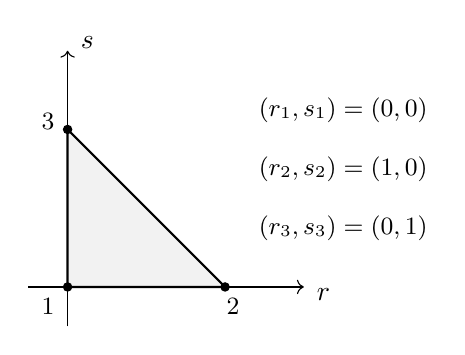
\begin{tikzpicture}
\draw[fill=gray!10,gray!10] (0.5,0.5)--(2.5,0.5)--(0.5,2.5)--cycle;
\draw[thick] (0.5,0.5)--(2.5,0.5)--(0.5,2.5)--cycle;
\draw [->] (0,0.5) -- (3.5,0.5);
\draw [->] (0.5,0) -- (0.5,3.5);
\node[] at (3.75,0.4) {$r$};
\node[] at (0.75,3.6) {$s$};
\draw[black,fill=black] (0.5,0.5)   circle (1.5pt);
\draw[black,fill=black] (2.5,0.5)   circle (1.5pt);
\draw[black,fill=black] (0.5,2.5)   circle (1.5pt);
\node[] at (0.25,0.25) {\small $1$};
\node[] at (2.6,0.25) {\small $2$};
\node[] at (0.25,2.6) {\small $3$};
\node[] at (4,2.75) {\small $(r_1,s_1)=(0,0)$};
\node[] at (4,2) {\small $(r_2,s_2)=(1,0)$};
\node[] at (4,1.25) {\small $(r_3,s_3)=(0,1)$};
\end{tikzpicture}
\end{center}
and the basis functions are simply
\begin{eqnarray}
\bN_1(r,s) &=& 1-r-s \\
\bN_2(r,s) &=& r \\
\bN_3(r,s) &=& s 
\end{eqnarray}
with the interpolation requirement $\bN_i(r_j,s_j)=\delta_{ij}$ fulfilled, 
as well as $\sum_i \bN_i=1$. 

Now, following the figure by Gresho and Sani, I build the reference element for the $P_1+P_0$ space:
\begin{center}
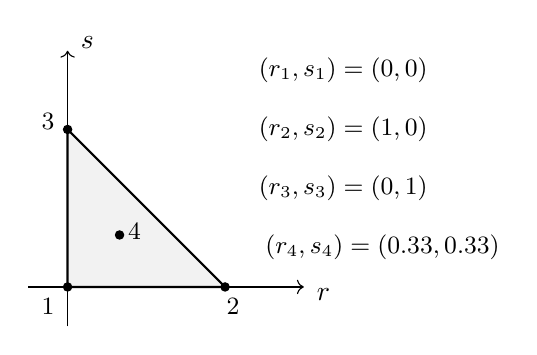
\begin{tikzpicture}
\draw[fill=gray!10,gray!10] (0.5,0.5)--(2.5,0.5)--(0.5,2.5)--cycle;
\draw[thick] (0.5,0.5)--(2.5,0.5)--(0.5,2.5)--cycle;
\draw [->] (0,0.5) -- (3.5,0.5);
\draw [->] (0.5,0) -- (0.5,3.5);
\node[] at (3.75,0.4) {$r$};
\node[] at (0.75,3.6) {$s$};
\draw[black,fill=black] (0.5,0.5)   circle (1.5pt);
\draw[black,fill=black] (2.5,0.5)   circle (1.5pt);
\draw[black,fill=black] (0.5,2.5)   circle (1.5pt);
\draw[black,fill=black] (1.16,1.16) circle (1.5pt);
\node[] at (0.25,0.25) {\small $1$};
\node[] at (2.6,0.25) {\small $2$};
\node[] at (0.25,2.6) {\small $3$};
\node[] at (1.35,1.2) {\small $4$};
\node[] at (4,3.25) {\small $(r_1,s_1)=(0,0)$};
\node[] at (4,2.5)    {\small $(r_2,s_2)=(1,0)$};
\node[] at (4,1.75) {\small $(r_3,s_3)=(0,1)$};
\node[] at (4.5,1) {\small $(r_4,s_4)=(0.33,0.33)$};
\end{tikzpicture}
\end{center}

$P_1+P_0$ means that the pressure inside the element is given by
\[
p^h(r,s) = a \bN_1(r,s)+ b\bN_2(r,s) + c\bN_3(r,s) + d\bN_4(r,s) 
\]
Note that it is then impossible to find $a,b,c,d$ such that the interpolation 
requirement $\bN_i(r_j,s_j)=\delta_{ij}$ is fulfilled.
In other words, the element is not interpolatory, i.e., there is no $\delta_{ij}$ property.% W.B. email

With regards to the 'element mass balance', W.B. states : 
\begin{displayquote}
{\color{darkgray}
the mass conservation requires that the function that is constant 1 
on one cell and zero on all other cells is part of the function space. 
That is indeed true -- it's the $\bN_4$ function. Indeed, that's the purpose of 
the enrichment with the $P_0$ part. It is not necessary that {\it all} shape functions are discontinuous.
}
\end{displayquote}




\textcite{bocg12} (2012) state: 
\begin{displayquote}
{\color{darkgray}
[...] the pressure space $Q_h$ is defined as the sum of two finite 
element spaces, namely $P_k+P_0$ ($k \ge d- 1$) [...] for the enhanced 
Hood–Taylor [...]. However, it can be easily observed that the sum is not direct, 
since globally constant functions can be represented exactly by means of piecewise 
$P_0$ or continuous $P_k$ ($k \ge 1$) elements.
Concerning the implementation of the method, we avoid the computation of the basis
functions of such a finite element by testing the discrete problem (2.3) 
with the basis 
functions of the two subspaces separately. By the above discussion it 
turns out that the resulting
matrix is rank-deficient, with kernel of dimension 1.
}
\end{displayquote}

The element pair is also discussed in \textcite{chen14} (2014).



%------------------------------------------------------------------
\subsubsection{The ${ Q}_2\times (Q_1+Q_0)$ pair} \label{ss:q2q1q0}
\begin{flushright} {\tiny {\color{gray} \tt  pair\_q2q1q0.tex}} \end{flushright}
%~~~~~~~~~~~~~~~~~~~~~~~~~~~~~~~~~~~~~~~~~~~~~~~~~~~~~~~~~~~~~~~~~~~~~~~~~~~~~~~~~~~~~~~~~~~~~~~~~~

It is a rather peculiar element pair (triplet?). The velocity space is the standard $Q_2$ space
but the pressure space is the sum of two spaces, i.e. $Q_1$ {\it and} $Q_0$.
Please see Section~\ref{ss:p2p1p0} on the ${\bm P}_2\times (P_1+P_0)$ element.

\begin{center}
\includegraphics[width=9cm]{images/pair_q2q1q0}\\
{\captionfont Taken from \textcite{grsa}'s book.}
\end{center}

It is implemented in \stone~120.


%------------------------------------------------------------------
\subsubsection{The ${ P}_3\times P_2$ pair} \label{ss:p3p2}
\index{general}{$P_3\times P_2 element$}
\begin{flushright} {\tiny {\color{gray} \tt pair\_p3p2.tex}} \end{flushright}
%~~~~~~~~~~~~~~~~~~~~~~~~~~~~~~~~~~~~~~~~~~~~~~~~~~~~~~~~~~~~~~~~~~~~~~~~~~~~~~~~~~~~~~~~~~~~~~~~~~

${\bm P}_3\times P_2$ mentioned in \textcite{sten90}.
The $P_3$ basis functions are presented in Section~\ref{basis:p3} and the $P_2$ basis
functions in Section~\ref{basis:p2}.
See \stone~120.


%------------------------------------------------------------------
\subsubsection{The Raviart-Thomas family} \label{ss:raviart_thomas}
\begin{flushright} {\tiny {\color{gray} \tt pair\_raviart\_thomas.tex}} \end{flushright}
%~~~~~~~~~~~~~~~~~~~~~~~~~~~~~~~~~~~~~~~~~~~~~~~~~~~~~~~~~~~~~~~~~~~~~~~~~~~~~~~~~~~~~~~~~~~~~~~~~~

- Raviart Thomas 0 RT0 \cite{rath77} ? mentioned/defined/drawn in 4.2.2 of 
Kanschat book. Also exist for quads see 4.2.37 
\textcite{hald03}: ``$P_1^\perp \times P_0$ symbol denotes an element with 
normal velocity nodes in the middle of each edge of the
triangulation [...]. This element, also called low order Raviart–Thomas element 
(Raviart and Thomas, 1977), is based on flux conservation on elements edges and 
the resulting scheme is very close to a finite volume scheme.''

Mentioned in \textcite{john16}, appendix B.3, example B.45: ``the normal component of v 
on each face is a constant. The normal component of functions from RT0 is
continuous across faces of the mesh cells.''

Check \textcite{brfo}

Mentioned in \textcite{chen93a} (1993).

\url{https://defelement.com/elements/raviart-thomas.html}


\url{
https://en.wikipedia.org/wiki/Raviart-Thomas_basis_functions
}

\url{
https://people.tamu.edu/~guermond//M661_FALL_2015/chap7.pdf
}

\url{
https://scicomp.stackexchange.com/questions/20245/raviart-thomas-elements-on-reference-square
}





%------------------------------------------------------------------
\subsubsection{The Bernaudi-Raugel pair} \label{ss:bernaudi_raugel}
\begin{flushright} {\tiny {\color{gray} pair\_bernaudi\_raugel.tex}} \end{flushright}
%~~~~~~~~~~~~~~~~~~~~~~~~~~~~~~~~~~~~~~~~~~~~~~~~~~~~~~~~~~~~~~~~~~~~~~~~~~~~~~~~~~~~~~~~~~~~~~~~~~

In \textcite{cakp15} (2015) we find: ``The BR-FEM after Bernardi and Raugel \cite{bera85} 
is a modification of the $P_2\times P_0$ FEM. It is sometimes also called reduced $P_2\times P_0$ FEM''.
They also state that this element also exists in 3D.

\begin{center}
\includegraphics[width=5cm]{images/pair_bernardi_raugel/cakp15}
\end{center}

It is also mentioned in \textcite{bobf13} although it seems it is there called the SMALL element (p474).

In Lederer: "Consider the case d = 2. [...] we only need to control 
the normal velocity at the edge, i.e. adding the
edge bubble for both components of the velocity seems to be sub optimal (with respect to
computational costs and the expected approximation properties). The idea now is to only
add the normal edge bubble."

According to \textcite{jolm17} (2017) (example 6.3), `` the velocity space in the Bernardi-Raugel
element consists of $P_1$ functions which are enriched with edge bubble functions''.
The authors also speak of 'reconstructing the test functions' and state: 
``the results of the method with reconstruction are generally more accurate.
In summary, the use of an appropriately reconstructed test function in the Bernardi–
Raugel pair of spaces led to a clear improvement of the accuracy of the computed
results compared with the standard method.''




%------------------------------------------------------------------
\subsubsection{The Scott-Vogelius pair} \label{ss:scott_vogelius}
\index{general}{Scott-Vogelius pair}
\begin{flushright} {\tiny {\color{gray} \tt pair\_scott\_vogelius.tex}} \end{flushright}
%~~~~~~~~~~~~~~~~~~~~~~~~~~~~~~~~~~~~~~~~~~~~~~~~~~~~~~~~~~~~~~~~~~~~~~~~~~~~~~~~~~~~~~~~~~~~~~~~~~

It originates in \fullcite{scvo85} (1985). 

 
In Remark 9 (p.29) of \textcite{aubb17} (2017) we find: 
\begin{displayquote}
{\color{darkgray}
We also remark that the discontinuous
pressure version of the Hood–Taylor element typically
results in an unstable method. However, stability can be
recovered by imposing certain restrictions on the mesh for
$k \ge 3$ (see \cite{voge83}; \cite{scvo85}), or
by taking advantage of suitable stabilization procedures for
$k\ge 1$ (see Mansfield, 1982; Boffi, 1995).
}
\end{displayquote}

In \textcite{fams21} (2021) we find:
\begin{displayquote}
{\color{darkgray}
The Scott-Vogelius element is given by choosing continuous piecewise 
polynomials of degree $k$ for the velocity and discontinuous piecewise 
polynomials of degree $k-1$ for the pressure. While this clearly
implies that $\nabla\cdot V_h \in Q_h$, inf-sup stability of the 
Scott–Vogelius element is more delicate, and is a topic of ongoing research. 
In two dimensions, Scott \& Vogelius proved \cite{scvo85} that the element is inf-sup
stable for $k\ge 4$ if the mesh does not have nearly singular vertices. 
In three dimensions, it was proven more recently in \cite{zhan11b} 
that the element is stable for $k\ge 6$ on uniform meshes. The stability on general
tetrahedral meshes continues to be an open question.

On barycentrically refined meshes, however, the pair is known to 
be stable for polynomial order
$k = d$, see [48, Section 4.6] for the 2D case and 
\cite{zhan05} for the 3D case. If one is willing to 
consider the more complicated Powell–Sabin split, the order 
can be reduced further to $k=d-1$ \cite{zhan08,zhan11a}. The two
refinement patterns are shown for the two dimensional case 
in Figure 1 [see below]. In this work we will consider
the case of $k \ge d$ on barycentrically refined meshes, but 
the arguments apply mutatis mutandis to the Powell–Sabin split.
}
\end{displayquote}

\begin{center}
\includegraphics[width=9cm]{images/pair_scott_vogelius/scottvogelius_split}\\
{\captionfont 
Barycentrically refined triangle (also known as Alfeld split) on the left,
and Powell–Sabin split on the right.\\ Taken from \textcite{fams21} (2021).}
\end{center}

\index{general}{Powell-Sabin}

\textcite{cael11} (2011) state:
\begin{displayquote}
{\color{darkgray}
The SV element pair is not yet very well known,
and so we now give a brief description of it. In essence, the SV pair is the same as
the Taylor-Hood pair except that the pressure space is discontinuous and either
(i) for $k \ge d$, the mesh is a barycenter refinement of a regular mesh, or
(ii) for $k = 2, d = 3$, the mesh is formed from a barycenter refined mesh by
connecting the barycenter nodes (i.e., a Powell–Sabin tetrahedralization).
In short, polynomials of degree $k$ and $k-1$ are used to approximate the velocity
and pressure spaces, respectively, and the mesh ${\cal T}_h$ that is used must be derived from
a regular triangulation (tetrahedralization) of $\Omega$, where each element is refined as
stated above. With these mesh constructions, it was proved by Zhang in [42, 44] that
the SV elements are LBB stable, and, consequently, also have optimal approximation
properties. It is well known that the TH pair is LBB stable and admits optimal
approximation properties for these cases as well [9]. We will restrict our definition of
SV elements to these cases where they are LBB stable.
}
\end{displayquote}

On page 112 of \textcite{john16} we read:
\begin{displayquote}
{\color{darkgray}
The Scott–Vogelius finite element considers still $P_k/P^{disc}_{k-1}$, $k \ge d$, 
but on special meshes, which allow to show the satisfaction of the 
discrete inf-sup condition.
[...]
This pair of finite element spaces $P_k/P^{disc}_{k-1}$
are weakly divergence-free, which is a desirable property.
[...]
The fulfillment of the discrete inf-sup condition 
was proved already in \textcite{scvo85} (1985) in the two-dimensional 
case for $k\ge 4$ if there is no so-called singular vertex in the mesh.
An internal vertex is said to be singular if edges which meet at the vertex fall onto
two straight lines.

The basic idea to overcome this problem consists in using meshes 
without singular vertices. To this end, so-called barycentric-refined 
grids are constructed. Starting from any admissible triangular mesh, 
new edges are introduced by connecting all
vertices of a mesh cell with the barycenter of this mesh cell. 
This step creates smaller triangles.
On barycentric-refined meshes, the $P_k/P^{disc}_{k-1}$, $k=2,3$ 
pair of finite element spaces was shown to satisfy the discrete inf-sup
condition in Qin's phd thesis (1994). [...]

The use of the $P_2/P^{disc}_{1}$ pair of finite element spaces 
on barycentric-refined meshes can be found occasionally in the literature,
in particular to demonstrate the advantages of using pairs of finite element 
spaces which provide weakly divergence-free velocity solutions, 
e.g. see \textcite{john15} and refs therein.

}
\end{displayquote}


\begin{center}
\includegraphics[width=6cm]{images/pair_scott_vogelius/john16}\\
{\captionfont Barycentric-refined simplicial grid on the unit square}
\end{center}

I hereafter present my own internal numbering for the mesh above (used in \stone~120 for example).
The quadrilateral has been cut once along a diagonal, and then an Alfeld split is used, thereby 
dividing the square in 6 triangles:

\input{tikz/tikz_sv.tex}

See also \textcite{jolm17} (2017) in which the $P_2\times P_1$, Scott-Vogelius ($P_2\times P_{-1}$), 
Bernardi-Raugel, and $P_2^+\times P_{-1}$ elements 
are compared for a thermo-mechanically driven convection problem in a triangle (see \stone~51, 
although I use the $P_1^+\times P_1$ element in this stone).


\begin{center}
\includegraphics[width=10cm]{images/pair_scott_vogelius/john_scott_vogelius}\\
\captionfont{Taken from John \cite[p70]{john16}.} 
\end{center}


In \textcite{befh21} (2021) this element is used in its 
$(P_3)^2-P_2^{\text{disc}}$ form.

Note that some have proposed to use an incenter-based refinement instead of
a barycenter refinement since it lead to less pronounced aspect ratios\footnote{
The Scott-Vogelius Method for Stokes Problem on Anisotropic Meshes, K Kean, M Neilan, M Schneier,
\url{https://doi.org/10.48550/arXiv.2109.14780}}.
In geometry, the incenter of a triangle is a triangle center, a point defined for 
any triangle in a way that is independent of the triangle's placement or scale. 
The incenter may be equivalently defined as the point where the internal angle bisectors 
of the triangle cross or as the point equidistant from the triangle's sides.

Given the coordinates of the three vertices of a triangle ABC,
the coordinates of the incenter O are
\[
x_O=\frac{ax_A+bx_B+cx_C}{a+b+c}
\qquad
y_O=\frac{ay_A+by_B+cy_C}{a+b+c}
\] 
where $a$, $b$ and $c$ are the side lengths opposite vertex A, B and C.

 
Note that \textcite{zhan24} (2024) proposes a solution to the unstable issue: 
\begin{displayquote}
{\color{darkgray}
We show that the discrete velocity solution converges at
the optimal order when solving the steady state Stokes
equations by the ${\bm P}_k\times P_{-(k-1)}$ mixed finite element method for
$k \ge 4$ on 2D triangular grids or $k \ge 6$ on tetrahedral grids,
even in the case the inf-sup condition fails. By a simple
$L_2$-projection of the discrete $P_{k-1}$ pressure to the space of
continuous $P_{k-1}$ polynomials, we show this post-processed
pressure solution also converges at the optimal order. Both
2D and 3D numerical tests are presented, verifying the
theory.
}
\end{displayquote}

Rather interestingly, we find in \textcite{tesk12} (2012) a penalty-approach:
\begin{displayquote}
{\color{darkgray}
Other solutions to deal with the LBB condition include the Uzawa iteration method and penalty
methods. A combination of these two approaches results in the iterated penalty method presented in
Scott and Vogelius (1985). Let $r\in\R$ and $\rho\in\R^+$ be prescribed parameters. 
We wish to find $u^n\in V_h$ such that 
\[
a(u^n,v) + r(\nabla\cdot u^n,\nabla\cdot v) = (f,v) - (\nabla \cdot v, \nabla\cdot w^n)
\qquad \forall \; v\in V_h,
\]
where $w^{n+1}=w^n+\rho u^n$.
The pressure may be recovered from the auxiliary field $w$ via $p=\nabla\cdot w -C$, 
where $C$ is an arbitrary constant (since the pressure field is only determined up 
to an arbitrary constant). When computing the error in $p$, we subtract the average 
of $\nabla\cdot w$ to account for $C$. The algorithm initially assumes
$w^0=0$, and then solves [the equation above] and updates $w$. 
The process is repeated until $\| u^{n+1}-u^n\|<\epsilon$, 
where $\epsilon$ is a prescribed tolerance. This method involves only one function space, but
it requires a higher-order continuous element $(q\ge 4)$ and it solves the divergence-free criterion
exactly. The iteration count and accuracy are dependent upon the penalty parameters $\rho$ and $r$. 
The implementation of this formulation is presented in [the following figure]:
\begin{center}
\includegraphics[width=6cm]{images/pair_scott_vogelius/tesk12}
\end{center}

}
\end{displayquote}



\begin{center}
\url{https://defelement.com/elements/scott-vogelius.html}
\end{center}




%------------------------------------------------------------------
\subsubsection{The BDM (Brezzi-Douglas-Marini) pair} \label{ss:bdm}
\index{general}{BDM element}
\index{general}{BDM element}
\begin{flushright} {\tiny {\color{gray} \tt  pair\_bdm.tex}} \end{flushright}
%~~~~~~~~~~~~~~~~~~~~~~~~~~~~~~~~~~~~~~~~~~~~~~~~~~~~~~~~~~~~~~~~~~~~~~~~~~~~~~~~~~~~~~~~~~~~~~~~~~

This element is mentioned in Kanschat book \cite{kanschat}, section 4.2.14. 
It also exists for quads see section 4.2.39 in the same book.
It is mentioned in \textcite{chen93a} (1993), also check the book by \textcite{brfo}.
It is well described in \textcite{kanschat17}.
There is an entire chapter (14) of \textcite{ergu21_72} dedicated to H(div) and 
section 14.5.1 to BDM elements. 
Check section 4.1.1 of \cite{aubb17} for triangles and quads.

\begin{center}
\url{https://defelement.com/elements/brezzi-douglas-marini.html}
\end{center}

\begin{itemize}
%++++++++++++++++++++++++++++++++++++++++++++++
\item In \textcite{lomw12} we read:

The Brezzi-Douglas-Marini element was introduced by Brezzi, Douglas and Marini in two dimensions 
(for triangles) in \textcite{brdm85} (1985). The element can be viewed as an alternative to the
Raviart-Thomas element using a complete polynomial space. It was later extended to three 
dimensions (tetrahedra, prisms and cubes) in \textcite{nede86} (1986) 
and \textcite{brdd87} (1987). The definition given
here is based on that of \textcite{nede86} (1986).

The Brezzi-Douglas-Marini element was introduced for mixed formulations of second-order elliptic 
equations. However, it is also useful for weakly symmetric discretizations of the elastic stress
tensor; see Farhloul and Fortin (1997); Arnold et al. (2007).

\begin{center}
\includegraphics[width=8cm]{images/pair_bdm/bdm_lomw12}\\
{\captionfont Taken from \cite{lomw12}. }
\end{center}

The dimension of $BDM_q$ is $(q+1)(q+2)$ for a triangle and $\frac12(q+1)(q+2)(q+3)$
for a tetrahedron.

Check book for definition.

A slight modification of the Brezzi-Douglas-Marini element constrains the element space ${\cal V}$ by
only allowing normal components on the boundary of polynomial degree $q-1$ (rather than the full
polynomial degree $q$). Such an element was suggested on rectangles by \textcite{brdf87} (1987), and the
triangular analogue was given in \textcite{brfo}. In similar spirit, elements with differing
degrees on the boundary suitable for varying the polynomial degree between triangles were derived
in \textcite{brdm85b} (1985).

%++++++++++++++++++++++++++++++++++++++++++++++
\item On the defelement website\footnote{\url{https://defelement.org/elements/brezzi-douglas-marini.html}}
we find a lot of information. Note that the mapping is set to 'contravariant Piola'. 
\todo[inline]{I still need to understand and write about this!}
It belongs to the categories 'Vector-valued elements', and 'H(div) conforming elements'

\begin{center}
\input{images/pair_bdm/ref-triangle.tex}\\
{\captionfont Taken from DefElement \url{https://defelement.org/img/ref-triangle.html}. I have altered 
the font size. Orange: nodes; Blue: edges.}
\end{center}


I reproduce below the figures and basis functions pertaining to the Degree 1 triangle, 
but the site also shows Degree 2 triangle, Degree 1 \& 2 tetrahedron, and so-called 
Lagrange variants.

\begin{center}
\includegraphics[width=3cm]{images/pair_bdm/element-Brezzi-Douglas-Marini-variant-equispaced-triangle-1-dofs}
\includegraphics[width=3cm]{images/pair_bdm/element-Brezzi-Douglas-Marini-variant-equispaced-triangle-1-0}
\includegraphics[width=3cm]{images/pair_bdm/element-Brezzi-Douglas-Marini-variant-equispaced-triangle-1-1}
\includegraphics[width=3cm]{images/pair_bdm/element-Brezzi-Douglas-Marini-variant-equispaced-triangle-1-2}\\
\includegraphics[width=3cm]{images/pair_bdm/element-Brezzi-Douglas-Marini-variant-equispaced-triangle-1-3}
\includegraphics[width=3cm]{images/pair_bdm/element-Brezzi-Douglas-Marini-variant-equispaced-triangle-1-4}
\includegraphics[width=3cm]{images/pair_bdm/element-Brezzi-Douglas-Marini-variant-equispaced-triangle-1-5}\\
{\captionfont Pink: degrees of freedom.}
\end{center}


${\cal V}$ is spanned by 
\[
\left(\begin{array}{c}
1 \\ 0
\end{array}\right),
\left(\begin{array}{c}
0 \\ 1
\end{array}\right),
\left(\begin{array}{c}
x \\ 0
\end{array}\right),
\left(\begin{array}{c}
0 \\ x
\end{array}\right),
\left(\begin{array}{c}
y \\ 0
\end{array}\right),
\left(\begin{array}{c}
0 \\ y
\end{array}\right)
\]
with 
\begin{itemize}
\item DOF \#0 is associated with edge 0 of the reference element with $\vec{\bN}_0$ basis function.
\item DOF \#1 is associated with edge 0 of the reference element with $\vec{\bN}_1$ basis function.
\item DOF \#2 is associated with edge 1 of the reference element with $\vec{\bN}_2$ basis function.
\item DOF \#3 is associated with edge 1 of the reference element with $\vec{\bN}_3$ basis function.
\item DOF \#4 is associated with edge 2 of the reference element with $\vec{\bN}_4$ basis function.
\item DOF \#5 is associated with edge 2 of the reference element with $\vec{\bN}_5$ basis function.
\end{itemize}
and
\begin{eqnarray}
\vec{\bN}_0 &=&  \left(\begin{array}{c} -4x \\ 2y        \end{array}\right) \nn\\  
\vec{\bN}_1 &=&  \left(\begin{array}{c} 2x \\ -4y        \end{array}\right) \nn\\  
\vec{\bN}_2 &=&  \left(\begin{array}{c} 4x+6y-4 \\ -2y   \end{array}\right) \nn\\  
\vec{\bN}_3 &=&  \left(\begin{array}{c} -2x-6y+2 \\ 4y   \end{array}\right) \nn\\  
\vec{\bN}_4 &=&  \left(\begin{array}{c} 2x \\ -6x-4y+4   \end{array}\right) \nn\\  
\vec{\bN}_5 &=&  \left(\begin{array}{c} -4x \\ 6x +2y -2 \end{array}\right) \nn
\end{eqnarray}

 

\item In \cite{brdf87} we read:
\begin{displayquote}
The object of this paper is to present families of rectangular mixed finite
éléments that are derived from the elements of \cite{brdm85} 
in two space variables and of \cite{brdd87} in three space variables.
\end{displayquote}














\end{itemize}



%------------------------------------------------------------------
\subsubsection{The DSSY pair} \label{ss:pair_dssy2D}
\index{general}{Nonconforming element}
\index{general}{DSSY element}
\index{general}{Nonconforming element}
\index{general}{DSSY element}
\begin{flushright} {\tiny {\color{gray} \tt pair\_dssy2D.tex}} \end{flushright}
%~~~~~~~~~~~~~~~~~~~~~~~~~~~~~~~~~~~~~~~~~~~~~~~~~~~~~~~~~~~~~~~~~~~~~~~~~~~~~~~~~~~~~~~~~~~~~~~~~~

This element is often referred to as the 'DSSY' element because of the 
four authors of the original paper: Douglas, Santos, sheen and Ye (1999) \cite{doss99}.

The non-conforming finite element space $Q_l$ is defined based on the 
reference square element on $[-1,1]^2$ :
\[
Q_l = \text{Span} \left\{ 1, r, s, \theta_l(r)-\theta_l(s)  \right\}
\qquad l=1,\; \text{or} \; 2
\]
with
\begin{eqnarray}
\theta_1(r)  &=& r^2-\frac53r^4  \nn\\
\theta_1'(r) &=& 2r-\frac{20}{3}r^3  \nn\\
\theta_2(r)  &=& r^2-\frac{25}{6} r^4 + \frac72 r^6 \\ 
\theta_2'(r) &=& 2r-\frac{50}{3} r^3 + 21 r^5
\end{eqnarray}
The dimension of $Q_l$ is four and the $\theta_l$ functions look like:
\begin{center}
\includegraphics[width=7cm]{images/dssy/theta1}
\includegraphics[width=7cm]{images/dssy/theta2}
\end{center}
We have:
\begin{itemize}
\item $\theta_1(r=-1)=\theta_1(r=+1)=-\frac23$, $\theta_1(r=0)=0$ 
\item $\theta_2(r=-1)=\theta_2(r=+1)=\frac13$, $\theta_2(r=0)=0$ 
\end{itemize}
The nodes are situated at the mid-edges of the quadrilateral:

\input{tikz/tikz_dssy2D}

The basis function corresponding to the node (1, 0) is given by
\begin{mdframed}[backgroundcolor=blue!5]
\begin{eqnarray}
\bN_1(r,s)^{(l)} &=& \frac{1}{4} - \frac{1}{2} r + \frac{\theta_l(r)-\theta_l(s)}{4 \theta_l(1)}  \nn\\
\bN_2(r,s)^{(l)} &=& \frac{1}{4} + \frac{1}{2} r + \frac{\theta_l(r)-\theta_l(s)}{4 \theta_l(1)}  \nn\\
\bN_3(r,s)^{(l)} &=& \frac{1}{4} - \frac{1}{2} s - \frac{\theta_l(r)-\theta_l(s)}{4 \theta_l(1)}  \nn\\
\bN_4(r,s)^{(l)} &=& \frac{1}{4} + \frac{1}{2} s - \frac{\theta_l(r)-\theta_l(s)}{4 \theta_l(1)}  
\end{eqnarray}
\end{mdframed}
We can easily verify that $\sum\limits_i \bN_i(r,s,t)=1$ and that $\bN_i(\vec{r}_j)=\delta_{ij}$:
\begin{eqnarray}
\bN_1^{(l)}(r_1,s_1) 
&=& \frac{1}{4} -\frac{1}{2} (-1) + \frac{\theta_l(-1)-\theta_l(0)}{4 \theta_l(1)}  
= \frac{1}{4} +\frac{1}{2}  + \frac{\theta_l(-1)}{4 \theta_l(1)}  
= \frac{1}{4} +\frac{1}{2}  + \frac{1}{4}   = 1 \nn\\
\bN_1^{(l)}(r_2,s_2)
&=& \frac{1}{4} -\frac{1}{2} (+1) + \frac{\theta_l(+1)-\theta_l(0)}{4 \theta_l(1)}  
= \frac{1}{4} -\frac{1}{2} + \frac{\theta_l(+1)}{4 \theta_l(1)}  
= \frac{1}{4} -\frac{1}{2} + \frac{1}{4}   = 0 \nn\\
\bN_1^{(l)}(r_3,s_3)
&=& \frac{1}{4} -\frac{1}{2} (0) + \frac{\theta_l(0)-\theta_l(-1)}{4 \theta_l(1)}  
= \frac14 -\frac14  = 0 \nn\\
\bN_1^{(l)}(r_4,s_4)
&=& \frac{1}{4} -\frac{1}{2} (0) + \frac{\theta_l(0)-\theta_l(+1)}{4 \theta_l(1)}  
= \frac14 -\frac14  = 0 \nn\\
\bN_2^{(l)}(r_1,s_1) 
&=& \frac{1}{4} + \frac{1}{2} (-1) + \frac{\theta_l(-1)-\theta_l(0)}{4 \theta_l(1)}  
= \frac14 -\frac12 + \frac14 = 0 \nn\\
\bN_2^{(l)}(r_2,s_2)
&=& \frac{1}{4} + \frac{1}{2} (+1) + \frac{\theta_l(+1)-\theta_l(0)}{4 \theta_l(1)}  
= \frac14 + \frac12 + \frac14 =1 \nn\\
\bN_2^{(l)}(r_3,s_3)
&=& \frac{1}{4} + \frac{1}{2} (0) + \frac{\theta_l(0)-\theta_l(-1)}{4 \theta_l(1)}  
= \frac14 - \frac14 = 0 \nn\\
\bN_2^{(l)}(r_4,s_4)
&=& \frac{1}{4} + \frac{1}{2} (0) + \frac{\theta_l(0)-\theta_l(+1)}{4 \theta_l(1)}  
= \frac14 - \frac14 = 0 \nn\\
\bN_3^{(l)}(r_1,s_1)
&=& \frac{1}{4} - \frac{1}{2} (0) - \frac{\theta_l(-1)-\theta_l(0)}{4 \theta_l(1)} 
= \frac14 -\frac14 = 0\nn\\
\bN_3^{(l)}(r_2,s_2)
&=& \frac{1}{4} - \frac{1}{2} (0) - \frac{\theta_l(+1)-\theta_l(0)}{4 \theta_l(1)} 
= \frac14 -\frac14 = 0\nn\\
\bN_3^{(l)}(r_3,s_3)
&=& \frac{1}{4} - \frac{1}{2} (-1) - \frac{\theta_l(0)-\theta_l(-1)}{4 \theta_l(1)} 
= \frac14 +\frac12 + \frac14 = 1\nn\\
\bN_3^{(l)}(r_4,s_4)
&=& \frac{1}{4} - \frac{1}{2} (+1) - \frac{\theta_l(0)-\theta_l(+1)}{4 \theta_l(1)} 
= \frac14 -\frac12 + \frac14 = 0\nn\\
\bN_4^{(l)}(r_1,s_1)
&=& \frac{1}{4} + \frac{1}{2} (0) - \frac{\theta_l(-1)-\theta_l(0)}{4 \theta_l(1)}  
= \frac14 -\frac14 =0\nn\\
\bN_4^{(l)}(r_2,s_2)
&=& \frac{1}{4} + \frac{1}{2} (0) - \frac{\theta_l(+1)-\theta_l(0)}{4 \theta_l(1)}  
= \frac14 -\frac14 =0\nn\\
\bN_4^{(l)}(r_3,s_3)
&=& \frac{1}{4} + \frac{1}{2} (-1) - \frac{\theta_l(0)-\theta_l(-1)}{4 \theta_l(1)}  
= \frac14 -\frac12 +\frac14 = 0 \nn\\
\bN_4^{(l)}(r_4,s_4)
&=& \frac{1}{4} + \frac{1}{2} (1) - \frac{\theta_l(0)-\theta_l(1)}{4 \theta_l(1)}  
= \frac14 +\frac12 +\frac14 = 1 \nn
\end{eqnarray}

The basis functions can also be explicitly written for $\theta_1$ as in Cai \etal \cite{cady99}:
\begin{eqnarray}
\bN_1(r,s)^{(l)} 
&=& \frac{1}{4} - \frac{1}{2} r - \frac38 \left[\left( r^2-\frac53r^4 \right) - \left(s^2-\frac53s^4 \right) \right] \nn\\
\bN_2(r,s)^{(l)} 
&=& \frac{1}{4} + \frac{1}{2} r - \frac38 \left[\left( r^2-\frac53r^4 \right) - \left(s^2-\frac53s^4 \right) \right] \nn\\
\bN_3(r,s)^{(l)} 
&=& \frac{1}{4} - \frac{1}{2} s + \frac38 \left[\left( r^2-\frac53r^4 \right) - \left(s^2-\frac53s^4 \right) \right] \nn\\
\bN_4(r,s)^{(l)} 
&=& \frac{1}{4} + \frac{1}{2} s + \frac38 \left[\left( r^2-\frac53r^4 \right) - \left(s^2-\frac53s^4 \right) \right] 
\end{eqnarray}

The derivatives of the basis functions are as follows:
\begin{eqnarray}
\partial_r \bN_1(r,s)^{(l)} &=&  - \frac{1}{2}  + \frac{\theta_l'(r)}{4 \theta_l(1)}  \nn\\
\partial_r \bN_2(r,s)^{(l)} &=&  + \frac{1}{2}  + \frac{\theta_l'(r)}{4 \theta_l(1)}  \nn\\
\partial_r \bN_3(r,s)^{(l)} &=&  - \frac{\theta_l'(r)}{4 \theta_l(1)}  \nn\\
\partial_r \bN_4(r,s)^{(l)} &=&  - \frac{\theta_l'(r)}{4 \theta_l(1)}  
\end{eqnarray}

\begin{eqnarray}
\partial_s \bN_1(r,s)^{(l)} &=&   -\frac{\theta_l'(s)}{4 \theta_l(1)}  \nn\\
\partial_s \bN_2(r,s)^{(l)} &=&   -\frac{\theta_l'(s)}{4 \theta_l(1)}  \nn\\
\partial_s \bN_3(r,s)^{(l)} &=&   - \frac{1}{2} + \frac{\theta_l'(s)}{4 \theta_l(1)}  \nn\\
\partial_s \bN_4(r,s)^{(l)} &=&   + \frac{1}{2} + \frac{\theta_l'(s)}{4 \theta_l(1)}  
\end{eqnarray}



Note that a correction was issued in \textcite{cads00} (2000) if a 
true quadrilateral (i.e., one having two opposite, nonparallel edges) is included in
the partition. The authors state that in the case of rectangles the original method is fine.

\Literature: 
Park \& Sheen (2003) \cite{pash03},
Jeon \etal (2013) \cite{jens13},
Park, Sheen \& Shin (2013) \cite{pass13},
Bangerth \etal (2017) \cite{baks17},
Sheen (2020) \cite{shee20}


%------------------------------------------------------------------
\subsubsection{The Han pair} \label{ss:han}
\index{general}{Han element}
\index{general}{Nonconforming element}
\index{general}{Han element}
\index{general}{Nonconforming element}
\begin{flushright} {\tiny {\color{gray} \tt  pair\_han.tex}} \end{flushright}
%~~~~~~~~~~~~~~~~~~~~~~~~~~~~~~~~~~~~~~~~~~~~~~~~~~~~~~~~~~~~~~~~~~~~~~~~~~~~~~~~~~~~~~~~~~~~~~~~~~

It is based on \textcite{han84} (also mentioned in Sheen (2020) \cite{shee20}).
The nodes are at the same location as for the RT element above, but 
there is an additional bubble function in the middle:

\input{tikz/tikz_han}

Inside the reference element we assume that a field $f$
can be represented by 
\begin{eqnarray}
f^h(r,s) 
%&=& a+ br +cs +d \phi(r) +e \phi(s) \nn\\
&=& a+ br +cs +d \underbrace{\frac{5r^4-3r^2}{2}}_{\phi(r)}
+e \underbrace{\frac{5s^4-3s^2}{2}}_{\phi(s)} \nn
\end{eqnarray}
We then must have 
\begin{align}
f_1 &= f^h(r=1,s=0) &= a+ b +d \nn\\
f_2 &= f^h(r=0,s=1) &= a+ c +e \nn\\
f_3 &= f^h(r=-1,s=0) &= a- b +d \nn\\
f_4 &= f^h(r=0,s=-1) &= a -c +e \nn\\
f_5 &= f^h(r=0,s=0) &= a  \nn
\end{align}
and we easily get 
\[
a = f_5 
\qquad
f_1-f_3 = 2b
\qquad 
f_2-f_4 = 2c
\]
followed by
\[
d=f_1-a-b = f_1 - f_5 - \frac{1}{2}(f_1-f_3) = \frac{f_1-2f_5+f_3}{2}
\]
and 
\[
e = f_2-a-c = f_2 - f_5 -  \frac{1}{2}(f_2-f_4) = \frac{f_2 -2f_5+f_4 }{2}
\]
Finally:
\[
f(r,s) = 
f_5 +
\frac{1}{2}(f_1-f_3) r+
\frac{1}{2}(f_2-f_4) s+
\frac{f_1-2f_5+f_3}{2} \phi(r)+
\frac{f_2 -2f_5+f_4 }{2} \phi(s)
\]
i.e.
\[
f(r,s) = 
\left(\frac{r + \phi(r)}{2} \right)f_1 +
\left(\frac{s+\phi(s)}{2} \right)f_2 +
\left(-\frac{r-\phi(r)}{2} \right)f_3 +
\left(-\frac{s - \phi(s)}{2} \right)f_4 +
\left(1-\phi(r)-\phi(s) \right)f_5 
\]
which has us define 
\begin{eqnarray}
\bN_1(r,s) &=& \frac{r + \phi(r)}{2} \nn\\
\bN_2(r,s) &=& \frac{s+\phi(s)}{2} \nn\\
\bN_3(r,s) &=& -\frac{r-\phi(r)}{2} \nn\\
\bN_4(r,s) &=& -\frac{s - \phi(s)}{2}\nn\\
\bN_5(r,s) &=& 1-\phi(r)-\phi(s)\nn
\end{eqnarray}
We have of course the following properties $\sum\limits_{i=1}^5 \bN_i(r,s) = 1$ and 
$\bN_i(r_j,s_j) = \delta_{ij},\;  i,j \in 1,5$. 
The partial derivatives of the basis functions are as follows
\begin{eqnarray}
\partial_r \bN_1(r,s) &=& \frac{1 + \phi'(r)}{2} \nn\\
\partial_r \bN_2(r,s) &=& 0 \nn\\
\partial_r \bN_3(r,s) &=& -\frac{1-\phi'(r)}{2} \nn\\
\partial_r \bN_4(r,s) &=& 0 \nn\\
\partial_r \bN_5(r,s) &=& -\phi'(r) \nn\\
\partial_s \bN_1(r,s) &=& 0 \nn\\
\partial_s \bN_2(r,s) &=& \frac{1 + \phi'(s)}{2} \nn\\
\partial_s \bN_3(r,s) &=&  0 \nn\\
\partial_s \bN_4(r,s) &=& -\frac{1-\phi'(s)}{2} \nn\\
\partial_s \bN_5(r,s) &=& -\phi'(s) \nn
\end{eqnarray}
This element is implemented in the {\tt stone\_han.py} file in \stone~77 and also in \stone~120. 








%------------------------------------------------------------------
\subsubsection{The Divergence-free nonconforming $P_1^{NC}\times P_0$ pair} \label{ss:p1ncp0}
\begin{flushright} {\tiny {\color{gray} \tt pair\_p1ncp0.tex}} \end{flushright}
%~~~~~~~~~~~~~~~~~~~~~~~~~~~~~~~~~~~~~~~~~~~~~~~~~~~~~~~~~~~~~~~~~~~~~~~~~~~~~~~~~~~~~~~~~~~~~~~~~~

It belongs to the Crouzeix-Raviart family. 
The midside nodes are used as degrees of freedom for the velocities.
It is mentioned in Section~6.3 of \textcite{bobf08} (2008): 
\begin{displayquote}
{\color{darkgray}
[...]
It is exactly divergence free. Another important feature of this
element is that it can be seen as a "mass conservation" scheme. The present element
has been generalized to second order in \textcite{foso83} (1983).
It must also be said that coerciveness may be a problem for the $P_1^{NC} \times P_0$ 
element, as it does not satisfy the discrete version of Korn's inequality. 
This issue has been deeply investigated and clearly illustrated in \textcite{arno93} (1993).}
\end{displayquote}

\input{tikz/tikz_p1ncp0}

At page 170 of \cite{braess} it is stated that {\color{darkgray} ``an analogous quadrilateral element was 
developed and studied by \textcite{ratu92} (1992)''} (see Section~\ref{ss:RTq1p0}).

In \textcite{bobf13} we find: 
\begin{displayquote}
{\color{darkgray}
We consider the classical (almost\footnote{What does that mean?!}) 
stable nonconforming triangular 
element introduced in \textcite{crra73}, in which mid-side nodes are used as degrees of 
freedom for the velocities. This generates
a piecewise linear nonconforming approximation; pressures are taken constant on
each element. It is also possible to build a three-dimensional
version of this element, using mid-face nodes as degrees of freedom.
\\
..
\\
It must also be recalled that coercivity is a problem for the $P_1^{NC}\times P_0$ 
element. The trouble is that the bilinear form (8.2.1) is not coercive on the 
nonconforming space $V_h$ and we do not have the discrete version of Korn's inequality.}
\end{displayquote}


It is also mentioned in \textcite{john16}, appendix B.3, example B.43, in 2D and 3D, 
in \textcite{brfo} (example 8.1), and studied extensively in \textcite{john98} (1998). 

\begin{center}
\includegraphics[width=8cm]{images/pair_p1ncp0/john98}\\
{\captionfont Taken from \textcite{john98}.}
\end{center}

In \textcite{jolm17} (2017) the authors show results obtained with this element (fig 6) 
but also explain that these are obtained with so-called reconstructed test functions.
 


%------------------------------------------------------------------
\subsubsection{The Chen nonconforming ${ Q}_1\times Q_0$ pair (?)} \label{ss:chenq0}
\begin{flushright} {\tiny {\color{gray} \tt pair\_chen.tex}} \end{flushright}
%~~~~~~~~~~~~~~~~~~~~~~~~~~~~~~~~~~~~~~~~~~~~~~~~~~~~~~~~~~~~~~~~~~~~~~~~~~~~~~~~~~~~~~~~~~~~~~~~~~

What follows is tentative!

This space is proposed in \textcite{chen93b} (1993), albeit not in the 
context of the Stokes equations.

It is based on the mid-point variant of the RT basis functions, 
\begin{eqnarray}
\bN_1(r,s) &=& \frac{1}{4} (1-2s-(r^2-s^2)) \nonumber\\
\bN_2(r,s) &=& \frac{1}{4} (1+2r+(r^2-s^2)) \nonumber\\
\bN_3(r,s) &=& \frac{1}{4} (1+2s-(r^2-s^2)) \nonumber\\
\bN_4(r,s) &=& \frac{1}{4} (1-2r+(r^2-s^2)) \nonumber
\end{eqnarray}
to which a $P_2$ bubble is added
\[
\phi(r,s) = 1-\frac34(r^2+s^2)
\]
Note thath this function is zero at locations $\pm 1/\sqrt{3}$ 
on all four edges and exactly 1 in the middle. 

A field $f$ is represented inside the element by 
\[
f^h(r,s)=a \bN_1(r,s)
+b \bN_2(r,s)
+c \bN_3(r,s)
+d \bN_4(r,s)
+e \phi(r,s)
\]
We immediately see that this space is not interpolatory, i.e. the basis function $\phi(r,s)$ cannot be 1 in the middle and 0 at the other four nodes. 

\textcite{chen} also extends this to 3D in the paper. 

This space is used for velocity and a $Q_0$ space is used for 
pressure in \stone~120 (only because the basis functions above are
based on the Rannacher-Turek ones).


%----------------------------
\subsubsection{Other FE element pairs}

\begin{itemize}

\item ${\bm Q}_2\times Q_2$: This element is never used, probably because 
a) it is unstable, b) it is very costly. 
There is one reference to it in \cite{hufb86}.

\item ${\bm Q}_1\times P_{-1}$ Bilinear velocities,  piecewise linear discontinuous polynomial pressure.

\item See Fortin \cite{fort81} for various stable low order elements other than the enriched 
${\bm Q}_1^+ \times P_0$

\item ${\bm Q}_1\times Q_1$ + nonconforming null edge average \cite{fros07}

\item check \textcite{dhhu86} (1986) many flavours of triangles and quads.

\item Bercovier-Pironneau element pair, or $P_1isoP_2$.See \textcite{bocg12} (2012).

\end{itemize}

%.........................................................................
\subsubsection{A note about incompressibility and standard mixed methods}

What follows is nicely explained and demonstrated in John \etal \cite{jolm17}. In their 
example 1.1 they look at the velocity error of benchmark VJ2 (see Section~\ref{mms9}) 
which analytical solution is a zero velocity field. They show that for the MINI, 
Taylor-Hood and Crouzeix-Raviart triangular elements the velocity error grows 
with the magnitude of the rhs. They also make this statement:
``there are important applications, e.g., natural
convection problems, where the pressure is larger than the velocity by orders
of magnitude. In such situations, one cannot expect to compute accurate
velocity fields with classical mixed methods, at least for low order methods.''


 %-----------------

\newpage
\section{The penalty approach for viscous flow}\label{sec:penalty}\input{penalty} %-------------
\newpage
\section{The mixed FEM for viscous flow} \label{sec:mixed} \index{general}{Mixed Formulation}
\begin{flushright} {\tiny {\color{gray} mixed.tex}} \end{flushright}

\subsection{In three dimensions}

The FEM formulation of the Stokes equation is quite complex so 
we simplify things as much as possible for now by 
assuming the flow to be \underline{incompressible}, 
\underline{isoviscous} and \underline{isothermal}. 

The methodology to derive the discretised equations of the mixed system is 
quite similar to the one we have used in the case of the penalty formulation.
The big difference comes from the fact that we are now solving for both 
velocity and pressure at the same time, and that we therefore must solve 
the mass and momentum conservation equations together.
As before, velocity inside an element is given by 
\begin{equation}
{\vec \upnu}^h({\vec r})=\sum_{i=1}^{m_v} \bN_i^\upnu({\vec r})\;  {\vec \upnu}_i
\label{mixed01}
\end{equation}
where $N_i^{\upnu}$ are the polynomial basis functions for the velocity,
and the summation runs over the $m_v$ velocity nodes composing the element.
A similar expression is used for pressure:
\begin{equation}
p^h({\vec r})=\sum_{i=1}^{m_p} \bN_i^p({\vec r}) \; p_i
\label{mixed02}
\end{equation}
Note that the velocity is a vector while pressure (and temperature)
is a scalar. There are then $ndof_v=ndim$ velocity degrees of freedom per node
and $ndof_p=1$ pressure degrees of freedom.
It is also very important to remember that the numbers of 
velocity nodes and pressure nodes for a given element 
are more often than not different and that velocity and pressure
nodes need not be colocated. Indeed, unless 
so-called 'stabilised elements' are used, we have $m_v>m_p$, which 
means that the polynomial order of the velocity field is higher than 
the polynomial order of the pressure field (usually by value 1).

Other notations will be sometimes used for Eqs.~\eqref{mixed01} and \eqref{mixed02}:
\begin{equation}
u^h({\vec r}) = \vec{\bN}^\upnu \cdot \vec{u}
\quad\quad\quad\quad
v^h({\vec r}) = \vec{\bN}^\upnu \cdot \vec{v}
\quad\quad\quad\quad
w^h({\vec r}) = \vec{\bN}^\upnu \cdot \vec{w}
\quad\quad\quad\quad
p^h({\vec r}) = \vec{\bN}^p \cdot \vec{p}
\end{equation} 
where ${\vec \upnu}=(u,v,w)$ and $\vec{\bN}^\upnu$ is the vector containing 
all basis functions evaluated at location ${\vec r}$:
\begin{eqnarray}
\vec{\bN}^v &=& \left( \bN_1^\upnu({\vec r}),  \bN_2^\upnu({\vec r}),  
\bN_3^\upnu({\vec r}), \dots  \bN_{m_v}^\upnu({\vec r}) \right) \\
\vec{\bN}^p &=& \left( \bN_1^p({\vec r}),  \bN_2^p({\vec r}),  
\bN_3^p({\vec r}), \dots  \bN_{m_p}^p({\vec r}) \right)
\end{eqnarray}
and with 
\begin{eqnarray}
\vec{u} &=& \left( u_1,  u_2,  u_3, \dots  u_{m_v} \right) \\
\vec{v} &=& \left( v_1,  v_2,  v_3, \dots  v_{m_v} \right) \\
\vec{w} &=& \left( w_1,  w_2,  w_3, \dots  w_{m_v} \right) \\
\vec{p} &=& \left( p_1,  p_2,  p_3, \dots  p_{m_p} \right) 
\end{eqnarray}
We will now establish the weak form of the momentum conservation equation. 
We start again from 
\begin{eqnarray}
{\vec \nabla}\cdot {\bm \sigma} + {\vec b} &=& {\vec 0} \\
{\vec \nabla}\cdot {\vec \upnu} &=& 0
\end{eqnarray}
For the $\bN_i^\upnu$'s and $\bN_i^p$ 'regular enough', we can write:
\begin{eqnarray}
\int_{\Omega_e} \bN_i^\upnu {\vec \nabla}\cdot {\bm \sigma}\;  dV
+ \int_{\Omega_e} \bN_i^\upnu  {\vec b} \; dV
&=& \vec 0 \\
\int_{\Omega_e} \bN_i^p {\vec \nabla}\cdot {\vec v} \; dV &=& 0
\end{eqnarray}
We can integrate by parts and drop the surface term\footnote{We will come back to this at a later stage}:
\begin{eqnarray}
\int_{\Omega_e} {\vec \nabla } \bN_i^\upnu \cdot {\bm \sigma} dV
&=& \int_{\Omega_e} \bN_i^\upnu  {\vec b} \; dV \\
\int_{\Omega_e} \bN_i^p {\vec \nabla}\cdot {\vec v} \; dV &=& 0
\end{eqnarray}
or, 
\begin{equation}
\int_{\Omega_e} 
\left(
\begin{array}{cccccc}
\frac{\partial \bN_i^\upnu}{\partial x} & 0 & 0& 
\frac{\partial \bN_i^\upnu}{\partial y} & 
\frac{\partial \bN_i^\upnu}{\partial z} & 0\\  \\
0 & \frac{\partial \bN_i^\upnu}{\partial y} & 0  & 
\frac{\partial \bN_i^\upnu}{\partial x}  & 0 &
\frac{\partial \bN_i^\upnu}{\partial z}  \\ \\
0 & 0 & \frac{\partial \bN_i^\upnu}{\partial z} &  0 & 
\frac{\partial \bN_i^\upnu}{\partial x} &  
\frac{\partial \bN_i^\upnu}{\partial y} 
\end{array}
\right)
\cdot
\left(
\begin{array}{c}
\sigma_{xx}\\
\sigma_{yy}\\
\sigma_{zz}\\
\sigma_{xy}\\
\sigma_{xz}\\
\sigma_{yz}\\
\end{array}
\right)
d\Omega = \int_{\Omega_e} \bN_i^\upnu {\vec b} \; dV
\end{equation}
The above equation can ultimately be written:
\begin{equation}
\int_{\Omega_e} {\bm B}^T \cdot 
\left(
\begin{array}{c}
\sigma_{xx}\\
\sigma_{yy}\\
\sigma_{zz}\\
\sigma_{xy}\\
\sigma_{xz}\\
\sigma_{yz}
\end{array}
\right)
dV
=
\int_{\Omega_e} {\vec \bN}_b\; dV
\end{equation}
We have previously established that the strain rate 
vector $\vec{\dot \varepsilon}$ is:
\begin{equation}
\vec{\dot\varepsilon}=
\left(
\begin{array}{c}
\frac{\partial u}{\partial x} \\ \\
\frac{\partial v}{\partial y} \\ \\
\frac{\partial w}{\partial z} \\ \\
\frac{\partial u}{\partial y}\! +\! \frac{\partial v}{\partial x} \\ \\
\frac{\partial u}{\partial z}\! +\! \frac{\partial w}{\partial x} \\ \\
\frac{\partial v}{\partial z}\! +\! \frac{\partial w}{\partial y} 
\end{array}
\right)
=
\left(
\begin{array}{c}
\sum\limits_i \frac{\partial \bN_i^\upnu}{\partial x} u_i \\ \\
\sum\limits_i \frac{\partial \bN_i^\upnu}{\partial y} v_i \\ \\
\sum\limits_i \frac{\partial \bN_i^\upnu}{\partial z} w_i \\ \\
\sum\limits_i (\frac{\partial \bN_i^\upnu}{\partial y} u_i\! +\! 
\frac{\partial \bN_i^\upnu}{\partial x} v_i) \\ \\
\sum\limits_i (\frac{\partial \bN_i^\upnu}{\partial z} u_i\! +\! 
\frac{\partial \bN_i^\upnu}{\partial x} w_i) \\ \\
\sum\limits_i (\frac{\partial \bN_i^\upnu}{\partial z} v_i\! +\! 
\frac{\partial \bN_i^\upnu}{\partial y} w_i) 
\end{array}
\right)
=
\underbrace{
\left(
\begin{array}{ccccccccccc}
\frac{\partial \bN_1^\upnu}{\partial x} & 0 & 0 &  \cdots  & 
\frac{\partial \bN_{m_v}^\upnu}{\partial x} & 0 & 0 \\ \\
0 & \frac{\partial \bN_1^\upnu}{\partial y} & 0 & \cdots & 0 & 
\frac{\partial \bN_{m_v}^\upnu}{\partial y} & 0 \\ \\
0 & 0 & \frac{\partial \bN_1^\upnu}{\partial z} & \cdots & 0 & 0 & 
\frac{\partial \bN_{m_v}^\upnu}{\partial z} 
\\ \\
\frac{\partial \bN_1^\upnu}{\partial y} &  \frac{\partial \bN_1^\upnu}{\partial x} &  
0 & \cdots  &\frac{\partial N_{m_v}^\upnu}{\partial x} 
& \frac{\partial \bN_{m_v}^\upnu}{\partial x} & 0 \\ \\
\frac{\partial \bN_1^\upnu}{\partial z} & 0 & \frac{\partial \bN_1^\upnu}{\partial x} & \cdots &
\frac{\partial \bN_{m_v}^\upnu}{\partial z} & 0 & \frac{\partial \bN_{m_v}^\upnu}{\partial x} \\  \\
0 &  \frac{\partial \bN_1^\upnu}{\partial z}  & \frac{\partial \bN_1^\upnu}{\partial y} & \cdots &
0 &  \frac{\partial \bN_{m_v}^\upnu}{\partial z}  & \frac{\partial \bN_{m_v}^\upnu}{\partial y} 
\end{array}
\right) 
}_{\bm B}
\!
\cdot
\!
\underbrace{
\left(
\begin{array}{c}
u_1 \\ v_1 \\ w_1 \\ u_2 \\ v_2 \\ w_2 \\ u_3 \\ v_3 \\ \dots \\ u_{m_v} \\ v_{m_v} \\ w_{m_v}
\end{array}
\right)
}_{\vec{\cal V}}
\end{equation}
or, $\vec{\dot \varepsilon}={\bm B}\cdot \vec{\cal V}$ where ${\bm B}$ is the gradient 
matrix and $\vec{\cal V}$ is the vector of all velocity degrees of freedom for the 
element. The matrix ${\bm B}$ is then of size $6 \times (m_v\cdot ndof_v) $ and the vector
$\vec{\cal V}$ is $m_v \cdot ndof_v$ long.
we have 
\begin{eqnarray}
\sigma_{xx}&=&-p + 2\eta \dot\varepsilon_{xx}^d \\
\sigma_{yy}&=&-p + 2\eta \dot\varepsilon_{yy}^d \\
\sigma_{zz}&=&-p + 2\eta \dot\varepsilon_{zz}^d \\
\sigma_{xy}&=& \hspace{8.5mm}  2\eta \dot\varepsilon_{xy}^d \\
\sigma_{xz}&=& \hspace{8.5mm}  2\eta \dot\varepsilon_{xz}^d \\
\sigma_{yz}&=& \hspace{8.5mm}  2\eta \dot\varepsilon_{yz}^d 
\end{eqnarray}
Since we here only consider incompressible flow, we have $\dot{\bm \varepsilon}^d=\dot{\bm \varepsilon}$
so
\begin{equation}
\vec{\sigma} 
=-\left( 
\begin{array}{c}
1 \\ 1 \\ 1 \\ 0 \\ 0 \\ 0
\end{array}
\right) p+ {\bm C} \cdot \vec{\dot\varepsilon}
=
- \left(
\begin{array}{c}
1 \\ 1 \\ 1 \\ 0 \\ 0 \\ 0
\end{array}
\right)
\vec{N^p} \cdot {\vec P}  + 
{\bm C} \cdot  {\bm B}\cdot {\vec V}
\end{equation}
with
\begin{equation}
{\bm C}=
\eta
\left(
\begin{array}{cccccc}
2 & 0 & 0 & 0 & 0 & 0\\
0 & 2 & 0 & 0 & 0 & 0\\
0 & 0 & 2 & 0 & 0 & 0\\ 
0 & 0 & 0 & 1 & 0 & 0\\ 
0 & 0 & 0 & 0 & 1 & 0\\ 
0 & 0 & 0 & 0 & 0 & 1
\end{array}
\right)
\quad\quad\quad
\vec{\dot \varepsilon} = 
\left(
\begin{array}{c}
\dot \varepsilon_{xx} \\
\dot \varepsilon_{yy} \\
\dot \varepsilon_{zz} \\
2\dot \varepsilon_{xy}\\ 
2\dot \varepsilon_{xz} \\
2\dot \varepsilon_{yz} 
\end{array}
\right)  \label{eq:mixedC}
\end{equation}
Let us define matrix ${\bm \bN}^p$ of size $6\times m_p$:
\begin{equation}
{\bm \bN}^p=
\left(
\begin{array}{c}
1 \\ 1 \\ 1 \\ 0 \\ 0 \\ 0
\end{array}
\right)
\vec{\bN^p} 
=
\left(
\begin{array}{c}
\vec{\bN^p} \\
\vec{\bN^p} \\
\vec{\bN^p} \\
0 \\
0 \\
0
\end{array}
\right)
\end{equation}
so that
\begin{equation}
\vec{\sigma} 
= - {\bm \bN}^p
 \cdot {\vec P}  + 
{\bm C} \cdot  {\bm B}\cdot {\vec V}
\end{equation}
finally
\begin{equation}
\int_{\Omega_e} {\bm B}^T \cdot 
[
- {\bm \bN}^p  \cdot {\vec P}  + {\bm C} \cdot  {\bm B}\cdot {\vec V}
]
\; d\Omega
=
\int_{\Omega_e} {\bm \bN}_b \; d\Omega 
\end{equation}
or,
\begin{equation}
\underbrace{\left(-\int_{\Omega_e} {\bm B}^T \cdot 
{\bm \bN}^p  
\; d\Omega \right)}_{\G} \cdot {\vec P} 
+
\underbrace{
\left(
\int_{\Omega_e} {\bm B}^T \cdot 
{\bm C} \cdot  {\bm B}
\; d\Omega
\right)}_{\K}
\cdot {\vec V}
=
\underbrace{\int_{\Omega_e} {\vec \bN}_b \; d\Omega }_{\vec f}
\end{equation}
where the matrix $\K$ is of size $(m_v \cdot ndof_v \times m_v \cdot ndof_v)$, 
and matrix ${\G}$ is of size $(m_v \cdot ndof_v \times m_p \cdot ndof_p)$.
Turning now to the mass conservation equation:
\begin{eqnarray}
\vec 0&=&\int_{\Omega_e} \vec{\bN}^p {\vec \nabla}\cdot {\vec v} \; d\Omega \nonumber\\
&=& \int_{\Omega_e} \vec{\bN}^p \sum_{i=1}^{m_v} 
\left( \frac{\partial \bN_i^\upnu}{\partial x} u_i + \frac{\partial \bN_i^\upnu}{\partial y} v_i 
+ \frac{\partial \bN_i^\upnu}{\partial z} w_i 
\right)  
d\Omega \nonumber\\
&=& 
\int_{\Omega_e} 
\left(
\begin{array}{c}
\bN_1^p \left(
\sum\limits_{i=1}^{m_v} \frac{\partial \bN_i^\upnu}{\partial x} u_i +
\sum\limits_{i=1}^{m_v} \frac{\partial \bN_i^\upnu}{\partial y} v_i +
\sum\limits_{i=1}^{m_v} \frac{\partial \bN_i^\upnu}{\partial z} w_i  \right) \\
\bN_2^p \left(
\sum\limits_{i=1}^{m_v} \frac{\partial \bN_i^\upnu}{\partial x} u_i +
\sum\limits_{i=1}^{m_v} \frac{\partial \bN_i^\upnu}{\partial y} v_i +
\sum\limits_{i=1}^{m_v} \frac{\partial \bN_i^\upnu}{\partial z} w_i  \right) \\
\bN_3^p \left(
\sum\limits_{i=1}^{m_v} \frac{\partial \bN_i^\upnu}{\partial x} u_i +
\sum\limits_{i=1}^{m_v} \frac{\partial \bN_i^\upnu}{\partial y} v_i +
\sum\limits_{i=1}^{m_v} \frac{\partial \bN_i^\upnu}{\partial z} w_i  \right) \\
\dots \\
\bN_{m_p}^p \left(
\sum\limits_{i=1}^{m_v} \frac{\partial \bN_i^\upnu}{\partial x} u_i +
\sum\limits_{i=1}^{m_v} \frac{\partial \bN_i^\upnu}{\partial y} v_i +
\sum\limits_{i=1}^{m_v} \frac{\partial \bN_i^\upnu}{\partial z} w_i  \right) 
\end{array}
\right) dV \nonumber \\  %%%%%%%%%%%%%%%%%%%%%%%%%%
&=& 
\int_{\Omega_e} 
\left(
\begin{array}{cccccc}
{\bN}_1^p & {\bN}_1^p & {\bN}_1^p & 0 & 0 & 0 \\\\
{\bN}_2^p & {\bN}_2^p & {\bN}_2^p & 0 & 0 & 0 \\\\
{\bN}_3^p & {\bN}_3^p & {\bN}_3^p & 0 & 0 & 0 \\\\
\vdots & \vdots & \vdots & \vdots & \vdots & \vdots \\\\
{\bN}_{m_p}^p & {\bN}_{m_p}^p & {\bN}_{m_p}^p & 0 &0 & 0 
\end{array}
\right)
\cdot
\left(
\begin{array}{c}
\sum\limits_i \frac{\partial \bN_i^\upnu}{\partial x} u_i \\ \\
\sum\limits_i \frac{\partial \bN_i^\upnu}{\partial y} v_i \\ \\
\sum\limits_i \frac{\partial \bN_i^\upnu}{\partial z} w_i \\ \\
\sum\limits_i (\frac{\partial \bN_i^\upnu}{\partial y} u_i\! +\! 
\frac{\partial \bN_i^\upnu}{\partial x} v_i) \\ \\
\sum\limits_i (\frac{\partial \bN_i^\upnu}{\partial z} u_i\! +\! 
\frac{\partial \bN_i^\upnu}{\partial x} w_i) \\ \\
\sum\limits_i (\frac{\partial \bN_i^\upnu}{\partial z} v_i\! +\! 
\frac{\partial \bN_i^\upnu}{\partial y} w_i) 
\end{array}
\right)
\; dV \nonumber\\ %%%%%%%%%%%%%%%%%%%%%%%%%%
&=& 
\int_{\Omega_e} 
\underbrace{
\left(
\begin{array}{cccccc}
{\bN}_1^p & {\bN}_1^p & {\bN}_1^p & 0 & 0 & 0 \\
{\bN}_2^p & {\bN}_2^p & {\bN}_2^p & 0 & 0 & 0 \\
{\bN}_3^p & {\bN}_3^p & {\bN}_3^p & 0 & 0 & 0 \\
\vdots & \vdots & \vdots & \vdots & \vdots & \vdots \\
{\bN}_{m_p}^p & {\bN}_{m_p}^p & {\bN}_{m_p}^p & 0 &0 & 0 
\end{array}
\right)
}_{({\bm \bN}^p)^T}
\cdot
\vec{\dot \varepsilon} \; dV  \nonumber \\
&=& 
\left(\int ({\bm \bN}^p)^T \cdot {\bm B} \; dV \right) \cdot \vec{V} \nonumber\\
&=& -\G_e^T \cdot {\vec V}
\end{eqnarray}

Note that it is common to actually start from $- \vec\nabla\cdot\vec v=0$ (see Eq.(3) in \cite{mabl14})
so as to arrive at $\G_e^T \cdot {\vec V}=\vec 0$


Ultimately we obtain the following system for each element:
\[
\left(
\begin{array}{cc}
\K_e & \G_e \\
-\G_e^T & 0
\end{array}
\right)
\cdot
\left(
\begin{array}{c}
\vec{V} \\ \vec{P} 
\end{array}
\right)
=
\left(
\begin{array}{c}
\vec{f}_e \\ 0 
\end{array}
\right)
\]
Such a matrix is then generated for each element and then must me assembled into the 
global F.E. matrix. 
Note that in this case the elemental Stokes matrix is antisymmetric. 
One can also define the following symmetric modified Stokes matrix:
\begin{equation}
\left(
\begin{array}{cc}
\K_e & \G_e \\
\G_e^T & 0
\end{array}
\right)
\cdot
\left(
\begin{array}{c}
\vec{V} \\ \vec{P} 
\end{array}
\right)
=
\left(
\begin{array}{c}
\vec{f}_e \\ 0 
\end{array}
\right)
\label{eq:KGGT}
\end{equation}
This matrix is symmetric, but indefinite. It is non-singular 
if $ker(\mathbb{G}^T)={ 0}$, which is the case if 
the compatibility condition holds.





{\color{red} CHECK:}
Matrix $\mathbb{K}$ is the viscosity matrix. Its size is $(ndof_v * N_v)\times (ndof_v * N_v)$ where $ndof_v$ is the number of velocity degrees of freedom per node (typically 1,2 or 3) and $N_v$ is the number of velocity nodes.
The size of matrix $\mathbb{G}$ is $(ndof_v * N_v)\times (ndof_p * N_p)$ where $ndof_p(=1)$  is the number of velocity degrees of freedom per node and $N_p$ is the number of pressure nodes. Conversely, the size of matrix $\mathbb{G}^T$ is $(ndof_p * N_p)\times (ndof_v * N_v)$.
The size of the global FE matrix is $N = ndof_v * N_v + ndof_p * N_p$
Note that matrix $\mathbb{K}$ is analogous to a discrete Laplacian operator, matrix $\mathbb{G}$ to a discrete gradient operator, and matrix $\mathbb{G}^T$ to a discrete divergence operator.





%--------------------------------------------------------------------------------
\subsubsection{On the physical dimensions of the Stokes matrix blocks}
We start from the Stokes equations:

\begin{eqnarray}
- {\vec \nabla p} + {\vec \nabla} \cdot (2 \eta \dot{\bm \varepsilon} ) + \rho \vec{g} &=& \vec{0}  \\
\vec \nabla \cdot \vec \upnu &=& 0 
\end{eqnarray}
We have
$[p]=ML^{-1}T^{-2}$, $[\vec\nabla]=L^{-1}$, so the dimensions of the terms in the first equation 
are: $ML^{-2}T^{-2}$. The blocks $\K$ and $\G$
stem from the weak form which is obtained by multiplying the strong form equations by the (dimensionless)
basis functions and integrating over the 3D domain, so that it follows that 
\[
[ \K \cdot \vec {\cal V}] = [\G \cdot \vec {\cal P}] = [\vec f] = (ML^{-2}T^{-2}) \cdot  L^3 = MLT^{-2} 
\]
We can then easily deduce:
\[
[\K]=MT^{-1}
\quad
\quad
[\G]=L^2
\]
%and finally this also imposes that $[\G^T V]= L^3T^{-1} $, and also that $[\C P]=L^3T^{-1} $,
%i.e. $[\C]=M^{-1}L^4T$ (analogous to $h^3/\mu$, which is also the dimension of the Schur
%complement $\SSS$). One can easily verify that $[\G^T \K \G]=[\C]$.

Turning to the mass conservation equation, we have $[\vec \nabla \cdot \vec \upnu]=L^{-1}LT^{-1}=T^{-1}$, 
which yields the discretised weak form $\G \cdot \vec{\cal V}=0$ so that $[\G \cdot \vec{\cal V}]=L^3 T^{-1}$ and
we of course recover $[\G]=L^2$.

If we wanted both equations to have the same dimensions, we would need to multiply the second one by a 
characteristic quantity which dimension is $M L^{-2} T^{-1}$, i.e. for example $\eta/L$ (since $[\eta]=ML^{-1}T^{-1}$).
This is indeed what we end up doing in practice, see Section~\ref{pscaling}.
   

%--------------------------------------------------------------------------------
\subsubsection{On elemental level mass balance}
Note that in what is above no assumption has been made about whether 
the pressure basis functions are continuous or discontinuous from one 
element to another. 

Indeed, as mentioned in Gresho \& Sani \cite{grsa}, since the 
weak formulation of the momentum equation involves
integration by parts of ${\vec \nabla }p$, the resulting weak form contains 
no derivatives of pressure. This introduces the possibility of approximating it
by functions (piecewise polynomials, of course) that are not $C^0$-continuous, 
and indeed this has been done and is quite popular/useful (e.g. $P_0$ or $P_{-1}$). 

It is then worth noting that {\sl only} discontinuous pressure 
elements assure an element-level mass balance \cite{grsa}:
if for instance $\bN_i^p$ is piecewise-constant on element $e$ (of value 1), the 
elemental weak form of the mass conservation equation is 
\[
\int_{\Omega_e} N_i^p {\vec \nabla} \cdot {\vec \upnu} = 
\int_{\Omega_e} {\vec \nabla} \cdot {\vec \upnu} = 
\int_{\Gamma_e} {\vec n} \cdot {\vec \upnu} = 0
\]
One potentially unwelcome consequence of using 
discontinuous pressure elements is that they 
do not possess uniquely defined pressure 
on the element boundaries; they are dual valued there, 
and often multi-valued at certain velocity nodes. 

%--------------------------------------------------------------------------------
\subsubsection{On the ${\bm C}$ matrix}

The relationship between deviatoric stress and deviatoric strain rate tensor is 
\begin{eqnarray}
\bm \tau 
&=& 2 \eta \dot{\bm \varepsilon}^d \\
&=& 2 \eta \left( \dot{\bm \varepsilon} -\frac{1}{3}(\vec\nabla\cdot\vec \upnu) {\bm 1} \right) \\
&=& 2 \eta
\left[ 
\left(
\begin{array}{ccc}
\dot\varepsilon_{xx} & \dot\varepsilon_{xy} & \dot\varepsilon_{xz} \\ 
\dot\varepsilon_{yx} & \dot\varepsilon_{yy} & \dot\varepsilon_{yz} \\ 
\dot\varepsilon_{zx} & \dot\varepsilon_{zy} & \dot\varepsilon_{zz} 
\end{array}
\right)
-
\frac{1}{3}
(\dot\varepsilon_{xx} + \dot\varepsilon_{yy} +  \dot\varepsilon_{zz})
\left(
\begin{array}{ccc}
1 &0 &0 \\
0 &1 &0\\ 
0 &0 &1 
\end{array}
\right)
\right] \\
&=& \frac{2}{3} \eta
\left(
\begin{array}{ccc}
2\dot\varepsilon_{xx} -\dot\varepsilon_{yy} -\dot\varepsilon_{zz} & 
3\dot\varepsilon_{xy} &
3\dot\varepsilon_{xz} \\ 
3\dot\varepsilon_{yx} & 
-\dot\varepsilon_{yy} +2\dot\varepsilon_{yy} -\dot\varepsilon_{yy} & 
3\dot\varepsilon_{yz} \\ 
3\dot\varepsilon_{zx} & 
3\dot\varepsilon_{zy} & 
-\dot\varepsilon_{xx} -\dot\varepsilon_{yy} + 2\dot\varepsilon_{zz}  
\end{array}
\right)
\end{eqnarray}
so that 
\begin{equation}
\vec \tau  
= \frac{2}{3} \eta
\left(
\begin{array}{c}
2\dot\varepsilon_{xx} -\dot\varepsilon_{yy} -\dot\varepsilon_{zz} \\ 
-\dot\varepsilon_{yy} +2\dot\varepsilon_{yy} -\dot\varepsilon_{yy} \\ 
-\dot\varepsilon_{xx} -\dot\varepsilon_{yy} +2\dot\varepsilon_{zz} \\
3\dot\varepsilon_{xy} \\
3\dot\varepsilon_{xz} \\
3\dot\varepsilon_{yz} 
\end{array}
\right)
=
\underbrace{
\frac{\eta}{3}
\left(
\begin{array}{cccccc}
4 & -2& -2& 0& 0& 0\\
-2 & 4& -2& 0& 0& 0\\
-2 & -2& 4& 0& 0& 0\\
0 &0 &0 & 3& 0& 0\\
0 &0 &0 & 0& 3& 0\\
0 &0 &0 & 0& 0& 3 
\end{array}
\right)
}_{{\bm C}^d}
\cdot
\left(
\begin{array}{c}
\dot\varepsilon_{xx} \\
\dot\varepsilon_{yy} \\
\dot\varepsilon_{zz} \\
2\dot\varepsilon_{xy} \\
2\dot\varepsilon_{xz} \\
2\dot\varepsilon_{yz} 
\end{array}
\right)
=
{\bm C}^d \cdot \vec{\dot \varepsilon}
\label{eq:chap6:mixed:Cd}
\end{equation}
which is identical to the one in the Appendix A of Schmalholz (2008) \cite{schm08}.
In two dimensions, we have
\[
\vec\tau=\frac{1}{3}\eta 
\underbrace{
\left(
\begin{array}{ccc}
4 & -2 & 0 \\
-2 & 4 & 0 \\
0 &0 &  3 
\end{array}
\right)
}_{{\bm C}^d}
\cdot
\]
see for instance Andres-Martinez \etal (2015) \cite{anmp15}.

In the case where we assume incompressible flow from the beginning, 
i.e. $\dot{\bm \varepsilon}=\dot{\bm \varepsilon}^d$, 
then 
\begin{equation}
\vec \tau  
=
\underbrace{
\eta
\left(
\begin{array}{cccccc}
2 & 0& 0& 0& 0& 0\\
0 & 2& 0& 0& 0& 0\\
0 & 0& 2& 0& 0& 0\\
0 &0 &0 & 1& 0& 0\\
0 &0 &0 & 0& 1& 0\\
0 &0 &0 & 0& 0& 1 
\end{array}
\right)
}_{\bm C}
\cdot
\left(
\begin{array}{c}
\dot\varepsilon_{xx} \\
\dot\varepsilon_{yy} \\
\dot\varepsilon_{zz} \\
2\dot\varepsilon_{xy} \\
2\dot\varepsilon_{xz} \\
2\dot\varepsilon_{yz} 
\end{array}
\right)
=
{\bm C} \cdot \vec{\dot \varepsilon}
\end{equation}

%--------------------------------------------------------------------------------
\subsubsection{A slightly different formulation}

The momentum conservation equation can be written as follows:
\[
\vec\nabla\cdot( 2 \eta \dot{\bm \varepsilon}(\vec\upnu)) - \vec\nabla p + \vec b = \vec 0
\]
When the viscosity $\eta$ is constant and the flow is incompressible this equation becomes
\[
\eta \Delta \vec \upnu - \vec\nabla p + \vec b = \vec 0
\]
In this case the matrix ${\bm B}$ takes a different form (See Donea \& Huerta \cite[Eq. 6.24]{dohu03})
and one should be aware that this can have consequences for the Neumann boundary conditions. 

In Burstedde \etal (2009) \cite{bugs09} the authors state that when the Laplacian formulation is used 
it has the computational advantage that the velocity
components are coupled only through the incompressibility condition. 
While the two formulations are equivalent only for constant viscosity, they state 
that they employ the Laplacian approach formulation as a preconditioner for the viscous term. 

Concretely, we apply the same method as above, i.e. we reorganise the terms of the 
velocity gradient tensor in a vector:
\begin{eqnarray}
\vec\nabla \vec\upnu 
&\rightarrow &
\left(
\begin{array}{c}
\partial_x u \\
\partial_y u \\
\partial_z u \\
\partial_x v \\
\partial_y v \\
\partial_z v \\
\partial_x w \\
\partial_y w \\
\partial_z w 
\end{array}
\right)
=
\left(
\begin{array}{c}
\sum_i \partial_x \bN_i u_i \\
\sum_i \partial_y \bN_i u_i \\
\sum_i \partial_z \bN_i u_i \\
\sum_i \partial_x \bN_i v_i \\
\sum_i \partial_y \bN_i v_i \\
\sum_i \partial_z \bN_i v_i \\
\sum_i \partial_x \bN_i w_i \\
\sum_i \partial_y \bN_i w_i \\
\sum_i \partial_z \bN_i w_i 
\end{array}
\right) \nonumber\\
&=&
\underbrace{
\left(
\begin{array}{cccccccccc}
\partial_x \bN_1^\upnu & 0 & 0 & \partial_x \bN_2^\upnu & 0 & 0 & \cdots & \partial_x \bN^\upnu_{m_\upnu} & 0 & 0 \\
\partial_y \bN_1^\upnu & 0 & 0 & \partial_y \bN_2^\upnu & 0 & 0 & \cdots & \partial_y \bN^\upnu_{m_\upnu} & 0 & 0 \\
\partial_z \bN_1^\upnu & 0 & 0 & \partial_z \bN_2^\upnu & 0 & 0 & \cdots & \partial_z \bN^\upnu_{m_\upnu} & 0 & 0 \\
0 & \partial_x \bN_1^\upnu & 0 & 0& \partial_x \bN_2^\upnu & 0 & \cdots & 0 & \partial_x \bN^\upnu_{m_\upnu}  & 0 \\
0 & \partial_y \bN_1^\upnu & 0 & 0& \partial_y \bN_2^\upnu & 0 & \cdots & 0 & \partial_y \bN^\upnu_{m_\upnu}  & 0 \\
0 & \partial_z \bN_1^\upnu & 0 & 0& \partial_z \bN_2^\upnu & 0 & \cdots & 0 & \partial_z \bN^\upnu_{m_\upnu}  & 0 \\
0 & 0 & \partial_x \bN_1^\upnu  & 0& 0& \partial_x \bN_2^\upnu & \cdots & 0 & 0 & \partial_x \bN^\upnu_{m_\upnu}  \\
0 & 0 & \partial_y \bN_1^\upnu  & 0& 0& \partial_y \bN_2^\upnu & \cdots & 0 & 0 & \partial_y \bN^\upnu_{m_\upnu}  \\
0 & 0 & \partial_z \bN_1^\upnu  & 0& 0& \partial_z \bN_2^\upnu & \cdots & 0 & 0 & \partial_z \bN^\upnu_{m_\upnu}  \\
\end{array}
\right) 
}_{\bm B}
\!
\cdot
\!
\underbrace{
\left(
\begin{array}{c}
u_1 \\ v_1 \\ w_1 \\ u_2 \\ v_2 \\ w_2 \\ u_3 \\ v_3 \\ \dots \\ u_{m_v} \\ v_{m_v} \\ w_{m_v}
\end{array}
\right)
}_{\vec V} \nonumber
\end{eqnarray}
and in two dimensions:
\[
\vec\nabla \vec\upnu \rightarrow 
\left(
\begin{array}{c}
\partial_x u \\
\partial_y u \\
\partial_x v \\
\partial_y v 
\end{array}
\right)
=
\left(
\begin{array}{c}
\sum_i \partial_x \bN_i u_i \\
\sum_i \partial_y \bN_i u_i \\
\sum_i \partial_x \bN_i v_i \\
\sum_i \partial_y \bN_i v_i 
\end{array}
\right)
=
\underbrace{
\left(
\begin{array}{cccccccccc}
\partial_x \bN_1^\upnu & 0  & \partial_x \bN_2^\upnu & 0  & \cdots & \partial_x \bN_i^\upnu{m_\upnu} & 0 \\
\partial_y \bN_1^\upnu & 0  & \partial_y \bN_2^\upnu & 0  & \cdots & \partial_y \bN_i^\upnu{m_\upnu} & 0 \\
0 & \partial_x \bN_1^\upnu  & 0& \partial_x \bN_2^\upnu  & \cdots & 0 & \partial_x \bN_i^\upnu{m_\upnu}  \\
0 & \partial_y \bN_1^\upnu  & 0& \partial_y \bN_2^\upnu  & \cdots & 0 & \partial_y \bN_i^\upnu{m_\upnu}  
\end{array}
\right) 
}_{\bm B}
\cdot
\underbrace{
\left(
\begin{array}{c}
u_1 \\ v_1 \\ u_2 \\ v_2 \\ u_3 \\ v_3 \\ \dots \\ u_{m_v} \\ v_{m_v} 
\end{array}
\right)
}_{\vec V}
\]

If such a formulation is used, it makes more sense to actually group the unknowns as follows:
\[
\vec{\cal V}=(u_1, \dots, u_{m_\upnu},v_1,\dots,v_{m_\upnu}, w_1, \dots, w_{m_\upnu})
\]

We start from 
\[
\eta \Delta \vec\upnu -\vec\nabla p + \rho \vec{g} = \vec{0}
\]
In 2D Cartesian coordinates this becomes:
\begin{eqnarray}
\eta \Delta u - \partial_x p + \rho g_x &=& 0\\
\eta \Delta v - \partial_y p + \rho g_y &=& 0
\end{eqnarray}
or, 
\begin{eqnarray}
\eta \left(\frac{\partial^2 u}{\partial x^2} + \frac{\partial^2 u}{\partial y^2} \right) - \partial_x p + \rho g_x &=& 0\\
\eta \left(\frac{\partial^2 v}{\partial x^2} + \frac{\partial^2 v}{\partial y^2} \right) - \partial_y p + \rho g_y &=& 0
\end{eqnarray}
Assuming that we prescribe the normal velocity on all sides (i.e. no Neumann boundary conditions), we can establish the weak form of these equations:
\begin{eqnarray}
\underbrace{
\left(
\int_\Omega \eta (
\frac{\partial \vec{\bN}^\upnu}{\partial x}
\frac{\partial \vec{\bN}^\upnu}{\partial x} 
+
\frac{\partial \vec{\bN}^\upnu}{\partial y}
\frac{\partial \vec{\bN}^\upnu}{\partial y}) \;
dV \right) }_{\N}
\cdot \vec{\cal V}_x
+
\underbrace{
\left(
-\int_\Omega \frac{\partial \vec{\bN}^\upnu}{\partial x} \vec{\bN}^p \; dV
\right)}_{G_{x}}
\cdot \vec{\cal P} 
&=& \underbrace{ \int_\Omega \vec{\bN}^\upnu \rho g_x \; dV }_{\vec{f}_x}\\
\underbrace{
\left(
\int_\Omega \eta (
\frac{\partial \vec{\bN}^\upnu}{\partial x}
\frac{\partial \vec{\bN}^\upnu}{\partial x} 
+
\frac{\partial \vec{\bN}^\upnu}{\partial y}
\frac{\partial \vec{\bN}^\upnu}{\partial y}) \;
dV \right) }_{\N}
\cdot \vec{\cal V}_y
+
\underbrace{
\left(
-\int_\Omega \frac{\partial \vec{\bN}^\upnu}{\partial y} \vec{\bN}^p \; dV
\right)}_{G_{y}}
\cdot \vec{\cal P} 
&=& \underbrace{ \int_\Omega \vec{\bN}^\upnu \rho g_y \; dV }_{\vec{f}_y}
\end{eqnarray}
Turning now to the continuity equation
\[
-\vec\nabla\cdot\vec\upnu = 0
\]
or,
\[
-\frac{\partial u}{\partial x} 
-\frac{\partial v}{\partial y} =0
\]
Its weak form then is
\[
\underbrace{
\left(-\int_\Omega \vec{\bN}^p \frac{\partial \vec{\bN}^\upnu}{\partial x} dV
\right) \cdot \vec{\cal V}_x }_{G_x^T}
+
\underbrace{\left(- \int_\Omega \vec{\bN}^p \frac{\partial \vec{\bN}^\upnu}{\partial y}   dV \right)}_{G_y^T} \cdot \vec{\cal V}_y 
=0
\]
In the end:
\[
\left(
\begin{array}{ccc}
{\N} & 0 & {\G}_x  \\
0 & {\N} & {\G}_y  \\
\G_x & \G_y & 0 
\end{array}
\right)
\cdot
\left(
\begin{array}{c}
\vec{\cal V}_x \\
\vec{\cal V}_y \\
\vec{\cal P} 
\end{array}
\right)
=
\left(
\begin{array}{c}
\vec{f}_x \\
\vec{f}_y \\
0
\end{array}
\right)
\]

This approach is implemented in \stone~48. 






%-----------------------------------------------------------------------------------
\subsubsection{On the 'forgotten' surface terms}

FINISH write

%-----------------------------------------------------------------------------------
\subsubsection{Revisiting the penalty method}
\index{general}{Penalty Formulation}
\index{general}{Pressure Mass Matrix}

We have just seen that the discretised Stokes equation yield the 
following saddle point system:

%From \cite{segal}. In the discrete penalty function method,
%the (Navier-)stokes equations are discretized before applying
%the penalty function method. So we start with the formulation

\[
\left( \begin{array}{cc}
\K & \G  \\ 
\G^T & 0 
\end{array} \right) \cdot
\left( \begin{array}{c}  \vec{\cal V} \\ \vec{\cal P}  \end{array} \right) = 
\left( \begin{array}{c}  \vec{f} \\ \vec{0}  \end{array} \right) 
\]
One can perturb the continuity equation 
by a term $\C_\epsilon = \epsilon \mathbb{M}_p$
where $\mathbb{M}_p$ is the pressure mass matrix.
This yields
\[
\left( \begin{array}{cc}
\K & \G  \\ \G^T & -\mathbb{C}_\epsilon
\end{array} \right) \cdot
\left( \begin{array}{c}  \vec{\cal V} \\ \vec{\cal P}  \end{array} \right) = 
\left( \begin{array}{c}  \vec{f} \\ \vec{0}  \end{array} \right) 
\]
or,
\[
\vec{\cal P}= \frac{1}{\epsilon} \mathbb{M}_p^{-1} \cdot  \G^T \cdot \vec{\cal V}
\]
Substituting pressure in the first equation yields:
\begin{equation}
(\K + \frac{1}{\epsilon} \G \cdot \mathbb{M}_p^{-1} \cdot \G^T ) \cdot \vec{\cal V} = \vec{f} 
\label{eqdpf}
\end{equation}

If we want to solve these equations, it is necessary that the matrix $\mathbb{M}_p^{-1}$
can be computed easily.
This is for example the case if $\mathbb{M}_p$
is a lumped mass matrix (often done for Taylor-Hood elements). 
When discontinuous pressure elements are used,
$\mathbb{M}_p$ is in a block diagonal matrix, i.e. a diagonal matrix consisting of small matrices as diagonal elements. One can easily verify that these small matrices have the size of the number of pressure unknowns per element. Note that this is all carried out at the elemental level.

%Another practical aspect is that the building of the matrix $\mathbb{G} \mathbb{M}^{-1} \mathbb{G}^T$
%must be easy. Moreover, it would be very nice if this matrix could be built
%per element by element matrices. In that case the structures of ${\bm K}$
%and $\mathbb{G} \mathbb{M}^{-1} \mathbb{G}^T$ are identical and the solution of (\ref{eqdpf})
%is as simple as
%the solution of $\mathbb{K} {\bm u}={\bm f} $.




%--------------------------------------------------------------------------
\subsubsection{A much more compact derivation of the Stokes matrix blocks \label{sss:KGGT}}

What follows is inspired by chapter 6 of \textcite{dohu03}.
One can easily show that the weak form of the Stokes system can be written 
\begin{eqnarray}
\int_\Omega \vec\nabla \vec{\upomega} : {\bm \sigma} \; d\Omega
&=& \int_\Omega \vec\upomega \cdot \vec{b} \; d\Omega + \int_\Gamma \vec\upomega \cdot \vec{t} \; d\Gamma \\
\int_\Omega q \vec\nabla \cdot \vec{\upnu} \; d\Omega &=& 0
\end{eqnarray}
where $\vec\upomega$ and $q$ are the velocity and pressure test functions respectively, 
and with 
\[
\vec\nabla \vec{\upomega} :\ {\bm \sigma} 
= \sum_{i,j}^{ndim} \frac{\partial \upomega _i}{\partial x_j} \sigma_{ij}
\]
Assuming the Cauchy stress ${\bm \sigma}$ is given by the linear Stokes' law
${\bm \sigma} = -p {\bm 1} + {\bm \tau}$ with 
${\bm \tau} = 2\eta \dot{\bm \epsilon}(\vec\upnu) = {\cal C}: \vec\nabla\vec\upnu$
where ${\cal C}$ is a fourth-order tensor with 
${\cal C}_{ijkl} = \eta (\delta_{ik} \delta_{jl}+ \delta_{il}\delta_{jk})$. 
Then 
\begin{eqnarray}
\int_\Omega \vec\nabla \vec{\upomega} : {\bm \sigma} \; d\Omega
&=& \int_\Omega \vec\nabla \vec{\upomega} : ( -p {\bm 1} + {\bm \tau}) \; d\Omega \nonumber\\
&=& - \int_\Omega p \; \vec\nabla  \vec{\upomega} : {\bm 1}  \; d\Omega 
+ \int_\Omega \vec\nabla \vec{\upomega} : {\bm \tau} \; d\Omega \nonumber\\
&=& - \int_\Omega p \; \vec\nabla\cdot  \vec{\upomega}   \; d\Omega 
+ \int_\Omega \vec\nabla \vec{\upomega} : {\cal C} : \vec\nabla \vec\upnu\; d\Omega 
\end{eqnarray}
The weak form of the Stokes system now takes the form
\begin{eqnarray}
- \int_\Omega p \; \vec\nabla\cdot  \vec{\upomega}   \; d\Omega 
+ \int_\Omega \vec\nabla \vec{\upomega} : {\cal C} : \vec\nabla \vec\upnu\; d\Omega 
&=& \int_\Omega \vec\upomega \cdot \vec{b} \; d\Omega + \int_\Gamma \vec\upomega \cdot \vec{t} \; d\Gamma \\
\int_\Omega q \vec\nabla \cdot \vec{\upnu} \; d\Omega &=& 0
\end{eqnarray}
Actually, the bilinear form with the two double dot products is not particularly convenient so 
it is always rewritten in terms of the strain rate vector
\[
\vec{\dot \varepsilon}(\vec\upnu) = 
\left(
\begin{array}{c}
\dot \varepsilon_{xx}(\vec\upnu) \\
\dot \varepsilon_{yy}(\vec\upnu) \\
\dot \varepsilon_{zz}(\vec\upnu) \\
2\dot \varepsilon_{xy}(\vec\upnu)\\ 
2\dot \varepsilon_{xz}(\vec\upnu)\\
2\dot \varepsilon_{yz}(\vec\upnu) 
\end{array}
\right)
\]
as one can easily show that 
\[
\vec\nabla \vec{\upomega} : {\cal C} : \vec\nabla \vec\upnu = 
\vec{\dot \varepsilon}(\vec\upomega)^T \cdot {\bm C}_\eta \cdot \vec{\dot \varepsilon}(\vec\upnu)
\]
with 
\[
{\bm C}_\eta=
\eta
\left(
\begin{array}{cccccc}
2 & 0 & 0 & 0 & 0 & 0\\
0 & 2 & 0 & 0 & 0 & 0\\
0 & 0 & 2 & 0 & 0 & 0\\ 
0 & 0 & 0 & 1 & 0 & 0\\ 
0 & 0 & 0 & 0 & 1 & 0\\ 
0 & 0 & 0 & 0 & 0 & 1
\end{array}
\right)
\]
and since 
$\vec{\dot \varepsilon}(\vec\upnu) = {\bm B} \cdot \vec{\cal V}$
and
$\vec{\dot \varepsilon}(\vec\upomega) = {\bm B} \cdot \vec{\cal W}$
then
\begin{eqnarray}
\int_\Omega \vec\nabla\vec{\upomega} : {\cal C} : \vec\nabla \vec\upnu  \; d\Omega
&=& \int_\Omega
\vec{\dot \varepsilon}(\vec\upomega)^T \cdot {\bm C}_\eta \cdot \vec{\dot \varepsilon}(\vec\upnu) \; d\Omega \nonumber\\
&=& \int_\Omega
\vec{\cal W}^T \cdot {\bm B}^T \cdot {\bm C}_\eta \cdot {\bm B} \cdot \vec{\cal V} \; d\Omega \nonumber\\ 
&=& \vec{\cal W}^T \cdot \int_\Omega  {\bm B}^T \cdot {\bm C}_\eta \cdot {\bm B}  \; d\Omega \cdot \vec{\cal V} \nonumber\\
&=& \vec{\cal W}^T \cdot \mathbb{K} \cdot \vec{\cal V} 
\end{eqnarray}

Let us now turn to the mass conservation equation:
\[
\int_\Omega q \vec\nabla \cdot \vec{\upnu} \; d\Omega 
=\int_\Omega \vec{\cal Q}^T \vec{\cal N}^p \vec\nabla \cdot \vec{\upnu} \; d\Omega  
=\vec{\cal Q}^T \cdot \int_\Omega \vec{\cal N}^p \vec\nabla \cdot \vec{\upnu} \; d\Omega  
\]
We have $\vec\nabla \cdot \vec{\upnu} = Tr[\dot{\bm \varepsilon}(\vec\upnu)]$ but also 
\begin{eqnarray}
\vec\nabla \cdot \vec{\upnu} 
&=& 
\left(
\begin{array}{cccccc}
1 & 1 & 1 & 0 & 0 & 0
\end{array}
\right)
\cdot
\left(
\begin{array}{c}
\dot \varepsilon_{xx}(\vec\upnu) \\
\dot \varepsilon_{yy}(\vec\upnu) \\
\dot \varepsilon_{zz}(\vec\upnu) \\
2\dot \varepsilon_{xy}(\vec\upnu)\\ 
2\dot \varepsilon_{xz}(\vec\upnu)\\
2\dot \varepsilon_{yz}(\vec\upnu) 
\end{array}
\right) \nonumber\\
&=&
\left(
\begin{array}{cccccc}
1 & 1 & 1 & 0 & 0 & 0
\end{array}
\right)
\cdot
\vec{\dot \varepsilon}(\vec\upnu)  \nonumber\\
&=&
\left(
\begin{array}{cccccc}
1 & 1 & 1 & 0 & 0 & 0
\end{array}
\right)
\cdot
{\bm B} \cdot \vec{\cal V}
\end{eqnarray}
so that 
\begin{eqnarray}
\vec{\cal N}^p  \vec\nabla \cdot \vec{\upnu}
&=& \vec{\cal N}^p  
\left(
\begin{array}{cccccc}
1 & 1 & 1 & 0 & 0 & 0
\end{array}
\right)
\cdot
{\bm B} \cdot \vec{\cal V} \nonumber\\
&=&
\left(
\begin{array}{cccccc}
\vec{\cal N}^p & \vec{\cal N}^p & \vec{\cal N}^p & 0 & 0 & 0
\end{array}
\right)
\cdot
{\bm B} \cdot \vec{\cal V} \nonumber\\
&=&
{\bm \bN}^T \cdot {\bm B} \cdot \vec{\cal V}
\end{eqnarray}
Finally 
\begin{eqnarray}
\int_\Omega q \vec\nabla \cdot \vec{\upnu} \; d\Omega 
&=& \vec{\cal Q}^T \cdot \int_\Omega {\bm \bN}^T \cdot {\bm B} \; d\Omega \cdot \vec{\cal V} \nonumber\\
&=& - \vec{\cal Q}^T \cdot \mathbb{G}^T \cdot \vec{\cal V} 
\end{eqnarray}
where 
\[
\mathbb{G} = -\int_\Omega {\bm B}^T \cdot {\bm \bN}\; d\Omega 
\]

Obviously the term 
$- \int_\Omega p \; \vec\nabla  \vec{\upomega} : {\bm 1}  \; d\Omega 
=- \int_\Omega p \; \vec\nabla \cdot \vec{\upomega}   \; d\Omega $
will take the form
$\vec{\cal P}^T \cdot {\bm G}^T \cdot \vec{\cal W} = 
\vec{\cal W}^T \cdot {\bm G} \cdot \vec{\cal P} $
so that 

\[
- \int_\Omega p \; \vec\nabla\cdot  \vec{\upomega}   \; d\Omega 
+ \int_\Omega \vec\nabla \vec{\upomega} : {\cal C} : \vec\nabla \vec\upnu\; d\Omega 
=
\vec{\cal W}^T \cdot {\bm G} \cdot \vec{\cal P} 
+
\vec{\cal W}^T \cdot \mathbb{K} \cdot \vec{\cal V} 
=
\vec{\cal W}^T \cdot \left( {\bm G} \cdot \vec{\cal P} + \mathbb{K} \cdot \vec{\cal V} \right)
\]
The rhs are handled as shown previously. 
Since these relationships must work for any test function then
it means that what multiplies $\vec{\cal W}$ and $\vec{\cal Q}$ must be null
and we recover Eq.~\eqref{eq:KGGT}.

Note that this approach is quite versatile since it does not require to specify the 
coordinate system. The vector $\vec{\dot \varepsilon}$ will contain the components of the 
strain rate tensor and in the end the matrix ${\bm B}$ will reflect the exact 
form of the strain rate tensor terms (see axisymmetric formulation).


\subsubsection{Pressure scaling \label{pscaling}} 
\index{general}{pressure scaling}
\begin{flushright} {\tiny {\color{gray} pressure\_scaling.tex}} \end{flushright}
%~~~~~~~~~~~~~~~~~~~~~~~~~~~~~~~~~~~~~~~~~~~~~~~~~~~~~~~~~~~~~~~~~~~~~~~~~~~~~~~~~~~~~~~~~~~~~~~~~~

As nicely explained in the 
step 32 of deal.ii\footnote{\url{https://www.dealii.org/9.0.0/doxygen/deal.II/step\_32.html}},
we often need to scale the $\G$ block since it is many orders of magnitude smaller than $\K$ (especially in geodynamics where viscosities are $\sim 10^{22}$), 
which introduces large inaccuracies in the solving process to the point that the solution is nonsensical. 
This scaling coefficient is $\eta/L$ where $\eta$ and $L$ are representative viscosities and lengths. 
We start from 
\[
\left(
\begin{array}{cc}
\K & \G \\ \G^T & -\C 
\end{array}
\right)
\cdot
\left(
\begin{array}{c}
\vec{\cal V} \\ \vec{\cal P}
\end{array}
\right)
=
\left(
\begin{array}{c}
\vec{f} \\ \vec{h}
\end{array}
\right)
\]
and introduce the scaling coefficient as follows (which in fact does not alter the solution at all):
\[
\left(
\begin{array}{cc}
\K & \frac{\eta}{L}\G \\ \frac{\eta}{L}\G^T & - \frac{\eta^2}{L^2} \C 
\end{array}
\right)
\cdot
\left(
\begin{array}{c}
\vec{\cal V} \\\frac{L}{\eta} \vec{\cal P}
\end{array}
\right)
=
\left(
\begin{array}{c}
 \vec{f} \\ \frac{\eta}{L} \vec{h}
\end{array}
\right)
\]
We then end up with the modified Stokes system:
\[
\left(
\begin{array}{cc}
\K & \underline{\G} \\ \underline{\G}^T & \underline{\C} 
\end{array}
\right)
\cdot
\left(
\begin{array}{c}
\vec{\cal V} \\ \underline{\vec{\cal P}}
\end{array}
\right)
=
\left(
\begin{array}{c}
\vec{f} \\ \underline{\vec{h}}
\end{array}
\right)
\]
where 
\[
\underline{\G}=\frac{\eta}{L}\G
\quad\quad
\quad\quad
\underline{\vec{\cal P}}=\frac{L}{\eta} \vec{\cal P}
\quad\quad
\quad\quad
\underline{\C}=\frac{\eta^2}{L^2} \C
\quad\quad
\quad\quad
\underline{\vec{h}}=\frac{\eta}{L}\vec{h}
\]
After the solve phase, we recover the real pressure with $\vec{\cal P}=\frac{\eta}{L}\underline{\vec{\cal P}}$.





 %-----------------------------







%--------------------------------------------------------------------------------
\subsection{Going from 3D to 2D}

The world is three-dimensional. However, for many different reasons one may wish to solve problems
which are two-dimensional. 

Following ASPECT manual, we  will think of two-dimensional models in the following way: 
\begin{itemize}
\item We assume that the domain we want to solve on is a two-dimensional cross section (in the $x-y$ plane) 
that extends infinitely far in both negative and positive $z$ direction.  
\item We assume that the velocity is zero in the $z$ direction and that all variables 
have no variation in the $z$ direction. 
\end{itemize}

As a consequence, two-dimensional models are three-dimensional ones in which the $z$ 
component of the velocity is zero and so are all $z$ derivatives.
This allows to reduce the momentum conservation equations from 3 equations to 2 equations. 
However, contrarily to what is often seen, the 3D definition of the deviatoric strain rate 
remains, i.e. in other words:
\begin{equation}
\dot{\bm \varepsilon}^d = \dot{\bm \varepsilon} -\frac{1}{3}(\vec\nabla\cdot\vec v) {\bm 1} 
\end{equation}
and not $1/2$.
In light of all this, the full strain rate tensor and the 
deviatoric strain rate tensor in 2D are given by:

\begin{eqnarray}
{\bm \varepsilon}&=&
\left(
\begin{array}{ccc}
\dot\varepsilon_{xx} & \dot\varepsilon_{xy} & \dot\varepsilon_{xz} \\ 
\dot\varepsilon_{yx} & \dot\varepsilon_{yy} & \dot\varepsilon_{yz} \\ 
\dot\varepsilon_{zx} & \dot\varepsilon_{zy} & \dot\varepsilon_{zz} 
\end{array}
\right)
=
\left(
\begin{array}{ccc}
\frac{\partial u}{\partial x} & \frac{1}{2}\left(\frac{\partial u}{\partial y} + \frac{\partial v}{\partial x}\right)  & 0 \\
\frac{1}{2}\left(\frac{\partial u}{\partial y} + \frac{\partial v}{\partial x}\right)  &  \frac{\partial v}{\partial y} & 0 \\
0 & 0 & 0
\end{array}
\right) \\
\dot{\bm \varepsilon}^d &=&
\frac{1}{3}
\left(
\begin{array}{ccc}
2 \frac{\partial u}{\partial x} - \frac{\partial v}{\partial y} &  
 \frac{1}{2}\left(\frac{\partial u}{\partial y} + \frac{\partial v}{\partial x}\right) &
0 \\ 
 \frac{1}{2}\left(\frac{\partial u}{\partial y} + \frac{\partial v}{\partial x}\right) &
- \frac{\partial u}{\partial x} +2 \frac{\partial v}{\partial y} &  
0 \\ 
0 & 0 & -\frac{\partial u}{\partial x} - \frac{\partial v}{\partial y}
\end{array}
\right)
\end{eqnarray}
Although the bottom right term may be surprising, it is of no consequence when this expression of the deviatoric strain rate is used in the Stokes equation:
\[
{\vec \nabla} \cdot 2\eta \dot{\bm \varepsilon}^d
=
\]
{\color{red} FINISH!}

In two dimensions the velocity is then $\vec\upnu=(u,v)$ and the FEM building blocks and matrices are simply:
\begin{equation}
\vec{\dot\varepsilon}
=
\left(
\begin{array}{c}
\dot \varepsilon_{xx} \\\\
\dot \varepsilon_{yy} \\\\
2\dot \varepsilon_{xy} 
\end{array}
\right)
=
\left(
\begin{array}{c}
\frac{\partial u}{\partial x} \\ \\
\frac{\partial v}{\partial y} \\ \\
\frac{\partial u}{\partial y} + \frac{\partial v}{\partial x} \\
\end{array}
\right)
=
\underbrace{
\left(
\begin{array}{ccccccccccc}
\frac{\partial N_1^\upnu}{\partial x} & 0 & 
\frac{\partial N_2^\upnu}{\partial x} & 0 & 
\frac{\partial N_3^\upnu}{\partial x} & 0 & \dots & 
\frac{\partial N_{m_v}^\upnu}{\partial x} & 0
\\  \\
0 & \frac{\partial N_1^\upnu}{\partial y} & 
0 & \frac{\partial N_2^\upnu}{\partial y} &
0 & \frac{\partial N_3^\upnu}{\partial y} & \dots & 
0 & \frac{\partial N_{m_v}^\upnu}{\partial x} 
\\ \\
\frac{\partial N_1^\upnu}{\partial y} &  \frac{\partial N_1^\upnu}{\partial x} &  
\frac{\partial N_2^\upnu}{\partial y} &  \frac{\partial N_2^\upnu}{\partial x} & 
\frac{\partial N_3^\upnu}{\partial y} &  \frac{\partial N_3^\upnu}{\partial x} &   \dots &  
\frac{\partial N_{m_v}^\upnu}{\partial y} &  \frac{\partial N_{m_v}^\upnu}{\partial x}  
\end{array}
\right) 
}_{\bm B}
\cdot
\underbrace{
\left(
\begin{array}{c}
u_1 \\ v_1 \\ u_2 \\ v_2 \\ u_3 \\ v_3 \\ \dots \\ u_{m_v} \\ v_{m_v}
\end{array}
\right)
}_{\vec V}
\end{equation}

we have 
\begin{eqnarray}
\sigma_{xx}&=&-p + 2\eta \dot\varepsilon_{xx} \\
\sigma_{yy}&=&-p + 2\eta \dot\varepsilon_{yy} \\
\sigma_{xy}&=& \hspace{5.5mm} + 2\eta \dot\varepsilon_{xy} 
\end{eqnarray}
so
\begin{equation}
\vec{\sigma} 
=-\left( 
\begin{array}{c}
1 \\ 1 \\ 0 
\end{array}
\right) p+ {\bm C} \cdot \vec{\dot\varepsilon}
=
- \left(
\begin{array}{c}
1 \\ 1 \\ 0 
\end{array}
\right)
\vec{N^p} \cdot {\vec P}  + 
{\bm C} \cdot  {\bm B}\cdot {\vec V}
\end{equation}
with
\begin{equation}
{\bm C}=
\eta
\left(
\begin{array}{ccc}
2 & 0 & 0 \\
0 & 2 & 0 \\
0 & 0 & 1  
\end{array}
\right)
\quad\quad\quad
\text{or}
\quad\quad\quad
{\bm C}=
\frac{\eta}{3}
\left(
\begin{array}{ccc}
4 & -2 & 0 \\
-2 & 4 & 0 \\
0 & 0 & 3  
\end{array}
\right)
\end{equation}
{\color{red} check the right C}

Finally the matrix ${\bm N}^p$ is of size $3\times m_p$:
\begin{equation}
{\bm N}^p=
\left(
\begin{array}{c}
1 \\ 1 \\ 0
\end{array}
\right)
\vec{N^p} 
=
\left(
\begin{array}{c}
\vec{N^p} \\
\vec{N^p} \\
0
\end{array}
\right)
\end{equation}



\newpage
%--------------------------------------------------------------------------------
\subsection{The cylindrical axisymmetric case} \label{ss:cyl_axi}
\begin{flushright} {\tiny {\color{gray} mixed\_axisymmetric.tex}} \end{flushright}
%~~~~~~~~~~~~~~~~~~~~~~~~~~~~~~~~~~~~~~~~~~~~~~~~~~~~~~~~~~~~~~~~~~~~~~~~~~~~~~~~~



In cylindrical coordinates the velocity gradient is given by 
\begin{equation}
\vec\nabla \vec{\upnu}  =
\left(
\begin{array}{ccc}
{\partial \, \upnu_r \over \partial \, r} &
{1 \over r} {\partial \, \upnu_r \over \partial \, \theta} - {\upnu_{\theta} \over r} &
{\partial \, \upnu_r \over \partial z} \\
\\
{\partial \, \upnu_{\theta} \over \partial \, r} &
{1 \over r} {\partial \, \upnu_{\theta} \over \partial \, \theta} + 
{\upnu_r \over r} &
{\partial \, \upnu_{\theta} \over \partial z} \\
\\
{\partial \, \upnu_{z} \over \partial \, r} &
{1 \over r} {\partial \, \upnu_{z} \over \partial \, \theta} &
{\partial \, \upnu_{z} \over \partial z}
\end{array}
\right)
\end{equation}
In the case of axisymmetry, and in this case symmetry about the $z$ axis, there is invariance with respect to the rotation around the axis so stresses and other quantities are independent of the $\theta$ coordinate, or simply put $\partial_\theta \rightarrow 0$.
The velocity gradient simplifies to:
\begin{equation}
\vec\nabla \vec{\upnu}  =
\left(
\begin{array}{ccc}
{\partial \, \upnu_r \over \partial \, r} &
- {\upnu_{\theta} \over r} &
{\partial \, \upnu_r \over \partial z} \\
\\
{\partial \, \upnu_{\theta} \over \partial \, r} &
{\upnu_r \over r} &
{\partial \, \upnu_{\theta} \over \partial z} \\
\\
{\partial \, \upnu_{z} \over \partial \, r} &
0 &
{\partial \, \upnu_{z} \over \partial z}
\end{array}
\right)
\end{equation}
Also, it follows logically that $\upnu_\theta=0$ so that ultimately:
\begin{equation}
\vec\nabla \vec{\upnu}  =
\left(
\begin{array}{ccc}
\frac{\partial \upnu_r}{\partial r} & 0 & {\partial \upnu_r \over \partial z} \\\\
0 & {\upnu_r \over r} & 0 \\ \\
{\partial \upnu_{z} \over \partial  r} & 0 & {\partial  \upnu_{z} \over \partial z}
\end{array}
\right)
\end{equation}
and the strain rate tensor is then given by 
\begin{equation}
\dot{\bm \varepsilon}(\vec{\upnu})
=\frac12\left(\vec\nabla \vec{\upnu}+\vec\nabla \vec{\upnu}^T\right)
=
\left(
\begin{array}{ccc}
{\partial \, \upnu_r \over \partial \, r} &
0 &
\frac12({\partial \upnu_{z} \over \partial r} + {\partial \upnu_r \over \partial z}) \\ \\
0 & {\upnu_r \over r} & 0 \\ \\
\frac12({\partial \upnu_{z} \over \partial r} + {\partial \upnu_r \over \partial z} ) & 0 & {\partial \upnu_{z} \over \partial z} 
\end{array}
\right)
\end{equation}
The velocity divergence $\vec\nabla \cdot \vec{\upnu}$ is simply the trace of $\dot{\bm \varepsilon}(\vec{\upnu})$ so 
\[
\vec\nabla \cdot \vec{\upnu}
= {\partial \upnu_r \over \partial r} +{\upnu_r \over r}
+{\partial \upnu_{z} \over \partial z}
\]
The components of the $\vec{\dot{\varepsilon}}(\vec{v})$ vector are
\[
\vec{\dot{\varepsilon}}(\vec \upnu)
=
\left(
\begin{array}{c}
\dot\varepsilon_{rr} \\
\dot\varepsilon_{\theta\theta} \\
\dot\varepsilon_{zz} \\
2\dot\varepsilon_{r\theta} \\
2\dot\varepsilon_{rz} \\
2\dot\varepsilon_{\theta z} 
\end{array}
\right)
=
\left(
\begin{array}{c}
\frac{\partial \upnu_r}{\partial r} \\ 
\frac{\upnu_r}{r} \\ 
\frac{\partial \upnu_z}{\partial z} \\ 
0 \\ 
\frac{\partial \upnu_z}{\partial r}+\frac{\partial \upnu_r}{\partial z} \\ 
0
\end{array}
\right)
\]
We see that there are two zeroes and consequently
we only keep the four non zero components:
\[
\vec{\dot{\varepsilon}}(\vec \upnu)
=
\left(
\begin{array}{c}
\frac{\partial \upnu_r}{\partial r} \\ 
\frac{\upnu_r}{r} \\ 
\frac{\partial \upnu_z}{\partial z} \\ 
\frac{\partial \upnu_z}{\partial r}+\frac{\partial \upnu_r}{\partial z} 
\end{array}
\right)
\]
Only displacements in the $r$ and $z$ directions remain (note that $\dot\varepsilon_{\theta\theta}$ 
is in fact equal to $\upnu_r/r$). In what follows I rename $u=\upnu_r$ and $w=\upnu_z$ to simplify notations. 
Then, inside an element we have 
\begin{eqnarray}
u^h(r,z) &=& \sum_{i=1}^{m_\upnu} \bN_i^\upnu(r,z) u_i \\
w^h(r,z) &=& \sum_{i=1}^{m_\upnu} \bN_i^\upnu(r,z) w_i
\end{eqnarray}
where $\bN_i^\upnu$ are the velocity basis functions attached 
to the $m_\upnu$ nodes of the element.
We compute the elements of the $\vec{\dot{\varepsilon}}(\vec\upnu)$ vector as follows:
\begin{eqnarray}
\dot\varepsilon_{rr} &=&
\frac{\partial u^h}{\partial r} 
= \sum_{i=1}^m \frac{\partial \bN_i}{\partial r}(r,z) \; u_i \\
\dot\varepsilon_{\theta\theta} &=& \frac{u_r^h}{r} = 
\frac{1}{r}\sum_{i=1}^m \bN_i(r,z) \;  u_i \\
\dot\varepsilon_{zz} &=& 
\frac{\partial w^h}{\partial z}
= \sum_{i=1}^m \frac{\partial \bN_i}{\partial z}(r,z) \; w_i \\
2\dot\varepsilon_{rz} &=& \frac{\partial u^h}{\partial z}
+ \frac{\partial w^h}{\partial r}
= \sum_{i=1}^m \frac{\partial \bN_i}{\partial z}(r,z) u_i 
+ \sum_{i=1}^m \frac{\partial \bN_i}{\partial r}(r,z) w_i 
\end{eqnarray}
and then 
\begin{equation}
\vec{\dot\varepsilon}^h=
\left(
\begin{array}{c}
\frac{\partial u^h}{\partial r} \\ \\
\frac{u^h}{r} \\ \\
\frac{\partial w^h}{\partial z} \\ \\
\frac{\partial u^h}{\partial z} + \frac{\partial w^h}{\partial r} 
\end{array}
\right)
=
\underbrace{
\left(
\begin{array}{ccccccccc}
\frac{\partial \bN_1}{\partial r} &  0 &  
\frac{\partial \bN_2}{\partial r} &  0 & 
\cdots & \cdots &
\frac{\partial \bN_{m_\upnu}}{\partial r} &  0 
\\  \\
\frac{\bN_1}{r}  & 0 &  
\frac{\bN_2}{r}  & 0 & 
\cdots & \cdots &
\frac{\bN_{m_\upnu}}{r}  & 0  
\\  \\
0 & \frac{\partial \bN_1}{\partial z}  &
0 & \frac{\partial \bN_2}{\partial z}  &  
\cdots & \cdots &
0 & \frac{\partial \bN_{m_\upnu}}{\partial z}   
\\ \\
\frac{\partial \bN_1}{\partial z} & \frac{\partial \bN_1}{\partial r}  &
\frac{\partial \bN_2}{\partial z} & \frac{\partial \bN_2}{\partial r}  & \cdots & \cdots &
\frac{\partial \bN_{m_\upnu}}{\partial z} & \frac{\partial \bN_{m_\upnu}}{\partial r}  
\end{array}
\right)
}_{\bm B (4\times 2 m_\upnu) }
\cdot
\underbrace{
\left(
\begin{array}{c}
u_1 \\  w_1 \\ u_2 \\  w_2  \\ \vdots \\ u_{m_\upnu} \\ w_{m_\upnu} 
\end{array}
\right)
}_{\vec{\cal V} ( 2m_\upnu \times1)}
\end{equation}
or $\vec{\dot{\varepsilon}}^h= {\bm B} \cdot \vec{\cal V}$, where $\vec{\cal V}$ is the vector 
of velocity dofs for an element.

Following the presentation of Section~\ref{sss:KGGT}, 
we know that we will obtain 


\begin{equation}
\underbrace{\left(-\int_{\Omega_e} {\bm B}^T \cdot 
{\bm \bN}^p  
\; dV \right)}_{\G_e} \cdot {\vec P} 
+
\underbrace{
\left(
\int_{\Omega_e} {\bm B}^T \cdot 
{\bm C} \cdot  {\bm B}
\; dV
\right)}_{\K_e}
\cdot {\vec V}
=
\underbrace{\int_{\Omega_e} {\vec \bN}_b \; dV }_{{\vec f}_e}
\end{equation}
with 
\[
{\bm C}_\eta= \eta
\left(
\begin{array}{cccc}
2 & 0 & 0 & 0  \\
0& 2 & 0& 0  \\
0 & 0 & 2 & 0  \\
0 & 0 & 0 & 1
\end{array}
\right)
\]

\note{
We have in cylindrical coordinates $dV= r dr d\theta dz$. The integral 
over the $\theta$ coordinate yields a factor $2\pi$ so for instance 
\begin{equation}
\mathbb{K}_e 
= 2 \pi \iint_{\Omega_e} {\bm B}^T \cdot {\bm C} \cdot {\bm B}\; {\color{red} r} drdz
\end{equation}
Note the $r$ term in the integrand.
The integration can now be performed as simply as was the case in the plane strain problem.
}

Note that it is common to actually start from $- \vec\nabla\cdot\vec v=0$ 
(see Eq.~(3) in \cite{mabl14})
so as to arrive at $\G_e^T \cdot {\vec V}=\vec 0$.
Ultimately we obtain the following system for each element:
\[
\left(
\begin{array}{cc}
\K_e & \G_e \\
\G_e^T & 0
\end{array}
\right)
\cdot
\left(
\begin{array}{c}
\vec{\cal V} \\ \vec{\cal P} 
\end{array}
\right)
=
\left(
\begin{array}{c}
\vec{f}_e \\ 0 
\end{array}
\right)
\]
Such a matrix is then generated for each element and then must me assembled into the
global F.E. matrix.

Unfortunately there is not much teaching/practical material to be found 
in the literature with regards to axisymmetric flow. For example 
\textcite{dohu03} do not even mention this problem. 
In \textcite{hugh} we find:

\begin{center}
\includegraphics[width=10cm]{images/axisymmetry/hughes1}
\includegraphics[width=10cm]{images/axisymmetry/hughes2}\\
{\captionfont Taken from pages 101 of \fullcite{hugh}.}
\end{center}


Also check page 469 of Gresho \& Sani's book, and 
see their remark on axisymmetric case for the N-S equations on page 545.

\Literature:
\begin{itemize}
\item \fullcite{ruas03}
\item \fullcite{leli12} 
\end{itemize}






 %----------------------
\newpage
\section{Solving the elastic equations} 
{\large \color{orange} This will be moved to Section \ref{chapt:elasticity}}


NOW BEING REWORKED IN OVERLEAF

In what follows $\vec\upnu$ now stands for the displacement vector, i.e. 
with units of length, not velocity. 
As before, the displacement inside an element is given by 
\begin{equation}
{\vec \upnu}^h({\vec r})=\sum_{i=1}^{m_v} N_i({\vec r})\;  {\vec \upnu}_i
\label{mixed01_el}
\end{equation}
where $N_i$ are the polynomial basis functions for the displacement.
Pressure does not appear in the equations so this is not a case of 
mixed FE as for the viscous Stokes flow. 

Other notations are sometimes used for Eqs.(\ref{mixed01_el}):
\begin{equation}
u^h({\vec r}) = \vec{N} \cdot \vec{u}
\quad\quad\quad\quad
v^h({\vec r}) = \vec{N} \cdot \vec{v}
\quad\quad\quad\quad
w^h({\vec r}) = \vec{N} \cdot \vec{w}
\end{equation} 
where ${\vec \upnu}=(u,v,w)$ and $\vec{N}$ 
is the vector containing all basis functions evaluated at location ${\vec r}$:
\begin{eqnarray}
\vec{N}^v &=& \left( N_1({\vec r}),  N_2({\vec r}),  N_3({\vec r}), \dots  N_{m_v}({\vec r}) \right) \\
\vec{N}^p &=& \left( N_1^p({\vec r}),  N_2^p({\vec r}),  N_3^p({\vec r}), \dots  N_{m_p}^p({\vec r}) \right)
\end{eqnarray}
and with 
\begin{eqnarray}
\vec{u} &=& \left( u_1,  u_2,  u_3, \dots  u_{m_v} \right) \\
\vec{v} &=& \left( v_1,  v_2,  v_3, \dots  v_{m_v} \right) \\
\vec{w} &=& \left( w_1,  w_2,  w_3, \dots  w_{m_v} \right) \\
\end{eqnarray}

%............................................
\paragraph{In three dimensions} We start from
\[
{\bm \sigma} = \lambda (\vec\nabla\cdot \vec\upnu) {\bm 1}+ 2\mu {\bm \varepsilon}
\]
where $\mu$ is the shear modulus and $\lambda$ the Lam{\'e} parameter.

\begin{eqnarray}
\sigma_{xx} &=& (\lambda+2\mu)  \varepsilon_{xx} + \lambda \varepsilon_{yy} + \lambda \varepsilon_{zz} \nn\\
\sigma_{yy} &=& \lambda \varepsilon_{xx} + (\lambda+2\mu)  {\varepsilon}_{yy} + \lambda \varepsilon_{zz}\nn\\
\sigma_{zz} &=& \lambda \varepsilon_{xx} + \lambda \varepsilon_{yy} + (\lambda+2\mu)  {\varepsilon}_{zz} \nn\\
\sigma_{xy} &=& 2\mu  {\varepsilon}_{xy} \nn\\
\sigma_{xz} &=& 2\mu  {\varepsilon}_{xz} \nn\\
\sigma_{yz} &=& 2\mu  {\varepsilon}_{yz} 
\end{eqnarray}
or, 
\[
\vec\sigma =
\left(
\begin{array}{c}
\sigma_{xx}\\ 
\sigma_{yy} \\
\sigma_{zz} \\
\sigma_{xy} \\
\sigma_{xz} \\
\sigma_{yz} 
\end{array}
\right)
=
\left(
\begin{array}{cccccc}
\lambda+2\mu & \lambda & \lambda & 0 & 0 & 0 \\
\lambda & \lambda+2\mu & \lambda & 0 & 0 & 0 \\
\lambda & \lambda & \lambda+2\mu & 0 & 0 & 0 \\
0 & 0 & 0 & \mu & 0 & 0\\
0 & 0 & 0 & 0 & \mu & 0\\
0 & 0 & 0 & 0 & 0 & \mu
\end{array}
\right)
\cdot
\left(
\begin{array}{c}
\varepsilon_{xx} \\
\varepsilon_{yy} \\
\varepsilon_{zz} \\
2\varepsilon_{xy} \\
2\varepsilon_{xz} \\
2\varepsilon_{yz} 
\end{array}
\right)
=\vec\varepsilon
\]
The rest of the procedure is pretty straightforward since it follows the same 
ideas as for the mixed viscous case, except that we here build the $\K$ matrix 
only as follows:
\[
\K=\int_{\Omega_e} {\bm B}^T \cdot {\bm D} \cdot {\bm B} \; dV 
\]




%............................................
\paragraph{In two dimensions} The above relationships simplify to 
\begin{eqnarray}
\sigma_{xx} &=& (\lambda+2\mu)  \varepsilon_{xx} + \lambda \varepsilon_{yy} \\
\sigma_{yy} &=& \lambda \varepsilon_{xx} + (\lambda+2\mu)  \dot{\varepsilon}_{yy} \\
\sigma_{xy} &=& 2\mu  \dot{\varepsilon}_{xy} 
\end{eqnarray}
so 

\[
\vec\sigma =
\left(
\begin{array}{c}
\sigma_{xx}\\ 
\sigma_{yy} \\
\sigma_{xy} 
\end{array}
\right)
=
\left(
\begin{array}{ccc}
\lambda+2\mu & \lambda & 0 \\ 
\lambda & \lambda+2\mu & 0 \\
0 & 0 & \mu 
\end{array}
\right)
\cdot
\left(
\begin{array}{c}
\varepsilon_{xx} \\
\varepsilon_{yy} \\
2\varepsilon_{xy} 
\end{array}
\right)
=\vec\varepsilon
\]







%%%%%%%%%%%%%%%%%%%%%%%%%%%%%%%%%%%%%%%%%%%%%%%%%%%%%%%%%%%%%%%%%%%%%%
\subsubsection{The axisymmetric case} \label{ss:fem_elast_axis}


We start from 
\begin{equation}
{\bm \sigma} = \lambda \vec\nabla\cdot\vec{u}\;  {\bm 1}
+2 \mu {\bm \varepsilon}(\vec{u})
\label{eq:elast_as}
\end{equation}
In cylindrical coordinates the velocity gradient is given by 
\[
\vec\nabla \vec{u}  =
\left(
\begin{array}{ccc}
{\partial \, u_r \over \partial \, r} &
{1 \over r} {\partial \, u_r \over \partial \, \theta} - {u_{\theta} \over r} &
{\partial \, u_r \over \partial z} \\
\\
{\partial \, u_{\theta} \over \partial \, r} &
{1 \over r} {\partial \, u_{\theta} \over \partial \, \theta} + {u_r \over r} &
{\partial \, u_{\theta} \over \partial z} \\
\\
{\partial \, u_{z} \over \partial \, r} &
{1 \over r} {\partial \, u_{z} \over \partial \, \theta} &
{\partial \, u_{z} \over \partial z}
\end{array}
\right)
\]
In the case of axisymmetry, and in this case symmetry about the $z$ axis, there is invariance with respect to the rotation around the axis so stresses and other quantities are independent of the $\theta$ coordinate, or simply put $\partial_\theta \rightarrow 0$.
The velocity gradient simplifies to:
\[
\vec\nabla \vec{u}  =
\left(
\begin{array}{ccc}
{\partial \, u_r \over \partial \, r} &
- {u_{\theta} \over r} &
{\partial \, u_r \over \partial z} \\
\\
{\partial \, u_{\theta} \over \partial \, r} &
{u_r \over r} &
{\partial \, u_{\theta} \over \partial z} \\
\\
{\partial \, u_{z} \over \partial \, r} &
0 &
{\partial \, u_{z} \over \partial z}
\end{array}
\right)
\]
Also, it follows logically that $u_\theta=0$ so that ultimately:
\[
\vec\nabla \vec{u}  =
\left(
\begin{array}{ccc}
\frac{\partial u_r}{\partial r} & 0 & {\partial  u_r \over \partial z} \\\\
0 & {u_r \over r} & 0 \\ \\
{\partial u_{z} \over \partial  r} & 0 & {\partial  u_{z} \over \partial z}
\end{array}
\right)
\]
and the strain tensor is then given by 
\begin{equation}
\label{eq:strain_ass} 
{\bm \varepsilon}(\vec{u})
=\frac12\left(\vec\nabla \vec{u}+\vec\nabla \vec{u}^T\right)
=
\left(
\begin{array}{ccc}
{\partial \, u_r \over \partial \, r} &
0 &
\frac12({\partial u_{z} \over \partial r} + {\partial u_r \over \partial z}) \\ \\
0 & {u_r \over r} & 0 \\ \\
\frac12({\partial u_{z} \over \partial r} + {\partial u_r \over \partial z} ) & 0 & {\partial u_{z} \over \partial z} 
\end{array}
\right)
\end{equation}
The term $\vec\nabla \cdot \vec{u}$ is simply the trace of ${\bm \varepsilon}(\vec{u})$ so 
\[
\vec\nabla \cdot \vec{u}
= {\partial u_r \over \partial r} +{u_r \over r}
+{\partial u_{z} \over \partial z}
\]
Finally the full stress tensor is then 
\begin{eqnarray}
{\bm \sigma}
&=&
\left(
\begin{array}{ccc}
\lambda({\partial  u_r \over \partial  r}
+{u_r \over r} +{\partial  u_{z} \over \partial z}) +
2\mu {\partial  u_r \over \partial  r} &
0 & \mu({\partial u_{z} \over \partial  r} + {\partial u_r \over \partial z} ) \\
\\
0 & \lambda({\partial u_r \over \partial r}
+{u_r \over r} +{\partial u_{z} \over \partial z}) + 2\mu{u_r \over r} & 0 \\
\\
\mu({\partial u_{z} \over \partial r} + {\partial u_r \over \partial z} )&0 & \lambda({\partial u_r \over \partial r}
+{u_r \over r} +{\partial u_{z} \over \partial z}) +
2\mu{\partial  u_{z} \over \partial z}
\end{array}
\right) \nonumber\\ \nonumber\\
&=&
\left(
\begin{array}{ccc}
(\lambda+ 2\mu) {\partial u_r \over \partial r}
+\lambda ({u_r \over r} +{\partial  u_{z} \over \partial z})  &
0 &
\mu({\partial u_{z} \over \partial  r} + {\partial u_r \over \partial z} ) \\
\\
0 &
(\lambda+2\mu) \frac{u_r}{r}
+ \lambda({\partial  u_r \over \partial r}
+{\partial u_{z} \over \partial z}) &
0 \\
\\
\mu({\partial u_{z} \over \partial r} + {\partial u_r \over \partial z} ) &
0 &
(\lambda+2\mu) \frac{\partial u_z}{\partial z}
+\lambda({\partial u_r \over \partial r}
+{u_r \over r} ) 
\end{array}
\right) \nonumber
\end{eqnarray}

As we did in the 2D case, we rewrite the six independent stress terms in to a vector $\vec\sigma$ and we use Eq.~\eqref{eq:elast_as} to arrive at:
\[
\vec{\sigma}=
\left(
\begin{array}{c}
\sigma_{rr} \\
\sigma_{\theta\theta} \\
\sigma_{zz} \\
\sigma_{r\theta} \\
\sigma_{rz} \\
\sigma_{\theta z} 
\end{array}
\right)
=
\left(
\begin{array}{cccccc}
\lambda+2\mu & \lambda & \lambda & 0 & 0 & 0 \\
\lambda & \lambda+2\mu & \lambda & 0 & 0 & 0 \\
\lambda & \lambda & \lambda+2\mu & 0 & 0 & 0 \\
0 & 0 & 0 & \mu & 0 & 0\\
0 & 0 & 0 & 0 & \mu & 0\\
0 & 0 & 0 & 0 & 0 & \mu
\end{array}
\right)
\cdot
\left(
\begin{array}{c}
\varepsilon_{rr} \\
\varepsilon_{\theta\theta} \\
\varepsilon_{zz} \\
2\varepsilon_{r\theta} \\
2\varepsilon_{rz} \\
2\varepsilon_{\theta z} 
\end{array}
\right)
=\vec\varepsilon(\vec u)
\]
or $\vec\sigma = {\bm D} \cdot \vec\varepsilon(\vec u)$. Notice the similarity of matrix ${\bm D}$ with the one of Section~(XXX) in the 3D penalty formulation case.
The components of the $\vec\varepsilon$ vector are
\[
\vec\varepsilon(\vec u)
=
\left(
\begin{array}{c}
\varepsilon_{rr} \\
\varepsilon_{\theta\theta} \\
\varepsilon_{zz} \\
2\varepsilon_{r\theta} \\
2\varepsilon_{rz} \\
2\varepsilon_{\theta z} 
\end{array}
\right)
=
\left(
\begin{array}{c}
\frac{\partial u_r}{\partial r} \\ 
\frac{u_r}{r} \\ 
\frac{\partial u_z}{\partial z} \\ 
0 \\ 
\frac{\partial u_z}{\partial r}+\frac{\partial u_r}{\partial z} \\ 
0
\end{array}
\right)
\]
We see that there are two zeroes and consequently we'll find that
$\sigma_{r\theta}$ and $\sigma_{\theta z}$ are also
identically zero, so we discard these and end up with only four stress components :
\[
\vec{\sigma}=
\left(
\begin{array}{c}
\sigma_{rr} \\
\sigma_{\theta\theta} \\
\sigma_{zz} \\
\sigma_{rz} \\
\end{array}
\right)
=
\left(
\begin{array}{cccc}
\lambda+2\mu & \lambda & \lambda & 0  \\
\lambda & \lambda+2\mu & \lambda & 0  \\
\lambda & \lambda & \lambda+2\mu & 0  \\
0 & 0 & 0 & \mu 
\end{array}
\right)
\cdot
\left(
\begin{array}{c}
\varepsilon_{rr} \\
\varepsilon_{\theta\theta} \\
\varepsilon_{zz} \\
2\varepsilon_{rz} 
\end{array}
\right)
%=\vec\varepsilon(\vec u)
\]
Note that in the literature the above relationship is often written 
\[
\left(
\begin{array}{c}
\sigma_{rr} \\
\sigma_{\theta\theta} \\
\sigma_{zz} \\
\sigma_{rz} \\
\end{array}
\right)
=
\frac{E}{(1+\nu)(1-2\nu)}
\left(
\begin{array}{cccc}
1-\nu & \lambda & \nu & 0  \\
\nu & 1-\nu & \nu & 0  \\
\nu & \nu & 1-\nu & 0  \\
0 & 0 & 0 & (1-2\nu)/2
\end{array}
\right)
\cdot
\left(
\begin{array}{c}
\varepsilon_{rr} \\
\varepsilon_{\theta\theta} \\
\varepsilon_{zz} \\
2\varepsilon_{rz} 
\end{array}
\right)
\]
which is equivalent since $E=2\mu(1+\nu)$ and $\lambda=\frac{\nu E}{(1+\nu)(1-2\nu)}$ (see for instance Section~5.2.4 in \cite{zita1}).   

Only displacements in the $r$ and $z$ directions remain (note that $\varepsilon_{\theta\theta}$ is in fact equal to $u_r/r$). In what follows I rename $u=u_r$ and $u_z=w$ to simplify notations. 
Then, inside an element we have 
\begin{eqnarray}
u^h(r,z) &=& \sum_{i=1}^m N_i(r,z) u_i \nonumber\\
w^h(r,z) &=& \sum_{i=1}^m N_i(r,z) w_i
\end{eqnarray}
where $N_i$ are the basis functions attached 
to the $m$ nodes of the element.
We compute the elements of the ${\bm \varepsilon}$ tensor of Eq.~\eqref{eq:strain_ass} as follows:
\begin{eqnarray}
\varepsilon_{rr} &=&
\frac{\partial u^h}{\partial r} 
= \sum_{i=1}^m \frac{\partial N_i}{\partial r}(r,z) \; u_i \\
\varepsilon_{\theta\theta} &=& \frac{u_r^h}{r} = 
\frac{1}{r}\sum_{i=1}^m N_i(r,z) \;  u_i \\
\varepsilon_{zz} &=& 
\frac{\partial w^h}{\partial z}
= \sum_{i=1}^m \frac{\partial N_i}{\partial z}(r,z) \; w_i \\
\varepsilon_{rz} &=& \frac12\frac{\partial u^h}{\partial z}
+\frac12 \frac{\partial w^h}{\partial r}
= \sum_{i=1}^m \frac{\partial N_i}{\partial z}(r,z) u_i 
+ \sum_{i=1}^m \frac{\partial N_i}{\partial r}(r,z) w_i 
\end{eqnarray}

\noindent Let us take $m=3$, i.e. linear triangles, for simplicity. Then 
the strain vector $\vec{\varepsilon}^h$ is given by
\[
\vec\varepsilon^h=
\left(
\begin{array}{c}
\frac{\partial u^h}{\partial r} \\ \\
\frac{u^h}{r} \\ \\
\frac{\partial w^h}{\partial z} \\ \\
\frac{\partial u^h}{\partial z} + \frac{\partial w^h}{\partial r} 
\end{array}
\right)
=
\underbrace{
\left(
\begin{array}{ccccccccc}
\frac{\partial N_1}{\partial r} &  0 &  
\frac{\partial N_2}{\partial r} &  0 &
\frac{\partial N_3}{\partial r} &  0 \\  \\
\frac{N_1}{r}  & 0 &  
\frac{N_2}{r}  & 0 &
\frac{N_3}{r}  & 0 \\  \\
 0 & \frac{\partial N_1}{\partial z}  &
 0 & \frac{\partial N_2}{\partial z}  &
 0 & \frac{\partial N_3}{\partial z}  \\ \\
\frac{\partial N_1}{\partial z} & \frac{\partial N_1}{\partial r}  &
\frac{\partial N_2}{\partial z} & \frac{\partial N_2}{\partial r}  &
\frac{\partial N_3}{\partial z} & \frac{\partial N_3}{\partial r}   
\end{array}
\right)
}_{\bm B (4\times 6) }
\cdot
\underbrace{
\left(
\begin{array}{c}
u1 \\  w1 \\ u2 \\  w2 \\ u3 \\ w3 
\end{array}
\right)
}_{\vec U (6\times1)}
\]
or $\vec\varepsilon^h= {\bm B} \cdot \vec{U}$
and finally 
\[
\underbrace{
\left(
\begin{array}{c}
\sigma_{rr} \\
\sigma_{\theta\theta} \\
\sigma_{zz} \\
\sigma_{rz} 
\end{array}
\right)
}_{\vec{\sigma}}
=
\underbrace{
\left(
\begin{array}{cccc}
\lambda+2\mu & \lambda & \lambda & 0  \\
\lambda & \lambda+2\mu & \lambda & 0  \\
\lambda & \lambda & \lambda+2\mu & 0  \\
0 & 0 & 0 & \mu 
\end{array}
\right)
}_{\bm D}
\!
\cdot
\!
\underbrace{
\left(
\begin{array}{ccccccccc}
\frac{\partial N_1}{\partial r} &  0 &  
\frac{\partial N_2}{\partial r} &  0 &
\frac{\partial N_3}{\partial r} &  0 \\  \\
\frac{N_1}{r}  & 0 &  
\frac{N_2}{r}  & 0 &
\frac{N_3}{r}  & 0 \\  \\
 0 & \frac{\partial N_1}{\partial z}  &
 0 & \frac{\partial N_2}{\partial z}  &
 0 & \frac{\partial N_3}{\partial z}  \\ \\
\frac{\partial N_1}{\partial z} & \frac{\partial N_1}{\partial r}  &
\frac{\partial N_2}{\partial z} & \frac{\partial N_2}{\partial r}  &
\frac{\partial N_3}{\partial z} & \frac{\partial N_3}{\partial r}   
\end{array}
\right)
}_{\bm B (4\times 6) }
\!
\cdot
\!
\underbrace{
\left(
\begin{array}{c}
u1 \\  w1 \\ u2 \\  w2 \\ u3 \\ w3 
\end{array}
\right)
}_{\vec U (6\times1)}
\]
or, 
\[
\boxed{
\vec\sigma = {\bm D} \cdot {\bm B} \cdot \vec{U}
}
\]
Note that in 2D, the matrix ${\bm D}$ is $3\times3$ and 
${\bm B}$ is $3\times 6$.

\todo[inline]{I do not know yet how to arrive at what follows}

\noindent The $6\times 6$ stiffness matrix is then 
\[
\K = \iiint {\bm B}^T \cdot {\bm D} \cdot {\bm B}\; dV
\]
with $dV= r dr d\theta dz$ in cylindrical coordinates. The integral 
over the $\theta$ coordinate yields a factor $2\pi$ so 
\[
\K = 2 \pi \iint {\bm B}^T \cdot {\bm D} \cdot {\bm B}\; {\color{red} r} drdz
\]
The integration can now be performed as simply as was the case in the plane stress problem.

\todo[inline]{write the derivation for the rhs}


Note that in practice the matrix ${\bm D}$ is computed as follows (see for example Stone~63):
\[
{\bm D}
=
\left(
\begin{array}{cccc}
\lambda+2\mu & \lambda & \lambda & 0  \\
\lambda & \lambda+2\mu & \lambda & 0  \\
\lambda & \lambda & \lambda+2\mu & 0  \\
0 & 0 & 0 & \mu 
\end{array}
\right)
=
\lambda
\left(
\begin{array}{cccc}
1 & 1 & 1 & 0  \\
1 & 1 & 1 & 0  \\
1 & 1 & 1 & 0  \\
0 & 0 & 0 & 0 
\end{array}
\right)
+
\mu
\left(
\begin{array}{cccc}
2 & 0 & 0 & 0 \\
0 & 2 & 0 & 0 \\
0 & 0 & 2 & 0 \\
0 & 0 & 0 & 1  
\end{array}
\right)
\]


The divergence of the stress tensor is given by
\begin{eqnarray}
\vec\nabla \cdot {\bm \sigma}
& = &
\left[ {1 \over r} {\partial \over \partial \, r} \left( r \, \sigma_{\!rr} \right) + 
{1 \over r} {\partial \, \sigma_{\!r\theta} \over \partial \, \theta} +
{\partial \, \sigma_{\!rz} \over \partial z} - {\sigma_{\theta \theta} \over r} \right] \vec{ e}_r \\
& + &
\left[ {1 \over r} {\partial \over \partial \, r} \left( r \, \sigma_{\!r\theta} \right) + 
{1 \over r} {\partial \, \sigma_{\!\theta\theta} \over \partial \, \theta} +
{\partial \, \sigma_{\!\theta z} \over \partial z} + {\sigma_{r \theta} \over r} \right] \vec{e}_\theta \\
& + &
\left[ {1 \over r} {\partial \over \partial \, r} \left( r \, \sigma_{\!rz} \right) + 
{1 \over r} {\partial \, \sigma_{\!\theta z} \over \partial \, \theta} +
{\partial \, \sigma_{\!zz} \over \partial z} \right] \vec{e}_z
\end{eqnarray}
Since $\sigma_{r\theta}=\sigma_{\theta r}=0$ 
and $\sigma_{z\theta}=\sigma_{\theta z}=0$
and since $\partial_\theta \rightarrow 0$
then 
\begin{eqnarray}
\vec\nabla \cdot {\bm \sigma}
& = &
\left[ {1 \over r} {\partial \over \partial \, r} \left( r \, \sigma_{\!rr} \right) + 
{\partial \, \sigma_{\!rz} \over \partial z} - {\sigma_{\theta \theta} \over r} \right] \vec{ e}_r \\
& + &
\left[ {1 \over r} {\partial \over \partial \, r} \left( r \, \sigma_{\!rz} \right) 
 +
{\partial \, \sigma_{\!zz} \over \partial z} \right] \vec{e}_z
\end{eqnarray}

Then 
\begin{eqnarray}
\vec\nabla \cdot {\bm \sigma}|_r
&=&  {1 \over r} {\partial \over \partial \, r} \left( r \, \sigma_{\!rr} \right) + 
{\partial \, \sigma_{\!rz} \over \partial z} - {\sigma_{\theta \theta} \over r} \\
&=& 
\frac{\partial \sigma_{rr}}{\partial r} + \frac1r (\sigma_{rr}-\sigma_{\theta \theta} ) + \frac{\partial \sigma_{rz}}{\partial z} \\
&=& 
\frac{\partial \sigma_{rr}}{\partial r} + \frac{2\mu}{r} 
({\partial \, u_r \over \partial \, r} - \frac{u_r}{r} ) 
+ \frac{\partial \sigma_{rz}}{\partial z} \\
\vec\nabla \cdot {\bm \sigma}|_z
&=& \frac{\partial \sigma_{rz}}{\partial r} + \frac{\sigma_{rz}}{r}
 + {\partial \, \sigma_{\!zz} \over \partial z} 
\end{eqnarray}





 %--------------------------------------
\section{A quick tour of similar literature} \input{similar} %-------------------------------------
\section{The case against the $Q_1\times P_0$ element} \input{case_against_q1p0} %-----------------
\section{Isoviscous Stokes for incompressible flow}\label{ss:isovisc} \begin{flushright} {\tiny {\color{gray} isoviscous\_stokes.tex}} \end{flushright}
%~~~~~~~~~~~~~~~~~~~~~~~~~~~~~~~~~~~~~~~~~~~~~~~~~~~~~~~~~~~~~~~~~~~~~~~~~~~~~~~~~~~~~~~~~~~~~~~~~~

We start from the momentum equation:
\begin{equation}
-{\vec \nabla}p + {\vec \nabla}\cdot (2 \eta \dot{\bm \varepsilon}^d(\vec\upnu) ) + \rho {\vec g} = \vec{0}
\end{equation}
When the viscosity is constant in space, it can be taken out of the divergence operator:
\begin{equation}
-{\vec \nabla}p + 2 \eta {\vec \nabla}\cdot \dot{\bm \varepsilon}^d(\vec\upnu)  + \rho {\vec g} = \vec{0}
\end{equation}

Let us for simplicity look at a 2D Cartesian formulation of this equation and for incompressible flow:
\begin{eqnarray}
2 {\vec \nabla}\cdot \dot{\bm \varepsilon}^d (\vec\upnu)
&=& \vec\nabla \cdot \left( \vec\nabla \vec\upnu + \vec\nabla \vec\upnu ^T \right) \nonumber\\ 
&=& 
(\partial_x \; \partial_y) \cdot
\left(
\begin{array}{cc}
\partial_x u & \partial_x v \\
\partial_y u & \partial_y v 
\end{array}
\right) + 
(\partial_x \; \partial_y) \cdot
\left(
\begin{array}{cc}
\partial_x u & \partial_y u \\
\partial_x v & \partial_y v 
\end{array}
\right) \nonumber\\
&=&( \partial_x^2 u + \partial_y^2 u , \partial_x^2 v + \partial_y^2 v )
+(\partial_x \partial_x u + \partial_y \partial_x v , 
 \partial_x \partial_y u + \partial_y \partial_y v)  \nonumber\\
&=&( \partial_x^2 u + \partial_y^2 u , \partial_x^2 v + \partial_y^2 v )
+(\partial_x \underbrace{(\partial_x u + \partial_y v)}_{=0} , 
  \partial_y \underbrace{(\partial_x u + \partial_y v)}_{=0}  \nonumber\\
&=&( \partial_x^2 u + \partial_y^2 u , \partial_x^2 v + \partial_y^2 v )
\end{eqnarray}
and then finally the Stokes equation is:
\begin{equation}
-\vec\nabla p  + \eta \Delta \vec \upnu + \rho \vec g = \vec{0}
\end{equation}

The mass conservation equation remains unchanged and so does the pressure gradient term. 
We shall then focus on the weak form of the previously obtained term.
We multiply it by a velocity test function $\bN_i^\upnu$ and integrate over an element\footnote{
As per usual we discard the surface term when integrating by parts}: 
\begin{eqnarray}
&&\int_{\Omega_e} \bN_i^\upnu \Delta \vec\upnu^h dV \nonumber\\
&=&\int_{\Omega_e}  \left(\begin{array}{c}
\bN_i^\upnu \Delta u^h \\
\bN_i^\upnu \Delta v^h 
\end{array}\right) dV \nonumber\\
&=&\int_{\Omega_e}  \left(\begin{array}{c}
\bN_i^\upnu \vec\nabla \cdot \vec\nabla u^h \\
\bN_i^\upnu \vec\nabla \cdot \vec\nabla v^h 
\end{array}\right) dV \nonumber\\
&=&
\int_{\Omega_e}   \left(\begin{array}{c}
\vec\nabla \bN_i^\upnu \cdot \vec\nabla u^h \\
\vec\nabla \bN_i^\upnu \cdot \vec\nabla v^h 
\end{array}\right) dV \nonumber\\
&=&
\int_{\Omega_e}
\left(\begin{array}{c}
\partial_x \bN_i^\upnu \partial_x u^h + \partial_y \bN_i^\upnu \partial_y u^h \\ 
\partial_x \bN_i^\upnu \partial_x v^h + \partial_y \bN_i^\upnu \partial_y v^h 
\end{array}\right) dV \nonumber\\
&=&\int_{\Omega_e}
\left(
\begin{array}{cccc}
\partial_x \bN_i^\upnu & \partial_y \bN_i^\upnu & 0 & 0 \\ 
0 & 0 & \partial_x \bN_i^\upnu & \partial_y \bN_i^\upnu  \\ 
\end{array}
\right)
\!\cdot\!
\left(
\begin{array}{c}
\partial_x u^h \\
\partial_y u^h \\
\partial_x v^h \\
\partial_y v^h 
\end{array}
\right) dV \nonumber\\
&=&\int_{\Omega_e}
\left(
\begin{array}{cccc}
\partial_x \bN_i^\upnu & \partial_y \bN_i^\upnu & 0 & 0 \\ 
0 & 0 & \partial_x \bN_i^\upnu & \partial_y \bN_i^\upnu  \\ 
\end{array}
\right)
\!\cdot\!
\left(
\begin{array}{cccccccccc}
\partial_x \bN_1^\upnu & 0  & \partial_x \bN_2^\upnu & 0  & \cdots & \partial_x \bN^\upnu_{m_\upnu} & 0 \\
\partial_y \bN_1^\upnu & 0  & \partial_y \bN_2^\upnu & 0  & \cdots & \partial_y \bN^\upnu_{m_\upnu} & 0 \\
0 & \partial_x \bN_1^\upnu  & 0& \partial_x \bN_2^\upnu  & \cdots & 0 & \partial_x \bN^\upnu_{m_\upnu}  \\
0 & \partial_y \bN_1^\upnu  & 0& \partial_y \bN_2^\upnu  & \cdots & 0 & \partial_y \bN^\upnu_{m_\upnu}  
\end{array}
\right) 
\!\cdot\!
\left(
\begin{array}{c}
u_1 \\ v_1 \\ u_2 \\ v_2 \\ \dots \\ u_{m_v} \\ v_{m_v} 
\end{array}
\right) dV \nonumber
\end{eqnarray}
Writing this equation for $i=1,...m_\upnu$, we obtain:
\[
\int
\left(
\begin{array}{cccc}
\partial_x \bN_1^\upnu & \partial_y \bN_1^\upnu & 0 & 0 \\ 
0 & 0 & \partial_x \bN_1^\upnu & \partial_y \bN_1^\upnu  \\ 
\partial_x \bN_2^\upnu & \partial_y \bN_2^\upnu & 0 & 0 \\ 
0 & 0 & \partial_x \bN_2^\upnu & \partial_y \bN_2^\upnu  \\ 
\vdots & \vdots & \vdots & \vdots \\
\vdots & \vdots & \vdots & \vdots \\
\partial_x \bN_{m_\upnu}^\upnu & \partial_y \bN_{m_\upnu}^\upnu & 0 & 0 \\ 
0 & 0 & \partial_x \bN_{m_\upnu}^\upnu & \partial_y \bN_{m_\upnu}^\upnu  \\ 
\end{array}
\right)
\cdot
\left(
\begin{array}{cccccccccc}
\partial_x \bN_1^\upnu & 0  & \partial_x \bN_2^\upnu & 0  & \cdots & \partial_x \bN^\upnu_{m_\upnu} & 0 \\
\partial_y \bN_1^\upnu & 0  & \partial_y \bN_2^\upnu & 0  & \cdots & \partial_y \bN^\upnu_{m_\upnu} & 0 \\
0 & \partial_x \bN_1^\upnu  & 0& \partial_x \bN_2^\upnu  & \cdots & 0 & \partial_x \bN^\upnu_{m_\upnu}  \\
0 & \partial_y \bN_1^\upnu  & 0& \partial_y \bN_2^\upnu  & \cdots & 0 & \partial_y \bN^\upnu_{m_\upnu}  
\end{array}
\right) 
\cdot
\underbrace{
\left(
\begin{array}{c}
u_1 \\ v_1 \\ u_2 \\ v_2 \\ \dots \\ u_{m_v} \\ v_{m_v} 
\end{array}
\right) }_{\vec V}
dV
\]
or, 
\[
{\bm K}_\eta= \eta \int_{\Omega_e} {\bm B}^T  \cdot {\bm B} \; dV 
\]
where ${\bm B}$ is a $(ndim*ndim) \times (m_v*ndofV)$ matrix (see also Eq. 6.24 of \textcite{dohu03}). 

In three dimensions, the matrix ${\bm B}$ is given by
\[
\left(
\begin{array}{cccccccccc}
\partial_x \bN_1^\upnu & 0  & \partial_x \bN_2^\upnu & 0  & \cdots & \partial_x \bN^\upnu_{m_\upnu} & 0 \\
\partial_y \bN_1^\upnu & 0  & \partial_y \bN_2^\upnu & 0  & \cdots & \partial_y \bN^\upnu_{m_\upnu} & 0 \\
\partial_z \bN_1^\upnu & 0  & \partial_z \bN_2^\upnu & 0  & \cdots & \partial_z \bN^\upnu_{m_\upnu} & 0 \\
0 & \partial_x \bN_1^\upnu  & 0& \partial_x \bN_2^\upnu  & \cdots & 0 & \partial_x \bN^\upnu_{m_\upnu}  \\
0 & \partial_y \bN_1^\upnu  & 0& \partial_y \bN_2^\upnu  & \cdots & 0 & \partial_y \bN^\upnu_{m_\upnu}  \\
0 & \partial_z \bN_1^\upnu  & 0& \partial_z \bN_2^\upnu  & \cdots & 0 & \partial_z \bN^\upnu_{m_\upnu}  
\end{array}
\right) 
\]



 %--
\section{$Q_1\times P_0$ macro-elements} \label{ss:meshtopos} 
%......................................
\subsubsection{The Stenberg macro-element} 

This macro-element is introduced in \textcite{sten84} (1984). 

\input{tikz/tikz_stenberg}

Gresho \& Sani \cite{grsa} state: "For fans of $Q_1\times Q_0$ who want 
guaranteed optimal convergence of both $u$ and $p$ (with however larger error 
constants caused by the distorted shapes?), one way to assure this is
to discretise via the macro elements above, each composed of five $Q_1\times Q_0$
quadrilaterals. Such checkerboard-killer meshes have been employed in practice
by (at least) Bath\'e \cite{chba93}. Both the macro-element and the proof are
due to Stenberg \cite{sten84}."

Chapelle \& Bathe \cite{chba93}: "the numerical inf-sup test is passed for this mesh and in fact,
this behavior was proven analytically (see Brezzi \& Fortin \cite{brfo}, see 
also Le Tallec \& Ruas \cite{leru86}).

\begin{center}
\includegraphics[width=5cm]{images/meshtopos/qizh07}\\
{\captionfont Taken from Qin \& Zhang (2007) \cite{qizh07}.}
\end{center}

Implemented in \stone~78.

\Literature: Fig 3.12 of Elman \etal book \cite{elsw}. Mentioned in \textcite{qizh07b} (2007).

%......................................
\subsubsection{The Le Tallec macro-element} 

This macro-element is introduced in \textcite{leta81} (1981).

\input{tikz/tikz_letallec}

This macro-element has been proven stable in \cite{leta81,leru86}, i.e. it satisfies 
the stability condition (see Section~\ref{ss:pair}).
It is also mentioned in Qin \& Zhang (2007) \cite{qizh07}.

Implemented in \stone 78.

%..............................................
\subsubsection{The Qin \& Zhang macro-elements}

In their paper \textcite{qizh07} (2007) the authors mention the Stenberg and Le Tallec
macro-elements and also introduce three new ones:

\begin{minipage}{0.31\textwidth}
\input{tikz/tikz_qizh07a}
\end{minipage}\hfill 
\begin{minipage}{0.31\textwidth}
\input{tikz/tikz_qizh07b}
\end{minipage}\hfill 
\begin{minipage}{0.31\textwidth}
\input{tikz/tikz_qizh07c}
\end{minipage}

They also indicate that although stable, these macro-elements are inferior 
to the above two (Stenberg \& Le Tallec). 

%..............................................
\subsubsection{New macro-elements ?}

\begin{center}
\includegraphics[width=4cm]{images/meshtopos/m21}
\includegraphics[width=4cm]{images/meshtopos/m22}
\end{center}

I came up with these, no idea whether these are stable/usable or better than the others.



 %------------------
\newpage
\section{Solving the Stokes system \label{sec:solvers}} \begin{flushright} {\tiny {\color{gray} solvers.tex}} \end{flushright}
%~~~~~~~~~~~~~~~~~~~~~~~~~~~~~~~~~~~~~~~~~~~~~~~~~~~~~~~~~~~~~~~~~~~~~~~~~~~~~~~~~~~~~~~~~~~~~~~~~~

Let us start again from the (full) Stokes system:
\begin{equation}
\underbrace{
\left(
\begin{array}{cc}
\K & \G \\ \G^T & -\C 
\end{array}
\right)
}_{\cal A}
\cdot
\left(
\begin{array}{c}
\vec{\cal V} \\ \vec{\cal P}
\end{array}
\right)
=
\left(
\begin{array}{c}
\vec{f} \\ \vec{h}
\end{array}
\right)
\label{StokesSyst}
\end{equation}
We need to solve this system in order to obtain the solution, i.e. the $\vec{\cal V}$ 
and $\vec{\cal P}$ vectors. But how? 
Unfortunately, this question is not simple to answer and the appropriate method depends on many 
parameters, but mainly on how big the matrix blocks are and what the condition number of the matrix $\K$ is. 

First let us start with an obvious question: couldn't we just compute the inverse of the matrix ${\cal A}$?
Under the assumption that the inverse of $\K$ and $\SSS$ exists, we can and we find\footnote{The matrix 
$\C$ is here omitted but it bears no consequences on the conclusion.}
\[
{\cal A}^{-1} = 
\left(
\begin{array}{cc}
\K & \G \\ \G^T & 0
\end{array}
\right)^{-1}
=
\left(
\begin{array}{cc}
\K^{-1} + \K^{-1} \cdot \G \cdot\SSS^{-1} \cdot\G^T \cdot\K^{-1} & -\K^{-1} \cdot\G \cdot\SSS^{-1} \\ 
-\SSS^{-1} \cdot\G^T \cdot\K^{-1}  &  \SSS^{-1}
\end{array}
\right)
\]
However, such an expression is of limited interest in the numerical solution of saddle
point problems since it showcases 5 times the inverse of $\K$ and more importantly
the inverse of the Schur complement matrix $\S$ which is likely to be a full matrix so 
that we never want to compute it explicitely.


As concisely explained in Clevenger \& Heister (2021) \cite{clhe21}, 
there are three common approaches used in the literature for solving the above equation on large scales:
\begin{itemize}
\item a pressure corrected, Schur complement CG scheme, using multigrid as an 
approximation to the velocity block;
\item a block-preconditioned Krylov
method, also using multigrid on the velocity block.
For this method, there are two main types:
\begin{itemize}
\item GMRES\cite{mabl15,rumi15} (or any Krylov method not requiring symmetry) with
block-triangular preconditioner (This is what \aspect does):
\[
{\bm P} = \left(
\begin{array}{cc}
\K & \G \\
0 & - \SSS
\end{array}
\right)
\]

\item MINRES\cite{gmhj16} with block-diagonal preconditioner
\[
{\bm P} = \left(
\begin{array}{cc}
\K & 0 \\
0 & - \SSS
\end{array}
\right)
\]

\end{itemize}


\item an all-at-once multigrid performed on the entire Stokes
system, using Uzawa-type smoothers.
\end{itemize}


\Literature: Preconditioners for Incompressible Navier-Stokes Solvers \cite{seuv10}

Saddle point preconditioners have been extensively discussed and studied \cite{bewa08}, \cite{dewu04}

Diagonal preconditioners in \cite{shrb01}, \cite{babc94}.

Pragmatic solvers for 3D Stokes problems with heterogeneous coefficients \cite{samb20}

%...................................................
\subsection{When using the penalty formulation}

In this case we are only solving for 
velocity since pressure has been eliminated and is later recovered in a post-processing step:
\[
(\K_\eta+\K_\lambda) \cdot \vec {\cal V} = \vec f
\]
 We also know that 
the penalty factor $\lambda$ is many orders of magnitude higher than the viscosity and 
in combination with the use of the $Q_1 \times P_0$ element the resulting matrix 
condition number is very high so that the use of iterative solvers is precluded. 
Indeed codes such as \sopale \cite{full95}, \douar \cite{brtf08}, \fantom \cite{thie11} 
or \sulec \cite{qube11} relying on the penalty formulation all use direct solvers.
The most popular are BLKFCT\footnote{\url{http://dm.unife.it/blkfclt/}}, 
MUMPS\footnote{\url{http://mumps.enseeiht.fr/}}\cite{amdu89,amdl00,amdk01,amgl06,ambl19}, 
PasTiX \cite{herr02},
WSMP\footnote{\url{http://www.research.ibm.com/projects/wsmp}} \cite{GUPTA94ieee,GUPTA09sc-long},
UMFPACK and CHOLMOD\footnote{\url{http://faculty.cse.tamu.edu/davis/suitesparse.html}}
, SuperLU\footnote{\url{https://portal.nersc.gov/project/sparse/superlu/}}, 
PARDISO\footnote{\url{https://www.pardiso-project.org/}}
\cite{pardiso-6.0a,pardiso-6.0b,pardiso-6.0c}, or those inside 
PETSc\footnote{\url{https://www.mcs.anl.gov/petsc/}}.

Braun \etal (2008) \cite{brtf08} list the following features of direct solvers:
\begin{itemize}
\item Robust
\item Black-box operation
\item Difficult to parallelize
\item Memory consumption
\item Limited scalability
\end{itemize}

The main advantage of direct solvers is used in this case: They can solve ill-conditioned 
matrices. However, memory requirements for the storage of number of nonzeros in the 
Cholesky matrix grow very fast as the number of equations/grid size increases, especially in 3D,
to the point that even modern computers with tens of Gb of RAM cannot deal with a $\sim 100^3$ element mesh.
This explains why direct solvers are often used for 2D problems and rarely in 3D with noticeable 
exceptions \cite{thfb08,yahb09,brya10,lobh10,alht11,alht12,alhf13,whbb14,neew18}. 

%....................................................................
\subsection{Uzawa algorithms and the Schur complement approach }

\index{general}{Uzawa algorithm}

Let us write the above system as two equations:
\begin{eqnarray}
\K \cdot \vec{\cal V} + \G \cdot \vec{\cal P} &=& \vec{f} \\
\G^T \cdot  \vec{\cal V} - \C \cdot \vec{\cal P} &=& \vec{h} 
\end{eqnarray}
The first line can be re-written 
$\vec{\cal V}=\K^{-1}\cdot (\vec{f} - \G \cdot \vec{\cal P})$ and can be inserted in the second:
\begin{equation}
\G^T\cdot \vec{\cal V} =\G^T \cdot  [ \K^{-1} \cdot  (\vec{f} - \G \cdot  \vec{\cal P}) ] - \C\cdot \vec{\cal P} = \vec{h} 
\end{equation}
or, 
\begin{mdframed}[backgroundcolor=blue!5]
\begin{equation}
(\G^T \cdot \K^{-1} \cdot \G + \C) \cdot \vec{\cal P} = \G^T \cdot \K^{-1}\cdot \vec{f} - \vec{h} 
\end{equation}
\end{mdframed}
The matrix $\SSS= \G^T \cdot \K^{-1} \cdot \G + \C$ is called the Schur complement. 
\index{general}{Schur Complement} 
It is Symmetric (since $\K$ is symmetric) and  Positive-Definite\footnote{$M$ 
positive definite $\iff$ $x^TMx>0$ $\forall \; x\in \mathbb{R}^n \setminus {\bm 0}$ }
(SPD) \index{general}{SPD} if $Ker({\G})=0$. 
Having solved this equation (i.e. we have obtained $\vec{\cal P}$), the velocity can be recovered by solving 
$\K\cdot \vec{\cal V} =\vec{f}- \G \cdot \vec{\cal P}$. 

\begin{remark}
The Schur complement matrix naturally occurs when the Stokes matrix is decomposed using 
a LDU block-factorisation. Indeed, we have 
\[
\left(
\begin{array}{cc}
\K & \G \\ 
\G^T & 0
\end{array}
\right)
=
\left(
\begin{array}{cc}
{\bm I} & 0 \\ 
\G^T \cdot \K^{-1} & {\bm I}
\end{array}
\right)
\cdot
\left(
\begin{array}{cc}
\K & 0 \\ 
0 & -\SSS
\end{array}
\right)
\cdot
\left(
\begin{array}{cc}
{\bm I} & \K^{-1} \cdot \G \\ 
0 & {\bm I}
\end{array}
\right)
\]
\end{remark}

For now, let us assume that we have built the $\SSS$ matrix\footnote{We will 
revisit this topic later on, but be aware that we never build $\SSS$ in practice.} 
and the right hand 
side $\underline{\vec{f}}=\G^T \cdot \K^{-1} \cdot \vec{f} - \vec{h}$.
We must solve $\SSS\cdot \vec{\cal P} = \underline{\vec{f}}$.
It is easy to see that $\SSS$ is actually a full matrix (i.e. not sparse) and 
aside from the costs of building it explicitly using a direct solver would require 
a lot of memory so that we must then turn to iterative methods. 

\index{general}{Richardson Iterations}
One can resort to so-called Richardson iterations, defined as follows 
(e.g., see Varga \cite{varga}, p141):
in solving the matrix equation ${\bm A}\cdot {\vec X}={\vec b}$,
the Richardson iterative method is defined by: 
\begin{equation}
{\vec X}_{k+1} = {\vec X}_k + \alpha_k (-{\bm A} \cdot {\vec X}_k + {\vec b})
\quad\quad
m\geq 0 
\end{equation}
where the $\alpha_k$'s are real scalars. 
It is easy to see that when the method converges then ${\vec X}_{k+1} \simeq {\vec X}_k$  and then 
for $\alpha_k\neq 0$ then ${\bm A}\cdot {\vec X}={\vec b}$ is satisfied. 
In our case, it writes:
\begin{eqnarray}
\vec {\cal P}_{k+1} 
&=& \vec {\cal P}_{k} + \alpha_k ( - \SSS \cdot \vec{\cal P}_{k}  +  \underline{\vec{f}}) \nonumber\\
&=& \vec {\cal P}_{k} + \alpha_k \left[ - (\G^T \cdot \K^{-1} \cdot \G + \C)  \cdot \vec{\cal P}_{k} 
+  (\G^T \cdot \K^{-1} \cdot \vec{f} - \vec{h}   ) \right] \nonumber\\
&=& \vec {\cal P}_{k} + \alpha_k \left[ \G^T \cdot \K^{-1} \cdot ( - \G \cdot \vec{\cal P}_{k} + \vec{f}) 
-\C \cdot \vec{\cal P}_{k} - \vec{h} 
\right] \nonumber\\
&=& \vec {\cal P}_{k} + \alpha_k \left[ \G^T \cdot \K^{-1} \cdot ( \K\cdot \vec{\cal V}_k)
-\C \cdot \vec{\cal P}_{k}  - \vec{h} \right] \nonumber\\
&=& \vec {\cal P}_{k} + \alpha_k \left( \G^T \cdot \vec{\cal V}_k -\C \cdot \vec{\cal P}_{k} - \vec{h} \right) 
\end{eqnarray}
The above iterations are then carried out and for each new pressure field the associated velocity field 
is computed. The method of using Richardson iterations applied to the Schur complement 
is commonly called the Uzawa algorithm (see Braess \cite[p221]{braess}
\footnote{I have slightly 
altered the indices of the velocities wrt the book}).

\begin{mdframed}[backgroundcolor=blue!5]
\underline{\bf Uzawa algorithm (1)}: assume $\vec{\cal P}_0$ known
\begin{eqnarray}
\text{solve} \qquad \mathbb{K} \cdot \vec{\cal V}_k &=& \vec f - \mathbb{G}\cdot \vec {\cal P}_{k} \\
\vec{\cal P}_{k+1} &=& 
\vec{\cal P}_{k}  + \alpha_k (\mathbb{G}^T\cdot \vec{\cal V}_k  -\C \cdot \vec{\cal P}_{k} -\vec h)
\quad
\quad
\quad
\quad
k=0,1,2, ... \label{uzaa2}
\end{eqnarray}
\end{mdframed}


This method is rather simple to implement, although
what makes an appropriate set of $\alpha_k$ values is not straightforward, which is why 
the conjugate gradient is often preferred, as detailed in the next section. 

It is known that such iterations will converge for $0< \alpha < \rho(\SSS)= \lambda_{max}(\SSS)$ 
where $\rho(\SSS)$ is the spectral radius of the matrix $\SSS$
which is essentially the largest, in absolute value, eigenvalue of $\SSS$ (neither of which 
can be computed easily).  
It can also be proven that the rate of convergence depends on the condition number of the matrix.

Richardson iterations are part of the family of stationary iterative 
methods\footnote{\url{https://mathworld.wolfram.com/StationaryIterativeMethod.html}}, 
since it can be rewritten 
\begin{equation}
{\vec X}_{k+1} = ({\bm I} - \alpha_k {\bm A} ) \cdot {\vec X}_k + \alpha_k {\vec b}
\end{equation}
which is the definition of a stationary method. 
The four main stationary methods are the Jacobi method, 
Gauss-Seidel method, successive overrelaxation method (SOR), 
and symmetric successive overrelaxation method (SSOR)
\index{general}{Jacobi Iterative Method}
\index{general}{Gauss-Seidel Iterative Method}
\index{general}{SOR Iterative Method}
\index{general}{SSOR Iterative Method}


Since the $\alpha$ parameter is the key to a successful Uzawa algorithm, 
this issue has of course been looked into. What follows is 
presented in p221 of Braess \cite{braess}.
For the analysis of the Uzawa algorithm, we define the residue
\[
\vec {\cal R}_k = \vec h - \mathbb{G}^T \cdot \vec{\cal V}_k  +\C \cdot \vec{\cal P}_{k}
\]
In addition, suppose the solution of the saddle point problem is denoted
by $(\vec{\cal V}^\star,\vec{\cal P}^\star)$ so that we have
\[
\vec{f} = \K \cdot \vec{\cal V}^\star + \G \cdot \vec{\cal P}^\star
\qquad
{\rm and}
\qquad
\vec{h} = \G^T \cdot \vec{\cal V}^\star - \C \cdot \vec{\cal P}^\star 
\]

Now substituting the iteration formula for ${\cal V}_k$, and inserting $\vec{f}$ and $\vec{h}$ from above,
we get
\begin{eqnarray}
\vec{\cal R}_k 
&=& \vec{h} -\G^T  \cdot \vec{\cal V}_k  +\C \cdot \vec{\cal P}_{k} \nn\\
&=& \vec{h} -\mathbb{G}^T\cdot \mathbb{K}^{-1} (\vec f - \mathbb{G}\cdot \vec{\cal P}_{k})  +\C \cdot \vec{\cal P}_{k}\\
&=& (\G^T\cdot\vec{\cal V}^\star - \C \cdot \vec{\cal P}^\star) -\mathbb{G}^T\cdot \mathbb{K}^{-1} (\K\cdot\vec{\cal V}^\star 
+ \G\cdot\vec{\cal P}^\star - {\G}\cdot \vec{\cal P}_{k})+\C \cdot \vec{\cal P}_{k} \\
&=& ({\G}^T \cdot \mathbb{K}^{-1} \cdot \mathbb{G} + \C)\cdot (\vec {\cal P}_{k} - \vec{\cal P}^\star) 
\end{eqnarray}
From Eq.~\eqref{uzaa2} it follows that:
\begin{eqnarray}
\vec{\cal P}_{k+1} - \vec{\cal P}_{k}  
&=& \alpha\; (\mathbb{G}^T\cdot \vec{\cal V}_k -\C \cdot \vec{\cal P}_{k} -\vec h) \\
&=& -\alpha\; \vec{\cal R}_k \\ 
&=& -\alpha\; ( \mathbb{G}^T \cdot \mathbb{K}^{-1} \cdot \mathbb{G} + \C )
\cdot (\vec {\cal P}_{k} -\vec{\cal P}^\star)\\ 
&=& \alpha\; (\mathbb{G}^T \cdot \mathbb{K}^{-1} \cdot \mathbb{G} + \C) \cdot 
(\vec{\cal P}^\star - \vec {\cal P}_{k} ) 
\end{eqnarray}
Thus the Uzawa algorithm is equivalent to applying the gradient method 
to the reduced equation using a fixed step size. 
In particular, the iteration converges for
$
\alpha < 2 || \G^T \cdot \K^{-1} \cdot \G + \C||^{-1}
$
and one can show that the good step size $\alpha_k$ is given by 
\begin{equation}
\alpha_k = \frac{\vec{\cal R}_k \cdot \vec{\cal R}_k}
{(\G \cdot \vec{\cal R}_k)\cdot (\K^{-1}\cdot \G \cdot \vec{\cal R}_k)}
\label{uzaa3}
\end{equation}
\todo[inline]{include matrix $\C$!}


However, if we were to use this rule formally, we would 
need an additional multiplication by $\K^{-1}$ in every step 
of the iteration. This can be avoided by storing an 
auxiliary vector. 
Note that this algorithm is presented in Zienkiewicz \etal (1985) \cite{zivt85} 
in the context of viscoplastic flow.

%Note that in \cite{glow} it is stated: the convergence of this algorithm is proved for 
%$\alpha \in (0,2\mu/d)$ (where $d$ is the number of dimensions).
%\todo[inline]{check this, and report page number}

As mentioned above, there is a way to rework the original Uzawa algorithm 
to include Eq. (\ref{uzaa3}). It is yields a modified 
Uzawa algorithm (see p222 of Braess \cite{braess}
\footnote{I have slightly 
altered the indices of the velocities wrt the book}):


\begin{mdframed}[backgroundcolor=blue!5]
\underline{\bf Uzawa algorithm (2)}: assume $\vec{\cal P}_0$ known. 
Solve $\mathbb{K}\cdot \vec{\cal V}_0 = \vec f - \mathbb{G}\cdot  \vec{\cal P}_0$. 
For $k=0,1,2,...$, compute 
\begin{eqnarray}
\vec{\cal R}_k=\vec q_k &=& \vec h-\mathbb{G}^T \cdot \vec{\cal V}_k + \C \cdot \vec{\cal P}_{k}\\
\vec{p}_k &=& {\G}\cdot q_k \\
\vec H_k &=& {\K}^{-1}\cdot \vec{p}_k \\
\alpha_k &=& \frac{\vec q_k \cdot \vec q_k}{\vec{p}_k \cdot \vec H_k} \\
\vec {\cal P}_k &=& \vec {\cal P}_{k-1} - \alpha_k  \vec q_k \\
\vec {\cal V}_{k} &=& \vec {\cal V}_{k-1} + \alpha_k  \vec H_k
\end{eqnarray}
\end{mdframed}


\Literature: Cahouet \& Chabard (1988) \cite{cach88}, Cao (2003) \cite{cao03}.





%...................................................
\subsection{Conjugate gradient and the Schur complement approach }
\label{ss:schurpcg}

\index{general}{CG} \index{general}{Conjugate Gradient}
Since the Schur matrix $\SSS$ is Symmetric Positive Definite, 
the Conjugate Gradient (CG) method\footnote{\url{https://en.wikipedia.org/wiki/Conjugate_gradient_method}} \cite{hest52} 
is very appropriate to solve this system. 

Indeed, looking at the definition of Wikipedia: "{\it In mathematics, the conjugate gradient method is an algorithm 
for the numerical solution of particular systems of linear equations, namely those whose matrix is symmetric and positive-definite. 
The conjugate gradient method is often implemented as an iterative algorithm, applicable to sparse systems that are too large 
to be handled by a direct implementation or other direct methods such as the Cholesky decomposition. 
Large sparse systems often arise when numerically solving partial differential equations or optimization problems.}"

A simple Google search tells us that the Conjugate Gradient algorithm is as follows:

\begin{minipage}{0.40\textwidth}
\centering
{\captionfont Algorithm as obtained from Wikipedia.}\\
\frame{\includegraphics[width=7cm]{images/solvers/cgwiki}}
\end{minipage}\hfill
\begin{minipage}{0.50\textwidth}
The same algorithm with our notations:\\
$\vec{r}_0 = \underline{\vec{f}} - \SSS \cdot \vec{\cal P}_0$\\
$\vec{p}_0 = \vec{r}_0$\\
$k=0$ \\
repeat\\
\hspace{8mm} $\alpha_k = (\vec{r}_k^T\cdot \vec{r}_k )/(\vec{p}_k^T \cdot \SSS\cdot  \vec{p}_k )$\\
\hspace{8mm} $\vec{\cal P}_{k+1} = \vec{\cal P}_k+\alpha_k \vec{p}_k$\\
\hspace{8mm} $\vec{r}_{k+1} = \vec{r}_k - \alpha_k \; \SSS \cdot \vec{p}_k $ \\
\hspace{8mm} $\beta_k=(\vec{r}_{k+1}^T \cdot \vec{r}_{k+1})/(\vec{r}_k^T \cdot \vec{r}_k)$ \\
\hspace{8mm} $\vec{p}_{k+1} =\vec{r}_{k+1}+ \beta_k \vec{p}_k$ \\
$k=k+1$ \\
end repeat\\
return $\vec{\cal P}_{k+1}$ as the result
\end{minipage}

\vspace{.5cm}

This algorithm is of course explained in detail in many textbooks such as Saad \cite{saad},
in Zhong, Yuen, Moresi \& Knepley (2012) \cite{zhym12}, and in Section~\ref{ss:itsolvers}.

Let us look at this algorithm more closely. The parts which may prove to be somewhat tricky 
are those involving the matrix the Schur complement matrix since we wish never to build 
it explicitely. We start the iterations with a guess pressure $\vec{\cal P}_0$ (and an initial guess velocity 
which could be obtained by 
solving $\K\cdot \vec{\cal V}_0 =\vec{f}- \G\cdot \vec{\cal P}_0$).
\begin{eqnarray}
\vec{r}_0 
&=& \underline{\vec{f}}-\SSS \cdot \vec{\cal P}_0 \\
&=& \G^T\cdot \K^{-1}\cdot \vec{f} - \vec{h} - (\G^T\cdot \K^{-1}\cdot \G + \C)\cdot \vec{\cal P}_0 \\ 
&=& \G^T\cdot \K^{-1}\cdot (\vec{f} - \G\cdot \vec{\cal P}_0) - \vec{h} \\
&=& \G^T\cdot \K^{-1}\cdot \K\cdot \vec{\cal V}_0 -\C \cdot \vec{\cal P}_0 - \vec{h} \\ 
&=& \G^T\cdot \vec{\cal V}_0  -\C \cdot \vec{\cal P}_0   - \vec{h} 
\end{eqnarray}
We see that we were able to compute $\SSS \cdot \vec{\cal P}_0$ without ever forming the 
Schur complement matrix explicitely. We now turn to the $\alpha_k$ coefficient:
\[
\alpha_k 
= \frac{\vec{r}_k^T\cdot \vec{r}_k }{\vec{p}_k \cdot \SSS\cdot  \vec{p}_k } 
= \frac{\vec{r}_k^T \cdot \vec{r}_k }{\vec{p}_k\cdot (\G^T \cdot \K^{-1} \cdot \G +\C )\cdot \vec{p}_k } 
= \frac{\vec{r}_k^T \cdot \vec{r}_k }{(\G\cdot \vec{p}_k)^T \cdot  \K^{-1} \cdot (\G \cdot \vec{p}_k) + \vec{p}_k\cdot \C\cdot \vec{p}_k } 
\]
We then define $\tilde{\vec{p}}_k = \G \cdot \vec{p}_k$, so that $\alpha_k$ can be computed as follows:
\begin{enumerate}
\item compute $\tilde{\vec{p}}_k = \G \cdot  \vec{p}_k$
\item solve $\K\cdot  \vec{d}_k = \tilde{\vec{p}}_k$
\item compute 
\[
\alpha_k=\frac{\vec{r}_k^T \cdot \vec{r}_k}{\tilde{\vec{p}}_k^T \cdot \vec{d}_k 
+ \vec{p}_k\cdot^T \C\cdot \vec{p}_k }
\]
\end{enumerate}
Then we need to look at the term $\SSS\cdot \vec{p}_k$:
\[
\SSS\cdot \vec{p}_k = (\G^T\cdot \K^{-1}\cdot \G\cdot +\C )\vec{p}_k 
= \G^T\cdot \K^{-1}\cdot \tilde{\vec{p}}_k  + \C\cdot \vec{p}_k= \G^T\cdot  \vec{d}_k + \C \cdot \vec{p}_k
\]
We can then rewrite the CG algorithm as follows: 
\begin{itemize}
\item choose $\vec{\cal P}_0$
\item compute $\vec{\cal V}_0$ solution of $\K\cdot \vec{\cal V}_0 =\vec{f}- \G\cdot \vec{\cal P}_0$ 
\item $\vec{r}_0 = \G^T\cdot \vec{\cal V}_0 - \C \cdot \vec{\cal P}_0 - \vec{h}$ 
\item if $\vec{r}_0$ is sufficiently small, then return $(\vec{\cal V}_0,\vec{\cal P}_0)$ as the result
\item $\vec{p}_0=\vec{r}_0$
\item $k=0$
\item repeat
\begin{itemize}
\item compute $\tilde{\vec{p}}_k = \G\cdot \vec{p}_k$
\item solve $\K\cdot  \vec{d}_k = \tilde{\vec{p}}_k$
\item compute $\alpha_k=(\vec{r}_k^T \cdot  \vec{r}_k)/
              (\tilde{\vec{p}}_k^T\cdot \vec{d}_k + \vec{p}_k^T\cdot \C\cdot\vec{p}_k)$
\item $\vec{\cal P}_{k+1} = \vec{\cal P}_k+\alpha_k \vec{p}_k$
\item $\vec{r}_{k+1} = \vec{r}_k - \alpha_k (\G^T \cdot \vec{d}_k + \C \cdot \vec{p}_k) $
\item if $\vec{r}_{k+1}$ is sufficiently small, then exit loop
\item $\beta_k=(\vec{r}_{k+1}^T \cdot \vec{r}_{k+1})/(\vec{r}_k^T \cdot \vec{r}_k)$
\item $\vec{p}_{k+1} =\vec{r}_{k+1}+ \beta_k \vec{p}_k$
\item $k=k+1$
\end{itemize}
\item return $\vec{\cal P}_{k+1}$ as result
\end{itemize}
We see that we have managed to solve the Schur complement equation with the Conjugate Gradient method
without ever building the matrix $\SSS$. Having obtained the pressure solution $\vec{\cal P}_{k+1}$, 
we can easily recover 
the corresponding velocity with $\K\cdot \vec{\cal V}_{k+1} =\vec{f}- \G\cdot \vec{\cal P}_{k+1}$. 
However, this is rather unfortunate because it requires yet another solve with the $\K$ matrix. 
As it turns out, we can slightly alter the above algorithm to have it update the velocity 
as well so that this last solve is unnecessary.

We have 
\begin{eqnarray}
\vec{\cal V}_{k+1} 
&=& \K^{-1}\cdot (f - \G\cdot \vec{\cal P}_{p+1} )\\
&=& \K^{-1}\cdot (f - \G\cdot (\vec{\cal P}_k+\alpha_k \vec{p}_k) ) \\
&=& \K^{-1}\cdot (f - \G\cdot \vec{\cal P}_k) - \alpha_k \K^{-1}\cdot \G \cdot \vec{p}_k \\
&=& \vec{\cal V}_k - \alpha_k \K^{-1}\cdot \tilde{\vec{p}}_k  \\
&=& \vec{\cal V}_k - \alpha_k \vec{d}_k 
\end{eqnarray}
and we can insert this minor extra calculation inside the algorithm and get the velocity solution 
nearly for free. The final CG algorithm is then 

\begin{mdframed}[backgroundcolor=blue!5]
\underline{\bf solver\_cg}: assume $\vec{\cal P}_0$ known
\begin{itemize}
\item compute $\vec{\cal V}_0=\K^{-1}\cdot (\vec{f}-\G \cdot \vec{\cal P}_0)$
\item $\vec{r}_0 = \G^T\cdot \vec{\cal V}_0 -\C \cdot \vec{\cal P}_0 - \vec{h}$ 
\item if $\vec{r}_0$ is sufficiently small, then return $(\vec{\cal V}_0,\vec{\cal P}_0)$ as the result
\item $\vec{p}_0=\vec{r}_0$
\item $k=0$
\item repeat
\begin{itemize}
\item compute $\tilde{\vec{p}}_k = \G \cdot \vec{p}_k$
\item solve $\K\cdot \vec{d}_k = \tilde{p}_k$
\item compute $\alpha_k=(\vec{r}_k^T \cdot  \vec{r}_k)/(\tilde{\vec{p}}_k^T \cdot \vec{d}_k 
      + \vec{p}_k^T \cdot \C\cdot \vec{p}_k)$
\item $\vec{\cal P}_{k+1} = \vec{\cal P}_k+\alpha_k \vec{p}_k$
\item $ \vec{\cal V}_{k+1} = \vec{\cal V}_k - \alpha_k \vec{d}_k$
\item $\vec{r}_{k+1} = \vec{r}_k - \alpha_k (\G^T \cdot \vec{d}_k + \C \cdot \vec{p}_k) $
\item if $\vec{r}_{k+1}$ is sufficiently small ($||\vec{r}_{k+1}||_2/||\vec{r}_0||_2 <tol$), then exit loop
\item $\beta_k=(r_{k+1}^T r_{k+1})/(r_k^T r_k)$
\item $\vec{p}_{k+1} =\vec{r}_{k+1}+ \beta_k \vec{p}_k$
\item $k=k+1$
\end{itemize}
\item return $\vec{\cal P}_{k+1}$ as result
\end{itemize}
\end{mdframed}

\begin{remark}
The matrix $\C$ is rarely present unless for example when stabilised elements are used 
such as the stabilised $Q_1\times P_0$ or the stabilised $Q_1\times Q_1$ elements.
\end{remark}

This iterative algorithm will converge to the solution with a rate which depends on 
the condition number of the $\SSS$ matrix, which is not easy to compute since 
$\SSS$ is never built. However, it has been established that large viscosity contrasts in the domain 
will have a negative impact on the convergence. 

\begin{remark} 
This algorithm requires one solve with matrix $\K$ per iteration 
but says nothing about the method employed to do so (direct or iterative solver)
nor the corresponding preconditioner.
\end{remark} 

\index{general}{Preconditioned Conjugate Gradient}  
One thing we know improves the convergence of any iterative solver is the use of a 
preconditioner matrix and therefore now focus on the Preconditioned Conjugate Gradient (PCG) method.
Once again we turn to Wikipedia\footnote{\url{https://en.wikipedia.org/wiki/Conjugate_gradient_method}}:

\begin{minipage}{0.40\textwidth}
\centering
{\captionfont Algorithm as obtained from Wikipedia.}\\
\frame{\includegraphics[width=7cm]{images/solvers/pcgwiki}}
\end{minipage}\hfill
\begin{minipage}{0.50\textwidth}
The same algorithm with our notations:\\
$\vec{r}_0 = \underline{\vec{f}} - \SSS \cdot \vec{\cal P}_0$\\
$\vec{z}_0= {\bm M}^{-1} \cdot \vec{r}_0$ \\
$\vec{p}_0 = \vec{z}_0$\\
$k=0$ \\
repeat\\
\hspace{8mm} $\alpha_k = (\vec{r}_k^T\cdot \vec{z}_k )/(\vec{p}_k^T \cdot \SSS\cdot  \vec{p}_k )$\\
\hspace{8mm} $\vec{\cal P}_{k+1} = \vec{\cal P}_k+\alpha_k \vec{p}_k$\\
\hspace{8mm} $\vec{r}_{k+1} = \vec{r}_k - \alpha_k \; \SSS \cdot \vec{p}_k $ \\
\hspace{8mm} $\vec{z}_{k+1} = {\bm M}^{-1} \cdot \vec{r}_{k+1}$ \\
\hspace{8mm} $\beta_k=(\vec{z}_{k+1}^T \cdot \vec{r}_{k+1})/(\vec{z}_k^T \cdot \vec{r}_k)$ \\
\hspace{8mm} $\vec{p}_{k+1} =\vec{z}_{k+1}+ \beta_k \vec{p}_k$ \\
$k=k+1$ \\
end repeat\\
return $\vec{\cal P}_{k+1}$ as the result
\end{minipage}

\vspace{.5cm}

Unsurprisingly we find the same algorithm in Saad \cite{saad}:

\frame{\includegraphics[width=7cm]{images/solvers/saad}}

Note that in the algorithm above the preconditioner matrix ${\bm M}$ 
has to be symmetric positive-definite and fixed, i.e., cannot change from iteration to iteration. 
We see that this algorithm introduces an additional vector $\vec{z}$ and a solve with the 
matrix ${\bm M}$ at each iteration, which means that ${\bm M}$ must 
be such that solving ${\bm M}\cdot \vec{x}= \vec{f}$ 
where $\vec{f}$ is a given rhs vector must be cheap. Ultimately, the PCG algorithm applied to 
the Schur complement equation takes the form:

\begin{mdframed}[backgroundcolor=blue!5]
\underline{\bf solver\_pcg}: assume $\vec{\cal P}_0$ known
\begin{itemize}
\item compute ${\cal V}_0=\K^{-1}(f-\G{\cal P}_0)$
\item $\vec{r}_0 = \G^T {\cal V}_0 - \C \cdot \vec{\cal P}_0 - \vec{h}$
\item if $\vec{r}_0$ is sufficiently small, then return $(\vec{\cal V}_0,\vec{\cal P}_0)$ as the result
\item $\vec{z}_0= M^{-1} \cdot \vec{r}_0$ 
\item $\vec{p}_0=\vec{z}_0$
\item $k=0$
\item repeat
\begin{itemize}
\item compute $\tilde{\vec{p}}_k = \G \cdot \vec{p}_k$
\item solve $\K\cdot  \vec{d}_k = \tilde{\vec{p}}_k$
\item compute $\alpha_k=(\vec{r}_k^T \cdot \vec{z}_k)/(\tilde{\vec{p}}_k^T \cdot \vec{d}_k
      + \vec{p}_k^T\cdot\C \cdot \vec{p}_k$)
\item $\vec{\cal P}_{k+1} = {\cal P}_k+\alpha_k \vec{p}_k$
\item $\vec{\cal V}_{k+1} = {\cal V}_k - \alpha_k \vec{d}_k$
\item $\vec{r}_{k+1} = \vec{r}_k - \alpha_k (\G^T \cdot \vec{d}_k + \C \cdot \vec{p}_k) $
\item if $\vec{r}_{k+1}$ is sufficiently small (i.e. $||\vec{r}_{k+1}||_2/||\vec{r}_0||_2 <tol$), 
      then exit loop
\item $\vec{z}_{k+1}=M^{-1} \cdot \vec{r}_{k+1}$
\item $\beta_k=(\vec{z}_{k+1}^T \cdot  \vec{r}_{k+1})/(\vec{z}_k^T \cdot  \vec{r}_k)$
\item $\vec{p}_{k+1} =\vec{z}_{k+1}+ \beta_k \vec{p}_k$
\item $k=k+1$
\end{itemize}
\item return $\vec{\cal P}_{k+1}$ as result
\end{itemize}
\end{mdframed}

Following Zhong \etal \cite{zhym12} one can define the following matrix as preconditioner:
\[
{\bm M} = diag \left[ \G^T (diag [\K]  )^{-1} \G \right]
\]
which is the preconditioner used for the Citcom codes (see appendix \ref{app:codes}). It 
can be constructed while the FEM matrix is being built/assembled
and it is trivial to invert. The entries in
$diag[\K]$ are the average viscosity in the elements associated
with a given degree of freedom.

Another very cheap way of building ${\bm M}$ for $Q_1\times P_0$ lements 
is to realise that the matrix $\SSS$ has dimensions element surface/volume 
divided by viscosity. We can then postulate 
\[
M_{e,e} = \frac{|\Omega|_e}{\eta_e} 
\]
where $e$ is an element and $\eta_e$ is the (average viscosity) inside the element.
For higher order elements, we need to use the pressure mass matrix.

These two preconditioners and two other variants are implemented in \stone 16 for 
$Q_1\times P_0$ elements.

%......................................................
\subsection{Generalized Conjugate Residual approach (Geenen \etal (2009))}

This approach is presented in Geenen \etal (2009) \cite{geum09}. 
The saddle point problem arising from the constrained Stokes equation is 
solved with a Krylov method, GCR \cite{vavu94}, right preconditioned (postconditioned) 
with a block triangular preconditioner (BTR) \cite{brpa88}.

The preconditioner ${\bm P}$ is given by
\[
{\bm P} = \left(
\begin{array}{cc}
\K & \G \\
0 & - \tilde{\SSS}
\end{array}
\right)
\]

The GCR algorithm \cite{eies83} in this case is taken from Vuik \etal (2000) \cite{vusb00}
and makes use of the block triangular preconditioner as follows:
\begin{itemize}
\item[] $\vec{r}_0 = \vec{b} - {\bm A}\cdot \vec{x}^0$
\item[] for $k$=0,1,2,...
\begin{itemize}
\item $\vec{s}^{k+1}={\bm P}^{-1} \cdot \vec{r}^k$
\item $\vec{v}^{k+1} = {\bm A}\cdot \vec{s}^{k+1}$
\item for i=0,1,...$k$
\begin{itemize}
\item $\vec{v}^{k+1}=\vec{v}^{k+1} - (\vec{v}^{k+1},\vec{v}^{i}) \vec{v}^i$
\item $\vec{s}^{k+1}=\vec{s}^{k+1} - (\vec{v}^{k+1},\vec{v}^{i}) \vec{s}^i$
\end{itemize}
\item end for
\item $\vec{v}^{k+1}=\vec{v}^{k+1} / \| \vec{v}^{k+1} \|_2$
\item $\vec{s}^{k+1}=\vec{s}^{k+1} / \| \vec{v}^{k+1} \|_2$  
\item $\vec{x}^{k+1} = \vec{x}^k + (\vec{v}^{k+1},\vec{r}^k) \vec{s}^{k+1} $
\item $\vec{r}^{k+1} = \vec{r}^k - (\vec{v}^{k+1}, \vec{r}^k) \vec{v}^{k+1}$
\end{itemize}
\item[] end for
\end{itemize}

As explained in Geenen \etal, instead of constructing ${\bm P}^{-1}$
explicitely and applying it to $\vec{r}$, we instead solve the system 
${\bm P}\cdot \vec{s} = \vec{r}$. We first decompose $\vec{r}$ and $\vec{s}$
as follows:
\[
\vec{r}^k = \left( \begin{array}{c} \vec{r}_\upnu^k \\ \vec{r}_p^k   \end{array} \right)
\qquad
\vec{s}^{k+1} = \left( \begin{array}{c} \vec{s}_\upnu^{k+1} \\ \vec{s}_p^{k+1}   \end{array} \right)
\]
so that we have to solve 
\[
\left(
\begin{array}{cc}
\K & \G \\
0 & - \tilde{\SSS}
\end{array}
\right)
\cdot
\left( \begin{array}{c} \vec{s}_\upnu^{k+1} \\ \vec{s}_p^{k+1}   \end{array} \right)
=
\left( \begin{array}{c} \vec{r}_\upnu^k \\ \vec{r}_p^k   \end{array} \right)
\]
This is actually rather trivial because of the upper triangular nature of the preconditioner ${\bm P}$.
It immediately follows:
\begin{eqnarray}
\tilde{\SSS}\cdot  \vec{s}_p^{k+1} &=& -\vec{r}_p^k   \\
\K \cdot \vec{s}_\upnu^{k+1} &=& \vec{r}_\upnu^k - \G \cdot \vec{s}_p^{k+1}
\end{eqnarray}
As before we now must specify how we solve the above two equations (and we must therefore
make a choice about the approximate Schur complement $\tilde{\SSS}$).

In the paper they take ${\bm  M}_p$, the pressure mass matrix scaled with the inverse of viscosity 
as an approximation to the Schur complement $\tilde{\SSS}$, which is spectrally equivalent.
Note that sometimes this mass matrix can be lumped which makes solving with it trivial and fast.

The inner solve with $\K$ is carried out with a CG solvers preconditioned with AMG. They 
state that ``Using AMG as a preconditioner to CG for the subsystem solution
guarantees $h$-independent convergence of the solver during the preconditioner construction phase.''

%......................................................
\subsection{Using MINRES a la Burstedde \etal (2008)}

This approach is presented in Burstedde \etal (2008) \cite{bugg08}.
They state that neglecting the off-diagonal blocks motivates use of the symmetric
positive definite preconditioner:
\[
{\bm P} = \left(
\begin{array}{cc}
\tilde{\K} & 0 \\
0 & \tilde{\SSS}
\end{array}
\right)
\]
where $\tilde{\K}$ is a variable-viscosity discrete vector Laplacian
approximation of $\K$ (see explanations in \cite{bugs09}), 
which is motivated by the fact that
for constant viscosity and Dirichlet boundary conditions,
$\K$ and $\tilde\K$ are equivalent. 
$\tilde{\SSS}$ is an approximation of
the Schur complement given by a lumped mass matrix
weighted by the inverse viscosity $\eta^{-1}$. The resulting
diagonal matrix $\tilde{\SSS}$ is spectrally equivalent to $\SSS$ \cite{elsw}.
They also use AMG as preconditioner for the inner solves. 

Note that Burstedde \etal  (2008) \cite{bugg08} relies on stabilised 
$Q_1\times Q_1$ elements from Dohrmann \& Bochev \cite{dobo04} 
so that their Stokes matrix does feature the associated $-\C$ block.
Subsequent papers do so too, see Burstedde \etal (2009) \cite{bugs09}, 
Burstedde \etal (2013) \cite{busa13}.
The same solver structure based on MINRES is used in these articles too.

%---------------------------------------------
\subsection{The Augmented Lagrangian approach}
\index{general}{Augmented Lagrangian}

see LaCoDe paper \cite{demh19}.

We start from the saddle point Stokes system:
\begin{equation}
\left(
\begin{array}{cc}
\K & \G \\ \G^T & 0 
\end{array}
\right)
\cdot
\left(
\begin{array}{c}
\vec{\cal V} \\ \vec{\cal P}
\end{array}
\right)
=
\left(
\begin{array}{c}
\vec{f} \\ \vec{h}
\end{array}
\right)
\label{StokesSyst2}
\end{equation}
The AL method consists of subtracting $\lambda^{-1} \mathbb{M}_p \cdot \vec{\cal P}$ from the left and 
right-side of the mass conservation equation (where $\mathbb{M}_p$ is the pressure mass matrix) 
and introducing the following iterative scheme:
\begin{equation}
\left(
\begin{array}{cc}
\K & \G \\ \G^T & -\lambda^{-1} \mathbb{M}_p
\end{array}
\right)
\cdot
\left(
\begin{array}{c}
\vec{\cal V}^{k+1} \\ \vec{\cal P}^{k+1}
\end{array}
\right)
=
\left(
\begin{array}{c}
\vec{f} \\ \vec{h} - \lambda^{-1} \mathbb{M}_p \cdot \vec{\cal P}^k
\end{array}
\right)
\label{ALStokes}
\end{equation}
where $k$ is the iteration counter and $\lambda$ is an artificial compressibility term which has 
the dimensions of dynamic viscosity. 
The choice of $\lambda$ can be difficult as too low or too high a value yields either erroneous results and/or terribly ill-conditioned matrices. LaCoDe paper (!!) use such a method and report that $\lambda=\max_\Omega({\eta})$
works well. 
Note that at convergence we have $||\vec{\cal P}^{k+1}-\vec{\cal P}^k||<\epsilon$ and then Eq.(\ref{ALStokes}) converges to Eq.(\ref{StokesSyst2}) and the velocity and pressure fields are solution of the unmodified system Eq.(\ref{StokesSyst2}).

The introduction of this term serves one purpose: allowing us to solve the system in a segregated manner (i.e. computing successive iterates of the velocity and pressure fields until convergence is reached).
The second line of Eq.~(\ref{ALStokes}) is 
\[
\G^T \cdot \vec{\cal V}^{k+1} - \lambda^{-1} \mathbb{M}_p \cdot \vec{\cal P}^{k+1} = \vec{h} - \lambda^{-1} \mathbb{M}_p \cdot \vec{\cal P}^k
\]
and can therefore be rewritten
\[
\vec{\cal P}^{k+1} = \vec{\cal P}^k + \lambda \mathbb{M}_p^{-1} \cdot (\G^T \cdot \vec{\cal V}^{k+1} - \vec h)
\]
We can then substitute this expression of $\vec{\cal P}^{k+1}$ in the first equation. This yields:
\begin{eqnarray}
\K \cdot \vec{\cal V}^{k+1}  
&=& \vec f - \G \cdot {\cal P}^{k+1}) \\
\K \cdot \vec{\cal V}^{k+1}  
&=& \vec f - \G \cdot ( \vec{\cal P}^k + \lambda \mathbb{M}_p^{-1} \cdot  (\G^T \cdot \vec{\cal V}^{k+1} - \vec h)  ) \\
\K \cdot \vec{\cal V}^{k+1} + \lambda \G \cdot \mathbb{M}_p^{-1} \cdot \G^T \cdot \vec{\cal V}^{k+1} 
&=& \vec f - \G \cdot ( \vec{\cal P}^k - \lambda \mathbb{M}_p^{-1}\vec h)  ) \\
\underbrace{  \left(  \K  + \lambda \G \cdot \mathbb{M}_p^{-1} \cdot \G^T \right)   }_{\tilde{\K}  } \cdot \vec{\cal V}^{k+1} 
&=& \underbrace{ \vec f - \G \cdot ( \vec{\cal P}^k - \lambda \mathbb{M}_p^{-1}\vec h)  )}_{\vec{f}^{k+1}} \\
\end{eqnarray}
The iterative algorithm goes as follows:
\begin{mdframed}[backgroundcolor=blue!5]
\begin{enumerate}
\item if it is the first timestep, set $\vec{\cal P}^0=0$ , otherwise set it to the pressure of the previous timestep.
\item calculate $\tilde{\K}$
\item calculate $\vec{f}^{k+1}$
\item solve $\tilde{\K} \cdot \vec{\cal V}^{k+1} = \vec{f}^{k+1}$
\item update pressure with 
$\vec{\cal P}^{k+1} = \vec{\cal P}^k + \lambda \mathbb{M}_p^{-1} \cdot (\G^T \cdot \vec{\cal V}^{k+1} - \vec h)$
\end{enumerate}
\end{mdframed}

\begin{remark} 
If discontinuous pressures are used, the pressure mass matrix can be inverted element by element which is 
cheaper than inverting $\mathbb{M}_p$ as a whole.
\end{remark}

\begin{remark} 
This method has obvious ties with the penalty method. 
\end{remark}

\begin{remark} 
If $\lambda >> \max_\Omega{\eta}$ then the matrix $\tilde{\K}$ is ill-conditioned and an iterative solver must be used.
\end{remark}

\newpage
%------------------------------------------------------------------------------
\subsection{The SIMPLE method}


{\tiny {\color{gray} I have no idea where I got what follows ...}} 

The SIMPLE method (Semi-Implicit Method for Pressure-Linked Equations)
has been introduced by Patankar \& Spalding (1972) \cite{pasp72} as an iterative method to solve
the finite volume discretized incompressible Navier-Stokes equations. 
%The algorithm
%is based on the following steps:
%\begin{itemize}
%\item First the pressure is assumed to be known from the previous iteration.
%\item Then the velocity is solved from the momentum equations. The newly obtained
%velocities do not satisfy the continuity equation since the pressure is only a
%guess.
%\item In the next substeps the velocities and pressures are corrected in order to
%satisfy the discrete continuity equation.
%\end{itemize}
In a nutshell, the algorithm follows from a block LU decomposition
\begin{equation}
\left(
\begin{array}{cc}
\K & \G \\ \G^T & -\C 
\end{array}
\right)
\cdot
\left(
\begin{array}{c}
\vec{\cal V} \\ \vec{\cal P}
\end{array}
\right)
=
\left(
\begin{array}{cc}
\K & 0 \\ 
\G^T & -\SSS
\end{array}
\right)
\cdot
\left(
\begin{array}{cc}
{\bm I} & \K^{-1} \cdot \G \\
0 & {\bm I} 
\end{array}
\right)
\cdot
\left(
\begin{array}{c}
\vec{\cal V} \\ \vec{\cal P}
\end{array}
\right)
=
\left(
\begin{array}{c}
\vec{f} \\ \vec{h}
\end{array}
\right)
\end{equation}
The approximation $\K^{-1}$ as ${\bm D}_\K^{-1} = (diag(\K))^{-1}$ leads to the 
SIMPLE algorithm. In this case the approximation of the Schur complement matrix is given by
$\tilde{\SSS} = \G^T\cdot  {\bm D}_\K^{-1} \cdot \G$  and the decomposition looks like
\[
\left(
\begin{array}{cc}
\K & \G \\ \G^T & -\C 
\end{array}
\right)
\simeq
\left(
\begin{array}{cc}
\K & 0 \\ 
\G^T & -\tilde{\SSS}
\end{array}
\right)
\cdot
\left(
\begin{array}{cc}
{\bm I} & {\bm D}_\K^{-1} \cdot \G \\
0 & {\bm I} 
\end{array}
\right)
\]

Before we can write out the SIMPLE algorithm, we must first take a small detour via so-called
distributive iterative methods \cite{vusb00,tack10}. \index{general}{Distributive Iterative Method}
Let us consider the linear system 
\[
{\bm A}\cdot \vec{x}=\vec{b}
\] 
A stationary iterative method is defined as follows:
\[
\vec{x}^{k+1}= {\bm B}\cdot \vec{x}^{k}+ \vec{c}
\]
where $\vec{c}=({\bm I}-{\bm B})\cdot {\bm A}^{-1}\cdot \vec{b}$. 
Left-multiplying all terms by $({\bm I}-{\bm B})^{-1}$ first and then left-multiplying again 
by ${\bm A}$  we arrive at:
\[
{\bm A}\cdot ({\bm I}-{\bm B})^{-1}\cdot \vec{x}^{k+1}
={\bm A}\cdot ({\bm I}-{\bm B})^{-1}\cdot {\bm B}\cdot 
\vec{x}^{k} + {\bm A}\cdot ({\bm I}-{\bm B})^{-1} \cdot \vec{c}
\]
We define ${\bm M}={\bm A}\cdot ({\bm I}-{\bm B})^{-1} $ so that now
\[
{\bm M}\cdot\vec{x}^{k+1}={\bm M}\cdot {\bm B}\cdot \vec{x}^{k}+\vec{b} 
\]
We define ${\bm N}={\bm M}\cdot {\bm B}$
and finally 
\[
{\bm M}\cdot\vec{x}^{k+1}={\bm N}\cdot \vec{x}^{k}+\vec{b} 
\]
Note that ${\bm M}-{\bm N}={\bm M}-{\bm M}\cdot {\bm B}
= {\bm M}\cdot  ({\bm I}-{\bm B}) 
= {\bm A}\cdot ({\bm I}-{\bm B})^{-1}\cdot ({\bm I}-{\bm B}) 
= {\bm A}$. 
Let us now write the original system 
${\bm A}\cdot \vec{x}=\vec{b}$ as $({\bm A}\cdot {\bm B})\cdot ({\bm B}^{-1}\cdot \vec{x})=\vec{b}$
or, $ \underline{\bm A}\cdot  \underline{\vec{x}}=\vec{b} $
with 
$\vec{x}={\bm B}\cdot \underline{\vec{x}}$
and 
$\underline{\bm A}={\bm A}\cdot {\bm B}$.
Splitting $\underline{\bm A}={\bm M}-{\bm N}$ again yields 
\[
{\bm M}\cdot \underline{\vec{x}}^{k+1}={\bm N}\cdot \underline{\vec{x}}^{k}+\vec{b} 
\]
Using $\vec{x}={\bm B}\cdot \underline{\vec{x}}$, we get 
\[
{\bm M}\cdot {\bm B}^{-1}\cdot \vec{x}^{k+1} = {\bm N}\cdot {\bm B}^{-1}\cdot  \vec{x}^{k}+\vec{b} 
\]
We then have 
\begin{eqnarray}
\vec{x}^{k+1}
&=&  {\bm B}\cdot {\bm M}^{-1} \cdot[ {\bm N} \cdot  {\bm B}^{-1}  \cdot \vec{x}^{k}+ \vec{b}  ] \\
&=&  {\bm B}\cdot {\bm M}^{-1} \cdot[ ({\bm M} - \underline{\bm A}) \cdot  {\bm B}^{-1}\cdot \vec{x}^{k}+\vec{b}  ]\\
&=&  {\bm B}\cdot {\bm M}^{-1} \cdot[ ({\bm M} - {\bm A}\cdot {\bm B}) \cdot  {\bm B}^{-1}\cdot  \vec{x}^{k}+ \vec{b}  ]\\
&=&  {\bm B}\cdot {\bm M}^{-1} \cdot[ {\bm M}\cdot {\bm B}^{-1} \cdot \vec{x}^{k} - {\bm A}\cdot {\bm B}\cdot  {\bm B}^{-1} \cdot \vec{x}^{k}+\vec{b}  ]\\
&=&  {\bm B}\cdot {\bm M}^{-1} \cdot[ {\bm M}\cdot {\bm B}^{-1} \cdot \vec{x}^{k} - {\bm A}\cdot \vec{x}^{k}+ \vec{b}  ]\\
&=&  \vec{x}^k + {\bm B}\cdot {\bm M}^{-1}\cdot [ \vec{b}    - {\bm A} \cdot \vec{x}^{k}  ]
\end{eqnarray}
Finally, we have the following recursion:
\begin{equation}
\boxed{\vec{x}^{k+1} = \vec{x}^k +{\bm B} \cdot {\bm M} ^{-1}\cdot (\vec{b} -{\bm A}\cdot \vec{x}^{k}  ) }
\label{eq:simplerec}
\end{equation}
Coming back to the SIMPLE algorithm, we start from 
\[
{\bm A}=
\left(
\begin{array}{cc}
\K & \G \\
\G^T & 0
\end{array}
\right)
\]
The matrix ${\bm B}$ is then chosen to be 
\[
{\bm B}=
\left(
\begin{array}{cc}
{\bm I} & -\K^{-1} \G \\
0 & {\bm I}
\end{array}
\right)
\]
We then have 
\[
{\bm A}\cdot  {\bm B} = 
\left(
\begin{array}{cc}
\K & \G \\
\G^T & 0
\end{array}
\right)
\cdot 
\left(
\begin{array}{cc}
{\bm I} & -\K^{-1} \G \\
0 & {\bm I}
\end{array}
\right)
=
\left(
\begin{array}{cc}
\K & 0 \\
\G^T & -\SSS
\end{array}
\right)
\]
where $\SSS=\G^T\K^{-1}\G$.
Let us recall that we define ${\bm D}_\K =diag(\K)$ and $\hat{\SSS}=\G^T \cdot {\bm D}_\K^{-1} \cdot \G$. 
We further define 
\[
{\bm M}=
\left(
\begin{array}{cc}
\K & 0 \\
\G^T & -\hat{\SSS}
\end{array}
\right)
\]
and ${\bm N}$ follows from the splitting ${\bm A}\cdot {\bm B}= {\bm M} - {\bm N}$. 
(Note that we do not need to form nor use ${\bm N}$).

The standard SIMPLE algorithm also replaces $\K^{-1}$  by  ${\bm D}_\K^{-1}$ in ${\bm B}$ so that 
${\bm B}$ is approximated by:
\[
{\bm B}=
\left(
\begin{array}{cc}
{\bm I} & -{\bm D}_\K^{-1} \G \\
0 & {\bm I}
\end{array}
\right)
\]
in the iterations.
We can define 
\[
\vec{r}^k=
\vec{b}-{\bm A}\cdot \vec{x}^k = 
\left(
\begin{array}{c}
\vec{f} \\ \vec{h}
\end{array}
\right)
-
\left(
\begin{array}{cc}
\K & \G \\
\G^T & 0
\end{array}
\right)
\cdot
\left(
\begin{array}{c}
\vec{\cal V}^k \\ \vec{\cal P}^k
\end{array}
\right)
=
\left(
\begin{array}{c}
\vec{r}_{\cal V}^k \\ \vec{r}_{\cal P}^k
\end{array}
\right)
\]

The iteration loop of Eq.~\eqref{eq:simplerec} then takes the form 
\[
\left(
\begin{array}{c}
\vec{\cal V}^{k+1} \\ 
\vec{\cal P}^{k+1}
\end{array}
\right)
=
\left(
\begin{array}{c}
V^k \\ P^k
\end{array}
\right)
+ 
{\bm B}  {\bm M} ^{-1}
\left(
\begin{array}{c}
r_V^k \\ r_P^k
\end{array}
\right)
=
\left(
\begin{array}{c}
V^k \\ P^k
\end{array}
\right)
+ 
\left(
\begin{array}{c}
\delta V^k \\ \delta P^k
\end{array}
\right)
\quad\quad
\textrm{with}\quad\quad
\left(
\begin{array}{c}
\delta V^k \\ \delta P^k
\end{array}
\right)
=
{\bm B}  {\bm M} ^{-1}
\left(
\begin{array}{c}
\vec{r}_{\cal V}^k \\ 
\vec{r}_{\cal P}^k
\end{array}
\right)
\]
This last equation can be rewritten\footnote{Remember 
that $({\bm A}\cdot {\bm B})^{-1}={\bm B}^{-1}\cdot {\bm A}^{-1}$}:
\[
{\bm M} \cdot 
\left[ {\bm B}^{-1} \cdot 
\left(
\begin{array}{c}
\delta \vec{\cal V}^k \\ 
\delta \vec{\cal P}^k
\end{array}
\right)
\right]
=
\left(
\begin{array}{c}
\vec{r}_{\cal V}^k \\ 
\vec{r}_{\cal P}^k
\end{array}
\right)
\]
We then have to solve 
\begin{equation}
{\bm M} 
\cdot
\left(
\begin{array}{c}
\delta^\star \vec{\cal V}^k \\ 
\delta^\star \vec{\cal P}^k
\end{array}
\right)
=
\left(
\begin{array}{cc}
\K & 0 \\
\G^T & -\hat{\SSS}
\end{array}
\right)
\cdot
\left(
\begin{array}{c}
\delta^\star \vec{\cal V}^k \\ 
\delta^\star \vec{\cal P}^k
\end{array}
\right)
=
\left(
\begin{array}{c}
\vec{r}_{\cal V}^k \\ 
\vec{r}_{\cal P}^k
\end{array}
\right)
\label{simple1aa}
\end{equation}
and then compute
\begin{equation}
\left(
\begin{array}{c}
\delta \vec{\cal V}^k \\ 
\delta \vec{\cal P}^k
\end{array}
\right)
=
{\bm B}  
\left(
\begin{array}{c}
\delta^\star \vec{\cal V}^k \\ 
\delta^\star \vec{\cal P}^k
\end{array}
\right)
\label{simple2aa}
\end{equation}
Fortunately Eq.~\eqref{simple1aa} translates into:
\begin{eqnarray}
\K \cdot \delta^\star \vec{\cal V}^k &=&  \vec{r}_{\cal V}^k   \\
\hat{\SSS} \cdot  \delta^\star \vec{\cal P}^k &=&  - \vec{r}_P^k + \G^T \cdot \delta^\star \vec{V}^k 
\end{eqnarray}
and Eq.~\eqref{simple2aa} translates into:
\[
\left(
\begin{array}{c}
\delta \vec{\cal V}^k \\ 
\delta \vec{\cal P}^k
\end{array}
\right)
=
\left(
\begin{array}{cc}
{\bm I} & -{\bm D}_\K^{-1}\cdot \G \\
0 & {\bm I}
\end{array}
\right)
\cdot
\left(
\begin{array}{c}
\delta^\star \vec{\cal V}^k \\ 
\delta^* \vec{\cal P}^k
\end{array}
\right)
\]
or, 
\begin{eqnarray}
\delta \vec{\cal V}_k &=& \delta^\star \vec{\cal V}^k 
-{\bm D}_\K^{-1}\cdot \G \cdot\delta^\star \vec{\cal P}_k \\
\delta \vec{\cal P}_k &=& \delta^\star \vec{\cal P}^k
\end{eqnarray}


The final algorithm will then look as follows:

\begin{mdframed}[backgroundcolor=blue!5]
\begin{enumerate}
\item compute the residuals 
\begin{eqnarray}
\vec{r}_{\cal V} &=& \vec{f} - \K \cdot \vec{\cal V}^{(k)} - \G \cdot \vec{\cal P}^{(k)} \nn\\
\vec{r}_{\cal P} &=& \vec{h} - \G^T \cdot \vec{\cal V}^{(k)}
\end{eqnarray}
\item Solve $\K  \cdot \delta^\star \vec{\cal V}^k =  \vec{r}_{\cal V}^k  $
\item Solve $\hat{\SSS} \cdot \delta^\star \vec{\cal P}^k =  \vec{r}_{\cal P}^k - \G^T \cdot  \delta^\star V^k $
\item Compute $\delta \vec{\cal V}^k = \delta^\star \vec{\cal V}^k -{\bm D}_\K^{-1} \cdot \G \cdot \delta^\star \vec{\cal P}_k $
\item Update $\delta \vec{\cal P}^k = \delta^\star \vec{\cal P}^k$
\item Update 
\begin{eqnarray}
\vec{\cal V}^{(k+1)} &=& \vec{\cal V}^{(k)} + \omega_{\cal V} \delta \vec{\cal V}^{(k)} \nn\\
\vec{\cal P}^{(k+1)} &=& \vec{\cal P}^{(k)} + \omega_{\cal P} \delta \vec{\cal P}^{(k)} 
\end{eqnarray}
\end{enumerate}
\end{mdframed}
where the parameters $\omega_{\cal V}$ and $\omega_{\cal P}$ are between 0 and 1. 

\Literature: 
\begin{itemize}
\item \fullcite{eche13}, 
\item \fullcite{brsa97b}, 
\item \fullcite{urvs09} for SIMPLE(R) algorithm, 
\item \fullcite{tack10}
\item \fullcite{john16}, page 666. 
\end{itemize}















\newpage
%...................................................
\subsection{The GMRES approach - NOT FINISHED}

The Generalized Minimal Residual method \cite{sasc86} 
is an extension of MINRES (which is only applicable to symmetric systems) 
to unsymmetric systems. 
Like MINRES, it generates a sequence of orthogonal vectors and 
combines these through a least-squares solve and update. However, 
in the absence of symmetry this can no longer be done with short recurrences. As a consequence, 
all previously computed vectors in the orthogonal sequence have to be retained and 
for this reason ''restarted'' versions of the method are used.

It must be said that the (preconditioned) GMRES method is actually 
much more difficult to implement 
than the (preconditioned) Conjugate Gradient method.
However, since it can deal with unsymmetric matrices, it means that it can be applied 
directly to the Stokes system matrix (as opposed to the CG method which 
is used on the Schur complement equation).

 
%In what follows we wish to solve the linear system ${\bm A}\cdot \vec x = \vec b$ and use the preconditioner 
%matrix ${\bm M}$.

\Literature: \cite[p208]{eijkhout} \cite{saad,saad93} \cite{babc94} \cite{ayac03}

\todo[inline]{finish GMRES algo description. not sure what to do, hard to explain, not easy to code.}

%Let $\vec x^{(0)}$ be an initial guess of the solution.

%for j=1,2,...

%    solve $\vec r$ from ${\bm M}\cdot \vec r = \vec b - {\bm A}\cdot \vec x^{(0)}$

%    $\vec v^{(1)}=\vec{r}/||\vec r||_2$

%    $\vec s = ||\vec r||_2 \; \vec e_1$

%    for i=1,2,...m
 
%        solve $\vec w$ from $\bm M \cdot \vec w = \bm A \cdot \vec v^{(i)}$

%        for k=1,...i

%            $h_{k,i}=(\vec w,\vec v^{(k)})$

%            $\vec w=\vec w-h_{k,i} \vec v^{(k)}$

%        end 

%        $h_{i+1,i}=||\vec w||_2$

%        $\vec v^{(i+1)} = \vec w/h_{i+1,i}$

%end 


\begin{center}
\includegraphics[width=8cm]{images/solvers/GMRESR}\\
{\captionfont Taken from ur Rehman, vuik \& Segal.}
\end{center}

the FGMRES approach \cite{deit13}

\Literature \cite{pasa75,mamo08,fumt11,knke04,kool00,kopo93} 

 %--------------------------
 %%%%%%%%%%%%%%%%%%%%%%%%%%%%%%%%%%%%%%%%%%%%%%%%%%%%%%%%%%%%%%%%%%%%%%%%%%%%

%%%%%%%%%%%%%%%%%%%%%%%%%%%%%%%%%%%%%%%%%%%%%%%%%%%%%%%%%%%%%%%%%%%%%%%%%%%%%%%%%%%%%%%%%%%%%%%%%%%
%\chapter{The Discontinuous Galerkin Finite Element Method (DG-FEM) \label{dgfem}} %%%%%%%%%%%%%%%%
\chapter{The Discontinuous Galerkin Finite Element Method (DG-FEM) \label{dgfem}} %%%%%%%%%%%%%%%%%

\begin{flushright} {\tiny {\color{gray} chapter7.tex}} \end{flushright}

\input{dgintro}

\section{First-order advection ODE in 1D} \input{dgfem1D}
\section{Steady state diffusion in 1D \label{ss:dgss1D}} \input{dgfem1D_ssdiff}
\section{Time-dependent diffusion PDE in 1D} \input{dgfem1D_diff}

\newpage
\section{Time-dependent advection PDE in 1D \label{ss:dgfem1D_adv}} \input{dgfem1D_adv} %-------

\newpage
\section{Steady-state diffusion in 2D} \input{dgfem2D}
\subsection{The special case of linear rectangular elements} \input{dgfem2D_q1}
\subsection{The special case of linear triangular elements} \input{dgfem2D_p1}

\section{Time-dependent diffusion PDE in 2D}

\newpage
\section{Stokes equations} \input{dgfem_stokes}

 %%%%%%%%%%%%%%%%%%%%%%%%%%%%%%%%%%%%%%%%%%%%%%%%%%%%%%%%%%%%%%%%%%%%%%%%%%%%%%

%%%%%%%%%%%%%%%%%%%%%%%%%%%%%%%%%%%%%%%%%%%%%%%%%%%%%%%%%%%%%%%%%%%%%%%%%%%%%%%%%%%%%%%%%%%%%%%%%%%
%\chapter{Additional techniques, features, measurements} %%%%%%%%%%%%%%%%%%%%%%%%%%%%%%%%%%%%%%%%%%
\chapter{Additional techniques, features, measurements} %%%%%%%%%%%%%%%%%%%%%%%%%%%%%%%%%%%%%%%%%%%

\begin{flushright} {\tiny {\color{gray} chapter8.tex}} \end{flushright}

Solving the Stokes equations and the energy equations is one thing. Doing it in 
a geodynamical context requires a lot of additional techniques. 
\newpage %-----------------------------------------------------------------------------------------
\section{Dealing with a free surface (and mesh deformation)}\label{sec:freesurface} \input{freesurface} 
\newpage %-----------------------------------------------------------------------------------------
\section{Convergence criterion for nonlinear iterations\label{sec:nlconvcrit}}\input{nlconvcrit} 
\newpage %-----------------------------------------------------------------------------------------
\section{Strain weakening} \label{sec:strainweakening} \begin{flushright} {\tiny {\color{gray} \tt strainweakening.tex}} \end{flushright}

Several mechanisms may contribute to strain or strain
rate dependent weakening but their relative and absolute
importance is poorly constrained. Furthermore, 
weakening mechanisms are often crudely parameterised in 
geodynamical codes with simple mathematical functions 
and a limited number of parameters. 

For example, \textcite{alht11} (2011) authors use a von Mises plasticity formulation so that the 
rheology is parameterised by the cohesion $c$, or $c=\sigma_y$ in their notations. The
yield strength $\sigma_y$ starts is constant until the strain
$\varepsilon$ reaches the threshold value $\varepsilon_1$. It then decreases linearly
from $\sigma_y$ to $\sigma_{y}^{sw}$ between $\varepsilon_1$ and $\varepsilon_2$. 
For strain values $\varepsilon>\varepsilon_2$ , the yield strength remains constant 
at $\sigma_y^{sw}$ .

\begin{center}
\includegraphics[width=6cm]{images/strainweakening/alht11}\\
{\captionfont Taken from \textcite{alht11} (2011).}
\end{center}

The same authors in a subsequent study use a Drucker-Prager rheology parameterised by 
cohesion $c$ and friction angle $\phi$. They use the same approach as before but now 
both parameters are subjected to strain weakening: 

\begin{center}
\includegraphics[width=6cm]{images/strainweakening/alht12}\\
{\captionfont Taken from \textcite{alht12} (2012), see also \textcite{thie11} (2011).}
\end{center}

They further define the factor $R=C^0/C^{sw}=\phi^0/\phi^{sw}\geq 1$ which is a proxy
for the ratio $\sigma_y/\sigma_y^{sw}$ where $\sigma_y=p \sin\phi + c \; \cos \phi$, 
and carry out 3D crustal extensional models for $R$ between 2 and 5. 


\begin{itemize}
\item In \textcite{lemh17} (2017) the authors also define 
\[
\tau_y = p \sin (\phi(\varepsilon^p))  + c_0 \cos(\phi(\varepsilon^p))
\]
but the cohesion is regarded to be constant. 
The angle of friction $\phi$ is assumed to decrease as a function of the accumulated plastic
strain $\varepsilon^p$ to
\[
\phi(\varepsilon^p) 
=
\max \left(
\phi_\infty , \phi_0 - \frac{\varepsilon^p (\phi_0-\phi_\infty)}{\varepsilon^p_\infty}
\right)
\]
This equation defines an empirical softening relation which reduces the
friction angle linearly with accumulated plastic strain.
$\phi_0$ defines the initial friction angle, $\varepsilon^p_\infty$
represents the measure of plastic strain after which complete softening is achieved and internal
friction angle reaches $\phi_\infty$ . Plastic strain represents an integrated,
tensorial invariant measure of the deformation which has occurred
due to plastic yielding. Thus, the quantity $\varepsilon^p$ can be regarded as
a simplified measure of material damage. 


\item In Dyksterhuis \etal \textcite{dyrm07} (2007) a variant of the above formulation is used:
\[
f(\varepsilon)=
\left\{
\begin{array}{cc} 
1-(1-a)(\varepsilon/\varepsilon_0)^n & \varepsilon \leq \varepsilon_0 \\
a &  \varepsilon \geq \varepsilon_0 
\end{array}
\right.
\]
where $\varepsilon$ is the accumulated plastic strain, $\varepsilon_0$ is the
saturation strain beyond which no further weakening
takes place, $n$ is an exponent that controls the shape
of the function and $a$ is a maximum value of strain
weakening beyond which no further weakening
occurs. This equation leads to the following plot:

\begin{center}
\includegraphics[width=6cm]{images/strainweakening/dyrm07}\\
{\captionfont Strain-softening behaviour showing strength weakening from 100 to 20\% 
after an accumulated strain of 0.5, after which no further weakening occurs. 
Dashed lines show the effect of the exponential parameter
(En) on the curve. Taken from \textcite{dyrm07} (2007).}
\end{center}

Although it is not specified in \textcite{dyrm07} what $f$ is, other users of the code 
specify that the yield strength is given by 
\[
\sigma_y = (B_0 + B_1 p ) f(\varepsilon)
\]
where $p$ is the pressure, $B_0$ is the cohesion, or yield stress at
zero pressure, and $B_p$ is the pressure dependence of the yield
stress, equivalent to the friction coefficient in Byerlee's law. 

In \textcite{yamz18} (2018) the authors take a different approach:
\[
C=C_0+C_1 \exp \left( -\frac{\varepsilon_{plast}}{\varepsilon_{ref}} \right)
\]
\[
\mu=\mu_0+\mu_1 \exp \left( -\frac{\varepsilon_{plast}}{\varepsilon_{ref}} \right)
\]
where $C_0$ and $C_0+C_1$ represent the minimum and maximum cohesions, respectively;
$\mu_0$ and $\mu_0+\mu_1$ represent the minimum and maximum frictional coefficients, respectively. 
$\varepsilon_{plast}$ and $\varepsilon_{ref}$ represent accumulated plastic strain and 
reference strain, respectively.

\index{general}{Plastic Hardening}
\item In \textcite{leor89} (1989) the authors describe another formulation for plastic hardening. The angle of friction 
changes with the accumulated plastic strain:
\[
\sin \phi = \sin \phi_i  + \frac{2(\sin \phi_f - \sin\phi_i)\sqrt{\varepsilon^p_c  \varepsilon^p }}{\varepsilon^p + \varepsilon^p_c}
\] 
where $\phi$ transitions from an initial value $\phi_i$ to a maximum $\phi_f$ attained when the effective
plastic strain reaches a critical value $\varepsilon_c^p$. When $\varepsilon^p \rightarrow \varepsilon^p_c$
then $\phi \rightarrow \phi_f$.

\end{itemize}


\Literature: \textcite{ster99} (1999), \textcite{nigo15} (2015).
 %----------------
\newpage %-----------------------------------------------------------------------------------------
\section{Assigning values to quadrature points \label{ss:averagings}} \input{averagings} %------
\newpage %-----------------------------------------------------------------------------------------
\section{Matrix (Sparse) storage}\label{sec:sparse_storage} \begin{flushright} {\tiny {\color{gray} storage.tex}} \end{flushright}
%~~~~~~~~~~~~~~~~~~~~~~~~~~~~~~~~~~~~~~~~~~~~~~~~~~~~~~~~~~~~~~~~~~~~~~~~~~~~~~~~~~~~~~~~~~~~~~~~~~

The FE matrix (or the blocks which compose it) 
is the result of the assembly process of all elemental matrices. 
Its size can become quite large when the resolution is being increased (from thousands
of lines/columns to tens of millions).

One important property of the matrix is its sparsity. Typically mush less than 1\% of the 
matrix terms is not zero and this means that the matrix storage can and {\it should} be optimised. 
Clever storage formats were designed early on since the amount of RAM memory in computers
was the limiting factor 3 or 4 decades ago \cite{saad}.

There are several standard formats, e.g.:
\begin{itemize}
\item compressed sparse row format (CSR) \index{general}{CSR} \index{general}{Compressed Sparse Row}
\item compressed sparse column format (CSC) \index{general}{CSC} \index{general}{Compressed Sparse Column}
\item the Coordinate Format (COO)
\item Skyline Storage Format
\end{itemize}

I focus on  the CSR format in what follows since it is the most common format 
and it is the one used in \elefant. 

%..............................................................................
\subsection{2D domain - $Q_1$ - One degree of freedom per node}

Let us consider again the  $3\times2$ element grid which counts 12 nodes.

\begin{center}
\begin{flushright} {\tiny {\color{gray} (tikz\_3x2.tex)}} \end{flushright}
%~~~~~~~~~~~~~~~~~~~~~~~~~~~~~~~~~~~~~~~~~~~~~~~~~~~~~~~~~~~~~~~~~~~~~~~~~~~~~~~~~~~~~~~~~~~~~~~~~~

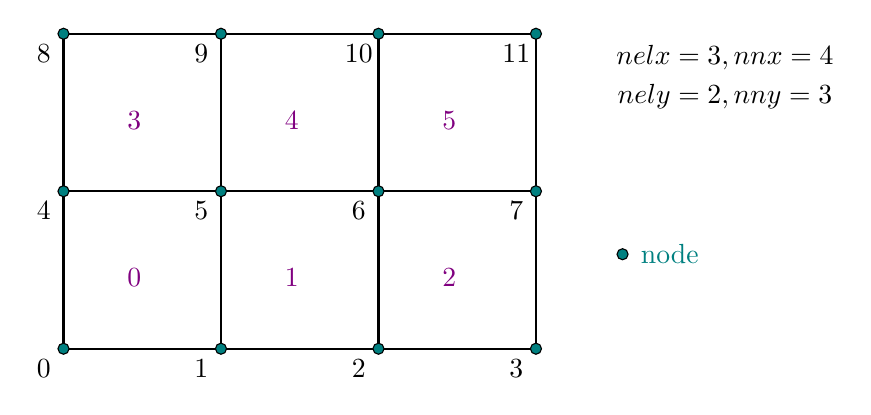
\begin{tikzpicture}
%\draw[step=0.5cm,gray,very thin] (0,0) grid (9,5); %background grid

\draw[thick] (1,1) -- (7,1) -- (7,5) -- (1,5) -- cycle;  
\draw[thick] (1,3) -- (7,3) ;
\draw[thick] (3,1) -- (3,5) ;
\draw[thick] (5,1) -- (5,5) ;

\draw[black,fill=teal] (1,1)     circle (2pt); 
\draw[black,fill=teal] (3,1)     circle (2pt); 
\draw[black,fill=teal] (5,1)     circle (2pt); 
\draw[black,fill=teal] (7,1)     circle (2pt); 

\draw[black,fill=teal] (1,3)     circle (2pt); 
\draw[black,fill=teal] (3,3)     circle (2pt); 
\draw[black,fill=teal] (5,3)     circle (2pt); 
\draw[black,fill=teal] (7,3)     circle (2pt); 

\draw[black,fill=teal] (1,5)     circle (2pt); 
\draw[black,fill=teal] (3,5)     circle (2pt); 
\draw[black,fill=teal] (5,5)     circle (2pt); 
\draw[black,fill=teal] (7,5)     circle (2pt); 

\node[] at (0.75,0.75) {0};
\node[] at (2.75,0.75) {1};
\node[] at (4.75,0.75) {2};
\node[] at (6.75,0.75) {3};

\node[] at (0.75,2.75) {4};
\node[] at (2.75,2.75) {5};
\node[] at (4.75,2.75) {6};
\node[] at (6.75,2.75) {7};

\node[] at (0.75,4.75) {8};
\node[] at (2.75,4.75) {9};
\node[] at (4.75,4.75) {10};
\node[] at (6.75,4.75) {11};

\node[violet] at (1.9,1.9) {0};
\node[violet] at (3.9,1.9) {1};
\node[violet] at (5.9,1.9) {2};
\node[violet] at (1.9,3.9) {3};
\node[violet] at (3.9,3.9) {4};
\node[violet] at (5.9,3.9) {5};

\draw[black,fill=teal] (8.1,2.2) circle (2pt); 
\node[] at (8.7,2.2) {{\color{teal}node}};

\node[] at (9.4,4.7) {$nelx=3, nnx=4$};
\node[] at (9.4,4.2) {$nely=2, nny=3$};

\end{tikzpicture}

\end{center}

\noindent In the case there is only a single degree of freedom per node, the 
assembled FEM matrix ${\bm M}$ will look like this:
\[
{\bm M}=
\left(
\begin{array}{cccccccccccc}
\Box & \Box &      &      & \Box & \Box &      &      &      &      &      &      \\
\Box & \Box & \Box &      & \Box & \Box & \Box &      &      &      &      &      \\
     & \Box & \Box & \Box &      & \Box & \Box & \Box &      &      &      &      \\
     &      & \Box & \Box &      &      & \Box & \Box &      &      &      &      \\
\Box & \Box &      &      & \Box & \Box &      &      & \Box & \Box &      &      \\
\Box & \Box & \Box &      & \Box & \Box & \Box &      & \Box & \Box & \Box &      \\
     & \Box & \Box & \Box &      & \Box & \Box & \Box &      & \Box & \Box & \Box \\
     &      & \Box & \Box &      &      & \Box & \Box &      &      & \Box & \Box \\
     &      &      &      & \Box & \Box &      &      & \Box & \Box &      &      \\
     &      &      &      & \Box & \Box & \Box &      & \Box & \Box & \Box &      \\
     &      &      &      &      & \Box & \Box & \Box &      & \Box & \Box & \Box \\
     &      &      &      &      &      & \Box & \Box &      &      & \Box & \Box 
\end{array}
\right)
\]
where the $\Box$ stand for non-zero terms.
This matrix structure stems from the fact that
\begin{itemize}
\item node 0 sees nodes 0,1,4,5 (1st line/column of the matrix)
\item node 1 sees nodes 0,1,2,4,5,6 (2nd line/column of the matrix)
\item node 2 sees nodes 1,2,3,5,6,7 (3rd line/column of the matrix)
\item node 3 sees nodes 2,3,6,7
\item node 4 sees nodes 0,1,4,5,8,9
\item node 5 sees nodes 0,1,2,4,5,6,8,9,10 
\item node 6 sees nodes 1,2,3,5,6,7,9,10,11
\item node 7 sees nodes 2,3,6,7,10,11
\item node 8 sees nodes 4,5,8,9
\item node 9 sees nodes 4,5,6,8,9,10
\item node 10 sees nodes 5,6,7,9,10,11 
\item node 11 sees nodes 6,7,10,11 (last line/column of the matrix)
\end{itemize}
In light thereof, we have
\begin{itemize}
\item 4 corner nodes which have 4 neighbours (counting themselves) 
\item 2(nnx-2) nodes which have 6 neighbours
\item 2(nny-2) nodes which have 6 neighbours
\item (nnx-2)$\times$(nny-2) nodes which have 9 neighbours
\end{itemize}
In total, the number of non-zero terms in the matrix above is then:
\[
NZ=4\times4+4\times6+2\times6+2\times9=70
\]
and in general, we would then have:
\[
NZ=4\times4+[2(nnx-2)+2(nny-2)]\times6 + (nnx-2)(nny-2)\times9
\]
Let us temporarily assume $nnx=nny=n$. The matrix size (total
number of unknowns) is then $N=n^2$ and  
\[
NZ=16+24(n-2)+9(n-2)^2
\]
A full matrix array would contain $N^2=n^4$ terms. 
The ratio of $NZ$ (the actual number of reals to store)
to the full matrix size (the number of reals a full matrix contains) is then 
\[
R = \frac{16+24(n-2)+9(n-2)^2}{n^4}
\]
It is then obvious that when $n$ is large enough $R \sim 1/n^2$.

CSR stores the nonzeros of the matrix row by row, in a
single indexed array A of double precision  numbers.
Another array COLIND contains the column index of each
corresponding entry in the A array. A third integer array RWPTR
contains pointers to the beginning of each row, which an additional pointer to
the first index following the nonzeros of the matrix A.
A and COLIND have length NZ and RWPTR has length N+1.

In the case of the here-above matrix, the arrays COLIND and RWPTR will look like:
\begin{eqnarray}
COLIND&=&(0,1,4,5, \; 0,1,2,4,5,6, \; 1,2,3,5,6,7, ..., 6,7,10,11) \nn\\
RWPTR &=&(0,4,10,16, ... )   \nn
\end{eqnarray}


%..............................................................................
\subsection{2D domain - $Q_1$ - Symmetric matrix CSR storage} \label{ss:symmcsrss}

If the matrix is symmetric, i.e. ${\bm M}={\bm M}^T$, then we may wish to 
only store half of it, always in the interest of saving memory. 
Only the following remaining $\Box$ entries are relevant now:
\[
{\bm M}=
\left(
\begin{array}{cccccccccccc}
\Box & \Box &      &      & \Box & \Box &      &      &      &      &      &      \\
     & \Box & \Box &      & \Box & \Box & \Box &      &      &      &      &      \\
     &      & \Box & \Box &      & \Box & \Box & \Box &      &      &      &      \\
     &      &      & \Box &      &      & \Box & \Box &      &      &      &      \\
     &      &      &      & \Box & \Box &      &      & \Box & \Box &      &      \\
     &      &      &      &      & \Box & \Box &      & \Box & \Box & \Box &      \\
     &      &      &      &      &      & \Box & \Box &      & \Box & \Box & \Box \\
     &      &      &      &      &      &      & \Box &      &      & \Box & \Box \\
     &      &      &      &      &      &      &      & \Box & \Box &      &      \\
     &      &      &      &      &      &      &      &      & \Box & \Box &      \\
     &      &      &      &      &      &      &      &      &      & \Box & \Box \\
     &      &      &      &      &      &      &      &      &      &      & \Box 
\end{array}
\right)
\]
We see that the number of nonzeros is now 
\[
NZ_{symm}= \frac{NZ-n}{2}+n
\]
and in this case $NZ_{symm}=(70-12)/2+12=41$.
Then 
\begin{eqnarray}
COLIND&=&(0,1,4,5, \; 1,2,4,5,6, \; 3,5,6,7, ..., ,11) \nn\\
RWPTR &=&(0,4,9,14, ... )   \nn
\end{eqnarray}

In case the numbering is Fortran-like, then 
\begin{eqnarray}
ja=COLIND&=&(
1, 2, 5, 6, \quad  2, 3, 5, 6, 7, \quad 3, 4, 6, 7, 8, \quad      
4, 7, 8, \quad  5, 6, 9, 10, \quad 6, 7, 9, 10, 11, \nn\\
&& 7, 8, 10, 11, 12, \quad 8, 11, 12, \quad 9, 10, \quad 10, 11, \quad  11, 12, \quad 12) \nn\\
ia=RWPTR &=&(1, 5, 10, 15, 18, 22, 27, 32, 35, 37, 39, 41, 42)  \nn
\end{eqnarray}

%..............................................................................
\subsection{2D domain - $Q_1$ - Two degrees of freedom per node}

When there are now two degrees of freedom per node, such as in the case 
of the Stokes equation in two-dimensions, the size of the $\K$ matrix 
is given $NfemV=nnx*nny*ndofV$ where $NfemV$ is the total number of 
velocity degrees of freedom.

\begin{center}
\input{tikz/tikz_3x2_two}
\end{center}

In the case of the small grid above, we have then $NfemV=24$ and
elemental matrices are now $8\times8$ in size.

We still have
\begin{itemize}
\item $4$ corner nodes which have 4 neighbours
\item $2(nnx-2)$ nodes which have 6 neighbours
\item $2(nny-2)$ nodes which have 6 neighbours
\item $(nnx-2)\cdot(nny-2)$ nodes which have 9 neighbours,
\end{itemize}
but now each degree of freedom from a node sees the other two
degrees of freedom of another node too.
In that case, the number of nonzeros has been multiplied by four
and the assembled FEM matrix looks like:
\begin{equation}
\left(
\begin{array}{cccccccccccccccccccccccc}
\Box&\Box & \Box&\Box &  &  &  &  & \Box&\Box & \Box&\Box &  &  &  &  &  &  &  &  &  &  &  &  \\
\Box&\Box & \Box&\Box &  &  &  &  & \Box&\Box & \Box&\Box &  &  &  &  &  &  &  &  &  &  &  &  \\
\Box&\Box & \Box&\Box & \Box&\Box &  &  & \Box&\Box & \Box&\Box & \Box&\Box &  &  &  &  &  &  &  &  &  &  \\
\Box&\Box & \Box&\Box & \Box&\Box &  &  & \Box&\Box & \Box&\Box & \Box&\Box &  &  &  &  &  &  &  &  &  &  \\
 &  & \Box&\Box & \Box&\Box & \Box&\Box &  &  & \Box&\Box & \Box&\Box & \Box&\Box &  &  &  &  &  &  &  &  \\
 &  & \Box&\Box & \Box&\Box & \Box&\Box &  &  & \Box&\Box & \Box&\Box & \Box&\Box &  &  &  &  &  &  &  &  \\
 &  &  &  & \Box&\Box & \Box&\Box &  &  &  &  & \Box&\Box & \Box&\Box &  &  &  &  &  &  &  &  \\
 &  &  &  & \Box&\Box & \Box&\Box &  &  &  &  & \Box&\Box & \Box&\Box &  &  &  &  &  &  &  &  \\
\Box&\Box & \Box&\Box &  &  &  &  & \Box&\Box & \Box&\Box &  &  &  &  & \Box&\Box & \Box&\Box &  &  &  &  \\
\Box&\Box & \Box&\Box &  &  &  &  & \Box&\Box & \Box&\Box &  &  &  &  & \Box&\Box & \Box&\Box &  &  &  &  \\
\Box&\Box & \Box&\Box & \Box&\Box &  &  & \Box&\Box & \Box&\Box & \Box&\Box &  &  & \Box&\Box & \Box&\Box & \Box&\Box &  &  \\
\Box&\Box & \Box&\Box & \Box&\Box &  &  & \Box&\Box & \Box&\Box & \Box&\Box &  &  & \Box&\Box & \Box&\Box & \Box&\Box &  &  \\
 &  & \Box&\Box & \Box&\Box & \Box&\Box &  &  & \Box&\Box & \Box&\Box & \Box&\Box &  &  & \Box&\Box & \Box&\Box & \Box&\Box \\
 &  & \Box&\Box & \Box&\Box & \Box&\Box &  &  & \Box&\Box & \Box&\Box & \Box&\Box &  &  & \Box&\Box & \Box&\Box & \Box&\Box \\
 &  &  &  & \Box&\Box & \Box&\Box &  &  &  &  & \Box&\Box & \Box&\Box &  &  &  &  & \Box&\Box & \Box&\Box \\
 &  &  &  & \Box&\Box & \Box&\Box &  &  &  &  & \Box&\Box & \Box&\Box &  &  &  &  & \Box&\Box & \Box&\Box \\
 &  &  &  &  &  &  &  & \Box&\Box & \Box&\Box &  &  &  &  & \Box&\Box & \Box&\Box &  &  &  &  \\
 &  &  &  &  &  &  &  & \Box&\Box & \Box&\Box &  &  &  &  & \Box&\Box & \Box&\Box &  &  &  &  \\
 &  &  &  &  &  &  &  & \Box&\Box & \Box&\Box & \Box&\Box &  &  & \Box&\Box & \Box&\Box & \Box&\Box &  &  \\
 &  &  &  &  &  &  &  & \Box&\Box & \Box&\Box & \Box&\Box &  &  & \Box&\Box & \Box&\Box & \Box&\Box &  &  \\
 &  &  &  &  &  &  &  &  &  & \Box&\Box & \Box&\Box & \Box&\Box &  &  & \Box&\Box & \Box&\Box & \Box&\Box \\
 &  &  &  &  &  &  &  &  &  & \Box&\Box & \Box&\Box & \Box&\Box &  &  & \Box&\Box & \Box&\Box & \Box&\Box \\
 &  &  &  &  &  &  &  &  &  &  &  & \Box&\Box & \Box&\Box &  &  &  &  & \Box&\Box & \Box&\Box \\
 &  &  &  &  &  &  &  &  &  &  &  & \Box&\Box & \Box&\Box &  &  &  &  & \Box&\Box & \Box&\Box 
\end{array}
\right)\nonumber
\end{equation}
Note that the degrees of freedom are organised as follows: 
\[
(u_0,v_0,u_1,v_1,u_2,v_2, ... u_{11},v_{11})
\]
In general, we would then have:
\[
NZ=4 \left[4\times4+[2(nnx-2)+2(nny-2)]\times6 + (nnx-2)(nny-2)\times9 \right]
\]
and in the case of the small grid,
the number of non-zero terms in the matrix is then:
\[
NZ=4\left[4\times4+4\times6+2\times6+2\times9\right]=280
\]
In the case of the here-above matrix, the arrays COLIND and RWPTR will look like:
\begin{eqnarray}
COLIND&=&(0,1,2,3,8,9,10,11, \; 0,1,2,3,8,9,10,11,\; ...) \nn\\
RWPTR &=&(0,8,16,28, ... ) \nn
\end{eqnarray}

Assuming we are using $Q_1\times P_0$ elements, the structure of the matrix $\G_{el}^T$ is as follows
(the 6 pressure dofs are connected to 24 velocity dofs):

\begin{scriptsize}
\begin{equation}
\left(
\begin{array}{ccccccccccccccccccccccccc}
&0 & 1 & 2 & 3 & 4 & 5 & 6 & 7 & 8 & 9 & 10 & 11 & 12 & 13 & 14 & 15 & 16 & 17 & 18 & 19 & 20 & 21 & 22 & 23     \\
\Box&\Box & \Box&\Box &  &  &  &  & \Box&\Box & \Box&\Box &  &  &  &  &  &  &  &  &  &  &  &  \\
    &     & \Box&\Box & \Box&\Box &  &  &  &  & \Box&\Box & \Box&\Box &  &  &  &  &  &  &  &  &  &  \\
 & &     &     & \Box&\Box & \Box&\Box &  &  &  &  & \Box&\Box & \Box&\Box &  &  &  &  &  &  &  &    \\
 & & & &  & &     &     & \Box&\Box & \Box&\Box &  &  &  &  & \Box&\Box & \Box&\Box &  &  &  &      \\
 & & & & & &  & &     &     & \Box&\Box & \Box&\Box &  &  &  &  & \Box&\Box & \Box&\Box &  &       \\
 & &  & & & & & &  & &     &     & \Box&\Box & \Box&\Box &  &  &  &  & \Box&\Box & \Box&\Box        
\end{array}
\right)
\end{equation} 
\end{scriptsize}

\begin{center}
\input{tikz/csrStokes_3x2_ELEFANT}
\input{tikz/csrStokes_4x3_ELEFANT}
\input{tikz/csrStokes_5x4_ELEFANT}\\
{\captionfont From left to right: Nonzero structures of the assembled Stokes matrix for a 
$3\times 2$, $4\times 3$ and $5\times 4$ mesh of $Q_1\times P_0$ elements.}
\end{center}


Assuming we are now using $Q_1\times Q_1$ elements (without bubble), 
the structure of the matrix $\G_{el}^T$ is different: we now have 12 pressure dofs 
which are coupled to 24 velocity dofs:
\begin{scriptsize}
\begin{equation}
\left(
\begin{array}{ccccccccccccccccccccccccc}
 & 1 & 2 & 3 & 4 & 5 & 6 & 7 & 8 & 9 & 10 & 11 & 12 & 13 & 14 & 15 & 16 & 17 & 18 & 19 & 20 & 21 & 22 & 23 & 24    \\
0 &\Box&\Box & \Box&\Box &  &  &  &  & \Box&\Box & \Box&\Box &  &  &  &  &  &  &  &  &  &  &  &  \\
1 & \Box&\Box & \Box&\Box & \Box  & \Box  &  &  & \Box&\Box & \Box&\Box & \Box  & \Box  &  &  &  &  &  &  &  &  &  & \\
2 &  & & \Box&\Box & \Box  & \Box  & \Box  & \Box  & & & \Box&\Box & \Box  & \Box  & \Box  &\Box  &  &  &  &  &  &  &  & \\ 
3 &  & & &  & \Box  & \Box  & \Box  & \Box  & & & & & \Box  & \Box  & \Box  &\Box  &  &  &  &  &  &  &  & \\ 
\\
... \\
\\
9 & & & & & & & & &\Box &\Box &\Box &\Box & \Box  & \Box &  &  & & &\Box &\Box & \Box &\Box & &  \\
10 & & & & & & & & & & &\Box &\Box & \Box  & \Box & \Box & \Box & & &\Box &\Box & \Box &\Box &\Box & \Box \\
11 & & & & & & & & & & & & & \Box  & \Box & \Box & \Box & & & & & \Box &\Box &\Box & \Box \\
\end{array}
\right)
\end{equation} 
\end{scriptsize}

%..............................................................................
\subsection{2D domain - $Q_2$ - Two degrees of freedom per node}


When there are now two degrees of freedom per node, such as in the case 
of the Stokes equation in two-dimensions, the size of the $\K$ matrix 
is given $NfemV=nnx*nny*ndofV$ where $NfemV$ is the total number of 
velocity degrees of freedom. What is different here is that for $Q_2$
elements we have $nnx=2*nelx+1$ and $nny=2*nely+1$.

\begin{center}
\begin{flushright} {\tiny {\color{gray} (tikz\_3x2\_two\_Q2.tex)}} \end{flushright}
%~~~~~~~~~~~~~~~~~~~~~~~~~~~~~~~~~~~~~~~~~~~~~~~~~~~~~~~~~~~~~~~~~~~~~~~~~~~~~~~~~~~~~~~~~~~~~~~~~~

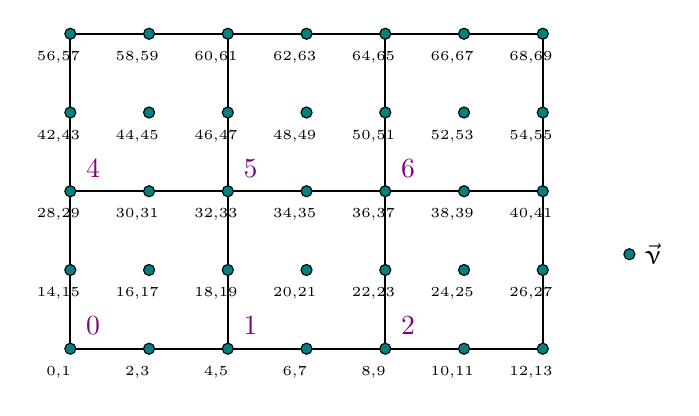
\begin{tikzpicture}
%\draw[step=0.5cm,gray,very thin] (0,0) grid (8,6); %background grid

\draw[thick] (1,1) -- (7,1) -- (7,5) -- (1,5) -- cycle;  
\draw[thick] (1,3) -- (7,3) ;
\draw[thick] (3,1) -- (3,5) ;
\draw[thick] (5,1) -- (5,5) ;

\draw[black,fill=teal] (1,1)     circle (2pt); 
\draw[black,fill=teal] (2,1)     circle (2pt); 
\draw[black,fill=teal] (3,1)     circle (2pt); 
\draw[black,fill=teal] (4,1)     circle (2pt); 
\draw[black,fill=teal] (5,1)     circle (2pt); 
\draw[black,fill=teal] (6,1)     circle (2pt); 
\draw[black,fill=teal] (7,1)     circle (2pt); 

\draw[black,fill=teal] (1,2)     circle (2pt); 
\draw[black,fill=teal] (2,2)     circle (2pt); 
\draw[black,fill=teal] (3,2)     circle (2pt); 
\draw[black,fill=teal] (4,2)     circle (2pt); 
\draw[black,fill=teal] (5,2)     circle (2pt); 
\draw[black,fill=teal] (6,2)     circle (2pt); 
\draw[black,fill=teal] (7,2)     circle (2pt); 

\draw[black,fill=teal] (1,3)     circle (2pt); 
\draw[black,fill=teal] (2,3)     circle (2pt); 
\draw[black,fill=teal] (3,3)     circle (2pt); 
\draw[black,fill=teal] (4,3)     circle (2pt); 
\draw[black,fill=teal] (5,3)     circle (2pt); 
\draw[black,fill=teal] (6,3)     circle (2pt); 
\draw[black,fill=teal] (7,3)     circle (2pt); 

\draw[black,fill=teal] (1,4)     circle (2pt); 
\draw[black,fill=teal] (2,4)     circle (2pt); 
\draw[black,fill=teal] (3,4)     circle (2pt); 
\draw[black,fill=teal] (4,4)     circle (2pt); 
\draw[black,fill=teal] (5,4)     circle (2pt); 
\draw[black,fill=teal] (6,4)     circle (2pt); 
\draw[black,fill=teal] (7,4)     circle (2pt); 

\draw[black,fill=teal] (1,5)     circle (2pt); 
\draw[black,fill=teal] (2,5)     circle (2pt); 
\draw[black,fill=teal] (3,5)     circle (2pt); 
\draw[black,fill=teal] (4,5)     circle (2pt); 
\draw[black,fill=teal] (5,5)     circle (2pt); 
\draw[black,fill=teal] (6,5)     circle (2pt); 
\draw[black,fill=teal] (7,5)     circle (2pt); 

\node[] at (0.85,0.7) {\tiny 0,1};
\node[] at (1.85,0.7) {\tiny 2,3};
\node[] at (2.85,0.7) {\tiny 4,5};
\node[] at (3.85,0.7) {\tiny 6,7};
\node[] at (4.85,0.7) {\tiny 8,9};
\node[] at (5.85,0.7) {\tiny 10,11};
\node[] at (6.85,0.7) {\tiny 12,13};

\node[] at (0.85,1.7) {\tiny 14,15};
\node[] at (1.85,1.7) {\tiny 16,17};
\node[] at (2.85,1.7) {\tiny 18,19};
\node[] at (3.85,1.7) {\tiny 20,21};
\node[] at (4.85,1.7) {\tiny 22,23};
\node[] at (5.85,1.7) {\tiny 24,25};
\node[] at (6.85,1.7) {\tiny 26,27};

\node[] at (0.85,2.7) {\tiny 28,29}; 
\node[] at (1.85,2.7) {\tiny 30,31}; 
\node[] at (2.85,2.7) {\tiny 32,33}; 
\node[] at (3.85,2.7) {\tiny 34,35}; 
\node[] at (4.85,2.7) {\tiny 36,37}; 
\node[] at (5.85,2.7) {\tiny 38,39}; 
\node[] at (6.85,2.7) {\tiny 40,41}; 

\node[] at (0.85,3.7) {\tiny 42,43}; 
\node[] at (1.85,3.7) {\tiny 44,45}; 
\node[] at (2.85,3.7) {\tiny 46,47}; 
\node[] at (3.85,3.7) {\tiny 48,49}; 
\node[] at (4.85,3.7) {\tiny 50,51}; 
\node[] at (5.85,3.7) {\tiny 52,53}; 
\node[] at (6.85,3.7) {\tiny 54,55}; 

\node[] at (0.85,4.7) {\tiny 56,57}; 
\node[] at (1.85,4.7) {\tiny 58,59}; 
\node[] at (2.85,4.7) {\tiny 60,61}; 
\node[] at (3.85,4.7) {\tiny 62,63}; 
\node[] at (4.85,4.7) {\tiny 64,65}; 
\node[] at (5.85,4.7) {\tiny 66,67}; 
\node[] at (6.85,4.7) {\tiny 68,69}; 

\node[violet] at (1.29,1.29) {0};
\node[violet] at (3.29,1.29) {1};
\node[violet] at (5.29,1.29) {2};
\node[violet] at (1.29,3.29) {4};
\node[violet] at (3.29,3.29) {5};
\node[violet] at (5.29,3.29) {6};

\draw[black,fill=teal] (8.1,2.2) circle (2pt); 
\node[] at (8.4,2.2) {$\vec\upnu$};

\end{tikzpicture}


\end{center}

In the case of the small grid above, we have then 
$nelx=3$, $nely=2$, so that $nnx=7$ and $nny=5$, and then
$NfemV=7*5*2=70$ and elemental matrices are now $18\times18$ in size.


\begin{center}
\begin{flushright} {\tiny {\color{gray} (tikz\_3x2\_Q2.tex)}} \end{flushright}
%~~~~~~~~~~~~~~~~~~~~~~~~~~~~~~~~~~~~~~~~~~~~~~~~~~~~~~~~~~~~~~~~~~~~~~~~~~~~~~~~~~~~~~~~~~~~~~~~~~

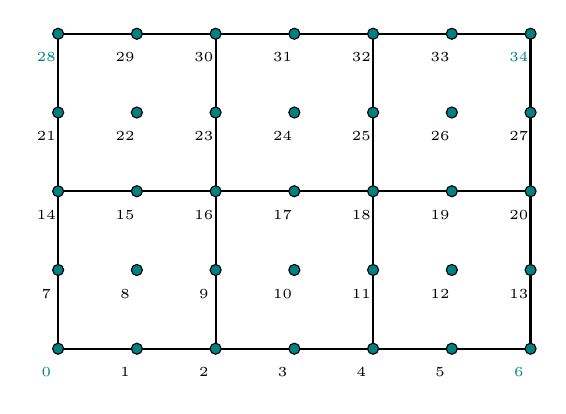
\begin{tikzpicture}
%\draw[step=0.5cm,gray,very thin] (0,0) grid (8,6); %background grid

\draw[thick] (1,1) -- (7,1) -- (7,5) -- (1,5) -- cycle;  
\draw[thick] (1,3) -- (7,3) ;
\draw[thick] (3,1) -- (3,5) ;
\draw[thick] (5,1) -- (5,5) ;

\draw[black,fill=teal] (1,1)     circle (2pt); 
\draw[black,fill=teal] (2,1)     circle (2pt); 
\draw[black,fill=teal] (3,1)     circle (2pt); 
\draw[black,fill=teal] (4,1)     circle (2pt); 
\draw[black,fill=teal] (5,1)     circle (2pt); 
\draw[black,fill=teal] (6,1)     circle (2pt); 
\draw[black,fill=teal] (7,1)     circle (2pt); 

\draw[black,fill=teal] (1,2)     circle (2pt); 
\draw[black,fill=teal] (2,2)     circle (2pt); 
\draw[black,fill=teal] (3,2)     circle (2pt); 
\draw[black,fill=teal] (4,2)     circle (2pt); 
\draw[black,fill=teal] (5,2)     circle (2pt); 
\draw[black,fill=teal] (6,2)     circle (2pt); 
\draw[black,fill=teal] (7,2)     circle (2pt); 

\draw[black,fill=teal] (1,3)     circle (2pt); 
\draw[black,fill=teal] (2,3)     circle (2pt); 
\draw[black,fill=teal] (3,3)     circle (2pt); 
\draw[black,fill=teal] (4,3)     circle (2pt); 
\draw[black,fill=teal] (5,3)     circle (2pt); 
\draw[black,fill=teal] (6,3)     circle (2pt); 
\draw[black,fill=teal] (7,3)     circle (2pt); 

\draw[black,fill=teal] (1,4)     circle (2pt); 
\draw[black,fill=teal] (2,4)     circle (2pt); 
\draw[black,fill=teal] (3,4)     circle (2pt); 
\draw[black,fill=teal] (4,4)     circle (2pt); 
\draw[black,fill=teal] (5,4)     circle (2pt); 
\draw[black,fill=teal] (6,4)     circle (2pt); 
\draw[black,fill=teal] (7,4)     circle (2pt); 

\draw[black,fill=teal] (1,5)     circle (2pt); 
\draw[black,fill=teal] (2,5)     circle (2pt); 
\draw[black,fill=teal] (3,5)     circle (2pt); 
\draw[black,fill=teal] (4,5)     circle (2pt); 
\draw[black,fill=teal] (5,5)     circle (2pt); 
\draw[black,fill=teal] (6,5)     circle (2pt); 
\draw[black,fill=teal] (7,5)     circle (2pt); 

\node[] at (0.85,0.7) {\tiny \color{teal} 0};
\node[] at (1.85,0.7) {\tiny 1};
\node[] at (2.85,0.7) {\tiny 2};
\node[] at (3.85,0.7) {\tiny 3};
\node[] at (4.85,0.7) {\tiny 4};
\node[] at (5.85,0.7) {\tiny 5};
\node[] at (6.85,0.7) {\tiny \color{teal} 6};

\node[] at (0.85,1.7) {\tiny 7};
\node[] at (1.85,1.7) {\tiny 8};
\node[] at (2.85,1.7) {\tiny 9};
\node[] at (3.85,1.7) {\tiny 10};
\node[] at (4.85,1.7) {\tiny 11};
\node[] at (5.85,1.7) {\tiny 12};
\node[] at (6.85,1.7) {\tiny 13};

\node[] at (0.85,2.7) {\tiny 14}; 
\node[] at (1.85,2.7) {\tiny 15}; 
\node[] at (2.85,2.7) {\tiny 16}; 
\node[] at (3.85,2.7) {\tiny 17}; 
\node[] at (4.85,2.7) {\tiny 18}; 
\node[] at (5.85,2.7) {\tiny 19}; 
\node[] at (6.85,2.7) {\tiny 20}; 

\node[] at (0.85,3.7) {\tiny 21}; 
\node[] at (1.85,3.7) {\tiny 22}; 
\node[] at (2.85,3.7) {\tiny 23}; 
\node[] at (3.85,3.7) {\tiny 24}; 
\node[] at (4.85,3.7) {\tiny 25}; 
\node[] at (5.85,3.7) {\tiny 26}; 
\node[] at (6.85,3.7) {\tiny 27}; 

\node[] at (0.85,4.7) {\tiny \color{teal} 28}; 
\node[] at (1.85,4.7) {\tiny 29}; 
\node[] at (2.85,4.7) {\tiny 30}; 
\node[] at (3.85,4.7) {\tiny 31}; 
\node[] at (4.85,4.7) {\tiny 32}; 
\node[] at (5.85,4.7) {\tiny 33}; 
\node[] at (6.85,4.7) {\tiny \color{teal} 34}; 

\end{tikzpicture}


\end{center}


Concretely here:
\begin{itemize}
\item nodes {\color{teal} 0,6,28,34} see 9 nodes (corners)
\item nodes 1,3,5,7,8,10,12,13,21,22,24,26,27,29,31,33 see 9 nodes
\item nodes 2,4,9,11,14,15,17,19,20,23,25,30,32, see 15 nodes
\item nodes 16,18 see 25 nodes
\end{itemize}

If there was only one dof per node, we would find 
the number of non zeros as follow:
\[
NZ=4*9 + 16*9 + 13*15 + 2*25 = 36+144 + 195 + 50 = 425
\]
But since there are two velocity dofs per node, we find that 
the total number of nonzeros is 4 times higher, i.e.
\[
NZ=1700
\] 
And if we choose for a symmetric CSR storage:
\[
NZ_{symm} = \frac{NZ-n}{2}+n = \frac{1700-70}{2} + 70 = 885 
\]

Let us now turn to the real case of 2 dofs per node and establish 
who sees who:

\begin{tabular}{lp{14.5cm}l}
dof &  sees other dofs & total\\
\hline
0 & 0,1,2,3,4,5,14,15,16,17,18,19,28,29,30,31,32,33 & 18 \\
1 & 0,1,2,3,4,5,14,15,16,17,18,19,28,29,30,31,32,33 & 18 \\
2 & 0,1,2,3,4,5,14,15,16,17,18,19,28,29,30,31,32,33 & 18 \\
3 & 0,1,2,3,4,5,14,15,16,17,18,19,28,29,30,31,32,33 & 18 \\
4 & 0,1,2,3,4,5,6,7,8,9,14,15,16,17,18,19,20,21,22,23,28,29,30,31,32,33,34,35,36,37 & 30 \\
5 & 0,1,2,3,4,5,6,7,8,9,14,15,16,17,18,19,20,21,22,23,28,29,30,31,32,33,34,35,36,37 & 30 \\
6 & 4,5,6,7,8,9,18,19,20,21,22,23,32,33,34,35,36,37 & 18 \\
7 & 4,5,6,7,8,9,18,19,20,21,22,23,32,33,34,35,36,37 & 18 \\
8 & 4,5,6,7,8,9,10,11,12,13,18,19,20,21,22,23,24,25,26,27,32,33,34,35,36,37,38,39,40,41 & 30 \\
9 & 4,5,6,7,8,9,10,11,12,13,18,19,20,21,22,23,24,25,26,27,32,33,34,35,36,37,38,39,40,41 & 30 \\
10 & 8,9,10,11,12,13,22,23,24,25,26,27,36,37,38,39,40,41 & 18\\
11 & 8,9,10,11,12,13,22,23,24,25,26,27,36,37,38,39,40,41 & 18\\
12 & 8,9,10,11,12,13,22,23,24,25,26,27,36,37,38,39,40,41 & 18\\
13 & 8,9,10,11,12,13,22,23,24,25,26,27,36,37,38,39,40,41 & 18\\
14 & 0,1,2,3,4,5,14,15,16,17,18,19,28,29,30,31,32,33 & 18 \\
15 & 0,1,2,3,4,5,14,15,16,17,18,19,28,29,30,31,32,33 & 18 \\
16 & 0,1,2,3,4,5,14,15,16,17,18,19,28,29,30,31,32,33 & 18 \\
17 & 0,1,2,3,4,5,14,15,16,17,18,19,28,29,30,31,32,33 & 18 \\
 ... & ... & ... \\
68 & 36,37,38,39,50,51,52,53,54,55,64,65,66,67,68,69 & 18 \\
69 & 36,37,38,39,50,51,52,53,54,55,64,65,66,67,68,69 & 18 \\
\hline
\end{tabular}

The second column of this array is the content of the ja array.


In order establish a pattern we will need a bigger mesh:

\begin{center}
\begin{flushright} {\footnotesize {\color{gray} (tikz\_4x3\_Q2.tex)}} \end{flushright}
%~~~~~~~~~~~~~~~~~~~~~~~~~~~~~~~~~~~~~~~~~~~~~~~~~~~~~~~~~~~~~~~~~~~~~~~~~~~~~~~~~~~~~~~~~~~~~~~~~~

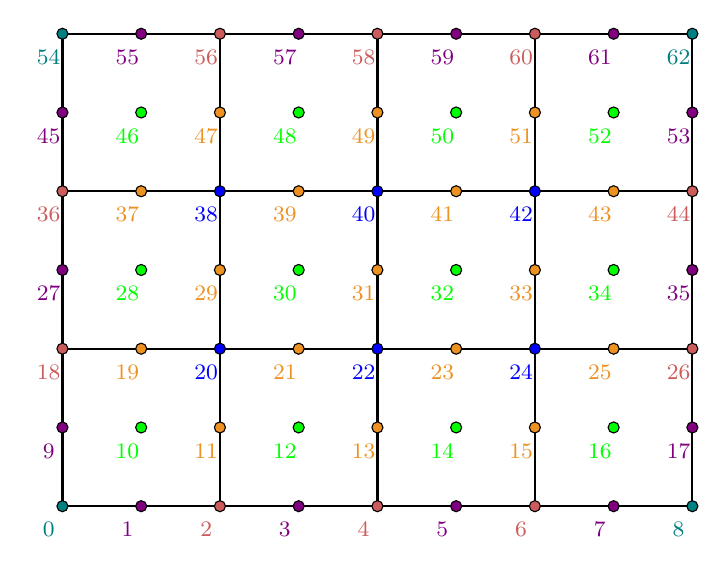
\begin{tikzpicture}
%\draw[step=0.5cm,gray,very thin] (0,0) grid (10,8); %background grid

\draw[thick] (1,1) -- (9,1) -- (9,7) -- (1,7) -- cycle;  
\draw[thick] (1,3) -- (9,3) ;
\draw[thick] (1,5) -- (9,5) ;
\draw[thick] (3,1) -- (3,7) ;
\draw[thick] (5,1) -- (5,7) ;
\draw[thick] (7,1) -- (7,7) ;

\draw[black,fill=teal] (1,1)     circle (2pt);  %0
\draw[black,fill=violet] (2,1)     circle (2pt); 
\draw[black,fill=chestnut] (3,1)     circle (2pt); 
\draw[black,fill=violet] (4,1)     circle (2pt); 
\draw[black,fill=chestnut] (5,1)     circle (2pt); 
\draw[black,fill=violet] (6,1)     circle (2pt); 
\draw[black,fill=chestnut] (7,1)     circle (2pt); 
\draw[black,fill=violet] (8,1)     circle (2pt); 
\draw[black,fill=teal] (9,1)     circle (2pt); %8

\draw[black,fill=violet] (1,2)     circle (2pt); %9
\draw[black,fill=green] (2,2)     circle (2pt); 
\draw[black,fill=carrotorange] (3,2)     circle (2pt); 
\draw[black,fill=green] (4,2)     circle (2pt); 
\draw[black,fill=carrotorange] (5,2)     circle (2pt); 
\draw[black,fill=green] (6,2)     circle (2pt); 
\draw[black,fill=carrotorange] (7,2)     circle (2pt); 
\draw[black,fill=green] (8,2)     circle (2pt); 
\draw[black,fill=violet] (9,2)     circle (2pt); %17

\draw[black,fill=chestnut] (1,3)     circle (2pt); %18
\draw[black,fill=carrotorange] (2,3)     circle (2pt); 
\draw[black,fill=blue] (3,3)     circle (2pt); 
\draw[black,fill=carrotorange] (4,3)     circle (2pt); 
\draw[black,fill=blue] (5,3)     circle (2pt); 
\draw[black,fill=carrotorange] (6,3)     circle (2pt); 
\draw[black,fill=blue] (7,3)     circle (2pt); 
\draw[black,fill=carrotorange] (8,3)     circle (2pt); 
\draw[black,fill=chestnut] (9,3)     circle (2pt); %26

\draw[black,fill=violet] (1,4)     circle (2pt); %27
\draw[black,fill=green] (2,4)     circle (2pt); 
\draw[black,fill=carrotorange] (3,4)     circle (2pt); 
\draw[black,fill=green] (4,4)     circle (2pt); 
\draw[black,fill=carrotorange] (5,4)     circle (2pt); 
\draw[black,fill=green] (6,4)     circle (2pt); 
\draw[black,fill=carrotorange] (7,4)     circle (2pt); 
\draw[black,fill=green] (8,4)     circle (2pt); 
\draw[black,fill=violet] (9,4)     circle (2pt); %35

\draw[black,fill=chestnut] (1,5)     circle (2pt); %36
\draw[black,fill=carrotorange] (2,5)     circle (2pt); 
\draw[black,fill=blue] (3,5)     circle (2pt); 
\draw[black,fill=carrotorange] (4,5)     circle (2pt); 
\draw[black,fill=blue] (5,5)     circle (2pt); 
\draw[black,fill=carrotorange] (6,5)     circle (2pt); 
\draw[black,fill=blue] (7,5)     circle (2pt); 
\draw[black,fill=carrotorange] (8,5)     circle (2pt); 
\draw[black,fill=chestnut] (9,5)     circle (2pt); %44

\draw[black,fill=violet] (1,6)     circle (2pt); %45 
\draw[black,fill=green] (2,6)     circle (2pt); 
\draw[black,fill=carrotorange] (3,6)     circle (2pt); 
\draw[black,fill=green] (4,6)     circle (2pt); 
\draw[black,fill=carrotorange] (5,6)     circle (2pt); 
\draw[black,fill=green] (6,6)     circle (2pt); 
\draw[black,fill=carrotorange] (7,6)     circle (2pt); 
\draw[black,fill=green] (8,6)     circle (2pt); 
\draw[black,fill=violet] (9,6)     circle (2pt); %53

\draw[black,fill=teal] (1,7)     circle (2pt); %54
\draw[black,fill=violet] (2,7)     circle (2pt); 
\draw[black,fill=chestnut] (3,7)     circle (2pt); 
\draw[black,fill=violet] (4,7)     circle (2pt); 
\draw[black,fill=chestnut] (5,7)     circle (2pt); 
\draw[black,fill=violet] (6,7)     circle (2pt); 
\draw[black,fill=chestnut] (7,7)     circle (2pt); 
\draw[black,fill=violet] (8,7)     circle (2pt); 
\draw[black,fill=teal] (9,7)     circle (2pt); %62

\node[] at (0.825,0.7) {\footnotesize \color{teal} 0};
\node[] at (1.825,0.7) {\footnotesize \color{violet} 1};
\node[] at (2.825,0.7) {\footnotesize \color{chestnut} 2};
\node[] at (3.825,0.7) {\footnotesize \color{violet} 3};
\node[] at (4.825,0.7) {\footnotesize \color{chestnut} 4};
\node[] at (5.825,0.7) {\footnotesize \color{violet} 5};
\node[] at (6.825,0.7) {\footnotesize \color{chestnut} 6};
\node[] at (7.825,0.7) {\footnotesize \color{violet} 7};
\node[] at (8.825,0.7) {\footnotesize \color{teal} 8};

\node[] at (0.825,1.7) {\footnotesize \color{violet} 9};
\node[] at (1.825,1.7) {\footnotesize \color{green} 10};
\node[] at (2.825,1.7) {\footnotesize \color{carrotorange}11};
\node[] at (3.825,1.7) {\footnotesize \color{green} 12};
\node[] at (4.825,1.7) {\footnotesize \color{carrotorange}13};
\node[] at (5.825,1.7) {\footnotesize \color{green} 14};
\node[] at (6.825,1.7) {\footnotesize \color{carrotorange}15};
\node[] at (7.825,1.7) {\footnotesize \color{green} 16};
\node[] at (8.825,1.7) {\footnotesize \color{violet} 17};

\node[] at (0.825,2.7) {\footnotesize \color{chestnut} 18}; 
\node[] at (1.825,2.7) {\footnotesize \color{carrotorange} 19}; 
\node[] at (2.825,2.7) {\footnotesize \color{blue} 20}; 
\node[] at (3.825,2.7) {\footnotesize \color{carrotorange} 21}; 
\node[] at (4.825,2.7) {\footnotesize \color{blue} 22}; 
\node[] at (5.825,2.7) {\footnotesize \color{carrotorange} 23}; 
\node[] at (6.825,2.7) {\footnotesize \color{blue} 24}; 
\node[] at (7.825,2.7) {\footnotesize \color{carrotorange} 25}; 
\node[] at (8.825,2.7) {\footnotesize \color{chestnut} 26}; 

\node[] at (0.825,3.7) {\footnotesize \color{violet} 27}; 
\node[] at (1.825,3.7) {\footnotesize \color{green} 28}; 
\node[] at (2.825,3.7) {\footnotesize \color{carrotorange} 29}; 
\node[] at (3.825,3.7) {\footnotesize \color{green} 30}; 
\node[] at (4.825,3.7) {\footnotesize \color{carrotorange} 31}; 
\node[] at (5.825,3.7) {\footnotesize \color{green} 32}; 
\node[] at (6.825,3.7) {\footnotesize \color{carrotorange} 33}; 
\node[] at (7.825,3.7) {\footnotesize \color{green} 34}; 
\node[] at (8.825,3.7) {\footnotesize \color{violet} 35};

\node[] at (0.825,4.7) {\footnotesize \color{chestnut} 36}; 
\node[] at (1.825,4.7) {\footnotesize \color{carrotorange}37}; 
\node[] at (2.825,4.7) {\footnotesize \color{blue} 38}; 
\node[] at (3.825,4.7) {\footnotesize \color{carrotorange}39}; 
\node[] at (4.825,4.7) {\footnotesize \color{blue} 40}; 
\node[] at (5.825,4.7) {\footnotesize \color{carrotorange}41}; 
\node[] at (6.825,4.7) {\footnotesize \color{blue} 42};
\node[] at (7.825,4.7) {\footnotesize \color{carrotorange}43};
\node[] at (8.825,4.7) {\footnotesize \color{chestnut} 44};

\node[] at (0.825,5.7) {\footnotesize \color{violet} 45}; 
\node[] at (1.825,5.7) {\footnotesize \color{green} 46}; 
\node[] at (2.825,5.7) {\footnotesize \color{carrotorange}47}; 
\node[] at (3.825,5.7) {\footnotesize \color{green} 48}; 
\node[] at (4.825,5.7) {\footnotesize \color{carrotorange}49}; 
\node[] at (5.825,5.7) {\footnotesize \color{green} 50}; 
\node[] at (6.825,5.7) {\footnotesize \color{carrotorange}51};
\node[] at (7.825,5.7) {\footnotesize \color{green} 52};
\node[] at (8.825,5.7) {\footnotesize \color{violet} 53};

\node[] at (0.825,6.7) {\footnotesize \color{teal}54}; 
\node[] at (1.825,6.7) {\footnotesize \color{violet} 55}; 
\node[] at (2.825,6.7) {\footnotesize \color{chestnut} 56}; 
\node[] at (3.825,6.7) {\footnotesize \color{violet} 57}; 
\node[] at (4.825,6.7) {\footnotesize \color{chestnut} 58}; 
\node[] at (5.825,6.7) {\footnotesize \color{violet} 59}; 
\node[] at (6.825,6.7) {\footnotesize \color{chestnut} 60};
\node[] at (7.825,6.7) {\footnotesize \color{violet} 61};
\node[] at (8.825,6.7) {\footnotesize \color{teal} 62};

\end{tikzpicture}

\end{center}



We have
\begin{itemize}
\item {\color{teal} 4} corner nodes which have 9 neighbours
\item {\color{green} $nel$} mid-element nodes which have 9 neighbours
\item {\color{violet} $2*nelx+2*nely$} mid-edge nodes on sides which have 9 neighbours
\item {\color{carrotorange} $(nelx-1)*nely+nelx*(nely-1)$} internal mid-edges nodes which have 15 neighbours
\item {\color{chestnut} $2*(nelx-1)+2*(nely-1)$} side nodes that have 15 neighbours 
\item {\color{blue} $(nelx-1)*(nely-1)$} nodes which have 25 neighbours
\end{itemize}
In the end, the number of non-zeros ($Q_1$) is given by
\begin{eqnarray}
NZ 
&=& {\color{teal} 4 }*9 \nn\\
&+& {\color{green} nel }*9 \nn\\
&+& {\color{violet} (2*nelx+2*nely) }*9 \nn\\
&+& {\color{carrotorange} [(nelx-1)*nely+nelx*(nely-1)] }*15 \nn\\
&+& {\color{chestnut} [2*(nelx-1)+2*(nely-1)] }*15 \nn\\
&+& {\color{blue} (nelx-1)*(nely-1) }*25 \nn
\end{eqnarray}
Verification: $nelx=3$, $nely=2$:
\begin{eqnarray}
NZ
&=& 4*9 + 6*9 + (2*3+2*2)*9 + [(3-1)*2+3*(2-1)]*15
+ [2*(3-1)+2*(2-1)]*15 + (3-1)*(2-1)*25 \nn\\
&=& 36 + 54 + 10*9 + 7*15 + 6*15 + 2*25 \nn\\
&=& 36 + 54 + 90 + 105 + 90 + 50  \nn\\
&=& 425 \nn
\end{eqnarray}
as expected.








%..............................................................................
\subsection{3D domain - $Q_1$ - CSR storage - One degree of freedom}

Let us consider a $3\times4\times2$ grid which counts 
$nnx\cdot nny \cdot nnz = 5 \cdot 4\cdot 3=60$ nodes.
The assembled FEM matrix $\K$ size is then 
$N=nnx\times nny\times nnz \times ndof=180$.

\begin{center}
\input{tikz/tikz_4x3x2.tex}
\end{center}



The total number of nonzeros in the case $ndof=1$ would be decomposed as follows:
\begin{itemize}
\item 8 corners 'see' 8 neighbours
\item 4 edges with $(nnx-2)$ nodes in the x direction see 12 nodes
\item 4 edges with $(nny-2)$ nodes in the y direction see 12 nodes
\item 4 edges with $(nnz-2)$ nodes in the z direction see 12 nodes
\item $2(nnx-2)(nny-2)$ nodes see 18 nodes
\item $2(nnx-2)(nnz-2)$ nodes see 18 nodes
\item $2(nny-2)(nnz-2)$ nodes see 18 nodes
\item $(nnx-2)(nny-2)(nnz-2)$ interior nodes see 27 nodes
\end{itemize}

%..............................................................................
\subsection{3D domain - $Q_2$ - CSR storage - one degree of freedom}


\begin{center}
\input{tikz/tikz_4x3x2_q2.tex}
\end{center}





%..............................................................................
\subsection{Matrix Storage in fieldstone}

The majority of the early codes have the FE matrix being a full array
\begin{lstlisting}
a_mat = np.zeros((Nfem,Nfem),dtype=np.float64) 
\end{lstlisting}
and it is converted to CSR format on the fly in the solve phase:
\begin{lstlisting}
sol = sps.linalg.spsolve(sps.csr_matrix(a_mat),rhs)
\end{lstlisting}

Note that linked list storages can be used (lil\_matrix). Substantial memory savings 
but much longer compute times since it takes longer to write in such arrays.
A conversion to CSR format is still necessary before calling the solver.




%..............................................................................
\subsection{About Sparse Matrix-Vector multiplication} \label{ss:spmv}
\index{general}{SpMV} \index{general}{Sparse Matrix-Vector Multiplication}

When/if the matrix ${\bm M}$ is stored in a two-dimensional array, 
its (left or right) multiplication by a vector is trivial. 
Either one resorts to writing a double for loop (not recommended), 
either one uses {\tt numpy.dot}\footnote{\url{https://numpy.org/doc/stable/reference/generated/numpy.dot.html}}
in python, or {\tt matmul} in Fortran.

However, when the matrix is stored as a single continuous array, say CSR, how does this work?
This question is {\it very important} since iterative solvers such as the Conjugate Gradient solver
(see Section~\ref{ss:itsolvers}) rely extensively on multiplying the matrix by many different vectors. 

The Sparse Matrix-Vector multiplication operation is often abbreviated SpMV.
To quote Knepley \cite{knepley}: "The Sparse Matrix-Vector Product (SpMV) is today 
a workhorse of scientific computing. It is a central kernel is iterative linear and 
nonlinear solvers for PDE, and now for many graph algorithms."
As explained in Williams \etal (2007) \cite{wiov07} (and in many 
other sources on the topic), the algorithm for 
a basic SpMV implementation is rather simple in its naive form. 

\begin{center}
\includegraphics[width=17cm]{images/spmv/widc08}\\
{\captionfont Taken from Williams \etal (2008) \cite{widc08}. 
Sparse Matrix Vector Multiplication (SpMV). 
(a) visualization of the algebra: $\vec{y} \leftarrow {\bm A}\cdot \vec{x}$.\\
(b) Standard compressed sparse row (CSR) representation of the matrix.  \\
(c) The standard implementation of SpMV for a matrix stored in CSR. 
The outer loop is trivially parallelized without any data dependencies.}
\end{center}

Let us assume that we wish to compute $\vec{y}={\bm A}\cdot \vec{x}$ where ${\bm A}$ 
is in CSR format. The pseudo code then goes as follows:
\begin{verbatim}
for i in range(0,m):
    y0=0
    for k in range(ROWPTR[i],ROWPTR[i+1]):
        y0 += VAL[k] * x[COLIND[k]]
    y[i]=y0
\end{verbatim} 
Although technically correct, this algorithm is problematic because the vector x array
is accessed indirectly and this causes a non-optimal use of the processor, which 
in the end makes the calculation take longer than it should.


The following piece of code comes from \elefant. Note that here (ROWPTR=ia, COLIND=ja, VAL=mat)
\begin{lstlisting}[language=Fortran]
subroutine spmv (nr,nc,nz,x,y,mat,ja,ia)
implicit none
integer, intent(in)  :: nr,nc,nz
real(8), intent(in)  :: x(nc), mat(nz)
real(8), intent(out) :: y(nr)
integer, intent(in)  :: ja(nz),ia(nr+1)
real(8) t
integer i, k

do i = 1,nr
   t = 0.0d0
   do k=ia(i), ia(i+1)-1
      t = t + mat(k)*x(ja(k))
   end do
   y(i) = t 
end do

end subroutine
\end{lstlisting}


How to make this calculation as efficiently as possible on CPUs and GPUs, on one thread 
or multiple threads has given rise to a lot of literature.

\Literature Krotkiewski \& Dabrowski \cite{krda10}, Section 9.4 of Kepley \cite{knepley}, 
Williams \etal (2008) \cite{widc08}

%..............................................................................
\subsection{SpMV and SpMV-T with the CSR format - a concrete example}

(What follows was orignally written for \elefant so that code excerpts and loop indexing 
are those of Fortran.)

Let us consider a simple matrix $\mathbb{G}$ which is not square (size is $3\times5$):
\[
\G^T=
\left(
\begin{array}{ccccc}
{\color{teal} 1} & {\color{teal}0}& {\color{teal}4}& {\color{teal}1}& {\color{teal}2}\\
{\color{violet}0}& {\color{violet}1}& {\color{violet}1}& {\color{violet}1}& {\color{violet}0}\\
{\color{orange}3}& {\color{orange}0} & {\color{orange}0}& {\color{orange}7}& {\color{orange}1}
\end{array}
\right)
\]

The number of rows is $nr=3$, the number of columns is $nc=5$ and the number of nonzeros is 
$nz=10$.

Let us consider two vectors $\vec{\cal V}^T=(1,1,1,1,1)$ and $\vec{\cal P}^T=(1,1,1)$.
Obviously, we have:
\[
{\G}^T \cdot \vec{\cal V} = 
\left(
\begin{array}{c}
8\\3\\11
\end{array}
\right)
\qquad
\text{and}
\qquad
{\G} \cdot \vec{\cal P} = 
\left(
\begin{array}{c}
4 \\ 1\\ 5\\ 9\\ 3
\end{array}
\right)
\]

The CSR storage of ${\G}^T$ requires three arrays:
$ia$ (integer, size $nr+1$), $ja$ (integer, size $nz$) and $mat$ (real, size $nz$). 
In the case of the small matrix above:
\begin{eqnarray}
ia &=&(1,5,8,11)  \nn\\
ja &=&(1,3,4,5,2,3,4,1,4,5) \nn\\
mat&=&({\color{teal} 1,4,1,2},{\color{violet}1,1,1},{\color{orange}3,7,1}) \nn
\end{eqnarray}
The sparse matrix vector multiplication kernel SpMV for $\vec{y} = {\bm A}\cdot \vec{x}$ 
has been explained above, and it is trivial to carry out this algorithm by hand 
and verify that the vector $y$ is given by $y^T=(8,3,11)$.

Let us now turn to an interesting problem. Is it possible with the same arrays $ia,ja,mat$ to compute the 
multiplication of the transpose of the matrix with a vector? 
The answer is of course positive and the code is given hereunder:

\begin{lstlisting}[language=Fortran]
y=0.d0
do i = 1,nr
   do k=ia(i), ia(i+1)-1
      y(ja(k))=y(ja(k))+mat(k)*x(i)
   end do
end do
\end{lstlisting}

Let us take $i=1$. The variable $k$ then goes from 1 to 4. 
The inner loop does:
\begin{verbatim}
y(1)=y(1)+mat(1)*x(1)
y(3)=y(3)+mat(2)*x(1)
y(4)=y(4)+mat(3)*x(1)
y(5)=y(5)+mat(4)*x(1)
\end{verbatim}

Let us take $i=2$. The variable $k$ then goes from 5 to 7. 
The inner loop does:
\begin{verbatim}
y(2)=y(2)+mat(5)*x(2)
y(3)=y(3)+mat(6)*x(2)
y(4)=y(4)+mat(7)*x(2)
\end{verbatim}

Let us take $i=3$. The variable $k$ then goes from 8 to 10. 
The inner loop does:
\begin{verbatim}
y(1)=y(1)+mat(8)*x(3)
y(4)=y(4)+mat(9)*x(3)
y(5)=y(5)+mat(10)*x(3)
\end{verbatim}

So in total, we have:
\begin{verbatim}
y(1)=mat(1)*x(1)+mat(8)*x(3)
y(2)=mat(5)*x(2)
y(3)=mat(2)*x(1)+mat(6)*x(2)
y(4)=mat(3)*x(1)+mat(7)*x(2)+mat(9)*x(3)
y(5)=mat(4)*x(1)+mat(10)*x(3)
\end{verbatim}
which is indeed the result of the transposed of the matrix multiplied by a vector $\vec{x}$.

\vspace{0.6cm}

Let us consider a simple matrix $\K$ which is square (size is $5\times5$):
\[
\K=
\left(
\begin{array}{ccccc}
1&0&4&1&2\\
0&1&0&1&0\\
4&0&0&7&1\\
1&1&7&4&0\\
2&0&1&0&5
\end{array}
\right)
\]

In this case , NZ=16.
\begin{eqnarray}
ia &=&(1,5,7,10,14,17) \nn\\
ja &=&(1,3,4,5,\;\; 2,4, \;\; 1,4,5, \;\; 1,2,3,4, \;\; 1,3,5) \nn\\
mat&=&(1,4,1,2,1,1,4,7,1,1,1,7,4,2,1,5) \nn
\end{eqnarray}
The sparse matrix vector multiplication kernel SpMV for $\vec{y} = {\bm A}\cdot \vec{x}$ 
is given  as follows in its simplest form.
Since the matrix is symmetric, there is no use to store the whole matrix. Its upper half (for instance) will do. 
In this case, NZ=
and then 
\begin{eqnarray}
ia &=&(1,5,7,9,10,11) \nn\\
ja &=&(1,3,4,5,\;\; 2,4, \;\; 4,5, \;\; 4, \;\; 5) \nn\\
mat&=&(1,4,1,2,\;\; 1,1, \;\; 7,1, \;\; 4,\;\; 5) \nn
\end{eqnarray}

All is good and well until one wishes to multiply the real matrix by a vector. 
The SpMV routines described above will not work since it will return the upper half of the matrix 
multiplied by the vector.

One can then write a decicated algorithm:
\begin{verbatim}
do i = 1,nr

   ! multiply the upper half by the vector

   do k=ia(i), ia(i+1)-1
      y(i) = y(i) + mat(k)*x(ja(k))
   end do

   ! multiply the transpose of matrix by vector
   ! but omit diagonal 

   do k=ia(i), ia(i+1)-1
      if (i/=ja(k)) then
         y(ja(k))=y(ja(k))+mat(k)*x(i)
      end if
   end do

end do
\end{verbatim}


Example:

\begin{verbatim}
y(1)
=y(1) + mat(1)*x(ja(1)) + mat(2)*x(ja(2)) + mat(3)*x(ja(3)) + mat(4)*x(ja(4)) 
=y(1) + mat(1)*x(1) + mat(2)*x(3) + mat(3)*x(4) + mat(4)*x(5) 
\end{verbatim}
etc ...

Finish?

 




 %----------------------
\newpage %-----------------------------------------------------------------------------------------
\section{Mesh generation} \label{sec:meshes} \begin{flushright} {\tiny {\color{gray} meshes.tex}} \end{flushright}
%~~~~~~~~~~~~~~~~~~~~~~~~~~~~~~~~~~~~~~~~~~~~~~~~~~~~~~~~~~~~~~~~~~~~~~~~~~~~~~~~~~~~~~~~~~~~~~~~~~

Before basis functions can be defined and PDEs can be discretised and solved 
we must first tesselate the domain with polygons, e.g. triangles and 
quadrilaterals in 2D, tetrahedra, prisms and hexahedra in 3D. \index{general}{Convex Polygon} 

When the domain is itself simple (e.g. a rectangle, a sphere, ...) the mesh (or grid) can 
be (more or less) easily produced and the connectivity array filled with straightforward 
algorithms \cite{thie18}.
However, real life applications can involve extremely complex geometries (e.g. a bridge, 
a human spine, a car chassis and body, etc ...) and dedicated algorithms/softwares 
must be used (see \cite{thsw,frge,xiyz09,koko15}). 

We usually distinguish between two broad classes of grids: structured grids (with a regular 
connectivity) and unstructured grids (with an irregular connectivity).
\index{general}{Structured Grid} \index{general}{Unstructured Grid}

\begin{center}
\includegraphics[width=5cm]{images/meshes/structured_grid}
\includegraphics[width=5cm]{images/meshes/unstructured_grid}
\end{center}

\begin{remark}
\index{general}{Meshless}
Various families of so-called meshless methods exist and are commonly employed in Computational 
Fluid Dynamics \cite{liugu,liliu,grliu,liuliu}. They are however very rarely used in 
Computational geodynamics, with a noticeable exception \cite{hans03}.
\end{remark}

%............................................
\subsection{Quadrilateral-based meshes}

Let us now focus on the case of a rectangular computational domain of size 
{\tt Lx} $\times$ {\tt Ly} with a regular mesh composed of {\tt nelx}$\times${\tt nely}={\tt nel}
   quadrilaterals.  
There are then {\tt nnx}$\times${\tt nny}={\tt nnp} grid points.
The elements are of size {\tt hx}$\times${\tt hy} with {\tt hx}={\tt Lx}/{\tt nelx}.

We have no reason to come up with an irregular/illogical node numbering so 
we can number nodes row by row or column by column as shown on the example 
hereunder of a 3$\times$2 grid:

\begin{verbatim}
8=======9======10======11       2=======5=======8======11
|       |       |       |       |       |       |       |
|  (3)  |  (4)  |  (5)  |       |  (1)  |  (3)  |  (5)  |
|       |       |       |       |       |       |       |
4=======5=======6=======7       1=======4=======7======10
|       |       |       |       |       |       |       |
|  (0)  |  (1)  |  (2)  |       |  (0)  |  (2)  |  (4)  |
|       |       |       |       |       |       |       |
0=======1=======2=======3       0=======3=======6=======9

     "row by row"                  "column by column"
\end{verbatim}

The numbering of the elements themselves could be done in a somewhat chaotic 
way but we follow the numbering of the nodes for simplicity.
The row by row option is the adopted one in fieldstone and the coordinates of the 
points are computed as follows:

\begin{lstlisting}
x = np.empty(nnp, dtype=np.float64)
y = np.empty(nnp, dtype=np.float64)
counter = 0
for j in range(0,nny):
    for i in range(0,nnx):
        x[counter]=i*hx
        y[counter]=j*hy
        counter += 1
\end{lstlisting}
The inner loop has {\tt i} ranging from {\tt 0} to {\tt nnx-1} first for {\tt j}=0, 1, ...
up to {\tt nny-1} which indeed corresponds to the row by row numbering.

\index{general}{Connectivity Array} 
We now turn to the connectivity. As mentioned before, this is a structured mesh so that the so-called
connectivity array, named {\tt icon} in our case, can be filled easily. For each element we need
to store the node identities of its vertices. Since there are {\tt nel} elements and {\tt m=4} corners, 
this is a {\tt m}$\times${\tt nel} array. The algorithm goes as follows:

\begin{lstlisting}
icon =np.zeros((m,nel),dtype=np.int16)
counter = 0
for j in range(0,nely):
    for i in range(0,nelx):
        icon[0,counter] = i + j * nnx 
        icon[1,counter] = i + 1 + j * nnx 
        icon[2,counter] = i + 1 + (j + 1) * nnx 
        icon[3,counter] = i + (j + 1) * nnx 
        counter += 1
\end{lstlisting}

In the case of the 3$\times$2 mesh, the {\tt icon} is filled as follows:
\begin{center}
\begin{tabular}{ccccccc}
element id$\rightarrow$ &0 &1&2&3&4&5 \\
node id$\downarrow$ \\
0& 0& 1& 2& 4& 5  &6\\
1& 1& 2& 3& 5& 6  &7\\
2& 5& 6& 7& 9& 10 &11\\
3& 4& 5& 6& 8& 9  &10\\
\end{tabular}
\end{center}
It is to be understood as follows: element $\#4$ is composed of nodes 5, 6, 10 and 9.
Note that nodes are always stored in a counter clockwise manner, starting at the bottom left.
This is very important since the corresponding basis functions and their derivatives 
will be labelled accordingly.

In three dimensions things are very similar. The mesh now counts 
{\tt nelx}$\times${\tt nely}$\times${\tt nelz}={\tt nel} elements which represent 
a cuboid of size {\tt Lx}$\times${\tt Ly}$\times${\tt Lz}.
The position of the nodes is obtained as follows:
\begin{lstlisting}
x = np.empty(nnp,dtype=np.float64)
y = np.empty(nnp,dtype=np.float64)
z = np.empty(nnp,dtype=np.float64)
counter=0
for i in range(0,nnx):
    for j in range(0,nny):
        for k in range(0,nnz):
            x[counter]=i*hx
            y[counter]=j*hy
            z[counter]=k*hz
            counter += 1
\end{lstlisting}
The connectivity array is now of size {\tt m}$\times${\tt nel} with {\tt m=8}:
\begin{lstlisting}
icon =np.zeros((m,nel),dtype=np.int16)
counter = 0
for i in range(0,nelx):
    for j in range(0,nely):
        for k in range(0,nelz):
            icon[0,counter]=nny*nnz*(i  )+nnz*(j  )+k
            icon[1,counter]=nny*nnz*(i+1)+nnz*(j  )+k
            icon[2,counter]=nny*nnz*(i+1)+nnz*(j+1)+k
            icon[3,counter]=nny*nnz*(i  )+nnz*(j+1)+k
            icon[4,counter]=nny*nnz*(i  )+nnz*(j  )+k+1
            icon[5,counter]=nny*nnz*(i+1)+nnz*(j  )+k+1
            icon[6,counter]=nny*nnz*(i+1)+nnz*(j+1)+k+1
            icon[7,counter]=nny*nnz*(i  )+nnz*(j+1)+k+1
            counter += 1
\end{lstlisting}

\todo[inline]{produce drawing of node numbering}

Although it is not very common in geosciences, quadrilateral meshes are sometimes 
employed in a boundary-fitted way, as shown hereunder:

\begin{center}
\includegraphics[width=7cm]{images/meshes/gukt16}\\
{\captionfont Taken from \textcite{gukt16} (2016).}
\end{center}

\Literature: \textcite{jole97} (1997)

%...................................................
\subsection{Delaunay triangulation and Voronoi cells, and triangle-based meshes} \label{ss:delaunay}

The topic of Delaunay\footnote{The triangulation is named after 
Boris Delaunay for his work on this topic from 1934.}
triangulation is vast, but a simple definition can be written 
as follows:
``a Delaunay triangulation for a set P 
of points in a plane is a triangulation DT(P) such that no point in P is  
inside the circumcircle of any triangle in DT(P).'' [wikipedia]
Other properties of such triangulations are that they 
maximize the minimum angle of all the angles of the 
triangles in the triangulation.
Note that for four or more points on the same circle (e.g., the 
vertices of a rectangle) the Delaunay triangulation is  
not unique and that points on a line also cannot yield a valid triangulation
(for the simple reason that they do not form a triangle).

\begin{center}
\includegraphics[width=4cm]{images/meshes/delaunay}
\includegraphics[width=4cm]{images/meshes/delaunay3}\\
{\captionfont a) A Delaunay triangulation in the plane with circumcircles shown.
b) The Delaunay triangulation of a random set of 100 points in a plane.}
\end{center}

The Delaunay triangulation of a discrete point set P in general corresponds 
to the dual graph of the Voronoi diagram for P. 
A Voronoi diagram is composed of non-overlapping Voronoi cells which make a partition 
of the plane. 
For each point there is a corresponding region consisting of all points closer to that 
point than to any other: this region is the Voronoi cell of that point.

\begin{center}
a)\includegraphics[width=4cm]{images/meshes/delaunay2}
b)\includegraphics[width=4cm]{images/meshes/voronoi}\\
{\captionfont a) The Delaunay triangulation with all the circumcircles and their centers (in red).
b) Connecting the centers of the circumcircles produces the Voronoi diagram (in red). }
\end{center}

The Delaunay triangulation is used in the \douar code which is based on a particle levelset 
function to track materials. These particles are connected by means of a Delaunay 
triangulation (usually in a plane at startup, and then in a local Euclidean geometry once 
the surface is deformed) \cite{brtf08}.

Note that sometimes the Delaunay or Voronoi structures are at the core of 
numerical methods to solve the Stokes equations \cite{brsa95,hust08b}

\Literature: \textcite{gebo}\\
\textcite{vemm09}


Once a Delaunay triangulation has been obtained it can be used as a FEM mesh.  
Triangle-based meshes are obviously better suited for simulations of complex geometries:
\begin{center}
\includegraphics[height=4cm]{images/meshes/tr1}
\includegraphics[height=4cm]{images/meshes/dolfin}\\
\includegraphics[height=3.8cm]{images/meshes/rost05a}
\includegraphics[height=3.8cm]{images/meshes/gebk12}\\
{\captionfont Bottom row. Left: \textcite{rost05a} (2005),
Right: \textcite{gebk12} (2012).}
\end{center}

A very practical 2D triangle mesher is the 
code {\sl Triangle}\footnote{\url{https://www.cs.cmu.edu/~quake/triangle.html}}
written by J.R. Shewchuk \cite{shew96,shew02,shew14}.
Triangle is specialized for creating two-dimensional finite element meshes, but can 
also perform simpler related tasks such as forming Delaunay triangulations under various assumptions.
Another very common mesher tool is Gmsh \cite{gere09}.

\begin{center}
\includegraphics[width=15cm]{images/meshes/bugw01}\\
{\captionfont Taken from Buiter \etal \cite{bugw01}. Finite element grid. 
The subducting plate initially extends to 1226 km in the horizontal direction and 
is not completely shown here. Discretization in the subducting plate is slightly coarser 
towards the right edge.}
\end{center}

\begin{center}
\includegraphics[width=13cm]{images/meshes/bafl16}\\
{\captionfont Taken from \textcite{bafl16} (2016). 
Numerical model setup of the 2D axisymmetric half-space with all applied 
boundary conditions to study the effects of ice-cap unloading
on shallow volcanic systems.}
\end{center}

\begin{center}
\includegraphics[width=13cm]{images/meshes/fegh14}\\
{\captionfont Taken from \textcite{fegh14} (2014). Modelling of slow
landslides. Finite element mesh in the initial and excavated configuration.}
\end{center}

Although it is rarely used in practice it is possible to produce meshes which contain 
both quadrilateral and triangular elements:
\begin{center}
\includegraphics[width=13cm]{images/meshes/fige95}\\
{\captionfont Taken from \textcite{fige95}. 
Mesh used to analayse the stress distribution around a pressurized crack in a layered 
elastic medium.}
\end{center}


\paragraph{Mesh quality} 
In \textcite{cibo19} (2019) the authors check the mesh quality of their triangulation
by computing the following mesaures per element 
(they also refer to \textcite{fiel00}):
\[
q_1 = \frac{(b+c-a)(c+a-b)(a+b-c)}{abc}
\]
\[
q_2 = \frac{4\sqrt{3} A_T}{a^2+b^2+c^2}
\]
where $a$, $b$, $c$ are the triangle side lengths and $A_T$ is the triangle area. 
An equilateral triangle has $q_1 = q_2 = 1$ while a
degenerate, zero area triangle has $q_1 = q_2 = 0$. 
As a rule-of-thumb, in a good quality mesh all triangles should have $q_1$ , $q_2$
above about 0.4-0.5.

\vspace{1cm}

\Literature: \fullcite{musd15}\fullcite{vemm09}

\begin{remark} 
The Natural Neighbour Interpolation method of Sambridge \etal \cite{sabm95,sabm96} 
is based on the Delaunay triangulation.
\end{remark}

\begin{remark} 
Moresi \& Mather \cite{moma19} have released Stripy, a A Python module for (constrained) triangulation
in Cartesian coordinates and on a sphere, which is based on Stripack \cite{renk96,renk97}.
\end{remark}

\todo[inline]{write about gmesh}

\begin{center}
\includegraphics[width=6cm]{images/meshes/gusa98a}
\includegraphics[width=6cm]{images/meshes/gusa98b}\\
{\captionfont Taken from Gudmundsson \& Sambridge (1998) \cite{gusa98}.
Boundaries of Voronoi cells around 4100 of the original 16,200 2x2 degree cells
selected to sample the details of the regionalization.}
\end{center}


%...........................
\subsection{Tetrahedra}

\begin{center}
\includegraphics[width=5cm]{images/meshes/glacier}
\includegraphics[width=10cm]{images/meshes/gowo05}\\
{\captionfont 
Left: Example of 3D mesh \textcite{yash15} (2015);
Right: Normalized velocities of a STEP subduction model \textcite{gowo05} (2005).
}
\end{center}

\begin{center}
\includegraphics[width=7cm]{images/meshes/guyr16}
\includegraphics[width=8cm]{images/meshes/tokv09}\\
{\captionfont 
Left: 3D finite element grid in Damintun area, including prescribed faults, \textcite{guyr16} (2016);
Right: Structural reactivation in plate tectonics controlled by olivine 
crystal anisotropy, \textcite{tokv09} (2009) - based on $\P_1^+\times P_1$ elements.
}
\end{center}

\begin{center}
\includegraphics[width=6cm]{images/meshes/paml14b}
\includegraphics[width=6.3cm]{images/meshes/codh08}\\
{\captionfont 
Left: Mesh used for the three-dimensional model. A high resolution mesh is used in
the wedge and subslab domains, while the mesh resolution decays to lower values
toward the edge of the model. All elements are quadratic, allowing for twice the
resolution visualized here, \textcite{paml14b} (2014);
Right: Mid-Ocean Ridge Hydrothermal System: 3D mesh consisting of $2.5~\si{\meter}$ tetrahedron elements. 
Resolution is refined toward the axial center, with the finest resolution between the dashed
lines, and colors indicate computational domains assigned to separate processors, 
\textcite{codh08} (2008).}
\end{center}

\begin{center}
\includegraphics[width=3cm]{images/meshes/imal18}\\
{\captionfont Grains of sand before a compression experiment with FEM \textcite{imal18} (2018).}
\end{center}

Check TetGen mesher \fullcite{si15}. 

\begin{center}
\includegraphics[width=7cm]{images/meshes/cube_division}\\
{\captionfont Decomposition of a hexahedron into five tetrahedra. Taken from \cite{begt92}.}
\end{center}

%............................................
\subsection{Hexahedra}

A hexahedron is a convex polytope isomorphic to the cube $[0,1]^3$.
Edges are line segments, facets are strictly {\bf planar} convex polygons.

\begin{center}
\includegraphics[width=5cm]{images/meshes/hexa.jpg}
\includegraphics[width=6cm]{images/meshes/hexa2}
\end{center}

\Literature Efficient Volume computation for Three- Dimensional hexahedral Cells \cite{duko88,gran97}

%.......................................
\subsection{Adaptive Mesh Refinement}
\index{general}{AMR} \index{general}{Adaptive Mesh Refinement}

Let us do a simple calculation and assume we wish to model mantle convection on Earth. 
The inner radius is $R_1=3485~\si{\km}$ and the bottom of the lithosphere is at $R_2=6250~\si{\km}$. 
The volume of fluid is then 
\[
V = \frac{4}{3}\pi (R_2^3-R_1^3) \simeq 8.5\times 10^{11}~\si{\km}^3
\]
Let us further assume that we are satisfied with an average resolution of $10~\si{\km}$. 
Each element/cell is then $10^3~\si{\km}^3$ and the total number of elements/cell is then 
\[
N \simeq 8.5 \times 10^8 \sim {\cal O}(10^9)
\]
This is a very large number. The resulting linear systems from the discretisation of the 
equations on such a mesh will be very even larger for the Stokes equations and solving 
these systems will require {\it very} large numbers of CPUs and long compute times. 

Aside from these considerations it is quite obvious that a high resolution mesh is not needed 
in parts of the mantle where large scale upwellings and downwellings occur, but 
probably even higher resolution will be needed in the vicinity of thin plumes and boundary layers. 
This means that a uniform mesh is a sub-optimal way of discretising space for such problems. 

The same reasoning also holds in the lithosphere where for instance narrow plate boundaries need to 
be adequately resolved while the inside of rigid plates can be modelled with coarser meshes. 

Finally, although one could employ meshing software to arrive at well balanced meshes in space, the 
dynamic character of the geodynamics modelling renders this approach cumbersome. A subduction zone, 
a mid-ocean rift or an ascending plume will evolve in time and the mesh will have to evolve in time too. 

In light of all this, it was only a matter of time before Adaptive Mesh Refinement was adopted 
in computatinal geodynamics. However, since the use and update of such meshes is somewhat 
complex in terms of numerical algorithms, its introduction came somewhat late (00's and later).
The \douar code (see Section~\ref{app:codes}) developed originally by J. Braun and Ph. Fullsack 
is a prime example of an early multi-purpose code relying on a self-written Octree library \cite{brtf08}.
More recently the \aspect{} code was developed on top of the Octree library p4est \cite{buwg11}.
Note the 2007 and 2008 papers by Davies et al \cite{dadh07,dadh08} which explore adaptive mesh 
refinement with the ConMan code (see Appendix~\ref{app:codes}).

For further reading I suggest you read the review by May, Schellart \& Moresi on this topic \cite{masm13}.

\begin{center}
\includegraphics[height=6cm]{images/meshes/bugg08.jpg}
\includegraphics[height=6cm]{images/meshes/bugg10.jpg}\\
{\captionfont Taken from \cite{bugg08} and \cite{bugg10}}
\end{center}

\begin{center}
\includegraphics[height=3.8cm]{images/meshes/gltf18.jpg}\\
{\captionfont Taken from \cite{gltf18}}
\end{center}

\Literature: 
\begin{itemize}
\item \fullcite{bugg08}
\item \fullcite{bugs09}
\item \fullcite{bugg10}
\item \fullcite{lezh11}
\item \fullcite{mish11}
\item \fullcite{svna18}
\item \fullcite{feba23}
\end{itemize}

\newpage
\paragraph{A short illustrative exercise}.

\input{amr_exercise}


%.......................................
\subsection{Conformal Mesh Refinement \label{ss:cmr}}
\index{general}{Conformal Mesh Refinement}

The quadtree/octree mesh refinement presented above is one option
when it comes to mesh refinement (or $h$-refinement). However their 
massive drawback is the presence of hanging notes which require 
special attention. 
Another approach to mesh refinement is conformal mesh refinement
as best exemplified on the following figures: 

\begin{center}
\includegraphics[height=4.5cm]{images/meshes/amrnew}\\
{\captionfont Taken from Deb \etal (1996) \cite{depl96}.
A typical instance of the outcome of the refinement procedure. 
Notice that the `spill-over' is reduced to one row on each side of the `localized' elements.}
\end{center}

\begin{center}
\includegraphics[height=4.5cm]{images/meshes/vaks15}
\includegraphics[height=4.5cm]{images/meshes/depl96}
\includegraphics[height=4.5cm]{images/meshes/habo04}\\
\includegraphics[height=4.5cm]{images/meshes/kott05}
\includegraphics[height=4.5cm]{images/meshes/specfem}\\
\includegraphics[height=4.5cm]{images/meshes/conf3D}\\
{\captionfont 
Top row, From left to right: 
van Driel \etal (2015) \cite{vaks15}; 
Deb \etal (1996) \cite{depl96}; 
Harris \etal (2004) \cite{habo04}; 
Komatitsch \etal (2005) \cite{kott05}; 
Middle row: Specfem manual;
Bottom row: I don't know anymore.}
\end{center}

\begin{center}
\includegraphics[height=5cm]{images/meshes/gari09_a}
\includegraphics[height=5cm]{images/meshes/gari09_b}\\
{\captionfont Taken from \textcite{gari09} (2009).}
\end{center}

\begin{center}
\includegraphics[height=4cm]{images/meshes/newmeshref1}
\includegraphics[height=4cm]{images/meshes/newmeshref2}
\end{center}


\begin{center}
\includegraphics[height=4cm]{images/meshes/refine_mesh_sheet_directional1}
\includegraphics[height=4cm]{images/meshes/refine_mesh_sheet_directional2}
\includegraphics[height=4cm]{images/meshes/refine_mesh_sheet_directional4}\\
\url{https://cubit.sandia.gov/public/14.0/help_manual/WebHelp/mesh_generation/mesh_modification/mesh_refinement.htm}
\end{center}

\Literature:
\begin{itemize}
\item D{\"u}ster \& Rank \cite{dura01},
\item Harris \etal (2004) \cite{habo04},
\item Anderson \etal (2009) \cite{anbo09},
\item Anderson \cite{ande09}, 
\item Garimella (2009) \cite{gari09},
\item Nicolas \& Fouquet (2013) \cite{nifo13,nifo13b}.
\item Parrish \cite{parr07}, 
\item Schneiders \cite{schn00,schn96,schn96b,schn99},
\item Schneiders \etal \cite{scde95},
\item Staten \& Canann \cite{stca97},
\item book by Ramm \etal \cite{rarr03}.
\end{itemize}

%.......................................
\subsection{Stretching the mesh}

In some cases the topology of the mesh can be regular but one can for instance stretch 
the mesh such that (for instance) the vertical resolution is higher at the top than at the bottom, 
or higher in the middle than on the sides.

The idea behind the transformation is a piecewise-linear function which maps [0,L] to [0,L] where 
$L$ is the length of the domain in the $x$-direction. For instance, this transformation can take the following form:

\begin{center}
\includegraphics[width=8cm]{images/meshes/stretching/stretch_towards_center}\\
{\captionfont Parameters $\beta_1$ and $\beta_2$ control the shape of the lines.\\ 
The kinks in the line occur at $\beta_1 L$ and $(1-\beta_1)L$ (see code here under).}
\end{center}

The (minimal) code to transform the mesh is as follows:
\begin{lstlisting}
def stretch_towards_center(x,L,beta1,beta2):
    if x<beta1*L: 
       val = beta2/beta1*x
    elif x<(1.-beta1)*L: 
       val = (1-2*beta2)/(1-2*beta1)*(x-beta1*L)+beta2*L
    else:
       val=beta2/beta1*(x-(1-beta1)*L)+(1-beta2)*L
    return val

[...]

beta1=0.25
beta2=0.375

for i in range(0,NV):
    x[i]=stretch_towards_center(x[i],Lx,beta1,beta2)
\end{lstlisting}

The following meshes count 64x16 elements. The top one is a regular mesh, with square elements, 
while the second one has been stretched by means of the transformation above:

\begin{center}
\includegraphics[width=8cm]{images/meshes/stretching/stretch_x}
\end{center}

Concerning the stretching towards the top of the model domain, the transformation line is as follows:

\begin{center}
\includegraphics[width=8cm]{images/meshes/stretching/stretch_towards_top}\\
{\captionfont Parameters $\beta_1$ and $\beta_2$ control the shape of the lines. The kinks in the 
line occur at $\beta_1 L$ and $(1-\beta_1)L$.\\ The slope of the left line is $\beta_2/\beta_1 x$.}
\end{center}

The (minimal) code to transform the mesh is as follows:
\begin{lstlisting}
def stretch_towards_top(x,L,beta1,beta2):
    if x<beta1*L: 
       val=beta2/beta1*x
    else:
       val=(1-beta2)/(1-beta1)*(x-beta1*L)+beta2*L
    return val

[...]

beta1=0.25
beta2=0.5
for i in range(0,NV):
    y[i]=stretch_towards_top(y[i],Ly,beta1,beta2)
\end{lstlisting}


The following meshes count 64x16 elements. The top one is a regular mesh, with square elements, 
while the second one has been stretched by means of the transformation above.
\begin{center}
\includegraphics[width=8cm]{images/meshes/stretching/stretch_y}
\end{center}

Finally both transformations can be applied to the same mesh:
\begin{center}
\includegraphics[width=8cm]{images/meshes/stretching/stretch_xy}
\end{center}

This approach is used in \stone 67.

%.......................................
\subsection{Meshes in an annulus}


\begin{center}
\includegraphics[width=6.8cm]{images/meshes/brhv08}
\includegraphics[width=6.8cm]{images/meshes/brva07a}\\
{\captionfont The quadratic finite element mesh as used in 
Brandenburg \etal \cite{brhv08,brva07a}}
\end{center}


%.......................................
\subsection{Meshes in/on a hollow sphere}

The following is for the most part published in Thieulot (2018) \textcite{thie18} (2018).

To a first approximation the Earth is a sphere: the Earth's polar diameter is 
about 43 kilometers shorter than its equatorial diameter, a negligible difference of 
about 0.3\%. As a consequence, modelling physical processes 
which take place in the planet require the discretisation of a sphere. 
Furthermore, because core dynamics occur on vastly difference time scales than mantle dynamics, mantle 
modelling usually leaves the core out, thereby requiring simulations to be run on a hollow sphere mesh
(with the noticeable exception of \textcite{geyu07}).

Although so-called latitude-longitude grids would seem appealing, 
they suffer from the convergence of meridians at the poles
(resulting in over sampling at poles) and the juxtaposition of triangles 
near the poles and quadrilaterals elsewhere. 
As a consequence more regular, but more complex, grids have been designed 
over the years which tesselate the surface of the 
sphere into triangles or quadrilaterals (sometimes overlapping).
There is the 'cubed sphere' \cite{roip96,heta03,chob05,sthh06,chcc07,brmw10,yiym19},
the Yin-Yang grid \cite{kasa04,yoka04,yoka06,kaks08,tack08,crta14,crta16},
the Yin-Yang-zhong grid \cite{haka16}, the Yin-yang grid of 
Shahnas \& Peltier \cite{shpe15}, the spiral grid \cite{hust08}, 
an icosahedron-based grid \cite{bafr85,malp02},
or a grid composed of 12 blocks further subdivided into quadrilaterals \cite{zhzm00} 
as used in the CitcomS code.
Note that \cite{oldp12} have also presented a method for generating a numerical 
grid on a spherical surface which 
allows the grid to be based on several different regular polyhedrons (including octahedron, 
cube, icosahedron, and rhombic dodecahedron). 
Ideally, one wishes to generate a mesh that is regular,
i.e. angles between edges/faces as close to $90^\circ$ as possible, 
of approximately similar volumes.


\begin{center}
\includegraphics[width=12cm]{images/meshes/kaks08}\\
{\captionfont Example of Yin-Yang grid. Taken from \textcite{kaks08} (2008).}
\end{center}

How such meshes are built is often not discussed in the literature. It is 
a tedious exercise of three-dimensional geometry and it can be time-consuming, especially 
the connectivity array generation. In Thieulot (2018) \cite{thie18} I present an open source 
mesh generator for three hollow sphere meshes: the 'cubed sphere' mesh, the CitcomS mesh and the 
icosahedral mesh:

\begin{itemize}
\item 
The cubed sphere ('HS06'), composed of 6 blocks which 
are themselves subdivided into $N_b \times N_b$ quadrilateral shaped cells  \cite{sado72,roip96,heta03,busa13}.
Four types of cubed spheres meshes have been proposed: the conformal, elliptic, gnomonic and spring types \cite{puli07}:


\begin{center}
\includegraphics[width=6.5cm]{images/meshes/puli07}
\includegraphics[width=8.5cm]{images/meshes/cubed_nair}\\
{\captionfont 
Left: The cubed-sphere grids at $2^\circ$ resolution displaying cells on the sphere,
 the image focuses on the distribution of grid cells near one corner of the grid;
 (a) conformal mapping \cite{rapm96,mcgr96}, (b) the gnomonic grid modified by elliptic solver,
 (c) equiangular gnomonic mapping and (d) the gnomonic grid modified by spring dynamics. \cite{puli07}.
Right: Taken from presentation by R. Nair, see Nair2008.pdf
}
\end{center}

However only gnomonic meshes are considered in Thieulot (2018): these 
are obtained by inscribing a cube within a sphere and expanding to the surface
of the sphere.
The cubed sphere has been used in large-scale mantle convection simulation in conjunction with 
Adaptive Mesh Refinement \cite{algs12,busa13}.  

\begin{center}
\includegraphics[width=4cm]{images/ghost/hs06}
\end{center}



\item 
The CitcomS mesh ('HS12') composed of 12 blocks also subdivided 
into $N_b \times N_b$ quadrilateral shaped cells
\cite{zhzm00,sthh06,zhmt08,arfw14}.
Note that \aspect{} \cite{krhb12,hedg17}, a relatively new code aimed at 
superseeding CitcomS can generate and use 
this type of mesh \cite{thie17} but is not limited to it.

\begin{center}
\includegraphics[width=4cm]{images/ghost/citcom12}
\end{center}


\item The icosahedral mesh ('HS20') composed of 20 triangular blocks \cite{bafr85,baum85} subdivided into triangles, which is 
used in the TERRA code \cite{burb96,burb97,burl98,dadb13}.
\end{itemize}


\begin{center}
\includegraphics[width=8cm]{images/meshes/spherical_choices1}
\includegraphics[width=8cm]{images/meshes/spherical_choices2}\\
{\captionfont source?}
\end{center}



Given the regularity and symmetry of these meshes determining the location of the 
mesh nodes in space is a relatively straightforward task. Building the mesh connectivity in an 
efficient manner is where the difficulty lies.

The approach to building all three meshes is identical:
\begin{enumerate}
\item A reference square or triangle is populated with cells,
parametrised by a level $l$: the square is subdivided into $l\times l$ quadrilaterals while 
the triangle is subdivided into $l^2$ triangles.
\begin{center}
\includegraphics[width=8cm]{images/ghost/f01_basics}\\
{\captionfont Reference square and triangles meshes at level 5.}
\end{center}

\item This reference square or triangle is then replicated {\sl nblock} times (6, 12 or 20) and mapped
onto a portion of a unit sphere. The blocks are such that their union covers a full sphere
but they cannot overlap except at the edges:
\begin{center}
\includegraphics[width=.8\linewidth]{images/ghost/f02}\\
{\captionfont From left to right: HS06, HS12 and HS20 shells coloured by block number.}
\end{center}

\item All block meshes are then merged together to generate a shell mesh. This task is rather 
complex as duplicate nodes must be removed and all connectivity arrays of the blocks must then 
be mended accordingly. 

\item Shell meshes are replicated {\sl nlayer+1} times outwards with increasing radii. 
The {\sl nlayer} shells are then merged together to form a hollow sphere mesh:
\begin{center}
\includegraphics[width=10cm]{images/ghost/f03_3HS}\\
{\captionfont a) HS06 mesh composed of 6 blocks containing each $6^3$ cells; 
b) HS12 mesh composed of 12 blocks containing each 
$6^3$ cells; e) HS20 mesh composed of 20 blocks containing each $6^3$ cells.}
\end{center}

\end{enumerate}



More information on these steps is available in the manual of the code.
In the following table the number of nodes and cells for a variety of resolutions 
for all three mesh types is reported. Looking at the CitcomS literature of the past 20 years, we find that 
the mesh data presented in this table cover the various resolutions used, e.g.
$12\times48^3$ \cite{mczh04,arfw14}, $12\times64^3$ \cite{budt14}
$12\times96^3$ \cite{bumb10}, $12\times128^3$ \cite{beck06,wele16,welm16}.
Note that in the case of the HS06 and HS12 meshes the mesh nodes are mapped out to the 6 or 12 blocks 
following either an equidistant or equiangle approach (see \cite{puli07}
for details on both approaches). 

\begin{center}
\begin{tabular}{lrrrl}
\hline
type & level & $N$ & $N_{el}$ & structure\\
\hline
\hline
HS06 & 
2   &  78        &  48         &$6\times 2^3$    \\
HS06 & 
4   &  490       &  384        &$6\times 4^3$    \\
HS06 & 
8   &  3,474      &  3,072       &$6\times 8^3$    \\
HS06 & 
16  &  26,146     &  24,576      &$6\times 16^3$    \\
HS06 & 
32  &  202,818    &  196,608     &$6\times 32^3$    \\
HS06 & 
64  &  1,597,570   &  1,572,864    &$6\times 64^3$    \\
HS06 & 
128 &  12,681,474  &  12,582,912   &$6\times 128^3$    \\
HS06 & 
256 &  101,057,026 &  100,663,296  &$6\times 256^3$    \\
\hline
HS12 & 2    &          150  &          96  &  $12\times 2^3$ \\
HS12 & 4    &          970  &         768  &  $12\times 4^3$ \\
HS12 & 8    &        6,930  &       6,144  &  $12\times 8^3$ \\
HS12 & 16   &       52,258  &      49,152  &  $12\times 16^3$ \\
HS12 & 32   &      405,570  &     393,216  &  $12\times 32^3$ \\
HS12 & 48   &    1,354,850  &   1,327,104  &  $12\times 48^3$ \\
HS12 & 64   &    3,195,010  &   3,145,728  &  $12\times 64^3$ \\
HS12 & 128  &   25,362,690  &  25,165,824  &  $12\times 128^3$ \\
HS12 & 256  &  202,113,538  & 201,326,592  &  $12\times 256^3$ \\
\hline
HS20 & 
2     &         126  &         160   & $20 \times 2^3$ \\
HS20 & 
4     &         810  &       1,280   & $20 \times 4^3$ \\
HS20 & 
8     &       5,778  &      10,240   & $20 \times 8^3$ \\
HS20 & 
16    &      43,554  &      81,920   & $20 \times 16^3$ \\
HS20 & 
32    &     337,986  &     655,360   & $20 \times 32^3$ \\
HS20 & 
64    &   2,662,530  &   5,242,880   & $20 \times 64^3$ \\
HS20 & 
128   &  21,135,618  &  41,943,040   & $20 \times 128^3$ \\
HS20 & 
256   & 168,428,034  & 335,544,320   & $20 \times 256^3$ \\
\hline
\end{tabular}\\
{\captionfont Number of nodes $N$ and elements/cells $N_{el}$ for the three types of meshes and for various 
levels.\\ HS06: cubed sphere; HS12: CitcomS mesh; HS20: icosahedral mesh.}
\end{center}

There are also many possibilities offered by the use of tetrahedral cells/elements:


\begin{center}
\includegraphics[height=4.5cm]{images/meshes/oebm09}
\includegraphics[height=4.5cm]{images/meshes/geotess}\\
{\captionfont Left: Grid of a global neo-tectonic SHELLS model coupled to a global mantle
circulation model; colours represent temperatures (red=hot, blue=cold)
at a depth of $200\si{km}$ below the surface. Taken from Oeser \etal (2009) \cite{oebm09}.
Right: Taken from the GeoTess software \footnote{\url{https://www.sandia.gov/geotess/}} manual.}
\end{center}


\begin{center}
\includegraphics[width=7cm]{images/meshes/htm}\\
{\captionfont Example of a Hierarchical Triangular Mesh}
\end{center}


\begin{center}
\includegraphics[width=7cm]{images/meshes/bafr85}
\includegraphics[width=7cm]{images/meshes/simj12}\\
{\captionfont \textcite{bafr85} (1985), \textcite{simj12} (2012)}
\end{center}


\Literature: 
\begin{itemize}
\item \textcite{phdo19} (2019) present an algorithm which builds 
polyhedral-based grids.
\item \textcite{upsm11} (2011) on icosahedral-hexagonal grids on 
a sphere for CFD applications.
\item \textcite{saku97} (1997) on distributing many points on a sphere.
\item \textcite{swpu06} (2006) on Fibonacci grids which possess virtually 
uniform and isotropic resolution, with an equal area for each grid point.
\item \textcite{hasa04} (2004) on discretizing manifolds via Minimum Energy Points.
Element Software
\end{itemize}


 %-----------------------------------
%\newpage %----------------------------------------------------------------------------------------
%\section{Visco-Plasticity} \input{viscoplasticity} %-------------------------------------------
\newpage %-----------------------------------------------------------------------------------------
\section{Pressure smoothing/filtering/recovery for $Q_1\times P_0$ elements \label{psmoothing}} \begin{flushright} {\tiny {\color{gray} \tt pressure\_smoothing.tex}} \end{flushright}
%~~~~~~~~~~~~~~~~~~~~~~~~~~~~~~~~~~~~~~~~~~~~~~~~~~~~~~~~~~~~~~~~~~~~~~~~~~~~~~~~~~~~~~~~~~~~~~~~~~

It has been widely documented that the use of the $Q_1 \times P_0$ element is 
not without problems. Aside from the 
consequences it has on the FE matrix properties, we will here focus on another unavoidable side effect: 
the spurious pressure checkerboard modes. 
\index{general}{Pressure Smoothing} 
\index{general}{Checkerboard mode}

These modes have been thoroughly analysed decades ago, see for instance
\textcite{hulb79} (1979), 
\textcite{sagl81a,sagl81b} (1981),
\textcite{grsi94} (1994).
They can be filtered out (\textcite{chpc95} (1995)) 
or simply smoothed (\textcite{legs79} (1979)), as we will see later.
Nodes on edges and corners may need special treatment as documented in \textcite{sagl81a} (1981) 
or \textcite{legs79} (1979).
The list of 8 schemes is not exhaustive with regards to the above mentioned publications. 
There has been considerable amount of work on the topic and this section is 
unfortunately not representing the literature appropriately.

On the following figure (a,b), pressure fields for the lid driven cavity experiment 
are presented for both an even and un-even number of elements. We see that 
the amplitude of the modes can sometimes be so large that the `real' pressure signal is 
not visible under the checkerboard and that something as simple as the number of elements in the 
domain can trigger those or not at all.

\begin{center}
a)\includegraphics[width=4cm]{images/checkerboard/p_el}
\includegraphics[width=4cm]{images/checkerboard/p_el_33x33}
b)\includegraphics[width=5cm]{images/checkerboard/press_doneahuerta}
c)\includegraphics[width=7cm]{images/checkerboard/douarpunch}\\
{\captionfont a) element pressure for a 32x32 grid and for a 33x33 grid;\\ 
b) image from \cite[p307]{dohu03} for a manufactured solution;
c) elemental pressure and smoothed pressure for the punch experiment \cite{thfb08}}
\end{center}

%----------------------------------------------------------------------
\subsection{Scheme 1}

The easiest post-processing step that can be used (especially when a regular grid is used) 
is explained in \textcite{thfb08} (2008): ``The element-to-node interpolation is performed by
averaging the elemental values from elements common to each node; 
the node-to-element interpolation is performed
by averaging the nodal values element-by-element. This
method is not only very efficient but produces a smoothing
of the pressure that is adapted to the local density of the
octree. Note that these two steps can be repeated until a
satisfying level of smoothness (and diffusion) of the pressure field is attained.''

\begin{center}
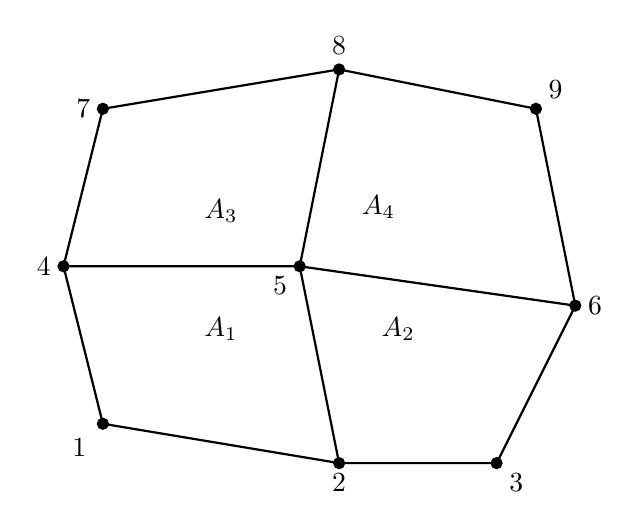
\begin{tikzpicture}
%\draw[fill=gray!5,gray!5](0,0) rectangle (9,7);
%\draw[step=0.5cm,gray,very thin] (0,0) grid (9,7); %background grid
\draw[thick](1.5,1.5) -- (4.5,1) -- (6.5,1) -- (7.5,3) -- (7,5.5) -- (4.5,6) --(1.5,5.5) -- (1,3.5) -- cycle;  
\draw[thick](4.5,1)--(4,3.5)--(4.5,6);
\draw[thick](1,3.5)--(4,3.5)--(7.5,3);
\draw[black,fill=black] (1.5,1.5) circle (2pt); \node[] at (1.2,1.2){1}; %1
\draw[black,fill=black] (4.5,1)   circle (2pt); \node[] at (4.5,0.75){2}; %2
\draw[black,fill=black] (6.5,1)   circle (2pt); \node[] at (6.75,0.75){3}; %3
\draw[black,fill=black] (1,3.5)   circle (2pt); \node[] at (0.75,3.5){4}; %4
\draw[black,fill=black] (4,3.5)   circle (2pt); \node[] at (3.75,3.25){5}; %5
\draw[black,fill=black] (7.5,3)   circle (2pt); \node[] at (7.75,3){6}; %6
\draw[black,fill=black] (1.5,5.5) circle (2pt); \node[] at (1.25,5.5){7}; %7
\draw[black,fill=black] (4.5,6)   circle (2pt); \node[] at (4.5,6.3){8}; %8
\draw[black,fill=black] (7,5.5)   circle (2pt); \node[] at (7.25,5.75){9}; %9
%\draw[thin,dashed](1,3.5)--(4.5,1)--(7.5,3)--(4.5,6)--cycle;
\node[] at (3,2.7){$A_1$}; %8
\node[] at (5.25,2.7){$A_2$}; %8
\node[] at (5,4.25){$A_4$}; %8
\node[] at (3,4.2){$A_3$}; %8
\end{tikzpicture}
\end{center}
\[
q_5^{(1)} = \frac{1}{4}\sum_{e=1}^4 p_e
\] 

In the codes which rely on the $Q_1 \times P_0$ element, the (elemental) pressure
is simply defined as 
\begin{lstlisting}
p=np.zeros(nel,dtype=np.float64)  
\end{lstlisting}
while the nodal pressure is then defined as\footnote{In virtually all stones $p$
stands for the 'raw' pressure and $q$ stands for its projection onto the velocity mesh.} 
\begin{lstlisting}
q=np.zeros(nnp,dtype=np.float64)  
\end{lstlisting}
The element-to-node algorithm is then simply (in 2D):

\begin{lstlisting}
count=np.zeros(nnp,dtype=np.int32)  
for iel in range(0,nel):
    q[icon[0,iel]]+=p[iel]
    q[icon[1,iel]]+=p[iel]
    q[icon[2,iel]]+=p[iel]
    q[icon[3,iel]]+=p[iel]
    count[icon[0,iel]]+=1
    count[icon[1,iel]]+=1
    count[icon[2,iel]]+=1
    count[icon[3,iel]]+=1
q=q/count
\end{lstlisting}

%----------------------------------------------------------------------
\subsection{Schemes 2,3}

{\sl Schemes 2,3} are very similar and are presented in \textcite{sagl81a,sagl81b} (1981).
Scheme 2 uses the areas of the surrounding elements as weights for the arithmetic averaging
while scheme 3 uses the area of the triangles:

\begin{multicols}{2}

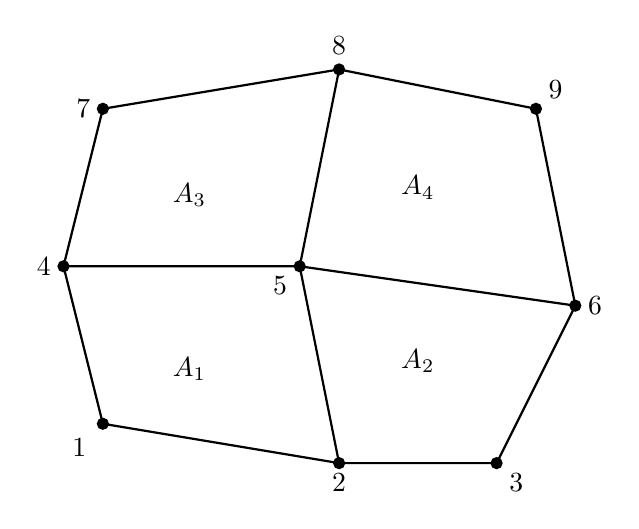
\begin{tikzpicture}
%\draw[fill=gray!5,gray!5](0,0) rectangle (9,7);
%\draw[step=0.5cm,gray,very thin] (0,0) grid (9,7); %background grid
\draw[thick](1.5,1.5) -- (4.5,1) -- (6.5,1) -- (7.5,3) -- (7,5.5) -- (4.5,6) --(1.5,5.5) -- (1,3.5) -- cycle;  
\draw[thick](4.5,1)--(4,3.5)--(4.5,6);
\draw[thick](1,3.5)--(4,3.5)--(7.5,3);
\draw[black,fill=black] (1.5,1.5) circle (2pt); \node[] at (1.2,1.2){1}; %1
\draw[black,fill=black] (4.5,1)   circle (2pt); \node[] at (4.5,0.75){2}; %2
\draw[black,fill=black] (6.5,1)   circle (2pt); \node[] at (6.75,0.75){3}; %3
\draw[black,fill=black] (1,3.5)   circle (2pt); \node[] at (0.75,3.5){4}; %4
\draw[black,fill=black] (4,3.5)   circle (2pt); \node[] at (3.75,3.25){5}; %5
\draw[black,fill=black] (7.5,3)   circle (2pt); \node[] at (7.75,3){6}; %6
\draw[black,fill=black] (1.5,5.5) circle (2pt); \node[] at (1.25,5.5){7}; %7
\draw[black,fill=black] (4.5,6)   circle (2pt); \node[] at (4.5,6.3){8}; %8
\draw[black,fill=black] (7,5.5)   circle (2pt); \node[] at (7.25,5.75){9}; %9
\node[] at (2.6,2.2){$A_1$}; %8
\node[] at (5.5,2.3){$A_2$}; %8
\node[] at (2.6,4.4){$A_3$}; %8
\node[] at (5.5,4.5){$A_4$}; %8
\end{tikzpicture}

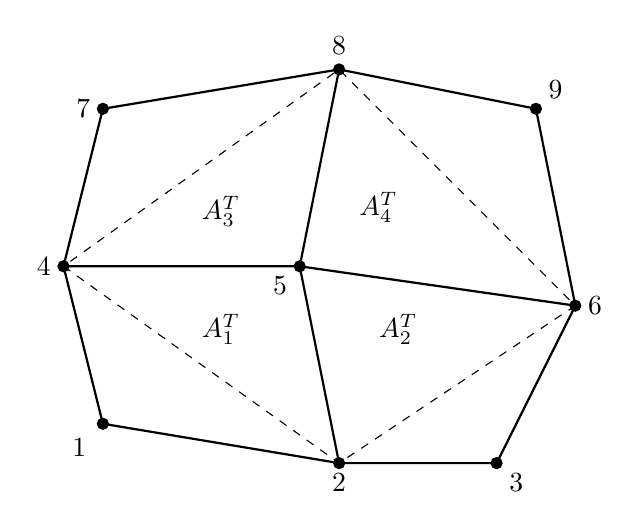
\begin{tikzpicture}
%\draw[fill=gray!5,gray!5](0,0) rectangle (9,7);
%\draw[step=0.5cm,gray,very thin] (0,0) grid (9,7); %background grid
\draw[thick](1.5,1.5) -- (4.5,1) -- (6.5,1) -- (7.5,3) -- (7,5.5) -- (4.5,6) --(1.5,5.5) -- (1,3.5) -- cycle;  
\draw[thick](4.5,1)--(4,3.5)--(4.5,6);
\draw[thick](1,3.5)--(4,3.5)--(7.5,3);
\draw[black,fill=black] (1.5,1.5) circle (2pt); \node[] at (1.2,1.2){1}; %1
\draw[black,fill=black] (4.5,1)   circle (2pt); \node[] at (4.5,0.75){2}; %2
\draw[black,fill=black] (6.5,1)   circle (2pt); \node[] at (6.75,0.75){3}; %3
\draw[black,fill=black] (1,3.5)   circle (2pt); \node[] at (0.75,3.5){4}; %4
\draw[black,fill=black] (4,3.5)   circle (2pt); \node[] at (3.75,3.25){5}; %5
\draw[black,fill=black] (7.5,3)   circle (2pt); \node[] at (7.75,3){6}; %6
\draw[black,fill=black] (1.5,5.5) circle (2pt); \node[] at (1.25,5.5){7}; %7
\draw[black,fill=black] (4.5,6)   circle (2pt); \node[] at (4.5,6.3){8}; %8
\draw[black,fill=black] (7,5.5)   circle (2pt); \node[] at (7.25,5.75){9}; %9
\draw[thin,dashed](1,3.5)--(4.5,1)--(7.5,3)--(4.5,6)--cycle;
\node[] at (3,2.7){$A_1^T$}; %8
\node[] at (5.25,2.7){$A_2^T$}; %8
\node[] at (5,4.25){$A_4^T$}; %8
\node[] at (3,4.2){$A_3^T$}; %8
\end{tikzpicture}

\end{multicols}

\[
q_5^{(2)} = \frac{\sum\limits_{e=1}^4 A_e p_e}{\sum\limits_{e=1}^4 A_e}
\qquad
\qquad
q_5^{(3)} = \frac{\sum\limits_{e=1}^4 A_e^T p_e}{\sum\limits_{e=1}^4 A_e^T}
\] 


\begin{remark} Although Schemes 1,2,3 are similar, scheme 1 is the simplest and fastest
to implement since the areas of neighbouring elements/triangles are not needed.
\end{remark}

\begin{remark} 
Schemes 1,2,3 are identical if all elements are rectangles of identical dimensions.
\end{remark}


%----------------------------------------------------------------------
\subsection{Scheme 4} 

This scheme has been designed by me. 
It resembles the last three ones, but the weighing is in this case different.

Let us consider a 1D problem:
\begin{center}
\includegraphics[width=0.5\linewidth]{images/pressure_smoothing/newalgo.png}
\end{center}

Elemental pressures $p_1$ and $p_2$ corresponding to elements 1 and 2 respectively are known at
locations $x_1$ and $x_2$. The two elements have a different size, characterised in this case
by the distances $d_1$ and $d_2$ to their common edge.

The equation of the line passing through points $(x_1,p_1)$ and $(x_2,p_2)$ is 
\[
p(x)=\frac{p_2-p_1}{x_2-x_1}(x-x_1)+p_1
\]
The $x$ coordinate of the common edge is given by $x=x_1+d_1/2$, 
and since $x_2-x_1=(d_1+d_2)/2$, the 
pressure at this location writes:
\[
p(x_M)= \frac{p_2-p_1}{d_1+d_2}d_1+p_1 = \frac{\frac{p_1}{d_1} + \frac{p_2}{d_2}}{\frac{1}{d_1} + \frac{1}{d_2}}
\]
Extrapolating this formula to 2D, $d_1$ and $d_2$ are in fact the element volumes, so that
\[
q_5^{(4)} = 
\frac{\sum\limits_{j=1}^4 \frac{p_j^e}{A_j^e}}{\sum\limits_{j=1}^4 \frac{1}{A_j^e}}
=
\frac{
\frac{p_1^e}{A_1^e}+
\frac{p_2^e}{A_2^e}+
\frac{p_3^e}{A_3^e}+
\frac{p_4^e}{A_4^e}
}{
\frac{1}{A_1^e}+
\frac{1}{A_2^e}+
\frac{1}{A_3^e}+
\frac{1}{A_4^e}
}\]

There remains a problem, due to the presence of the boundary nodes for which 
the sums present in the above equation do not run up to 4. A boundary
node only has three neighbours and a corner node only two. Additional measures
are required for these nodes. 

\begin{center}
\includegraphics[width=0.5\linewidth]{images/pressure_smoothing/newalgo_corner.png}
\end{center}

The pressure value $p_N$ is obtained as follows:
\[
q_N = \frac{ 
 \frac{p_2^e}   {A_2^e}
+\frac{p_3^e}   {A_3^e}
+\frac{p_{2'}^e}{A_{2'}^e}
+\frac{p_{3'}^e}{A_{3'}^e}
}{
 \frac{1}{A_2^e}
+\frac{1}{A_3^e}
+\frac{1}{A_{2'}^e}
+\frac{1}{A_{3'}^e}
}
\]
The areas and pressures of the mirrored elements 2' and 3' are extrapolated from the areas of elements 2 and 6, and 3 and 7 respectively. 
Likewise the pressure $p_M$ at the corner node is obtained through the pressures of its surrounding elements.


%------------------------------------------------------------------------------
\subsection{Scheme 5 - Least squares} 

This scheme is presented (among other places) in Lee \etal (1979)
\cite{legs79}. 
Let us start from the patch of 4 $Q_1$ elements counting 9 nodes: 

\begin{center}
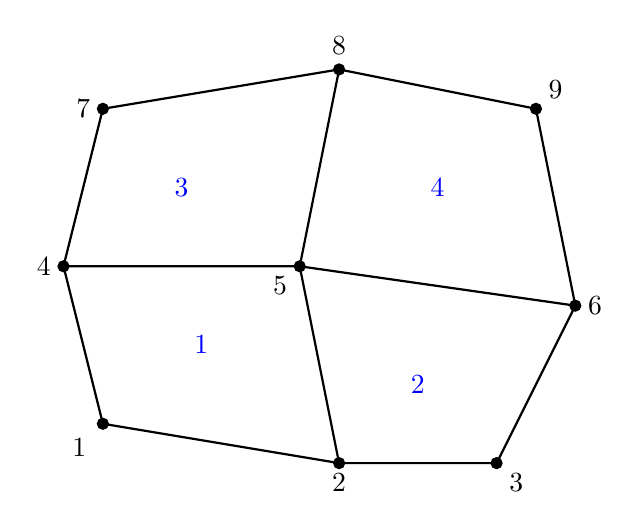
\begin{tikzpicture}
%\draw[fill=gray!5,gray!5](0,0) rectangle (9,7);
%\draw[step=0.5cm,gray,very thin] (0,0) grid (9,7); %background grid
\draw[thick](1.5,1.5) -- (4.5,1) -- (6.5,1) -- (7.5,3) -- (7,5.5) -- (4.5,6) --(1.5,5.5) -- (1,3.5) -- cycle;  
\draw[thick](4.5,1)--(4,3.5)--(4.5,6);
\draw[thick](1,3.5)--(4,3.5)--(7.5,3);

\node[] at (2.75,2.5) {\color{blue}1};
\node[] at (5.5,2) {\color{blue}2};
\node[] at (2.5,4.5) {\color{blue}3};
\node[] at (5.75,4.5) {\color{blue}4};

\draw[black,fill=black] (1.5,1.5) circle (2pt); \node[] at (1.2,1.2){1}; %1
\draw[black,fill=black] (4.5,1)   circle (2pt); \node[] at (4.5,0.75){2}; %2
\draw[black,fill=black] (6.5,1)   circle (2pt); \node[] at (6.75,0.75){3}; %3
\draw[black,fill=black] (1,3.5)   circle (2pt); \node[] at (0.75,3.5){4}; %4
\draw[black,fill=black] (4,3.5)   circle (2pt); \node[] at (3.75,3.25){5}; %5
\draw[black,fill=black] (7.5,3)   circle (2pt); \node[] at (7.75,3){6}; %6
\draw[black,fill=black] (1.5,5.5) circle (2pt); \node[] at (1.25,5.5){7}; %7
\draw[black,fill=black] (4.5,6)   circle (2pt); \node[] at (4.5,6.3){8}; %8
\draw[black,fill=black] (7,5.5)   circle (2pt); \node[] at (7.25,5.75){9}; %9

\end{tikzpicture}
\end{center}



We are looking for a field $q$ living on the nodes.
We build the quantity
\[
J=\iint_\Omega (q-p)^2 dV
\]
where $p$ is the elemental field. To make things clearer we split the integral into 
the sum of elemental integrals:
\[
J=
\iint_{\Omega_1} (q(x,y)-p_1)^2 dV+
\iint_{\Omega_2} (q(x,y)-p_2)^2 dV+
\iint_{\Omega_3} (q(x,y)-p_3)^2 dV+
\iint_{\Omega_4} (q(x,y)-p_4)^2 dV
\]
Inside each element the field $q(x,y)$ is given by a bilinear interpolation so that:
\begin{eqnarray}
J
&=& \iint_{\Omega_1} (\bN_1(x,y) q_1 + \bN_2(x,y)q_2 + \bN_5(x,y)q_5 + \bN_4(x,y)q_4 -p_1)^2 dV \nn\\
&+& \iint_{\Omega_2} (\bN_2(x,y) q_2 + \bN_3(x,y)q_3 + \bN_6(x,y)q_6 + \bN_5(x,y)q_5 -p_2)^2 dV \nn\\
&+& \iint_{\Omega_3} (\bN_4(x,y) q_4 + \bN_5(x,y)q_5 + \bN_8(x,y)q_8 + \bN_7(x,y)q_7 -p_3)^2 dV \nn\\
&+& \iint_{\Omega_4} (\bN_5(x,y) q_5 + \bN_6(x,y)q_6 + \bN_9(x,y)q_9 + \bN_8(x,y)q_8 -p_4)^2 dV 
\end{eqnarray}
where the $N_i$ functions are the basis functions (unusually expressed in $x,y$ coordinates).
The least square procedure looks for the set of $q_i$ such that 
\[
\frac{\partial J}{\partial q_i} =0 \qquad \forall i=1,...9
\]
and this yields 9 equations/constraints for 9 unknowns.
\begin{eqnarray}
\frac{\partial J}{\partial q_1} 
&=& \iint_{\Omega_1} 2 (\bN_1(x,y) q_1 + \bN_2(x,y)q_2 + \bN_5(x,y)q_5 + \bN_4(x,y)q_4 -p_1) \bN_1(x,y) dV \nn\\
\frac{\partial J}{\partial q_2}
&=& \iint_{\Omega_1} 2(\bN_1(x,y) q_1 + \bN_2(x,y)q_2 + \bN_5(x,y)q_5 + \bN_4(x,y)q_4 -p_1) \bN_2(x,y) dV \nn\\
&+& \iint_{\Omega_2} 2(\bN_2(x,y) q_2 + \bN_3(x,y)q_3 + \bN_6(x,y)q_6 + \bN_5(x,y)q_5 -p_2) \bN_2(x,y) dV \nn\\
\frac{\partial J}{\partial q_3}
&=& \iint_{\Omega_2} 2(\bN_2(x,y) q_2 + \bN_3(x,y)q_3 + \bN_6(x,y)q_6 + \bN_5(x,y)q_5 -p_2) \bN_3(x,y) dV \nn\\
\frac{\partial J}{\partial q_4}
&=& \iint_{\Omega_1} 2(\bN_1(x,y) q_1 + \bN_2(x,y)q_2 + \bN_5(x,y)q_5 + \bN_4(x,y)q_4 -p_1) \bN_4(x,y) dV \nn\\
&+& \iint_{\Omega_3} 2(\bN_4(x,y) q_4 + \bN_5(x,y)q_5 + \bN_8(x,y)q_8 + \bN_7(x,y)q_7 -p_3) \bN_4(x,y) dV \nn\\
\frac{\partial J}{\partial q_5}
&=& \iint_{\Omega_1} 2(\bN_1(x,y) q_1 + \bN_2(x,y)q_2 + \bN_5(x,y)q_5 + \bN_4(x,y)q_4 -p_1) \bN_5(x,y) dV \nn\\
&+& \iint_{\Omega_2} 2(\bN_2(x,y) q_2 + \bN_3(x,y)q_3 + \bN_6(x,y)q_6 + \bN_5(x,y)q_5 -p_2) \bN_5(x,y) dV \nn\\
&+& \iint_{\Omega_3} 2(\bN_4(x,y) q_4 + \bN_5(x,y)q_5 + \bN_8(x,y)q_8 + \bN_7(x,y)q_7 -p_3) \bN_5(x,y) dV \nn\\
&+& \iint_{\Omega_4} 2(\bN_5(x,y) q_5 + \bN_6(x,y)q_6 + \bN_9(x,y)q_9 + \bN_8(x,y)q_8 -p_4) \bN_5(x,y) dV \nn\\
\frac{\partial J}{\partial q_6}
&=& \iint_{\Omega_2} 2(\bN_2(x,y) q_2 + \bN_3(x,y)q_3 + \bN_6(x,y)q_6 + \bN_5(x,y)q_5 -p_2) \bN_6(x,y) dV \nn\\
&+& \iint_{\Omega_4} 2(\bN_5(x,y) q_5 + \bN_6(x,y)q_6 + \bN_9(x,y)q_9 + \bN_8(x,y)q_8 -p_4) \bN_6(x,y) dV \nn\\
\frac{\partial J}{\partial q_7}
&=& \iint_{\Omega_3} 2(\bN_4(x,y) q_4 + \bN_5(x,y)q_5 + \bN_8(x,y)q_8 + \bN_7(x,y)q_7 -p_3) \bN_7(x,y) dV \nn\\
\frac{\partial J}{\partial q_8}
&=& \iint_{\Omega_3} 2(\bN_4(x,y) q_4 + \bN_5(x,y)q_5 + \bN_8(x,y)q_8 + \bN_7(x,y)q_7 -p_3) \bN_8(x,y)dV \nn\\
&+& \iint_{\Omega_4} 2(\bN_5(x,y) q_5 + \bN_6(x,y)q_6 + \bN_9(x,y)q_9 + \bN_8(x,y)q_8 -p_4) \bN_8(x,y)dV \nn\\ 
\frac{\partial J}{\partial q_9}
&=& \iint_{\Omega_4} 2(\bN_5(x,y) q_5 + \bN_6(x,y)q_6 + \bN_9(x,y)q_9 + \bN_8(x,y)q_8 -p_4) \bN_9(x,y)dV 
\end{eqnarray}
The factor 2 are removed and the terms $\int p_i N_j $ are known so they end up in the right hand side.
\begin{eqnarray}
 \iint_{\Omega_1} (\bN_1 \bN_1 q_1 + \bN_1 \bN_2 q_2 + \bN_1 \bN_5 q_5 + \bN_1 \bN_4 q_4) dV 
&=& \iint_{\Omega_1} p_1 N_1 dV \nn\\
 \iint_{\Omega_1} (\bN_2 \bN_1 q_1 + \bN_2 \bN_2 q_2 + \bN_2 \bN_5 q_5 + \bN_2 \bN_4 q_4) dV \nn\\
+\iint_{\Omega_2} (\bN_2 \bN_2 q_2 + \bN_3 \bN_2 q_3 + \bN_6 \bN_2 q_6 + \bN_5 \bN_2 q_5) dV 
&=& \iint_{\Omega_1} p_1N_2 dV + \iint_{\Omega_2}  p_2 \bN_2 dV \nn\\
\nn\\
\dots &=& \dots \nn\\
\nn\\
 \iint_{\Omega_4} (\bN_9\bN_5 q_5 + \bN_9\bN_6q_6 + \bN_9\bN_9q_9 + \bN_9\bN_8q_8) dV &=&  \iint_{\Omega_4} p_4 \bN_9 dV 
\end{eqnarray}

The mass matrices corresponding to the four elements are 
\[
{\bm M}_1 = \int_{\Omega_1} \left( \begin{array}{cccc}
 \bN_1 \bN_1 & \bN_1 \bN_2 & \bN_1 \bN_5 & \bN_1 \bN_4 \\
 \bN_2 \bN_1 & \bN_2 \bN_2 & \bN_2 \bN_5 & \bN_2 \bN_4 \\
 \bN_5 \bN_1 & \bN_5 \bN_2 & \bN_5 \bN_5 & \bN_5 \bN_4 \\
 \bN_4 \bN_1 & \bN_4 \bN_2 & \bN_4 \bN_5 & \bN_4 \bN_4 
\end{array}\right) dV
\qquad
{\bm M}_2 = \int_{\Omega_2} \left( \begin{array}{cccc}
 \bN_2 \bN_2 & \bN_2 \bN_3 & \bN_2 \bN_6 & \bN_2 \bN_5 \\
 \bN_3 \bN_2 & \bN_3 \bN_3 & \bN_3 \bN_6 & \bN_3 \bN_5 \\
 \bN_6 \bN_2 & \bN_6 \bN_3 & \bN_6 \bN_6 & \bN_6 \bN_5 \\
 \bN_5 \bN_2 & \bN_5 \bN_3 & \bN_5 \bN_6 & \bN_5 \bN_5 
\end{array}\right) dV
\]
\[
{\bm M}_3 = \int_{\Omega_3} \left( \begin{array}{cccc}
 \bN_4 \bN_4 & \bN_4 \bN_5 & \bN_4 \bN_8 & \bN_4 \bN_7 \\
 \bN_5 \bN_4 & \bN_5 \bN_5 & \bN_5 \bN_8 & \bN_5 \bN_7 \\
 \bN_8 \bN_4 & \bN_8 \bN_5 & \bN_8 \bN_8 & \bN_8 \bN_7 \\
 \bN_7 \bN_4 & \bN_7 \bN_5 & \bN_7 \bN_8 & \bN_7 \bN_7 
\end{array}\right) dV
\qquad
{\bm M}_4 = \int_{\Omega_4} \left( \begin{array}{cccc}
 \bN_5 \bN_5 & \bN_5 \bN_6 & \bN_5 \bN_9 & \bN_5 \bN_8 \\
 \bN_6 \bN_5 & \bN_6 \bN_6 & \bN_6 \bN_9 & \bN_6 \bN_8 \\
 \bN_9 \bN_5 & \bN_9 \bN_6 & \bN_9 \bN_9 & \bN_9 \bN_8 \\
 \bN_8 \bN_5 & \bN_8 \bN_6 & \bN_8 \bN_9 & \bN_8 \bN_8 
\end{array}\right) dV
\]
so that the 9 equations above are actually the result of the assembly process of these four 
elemental systems:
\[
\left( \iint_{\Omega_e} \vec{\bN}^T\vec{\bN} dV \right) \cdot \vec{q}_e = \iint_{\Omega_i} \vec{\bN}^T p_e dV 
\qquad\qquad e=1,2,3,4
\]

Also check section 4.5.4 of \textcite{glte87} (1987), in which the authors 
present a two-step algorithm: 1) pressure is averaged over each element.
2) the nodal values of the pressure are recovered through a least-squares approach.


%------------------------------------------------------------------------------
\subsection{Scheme 6 - Consistent pressure recovery (penalty formulation) \label{ss:cpr}}

This is the method presented in \textcite{zina82} (1982). In the second part 
of this publication the authors wish to establish a simple and effective 
numerical method to calculate variables eliminated by the penalisation process. 
The method involves an additional finite element solution for the nodal 
pressures using the same finite element basis and numerical quadrature 
as used for the velocity.

Let us start with\footnote{I here voluntarily use $q$ instead of $p$}:
\[
q = -\lambda \vec\nabla\cdot \vec\upnu
\]
We are going to treat this equation like any other PDE in the context 
of the FE method, i.e. we are going to establish its weak form. 
We assume that the pressure is given inside an element by
\[
q(x,y) = \sum_{i=1}^{m_\upnu} \bN_i(x,y) q_i = \vec{\bN} \cdot \vec{q}
\]
and the velocity:
\[
\vec\upnu = (u,v) 
\qquad 
\qquad 
u(x,y)  = \sum_{i=1}^{m_\upnu} \bN_i(x,y) u_i
\qquad 
\qquad 
v(x,y)  = \sum_{i=1}^{m_\upnu} \bN_i(x,y) v_i
\]
where the $\bN_i$ are the $Q_1$ basis functions and $q_i$ are the sought after nodal values. 
We multiply the equation above by a $Q_1$ basis function $\bN_i$ and integrate over the whole domain:
\[
\iint_\Omega \bN_i(x,y) q(x,y) \; dxdy 
= -\lambda \iint_\Omega \bN_i \vec\nabla\cdot \vec\upnu  \; dx dy
\]
As before we now focus on the above expression inside a single element $e$:
\[
\iint_{\Omega_e} \bN_i(x,y) q(x,y) \; dxdy = -\lambda \iint_{\Omega_e} \bN_i \vec\nabla\cdot \vec\upnu \; dx dy
\]
After $\bN_i \rightarrow \vec{\bN}=(\bN_1,\bN_2,\bN_3,\bN_4)^T$, the left hand side term becomes:
\[
\iint _{\Omega_e} \vec{\bN}^T q(x,y) \; dxdy 
=
\iint _{\Omega_e} \vec{\bN}^T \vec{\bN} \cdot \vec{q} \; dxdy 
=
\left(\underbrace{\iint _{\Omega_e} \vec{\bN}^T \vec{\bN} dxdy}_{{\bm M}_e} \right) \cdot \vec{q}  
\]
where ${\bm M}_e$ is the elemental mass matrix.
We now turn to the right hand side. We have
\[
\vec\nabla\cdot \vec\upnu
= \frac{\partial u}{\partial x}+\frac{\partial v}{\partial y}
= \sum_i \frac{\partial \bN_i}{\partial x} u_i + \sum_i \frac{\partial \bN_i}{\partial y} v_i 
\]
We here too define $\vec{V}_e=(u_1,v_1,u_2,v_2,u_3,v_3,u_4,v_4)^T$ so that 

\begin{eqnarray}
&& \iint_{\Omega_e} \vec{\bN} {\vec \nabla}\cdot {\vec \upnu} \; dV \nn\\
&=& \iint_{\Omega_e} \vec{\bN}^T \sum_{i=1}^{m_\upnu} 
\left( \frac{\partial \bN_i}{\partial x} u_i + \frac{\partial \bN_i}{\partial y} v_i 
\right)  
dV \label{eq:psmoth6}\\
&=& 
\iint_{\Omega_e} 
\left(
\begin{array}{c}
\bN_1 \left(
\sum\limits_{i=1}^{4} \frac{\partial \bN_i}{\partial x} u_i +
\sum\limits_{i=1}^{4} \frac{\partial \bN_i}{\partial y} v_i \right) \\
\bN_2 \left(
\sum\limits_{i=1}^{4} \frac{\partial \bN_i}{\partial x} u_i +
\sum\limits_{i=1}^{4} \frac{\partial \bN_i}{\partial y} v_i \right) \\
\bN_3 \left(
\sum\limits_{i=1}^{4} \frac{\partial \bN_i}{\partial x} u_i +
\sum\limits_{i=1}^{4} \frac{\partial \bN_i}{\partial y} v_i \right) \\
\bN_4 \left(
\sum\limits_{i=1}^{4} \frac{\partial \bN_i}{\partial x} u_i +
\sum\limits_{i=1}^{4} \frac{\partial \bN_i}{\partial y} v_i \right) 
\end{array}
\right) dV \nonumber \\  %%%%%%%%%%%%%%%%%%%%%%%%%%
&=& 
\int_{\Omega_e} 
\left(
\begin{array}{ccc}
{\bN}_1& {\bN}_1 &  0 \\\\
{\bN}_2& {\bN}_2 &  0 \\\\
{\bN}_3& {\bN}_3 &  0 \\\\
{\bN}_4& {\bN}_4 &  0 
\end{array}
\right)
\cdot
\left(
\begin{array}{c}
\sum\limits_i \frac{\partial \bN_i}{\partial x} u_i \\ \\
\sum\limits_i \frac{\partial \bN_i}{\partial y} v_i \\ \\
\sum\limits_i (\frac{\partial \bN_i}{\partial y} u_i\! +\! \frac{\partial \bN_i}{\partial x} v_i) 
\end{array}
\right)
\; dV \nonumber\\ %%%%%%%%%%%%%%%%%%%%%%%%%%
&=& 
\int_{\Omega_e} 
\underbrace{
\left(
\begin{array}{cccccc}
{\bN}_1 & {\bN}_1 &  0 \\
{\bN}_2 & {\bN}_2 &  0 \\
{\bN}_3 & {\bN}_3 &  0 \\
{\bN}_4 & {\bN}_4 &  0 
\end{array}
\right)
}_{{\bm N}}
\cdot
\underbrace{
\left(\begin{array}{cccccccc}
\partial_x \bN_1 & 0 &  
\partial_x \bN_2 & 0 &  
\partial_x \bN_3 & 0 &  
\partial_x \bN_4 & 0 \\ \\
0 & \partial_y \bN_1 &   
0 & \partial_y \bN_2 &   
0 & \partial_y \bN_3 &   
0 & \partial_y \bN_4 \\ \\
\partial_y \bN_1 & \partial_x \bN_1 &  
\partial_y \bN_2 & \partial_x \bN_2 &  
\partial_y \bN_3 & \partial_x \bN_3 &  
\partial_y \bN_4 & \partial_x \bN_4 
\end{array}\right)}_{{\bm B}}
\cdot \vec{V}_e
\; dV  \nonumber \\
&=& 
\left(\int_{\Omega_e} {\bm N} \cdot {\bm B} \; dV \right) \cdot \vec{V}_e \nonumber\\
&=& -\G_e^T \cdot {\vec V}_e
\end{eqnarray}
This makes sense since $\G^T$ is the discrete divergence operator. However, it is not very efficient to 
build $\G_e$ only to multiply it with a vector of already known quantities. 
In practice we implement Eq.~\eqref{eq:psmoth6} which implmentation resembles the buoyancy term of the 
Stokes equation.

After assembly we arrive at
\[
{\bm M} \cdot \vec{q} = \lambda \G^T \cdot {\vec V} 
\qquad
\text{with}
\qquad
\G_e = -\int_{\Omega_e} {\bm N} \cdot {\bm B} \; dV
\]
where ${\bm M}$ is the global mass matrix, $\vec{q}$ the vector of all 
nodal pressures, $\G$ the discrete gradient matrix and $\vec{V}$
the (velocity) solution vector. 
The system can be easily solved since the mass matrix is a friendly matrix.
The vector ${\vec q}$ contains the nodal pressure values directly, with 
no need for a smoothing scheme! 

\begin{remark}
Very importantly, the mass matrix ${\bm M}$ is to be evaluated at the full integration points, 
while the constraint part (the right hand side of the equation) is to be evaluated at 
the reduced integration point, i.e. in the middle of the element.  
\end{remark}

\begin{remark}
As noted in \cite{zina82}, it is interesting to note that when linear elements are used 
and the lumped matrices are used for the ${\bm M}$ the resulting algebraic equation is identical 
to the smoothing scheme 1 only if a uniform square finite element 
mesh is used. In this respect this method is expected to yield different results when elements 
are not square or even rectangular.
\end{remark}

\begin{remark}
The third column of the matrix ${\bm N}$
and the last line of the ${\bm B}$ matrix could be removed altogether.
If your code is based on the mixed formulation, then you already 
have built matrix $\G$ so you can easily re-use this piece of code 
to compute $\G$ again, this time with a reduced integration quadrature.
If you are using the penalty formulation then you need to program 
all from scratch and then simply do away with these unnecessary terms, or 
you can direcly build the rhs as $\int_{\Omega_e} \vec{\bN}^T p_e$ (assuming
you have previously computed the pressure in the middle of each element 
by means of $p=-\lambda\vec\nabla\cdot\vec\upnu$).
\end{remark}

\begin{remark}
This  scheme is identical to the least square scheme!
\end{remark}


%--------------------------------------------------------------
\subsection{Scheme 7}

Same as scheme 6, but with lumped mass matrix.  


%--------------------------------------------------------------
\subsection{Scheme 8 - bilinear interpolation} 

Let us assume that the centers of the 
four elements make a $Q_1$ quadrilateral element, as shown on this figure:

\input{tikz/tikz_pscheme8}

The values at the corners are $p_1$,
$p_2$, $p_3$ and $p_4$. Assuming that the pressure inside this element 
can be represented by a bilinear field, we have 
\[
p(x,y)= a+ bx +cy +dxy
\]
where the coefficients will be determined by ensuring that 
$p(x_i,y_i)=p_i$ for $i=1,2,3,4$, or:
\begin{eqnarray}
a+bx_1+cy_1+dx_1y_1 &=& p_1 \\
a+bx_2+cy_2+dx_2y_2 &=& p_2 \\
a+bx_3+cy_3+dx_3y_3 &=& p_3 \\
a+bx_4+cy_4+dx_4y_4 &=& p_4 
\end{eqnarray}
i.e.
\[
\left(
\begin{array}{cccc}
1 & x_1 & y_1 & x_1y_1 \\
1 & x_2 & y_2 & x_2y_2 \\
1 & x_3 & y_3 & x_3y_3 \\
1 & x_4 & y_4 & x_4y_4
\end{array}
\right)\cdot
\left(
\begin{array}{c}
a \\b\\c\\d
\end{array}
\right)
=
\left(
\begin{array}{c}
p_1\\p_2\\p_3\\p_4
\end{array}
\right)
\]

There remains an issue with nodes which are on the boundaries of the 
domain. These are of course not 'surrounded' by four pressure values 
so the above algorithm does not apply directly. However, looking 
at the above figure, and assuming that node 1 is a lower left corner 
of a 2D domain, we can use the bilinear interpolation based on elements 
1,2,3,4 to extrapolate a nodal pressure value at node 1. 
The same would apply for nodes 2 and 4 for example. 

\begin{remark}
This scheme is not applicable to quadtree-based meshed.
\end{remark}





\newpage %-----------------------------------------------------------------------------------------
\newpage %-----------------------------------------------------------------------------------------
\section{The value of the timestep}\label{ss:cfl} \input{cfl} %------------------------------------
\newpage %-----------------------------------------------------------------------------------------
\section{Mappings \& Jacobians \label{ss:mappings}} \begin{flushright} {\tiny {\color{gray} mappings.tex}} \end{flushright}
%~~~~~~~~~~~~~~~~~~~~~~~~~~~~~~~~~~~~~~~~~~~~~~~~~~~~~~~~~~~~~~~~~~~~~~~~~~~~~~~~~~~~~~~~~~~~~~~~~~

\index{general}{Isoparametric}
\index{general}{Subparametric} 
\index{general}{Superparametric}

The name {\sl isoparametric} derives from the fact that the same ('iso') 
functions are used as basis functions and for the mapping to the reference element.

More generally, if $n_e$ denotes the number of nodes of an element and $n_g$ denotes the 
number of nodes describing the geometry of the element, 
then the element is termed {\sl subparametric} when $n_g<n_e$ and 
{\sl superparametric} when $n_g>n_e$.

%...........................................
\subsubsection{Linear mapping on a triangle}

\begin{verbatim}
2
|\     s
| \    |_r
|  \
3===1
\end{verbatim}

Let us assume that the coordinates of the vertices are 
$(x_1,y_1)$,  
$(x_2,y_2)$, and 
$(x_3,y_3)$.
The coordinates inside the reference element are $(r,s)$ with 
$0\le r \le 1$ and $0 \le s \le 1$. We then simply have the 
following relationship, i.e. any point of the reference element 
can be mapped to the physical triangle as follows:
\begin{eqnarray}
x&=& r x_1 + s x_2 + (1-r-s) x_3 \\
y&=& r y_1 + s y_2 + (1-r-s) y_3 
\end{eqnarray} 
Note that the functions $r$, $s$ and $1-r-s$ are in fact the 
$P_1$ basis functions (see Section~\ref{ss:p1}).
There is also an inverse map, which is easily computed:
\begin{eqnarray}
r&=& \frac{(y_2-y_3)(x-x_3)-(x_2-x_3)(y-y_3)}{(x_1-x_3)(y_2-y_3)-(y_1-y_3)(x_2-x_3)} \\
s&=& \frac{-(y_1-y_3)(x-x_3)+(x_1-x_3)(y-y_3)}{(x_1-x_3)(y_2-y_3)-(y_1-y_3)(x_2-x_3)} 
\end{eqnarray} 
\begin{remark}
The denominator will not vanish, because it is a multiple of the area of the 
triangle. If the three points
are distinct then the area cannot be zero.
\end{remark}

%................................................
\subsubsection{Bilinear mapping on a quadrilateral}

The \index{general}{reference element} reference element 
is in the $(r,s)$ space. It is a square of size $2\times2$ 
centered around the origin, i.e. $(r,s)\in[-1,1]\times[-1,1]$. 
We wish to map it to the quadrilateral in the $(x,y)$ space 
(and vice versa):

\begin{center}
\includegraphics[width=8cm]{images/mappings/bilinear/mapping_bilinear.png}
\end{center}

The coordinates of the vertices are 
$(x_1,y_1)$, $(x_2,y_2)$, $(x_3,y_3)$ and $(x_4,y_4)$.
We then simply have the 
following relationship, i.e. any point of the reference element 
can be mapped to the physical quadrilateral as follows:
\begin{eqnarray}
x&=& \bN_1(r,s) x_1 + \bN_2(r,s) x_2 + \bN_3(r,s) x_3 + \bN_4(r,s) x_4 \\
y&=& \bN_1(r,s) y_1 + \bN_2(r,s) y_2 + \bN_3(r,s) y_3 + \bN_4(r,s) y_4 
\end{eqnarray} 
where the $Q_1$ basis functions $\bN_i(r,s)$ are defined in Section~\ref{sec:elts1D}.

In the following example the program randomly generates 10000 points 
inside the reference 
element and computes their mapping into the $(x,y)$ space. 

\begin{lstlisting}
x1=-1 ; y1=-2
x2=3  ; y2=-1
x3=2  ; y3=2
x4=-3 ; y4=1

npts=10000
r=np.zeros(npts,dtype=np.float64)   
s=np.zeros(npts,dtype=np.float64)   
x=np.zeros(npts,dtype=np.float64)   
y=np.zeros(npts,dtype=np.float64)   

for i in range(0,npts):
    # compute random r,s coordinates
    r[i]=random.uniform(-1.,+1)
    s[i]=random.uniform(-1.,+1)
    # compute basis function values at r,s
    N1=0.25*(1-r[i])*(1-s[i])
    N2=0.25*(1+r[i])*(1-s[i])
    N3=0.25*(1+r[i])*(1+s[i])
    N4=0.25*(1-r[i])*(1+s[i])
    # compute x,y coordinates
    x[i]=N1*x1+N2*x2+N3*x3+N4*x4
    y[i]=N1*y1+N2*y2+N3*y3+N4*y4

np.savetxt('rs.ascii',np.array([r,s]).T)
np.savetxt('xy.ascii',np.array([x,y]).T)
\end{lstlisting}

\begin{center}
\includegraphics[width=7cm]{images/mappings/bilinear/rs.pdf}
\includegraphics[width=7cm]{images/mappings/bilinear/xy.pdf}
\end{center}

There is also an inverse map, which is not so easily computed (see Section~\ref{sec:amiin}).
However, if the quadrilateral in the $(x,y)$ space is a rectangle of size $(h_x,h_y)$, 
the inverse mapping is trivial:
\begin{eqnarray}
r&=&\frac{x-x_1}{x_2-x_1} \\
s&=&\frac{y-y_1}{y_4-y_1} 
\end{eqnarray}
Also in the case of rectangular elements of size $(h_x,h_y)$
the basis functions can easily be written as functions of $(x,y)$:
\begin{eqnarray}
\bN_1(x,y) &=& \left( \frac{x_3 -x }{h_x}  \right) \left( \frac{y_3 -y }{h_y}  \right) \nn\\
\bN_2(x,y) &=& \left( \frac{x - x_1}{h_x}  \right) \left( \frac{y_3 -y }{h_y}  \right) \nn\\
\bN_3(x,y) &=& \left( \frac{x - x_1}{h_x}  \right) \left( \frac{y - y_1}{h_y}  \right) \nn\\
\bN_4(x,y) &=& \left( \frac{x_3 -x }{h_x}  \right) \left( \frac{y - y_1}{h_y}  \right) \nn 
\end{eqnarray}
On the one hand, any variable defined on the element can be approximated using the basis functions:
\begin{equation}
f^h(r,s)=\sum_i \bN_i(r,s) f_i.
\end{equation}
If we treat the coordinate variables $x$ and $y$ themselves as functions, 
then the basis functions can be used to construct the mapping:
\begin{equation}
x(r,s)=\sum_i \bN_i(r,s) x_i 
\qquad
y(r,s)=\sum_i \bN_i(r,s) y_i,  \label{eqxy}
\end{equation}
leading to write
\begin{eqnarray}
\frac{\partial x}{\partial r} &=& \sum_i \frac{\partial \bN_i}{\partial r} x_i \\
\frac{\partial x}{\partial s} &=& \sum_i \frac{\partial \bN_i}{\partial s} x_i \\
\frac{\partial y}{\partial r} &=& \sum_i \frac{\partial \bN_i}{\partial r} y_i \\
\frac{\partial y}{\partial s} &=& \sum_i \frac{\partial \bN_i}{\partial s} y_i 
\end{eqnarray}
On the other hand we also have 
\begin{eqnarray}
\frac{\partial f}{\partial r} &=&
\frac{\partial f}{\partial x}\frac{\partial x}{\partial r}
+\frac{\partial f}{\partial y}\frac{\partial y}{\partial r} \\
\frac{\partial f}{\partial s} &=&
\frac{\partial f}{\partial x}\frac{\partial x}{\partial s}
+\frac{\partial f}{\partial y}\frac{\partial y}{\partial s}
\end{eqnarray}
or in matrix form:
\begin{equation}
\left(
\begin{array}{c}
\frac{\partial f}{\partial r} \\ \\
\frac{\partial f}{\partial s}
\end{array}
\right)
=
\underbrace{
\left(
\begin{array}{cc}
\frac{\partial x}{\partial r} & \frac{\partial y}{\partial r} \nonumber\\ \\
\frac{\partial x}{\partial s} & \frac{\partial y}{\partial s} \nonumber
\end{array}
\right)
}_{\bm J}
\cdot
\left(
\begin{array}{c}
\frac{\partial f}{\partial x} \\ \\
\frac{\partial f}{\partial y}
\end{array}
\right)
\end{equation}
where ${\bm J}$ is called the Jacobian of the transformation
By inverting the Jacobian matrix, the desired derivatives with respect to $x$
and $y$ can be obtained:

We have:
\[
\left(
\begin{array}{c}
\frac{\partial f}{\partial x} \\ \\
\frac{\partial f}{\partial y}
\end{array}
\right)
=
{\bm J}^{-1} \cdot 
\left(
\begin{array}{c}
\frac{\partial f}{\partial r} \\ \\
\frac{\partial f}{\partial s}
\end{array}
\right)
\]
The inverse of the Jacobian matrix can be simply obtained in 
2D (Cramer's rule for $2\times2$ matrices\footnote{\url{https://en.wikipedia.org/wiki/Cramers_rule}}):
\[
{\bm J}^{-1} = \frac{1}{|{\bm J}|} 
\left(
\begin{array}{cc}
\frac{\partial y}{\partial s} & -\frac{\partial y}{\partial r} \nonumber\\ \\
-\frac{\partial x}{\partial s} & \frac{\partial x}{\partial r} \nonumber
\end{array}
\right)
\]
The presence of the determinant in the denominator implies that it cannot 
be zero anywhere, or in other words: the mapping is not valid if $|{\bm J}|$
is zero anywhere over the element.

\begin{remark}
\textcite{hua90} (1990) has published analytical inverse transformation 
for quadrilateral isoparametric elements, i.e. how to compute ${\bm J}^{-1}$ 
as a function of space coordinates and not just at the quadrature points. 
\end{remark}

Let us look at this by means of a simple example and let us consider the following 
element:
\begin{center}
\includegraphics[width=4cm]{images/mappings/fournode/ex1}
\end{center}
Then a $Q_1$ mapping yields:
\begin{eqnarray}
x(r,s) &=& \sum_i \bN_i(r,s) x_i = \bN_2 + 2\bN_3 = \frac{1}{4} (3+3r+ s+rt) \nn\\
y(r,s) &=& \sum_i \bN_i(r,s) y_i = 2\bN_3 + \bN_4 = \frac{1}{4} (3+r+ 3s+rt) 
\end{eqnarray}
The Jacobian matrix is then
\begin{equation}
{\bm J} = 
\left(
\begin{array}{cc}
\frac{\partial x}{\partial r} & \frac{\partial y}{\partial r} \nonumber\\ \\
\frac{\partial x}{\partial s} & \frac{\partial y}{\partial s} \nonumber
\end{array}
\right)
=
\frac{1}{4}
\left(
\begin{array}{cc}
3+s & 1+s \\
1+r & 3+r
\end{array}
\right)
\end{equation}
and its determinant is 
\begin{equation}
|{\bm J}|=\frac{1}{4} [(3+s)(3+r)-(1+s)(1+r)]=\frac{1}{2}+\frac{1}{8}r+\frac{1}{8}s
\end{equation}
It is clear that $|{\bm J}|>0$ for $-1\leq r \leq +1$ and $-1\leq s \leq +1$. 

Let us now consider another example, the following element:
\begin{center}
\includegraphics[width=3.5cm]{images/mappings/fournode/ex2}
\end{center}
It follows that
\begin{eqnarray}
x(r,s) &=& \sum_i \bN_i(r,s) x_i = \frac{1}{4}(1+r)(7+5s) \\ 
y(r,s) &=& \sum_i \bN_i(r,s) y_i = \frac{1}{4}(17+5r+7s-5rs)
\end{eqnarray}
and the determinant:
\[
|{\bm J}|=\frac{3}{2}-\frac{15r}{4}+\frac{15s}{4}
\]
is zero for $r-s=2/5$. This mapping is invalid!

\begin{remark}
Problems also arise when the Jacobian matrix is nearly singular due to round-off errors.
To avoid problems linked to badly shaped elements, it is recommended that the inside
angles of an element are larger than $15\degree$ and less than $165\degree$.
\end{remark}

From Eq.~\eqref{eqxy}, we can also write:
\begin{eqnarray}
dx &=& \frac{\partial x}{\partial r} dr + \frac{\partial x}{\partial s} ds \\
dy &=& \frac{\partial y}{\partial r} dr + \frac{\partial y}{\partial s} ds 
\end{eqnarray}
or, 
\begin{equation}
\left(
\begin{array}{c}
dx \\ dy
\end{array}
\right)
={\bm J}\cdot
\left(
\begin{array}{c}
dr \\ ds
\end{array}
\right)
\end{equation}
This means that integrating over the 'real' element in $(x,y)$ space
can be simply done by integrating of the reference element in the 
$(r,s)$ space. This is the cornerstone of most of the implementation of the 
Finite Element Method, the second integral being carried out by means 
of the Gauss-Legendre quadrature.

\begin{equation}
\iint_{\Omega_e} ... \; dx dy = \int_{-1}^{+1} \int_{-1}^{+1} ...|{\bm J}| \; dr ds
\end{equation}


%.................................................................
\subsubsection{Biquadratic mapping of a straight-edge face $Q_2$ element }

\begin{center}
\includegraphics[width=8cm]{images/mappings/biquadratic/mapping1}
\end{center}

The reference element now contains 9 nodes: 1,3,7,9 are the corners, nodes
2,4,6,8 are the mid-face points and node 5 is in the middle\footnote{Note that 
this numbering is quite arbitrary}.
The mapping from the $(r,s)$ space to the $(x,y)$ space is then as follows:

\begin{eqnarray}
\left(
\begin{array}{c}
x(r,s) \\ y(r,s)
\end{array}
\right)
&=&
\bN_1(r,s)
\left(
\begin{array}{c}
x_1 \\ y_1
\end{array}
\right)
+
\bN_2(r,s)
\left(
\begin{array}{c}
x_2 \\ y_2
\end{array}
\right)
+
\bN_3(r,s)
\left(
\begin{array}{c}
x_3 \\ y_3
\end{array}
\right)
+
\bN_4(r,s)
\left(
\begin{array}{c}
x_4 \\ y_4
\end{array}
\right) \nonumber\\
&+&
\bN_5(r,s)
\left(
\begin{array}{c}
x_5 \\ y_5
\end{array}
\right)
+
\bN_6(r,s)
\left(
\begin{array}{c}
x_6 \\ y_6
\end{array}
\right)
+
\bN_7(r,s)
\left(
\begin{array}{c}
x_7 \\ y_7
\end{array}
\right)
+
\bN_8(r,s)
\left(
\begin{array}{c}
x_4 \\ y_8
\end{array}
\right) \nonumber\\
&+&
\bN_9(r,s)
\left(
\begin{array}{c}
x_9 \\ y_9
\end{array}
\right) 
\nonumber
\end{eqnarray}
where the $Q_2$ basis functions have been obtained in Section~\ref{ss:q22d}:
\begin{eqnarray}
\bN_1(r,t)&=& 0.5r(r-1)  0.5t(t-1) \nonumber\\
\bN_2(r,t)&=&      (1-r^2)  0.5t(t-1) \nonumber\\
\bN_3(r,t)&=& 0.5r(r+1)  0.5t(t-1) \nonumber\\
\bN_4(r,t)&=& 0.5r(r-1)       (1-t^2) \nonumber\\
\bN_5(r,t)&=&      (1-r^2)       (1-t^2) \nonumber\\
\bN_6(r,t)&=& 0.5r(r+1)       (1-t^2) \nonumber\\
\bN_7(r,t)&=& 0.5r(r-1)  0.5t(t+1) \nonumber\\
\bN_8(r,t)&=&      (1-r^2)  0.5t(t+1) \nonumber\\
\bN_9(r,t)&=& 0.5r(r+1)  0.5t(t+1) \nonumber
\end{eqnarray}


\begin{lstlisting}
x1=-1                 ; y1=-2
x3=3                  ; y3=-1
x9=2                  ; y9=2
x7=-3                 ; y7=1
x2=0.5*(x1+x3)        ; y2=0.5*(y1+y3)
x4=0.5*(x1+x7)        ; y4=0.5*(y1+y7)
x6=0.5*(x3+x9)        ; y6=0.5*(y3+y9)
x8=0.5*(x7+x9)        ; y8=0.5*(y7+y9)
x5=0.25*(x1+x3+x7+x9) ; y5=0.25*(y1+y3+y7+y9)

npts=10000
r=np.zeros(npts,dtype=np.float64)   
s=np.zeros(npts,dtype=np.float64)   
xQ1=np.zeros(npts,dtype=np.float64)   
yQ1=np.zeros(npts,dtype=np.float64)   
xQ2=np.zeros(npts,dtype=np.float64)   
yQ2=np.zeros(npts,dtype=np.float64)   

for i in range(0,npts):
    # compute random r,s coordinates
    r[i]=random.uniform(-1.,+1)
    s[i]=random.uniform(-1.,+1)
    # compute Q2 basis function values at r,s
    N1= 0.5*r[i]*(r[i]-1.) * 0.5*s[i]*(s[i]-1.)
    N2=       (1.-r[i]**2) * 0.5*s[i]*(s[i]-1.)
    N3= 0.5*r[i]*(r[i]+1.) * 0.5*s[i]*(s[i]-1.)
    N4= 0.5*r[i]*(r[i]-1.) *       (1.-s[i]**2)
    N5=       (1.-r[i]**2) *       (1.-s[i]**2)
    N6= 0.5*r[i]*(r[i]+1.) *       (1.-s[i]**2)
    N7= 0.5*r[i]*(r[i]-1.) * 0.5*s[i]*(s[i]+1.)
    N8=       (1.-r[i]**2) * 0.5*s[i]*(s[i]+1.)
    N9= 0.5*r[i]*(r[i]+1.) * 0.5*s[i]*(s[i]+1.)
    # compute x,y coordinates
    xQ2[i]=N1*x1+N2*x2+N3*x3+N4*x4+N5*x5+N6*x6+N7*x7+N8*x8+N9*x9
    yQ2[i]=N1*y1+N2*y2+N3*y3+N4*y4+N5*y5+N6*y6+N7*y7+N8*y8+N9*y9
    # compute Q1 basis function values at r,s
    N1=0.25*(1-r[i])*(1-s[i])
    N2=0.25*(1+r[i])*(1-s[i])
    N3=0.25*(1+r[i])*(1+s[i])
    N4=0.25*(1-r[i])*(1+s[i])
    # compute x,y coordinates
    xQ1[i]=N1*x1+N2*x3+N3*x9+N4*x7
    yQ1[i]=N1*y1+N2*y3+N3*y9+N4*y7

np.savetxt('rs.ascii',np.array([r,s]).T)
np.savetxt('xyQ1.ascii',np.array([xQ1,yQ1]).T)
np.savetxt('xyQ2.ascii',np.array([xQ2,yQ2]).T)
\end{lstlisting}

The code is available in {\tt /images/mappings/biquadratic}
Note that the coordinates of point 5 are defined being those of the barycenter
of the quadrilateral. More on this choice later.

\begin{center}
a)\includegraphics[width=5.6cm]{images/mappings/biquadratic/rs.pdf}
b)\includegraphics[width=5.6cm]{images/mappings/biquadratic/xyQ1.pdf}
c)\includegraphics[width=5.6cm]{images/mappings/biquadratic/xyQ2.pdf}\\
{\captionfont a) 10,000 random points in the reference element; 
b,c) image of these points by means of a bilinear and biquadratic mapping 
respectively.\\ When the sides of the element
are straight we see that a $Q_1$ mapping is sufficient.}
\end{center}

%.................................................................
\subsubsection{Biquadratic mapping of a not-so straight-line face $Q_2$ element }

We now carry out the same exercise as before but nodes 2 and 8 are no more 
in the middle of nodes 1-3 and 7-9 respectively.
The code is available in {\tt /images/mappings/biquadratic2}.

\begin{center}
a)\includegraphics[width=4.5cm]{images/mappings/biquadratic2/rs.pdf}
b)\includegraphics[width=4.5cm]{images/mappings/biquadratic2/xyQ1.pdf}
c)\includegraphics[width=4.5cm]{images/mappings/biquadratic2/xyQ2.pdf}\\
{\captionfont a) 10,000 random points in the reference element; 
b,c) image of these points by means of a bilinear and biquadratic mapping 
respectively.} 
\end{center}

In this case we see that 
the $Q_2$ mapping manages to better capture the 'real' shape of the element.
Since nodes 2 and 8 have moved, we could now ask ourselves 
where we should place node 5? In this example we set it as follows
but it is somewhat arbitrary.
\begin{lstlisting}
x5=(x1+x2+x3+x4+x6+x7+x8+x9)/8. 
y5=(y1+y2+y3+y4+y6+y7+y8+y9)/8.
\end{lstlisting}
We will come back to this later.

%.......................................................................
\subsubsection{Bilinear, biquadratic and bicubic mapping in an annulus }

In the light of what precedes, we can now ask ourselves how this translates to 
a real geodynamic case. Let us then consider the case of an annular domain, 
a cross section of a hollow sphere. 
When using quadrilateral elements, the mesh will look similar to this:

\begin{center}
\includegraphics[width=6cm]{images/mappings/curved/annulus_mesh}
\end{center}

We here focus on $Q_1$, $Q_2$ and $Q_3$ mappings. We single out an element, 
and arbitrarily define it as follows in polar coordinates:
\begin{lstlisting}
theta1=23./180.*np.pi
theta2=52./180.*np.pi
R1=1.
R2=1.5
\end{lstlisting}
The $Q_1$ mapping requires four points, the $Q_2$ nine points and the $Q_3$
sixteen points. 
The code used in the following is available at {\tt ./images/mappings/curved/}.
These are placed equidistantly in the $r,\theta$ coordinate
system, as shown hereunder:

\begin{center}
\includegraphics[width=5.7cm]{images/mappings/curved/nodesQ1.pdf}
\includegraphics[width=5.7cm]{images/mappings/curved/nodesQ2.pdf}
\includegraphics[width=5.7cm]{images/mappings/curved/nodesQ3.pdf}\\
{\captionfont Left to right: position of the nodes for the $Q_1$, $Q_2$ and $Q_3$ mappings.
$Q_4$ is not shown.}
\end{center}

As before, we randomly shoot 10,000 points inside the reference element 
and map these out in the $x,y$ space. Resulting swarms of points are shown 
in the following figures:

\begin{center}
\includegraphics[width=5.7cm]{images/mappings/curved/xy1_keep.pdf}
\includegraphics[width=5.7cm]{images/mappings/curved/xy2_keep.pdf}
\includegraphics[width=5.7cm]{images/mappings/curved/xy3_keep.pdf}\\
{\captionfont Left to right: position of the mapped points for the $Q_1$, $Q_2$ and $Q_3$ mappings.
$Q_4$ is not shown.}
\end{center}

The image of a square with a $Q_1$ mapping is obviously a quadrilateral
so that it looks like quite a few points land outside of the domain $R_1\leq r\leq R_2$.
Note that points are well within $23\degree \leq \theta \leq 52\degree$, which can 
simply be explained by the fact that the faces of the element joining $R_1$
to $R_2$ are straight lines.

However, it looks like the biquadratic and bicubic mappings are doing a much better 
job at mapping the region of space $R_1\leq r\leq R_2$. In order to characterise 
this better, we now place 10,000 points on the bottom face of 
the reference element (i.e. $s=-1$)
and once again compute their coordinates in the the $x,y$ space:

\begin{center}
\includegraphics[width=8cm]{images/mappings/curved/xy1.pdf}
\includegraphics[width=8cm]{images/mappings/curved/xy2.pdf}\\
\includegraphics[width=8cm]{images/mappings/curved/xy3.pdf}
\includegraphics[width=8cm]{images/mappings/curved/xy4.pdf}\\
{\captionfont Position of the mapped points for the $Q_1$, $Q_2$, $Q_3$ and $Q_4$ mappings.}
\end{center}

For each point $i$ we now compute the distance $r_i$ 
to the origin, which, if the 
mapping was perfect, would be exactly equal to $R_1=1$. 
On the following plots are shown the error $r_i-1$ for all 
points, from $r=-1$ to $r=+1$.

\begin{center}
\includegraphics[width=8cm]{images/mappings/curved/innerline_error_Q1mapping.pdf}
\includegraphics[width=8cm]{images/mappings/curved/innerline_error_Q2mapping.pdf}\\
\includegraphics[width=8cm]{images/mappings/curved/innerline_error_Q3mapping.pdf}
\includegraphics[width=8cm]{images/mappings/curved/innerline_error_Q4mapping.pdf}\\
{\captionfont Radius error of the mapped points for the $Q_1$, $Q_2$, $Q_3$ and $Q_4$ mappings.}
\end{center}

We see that the amplitude of the error decreases with the order of the mapping used, 
which is why for instance \aspect uses a $Q_4$ mapping by default\footnote{I find it also quite striking 
that the $Q_4$ mapping outperforms the $Q_3$ one by two orders of magnitude...}.
Actually, in this particular case, the equation which describes the circle is not a 
polynomial so that no high-order mapping will ever be able to {\it exactly} 
represent the curved boundary of the element!

Another interesting point to keep in mind is that the location of the quadrature points
in the $x,y$ space is also determined by the mapping used, which can have consequences
on the accuracy of the integration and it will be reflected (for instance) on the 
error convergence rate.

As already mentioned previously, 
the coordinates of the nodes of the element in the $x,y$ are 
uniquely determined when they are on the convex hull of the element (
for instance nodes 0-7 for $Q_2$) but we need to choose the position 
of the last nodes which are inside the element. Unfortunately, this choice is 
not neutral. 

Finally, we can explore the importance of the mapping in combination with 
numerical quadrature. For each mapping we compute the area of the element
by means of a 3x3, 4x4 or 5x5 quadrature.

\begin{verbatim}
**********Q1*********
nqperdim= 3 0.3030060126539606 rel. error -0.04215361698430029
nqperdim= 4 0.3030060126539606 rel. error -0.04215361698430012 ~ 4%
nqperdim= 5 0.3030060126539606 rel. error -0.04215361698430012
**********Q2*********
nqperdim= 3 0.3162980025394154 rel. error -0.00013569026611326453
nqperdim= 4 0.3162980025394155 rel. error -0.00013569026611308905 ~ 0.01%
nqperdim= 5 0.3162980025394154 rel. error -0.00013569026611326453
**********Q3*********
nqperdim= 3 0.3163472223929359 rel. error 1.9900899402587318e-05
nqperdim= 4 0.316347222392936  rel. error 1.9900899402938278e-05 ~ 0.002%
nqperdim= 5 0.316347222392936  rel. error 1.9900899402938278e-05
**********Q4*********
nqperdim= 3 0.3163409410866220 rel. error 4.477021014282521e-08
nqperdim= 4 0.3163409541901677 rel. error 8.619243716974044e-08 ~ 0.000008%
nqperdim= 5 0.316340954190168  rel. error 8.619243804713484e-08
\end{verbatim}

Here again the $Q_4$ mapping makes quite the difference. 

\newpage

%..................................................................
\subsubsection{Biquadratic mapping - the middle node conundrum}

Python code at {\tt images/mappings/biquadratic3}.

As mentioned before, unless the element is a straight-edge quadrilateral, 
determining the (best) position of the middle node is not trivial. Or is it?


\begin{verbatim}

4--7--3
|     |
8  9  6   (reference element)
|     |
1--5--2

\end{verbatim}

We will here consider 5 different elements:

\begin{center}
\includegraphics[width=3.5cm]{images/mappings/biquadratic3/elt0/element0}
\includegraphics[width=3.5cm]{images/mappings/biquadratic3/elt1/element1}
\includegraphics[width=3.5cm]{images/mappings/biquadratic3/elt2/element2}
\includegraphics[width=3.5cm]{images/mappings/biquadratic3/elt3/element3}
\includegraphics[width=3.5cm]{images/mappings/biquadratic3/elt4/element4}\\
{\captionfont From left to right: element 0,1,2,3,4.}
\end{center}

We can think of multiple ways to come up with the 'center' of the element, 
i.e. the location of point I.

\begin{itemize}
\item {\python center=0}: 
\[
x_9=(x_1+x_2+x_3+x_4)/4 
\qquad
y_9=(y_1+y_2+y_3+y_4)/4
\]

\item {\python center=1}: 
\[
x_9=(x_1+x_2+x_3+x_4+x_5+x_6+x_7+x_8)/8 
\qquad
y_9=(y_1+y_2+y_3+y_4+y_5+y_6+y_7+y_8)/8
\]
\item {\python center=2}:
\[
x_9=(x_1+x_2+x_3+x_4+3x_5+3x_6+3x_7+3x_8)/16. 
\qquad
y_9=(y_1+y_2+y_3+y_4+3y_5+3y_6+3y_7+3y_8)/16.
\]
\item {\python center=3}: (only element=4)
\[
x_9=\frac12(R_1+R_2)\cos(3\pi/8) 
\qquad
y_9=\frac12(R_1+R_2)\sin(3\pi/8)
\]
\item {\python center=4}: I is the center of mass. 
The element is defined by $R_1<r<R_2$ and $\theta_1<\theta<\theta_2$.

We need to compute\footnote{\url{https://en.wikipedia.org/wiki/Center_of_mass}}
\begin{eqnarray}
\vec{R} 
&=&\frac{1}{M} \int \vec{r} \rho(\vec r) dV \nn\\
&=&\frac{1}{M} \rho_0 \int \vec{r} dV\nn\\
&=&\frac{1}{M} \frac{M}{V} \int \vec{r} dV\nn\\
&=&\frac{1}{V} \int \vec{r} dV\nn\\
&=&\frac{1}{V} \int \left(\begin{array}{c} x \\ y \end{array}\right)  dV\nn\\
&=&\frac{1}{V} \int \left(\begin{array}{c} r \cos \theta \\ r \sin\theta \end{array}\right)dV\nn\\
&=&\frac{1}{V} \int_{R_1}^{R_2} \int_{\theta_1}^{\theta_2} \left(\begin{array}{c} r \cos \theta 
\\ r \sin\theta \end{array}\right)  r dr d\theta\nn\\
&=&\frac{1}{\frac12 (R_2^2-R_1^2) (\theta_2-\theta_1)} \frac13(R_2^3-R_1^3) 
\left(
\begin{array}{c}
\sin\theta_2-\sin\theta_1 \\
-\cos\theta_2+\cos\theta_1 
\end{array}
\right) \nn\\
&\simeq& 
\left(
\begin{array}{c}
0.5801028000103104\\
1.4004920473554983
\end{array}
\right) 
\end{eqnarray}
which corresponds to $r=1.5158816686291174$ and $\theta=67.5^o=3\pi/8$.

\item {\python center=5}: variable position
\end{itemize}


isoparametric mapping. 


At each point $(r,s)$ we compute the error $|\sum_i N_i(r,s) x_i^2 - (\sum_i N_i(r,s) x_i)^2|$.

position of edges (setting r=+- 1, s=+-1) independent of position of middle node since shape functions are zero there

area indep of position middle node ?



%....................
\paragraph{Element 0}

In this case all only {\python center=0,1,2,4} are applicable but they all 
lead to the same point I with $x_I=0,y_I=0$. This means that the position of 
quadrature points is also independent of the {\python center} parameter.
 
\begin{center}
\includegraphics[width=5.7cm]{images/mappings/biquadratic3/elt0/jcob}
\includegraphics[width=5.7cm]{images/mappings/biquadratic3/elt0/error_posx2}
\includegraphics[width=5.7cm]{images/mappings/biquadratic3/elt0/error_posy2}\\
{\captionfont 10,000 points at random.} 
\end{center}

%....................
\paragraph{Element 1}

In this case all only {\python center=0,1,2,4} are applicable but they all 
lead to the same point I with $x_I=0,y_I=0$. This means that the position of 
quadrature points is also independent of the {\python center} parameter.
 
\begin{center}
\includegraphics[width=5.7cm]{images/mappings/biquadratic3/elt1/jcob}
\includegraphics[width=5.7cm]{images/mappings/biquadratic3/elt1/error_posx2}
\includegraphics[width=5.7cm]{images/mappings/biquadratic3/elt1/error_posy2}\\
{\captionfont 10,000 points at random.} 
\end{center}


%....................
\paragraph{Element 2} .

\begin{center}
\includegraphics[width=5.7cm]{images/mappings/biquadratic3/elt2/jcob_0}
\includegraphics[width=5.7cm]{images/mappings/biquadratic3/elt2/jcob_1}
\includegraphics[width=5.7cm]{images/mappings/biquadratic3/elt2/jcob_2}\\
\includegraphics[width=5.7cm]{images/mappings/biquadratic3/elt2/error_posx2_0}
\includegraphics[width=5.7cm]{images/mappings/biquadratic3/elt2/error_posx2_1}
\includegraphics[width=5.7cm]{images/mappings/biquadratic3/elt2/error_posx2_2}\\
\includegraphics[width=5.7cm]{images/mappings/biquadratic3/elt2/error_posy2_0}
\includegraphics[width=5.7cm]{images/mappings/biquadratic3/elt2/error_posy2_1}
\includegraphics[width=5.7cm]{images/mappings/biquadratic3/elt2/error_posy2_2}\\
{\captionfont 50,000 points at random. From left to right: center=0,1,2.} 
\end{center}




%....................
\paragraph{Element 3} .

\begin{center}
\includegraphics[width=5.7cm]{images/mappings/biquadratic3/elt3/jcob_0}
\includegraphics[width=5.7cm]{images/mappings/biquadratic3/elt3/jcob_1}
\includegraphics[width=5.7cm]{images/mappings/biquadratic3/elt3/jcob_2}\\
{\captionfont 50,000 points at random. From left to right: center=0,1,2.} 
\end{center}




%....................
\paragraph{Element 4}


\begin{center}
\includegraphics[width=5.7cm]{images/mappings/biquadratic3/elt4/jcob_0}
\includegraphics[width=5.7cm]{images/mappings/biquadratic3/elt4/jcob_1}
\includegraphics[width=5.7cm]{images/mappings/biquadratic3/elt4/jcob_2}\\
\includegraphics[width=5.7cm]{images/mappings/biquadratic3/elt4/jcob_3}
\includegraphics[width=5.7cm]{images/mappings/biquadratic3/elt4/jcob_4}\\
{\captionfont 50,000 points at random. From left to right: center=0,1,2,3,4.} 
\end{center}




\begin{center}
\includegraphics[width=8.5cm]{images/mappings/biquadratic3/elt4/nodes}
\includegraphics[width=8.5cm]{images/mappings/biquadratic3/elt4/quads}\\
{\captionfont Left: position of the nodes. Right position of quadrature points with 
nqperdim=3.}
\end{center}

\begin{verbatim}

\end{verbatim}

Area does not depend on position of middle node?!




\vspace{1cm}

\Literature 
\begin{itemize}
\item \fullcite{yuhy94}
\end{itemize}








 
 %-----------------------------
\newpage %-----------------------------------------------------------------------------------------
\section{Exporting data to vtk/vtu format} 
This format seems to be the universally accepted format for 2D and 3D visualisation in 
Computational Geodynamics (and even CFD ?). Such files can be opened with open source 
softwares such as 
Paraview \footnote{https://www.paraview.org/}, 
MayaVi \footnote{https://docs.enthought.com/mayavi/mayavi/}
or Visit \footnote{https://wci.llnl.gov/simulation/computer-codes/visit/}.

Unfortunately it is my experience that no simple tutorial exists about how to build 
such files. There is an official document which describes the vtk 
format\footnote{https://www.vtk.org/wp-content/uploads/2015/04/file-formats.pdf}
but it delivers the information in a convoluted way. I therefore describe hereafter 
how fieldstone builds the vtk files. 

I hereunder show vtk file corresponding to a 3x2 grid made of linear elements.
In this particular example there are:
\begin{itemize}
\item 12 nodes and 6 elements
\item 1 elemental field (the pressure {\tt p}
\item 2 nodal fields: 1 scalar (the smoothed pressure {\tt q}), 1 vector (the velocity field {\tt u,v,0})
\end{itemize}
Note that vtk files are inherently 3D so that even in the case of a 2D simulation the $z$-coordinate 
of the points and for instance their $z$-velocity component must be provided.
The file, usually called {\filenamefont solution.vtk} starts with a header:

\lstinputlisting[language=python,firstline=1,lastline=3]{images/vtk/solution.vtu}

We then proceed to write the node coordinates as follows:

\lstinputlisting[language=python,firstline=4,lastline=19]{images/vtk/solution.vtu}

These are followed by the elemental field(s):

\lstinputlisting[language=python,firstline=20,lastline=29]{images/vtk/solution.vtu}

Nodal quantities are written next:

\lstinputlisting[language=python,firstline=30,lastline=59]{images/vtk/solution.vtu}

To these informations we must append 3 more datasets. The first one is the connectivity, 
the second one is the offsets and the third one is the type. The first one is trivial
since the required connectivity array is the same as the one needed for the Finite Elements. 
The second must be understood as follows:
when reading the connectivity information in a linear manner the offset values 
indicate the beginning of each element (omitting the zero value). The third is simply the type of element 
as given in the vtk format document (9 corresponds to a generic quadrilateral with an 
internal numbering consistent with ours). 

\lstinputlisting[language=python,firstline=60,lastline=85]{images/vtk/solution.vtu}

The file is then closed with

\lstinputlisting[language=python,firstline=86,lastline=88]{images/vtk/solution.vtu}

The {\sl solution.vtu}\footnote{\url{https://raw.githubusercontent.com/cedrict/fieldstone/master/images/vtk/solution.vtu}}  
can then be opened with ParaView, MayaVi or Visit and the reader 
is advised to find tutorials online on how to install and use these softwares. Also check Appendix~\ref{app:paraview}.

\begin{center}
\includegraphics[width=4cm]{images/vtk/grid}
\includegraphics[width=4cm]{images/vtk/vel}
\includegraphics[width=4cm]{images/vtk/press}
\end{center}

In the same folder {\tt images/vtk} there is the python script 
{\pythonfile makevtu.py}\footnote{\url{https://raw.githubusercontent.com/cedrict/fieldstone/master/images/vtk/makevtu.py}} which produces 3 different vtu files. The first one {\sl solution1.vtu} is a similar to the one above: an \lstinline{nelx*nely} quadrilateral-based mesh in a unit square. 
The second one ({\sl solution2.vtu}) looks identical when opened in Paraview but it is rather different: each element is exported as its own sub-mesh, so that if the mesh counts nel elements the number of vertices is \lstinline{4*nel}, and not \lstinline{(nelx+1)(nely+1)}. As such this file is larger. The icon array is needed to write down the positions of the four vertices of each element but not to write down the connectivity since the first 4 points are making the 1st element, the next four points are making the second element, etc ...

\begin{lstlisting}
vtufile.write("<Points> \n")
vtufile.write("<DataArray type='Float32' NumberOfComponents='3' Format='ascii'> \n")
for iel in range(0,nel):
    if not flag[iel]:
       for k in range(0,m):
           vtufile.write("%10e %10e %10e \n" %(x[icon[k,iel]],y[icon[k,iel]],0.))
vtufile.write("</DataArray>\n")
vtufile.write("</Points> \n")
vtufile.write("<Cells>\n")
vtufile.write("<DataArray type='Int32' Name='connectivity' Format='ascii'> \n")
for iel in range (0,nel_left):
    vtufile.write("%d %d %d %d \n" %(iel*4,iel*4+1,iel*4+2,iel*4+3))
vtufile.write("</DataArray>\n")
...
vtufile.write("</Cells>\n")
\end{lstlisting}

This format is rather practical in the case of linear or higher order discontinuous fields. For example, in the case of the $Q_2\times P_{-1}$ element pair, the pressure is linear inside each element and discontinuous across element edges. One can then assign pressure values at the four vertices of each element.

Finally a third mesh {\sl solution3.vtu} is produced. It is based on the 2nd one, but since elements are now somewhat de-coupled, then one can export only a subset of the mesh. For instance one could not show elements which are two distorted, or below a certain line, or outside a certain volume, etc ... In {\pythonfile makevtu.py} all elements which center is inside a circle are flagged and will not be exported into the vtu file:
\begin{lstlisting}
for iel in range(0,nel):
    flag[iel]= (xc[iel]-0.333*Lx)**2+(yc[iel]-0.666*Ly)**2<0.234**2
nel_flagged=np.sum(flag)
nel_left=nel-nel_flagged
\end{lstlisting}

\begin{center}
\includegraphics[width=11cm]{images/vtk/mesh3}
\end{center}





 %------------------------------
\newpage %-----------------------------------------------------------------------------------------
\section{Runge-Kutta methods}\label{ss:rkm} These methods were developed around 1900 by the German mathematicians Carl Runge and Martin Kutta.
The RK methods are methods for the numerical integration of 
ODEs\footnote{\url{https://en.wikipedia.org/wiki/Runge-Kutta_methods}}. These methods are well 
documented in any numerical analysis textbook and the reader is referred to \cite{gery10,tack10}.
Any Runge-Kutta method is uniquely identified by its Butcher tableau (REF?) which contains 
all necessary coefficients to build the algorithm.\todo{missing refs for Butcher tableau}

You will find here\footnote{\url{https://en.wikipedia.org/wiki/List_of_Runge-Kutta_methods}}
a complete list of RK methods.

The simplest Runge-Kutta method is the (forward) Euler method. Its tableau is:

\begin{mdframed}[backgroundcolor=blue!5]
\begin{tabular}{c|c}
0 & \\
\hline
 & 1
\end{tabular}
\end{mdframed}

\index{general}{Midpoint Method} \index{general}{RK2}
The standard second-order RK method method (also called midpoint method) is:

\begin{mdframed}[backgroundcolor=blue!5]
\begin{tabular}{c|cccccc}
0 & \\
1/2 & 1/2 \\
\hline
 & 0 & 1 
\end{tabular}
\end{mdframed}

\index{general}{Heun's emthod}
Another second-order RK method, called Heun's 
method\footnote{\url{https://en.wikipedia.org/wiki/Heun's_method}} is follows:

\begin{mdframed}[backgroundcolor=blue!5]
\begin{tabular}{c|cccccc}
0 & \\
1 & 1 \\
\hline
 & 1/2 & 1/2 
\end{tabular}
\end{mdframed}

A third-order RK method is as follows:\index{general}{RK3}

\begin{mdframed}[backgroundcolor=blue!5]
\begin{tabular}{c|ccccc}
0 & \\
1/2 & 1/2 \\
1 & -1 & 2 \\ 
\hline
 & 1/6 & 4/6  & 1/6
\end{tabular}
\end{mdframed}


\index{general}{RK4}
The RK4 method falls in this framework. Its tableau is:

\begin{mdframed}[backgroundcolor=blue!5]
\begin{tabular}{c|cccccc}
0 & \\
1/2 & 1/2 \\
1/2 & 0 & 1/2 \\
1 & 0 & 0 & 1 \\
\hline
 & 1/6 & 1/3 & 1/3 & 1/6 
\end{tabular}
\end{mdframed}

A slight variation of the standard RK4 method is also due to Kutta in 1901 and is called the 3/8-rule. 
Almost all of the error coefficients are smaller than in the standard method but it requires 
slightly more FLOPs per time step. Its Butcher tableau is

\begin{mdframed}[backgroundcolor=blue!5]
\begin{tabular}{c|cccccc}
0 & \\
1/3 & 1/3 \\
2/3 & -1/3 & 1 \\
1 & 1 & -1 & 1 \\
\hline
 & 1/8 & 3/8 & 3/8 & 1/8 
\end{tabular}
\end{mdframed}


\index{general}{RK45} \index{general}{Runge-Kutta-Fehlberg method}
The following method is called the Runge-Kutta-Fehlberg method and is 
commonly abbreviated 
RKF45\footnote{\url{https://en.wikipedia.org/wiki/Runge-Kutta-Fehlberg_method}}. 
Its Butcher tableau is as follows: 

\begin{mdframed}[backgroundcolor=blue!5]
\begin{tabular}{c|cccccc}
0 & \\
1/4 	&1/4\\ 
3/8 	&3/32 		&9/32 \\
12/13 	&1932/2197 	&-7200/2197 &	7296/2197\\
1 	&439/216 	&-8 	&3680/513 &	-845/4104\\
1/2 	&-8/27 		&2 	&-3544/2565& 	1859/4104 &	-11/40 	\\
\hline
&16/135 	&0 		&6656/12825 	&28561/56430 	&-9/50& 	2/55\\
&25/216 	&0 	&1408/2565 	&2197/4104 	&-1/5 	&0 
\end{tabular}
\end{mdframed}


The first row of coefficients at the bottom of the table gives the fifth-order 
accurate method, and the second row gives the fourth-order accurate method. 

The particularity of this method is that from the same Butcher Tableau one 
can produce a 4th-order approximation $\tilde{A}$ and a 5th-order approximation $A$:
\begin{eqnarray}
\tilde{A}_{n+1}&=&A_n + \frac{25}{216}A_1 + \frac{1408}{2565}A_3+\frac{2197}{4101}A_4 -\frac15 A_5 \nn\\
A_{n+1}&=&A_n + \frac{16}{135}A_1 + \frac{6656}{12825}A_3+\frac{28561}{56430}A_4 \nn
-\frac{9}{50} A_5 + \frac{2}{55} A_6
\end{eqnarray}
One can define 
\[
R=\frac{1}{h} | \tilde{A}_{n+1} - A_{n+1} | \nn\\
\qquad\qquad
\delta = \left( \frac{tol}{R \sqrt 2} \right)^{1/4}
\]
where $h$ is the current step.
If $R \le tol$ keep $A$ as the current step solution and move to the next step with step size $\delta  \cdot h$.
If $R > tol$ recalculate the current step with step size $\delta  \cdot h$. 



In the literature we can also find even higher order methods 
based on the same principle:

\begin{center}
\includegraphics[width=8cm]{images/rungekutta/fe7}\\
\includegraphics[width=10cm]{images/rungekutta/prdo81a}\\
\includegraphics[width=14cm]{images/rungekutta/prdo81b}\\
{\captionfont Top: 7th order Fehlberg method; 
Middle and bottom: 6/5th and 8/7th order Dormand-Prince methods from \cite{prdo81}.}
\end{center}

\Literature:
\textcite{dopr80} (1980),
\textcite{fehl85} (1985),
\textcite{dopr86} (1986),
\textcite{caka90} (1990),
\textcite{hanw93} (1993),
\textcite{butcher03}.


%....................................................................................
\subsubsection{Using RK methods to advect particles/markers \label{sec:rkparticles}}

In the context of geodynamical modelling, one is usually faced with the following problem:
now that I have a velocity field on my FE (or FD) mesh, how can I use it to advect the Lagrangian 
markers?

Runge-Kutta methods are used to this effect but only their spatial component is used:
the velocity solution is not recomputed at the intermediate fractional timesteps, i.e. 
only the coefficients of the right hand side of the tableaus is used.

\begin{itemize}
\item The RK1 method is simple.

\begin{tabular}{c|c}
0 & \\
\hline
 & 1
\end{tabular}

\noindent Carry out a loop over markers and 
\begin{enumerate}
\item interpolate velocity $\vec\upnu_{m}$ onto each marker $m$
\item compute new position as follows: $\vec r_m(t+\delta t)=\vec r_m(t) + \vec\upnu_m \delta t$
\end{enumerate}

\item The RK2 method is also simple but requires a bit more work.

\begin{tabular}{c|cccccc}
0 & \\
1 & 1 \\
\hline
 & 1/2 & 1/2 
\end{tabular}

\noindent Carry out a loop over markers and 
\begin{enumerate}
\item interpolate velocity $\vec\upnu_{m}$ onto each marker $m$ at position $\vec r_m$
\item compute new intermediate position as follows: $\vec r_m^{(1)}(t+\delta t)=\vec r_m(t) + \vec\upnu_m \delta t/2$
\item compute velocity $\vec\upnu_{m}^{(1)}$ at position $\vec r_m^{(1)}$
\item compute new position: $\vec r_m(t+\delta t)=\vec r_m(t) + \vec\upnu_m^{(1)} \delta t$ 
\end{enumerate}
Note that the intermediate positions could be in a different element of the mesh so extra 
care must be taken when computing intermediate velocities. 

\item 
The RK3 method introduces two intermediate steps. 

\begin{tabular}{c|ccccc}
0 & \\
1/2 & {\color{chestnut} $\frac{1}{2}$ } \\
1 & {\color{violet}-1} & {\color{violet}2} \\ 
\hline
 & {\color{carrotorange} $\frac16$} & {\color{carrotorange} $\frac46$}  & {\color{carrotorange} $\frac16$}
\end{tabular}

Carry out a loop over markers and 
\begin{enumerate}
\item interpolate velocity $\vec\upnu_{m}$ onto each marker $m$ at position $\vec r_m$
\item compute new intermediate position as follows: 
$\vec r_m^{(1)}(t+\delta t)=\vec r_m(t) + {\color{chestnut} \frac{1}{2}} \vec\upnu_m \delta t$
\item compute velocity $\vec\upnu_{m}^{(1)}$ at position $\vec r_m^{(1)}$
\item compute new intermediate position as follows: 
$\vec r_m^{(2)}(t+\delta t)=\vec r_m(t) + ( {\color{violet}-1} \vec\upnu_m 
+ {\color{violet}2} \vec\upnu_m^{(1)} ) \delta t$
\item compute velocity $\vec\upnu_{m}^{(2)}$ at position $\vec r_m^{(2)}$
\item compute new position: 
$\vec r_m(t+\delta t)=\vec r_m(t) + ( 
{\color{carrotorange} \frac16} \vec\upnu_m + 
{\color{carrotorange} \frac46} \vec\upnu_m^{(1)} + 
{\color{carrotorange} \frac16} \vec\upnu_m^{(2)}    )\delta t$ 
\end{enumerate}

\end{itemize}

The following example is borrowed from \cite{maie12}, itself borrowed from Fullsack \cite[Section 5.4]{full95}.
It is a whirl flow \cite{otti89}, a flow with rotational symmetry in which concentric layers of material
rotate around  a centre with an angular velocity:
\[
\omega(r)= \omega_0 \frac{r}{r_0} \exp\left(-\frac{r}{r_0}  \right)
\]  
The box is $[-0.5,0.5]\times[-0.5,0.5]$, $r_0=0.25$, $\omega_0=0.3$ and $\delta t=1$. 
$60\times 60$ particles are regularly positioned inside the $[-0.3,0.3]\times[-0.3,0.3]$ square.
Maierova \cite{maie12} has carried out this experiment for the above Runge-Kutta methods.

\begin{center}
\includegraphics[height=4cm]{images/rk/maie12a}\\
{\captionfont Model domain with particles colored at three
different time-steps: (A) t = 0 (initial position of particles), (B) t = 50, and (C) t = 200.
The advection is computed using the fourth-order Runge-Kutta scheme. Taken from \cite{maie12}}
\end{center}

\begin{center}
\includegraphics[height=4cm]{images/rk/maie12b}
\includegraphics[height=4cm]{images/rk/maie12c}\\
{\captionfont The same plot as above, but for different advection schemes at t = 100.
Advection was computed using (A) the fourth-order Runge-Kutta scheme, (B) the mid-
point method, (C) Heun's method and (D) the explicit Euler method. Taken from \cite{maie12}}
\end{center}


 %-----------------------------------
\newpage %-----------------------------------------------------------------------------------------
\section{Am I in or not? - finding reduced coordinates}\label{sec:amiin}
It is quite common that at some point one must answer the question:
"Given a mesh and its connectivity on the one hand, and the coordinates of a 
point on the other, how do I accurately and quickly determine in which element 
the point resides?"

One typical occurence of such a problem is linked to the use of the Particle-In-Cell 
technique: particles are advected and move through the mesh, and need to be localised 
at every time step. This question could arise in the context of a benchmark where 
certain quantities need to be measured at specific locations inside the domain. 

%-------------------------------------------
%-------------------------------------------
\subsubsection{Two-dimensional space}

We shall first focus on quadrilaterals. There are many kinds of quadrilaterals as shown 
hereunder: 

\begin{center}
\includegraphics[width=12cm]{images/quadrilaterals} \\
{\captionfont Taken from Wikipedia 
\url{https://en.wikipedia.org/wiki/Quadrilateral#/media/File:Quadrilaterals.svg}}
\end{center}

%..................................................
\paragraph{The trivial case of rectangular elements} 

Testing whether the point $M$ is inside the element is trivial. 
For $x_0 \leq x_M \leq x_2$ and $y_0 \leq y_M \leq y_2$, its reduced coordinates
are given by
\begin{eqnarray}
r_M &=& \frac{2}{x_2-x_0}(x_M-x_0) -1 = \frac{2}{h_x}(x_M-x_0)-1  \nn\\
s_M &=& \frac{2}{y_2-y_0}(y_M-y_0) -1 = \frac{2}{h_y}(y_M-y_0)-1  
\end{eqnarray}

\begin{center}
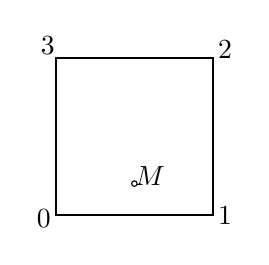
\begin{tikzpicture}
%\draw[step=0.5cm,gray,very thin] (0,0) grid (4,4); %background grid
\draw[thick] (1,1) -- (3,1) -- (3,3) -- (1,3) -- cycle;  
\node[] at (0.85,0.95) {0};
\node[] at (3.15,1) {1};
\node[] at (3.15,3.1) {2};
\node[] at (0.9,3.15) {3};
\node[] at (2.2,1.5) {$M$};
\draw (2.,1.4) circle (1pt);
\end{tikzpicture}\\
\end{center}


%..................................................
\paragraph{An intermediate case} We make the following assumption that the lateral sides of the  
element are vertical while the bottom and top are not necessarily horizontal:

\begin{center}
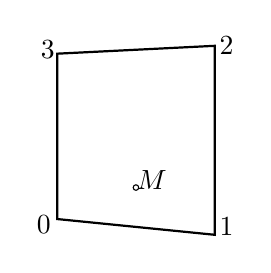
\begin{tikzpicture}
%\draw[step=0.5cm,gray,very thin] (0,0) grid (4,4); %background grid
\draw[thick] (1,1) -- (3,0.8) -- (3,3.2) -- (1,3.1) -- cycle;  
\node[] at (0.83,0.93) {0};
\node[] at (3.15,0.9) {1};
\node[] at (3.15,3.2) {2};
\node[] at (0.88,3.15) {3};
\node[] at (2.2,1.5) {$M$};
\draw (2.,1.4) circle (1pt);
\end{tikzpicture}\\
\end{center}

\noindent Because the sides are verical then if $x_0 \leq x_M \leq x_2$ then 
\[
r_M = \frac{2}{x_2-x_0}(x_M-x_0) -1 
\]
Then, if $M$ is inside the element then its $y$ coordinate is given by
\[
y_M = \sum_i \bN_i(r_M,s_M) y_i
\]
where $\bN_i$ are the four $Q_1$ basis functions associated to the vertices.
Assuming we know $r_M$ then we can solve for $s_M$:
\begin{eqnarray}
y_M &=&  
\frac{1}{4}(1-r_M)(1-s_M) y_0+
\frac{1}{4}(1+r_M)(1-s_M) y_1+
\frac{1}{4}(1+r_M)(1+s_M) y_2+
\frac{1}{4}(1-r_M)(1+s_M) y_3 \nn\\
&=& 
\frac{1}{4} \left[
(1-r)y_0+(1+r)y_1+(1+r)y_2+(1-r)y_3 +s_M [ -(1-r)y_0 - (1+r)y_1+(1+r)y_2+(1-r)y_3  ] 
\right] \nn 
\end{eqnarray}
or, 
\[
s_M = \frac{ 4y_M - [(1-r_M)y_0+(1+r_M)y_1+(1+r_M)y_2+(1-r_M)y_3]  }{ -(1-r_M)y_0 -(1+r_M)y_1+(1+r_M)y_2+(1-r_M)y_3 } 
\]
If the obtained value is in $[-1,1]$ then the point $M$ is in the element.
Verification: when $y_1=y_0$ and $y_2=y_3$ then 
\begin{eqnarray}
s_M 
&=& \frac{4 y_M - [(1-r_M)y_0+(1+r_M)y_0+(1+r_M)y_3+(1-r_M)y_3]  }{ -(1-r_M)y_0 - (1+r_M)y_0+(1+r_M)y_3+(1-r_M)y_3 } \nn\\
&=& \frac{4 y_M - [ 2 y_0 + 2 y_3]  }{ -2 y_0 + 2 y_3    }  \nn\\
&=& \frac{1}{y_3-y_0} [2 y_M - (  y_0 +  y_3) ] \nn\\ 
&=& \frac{1}{y_3-y_0} [2 y_M -  2 y_0 +y_0 -  y_3)  ] \nn\\ 
&=& \frac{2}{y_3-y_0} (y_M - y_0) - 1 
\end{eqnarray}
which is the expression that corresponds to a rectangular element as seen previously.

%..................................................
\paragraph{A generic quadrilateral}

We wish to arrive at a single algorithm which is applicable to all quadrilaterals and we now focus  
on an irregular quadrilateral (no face is parallel to the axis of the coordinate system). 

\begin{center}
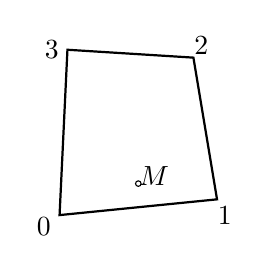
\begin{tikzpicture}
%\draw[step=0.5cm,gray,very thin] (0,0) grid (4,4); %background grid
\draw[thick] (1,1) -- (3,1.2) -- (2.7,3) -- (1.1,3.1) -- cycle;  
\node[] at (0.8,0.85) {0};
\node[] at (3.1,1) {1};
\node[] at (2.8,3.15) {2};
\node[] at (0.9,3.1) {3};
\node[] at (2.2,1.5) {$M$};
\draw (2.,1.4) circle (1pt);
\end{tikzpicture}\\
\end{center}

\noindent Several rather simple options exist:
\begin{itemize}
\item we could subdivide the quadrilateral into two triangles and check whether point $M$ is inside any of them (as it turns out, this problem is rather straightforward for triangles. Simply google it.)
\item We could check that point $M$ is always on the left side of segments $0\rightarrow 1$, $1\rightarrow 2$, $2\rightarrow 3$, $3\rightarrow 0$.
\item ...  
\end{itemize}

Any of these approaches will work although some might be faster than others. 
In three-dimensions all will however become 
cumbersome to implement and might not even work at all. 
Fortunately, there is an elegant way to answer the question, as 
detailed in the following subsection, which works both in 2D and 3D.

%-------------------------------------------
\subsubsection{Three-dimensional space}

If point $M$ is inside the quadrilateral, there exist a set of reduced 
coordinates $r,s,t\in[-1:1]^3$ such that 

\[
\sum_{i=1}^4 \bN_i(r_M,s_M,t_M) x_i = x_M
\quad\quad\quad
\sum_{i=1}^4 \bN_i(r_M,s_M,t_M) y_i = y_M
\quad\quad\quad
\sum_{i=1}^4 \bN_i(r_M,s_M,t_M) z_i = z_M
\]
This can be cast as a system of three equations and three unknowns. 
Unfortunately, each basis function $\bN_i$ 
contains a term $rst$ (as well as $rs$, $rt$, and $st$) 
so that it is not a linear system.
We must then use an iterative technique: the algorithm starts with 
a guess for values $r_M,s_M,t_M$ and 
improves on their value iteration after iteration. 
In what follows the subscript $M$ is dropped from $r,s,t$.

The classical way of solving nonlinear systems of equations is Newton's method. 
\index{general}{Newton's method}
We can rewrite the equations above as ${\bm F}(r,s,t)=0$:
\begin{eqnarray}
\sum_{i=1}^8 \bN_i(r,s,t) x_i - x_M&=&0 \nonumber\\
\sum_{i=1}^8 \bN_i(r,s,t) y_i - y_M&=&0 \nonumber\\
\sum_{i=1}^8 \bN_i(r,s,t) z_i - z_M&=&0
\end{eqnarray}
or,
\begin{eqnarray}
F_r(r,s,t)&=&0 \nonumber\\
F_s(r,s,t)&=&0 \nonumber\\
F_t(r,s,t)&=&0 \nonumber
\end{eqnarray}
so that we now have to find the zeroes of continuously differentiable 
functions ${\bm F}:\mathbb{R} \rightarrow \mathbb{R}$.
The recursion is simply:
\[
\left(
\begin{array}{c}
r_{k+1} \\s_{k+1} \\ t_{k+1}
\end{array}
\right)
=
\left(
\begin{array}{c}
r_{k} \\s_{k} \\ t_{k}
\end{array}
\right)
- J_F(r_k,s_k,t_k) ^{-1} 
\left(
\begin{array}{c}
F_r(r_k,s_k,t_k) \\
F_s(r_k,s_k,t_k)\\
F_t(r_k,s_k,t_k)
\end{array}
\right)
\]
where $J$ the Jacobian matrix:
\begin{eqnarray}
J_F(r_k,s_k,t_k)
&=&
\left(
\begin{array}{ccc}
\frac{\partial F_r}{\partial r}(r_k,s_k,t_k) & \frac{\partial F_r}{\partial s}(r_k,s_k,t_k) & \frac{\partial F_r}{\partial t}(r_k,s_k,t_k) \\\\
\frac{\partial F_s}{\partial r}(r_k,s_k,t_k) & \frac{\partial F_s}{\partial s}(r_k,s_k,t_k) & \frac{\partial F_s}{\partial t}(r_k,s_k,t_k) \\\\
\frac{\partial F_t}{\partial r}(r_k,s_k,t_k) & \frac{\partial F_t}{\partial s}(r_k,s_k,t_k) & \frac{\partial F_t}{\partial t}(r_k,s_k,t_k) 
\end{array}
\right) \nonumber\\
&=&
\left(
\begin{array}{ccc}
\sum\limits_{i=1}^8 \frac{\partial \bN_i}{\partial r}(r_k,s_k,t_k) x_i &
\sum\limits_{i=1}^8 \frac{\partial \bN_i}{\partial s}(r_k,s_k,t_k) x_i &
\sum\limits_{i=1}^8 \frac{\partial \bN_i}{\partial t}(r_k,s_k,t_k) x_i \\
\sum\limits_{i=1}^8 \frac{\partial \bN_i}{\partial r}(r_k,s_k,t_k) y_i &
\sum\limits_{i=1}^8 \frac{\partial \bN_i}{\partial s}(r_k,s_k,t_k) y_i &
\sum\limits_{i=1}^8 \frac{\partial \bN_i}{\partial t}(r_k,s_k,t_k) y_i \\
\sum\limits_{i=1}^8 \frac{\partial \bN_i}{\partial r}(r_k,s_k,t_k) z_i &
\sum\limits_{i=1}^8 \frac{\partial \bN_i}{\partial s}(r_k,s_k,t_k) z_i &
\sum\limits_{i=1}^8 \frac{\partial \bN_i}{\partial t}(r_k,s_k,t_k) z_i 
\end{array}
\right) \nonumber 
\end{eqnarray}
In practice, we solve the following system:
\[
J_F(r_k,s_k,t_k) 
\left[  
\left(
\begin{array}{c}
r_{k+1} \\s_{k+1} \\ t_{k+1}
\end{array}
\right)
-
\left(
\begin{array}{c}
r_{k} \\s_{k} \\ t_{k}
\end{array}
\right)
\right]=-
\left(
\begin{array}{c}
F_r(r_k,s_k,t_k) \\
F_s(r_k,s_k,t_k)\\
F_t(r_k,s_k,t_k)
\end{array}
\right)
\]
Finally, the algorithm goes as follows:
\begin{itemize}
\item set guess values for $r,s,t$ (typically 0)
\item loop over k=0,...
\item Compute rhs= $-{\bm F}(r_k,s_k,t_k)$ 
\item Compute matrix $J_F(r_k,s_k,t_k)$
\item solve system for $(dr_k,ds_k,dt_k)$
\item update $r_{k+1}=r_k+dr_k$, $s_{k+1}=s_k+ds_k$, $t_{k+1}=t_k+dt_k$ 
\item stop iterations when $(dr_k,ds_k,dt_k)$ is small
\item if $r_k,s_k,t_k\in[-1,1]^3$ then $M$ is inside.
\end{itemize}
This method converges quickly but involves iterations, and multiple 
solves of $3\times 3$ systems which, when carried out for each marker 
and at each time step can prove to be expensive. 
A simple modification can be added to the above algorithm: 
iterations should be carried out {\it only}
when the point $M$ is inside of a cuboid of 
size $[\min\limits_i{x_i}:\max\limits_i{x_i}]\times[\min\limits_i{y_i}:\max\limits_i{y_i} ]
\times[\min\limits_i{z_i}:\max\limits_i{z_i}]$ where the sums run over the vertices of the element. 
In 2D this translates as follows: only carry out Newton iterations when $M$ is inside the red rectangle!
\begin{center}
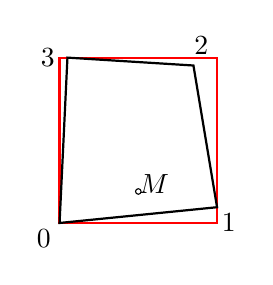
\begin{tikzpicture}
%\draw[step=0.5cm,gray,very thin] (0,0) grid (4,4); %background grid
\draw[thick,red] (1,1) -- (3,1) -- (3,3.1) -- (1,3.1) -- cycle;  
\draw[thick] (1,1) -- (3,1.2) -- (2.7,3) -- (1.1,3.1) -- cycle;  
\node[] at (0.8,0.8) {0};
\node[] at (3.15,1) {1};
\node[] at (2.8,3.25) {2};
\node[] at (0.85,3.1) {3};
\node[] at (2.2,1.5) {$M$};
\draw (2.,1.4) circle (1pt);
\end{tikzpicture}\\
\end{center}

Note that the algorithm above extends to high degree elements 
such as $Q_2$ and higher, even with curved sides.
As shown in the 2D case if the element is a cuboid or 
if all its lateral faces are vertical then one can 
compute the reduced coordinates without using an iterative method.


%-----------------------------------------------------
\subsubsection{Three-dimensional space - special case}

We assume that the mesh is such that the cross section of all $Q_1$ elements 
is a rectangle in the $xy$-plane. 

Let $(x,y,z)$ be a point inside the element. 
The global coordinates $x,y,z$ are obtained from the 
reduced coordinates $r,s,t$ via the basis the basis functions:
\begin{eqnarray}
x=\sum_{i=1}^8 \bN_i (r,s,t) x_i \qquad 
y=\sum_{i=1}^8 \bN_i (r,s,t) y_i  \qquad 
z=\sum_{i=1}^8 \bN_i (r,s,t) z_i \label{xyz}
\end{eqnarray}
Let 
\begin{eqnarray}
{\vec v}_1 &=& (+1,+1,+1,+1,+1,+1,+1,+1) \nn\\
{\vec v}_2 &=& (-1,+1,+1,-1,-1,+1,+1,-1) \nn\\
{\vec v}_3 &=& (-1,-1,+1,+1,-1,-1,+1,+1) \nn\\
{\vec v}_4 &=& (-1,-1,-1,-1,+1,+1,+1,+1) \nn\\
{\vec v}_5 &=& (+1,-1,+1,-1,+1,-1,+1,-1) \nn\\
{\vec v}_6 &=& (+1,-1,-1,+1,-1,+1,+1,-1) \nn\\
{\vec v}_7 &=& (+1,+1,-1,-1,-1,-1,+1,+1) \nn
\end{eqnarray}
and 
\begin{eqnarray}
{\vec x} &=& (x_1,x_2,x_3,x_4,x_5,x_6,x_7,x_8) \nn\\
{\vec y} &=& (y_1,y_2,y_3,y_4,y_5,y_6,y_7,y_8) \nn\\
{\vec z} &=& (z_1,z_2,z_3,z_4,z_5,z_6,z_7,z_8) \nn
\end{eqnarray}
then Eqs.~\eqref{xyz} can also be written
\begin{eqnarray}
x&=&\frac{1}{8} \left( {\vec v}_1 + r  {\vec v}_2 + s  {\vec v}_3 + t  {\vec v}_4 
                 + rs  {\vec v}_5 + rt {\vec v}_6 + st {\vec v}_7 \right) \cdot {\vec x} \nn\\ 
y&=&\frac{1}{8} \left( {\vec v}_1 + r  {\vec v}_2 + s  {\vec v}_3 + t  {\vec v}_4 
                 + rs  {\vec v}_5 + rt {\vec v}_6 + st {\vec v}_7 \right) \cdot {\vec y} \nn\\
z&=&\frac{1}{8} \left( {\vec v}_1 + r  {\vec v}_2 + s  {\vec v}_3 + t  {\vec v}_4 
                 + rs  {\vec v}_5 + rt {\vec v}_6 + st {\vec v}_7 \right) \cdot {\vec z} \label{zzz}
\end{eqnarray}
If the element has a rectangular cross-section $s_x \times s_y$ then 
\begin{eqnarray}
{\vec x} &=& (x_0,x_0+s_x,x_0+s_x,x_0,x_0,x_0+s_x,x_0+s_x,x_0) \nn\\
{\vec y} &=& (y_0,y_0,y_0+s_y,y_0+s_y,y_0,y_0,y_0+s_y,y_0+s_y) \nn
\end{eqnarray}
which yields
\begin{eqnarray}
r&=& 2\frac{x-x_0}{s_x}-1  \nn\\
s&=& 2\frac{y-y_0}{s_y}-1  \nn
\end{eqnarray}
Since the local coordinates $r$ and $s$ can be easily computed, one can use Eq.~\eqref{zzz} to obtain $t$:
\[
t=\frac{8z - ({\vec v}_1 + r {\vec v}_2 + s {\vec v}_3 + rs  {\vec v}_5 ) \cdot {\vec z}} 
{ ({\vec v}_4  + r  {\vec v}_6 + s  {\vec v}_7)  \cdot {\vec z} }
\]







 %------------
\newpage %-----------------------------------------------------------------------------------------
\section{Error measurements and convergence rates} \index{general}{$L_1$ norm}
\index{general}{$L_2$ norm}
\index{general}{$H^1$ norm}
\begin{flushright} {\tiny {\color{gray} errors.tex}} \end{flushright}

What follows is written in the case of a two-dimensional model. Generalisation to
3D is trivial. What follows is mostly borrowed from \cite{thmk14}.

When measuring the order of accuracy of the primitive variables $\vec{v}$ and $p$,
it is standard to report errors in both the $L_1$ and the $L_2$ norm.
For a scalar quantity $\Psi$, the $L_1$ and $L_2$ norms are computed as
\begin{equation}
\norm{\Psi}_1 = \int_V |\Psi| dV
\quad\quad
\quad\quad
\norm{\Psi}_2 = \sqrt{ \int_V \Psi^2 dV }
\end{equation}
For a vector quantity $\vec{k}=(k_x,k_y)$ in a two-dimensional space,
the $L_1$ and $L_2$ norms are defined as:
\begin{equation}
\norm{\vec{k}}_1 = \int_V (|k_x|+|k_y|) dV
\quad\quad
\quad\quad
\norm{\vec{k}}_2 = \sqrt{ \int_V (k_x^2+k_y^2) dV }
\end{equation}
To compute the respective norms
the integrals in the above norms can be approximated by splitting them
into their element-wise contributions. The element volume integral can then
be easily computed by numerical integration using Gauss-Legendre quadrature.

The respective $L_1$ and $L_2$ norms for the pressure error can be evaluated via
\begin{equation}
e_p^h|_1 = \sum_{i=1}^{n_e} \sum_{q=1}^{n_q} |e_p^h(\vec{r}_q)| w_q |J_q|
\quad\quad
\quad\quad
e_p^h|_2=\sqrt{ \sum_{i=1}^{n_e} \sum_{q=1}^{n_q} |e_p^h(\vec{r}_q)|^2 w_q |J_q| }
\end{equation}
where $e_p^h(\vec{r}_q)=p^h(\vec{r}_q) - p(\vec{r}_q)$ 
is the pressure error evaluated at the $q$-th quadrature associated with
the $i$th element. $n_e$ and $n_q$ refer to the number of elements and
the number of quadrature points per element.
$w_q$ and $J_q$ are the quadrature weight and the Jacobian associated with
point $q$.

The velocity error $e_{\vec v}^h$ is evaluated using the following two norms
\begin{equation}
e_{\vec{v}}^h|_1 = \sum_{i=1}^{n_e} \sum_{q=1}^{n_q} [ |e_u^h(\vec{r}_q)| + |e_v^h(\vec{r}_q)| ]    w_q |J_q|
\quad\quad
\quad\quad
e_{\vec v}^h|_2=\sqrt{ \sum_{i=1}^{n_e} \sum_{q=1}^{n_q} \left[ |e_u^h({\bm r}_q)|^2 +  e_v^h({\bm r}_q)|^2 \right] w_q |J_q| }
\end{equation}
where $e_u^h(\vec{r}_q)=u^h(\vec{r}_q) - u(\vec{r}_q)$ and $e_v^h(\vec{r}_q)=v^h(\vec{r}_q)-v(\vec{r}_q)$.


\index{general}{$H^1(\Omega)$ space} 
\index{general}{$H^1$ norm} 
\index{general}{$H^1$ semi-norm}
Another norm is very rarely used in the geodynamics literature but is preferred in the 
Finite Element literature: the $H^1$ norm. The mathematical basis for this
norm and the nature of the $H^1(\Omega)$ Hilbert space is to be found in many FE books \cite{dohu03,john16,hugh}.
This norm is expressed as follows for a function $f$ such that $f,|\nabla f|\in L^2(\Omega)$
\footnote{\url{https://en.wikipedia.org/wiki/Sobolev_space}}
\begin{equation}
\norm{f}_{H^1} = \left( \int_\Omega ( |f|^2 + |\nabla f|^2  ) d\Omega   \right)^{1/2}
\end{equation}
We then have 
\begin{equation}
e_{\vec v}^h|_{H^1} = \norm{\vec{v}^h-\vec{v}}_{H^1} = \sqrt{
\sum\limits_{i=1}^d 
\int_\Omega  
\left[
({v}_i^h-{v}_i)^2
+
\vec\nabla(v_i^h-v_i)\cdot\vec\nabla(v_i^h-v_i) 
\right] d\Omega   
}
\end{equation}
where $d$ is the number of dimensions.
Note that sometimes the following semi-norm is used \cite{dobo04,bodg06}:
\begin{equation}
e_{\vec v}^h|_{H^1} = \norm{\vec{v}^h-\vec{v}}_{H^1} = \sqrt{
\sum\limits_{i=1}^d 
\int_\Omega  
\left[
\vec\nabla(v_i^h-v_i)\cdot\vec\nabla(v_i^h-v_i) 
\right] d\Omega   
}
\end{equation}

When computing the different error norms for $e_p$ and $e_{\vec v}$ for a set of numerical experiments with
varying resolution $h$ we expect the error norms to follow the following relationships:
\begin{equation}
e_{\vec v}^h|_1 = C h^{rvL_1} 
\quad\quad\quad\quad
e_{\vec v}^h|_2 = C h^{rvL_2} 
\quad\quad\quad\quad 
e_{\vec v}^h|_{H^1} = C h^{rvH^1}
\end{equation}
\begin{equation}
e_p^h|_1 = C h^{rpL_1} 
\quad\quad\quad 
e_p^h|_2 = C h^{rpL_2}
\end{equation}
where $C$ is a resolution-independent constant
and $rpXX$ and $rvXX$ are the convergence rates for
pressure and velocity in various norms, respectively. 
Using linear regression on the logarithm of the respective error norm and the resolution $h$,
one can compute the convergence rates of the numerical solutions.

As mentioned in \cite{dobo04}, when finite element solutions converge at
the same rates as the interpolants we say that the method is optimal, i.e.:
\index{general}{optimal rate}

\begin{equation}
e_{\vec v}^h|_{L_2} = {\cal O}(h^3)
\quad\quad\quad\quad
e_{\vec v}^h|_{H^1} = {\cal O}(h^2)
\quad\quad\quad\quad
e_{p}^h|_{L_2} = {\cal O}(h^2)
\end{equation}

%\begin{itemize}
%\item For $Q_1P_0$, the theoretical lower bound for $r_v'$ is 2 and for $r_p'$ it is 1
%\item For $Q_2P_{-1}$, the theoretical lower bound for $r_v'$ is 3 and for $r_p'$ it is 2
%\end{itemize}
We note that when using discontinuous pressure space
(e.g., $P_0$, $P_{-1}$), these bounds remain valid even
when the viscosity is discontinuous provided that the element boundaries conform to the discontinuity.

%------------------------------------------------------------------------------ 
\subsubsection{About extrapolation}\label{ss:extrapolation}
\index{general}{Extrapolation}

Section contributed by W. Bangerth and part of \textcite{thba22} (2022) 
but it was ultimately not used. 

In a number of numerical benchmarks we
want to estimate the error $X_h-X^\ast$ between a quantity $X_h$ computed
from the numerical solution $\vec{\upnu}_h,p_h$ and the corresponding value
$X$ computed from the exact solution $\vec{\upnu},p$. Examples of such quantities
$X$ are the root mean square velocity $\upnu_{rms}$, but it could also be a mass flux
across a boundary, an average horizontal velocity at the top boundary, or
any other scalar quantity.

If the exact solution is known, then one can of course compute $X$ from it.
On the other hand, we would of course like to assess convergence also in
cases where the exact solution is not known. In that case, one can compute
an \textit{estimate} $X^\ast$ for $X$ by way of \textit{extrapolation}.
To this end, we make the assumption that asymptotically, $X_h$ converges to
$X$ at a fixed (but unknown) rate $r$, so that
\begin{equation}
  \label{eq:extrapolation-1}
  e_h=|X_h-X| \approx C h^r.
\end{equation}
Here, $X$, $C$ and $r$ are all unknown constants to be determined, although
we are not really interested in $C$.
We can evaluate $X_h$ from the numerical solution
on successively refined meshes with mesh sizes $h$, $h/2$, and $h/4$. Then,
in addition to \eqref{eq:extrapolation-1} we also have
\begin{eqnarray}
  \label{eq:extrapolation-2}
  e_{h/2}=|X_{h/2}-X| \approx C \left(\frac h2\right)^r,
  \\
  \label{eq:extrapolation-3}
  e_{h/4} =|X_{h/4}-X| \approx C \left(\frac h4\right)^r.
\end{eqnarray}
Taking ratios of equations \eqref{eq:extrapolation-1}--\eqref{eq:extrapolation-3},
and replacing the unknown $X$ by an \textit{estimate} $X^\ast$, we then
arrive at the following equation:
\begin{equation*}
\frac{|X_h-X^\star|}{|X_{h/2}-X^\star|}
=
\frac{|X_{h/2}-X^\star|}{|X_{h/4}-X^\star|}=2^r.
\end{equation*}
If one assumes that $X_h$ converges to $X$ uniformly either from above or
below (rather than oscillate around $X$), then this equation allows us
to solve for $X^\ast$ and $r$:

\[
(X_h-X^\star)(X_{h/4}-X^\star)=(X_{h/2}-X^\star)(X_{h/2}-X^\star)
\]

\[
X_h X_{h/4} -X^\star  X_{h/4} - X_h X^\star  + (X^\star)^2
=X_{h/2}^2 -2 X^\star X_{h/2} + (X^\star)^2 
\]

\[
X_h X_{h/4} -X^\star  X_{h/4} - X_h X^\star 
=X_{h/2}^2 -2 X^\star X_{h/2} 
\]

\[
X_h X_{h/4} -X_{h/2}^2 =-2 X^\star X_{h/2} +X^\star  X_{h/4} + X_h X^\star 
\]

\[
X_h X_{h/4} -X_{h/2}^2  = X^\star ( -2  X_{h/2}  +   X_{h/4} + X_h )
\]

and finally:
\begin{equation*}
X^\star = \frac{X_h X_{h/4}-X_{h/2}^2}{X_h - 2 X_{h/2} + X_{h/4}}, \qquad\qquad
r = \log_2 \frac{X_{h/2}-X^\star}{X_{h/4}-X^\star}.
\end{equation*}
In the determination of $r$, we could also have used $X_h$ and $X_{h/2}$,
but using $X_{h/2}$ and $X_{h/4}$ is generally more reliable because
the higher order terms we have omitted in \eqref{eq:extrapolation-1} are less
visible on finer meshes.

In some cases, however, halving the mesh size multiple times 
is not really tractable (memory problem, or cpu time).
Let us now start again from 
\begin{equation}
  e_h=|X_h-X| \approx C h^r.
\end{equation}
and assume that we run two other models at a resolution $\alpha h$
and $\beta h$, such that $1>\alpha>\beta>0$. 
In the example above we of course had $\alpha=1/2$ and $\beta=1/4$.
Then we have 
\begin{eqnarray}
e_{\alpha h}=|X_{\alpha h}-X| \approx C \left(\alpha h\right)^r,  \\
e_{\beta  h}=|X_{\beta h} -X| \approx C \left(\beta  h\right)^r.
\end{eqnarray}
which leads to 
\begin{equation*}
\frac{|X_h-X^\star|}{|X_{\alpha h}-X^\star|}
= \frac{C h^r}{C (\alpha h)^r} = (1/\alpha)^{r}
\qquad
\text{and}
\qquad
\frac{|X_{\alpha h}-X^\star|}{|X_{\beta h}-X^\star|}
= \frac{C (\alpha h)^r}{C(\beta h)^r} = (\alpha/\beta)^r
\end{equation*}
In order for both to be equal we must have
\[
(1/\alpha)^{r} = (\alpha/\beta)^r
\qquad
\Rightarrow
\qquad
1/\alpha = \alpha/\beta
\qquad
\Rightarrow
\qquad
\beta=\alpha^2
\]
So of course if $\alpha=1/2$ then $\beta=1/4$, but now we can also take 
$\alpha=3/4$ and then $\beta=9/16$. Etc ...

In the end, this approach might not be that useful since the mesh sizes would
then be $h,3h/4,9h/16,27h/64,...$ which may be hard to achieve in practice.

 %--------------------------------
\newpage %-----------------------------------------------------------------------------------------
\section{The initial temperature field} 
\Literature: 
\begin{itemize}
\item
Thermal gradients in the continental crust \cite{chap86}
\item
Simple analytical approximation to the temperature structure in
subduction zones \cite{enwi04}
\item 
Thermal structure of subduction zone back arcs \cite{cuhy06}
\item 
Thermal Structure of Oceanic Lithosphere \cite{rihc18}
\item thermal structure of a subducting plate with finite length \cite{hstt90}
\end{itemize}


%.............................................................
\subsubsection{Single layer with imposed temperature b.c.}

Let us take a single layer of material characterised by
a heat capacity $C_p$, a heat conductivity $k$
and a heat production term $H$.

\begin{center}
\includegraphics[width=5cm]{images/initial_temperature/tempcond.png}
\end{center}

The Heat transport equation writes
\begin{equation}
\rho C_p \left( \frac{\partial T}{\partial t} + {\vec v} \cdot {\vec \nabla} { T} \right) = 
{\vec \nabla} \cdot (k {\vec \nabla} T) + \rho H
\end{equation}
At steady state and in the absence of a velocity field, assuming
that the material properties to be independent of time and space, and 
assuming that
there is no heat production ($H=0$), this equation
simplifies to
\begin{equation}
\Delta T =0 
\end{equation}
Assuming the layer to be parallel to the $x$-axis, the temperature is
$T(x,y)=T(y)=\alpha T+ \beta$. 
In order to specify the constants $\alpha$ and $\beta$, we need two constraints.

At the bottom of the layer $y=y_b$ a temperature $T_b$ is prescribed while a temperature
$T_t$ is prescribed at the top with $y=y_t$. This ultimately yields a temperature field in
the layer given by
\begin{mdframed}[backgroundcolor=blue!5]
\[
T(y) = \frac{T_t-T_b}{y_t-y_b}(y-y_b) + T_b
\]
\end{mdframed}

If now the heat production coefficient is not zero, the differential equation
reads
\begin{equation}
 k \Delta T + H = 0 
\end{equation}
The temperature field is then expected to be of the form
\begin{equation}
T(y)= - \frac{H}{2k} y^2 + \alpha y + \beta 
\end{equation}
Supplied again with the same boundary conditions, this leads to
\[
\beta=T_b + \frac{H}{2k} y_b^2 - \alpha y_b
\]
ie,
\[
T(y) = -\frac{H}{2k} (y^2-y_b^2) + \alpha (y-y_b) + T_b
\]
and finally
\[
\alpha =  \frac{T_t-T_b}{y_t-y_b}  + \frac{H}{2k}(y_b+y_t)
\]
or,
\[
T(y) = -\frac{H}{2k} (y^2-y_b^2) + \left( \frac{T_t-T_b}{y_t-y_b}  + \frac{H}{2k}(y_b+y_t)   \right) (y-y_b) + T_b
\]

Taking $H=0$ in this equation obviously yields the temperature field obtained previously.
Taking $k=2.25$, $T_t=0C$, $T_b=550C$, $y_t=660km$, $y_b=630km$ yields the following
temperature profiles and heat fluxes when the heat production $H$ varies:
\begin{center}
\includegraphics[width=5cm]{images/initial_temperature/temperature1.pdf}
\includegraphics[width=5cm]{images/initial_temperature/heatflux1.pdf}
\end{center}
Looking at the values at the top, which are somewhat estimated to be
about $55-65mW/m^2$ \cite[table 8.6]{jama}, one sees that value $H=0.8e-6$ yields a very acceptable
heat flux.
Looking at the bottom, the heat flux is then about $0.03W/m^2$
which is somewhat problematic since the heat flux at the Moho
is reported to be somewhere between 10 and 20 $mW/m^2$ in \cite[table 7.1]{jama}.


%-----------------------------------------------------
\subsubsection{Single layer with imposed heat flux b.c.}

Let us now assume that heat fluxes are imposed at the top and bottom of the layer:
\begin{center} 
\includegraphics[width=5cm]{images/initial_temperature/tempcond2.png}
\end{center}

We start again from the ODE
\[
k \Delta T + H = 0 
\]
but only integrate it once:
\[
k \frac{dT}{dy}  + H y + \alpha  = 0 
\]
At the bottom $q=k(dT/dy)|_{y=y_b} = q_b$ and at the top
$q=k(dT/dy)|_{y=y_t} = q_t$ so that 

\todo[inline]{to finish}


 
%-----------------------------------------------------
\subsubsection{Single layer with imposed heat flux and temperature b.c. }

\begin{center}
\includegraphics[width=5cm]{images/initial_temperature/tempcond3.png}
\end{center}

\todo[inline]{to finish}


%---------------------------------------------------------------
\subsubsection{Half cooling space}

TODO. 

\Literature \cite{fagm12} 

%---------------------------------------------------------------
\subsubsection{Plate model}

\cite{mcke67}

%.................................
\subsubsection{McKenzie slab}

When doing thermo-mechanical modelling, the initial temperature
field in the domain is of prime importance. This is 
especially true for the temperature in the slab for subduction 
modelling as its rheological behaviour is strongly temperature-dependent. 
One could easily design a simple geometrical initial field but it is 
unlikely to be close to the field of a slowly subducting slab at an angle 
in a hot mantle. 

McKenzie \cite{mcke69} derived such approximate initial field from the 
steady-state energy equation in two dimensions:
\begin{equation}
\rho C_p \vec v \cdot \vec\nabla T = k \vec\nabla^2 T
\end{equation}
We denote by $T_l$ the temperature at the base of the lithosphere
and $l$ its thickness (i.e. the thickness of the slab).

Assuming $\vec v=(v_x,0)$ yields
\[
\rho C_p v_x \frac{\partial T}{\partial x} = k \frac{\partial^2 T}{\partial x^2}
\]
and substitution of $T'=T/T_l$, $x'=x/l$ and $z'=z/l\in[0,1]$ in this equation leads to
\[
\rho C_p v_x \frac{T_l}{l}\frac{\partial T'}{\partial x'} = k \frac{T_l}{l^2}
\left( \frac{\partial^2 T'}{\partial x'^2}
+ \frac{\partial^2 T'}{\partial z'^2} \right)
\]
or 
\[
\frac{\rho C_p v_x l }{k}\frac{\partial T'}{\partial x'} = 
\frac{\partial^2 T'}{\partial x'^2}
+ \frac{\partial^2 T'}{\partial z'^2} 
\]
and finally (see Eq. 2.3 of \cite{mcke69}): 
\[
\frac{\partial^2 T'}{\partial x'^2}
- 2 R \frac{\partial T'}{\partial x'} 
+ \frac{\partial^2 T'}{\partial z'^2} =0
\]
where $R$ is the thermal Reynolds number
\[
R=\frac{\rho C_p v_x l}{2 k}
\] 
The general solution to this PDE with $T'=1$ on the top, left and right boundary is 
\[
T'(x',z')= 1 + \sum_n C_n \exp \left[ \left( R-(R^2+n^2\pi^2)^{1/2} \right) x' \right] \sin (n \pi z')
\]
We now must make an assumption about the temperature on the left boundary ($x'=0$), 
which is the temperature of the lithosphere. 
For simplicity McKenzie assumes that $T'(x'=0,z')=1-z'$ so that $C_n=2(-1)^n/n\pi$ and finally
\begin{mdframed}[backgroundcolor=blue!5]
\begin{equation}
T'(x',z')= 1 + 2\sum_n \frac{(-1)^n}{n \pi} \exp \left[ \left( R-(R^2+n^2\pi^2)^{1/2} \right) x' \right] \sin (n \pi z')
\end{equation}
\end{mdframed}

Let us build a simple temperature model for a $250\text{km}\times 50\text{km}$ slab, 
with $\rho=3000$, $C_p=1250$, $k=3$. The python code is available in {\tt images/mckenzie/mckenzie1.py}.

\begin{center}
\includegraphics[width=0.32\textwidth]{images/mckenzie/temperature_vel0p5.pdf}
\includegraphics[width=0.32\textwidth]{images/mckenzie/temperature_vel1.pdf}
\includegraphics[width=0.32\textwidth]{images/mckenzie/temperature_vel2.pdf}\\
{\captionfont Left to right: Dimensionless temperature $T'$ in a $250\text{km}\times 50\text{km}$ slab 
for $v_x={0.5,1,2}\text{cm/year}$}
\end{center}

We logically recover the fact that the slower the slab penetrates the mantle the more 
temperature diffusion dominates over temperature advection. For $v=0.5\text{cm/year}$ we see that 
that the slab assumes a constant temperature $T'=1$ at all depthes $0\leq z' \leq 1$ for 
$x'\geq 125\text{km}$. 

Note that this field is a steady-state field, valid for a constant density, heat conductivity and 
heat capacity, zero heat production, that it implies that the velocity is constant and that the 
lithosphere temperature is linear. 

One can also embed the slab in a more realistic context, a subduction zone, involving a 
subducting lithosphere, an over-riding plate and a mantle. The domain is $1000\text{km}\times 250\text{km}$.
The mantle temperature is set to $1300~\si{\celsius}$. The slab dip can be varied and so can the 
velocity. The python code is available in {\tt images/mckenzie/mckenzie2.py}.

\begin{center}
\includegraphics[width=0.32\textwidth]{images/mckenzie/temperature2_vel0p5_phi30.pdf}
\includegraphics[width=0.32\textwidth]{images/mckenzie/temperature2_vel1_phi30.pdf}
\includegraphics[width=0.32\textwidth]{images/mckenzie/temperature2_vel2_phi30.pdf}\\
{\captionfont Left to right: temperature $T$ for $v_x={0.5,1,2}\text{cm/year}$ and $\phi=30\degree$.}
\end{center}

\begin{center}
\includegraphics[width=0.32\textwidth]{images/mckenzie/temperature2_vel1_phi15.pdf}
\includegraphics[width=0.32\textwidth]{images/mckenzie/temperature2_vel1_phi30.pdf}
\includegraphics[width=0.32\textwidth]{images/mckenzie/temperature2_vel1_phi45.pdf}\\
{\captionfont Left to right: temperature $T$ for $v_x=1\text{cm/year}$ and $\phi={15,30,45}\degree$.}
\end{center}




%\newpage

%From \cite{mcke70}, Eq. 26:
%\[
%T(r_0) = \theta_1 \exp \left(  \frac{\alpha g}{C_p} (r_1-r_0) \right)
%\]
%where $\theta_1$ is the potential temperature of any piece of the mantle 
%at the earth's surface.
%If $x$ is measured from a depth equal to the thickness of the lithosphere down the
%dip of the slab and $z$ is measured along the normal to the slab from its lower 
%surface, then the dimensionless potential temperature in the slab is 
%\begin{eqnarray}
%\theta'(x',z')
%&=& 1+2\frac{\theta_1-273}{\theta_1} \sum_{n=1}^\infty \frac{(-1)^n}{n \pi}
%\exp \left[ \left( R-(R^2+n^2\pi^2)^{1/2} \right) x' \right] \sin n\pi z' \\
%&=& \frac{1}{\theta_1} \left\{ \theta_1+ 2 (\theta_1-273) \sum_{n=1}^\infty \frac{(-1)^n}{n \pi}
%\exp \left[ \left( R-(R^2+n^2\pi^2)^{1/2} \right) x' \right] \sin n\pi z' \right\}
%\end{eqnarray}
%where $\theta' = \theta/\theta_1$, $x'=x/l$, $z'=z/l$ and 
%with $l$ the thickness of the slab and $v$ its velocity measured down its dip.
%We denote by $\phi$ the dip of the slab so that the depth below the surface $r_1-r_0$ is given by
%$l (x' \sin \phi-z' \cos\phi)$ so that 
%\[
%T(r_0) = \theta_1 \exp \left(  \frac{\alpha g}{C_p} l (x' \sin \phi-z' \cos\phi) \right)
%\]
%The dimensionless scale height $h'$ is defined by $h'=C_p/\alpha g l$ so that
%\[
%T(r_0) = \theta_1 \exp \left[  (x' \sin \phi-z' \cos\phi)/h' \right]
%\]

%Finally,
%\[
%T(x',z')=\exp \left[  (x' \sin \phi-z' \cos\phi)/h' \right] 
%\left\{ \theta_1+ 2 (\theta_1-273) \sum_{n=1}^\infty \frac{(-1)^n}{n \pi}
%\exp \left[ \left( R-(R^2+n^2\pi^2)^{1/2} \right) x' \right] \sin n\pi z' \right\}
%\]

%\todo[inline]{BSc: create mckenzie slab temperature setup}

%......................................................................
\subsubsection{Initial temperature for global mantle convection models}

This is a difficult topic, and Gottschaldt \etal \cite{gows09} list a few issues or 
facts to take into account:
\begin{itemize}
\item Frequent  impacts  may  have  determined  the  heat structure of the outer layers (Arrhenius and Lepland 2000), leading to an early thermally stable stratification. 
\item A global magma ocean (Solomatov 2000)  or  several  large  scale  melting events  (Kleine \etal. 2004)  
are also conceivable. 
\item Fractional crystallisation and subsequent overturn has the potential to result in 
compositionally or thermally stable layering, too (Elkins-Tanton \etal 2003; Zaranek and Parmentier 2004)
\end{itemize}


 %------------------------------
\newpage %-----------------------------------------------------------------------------------------
\section{The consistent boundary flux (CBF) \label{ss:cbf}} \begin{flushright} {\tiny {\color{gray} cbf.tex}} \end{flushright}

The Consistent Boundary Flux technique was devised to 
alleviate the problem of the accuracy of primary variables 
derivatives (mainly velocity and temperature) on boundaries.
These derivatives are important since they are needed to compute
the heat flux (and therefore the Nusselt number) or 
dynamic topography and geoid. 

The idea was first introduced in Mizukami (1986) \cite{mizu86} and later used 
in geodynamics in Zhong \etal (1993) \cite{zhgh93}. It was finally implemented 
in the \citcoms code \cite{zhmt08,mole97} and more recently
in the \aspect code (dynamic topography postprocessor).
Note that the CBF should be seen as a post-processor step 
as it does not alter the primary variables values.

The CBF method is implemented and used in \stone~27.
It is also discussed but not explicitely named in Reddy's book \cite[p309]{reddybook2}.
Also see Larock \& Herrmann (1976) \cite{lahe76}, Gresho \etal (1987) \cite{grls87}, Marshall \etal \cite{mahz78}.


%---------------------------------------------------------------
\subsection{The CBF applied to the Stokes equation}
We start from the strong form:
\begin{equation}
{\vec \nabla}\cdot {\bm \sigma} + {\vec b} = {\vec 0} 
\end{equation}
and then write the weak form on an element $e$:
\begin{equation}
\int_{\Omega_e} N_i^\upnu {\vec \nabla}\cdot {\bm \sigma}\; dV
+ \int_{\Omega_e} N_i^\upnu  {\vec b} \; dV
= \vec 0 
\end{equation}
We then use the two equations: 
\index{general}{Chain Rule} 
\index{general}{Divergence Theorem}
\[
\vec \nabla \cdot ( N  \bm \sigma ) = N \vec{\nabla} \cdot \bm \sigma + \vec{\nabla} N \cdot  \bm \sigma  
\qquad \text{(chain rule)}
\]
\[
\int_\Omega (\vec \nabla \cdot {\bm \sigma} )\; dV = \int_\Gamma {\bm \sigma} \cdot \vec{n} \; dS
\qquad \text{(divergence theorem)}
\]
and integrate by parts in order to obtain:
\begin{eqnarray}
\int_\Gamma N_i^\upnu {\bm \sigma}\cdot\vec{n} \; dS - 
\int_{\Omega_e} {\vec \nabla } N_i^\upnu \cdot {\bm \sigma} \; dV 
+ \int_{\Omega_e} N_i^\upnu  {\vec b} \; dV =\vec{0}
\end{eqnarray}
and since the traction vector ${\vec t}$ is given by $\vec{t}={\bm \sigma}\cdot\vec{n}$ we have:
\begin{eqnarray}
\int_{\Gamma_e}  N_i^\upnu {\vec t} \; dS 
&=& \int_{\Omega_e} {\vec \nabla } N_i^\upnu \cdot {\bm \sigma}\; dV 
- \int_{\Omega_e} N_i^\upnu  {\vec b} \; dV   \label{eq:cbf1}
\end{eqnarray}
The core idea of the method lies in considering the traction vector as an unknown 
living on the nodes on the boundary, and assuming we have already solved the Stokes 
equation and therefore have obtained the velocity and pressure.

Finally, since the traction vector can be expressed as a function of the velocity 
basis functions on the edge i.e.
\[
\vec{t} = \sum_{i=1}^m N_i^\upnu \vec{t}_i
\]
the left hand term yields an edge (1D) mass matrix $\M'$ (see Section~\ref{app:mm}).

\begin{remark}
In \stone~27 an alternative to equation \ref{eq:cbf1} is used. Although
somewhat inefficient, the elemental matrices $\K$ and $\G$ and the corresponding 
body force rhs are built and the rhs of the traction equation is computed as follows:
\[
\M' \cdot \vec{\cal T} = -\K \cdot \vec{\cal V} - \G \cdot\vec{\cal P} + \vec{f}
\]
where $\vec{\cal T}$ is the vector of assembled tractions which we want to compute 
and $\vec{\cal V}$ and $\vec{\cal T}$ are the solutions of the Stokes problem. 
\end{remark}

\begin{remark} 
The assembled mass matrix is tri-diagonal and can be easily solved with 
a Conjugate Gradient method. 
\end{remark}

\begin{remark} 
With a trapezoidal integration rule 
(i.e. Gauss-Lobatto - see Section~\ref{sec:loba}) the matrix can even be diagonalised and the resulting 
matrix is simply diagonal, which results in a very cheap solve as mentioned in Zhong \etal (1993) \cite{zhgh93}.
\end{remark}







\subsubsection{Some implementation details for the Stokes equation}

What follows is relevant for \stone~27 which relies on $Q_1$ shape 
functions for the velocity. 
Let us start with a small example, a 3x2 element FE grid:
\begin{center}
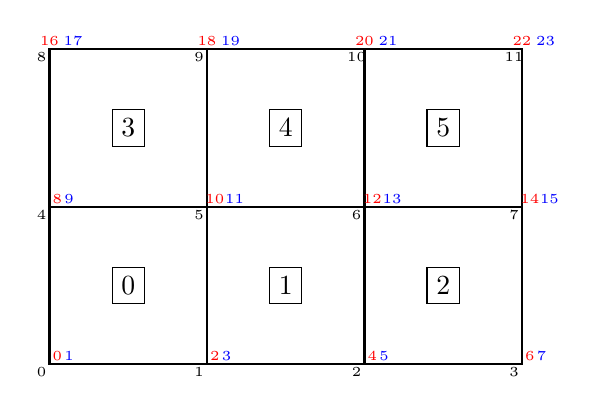
\begin{tikzpicture}
%\draw[step=0.5cm,gray,very thin] (0,0) grid (8,6); %background grid
\draw[thick] (1,1) -- (3,1) -- (3,3) -- (1,3) -- cycle;  
\draw[thick] (3,1) -- (5,1) -- (5,3) -- (3,3) -- cycle; 
\draw[thick] (5,1) -- (7,1) -- (7,3) -- (5,3) -- cycle; 
\draw[thick] (1,3) -- (3,3) -- (3,5) -- (1,5) -- cycle;  
\draw[thick] (3,3) -- (5,3) -- (5,5) -- (3,5) -- cycle; 
\draw[thick] (5,3) -- (7,3) -- (7,5) -- (5,5) -- cycle; 
\node[draw] at (2,2) {0};
\node[draw] at (4,2) {1};
\node[draw] at (6,2) {2};
\node[draw] at (2,4) {3};
\node[draw] at (4,4) {4};
\node[draw] at (6,4) {5};
%pressure dofs
\node at (0.9,0.9) {\tiny 0};
\node at (2.9,0.9) {\tiny 1};
\node at (4.9,0.9) {\tiny 2};
\node at (6.9,0.9) {\tiny 3};
\node at (0.9,2.9) {\tiny 4};
\node at (2.9,2.9) {\tiny 5};
\node at (4.9,2.9) {\tiny 6};
\node at (6.9,2.9) {\tiny 7};
\node at (0.9,4.9) {\tiny 8};
\node at (2.9,4.9) {\tiny 9};
\node at (4.9,4.9) {\tiny 10};
\node at (6.9,4.9) {\tiny 11};
%velocity dofs
\node[red] at (1.1,1.1) {\tiny 0};  \node[blue] at (1.25,1.1) {\tiny 1};
\node[red] at (3.1,1.1) {\tiny 2};  \node[blue] at (3.25,1.1) {\tiny 3};
\node[red] at (5.1,1.1) {\tiny 4};  \node[blue] at (5.25,1.1) {\tiny 5};
\node[red] at (7.1,1.1) {\tiny 6};  \node[blue] at (7.25,1.1) {\tiny 7};
\node[red] at (1.1,3.1) {\tiny 8};  \node[blue] at (1.25,3.1) {\tiny 9};
\node[red] at (3.1,3.1) {\tiny 10}; \node[blue] at (3.35,3.1) {\tiny 11};
\node[red] at (5.1,3.1) {\tiny 12}; \node[blue] at (5.35,3.1) {\tiny 13};
\node[red] at (7.1,3.1) {\tiny 14}; \node[blue] at (7.35,3.1) {\tiny 15};
\node[red] at (1.,5.1) {\tiny 16}; \node[blue] at (1.3,5.1) {\tiny 17};
\node[red] at (3.,5.1) {\tiny 18}; \node[blue] at (3.3,5.1) {\tiny 19};
\node[red] at (5.,5.1) {\tiny 20}; \node[blue] at (5.3,5.1) {\tiny 21};
\node[red] at (7.,5.1) {\tiny 22}; \node[blue] at (7.3,5.1) {\tiny 23};
\end{tikzpicture}\\
{\tiny Red color corresponds to the dofs in the x direction, blue color indicates a dof in the y direction.}
\end{center}

We have nnp=12, nel=6, NfemV=24. Let us assume that free slip boundary conditions are applied. 
The boundary conditions {\tt fix\_bc} array is then:
\begin{center}
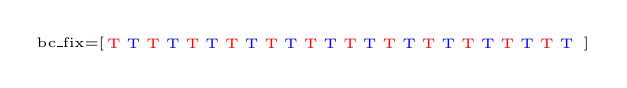
\begin{tikzpicture}
%\draw[step=0.5cm,gray,very thin] (0,0) grid (9,0.7); %background grid
\node  at (0.45,.1) {\tiny bc\_fix=[};

\node[red]  at (1.00,.1) {\tiny T};
\node[blue] at (1.25,.1) {\tiny T};
\node[red]  at (1.50,.1) {\tiny T};
\node[blue] at (1.75,.1) {\tiny T};
\node[red]  at (2.00,.1) {\tiny T};
\node[blue] at (2.25,.1) {\tiny T};
\node[red]  at (2.50,.1) {\tiny T};
\node[blue] at (2.75,.1) {\tiny T};
\node[red]  at (3.00,.1) {\tiny T};
\node[blue] at (3.25,.1) {\tiny T};
\node[red]  at (3.50,.1) {\tiny T};
\node[blue] at (3.75,.1) {\tiny T};
\node[red]  at (4.00,.1) {\tiny T};
\node[blue] at (4.25,.1) {\tiny T};
\node[red]  at (4.50,.1) {\tiny T};
\node[blue] at (4.75,.1) {\tiny T};
\node[red]  at (5.00,.1) {\tiny T};
\node[blue] at (5.25,.1) {\tiny T};
\node[red]  at (5.50,.1) {\tiny T};
\node[blue] at (5.75,.1) {\tiny T};
\node[red]  at (6.00,.1) {\tiny T};
\node[blue] at (6.25,.1) {\tiny T};
\node[red]  at (6.50,.1) {\tiny T};
\node[blue] at (6.75,.1) {\tiny T};

\node  at (7,.1) {\tiny ]};

\end{tikzpicture}\\
\end{center}
Note that since corners belong to two edges, we effectively prescribed 
no-slip boundary conditions on those. 
\todo[inline]{why does array contain only T??}


We wish to compute the tractions on the boundaries, and more precisely for the dofs for which 
a Dirichlet velocity boundary condition has been prescribed.
The number of (traction) unknowns NfemTr is then the number of {\tt T} in the {\tt bc\_fix} array.
In our specific case, we wave NfemTr= .
\todo{finish}
This means that we need for each targeted dof to be able to find its identity/number
between 0 and NfemTr-1. We therefore create the array {\tt bc\_nb} which is 
filled as follows: 
 
\begin{center}
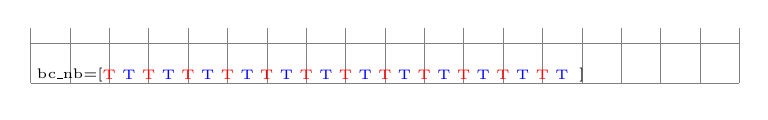
\begin{tikzpicture}
\draw[step=0.5cm,gray,very thin] (0,0) grid (9,0.7); %background grid

\node  at (0.5,.1) {\tiny bc\_nb=[};

\node[red]  at (1.00,.1) {\tiny T};
\node[blue] at (1.25,.1) {\tiny T};
\node[red]  at (1.50,.1) {\tiny T};
\node[blue] at (1.75,.1) {\tiny T};
\node[red]  at (2.00,.1) {\tiny T};
\node[blue] at (2.25,.1) {\tiny T};
\node[red]  at (2.50,.1) {\tiny T};
\node[blue] at (2.75,.1) {\tiny T};
\node[red]  at (3.00,.1) {\tiny T};
\node[blue] at (3.25,.1) {\tiny T};
\node[red]  at (3.50,.1) {\tiny T};
\node[blue] at (3.75,.1) {\tiny T};
\node[red]  at (4.00,.1) {\tiny T};
\node[blue] at (4.25,.1) {\tiny T};
\node[red]  at (4.50,.1) {\tiny T};
\node[blue] at (4.75,.1) {\tiny T};
\node[red]  at (5.00,.1) {\tiny T};
\node[blue] at (5.25,.1) {\tiny T};
\node[red]  at (5.50,.1) {\tiny T};
\node[blue] at (5.75,.1) {\tiny T};
\node[red]  at (6.00,.1) {\tiny T};
\node[blue] at (6.25,.1) {\tiny T};
\node[red]  at (6.50,.1) {\tiny T};
\node[blue] at (6.75,.1) {\tiny T};
\node  at (7,.1) {\tiny ]};
\end{tikzpicture}\\
\end{center}

This translates as follows in the code:
\begin{lstlisting}
NfemTr=np.sum(bc_fix)
bc_nb=np.zeros(NfemV,dtype=np.int32)
counter=0
for i in range(0,NfemV):
    if (bc_fix[i]):
       bc_nb[i]=counter
       counter+=1
\end{lstlisting}


The algorithm is then as follows

\begin{itemize}
\item[A] Prepare two arrays to store the matrix $M_{cbf}$ and its right hand side $rhs_{cbf}$  

\item[B] 
Loop over all elements 

\item[C] 
For each element touching a boundary, compute the residual vector 
$R_{el}=-f_{el} + \K_{el}{\cal V}_{el} + \G_{el} {\cal P}_{el}$

\item[D]
Loop over the four edges of the element using the connectivity array

\item[E]
For each edge loop over the number of degrees of freedom (2 in 2D)

\item[F] 
For each edge assess whether the dofs on both ends are target dofs. 

\item[G]
If so, compute the mass matrix $M_{edge}$ for this edge 

\item[H] extract the 2 values off the element residual vector and assemble these
in $rhs_{cbf}$

\item[I] Assemble $M_{edge}$ into NfemTrxNfemTr matrix using bc\_nb
\end{itemize}


\begin{lstlisting}
M_cbf = np.zeros((NfemTr,NfemTr),np.float64)         # A
rhs_cbf = np.zeros(NfemTr,np.float64)

for iel in range(0,nel):                             # B

    ... compute elemental residual ...               # C

    #boundary 0-1                                    # D
    for i in range(0,ndofV):                         # E
        idof0=2*icon[0,iel]+i
        idof1=2*icon[1,iel]+i
        if (bc_fix[idof0] and bc_fix[idof1]):        # F
           idofTr0=bc_nb[idof0]   
           idofTr1=bc_nb[idof1]
           rhs_cbf[idofTr0]+=res_el[0+i]             # H
           rhs_cbf[idofTr1]+=res_el[2+i]              
           M_cbf[idofTr0,idofTr0]+=M_edge[0,0]       # 
           M_cbf[idofTr0,idofTr1]+=M_edge[0,1]       # I
           M_cbf[idofTr1,idofTr0]+=M_edge[1,0]       # 
           M_cbf[idofTr1,idofTr1]+=M_edge[1,1]       #

    #boundary 1-2                                    #[D]

    ...

    #boundary 2-3                                    #[D]

    ...

    #boundary 3-0                                    #[D]

    ...


\end{lstlisting}










%---------------------------------------------------------------
\subsection{The CBF applied to the heat transport equation}

We start from the strong form of the heat transfer equation (without the source terms for simplicity):
\[
\rho C_p
\left(\frac{\partial T}{\partial t} + \vec{\upnu}\cdot \vec{\nabla}T\right)
=
\vec{\nabla} \cdot k\vec{\nabla} T
\]
The weak form then writes:
\[
\int_\Omega \bN^\uptheta
\rho C_p
\frac{\partial T}{\partial t} dV 
+
\int_\Omega \bN^\uptheta
\rho C_p
\vec{\upnu}\cdot \vec{\nabla}T  dV
=
\int_\Omega \bN^\uptheta
\vec{\nabla} \cdot k\vec{\nabla} T dV
\]
Using once again integration by parts and divergence theorem:
\[
\int_\Omega \bN^\uptheta
\rho C_p
\frac{\partial T}{\partial t} dV 
+
\int_\Omega \bN^\uptheta
\rho C_p
\vec{\upnu}\cdot \vec{\nabla}T  dV
=
\int_\Gamma \bN^\uptheta k \vec{\nabla} T \cdot \vec{n} d\Gamma
-
\int_\Omega  \vec{\nabla} \bN^\uptheta \cdot k \vec{\nabla} T dV
\]
On the boundary we are interested in the heat flux $\vec{q}=-k \vec{\nabla} T$
\[
\int_\Omega \bN^\uptheta
\rho C_p
\frac{\partial T}{\partial t} dV 
+
\int_\Omega \bN^\uptheta
\rho C_p
\vec{\upnu}\cdot \vec{\nabla} T  dV
=
-\int_\Gamma \bN^\uptheta {\bm q} \cdot {\bm n} d\Gamma
- \int_\Omega  \vec{\nabla} \bN^\uptheta \cdot k \vec{\nabla} T dV
\]
or,
\[
\int_\Gamma \bN^\uptheta {\bm q} \cdot {\bm n} d\Gamma
=
-\int_\Omega \bN^\uptheta
\rho C_p
\frac{\partial T}{\partial t} dV 
-
\int_\Omega \bN^\uptheta
\rho C_p  {\bm v}\cdot \vec{\nabla} T  dV
- \int_\Omega  \vec{\nabla} \bN^\uptheta \cdot k \vec{\nabla} T dV
\]
Considering the normal heat flux $q_n = \vec{q} \cdot \vec{n}$ as an unknown 
living on the nodes on the boundary, 
\[
q_n = \sum_{i=1}^2 q_{n|i} N_i
\]
so that the left hand term becomes a mass matrix for the basis functions living on 
the boundary.
We have already covered the right hand side terms when building the FE system 
to solve the heat transport equation, so that in the end 
\[
\M' \cdot \vec{\cal Q}_n =
- \M \cdot \frac{\partial \bm T}{\partial t} -K_a \cdot {\bm T} - K_d \cdot {\bm T} 
\]
where $\vec{\cal Q}_n$ is the assembled vector of normal heat flux components.
Note that in all terms the assembly only takes place over the elements along the boundary.


Note that the resulting matrix is symmetric.


 %--------------------------
\newpage %-----------------------------------------------------------------------------------------
\section{Computing gradients - the recovery process \label{ss:gradrecovery}} \begin{flushright} {\tiny {\color{gray} \tt recovery.tex}} \end{flushright}
%~~~~~~~~~~~~~~~~~~~~~~~~~~~~~~~~~~~~~~~~~~~~~~~~~~~~~~~~~~~~~~~~~~~~~~~~~~~~~~~~~~~~~~~~~~~~~~~~~~

write about recovering accurate strain rate components and heat flux components on the nodes.

Let $\vec g(\vec r)$  be the desired nodal 
field which we want to be the continuous (for example $Q_1$) 
representation of the field $\vec \nabla f^h$.
Since the derivative of the basis function does not uniquely exist on the nodes we need to design
an algorithm to do so. This problem is well known and has been investigated 
\todo{refs!}.
The main standard techniques are listed hereafter.

\Literature: check \fullcite{zibz98}

%..............................
\subsubsection{Global recovery}

The global recovery approach is rather simple: we wish to find $\vec g^h$
such that it satisfies
\[
\int_\Omega \phi \vec g^h \; d\Omega  = \int_\Omega \phi \vec\nabla f^h \; d\Omega 
\quad\quad \forall \phi
\] 
We will then successively replace $\phi$ by all the basis functions $N_i$ 
and since we have $g^h=\sum_j N_i g_i$ we then obtain
\[
\sum_j \int N_i N_j d\Omega g_i = \int N_i  \vec\nabla f^h \; d\Omega 
\]
or, 
\[
\mathbb{M} \cdot \vec{\cal G} = \vec f
\]



%..................................................
\subsubsection{Local recovery - centroid average over patch}





%..................................................
\subsubsection{Local recovery - nodal average over patch}

Let $j$ be the node at which we want to compute $\vec g$.
Then 
\[
\vec g_j = \vec g(\vec r_j) = 
\frac{\sum\limits_{ e \text{ adj. to }j} |\Omega_e| (\vec\nabla f)_e(\vec r_j) }{\sum |\Omega_e|}
\]
where $|\Omega_e|$ is the volume of the element and $(\vec\nabla f^h)_e(\vec r_j)$
is the gradient of $f$ as obtained with the basis functions inside element $e$ and 
computed at location $\vec r_j$.

%........................................................
\subsubsection{Local recovery - least squares over patch}



%........................................................
\subsubsection{Link to pressure smoothing}

When the penalty method is used to solve the Stokes equation, the pressure
is then given by $p=-\lambda \vec\nabla \cdot \vec v$. As explained in 
section \ref{sec:penalty}, the velocity is first obtained and the pressure 
is recovered by using this equation as a postprocessing step. Since the divergence 
cannot be computed easily at the nodes, the pressure is traditionally computed 
in the middle of the elements, yielding an elemental pressure field (remember, 
we are talking about $Q_1P_0$ elements here -- bi/tri-linear velocity, discontinuous
constant pressure)


 %----
\newpage %-----------------------------------------------------------------------------------------
\section{Tracking materials and/or interfaces} \begin{flushright} {\tiny {\color{gray} \tt tracking.tex}} \end{flushright}

Unless using a fully Lagrangian formulation, one needs an additional numerical method to represent/track
the various materials present in an undeformable (Eulerian) mesh.
The figure below (by B. Hillebrand) illustrates the three main methods used in geodynamics.

\begin{center}
\includegraphics[width=15cm]{images/tracking/tracking}
\end{center}

Note that what follows is applicable to FEM, FDM, etc ...

A typical test for advection algorithm is the Zalesak disk \cite{zale79}. It is a two dimensional test 
problem of solid body rotation with a constant angular velocity $\omega$ (in rad/sec):

\begin{center}
\includegraphics[width=6cm]{images/tracking/zale79a}
\includegraphics[width=6cm]{images/tracking/zale79b}\\
{\captionfont Taken from \textcite{zale79} (1979). Left: Schematic representation of two dimensional 
solid body rotation problem. The field inside the cut out has value 3 and it is 1
outside. The rotational speed is such that one full revolution is effected in 
628 cycles. The width of the gap separating the two halves of the cylinder,
as well as the maximum extent of the "bridge" connecting the two halves, is 5 cells.
Right: Perspective view of initial conditions for the two dimensional! solid body rotation
problem. Note that only a $50\times50$ portion of the mesh centered on the cylinder is displayed.}
\end{center}

This benchmark is widely used in the literature, see for instance \cite{stco91,supu00,vasv05,dilp06,basd08,zhbl14}.
Note that the Zalesak disc is often supplemented with a cone and a Gaussian features:

\begin{center}
\includegraphics[width=7cm]{images/tracking/leve96}\\
{\captionfont Taken from \textcite{leve96} (1996). Initial data for solid rotation tests}
\end{center}

%..............................................
\section{The Particle-in-cell technique}\label{ss:pic}
\index{general}{Particle-in-Cell}  
\index{general}{Marker-and-Cell} 
\index{general}{PIC} 
\index{general}{MAC}

\begin{flushright} {\tiny \tt {\color{gray} pic.tex}} \end{flushright}
%~~~~~~~~~~~~~~~~~~~~~~~~~~~~~~~~~~~~~~~~~~~~~~~~~~~~~~~~~~~~~~~~~~~~~~~~~~~~~~~~~~~~~~~~~~~~~~~~~~

\begin{remark}
The terms 'particle' and 'marker' are commonly (and unfortunately) interchangeably used in the literature 
in the context of the particle-in-cell technique. However, one should be aware that the marker-and-cell (MAC) 
technique is something different: it was invented in the early 60's at the Los Alamos Laboratories by 
\textcite{hawe65} (1965). For more information on the MAC technique see the excellent review paper 
by McKee \textcite{mctf08} (2008). 
Also, \textcite{taki03} (2003) talk about the tracer-ratio method in the context of PIC... 
\end{remark}

The Particle-in-cell method is by far the most widely used in computational geodynamics. 
In its most basic form it is a rather simple method to implement and this probably owes to its success
and early adoption (e.g. \textcite{popo92} (1992))  in non-parallel codes such as \sopale \cite{full95}, 
I2VIS \cite{geyu03} or \citcoms \cite{mczh04}.
It has been implemented in \aspect{} \cite{galh18} and the inherent load balancing issues arising from the 
parallel implementation as well as from the use of Adaptive Mesh Refinement are discussed. 
It has also been implemented in the MILAMIN code \cite{daks08} to study LLSVPs \cite{musd15}.

\begin{center}
\includegraphics[width=8cm]{images/tracking/crsg12}\\
{\captionfont One of the main problems of the PIC method is the fact that the interface 
between the fluid is not tracked explicitely, and if one uses a random distribution of 
particles the black dotted line reprensents the 'real' interface between the fluids 
while the red line is liekly to be the interface one would obtain based on the 
distribution of particles. Taken from Crameri \etal (2012) \cite{crsg12}.}
\end{center}

\textcite{samu18} (2018) does a great job at explaining the core problem with PIC: 
\begin{displayquote}
{\color{darkgray}
The method requires the method requires particle-mesh 
and mesh-particle mappings to be specified. These critical operations constitute a
major source of inaccuracy in the PIC solution \cite{mona85,dumg11,thmk14}. 
Indeed, while the Lagrangian advection alone is not prone
to significant numerical diffusion, particle-mesh mappings can introduce 
important amounts of dissipation. This is particularly true
when the spatial distribution of particles is not homogeneous, leading 
to areas in the vicinity of gridpoints that are not sufficiently
well sampled by particles, and other regions where the domain is
oversampled by particles. This recurrent sampling problem develops 
in regions characterized by strong deformation, and concerns
both compressible and incompressible flow \cite{waav15,pukp16}. 
The non-homogeneous sampling has two main origins. 
\begin{itemize}
\item The first one corresponds to inaccuracies in advecting the
Lagrangian particles \cite{meje04}. This aspect has drawn
the attention of a few recent studies \cite{waav15,pukp16}, 
which have proposed the use of conservative schemes to
map velocity components from the Eulerian grid to the Lagrangian
particles during their advection. Such schemes have shown to significantly 
improve the accuracy of the interpolation, and result in
a considerably more homogeneous spatial sampling. \\
\item The second origin, which has received less attention, is related to the deforming
nature of the flow \cite{modm03}, and is completely independent 
of the accuracy of the numerical methods for interpolating
the velocities at particles' locations. In fact, for a given velocity
field, particles should travel along their characteristics, and even in
the case of incompressible flows, the distance between characteristics 
can vary in general, and can strongly diverge or converge in
regions characterized by strong deformation. This naturally leads to
the development of a non-homogeneous spatial distribution of the
Lagrangian particles, even if the particles locations are perfectly
known.
\end{itemize}
}
\end{displayquote}

A basic implementation of the PIC goes as follows:
\begin{enumerate}
\item distribute particles in the domain at startup,
\item assign a material identity (and/or any other quantity) to each particle,
\item project particle quantities on the  nodes and/orelements of the mesh,
\item solve the Stokes equations for a new velocity field,
\item interpolate the velocity onto the particles,
\item move the particles with their respective velocities, 
\item go back to step 3.
\end{enumerate}  

As it turns out each step above needs to be carefully executed and is more difficult 
than it first looks. 

%___________________________________________________
\subsection{Distributing particles in the domain} 
Let us assume we wish to distribute $N_p$ particles
in the domain. How large must $N_p$ be? To simplify, one end member could be 'as many particles as possible that fit in memory' 
while the other end member could be 'one per element/cell on average'. While the former does not necessarily guarantee a 
desired accuracy while being CPU and memory intensive, the latter will certainly lead to zones in the domain void 
of particles which will be problematic since the projection onto the mesh might yield zero values or very inaccurate values.
How many particles (per element/cell) will be enough?
Also, should the particles be randomly distributed in the domain or on some kind of regular grid? 
See \stone 13.

Taken from Tackley and King (2003) \cite{taki03}: "Tracers are initialized on a regular grid 
with each tracer perturbed from its grid position by a random amount of up to
$\pm$ half a grid spacing, in order to eliminate artifacts due to tracer alignment."


%_______________________________________
\subsection{Averaging and projection} 
This is a very critical step. Unfortunately, there is no community-wide
agreed-upon method. The problem at hand boils down to: at a given location $(\vec r)$ in space I need a
the value of a field which is carried by the particles. 
The first step is to find the particle(s) close to this point. If done naively, this is a very costly affair, 
and begs the question what 'close' means. Finding all particles within a radius $R$ of point $\vec r$ can 
be done very efficiently (e.g. with linked lists, Verlet lists, ...) but the choice 
of $R$ proves to be critical:
if too small, there may not be any particle inside the circle, and if too large there may be many particles 
inside the circle and the averaging over so many particles in space will prove to be over diffusive. 
In practice, the FD or FE mesh is used to provide an indication of $R$. 
In FDM, the four cells (or quarter cells) around
a node represent the volume of space containing the particles whose properties are to be averaged \cite{dumg11} 
as illustrated in the following figure:

\begin{center}
\includegraphics[width=12cm]{images/dumg11}\\
{\captionfont Taken from \cite{dumg11}. The "4-cell" and "1-cell" schemes for projecting 
properties defined on the markers (denoted by stars) onto a node (denoted by the solid circle). 
(A) The 4-cell scheme. The support of the interpolating function $N_i$ associated
with node $i$ is indicated by the shaded region. Only markers within the support of node $i$ 
contribute to the projection operation used to define the nodal value at $i$. The shape of 
the bilinear interpolation function for node $i$ is indicated in the lower frame. 
(B) The 1-cell scheme. The thick lines in the lower frame indicate the grid used to discretize the
Stokes equations, while the thin lines indicate the grid onto which marker properties are projected. 
The 1-cell scheme utilizes a compact support of size $\Delta x \times  \Delta y$. The support 
for nodes $r$, $s$, $t$ are indicated by the shaded regions. Only markers within the nodal 
support contribute to the projection operation for that node.}
\end{center}

Given that the FEM requires to compute integrals over each element, one could assume that 
only the particles inside the element will contribute 
to the average values assigned to the quadrature points (which I coin 'elemental approach'). 

However, one could also decide to first average the properties onto the nodes
before using these nodal values to assign values to the quadrature points (which I coin 'nodal approach'). 
In this case the FDM approach seen above could apply. 

Finally, in both FDM and FEM bi/trilinear basis functions are used for the interpolation as 
they can be interpreted as weighing functions. Higher order basis functions could also be used 
but the standard $Q_2$ basis functions (Section~\ref{sec:shpfct2d})
are 2-nd order polynomials which can take negative values (as opposed to the $Q_1$ 
basis functions which are strictly positive)
and this can pose problems: in some cases, although all values to be averaged are positive, 
their weighed average can be negative.
See Section~\ref{ss:bern} for concrete examples.

\underline{nodal approach}

\underline{elemental approach (1) - piece-wise constant interpolation} 

What follows is written with simplicity in mind, although more mathematical formulations 
can be found in the literature \cite{galh18}.

Assuming that we have established a list of particles tracking a field $f(\vec r)$ inside the 
element 
%and that each particle has an 
%associated weight $w_i$ (function of the location where the average is to be computed or not), 
we must now compute their average value $<f>$. 
The simplest approach which comes to mind is the arithmetic mean ($am$):
\[
\langle f\rangle_{am} = \frac{\sum\limits_{i=1}^n f_i}{n}
\]  
where $n$ is the number of particles inside the element.
In the case where $f$ is the (mass) density $\rho$, it is indeed what should be used. 
However, turning now to viscosity $\eta$, we know that its value can vary by many orders of magnitude 
over very short distances.
It is then likely that the average runs over values spanning values between 
$10^{18}\text{Pa s}$ and $10^{25} \text{Pa s}$.
As explained in \cite{scbe08} the arithmetic averaging tends to 'favour' large values: 
if the sum runs over 
10 particles, 9 carrying the value $10^{25}$ and 1 carrying the value $10^{19}$, 
the average value is then
\[
\langle\eta\rangle = \frac{9\cdot 10^{25}+1\cdot 10^{19}}{10} \simeq 0.9\cdot 10^{25}
\]
which is much much closer to $10^{25}$ than to $10^{19}$.
Other averagings are then commonly used, namely the geometric mean ($gm$)  and the 
harmonic mean ($hm$), defined as follows:
\[
\langle f\rangle_{gm} = \left( \prod_i f_i \right)^{1/n} 
\qquad
\text{or, }
\qquad
\log_{10} \langle f \rangle_{gm} = \frac{\sum\limits_{i=1}^{n} \log_{10} f_i }{n}  
\]
and 
\[
\langle f\rangle_{hm} = \left( \frac{\sum\limits_{i=1}^n \frac{1}{f_i} }{n}  \right)^{-1}
\qquad
\text{or, }
\qquad
\frac{1}{\langle f\rangle_{hm} } = \frac{\sum\limits_{i=1}^n  \frac{1}{f_i} }{n}  
\]
The geometric mean can be seen as a form of arithmetic mean of $\log_{10}$ values, 
while the harmonic mean can be seen as 
a form of arithmetic mean of the inverse values.

Looking back at the above example, the geometric mean of the viscosities is given by 
\[
\log \langle \eta\rangle_{gm} = \frac{9\cdot 25+1\cdot 19}{10} = 24.4 
\qquad \text{or,} \qquad 
\langle \eta\rangle_{gm} \simeq 2.5 \cdot 10^{24}
\]
and the harmonic mean:
\[
\langle\eta\rangle_{hm} \simeq \left( \frac{1}{10 \cdot  10^{19}} \right)^{-1} = 10^{20}
\]
We see that the harmonic mean tends to favour the small values. Also we recover the known property:
\begin{equation}
\langle f \rangle_{am}\quad  \geq \quad
\langle f \rangle_{gm}\quad  \geq \quad
\langle f \rangle_{hm} 
\end{equation}

%When all $f_i$ are equal to $f_0$ their computed average should also be equal to $f_0$. As a consequence the 
%weights $N_i$ should fulfil the condition $\sum\limits_{i=1}^n N_i=1$.
%If all weights are equal, then $N_i=1/n$ and the averagings become:

%\begin{equation}
%\langle f\rangle_{am} = \frac{1}{n} \sum\limits_{i=1}^n f_i
%\qquad
%\langle f\rangle_{gm} = \prod_i f_i^{1/n} 
%\qquad
%\langle f\rangle_{hm} = \left( \frac{1}{n}\sum_i^n \frac{1}{\phi_i} \right)^{-1}
%\end{equation}

Once a single average value has been computed for the whole element, then 
all quadrature points are assigned this value. 


\underline{elemental approach (2) - Least Squares Interpolation } 
One can revisit this topic on the grounds that 
with high(er) order elements optimal convergence is unlikely to be reached 
if viscosity (and density) are assumed to be constant inside each element (see  
Gassm\"oller \etal (2019) \cite{galb19}). 
One could therefore use the least-square method to arrive at 
a functional representation of the field inside the element which is as 
close as possible (in the least-squares sense, then) to the particle-based field. 

Thielmann \etal (2014) \cite{thmk14} use the $Q_2P_{-1}$ element and introduce an 
element-wise interpolation
scheme based on a least squares fitting of the particle properties and choose the functional to 
be a linear function to match the pressure space. 
They define the error $\epsilon$ such that 
\[
\epsilon^2 = \sum_{i=1}^n ( \tilde{f}(x_i,y_i)-f_i)^2
\]
with $\tilde{f}(x,y)=a+bx+cy$ and proceed to  
look for the minimum of $\epsilon^2$, i.e. $\vec\nabla(\epsilon^2)=0$ in the $\{a,b,c\}$ space:
\begin{eqnarray}
0=\frac{\partial \epsilon^2}{\partial a} 
&=& 2\sum\limits_i ( \tilde{f}(x_i,y_i)-f_i) \nn\\
&=& 2\sum\limits_i ( a + bx_i +cy_i -f_i) \nn\\
&=& 2 \left[ a \sum\limits_i 1 + b \sum\limits_i x_i + c \sum y_i - \sum\limits_i f_i \right] \nn\\
0=\frac{\partial \epsilon^2}{\partial b} &=& 2\sum\limits_i ( \tilde{f}(x_i,y_i)-f_i) x_i \nn\\
&=& 2\sum\limits_i ( a + bx_i +cy_i -f_i) x_i \nn\\
&=& 2 \left[ a \sum\limits_i x_i  + b \sum\limits_i x_i^2 + c \sum x_i y_i - \sum\limits_i x_i f_i \right]\nn\\
0=\frac{\partial \epsilon^2}{\partial c} &=& 2\sum\limits_i ( \tilde{f}(x_i,y_i)-f_i) y_i \nn\\ 
&=& 2\sum\limits_i ( a + bx_i +cy_i -f_i) y_i \nn\\
&=& 2 \left[ a \sum\limits_i y_i + b \sum\limits_i x_i y_i + c \sum y_i^2 - \sum\limits_i y_if_i \right] \nn
\end{eqnarray}
so 
\[
\left( 
\begin{array}{ccc}
\sum\limits_i 1 & \sum\limits_i x_i & \sum\limits_i y_i \\
\sum\limits_i x_i & \sum\limits_i x_i^2 & \sum\limits_i x_iy_i \\
\sum\limits_i y_i & \sum\limits_i x_i y_i & \sum\limits_i y_i^2 
\end{array}
\right)
\cdot
\left(
\begin{array}{c}
a\\ \\
b\\ \\
c
\end{array}
\right)
=
\left(
\begin{array}{c}
\sum\limits_i f_i \\
\sum\limits_i x_i f_i \\
\sum\limits_i y_i f_i 
\end{array}
\right)
\]
This method can trivially be extended to three dimensions. It must also be noted that 
it is not cheap: for each element the matrix and rhs above must be formed and the system 
solved for $a,b,c$. 


We could also then decide to use a bi-linear function $\tilde{f}$, i.e.
\[
\tilde{f}(x,y)=a+bx+cy+dxy
\]
which lies in the $Q_1$ space of Taylor-Hood quadrilateral elements. In this case the error is 
\[
\epsilon^2 
= \sum_{i=1}^n ( \tilde{f}(x_i,y_i)-f_i)^2
= \sum_{i=1}^n (a+bx_i+cy_i + dx_iy_i -f_i)^2
\]
and one has to solve a $4\times 4$ system this time:
\[
\left( 
\begin{array}{cccc}
\sum\limits_i 1 & \sum\limits_i x_i & \sum\limits_i y_i & \sum\limits_i x_iy_i\\
\sum\limits_i x_i & \sum\limits_i x_i^2 & \sum\limits_i x_iy_i & \sum\limits_i x_i^2 y_i\\
\sum\limits_i y_i & \sum\limits_i x_i y_i & \sum\limits_i y_i^2 & \sum\limits_i x_iy_i^2\\ 
\sum\limits_i x_iy_i & \sum\limits_i x_i y_i & \sum\limits_i y_i^2 & \sum\limits_i x_i^2y_i^2  
\end{array}
\right)
\cdot
\left(
\begin{array}{c}
a\\
b\\
c\\
d
\end{array}
\right)
=
\left(
\begin{array}{c}
\sum\limits_i f_i \\
\sum\limits_i x_i f_i \\
\sum\limits_i y_i f_i \\
\sum\limits_i x_i y_i f_i 
\end{array}
\right)
\]
which we write ${\bm A}\cdot \vec{c}={\bm b}$. Note that 
the matrix ${\bm A}$ is symmetric.
We see that this is a potentially numerically problematic equation. 
Distances/coordinates in geodynamic calculations are of the order of 100-1000\si{\km} and 
viscosities are between $10^{19}$ and $10^{26}$\si{\pascal\second}. 
The matrix would contain very large terms, which may compromise the accuracy of the system solve.

Once this linear system (or the previous one) has been solved we have obtained the coefficients $a,b,c(,d)$ 
which allow us to compute $\tilde{f}$ anywhere inside the element, and especially 
at the quadrature points. Once these coefficients have been obtained one can compute $\tilde{f}$
anywhere in the element, and in particular at the quadrature points.  

\begin{remark}
Using a different (bi)linear function $\tilde{f}$ for each element 
means that it is likely to be discontinuous 
from one element to another in regions of high gradients. 
\end{remark}

There is however one drawback with this approach (linear or bi-linear alike):
in the areas of steep gradients the computed coefficients can be such that 
the function $\tilde{f}$ evaluated on a quadrature point 
is negative  which 1) would be wrong but not numerically 
dramatic for density, 2) would be wrong and physically and numerically 
problematic for viscosity (a viscosity cannot be negative, and this would 
automatically destroy the SPD nature of the viscous block of the Stokes matrix).

\begin{center}
\includegraphics[width=7cm]{images/tracking/rho_ls}\\
{\captionfont Least square fit of the density field for the 
sinking sphere experiment of Section~\ref{ss:stokes_sphere_fs2D}.\\
Resolution is $33\times33$, 100 markers per element.
}
\end{center}


This problem is discussed in Thielmann \etal (2014) in Section 3.2.1 and they 
call this "Over- and Under-shooting". A simple (iterative) 
fix is then designed which insures that the computed value is within user-defined 
acceptable bounds. This is also mentioned in \cite{galb19} but the authors 
explain that this problem was not encountered in the context of the publication.

\begin{remark}
One could consider the above least-square approach with $\tilde{f}=a$, i.e. $\tilde{f}$ is
a zero-th order polynomial. In this case
\[
\epsilon^2 = \sum_{i=1}^n ( \tilde{f}(x_i,y_i)-f_i)^2 = \sum_{i=1}^n (a-f_i)^2 
\]
The gradient becomes
\[
\vec\nabla(\epsilon^2)= \frac{d \epsilon^2}{da} = \sum_{i=1}^n 2 (a-f_i) = 0
\]
or $a=\frac1n \sum_i f_i$. We here recover the arithmetic averaging!
\end{remark}





\begin{remark}
Two variants of the PIC methods have been proposed: the Deformable PIC (DPIC) 
by Samuel (2018) \cite{samu18}, and the multiscale PIC in \cite{asmo12}.
\end{remark}

\begin{remark}
TO BE WRITTEN.
A word about the tracer ratio method. \cite{taki03}. 
Trim \etal (2020) show a modified method 
with a tracer repositioning algorithm designed to promote even tracer
coverage \cite{trlb20}. 
\end{remark}

Also look at \textcite{yamm21} and \textcite{bolc17}.


See \stone 67 for a concrete example of Particle-In-Cell use and a detailed 
explanation of its implementation. See also \stone 41 for an implementation of the 
least square method. 



%.....................................................................
\subsection{Interpolation of the velocity onto particles}.

Once the particle $i$ has been localised inside a given element (Section~\ref{sec:amiin}) 
and its reduced coordinates $(r,s,t)$ determined, the velocity at this location can 
be computed through the basis functions:
\[
\vec\upnu_i=\sum_{k=1}^m N_i(r,s,t) \vec\upnu_k
\]
This approach is not without problem: while the nodal velocities $\vec\upnu_k$ are such 
that\footnote{for incompressible flows, of course} 
$\vec\nabla\cdot\vec\upnu=0$ (in the weak sense), the computed velocity $\vec\upnu_i$ 
is not necessarily divergence-free! In order to remedy this, a 
Conservative Velocity Interpolation (CVI) has been proposed in \cite{waav15}.
Because the complete derivations for the CVI algorithm is quite large I 
have decided to make a new section about it (Section~\ref{sec:cvi}) rather than include it 
here.

%.....................................................................
\subsection{Moving the particles}

This is discussed in the context of the Runge-Kutta Methods, see Section~\ref{sec:rkparticles}.













%..............................................
\section{The Particle-in-cell technique - CVI style}\label{sec:cvi}
\begin{flushright} {\tiny {\color{gray} cvi.tex}} \end{flushright}
%~~~~~~~~~~~~~~~~~~~~~~~~~~~~~~~~~~~~~~~~~~~~~~~~~~~~~~~~~~~~~~~~~~~~~~~~~~~~~~~~~~~~~~~~~~~~~~~~~~


To my knowledge the conservative velocity interpolation (CVI) was introduced to 
the computational geodynamics community in \textcite{waav15} (2015). 
As mentioned in the paper  ``An improved velocity interpolation scheme that conserves the divergence 
of the flow field has been developed by \textcite{jepm01} (2001) and the simplified scheme for incompressible 
flow (i.e., divergence free) has been demonstrated that it largely eliminates the spurious 
distribution of particles for 2D incompressible flow problem (see \textcite{meje04} (2004)).''

Additional more recent publications on the topic of accurate marker 
advection: \textcite{simw21} (2021), \textcite{siwv22} (2022).

%-------------------------------------------------------------
\subsection{A few remarks about Wang \etal (2015)}

The article by \textcite{waav15} (2015) comes with supplementary material with more details 
on the derivation of the corrective velocities but that material is a Word
document printed to pdf with an annoying layout of equations, different font sizes,
lack of alignment, etc ... Also, Fig.~1 of the paper is reproduced here:
\begin{center}
\includegraphics[width=4cm]{images/cvi/wang15}
\end{center}
Why the authors chose to label nodes a,b,...h and not 1,2,...8 shall forever remain 
a mystery, but it is not as problematic as the labelling of the axes:
indeed, if $X_1$ is the $x$-axis then $X_3$ should be the $y$-axis 
and $X_2$ the $z$-axis. That is quite illogical. Or is it a mistake in 
the drawing only? In any case this sheds some confusion on the equations 
presented in the paper so I have decided to carry out all the CVI derivations 
in this chapter.

Their paper does not seem to consider cases where the element is not a 
cuboid (so what about CitcomS, or ALE formulations?), nor does it address higher order elements. 
Finally many details of the setups in the paper are just not there and I had to 
email the author(s) multiple time regarding:

\begin{itemize}
\item the setup of the couette flow in section 3.1 is 
incomplete: for instance, size of the box ? velocity value ? exact 
formula for the vel field (couette flow, I know, but how thick are the 
layers before rotation)? etc ...\\
Wang answered me: ``The box is a unit box (nondimentional 1*1). I attached the function for 
the analytical solution for the exact formula for the velocity field that you asked. I didn't 
find the models file yet, so I can't tell you what it is the value of the velocity. 
But I think it can be: 1m*1m box with 1m/s on the surface (V0).
In Citcom, the timestep is chosen to let any material in one cell not to move more than half
of the cell length (CFL=0.5). Then we have this parameter "finetunedt" ($<1$) to multiply it. I remember
I usually use 0.9 or 0.7.  So the CFL=0.45 or 0.35. 
Concerning the Couette flow we used a viscosity of 1e3, 
which make very sharp velocity contrast across the diagonal line.''
\begin{small}
\begin{verbatim}
for (i=1;i<=E->lmesh.nno;i++)
{     
x =  E->X[1][i]; 
z =  E->X[2][i];
eta1=E->control.testvelval[1];
eta2=E->control.testvelval[2];
alpha=E->control.testvelval[3]*PI/180;  /*coordinate rotation angle */
V0=E->control.testvelval[4];
h=sqrt(2.0)*sin(alpha+PI/4); /*WHL: h (with analytical solution) is a function of the rotation angle */
V1=(x*sin(alpha)+z*cos(alpha))*2*V0*eta2/(eta1+eta2)/h;
V2=(x*sin(alpha)+z*cos(alpha))*2*V0*eta1/(eta1+eta2)/h+(eta2-eta1)*V0/(eta1+eta2);
if (x*sin(alpha)+z*cos(alpha)<0.5*h)          
{
E->V[1][i]=V1*cos(alpha);
E->V[2][i]=-V1*sin(alpha);
}
else
{
E->V[1][i]=V2*cos(alpha);
E->V[2][i]=-V2*sin(alpha);
}
if (E->mesh.nsd == 3)
E->V[3][i]=0.;
}
\end{verbatim}
\end{small}

\item which advection scheme was used and 
I am worried that at no point in the publication the timestep size is 
either mentioned nor its importance discussed.\\
Wang answered: ``About the timestep, my experience is that using smaller timestep 
would't solve this kind of problem. Otherwise we probably
would not need to use this new velocity interpolation.  I could not remember that I tested 
the effects of timestep for this model. So it would be nice to know the result if you test it.  
The advection scheme is the 2nd Runge Kutta. ''

\item Agrusta wrote: "here the input values for the couette flow: 
testvelval=100000,1,45,0.01    \# eta1,eta2,angle,velocity. mesh = 33x33. 
initial tracers 100X100, random distribution"

\end{itemize}

Looking at their Fig.~2a,b we see black arrow tips in the blue region where 
velocity should be zero. Velocity is indeed zero and the authors confirmed that 
the arrow tips are an artefact of their visualisation software (!).

\Literature: 
McNally (2011) \cite{mcna11} proposed
a divergence-free interpolation of vector fields from point values in the context 
of magnetohydrodynamics. \textcite{pukp16} (2016) has applied the CVI to staggered grid FDM.

 
%-------------------------------------------------------------
\subsection{In 2D with $Q_1$ basis functions - Naive approach}

Let us start directly in reduced coordinates $(r,s)\in [-1:1]^2$ (i.e. the reference element).
The velocity components inside of the element are given by:
\begin{eqnarray}
u^h(r,s)&=&\sum_i \bN_i(r,s) u_i \nn\\
v^h(r,s)&=&\sum_i \bN_i(r,s) v_i \nn
\end{eqnarray}
where $\bN_i$ are the four $Q_1$ basis functions defined as follows:
\begin{eqnarray}
\bN_1(r,s)&=& \frac{1}{4}(1-r)(1-s)  \nonumber\\ 
\bN_2(r,s)&=& \frac{1}{4}(1+r)(1-s)  \nonumber\\ 
\bN_3(r,s)&=& \frac{1}{4}(1+r)(1+s)  \nonumber\\ 
\bN_4(r,s)&=& \frac{1}{4}(1-r)(1+s)  \nonumber
\end{eqnarray}
The incompressibility constraint in the $(r,s)-$coordinate system reads
\[
(\vec\nabla\cdot\vec\upnu)^h=
\frac{\partial u^h}{\partial r}+
\frac{\partial v^h}{\partial s}
=
\sum_i \left(  
\frac{\partial \bN_i}{\partial r} u_i+
\frac{\partial \bN_i}{\partial s} v_i
\right)
=0.
\]
However, it is trivial to verify that the incompressibility 
condition is not and \textit{can not} be verified for all values of  
$r,s \in [-1,1]^2$.
It would then make sense to think of a corrective term to the interpolation
which would add just enough degrees of freedoms so as to insure an exact\footnote{more
on this later} incompressibility in the element. 
Let us then write:
\begin{eqnarray}
u^h(r,s)&=&\sum_i \bN_i(r,s) u_i + (a s + b)(1-r)(1+r) \nn\\
v^h(r,s)&=&\sum_i \bN_i(r,s) v_i + (c r + d)(1-s)(1+s) \nn
\end{eqnarray}
Note that in this way the correction is zero on the $x=-1$ and $x=+1$ sides 
of the element for $u$, and likewise for $v$ on the top and bottom sides (in 
other words the velocity remains continuous from one element to another).
In this case,
\begin{eqnarray}
\frac{\partial u^h}{\partial r}&=&\sum_i \frac{\partial \bN_i}{\partial r} u_i + (a s + b) (-2r) \nn\\
\frac{\partial v^h}{\partial s}&=&\sum_i \frac{\partial \bN_i}{\partial s} v_i + (c r + d)(-2s) \nn
\end{eqnarray}
We have introduced 4 coefficients  $(a,b,c,d)$ which remain to be determined. 
We start with:
\begin{eqnarray}
\sum_i \frac{\partial N_i}{\partial r} u_i 
&=& -\frac{1}{4} (1-s) u_1 + \frac{1}{4} (1-s) u_2 +\frac{1}{4} (1+s) u_3 -\frac{1}{4} (1+s) u_4 \nn\\
&=& (1-s) \frac{u_2-u_1}{4} + (1+s) \frac{u_3-u_4}{4} \nn\\
&=& (1-s) u_{21} + (1+s) u_{34} \nn\\
\sum_i \frac{\partial N_i}{\partial s} v_i 
&=& -\frac{1}{4} (1-r) v_1 - \frac{1}{4} (1+r) v_2 +\frac{1}{4} (1+r) v_3 +\frac{1}{4} (1-r) v_4 \nn\\
&=& (1-r) \frac{v_4-v_1}{4} + (1+r)\frac{v_3-v_2}{4} \nn\\
&=& (1-r) v_{41} + (1+r) v_{32} \nn
\end{eqnarray}
where $u_{ij}=(u_i-u_j)/4$ and $v_{ij}=(v_i-v_j)/4$, so that in the end
\begin{eqnarray}
\frac{\partial u^h}{\partial r} &=& (1-s) u_{21} + (1+s) u_{34} + (a s + b)(-2r) \\
\frac{\partial v^h}{\partial s} &=& (1-r) v_{41} + (1+r) v_{32} + (c r + d)(-2s)
\end{eqnarray}
The incompressibility condition is now:
\[
(\vec\nabla\cdot\vec\upnu)^h =
(1-s) u_{21} + (1+s) u_{34} 
+ (a s + b) (-2r) +
(1-r) v_{41} + (1+r) v_{32}
+ (c r + d)(-2s)
=0
\]
This can be rewritten as
\[
(\vec\nabla\cdot\vec\upnu)^h =
C_0  + C_1 r + C_2 s + C_3 rs = 0
\]
where the four $C_i$ coefficients are functions of the velocities and the other coefficients.
In order for this expression to be exactly zero {\it everywhere}, each $C$ coefficient has
to be independently zero.

\begin{eqnarray}
C_0   &(.)  &  u_{21} + u_{34} + v_{41} + v_{32} =0\nn\\ 
C_1   &(r)  &  -v_{41} + v_{32} -2b =0\nn\\ 
C_2   &(s)  &  -u_{21} + u_{34} -2d =0 \nn\\ 
C_3   &(rs) &  -2a -2c =0\nn 
\end{eqnarray}

The first line is simply the incompressibility condition
expressed in the center of the element (i.e. $r=s=0$),
so we set it aside for now (I will come back to it later!)
and focus on the remaining three.

At this stage it is important to note that in the absence of corrective terms (i.e. $a=b=c=d=0$)
then only $C_3=0$ and the divergence inside the element is a linear field.

We obtain
\[
c=-a
\qquad
b=\frac{1}{2}(-v_{41} + v_{32})
\qquad
d=\frac{1}{2} (-u_{21} + u_{34})
\]
Since $a$ and $c$ are not otherwise constrained, we can set them to zero, and we then have:
\[
b=\frac{1}{2}(v_{14} + v_{32})
\quad\quad
d=\frac{1}{2} (u_{12} + u_{34})
\]
and finally
\begin{eqnarray}
u^h(r,s)
&=&\sum_i \bN_i(r,s) u_i + b(1-r)(1+r) 
=\sum_i \bN_i(r,s) u_i + \frac{1}{2}(v_{14} + v_{32})(1-r)(1+r) \nn\\
v^h(r,s)
&=&\sum_i \bN_i(r,s) v_i + d(1-s)(1+s) 
=\sum_i \bN_i(r,s) v_i + \frac{1}{2} (u_{12} + u_{34})(1-s)(1+s) \nn
\end{eqnarray}

By using these corrected interpolations for both components 
of the velocity then one ensures that a point-wise divergence free
velocity field anywhere in the element.
However, these derivations were carried out in the reference element. 
In fact they would work also for rectangular elements with minimal 
changes, but not for generic quadrilaterals.

To be clear, let us now compute the velocity divergence of the corrected 
velocity field above:
\begin{eqnarray}
(\vec\nabla\cdot\vec\upnu)^h 
&=&
\frac{\partial u^h}{\partial r}+
\frac{\partial v^h}{\partial s}
\nn\\
&=& (1-s) u_{21} + (1+s) u_{34} +  \frac{1}{2}(v_{14} + v_{32})(-2r)
+ (1-r) v_{41} + (1+r) v_{32}  + \frac{1}{2} (u_{12} + u_{34})(-2s) \nn\\
&=& u_{21} + u_{34} + v_{41} + v_{32}
-s u_{21} + s u_{34} -r v_{14} -r v_{32} 
-r v_{41} + r v_{32} -s u_{12} -s u_{34} \nn\\
&=& u_{21} + u_{34} + v_{41} + v_{32} 
\end{eqnarray}
A point must then be made crystal clear: the divergence is
{\it not} zero. The quantity above is constant inside the element 
(it does not depend on $r$ nor $s$). 
{\bf All what the CVI algorithm does is to remove the spatial dependence
of the velocity divergence inside the element}.

%-------------------------------------------------------------------
\subsection{In 2D with $Q_1$ basis functions - better approach}

We now consider a generic quadrilateral in the $x,y$-coordinate space and its equivalent in the 
reference space $r,s$. One can easily show that the gradient of a field $f$ verifies 
\[
\left(
\begin{array}{c}
\frac{\partial f}{\partial x} \\ \\
\frac{\partial f}{\partial y} 
\end{array}
\right)
=
\tilde{\bm J} \cdot
\left(
\begin{array}{c}
\frac{\partial f}{\partial r} \\ \\
\frac{\partial f}{\partial s} 
\end{array}
\right)
\]
where $\tilde{\bm J}$ in the inverse of the Jacobian matrix.
We then postulate again
\begin{eqnarray}
u^h(r,s)&=&\sum_i \bN_i(r,s) u_i + (a s + b)(1-r)(1+r) \nn\\
v^h(r,s)&=&\sum_i \bN_i(r,s) v_i + (c r + d)(1-s)(1+s) \nn
\end{eqnarray}
In this case,
\begin{eqnarray}
\frac{\partial u^h}{\partial r}&=&\sum_i \frac{\partial \bN_i}{\partial r} u_i + (a s + b) (-2r)   \nn\\
\frac{\partial u^h}{\partial s}&=&\sum_i \frac{\partial \bN_i}{\partial s} u_i + a (1-r^2) \nn\\
\frac{\partial v^h}{\partial r}&=&\sum_i \frac{\partial \bN_i}{\partial s} v_i + c (1-s^2) \nn\\
\frac{\partial v^h}{\partial s}&=&\sum_i \frac{\partial \bN_i}{\partial s} v_i + (c r + d)(-2s) \nn
\end{eqnarray}
We have introduced 4 coefficients  $(a,b,c,d)$ which remain to be determined.
In order to compute the velocity divergence inside the element we will need 
\begin{eqnarray}
\frac{\partial u}{\partial x} 
&=& \tilde{J}_{xx} \frac{\partial u}{\partial r} +  \tilde{J}_{xy} \frac{\partial u}{\partial s}  \nn\\
&=& \tilde{J}_{xx} \left( \sum_i \frac{\partial \bN_i}{\partial r} u_i + (a s + b) (-2r)  \right) 
 +  \tilde{J}_{xy} \left( \sum_i \frac{\partial \bN_i}{\partial s} u_i + a (1-r^2) \right)  \nn\\
&=& \tilde{J}_{xx} \left(  -(1-s) u_{12} + (1+s) u_{34} + (a s + b) (-2r)  \right) \nn\\ 
&+&  \tilde{J}_{xy} \left(  -(1-r) u_{14} - (1+r) u_{23} + a (1-r^2) \right)
\nn\\
\frac{\partial v}{\partial y} 
&=& \tilde{J}_{yx} \left(  -(1-s) v_{12} + (1+s) v_{34} + c (1-s^2)   \right)  \nn\\
&+&  \tilde{J}_{yy} \left(  -(1-r) v_{14} - (1+r) v_{23} + (cr+d) (-2s) \right) \nn
\end{eqnarray}
where $u_{ij}=(u_i-u_j)/4$ and $v_{ij}=(v_i-v_j)/4$.
The velocity divergence can be written as follows
\[
\frac{\partial u}{\partial x} 
+\frac{\partial v}{\partial y} = C_0 +C_1 r + C_2 s + C_3 rs + C_4 r^2 + C_5 s^2 =0
\]
with
\begin{eqnarray}
C_0 &=& J_{xx} (-u_{12} + u_{34} ) + J_{xy} (- u_{14} - u_{23} )  + J_{yx}  (-v_{12} + v_{34}) + J_{yy} (-v_{14} - v_{23} )  \nn\\ 
C_1 &=& J_{xy} (u_{14} - u_{23}) + J_{yy} (v_{14} - v_{23}) - 2 b J_{xx}   \nn\\ 
C_2 &=& J_{xx} (u_{12} + u_{34}) + J_{yx} ( v_{12} + v_{34} )  - 2 d J_{yy}    \nn\\ 
C_3 &=& -2 a J_{xx}  -2 c J_{yy} \nn\\ 
C_4 &=& -a J_{xy}  \nn\\
C_5 &=& -c J_{yx}  \nn\\
\end{eqnarray}
where the six $C_i$ coefficients are functions of the velocities and the other coefficients.
In order for this expression to be exactly null {\it everywhere}\footnote{We know by now 
that this is not possible}, each $C$ coefficient has
to be independently null.

This immediately yields $a=c=0$ (since the components of the $\tilde{\bm J}$ tensor
are not necessarily zero - and if $J_{xy}$ and $J_{yx}$ are zero then the equation 
for $C_3$ remains and we would still take $a=c=0$ for simplicity) 
and the equation for $C_3$ is immediately satisfied.
We then have:
\begin{eqnarray}
b&=&\frac{1}{2J_{xx}} ( J_{xy} (u_{14} - u_{23}) + J_{yy} (v_{14} - v_{23})  )  \nn\\
d&=&\frac{1}{2J_{yy}} ( J_{xx} (u_{12} + u_{34}) + J_{yx} ( v_{12} + v_{34} ) ) \nn
\end{eqnarray}
These expressions contain the same ingredients as before but also 
introduce more coupling between the velocity components. 
If the element is rectangular then $J_{xy}=J_{yx}=0$ and 
\begin{eqnarray}
b&=&\frac{J_{yy}}{2J_{xx}} ( v_{14} - v_{23} ) \nn\\
d&=&\frac{J_{xx}}{2J_{yy}} ( u_{12} + u_{34} ) \nn
\end{eqnarray}
If the element is square then $J_{xx}=J_{yy}=0$ so 
\begin{eqnarray}
b&=&\frac{1}{2} ( v_{14} - v_{23} ) \nn\\
d&=&\frac{1}{2} ( u_{12} + u_{34} ) \nn
\end{eqnarray}
and finally the velocity correction is 
\begin{eqnarray}
\delta u&=&\frac{1}{2} ( v_{14} - v_{23} ) (1-r)(1+r)\nn\\
\delta v&=&\frac{1}{2} ( u_{12} + u_{34} ) (1-s)(1+s)\label{eq:cvi_corr1}
\end{eqnarray}

%-------------------------------------------------------------------
\subsection{Comparison with Wang \etal (2015) for 2D}

Rather annoyingly Wang \etal (2015) use a reference element that is $[0,1]\times[0,1]$
as opposed to the standard $[-1,1]\times[-1,1]$:
\begin{center}
\fbox{\includegraphics[width=12cm]{images/cvi/wang15_b}}\\
{\captionfont Taken from the supplementary material of Wang \etal (2015).}
\end{center}
Since basis functions must be 1 on their node, then the numbering must be as follows:
\begin{verbatim}
c--d            4--3
|  |     <=>    |  |
a--b            1--2
\end{verbatim}
Setting $\Delta x_1=\Delta x_2=1$, replacing $a$ by $1$, $b$ by 2, 
$c$ by 4 and $d$ by 3, $x_1$ by $r'$ and $x_2$ by $s'$, $U_1$ by $u$
and $U_2$ by $v$, we arrive at 
(in order to render the notations a bit lighter I have set $U=U_1$ and $V=U_2$)
\begin{eqnarray}
\Delta U &=& \frac12 r'(1-r')(v_1-v_2-v_4+v_3) = \frac12 r'(1-r')(4v_{14}-4v_{23}) \nn\\
\Delta V &=& \frac12 s'(1-s')(u_1-u_2-u_4+u_3) = \frac12 s'(1-s')(4u_{12}+4u_{34}) \nn
\end{eqnarray}
Since $r=2r'-1$ and $s=2s'-1$ then we find that 
\begin{eqnarray}
\Delta U &=& \frac12 (1-r^2)(v_{14}-v_{23}) \nn\\
\Delta V &=& \frac12 (1-s^2)(u_{12}+u_{34})
\end{eqnarray}
which is Eq.~\eqref{eq:cvi_corr1}. In the case of the reference element then 
my velocity corrections are identical to theirs.

Let us look at the equations of the figure above. 
Since the authors state that they ``transform the rectangular cells into unit squares'' 
we do away with $\Delta x_1 = \Delta x_2 = 1$. Eqs. 3 and 1 together yield:
\begin{eqnarray}
U&=&(1-x_1)(1-x_2) U^a+x_1(1-x_2)U^b + (1-x_1)x_2 U^c + x_1x_2 U^d
+ \frac12 x_1(1-x_1)(V^a-V^b-V^c+V^d) \nn\\
V&=&(1-x_1)(1-x_2) V^a+x_1(1-x_2)V^b + (1-x_1)x_2 V^c + x_1x_2 V^d
+ \frac12 x_2(1-x_2)(U^a-U^b-U^c+U^d) \nn
\end{eqnarray}
Then 
\begin{eqnarray}
\frac{\partial U}{\partial x_1} 
&=& -(1-x_2) U^a+(1-x_2)U^b -x_2 U^c + x_2 U^d + \frac12 (1-2x_1)(V^a-V^b-V^c+V^d) \nn\\
\frac{\partial V}{\partial x_2}
&=& -(1-x_1) V^a - x_1V^b + (1-x_1) V^c + x_1 V^d + \frac12 (1-2x_2)(U^a-U^b-U^c+U^d) \nn
\end{eqnarray}
So 
\begin{eqnarray}
\frac{\partial U}{\partial x_1} \! + \! \frac{\partial V}{\partial x_2} 
&=&
-(1-x_2) U^a+(1-x_2)U^b -x_2 U^c + x_2 U^d + \frac12 (1-2x_1)(V^a-V^b-V^c+V^d) \nonumber\\
&&-(1-x_1) V^a - x_1V^b + (1-x_1) V^c + x_1 V^d + \frac12 (1-2x_2)(U^a-U^b-U^c+U^d) \nonumber\\
&=& -U^a + U^b + x_2(U^a-U^b-U^c+U^d) + \frac12 (V^a-V^b-V^c+V^d)
-x_1 (V^a-V^b-V^c+V^d) \nonumber\\
&& -V^a+V^c + x_1(V^a-V^b-V^c+V^d) + \frac12 (U^a-U^b-U^c+U^d)
-x_2 (U^a-U^b-U^c+U^d) \nonumber\\
&=& -U^a + U^b  + \frac12 (V^a-V^b-V^c+V^d)
 -V^a+V^c  + \frac12 (U^a-U^b-U^c+U^d) \nonumber\\
 &\neq & 0
\end{eqnarray}
Unfortunately, the authors seem to be under the impression that 
this quantity is zero since they talk of ``2D divergence-free interpolation'' 
and ``the divergence of the vector field need to be
zero''. Their own equations prove that this is not the case.


%-----------------------------------------------------------------
\subsection{In 3D with $Q_1$ basis functions - Naive approach}

In this case we are addressing the case of the divergence being as close 
to zero as possible in the reference element. We'll treat the  
case of a generic hexahedron in the next section. 

Let us start directly in reduced coordinates $(r,s,t)\in [-1:1]^3$:
\begin{eqnarray}
u^h(r,s,t)&=&\sum_i \bN_i(r,s,t) u_i\nn\\
v^h(r,s,t)&=&\sum_i \bN_i(r,s,t) v_i\nn\\
w^h(r,s,t)&=&\sum_i \bN_i(r,s,t) w_i\nn
\end{eqnarray}
with
\begin{eqnarray}
\bN_1&=&\frac{1}{8} (1-r)(1-s)(1-t) \nonumber\\ 
\bN_2&=&\frac{1}{8} (1+r)(1-s)(1-t) \nonumber\\ 
\bN_3&=&\frac{1}{8} (1+r)(1+s)(1-t) \nonumber\\ 
\bN_4&=&\frac{1}{8} (1-r)(1+s)(1-t) \nonumber\\ 
\bN_5&=&\frac{1}{8} (1-r)(1-s)(1+t) \nonumber\\ 
\bN_6&=&\frac{1}{8} (1+r)(1-s)(1+t) \nonumber\\ 
\bN_7&=&\frac{1}{8} (1+r)(1+s)(1+t) \nonumber\\ 
\bN_8&=&\frac{1}{8} (1-r)(1+s)(1+t) \nn
\end{eqnarray}
The incompressibility constraint imposes:
\[
\frac{\partial u^h}{\partial r}+
\frac{\partial v^h}{\partial s}+
\frac{\partial w^h}{\partial t}=0
=
\sum_i \left(  
\frac{\partial \bN_i}{\partial r} u_i+
\frac{\partial \bN_i}{\partial s} v_i+
\frac{\partial \bN_i}{\partial t} w_i
\right)
=0
\]
However, once again it is trivial to verify that the incompressibility
condition is not and can not be verified for all values of
$r,s,t \in [-1,1]^3$.

It would then make sense to think of a corrective term to the interpolation
which would add just enough degrees of freedoms so as to insure an exact
incompressibility in the element.
Let us then write:
\begin{eqnarray}
u^h(r,s,t)&=&\sum_i \bN_i(r,s,t) u_i + (a s + b t +c)(1-r)(1+r) \nn\\
v^h(r,s,t)&=&\sum_i \bN_i(r,s,t) v_i + (d r + e t +f)(1-s)(1+s) \nn\\
w^h(r,s,t)&=&\sum_i \bN_i(r,s,t) w_i + (g r + h s +i)(1-t)(1+t) \nn
\end{eqnarray}
We thereby make sure that the corrections are zero on the edges 
so that velocity remains continuous from one element to another.
In this case,
\begin{eqnarray}
\frac{\partial u^h}{\partial r}&=&\sum_i \frac{\partial \bN_i}{\partial r} u_i + (a s + b t +c)(-2r)\nn\\
\frac{\partial v^h}{\partial s}&=&\sum_i \frac{\partial \bN_i}{\partial s} v_i + (d r + e t +f)(-2s)\nn\\
\frac{\partial w^h}{\partial t}&=&\sum_i \frac{\partial \bN_i}{\partial t} w_i + (g r + h s +i)(-2t)\nn
\end{eqnarray}
We have introduced 9 coefficients  $(a,b,c,d,e,f,g,h,i)$ which remain to be determined.
The incompressibility condition is now:
\[
\sum_i \left(  
\frac{\partial \bN_i}{\partial r} u_i+
\frac{\partial \bN_i}{\partial s} v_i+
\frac{\partial \bN_i}{\partial t} w_i
\right)
+ (a s + b t +c) (-2r) + (d r + e t +f)(-2s) + (g r + h s +i)(-2t) 
=0
\]
This can be rewritten as
\[
C_0  + C_1 r + C_2 s + C_3 t + C_4 rs + C_5 st + C_6 rt = 0
\]
where the seven $C_i$ coefficients are functions of the velocities and the other coefficients.
In order for this expression to be exactly zero {\it everywhere}\footnote{By now we know 
this is not possible -- see 2D}, each $C$ coefficient has
to be independently zero.

We start with:
\begin{eqnarray}
8\sum_i \frac{\partial \bN_i}{\partial r} u_i 
&=& (1-s)(1-t)(u_2-u_1)
+ (1+s)(1-t)(u_3-u_4)
+ (1-s)(1+t)(u_6-u_5)
+ (1+s)(1+t)(u_7-u_8) \nn\\
8\sum_i \frac{\partial \bN_i}{\partial s} v_i 
&=& (1-r)(1-t)(v_4-v_1)
+ (1+r)(1-t)(v_3-v_2)
+ (1-r)(1+t)(v_8-v_5)
+ (1+r)(1+t)(v_7-v_6) \nn\\
8\sum_i \frac{\partial \bN_i}{\partial t} w_i 
&=& (1-r)(1-s)(w_5-w_1)
+ (1+r)(1-s)(w_6-w_2)
+ (1+r)(1+s)(w_7-w_3)
+ (1-r)(1+s)(w_8-w_4) \nn
\end{eqnarray}

Let us denote $u_{ij}=(u_i-v_j)/8$ (same for $v$, $w$), so that:
\begin{eqnarray}
\sum_i \frac{\partial \bN_i}{\partial r} u_i 
&=& (1-s)(1-t)u_{21}
+ (1+s)(1-t)u_{34}
+ (1-s)(1+t)u_{65}
+ (1+s)(1+t)u_{78} \nn\\
\sum_i \frac{\partial \bN_i}{\partial s} v_i 
&=& (1-r)(1-t)v_{41}
+ (1+r)(1-t)v_{32}
+ (1-r)(1+t)v_{85}
+ (1+r)(1+t)v_{76} \nn\\
\sum_i \frac{\partial \bN_i}{\partial t} w_i 
&=& 
  (1-r)(1-s)w_{51}
+ (1+r)(1-s)w_{62}
+ (1+r)(1+s)w_{73}
+ (1-r)(1+s)w_{84} \nn
\end{eqnarray}
We finally arrive at:
\begin{eqnarray}
C_0   &(.)  &  u_{21} + u_{34} + u_{65} + u_{78} + v_{41} + v_{32} + v_{85} + v_{76} + w_{51} + w_{62} + w_{73} + w_{84} =0  \nn\\
C_1   &(r)  &  -v_{41} +v_{32} -v_{85} + v_{76} - w_{51} + w_{62} + w_{73} -w_{84} -2c =0\nn\\ 
C_2   &(s)  &  -u_{21} +u_{34} -u_{65} + u_{78} - w_{51} - w_{62} + w_{73} +w_{84} -2f =0 \nn\\ 
C_3   &(t)  &  -u_{21} -u_{34} +u_{65} + u_{78} - v_{41} - v_{32} + v_{85} +v_{76} -2i =0 \nn\\ 
C_4   &(rs) &  w_{51} -w_{62} +w_{73} - w_{84}  -2a -2d =0  \nn\\
C_5   &(st) &  u_{21} -u_{34} -u_{65} + u_{78}  -2e -2h =0  \nn\\
C_6   &(rt) &  v_{41} -v_{32} -v_{85} + v_{76}  -2b -2g =0  \nn
\end{eqnarray}

I leave $C_0$ alone but I still unfortunately end up with 6 equations and 9 unknowns $a,b,c,d,e,f,g,h$.
Coming up with additional constraints is not trivial, so I will instead further assume 
$\alpha_r=b=a$, $\alpha_s=e=d$ and $\alpha_t=h=g$, and rename 
$\beta_r=c$, $\beta_s=f$ and $\beta_t=i$ so that
I have now six unknowns $\alpha_r,\alpha_s,\alpha_t,\beta_r,\beta_s,\beta_t$ for six equations
\begin{eqnarray}
C_1   &(r)  &  -v_{41} +v_{32} -v_{85} + v_{76} - w_{51} + w_{62} + w_{73} -w_{84} -2\beta_r \nn\\ 
C_2   &(s)  &  -u_{21} +u_{34} -u_{65} + u_{78} - w_{51} - w_{62} + w_{73} +w_{84} -2\beta_s \nn\\ 
C_3   &(t)  &  -u_{21} -u_{34} +u_{65} + u_{78} - v_{41} - v_{32} + v_{85} +v_{76} -2\beta_t \nn\\ 
C_4   &(rs) &  w_{51} -w_{62} +w_{73} - w_{84}  -2\alpha_r -2\alpha_s   \nn\\
C_5   &(st) &  u_{21} -u_{34} -u_{65} + u_{78}  -2\alpha_s -2\alpha_t   \nn\\
C_6   &(rt) &  v_{41} -v_{32} -v_{85} + v_{76}  -2\alpha_r -2\alpha_t   \nn
\end{eqnarray}


This naturally yields:
\begin{eqnarray}
\beta_r
&=& \frac{1}{2} ( -v_{41} +v_{32} -v_{85} + v_{76} - w_{51} + w_{62} + w_{73} -w_{84}  ) \nn\\
&=& \frac{1}{16} (v_1-v_2+v_3-v_4+v_5-v_6+v_7-v_8  +w_1-w_2 - w_3 + w_4 - w_5 + w_6 +w_7  - w_8    )  \nn\\
\beta_s&=& \frac{1}{2} ( -u_{21} +u_{34} -u_{65} + u_{78} - w_{51} - w_{62} + w_{73} +w_{84}  ) \nn\\
&=& \frac{1}{16} (u_1-u_2+u_3-u_4+u_5-u_6+u_7-u_8  +w_1 + w_2 - w_3 - w_4 - w_5 - w_6 +w_7 + w_8   )  \nn\\
\beta_t&=& \frac{1}{2} ( -u_{21} -u_{34} +u_{65} + u_{78} - v_{41} - v_{32} + v_{85} +v_{76}   ) \nn\\
&=& \frac{1}{16} ( u_1-u_2-u_3+u_4 -u_5 + u_6 + u_7 - u_8 +v_1 +v_2 - v_3 - v_4 - v_5 - v_6 + v_7 + v_8  )  \nn
\end{eqnarray}
and we need to solve
\begin{eqnarray}
\tilde{w} -2\alpha_r -2\alpha_s&=&0\nn\\
\tilde{u} -2\alpha_s -2\alpha_t&=&0\nn\\
\tilde{v} -2\alpha_r -2\alpha_t&=&0\nn
\end{eqnarray}
where
\begin{eqnarray}
\tilde{u} 
&=& u_{21} -u_{34} -u_{65} + u_{78} 
=\frac{1}{8}(-u_1 + u_2-u_3+u_4 + u_5-u_6 + u_7-u_8  )
\nn\\
\tilde{v} 
&=& v_{41} -v_{32} -v_{85} + v_{76}
= \frac{1}{8} (-v_1 + v_2 - v_3 + v_4 + v_5 - v_6 + v_7 - v_8    )
  \nn\\ 
\tilde{w} 
&=&  w_{51} -w_{62} +w_{73} - w_{84} 
=\frac{1}{8} (-w_1+w_2-w_3+w_4 + w_5 - w_6 + w_7 -w_8  )
\nn
\end{eqnarray}
which yields:
\[
\alpha_r=\frac{1}{4} ( -\tilde{u} + \tilde{v} + \tilde{w} ) 
\quad\quad
\alpha_s=\frac{1}{4} ( \tilde{u} - \tilde{v} + \tilde{w} ) 
\quad\quad
\alpha_t=\frac{1}{4} ( \tilde{u} + \tilde{v} - \tilde{w} ) 
\]

So finally:

\begin{eqnarray}
u^h(r,s,t)&=&\sum_i \bN_i(r,s,t) u_i + [\alpha_r (s+t) +\beta_r](1-r)(1+r) \nn\\
v^h(r,s,t)&=&\sum_i \bN_i(r,s,t) v_i + [\alpha_s (r+t) +\beta_s](1-s)(1+s) \nn\\
w^h(r,s,t)&=&\sum_i \bN_i(r,s,t) w_i + [\alpha_t (r+s) +\beta_t](1-t)(1+t) \nn
\end{eqnarray}


%-------------------------------------------------------------------
\subsection{In 3D with $Q_1$ basis functions - better approach}

We start again from 
\[
\left(
\begin{array}{c}
\frac{\partial f}{\partial x} \\ \\
\frac{\partial f}{\partial y} \\ \\
\frac{\partial f}{\partial z} 
\end{array}
\right)
=
\tilde{\bm J} \cdot
\left(
\begin{array}{c}
\frac{\partial f}{\partial r} \\ \\
\frac{\partial f}{\partial s} \\ \\ 
\frac{\partial f}{\partial t} 
\end{array}
\right)
\]
where $\tilde{\bm J}$ is the inverse of the Jacobian matrix ${\bm J}$. We then postulate 
\begin{eqnarray}
u^h(r,s,t)&=&\sum_i \bN_i(r,s,t) u_i + (a s + b t +c)(1-r)(1+r) \nn\\
v^h(r,s,t)&=&\sum_i \bN_i(r,s,t) v_i + (d r + e t +f)(1-s)(1+s) \nn\\
w^h(r,s,t)&=&\sum_i \bN_i(r,s,t) w_i + (g r + h s +i)(1-t)(1+t) \nn
\end{eqnarray}
so that:
\begin{eqnarray}
\frac{\partial u}{\partial x} 
&=& \tilde{J}_{xx} \frac{\partial u^h}{\partial r} 
+\tilde{J}_{xy} \frac{\partial u}{\partial s}
+\tilde{J}_{xz} \frac{\partial u}{\partial t} \nn\\
&=&  \tilde{J}_{xx} \left[\sum_i \frac{\partial \bN_i}{\partial r} u_i + (a s + b t +c)(-2r)  \right]\! %\nn\\
+\tilde{J}_{xy} \left[\sum_i \frac{\partial \bN_i}{\partial s} u_i + a (1-r^2)  \right]\! %\nn\\
+\tilde{J}_{xz} \left[\sum_i \frac{\partial \bN_i}{\partial t} u_i + b (1-r^2)  \right]
\nn\\
\frac{\partial v}{\partial y} 
&=& \tilde{J}_{yx} \frac{\partial v^h}{\partial r} 
+\tilde{J}_{yy} \frac{\partial v}{\partial s}
+\tilde{J}_{yz} \frac{\partial v}{\partial t} \nn\\
&=&  \tilde{J}_{yx} \left[\sum_i \frac{\partial \bN_i}{\partial r} v_i + d (1-s^2)  \right]\!
+\tilde{J}_{yy} \left[\sum_i \frac{\partial \bN_i}{\partial s} v_i + (d r + e t +f)(-2s) \right]\!
+\tilde{J}_{yz} \left[\sum_i \frac{\partial \bN_i}{\partial t} v_i + e (1-s^2)  \right] 
\nn\\
\frac{\partial w}{\partial z} 
&=& \tilde{J}_{zx} \frac{\partial w^h}{\partial r} 
+\tilde{J}_{zy} \frac{\partial w}{\partial s}
+\tilde{J}_{zz} \frac{\partial w}{\partial t} \nn\\
&=&  \tilde{J}_{zx} \left[\sum_i \frac{\partial \bN_i}{\partial r} w_i + g (1-t^2)  \right]\! 
+\tilde{J}_{zy} \left[\sum_i \frac{\partial \bN_i}{\partial s} w_i + h (1-t^2) \right] \! 
+\tilde{J}_{zz} \left[\sum_i \frac{\partial \bN_i}{\partial t} w_i + (g r + h s +i)(-2t)  \right] \nn
\end{eqnarray}

where for any function $f$:
\begin{eqnarray}
\sum_i
\frac{\partial \bN_i}{\partial r} f_i 
%&=&
% (1-s)(1-t)(f_{2}-f_1)
%+(1-s)(1+t)(f_{6}-f_5)
%+(1+s)(1-t)(f_{3}-f_4)
%+(1+s)(1+t)(f_{7}-f_8) \nn\\
&=&
 (1-s)(1-t)f_{21}
+(1-s)(1+t)f_{65}
+(1+s)(1-t)f_{34}
+(1+s)(1+t)f_{78} 
\nn\\
&=& ( f_{21}+f_{65}+f_{34}+f_{78}) \nn\\
&+& (-f_{21}-f_{65}+f_{34}+f_{78})s \nn\\
&+& (-f_{21}+f_{65}-f_{34}+f_{78})t \nn\\
&+& ( f_{21}-f_{65}-f_{34}+f_{78})st 
\nn\\
&=& f_{r1} + f_{r2}s + f_{r3}t + f_{r4} st \nn\\ 
\sum_i
\frac{\partial \bN_i}{\partial s} f_i 
%&=&
% (1-r)(1-t)(f_4-f_1)
%+(1+r)(1-t)(f_3-f_2)
%+(1-r)(1+t)(f_8-f_5)
%+(1+r)(1+t)(f_7-f_6) \nn\\
&=&
 (1-r)(1-t)f_{41}
+(1+r)(1-t)f_{32}
+(1-r)(1+t)f_{85}
+(1+r)(1+t)f_{76} \nn\\
&=&
   ( f_{41}+f_{32}+f_{85}+f_{76})  \nn\\
&+&(-f_{41}+f_{32}-f_{85}+f_{76})r \nn\\
&+&(-f_{41}-f_{32}+f_{85}+f_{76})t \nn\\
&+&( f_{41}-f_{32}-f_{85}+f_{76})rt
\nn\\
&=& f_{s1} + f_{s2}r + f_{s3}t + f_{s4} rt \nn\\ 
\sum_i
\frac{\partial \bN_i}{\partial t} f_i 
&=&
 (1-r)(1-s)f_{51}
+(1+r)(1-s)f_{62}
+(1+r)(1+s)f_{73}
+(1-r)(1+s)f_{84} \nn\\
&=&( f_{51}+f_{62}+f_{73}+f_{84}) \nn\\ 
&+&(-f_{51}+f_{62}+f_{73}-f_{84})r\nn\\
&+&(-f_{51}-f_{62}+f_{73}+f_{84})s\nn\\
&+&( f_{51}-f_{62}+f_{73}-f_{84})rs
\nn\\
&=& f_{t1} + f_{t2}r + f_{t3}s + f_{t4} rs \nn
\end{eqnarray}
The velocity divergence is then 
\begin{eqnarray}
&& \frac{\partial u}{\partial x} 
+\frac{\partial v}{\partial y} 
+\frac{\partial w}{\partial z} \nn\\ 
&=&  
\tilde{J}_{xx} \left[\sum_i \frac{\partial \bN_i}{\partial r} u_i + (a s + b t +c)(-2r)  \right]
+\tilde{J}_{xy} \left[\sum_i \frac{\partial \bN_i}{\partial s} u_i + a (1-r^2)  \right]
+\tilde{J}_{xz} \left[\sum_i \frac{\partial \bN_i}{\partial t} u_i + b (1-r^2)  \right] \nn\\
&+& 
\tilde{J}_{yx} \left[\sum_i \frac{\partial \bN_i}{\partial r} v_i + d (1-s^2)  \right]
+\tilde{J}_{yy} \left[\sum_i \frac{\partial \bN_i}{\partial s} v_i + (d r + e t +f)(-2s) \right]
+\tilde{J}_{yz} \left[\sum_i \frac{\partial \bN_i}{\partial t} v_i + e (1-s^2)  \right]  \nn\\
&+&
\tilde{J}_{zx} \left[\sum_i \frac{\partial \bN_i}{\partial r} w_i + g (1-t^2)  \right]
+\tilde{J}_{zy} \left[\sum_i \frac{\partial \bN_i}{\partial s} w_i + h (1-t^2) \right]  
+\tilde{J}_{zz} \left[\sum_i \frac{\partial \bN_i}{\partial t} w_i + (g r + h s +i)(-2t)  \right] \nn\\
&=&\tilde{J}_{xx} \left[ u_{r1} + u_{r2}s + u_{r3}t + u_{r4} st + (a s + b t +c)(-2r)  \right] \nn\\
&+&\tilde{J}_{xy} \left[ u_{s1} + u_{s2}r + u_{s3}t + u_{s4} rt  + a (1-r^2)  \right] \nn\\
&+&\tilde{J}_{xz} \left[ u_{t1} + u_{t2}r + u_{t3}s + u_{t4} rs  + b (1-r^2)  \right] \nn\\
&+&\tilde{J}_{yx} \left[ v_{r1} + v_{r2}s + v_{r3}t + v_{r4} st    + d (1-s^2)  \right] \nn\\
&+&\tilde{J}_{yy} \left[ v_{s1} + v_{s2}r + v_{s3}t + v_{s4} rt   + (d r + e t +f)(-2s) \right] \nn\\
&+&\tilde{J}_{yz} \left[ v_{t1} + v_{t2}r + v_{t3}s + v_{t4} rs   + e (1-s^2)  \right]  \nn\\
&+&\tilde{J}_{zx} \left[ w_{r1} + w_{r2}s + w_{r3}t + w_{r4} st   + g (1-t^2)  \right] \nn\\
&+&\tilde{J}_{zy} \left[ w_{s1} + w_{s2}r + w_{s3}t + w_{s4} rt   + h (1-t^2) \right] \nn\\ 
&+&\tilde{J}_{zz} \left[ w_{t1} + w_{t2}r + w_{t3}s + w_{t4} rs   + (g r + h s +i)(-2t)  \right] \nn\\
&=& C_0 +C_1 r + C_2 s + C_3 t + C_4 rs + C_5 st + C_6 rt + C_7r^2 + C_8 s^2 + C_9 t ^2 =0 
\end{eqnarray}
with:
\begin{eqnarray}
C_0 &=&
\tilde{J}_{xx} u_{r1} + \tilde{J}_{xy} u_{s1} + \tilde{J}_{xz} u_{t1} + 
\tilde{J}_{yx} v_{r1} + \tilde{J}_{yy} v_{s1} + \tilde{J}_{yz} v_{t1} + 
\tilde{J}_{zx} w_{r1} + \tilde{J}_{zy} w_{s1} + \tilde{J}_{zz} w_{t1} \nn\\
&+&\tilde{J}_{xy} a+\tilde{J}_{xz} b + \tilde{J}_{yx} d + \tilde{J}_{yz} e + \tilde{J}_{zx} g + \tilde{J}_{zy} h \nn\\
C_1 &=& 
\tilde{J}_{xy} u_{s2} + \tilde{J}_{xz} u_{t2} + 
\tilde{J}_{yy} v_{s2} + \tilde{J}_{yz} v_{t2} + 
\tilde{J}_{zy} w_{s2} + \tilde{J}_{zz} w_{t2} -\tilde{J}_{xx} 2c \nn \\ % r
C_2 &=&
\tilde{J}_{xx} u_{r2} + \tilde{J}_{xz} u_{t3} +
\tilde{J}_{yx} v_{r2} + \tilde{J}_{yz} v_{t3} +
\tilde{J}_{zx} w_{r2} + \tilde{J}_{zz} w_{t3} -\tilde{J}_{yy} 2f \nn\\ % s 
C_3 &=&
\tilde{J}_{xx} u_{r3} + \tilde{J}_{xy} u_{s3} +
\tilde{J}_{yx} v_{r3} + \tilde{J}_{yy} v_{s3} +
\tilde{J}_{zx} w_{r3} + \tilde{J}_{zy} w_{s3} -\tilde{J}_{zz} 2i \nn\\ % t 
C_4 &=& \tilde{J}_{xz} u_{t4} + \tilde{J}_{yz} v_{t4} + \tilde{J}_{zz} w_{t4} -\tilde{J}_{xx} 2a - \tilde{J}_{yy} 2d  \nn\\ % rs
C_5 &=& \tilde{J}_{xx} u_{r4} + \tilde{J}_{yx} v_{r4} + \tilde{J}_{zx} w_{r4} -\tilde{J}_{yy} 2e - \tilde{J}_{zz} 2h  \nn\\ % st
C_6 &=& \tilde{J}_{xy} u_{s4} + \tilde{J}_{yy} v_{s4} + \tilde{J}_{zy} w_{s4} -\tilde{J}_{xx} 2b - \tilde{J}_{zz} 2g  \nn\\ % rt
C_7 &=& - \tilde{J}_{xy} a - \tilde{J}_{xz} b  \nn\\ % r^2 
C_8 &=& - \tilde{J}_{yx} d - \tilde{J}_{yz} e  \nn\\ % s^2 
C_9 &=& - \tilde{J}_{zx} g - \tilde{J}_{zy} h  \nn   % t^2
\end{eqnarray}
Of course what we want is a point-wise zero velocity divergence so we would 
need $C_0=C_1=...C_9=0$.
However we have 10 $C$ coefficients/equations  and only 9 variables $a,b,c,d,e,f,g,h,i$.
We leave the $C_0$ equation alone and hope for the best (see 2D case). In other words we hope that 
if/when we have found $a,b,c,d,e,f,g,h,i$ so that $C_1=...C_9=0$ then $C_0$ is 'small' 
(whatever that means). As mentioned earlier, the CVI only removes the 
spatial dependence of the velocity divergence inside an element, it does not zero it.

It is then trivial to obtain $c,f,i$ from the equations of $C_1,C_2,C_3$:
\begin{eqnarray}
C_1=0 &\Rightarrow&
\tilde{J}_{xy} u_{s2} + \tilde{J}_{xz} u_{t2} + 
\tilde{J}_{yy} v_{s2} + \tilde{J}_{yz} v_{t2} + 
\tilde{J}_{zy} w_{s2} + \tilde{J}_{zz} w_{t2} -\tilde{J}_{xx} 2c =0 \nn\\
&& c= \frac{1}{2 \tilde{J}_{xx}} (
\tilde{J}_{xy} u_{s2} + \tilde{J}_{xz} u_{t2} + 
\tilde{J}_{yy} v_{s2} + \tilde{J}_{yz} v_{t2} + 
\tilde{J}_{zy} w_{s2} + \tilde{J}_{zz} w_{t2} ) \nn\\
C_2=0 &\Rightarrow&
\tilde{J}_{xx} u_{r2} + \tilde{J}_{xz} u_{t3} +
\tilde{J}_{yx} v_{r2} + \tilde{J}_{yz} v_{t3} +
\tilde{J}_{zx} w_{r2} + \tilde{J}_{zz} w_{t3} -\tilde{J}_{yy} 2f =0 \nn\\
&& f= \frac{1}{2 \tilde{J}_{yy}} (  
\tilde{J}_{xx} u_{r2} + \tilde{J}_{xz} u_{t3} +
\tilde{J}_{yx} v_{r2} + \tilde{J}_{yz} v_{t3} +
\tilde{J}_{zx} w_{r2} + \tilde{J}_{zz} w_{t3} ) \nn\\
C_3=0 &\Rightarrow&
\tilde{J}_{xx} u_{r3} + \tilde{J}_{xy} u_{s3} +
\tilde{J}_{yx} v_{r3} + \tilde{J}_{yy} v_{s3} +
\tilde{J}_{zx} w_{r3} + \tilde{J}_{zy} w_{s3} -\tilde{J}_{zz} 2i =0 \nn\\
&& i= \frac{1}{2 \tilde{J}_{zz}} (  
\tilde{J}_{xx} u_{r3} + \tilde{J}_{xy} u_{s3} +
\tilde{J}_{yx} v_{r3} + \tilde{J}_{yy} v_{s3} +
\tilde{J}_{zx} w_{r3} + \tilde{J}_{zy} w_{s3} ) \nn
\end{eqnarray}

Concerning $a,b,d,e,g,h$ we are left with 6 equations for 6 unknowns, which can be cast as follows:
\[
\left(
\begin{array}{cccccc}
\tilde{J}_{xx} & & \tilde{J}_{yy} & & & \\
 & & & \tilde{J}_{yy} & &  \tilde{J}_{zz}\\ 
 & \tilde{J}_{xx} & & & \tilde{J}_{zz} & \\ 
 \tilde{J}_{xy} &  \tilde{J}_{xz} & & & & \\ 
 & & \tilde{J}_{yx} & \tilde{J}_{yz} & \\ 
 & & & & \tilde{J}_{zx} & \tilde{J}_{zy} \\ 
\end{array}
\right)
\left(
\begin{array}{c}
a \\b\\ d\\ e\\ g\\ h
\end{array}
\right)
=
\frac{1}{2}
\left(
\begin{array}{c}
 \tilde{J}_{xz} u_{t4} + \tilde{J}_{yz} v_{t4} + \tilde{J}_{zz} w_{t4} \\
 \tilde{J}_{xx} u_{r4} + \tilde{J}_{yx} v_{r4} + \tilde{J}_{zx} w_{r4} \\
 \tilde{J}_{xy} u_{s4} + \tilde{J}_{yy} v_{s4} + \tilde{J}_{zy} w_{s4} \\
 0 \\ 0 \\  0
\end{array}
\right)
\]
At this stage we can only hope that the system is not ill-posed and that 
a solution exists.
Obviously solving a $6\times 6$ linear system for every marker/particle/etc ... 
will turn out to be costly. Let's see if we cannot do better.

From the last three equations for $C_7,C_8,C_9$ we have 
\[
b=-\frac{\tilde{J}_{xy}}{\tilde{J}_{xz}} a \quad\quad
d=-\frac{\tilde{J}_{yz}}{\tilde{J}_{yx}} e \quad\quad
h=-\frac{\tilde{J}_{zx}}{\tilde{J}_{zy}} g
\]
At this stage we have determined $c,f,i$ entirely and have expressed 
$b,d,h$ as functions of $a,e,g$. There only remain three unknowns $a,e,g$
and the equations involving $C_4$, $C_5$, $C_6$ become:
\begin{eqnarray}
0=C_4 
&=& \underbrace{\tilde{J}_{xz}u_{t4}+\tilde{J}_{yz}v_{t4}+\tilde{J}_{zz}w_{t4}}_{2T} 
-\tilde{J}_{xx} 2a - \tilde{J}_{yy} 2d  
= 2T  -\tilde{J}_{xx} 2a + \tilde{J}_{yy} 2\frac{\tilde{J}_{yz}}{\tilde{J}_{yx}} e  \nn\\ % rs
0=C_5 
&=& \underbrace{\tilde{J}_{xx}u_{r4}+\tilde{J}_{yx}v_{r4}+\tilde{J}_{zx}w_{r4}}_{2R} 
-\tilde{J}_{yy} 2e - \tilde{J}_{zz} 2h  
= 2R -\tilde{J}_{yy} 2e + \tilde{J}_{zz} 2\frac{\tilde{J}_{zx}}{\tilde{J}_{zy}} g  \nn\\ % st
0=C_6 
&=& \underbrace{\tilde{J}_{xy}u_{s4}+\tilde{J}_{yy}v_{s4}+\tilde{J}_{zy}w_{s4}}_{2S} 
-\tilde{J}_{xx} 2b - \tilde{J}_{zz} 2g  
= 2S +\tilde{J}_{xx} 2\frac{\tilde{J}_{xy}}{\tilde{J}_{xz}} a - \tilde{J}_{zz} 2g   % rt
\end{eqnarray}
This is much more manageable:
\[
\left(
\begin{array}{ccc}
\tilde{J}_{xx} & - \tilde{J}_{yy} \tilde{J}_{yz}/\tilde{J}_{yx} & 0 \\
0 & \tilde{J}_{yy} & - \tilde{J}_{zz} \tilde{J}_{zx}/\tilde{J}_{zy} \\
- \tilde{J}_{xx} \tilde{J}_{xy} / \tilde{J}_{xz} & 0 & \tilde{J}_{zz}
\end{array}
\right)
\cdot
\left(
\begin{array}{c}
a \\ e \\ g
\end{array}
\right)
=
\left(
\begin{array}{c}
T \\ R \\ S
\end{array}
\right)
\]
or,
\[
\left(
\begin{array}{ccc}
A_{11} & A_{12} & 0 \\
0 & A_{22} & A_{23} \\
A_{31} & 0 & A_{33}
\end{array}
\right)
\cdot
\left(
\begin{array}{c}
a \\ e \\ g
\end{array}
\right)
=
\left(
\begin{array}{c}
T \\ R \\ S
\end{array}
\right)
\]
The solution is not super-elegant, so I stop here 
and we might solve the 3x3 system on the fly.

Could there be a case where some off-diagonal $\tilde{J}$ terms
are zero and some are not?


Summary
\begin{mdframed}[backgroundcolor=blue!5]
\begin{eqnarray}
u^h(r,s,t)&=&\sum_i \bN_i(r,s,t) u_i + (a s + b t +c)(1-r)(1+r) \nn\\
v^h(r,s,t)&=&\sum_i \bN_i(r,s,t) v_i + (d r + e t +f)(1-s)(1+s) \nn\\
w^h(r,s,t)&=&\sum_i \bN_i(r,s,t) w_i + (g r + h s +i)(1-t)(1+t) \nn\\
a&=& ... \\
b&=&-\frac{\tilde{J}_{xy}}{\tilde{J}_{xz}} a \nn\\ 
c&=& \frac{1}{2 \tilde{J}_{xx}} (
\tilde{J}_{xy} u_{s2} + \tilde{J}_{xz} u_{t2} + 
\tilde{J}_{yy} v_{s2} + \tilde{J}_{yz} v_{t2} + 
\tilde{J}_{zy} w_{s2} + \tilde{J}_{zz} w_{t2} ) \nn\\
d&=&-\frac{\tilde{J}_{yz}}{\tilde{J}_{yx}} e \nn\\
e&=& ... \\
f&=& \frac{1}{2 \tilde{J}_{yy}} (  
\tilde{J}_{xx} u_{r2} + \tilde{J}_{xz} u_{t3} +
\tilde{J}_{yx} v_{r2} + \tilde{J}_{yz} v_{t3} +
\tilde{J}_{zx} w_{r2} + \tilde{J}_{zz} w_{t3} ) \nn\\
g&=& ... \\
h&=&-\frac{\tilde{J}_{zx}}{\tilde{J}_{zy}} g \nn\\
i&=& \frac{1}{2 \tilde{J}_{zz}} (  
\tilde{J}_{xx} u_{r3} + \tilde{J}_{xy} u_{s3} +
\tilde{J}_{yx} v_{r3} + \tilde{J}_{yy} v_{s3} +
\tilde{J}_{zx} w_{r3} + \tilde{J}_{zy} w_{s3} ) \nn
\end{eqnarray}
\end{mdframed}

%-------------------------------------------------
\paragraph{Case of a regular grid made of cuboids}

In the case of a regular grid with nodes aligned with the $x,y,z$ axis, the $6\times 6$ 
system above is indefinite as $\tilde{J}_{xy}=\tilde{J}_{yx}=\tilde{J}_{xz}=...=0$.
Let us then rewrite the $C$ equations again in this specific case:

\begin{eqnarray}
C_0 &=& \tilde{J}_{xx} u_{r1} + \tilde{J}_{yy} v_{s1} +\tilde{J}_{zz} w_{t1} \nn\\
C_1 &=& \tilde{J}_{yy} v_{s2} + \tilde{J}_{zz} w_{t2} -\tilde{J}_{xx} 2c \nn \\ % r
C_2 &=& \tilde{J}_{xx} u_{r2} + \tilde{J}_{zz} w_{t3} -\tilde{J}_{yy} 2f \nn\\ % s 
C_3 &=& \tilde{J}_{xx} u_{r3} + \tilde{J}_{yy} v_{s3} -\tilde{J}_{zz} 2i \nn\\ % t 
C_4 &=& \tilde{J}_{zz} w_{t4} - \tilde{J}_{xx} 2a - \tilde{J}_{yy} 2d  \nn\\ % rs
C_5 &=& \tilde{J}_{xx} u_{r4} - \tilde{J}_{yy} 2e - \tilde{J}_{zz} 2h  \nn\\ % st
C_6 &=& \tilde{J}_{yy} v_{s4} - \tilde{J}_{xx} 2b - \tilde{J}_{zz} 2g  \nn\\ % rt
C_7 &=& 0  \nn\\ 
C_8 &=& 0  \nn\\ 
C_9 &=& 0  \nn\
\end{eqnarray}
We see that the condition $C_7=C_8=C_9=0$ are automatically satisfied.
The $c,f,i$ coefficients are obtained as in the general case above. We are left with the 
equations for $C_4,C_5,C_6$ (we leave the $C_0$ equation alone - note that 
it does not contain any coefficient $a,b,c...$ anymore anyways).

Also, elements are cuboids of size $h_x\times h_y \times h_z$, 
so that their Jacobian matrix is 
\[
{\bm J} =
\left(
\begin{array}{ccc}
h_x/2 & 0 & 0 \\
0 & h_y/2 & 0 \\
0 & 0 & h_z/2
\end{array}
\right) 
\]
and its inverse:
\[
\tilde{\bm J} = 
\left(
\begin{array}{ccc}
2/h_x & 0 & 0 \\
0 & 2/h_y & 0 \\
0 & 0 & 2/h_z
\end{array}
\right) 
\]
Then the $C_4$,$C_5$,$C_6$ equations become 
\begin{eqnarray}
0=C_4 &=& \frac{2}{h_z} w_{t4} - \frac{2}{h_x} 2a - \frac{2}{h_y}  2d  \nn\\ 
0=C_5 &=& \frac{2}{h_x} u_{r4} - \frac{2}{h_y} 2e - \frac{2}{h_z}  2h  \nn\\ 
0=C_6 &=& \frac{2}{h_y} v_{s4} - \frac{2}{h_x} 2b - \frac{2}{h_z}  2g  
\end{eqnarray}

This is problematic since we are left with 6 unknowns and 3 equations
So we should probably go back to the original definition of 
\begin{eqnarray}
u^h(r,s,t)&=&\sum_i \bN_i(r,s,t) u_i + (a s + b t +c)(1-r)(1+r) \nn\\
v^h(r,s,t)&=&\sum_i \bN_i(r,s,t) v_i + (d r + e t +f)(1-s)(1+s) \nn\\
w^h(r,s,t)&=&\sum_i \bN_i(r,s,t) w_i + (g r + h s +i)(1-t)(1+t) \nn
\end{eqnarray}
and simply choose 3 of the 6 coefficients $a,b,d,e,g,h$ to be zero ? 
May be better, as proposed earlier: take $\alpha_r=a=b$, 
$\alpha_s=d=e$ and $\alpha_t=g=h$? Then, keeping only $\alpha_r,\alpha_s,\alpha_t$:
\begin{eqnarray}
u^h(r,s,t)&=&\sum_i \bN_i(r,s,t) u_i + (\alpha_r (s + t) +c)(1-r)(1+r) \nn\\
v^h(r,s,t)&=&\sum_i \bN_i(r,s,t) v_i + (\alpha_s (r + t) +f)(1-s)(1+s) \nn\\
w^h(r,s,t)&=&\sum_i \bN_i(r,s,t) w_i + (\alpha_t (r + s) +i)(1-t)(1+t) \nn
\end{eqnarray}
The $C_4$,$C_5$,$C_6$ equations become 
\begin{eqnarray}
0=C_4 &=& \frac{2}{h_z} w_{t4} - \frac{2}{h_x} 2\alpha_r - \frac{2}{h_y}  2\alpha_s  \nn\\ % rs
0=C_5 &=& \frac{2}{h_x} u_{r4} - \frac{2}{h_y} 2\alpha_s - \frac{2}{h_z}  2\alpha_t  \nn\\ % st
0=C_6 &=& \frac{2}{h_y} v_{s4} - \frac{2}{h_x} 2\alpha_r - \frac{2}{h_z}  2\alpha_t  \nn % rt
\end{eqnarray}
and we have 3 equations and 3 unknowns:
\[
\left(
\begin{array}{ccc}
2h_z/h_x & 2h_z/h_y & 0 \\
0        & 2h_x/h_y & 2h_x/h_z \\
2h_y/h_x & 0        & 2h_y/h_z
\end{array}
\right)
\cdot
\left(
\begin{array}{c}
\alpha_r \\ \alpha_s \\ \alpha_t
\end{array}
\right)
=
\left(
\begin{array}{c}
w_{t4} \\
u_{r4} \\
v_{s4} 
\end{array}
\right)
\]

multiply last line by $h_z/h_y$:
\[
\left(
\begin{array}{ccc}
2h_z/h_x & 2h_z/h_y & 0 \\
0        & 2h_x/h_y & 2h_x/h_z \\
h_z/h_y \cdot 2h_y/h_x & 0        & h_z/h_y \cdot 2h_y/h_z
\end{array}
\right)
\cdot
\left(
\begin{array}{c}
\alpha_r \\ \alpha_s \\ \alpha_t
\end{array}
\right)
=
\left(
\begin{array}{c}
w_{t4} \\
u_{r4} \\
h_z/h_y \cdot v_{s4} 
\end{array}
\right)
\]
\[
\left(
\begin{array}{ccc}
2h_z/h_x & 2h_z/h_y & 0 \\
0        & 2h_x/h_y & 2h_x/h_z \\
2h_z/h_x & 0        & 2 
\end{array}
\right)
\cdot
\left(
\begin{array}{c}
\alpha_r \\ \alpha_s \\ \alpha_t
\end{array}
\right)
=
\left(
\begin{array}{c}
w_{t4} \\
u_{r4} \\
h_z/h_y \cdot v_{s4} 
\end{array}
\right)
\]
subtract line 3 from line 1 and put in in line 3:
\[
\left(
\begin{array}{ccc}
2h_z/h_x & 2h_z/h_y & 0 \\
0        & 2h_x/h_y & 2h_x/h_z \\
0        & -2h_z/h_y & 2
\end{array}
\right)
\cdot
\left(
\begin{array}{c}
\alpha_r \\ \alpha_s \\ \alpha_t
\end{array}
\right)
=
\left(
\begin{array}{c}
w_{t4} \\
u_{r4} \\
h_z/h_y \cdot v_{s4} - w_{t4}
\end{array}
\right)
\]
now multiply 3rd line by $h_x/h_z$
\[
\left(
\begin{array}{ccc}
2h_z/h_x & 2h_z/h_y & 0 \\
0        & 2h_x/h_y & 2h_x/h_z \\
0        &h_x/h_z \cdot -2h_z/h_y & h_x/h_z 2
\end{array}
\right)
\cdot
\left(
\begin{array}{c}
\alpha_r \\ \alpha_s \\ \alpha_t
\end{array}
\right)
=
\left(
\begin{array}{c}
w_{t4} \\
u_{r4} \\
h_x/h_z (h_z/h_y \cdot v_{s4} - w_{t4})
\end{array}
\right)
\]
\[
\left(
\begin{array}{ccc}
2h_z/h_x & 2h_z/h_y & 0 \\
0        & 2h_x/h_y & 2h_x/h_z \\
0        & -2h_x/h_y & 2h_x/h_z 
\end{array}
\right)
\cdot
\left(
\begin{array}{c}
\alpha_r \\ \alpha_s \\ \alpha_t
\end{array}
\right)
=
\left(
\begin{array}{c}
w_{t4} \\
u_{r4} \\
h_x/h_y \cdot v_{s4} - h_x/h_z w_{t4}
\end{array}
\right)
\]
Add line 2 to line 3:
\[
\left(
\begin{array}{ccc}
2h_z/h_x & 2h_z/h_y & 0 \\
0        & 2h_x/h_y & 2h_x/h_z \\
0        & 0 & 4h_x/h_z 
\end{array}
\right)
\cdot
\left(
\begin{array}{c}
\alpha_r \\ \alpha_s \\ \alpha_t
\end{array}
\right)
=
\left(
\begin{array}{c}
w_{t4} \\
u_{r4} \\
u_{r4} + h_x/h_y \cdot v_{s4} - h_x/h_z w_{t4}
\end{array}
\right)
\]
From the third line we obtain:
\[
\alpha_t = \frac14 \frac{h_z}{h_x} \left(u_{r4} + \frac{h_x}{h_y} v_{s4} - \frac{h_x}{h_z} w_{t4} \right)
= \frac14 \left(  \frac{h_z}{h_x} u_{r4} +\frac{h_z}{h_y} v_{s4}-  w_{t4}  \right)
\]
Then
\[
2 \frac{h_x}{h_y} \alpha_s + 2\frac{h_x}{h_z} \alpha_t = u_{r4}
\]
\begin{eqnarray}
\alpha_s  
&=& \frac{h_y}{h_x} \left( \frac12 u_{r4} -  \frac{h_x}{h_z} \alpha_t \right) \nn \\
&=& \frac12 \frac{h_y}{h_x} u_{r4} - \frac{h_y}{h_z} \alpha_t \nn\\ 
&=& \frac12 \frac{h_y}{h_x} u_{r4} - \frac{h_y}{h_z} \frac14 \left(  \frac{h_z}{h_x} u_{r4} +\frac{h_z}{h_y} v_{s4}-  w_{t4}  \right)\nn \\
&=& \frac12 \frac{h_y}{h_x} u_{r4} -  \frac14 \left(  \frac{h_y}{h_x} u_{r4} + v_{s4}-  \frac{h_y}{h_z} w_{t4}  \right) \nn\\
&=& \frac14 \frac{h_y}{h_x} u_{r4} - \frac14 v_{s4} + \frac14 \frac{h_y}{h_z} w_{t4}  \nn\\
&=& \frac14 \left( \frac{h_y}{h_x} u_{r4} - v_{s4} +  \frac{h_y}{h_z} w_{t4}  \right) \nn
\end{eqnarray}
and finally:
\[
2 \frac{h_z}{h_x} \alpha_r + 2 \frac{h_z}{h_y} \alpha_s = w_{t4}
\]
\begin{eqnarray}
\alpha_r 
&=& \frac{h_x}{h_z} \left(\frac12 w_{t4} -  \frac{h_z}{h_y} \alpha_s\right) \nn\\
&=& \frac12 \frac{h_x}{h_z} w_{t4} - \frac{h_x}{h_y} \alpha_s \nn \\
&=& \frac12 \frac{h_x}{h_z} w_{t4} - \frac{h_x}{h_y} \left(
\frac14 \frac{h_y}{h_x} u_{r4} - \frac14 v_{s4} + \frac14 \frac{h_y}{h_z} w_{t4}  \right)\nn \\
&=& \frac12 \frac{h_x}{h_z} w_{t4} -  \left(
\frac14  u_{r4} - \frac14 \frac{h_x}{h_y}v_{s4} + \frac14 \frac{h_x}{h_z} w_{t4}  \right)\nn \\
&=& -\frac14 u_{r4} + \frac14 \frac{h_x}{h_y}v_{s4} + \frac14\frac{h_x}{h_z} w_{t4} \nn\\
&=& \frac14 \left( - u_{r4} +  \frac{h_x}{h_y}v_{s4} + \frac{h_x}{h_z} w_{t4}    \right) \nn
\end{eqnarray}


\begin{eqnarray}
\beta_r 
&=& \frac{1}{2 \tilde{J}_{xx}} ( \tilde{J}_{yy} v_{s2} + \tilde{J}_{zz} w_{t2} ) \nn\\
&=& \frac{h_x}{4} \left( \frac{2}{h_y} v_{s2} + \frac{2}{h_z} w_{t2} \right) \nn\\
&=& \frac{1}{2} \left( \frac{h_x}{h_y} v_{s2} + \frac{h_x}{h_z} w_{t2} \right) \nn\\
\beta_s 
&=& \frac{1}{2 \tilde{J}_{yy}} ( \tilde{J}_{xx} u_{r2} + \tilde{J}_{zz} w_{t3} ) \nn\\
&=& \frac{h_y}{4} \left(\frac{2}{h_x} u_{r2} + \frac{2}{h_z}  w_{t3} \right) \nn\\
&=& \frac{1}{2} \left(\frac{h_y}{h_x} u_{r2} + \frac{h_y}{h_z}  w_{t3} \right) \nn\\
\beta_t 
&=& \frac{1}{2 \tilde{J}_{zz}} ( \tilde{J}_{xx} u_{r3} + \tilde{J}_{yy} v_{s3} ) \nn\\
&=& \frac{h_z}{4} \left( \frac{2}{h_x} u_{r3} + \frac{2}{h_y}  v_{s3} \right) \nn\\
&=& \frac{1}{2} \left( \frac{h_z}{h_x} u_{r3} + \frac{h_z}{h_y}  v_{s3} \right) \nn
\end{eqnarray}


To recap,
\begin{mdframed}[backgroundcolor=blue!5]
\begin{eqnarray}
u^h(r,s,t)&=&\sum_i \bN_i(r,s,t) u_i + (\alpha_r (s + t) +\beta_r)(1-r)(1+r) \nn\\
v^h(r,s,t)&=&\sum_i \bN_i(r,s,t) v_i + (\alpha_s (r + t) +\beta_s)(1-s)(1+s) \nn\\
w^h(r,s,t)&=&\sum_i \bN_i(r,s,t) w_i + (\alpha_t (r + s) +\beta_t)(1-t)(1+t) \nn\\
\alpha_r &=& \frac14 \left( - u_{r4} +  \frac{h_x}{h_y}v_{s4} + \frac{h_x}{h_z} w_{t4}    \right) \nn\\
\alpha_s &=& \frac14 \left( \frac{h_y}{h_x} u_{r4} - v_{s4} +  \frac{h_y}{h_z} w_{t4}  \right) \nn\\
\alpha_t &=& \frac14 \left(  \frac{h_z}{h_x} u_{r4} +\frac{h_z}{h_y} v_{s4}-  w_{t4}  \right) \nn\\
\beta_r &=& \frac{1}{2} \left( \frac{h_x}{h_y} v_{s2} + \frac{h_x}{h_z} w_{t2} \right) \nn\\
\beta_s &=& \frac{1}{2} \left(\frac{h_y}{h_x} u_{r2} + \frac{h_y}{h_z}  w_{t3} \right) \nn\\
\beta_t &=& \frac{1}{2} \left( \frac{h_z}{h_x} u_{r3} + \frac{h_z}{h_y}  v_{s3} \right) \nn
\end{eqnarray}
\end{mdframed}




%-------------------------------------------------------------------
\subsection{Comparison with Wang \etal (2015) for 3D}

The following is taken from the supplementary material of Wang \etal (2015):
\begin{center}
\fbox{\includegraphics[width=11cm]{images/cvi/wang15_c}}\\
\fbox{\includegraphics[width=11cm]{images/cvi/wang15_d}}\\
\fbox{\includegraphics[width=11cm]{images/cvi/wang15_e}}\\
{\captionfont Taken from the supplementary material of Wang \etal (2015).}
\end{center}
In my opinion, it is quite unbelievable that such a document was accepted for publication
(even as supplementary material). 
There is not much justification for why their equation 7 only contains $x_2$ and not also 
$x_3$, same for the other two equations. 
Rather surprising is also the fact that although equations 3,6,7,8,9 do not contain 
any $\Delta x_{\{1,2,3\}}$term  then equations 11,12,13 do feature them. 
Nevertheless, we must make sense of this mess. 

Since the authors state that they ``transform the rectangular cells into unit squares'' 
I do away with $\Delta x_1 = \Delta x_2 = \Delta x_3 =1$ altogether. 
Also, $U_1,U_2,U_3$ have become $U,V,W$.

The polynomial representation of $U,V,W$ on the element including the correction factors is
\begin{eqnarray}
U 
&=&(1-x_1)(1-x_2)(1-x_3) U^a 
+(1-x_1)(1-x_2)x_3 U^e \nonumber\\
&+&x_1(1-x_2)(1-x_3) U^b 
+x_1(1-x_2)x_3 U^f \nonumber\\
&+&(1-x_1)x_2(1-x_3) U^c 
+(1-x_1)x_2 x_3 U^g \nonumber\\
&+&x_1 x_2(1-x_3) U^d 
+ x_1 x_2 x_3 U^h \nonumber\\
&+& x_1(1-x_1)(C_{10}+x_2 C_{12})\\
V 
&=&(1-x_1)(1-x_2)(1-x_3) V^a 
+(1-x_1)(1-x_2)x_3 V^e \nonumber\\
&+&x_1(1-x_2)(1-x_3) V^b
+x_1(1-x_2)x_3 V^f \nonumber\\
&+&(1-x_1)x_2(1-x_3) V^c 
+(1-x_1)x_2 x_3 V^g \nonumber\\
&+&x_1 x_2(1-x_3) V^d 
+x_1 x_2 x_3 V^h \nonumber\\
&+& x_2(1-x_2)(C_{20}+x_3 C_{23})\\
W 
&=&(1-x_1)(1-x_2)(1-x_3) W^a 
+(1-x_1)(1-x_2)x_3 W^e \nonumber\\
&+&x_1(1-x_2)(1-x_3) W^b
+x_1(1-x_2)x_3 W^f \nonumber\\
&+&(1-x_1)x_2(1-x_3) W^c 
+(1-x_1)x_2 x_3 W^g \nonumber\\
&+&x_1 x_2(1-x_3) W^d 
+ x_1 x_2 x_3 W^h \nonumber\\
&+& x_3(1-x_3)(C_{30}+x_1 C_{31})
\end{eqnarray}


Then 
\begin{eqnarray}
\frac{\partial U}{\partial x_1}  
&=&-(1-x_2)(1-x_3) U^a 
-(1-x_2)x_3 U^e 
+(1-x_2)(1-x_3) U^b
+(1-x_2)x_3 U^f \nonumber\\
&+&-x_2(1-x_3) U^c 
-x_2 x_3 U^g 
+ x_2(1-x_3) U^d 
+  x_2 x_3 U^h \nonumber\\
&+& (1-2x_1)(C_{10}+x_2 C_{12})
\\
\frac{\partial V}{\partial x_2}
&=&-(1-x_1)(1-x_3) V^a 
-(1-x_1)x_3 V^e 
-x_1(1-x_3) V^b
-x_1x_3 V^f \nonumber\\
&+&(1-x_1)(1-x_3) V^c
+(1-x_1) x_3 V^g 
+x_1 (1-x_3) V^d 
+x_1  x_3 V^h \nonumber\\
&+& (1-2x_2)(C_{20}+x_3 C_{23})
\\
\frac{\partial W}{\partial x_3} 
&=&-(1-x_1)(1-x_2) W^a 
+(1-x_1)(1-x_2) W^e 
-x_1(1-x_2) W^b
+x_1(1-x_2) W^f \nonumber\\
&-&(1-x_1)x_2 W^c 
+(1-x_1)x_2  W^g 
-x_1 x_2 W^d 
+ x_1 x_2  W^h \nonumber\\
&+& (1-2x_3)(C_{30}+x_1 C_{31})
\end{eqnarray}
So the velocity divergence can be written 
\begin{eqnarray}
\frac{\partial U}{\partial x_1}
+
\frac{\partial V}{\partial x_2} 
+
\frac{\partial W}{\partial x_3} 
= A + Bx_1 + Cx_2 + Dx_3 + E x_1x_2 + Fx_2x_3 + G x_3x_1
\end{eqnarray}
with
\begin{eqnarray}
A &=& -U^a + U^b  + C_{10} -V^a + V^c + C_{20} -W^a + W^e + C_{30}
\\
B &=& -2 C_{10} + V^a -V^b -V^c +V^d  + W^a -W^e -W^b +W^f +C_{31}
\\
C &=& U^a -U^b -U^c +U^d + C_{12} -2 C_{20} +W^a -W^e -W^c +W^g
\\
D &=& U^a -U^e -U^b +U^f + V^a -V^e -V^c +V^g + C_{23} -2C_{30}
\\
E &=& -2C_{12}  -W^a +W^e +W^b -W^f + W^c -W^g -W^d +W^h
\\
F &=& -U^a +U^e +U^b -U^f +U^c -U^g -U^d +U^h   -2C_{23}
\\
G &=&   -V^a +V^e +V^b -V^f +V^c -V^g -V^d + V^h -2C_{31}
\end{eqnarray}
A term by term comparison of these equations shows that these are identical to the 
7 equations in the supplementary material between Eq.~13 and Eq.~14 (why are these not 
numbered in the supplementary material?).

Ideally we wish to have all 7 coefficients $A$ to $G$ equal to zero. 
This leaves us with 7 equations involving 6 unknowns.
In other words the system is over constrained and cannot be solved. 
However the authors seem to interprete this in the exact opposite way by offering 
yet one more constraint (Eq.~14) which a) is irrelevant b) is not justified (it is 
indeed related to Eq.~10 but only by taking all $C_{ij}$ coefficients equal to zero and expressed 
for $x_1=x_2=x_3=1/2$). Funny enough, that constraint of Eq.~14 is not used further... 

From $E=0,F=0,G=0$ we get:
\begin{eqnarray}
C_{12} &=& \frac12 ( -W^a +W^e +W^b -W^f + W^c -W^g -W^d +W^h )\\
C_{23} &=& \frac12 (-U^a +U^e +U^b -U^f +U^c -U^g -U^d +U^h  ) \\
C_{31} &=& \frac12 ( -V^a +V^e +V^b -V^f +V^c -V^g -V^d + V^h )
\end{eqnarray}
and from $B=0,C=0,D=0$ we get 
\begin{eqnarray}
C_{10} &=& \frac12 ( V^a -V^b -V^c +V^d  + W^a -W^e -W^b +W^f +C_{31} ) \\
C_{20} &=& \frac12 ( U^a -U^b -U^c +U^d + C_{12} +W^a -W^e -W^c +W^g ) \\
C_{30} &=& \frac12 (U^a -U^e -U^b +U^f + V^a -V^e -V^c +V^g + C_{23} )
\end{eqnarray}
These 6 expressions are identical to the ones in the paper. 
However, let us now turn to $A$:
\begin{eqnarray}
A 
&=& -U^a + U^b  + C_{10} -V^a + V^c + C_{20} -W^a + W^e + C_{30} \\
&=& -U^a + U^b +\frac12 ( V^a -V^b -V^c +V^d  + W^a -W^e -W^b +W^f +C_{31} ) \\
&&-V^a + V^c + \frac12 ( U^a -U^b -U^c +U^d + C_{12} +W^a -W^e -W^c +W^g ) \\
&&-W^a + W^e + \frac12 (U^a -U^e -U^b +U^f + V^a -V^e -V^c +V^g + C_{23} ) \\
&=& -U^a + U^b +\frac12 ( V^a -V^b -V^c +V^d  + W^a -W^e -W^b +W^f ) \\
&&+\frac12 \frac12 ( -V^a +V^e +V^b -V^f +V^c -V^g -V^d + V^h ) \\
&&-V^a + V^c + \frac12 ( U^a -U^b -U^c +U^d  +W^a -W^e -W^c +W^g ) \\
&&+\frac12 \frac12 ( -W^a +W^e +W^b -W^f + W^c -W^g -W^d +W^h ) \\
&&-W^a + W^e + \frac12 (U^a -U^e -U^b +U^f + V^a -V^e -V^c +V^g +  ) \\ 
&& +\frac12 \frac12 (-U^a +U^e +U^b -U^f +U^c -U^g -U^d +U^h  ) \\
&\neq& 0
\end{eqnarray}
(easy to prove: for example $W^h$ appears only once)

Once again, we find that the divergence is not identically zero in the element, thereby refuting the 
statement ``Adding these corrections does not improve the order of accuracy of 
the interpolation (it remains a second-order accurate scheme), but they ensure 
a divergence-free velocity field over the cell'' on page 3 of the article. 
Their entire paper is based on a false premise.

%------------------------------------------------------------------------
\subsection{In 2D with $P_1$ basis functions - what about triangles?}


The reference linear element is: 
\begin{verbatim}
s
|
3
|\
|  \
|    \
1-----2 ->r
\end{verbatim}

The basis functions are 
\begin{eqnarray}
\bN_1(r,s) &=& 1-r-s \nn\\
\bN_2(r,s) &=& r \nn\\
\bN_3(r,s) &=& s 
\end{eqnarray}
and the velocity vector is $\vec\upnu=(u,v)$. 
Its representation inside the element is 
\begin{eqnarray}
u^h(r,s)&=&\sum_i \bN_i(r,s) u_i \nn\\
v^h(r,s)&=&\sum_i \bN_i(r,s) v_i \nn
\end{eqnarray}
and the velocity divergence in the element is given by
\[
(\vec\nabla\cdot\vec\upnu)^h = 
\frac{\partial u^h}{\partial r}
+
\frac{\partial v^h}{\partial s}
=(-u_1+u_2)+(-v_1+v_3)
\]
which is evidently not zero everywhere in the element.
There is however a fundamental difference with regards to quadrilaterals
for which the same quantity still contains $r$ and $s$ terms which 
opens the door to a correction in order to cancel them.
In this case, not so much: this term is exactly the one
we could not get rid off for quads!

The following consists of a few misguided attempts at designing a 
CVI scheme for triangles despite the above observation.

%_______________________________
\paragraph{approach 1}
As we have seen before the CVI approach consists in adding polynomial 
terms to the expressions of $u^h$ and $v^h$.
In what follows I assume that the additional terms are of the form 
(I here use only two basis functions per line, similarly to the quadrilateral counterpart):
\begin{eqnarray}
u^h(r,s)&=&\sum_i N_i(r,s) u_i + f(r,s) r(1-r-s) \\
v^h(r,s)&=&\sum_i N_i(r,s) v_i + g(r,s) s(1-r-s) 
\end{eqnarray}
Note that we thereby ensure that $u$ is continuous across edges, and so is $v$.

The velocity divergence requirement is then
\begin{eqnarray}
0=\vec\nabla\cdot\vec\upnu_h 
&=& 
  -u_1+u_2 + \partial_r f r(1-r-s) + f(r,s)(1-2r-s) \\
&&-v_1+v_3 + \partial_s g s(1-r-s) + g(r,s)(1-2s-r)
\end{eqnarray}

\begin{itemize}
\item
We start simple and postulate $f(r,s)=a$, $g(r,s)=b$, so then 
\begin{eqnarray}
0=\vec\nabla\cdot\vec\upnu_h 
&=&   -u_1+u_2 +  a(1-2r-s) -v_1+v_3 +  b(1-2s-r) \\
&=&  (-u_1+u_2-v_1+v_3 +a +b ) + (-2a-b)r + (-a-2b)s
\end{eqnarray}
It is impossible to find $a$ and $b$ such that this expression is zero everywhere inside the element.

\item
We then turn to linear functions and postulate then $f(r,s)=a+br+cs$, $g(r,s)=d+er+fs$, so  
\begin{eqnarray}
0=\vec\nabla\cdot\vec\upnu_h 
&=& -u_1+u_2 + \partial_r f r(1-r-s) + f(r,s)(1-2r-s) \nn\\
&&  -v_1+v_3 + \partial_s g s(1-r-s) + g(r,s)(1-2s-r) \nn\\
&=& -u_1+u_2 + b r(1-r-s) + (a+br+cs) (1-2r-s) \nn\\
&&  -v_1+v_3 + f s(1-r-s) + (d+er+fs)(1-2s-r) \nn\\
&=& -u_1+u_2  -v_1+v_3 + a + d \nn\\
&& +(b-2a+b-d+e)r \nn\\
&& +(f-a+c-2d+f)s \nn\\
&& +(-b-2b-e)r^2 \nn\\
&& +(-f-c-2f)s^2 \nn\\
&& +(-b-f-b-2c-2e-f)rs \nn\\
&=& -u_1+u_2  -v_1+v_3 + a + d \nn\\
&& +(2b-2a-d+e)r \nn\\
&& +(2f-a+c-2d)s \nn\\
&& +(-3b-e)r^2 \nn\\
&& +(-3f-c)s^2 \nn\\
&& +(-2b-2f-2c-2e)rs  \nn
\end{eqnarray}
Immediately $e=-3b$ and $c=-3f$. Inserting these in the last line yields
$-2b-2f-2c-2e=-2b-2f+6f+6b=4b+4f=0$, i.e. $b=-f$.
Inserting these in the remaining lines:
\begin{eqnarray}
a+d &=& u_1-u_2  +v_1-v_3 \nn\\
2b-2a-d+(-3b) &=& 0 \nn\\
2(-b)-a+(3b)-2d &=& 0 \nn
\end{eqnarray}
or,
\begin{eqnarray}
a+d &=& u_1-u_2  +v_1-v_3 \nn\\
-2a-b-d &=& 0 \nn\\
-a + b-2d &=& 0 \nn
\end{eqnarray}
or, 
\[
\left(
\begin{array}{ccc}
1 &0 & 1 \\
-2 & -1 & -1 \\
-1 & 1 & -2 
\end{array}
\right)
\cdot
\left(
\begin{array}{c}
a \\ b  \\d 
\end{array}
\right)
=
\left(
\begin{array}{c}
u_1-u_2+v_1-v_3 \\
0 \\ 0 
\end{array}
\right)
\]
Determinant= 3 -2 -1 = 0. Matrix is singular ... !! 

\item We now try bilinear functions and 
postulate $f(r,s)=a+br+cs+hrs$, $g(r,s)=d+er+fs+krs$, so then 

\begin{eqnarray}
0=\vec\nabla\cdot\vec\upnu_h 
&=& -u_1+u_2 + \partial_r f r(1-r-s) + f(r,s)(1-2r-s) \nn\\
&&  -v_1+v_3 + \partial_s g s(1-r-s) + g(r,s)(1-2s-r) \nn\\
&=& -u_1+u_2 + (b+hs) r(1-r-s) + (a+br+cs+hrs) (1-2r-s) \nn\\
&&  -v_1+v_3 + (f+kr) s(1-r-s) + (d+er+fs+krs)(1-2s-r) \nn\\
&=& -u_1+u_2  -v_1+v_3 + a + d \nn\\
&& +(b-2a+b-d+e)r \nn\\
&& +(f-a+c-2d+f)s \nn\\
&& +(-b-2b-e)r^2 \nn\\
&& +(-f-c-2f)s^2 \nn\\
&& +(-b-f-b-2c-2e-f+2h+2k)rs \nn\\
&& +(-h-k-2k-h)rs^2 \nn\\
&& +(-h-k-2h-k)r^2s \nn\\
&=& -u_1+u_2  -v_1+v_3 + a + d \nn\\
&& +(b-2a+b-d+e)r \nn\\
&& +(f-a+c-2d+f)s \nn\\
&& +(-3b-e)r^2 \nn\\
&& +(-3f-c)s^2 \nn\\
&& +(-2b-2f-2c-2e+2h+2k)rs \nn\\
&& +(-2h-3k)rs^2 \nn\\
&& +(-3h-2k)r^2s 
\end{eqnarray}
Immediately we see that the last 2 lines yield $k=h=0$ which are the coefficients 
in front of the new terms (with regards to linear $f$ and $g$). This is a dead end too. 

I {\it could} keep adding high order terms but I suspect it is a doomed effort 
and even if it would work, the cost would be prohibitive.

\end{itemize}


%_______________________________
\paragraph{approach 2} This time I include all three basis functions $r$ , $s$ and $1-r-s$, 
not just two. Then

\begin{eqnarray}
u^h(r,s)&=&\sum_i N_i(r,s) u_i + f(r,s) rs(1-r-s) \\
v^h(r,s)&=&\sum_i N_i(r,s) v_i + g(r,s) rs(1-r-s) 
\end{eqnarray}

\begin{eqnarray}
0=\vec\nabla\cdot\vec\upnu^h
&=& 
  -u_1+u_2 + \partial_r f \; rs(1-r-s) + f(r,s)s(1-2r-s) \\
&&-v_1+v_3 + \partial_s g \; rs(1-r-s) + g(r,s)r(1-2s-r)
\end{eqnarray}


We postulate $f(r,s)=a$, $g(r,s)=b$, so then 
\begin{eqnarray}
0=\vec\nabla\cdot\vec\upnu^h 
&=&   -u_1+u_2 +  as(1-2r-s) -v_1+v_3 +  br(1-2s-r) \\
&=&  (-u_1+u_2 -v_1+v_3) + ...
\end{eqnarray}
This is also a dead end and this will not change with high order 
terms in $f$ and $g$. Because of the presence of all three 
basis functions in the additional terms we see that no 
coefficient will enter the parenthesis above and therefore it is doomed. 


%_______________________________
\paragraph{approach 3} 

We start from
\[
\left(
\begin{array}{c}
\frac{\partial u}{\partial x} \\ \\
\frac{\partial u}{\partial y} 
\end{array}
\right)
=
\tilde{\bm J} \cdot
\left(
\begin{array}{c}
\frac{\partial u}{\partial r} \\ \\
\frac{\partial u}{\partial s} 
\end{array}
\right)
\]
where $\tilde{\bm J}$ in the inverse of the Jacobian matrix.
We then postulate again
\begin{eqnarray}
u(r,s)&=&\sum_i \bN_i(r,s) u_i + (a_x + b_xr + c_xs + d_xrs + e_xr^2 + f_xs^2) \nn\\ 
v(r,s)&=&\sum_i \bN_i(r,s) v_i + (a_y + b_yr + c_ys + d_yrs + e_yr^2 + f_ys^2) \nn
\end{eqnarray}
In this case,
\begin{eqnarray}
\frac{\partial u}{\partial r}&=&\sum_i \frac{\partial \bN_i}{\partial r} u_i + (b_x + d_xs + 2e_xr ) \\
\frac{\partial u}{\partial s}&=&\sum_i \frac{\partial \bN_i}{\partial s} u_i + (c_x + d_xr + 2f_xs ) \\
\frac{\partial v}{\partial r}&=&\sum_i \frac{\partial \bN_i}{\partial s} v_i + (b_y + d_ys + 2e_yr ) \\
\frac{\partial v}{\partial s}&=&\sum_i \frac{\partial \bN_i}{\partial s} v_i + (c_y + d_yr + 2f_ys ) 
\end{eqnarray}


We have
\begin{eqnarray}
\frac{\partial u}{\partial x} 
&=& \tilde{J}_{xx} \frac{\partial u}{\partial r} +  \tilde{J}_{xy} \frac{\partial u}{\partial s}  \nn\\
&=& \tilde{J}_{xx} \left( \sum_i \frac{\partial \bN_i}{\partial r} u_i + (b_x + d_xs + 2e_xr )  \right) 
 +  \tilde{J}_{xy} \left( \sum_i \frac{\partial \bN_i}{\partial s} u_i + (c_x + d_xr + 2f_xs )  \right)  \nn\\
&=& \tilde{J}_{xx} \left( - u_{12} + b_x + d_xs + 2e_xr \right) \nn\\ 
&+& \tilde{J}_{xy} \left( - u_{13} + c_x + d_xr + 2f_xs \right) \nn\\ 
\nn\\
\frac{\partial v}{\partial y} 
&=& \tilde{J}_{yx} \frac{\partial v}{\partial r} +  \tilde{J}_{yy} \frac{\partial v}{\partial s} \nn\\
&=& \tilde{J}_{yx} \left(  \sum_i \frac{\partial \bN_i}{\partial r} v_i + (b_y + d_ys + 2e_yr ) \right)  
+  \tilde{J}_{yy} \left( \sum_i \frac{\partial \bN_i}{\partial s} v_i + (c_y + d_yr + 2f_ys ) \right) \nn\\
&=& \tilde{J}_{yx} \left( -u_{12} + b_y + d_ys + 2e_yr  \right)  \nn\\
&+& \tilde{J}_{yy} \left( -v_{13} + c_y + d_yr + 2f_ys  \right) \nn
\end{eqnarray}
where $u_{ij}=(u_i-u_j)$ and $v_{ij}=(v_i-v_j)$.

Then 
\begin{eqnarray}
\frac{\partial u^h}{\partial x}
+
\frac{\partial v^h}{\partial y}
&=& \tilde{J}_{xx} \left( - u_{12} + b_x + d_xs + 2e_xr \right) 
+ \tilde{J}_{xy} \left( - u_{13} + c_x + d_xr + 2f_xs \right) \nn\\
&+& \tilde{J}_{yx} \left( -u_{12} + b_y + d_ys + 2e_yr  \right) 
+ \tilde{J}_{yy} \left( -v_{13} + c_y + d_yr + 2f_ys  \right) \nn
\end{eqnarray}

We see that yet again velocity components never multiply $r$ nor $s$ so that 
no space dependent correction can be designed. 



%-------------------------------------------------------------
\subsection{In 2D with $Q_2$ basis functions - Naive approach}

\begin{verbatim}
 03===06===02  
 ||   ||   ||  
 ||   ||   ||  
 07===08===05  
 ||   ||   ||  
 ||   ||   ||  
 00===04===01  
\end{verbatim}

The basis functions are given by:
\begin{eqnarray}
N_{0}(r,s) &=& \frac{1}{2}r(r-1)\frac12 s(s-1)\nonumber\\
N_{1}(r,s) &=& \frac{1}{2}r(r+1)\frac12 s(s-1)\nonumber\\
N_{2}(r,s) &=& \frac{1}{2}r(r+1)\frac12 s(s+1)\nonumber\\
N_{3}(r,s) &=& \frac{1}{2}r(r-1)\frac12 s(s+1)\nonumber\\
N_{4}(r,s) &=& \frac{1}{2}(1-r^2)  s(s-1)\nonumber\\
N_{5}(r,s) &=& \frac{1}{2}r(r+1)(1-s^2) \nonumber\\
N_{6}(r,s) &=& \frac{1}{2}(1-r^2)  s(s+1)\nonumber\\
N_{7}(r,s) &=& \frac{1}{2}r(r-1)(1-s^2) \nonumber\\
N_{8}(r,s) &=& (1-r^2)  (1-s^2) \nonumber
\end{eqnarray}
and their partial derivatives with respect to the reduced coordinates by
\begin{eqnarray}
\frac{\partial \bN_0}{\partial r}&=& \frac{1}{2}(2r-1)  \frac{1}{2}s(s-1) \nonumber\\
\frac{\partial \bN_1}{\partial r}&=& \frac{1}{2}(2r+1)  \frac{1}{2}s(s-1) \nonumber\\
\frac{\partial \bN_2}{\partial r}&=& \frac{1}{2}(2r+1)  \frac{1}{2}s(s+1) \nonumber\\
\frac{\partial \bN_3}{\partial r}&=& \frac{1}{2}(2r-1)  \frac{1}{2}s(s+1) \nonumber\\
\frac{\partial \bN_4}{\partial r}&=&       (-2r)  \frac{1}{2}s(s-1) \nonumber\\
\frac{\partial \bN_5}{\partial r}&=& \frac{1}{2}(2r+1)     (1-s^2)\nonumber\\
\frac{\partial \bN_6}{\partial r}&=&       (-2r)  \frac{1}{2}s(s+1)\nonumber\\
\frac{\partial \bN_7}{\partial r}&=& \frac{1}{2}(2r-1)     (1-s^2)\nonumber\\
\frac{\partial \bN_8}{\partial r}&=&       (-2r)     (1-s^2)\nonumber\\ \nonumber\\
\frac{\partial \bN_0}{\partial s}&=& \frac{1}{2}r(r-1)  \frac{1}{2}(2s-1)\nonumber\\
\frac{\partial \bN_1}{\partial s}&=& \frac{1}{2}r(r+1)  \frac{1}{2}(2s-1)\nonumber\\
\frac{\partial \bN_2}{\partial s}&=& \frac{1}{2}r(r+1)  \frac{1}{2}(2s+1)\nonumber\\
\frac{\partial \bN_3}{\partial s}&=& \frac{1}{2}r(r-1)  \frac{1}{2}(2s+1)\nonumber\\
\frac{\partial \bN_4}{\partial s}&=&     (1-r^2)  \frac{1}{2}(2s-1)\nonumber\\
\frac{\partial \bN_5}{\partial s}&=& \frac{1}{2}r(r+1)        (-2s)\nonumber\\
\frac{\partial \bN_6}{\partial s}&=&     (1-r^2)  \frac{1}{2}(2s+1)\nonumber\\
\frac{\partial \bN_7}{\partial s}&=& \frac{1}{2}r(r-1)        (-2s)\nonumber\\
\frac{\partial \bN_8}{\partial s}&=&     (1-r^2)        (-2s) \nonumber
\end{eqnarray}

We then have
\begin{eqnarray}
\frac{\partial u^h}{\partial r} 
&=& \sum_i \frac{\partial \bN_i}{\partial r} u_i \nonumber\\
&=& 
\left[ \frac{1}{2}(2r-1)  \frac{1}{2}s(s-1) \right]u_0
+\left[ \frac{1}{2}(2r+1)  \frac{1}{2}s(s-1) \right]u_1
+\left[ \frac{1}{2}(2r+1)  \frac{1}{2}s(s+1) \right]u_2
+\left[ \frac{1}{2}(2r-1)  \frac{1}{2}s(s+1) \right]u_3 \nonumber\\
&&+\left[       (-2r)  \frac{1}{2}s(s-1) \right]u_4
+\left[ \frac{1}{2}(2r+1)     (1-s^2)\right]u_5
+\left[       (-2r)  \frac{1}{2}s(s+1)\right]u_6
+\left[ \frac{1}{2}(2r-1)     (1-s^2)\right]u_7 \nonumber\\
&&+\left[       (-2r)     (1-s^2)\right]u_8 \nonumber\\
\frac{\partial v^h}{\partial s} 
&=& \sum_i \frac{\partial \bN_i}{\partial s} v_i \nonumber\\
&=& 
\left[ \frac{1}{2}r(r-1)  \frac{1}{2}(2s-1) \right] v_0
+\left[ \frac{1}{2}r(r+1)  \frac{1}{2}(2s-1) \right] v_1
+\left[ \frac{1}{2}r(r+1)  \frac{1}{2}(2s+1) \right] v_2
+\left[ \frac{1}{2}r(r-1)  \frac{1}{2}(2s+1) \right] v_3 \nonumber\\
&&+\left[     (1-r^2)  \frac{1}{2}(2s-1) \right] v_4
+\left[ \frac{1}{2}r(r+1)        (-2s) \right] v_5
+\left[     (1-r^2)  \frac{1}{2}(2s+1) \right] v_6
+\left[ \frac{1}{2}r(r-1)        (-2s) \right] v_7 \nonumber\\
&&+\left     (1-r^2)        (-2s) \right] v_8 \nonumber
\end{eqnarray}
or, multiplying each side by 4:
\begin{eqnarray}
4\frac{\partial u^h}{\partial r} 
&=& 
\left[ (2r-1)  s(s-1) \right]u_0
+\left[ (2r+1) s(s-1) \right]u_1
+\left[ (2r+1)  s(s+1) \right]u_2
+\left[ (2r-1) s(s+1) \right]u_3 \nonumber\\
&&+\left[       -4rs(s-1) \right]u_4
+\left[ 2(2r+1)     (1-s^2)\right]u_5
+\left[       -4rs(s+1)\right]u_6
+\left[ 2(2r-1)     (1-s^2)\right]u_7 \nonumber\\
&&+\left[       -8r     (1-s^2)\right]u_8 \nonumber\\
&=& 
\left[ (2r-1)  (s^2-s) \right]u_0
+\left[ (2r+1) (s^2-s) \right]u_1
+\left[ (2r+1)  (s^2+s) \right]u_2
+\left[ (2r-1) (s^2+s) \right]u_3 \nonumber\\
&&+\left[       -4rs(s-1) \right]u_4
+\left[ 2(2r+1)     (1-s^2)\right]u_5
+\left[       -4rs(s+1)\right]u_6
+\left[ 2(2r-1)     (1-s^2)\right]u_7 \nonumber\\
&&+\left[       -8r     (1-s^2)\right]u_8 \nonumber\\
4\frac{\partial v^h}{\partial s} 
&=& 
\left[ r(r-1)  (2s-1) \right] v_0
+\left[ r(r+1)  (2s-1) \right] v_1
+\left[ r(r+1)  (2s+1) \right] v_2
+\left[ r(r-1)  (2s+1) \right] v_3 \nonumber\\
&&+\left[  2   (1-r^2) (2s-1) \right] v_4
+\left[ -4rs(r+1)      \right] v_5
+\left[   2  (1-r^2)  (2s+1) \right] v_6
+\left[ -4rs(r-1)     \right] v_7 \nonumber\\
&&+\left[  -8s   (1-r^2)  \right] v_8 \nonumber\\
&=& 
\left[ (r^2-r)  (2s-1) \right] v_0
+\left[ (r^2+r)  (2s-1) \right] v_1
+\left[ (r^2+r)  (2s+1) \right] v_2
+\left[ (r^2-r)  (2s+1) \right] v_3 \nonumber\\
&&+\left[  2   (1-r^2) (2s-1) \right] v_4
+\left[ -4rs(r+1)      \right] v_5
+\left[   2  (1-r^2)  (2s+1) \right] v_6
+\left[ -4rs(r-1)     \right] v_7 \nonumber\\
&&+\left[  -8s   (1-r^2)  \right] v_8 \nonumber
\end{eqnarray}
We then have
\begin{eqnarray}
4(\vec\nabla\cdot\vec\upnu)^h 
&=& 4\frac{\partial u^h}{\partial r} + 4\frac{\partial v^h}{\partial s} \nonumber\\
&=& \left( 2u_5 -2u_7 -2v_4 +2v_6                                      \right) 1    \nonumber\\
&+& \left( 4u_5 +4u_7 -8u_8 +v_0 -v_1 +v_2 -v_3                        \right) r    \nonumber\\
&+& \left( u_0 -u_1 +u_2 -u_3 +4v_4 +4v_6 -8v_8                        \right) s    \nonumber\\
&+& \left( -2u_0 -2u_1 +2u_2 +2u_3 +4u_4 -4u_6 -2v_0 +2v_1 +2v_2 -2v_3 -4v_5 +4v_7   \right) rs   \nonumber\\
&+& \left( -v_0 -v_1 +v_2 +v_3 +2v_4 -2v_6                             \right) r^2  \nonumber\\
&+& \left( -u_0 + u_1 +u_2 -u_3 -2u_5 +2u_7                         \right) s^2  \nonumber\\
&+& \left( 2v_0 +2v_1 +2v_2 +2v_3 -4v_4 -4v_5 -4v_6 -4v_7 +8v_8        \right) r^2s \nonumber\\
&+& \left( 2u_0 +2u_1 +2u_2 +2u_3 -4u_4 -4u_5 -4u_6 -4u_7 +8u_8     \right) rs^2 \nonumber
\end{eqnarray}
i.e.
\begin{eqnarray}
(\vec\nabla\cdot\vec\upnu)^h 
&=& C_0 + C_1 r + C_2 s + C_3 rs + C_4 r^2 + C_5 s^2 + C_6 r^2s + C_7 rs^2 \label{eq:cviQ2raw}
\end{eqnarray}
with
\begin{eqnarray}
C_0 &=& \frac{1}{4}(2u_5 -2u_7 -2v_4 +2v_6)  \nonumber\\ 
C_1 &=& \frac{1}{4}( 4u_5 +4u_7 -8u_8 +v_0 -v_1 +v_2 -v_3  ) \nonumber\\ 
C_2 &=& \frac{1}{4}( u_0 -u_1 +u_2 -u_3 +4v_4 +4v_6 -8v_8  ) \nonumber\\
C_3 &=& \frac{1}{4}(  -2u_0 -2u_1 +2u_2 +2u_3 +4u_4 -4u_6 -2v_0 +2v_1 +2v_2 -2v_3 -4v_5 +4v_7  )   \nonumber \\ 
C_4 &=& \frac{1}{4}(-v_0 -v_1 +v_2 +v_3 +2v_4 -2v_6 )           \nonumber \\ 
C_5 &=& \frac{1}{4}(-u_0 + u_1 +u_2 -u_3 -2u_5 +2u_7   )           \nonumber \\ 
C_6 &=& \frac{1}{4}(  2v_0 +2v_1 +2v_2 +2v_3 -4v_4 -4v_5 -4v_6 -4v_7 +8v_8)     \nonumber   \\ 
C_7 &=& \frac{1}{4}(  2u_0 +2u_1 +2u_2 +2u_3 -4u_4 -4u_5 -4u_6 -4u_7 +8u_8  )     \nonumber 
\end{eqnarray}

Looking at $C_0$, we see that it is effectively $(u_5-u_7)/2+(v_6-v_4)/2$ which 
is the divergence expressed in the middle of the element using only the mid-edges 
velocity components (as in a staggered FD grid).

Looking now at $C_4$ we can write it
\[
C_4 = \frac{1}{4}(-(v_0 -2v_4 +v_1) + (v_3 -2v_6 +v_2) )   
\]
Since the reference element is of size $2\times 2$, then the 
distance between nodes 0 and 4, and 4 and 1 respectively is $h=1$.
We then recognise
\[
\frac{v_0 -2v_4 +v_1}{h^2} \sim v_4''
\]
and likewise
\[
\frac{v_3 -2v_6 +v_2}{h^2} \sim v_6''
\]
Can we recognize more FD stencils?









The divergence inside an element is a polynomial, and as before 
we then need to design a CVI so that we can get rid of the terms 
containing the $C_{1-7}$ coefficients (while keeping $C_0$ as low
as possible, although we don't have much control over this).

Because we need that the correction term are zero on the edges ($r=\pm 1$  and $s=\pm 1$), 
we postulate
\begin{eqnarray}
\delta u(r,s) &=& (1-r^2) f(r,s) \nonumber\\
\delta v(r,s) &=& (1-s^2) g(r,s) \nonumber
\end{eqnarray}
with 
\begin{eqnarray}
f(r,s) 
&=& \sum_{i=0}^m\sum_{j=0}^n a_{ij} r^is^j 
=a_{00}+ a_{10}r + a_{01}s + a_{11}rs + a_{20}r^2 + a_{02}s^2 + a_{12}rs^2 + a_{21}r^2s + a_{22}r^2s^2 
+ \dots \nonumber\\
g(r,s) 
&=& \sum_{k=0}^p\sum_{l=0}^q b_{kl} r^ks^l 
=b_{00}+ b_{10}r + b_{01}s + b_{11}rs + b_{20}r^2 + b_{02}s^2 + b_{12}rs^2 + b_{21}r^2s + b_{22}r^2s^2 
+ \dots \nonumber
\end{eqnarray}
Then the partial derivatives of the velocity corrections are 
given by: 
\begin{eqnarray}
\frac{\partial}{\partial r} \delta u(r,s)
&=&-2r f(r,s) + (1-r^2) \frac{\partial f}{\partial r}  \nonumber\\
&=& -2r (a_{00}+ a_{10}r + a_{01}s + a_{11}rs + a_{20}r^2 + a_{02}s^2 + a_{12}rs^2 + a_{21} r^2s + a_{22}r^2s^2 + \dots) \nonumber\\
&+& (1-r^2) (a_{10} + a_{11}s + 2a_{20}r + a_{12}s^2 + 2a_{21} rs + 2a_{22}rs^2 + \dots) \nonumber\\
\frac{\partial }{\partial s} \delta v(r,s)
&=&-2s g(r,s) + (1-s^2) \frac{\partial g}{\partial s} \nonumber\\ 
&=&-2s(b_{00}+ b_{10}r + b_{01}s + b_{11}rs + b_{20}r^2 + b_{02}s^2 + b_{12}rs^2 + b_{21} r^2s + b_{22}r^2s^2 + \dots) \nonumber\\
&+& (1-s^2)(b_{01} + b_{11}r + 2b_{02}s + 2b_{12}rs + b_{21} r^2 + 2b_{22}r^2s + \dots)\nonumber
\end{eqnarray}
We immediately see that $a_{12}$, $a_{22}$, $a_{20}$, $a_{21}$,
$b_{02}$, $b_{12}$, $b_{21}$ and $b_{22}$ must be zero, as well as all 
higher order terms because these $r^\alpha s^\beta$ are not present in \eqref{eq:cviQ2raw}. Then 
\begin{eqnarray}
f(r,s) &=& a_{00} + a_{10} r + a_{01} s + a_{11} rs + a_{02} s^2  \nonumber\\
g(r,s) &=& b_{00} + b_{10} r + b_{01} s + b_{11} rs + b_{20} r^2 \nonumber\\
\delta u(r,s) &=& (1-r^2) (a_{00} + a_{10} r + a_{01} s + a_{11} rs + a_{02} s^2) \nonumber\\
\delta v(r,s) &=& (1-s^2) (b_{00} + b_{10} r + b_{01} s + b_{11} rs + b_{20} r^2) \nonumber\\
\frac{\partial}{\partial r} \delta u(r,s)
&=& -2r (a_{00}+ a_{10}r + a_{01}s + a_{11}rs + a_{02}s^2 ) + (1-r^2) (a_{10} + a_{11}s ) \nonumber\\
\frac{\partial}{\partial s} \delta v(r,s)
&=&-2s(b_{00}+ b_{10}r + b_{01}s + b_{11}rs + b_{20}r^2  ) + (1-s^2)(b_{01} + b_{11}r  )\nonumber
\end{eqnarray}
And we have 10 $a_{ij}$ and $b_{kl}$ coefficients to determine.
Let us write the corrected velocity divergence:
\begin{eqnarray}
(\vec\nabla\cdot\vec\upnu)^h_{CVI} 
&=&
(\vec\nabla\cdot\vec\upnu)^h 
+
\frac{\partial}{\partial r} \delta u(r,s)
+
\frac{\partial}{\partial s} \delta v(r,s) \nonumber\\
&=& C_0 + C_1 r + C_2 s + C_3 rs + C_4 r^2 + C_5 s^2 + C_6 r^2s + C_7 rs^2 \nonumber\\
&& -2r (a_{00}+ a_{10}r + a_{01}s + a_{11}rs + a_{02}s^2 ) + (1-r^2) (a_{10} + a_{11}s ) \nonumber\\
&&-2s(b_{00}+ b_{10}r + b_{01}s + b_{11}rs + b_{20}r^2  ) + (1-s^2)(b_{01} + b_{11}r  )\nonumber
\end{eqnarray}
If we want to cancel all first and second-order polynomial terms we need to have
\begin{eqnarray}
C_0 + a_{10} + b_{01} &=& 0 \nn\\
C_1 -2a_{00}  +b_{11} &=& 0 \nn\\ 
C_2 + a_{11} -2b_{00} &=& 0 \nn\\ 
C_3 -2a_{01} -2b_{10} &=& 0 \nn\\ 
C_4 -3a_{10}          &=& 0 \label{cvi:aaa1}\\ 
C_5 -3b_{01}          &=& 0 \label{cvi:aaa2}\\ 
C_6 -3a_{11} -2b_{20} &=& 0 \nn\\ 
C_7 -2a_{02} -3b_{11} &=& 0 \nn 
\end{eqnarray}
In total there are 10 coefficients and 8 only equations. Interestingly, 
we see that this time around we also do not really stand a chance to 
actually have $C_0 +a_{10}+b_{01}=0$ 
because $a_{10}$ and $b_{01}$ are actually given by \eqref{cvi:aaa1} and \eqref{cvi:aaa2}:
\begin{eqnarray}
a_{10} &=& C_4/3 \nn\\
b_{01} &=& C_5/3 \nn
\end{eqnarray}
I am then left with
\begin{eqnarray}
C_1 -2a_{00}  +b_{11} &=& 0 \label{cvi:aaa5} \\ 
C_2 + a_{11} -2b_{00} &=& 0 \label{cvi:aaa6} \\ 
C_3 -2a_{01} -2b_{10} &=& 0 \label{cvi:aaa7} \\ 
C_6 -3a_{11} -2b_{20} &=& 0 \label{cvi:aaa3} \\ 
C_7 -2a_{02} -3b_{11} &=& 0 \label{cvi:aaa4} 
\end{eqnarray}
I now have 8 unknowns and 5 equations.
Since the system is overconstrained, we could further  
zero $b_{20}$ and $a_{02}$ (thereby removing quadratic terms altogether from $f$ and $g$). 
Then  \eqref{cvi:aaa3} and \eqref{cvi:aaa4} give
\begin{eqnarray}
a_{11} &=& C_6/3 \nn\\
b_{11} &=& C_7/3 \nn
\end{eqnarray}
and then  \eqref{cvi:aaa5} and \eqref{cvi:aaa6} yield 
\begin{eqnarray}
a_{00} &=& \frac12 (C_1+b_{11}) = \frac12 (C_1 + C_7/3) \nonumber\\
b_{00} &=& \frac12 (C_2+a_{11}) = \frac12 (C_2 + C_6/3) \nonumber
\end{eqnarray}
Finally, we are left with \eqref{cvi:aaa7} and we assume for simplicity $a_{01}=b_{10}$ so 
\[
a_{01}=b_{10}=C_3/4
\]
It must be noted that this is only {\it one} possible approach. 

In the end, chosing the $a_{ij}$'s and $b_{kl}$'s coefficients as obtained above will yield
\begin{eqnarray}
(\vec\nabla\cdot\vec\upnu)^h_{CVI} 
&=& C_0 + a_{10} + b_{01} \nonumber\\ 
&=& C_0 + \frac{C_4}{3} + \frac{C_5}{3} \nonumber\\
&=& 
\frac{1}{4}(2u_5 -2u_7 -2v_4 +2v_6)  
+\frac13\frac{1}{4}(-v_0 -v_1 +v_2 +v_3 +2v_4 -2v_6 ) 
+\frac13\frac{1}{4}(-u_0 + u_1 +u_2 -u_3 -2u_5 +2u_7) \nonumber \\
&=&  
\frac{1}{12}\left(6u_5 -6u_7 -6v_4 +6v_6  
-v_0 -v_1 +v_2 +v_3 +2v_4 -2v_6  
-u_0 + u_1 +u_2 -u_3 -2u_5 +2u_7 \right) \nonumber \\
&=& \frac{1}{12}(-(u_0+u_3    +u_1+u_2 -u_3 + 4u_5 -4u_7  -v_0-v_1+v_2+v_3  -4v_4 +4v_6    ) \nn 
\end{eqnarray}
Finish? What can we say there? what do we recognise?

Finally:

\begin{eqnarray}
\delta u(r,s) 
&=& (1-r^2) (a_{00} + a_{10} r + a_{01} s + a_{11} rs + a_{02} s^2) \nonumber\\
&=& (1-r^2) \left(\frac12 (C_1 + \frac{C_7}{3})  + \frac{C_4}{3} r + \frac{C_3}{4}  s 
+ \frac{C_6}{3} rs \right) \nonumber\\
&=& \frac{1}{12} (1-r^2) ( 6C_1 + 2C_7 + 4C_4 r+ 3C_3s + 4C_6 rs   ) \nonumber\\
\delta v(r,s) 
&=& (1-s^2) (b_{00} + b_{10} r + b_{01} s + b_{11} rs ) \nonumber\\
&=& (1-s^2) \left(\frac12 (C_2 + \frac{C_6}{3}) + \frac{C_3}{4} r + \frac{C_5}{3}s + \frac{C_7}{3} rs \right) \nonumber\\
&=& \frac{1}{12} (1-s^2) \left(6 C_2 + 2 C_6 + 3 C_3 r + 4 C_5s + 4 C_7 rs \right) \nonumber
\end{eqnarray}

Let us verify one more time:
\begin{eqnarray}
12\frac{\partial}{\partial r} \delta u(r,s) 
&=& (-2r) ( 6C_1 + 2C_7 + 4C_4 r+ 3C_3s + 4C_6 rs   )
+  (1-r^2) ( 4C_4 + 4C_6 s   )\nn \\
12\frac{\partial}{\partial s} \delta v(r,s) 
&=&  (-2s) \left(6 C_2 + 2 C_6 + 3 C_3 r + 4 C_5s + 4 C_7 rs \right)
+ 
 (1-s^2) \left(4 C_5 + 4 C_7 r \right) \nn
\end{eqnarray}
so that
\begin{eqnarray}
\frac{\partial}{\partial r} \delta u(r,s) 
+\frac{\partial}{\partial s} \delta v(r,s) 
&=&\frac{1}{12}\left( -12C_1 r -4 C_7r -8C_4r^2 -6C_3rs -8C_6 r^2s 
+4C_4 + 4C_6s-4C_4r^2 - 4C_6 r^2s \right) \nn\\
&&\frac{1}{12}\left( -12C_2s -4C_6s -6C_3rs -8C_5 s^2 -8C_7rs^2
+4C_5 + 4C_7r-4C_5s^2 -4C_7 rs^2 \right)\nn\\
&=&\frac{1}{12}\left( 4C_4 + 4C_5  -12C_1r -12C_2s  -12C_3 rs -12C_4 r^2 -12C_5 s^2
-12C_6 r^2s -12 C_7rs^2  \right) \nn\\
&=& \frac13 C_4 + \frac13 C_5  -C_1r -C_2s  -C_3 rs -C_4 r^2 -C_5 s^2
-C_6 r^2s - C_7rs^2 \nn
\end{eqnarray}
it adds up!

\newpage
Recap:

\begin{mdframed}[backgroundcolor=blue!5]
\begin{eqnarray}
\delta u(r,s) 
&=& \frac{1}{12} (1-r^2) ( 6C_1 + 2C_7 + 4C_4 r+ 3C_3s + 4C_6 rs   ) \nonumber\\
\delta v(r,s) 
&=& \frac{1}{12} (1-s^2) \left(6 C_2 + 2 C_6 + 3 C_3 r + 4 C_5s + 4 C_7 rs \right) \nonumber\\
C_0 &=& \frac{1}{4}(2u_5 -2u_7 -2v_4 +2v_6)  \nonumber\\ 
C_1 &=& \frac{1}{4}( 4u_5 +4u_7 -8u_8 +v_0 -v_1 +v_2 -v_3  ) \nonumber\\ 
C_2 &=& \frac{1}{4}( u_0 -u_1 +u_2 -u_3 +4v_4 +4v_6 -8v_8  ) \nonumber\\
C_3 &=& \frac{1}{4}(  -2u_0 -2u_1 +2u_2 +2u_3 +4u_4 -4u_6 -2v_0 +2v_1 +2v_2 -2v_3 -4v_5 +4v_7  )   \nonumber \\ 
C_4 &=& \frac{1}{4}(-v_0 -v_1 +v_2 +v_3 +2v_4 -2v_6 )           \nonumber \\ 
C_5 &=& \frac{1}{4}(-u_0 + u_1 +u_2 -u_3 -2u_5 +2u_7   )           \nonumber \\ 
C_6 &=& \frac{1}{4}(  2v_0 +2v_1 +2v_2 +2v_3 -4v_4 -4v_5 -4v_6 -4v_7 +8v_8)     \nonumber   \\ 
C_7 &=& \frac{1}{4}(  2u_0 +2u_1 +2u_2 +2u_3 -4u_4 -4u_5 -4u_6 -4u_7 +8u_8  )     \nonumber 
\end{eqnarray}
\end{mdframed}

or 


\begin{mdframed}[backgroundcolor=blue!5]
\begin{eqnarray}
\delta u(r,s) &=& (1-r^2) (a_{00} + a_{10} r + a_{01} s + a_{11} rs ) \nonumber\\
\delta v(r,s) &=& (1-s^2) (b_{00} + b_{10} r + b_{01} s + b_{11} rs ) \nonumber\\
a_{00} &=& \frac12 (C_1 + C_7/3) \nonumber\\
a_{01} &=& C_3/4 \nonumber\\
a_{10} &=& C_4/3 \nonumber\\
a_{11} &=& C_6/3 \nonumber\\
b_{00} &=& \frac12 (C_2 + C_6/3) \nonumber\\
b_{01} &=& C_5/3 \nonumber\\
b_{10} &=& C_3/4 \nonumber\\
b_{11} &=& C_7/3\nonumber 
\end{eqnarray}
\end{mdframed}











%..............................................
\section{The level set function technique}
\index{general}{Level-set Method} 
\index{general}{Level-set Function} 
\index{general}{LSM} 
\index{general}{LSF} 
\index{general}{ENO}

\begin{flushright} {\tiny \tt {\color{gray} lsf.tex}} \end{flushright}
%~~~~~~~~~~~~~~~~~~~~~~~~~~~~~~~~~~~~~~~~~~~~~~~~~~~~~~~~~~~~~~~~~~~~~~~~~~~~~~~~~~~~~~~~~~~~~~~~~~

This method was developed in the 80's by Stanley Osher and James Sethian \cite{lofo06}.

The Level-set Method (LSM), as it is commonly used in Computational Fluid Dynamics -- and especially 
in Computational Geodynamics -- represents a close curve $\Gamma$ (say, in our case, the 
interface between two fluids or layers) by means of a function $\phi$ (called the level-set function, or LSF).
$\Gamma$ is then the zero level-set of $\phi$:
\begin{equation}
\Gamma = \left\{ (x,y) \; |\; \phi(x,y)=0 \right\}
\end{equation}
The convention is that $\phi>0$ inside the region delimited by $\Gamma$ and $\phi<0$ outside.
The function value indicates on which side of the
interface a point is located (negative or positive) and this is
used to identify materials. 

Furthermore, if the curve $\Gamma$ moves with a velocity $\vec \upnu$, 
then it satisfies the following equation:
\begin{equation}
\frac{\partial \phi}{\partial t} + \vec\upnu \cdot \vec\nabla \phi = 0 
\end{equation}

The level set function is generally chosen to
be a signed distance function, i.e. $|\vec\nabla \phi| = 1$ everywhere 
and its value is also the distance to the interface.
The function value indicates on which side of the interface a
point is located (negative or positive) and this is used to identify materials.

As explained in \textcite{hitg14} (2014), the level-set function $\phi$ is advected 
with the velocity $\vec\upnu$ which is obtained by solving the Stokes equations.
This velocity does not guarantee that after an advection step the signed 
distance quality of the LSF is preserved. 
The LSF then needs to be corrected, which is also called reinitialisation. 
Finally, solving the advection equation must be done in an accurate manner both in time and space,
so that so-called ENO (essentially non-oscillatory) schemes are often employed for the 
space derivative \cite{ossh91,saev10}.


The level set method has not often been used in the geodynamics 
community with some notable exceptions.
Bourgouin and co-workers use this method combined with Finite Differences to model 
lava flows \cite{bomh06,bomh07,habm07,grbh07}.
\textcite{brtf08} (2008) use a so-called particle based level set methodology in their 
FEM code in conjunction with Adaptive Mesh Refinement.
Zlotnik \etal coupled the X-FEM method with level set functions to model 
slab break-off and Rayleigh-Taylor Diapirism \cite{zlfd08}.
This same particle level sets are studied by Samuel and Evonuk and applied to geophysical flows \cite{saev10}. 
In Suckale \etal (2010) \cite{sunh10,suhe10} the authors investigate simulating 
buoyancy-driven flow in the presence of large viscosity contrasts.
Hale \etal (2010) \cite{hagr10} use the LSM in 3D and sudy the dynamics of slab tear faults.
An overview of the method and applications can
be found in \cite{osfe01}.

Several improvements upon the original LSM have been proposed, 
such as for instance the conservative level set of \textcite{zhbl14} (2014).
The most notable difference between CLS method originally proposed by 
Olsson \etal \cite{olkr05,olkz07}
and standard LS method lies in the choice of LS function. Instead of the signed distance function, the
CLS methods employ the Heaviside function $H(\phi)$ 
\[
H(\phi)=
\left\{
\begin{array}{ll}
1 & \phi>0 \\
1/2 & \phi=0 \\
0 & \phi<0
\end{array}
\right.
\]
where $\phi$ is the signed distance function as in the LSM. 
In practice, a hyperbolic tangent function is used:
\[
H(\phi) = \frac{1}{2} (1+\tan (\phi/2\epsilon))
\]
where $\epsilon$ defines the spreading width of $H$. In the case where there are only 
two fluids (i.e. a single level set is sufficient), the material properties such as density and viscosity
are computed as follows:
\[
\rho=\rho_1+(\rho_2-\rho_1)H(\phi)
\]
\[
\eta=\eta_1+(\eta_2-\eta_1)H(\phi)
\]

\Literature:
\begin{itemize}
\item Review of level-set methods: \fullcite{gifo18}
\item Interactive 3-D computation of fault surfaces using level sets: \fullcite{kadt08}
\item \fullcite{vasv05}
\item \fullcite{vasv08}
\item \fullcite{migi07}
\item \fullcite{vasv05b} 
\end{itemize}







%..............................................
\section{The field/composition technique \label{sec:compfield}}
\index{general}{Compositional Field}

This is the approach taken by the \aspect{} developers \cite{krhb12,hedg17}. 
Each material $i$ is represented by a compositional field $c_i$, 
which takes values between 0 and 1.
Each compositional field is then advected with the (prescribed or computed) Stokes velocity \cite{chri92}:
\begin{equation}
\frac{\partial c_i}{\partial t} + {\bm v}\cdot {\bm \nabla }c_i = 0
\end{equation}
The value at a point (Finite element node or quadrature point) is 1 if it is in the 
domain covered by the material $i$, and 0 otherwise.
In one dimension, each compositional field is a Heavyside function. 
This approach is somewhat similar to the LSM but the field is essentially 
discontinuous across the interface, which makes it very difficult to advect.  
On the plus side, compositional fields need not be reinitialised, as opposed to LSF's.

Accurate numerical advection is a notoriously difficult problem. Unless very specialised 
techniques are used it often yields undershoot ($c_i<0$) and overshoot ($c_i>0$), which 
ultimately yields mass conservation issues. Also, unless special care is taken, 
compositional fields tend to become more and more diffuse over time: the SUPG method (Section~\ref{sec:supg})
and the entropy viscosity method \cite{krhb12,ropu19} add small amounts of diffusion to dampen the under- and 
overshoots. This means that at a given point two or more compositions may have values, 
which require some form of averaging. If under- and overshoots are present, these averagings
can become very problematic and even yield meaningless quantities (e.g. negative viscosities).

One rather old and popular filtering approach is the so-called Lenardic and Kaula (1993) \cite{leka93}
filter:

\begin{center}
\includegraphics[width=6cm]{images/compositions/leka93_filter1}\\
\includegraphics[width=6cm]{images/compositions/leka93_filter2}\\
{\captionfont Taken from Lenardic and Kaula \cite{leka93}}
\end{center}

\begin{center}
\includegraphics[width=16cm]{images/compositions/leka93_filter3}\\
{\captionfont From FENICS book}
\end{center}


\begin{center}
\includegraphics[width=8cm]{images/compositions/plth13}\\
{\captionfont 
Filtering approach proposed by Lenardic and Kaula (1993). 
The composition field $C$ is assumed to vary between 0 and 1. Grid points with $C$-values 
lower than 0 and greater than 1 are set to 0 and 1, respectively (red). 
$C_{min}$ and $C_{max}$ are the minimum and maximum spurious values observed. 
Grid points whose $C$-value is lower than $|C_{min}|$ or greater than ($2-C_{max}$) 
are also set to 0 and 1, respectively (blue). 
The $C$-value of all grid points that do not exhibit spurious oscillations (green) is then corrected
according to the difference between the original average composition and that computed after the reset-
ting of the spurious values.
Taken from Plesa \etal (2013) \cite{plth13}.}
\end{center}











\Literature: \cite{vyrc13}

Entropy viscosity method \cite{gupa11}

\todo[inline]{write about DG approach}






%=======================================
\section{The Volume-of-Fluid method} 
\index{general}{Volume-of-Fluid Method}
\index{general}{VOF}

%from Napoleon \etal
The Volume-Of-Fluid (VOF) method is a fixed-grid approach based on the one-fluid model 
and considers that the various immiscible fluids (or `phases') can be described as a 
single fluid whose local physical properties, namely density and viscosity, vary in space 
and time depending on the volume fraction $C_i$ of each phase $i$ 
\cite{hini81,youn82}. 

The volume fraction of each fluid intrinsically obeys $\sum \limits_{{i=1}}^n C_i = 1$ where $n$ is the number of phases. 
Typically, $C_i=1$ in grid cells filled only with fluid $i$, and $0<C_i<1$ in grid cells cross--cut by an interface. 
There are two main classes of VOF methods: methods that try to reconstruct exactly the interface between fluids (e.g. \cite{puth18}), which requires significant computational time, and methods that do not, such as in JADIM and OpenFOAM. 
With no interface reconstruction, the thickness of the interfacial region is defined by $0<C_i<1$, and typically occupies two to three grid cells. 

\Literature:\\
\textcite{hini81}\citetitle{hini81}\\
\textcite{dusm13}\citetitle{dusm13}\\
\textcite{ropu19}\citetitle{ropu19}\\
\textcite{logb20}\citetitle{logb20}\\
\textcite{lobg22}\citetitle{lobg22}\\

See review of the method in Robey's phd thesis \cite{robe19}.

%==============================================================================
\section{The method of characteristics}

\todo[inline]{ask Arie to write something}

\cite{devv00a}

%==============================================================================
\section{The Marker Chain method}
\index{general}{Marker Chain method} 

In two dimensions, the idea is quite simple: each interface is discretised by means of a number
of Lagrangian points (which may or may not vary in time). The points are numbered and 
connected (think of the connectivity array of a 1D FEM code). In the case of small deformations, 
and in the absence of in/out-flow boundaries, the method is reasonably trivial to implement, and 
each couple of point defines a segment (and therefore its normal vector too) which can then be used
to answer the question: "at this location, am I above or below this interface" or "am I this domain our
outside this domain" (in the case that the interface does not reach any of the boundaries).

This method becomes somewhat impractical when large deformation occurs or, for example, 
when a domain splits into two (e.g. slab break off). One interface must then become two, 
and it requires an algorithm capable of detecting the breakup of the surface and capable 
of rebuilding/patching the new ones so that they can still be used further. 
Note that in case of large deformation some markers may get further and further apart 
from each other which makes for a poor representation of the surface. New markers should then 
be added but the question of when and where must then be addressed.

Also, switching to three dimensions can prove to be very difficult or simply very 
costly: the generation of the inital marker position is trivial but their connectivity 
can be complicated to establish at startup: for instance, a Stokes sphere will require
a mesh made of triangles which maps exactly the surface of the sphere (see \cite{thie18,moma19} 
for methods on how to efficiently produce such meshes). In the case of more complex 3D geometries
this may prove nearly impossible to do. So will the problem of splitting a surface into two 
(or merging two domains). \todo{I still have pics from the old days using \douar- include} 

This method is usually coupled to Eulerian meshes (typically with FDM, but not only). 
It was used in \cite{woid78} in the context of salt domes analysis and later in \cite{chri82,chyu84}.
It is also used in \cite{vaks97} but little details are given about the algorithms used
to track and update the chain in the presence of such large deformation.
It is also used (athough coupled to level set functions) in the \douar code\cite{brtf08} 
(see Section~\ref{app:codes}). Having worked myself on this code and having had to produce 
complex initial triangulated surfaces for simulations (see for example \cite{lobh10}) it is 
easy to understand why later users of this code did implement the marker-in-cell technique.
More recently, it is used to track the free surface position in a FDM code \cite{dumy16,chmd19}.

Finally, Christensen \cite{chri92} makes the following interesting comment:  
"One might assume that different methods 
of representing the discontinuity, for example, by a tracer chain \cite{chyu84} or a cloud of 
tracers, would solve these problems. However, the difficulties 
arise not only from the way in which material boundaries are 
represented. Physically, the rate of shear strain parallel to a 
rheological boundary is discontinuous. Within the finite ele-
ment scheme such jump can only be realized at an element 
boundary. In an Eulerian scheme, where the discontinuity will 
crosscut the elements, the jump in strain rate must be approx- 
imated by a continuous variation, and effectively, the rheolog-
ical properties on both sides of the discontinuity will be 
averaged in some way within the element."

It is also used in Tan \& Gurnis (tagu07) \cite{tagu07}: "
The composition field is computed using the marker
chain method \cite{dagu86,vaks97}. The marker chain is advected using a fourth-order
predictor-corrector scheme. If the distance between two
adjacent markers is greater than a predefined threshold, a
new marker is inserted in between them. The marker chain
defines the material interface. Because of material entrain-
ment, the length of the marker chain grows exponentially
with time. The computational efficiency of the marker chain
method severely deteriorates if there is substantial material
entrainment, in which case we halt the computation. For
some halted models, the marker chain is trimmed to remove
excess entrainment, and the computation restarted in order
to proceed further. The trimming of the marker chain
introduces error in the composition field, but the magnitude
of the error is estimated to be small and does not influence
the stability of the chemical layer."

\Literature: 
\textcite{zhha03},
\textcite{liva05},
\textcite{liva06a},
\textcite{liva06b},
\textcite{kaus05},
\textcite{mulyukova}.

%==============================================================================
\section{Hybrid methods}

In \textcite{brtf08} (2008) a level set method is presented which is based on a 3-D set
of triangulated points, which makes it a hybrid between tracers and level set functions:
in the \douar code the interface is then explicitely tracked by means of the tracers while the LSF is computed 
on the FE nodes. Although very promising in theory, this method proved to be difficult to use in practice
since it requires a) a triangulation of the interfaces at $t=0$ which is not trivial if the geometries
are complex (think about a slab in 3D); b) the addition or removal of tracers because of the interface deformation
and the patching of the triangulation; c) the calculation of the distance to the interfaces for each 
FE node based on the triangle normal vectors. 
This probably explains why the Particle-In-Cell method was later implemented in this code (pers. comm.).
Note that another very similar approach is used in \cite{saev10}.

%==============================================================================
\section{Boundary fitted mesh}

This method is rather simple to implement and works well for small deformations. It is 
for instance used by Frehner \cite{freh14} (see online supplementary material) in which it is 
stated: "The numerical grid is set up in such a way that the interface
between different material phases (two layers in this case) coincides with element boundaries. Hence, each
element belongs to a unique material phase and no interpolation is necessary."
With such a method, each element is initally attributed a material phase/number and its material
properties do not change. 


\vspace{2cm} 

\Literature: three-dimensional front tracking method using a triangular mesh \cite{sclo03}.

%==============================================================================
\section{Runge-Kutta methods \label{ss:rkm}}
These methods were developed around 1900 by the German mathematicians Carl Runge and Martin Kutta.
The RK methods are methods for the numerical integration of 
ODEs\footnote{\url{https://en.wikipedia.org/wiki/Runge-Kutta_methods}}. These methods are well 
documented in any numerical analysis textbook and the reader is referred to \cite{gery10,tack10}.
Any Runge-Kutta method is uniquely identified by its Butcher tableau (REF?) which contains 
all necessary coefficients to build the algorithm.\todo{missing refs for Butcher tableau}

You will find here\footnote{\url{https://en.wikipedia.org/wiki/List_of_Runge-Kutta_methods}}
a complete list of RK methods.

The simplest Runge-Kutta method is the (forward) Euler method. Its tableau is:

\begin{mdframed}[backgroundcolor=blue!5]
\begin{tabular}{c|c}
0 & \\
\hline
 & 1
\end{tabular}
\end{mdframed}

\index{general}{Midpoint Method} \index{general}{RK2}
The standard second-order RK method method (also called midpoint method) is:

\begin{mdframed}[backgroundcolor=blue!5]
\begin{tabular}{c|cccccc}
0 & \\
1/2 & 1/2 \\
\hline
 & 0 & 1 
\end{tabular}
\end{mdframed}

\index{general}{Heun's emthod}
Another second-order RK method, called Heun's 
method\footnote{\url{https://en.wikipedia.org/wiki/Heun's_method}} is follows:

\begin{mdframed}[backgroundcolor=blue!5]
\begin{tabular}{c|cccccc}
0 & \\
1 & 1 \\
\hline
 & 1/2 & 1/2 
\end{tabular}
\end{mdframed}

A third-order RK method is as follows:\index{general}{RK3}

\begin{mdframed}[backgroundcolor=blue!5]
\begin{tabular}{c|ccccc}
0 & \\
1/2 & 1/2 \\
1 & -1 & 2 \\ 
\hline
 & 1/6 & 4/6  & 1/6
\end{tabular}
\end{mdframed}


\index{general}{RK4}
The RK4 method falls in this framework. Its tableau is:

\begin{mdframed}[backgroundcolor=blue!5]
\begin{tabular}{c|cccccc}
0 & \\
1/2 & 1/2 \\
1/2 & 0 & 1/2 \\
1 & 0 & 0 & 1 \\
\hline
 & 1/6 & 1/3 & 1/3 & 1/6 
\end{tabular}
\end{mdframed}

A slight variation of the standard RK4 method is also due to Kutta in 1901 and is called the 3/8-rule. 
Almost all of the error coefficients are smaller than in the standard method but it requires 
slightly more FLOPs per time step. Its Butcher tableau is

\begin{mdframed}[backgroundcolor=blue!5]
\begin{tabular}{c|cccccc}
0 & \\
1/3 & 1/3 \\
2/3 & -1/3 & 1 \\
1 & 1 & -1 & 1 \\
\hline
 & 1/8 & 3/8 & 3/8 & 1/8 
\end{tabular}
\end{mdframed}


\index{general}{RK45} \index{general}{Runge-Kutta-Fehlberg method}
The following method is called the Runge-Kutta-Fehlberg method and is 
commonly abbreviated 
RKF45\footnote{\url{https://en.wikipedia.org/wiki/Runge-Kutta-Fehlberg_method}}. 
Its Butcher tableau is as follows: 

\begin{mdframed}[backgroundcolor=blue!5]
\begin{tabular}{c|cccccc}
0 & \\
1/4 	&1/4\\ 
3/8 	&3/32 		&9/32 \\
12/13 	&1932/2197 	&-7200/2197 &	7296/2197\\
1 	&439/216 	&-8 	&3680/513 &	-845/4104\\
1/2 	&-8/27 		&2 	&-3544/2565& 	1859/4104 &	-11/40 	\\
\hline
&16/135 	&0 		&6656/12825 	&28561/56430 	&-9/50& 	2/55\\
&25/216 	&0 	&1408/2565 	&2197/4104 	&-1/5 	&0 
\end{tabular}
\end{mdframed}


The first row of coefficients at the bottom of the table gives the fifth-order 
accurate method, and the second row gives the fourth-order accurate method. 

The particularity of this method is that from the same Butcher Tableau one 
can produce a 4th-order approximation $\tilde{A}$ and a 5th-order approximation $A$:
\begin{eqnarray}
\tilde{A}_{n+1}&=&A_n + \frac{25}{216}A_1 + \frac{1408}{2565}A_3+\frac{2197}{4101}A_4 -\frac15 A_5 \nn\\
A_{n+1}&=&A_n + \frac{16}{135}A_1 + \frac{6656}{12825}A_3+\frac{28561}{56430}A_4 \nn
-\frac{9}{50} A_5 + \frac{2}{55} A_6
\end{eqnarray}
One can define 
\[
R=\frac{1}{h} | \tilde{A}_{n+1} - A_{n+1} | \nn\\
\qquad\qquad
\delta = \left( \frac{tol}{R \sqrt 2} \right)^{1/4}
\]
where $h$ is the current step.
If $R \le tol$ keep $A$ as the current step solution and move to the next step with step size $\delta  \cdot h$.
If $R > tol$ recalculate the current step with step size $\delta  \cdot h$. 



In the literature we can also find even higher order methods 
based on the same principle:

\begin{center}
\includegraphics[width=8cm]{images/rungekutta/fe7}\\
\includegraphics[width=10cm]{images/rungekutta/prdo81a}\\
\includegraphics[width=14cm]{images/rungekutta/prdo81b}\\
{\captionfont Top: 7th order Fehlberg method; 
Middle and bottom: 6/5th and 8/7th order Dormand-Prince methods from \cite{prdo81}.}
\end{center}

\Literature:
\textcite{dopr80} (1980),
\textcite{fehl85} (1985),
\textcite{dopr86} (1986),
\textcite{caka90} (1990),
\textcite{hanw93} (1993),
\textcite{butcher03}.


%....................................................................................
\subsubsection{Using RK methods to advect particles/markers \label{sec:rkparticles}}

In the context of geodynamical modelling, one is usually faced with the following problem:
now that I have a velocity field on my FE (or FD) mesh, how can I use it to advect the Lagrangian 
markers?

Runge-Kutta methods are used to this effect but only their spatial component is used:
the velocity solution is not recomputed at the intermediate fractional timesteps, i.e. 
only the coefficients of the right hand side of the tableaus is used.

\begin{itemize}
\item The RK1 method is simple.

\begin{tabular}{c|c}
0 & \\
\hline
 & 1
\end{tabular}

\noindent Carry out a loop over markers and 
\begin{enumerate}
\item interpolate velocity $\vec\upnu_{m}$ onto each marker $m$
\item compute new position as follows: $\vec r_m(t+\delta t)=\vec r_m(t) + \vec\upnu_m \delta t$
\end{enumerate}

\item The RK2 method is also simple but requires a bit more work.

\begin{tabular}{c|cccccc}
0 & \\
1 & 1 \\
\hline
 & 1/2 & 1/2 
\end{tabular}

\noindent Carry out a loop over markers and 
\begin{enumerate}
\item interpolate velocity $\vec\upnu_{m}$ onto each marker $m$ at position $\vec r_m$
\item compute new intermediate position as follows: $\vec r_m^{(1)}(t+\delta t)=\vec r_m(t) + \vec\upnu_m \delta t/2$
\item compute velocity $\vec\upnu_{m}^{(1)}$ at position $\vec r_m^{(1)}$
\item compute new position: $\vec r_m(t+\delta t)=\vec r_m(t) + \vec\upnu_m^{(1)} \delta t$ 
\end{enumerate}
Note that the intermediate positions could be in a different element of the mesh so extra 
care must be taken when computing intermediate velocities. 

\item 
The RK3 method introduces two intermediate steps. 

\begin{tabular}{c|ccccc}
0 & \\
1/2 & {\color{chestnut} $\frac{1}{2}$ } \\
1 & {\color{violet}-1} & {\color{violet}2} \\ 
\hline
 & {\color{carrotorange} $\frac16$} & {\color{carrotorange} $\frac46$}  & {\color{carrotorange} $\frac16$}
\end{tabular}

Carry out a loop over markers and 
\begin{enumerate}
\item interpolate velocity $\vec\upnu_{m}$ onto each marker $m$ at position $\vec r_m$
\item compute new intermediate position as follows: 
$\vec r_m^{(1)}(t+\delta t)=\vec r_m(t) + {\color{chestnut} \frac{1}{2}} \vec\upnu_m \delta t$
\item compute velocity $\vec\upnu_{m}^{(1)}$ at position $\vec r_m^{(1)}$
\item compute new intermediate position as follows: 
$\vec r_m^{(2)}(t+\delta t)=\vec r_m(t) + ( {\color{violet}-1} \vec\upnu_m 
+ {\color{violet}2} \vec\upnu_m^{(1)} ) \delta t$
\item compute velocity $\vec\upnu_{m}^{(2)}$ at position $\vec r_m^{(2)}$
\item compute new position: 
$\vec r_m(t+\delta t)=\vec r_m(t) + ( 
{\color{carrotorange} \frac16} \vec\upnu_m + 
{\color{carrotorange} \frac46} \vec\upnu_m^{(1)} + 
{\color{carrotorange} \frac16} \vec\upnu_m^{(2)}    )\delta t$ 
\end{enumerate}

\end{itemize}

The following example is borrowed from \cite{maie12}, itself borrowed from Fullsack \cite[Section 5.4]{full95}.
It is a whirl flow \cite{otti89}, a flow with rotational symmetry in which concentric layers of material
rotate around  a centre with an angular velocity:
\[
\omega(r)= \omega_0 \frac{r}{r_0} \exp\left(-\frac{r}{r_0}  \right)
\]  
The box is $[-0.5,0.5]\times[-0.5,0.5]$, $r_0=0.25$, $\omega_0=0.3$ and $\delta t=1$. 
$60\times 60$ particles are regularly positioned inside the $[-0.3,0.3]\times[-0.3,0.3]$ square.
Maierova \cite{maie12} has carried out this experiment for the above Runge-Kutta methods.

\begin{center}
\includegraphics[height=4cm]{images/rk/maie12a}\\
{\captionfont Model domain with particles colored at three
different time-steps: (A) t = 0 (initial position of particles), (B) t = 50, and (C) t = 200.
The advection is computed using the fourth-order Runge-Kutta scheme. Taken from \cite{maie12}}
\end{center}

\begin{center}
\includegraphics[height=4cm]{images/rk/maie12b}
\includegraphics[height=4cm]{images/rk/maie12c}\\
{\captionfont The same plot as above, but for different advection schemes at t = 100.
Advection was computed using (A) the fourth-order Runge-Kutta scheme, (B) the mid-
point method, (C) Heun's method and (D) the explicit Euler method. Taken from \cite{maie12}}
\end{center}


 

%==============================================================================
\section{Am I in or not? - finding reduced coordinates}\label{sec:amiin}

It is quite common that at some point one must answer the question:
"Given a mesh and its connectivity on the one hand, and the coordinates of a 
point on the other, how do I accurately and quickly determine in which element 
the point resides?"

One typical occurence of such a problem is linked to the use of the Particle-In-Cell 
technique: particles are advected and move through the mesh, and need to be localised 
at every time step. This question could arise in the context of a benchmark where 
certain quantities need to be measured at specific locations inside the domain. 

%-------------------------------------------
%-------------------------------------------
\subsubsection{Two-dimensional space}

We shall first focus on quadrilaterals. There are many kinds of quadrilaterals as shown 
hereunder: 

\begin{center}
\includegraphics[width=12cm]{images/quadrilaterals} \\
{\captionfont Taken from Wikipedia 
\url{https://en.wikipedia.org/wiki/Quadrilateral#/media/File:Quadrilaterals.svg}}
\end{center}

%..................................................
\paragraph{The trivial case of rectangular elements} 

Testing whether the point $M$ is inside the element is trivial. 
For $x_0 \leq x_M \leq x_2$ and $y_0 \leq y_M \leq y_2$, its reduced coordinates
are given by
\begin{eqnarray}
r_M &=& \frac{2}{x_2-x_0}(x_M-x_0) -1 = \frac{2}{h_x}(x_M-x_0)-1  \nn\\
s_M &=& \frac{2}{y_2-y_0}(y_M-y_0) -1 = \frac{2}{h_y}(y_M-y_0)-1  
\end{eqnarray}

\begin{center}
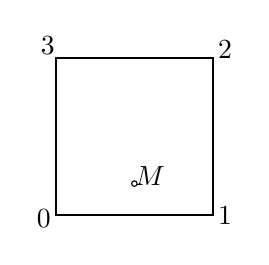
\begin{tikzpicture}
%\draw[step=0.5cm,gray,very thin] (0,0) grid (4,4); %background grid
\draw[thick] (1,1) -- (3,1) -- (3,3) -- (1,3) -- cycle;  
\node[] at (0.85,0.95) {0};
\node[] at (3.15,1) {1};
\node[] at (3.15,3.1) {2};
\node[] at (0.9,3.15) {3};
\node[] at (2.2,1.5) {$M$};
\draw (2.,1.4) circle (1pt);
\end{tikzpicture}\\
\end{center}


%..................................................
\paragraph{An intermediate case} We make the following assumption that the lateral sides of the  
element are vertical while the bottom and top are not necessarily horizontal:

\begin{center}
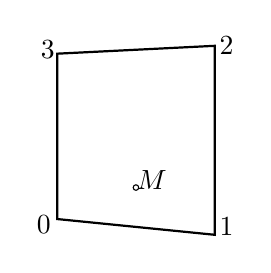
\begin{tikzpicture}
%\draw[step=0.5cm,gray,very thin] (0,0) grid (4,4); %background grid
\draw[thick] (1,1) -- (3,0.8) -- (3,3.2) -- (1,3.1) -- cycle;  
\node[] at (0.83,0.93) {0};
\node[] at (3.15,0.9) {1};
\node[] at (3.15,3.2) {2};
\node[] at (0.88,3.15) {3};
\node[] at (2.2,1.5) {$M$};
\draw (2.,1.4) circle (1pt);
\end{tikzpicture}\\
\end{center}

\noindent Because the sides are verical then if $x_0 \leq x_M \leq x_2$ then 
\[
r_M = \frac{2}{x_2-x_0}(x_M-x_0) -1 
\]
Then, if $M$ is inside the element then its $y$ coordinate is given by
\[
y_M = \sum_i \bN_i(r_M,s_M) y_i
\]
where $\bN_i$ are the four $Q_1$ basis functions associated to the vertices.
Assuming we know $r_M$ then we can solve for $s_M$:
\begin{eqnarray}
y_M &=&  
\frac{1}{4}(1-r_M)(1-s_M) y_0+
\frac{1}{4}(1+r_M)(1-s_M) y_1+
\frac{1}{4}(1+r_M)(1+s_M) y_2+
\frac{1}{4}(1-r_M)(1+s_M) y_3 \nn\\
&=& 
\frac{1}{4} \left[
(1-r)y_0+(1+r)y_1+(1+r)y_2+(1-r)y_3 +s_M [ -(1-r)y_0 - (1+r)y_1+(1+r)y_2+(1-r)y_3  ] 
\right] \nn 
\end{eqnarray}
or, 
\[
s_M = \frac{ 4y_M - [(1-r_M)y_0+(1+r_M)y_1+(1+r_M)y_2+(1-r_M)y_3]  }{ -(1-r_M)y_0 -(1+r_M)y_1+(1+r_M)y_2+(1-r_M)y_3 } 
\]
If the obtained value is in $[-1,1]$ then the point $M$ is in the element.
Verification: when $y_1=y_0$ and $y_2=y_3$ then 
\begin{eqnarray}
s_M 
&=& \frac{4 y_M - [(1-r_M)y_0+(1+r_M)y_0+(1+r_M)y_3+(1-r_M)y_3]  }{ -(1-r_M)y_0 - (1+r_M)y_0+(1+r_M)y_3+(1-r_M)y_3 } \nn\\
&=& \frac{4 y_M - [ 2 y_0 + 2 y_3]  }{ -2 y_0 + 2 y_3    }  \nn\\
&=& \frac{1}{y_3-y_0} [2 y_M - (  y_0 +  y_3) ] \nn\\ 
&=& \frac{1}{y_3-y_0} [2 y_M -  2 y_0 +y_0 -  y_3)  ] \nn\\ 
&=& \frac{2}{y_3-y_0} (y_M - y_0) - 1 
\end{eqnarray}
which is the expression that corresponds to a rectangular element as seen previously.

%..................................................
\paragraph{A generic quadrilateral}

We wish to arrive at a single algorithm which is applicable to all quadrilaterals and we now focus  
on an irregular quadrilateral (no face is parallel to the axis of the coordinate system). 

\begin{center}
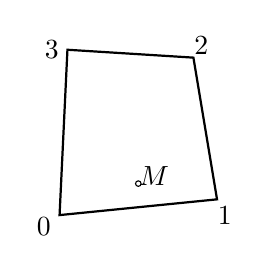
\begin{tikzpicture}
%\draw[step=0.5cm,gray,very thin] (0,0) grid (4,4); %background grid
\draw[thick] (1,1) -- (3,1.2) -- (2.7,3) -- (1.1,3.1) -- cycle;  
\node[] at (0.8,0.85) {0};
\node[] at (3.1,1) {1};
\node[] at (2.8,3.15) {2};
\node[] at (0.9,3.1) {3};
\node[] at (2.2,1.5) {$M$};
\draw (2.,1.4) circle (1pt);
\end{tikzpicture}\\
\end{center}

\noindent Several rather simple options exist:
\begin{itemize}
\item we could subdivide the quadrilateral into two triangles and check whether point $M$ is inside any of them (as it turns out, this problem is rather straightforward for triangles. Simply google it.)
\item We could check that point $M$ is always on the left side of segments $0\rightarrow 1$, $1\rightarrow 2$, $2\rightarrow 3$, $3\rightarrow 0$.
\item ...  
\end{itemize}

Any of these approaches will work although some might be faster than others. 
In three-dimensions all will however become 
cumbersome to implement and might not even work at all. 
Fortunately, there is an elegant way to answer the question, as 
detailed in the following subsection, which works both in 2D and 3D.

%-------------------------------------------
\subsubsection{Three-dimensional space}

If point $M$ is inside the quadrilateral, there exist a set of reduced 
coordinates $r,s,t\in[-1:1]^3$ such that 

\[
\sum_{i=1}^4 \bN_i(r_M,s_M,t_M) x_i = x_M
\quad\quad\quad
\sum_{i=1}^4 \bN_i(r_M,s_M,t_M) y_i = y_M
\quad\quad\quad
\sum_{i=1}^4 \bN_i(r_M,s_M,t_M) z_i = z_M
\]
This can be cast as a system of three equations and three unknowns. 
Unfortunately, each basis function $\bN_i$ 
contains a term $rst$ (as well as $rs$, $rt$, and $st$) 
so that it is not a linear system.
We must then use an iterative technique: the algorithm starts with 
a guess for values $r_M,s_M,t_M$ and 
improves on their value iteration after iteration. 
In what follows the subscript $M$ is dropped from $r,s,t$.

The classical way of solving nonlinear systems of equations is Newton's method. 
\index{general}{Newton's method}
We can rewrite the equations above as ${\bm F}(r,s,t)=0$:
\begin{eqnarray}
\sum_{i=1}^8 \bN_i(r,s,t) x_i - x_M&=&0 \nonumber\\
\sum_{i=1}^8 \bN_i(r,s,t) y_i - y_M&=&0 \nonumber\\
\sum_{i=1}^8 \bN_i(r,s,t) z_i - z_M&=&0
\end{eqnarray}
or,
\begin{eqnarray}
F_r(r,s,t)&=&0 \nonumber\\
F_s(r,s,t)&=&0 \nonumber\\
F_t(r,s,t)&=&0 \nonumber
\end{eqnarray}
so that we now have to find the zeroes of continuously differentiable 
functions ${\bm F}:\mathbb{R} \rightarrow \mathbb{R}$.
The recursion is simply:
\[
\left(
\begin{array}{c}
r_{k+1} \\s_{k+1} \\ t_{k+1}
\end{array}
\right)
=
\left(
\begin{array}{c}
r_{k} \\s_{k} \\ t_{k}
\end{array}
\right)
- J_F(r_k,s_k,t_k) ^{-1} 
\left(
\begin{array}{c}
F_r(r_k,s_k,t_k) \\
F_s(r_k,s_k,t_k)\\
F_t(r_k,s_k,t_k)
\end{array}
\right)
\]
where $J$ the Jacobian matrix:
\begin{eqnarray}
J_F(r_k,s_k,t_k)
&=&
\left(
\begin{array}{ccc}
\frac{\partial F_r}{\partial r}(r_k,s_k,t_k) & \frac{\partial F_r}{\partial s}(r_k,s_k,t_k) & \frac{\partial F_r}{\partial t}(r_k,s_k,t_k) \\\\
\frac{\partial F_s}{\partial r}(r_k,s_k,t_k) & \frac{\partial F_s}{\partial s}(r_k,s_k,t_k) & \frac{\partial F_s}{\partial t}(r_k,s_k,t_k) \\\\
\frac{\partial F_t}{\partial r}(r_k,s_k,t_k) & \frac{\partial F_t}{\partial s}(r_k,s_k,t_k) & \frac{\partial F_t}{\partial t}(r_k,s_k,t_k) 
\end{array}
\right) \nonumber\\
&=&
\left(
\begin{array}{ccc}
\sum\limits_{i=1}^8 \frac{\partial \bN_i}{\partial r}(r_k,s_k,t_k) x_i &
\sum\limits_{i=1}^8 \frac{\partial \bN_i}{\partial s}(r_k,s_k,t_k) x_i &
\sum\limits_{i=1}^8 \frac{\partial \bN_i}{\partial t}(r_k,s_k,t_k) x_i \\
\sum\limits_{i=1}^8 \frac{\partial \bN_i}{\partial r}(r_k,s_k,t_k) y_i &
\sum\limits_{i=1}^8 \frac{\partial \bN_i}{\partial s}(r_k,s_k,t_k) y_i &
\sum\limits_{i=1}^8 \frac{\partial \bN_i}{\partial t}(r_k,s_k,t_k) y_i \\
\sum\limits_{i=1}^8 \frac{\partial \bN_i}{\partial r}(r_k,s_k,t_k) z_i &
\sum\limits_{i=1}^8 \frac{\partial \bN_i}{\partial s}(r_k,s_k,t_k) z_i &
\sum\limits_{i=1}^8 \frac{\partial \bN_i}{\partial t}(r_k,s_k,t_k) z_i 
\end{array}
\right) \nonumber 
\end{eqnarray}
In practice, we solve the following system:
\[
J_F(r_k,s_k,t_k) 
\left[  
\left(
\begin{array}{c}
r_{k+1} \\s_{k+1} \\ t_{k+1}
\end{array}
\right)
-
\left(
\begin{array}{c}
r_{k} \\s_{k} \\ t_{k}
\end{array}
\right)
\right]=-
\left(
\begin{array}{c}
F_r(r_k,s_k,t_k) \\
F_s(r_k,s_k,t_k)\\
F_t(r_k,s_k,t_k)
\end{array}
\right)
\]
Finally, the algorithm goes as follows:
\begin{itemize}
\item set guess values for $r,s,t$ (typically 0)
\item loop over k=0,...
\item Compute rhs= $-{\bm F}(r_k,s_k,t_k)$ 
\item Compute matrix $J_F(r_k,s_k,t_k)$
\item solve system for $(dr_k,ds_k,dt_k)$
\item update $r_{k+1}=r_k+dr_k$, $s_{k+1}=s_k+ds_k$, $t_{k+1}=t_k+dt_k$ 
\item stop iterations when $(dr_k,ds_k,dt_k)$ is small
\item if $r_k,s_k,t_k\in[-1,1]^3$ then $M$ is inside.
\end{itemize}
This method converges quickly but involves iterations, and multiple 
solves of $3\times 3$ systems which, when carried out for each marker 
and at each time step can prove to be expensive. 
A simple modification can be added to the above algorithm: 
iterations should be carried out {\it only}
when the point $M$ is inside of a cuboid of 
size $[\min\limits_i{x_i}:\max\limits_i{x_i}]\times[\min\limits_i{y_i}:\max\limits_i{y_i} ]
\times[\min\limits_i{z_i}:\max\limits_i{z_i}]$ where the sums run over the vertices of the element. 
In 2D this translates as follows: only carry out Newton iterations when $M$ is inside the red rectangle!
\begin{center}
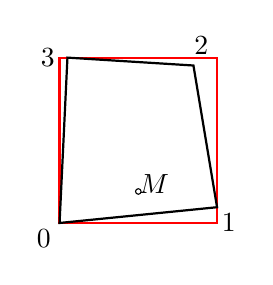
\begin{tikzpicture}
%\draw[step=0.5cm,gray,very thin] (0,0) grid (4,4); %background grid
\draw[thick,red] (1,1) -- (3,1) -- (3,3.1) -- (1,3.1) -- cycle;  
\draw[thick] (1,1) -- (3,1.2) -- (2.7,3) -- (1.1,3.1) -- cycle;  
\node[] at (0.8,0.8) {0};
\node[] at (3.15,1) {1};
\node[] at (2.8,3.25) {2};
\node[] at (0.85,3.1) {3};
\node[] at (2.2,1.5) {$M$};
\draw (2.,1.4) circle (1pt);
\end{tikzpicture}\\
\end{center}

Note that the algorithm above extends to high degree elements 
such as $Q_2$ and higher, even with curved sides.
As shown in the 2D case if the element is a cuboid or 
if all its lateral faces are vertical then one can 
compute the reduced coordinates without using an iterative method.


%-----------------------------------------------------
\subsubsection{Three-dimensional space - special case}

We assume that the mesh is such that the cross section of all $Q_1$ elements 
is a rectangle in the $xy$-plane. 

Let $(x,y,z)$ be a point inside the element. 
The global coordinates $x,y,z$ are obtained from the 
reduced coordinates $r,s,t$ via the basis the basis functions:
\begin{eqnarray}
x=\sum_{i=1}^8 \bN_i (r,s,t) x_i \qquad 
y=\sum_{i=1}^8 \bN_i (r,s,t) y_i  \qquad 
z=\sum_{i=1}^8 \bN_i (r,s,t) z_i \label{xyz}
\end{eqnarray}
Let 
\begin{eqnarray}
{\vec v}_1 &=& (+1,+1,+1,+1,+1,+1,+1,+1) \nn\\
{\vec v}_2 &=& (-1,+1,+1,-1,-1,+1,+1,-1) \nn\\
{\vec v}_3 &=& (-1,-1,+1,+1,-1,-1,+1,+1) \nn\\
{\vec v}_4 &=& (-1,-1,-1,-1,+1,+1,+1,+1) \nn\\
{\vec v}_5 &=& (+1,-1,+1,-1,+1,-1,+1,-1) \nn\\
{\vec v}_6 &=& (+1,-1,-1,+1,-1,+1,+1,-1) \nn\\
{\vec v}_7 &=& (+1,+1,-1,-1,-1,-1,+1,+1) \nn
\end{eqnarray}
and 
\begin{eqnarray}
{\vec x} &=& (x_1,x_2,x_3,x_4,x_5,x_6,x_7,x_8) \nn\\
{\vec y} &=& (y_1,y_2,y_3,y_4,y_5,y_6,y_7,y_8) \nn\\
{\vec z} &=& (z_1,z_2,z_3,z_4,z_5,z_6,z_7,z_8) \nn
\end{eqnarray}
then Eqs.~\eqref{xyz} can also be written
\begin{eqnarray}
x&=&\frac{1}{8} \left( {\vec v}_1 + r  {\vec v}_2 + s  {\vec v}_3 + t  {\vec v}_4 
                 + rs  {\vec v}_5 + rt {\vec v}_6 + st {\vec v}_7 \right) \cdot {\vec x} \nn\\ 
y&=&\frac{1}{8} \left( {\vec v}_1 + r  {\vec v}_2 + s  {\vec v}_3 + t  {\vec v}_4 
                 + rs  {\vec v}_5 + rt {\vec v}_6 + st {\vec v}_7 \right) \cdot {\vec y} \nn\\
z&=&\frac{1}{8} \left( {\vec v}_1 + r  {\vec v}_2 + s  {\vec v}_3 + t  {\vec v}_4 
                 + rs  {\vec v}_5 + rt {\vec v}_6 + st {\vec v}_7 \right) \cdot {\vec z} \label{zzz}
\end{eqnarray}
If the element has a rectangular cross-section $s_x \times s_y$ then 
\begin{eqnarray}
{\vec x} &=& (x_0,x_0+s_x,x_0+s_x,x_0,x_0,x_0+s_x,x_0+s_x,x_0) \nn\\
{\vec y} &=& (y_0,y_0,y_0+s_y,y_0+s_y,y_0,y_0,y_0+s_y,y_0+s_y) \nn
\end{eqnarray}
which yields
\begin{eqnarray}
r&=& 2\frac{x-x_0}{s_x}-1  \nn\\
s&=& 2\frac{y-y_0}{s_y}-1  \nn
\end{eqnarray}
Since the local coordinates $r$ and $s$ can be easily computed, one can use Eq.~\eqref{zzz} to obtain $t$:
\[
t=\frac{8z - ({\vec v}_1 + r {\vec v}_2 + s {\vec v}_3 + rs  {\vec v}_5 ) \cdot {\vec z}} 
{ ({\vec v}_4  + r  {\vec v}_6 + s  {\vec v}_7)  \cdot {\vec z} }
\]







 
 %----------------------------------
\newpage %-----------------------------------------------------------------------------------------
\section{Static condensation} \input{static_condensation} %----------------------------------------
\newpage %-----------------------------------------------------------------------------------------
\section{Measuring incompressibility \label{ss_incomp}} 
The velocity divergence error integrated over the whole element is given by
\begin{equation}
e_{div}= \int_\Omega (\vec\nabla\cdot \vec v^h - \underbrace{\vec\nabla\cdot \vec v}_{=0}  ) \; d\Omega
= \int_\Omega (\vec\nabla\cdot \vec v^h) \; d\Omega
\end{equation}
where $\Gamma_e$ is the boundary of element $e$ and $\vec{n}$ is the unit 
outward normal of $\Gamma_e$.

Furthermore, one can show that \cite{dobo04}:
\[
e_{div} = \int_{\Gamma_e} \vec{v}^h\cdot\vec{n} \;  d\Gamma
\]
The reason is as follows and is called the divergence 
theorem\footnote{\url{https://en.wikipedia.org/wiki/Divergence_theorem}}:
suppose a volume $V$ subset of $\mathbb{R}^d$ which is compact
and has a piecewise smooth boundary $S$, and if $\vec F$ is
a continuously differentiable vector field then
\[
\int_V ( \vec\nabla\cdot\vec F)\; dV = \int_S (\vec F \cdot \vec n)\; dS
\]
The left side is a volume integral while the right side is a surface integral.
Note that sometimes the notation $d\vec S = \vec n \; dS $ is used so that 
$\vec F \cdot \vec n \; dS = \vec F \cdot d\vec S$.

The average velocity divergence over an element can be defined as 
\[
<\vec \nabla \cdot \vec v>_e 
= \frac{1}{V_e} \int_{\Omega_e}  (\vec\nabla\cdot\vec v) \; d\Omega
= \frac{1}{V_e} \int_{\Gamma_e} \vec{v}\cdot\vec{n} \; d\Gamma
\]
Note that for elements using discontinuous pressures we shall 
recover a zero divergence element per element (local mass conservation)
while for continuous pressure elements the mass conservation 
is guaranteed only globally (i.e. over the whole domain), see section 3.13.2 of \cite{grsa}.

Note that one could instead compute $<|\vec\nabla\cdot \vec v|>_e$. Either volume or 
surface integral can be computed by means of an appropriate Gauss-Legendre quadrature algorithm.



 %---------------------------
\newpage %-----------------------------------------------------------------------------------------
\section{Picard and Newton \label{ss_nonlinear}} \index{general}{Nonlinear PDE} 
\index{general}{Picard Iterations} 
\index{general}{Relaxation}

\todo[inline]{explain why our eqs are nonlinear}

\Literature Quasi Newton methods \cite{ensb81}

%--------------------------------
\subsubsection{Picard iterations} \label{ss:picard}

Let us consider the following system of nonlinear algebraic equations:
\[
\mathbb{A}(\vec X) \cdot \vec X = \vec b(\vec X)
\]
Both matrix and right hand side depend on the solution vector $\vec X$.

For many mildly nonlinear problems, a simple successive substitution 
iteration scheme (also called Picard method) will converge to the solution
and it is given by the simple relationship:
\[
\mathbb{A}(\vec X^n) \cdot \vec X^{n+1} = \vec b(\vec X^n)
\]
where $n$ is the iteration number. 
It is easy to implement:
\begin{enumerate}
\item guess $\vec X^0$ or use the solution from previous time step
\item compute $\mathbb{A}$ and $\vec b$ with current solution vector $\vec X^{old}$
\item solve system, obtain $T^{new}$
\item check for convergence (are $\vec X^{old}$ and $\vec X^{new}$ close enough?)
\item $\vec X^{old} \leftarrow \vec X^{new}$
\item go back to 2.
\end{enumerate}

There are various ways to test whether iterations have converged. The simplest
one is to look at $\norm{\vec X^{old}-\vec X^{new} }$ (in the $L_1$, $L_2$ or maximum norm)
and assess whether this term is smaller than a given tolerance $\epsilon$. 
However this approach poses a problem: in geodynamics, if two consecutively obtained 
temperatures do not change by more than a thousandth of a Kelvin (say $\epsilon=10^{-3}$K )
we could consider that iterations have converged but looking now at velocities which 
are of the order of a cm/year (i.e. $\sim 3\cdot 10^{-11}$m/s) we would need a tolerance 
probably less than $10^{-13}$m/s. We see that using absolute values for a convergence 
criterion is a potentially dangerous affair, which is why one uses a relative 
formulation (thereby making $\epsilon$ a dimensionless parameter):
\[
\frac{\norm{\vec X^{old}-\vec X^{new}}}{\norm{\vec X^{new}}} < \epsilon
\]
Another convergence criterion is proposed by Reddy (section 3.7.2) \cite{reddybook2}:
\[
\left(
\frac{ (\vec X^{old}-\vec X^{new})\cdot(\vec X^{old}-\vec X^{new} ) }{ X^{new}\cdot X^{new}  } 
\right)^{1/2} < \epsilon
\]
Yet another convergence criterion is used in \cite{thie11}: the means $<\vec X^{old}>$, $<\vec X^{new}>$
as well as the variances $\sigma^{old}$ and $\sigma^{new}$ are computed, followed by the 
correlation factor $R$:
\[
R= \frac{ <  (\vec X^{old}-<\vec X^{old}>)\cdot( \vec X^{new}-<\vec X^{new}> )>  }{\sqrt{\sigma^{old}\sigma^{new}}}
\]
Since the correlation is normalised, it takes values between 0
(very dissimilar velocity fields) and 1 (very similar fields). The
following convergence criterion is then used: $1-R < \epsilon$.

\todo[inline]{write about nonlinear residual}


Note that in some instances and improvement in convergence rate can be obtained by use of a 
relaxation formula where one first solves
\[
\mathbb{A}(\vec X^n) \cdot \vec X^{\star} = \vec b(\vec X^n)
\]
and then updates $\vec X^n$ as follows:
\[
\vec X^n = \gamma \vec X^n + (1-\gamma) \vec X^\star 
\quad\quad\quad
0 < \gamma \leq 1
\]
When $\gamma=1$ we recover the standard Picard iterations formula above.

%------------------------------------------
\subsection{Defect correction formulation}
\index{general}{Defect Correction Formulation}

Work in progress. 

We start from the system to solve:
\[
{\bm A}(\vec X) \cdot \vec X = \vec b(\vec X)
\]
with the associated residual vector $\vec F$ 
\[
\vec F(\vec X) = {\bm A}(\vec X) \cdot \vec X - \vec b(\vec X)
\]
The Newton-Raphson algorithm consists of two steps:
\begin{enumerate}
\item solve $\bm J_k \cdot \delta \vec X_k = -\vec F(\vec X_k)$, or in the 
case of the incompressible Stokes equation FEM system:
\[
\left(
\begin{array}{cc}
\bm J^{{\cal V}{\cal V}}_k & \bm J^{{\cal V}{\cal P}}_k \\
\bm J^{{\cal P}{\cal V}}_k & 0
\end{array}
\right)
\cdot
\left(
\begin{array}{c}
\delta \vec {\cal V}_k \\ \delta \vec {\cal P}_k
\end{array}
\right)
=
\left(
\begin{array}{c}
- \vec F_k^{\cal V} \\ -\vec F_k^{\cal P}
\end{array}
\right)
\]

\item update $\vec X_{k+1} = \vec X_k + \alpha_k \delta \vec X_k$
\end{enumerate}
The defect correction Picard approach consists of neglecting the derivative terms present 
in the $J$ terms (Eqs. 16,17,18 of \cite{frbt19}) so that 
\[
\bm J^{{\cal V}{\cal V}}_k \simeq \K_k 
\quad\quad
\bm J^{{\cal V}{\cal P}}_k \simeq \G 
\quad\quad
\bm J^{{\cal P}{\cal V}}_k \simeq \G^T
\]
and step 1 of the above iterations become:
\[
\left(
\begin{array}{cc}
\K_k & \G \\ \G^T & 0
\end{array}
\right)
\cdot
\left(
\begin{array}{c}
\delta \vec {\cal V}_k \\ \delta \vec {\cal P}_k
\end{array}
\right)
=
\left(
\begin{array}{c}
- \vec F_k^{\cal V} \\ -\vec F_k^{\cal P}
\end{array}
\right)
\]


\mscthesis: implement a simple Newton solver and apply it to a few nonlinear 
benchmarks. \index{general}{MSc Thesis} 

\vspace{1cm}

\todo[inline]{explain picard, defect picard, Newton, line search, ....}


\begin{itemize}
\item \fullcite{erka81}
\item \fullcite{ensb81}
\item \fullcite{knke04}
\item \fullcite{yiha10}
\item \fullcite{sara16}
\item \fullcite{frbt19}
\item \fullcite{russ20}
\end{itemize}

 %----------------------------
\newpage %-----------------------------------------------------------------------------------------
\section{Parallel or not?} \label{sec:parallel} \input{parallel} %------------------------------
\newpage %-----------------------------------------------------------------------------------------
\section{Stream function} \label{sec:streamfunction} \index{general}{Stream Function}
\begin{flushright} {\tiny {\color{gray} streamfunction.tex}} \end{flushright}

\Literature 
\textcite{scja81} (1981),
\textcite{chyu84} (1984),
\textcite{chri84} (1984),
\textcite{hayu94} (1994),
\textcite{olwh97} (1997),
\textcite{giju98} (1998),
\textcite{vanv08} (2008),
\textcite{vanj11} (2011).

\vspace{0.5cm}

The Stream function (commonly denoted by $\Phi$ or $\Psi$) approach is a useful approach in 
fluid dynamics as it 
can provide relatively quick solutions to 2D incompressible flow problems.
Using a stream function
formulation is numerically convenient because velocity information is contained in a single scalar equation
and pressure vanishes from the solution process.
The stream function is a function of coordinates and time of an inviscid liquid.
It allows to determine the components of velocity by differentiating the stream function 
with respect to the space coordinates. 
A family of curves $\Psi = constant$ represent {\color{olive} streamlines}, i.e. 
the stream function remains constant along a streamline. 
Although also valid in 3D, this approach is mostly used in 2D because of its 
relative simplicity.

%............................................
\subsubsection{In Cartesian coordinates - 2D}

In two dimensions the velocity is obtained as follows:
\begin{equation}
{\vec \upnu} = (u,v) = \left( \frac{\partial \Psi}{\partial y},-\frac{\partial \Psi}{\partial x} \right) 
\end{equation}
Provided the function $\Psi$ is a smooth enough function, 
this automatically insures that the flow is incompressible:
\begin{equation}
{\vec \nabla}\cdot {\vec \upnu} = 
\frac{\partial u}{\partial x} + \frac{\partial v}{\partial y}
=
\frac{\partial^2 \Psi}{\partial xy} - \frac{\partial^2 \Psi}{\partial xy} =0 
\end{equation}
Assuming constant viscosity, the Stokes equation writes:
\begin{equation}
-{\vec \nabla}p + \eta \Delta {\vec \upnu} + \rho {\vec g} = \vec{0}
\end{equation}
Let us introduce the vector $\vec{W}=(W_x,W_y)$ for convenience such that in each dimension:
\begin{eqnarray}
W_x&=&-\frac{\partial p}{\partial x} 
+ \eta\left( \frac{\partial^2 u}{\partial x^2} + \frac{\partial^2 u}{\partial x^y} \right) \\
W_y&=&-\frac{\partial p}{\partial y} 
+ \eta \left(\frac{\partial^2 v}{\partial x^2} + \frac{\partial^2 v}{\partial x^y} \right) 
\end{eqnarray}
Taking the curl of the vector ${\vec{W}}$ and only considering the component 
perpendicular to the $xy$-plane:
\begin{equation}
\frac{\partial W_y}{\partial x} - \frac{\partial W_x}{\partial y}  = 
-\frac{\partial \rho g_y}{\partial x} + \frac{\partial \rho g_x}{\partial y}   
\end{equation}
The advantage of this approach is that the pressure terms cancel out 
(the curl of a gradient is always zero\footnote{\url{https://mathinsight.org/curl_gradient_zero}}), 
so that:
\begin{equation}
\frac{\partial}{\partial x}\eta\left( \frac{\partial^2 v}{\partial x^2} + \frac{\partial^2 v}{\partial x^y}  \right) 
- \frac{\partial }{\partial y} \eta \left( \frac{\partial^2 u}{\partial x^2} + \frac{\partial^2 u}{\partial x^y} \right) = 
-\frac{\partial \rho g_y}{\partial x} + \frac{\partial \rho g_x}{\partial y}   
\end{equation}
and then replacing $u,v$ by the their stream function derivatives yields (for a constant viscosity):
\begin{equation}
\eta \left(\frac{\partial^4 \Psi}{\partial x^4} + 
\frac{\partial^4 \Psi}{\partial y^4} + 
2\frac{\partial^4 \Psi}{\partial x^2y^2} \right)
=
-\frac{\partial \rho g_y}{\partial x} + \frac{\partial \rho g_x}{\partial y}   
\end{equation}
or, 
\begin{equation}
\eta {\vec \nabla}^4 \Psi 
=
\left(\frac{\partial^2 }{\partial x^2} + \frac{\partial^2 }{\partial y^2} \right) 
\left(\frac{\partial^2 }{\partial x^2} + \frac{\partial^2 }{\partial y^2} \right) \Psi
=
-\frac{\partial \rho g_y}{\partial x} + \frac{\partial \rho g_x}{\partial y}   
\label{eq:sf1}
\end{equation}
Note that $\vec\nabla^2 \vec\nabla^2 = \vec\nabla^4 $ is known as the {\color{olive}Biharmonic operator}.
\index{general}{Biharmonic Operator} 
These equations are also to be found in the geodynamics literature, 
see \textcite[eq. 1.43]{tack10} or \textcite[p 70-71]{gery10}.

In the presence of temperature variations and multiple compositions, 
\textcite{trlb20} (2020)  use the  following nondimensional equation:
\[
\left(
\frac{\partial^2 }{\partial x^2} - 
\frac{\partial^2 }{\partial y^2}  
\right)
\left[ \eta
\left(
\frac{\partial^2 \Psi}{\partial x^2} - 
\frac{\partial^2 \Psi}{\partial y^2}  
\right)
\right]
+4
\frac{\partial^2 }{\partial xy} 
\left[
\eta 
\frac{\partial^2 \Psi}{\partial xy} 
\right]
=
Ra_T \frac{\partial T}{\partial x}-
Ra_C \frac{\partial C}{\partial x}
\]
\todo[inline]{check/rederive this formula!}

%........................................
%\subsubsection{In Cylindrical coordinates}

%TODO

%VERIFY THOSE! minus signs ?
%\[
%\upnu_r=\frac{1}{r}\frac{\partial \Phi}{\partial \theta} 
%\]
%\[
%\upnu_\theta=-\frac{\partial \Phi}{\partial r} 
%\]


%............................................
\subsubsection{In Cartesian coordinates - 3D}

See for example \textcite{hous90} (1990) and refs therein.


 %-------------------
\newpage %-----------------------------------------------------------------------------------------
\section{Corner flow} \label{sec:cornerflow} \input{cornerflow} %-------------------------------
\newpage %-----------------------------------------------------------------------------------------
\section{Surface processes \label{sec:surfaceprocesses}} \begin{flushright} {\tiny {\color{gray} surfaceprocesses.tex}} \end{flushright}

%.......................................................................
\subsubsection{In 1D - simple nonlinear diffusion a la Burov \& Cloetingh (1997)}

This approach comes from \textcite{bucl97} (1997).
The tectonic-scale transport equations describe long term changes
in topography $h(x,y,t)$ as a result of simultaneous short- and long-range
mass transport processes \cite{befh92,kobe94}.

The short-range surface processes are represented by cumulative effects of hillslope 
processes (soil creep, rainsplash, slides) that remove material from uplifted areas 
down to the valleys. 
It is then assumed that the horizontal material flux $\vec{q}_s$ is related to 
local slope $\vec\nabla h$ by $\vec{q}_s=-K_s \vec{\nabla}h$ 
where $K_s$ is the effective diffusivity. Assumption of conservation of mass 
volume leads to the linear diffusion equation for erosion:
\[
\frac{\partial h}{\partial t} = K_s \Delta h
\]
This equation can be solved with constant-elevation (fixed $h$ value)
boundary conditions simulating local base levels of erosion. 

Note that is practice the coefficient $K_s$ might depend on slope and curvature, 
i.e.
\[
\frac{\partial h}{\partial t} = K_s(x,y,h,\vec\nabla h)\Delta h
\]
Following \cite{goss76}, Burov \& Cloetingh use an empirical non linear 
expression $K_s=k_s(x) (\vec\nabla h)^n$. 




%...........................................................
\subsubsection{In 1D - not so simple, a la Andr\`es-Martinez \etal (2019)}

This approach comes from \textcite{anpa19} (2019). 
The change in surface elevation rate due to surface processes is equal
to the divergence of the sediment flux 
(assuming there is no density difference between the bedrock and
sediment and ignoring the effects of compaction):
\[
\frac{\partial h}{\partial t} = -\frac{\partial q_s}{\partial x}
\]
where $h$ is the topography, $t$ is the time, $q_s$ represents the sediment flux, 
and $x$ is the horizontal coordinate. 

The next step consists in a formulation for the sediment flux. Still following \cite{anpa19}, 
in the subaerial environment, it is possible to define the sediment transport 
flux $q_s$ in terms of the water flux $q_w$ as
\[
q_s=-(K+c q_w^n) \frac{\partial h}{\partial x}
\]
where $K$ is the slope diffusivity, $c$ is the transport coefficient, 
and $n \geq 1$ is the power law that defines the type
of relationship between the sediment transport and the water flux 
(Simpson \& Schlunegger, 2003; Smith \& Bretherton, 1972).
\todo[inline]{get these papers}
This model accounts for hillslope diffusion processes where the topography will tend to
a dispersive diffusion (Culling, 1960) and fluvial transport processes that result in concentrative diffusion
due to water run off (Graf, 1984). For a simple parameterization we choose a linear relationship between
sediment transport and water flux $(n=1)$.

The water flux can be related to the water discharge/effective rainfall $\alpha$ as
\[
\frac{\partial}{\partial x} (\vec{n} q_w) = -\alpha
\]
where $\vec n$ is a unit vector directed down the surface gradient (Smith \& Bretherton, 1972). 
By assuming a constant $\alpha$ and integrating equation (12) over the surface in the downstream direction, we obtain

\[
q_w = \alpha x_d
\]
where $x_d$ is the downstream distance from the drainage divide. By substituting equations (11) and
(13) into (10) we obtain the 1-D sediment mass conservation equation for combined hillslope and
discharge-dependent fluvial transport
\[
\frac{\partial h}{\partial t} = \frac{\partial}{\partial x} \left( (K+k \alpha x_d) 
\frac{\partial h}{\partial x}   \right)
\]
where the downstream distance $x_d$ is calculated at each time step as the distance from the topographic highs
to the valley floors. Because $q_w$ is dependent on the length of the drainage, the model mimics 1-D landscapes
similar to river profiles in which fluvial processes are dominant.

%...........................................................
\subsubsection{Examples in the literature}

\begin{center}
\includegraphics[width=7cm]{images/surfaceprocesses/fuwf06a}
\includegraphics[width=7cm]{images/surfaceprocesses/fuwf06b}\\
{\captionfont Application to Taiwan. Taken from Fuller \etal (2006) \cite{fuwf06}}
\end{center}


 %-------------
\newpage %-----------------------------------------------------------------------------------------
\section{Geometric multigrid} \input{gmg} %-----------------------------------------------------
\newpage %-----------------------------------------------------------------------------------------
\section{Algebraic multigrid} \input{amg} %-----------------------------------------------------
\newpage %-----------------------------------------------------------------------------------------
\section{Computing depth \label{ss:depth}} \input{computing_depth} %----------------------------
\newpage %-----------------------------------------------------------------------------------------
\section{The Geoid} \label{ss:geoid} 
%---------------------------------
\subsubsection{What is the geoid?}
\index{general}{Geoid}


There is an infinity of equipotential surfaces of the gravitational potential $U$.
However, there is a particular surface on the Earth that is "easy" to locate: 
the mean sea level. This is a somewhat arbitrary choice  
but it makes sense because the oceans are made of water (!): 
the surface of a fluid in equilibrium must follow an equipotential.

\begin{center}
\includegraphics[width=6cm]{images/geoid/geoid1}
\end{center}

The geoid is usually defined in two ways:
\begin{itemize}
\item it is the particular equipotential surface that coincides with the mean sea level
 (easy to define in the oceans -assuming no currents, waves,... - but harder on land since 
it is not the topographic surface).
\item A gravitational equipotential surface. This means that everywhere at sea level experiences the same value of gravity potential, so there is no tendency for water to flow downhill since all points in the vicinity have the same value of gravity potential, pointed toward the center of the earth.
\end{itemize}

\begin{center}
\includegraphics[width=13cm]{images/geoid/ww15mgh}\\
{\captionfont Data Max value: 85.4 meters, east of New Guinea. Data Min value:-107.0 meters, south of India. 
This image shows 15'x15' geoid undulations covering the planet Earth 
from the NIMA/GSFC WGS-84 EGM96 15' Geoid Height File. The undulations refer to 
the differences from the WGS-84(G873) reference ellipsoid. 
Map and description from National Geodetic Survey
\footnote{\url{https://www.usna.edu/Users/oceano/pguth/md_help/geology_course/geoid.htm}}
}
\end{center}

From Wikipedia: The geoid surface is irregular, unlike the reference ellipsoid 
(which is a mathematical idealized representation of the physical Earth), but 
is considerably smoother than Earth's physical surface. Although the physical Earth has 
excursions of +8,848 m (Mount Everest) and -11,034 m (Marianas Trench), 
the geoid's deviation from an ellipsoid ranges from +85 m (Iceland) to -106 m (southern India), 
less than 200 \si{metre} total.


\begin{center}
\includegraphics[width=8cm]{images/geoid/Geoid}\\
{\captionfont 1. Ocean
2. Reference ellipsoid
3. Local plumb line
4. Continent
5. Geoid\\
Taken from \url{https://en.wikipedia.org/wiki/Geoid}}
\end{center}


%----------------------------------------
\subsubsection{the (reference) ellipsoid}

First evidence that the Earth is round Erathostene (275-195 B.C.)

First hypothesis that the Earth is flattened at the poles: Newton

First measurement of the Earth's flattening at the poles: Clairaut (1736) and Bouguer (1743)

The shape of the Earth can be mathematically represented as an ellipsoid defined by:
\begin{itemize}
\item Semi-major axis = equatorial radius = $a$
\item Semi-minor axis = polar radius = $c$
\item Flattening (the relationship between equatorial and polar radius): $f = (a-c)/a$
\item Eccentricity: $e^2 =2f-f^2$
\end{itemize}

Many different reference ellipsoids have been defined and are in use.
We define the {\it reference ellipsoid} = the ellipsoid that best fits the geoid.
It is totally arbitrary, but practical. 
The most common reference ellipsoid is the WGS-84 one\footnote{\url{https://confluence.qps.nl/qinsy/latest/en/world-geodetic-system-1984-wgs84-182618391.html}}:

\begin{center}
\includegraphics[width=6cm]{images/geoid/ellipsoid_wgs84}\\
Taken from \url{https://en.wikipedia.org/wiki/Reference_ellipsoid}
\end{center}


Geoid undulations = differences, in meters, between
the geoid reference ellipsoid
(= geoid ``height'').

To clarify:
\begin{itemize}
\item Geoid = the equipotential surface of the Earth's gravity field that
best fits (in a least squares sense) the mean sea level.
The gravitational potential is constant on the geoid (by definition) but 
the gravitational acceleration is not! 

\item Reference Ellipsoid = the ellipsoid that best fits the geoid 
\item Geoid = the (actual) figure of the Earth 
\item Ellipsoid = the (theoretical) shape of the Earth
\end{itemize}



%---------------------------------
\subsubsection{How to compute it?}

From \textcite{lizh16} (2016): ``
The geoid is computed by $\phi/g$, where $\phi$ is the surface gravitational potential anomaly 
and can be solved from the Poisson equation,
$ \nabla^2 \phi = -4\pi {\cal G} \delta\rho$ 
where ${\cal G}$ is the gravitational constant, and $\delta\rho$ 
includes both density variations in the mantle [...]
and those associated with dynamic topographies at the surface and CMB. 
Dynamic topographies are determined from solving [the Stokes] equations 
under free-slip boundary conditions at the surface and CMB.''


%---------------------------------
\subsubsection{Interesting modelling}

\begin{center}
\includegraphics[width=15cm]{images/geoid/mogu96}
{\scriptsize Idealized 2D slab calculations for each viscosity model: geoid and geoid filtered 
to pass only the longest wavelengths ($\sim$ 4000 km).
(a) Cold slab extends to 500 km depth in the upper mantle, 
(b) Slab extends to 750 km so that it is partly supported by the high viscosity lower mantle at 670 km. 
(c) Slab tilted at 45\degree to the vertical extending to the top of the lower mantle. 
Taken from \cite{mogu96}}
\end{center}
 %-----------------------------------------------
\newpage %-----------------------------------------------------------------------------------------
\section{The Lyapunov time/exponent, mixing stirring}\label{ss:lyapunov}\index{general}{Lyapunov Time}
\begin{flushright} {\tiny {\color{gray} lyapunov.tex}} \end{flushright}

%from wiki

Simply put, the Lyapunov time is the characteristic timescale on which a dynamical system is chaotic.
 It is defined as the inverse of a system's largest Lyapunov exponent.

The Lyapunov time mirrors the limits of the predictability of the system. By convention, it is defined 
as the time for the distance between nearby trajectories of the system to increase by a factor of $e$. 
However, measures in terms of 2-foldings and 10-foldings are sometimes found, since they correspond to 
the loss of one bit of information or one digit of precision respectively.

The Lyapunov exponent or Lyapunov characteristic exponent of a dynamical system is a quantity 
that characterizes the rate of separation of infinitesimally close trajectories. 
Quantitatively, two trajectories in phase space with initial separation $\delta \mathbf{Z}_0$ 
diverge (provided that the divergence can be treated within the linearized approximation) at a rate given by
\[
|\delta \mathbf{Z} (t)|\approx e^{\lambda t}|\delta \mathbf {Z} _{0}| 
\]
where $\lambda$ is the Lyapunov exponent. 

Measuring the Lyapunov exponent or time (or related quantities) is relevant in the context of mantle stirring. 
On the one hand it is argued that the mantle is convecting and very efficient at mixing resulting in a 
somewhat homogenous composition. On the other hand, there is are modeling studies that suggest that
whole-mantle convection can preserve heterogeneity in the presence of well-mixed mantle. 

%from vazh99
Mixing takes place by the repeated stretching
and folding of interfaces. A measure of the
mixing efficiency is the time evolution of the area of
the mixing surface. Maximum efficiency of mixing
is reached with turbulent mixing behavior where
One can formally show whether mixing is laminar or turbulent by evaluating the Luyaponov exponents $\sigma$ .
These are of the form:
\[
\sigma = \lim_{t\rightarrow \infty} \lim_{X\rightarrow 0} \left[  \frac{1}{t} \ln \left( \frac{X(t)}{X(t=0)} \right)   \right]
\]
where $X(t)$ is the length of this segment at time t.
Non-zero Luyaponov exponents indicate that
stretching is exponential and the larger the exponent,
the more efficient mixing is.
However, the limits in the above equation are difficult to evaluate and the interpretation 
of the 'finite-time' Luyaponov exponent, where both limits are truncated, is difficult to formalize.


Two approaches are taken in the literature when it comes to studying mixing/stirring and/or measuring Lyapunov quantities::

\begin{itemize}
\item using marker advection: in \textcite{vazh99} (1999) the authors use a steady state velocity
pattern obtained for a model of present-day mantle convection. The velocity model is
based on the solution of the Stokes equations in a 3D spherical model with variable rheology.
To study mixing, they release particles in the velocity model and follow 
these by numerical integration. 

\begin{center}
\includegraphics[width=6cm]{images/mixing/vazh99}\\
{\captionfont a) The three particles in this plot were
selected for their relatively regular pattern. 
b) Three other particles that traverse a large portion of the model. These particles feel 
the strong toroidal motion and their paths form corkscrew-like patterns. 
They indicate that certain parts of the model can exhibit strong mixing. 
Taken from \textcite{vazh99} (1999).}
\end{center}

Rather than calculating the exponents explicitly, the authors 
use an approximation to the finite-time,
finite-length Luyaponov exponent by evaluating the distance between two points that are closely spaced
at time $t=0$. For this they compute the advection of a
large number of 10 km long line segments that were
originally at 1500 km depth. The length of these segments is approximated by the distance between the
endpoints and the results are summarized in the following figure:

\begin{center}
\includegraphics[width=7cm]{images/mixing/vazh99b}\\
{\captionfont Length
of the line segment after 4 billion years. Approximately 14,000 line segments were released with 
regular spacing at 1500 km depth. The length of the segment is indicated by the colored symbols 
that are plotted at the initial position. The results indicate that there is a strong
diversity in mixing behavior. In some regions (north Pacific, parts under the Indian/Australian plate) 
stretching is very limited, indicating laminar and consequently inefficient mixing. Regions that 
are under strong toroidal surface motion (western Pacific, Nazca and South
America) show very efficient stretching of up to the maximum length of the diameter of the Earth. 
Taken from \textcite{vazh99} (1999).}
\end{center}


\item twin experiments: \fullcite{becr14} (2014)
\end{itemize}

Talk about configurational entropy \fullcite{gobo02},\fullcite{nake07} (2007), van der Wiel et al.
\fullcite{cakm06} 

Talk about retrodiction (reconstructions of past states of Earth's mantle obtained using present information)
\textcite{cobs15} (2015),
\textcite{cogb18} (2018).

\Literature: 
\textcite{scha94} (1994),
\textcite{schh96} (1996),
\textcite{vazh99} (1999),
\textcite{falt02} (2002),

\textcite{fasa03} (2003),
\textcite{saad11} (2011),

\textcite{sato12} (2012) measure the convective stirring efficiency using two Lagrangian methods: 
the first determines the mixing time associated with
different wavelengths of heterogeneity following the approach of
Ferrachat and Ricard (2001). The second determines the value of
the maximum Finite Time Lyapunov Exponents (FTLE) as de-
scribed in Farnetani and Samuel (2003), and measures the rate at
which heterogeneities are stretched by mantle motions.

Investigating the initial condition
of mantle models using data assimilation. PhD thesis. \textcite{pric16} (2016).

Reconstruction of mantle convection and surface tectonics with (ensemble) Kalman filter:
\fullcite{bocf16} (2016),
\fullcite{bofc18} (2018).

Stirring: \fullcite{gowh06} 

 %---------
\newpage %-----------------------------------------------------------------------------------------
\section{Phase transitions}\label{ss:phasetransitions}\input{phasetransitions} %-------------------
\newpage %-----------------------------------------------------------------------------------------
\section{Implementation of an elasto-viscous rheology} \label{ss:evrheo} \input{evrheo.tex} %------
\newpage %-----------------------------------------------------------------------------------------
\section{Interpolation inside an element} \label{ss:bern} \begin{flushright} {\tiny {\color{gray} bernstein.tex}} \end{flushright}


The $n+1$ Bernstein basis polynomials of degree $n$ on the interval $[0,1]$
are defined as \footnote{\url{https://en.wikipedia.org/wiki/Bernstein_polynomial}}
\index{general}{Bernstein Polynomials}
\[
b_{m,n}(x) = \left( \begin{array}{c} n \\ m \end{array}\right) x^m(1-x)^{n-m}
\qquad m=0,1,...n
\]
The first few Bernstein polynomials are 
\begin{eqnarray}
b_{0,0}(x) &=& 1 \\
b_{0,1}(x) &=& 1-x \nn\\
b_{1,1}(x) &=& x \\
b_{0,2}(x) &=& (1-x)^2 \nn\\
b_{1,2}(x) &=& 2x(1-x) \nn\\
b_{2,2}(x) &=& x^2 
\end{eqnarray}

\includegraphics[width=5cm]{images/bernstein/b0.pdf}
\includegraphics[width=5cm]{images/bernstein/b1.pdf}
\includegraphics[width=5cm]{images/bernstein/b2.pdf}

We see that the zero-th and first order polynomials are the same as the linear basis functions defined in 
Section~\ref{sec:elts1D}. However the second order polynomials (and higher) differ from the second-order
basis functions. 

Also, the Bernstein polynomials have a lot of properties, but one that is of importance to us
is the following: $b_{m,n}(x) \geq 0 \quad  \forall x\in [0,1]$, i.e. the polynomials 
are positive. This is however not true for basis functions for $n\geq 2$.
Another important property shared with basis functions is that their sum over the interval is 
exactly 1, i.e. $\sum_m b_{m,n}(x)=1$.

In order to facilitate the comparison between the 2nd-order basis functions and Bernstein 
polynomials, I will express the latter as a function of the reduced coordinate
$r\in[-1,1]=2(x-1/2)$ (or $x=(r+1)/2$). We have then:

\begin{eqnarray}
b_{0,2}(r) &=& \frac{1}{4}(1-r)^2 \nn\\
b_{1,2}(r) &=& \frac{1}{2}(1-r^2) \nn\\
b_{2,2}(r) &=& \frac{1}{4}(1+r)^2
\end{eqnarray}

Both 2nd-order Bernstein polynomials and basis functions are plotted here under:
\begin{center}
\includegraphics[width=7cm]{images/bernstein/b2_.pdf}
\includegraphics[width=7cm]{images/bernstein/N2_.pdf}\\
{\captionfont Left: Second-order Bernstein polynomials; right: 2nd-order basis functions.}
\end{center}

Having reached this point, the burning question is why should we care?

\paragraph{Example 1}
In order to answer this question, let us carry out the following 
experiment: each node $i$ in the element carries a field value $f_i$ and for simplicity, 
we choose $f_0=f(r=-1)=1$, $f_1=f(r=0)=0$, $f_2=f(r=+1)=0$.
Then, we can compute the value of the field inside of the element 
as we usually do in the FE methodology:
\[
f^h(r) = \sum_{i=0}^2 \bN_i(r) f_i = f_0 \bN_0(r) = \bN_0(r) = \frac{1}{2}r(r-1)
\]
This means that although the field $f$ is always positive (or null) inside the element
its representation with the basis functions is negative over half (!) of the element
(see purple curve on the right panel above).
If we now turn to the Bernstein polynomials:
\[
f^h(r) = \sum_{i=0}^2 b_{i,2} f_i = b_{0,2} = \frac{1}{4}(1-r)^2
\]
which is {\it always} positive over the interval $[-1,+1]$, 
and looking at the purple curve on the left panel above, 
we see that the value decreases monotonously when we go away from node 1, and reaches 
zero at the other end of the element. 

Also:
\[
\text{Shape function: } \int_{-1}^{+1} f^h(r)dr = \int_{-1}^{+1} \frac{1}{2}r(r-1) dr = \frac{1}{3}  
\]
\[
\text{Bernstein polynomial: } \int_{-1}^{+1} f^h(r)dr =  \int_{-1}^{+1} \frac{1}{4}(1-r)^2 dr=  \frac{2}{3}  
\]
Analytical value for the integral can be obtained by splitting the integral as $\int_{-1}^0 + \int_0^{+1}$.
The left part can be represented by a line of equation $-r$ and the right part simply by 0, so that the 
integral is equal to 1/2. We then see that the Shape function-based interpolation underestimates
the integral while the Bernstein polynomial-based interpolation overestimates it.


\paragraph{Example 2}

We now choose $f_0=f(r=-1)=1$, $f_1=f(r=0)=1$, $f_2=f(r=1)=0$. Then 
\[
f^h(r) 
= \sum_{i=0}^2 f_i \bN_i(r) 
= f_0 \bN_0(r) + f_1 \bN_1(r) 
= \bN_0(r) + \bN_1(r) 
= \frac{1}{2}r(r-1) + 1-r^2 = -\frac{1}{2}r^2 -\frac{1}{2}r +1  
\]
Looking now at the Bernstein polynomials:
\[
f^h(r) 
= \sum_{i=0}^2 b_{i,2} f_i 
= b_{0,2} + b_{1,2} = \frac{1}{4}(1-r)^2 + \frac{1}{2}(1-r^2)
= -\frac{1}{4}r^2-\frac{1}{2}r+\frac{3}{4}
\]
If we now plot both approximations:
\begin{center}
\includegraphics[width=7cm]{images/bernstein/N2__.pdf}
\end{center}
We see that in this case the $Q_2$ basis function-based approximation yields values 
above 1 over half of the element while the Bernstein polynomial-based 
approximation remains between 0 and 1 as expected.

\paragraph{Approximation of polynomials}
Let us now explore another aspect of such an interpolation based on the Bernstein polynomials
and assume that $f(r)=C$. Then 
\[
f^h(r) = \sum_{i=0}^2 f_i b_{i,2}(r) = C \sum_{i=0}^2 b_{i,2}(r) = C \cdot 1 = C
\]
Such interpolation can exactly represent a constant field. 
Let us assume that $f(r)=ar+b$. Then 
\begin{eqnarray}
f^h(r) 
&=& \sum_{i=0}^2 f(r_i) b_{i,2}(r)  \nn\\
&=& \sum_{i=0}^2 (ar_i+b) b_{i,2}(r) \nn\\
&=& a\sum_{i=0}^2 r_i b_{i,2}(r) + b \sum_{i=1}^3 b_{i,2}(r) \nn\\
&=& a (-b_{0,2}(r)+b_{2,2}(r)) + b \cdot 1 \nn\\
&=& ar+b 
\end{eqnarray}
Such interpolation can exactly represent a linear field. 

Let us assume that $f(r)=ar^2+br+c$. Then 
\begin{eqnarray}
f^h(r) 
&=& \sum_{i=0}^2 f(r_i) b_{i,2}(r) \nn \\
&=& \sum_{i=0}^2 (ar^2+br+c) b_{i,2}(r) \nn\\
&=& \sum_{i=0}^2 r_i^2 b_{i,2}(r) + b \sum_{i=0}^2 r_i b_{i,2}(r) + c \sum_{i=0}^2 b_{i,2}(r) \nn\\
&=& a\sum_{i=0}^2 r_i^2 b_{i,2}(r) + br + c \nn\\
&=& a (b_{0,2}(r) + b_{2,2}(r)) + br + c \nn\\
&=& a\frac{1}{2}(1+r^2)  + br + c 
\end{eqnarray}
which is not equal to $f(r)$.

On the other hand it is trivial to show that 
\begin{eqnarray}
f^h(r) 
&=&  \sum_{i=0}^2 f(r_i) \bN_i(r) \nn \\
&=&  \sum_{i=0}^2   (ar_i^2+br_i+c)  \bN_i(r) \nn \\
&=&  a \sum_{i=0}^2  r_i^2 \bN_i(r) + b \sum_{i=0}^2 r_i  \bN_i(r) +  c \sum_{i=0}^2  \bN_i(r) \nn \\
&=&  a \sum_{i=0}^2  r_i^2 \bN_i(r) + b \sum_{i=0}^2 r_i  \bN_i(r) +  c \nn\\
&=&  a (N_0(r)+N_2(r)) + b (-\bN_0(r) +\bN_2(r)) +  c \nn\\
&=&  a r^2  + b r+ c 
\end{eqnarray}

To hammer the point once more: let $f(r)=r^2+r+1$.
Then 
\begin{eqnarray}
f^h_{Q_1} 
&=& f(-1) \frac{1}{2}(1-r) + f(+1) \frac{1}{2}(1+r) \nn\\
&=&  \frac{1}{2}(1-r) + 3 \frac{1}{2}(1+r) \nn\\
&=& 2-r \\
f^h_{Q_2} &=& r^2+r+1 \\
f^h_{B_2} &=& \frac{1}{2} (1+r^2)+r+1 
\end{eqnarray}
We see on the following figure that although Bernstein polynomials cannot 
represent $f(r)$ exactly they still do a better job than first order basis functions
($Q_1$ projection).
\begin{center}
\includegraphics[width=7cm]{images/bernstein/hammer.pdf}
\end{center}

As a conclusion there is a trade-off: 2nd-order Bernstein polynomials {\it always} yield positive 
values when the field is positive (as opposed to 2nd-order basis functions) but they cannot 
represent exactly a 2nd-order polynomial field (while basis functions can).

The positivity can be really critical in geodynamical simulations: a negative density makes no sense, 
and a negative viscosity even less!

%...............................................................................
\paragraph{Example 3}

The 2nd-order Bernstein polynomials are used in \stone~64. The actual context of this stone is not 
important. Fields such as density and viscosity are known on the 
9 nodes of the $Q_2$ element and need to be projected onto the 9 quadrature points. 
For instance, these nodal fields are given by:
\begin{center}
\includegraphics[width=7cm]{images/bernstein/rhonodal.png}
\includegraphics[width=7cm]{images/bernstein/etaeffnodal.png}
\end{center}
The resulting fields on the quadrature points are shown:
\begin{center}
\includegraphics[width=7cm]{images/bernstein/qrho.png}
\includegraphics[width=7cm]{images/bernstein/qetaeff.png}
\end{center}
The bottom row is obtained with the basis functions while the top row is obtained with the Bernstein 
polynomials as interpolants. The thin blue line actually indicated points with negative viscosity and 
on the left the colour bar shows densities below the value of 1890 (lowest density in the domain).

%...............................................................................
\paragraph{Example 4}

In this example I have created a small python code (in {\tt /images/bernstein})
which creates a single $Q_2$ element in 2D, i.e. it consists of 9 nodes.
9 different scenarios are created by assigning some of the nodes either a 
density value of 1 or 0. 
The internal numbering is as follows:
\begin{verbatim}
3--6--2
|     |
7  8  5
|     |
0--4--1
\end{verbatim}

I then proceed to generate 100,000 random points inside the element
and I use either the $Q_2$ basis functions to interpolate the density onto them
or the 2nd order Bernstein polynomials.
The basis functions used are as follows:
\begin{lstlisting}
def NNN(r,s):
    val = np.zeros(9,dtype=np.float64)
    val[0]= 0.5*r*(r-1.) * 0.5*s*(s-1.)
    val[1]= 0.5*r*(r+1.) * 0.5*s*(s-1.)
    val[2]= 0.5*r*(r+1.) * 0.5*s*(s+1.)
    val[3]= 0.5*r*(r-1.) * 0.5*s*(s+1.)
    val[4]=    (1.-r**2) * 0.5*s*(s-1.)
    val[5]= 0.5*r*(r+1.) *    (1.-s**2)
    val[6]=    (1.-r**2) * 0.5*s*(s+1.)
    val[7]= 0.5*r*(r-1.) *    (1.-s**2)
    val[8]=    (1.-r**2) *    (1.-s**2)
    return val 

def BBB(r,s):
    val = np.zeros(9,dtype=np.float64)
    val[0]= 0.25*(1-r)**2  * 0.25*(1-s)**2  
    val[1]= 0.25*(1+r)**2  * 0.25*(1-s)**2  
    val[2]= 0.25*(1+r)**2  * 0.25*(1+s)**2  
    val[3]= 0.25*(1-r)**2  * 0.25*(1+s)**2  
    val[4]= 0.5*(1-r**2)   * 0.25*(1-s)**2  
    val[5]= 0.25*(1+r)**2  * 0.5*(1-s**2) 
    val[6]= 0.5*(1-r**2)   * 0.25*(1+s)**2  
    val[7]= 0.25*(1-r)**2  * 0.5*(1-s**2) 
    val[8]= 0.5*(1-r**2)   * 0.5*(1-s**2) 
    return val 
\end{lstlisting}


 
In the following table I report the min/max values of the density on the 
swarm of points for both methods and all 9 cases:

\begin{center}
\begin{tabular}{lllll}
\hline
case & min($\rho^h_{Q_2}$) & max($\rho^h_{Q_2}$)  & min($\rho^h_{B_2}$) & max($\rho^h_{B_2}$)  \\ 
\hline
\hline
1 &-0.124978 &0.994484 &0.000000 &0.996320  \\
2 &-0.124999 &0.998679 &0.000000 &0.499537  \\
3 &-0.140625 &1.124868 &0.000000 &0.999317  \\
4 &-0.125000 &0.999997 &0.000000 &0.999998  \\
5 &-0.187699 &1.124808 &0.000000 &0.999978  \\
6 & 0.000000 &1.265620 &0.000000 &0.999980  \\
7 &-0.225000 &1.124911 &0.000000 &0.999996  \\
8 &-0.124418 &1.224999 &0.000000 &1.000000  \\
9 & 1.000000 &1.000000 &1.000000 &1.000000  \\
\hline
\end{tabular}
\end{center}

We find that using $Q_2$ basis functions yields values 
either above 1 or less than 0, which makes little sense, 
while the $B_2$ functions produce values exactly between 0 and 1. 
Only case 2 with $B_2$ produces values up to 0.5, which is understandable 
since the function $B_{2,7}$ (i.e. at node 7) reaches a maximum value of 1/2.

Also, the last case 9 corresponds to assigning all nodes $\rho=1$,
so that we expect the min/max values to be exactly 1 (sanity check).

I show below from left to right: the nodal values, the $Q_2$-based field,
where it is negative, and the $B_2$-based field for all nine cases:

\begin{itemize}
\item Case 1:
\begin{center}
\includegraphics[width=4cm]{images/bernstein/nodes0000.png}
\includegraphics[width=4cm]{images/bernstein/rhoQ2_0.png}
\includegraphics[width=4cm]{images/bernstein/rhoQ2neg_0.png}
\includegraphics[width=4cm]{images/bernstein/rhoB2_0.png}\\
\end{center}
\item Case 2:
\begin{center}
\includegraphics[width=4cm]{images/bernstein/nodes0001.png}
\includegraphics[width=4cm]{images/bernstein/rhoQ2_1.png}
\includegraphics[width=4cm]{images/bernstein/rhoQ2neg_1.png}
\includegraphics[width=4cm]{images/bernstein/rhoB2_1.png}\\
\end{center}
\item Case 3:
\begin{center}
\includegraphics[width=4cm]{images/bernstein/nodes0002.png}
\includegraphics[width=4cm]{images/bernstein/rhoQ2_2.png}
\includegraphics[width=4cm]{images/bernstein/rhoQ2neg_2.png}
\includegraphics[width=4cm]{images/bernstein/rhoB2_2.png}\\
\end{center}
\item Case 4:
\begin{center}
\includegraphics[width=4cm]{images/bernstein/nodes0003.png}
\includegraphics[width=4cm]{images/bernstein/rhoQ2_3.png}
\includegraphics[width=4cm]{images/bernstein/rhoQ2neg_3.png}
\includegraphics[width=4cm]{images/bernstein/rhoB2_3.png}\\
\end{center}
\item Case 5:
\begin{center}
\includegraphics[width=4cm]{images/bernstein/nodes0004.png}
\includegraphics[width=4cm]{images/bernstein/rhoQ2_4.png}
\includegraphics[width=4cm]{images/bernstein/rhoQ2neg_4.png}
\includegraphics[width=4cm]{images/bernstein/rhoB2_4.png}\\
\end{center}
\item Case 6:
\begin{center}
\includegraphics[width=4cm]{images/bernstein/nodes0005.png}
\includegraphics[width=4cm]{images/bernstein/rhoQ2_5.png}
\includegraphics[width=4cm]{images/bernstein/rhoQ2neg_5.png}
\includegraphics[width=4cm]{images/bernstein/rhoB2_5.png}\\
\end{center}
\item Case 7:
\begin{center}
\includegraphics[width=4cm]{images/bernstein/nodes0006.png}
\includegraphics[width=4cm]{images/bernstein/rhoQ2_6.png}
\includegraphics[width=4cm]{images/bernstein/rhoQ2neg_6.png}
\includegraphics[width=4cm]{images/bernstein/rhoB2_6.png}\\
\end{center}
\item Case 8:
\begin{center}
\includegraphics[width=4cm]{images/bernstein/nodes0007.png}
\includegraphics[width=4cm]{images/bernstein/rhoQ2_7.png}
\includegraphics[width=4cm]{images/bernstein/rhoQ2neg_7.png}
\includegraphics[width=4cm]{images/bernstein/rhoB2_7.png}\\
\end{center}
\item Case 9:
\begin{center}
\includegraphics[width=4cm]{images/bernstein/nodes0008.png}
\includegraphics[width=4cm]{images/bernstein/rhoQ2_8.png}
\includegraphics[width=4cm]{images/bernstein/rhoB2_8.png}\\
\end{center}
\end{itemize}


 

 %----------------------
\newpage %-----------------------------------------------------------------------------------------
\section{Conservative Velocity Interpolation (CVI)} \label{sec:cvi}\begin{flushright} {\tiny {\color{gray} cvi.tex}} \end{flushright}
%~~~~~~~~~~~~~~~~~~~~~~~~~~~~~~~~~~~~~~~~~~~~~~~~~~~~~~~~~~~~~~~~~~~~~~~~~~~~~~~~~~~~~~~~~~~~~~~~~~


To my knowledge the conservative velocity interpolation (CVI) was introduced to 
the computational geodynamics community in \textcite{waav15} (2015). 
As mentioned in the paper  ``An improved velocity interpolation scheme that conserves the divergence 
of the flow field has been developed by \textcite{jepm01} (2001) and the simplified scheme for incompressible 
flow (i.e., divergence free) has been demonstrated that it largely eliminates the spurious 
distribution of particles for 2D incompressible flow problem (see \textcite{meje04} (2004)).''

Additional more recent publications on the topic of accurate marker 
advection: \textcite{simw21} (2021), \textcite{siwv22} (2022).

%-------------------------------------------------------------
\subsection{A few remarks about Wang \etal (2015)}

The article by \textcite{waav15} (2015) comes with supplementary material with more details 
on the derivation of the corrective velocities but that material is a Word
document printed to pdf with an annoying layout of equations, different font sizes,
lack of alignment, etc ... Also, Fig.~1 of the paper is reproduced here:
\begin{center}
\includegraphics[width=4cm]{images/cvi/wang15}
\end{center}
Why the authors chose to label nodes a,b,...h and not 1,2,...8 shall forever remain 
a mystery, but it is not as problematic as the labelling of the axes:
indeed, if $X_1$ is the $x$-axis then $X_3$ should be the $y$-axis 
and $X_2$ the $z$-axis. That is quite illogical. Or is it a mistake in 
the drawing only? In any case this sheds some confusion on the equations 
presented in the paper so I have decided to carry out all the CVI derivations 
in this chapter.

Their paper does not seem to consider cases where the element is not a 
cuboid (so what about CitcomS, or ALE formulations?), nor does it address higher order elements. 
Finally many details of the setups in the paper are just not there and I had to 
email the author(s) multiple time regarding:

\begin{itemize}
\item the setup of the couette flow in section 3.1 is 
incomplete: for instance, size of the box ? velocity value ? exact 
formula for the vel field (couette flow, I know, but how thick are the 
layers before rotation)? etc ...\\
Wang answered me: ``The box is a unit box (nondimentional 1*1). I attached the function for 
the analytical solution for the exact formula for the velocity field that you asked. I didn't 
find the models file yet, so I can't tell you what it is the value of the velocity. 
But I think it can be: 1m*1m box with 1m/s on the surface (V0).
In Citcom, the timestep is chosen to let any material in one cell not to move more than half
of the cell length (CFL=0.5). Then we have this parameter "finetunedt" ($<1$) to multiply it. I remember
I usually use 0.9 or 0.7.  So the CFL=0.45 or 0.35. 
Concerning the Couette flow we used a viscosity of 1e3, 
which make very sharp velocity contrast across the diagonal line.''
\begin{small}
\begin{verbatim}
for (i=1;i<=E->lmesh.nno;i++)
{     
x =  E->X[1][i]; 
z =  E->X[2][i];
eta1=E->control.testvelval[1];
eta2=E->control.testvelval[2];
alpha=E->control.testvelval[3]*PI/180;  /*coordinate rotation angle */
V0=E->control.testvelval[4];
h=sqrt(2.0)*sin(alpha+PI/4); /*WHL: h (with analytical solution) is a function of the rotation angle */
V1=(x*sin(alpha)+z*cos(alpha))*2*V0*eta2/(eta1+eta2)/h;
V2=(x*sin(alpha)+z*cos(alpha))*2*V0*eta1/(eta1+eta2)/h+(eta2-eta1)*V0/(eta1+eta2);
if (x*sin(alpha)+z*cos(alpha)<0.5*h)          
{
E->V[1][i]=V1*cos(alpha);
E->V[2][i]=-V1*sin(alpha);
}
else
{
E->V[1][i]=V2*cos(alpha);
E->V[2][i]=-V2*sin(alpha);
}
if (E->mesh.nsd == 3)
E->V[3][i]=0.;
}
\end{verbatim}
\end{small}

\item which advection scheme was used and 
I am worried that at no point in the publication the timestep size is 
either mentioned nor its importance discussed.\\
Wang answered: ``About the timestep, my experience is that using smaller timestep 
would't solve this kind of problem. Otherwise we probably
would not need to use this new velocity interpolation.  I could not remember that I tested 
the effects of timestep for this model. So it would be nice to know the result if you test it.  
The advection scheme is the 2nd Runge Kutta. ''

\item Agrusta wrote: "here the input values for the couette flow: 
testvelval=100000,1,45,0.01    \# eta1,eta2,angle,velocity. mesh = 33x33. 
initial tracers 100X100, random distribution"

\end{itemize}

Looking at their Fig.~2a,b we see black arrow tips in the blue region where 
velocity should be zero. Velocity is indeed zero and the authors confirmed that 
the arrow tips are an artefact of their visualisation software (!).

\Literature: 
McNally (2011) \cite{mcna11} proposed
a divergence-free interpolation of vector fields from point values in the context 
of magnetohydrodynamics. \textcite{pukp16} (2016) has applied the CVI to staggered grid FDM.

 
%-------------------------------------------------------------
\subsection{In 2D with $Q_1$ basis functions - Naive approach}

Let us start directly in reduced coordinates $(r,s)\in [-1:1]^2$ (i.e. the reference element).
The velocity components inside of the element are given by:
\begin{eqnarray}
u^h(r,s)&=&\sum_i \bN_i(r,s) u_i \nn\\
v^h(r,s)&=&\sum_i \bN_i(r,s) v_i \nn
\end{eqnarray}
where $\bN_i$ are the four $Q_1$ basis functions defined as follows:
\begin{eqnarray}
\bN_1(r,s)&=& \frac{1}{4}(1-r)(1-s)  \nonumber\\ 
\bN_2(r,s)&=& \frac{1}{4}(1+r)(1-s)  \nonumber\\ 
\bN_3(r,s)&=& \frac{1}{4}(1+r)(1+s)  \nonumber\\ 
\bN_4(r,s)&=& \frac{1}{4}(1-r)(1+s)  \nonumber
\end{eqnarray}
The incompressibility constraint in the $(r,s)-$coordinate system reads
\[
(\vec\nabla\cdot\vec\upnu)^h=
\frac{\partial u^h}{\partial r}+
\frac{\partial v^h}{\partial s}
=
\sum_i \left(  
\frac{\partial \bN_i}{\partial r} u_i+
\frac{\partial \bN_i}{\partial s} v_i
\right)
=0.
\]
However, it is trivial to verify that the incompressibility 
condition is not and \textit{can not} be verified for all values of  
$r,s \in [-1,1]^2$.
It would then make sense to think of a corrective term to the interpolation
which would add just enough degrees of freedoms so as to insure an exact\footnote{more
on this later} incompressibility in the element. 
Let us then write:
\begin{eqnarray}
u^h(r,s)&=&\sum_i \bN_i(r,s) u_i + (a s + b)(1-r)(1+r) \nn\\
v^h(r,s)&=&\sum_i \bN_i(r,s) v_i + (c r + d)(1-s)(1+s) \nn
\end{eqnarray}
Note that in this way the correction is zero on the $x=-1$ and $x=+1$ sides 
of the element for $u$, and likewise for $v$ on the top and bottom sides (in 
other words the velocity remains continuous from one element to another).
In this case,
\begin{eqnarray}
\frac{\partial u^h}{\partial r}&=&\sum_i \frac{\partial \bN_i}{\partial r} u_i + (a s + b) (-2r) \nn\\
\frac{\partial v^h}{\partial s}&=&\sum_i \frac{\partial \bN_i}{\partial s} v_i + (c r + d)(-2s) \nn
\end{eqnarray}
We have introduced 4 coefficients  $(a,b,c,d)$ which remain to be determined. 
We start with:
\begin{eqnarray}
\sum_i \frac{\partial N_i}{\partial r} u_i 
&=& -\frac{1}{4} (1-s) u_1 + \frac{1}{4} (1-s) u_2 +\frac{1}{4} (1+s) u_3 -\frac{1}{4} (1+s) u_4 \nn\\
&=& (1-s) \frac{u_2-u_1}{4} + (1+s) \frac{u_3-u_4}{4} \nn\\
&=& (1-s) u_{21} + (1+s) u_{34} \nn\\
\sum_i \frac{\partial N_i}{\partial s} v_i 
&=& -\frac{1}{4} (1-r) v_1 - \frac{1}{4} (1+r) v_2 +\frac{1}{4} (1+r) v_3 +\frac{1}{4} (1-r) v_4 \nn\\
&=& (1-r) \frac{v_4-v_1}{4} + (1+r)\frac{v_3-v_2}{4} \nn\\
&=& (1-r) v_{41} + (1+r) v_{32} \nn
\end{eqnarray}
where $u_{ij}=(u_i-u_j)/4$ and $v_{ij}=(v_i-v_j)/4$, so that in the end
\begin{eqnarray}
\frac{\partial u^h}{\partial r} &=& (1-s) u_{21} + (1+s) u_{34} + (a s + b)(-2r) \\
\frac{\partial v^h}{\partial s} &=& (1-r) v_{41} + (1+r) v_{32} + (c r + d)(-2s)
\end{eqnarray}
The incompressibility condition is now:
\[
(\vec\nabla\cdot\vec\upnu)^h =
(1-s) u_{21} + (1+s) u_{34} 
+ (a s + b) (-2r) +
(1-r) v_{41} + (1+r) v_{32}
+ (c r + d)(-2s)
=0
\]
This can be rewritten as
\[
(\vec\nabla\cdot\vec\upnu)^h =
C_0  + C_1 r + C_2 s + C_3 rs = 0
\]
where the four $C_i$ coefficients are functions of the velocities and the other coefficients.
In order for this expression to be exactly zero {\it everywhere}, each $C$ coefficient has
to be independently zero.

\begin{eqnarray}
C_0   &(.)  &  u_{21} + u_{34} + v_{41} + v_{32} =0\nn\\ 
C_1   &(r)  &  -v_{41} + v_{32} -2b =0\nn\\ 
C_2   &(s)  &  -u_{21} + u_{34} -2d =0 \nn\\ 
C_3   &(rs) &  -2a -2c =0\nn 
\end{eqnarray}

The first line is simply the incompressibility condition
expressed in the center of the element (i.e. $r=s=0$),
so we set it aside for now (I will come back to it later!)
and focus on the remaining three.

At this stage it is important to note that in the absence of corrective terms (i.e. $a=b=c=d=0$)
then only $C_3=0$ and the divergence inside the element is a linear field.

We obtain
\[
c=-a
\qquad
b=\frac{1}{2}(-v_{41} + v_{32})
\qquad
d=\frac{1}{2} (-u_{21} + u_{34})
\]
Since $a$ and $c$ are not otherwise constrained, we can set them to zero, and we then have:
\[
b=\frac{1}{2}(v_{14} + v_{32})
\quad\quad
d=\frac{1}{2} (u_{12} + u_{34})
\]
and finally
\begin{eqnarray}
u^h(r,s)
&=&\sum_i \bN_i(r,s) u_i + b(1-r)(1+r) 
=\sum_i \bN_i(r,s) u_i + \frac{1}{2}(v_{14} + v_{32})(1-r)(1+r) \nn\\
v^h(r,s)
&=&\sum_i \bN_i(r,s) v_i + d(1-s)(1+s) 
=\sum_i \bN_i(r,s) v_i + \frac{1}{2} (u_{12} + u_{34})(1-s)(1+s) \nn
\end{eqnarray}

By using these corrected interpolations for both components 
of the velocity then one ensures that a point-wise divergence free
velocity field anywhere in the element.
However, these derivations were carried out in the reference element. 
In fact they would work also for rectangular elements with minimal 
changes, but not for generic quadrilaterals.

To be clear, let us now compute the velocity divergence of the corrected 
velocity field above:
\begin{eqnarray}
(\vec\nabla\cdot\vec\upnu)^h 
&=&
\frac{\partial u^h}{\partial r}+
\frac{\partial v^h}{\partial s}
\nn\\
&=& (1-s) u_{21} + (1+s) u_{34} +  \frac{1}{2}(v_{14} + v_{32})(-2r)
+ (1-r) v_{41} + (1+r) v_{32}  + \frac{1}{2} (u_{12} + u_{34})(-2s) \nn\\
&=& u_{21} + u_{34} + v_{41} + v_{32}
-s u_{21} + s u_{34} -r v_{14} -r v_{32} 
-r v_{41} + r v_{32} -s u_{12} -s u_{34} \nn\\
&=& u_{21} + u_{34} + v_{41} + v_{32} 
\end{eqnarray}
A point must then be made crystal clear: the divergence is
{\it not} zero. The quantity above is constant inside the element 
(it does not depend on $r$ nor $s$). 
{\bf All what the CVI algorithm does is to remove the spatial dependence
of the velocity divergence inside the element}.

%-------------------------------------------------------------------
\subsection{In 2D with $Q_1$ basis functions - better approach}

We now consider a generic quadrilateral in the $x,y$-coordinate space and its equivalent in the 
reference space $r,s$. One can easily show that the gradient of a field $f$ verifies 
\[
\left(
\begin{array}{c}
\frac{\partial f}{\partial x} \\ \\
\frac{\partial f}{\partial y} 
\end{array}
\right)
=
\tilde{\bm J} \cdot
\left(
\begin{array}{c}
\frac{\partial f}{\partial r} \\ \\
\frac{\partial f}{\partial s} 
\end{array}
\right)
\]
where $\tilde{\bm J}$ in the inverse of the Jacobian matrix.
We then postulate again
\begin{eqnarray}
u^h(r,s)&=&\sum_i \bN_i(r,s) u_i + (a s + b)(1-r)(1+r) \nn\\
v^h(r,s)&=&\sum_i \bN_i(r,s) v_i + (c r + d)(1-s)(1+s) \nn
\end{eqnarray}
In this case,
\begin{eqnarray}
\frac{\partial u^h}{\partial r}&=&\sum_i \frac{\partial \bN_i}{\partial r} u_i + (a s + b) (-2r)   \nn\\
\frac{\partial u^h}{\partial s}&=&\sum_i \frac{\partial \bN_i}{\partial s} u_i + a (1-r^2) \nn\\
\frac{\partial v^h}{\partial r}&=&\sum_i \frac{\partial \bN_i}{\partial s} v_i + c (1-s^2) \nn\\
\frac{\partial v^h}{\partial s}&=&\sum_i \frac{\partial \bN_i}{\partial s} v_i + (c r + d)(-2s) \nn
\end{eqnarray}
We have introduced 4 coefficients  $(a,b,c,d)$ which remain to be determined.
In order to compute the velocity divergence inside the element we will need 
\begin{eqnarray}
\frac{\partial u}{\partial x} 
&=& \tilde{J}_{xx} \frac{\partial u}{\partial r} +  \tilde{J}_{xy} \frac{\partial u}{\partial s}  \nn\\
&=& \tilde{J}_{xx} \left( \sum_i \frac{\partial \bN_i}{\partial r} u_i + (a s + b) (-2r)  \right) 
 +  \tilde{J}_{xy} \left( \sum_i \frac{\partial \bN_i}{\partial s} u_i + a (1-r^2) \right)  \nn\\
&=& \tilde{J}_{xx} \left(  -(1-s) u_{12} + (1+s) u_{34} + (a s + b) (-2r)  \right) \nn\\ 
&+&  \tilde{J}_{xy} \left(  -(1-r) u_{14} - (1+r) u_{23} + a (1-r^2) \right)
\nn\\
\frac{\partial v}{\partial y} 
&=& \tilde{J}_{yx} \left(  -(1-s) v_{12} + (1+s) v_{34} + c (1-s^2)   \right)  \nn\\
&+&  \tilde{J}_{yy} \left(  -(1-r) v_{14} - (1+r) v_{23} + (cr+d) (-2s) \right) \nn
\end{eqnarray}
where $u_{ij}=(u_i-u_j)/4$ and $v_{ij}=(v_i-v_j)/4$.
The velocity divergence can be written as follows
\[
\frac{\partial u}{\partial x} 
+\frac{\partial v}{\partial y} = C_0 +C_1 r + C_2 s + C_3 rs + C_4 r^2 + C_5 s^2 =0
\]
with
\begin{eqnarray}
C_0 &=& J_{xx} (-u_{12} + u_{34} ) + J_{xy} (- u_{14} - u_{23} )  + J_{yx}  (-v_{12} + v_{34}) + J_{yy} (-v_{14} - v_{23} )  \nn\\ 
C_1 &=& J_{xy} (u_{14} - u_{23}) + J_{yy} (v_{14} - v_{23}) - 2 b J_{xx}   \nn\\ 
C_2 &=& J_{xx} (u_{12} + u_{34}) + J_{yx} ( v_{12} + v_{34} )  - 2 d J_{yy}    \nn\\ 
C_3 &=& -2 a J_{xx}  -2 c J_{yy} \nn\\ 
C_4 &=& -a J_{xy}  \nn\\
C_5 &=& -c J_{yx}  \nn\\
\end{eqnarray}
where the six $C_i$ coefficients are functions of the velocities and the other coefficients.
In order for this expression to be exactly null {\it everywhere}\footnote{We know by now 
that this is not possible}, each $C$ coefficient has
to be independently null.

This immediately yields $a=c=0$ (since the components of the $\tilde{\bm J}$ tensor
are not necessarily zero - and if $J_{xy}$ and $J_{yx}$ are zero then the equation 
for $C_3$ remains and we would still take $a=c=0$ for simplicity) 
and the equation for $C_3$ is immediately satisfied.
We then have:
\begin{eqnarray}
b&=&\frac{1}{2J_{xx}} ( J_{xy} (u_{14} - u_{23}) + J_{yy} (v_{14} - v_{23})  )  \nn\\
d&=&\frac{1}{2J_{yy}} ( J_{xx} (u_{12} + u_{34}) + J_{yx} ( v_{12} + v_{34} ) ) \nn
\end{eqnarray}
These expressions contain the same ingredients as before but also 
introduce more coupling between the velocity components. 
If the element is rectangular then $J_{xy}=J_{yx}=0$ and 
\begin{eqnarray}
b&=&\frac{J_{yy}}{2J_{xx}} ( v_{14} - v_{23} ) \nn\\
d&=&\frac{J_{xx}}{2J_{yy}} ( u_{12} + u_{34} ) \nn
\end{eqnarray}
If the element is square then $J_{xx}=J_{yy}=0$ so 
\begin{eqnarray}
b&=&\frac{1}{2} ( v_{14} - v_{23} ) \nn\\
d&=&\frac{1}{2} ( u_{12} + u_{34} ) \nn
\end{eqnarray}
and finally the velocity correction is 
\begin{eqnarray}
\delta u&=&\frac{1}{2} ( v_{14} - v_{23} ) (1-r)(1+r)\nn\\
\delta v&=&\frac{1}{2} ( u_{12} + u_{34} ) (1-s)(1+s)\label{eq:cvi_corr1}
\end{eqnarray}

%-------------------------------------------------------------------
\subsection{Comparison with Wang \etal (2015) for 2D}

Rather annoyingly Wang \etal (2015) use a reference element that is $[0,1]\times[0,1]$
as opposed to the standard $[-1,1]\times[-1,1]$:
\begin{center}
\fbox{\includegraphics[width=12cm]{images/cvi/wang15_b}}\\
{\captionfont Taken from the supplementary material of Wang \etal (2015).}
\end{center}
Since basis functions must be 1 on their node, then the numbering must be as follows:
\begin{verbatim}
c--d            4--3
|  |     <=>    |  |
a--b            1--2
\end{verbatim}
Setting $\Delta x_1=\Delta x_2=1$, replacing $a$ by $1$, $b$ by 2, 
$c$ by 4 and $d$ by 3, $x_1$ by $r'$ and $x_2$ by $s'$, $U_1$ by $u$
and $U_2$ by $v$, we arrive at 
(in order to render the notations a bit lighter I have set $U=U_1$ and $V=U_2$)
\begin{eqnarray}
\Delta U &=& \frac12 r'(1-r')(v_1-v_2-v_4+v_3) = \frac12 r'(1-r')(4v_{14}-4v_{23}) \nn\\
\Delta V &=& \frac12 s'(1-s')(u_1-u_2-u_4+u_3) = \frac12 s'(1-s')(4u_{12}+4u_{34}) \nn
\end{eqnarray}
Since $r=2r'-1$ and $s=2s'-1$ then we find that 
\begin{eqnarray}
\Delta U &=& \frac12 (1-r^2)(v_{14}-v_{23}) \nn\\
\Delta V &=& \frac12 (1-s^2)(u_{12}+u_{34})
\end{eqnarray}
which is Eq.~\eqref{eq:cvi_corr1}. In the case of the reference element then 
my velocity corrections are identical to theirs.

Let us look at the equations of the figure above. 
Since the authors state that they ``transform the rectangular cells into unit squares'' 
we do away with $\Delta x_1 = \Delta x_2 = 1$. Eqs. 3 and 1 together yield:
\begin{eqnarray}
U&=&(1-x_1)(1-x_2) U^a+x_1(1-x_2)U^b + (1-x_1)x_2 U^c + x_1x_2 U^d
+ \frac12 x_1(1-x_1)(V^a-V^b-V^c+V^d) \nn\\
V&=&(1-x_1)(1-x_2) V^a+x_1(1-x_2)V^b + (1-x_1)x_2 V^c + x_1x_2 V^d
+ \frac12 x_2(1-x_2)(U^a-U^b-U^c+U^d) \nn
\end{eqnarray}
Then 
\begin{eqnarray}
\frac{\partial U}{\partial x_1} 
&=& -(1-x_2) U^a+(1-x_2)U^b -x_2 U^c + x_2 U^d + \frac12 (1-2x_1)(V^a-V^b-V^c+V^d) \nn\\
\frac{\partial V}{\partial x_2}
&=& -(1-x_1) V^a - x_1V^b + (1-x_1) V^c + x_1 V^d + \frac12 (1-2x_2)(U^a-U^b-U^c+U^d) \nn
\end{eqnarray}
So 
\begin{eqnarray}
\frac{\partial U}{\partial x_1} \! + \! \frac{\partial V}{\partial x_2} 
&=&
-(1-x_2) U^a+(1-x_2)U^b -x_2 U^c + x_2 U^d + \frac12 (1-2x_1)(V^a-V^b-V^c+V^d) \nonumber\\
&&-(1-x_1) V^a - x_1V^b + (1-x_1) V^c + x_1 V^d + \frac12 (1-2x_2)(U^a-U^b-U^c+U^d) \nonumber\\
&=& -U^a + U^b + x_2(U^a-U^b-U^c+U^d) + \frac12 (V^a-V^b-V^c+V^d)
-x_1 (V^a-V^b-V^c+V^d) \nonumber\\
&& -V^a+V^c + x_1(V^a-V^b-V^c+V^d) + \frac12 (U^a-U^b-U^c+U^d)
-x_2 (U^a-U^b-U^c+U^d) \nonumber\\
&=& -U^a + U^b  + \frac12 (V^a-V^b-V^c+V^d)
 -V^a+V^c  + \frac12 (U^a-U^b-U^c+U^d) \nonumber\\
 &\neq & 0
\end{eqnarray}
Unfortunately, the authors seem to be under the impression that 
this quantity is zero since they talk of ``2D divergence-free interpolation'' 
and ``the divergence of the vector field need to be
zero''. Their own equations prove that this is not the case.


%-----------------------------------------------------------------
\subsection{In 3D with $Q_1$ basis functions - Naive approach}

In this case we are addressing the case of the divergence being as close 
to zero as possible in the reference element. We'll treat the  
case of a generic hexahedron in the next section. 

Let us start directly in reduced coordinates $(r,s,t)\in [-1:1]^3$:
\begin{eqnarray}
u^h(r,s,t)&=&\sum_i \bN_i(r,s,t) u_i\nn\\
v^h(r,s,t)&=&\sum_i \bN_i(r,s,t) v_i\nn\\
w^h(r,s,t)&=&\sum_i \bN_i(r,s,t) w_i\nn
\end{eqnarray}
with
\begin{eqnarray}
\bN_1&=&\frac{1}{8} (1-r)(1-s)(1-t) \nonumber\\ 
\bN_2&=&\frac{1}{8} (1+r)(1-s)(1-t) \nonumber\\ 
\bN_3&=&\frac{1}{8} (1+r)(1+s)(1-t) \nonumber\\ 
\bN_4&=&\frac{1}{8} (1-r)(1+s)(1-t) \nonumber\\ 
\bN_5&=&\frac{1}{8} (1-r)(1-s)(1+t) \nonumber\\ 
\bN_6&=&\frac{1}{8} (1+r)(1-s)(1+t) \nonumber\\ 
\bN_7&=&\frac{1}{8} (1+r)(1+s)(1+t) \nonumber\\ 
\bN_8&=&\frac{1}{8} (1-r)(1+s)(1+t) \nn
\end{eqnarray}
The incompressibility constraint imposes:
\[
\frac{\partial u^h}{\partial r}+
\frac{\partial v^h}{\partial s}+
\frac{\partial w^h}{\partial t}=0
=
\sum_i \left(  
\frac{\partial \bN_i}{\partial r} u_i+
\frac{\partial \bN_i}{\partial s} v_i+
\frac{\partial \bN_i}{\partial t} w_i
\right)
=0
\]
However, once again it is trivial to verify that the incompressibility
condition is not and can not be verified for all values of
$r,s,t \in [-1,1]^3$.

It would then make sense to think of a corrective term to the interpolation
which would add just enough degrees of freedoms so as to insure an exact
incompressibility in the element.
Let us then write:
\begin{eqnarray}
u^h(r,s,t)&=&\sum_i \bN_i(r,s,t) u_i + (a s + b t +c)(1-r)(1+r) \nn\\
v^h(r,s,t)&=&\sum_i \bN_i(r,s,t) v_i + (d r + e t +f)(1-s)(1+s) \nn\\
w^h(r,s,t)&=&\sum_i \bN_i(r,s,t) w_i + (g r + h s +i)(1-t)(1+t) \nn
\end{eqnarray}
We thereby make sure that the corrections are zero on the edges 
so that velocity remains continuous from one element to another.
In this case,
\begin{eqnarray}
\frac{\partial u^h}{\partial r}&=&\sum_i \frac{\partial \bN_i}{\partial r} u_i + (a s + b t +c)(-2r)\nn\\
\frac{\partial v^h}{\partial s}&=&\sum_i \frac{\partial \bN_i}{\partial s} v_i + (d r + e t +f)(-2s)\nn\\
\frac{\partial w^h}{\partial t}&=&\sum_i \frac{\partial \bN_i}{\partial t} w_i + (g r + h s +i)(-2t)\nn
\end{eqnarray}
We have introduced 9 coefficients  $(a,b,c,d,e,f,g,h,i)$ which remain to be determined.
The incompressibility condition is now:
\[
\sum_i \left(  
\frac{\partial \bN_i}{\partial r} u_i+
\frac{\partial \bN_i}{\partial s} v_i+
\frac{\partial \bN_i}{\partial t} w_i
\right)
+ (a s + b t +c) (-2r) + (d r + e t +f)(-2s) + (g r + h s +i)(-2t) 
=0
\]
This can be rewritten as
\[
C_0  + C_1 r + C_2 s + C_3 t + C_4 rs + C_5 st + C_6 rt = 0
\]
where the seven $C_i$ coefficients are functions of the velocities and the other coefficients.
In order for this expression to be exactly zero {\it everywhere}\footnote{By now we know 
this is not possible -- see 2D}, each $C$ coefficient has
to be independently zero.

We start with:
\begin{eqnarray}
8\sum_i \frac{\partial \bN_i}{\partial r} u_i 
&=& (1-s)(1-t)(u_2-u_1)
+ (1+s)(1-t)(u_3-u_4)
+ (1-s)(1+t)(u_6-u_5)
+ (1+s)(1+t)(u_7-u_8) \nn\\
8\sum_i \frac{\partial \bN_i}{\partial s} v_i 
&=& (1-r)(1-t)(v_4-v_1)
+ (1+r)(1-t)(v_3-v_2)
+ (1-r)(1+t)(v_8-v_5)
+ (1+r)(1+t)(v_7-v_6) \nn\\
8\sum_i \frac{\partial \bN_i}{\partial t} w_i 
&=& (1-r)(1-s)(w_5-w_1)
+ (1+r)(1-s)(w_6-w_2)
+ (1+r)(1+s)(w_7-w_3)
+ (1-r)(1+s)(w_8-w_4) \nn
\end{eqnarray}

Let us denote $u_{ij}=(u_i-v_j)/8$ (same for $v$, $w$), so that:
\begin{eqnarray}
\sum_i \frac{\partial \bN_i}{\partial r} u_i 
&=& (1-s)(1-t)u_{21}
+ (1+s)(1-t)u_{34}
+ (1-s)(1+t)u_{65}
+ (1+s)(1+t)u_{78} \nn\\
\sum_i \frac{\partial \bN_i}{\partial s} v_i 
&=& (1-r)(1-t)v_{41}
+ (1+r)(1-t)v_{32}
+ (1-r)(1+t)v_{85}
+ (1+r)(1+t)v_{76} \nn\\
\sum_i \frac{\partial \bN_i}{\partial t} w_i 
&=& 
  (1-r)(1-s)w_{51}
+ (1+r)(1-s)w_{62}
+ (1+r)(1+s)w_{73}
+ (1-r)(1+s)w_{84} \nn
\end{eqnarray}
We finally arrive at:
\begin{eqnarray}
C_0   &(.)  &  u_{21} + u_{34} + u_{65} + u_{78} + v_{41} + v_{32} + v_{85} + v_{76} + w_{51} + w_{62} + w_{73} + w_{84} =0  \nn\\
C_1   &(r)  &  -v_{41} +v_{32} -v_{85} + v_{76} - w_{51} + w_{62} + w_{73} -w_{84} -2c =0\nn\\ 
C_2   &(s)  &  -u_{21} +u_{34} -u_{65} + u_{78} - w_{51} - w_{62} + w_{73} +w_{84} -2f =0 \nn\\ 
C_3   &(t)  &  -u_{21} -u_{34} +u_{65} + u_{78} - v_{41} - v_{32} + v_{85} +v_{76} -2i =0 \nn\\ 
C_4   &(rs) &  w_{51} -w_{62} +w_{73} - w_{84}  -2a -2d =0  \nn\\
C_5   &(st) &  u_{21} -u_{34} -u_{65} + u_{78}  -2e -2h =0  \nn\\
C_6   &(rt) &  v_{41} -v_{32} -v_{85} + v_{76}  -2b -2g =0  \nn
\end{eqnarray}

I leave $C_0$ alone but I still unfortunately end up with 6 equations and 9 unknowns $a,b,c,d,e,f,g,h$.
Coming up with additional constraints is not trivial, so I will instead further assume 
$\alpha_r=b=a$, $\alpha_s=e=d$ and $\alpha_t=h=g$, and rename 
$\beta_r=c$, $\beta_s=f$ and $\beta_t=i$ so that
I have now six unknowns $\alpha_r,\alpha_s,\alpha_t,\beta_r,\beta_s,\beta_t$ for six equations
\begin{eqnarray}
C_1   &(r)  &  -v_{41} +v_{32} -v_{85} + v_{76} - w_{51} + w_{62} + w_{73} -w_{84} -2\beta_r \nn\\ 
C_2   &(s)  &  -u_{21} +u_{34} -u_{65} + u_{78} - w_{51} - w_{62} + w_{73} +w_{84} -2\beta_s \nn\\ 
C_3   &(t)  &  -u_{21} -u_{34} +u_{65} + u_{78} - v_{41} - v_{32} + v_{85} +v_{76} -2\beta_t \nn\\ 
C_4   &(rs) &  w_{51} -w_{62} +w_{73} - w_{84}  -2\alpha_r -2\alpha_s   \nn\\
C_5   &(st) &  u_{21} -u_{34} -u_{65} + u_{78}  -2\alpha_s -2\alpha_t   \nn\\
C_6   &(rt) &  v_{41} -v_{32} -v_{85} + v_{76}  -2\alpha_r -2\alpha_t   \nn
\end{eqnarray}


This naturally yields:
\begin{eqnarray}
\beta_r
&=& \frac{1}{2} ( -v_{41} +v_{32} -v_{85} + v_{76} - w_{51} + w_{62} + w_{73} -w_{84}  ) \nn\\
&=& \frac{1}{16} (v_1-v_2+v_3-v_4+v_5-v_6+v_7-v_8  +w_1-w_2 - w_3 + w_4 - w_5 + w_6 +w_7  - w_8    )  \nn\\
\beta_s&=& \frac{1}{2} ( -u_{21} +u_{34} -u_{65} + u_{78} - w_{51} - w_{62} + w_{73} +w_{84}  ) \nn\\
&=& \frac{1}{16} (u_1-u_2+u_3-u_4+u_5-u_6+u_7-u_8  +w_1 + w_2 - w_3 - w_4 - w_5 - w_6 +w_7 + w_8   )  \nn\\
\beta_t&=& \frac{1}{2} ( -u_{21} -u_{34} +u_{65} + u_{78} - v_{41} - v_{32} + v_{85} +v_{76}   ) \nn\\
&=& \frac{1}{16} ( u_1-u_2-u_3+u_4 -u_5 + u_6 + u_7 - u_8 +v_1 +v_2 - v_3 - v_4 - v_5 - v_6 + v_7 + v_8  )  \nn
\end{eqnarray}
and we need to solve
\begin{eqnarray}
\tilde{w} -2\alpha_r -2\alpha_s&=&0\nn\\
\tilde{u} -2\alpha_s -2\alpha_t&=&0\nn\\
\tilde{v} -2\alpha_r -2\alpha_t&=&0\nn
\end{eqnarray}
where
\begin{eqnarray}
\tilde{u} 
&=& u_{21} -u_{34} -u_{65} + u_{78} 
=\frac{1}{8}(-u_1 + u_2-u_3+u_4 + u_5-u_6 + u_7-u_8  )
\nn\\
\tilde{v} 
&=& v_{41} -v_{32} -v_{85} + v_{76}
= \frac{1}{8} (-v_1 + v_2 - v_3 + v_4 + v_5 - v_6 + v_7 - v_8    )
  \nn\\ 
\tilde{w} 
&=&  w_{51} -w_{62} +w_{73} - w_{84} 
=\frac{1}{8} (-w_1+w_2-w_3+w_4 + w_5 - w_6 + w_7 -w_8  )
\nn
\end{eqnarray}
which yields:
\[
\alpha_r=\frac{1}{4} ( -\tilde{u} + \tilde{v} + \tilde{w} ) 
\quad\quad
\alpha_s=\frac{1}{4} ( \tilde{u} - \tilde{v} + \tilde{w} ) 
\quad\quad
\alpha_t=\frac{1}{4} ( \tilde{u} + \tilde{v} - \tilde{w} ) 
\]

So finally:

\begin{eqnarray}
u^h(r,s,t)&=&\sum_i \bN_i(r,s,t) u_i + [\alpha_r (s+t) +\beta_r](1-r)(1+r) \nn\\
v^h(r,s,t)&=&\sum_i \bN_i(r,s,t) v_i + [\alpha_s (r+t) +\beta_s](1-s)(1+s) \nn\\
w^h(r,s,t)&=&\sum_i \bN_i(r,s,t) w_i + [\alpha_t (r+s) +\beta_t](1-t)(1+t) \nn
\end{eqnarray}


%-------------------------------------------------------------------
\subsection{In 3D with $Q_1$ basis functions - better approach}

We start again from 
\[
\left(
\begin{array}{c}
\frac{\partial f}{\partial x} \\ \\
\frac{\partial f}{\partial y} \\ \\
\frac{\partial f}{\partial z} 
\end{array}
\right)
=
\tilde{\bm J} \cdot
\left(
\begin{array}{c}
\frac{\partial f}{\partial r} \\ \\
\frac{\partial f}{\partial s} \\ \\ 
\frac{\partial f}{\partial t} 
\end{array}
\right)
\]
where $\tilde{\bm J}$ is the inverse of the Jacobian matrix ${\bm J}$. We then postulate 
\begin{eqnarray}
u^h(r,s,t)&=&\sum_i \bN_i(r,s,t) u_i + (a s + b t +c)(1-r)(1+r) \nn\\
v^h(r,s,t)&=&\sum_i \bN_i(r,s,t) v_i + (d r + e t +f)(1-s)(1+s) \nn\\
w^h(r,s,t)&=&\sum_i \bN_i(r,s,t) w_i + (g r + h s +i)(1-t)(1+t) \nn
\end{eqnarray}
so that:
\begin{eqnarray}
\frac{\partial u}{\partial x} 
&=& \tilde{J}_{xx} \frac{\partial u^h}{\partial r} 
+\tilde{J}_{xy} \frac{\partial u}{\partial s}
+\tilde{J}_{xz} \frac{\partial u}{\partial t} \nn\\
&=&  \tilde{J}_{xx} \left[\sum_i \frac{\partial \bN_i}{\partial r} u_i + (a s + b t +c)(-2r)  \right]\! %\nn\\
+\tilde{J}_{xy} \left[\sum_i \frac{\partial \bN_i}{\partial s} u_i + a (1-r^2)  \right]\! %\nn\\
+\tilde{J}_{xz} \left[\sum_i \frac{\partial \bN_i}{\partial t} u_i + b (1-r^2)  \right]
\nn\\
\frac{\partial v}{\partial y} 
&=& \tilde{J}_{yx} \frac{\partial v^h}{\partial r} 
+\tilde{J}_{yy} \frac{\partial v}{\partial s}
+\tilde{J}_{yz} \frac{\partial v}{\partial t} \nn\\
&=&  \tilde{J}_{yx} \left[\sum_i \frac{\partial \bN_i}{\partial r} v_i + d (1-s^2)  \right]\!
+\tilde{J}_{yy} \left[\sum_i \frac{\partial \bN_i}{\partial s} v_i + (d r + e t +f)(-2s) \right]\!
+\tilde{J}_{yz} \left[\sum_i \frac{\partial \bN_i}{\partial t} v_i + e (1-s^2)  \right] 
\nn\\
\frac{\partial w}{\partial z} 
&=& \tilde{J}_{zx} \frac{\partial w^h}{\partial r} 
+\tilde{J}_{zy} \frac{\partial w}{\partial s}
+\tilde{J}_{zz} \frac{\partial w}{\partial t} \nn\\
&=&  \tilde{J}_{zx} \left[\sum_i \frac{\partial \bN_i}{\partial r} w_i + g (1-t^2)  \right]\! 
+\tilde{J}_{zy} \left[\sum_i \frac{\partial \bN_i}{\partial s} w_i + h (1-t^2) \right] \! 
+\tilde{J}_{zz} \left[\sum_i \frac{\partial \bN_i}{\partial t} w_i + (g r + h s +i)(-2t)  \right] \nn
\end{eqnarray}

where for any function $f$:
\begin{eqnarray}
\sum_i
\frac{\partial \bN_i}{\partial r} f_i 
%&=&
% (1-s)(1-t)(f_{2}-f_1)
%+(1-s)(1+t)(f_{6}-f_5)
%+(1+s)(1-t)(f_{3}-f_4)
%+(1+s)(1+t)(f_{7}-f_8) \nn\\
&=&
 (1-s)(1-t)f_{21}
+(1-s)(1+t)f_{65}
+(1+s)(1-t)f_{34}
+(1+s)(1+t)f_{78} 
\nn\\
&=& ( f_{21}+f_{65}+f_{34}+f_{78}) \nn\\
&+& (-f_{21}-f_{65}+f_{34}+f_{78})s \nn\\
&+& (-f_{21}+f_{65}-f_{34}+f_{78})t \nn\\
&+& ( f_{21}-f_{65}-f_{34}+f_{78})st 
\nn\\
&=& f_{r1} + f_{r2}s + f_{r3}t + f_{r4} st \nn\\ 
\sum_i
\frac{\partial \bN_i}{\partial s} f_i 
%&=&
% (1-r)(1-t)(f_4-f_1)
%+(1+r)(1-t)(f_3-f_2)
%+(1-r)(1+t)(f_8-f_5)
%+(1+r)(1+t)(f_7-f_6) \nn\\
&=&
 (1-r)(1-t)f_{41}
+(1+r)(1-t)f_{32}
+(1-r)(1+t)f_{85}
+(1+r)(1+t)f_{76} \nn\\
&=&
   ( f_{41}+f_{32}+f_{85}+f_{76})  \nn\\
&+&(-f_{41}+f_{32}-f_{85}+f_{76})r \nn\\
&+&(-f_{41}-f_{32}+f_{85}+f_{76})t \nn\\
&+&( f_{41}-f_{32}-f_{85}+f_{76})rt
\nn\\
&=& f_{s1} + f_{s2}r + f_{s3}t + f_{s4} rt \nn\\ 
\sum_i
\frac{\partial \bN_i}{\partial t} f_i 
&=&
 (1-r)(1-s)f_{51}
+(1+r)(1-s)f_{62}
+(1+r)(1+s)f_{73}
+(1-r)(1+s)f_{84} \nn\\
&=&( f_{51}+f_{62}+f_{73}+f_{84}) \nn\\ 
&+&(-f_{51}+f_{62}+f_{73}-f_{84})r\nn\\
&+&(-f_{51}-f_{62}+f_{73}+f_{84})s\nn\\
&+&( f_{51}-f_{62}+f_{73}-f_{84})rs
\nn\\
&=& f_{t1} + f_{t2}r + f_{t3}s + f_{t4} rs \nn
\end{eqnarray}
The velocity divergence is then 
\begin{eqnarray}
&& \frac{\partial u}{\partial x} 
+\frac{\partial v}{\partial y} 
+\frac{\partial w}{\partial z} \nn\\ 
&=&  
\tilde{J}_{xx} \left[\sum_i \frac{\partial \bN_i}{\partial r} u_i + (a s + b t +c)(-2r)  \right]
+\tilde{J}_{xy} \left[\sum_i \frac{\partial \bN_i}{\partial s} u_i + a (1-r^2)  \right]
+\tilde{J}_{xz} \left[\sum_i \frac{\partial \bN_i}{\partial t} u_i + b (1-r^2)  \right] \nn\\
&+& 
\tilde{J}_{yx} \left[\sum_i \frac{\partial \bN_i}{\partial r} v_i + d (1-s^2)  \right]
+\tilde{J}_{yy} \left[\sum_i \frac{\partial \bN_i}{\partial s} v_i + (d r + e t +f)(-2s) \right]
+\tilde{J}_{yz} \left[\sum_i \frac{\partial \bN_i}{\partial t} v_i + e (1-s^2)  \right]  \nn\\
&+&
\tilde{J}_{zx} \left[\sum_i \frac{\partial \bN_i}{\partial r} w_i + g (1-t^2)  \right]
+\tilde{J}_{zy} \left[\sum_i \frac{\partial \bN_i}{\partial s} w_i + h (1-t^2) \right]  
+\tilde{J}_{zz} \left[\sum_i \frac{\partial \bN_i}{\partial t} w_i + (g r + h s +i)(-2t)  \right] \nn\\
&=&\tilde{J}_{xx} \left[ u_{r1} + u_{r2}s + u_{r3}t + u_{r4} st + (a s + b t +c)(-2r)  \right] \nn\\
&+&\tilde{J}_{xy} \left[ u_{s1} + u_{s2}r + u_{s3}t + u_{s4} rt  + a (1-r^2)  \right] \nn\\
&+&\tilde{J}_{xz} \left[ u_{t1} + u_{t2}r + u_{t3}s + u_{t4} rs  + b (1-r^2)  \right] \nn\\
&+&\tilde{J}_{yx} \left[ v_{r1} + v_{r2}s + v_{r3}t + v_{r4} st    + d (1-s^2)  \right] \nn\\
&+&\tilde{J}_{yy} \left[ v_{s1} + v_{s2}r + v_{s3}t + v_{s4} rt   + (d r + e t +f)(-2s) \right] \nn\\
&+&\tilde{J}_{yz} \left[ v_{t1} + v_{t2}r + v_{t3}s + v_{t4} rs   + e (1-s^2)  \right]  \nn\\
&+&\tilde{J}_{zx} \left[ w_{r1} + w_{r2}s + w_{r3}t + w_{r4} st   + g (1-t^2)  \right] \nn\\
&+&\tilde{J}_{zy} \left[ w_{s1} + w_{s2}r + w_{s3}t + w_{s4} rt   + h (1-t^2) \right] \nn\\ 
&+&\tilde{J}_{zz} \left[ w_{t1} + w_{t2}r + w_{t3}s + w_{t4} rs   + (g r + h s +i)(-2t)  \right] \nn\\
&=& C_0 +C_1 r + C_2 s + C_3 t + C_4 rs + C_5 st + C_6 rt + C_7r^2 + C_8 s^2 + C_9 t ^2 =0 
\end{eqnarray}
with:
\begin{eqnarray}
C_0 &=&
\tilde{J}_{xx} u_{r1} + \tilde{J}_{xy} u_{s1} + \tilde{J}_{xz} u_{t1} + 
\tilde{J}_{yx} v_{r1} + \tilde{J}_{yy} v_{s1} + \tilde{J}_{yz} v_{t1} + 
\tilde{J}_{zx} w_{r1} + \tilde{J}_{zy} w_{s1} + \tilde{J}_{zz} w_{t1} \nn\\
&+&\tilde{J}_{xy} a+\tilde{J}_{xz} b + \tilde{J}_{yx} d + \tilde{J}_{yz} e + \tilde{J}_{zx} g + \tilde{J}_{zy} h \nn\\
C_1 &=& 
\tilde{J}_{xy} u_{s2} + \tilde{J}_{xz} u_{t2} + 
\tilde{J}_{yy} v_{s2} + \tilde{J}_{yz} v_{t2} + 
\tilde{J}_{zy} w_{s2} + \tilde{J}_{zz} w_{t2} -\tilde{J}_{xx} 2c \nn \\ % r
C_2 &=&
\tilde{J}_{xx} u_{r2} + \tilde{J}_{xz} u_{t3} +
\tilde{J}_{yx} v_{r2} + \tilde{J}_{yz} v_{t3} +
\tilde{J}_{zx} w_{r2} + \tilde{J}_{zz} w_{t3} -\tilde{J}_{yy} 2f \nn\\ % s 
C_3 &=&
\tilde{J}_{xx} u_{r3} + \tilde{J}_{xy} u_{s3} +
\tilde{J}_{yx} v_{r3} + \tilde{J}_{yy} v_{s3} +
\tilde{J}_{zx} w_{r3} + \tilde{J}_{zy} w_{s3} -\tilde{J}_{zz} 2i \nn\\ % t 
C_4 &=& \tilde{J}_{xz} u_{t4} + \tilde{J}_{yz} v_{t4} + \tilde{J}_{zz} w_{t4} -\tilde{J}_{xx} 2a - \tilde{J}_{yy} 2d  \nn\\ % rs
C_5 &=& \tilde{J}_{xx} u_{r4} + \tilde{J}_{yx} v_{r4} + \tilde{J}_{zx} w_{r4} -\tilde{J}_{yy} 2e - \tilde{J}_{zz} 2h  \nn\\ % st
C_6 &=& \tilde{J}_{xy} u_{s4} + \tilde{J}_{yy} v_{s4} + \tilde{J}_{zy} w_{s4} -\tilde{J}_{xx} 2b - \tilde{J}_{zz} 2g  \nn\\ % rt
C_7 &=& - \tilde{J}_{xy} a - \tilde{J}_{xz} b  \nn\\ % r^2 
C_8 &=& - \tilde{J}_{yx} d - \tilde{J}_{yz} e  \nn\\ % s^2 
C_9 &=& - \tilde{J}_{zx} g - \tilde{J}_{zy} h  \nn   % t^2
\end{eqnarray}
Of course what we want is a point-wise zero velocity divergence so we would 
need $C_0=C_1=...C_9=0$.
However we have 10 $C$ coefficients/equations  and only 9 variables $a,b,c,d,e,f,g,h,i$.
We leave the $C_0$ equation alone and hope for the best (see 2D case). In other words we hope that 
if/when we have found $a,b,c,d,e,f,g,h,i$ so that $C_1=...C_9=0$ then $C_0$ is 'small' 
(whatever that means). As mentioned earlier, the CVI only removes the 
spatial dependence of the velocity divergence inside an element, it does not zero it.

It is then trivial to obtain $c,f,i$ from the equations of $C_1,C_2,C_3$:
\begin{eqnarray}
C_1=0 &\Rightarrow&
\tilde{J}_{xy} u_{s2} + \tilde{J}_{xz} u_{t2} + 
\tilde{J}_{yy} v_{s2} + \tilde{J}_{yz} v_{t2} + 
\tilde{J}_{zy} w_{s2} + \tilde{J}_{zz} w_{t2} -\tilde{J}_{xx} 2c =0 \nn\\
&& c= \frac{1}{2 \tilde{J}_{xx}} (
\tilde{J}_{xy} u_{s2} + \tilde{J}_{xz} u_{t2} + 
\tilde{J}_{yy} v_{s2} + \tilde{J}_{yz} v_{t2} + 
\tilde{J}_{zy} w_{s2} + \tilde{J}_{zz} w_{t2} ) \nn\\
C_2=0 &\Rightarrow&
\tilde{J}_{xx} u_{r2} + \tilde{J}_{xz} u_{t3} +
\tilde{J}_{yx} v_{r2} + \tilde{J}_{yz} v_{t3} +
\tilde{J}_{zx} w_{r2} + \tilde{J}_{zz} w_{t3} -\tilde{J}_{yy} 2f =0 \nn\\
&& f= \frac{1}{2 \tilde{J}_{yy}} (  
\tilde{J}_{xx} u_{r2} + \tilde{J}_{xz} u_{t3} +
\tilde{J}_{yx} v_{r2} + \tilde{J}_{yz} v_{t3} +
\tilde{J}_{zx} w_{r2} + \tilde{J}_{zz} w_{t3} ) \nn\\
C_3=0 &\Rightarrow&
\tilde{J}_{xx} u_{r3} + \tilde{J}_{xy} u_{s3} +
\tilde{J}_{yx} v_{r3} + \tilde{J}_{yy} v_{s3} +
\tilde{J}_{zx} w_{r3} + \tilde{J}_{zy} w_{s3} -\tilde{J}_{zz} 2i =0 \nn\\
&& i= \frac{1}{2 \tilde{J}_{zz}} (  
\tilde{J}_{xx} u_{r3} + \tilde{J}_{xy} u_{s3} +
\tilde{J}_{yx} v_{r3} + \tilde{J}_{yy} v_{s3} +
\tilde{J}_{zx} w_{r3} + \tilde{J}_{zy} w_{s3} ) \nn
\end{eqnarray}

Concerning $a,b,d,e,g,h$ we are left with 6 equations for 6 unknowns, which can be cast as follows:
\[
\left(
\begin{array}{cccccc}
\tilde{J}_{xx} & & \tilde{J}_{yy} & & & \\
 & & & \tilde{J}_{yy} & &  \tilde{J}_{zz}\\ 
 & \tilde{J}_{xx} & & & \tilde{J}_{zz} & \\ 
 \tilde{J}_{xy} &  \tilde{J}_{xz} & & & & \\ 
 & & \tilde{J}_{yx} & \tilde{J}_{yz} & \\ 
 & & & & \tilde{J}_{zx} & \tilde{J}_{zy} \\ 
\end{array}
\right)
\left(
\begin{array}{c}
a \\b\\ d\\ e\\ g\\ h
\end{array}
\right)
=
\frac{1}{2}
\left(
\begin{array}{c}
 \tilde{J}_{xz} u_{t4} + \tilde{J}_{yz} v_{t4} + \tilde{J}_{zz} w_{t4} \\
 \tilde{J}_{xx} u_{r4} + \tilde{J}_{yx} v_{r4} + \tilde{J}_{zx} w_{r4} \\
 \tilde{J}_{xy} u_{s4} + \tilde{J}_{yy} v_{s4} + \tilde{J}_{zy} w_{s4} \\
 0 \\ 0 \\  0
\end{array}
\right)
\]
At this stage we can only hope that the system is not ill-posed and that 
a solution exists.
Obviously solving a $6\times 6$ linear system for every marker/particle/etc ... 
will turn out to be costly. Let's see if we cannot do better.

From the last three equations for $C_7,C_8,C_9$ we have 
\[
b=-\frac{\tilde{J}_{xy}}{\tilde{J}_{xz}} a \quad\quad
d=-\frac{\tilde{J}_{yz}}{\tilde{J}_{yx}} e \quad\quad
h=-\frac{\tilde{J}_{zx}}{\tilde{J}_{zy}} g
\]
At this stage we have determined $c,f,i$ entirely and have expressed 
$b,d,h$ as functions of $a,e,g$. There only remain three unknowns $a,e,g$
and the equations involving $C_4$, $C_5$, $C_6$ become:
\begin{eqnarray}
0=C_4 
&=& \underbrace{\tilde{J}_{xz}u_{t4}+\tilde{J}_{yz}v_{t4}+\tilde{J}_{zz}w_{t4}}_{2T} 
-\tilde{J}_{xx} 2a - \tilde{J}_{yy} 2d  
= 2T  -\tilde{J}_{xx} 2a + \tilde{J}_{yy} 2\frac{\tilde{J}_{yz}}{\tilde{J}_{yx}} e  \nn\\ % rs
0=C_5 
&=& \underbrace{\tilde{J}_{xx}u_{r4}+\tilde{J}_{yx}v_{r4}+\tilde{J}_{zx}w_{r4}}_{2R} 
-\tilde{J}_{yy} 2e - \tilde{J}_{zz} 2h  
= 2R -\tilde{J}_{yy} 2e + \tilde{J}_{zz} 2\frac{\tilde{J}_{zx}}{\tilde{J}_{zy}} g  \nn\\ % st
0=C_6 
&=& \underbrace{\tilde{J}_{xy}u_{s4}+\tilde{J}_{yy}v_{s4}+\tilde{J}_{zy}w_{s4}}_{2S} 
-\tilde{J}_{xx} 2b - \tilde{J}_{zz} 2g  
= 2S +\tilde{J}_{xx} 2\frac{\tilde{J}_{xy}}{\tilde{J}_{xz}} a - \tilde{J}_{zz} 2g   % rt
\end{eqnarray}
This is much more manageable:
\[
\left(
\begin{array}{ccc}
\tilde{J}_{xx} & - \tilde{J}_{yy} \tilde{J}_{yz}/\tilde{J}_{yx} & 0 \\
0 & \tilde{J}_{yy} & - \tilde{J}_{zz} \tilde{J}_{zx}/\tilde{J}_{zy} \\
- \tilde{J}_{xx} \tilde{J}_{xy} / \tilde{J}_{xz} & 0 & \tilde{J}_{zz}
\end{array}
\right)
\cdot
\left(
\begin{array}{c}
a \\ e \\ g
\end{array}
\right)
=
\left(
\begin{array}{c}
T \\ R \\ S
\end{array}
\right)
\]
or,
\[
\left(
\begin{array}{ccc}
A_{11} & A_{12} & 0 \\
0 & A_{22} & A_{23} \\
A_{31} & 0 & A_{33}
\end{array}
\right)
\cdot
\left(
\begin{array}{c}
a \\ e \\ g
\end{array}
\right)
=
\left(
\begin{array}{c}
T \\ R \\ S
\end{array}
\right)
\]
The solution is not super-elegant, so I stop here 
and we might solve the 3x3 system on the fly.

Could there be a case where some off-diagonal $\tilde{J}$ terms
are zero and some are not?


Summary
\begin{mdframed}[backgroundcolor=blue!5]
\begin{eqnarray}
u^h(r,s,t)&=&\sum_i \bN_i(r,s,t) u_i + (a s + b t +c)(1-r)(1+r) \nn\\
v^h(r,s,t)&=&\sum_i \bN_i(r,s,t) v_i + (d r + e t +f)(1-s)(1+s) \nn\\
w^h(r,s,t)&=&\sum_i \bN_i(r,s,t) w_i + (g r + h s +i)(1-t)(1+t) \nn\\
a&=& ... \\
b&=&-\frac{\tilde{J}_{xy}}{\tilde{J}_{xz}} a \nn\\ 
c&=& \frac{1}{2 \tilde{J}_{xx}} (
\tilde{J}_{xy} u_{s2} + \tilde{J}_{xz} u_{t2} + 
\tilde{J}_{yy} v_{s2} + \tilde{J}_{yz} v_{t2} + 
\tilde{J}_{zy} w_{s2} + \tilde{J}_{zz} w_{t2} ) \nn\\
d&=&-\frac{\tilde{J}_{yz}}{\tilde{J}_{yx}} e \nn\\
e&=& ... \\
f&=& \frac{1}{2 \tilde{J}_{yy}} (  
\tilde{J}_{xx} u_{r2} + \tilde{J}_{xz} u_{t3} +
\tilde{J}_{yx} v_{r2} + \tilde{J}_{yz} v_{t3} +
\tilde{J}_{zx} w_{r2} + \tilde{J}_{zz} w_{t3} ) \nn\\
g&=& ... \\
h&=&-\frac{\tilde{J}_{zx}}{\tilde{J}_{zy}} g \nn\\
i&=& \frac{1}{2 \tilde{J}_{zz}} (  
\tilde{J}_{xx} u_{r3} + \tilde{J}_{xy} u_{s3} +
\tilde{J}_{yx} v_{r3} + \tilde{J}_{yy} v_{s3} +
\tilde{J}_{zx} w_{r3} + \tilde{J}_{zy} w_{s3} ) \nn
\end{eqnarray}
\end{mdframed}

%-------------------------------------------------
\paragraph{Case of a regular grid made of cuboids}

In the case of a regular grid with nodes aligned with the $x,y,z$ axis, the $6\times 6$ 
system above is indefinite as $\tilde{J}_{xy}=\tilde{J}_{yx}=\tilde{J}_{xz}=...=0$.
Let us then rewrite the $C$ equations again in this specific case:

\begin{eqnarray}
C_0 &=& \tilde{J}_{xx} u_{r1} + \tilde{J}_{yy} v_{s1} +\tilde{J}_{zz} w_{t1} \nn\\
C_1 &=& \tilde{J}_{yy} v_{s2} + \tilde{J}_{zz} w_{t2} -\tilde{J}_{xx} 2c \nn \\ % r
C_2 &=& \tilde{J}_{xx} u_{r2} + \tilde{J}_{zz} w_{t3} -\tilde{J}_{yy} 2f \nn\\ % s 
C_3 &=& \tilde{J}_{xx} u_{r3} + \tilde{J}_{yy} v_{s3} -\tilde{J}_{zz} 2i \nn\\ % t 
C_4 &=& \tilde{J}_{zz} w_{t4} - \tilde{J}_{xx} 2a - \tilde{J}_{yy} 2d  \nn\\ % rs
C_5 &=& \tilde{J}_{xx} u_{r4} - \tilde{J}_{yy} 2e - \tilde{J}_{zz} 2h  \nn\\ % st
C_6 &=& \tilde{J}_{yy} v_{s4} - \tilde{J}_{xx} 2b - \tilde{J}_{zz} 2g  \nn\\ % rt
C_7 &=& 0  \nn\\ 
C_8 &=& 0  \nn\\ 
C_9 &=& 0  \nn\
\end{eqnarray}
We see that the condition $C_7=C_8=C_9=0$ are automatically satisfied.
The $c,f,i$ coefficients are obtained as in the general case above. We are left with the 
equations for $C_4,C_5,C_6$ (we leave the $C_0$ equation alone - note that 
it does not contain any coefficient $a,b,c...$ anymore anyways).

Also, elements are cuboids of size $h_x\times h_y \times h_z$, 
so that their Jacobian matrix is 
\[
{\bm J} =
\left(
\begin{array}{ccc}
h_x/2 & 0 & 0 \\
0 & h_y/2 & 0 \\
0 & 0 & h_z/2
\end{array}
\right) 
\]
and its inverse:
\[
\tilde{\bm J} = 
\left(
\begin{array}{ccc}
2/h_x & 0 & 0 \\
0 & 2/h_y & 0 \\
0 & 0 & 2/h_z
\end{array}
\right) 
\]
Then the $C_4$,$C_5$,$C_6$ equations become 
\begin{eqnarray}
0=C_4 &=& \frac{2}{h_z} w_{t4} - \frac{2}{h_x} 2a - \frac{2}{h_y}  2d  \nn\\ 
0=C_5 &=& \frac{2}{h_x} u_{r4} - \frac{2}{h_y} 2e - \frac{2}{h_z}  2h  \nn\\ 
0=C_6 &=& \frac{2}{h_y} v_{s4} - \frac{2}{h_x} 2b - \frac{2}{h_z}  2g  
\end{eqnarray}

This is problematic since we are left with 6 unknowns and 3 equations
So we should probably go back to the original definition of 
\begin{eqnarray}
u^h(r,s,t)&=&\sum_i \bN_i(r,s,t) u_i + (a s + b t +c)(1-r)(1+r) \nn\\
v^h(r,s,t)&=&\sum_i \bN_i(r,s,t) v_i + (d r + e t +f)(1-s)(1+s) \nn\\
w^h(r,s,t)&=&\sum_i \bN_i(r,s,t) w_i + (g r + h s +i)(1-t)(1+t) \nn
\end{eqnarray}
and simply choose 3 of the 6 coefficients $a,b,d,e,g,h$ to be zero ? 
May be better, as proposed earlier: take $\alpha_r=a=b$, 
$\alpha_s=d=e$ and $\alpha_t=g=h$? Then, keeping only $\alpha_r,\alpha_s,\alpha_t$:
\begin{eqnarray}
u^h(r,s,t)&=&\sum_i \bN_i(r,s,t) u_i + (\alpha_r (s + t) +c)(1-r)(1+r) \nn\\
v^h(r,s,t)&=&\sum_i \bN_i(r,s,t) v_i + (\alpha_s (r + t) +f)(1-s)(1+s) \nn\\
w^h(r,s,t)&=&\sum_i \bN_i(r,s,t) w_i + (\alpha_t (r + s) +i)(1-t)(1+t) \nn
\end{eqnarray}
The $C_4$,$C_5$,$C_6$ equations become 
\begin{eqnarray}
0=C_4 &=& \frac{2}{h_z} w_{t4} - \frac{2}{h_x} 2\alpha_r - \frac{2}{h_y}  2\alpha_s  \nn\\ % rs
0=C_5 &=& \frac{2}{h_x} u_{r4} - \frac{2}{h_y} 2\alpha_s - \frac{2}{h_z}  2\alpha_t  \nn\\ % st
0=C_6 &=& \frac{2}{h_y} v_{s4} - \frac{2}{h_x} 2\alpha_r - \frac{2}{h_z}  2\alpha_t  \nn % rt
\end{eqnarray}
and we have 3 equations and 3 unknowns:
\[
\left(
\begin{array}{ccc}
2h_z/h_x & 2h_z/h_y & 0 \\
0        & 2h_x/h_y & 2h_x/h_z \\
2h_y/h_x & 0        & 2h_y/h_z
\end{array}
\right)
\cdot
\left(
\begin{array}{c}
\alpha_r \\ \alpha_s \\ \alpha_t
\end{array}
\right)
=
\left(
\begin{array}{c}
w_{t4} \\
u_{r4} \\
v_{s4} 
\end{array}
\right)
\]

multiply last line by $h_z/h_y$:
\[
\left(
\begin{array}{ccc}
2h_z/h_x & 2h_z/h_y & 0 \\
0        & 2h_x/h_y & 2h_x/h_z \\
h_z/h_y \cdot 2h_y/h_x & 0        & h_z/h_y \cdot 2h_y/h_z
\end{array}
\right)
\cdot
\left(
\begin{array}{c}
\alpha_r \\ \alpha_s \\ \alpha_t
\end{array}
\right)
=
\left(
\begin{array}{c}
w_{t4} \\
u_{r4} \\
h_z/h_y \cdot v_{s4} 
\end{array}
\right)
\]
\[
\left(
\begin{array}{ccc}
2h_z/h_x & 2h_z/h_y & 0 \\
0        & 2h_x/h_y & 2h_x/h_z \\
2h_z/h_x & 0        & 2 
\end{array}
\right)
\cdot
\left(
\begin{array}{c}
\alpha_r \\ \alpha_s \\ \alpha_t
\end{array}
\right)
=
\left(
\begin{array}{c}
w_{t4} \\
u_{r4} \\
h_z/h_y \cdot v_{s4} 
\end{array}
\right)
\]
subtract line 3 from line 1 and put in in line 3:
\[
\left(
\begin{array}{ccc}
2h_z/h_x & 2h_z/h_y & 0 \\
0        & 2h_x/h_y & 2h_x/h_z \\
0        & -2h_z/h_y & 2
\end{array}
\right)
\cdot
\left(
\begin{array}{c}
\alpha_r \\ \alpha_s \\ \alpha_t
\end{array}
\right)
=
\left(
\begin{array}{c}
w_{t4} \\
u_{r4} \\
h_z/h_y \cdot v_{s4} - w_{t4}
\end{array}
\right)
\]
now multiply 3rd line by $h_x/h_z$
\[
\left(
\begin{array}{ccc}
2h_z/h_x & 2h_z/h_y & 0 \\
0        & 2h_x/h_y & 2h_x/h_z \\
0        &h_x/h_z \cdot -2h_z/h_y & h_x/h_z 2
\end{array}
\right)
\cdot
\left(
\begin{array}{c}
\alpha_r \\ \alpha_s \\ \alpha_t
\end{array}
\right)
=
\left(
\begin{array}{c}
w_{t4} \\
u_{r4} \\
h_x/h_z (h_z/h_y \cdot v_{s4} - w_{t4})
\end{array}
\right)
\]
\[
\left(
\begin{array}{ccc}
2h_z/h_x & 2h_z/h_y & 0 \\
0        & 2h_x/h_y & 2h_x/h_z \\
0        & -2h_x/h_y & 2h_x/h_z 
\end{array}
\right)
\cdot
\left(
\begin{array}{c}
\alpha_r \\ \alpha_s \\ \alpha_t
\end{array}
\right)
=
\left(
\begin{array}{c}
w_{t4} \\
u_{r4} \\
h_x/h_y \cdot v_{s4} - h_x/h_z w_{t4}
\end{array}
\right)
\]
Add line 2 to line 3:
\[
\left(
\begin{array}{ccc}
2h_z/h_x & 2h_z/h_y & 0 \\
0        & 2h_x/h_y & 2h_x/h_z \\
0        & 0 & 4h_x/h_z 
\end{array}
\right)
\cdot
\left(
\begin{array}{c}
\alpha_r \\ \alpha_s \\ \alpha_t
\end{array}
\right)
=
\left(
\begin{array}{c}
w_{t4} \\
u_{r4} \\
u_{r4} + h_x/h_y \cdot v_{s4} - h_x/h_z w_{t4}
\end{array}
\right)
\]
From the third line we obtain:
\[
\alpha_t = \frac14 \frac{h_z}{h_x} \left(u_{r4} + \frac{h_x}{h_y} v_{s4} - \frac{h_x}{h_z} w_{t4} \right)
= \frac14 \left(  \frac{h_z}{h_x} u_{r4} +\frac{h_z}{h_y} v_{s4}-  w_{t4}  \right)
\]
Then
\[
2 \frac{h_x}{h_y} \alpha_s + 2\frac{h_x}{h_z} \alpha_t = u_{r4}
\]
\begin{eqnarray}
\alpha_s  
&=& \frac{h_y}{h_x} \left( \frac12 u_{r4} -  \frac{h_x}{h_z} \alpha_t \right) \nn \\
&=& \frac12 \frac{h_y}{h_x} u_{r4} - \frac{h_y}{h_z} \alpha_t \nn\\ 
&=& \frac12 \frac{h_y}{h_x} u_{r4} - \frac{h_y}{h_z} \frac14 \left(  \frac{h_z}{h_x} u_{r4} +\frac{h_z}{h_y} v_{s4}-  w_{t4}  \right)\nn \\
&=& \frac12 \frac{h_y}{h_x} u_{r4} -  \frac14 \left(  \frac{h_y}{h_x} u_{r4} + v_{s4}-  \frac{h_y}{h_z} w_{t4}  \right) \nn\\
&=& \frac14 \frac{h_y}{h_x} u_{r4} - \frac14 v_{s4} + \frac14 \frac{h_y}{h_z} w_{t4}  \nn\\
&=& \frac14 \left( \frac{h_y}{h_x} u_{r4} - v_{s4} +  \frac{h_y}{h_z} w_{t4}  \right) \nn
\end{eqnarray}
and finally:
\[
2 \frac{h_z}{h_x} \alpha_r + 2 \frac{h_z}{h_y} \alpha_s = w_{t4}
\]
\begin{eqnarray}
\alpha_r 
&=& \frac{h_x}{h_z} \left(\frac12 w_{t4} -  \frac{h_z}{h_y} \alpha_s\right) \nn\\
&=& \frac12 \frac{h_x}{h_z} w_{t4} - \frac{h_x}{h_y} \alpha_s \nn \\
&=& \frac12 \frac{h_x}{h_z} w_{t4} - \frac{h_x}{h_y} \left(
\frac14 \frac{h_y}{h_x} u_{r4} - \frac14 v_{s4} + \frac14 \frac{h_y}{h_z} w_{t4}  \right)\nn \\
&=& \frac12 \frac{h_x}{h_z} w_{t4} -  \left(
\frac14  u_{r4} - \frac14 \frac{h_x}{h_y}v_{s4} + \frac14 \frac{h_x}{h_z} w_{t4}  \right)\nn \\
&=& -\frac14 u_{r4} + \frac14 \frac{h_x}{h_y}v_{s4} + \frac14\frac{h_x}{h_z} w_{t4} \nn\\
&=& \frac14 \left( - u_{r4} +  \frac{h_x}{h_y}v_{s4} + \frac{h_x}{h_z} w_{t4}    \right) \nn
\end{eqnarray}


\begin{eqnarray}
\beta_r 
&=& \frac{1}{2 \tilde{J}_{xx}} ( \tilde{J}_{yy} v_{s2} + \tilde{J}_{zz} w_{t2} ) \nn\\
&=& \frac{h_x}{4} \left( \frac{2}{h_y} v_{s2} + \frac{2}{h_z} w_{t2} \right) \nn\\
&=& \frac{1}{2} \left( \frac{h_x}{h_y} v_{s2} + \frac{h_x}{h_z} w_{t2} \right) \nn\\
\beta_s 
&=& \frac{1}{2 \tilde{J}_{yy}} ( \tilde{J}_{xx} u_{r2} + \tilde{J}_{zz} w_{t3} ) \nn\\
&=& \frac{h_y}{4} \left(\frac{2}{h_x} u_{r2} + \frac{2}{h_z}  w_{t3} \right) \nn\\
&=& \frac{1}{2} \left(\frac{h_y}{h_x} u_{r2} + \frac{h_y}{h_z}  w_{t3} \right) \nn\\
\beta_t 
&=& \frac{1}{2 \tilde{J}_{zz}} ( \tilde{J}_{xx} u_{r3} + \tilde{J}_{yy} v_{s3} ) \nn\\
&=& \frac{h_z}{4} \left( \frac{2}{h_x} u_{r3} + \frac{2}{h_y}  v_{s3} \right) \nn\\
&=& \frac{1}{2} \left( \frac{h_z}{h_x} u_{r3} + \frac{h_z}{h_y}  v_{s3} \right) \nn
\end{eqnarray}


To recap,
\begin{mdframed}[backgroundcolor=blue!5]
\begin{eqnarray}
u^h(r,s,t)&=&\sum_i \bN_i(r,s,t) u_i + (\alpha_r (s + t) +\beta_r)(1-r)(1+r) \nn\\
v^h(r,s,t)&=&\sum_i \bN_i(r,s,t) v_i + (\alpha_s (r + t) +\beta_s)(1-s)(1+s) \nn\\
w^h(r,s,t)&=&\sum_i \bN_i(r,s,t) w_i + (\alpha_t (r + s) +\beta_t)(1-t)(1+t) \nn\\
\alpha_r &=& \frac14 \left( - u_{r4} +  \frac{h_x}{h_y}v_{s4} + \frac{h_x}{h_z} w_{t4}    \right) \nn\\
\alpha_s &=& \frac14 \left( \frac{h_y}{h_x} u_{r4} - v_{s4} +  \frac{h_y}{h_z} w_{t4}  \right) \nn\\
\alpha_t &=& \frac14 \left(  \frac{h_z}{h_x} u_{r4} +\frac{h_z}{h_y} v_{s4}-  w_{t4}  \right) \nn\\
\beta_r &=& \frac{1}{2} \left( \frac{h_x}{h_y} v_{s2} + \frac{h_x}{h_z} w_{t2} \right) \nn\\
\beta_s &=& \frac{1}{2} \left(\frac{h_y}{h_x} u_{r2} + \frac{h_y}{h_z}  w_{t3} \right) \nn\\
\beta_t &=& \frac{1}{2} \left( \frac{h_z}{h_x} u_{r3} + \frac{h_z}{h_y}  v_{s3} \right) \nn
\end{eqnarray}
\end{mdframed}




%-------------------------------------------------------------------
\subsection{Comparison with Wang \etal (2015) for 3D}

The following is taken from the supplementary material of Wang \etal (2015):
\begin{center}
\fbox{\includegraphics[width=11cm]{images/cvi/wang15_c}}\\
\fbox{\includegraphics[width=11cm]{images/cvi/wang15_d}}\\
\fbox{\includegraphics[width=11cm]{images/cvi/wang15_e}}\\
{\captionfont Taken from the supplementary material of Wang \etal (2015).}
\end{center}
In my opinion, it is quite unbelievable that such a document was accepted for publication
(even as supplementary material). 
There is not much justification for why their equation 7 only contains $x_2$ and not also 
$x_3$, same for the other two equations. 
Rather surprising is also the fact that although equations 3,6,7,8,9 do not contain 
any $\Delta x_{\{1,2,3\}}$term  then equations 11,12,13 do feature them. 
Nevertheless, we must make sense of this mess. 

Since the authors state that they ``transform the rectangular cells into unit squares'' 
I do away with $\Delta x_1 = \Delta x_2 = \Delta x_3 =1$ altogether. 
Also, $U_1,U_2,U_3$ have become $U,V,W$.

The polynomial representation of $U,V,W$ on the element including the correction factors is
\begin{eqnarray}
U 
&=&(1-x_1)(1-x_2)(1-x_3) U^a 
+(1-x_1)(1-x_2)x_3 U^e \nonumber\\
&+&x_1(1-x_2)(1-x_3) U^b 
+x_1(1-x_2)x_3 U^f \nonumber\\
&+&(1-x_1)x_2(1-x_3) U^c 
+(1-x_1)x_2 x_3 U^g \nonumber\\
&+&x_1 x_2(1-x_3) U^d 
+ x_1 x_2 x_3 U^h \nonumber\\
&+& x_1(1-x_1)(C_{10}+x_2 C_{12})\\
V 
&=&(1-x_1)(1-x_2)(1-x_3) V^a 
+(1-x_1)(1-x_2)x_3 V^e \nonumber\\
&+&x_1(1-x_2)(1-x_3) V^b
+x_1(1-x_2)x_3 V^f \nonumber\\
&+&(1-x_1)x_2(1-x_3) V^c 
+(1-x_1)x_2 x_3 V^g \nonumber\\
&+&x_1 x_2(1-x_3) V^d 
+x_1 x_2 x_3 V^h \nonumber\\
&+& x_2(1-x_2)(C_{20}+x_3 C_{23})\\
W 
&=&(1-x_1)(1-x_2)(1-x_3) W^a 
+(1-x_1)(1-x_2)x_3 W^e \nonumber\\
&+&x_1(1-x_2)(1-x_3) W^b
+x_1(1-x_2)x_3 W^f \nonumber\\
&+&(1-x_1)x_2(1-x_3) W^c 
+(1-x_1)x_2 x_3 W^g \nonumber\\
&+&x_1 x_2(1-x_3) W^d 
+ x_1 x_2 x_3 W^h \nonumber\\
&+& x_3(1-x_3)(C_{30}+x_1 C_{31})
\end{eqnarray}


Then 
\begin{eqnarray}
\frac{\partial U}{\partial x_1}  
&=&-(1-x_2)(1-x_3) U^a 
-(1-x_2)x_3 U^e 
+(1-x_2)(1-x_3) U^b
+(1-x_2)x_3 U^f \nonumber\\
&+&-x_2(1-x_3) U^c 
-x_2 x_3 U^g 
+ x_2(1-x_3) U^d 
+  x_2 x_3 U^h \nonumber\\
&+& (1-2x_1)(C_{10}+x_2 C_{12})
\\
\frac{\partial V}{\partial x_2}
&=&-(1-x_1)(1-x_3) V^a 
-(1-x_1)x_3 V^e 
-x_1(1-x_3) V^b
-x_1x_3 V^f \nonumber\\
&+&(1-x_1)(1-x_3) V^c
+(1-x_1) x_3 V^g 
+x_1 (1-x_3) V^d 
+x_1  x_3 V^h \nonumber\\
&+& (1-2x_2)(C_{20}+x_3 C_{23})
\\
\frac{\partial W}{\partial x_3} 
&=&-(1-x_1)(1-x_2) W^a 
+(1-x_1)(1-x_2) W^e 
-x_1(1-x_2) W^b
+x_1(1-x_2) W^f \nonumber\\
&-&(1-x_1)x_2 W^c 
+(1-x_1)x_2  W^g 
-x_1 x_2 W^d 
+ x_1 x_2  W^h \nonumber\\
&+& (1-2x_3)(C_{30}+x_1 C_{31})
\end{eqnarray}
So the velocity divergence can be written 
\begin{eqnarray}
\frac{\partial U}{\partial x_1}
+
\frac{\partial V}{\partial x_2} 
+
\frac{\partial W}{\partial x_3} 
= A + Bx_1 + Cx_2 + Dx_3 + E x_1x_2 + Fx_2x_3 + G x_3x_1
\end{eqnarray}
with
\begin{eqnarray}
A &=& -U^a + U^b  + C_{10} -V^a + V^c + C_{20} -W^a + W^e + C_{30}
\\
B &=& -2 C_{10} + V^a -V^b -V^c +V^d  + W^a -W^e -W^b +W^f +C_{31}
\\
C &=& U^a -U^b -U^c +U^d + C_{12} -2 C_{20} +W^a -W^e -W^c +W^g
\\
D &=& U^a -U^e -U^b +U^f + V^a -V^e -V^c +V^g + C_{23} -2C_{30}
\\
E &=& -2C_{12}  -W^a +W^e +W^b -W^f + W^c -W^g -W^d +W^h
\\
F &=& -U^a +U^e +U^b -U^f +U^c -U^g -U^d +U^h   -2C_{23}
\\
G &=&   -V^a +V^e +V^b -V^f +V^c -V^g -V^d + V^h -2C_{31}
\end{eqnarray}
A term by term comparison of these equations shows that these are identical to the 
7 equations in the supplementary material between Eq.~13 and Eq.~14 (why are these not 
numbered in the supplementary material?).

Ideally we wish to have all 7 coefficients $A$ to $G$ equal to zero. 
This leaves us with 7 equations involving 6 unknowns.
In other words the system is over constrained and cannot be solved. 
However the authors seem to interprete this in the exact opposite way by offering 
yet one more constraint (Eq.~14) which a) is irrelevant b) is not justified (it is 
indeed related to Eq.~10 but only by taking all $C_{ij}$ coefficients equal to zero and expressed 
for $x_1=x_2=x_3=1/2$). Funny enough, that constraint of Eq.~14 is not used further... 

From $E=0,F=0,G=0$ we get:
\begin{eqnarray}
C_{12} &=& \frac12 ( -W^a +W^e +W^b -W^f + W^c -W^g -W^d +W^h )\\
C_{23} &=& \frac12 (-U^a +U^e +U^b -U^f +U^c -U^g -U^d +U^h  ) \\
C_{31} &=& \frac12 ( -V^a +V^e +V^b -V^f +V^c -V^g -V^d + V^h )
\end{eqnarray}
and from $B=0,C=0,D=0$ we get 
\begin{eqnarray}
C_{10} &=& \frac12 ( V^a -V^b -V^c +V^d  + W^a -W^e -W^b +W^f +C_{31} ) \\
C_{20} &=& \frac12 ( U^a -U^b -U^c +U^d + C_{12} +W^a -W^e -W^c +W^g ) \\
C_{30} &=& \frac12 (U^a -U^e -U^b +U^f + V^a -V^e -V^c +V^g + C_{23} )
\end{eqnarray}
These 6 expressions are identical to the ones in the paper. 
However, let us now turn to $A$:
\begin{eqnarray}
A 
&=& -U^a + U^b  + C_{10} -V^a + V^c + C_{20} -W^a + W^e + C_{30} \\
&=& -U^a + U^b +\frac12 ( V^a -V^b -V^c +V^d  + W^a -W^e -W^b +W^f +C_{31} ) \\
&&-V^a + V^c + \frac12 ( U^a -U^b -U^c +U^d + C_{12} +W^a -W^e -W^c +W^g ) \\
&&-W^a + W^e + \frac12 (U^a -U^e -U^b +U^f + V^a -V^e -V^c +V^g + C_{23} ) \\
&=& -U^a + U^b +\frac12 ( V^a -V^b -V^c +V^d  + W^a -W^e -W^b +W^f ) \\
&&+\frac12 \frac12 ( -V^a +V^e +V^b -V^f +V^c -V^g -V^d + V^h ) \\
&&-V^a + V^c + \frac12 ( U^a -U^b -U^c +U^d  +W^a -W^e -W^c +W^g ) \\
&&+\frac12 \frac12 ( -W^a +W^e +W^b -W^f + W^c -W^g -W^d +W^h ) \\
&&-W^a + W^e + \frac12 (U^a -U^e -U^b +U^f + V^a -V^e -V^c +V^g +  ) \\ 
&& +\frac12 \frac12 (-U^a +U^e +U^b -U^f +U^c -U^g -U^d +U^h  ) \\
&\neq& 0
\end{eqnarray}
(easy to prove: for example $W^h$ appears only once)

Once again, we find that the divergence is not identically zero in the element, thereby refuting the 
statement ``Adding these corrections does not improve the order of accuracy of 
the interpolation (it remains a second-order accurate scheme), but they ensure 
a divergence-free velocity field over the cell'' on page 3 of the article. 
Their entire paper is based on a false premise.

%------------------------------------------------------------------------
\subsection{In 2D with $P_1$ basis functions - what about triangles?}


The reference linear element is: 
\begin{verbatim}
s
|
3
|\
|  \
|    \
1-----2 ->r
\end{verbatim}

The basis functions are 
\begin{eqnarray}
\bN_1(r,s) &=& 1-r-s \nn\\
\bN_2(r,s) &=& r \nn\\
\bN_3(r,s) &=& s 
\end{eqnarray}
and the velocity vector is $\vec\upnu=(u,v)$. 
Its representation inside the element is 
\begin{eqnarray}
u^h(r,s)&=&\sum_i \bN_i(r,s) u_i \nn\\
v^h(r,s)&=&\sum_i \bN_i(r,s) v_i \nn
\end{eqnarray}
and the velocity divergence in the element is given by
\[
(\vec\nabla\cdot\vec\upnu)^h = 
\frac{\partial u^h}{\partial r}
+
\frac{\partial v^h}{\partial s}
=(-u_1+u_2)+(-v_1+v_3)
\]
which is evidently not zero everywhere in the element.
There is however a fundamental difference with regards to quadrilaterals
for which the same quantity still contains $r$ and $s$ terms which 
opens the door to a correction in order to cancel them.
In this case, not so much: this term is exactly the one
we could not get rid off for quads!

The following consists of a few misguided attempts at designing a 
CVI scheme for triangles despite the above observation.

%_______________________________
\paragraph{approach 1}
As we have seen before the CVI approach consists in adding polynomial 
terms to the expressions of $u^h$ and $v^h$.
In what follows I assume that the additional terms are of the form 
(I here use only two basis functions per line, similarly to the quadrilateral counterpart):
\begin{eqnarray}
u^h(r,s)&=&\sum_i N_i(r,s) u_i + f(r,s) r(1-r-s) \\
v^h(r,s)&=&\sum_i N_i(r,s) v_i + g(r,s) s(1-r-s) 
\end{eqnarray}
Note that we thereby ensure that $u$ is continuous across edges, and so is $v$.

The velocity divergence requirement is then
\begin{eqnarray}
0=\vec\nabla\cdot\vec\upnu_h 
&=& 
  -u_1+u_2 + \partial_r f r(1-r-s) + f(r,s)(1-2r-s) \\
&&-v_1+v_3 + \partial_s g s(1-r-s) + g(r,s)(1-2s-r)
\end{eqnarray}

\begin{itemize}
\item
We start simple and postulate $f(r,s)=a$, $g(r,s)=b$, so then 
\begin{eqnarray}
0=\vec\nabla\cdot\vec\upnu_h 
&=&   -u_1+u_2 +  a(1-2r-s) -v_1+v_3 +  b(1-2s-r) \\
&=&  (-u_1+u_2-v_1+v_3 +a +b ) + (-2a-b)r + (-a-2b)s
\end{eqnarray}
It is impossible to find $a$ and $b$ such that this expression is zero everywhere inside the element.

\item
We then turn to linear functions and postulate then $f(r,s)=a+br+cs$, $g(r,s)=d+er+fs$, so  
\begin{eqnarray}
0=\vec\nabla\cdot\vec\upnu_h 
&=& -u_1+u_2 + \partial_r f r(1-r-s) + f(r,s)(1-2r-s) \nn\\
&&  -v_1+v_3 + \partial_s g s(1-r-s) + g(r,s)(1-2s-r) \nn\\
&=& -u_1+u_2 + b r(1-r-s) + (a+br+cs) (1-2r-s) \nn\\
&&  -v_1+v_3 + f s(1-r-s) + (d+er+fs)(1-2s-r) \nn\\
&=& -u_1+u_2  -v_1+v_3 + a + d \nn\\
&& +(b-2a+b-d+e)r \nn\\
&& +(f-a+c-2d+f)s \nn\\
&& +(-b-2b-e)r^2 \nn\\
&& +(-f-c-2f)s^2 \nn\\
&& +(-b-f-b-2c-2e-f)rs \nn\\
&=& -u_1+u_2  -v_1+v_3 + a + d \nn\\
&& +(2b-2a-d+e)r \nn\\
&& +(2f-a+c-2d)s \nn\\
&& +(-3b-e)r^2 \nn\\
&& +(-3f-c)s^2 \nn\\
&& +(-2b-2f-2c-2e)rs  \nn
\end{eqnarray}
Immediately $e=-3b$ and $c=-3f$. Inserting these in the last line yields
$-2b-2f-2c-2e=-2b-2f+6f+6b=4b+4f=0$, i.e. $b=-f$.
Inserting these in the remaining lines:
\begin{eqnarray}
a+d &=& u_1-u_2  +v_1-v_3 \nn\\
2b-2a-d+(-3b) &=& 0 \nn\\
2(-b)-a+(3b)-2d &=& 0 \nn
\end{eqnarray}
or,
\begin{eqnarray}
a+d &=& u_1-u_2  +v_1-v_3 \nn\\
-2a-b-d &=& 0 \nn\\
-a + b-2d &=& 0 \nn
\end{eqnarray}
or, 
\[
\left(
\begin{array}{ccc}
1 &0 & 1 \\
-2 & -1 & -1 \\
-1 & 1 & -2 
\end{array}
\right)
\cdot
\left(
\begin{array}{c}
a \\ b  \\d 
\end{array}
\right)
=
\left(
\begin{array}{c}
u_1-u_2+v_1-v_3 \\
0 \\ 0 
\end{array}
\right)
\]
Determinant= 3 -2 -1 = 0. Matrix is singular ... !! 

\item We now try bilinear functions and 
postulate $f(r,s)=a+br+cs+hrs$, $g(r,s)=d+er+fs+krs$, so then 

\begin{eqnarray}
0=\vec\nabla\cdot\vec\upnu_h 
&=& -u_1+u_2 + \partial_r f r(1-r-s) + f(r,s)(1-2r-s) \nn\\
&&  -v_1+v_3 + \partial_s g s(1-r-s) + g(r,s)(1-2s-r) \nn\\
&=& -u_1+u_2 + (b+hs) r(1-r-s) + (a+br+cs+hrs) (1-2r-s) \nn\\
&&  -v_1+v_3 + (f+kr) s(1-r-s) + (d+er+fs+krs)(1-2s-r) \nn\\
&=& -u_1+u_2  -v_1+v_3 + a + d \nn\\
&& +(b-2a+b-d+e)r \nn\\
&& +(f-a+c-2d+f)s \nn\\
&& +(-b-2b-e)r^2 \nn\\
&& +(-f-c-2f)s^2 \nn\\
&& +(-b-f-b-2c-2e-f+2h+2k)rs \nn\\
&& +(-h-k-2k-h)rs^2 \nn\\
&& +(-h-k-2h-k)r^2s \nn\\
&=& -u_1+u_2  -v_1+v_3 + a + d \nn\\
&& +(b-2a+b-d+e)r \nn\\
&& +(f-a+c-2d+f)s \nn\\
&& +(-3b-e)r^2 \nn\\
&& +(-3f-c)s^2 \nn\\
&& +(-2b-2f-2c-2e+2h+2k)rs \nn\\
&& +(-2h-3k)rs^2 \nn\\
&& +(-3h-2k)r^2s 
\end{eqnarray}
Immediately we see that the last 2 lines yield $k=h=0$ which are the coefficients 
in front of the new terms (with regards to linear $f$ and $g$). This is a dead end too. 

I {\it could} keep adding high order terms but I suspect it is a doomed effort 
and even if it would work, the cost would be prohibitive.

\end{itemize}


%_______________________________
\paragraph{approach 2} This time I include all three basis functions $r$ , $s$ and $1-r-s$, 
not just two. Then

\begin{eqnarray}
u^h(r,s)&=&\sum_i N_i(r,s) u_i + f(r,s) rs(1-r-s) \\
v^h(r,s)&=&\sum_i N_i(r,s) v_i + g(r,s) rs(1-r-s) 
\end{eqnarray}

\begin{eqnarray}
0=\vec\nabla\cdot\vec\upnu^h
&=& 
  -u_1+u_2 + \partial_r f \; rs(1-r-s) + f(r,s)s(1-2r-s) \\
&&-v_1+v_3 + \partial_s g \; rs(1-r-s) + g(r,s)r(1-2s-r)
\end{eqnarray}


We postulate $f(r,s)=a$, $g(r,s)=b$, so then 
\begin{eqnarray}
0=\vec\nabla\cdot\vec\upnu^h 
&=&   -u_1+u_2 +  as(1-2r-s) -v_1+v_3 +  br(1-2s-r) \\
&=&  (-u_1+u_2 -v_1+v_3) + ...
\end{eqnarray}
This is also a dead end and this will not change with high order 
terms in $f$ and $g$. Because of the presence of all three 
basis functions in the additional terms we see that no 
coefficient will enter the parenthesis above and therefore it is doomed. 


%_______________________________
\paragraph{approach 3} 

We start from
\[
\left(
\begin{array}{c}
\frac{\partial u}{\partial x} \\ \\
\frac{\partial u}{\partial y} 
\end{array}
\right)
=
\tilde{\bm J} \cdot
\left(
\begin{array}{c}
\frac{\partial u}{\partial r} \\ \\
\frac{\partial u}{\partial s} 
\end{array}
\right)
\]
where $\tilde{\bm J}$ in the inverse of the Jacobian matrix.
We then postulate again
\begin{eqnarray}
u(r,s)&=&\sum_i \bN_i(r,s) u_i + (a_x + b_xr + c_xs + d_xrs + e_xr^2 + f_xs^2) \nn\\ 
v(r,s)&=&\sum_i \bN_i(r,s) v_i + (a_y + b_yr + c_ys + d_yrs + e_yr^2 + f_ys^2) \nn
\end{eqnarray}
In this case,
\begin{eqnarray}
\frac{\partial u}{\partial r}&=&\sum_i \frac{\partial \bN_i}{\partial r} u_i + (b_x + d_xs + 2e_xr ) \\
\frac{\partial u}{\partial s}&=&\sum_i \frac{\partial \bN_i}{\partial s} u_i + (c_x + d_xr + 2f_xs ) \\
\frac{\partial v}{\partial r}&=&\sum_i \frac{\partial \bN_i}{\partial s} v_i + (b_y + d_ys + 2e_yr ) \\
\frac{\partial v}{\partial s}&=&\sum_i \frac{\partial \bN_i}{\partial s} v_i + (c_y + d_yr + 2f_ys ) 
\end{eqnarray}


We have
\begin{eqnarray}
\frac{\partial u}{\partial x} 
&=& \tilde{J}_{xx} \frac{\partial u}{\partial r} +  \tilde{J}_{xy} \frac{\partial u}{\partial s}  \nn\\
&=& \tilde{J}_{xx} \left( \sum_i \frac{\partial \bN_i}{\partial r} u_i + (b_x + d_xs + 2e_xr )  \right) 
 +  \tilde{J}_{xy} \left( \sum_i \frac{\partial \bN_i}{\partial s} u_i + (c_x + d_xr + 2f_xs )  \right)  \nn\\
&=& \tilde{J}_{xx} \left( - u_{12} + b_x + d_xs + 2e_xr \right) \nn\\ 
&+& \tilde{J}_{xy} \left( - u_{13} + c_x + d_xr + 2f_xs \right) \nn\\ 
\nn\\
\frac{\partial v}{\partial y} 
&=& \tilde{J}_{yx} \frac{\partial v}{\partial r} +  \tilde{J}_{yy} \frac{\partial v}{\partial s} \nn\\
&=& \tilde{J}_{yx} \left(  \sum_i \frac{\partial \bN_i}{\partial r} v_i + (b_y + d_ys + 2e_yr ) \right)  
+  \tilde{J}_{yy} \left( \sum_i \frac{\partial \bN_i}{\partial s} v_i + (c_y + d_yr + 2f_ys ) \right) \nn\\
&=& \tilde{J}_{yx} \left( -u_{12} + b_y + d_ys + 2e_yr  \right)  \nn\\
&+& \tilde{J}_{yy} \left( -v_{13} + c_y + d_yr + 2f_ys  \right) \nn
\end{eqnarray}
where $u_{ij}=(u_i-u_j)$ and $v_{ij}=(v_i-v_j)$.

Then 
\begin{eqnarray}
\frac{\partial u^h}{\partial x}
+
\frac{\partial v^h}{\partial y}
&=& \tilde{J}_{xx} \left( - u_{12} + b_x + d_xs + 2e_xr \right) 
+ \tilde{J}_{xy} \left( - u_{13} + c_x + d_xr + 2f_xs \right) \nn\\
&+& \tilde{J}_{yx} \left( -u_{12} + b_y + d_ys + 2e_yr  \right) 
+ \tilde{J}_{yy} \left( -v_{13} + c_y + d_yr + 2f_ys  \right) \nn
\end{eqnarray}

We see that yet again velocity components never multiply $r$ nor $s$ so that 
no space dependent correction can be designed. 



%-------------------------------------------------------------
\subsection{In 2D with $Q_2$ basis functions - Naive approach}

\begin{verbatim}
 03===06===02  
 ||   ||   ||  
 ||   ||   ||  
 07===08===05  
 ||   ||   ||  
 ||   ||   ||  
 00===04===01  
\end{verbatim}

The basis functions are given by:
\begin{eqnarray}
N_{0}(r,s) &=& \frac{1}{2}r(r-1)\frac12 s(s-1)\nonumber\\
N_{1}(r,s) &=& \frac{1}{2}r(r+1)\frac12 s(s-1)\nonumber\\
N_{2}(r,s) &=& \frac{1}{2}r(r+1)\frac12 s(s+1)\nonumber\\
N_{3}(r,s) &=& \frac{1}{2}r(r-1)\frac12 s(s+1)\nonumber\\
N_{4}(r,s) &=& \frac{1}{2}(1-r^2)  s(s-1)\nonumber\\
N_{5}(r,s) &=& \frac{1}{2}r(r+1)(1-s^2) \nonumber\\
N_{6}(r,s) &=& \frac{1}{2}(1-r^2)  s(s+1)\nonumber\\
N_{7}(r,s) &=& \frac{1}{2}r(r-1)(1-s^2) \nonumber\\
N_{8}(r,s) &=& (1-r^2)  (1-s^2) \nonumber
\end{eqnarray}
and their partial derivatives with respect to the reduced coordinates by
\begin{eqnarray}
\frac{\partial \bN_0}{\partial r}&=& \frac{1}{2}(2r-1)  \frac{1}{2}s(s-1) \nonumber\\
\frac{\partial \bN_1}{\partial r}&=& \frac{1}{2}(2r+1)  \frac{1}{2}s(s-1) \nonumber\\
\frac{\partial \bN_2}{\partial r}&=& \frac{1}{2}(2r+1)  \frac{1}{2}s(s+1) \nonumber\\
\frac{\partial \bN_3}{\partial r}&=& \frac{1}{2}(2r-1)  \frac{1}{2}s(s+1) \nonumber\\
\frac{\partial \bN_4}{\partial r}&=&       (-2r)  \frac{1}{2}s(s-1) \nonumber\\
\frac{\partial \bN_5}{\partial r}&=& \frac{1}{2}(2r+1)     (1-s^2)\nonumber\\
\frac{\partial \bN_6}{\partial r}&=&       (-2r)  \frac{1}{2}s(s+1)\nonumber\\
\frac{\partial \bN_7}{\partial r}&=& \frac{1}{2}(2r-1)     (1-s^2)\nonumber\\
\frac{\partial \bN_8}{\partial r}&=&       (-2r)     (1-s^2)\nonumber\\ \nonumber\\
\frac{\partial \bN_0}{\partial s}&=& \frac{1}{2}r(r-1)  \frac{1}{2}(2s-1)\nonumber\\
\frac{\partial \bN_1}{\partial s}&=& \frac{1}{2}r(r+1)  \frac{1}{2}(2s-1)\nonumber\\
\frac{\partial \bN_2}{\partial s}&=& \frac{1}{2}r(r+1)  \frac{1}{2}(2s+1)\nonumber\\
\frac{\partial \bN_3}{\partial s}&=& \frac{1}{2}r(r-1)  \frac{1}{2}(2s+1)\nonumber\\
\frac{\partial \bN_4}{\partial s}&=&     (1-r^2)  \frac{1}{2}(2s-1)\nonumber\\
\frac{\partial \bN_5}{\partial s}&=& \frac{1}{2}r(r+1)        (-2s)\nonumber\\
\frac{\partial \bN_6}{\partial s}&=&     (1-r^2)  \frac{1}{2}(2s+1)\nonumber\\
\frac{\partial \bN_7}{\partial s}&=& \frac{1}{2}r(r-1)        (-2s)\nonumber\\
\frac{\partial \bN_8}{\partial s}&=&     (1-r^2)        (-2s) \nonumber
\end{eqnarray}

We then have
\begin{eqnarray}
\frac{\partial u^h}{\partial r} 
&=& \sum_i \frac{\partial \bN_i}{\partial r} u_i \nonumber\\
&=& 
\left[ \frac{1}{2}(2r-1)  \frac{1}{2}s(s-1) \right]u_0
+\left[ \frac{1}{2}(2r+1)  \frac{1}{2}s(s-1) \right]u_1
+\left[ \frac{1}{2}(2r+1)  \frac{1}{2}s(s+1) \right]u_2
+\left[ \frac{1}{2}(2r-1)  \frac{1}{2}s(s+1) \right]u_3 \nonumber\\
&&+\left[       (-2r)  \frac{1}{2}s(s-1) \right]u_4
+\left[ \frac{1}{2}(2r+1)     (1-s^2)\right]u_5
+\left[       (-2r)  \frac{1}{2}s(s+1)\right]u_6
+\left[ \frac{1}{2}(2r-1)     (1-s^2)\right]u_7 \nonumber\\
&&+\left[       (-2r)     (1-s^2)\right]u_8 \nonumber\\
\frac{\partial v^h}{\partial s} 
&=& \sum_i \frac{\partial \bN_i}{\partial s} v_i \nonumber\\
&=& 
\left[ \frac{1}{2}r(r-1)  \frac{1}{2}(2s-1) \right] v_0
+\left[ \frac{1}{2}r(r+1)  \frac{1}{2}(2s-1) \right] v_1
+\left[ \frac{1}{2}r(r+1)  \frac{1}{2}(2s+1) \right] v_2
+\left[ \frac{1}{2}r(r-1)  \frac{1}{2}(2s+1) \right] v_3 \nonumber\\
&&+\left[     (1-r^2)  \frac{1}{2}(2s-1) \right] v_4
+\left[ \frac{1}{2}r(r+1)        (-2s) \right] v_5
+\left[     (1-r^2)  \frac{1}{2}(2s+1) \right] v_6
+\left[ \frac{1}{2}r(r-1)        (-2s) \right] v_7 \nonumber\\
&&+\left     (1-r^2)        (-2s) \right] v_8 \nonumber
\end{eqnarray}
or, multiplying each side by 4:
\begin{eqnarray}
4\frac{\partial u^h}{\partial r} 
&=& 
\left[ (2r-1)  s(s-1) \right]u_0
+\left[ (2r+1) s(s-1) \right]u_1
+\left[ (2r+1)  s(s+1) \right]u_2
+\left[ (2r-1) s(s+1) \right]u_3 \nonumber\\
&&+\left[       -4rs(s-1) \right]u_4
+\left[ 2(2r+1)     (1-s^2)\right]u_5
+\left[       -4rs(s+1)\right]u_6
+\left[ 2(2r-1)     (1-s^2)\right]u_7 \nonumber\\
&&+\left[       -8r     (1-s^2)\right]u_8 \nonumber\\
&=& 
\left[ (2r-1)  (s^2-s) \right]u_0
+\left[ (2r+1) (s^2-s) \right]u_1
+\left[ (2r+1)  (s^2+s) \right]u_2
+\left[ (2r-1) (s^2+s) \right]u_3 \nonumber\\
&&+\left[       -4rs(s-1) \right]u_4
+\left[ 2(2r+1)     (1-s^2)\right]u_5
+\left[       -4rs(s+1)\right]u_6
+\left[ 2(2r-1)     (1-s^2)\right]u_7 \nonumber\\
&&+\left[       -8r     (1-s^2)\right]u_8 \nonumber\\
4\frac{\partial v^h}{\partial s} 
&=& 
\left[ r(r-1)  (2s-1) \right] v_0
+\left[ r(r+1)  (2s-1) \right] v_1
+\left[ r(r+1)  (2s+1) \right] v_2
+\left[ r(r-1)  (2s+1) \right] v_3 \nonumber\\
&&+\left[  2   (1-r^2) (2s-1) \right] v_4
+\left[ -4rs(r+1)      \right] v_5
+\left[   2  (1-r^2)  (2s+1) \right] v_6
+\left[ -4rs(r-1)     \right] v_7 \nonumber\\
&&+\left[  -8s   (1-r^2)  \right] v_8 \nonumber\\
&=& 
\left[ (r^2-r)  (2s-1) \right] v_0
+\left[ (r^2+r)  (2s-1) \right] v_1
+\left[ (r^2+r)  (2s+1) \right] v_2
+\left[ (r^2-r)  (2s+1) \right] v_3 \nonumber\\
&&+\left[  2   (1-r^2) (2s-1) \right] v_4
+\left[ -4rs(r+1)      \right] v_5
+\left[   2  (1-r^2)  (2s+1) \right] v_6
+\left[ -4rs(r-1)     \right] v_7 \nonumber\\
&&+\left[  -8s   (1-r^2)  \right] v_8 \nonumber
\end{eqnarray}
We then have
\begin{eqnarray}
4(\vec\nabla\cdot\vec\upnu)^h 
&=& 4\frac{\partial u^h}{\partial r} + 4\frac{\partial v^h}{\partial s} \nonumber\\
&=& \left( 2u_5 -2u_7 -2v_4 +2v_6                                      \right) 1    \nonumber\\
&+& \left( 4u_5 +4u_7 -8u_8 +v_0 -v_1 +v_2 -v_3                        \right) r    \nonumber\\
&+& \left( u_0 -u_1 +u_2 -u_3 +4v_4 +4v_6 -8v_8                        \right) s    \nonumber\\
&+& \left( -2u_0 -2u_1 +2u_2 +2u_3 +4u_4 -4u_6 -2v_0 +2v_1 +2v_2 -2v_3 -4v_5 +4v_7   \right) rs   \nonumber\\
&+& \left( -v_0 -v_1 +v_2 +v_3 +2v_4 -2v_6                             \right) r^2  \nonumber\\
&+& \left( -u_0 + u_1 +u_2 -u_3 -2u_5 +2u_7                         \right) s^2  \nonumber\\
&+& \left( 2v_0 +2v_1 +2v_2 +2v_3 -4v_4 -4v_5 -4v_6 -4v_7 +8v_8        \right) r^2s \nonumber\\
&+& \left( 2u_0 +2u_1 +2u_2 +2u_3 -4u_4 -4u_5 -4u_6 -4u_7 +8u_8     \right) rs^2 \nonumber
\end{eqnarray}
i.e.
\begin{eqnarray}
(\vec\nabla\cdot\vec\upnu)^h 
&=& C_0 + C_1 r + C_2 s + C_3 rs + C_4 r^2 + C_5 s^2 + C_6 r^2s + C_7 rs^2 \label{eq:cviQ2raw}
\end{eqnarray}
with
\begin{eqnarray}
C_0 &=& \frac{1}{4}(2u_5 -2u_7 -2v_4 +2v_6)  \nonumber\\ 
C_1 &=& \frac{1}{4}( 4u_5 +4u_7 -8u_8 +v_0 -v_1 +v_2 -v_3  ) \nonumber\\ 
C_2 &=& \frac{1}{4}( u_0 -u_1 +u_2 -u_3 +4v_4 +4v_6 -8v_8  ) \nonumber\\
C_3 &=& \frac{1}{4}(  -2u_0 -2u_1 +2u_2 +2u_3 +4u_4 -4u_6 -2v_0 +2v_1 +2v_2 -2v_3 -4v_5 +4v_7  )   \nonumber \\ 
C_4 &=& \frac{1}{4}(-v_0 -v_1 +v_2 +v_3 +2v_4 -2v_6 )           \nonumber \\ 
C_5 &=& \frac{1}{4}(-u_0 + u_1 +u_2 -u_3 -2u_5 +2u_7   )           \nonumber \\ 
C_6 &=& \frac{1}{4}(  2v_0 +2v_1 +2v_2 +2v_3 -4v_4 -4v_5 -4v_6 -4v_7 +8v_8)     \nonumber   \\ 
C_7 &=& \frac{1}{4}(  2u_0 +2u_1 +2u_2 +2u_3 -4u_4 -4u_5 -4u_6 -4u_7 +8u_8  )     \nonumber 
\end{eqnarray}

Looking at $C_0$, we see that it is effectively $(u_5-u_7)/2+(v_6-v_4)/2$ which 
is the divergence expressed in the middle of the element using only the mid-edges 
velocity components (as in a staggered FD grid).

Looking now at $C_4$ we can write it
\[
C_4 = \frac{1}{4}(-(v_0 -2v_4 +v_1) + (v_3 -2v_6 +v_2) )   
\]
Since the reference element is of size $2\times 2$, then the 
distance between nodes 0 and 4, and 4 and 1 respectively is $h=1$.
We then recognise
\[
\frac{v_0 -2v_4 +v_1}{h^2} \sim v_4''
\]
and likewise
\[
\frac{v_3 -2v_6 +v_2}{h^2} \sim v_6''
\]
Can we recognize more FD stencils?









The divergence inside an element is a polynomial, and as before 
we then need to design a CVI so that we can get rid of the terms 
containing the $C_{1-7}$ coefficients (while keeping $C_0$ as low
as possible, although we don't have much control over this).

Because we need that the correction term are zero on the edges ($r=\pm 1$  and $s=\pm 1$), 
we postulate
\begin{eqnarray}
\delta u(r,s) &=& (1-r^2) f(r,s) \nonumber\\
\delta v(r,s) &=& (1-s^2) g(r,s) \nonumber
\end{eqnarray}
with 
\begin{eqnarray}
f(r,s) 
&=& \sum_{i=0}^m\sum_{j=0}^n a_{ij} r^is^j 
=a_{00}+ a_{10}r + a_{01}s + a_{11}rs + a_{20}r^2 + a_{02}s^2 + a_{12}rs^2 + a_{21}r^2s + a_{22}r^2s^2 
+ \dots \nonumber\\
g(r,s) 
&=& \sum_{k=0}^p\sum_{l=0}^q b_{kl} r^ks^l 
=b_{00}+ b_{10}r + b_{01}s + b_{11}rs + b_{20}r^2 + b_{02}s^2 + b_{12}rs^2 + b_{21}r^2s + b_{22}r^2s^2 
+ \dots \nonumber
\end{eqnarray}
Then the partial derivatives of the velocity corrections are 
given by: 
\begin{eqnarray}
\frac{\partial}{\partial r} \delta u(r,s)
&=&-2r f(r,s) + (1-r^2) \frac{\partial f}{\partial r}  \nonumber\\
&=& -2r (a_{00}+ a_{10}r + a_{01}s + a_{11}rs + a_{20}r^2 + a_{02}s^2 + a_{12}rs^2 + a_{21} r^2s + a_{22}r^2s^2 + \dots) \nonumber\\
&+& (1-r^2) (a_{10} + a_{11}s + 2a_{20}r + a_{12}s^2 + 2a_{21} rs + 2a_{22}rs^2 + \dots) \nonumber\\
\frac{\partial }{\partial s} \delta v(r,s)
&=&-2s g(r,s) + (1-s^2) \frac{\partial g}{\partial s} \nonumber\\ 
&=&-2s(b_{00}+ b_{10}r + b_{01}s + b_{11}rs + b_{20}r^2 + b_{02}s^2 + b_{12}rs^2 + b_{21} r^2s + b_{22}r^2s^2 + \dots) \nonumber\\
&+& (1-s^2)(b_{01} + b_{11}r + 2b_{02}s + 2b_{12}rs + b_{21} r^2 + 2b_{22}r^2s + \dots)\nonumber
\end{eqnarray}
We immediately see that $a_{12}$, $a_{22}$, $a_{20}$, $a_{21}$,
$b_{02}$, $b_{12}$, $b_{21}$ and $b_{22}$ must be zero, as well as all 
higher order terms because these $r^\alpha s^\beta$ are not present in \eqref{eq:cviQ2raw}. Then 
\begin{eqnarray}
f(r,s) &=& a_{00} + a_{10} r + a_{01} s + a_{11} rs + a_{02} s^2  \nonumber\\
g(r,s) &=& b_{00} + b_{10} r + b_{01} s + b_{11} rs + b_{20} r^2 \nonumber\\
\delta u(r,s) &=& (1-r^2) (a_{00} + a_{10} r + a_{01} s + a_{11} rs + a_{02} s^2) \nonumber\\
\delta v(r,s) &=& (1-s^2) (b_{00} + b_{10} r + b_{01} s + b_{11} rs + b_{20} r^2) \nonumber\\
\frac{\partial}{\partial r} \delta u(r,s)
&=& -2r (a_{00}+ a_{10}r + a_{01}s + a_{11}rs + a_{02}s^2 ) + (1-r^2) (a_{10} + a_{11}s ) \nonumber\\
\frac{\partial}{\partial s} \delta v(r,s)
&=&-2s(b_{00}+ b_{10}r + b_{01}s + b_{11}rs + b_{20}r^2  ) + (1-s^2)(b_{01} + b_{11}r  )\nonumber
\end{eqnarray}
And we have 10 $a_{ij}$ and $b_{kl}$ coefficients to determine.
Let us write the corrected velocity divergence:
\begin{eqnarray}
(\vec\nabla\cdot\vec\upnu)^h_{CVI} 
&=&
(\vec\nabla\cdot\vec\upnu)^h 
+
\frac{\partial}{\partial r} \delta u(r,s)
+
\frac{\partial}{\partial s} \delta v(r,s) \nonumber\\
&=& C_0 + C_1 r + C_2 s + C_3 rs + C_4 r^2 + C_5 s^2 + C_6 r^2s + C_7 rs^2 \nonumber\\
&& -2r (a_{00}+ a_{10}r + a_{01}s + a_{11}rs + a_{02}s^2 ) + (1-r^2) (a_{10} + a_{11}s ) \nonumber\\
&&-2s(b_{00}+ b_{10}r + b_{01}s + b_{11}rs + b_{20}r^2  ) + (1-s^2)(b_{01} + b_{11}r  )\nonumber
\end{eqnarray}
If we want to cancel all first and second-order polynomial terms we need to have
\begin{eqnarray}
C_0 + a_{10} + b_{01} &=& 0 \nn\\
C_1 -2a_{00}  +b_{11} &=& 0 \nn\\ 
C_2 + a_{11} -2b_{00} &=& 0 \nn\\ 
C_3 -2a_{01} -2b_{10} &=& 0 \nn\\ 
C_4 -3a_{10}          &=& 0 \label{cvi:aaa1}\\ 
C_5 -3b_{01}          &=& 0 \label{cvi:aaa2}\\ 
C_6 -3a_{11} -2b_{20} &=& 0 \nn\\ 
C_7 -2a_{02} -3b_{11} &=& 0 \nn 
\end{eqnarray}
In total there are 10 coefficients and 8 only equations. Interestingly, 
we see that this time around we also do not really stand a chance to 
actually have $C_0 +a_{10}+b_{01}=0$ 
because $a_{10}$ and $b_{01}$ are actually given by \eqref{cvi:aaa1} and \eqref{cvi:aaa2}:
\begin{eqnarray}
a_{10} &=& C_4/3 \nn\\
b_{01} &=& C_5/3 \nn
\end{eqnarray}
I am then left with
\begin{eqnarray}
C_1 -2a_{00}  +b_{11} &=& 0 \label{cvi:aaa5} \\ 
C_2 + a_{11} -2b_{00} &=& 0 \label{cvi:aaa6} \\ 
C_3 -2a_{01} -2b_{10} &=& 0 \label{cvi:aaa7} \\ 
C_6 -3a_{11} -2b_{20} &=& 0 \label{cvi:aaa3} \\ 
C_7 -2a_{02} -3b_{11} &=& 0 \label{cvi:aaa4} 
\end{eqnarray}
I now have 8 unknowns and 5 equations.
Since the system is overconstrained, we could further  
zero $b_{20}$ and $a_{02}$ (thereby removing quadratic terms altogether from $f$ and $g$). 
Then  \eqref{cvi:aaa3} and \eqref{cvi:aaa4} give
\begin{eqnarray}
a_{11} &=& C_6/3 \nn\\
b_{11} &=& C_7/3 \nn
\end{eqnarray}
and then  \eqref{cvi:aaa5} and \eqref{cvi:aaa6} yield 
\begin{eqnarray}
a_{00} &=& \frac12 (C_1+b_{11}) = \frac12 (C_1 + C_7/3) \nonumber\\
b_{00} &=& \frac12 (C_2+a_{11}) = \frac12 (C_2 + C_6/3) \nonumber
\end{eqnarray}
Finally, we are left with \eqref{cvi:aaa7} and we assume for simplicity $a_{01}=b_{10}$ so 
\[
a_{01}=b_{10}=C_3/4
\]
It must be noted that this is only {\it one} possible approach. 

In the end, chosing the $a_{ij}$'s and $b_{kl}$'s coefficients as obtained above will yield
\begin{eqnarray}
(\vec\nabla\cdot\vec\upnu)^h_{CVI} 
&=& C_0 + a_{10} + b_{01} \nonumber\\ 
&=& C_0 + \frac{C_4}{3} + \frac{C_5}{3} \nonumber\\
&=& 
\frac{1}{4}(2u_5 -2u_7 -2v_4 +2v_6)  
+\frac13\frac{1}{4}(-v_0 -v_1 +v_2 +v_3 +2v_4 -2v_6 ) 
+\frac13\frac{1}{4}(-u_0 + u_1 +u_2 -u_3 -2u_5 +2u_7) \nonumber \\
&=&  
\frac{1}{12}\left(6u_5 -6u_7 -6v_4 +6v_6  
-v_0 -v_1 +v_2 +v_3 +2v_4 -2v_6  
-u_0 + u_1 +u_2 -u_3 -2u_5 +2u_7 \right) \nonumber \\
&=& \frac{1}{12}(-(u_0+u_3    +u_1+u_2 -u_3 + 4u_5 -4u_7  -v_0-v_1+v_2+v_3  -4v_4 +4v_6    ) \nn 
\end{eqnarray}
Finish? What can we say there? what do we recognise?

Finally:

\begin{eqnarray}
\delta u(r,s) 
&=& (1-r^2) (a_{00} + a_{10} r + a_{01} s + a_{11} rs + a_{02} s^2) \nonumber\\
&=& (1-r^2) \left(\frac12 (C_1 + \frac{C_7}{3})  + \frac{C_4}{3} r + \frac{C_3}{4}  s 
+ \frac{C_6}{3} rs \right) \nonumber\\
&=& \frac{1}{12} (1-r^2) ( 6C_1 + 2C_7 + 4C_4 r+ 3C_3s + 4C_6 rs   ) \nonumber\\
\delta v(r,s) 
&=& (1-s^2) (b_{00} + b_{10} r + b_{01} s + b_{11} rs ) \nonumber\\
&=& (1-s^2) \left(\frac12 (C_2 + \frac{C_6}{3}) + \frac{C_3}{4} r + \frac{C_5}{3}s + \frac{C_7}{3} rs \right) \nonumber\\
&=& \frac{1}{12} (1-s^2) \left(6 C_2 + 2 C_6 + 3 C_3 r + 4 C_5s + 4 C_7 rs \right) \nonumber
\end{eqnarray}

Let us verify one more time:
\begin{eqnarray}
12\frac{\partial}{\partial r} \delta u(r,s) 
&=& (-2r) ( 6C_1 + 2C_7 + 4C_4 r+ 3C_3s + 4C_6 rs   )
+  (1-r^2) ( 4C_4 + 4C_6 s   )\nn \\
12\frac{\partial}{\partial s} \delta v(r,s) 
&=&  (-2s) \left(6 C_2 + 2 C_6 + 3 C_3 r + 4 C_5s + 4 C_7 rs \right)
+ 
 (1-s^2) \left(4 C_5 + 4 C_7 r \right) \nn
\end{eqnarray}
so that
\begin{eqnarray}
\frac{\partial}{\partial r} \delta u(r,s) 
+\frac{\partial}{\partial s} \delta v(r,s) 
&=&\frac{1}{12}\left( -12C_1 r -4 C_7r -8C_4r^2 -6C_3rs -8C_6 r^2s 
+4C_4 + 4C_6s-4C_4r^2 - 4C_6 r^2s \right) \nn\\
&&\frac{1}{12}\left( -12C_2s -4C_6s -6C_3rs -8C_5 s^2 -8C_7rs^2
+4C_5 + 4C_7r-4C_5s^2 -4C_7 rs^2 \right)\nn\\
&=&\frac{1}{12}\left( 4C_4 + 4C_5  -12C_1r -12C_2s  -12C_3 rs -12C_4 r^2 -12C_5 s^2
-12C_6 r^2s -12 C_7rs^2  \right) \nn\\
&=& \frac13 C_4 + \frac13 C_5  -C_1r -C_2s  -C_3 rs -C_4 r^2 -C_5 s^2
-C_6 r^2s - C_7rs^2 \nn
\end{eqnarray}
it adds up!

\newpage
Recap:

\begin{mdframed}[backgroundcolor=blue!5]
\begin{eqnarray}
\delta u(r,s) 
&=& \frac{1}{12} (1-r^2) ( 6C_1 + 2C_7 + 4C_4 r+ 3C_3s + 4C_6 rs   ) \nonumber\\
\delta v(r,s) 
&=& \frac{1}{12} (1-s^2) \left(6 C_2 + 2 C_6 + 3 C_3 r + 4 C_5s + 4 C_7 rs \right) \nonumber\\
C_0 &=& \frac{1}{4}(2u_5 -2u_7 -2v_4 +2v_6)  \nonumber\\ 
C_1 &=& \frac{1}{4}( 4u_5 +4u_7 -8u_8 +v_0 -v_1 +v_2 -v_3  ) \nonumber\\ 
C_2 &=& \frac{1}{4}( u_0 -u_1 +u_2 -u_3 +4v_4 +4v_6 -8v_8  ) \nonumber\\
C_3 &=& \frac{1}{4}(  -2u_0 -2u_1 +2u_2 +2u_3 +4u_4 -4u_6 -2v_0 +2v_1 +2v_2 -2v_3 -4v_5 +4v_7  )   \nonumber \\ 
C_4 &=& \frac{1}{4}(-v_0 -v_1 +v_2 +v_3 +2v_4 -2v_6 )           \nonumber \\ 
C_5 &=& \frac{1}{4}(-u_0 + u_1 +u_2 -u_3 -2u_5 +2u_7   )           \nonumber \\ 
C_6 &=& \frac{1}{4}(  2v_0 +2v_1 +2v_2 +2v_3 -4v_4 -4v_5 -4v_6 -4v_7 +8v_8)     \nonumber   \\ 
C_7 &=& \frac{1}{4}(  2u_0 +2u_1 +2u_2 +2u_3 -4u_4 -4u_5 -4u_6 -4u_7 +8u_8  )     \nonumber 
\end{eqnarray}
\end{mdframed}

or 


\begin{mdframed}[backgroundcolor=blue!5]
\begin{eqnarray}
\delta u(r,s) &=& (1-r^2) (a_{00} + a_{10} r + a_{01} s + a_{11} rs ) \nonumber\\
\delta v(r,s) &=& (1-s^2) (b_{00} + b_{10} r + b_{01} s + b_{11} rs ) \nonumber\\
a_{00} &=& \frac12 (C_1 + C_7/3) \nonumber\\
a_{01} &=& C_3/4 \nonumber\\
a_{10} &=& C_4/3 \nonumber\\
a_{11} &=& C_6/3 \nonumber\\
b_{00} &=& \frac12 (C_2 + C_6/3) \nonumber\\
b_{01} &=& C_5/3 \nonumber\\
b_{10} &=& C_3/4 \nonumber\\
b_{11} &=& C_7/3\nonumber 
\end{eqnarray}
\end{mdframed}









 %-------------------
\newpage %-----------------------------------------------------------------------------------------
\section{Computing field derivatives -WIP} \label{ss:nodderiv} 
One often needs the strain rate tensor in geodynamics for two main reasons:
1) it is a quantity which 'helps' with interpreting results
2) it is needed in the non-linear rheology, typically power-law.

Let us assume the scalar nodal field $f$ (e.g., temperature, 
components of velocity, ...) has been obtained by solving a FE problem.
Anywhere within an element 
the given finite element solution 
\[
f^h(x,y)=\sum_k N_k(x,y) f_k
\]
 
We wish to compute the field $\vec g^h = \vec \nabla f^h$ on the nodes 
with the highest accuracy. 

For any point inside an element, this problem is trivial and we have 
\begin{equation}
\vec g^h(x,y) = \sum_{k=1}^m \vec\nabla N_k (x,y) f_k \label{eq:derr1}
\end{equation}
This method works adequately everywhere inside the element, but 
since the basis functions derivatives
are not uniquely defined on the nodes 
this problem requires careful attention
to arrive at the best result.

\begin{center}
\includegraphics[width=7cm]{images/patch/patch3}
\end{center}

\Literature: 
\begin{itemize}
\item \fullcite{laga95}
\item \fullcite{zizh92a},\fullcite{zizh92b}
\item \fullcite{hohr87}
\item \fullcite{grls87}
\end{itemize}

%____________________________________________________
\subsubsection{Centroid-to-node method ("method 1")}
In this case the gradient is first computed in the 4-element patch 
to which node $p$ belongs to as shown in Fig. (\ref{fig:patches}).
The gradient $\vec g$ is computed at the centroid of each element of the 
patch and averaged out to yield $\vec g_p$.

\[
\bm g_p^h = \frac{1}{4} \sum_{e} \left( \sum_{k=1}^m  (\vec\nabla N_k f_k)_{\bm r=\bm r_c} \right)_e
\]
where $\bm r_c$ stands for the location of the centroid. 

This technique is similar to the one of pressure smoothing showcased 
in Braun \etal (2008) \cite{brtf08}
and is mentioned on p. 865 of Gresho \& Sani \cite{grsa} (section 4.2.6 ?).

Although very simple to implement, this approach is not without problem since 
the algorithm cannot be applied to the nodes on the boundary and an ad-hoc 
rule muct be adopted for these. 



%____________________________________________________
\subsubsection{Corner-to-node method ("method 2")}

For each element of the patch the value of $\vec g$ is computed at node $p$ and the obtained
values are then averaged out. At the time of writing, this is the technique implemented in  
ASPECT.
\[
\bm g_p^h = \frac{1}{4} \sum_{e} \left( \sum_{k=1}^m  (\vec\nabla N_k f_k)_{\bm r=\bm r_p} \right)_e
\]


%________________________________________________________
\subsubsection{Consistent approach using basis functions ("method 3")}

What follows is formulated in 2D Cartesian coordinates for simplicity. 
Let us start from the function $g$ which is the gradient of the function $f$
in the $x$-direction:
\[
g(x,y) = \frac{\partial f}{\partial x}(x,y)
\]
If we left-multiply this equation by a basis function $N_i(x,y)$ 
and integrate over an element, we arrive at 
\begin{equation}
\int_{\Omega_e} N_i(x,y)\; g(x,y)\; dV =
\int_{\Omega_e} N_i(x,y)\; \frac{\partial f}{\partial x}(x,y)\; dV
\label{eq:derr2}
\end{equation}
The function $g$ is represented inside an element by
\[
g^h(x,y) = \sum_j N_j(x,y) g_j = \vec{N} \cdot \vec{g}
\]
where $\vec{g}=(g_1,g_2,\dots g_{m_v})$ is the vector of nodal values for the element
and $\vec{N}$ is the vector of basis functions.
Likewise we have:
\[
\left. \frac{\partial f}{\partial x}(x,y) \right|^h = \frac{\partial \vec{N}}{\partial x}\cdot \vec{f}
\]
where $\vec{f}=(f_1,f_2,\dots f_{m_v})$ is the vector of $f$ nodal values for the element.
When we write \eqref{eq:derr2} for $i=1,2,...m_V$ we arrive at
\[
{\bm M}\cdot \vec{g} = {\bm G}_x\cdot \vec{f}
\]
where ${\bm M}$ is the elemental mass matrix:
\[
{\bm M}=\int_{\Omega_e} \vec{N}^T \vec{N} dV
\]
and ${\bm G}_x$ is the gradient matrix 
\[
{\bm G}_x=\int_{\Omega_e} \vec{N}^T \frac{\partial \vec{N}}{\partial x} dV
\]
Both matrices are of size $m_v \times m_v$.
After the assembly process we are now ready to solve the global system and obtain
the derived nodal value at all nodes. 
This method is particularly interesting because it can use the existing algorithms 
already present in any FE which has solved the PDE to obtain $f$.  

The nodal strain rate components are obtained as follows:
\begin{eqnarray}
\dot{\varepsilon}_{xx} &=& {\bm M}^{-1} \cdot {\bm G}_x \cdot \vec{U} \\
\dot{\varepsilon}_{yy} &=& {\bm M}^{-1} \cdot {\bm G}_y \cdot \vec{V} \\
\dot{\varepsilon}_{xy} &=& \frac{1}{2} {\bm M}^{-1} \cdot \left( {\bm G}_x \cdot \vec{V} + {\bm G}_y \cdot \vec{U} \right)
\end{eqnarray}
where $\vec{U}$ is the vector of all nodal $u$ and $\vec{V}$ is the vector of all nodal $v$.


idea: try lumping M?

make link with consistent pressure recov for q1p0








 %---------
\newpage %-----------------------------------------------------------------------------------------
\section{Iterative solvers \label{ss:itsolvers}} 
In what follows, we want to solve the system of linear equations
\begin{equation}
{\bm A}\cdot \vec{x} = \vec{b} 
\end{equation}
for the vector $\vec{x}$.
We denote the unique solution of this system by $\vec{x}^\star$.

Note that in some cases the the known $n\times n$ matrix ${\bm A}$ is 
symmetric (i.e., ${\bm A}^T = {\bm A}$), 
positive-definite (i.e. $\vec{x}^T\cdot {\bm A} \cdot \vec{x} > 0$ 
for all non-zero vectors $\vec{x}$ in $\mathbb{R}^n$), 
and real, and $\vec{b}$ is known as well (typically the $\K$ matrix). 


\Literature: Direct and Iterative Solvers \cite{lane18}


%........................................
\subsubsection{Stationary iterative methods}


Basic examples of stationary iterative methods use a splitting of the matrix ${\bm A}$ such as
\[
{\bm A}={\bm D}+{\bm L}+{\bm U}
\]
where ${\bm D}$ is only the diagonal part of ${\bm A}$, 
${\bm L}$ is the strict lower triangular part of ${\bm A}$ and
${\bm U}$ is the strict upper triangular part of ${\bm A}$.

For instance:
\[
{\bm A}=
\left(
\begin{array}{ccc}
1 & 5 & 8 \\
6 & 4 & 2 \\
-1 & 7 & 5
\end{array}
\right)
\qquad
\Rightarrow
\qquad
{\bm D}=
\left(
\begin{array}{ccc}
1 & 0 & 0 \\
0 & 4 & 0 \\
0 & 0 & 5
\end{array}
\right)
\quad
{\bm L}=
\left(
\begin{array}{ccc}
0 & 0 & 0 \\
6 & 0 & 0 \\
-1 & 7 & 0
\end{array}
\right)
\quad
{\bm U}=
\left(
\begin{array}{ccc}
0 & 5 & 8 \\
0 & 0 & 2 \\
0 & 0 & 0
\end{array}
\right)
\]



\begin{itemize}
\item Jacobi method\footnote{\url{https://en.wikipedia.org/wiki/Jacobi_method}}: 
The solution is then obtained iteratively via

\begin{equation}
{\bm D} \cdot \vec{x}^{{\color{violet}k+1}} = -({\bm L} + {\bm U}) \cdot \vec{x}^{\color{violet}k} 
+ \vec{b}
\qquad k=0,1,\dots
\end{equation}
where 
$\vec{x}^{\color{violet}k}$ is the $k$-th approximation or iteration of $\vec{x}$ and
$\vec{x}^{\color{violet}0}$ is the initial guess (often taken to be zero).
A sufficient (but not necessary) condition for the method to converge is that the matrix ${\bm A}$ 
is strictly or irreducibly diagonally dominant.

\item Gauss-Seidel method\footnote{\url{https://en.wikipedia.org/wiki/Gauss-Seidel_method}}: 
It is defined by the iteration
\begin{equation}
{\bm L_\star} \cdot \vec{x}^{{\color{violet}k+1}} = - {\bm U} \cdot \vec{x}^{\color{violet}k} 
+ \vec{b}
\qquad k=0,1,\dots
\end{equation}
where ${\bm L}_\star = {\bm L}+{\bm U}$.

There is actually a way to make the computation of $\vec{x}^{(k+1)}$ which uses the elements of 
$\vec{x}^{(k+1)}$ that have already been computed, and only the elements of $\vec{x}^{(k)}$ that 
have not been computed in the $k+1$ iteration. 
This means that, unlike the Jacobi method, only one storage vector is required as elements 
can be overwritten as they are computed, which can be advantageous for very large problems. 

Note that Gauss-Seidel is the same as SOR (successive over-relaxation) with $\omega = 1$.

\item Successive over-relaxation method (SOR):
\begin{equation}
({\bm D} + \omega {\bm L}) \cdot \vec{x}^{{\color{violet}k+1}} 
= - (\omega{\bm U} + (\omega-1) {\bm D}) \cdot \vec{x}^{\color{violet}k} 
+ \omega \vec{b}
\qquad k=0,1,\dots
\end{equation}


\item Symmetric successive over-relaxation 
(SSOR)\footnote{\url{https://en.wikipedia.org/wiki/Symmetric_successive_over-relaxation}}:
The version of SOR for symmetric matrices ${\bm A}$, in which ${\bm U}={\bm L}^T$ is 
given by the recursion
\begin{equation}
\vec{x}^{{\color{violet}k+1}} 
=  \vec{x}^{\color{violet}k} 
-\gamma^k {\bm P}^{-1} ( {\bm A}\cdot \vec{x}^{(k)} -\vec{b})
\qquad k=0,1,\dots
\end{equation}
with 
\[
{\bm P} = \left(\frac{\bm D}{\omega}+{\bm L}\right) \frac{\omega}{2-\omega} {\bm D}^{-1}\cdot
\left(\frac{\bm D}{\omega}+ {\bm L} \right)
\]
with $0<\omega<2$.

%\item Richardson method: 
%\item Damped Jacobi method: 


\end{itemize}

\index{general}{Jacobi solver}
\index{general}{Gauss-Seidel solver}
\index{general}{SOR iterative method}
\index{general}{SSOR iterative method}

\index{general}{GMRES solver}

All these methods can be cast in a more general framework\footnote{
\url{https://en.wikipedia.org/wiki/Iterative_method}}: 
The basic iterative methods work by splitting the matrix A into M-N 
and here the matrix M should be easily invertible. The iterative methods are now defined as 
\begin{equation}
{\bm M} \cdot \vec{x}^{k+1} = {\bm N}\cdot \vec{x}^k + \vec{b}
\end{equation}
with 
\begin{itemize}
\item Richardson method: ${\bm M}=\frac{1}{\omega} {\bm I}$
\item Jacobi method: ${\bm M}={\bm D}$
\item Damped Jacobi method: ${\bm M}=\frac{1}{\omega}{\bm D}$
\item Gauss-Seidel method: ${\bm M}={\bm D} + {\bm L}$
\item Successive over-relaxation method: ${\bm M} = \frac{\bm D}{\omega}+{\bm L}$
\item Symmetric successive over-relaxation:  ${\bm M} = \left(\frac{\bm D}{\omega}+{\bm L}\right) \frac{\omega}{2-\omega} {\bm D}^{-1}\cdot \left(\frac{\bm D}{\omega}+ {\bm L} \right)$
\end{itemize}
and ${\bm N}={\bm M}-{\bm A}$.

%........................................
\subsubsection{Krylov subspace methods}

\index{general}{CG solver}
\begin{itemize}
\item {\color{purple} Conjugate Gradient}
\footnote{\url{https://en.wikipedia.org/wiki/Conjugate_gradient_method}} 

It was first proposed by Hestenes and Stiefel in 1952 \cite{hest52}.
The method solves an SPD system ${\bm A}\cdot \vec{x} = \vec{b}$ of size $n$.
In theory (i.e. exact arithmetic) it does so in $n$ iterations.
Each iteration requires a few inner products in $\mathbb{R}^n$ and one matrix-vector multiplication.
With roundoff error, CG can work poorly (or not at all), but for some 
${\bm A}$ (and $\vec{b}$), can get good approximate solution in $<<n$ iterations.

As an iterative method, the conjugate gradient method monotonically (in the energy norm) 
improves approximations $\vec{x}_k$ to the exact solution and
may reach the required tolerance after a relatively small (compared to the problem size) number 
of iterations. The improvement is typically linear and its speed is determined by the 
condition number $\kappa({\bm A})$ of the system matrix ${\bm A}$: 
the larger $\kappa({\bm A})$ is, the slower the improvement.

If $\kappa({\bm A})$ is large, preconditioning is commonly used to replace the 
original system ${\bm A} \cdot \vec{x}-\vec{b}=\vec{0}$ 
with ${\bm M}^{-1}\cdot ({\bm A} \cdot \vec{x}-\vec{b})=\vec{0}$ 
such that $\kappa({\bm M}^{-1}\cdot {\bm A})$ 
is smaller than $\kappa({\bm A})$. 

The resulting method is called the Preconditioned Conjugate Gradient method (PCG).
An extreme case of preconditioner is ${\bm M}={\bm A}^{-1}$ but it is a silly case
since applying the preconditioner is as difficult as solving the system in the 
first place.
In the end the goal is to find a matrix ${\bm M}$ that is cheap to multiply, 
and is an approximate inverse of ${\bm A}$ 
(or at least has a more clustered spectrum than ${\bm A}$).

\begin{center}
\frame{\includegraphics[height=5.6cm]{images/solvers/cgwiki}}
\frame{\includegraphics[height=5.6cm]{images/solvers/pcgwiki}}
\frame{\includegraphics[height=5.6cm]{images/solvers/shew94}}\\
{\captionfont Top: algorithms as obtained from Wikipedia (Left: CG; Right: PCG);
Bottom: algorithm from Shewchuk (1994) \cite{shew94}.}
\end{center}

Also available on Wikipedia is a (naive) MATLAB implementation of the CG algorithm:
\begin{center}
\frame{\includegraphics[height=6cm]{images/solvers/cgwiki2}}
\end{center}
We see that its implementation is actually rather simple and straightforward!

\Literature: Shewchuk, An Introduction to the Conjugate 
Gradient Method Without the Agonizing Pain \cite{shew94}.
CG using mpi \cite{siho04}.
Een kwart eeuw iteratieve methoden \cite{vuik09}.

The CG and PCG algorithms are used in Section~\ref{ss:schurpcg}.
It is implemented in \stone~15,16,82.

\index{general}{BiCG solver}
\item Biconjugate Gradient method
\footnote{\url{https://en.wikipedia.org/wiki/Biconjugate_gradient_method}}
\item Biconjugate Gradient stabilised method
\footnote{\url{https://en.wikipedia.org/wiki/Biconjugate_gradient_stabilized_method}}
\item MINRES: For iterative solution of symmetric systems Ax = b, the conjugate gradient method
(CG) is commonly used when A is positive definite, while the minimum residual method (MINRES)
is typically reserved for indefinite systems.
\item Generalized minimal residual method (GMRES)
\footnote{\url{https://en.wikipedia.org/wiki/Generalized_minimal_residual_method}}
\end{itemize}





 %-------------------------------
\newpage %-----------------------------------------------------------------------------------------
\section{Weak seeds in extension modelling \label{ss:weakseeds}} \begin{flushright} {\tiny {\color{gray} \tt weakseeds.tex}} \end{flushright}

{\sl This section was mostly written by I. van Zelst with some input by S. Buiter}. 
\index{contributors}{I. van Zelst}

Numerical models that investigate dynamics of the lithosphere and upper mantle always
start from an initial geometry with a set of prescribed mechanical and thermal conditions. 
This initial setup is usually a more-or-less standard representation of the
lithosphere and asthenosphere, as defined from compilations of geological and geophysical 
observations and laboratory measurements. Deformation is driven by internal buoyancy
forces and/or velocity or stress boundary conditions. However, unless an 
intrinsically unstable setup is defined or boundary conditions are discontinuous, 
deformation may take long model time to localize (up to millions of years). 
This is because these models need to build up numerical disturbance to create starting 
points for the deformation. In such models, deformation may in the first stages be
accommodated by pure shear extension or shortening \cite{pybf00,moql07}. 

To avoid this long starting phase and, in addition, exert some control 
over the initial location of deformation (preferably away from the boundaries), modelers 
use different approaches to initiate and localize deformation.

One manner to localize deformation is by discontinuous boundary conditions, such 
as the so-called S-point velocity discontinuity at the bottom of the system 
(or the tip of a basal sheet) which is used in both numerical 
\cite{brbe95,elfb95,will99a,bemh00,bube06,thfb08,brya10}
and analogue studies \cite{bube06,mime00}.
These models are usually on the scale of the (upper-) crust. 
S-point models are less flexible than upper-mantle scale models as they do not include
feedback relations between deformation and the basal velocity field.
Models of extension of continental lithosphere often use 'seeds' to initiate
extension. Such seeds are usually small regions that are weaker than the surrounding crust
and lithosphere. The use of seeds can be justified by considering the fact that in
nature continental lithosphere is hardly ever (if at all) homogeneous in composition 
and stratification. In addition, extension often occurs in regions of former
convergence, such as the opening of the North Atlantic Ocean that largely followed the old 
sutures of the Iapetus and Rheic Oceans \cite{wils66}. Analogues for numerical seeds 
can therefore be found in inherited faults, inherited crustal thickness changes, and/or 
plumes impacting the lithosphere. However, this immediately points out a problem with 
single-seed models as orogenic inheritance and mantle upwellings may be expected to 
occur over larger areas than a seed of some hundreds of meters to a few kilometers 
in width and height.

A literature survey shows that seeds in previous numerical studies differ in shape, size, 
orientation, mechanical and thermal properties, and depth in the models. 
Three types of weak seeds can be identified that have been 
used in previous models of (continental) extension:

%.................................................
\paragraph{Seeding through thermal effects}
A weak region can be achieved by a temperature anomaly in the crust or lithosphere \cite{bupo99},
which is created by directly imposing a temperature difference, by assigning high radiogenic 
heat production, or modeling a thermal upwelling in the mantle below.
The elevated temperature reduces viscosity values for models with a temperature-dependent 
viscosity.
An advantage of using an imposed temperature anomaly is that it will dissipate with time, 
thus reducing the impact on later model stages \cite{hani03}.
Examples of thermal anomalies used to initiate extension are
an elevated temperature at the base of the crust \cite{hani03},
an elevated temperature at the base of the lithosphere 
(100$\rm^\circ$ in \cite{bupo01}, 
up to 200$\rm^\circ$ in \cite{brau13}),
a temperature anomaly imposed from the base of the lithosphere to the middle
crust \cite{chld92},
and a 10\si{\milli\watt\per\square\metre} perturbation in basal heat flow \cite{frbr01}.
In \cite{bupo01} the rifting is initiated by means of 
a thermal perturbation placed at the bottom of the mantle lithosphere with a maximum temperature $T_{2}$ 
exponentially which decays from the center to $T_{1}$ on the left and $T_{3}$ on the right. 

%.................................................
\paragraph{Seeding by mechanical inhomogeneity} 
A seed may be composed of a material with a lower rheological strength than the 
surroundings.
A weak seed may, for example, have a lower imposed viscosity 
\cite{lemm08,kaus10,mishin11}, 
a lower value for angle of internal friction 
\cite{pybf02,kapo06,thie11,grpy13,chbe13}, 
a lower value for cohesion \cite{alht11}, or a lower value for density \cite{tibb08}. 

The seed may also be assigned different material properties, as, for example,
a Von Mises seed in a frictional plastic material \cite{hube07}.
A frequently used approach is to assume that a region has already accumulated
strain, leading to strain-weakening 
\cite{labp00,hubb05,peso08,alht11,alht12,knak13,alhf13}. 
Previous studies have used a variety of shapes and sizes for weak seeds. 
Examples are square seeds, fault-shaped weak inclusions, and rectangular seeds with different 
aspect ratios: \cite{hubb05} use a $6\times 3$ km seed, while the weak seed 
of \cite{hube07} has a size of $12\times 10$ km. 

Instead on confining the seed to a geometrically simple region, randomly distributed seeds 
have also been used \cite{thie11}, \cite{thsh14}, albeit for compression. 

\paragraph{Seeding through geometrical discontinuity} 
A seed is created by an abrupt variation in the thickness of the crust and/or lithosphere.
A locally thinned crust could be thought to be caused by a previous rifting phase,
whereas a thicker crust could represent preceding mountain building.
Such crustal thickness variations effect not only mechanical strength, but may also
impose a thermal anomaly.
Burg \& Schmalholz \cite{busc08} implemented a Gaussian shaped mohorovi\v{c}i\'c discontinuity of 250m 
height as a representation of the weak zone resulting in a slightly thinner crust.
A step change in crustal thickness alters the symmetry of the domain. 
Chenin \etal \cite{chsm20} implement a sinusoidal perturbation of the Moho.

%\paragraph{Seeding through numerical noise}
%include initiation on numerical noise (models of Moresi, Tirel) 

Only few studies have investigated how different methods of implementing a weak zone 
can affect the results of a model. 
\cite{dyrm07} found that a single seed produces a symmetric narrow rift, an initial shear
zone tends to produce an asymmetric rift, and multiple seeds promote a wide rift. 
Note however that this behavior will be affected by rheological stratification, as not
all systems can evolve in a wide rift mode \cite{hubb05,buhb08}.
\cite{dyrm07} found that a seed needs to be 10 times weaker than 
the surrounding material in order to localize strain. 
To initiate shear bands with a Coulomb dip angle (45 $\pm\phi$/2, where $\phi$ is the
angle of internal friction), seeds need to be well resolved (5-10 elements, \cite{kaus10}). 

This variety in the shape, size, orientation, mechanical and thermal properties, 
and depth of the seed(s) begs the question if these different approaches to
initiate extension could have an effect on model evolution? 
As such variations might not be
removed by subsequent deformation stages, the initiation effects could propagate into
later model evolution. 
In addition, weak seeds introduce a weakness into the extensional system that may 
potentially be long-lasting. 
For instance, seeds with a weakness defined by material or strain-weakened properties 
stay in the model and may control deformation also in later model stages. 
The heat associated with thermal seeds will diffuse away, but additional 
heat has been introduced into the initial system and the setup will therefore differ from 
models with mechanically weak seeds. 

 %---------------
\newpage %-----------------------------------------------------------------------------------------
\section{Computing the volume of a hexahedron} \begin{flushright} {\tiny {\color{gray} \tt volume\_hexahedron.tex}} \end{flushright}

What follows is based on the report "Efficient Computation of Volume of
Hexahedral Cells" by J. Grandy (1997) \cite{gran97}.
We assume the following internal numbering of the hexahedron,
which is different than the one in the paper: 

\begin{center}
\includegraphics[width=3.4cm]{images/hexahedron/gran97}\\
{\captionfont Modified from \cite{gran97}}
\end{center}

If the hexahedron is such that some or all the opposite faces are planes parallel to 
each other than the volume can be arrived at very 
simply\footnote{\url{https://en.wikipedia.org/wiki/Cuboid}}.
The real catch here is that the four nodes which make up a face are not 
necessarily co-planar!  

The volume can then be computed as follows
\begin{eqnarray}
V &=& [(\vec{r}_6-\vec{r}_1)+(\vec{r}_7-\vec{r}_0),(\vec{r}_6-\vec{r}_3),(\vec{r}_2-\vec{r}_0)] \nn\\
  &+& [(\vec{r}_7-\vec{r}_0),(\vec{r}_6-\vec{r}_3)+(\vec{r}_5-\vec{r}_0),(\vec{r}_6-\vec{r}_4)] \nn\\
  &+& [(\vec{r}_6-\vec{r}_1),(\vec{r}_5-\vec{r}_0),(\vec{r}_6-\vec{r}_4)+(\vec{r}_2-\vec{r}_0)] \nn\\
  &/& 12
\end{eqnarray}
where $[\cdot]$ is the triple product:
\[
[\vec{A},\vec{B},\vec{C}] = 
\left|
\begin{array}{ccc}
A_x & B_x & C_x \\
A_y & B_y & C_y \\
A_z & B_z & C_z 
\end{array}
\right|
\]
It is implemented and used in \stone~98. The code is shown hereunder:
\begin{lstlisting}
def hexahedron_volume (x,y,z):
    val=(triple_product(x[6]-x[1]+x[7]-x[0],y[6]-y[1]+y[7]-y[0],z[6]-z[1]+z[7]-z[0],\
                        x[6]-x[3],          y[6]-y[3],          z[6]-z[3],          \
                        x[2]-x[0],          y[2]-y[0],          z[2]-z[0]          )\
        +triple_product(x[7]-x[0],          y[7]-y[0],          z[7]-z[0],          \
                        x[6]-x[3]+x[5]-x[0],y[6]-y[3]+y[5]-y[0],z[6]-z[3]+z[5]-z[0],\
                        x[6]-x[4],          y[6]-y[4],          z[6]-z[4]          )\
        +triple_product(x[6]-x[1],          y[6]-y[1],          z[6]-z[1],          \
                        x[5]-x[0],          y[5]-y[0],          z[5]-z[0],          \
                        x[6]-x[4]+x[2]-x[0],y[6]-y[4]+y[2]-y[0],z[6]-z[4]+z[2]-z[0]))/12.
    return val
\end{lstlisting}
with 
\begin{lstlisting}
def triple_product (Ax,Ay,Az,Bx,By,Bz,Cx,Cy,Cz):
    val = Ax * ( By * Cz - Bz * Cy )\
        - Ay * ( Bx * Cz - Bz * Cx )\
        + Az * ( Bx * Cy - By * Cx )
    return val
\end{lstlisting}

\Literature: \fullcite{duko88}

 %-------------------------
\newpage %-----------------------------------------------------------------------------------------
\section{Bandwidth reduction, matrix reordering} 

%--------------------------------------------
\subsubsection*{The need for reordering}


The profile (or envelope) of a symmetric matrix determines how
close its non-zero elements are to the diagonal:
\[
{\rm profile} = \sum_{i=1}^n (i-\min(ne(i)))
\]
The bandwidth is the largest deviation:
\[
{\rm bandwidth} = \max( i - \min (ne(i)))
\]
The cost for a band cholesky factorisation with
bandwidth $p$ is $n(p^2 + 3p)$ flops assuming $n>>p$.  (source?)

In conclusion: reducing bandwidth means a factor solve if Cholesky factorisation is used.


%--------------------------------------------
\subsubsection*{A simple example}


Let us consider a structurally symmetric matrix ${\bm M}$. 
We wish to reduce its bandwidth by permuting rows and columns 
such as to move all the nonzero elements of ${\bm M}$ 
in a band as close as possible to the diagonal.
We then talk about {\sl Bandwidth Reduction}. 
\index{general}{Bandwidth Reduction}

We know that the solution a linear system remains unchanged if lines or columns 
of the matrix (and corresponding rhs) are permuted.

For example\footnote{Taken from 
\url{http://ciprian-zavoianu.blogspot.com/2009/01/project-bandwidth-reduction.html}}
, let us consider the $5\times 5$ matrix ${\bm M}$:
\[
{\bm M}=
\left(
\begin{array}{cccccccc}
1 & . & . & . & 1 & . & . & . \\
. & 1 & 1 & . & . & 1 & . & 1 \\
. & 1 & 1 & . & 1 & . & . & . \\
. & . & . & 1 & . & . & 1 & . \\
1 & . & 1 & . & 1 & . & . & . \\
. & 1 & . & . & . & 1 & . & 1 \\
. & . & . & 1 & . & . & 1 & . \\
. & 1 & . & . & . & 1 & . & 1 
\end{array}
\right)
\]
Simply through row and column permutations it can be rewritten
\[
{\bm M}'=
\left(
\begin{array}{cccccccc}
1 & 1 & . & . & . & . & . & . \\
1 & 1 & . & . & . & . & . & . \\
. & . & 1 & 1 & 1 & . & . & . \\
. & . & 1 & 1 & 1 & . & . & . \\
. & . & 1 & 1 & 1 & 1 & . & . \\
. & . & . & . & 1 & 1 & 1 & . \\
. & . & . & . & . & 1 & 1 & 1 \\
. & . & . & . & . & . & 1 & 1 
\end{array}
\right)
\]



%---------------------------------------------------
\subsubsection*{The different existing algorithms \label{ss:reordering}}

\begin{itemize}
\item The simplest bandwidth reduction method is the Cuthill-McKee algorithm (1969) \cite{cumc69}

\item Reverse Cuthill-McKee algorithm (1976) \cite{gibbs76} - see \stone~78,82

\item The Gibbs-Poole-Stockmeyer and Gibbs-King algorithm is
an alternative, often superior, profile reduction method (1976) \cite{gips76}


\item Sloan algorithm \cite{sloan86,sloan89}

\end{itemize}



%---------------------------------------------------
\subsubsection*{Implementation in python}

The documentation for the reverse Cuthill-McKee algorithm is available online\footnote{
\url{https://docs.scipy.org/doc/scipy/reference/generated/scipy.sparse.csgraph.reverse_cuthill_mckee.html}},
but it is quite useless as to how the result of the function call should be used. 
I therefore provide here a small python program in /images/reordering which builds
matrix ${\bm M}$ and returns ${\bm M}'$. 

This header is necessary:
\begin{lstlisting}
from scipy.sparse import csr_matrix
from scipy.sparse.csgraph import reverse_cuthill_mckee
\end{lstlisting}
After the matrix is filled, the reverse Cuthill-McKee algorithm is used to compute the 
permutation order of the rows and columns:
\begin{lstlisting}
perm = reverse_cuthill_mckee(sparse_matrix,symmetric_mode=True)
\end{lstlisting}
The result is an array of size $n$ which indicates the new order of rows and columns:
\begin{lstlisting}
[6 3 7 5 1 2 4 0]
\end{lstlisting}
All that we have to do then is to use this array to rebuild the matrix:
\begin{lstlisting}
sparse_matrix=sparse_matrix[np.ix_(perm,perm)]
\end{lstlisting}
In case a right hand side vector exists, it must be reordered too in order to match the matrix:
\begin{lstlisting}
rhs=rhs[np.ix_(perm)]
\end{lstlisting}
Assuming a solution of the reordered matrix and rhs has been obtained, it must be reordered back.
We therefore create the inverse permutation array:
\begin{lstlisting}
perm_inv=np.empty(n,dtype=np.int32)
for i in range(0,n):
    perm_inv[perm[i]]=i
\end{lstlisting}
and use it as follows:
\begin{lstlisting}
sol=sol[np.ix_(perm_inv)]
\end{lstlisting}


\begin{center}
a) \includegraphics[width=4cm]{images/reordering/matrix_bef}
b) \includegraphics[width=4cm]{images/reordering/matrix_aft}\\
{\captionfont a) before reordering; b) after reordering.}
\end{center}

 %------------------------------
\newpage %-----------------------------------------------------------------------------------------
\section{Scaling between dimensioned and dimensionless quantities} \input{scalingKs} %-------------
\newpage %-----------------------------------------------------------------------------------------
\section{Spectral methods} \input{spectral_methods}

%\section{Steady state thermal problems \label{ss_ss}} \input{steadystate} %-
 %%%%%%%%%%%%%%%%%%%%%%%%%%%%%%%%%%%%%%%%%%%%%%%%%%%%%%%%%%%%%%%%%%%%%%%%

%%%%%%%%%%%%%%%%%%%%%%%%%%%%%%%%%%%%%%%%%%%%%%%%%%%%%%%%%%%%%%%%%%%%%%%%%%%%%%%%%%%%%%%%%%%%%%%%%%%
%\chapter{Geodynamics GEO3-1313 syllabus (Utrecht University)} %%%%%%%%%%%%%%%%%%%%%%%%%%%%%%%%%%%%
\chapter{Geodynamics GEO3-1313 syllabus (Utrecht University)} %%%%%%%%%%%%%%%%%%%%%%%%%%%%%%%%%%%%%

\begin{flushright} {\tiny {\color{gray} chapter9.tex}} \end{flushright}


\index{contributors}{A. van den Berg}
What follows was written by Arie van den Berg and was/is used as the syllabus for the 
3rd year geodynamics course at Utrecht University. It is reproduced with Arie's permission
and has been slightly modified by me.

%%%%%%%%%%%%%%%%%%%%%%%%%%%%%%%%%%%%%%%%%%%%%%%%%%%%%%%%%%%%%%%%%%%%%%%%%%%%%%%%%%%%%%%%%%%%%%%%%%%
\section{Introduction} 
\input{gravity_introduction} 

%%%%%%%%%%%%%%%%%%%%%%%%%%%%%%%%%%%%%%%%%%%%%%%%%%%%%%%%%%%%%%%%%%%%%%%%%%%%%%%%%%%%%%%%%%%%%%%%%%%
\section{Global internal structure and temperature of the Earth} 
\input{gravity_globalstructure.tex} 

%%%%%%%%%%%%%%%%%%%%%%%%%%%%%%%%%%%%%%%%%%%%%%%%%%%%%%%%%%%%%%%%%%%%%%%%%%%%%%%%%%%%%%%%%%%%%%%%%%%
\section{The moment of inertia of a spherically symmetric density distribution} 
\label{sect_scalarmomint} 
The moment of inertia $I$ of a point mass of mass $m$,
with respect to a given rotation axis is defined as $I = m d^2$
where $d$ is the distance from the point mass to the axis.
This quantity relates the angular velocity $\omega$, 
about the rotation axis,
to the angular momentum $J$, of the point mass, in $J = I \omega$.
This is an analogous relation as the one between the linear momentum $p$
and the linear velocity $v$, $p = m v$. 
For an extended mass distribution in a volume $V$,
a moment of inertia tensor, $I_{ij}$,
relating the angular momentum vector ${\bf J}$ to the rotation vector ${\bf \Omega}$
can be defined as $J_i = I_{ij} \Omega_j$, where the summation convention for repeated
indices is implied.
This tensor is described by a $3 \times 3$ matrix defined by volume integration
over point masses in the volume.
Here we only consider spherically symmetric mass distributions where
the moment tensor is isotopric, $I_{ij} = I \delta_{ij}$,
with scalar coefficient $I$.
\footnote{
$\delta_{ij}$ is the Kronecker delta, i.e. $\delta_{ij}=1$ for
$i=j$ and zero otherwise. }
In simple terms, the moment of inertia is the same for any rotation axis
through the centre of the spherically symmetric body.

The moment of inertia $I$ can be determined from Earth's global gravity
field and the precession rate of the rotation axis determined 
from astronomical data, see Bullen, {\it The Earth's density}, 1975.
The principal moments of inertia can also be calculated with the hydrostatic
equilibrium figure of the Earth \cite{lihz17}.


The scalar moment of inertia is defined as
a volume integral over point masses,
\begin{mdframed}[backgroundcolor=blue!5]
\begin{equation}
I = \int_V \rho(\vec{r}) d(\vec r)^2 dV. \label{eq:momI}
\end{equation}
\end{mdframed}
where $d(\vec r)$ is the distance from point $\vec{r}$ to the rotation axis.

For a {\it spherically symmetric} body of finite volume, 
it is often expressed in terms of the total mass $M$, the outer radius $R$ 
and a prefactor $f$ as,
\begin{equation}
\boxed{    I = f M R^2}
\label{def_momint_prefact}
\end{equation}

\begin{center}
\includegraphics[width=6cm]{images/gravity/moments}\\
{\captionfont Taken from Wikipedia\footnote{\url{https://en.wikipedia.org/wiki/Moment_of_inertia_factor}}}
\end{center}

We have seen that the planetary mass and surface density were used to
constrain models for the interior density distribution.
These models are further constrained by the planets moment of inertia $I$
that can be determined from (satellite) geodetic and astronomical
observations.
For Earth the following values for the total mass and moment of inertia
prefactor have been found,
\begin{eqnarray}
M &=& 5.97 \cdot 10 ^{24}\si{\kilo\gram} \nonumber\\
I &=& 0.3307 M R^2  \si{\kilo\gram\square\metre} \nonumber
\end{eqnarray}
where $R = 6371\si{\kilo\metre}$ is the mean radius.
The observed moment of inertia prefactor $f=0.3307$ is smaller than the 
value $0.4$ for a homogeneous sphere 
(see problem \ref{momint_homogeneous_sphere}), 
%(see \ref{sect_scalarmomint}), 
another indication of mass concentration towards the earth's centre.

\vspace{0.5cm}
\fbox{
\begin{minipage}{0.9\textwidth}
\begin{problem}
 {\small \it
  Derive the following expression for the moment of inertia of a 
  spherically symmetric Earth model with outer radius $R$,
  \begin{equation}
   I = \frac{8 \pi}{3} 
       \int_0^R \rho (r) r^4 dr
  \label{mominert_uniform_sphere}
  \end{equation}
  {\it Hint:} use the symmetry and compute 
  $I = \frac{1}{3} (I_x + I_y + I_z )$,
  where $I_x$ is the moment of inertia with respect to a rotation axis coinciding
  with the $x$-axis.
 }
\end{problem}
\end{minipage}
}

\vspace{0.5cm}
\fbox{
\begin{minipage}{0.9\textwidth}
\begin{problem}
\label{momint_homogeneous_sphere}
{\small \it
  Derive from Eq.~(\ref{mominert_uniform_sphere}) the value of the 
  prefactor $f$ of the moment of inertia for a uniform sphere.
  {\it answer:} $f=2/5$.

In general the moment of inertia prefactor $f$ is an indicator of the
degree of mass concentration towards the centre of a spherically 
symmetric mass distribution. 
Endmembers of mass concentration are 
a) a concentrated central point mass and 
b) all mass concentrated on a spherical surface of zero thickness.

   Verify that the moment of inertia of the point mass endmember 
   equals zero
   and that for the prefactor for a spherical shell of vanishing thickness 
   we have $f=\frac{2}{3}$. 
}
\end{problem}
\end{minipage}
}

\todo[inline]{Add bit of theory for delta function is sph coords}

\vspace{0.5cm}

Wiechert's two-layer model with a distinct core is constrained 
by the moment of inertia prefactor $f$, the mantle radius $R$ and 
density $\rho_m$
and the total mass $M$ or, equivalently, 
the mean density $\left < \rho \right >$.
Expressions for the core radius $R_c$ and density $\rho_c$   
can be formulated for this model as specified in the following exercise 
(Bullen, 1975).

\todo[inline]{for 2025: add figure for pb 2,3. Add plot of rho(r) for pb 3. }


\vspace{0.5cm}
\fbox{
\begin{minipage}{0.9\textwidth}
\begin{problem}
\label{problem-wiechert-2layermodel}
 {\small \it
  Derive a 2-parameter model for the earth's 1-D radial density 
  distribution $\rho(r)$ consisting of two uniform layers
  (core and mantle) of radius $R_c$ and $R$ respectively and
  with contrasting uniform densities $\rho_c$ and $\rho_m$ for 
  core and mantle respectively.
  Assume $\rho_m$ to be known, leaving $\rho_c$ and $R_c$ as
  unknown parameters that can be determined from the known 
  moment of inertia prefactor $f$ and the average density 
   $\left <\rho \right >$. 

Compute the total mass M

Compute the average density and arrive at:

\begin{equation} 
\left < \rho \right > = \frac{3}{R^3} \int_0^R \rho(r) r^2 dr
\end{equation} 

Use $I=fMR^2$ and the total mass to arrive at:
  \begin{equation} 
    f R^5 \left < \rho \right > = 2 \int_0^R \rho(r) r^4 dr
  \end{equation} 



  Derive the following expressions for $R_c$ and $\rho_c$,
  \begin{equation} 
     \frac{R_c}{R}
       =
     \left (
       \frac{\frac{5}{2}f \frac{\left < \rho \right >}{\rho_m} -1}
            { \frac{\left <\rho \right >}{\rho_m} -1}
    \right )^{1/2}
    ~,~~
     \rho_c = 
        \rho_m 
        \left \{ 1 + 
                 \left ( \frac{R}{R_c} \right )^3 
                 \left ( \frac{\left < \rho \right >}{\rho_m} -1 \right ) 
       \right \}
%%   \rho_c = \rho_m + \left ( \frac{R_c}{R} \right )^{-3}
%%            \left ( \frac{<\rho >}{\rho_m} -1 \right )
  \end{equation} 



 }



\end{problem}
\end{minipage}
}

\vspace{0.5cm}

In Bullen's two-layer model the core radius is assumed to be known
from seismology.
For this model the mantle and core densities can be expressed in the
known parameters in the following problem.


\vspace{0.5cm}
\fbox{
\begin{minipage}{0.9\textwidth}
\begin{problem}
\label{problem-jeffreys-2layermodel}
 {\small \it
  Assume the core radius $R_c$ to be a known parameter in the 
  following.
  Derive a 2-parameter model for the earth's 1-D radial density 
  distribution $\rho(r)$ consisting of two uniform layers
  (core and mantle), with a core and mantle radius $R_c$ and $R$ and
  different uniform densities $\rho_m$ and $\rho_c$ for 
  mantle and core.
  Express the parameters $\rho_m$ and $\rho_c$ in terms of the
  mass and moment of inertia.

  {\it Hint:} compute $M$ first, then $I$, as a function of all other parameters.
  Establish a relationship of the form $(M,I)^T={ A}\cdot (\rho_c,\rho_m)^T$ where
  $A$ is a $2\times2$ matrix.

  {\it Solution:} in matrix-vector format,
  \begin{equation}
  \label{matvec-density-expr-dim}
    \left (
        \begin{array}{c}
               \rho_c \\
               \rho_m \\
        \end{array}
   \right )
   =
   \frac{4\pi}{3\Delta}
    \left (
        \begin{array}{cc}
               \frac{2}{5}(R^5-R_c^5) & -(R^3-R_c^3) \\
              -\frac{2}{5}R_c^5       & R_c^3        \\
        \end{array}
   \right )
    \left (
        \begin{array}{c}
                   M \\
                   I \\
        \end{array}
   \right )
  \end{equation}
  where the determinant 
     $\Delta = \frac{32\pi^2}{45} 
               \left (
                 R_c^3 (R^5 -R_c^5) - R_c^5 (R^3-R_c^3)
              \right ) $.
 }
\end{problem}
\end{minipage}
}

\vspace{0.5cm}

\todo[inline]{Carry out live demo of python code. Code is in images/geodynamics}



\vspace{0.5cm}
\fbox{
\begin{minipage}{0.9\textwidth}
\begin{problem}
SKIP THIS PROBLEM.
{\small \it
The numerical value of the interim expressions in 
(\ref{matvec-density-expr-dim}) exceeds the magnitude of 
single precision real type variables in computer programs,
that are limitid to approximately $1.7 \cdot 10^{38}$.
A work around for this problem may be to use double precision 
real variables that have a higher maximum magnitude
of about $10^{308}$.

An alternative solution is to switch to using non-dimensional 
parameters, denoted by primes, in the following way:
define 
$R_c^{'} =R_c/R$,
$M_0= 4/3 \cdot \pi R^3 \rho_0 $ and %$M^{'}=1$.
$M= M_0 \cdot M/M_0 = M_0 \cdot M^{'}$,
$\rho_c=\rho_0 \rho_c^{'}$,
$\rho_m=\rho_0 \rho_m^{'}$ and express the moment of inertia 
in the reference density $\rho_0$ and outer radius as,
$I = f M R^2= f 4/3\cdot \pi R^5 \rho_0 $.
With these definitions rewrite (\ref{matvec-density-expr-dim}) 
into the non-dimensional form,
  \begin{equation}
  \label{matvec-density-expr-nondim}
    \left (
        \begin{array}{c}
               \rho_c^{'} \\
               \rho_m^{'} \\
        \end{array}
   \right )
   =
   \frac{16\pi^2}{9\Delta^{'}}
    \left (
        \begin{array}{cc}
               \frac{2}{5}(1-R_c^{'5}) & -(1-R_c^{'3}) \\
              -\frac{2}{5}R_c^{'5}     & R_c^{'3}      \\
        \end{array}
   \right )
    \left (
        \begin{array}{c}
                   M^{'} \\
                   f \\
        \end{array}
   \right )
  \end{equation}
  where the determinant 
     $\Delta^{'} = \frac{32\pi^2}{45} 
               \left (
                 R_c^{'3} (1 -R_c^{'5}) - R_c^{'5} (1-R_c^{'3})
              \right ) $.
 }
\end{problem}
\end{minipage}
}

\vspace{0.5cm}

%%\begin{problem}
%%  Show that the moment of inertia can be split in separate contributions
%%  from the mantle and the core, $I = I_m + I_c$.
%%
%%  Derive expressions for $I_m$ and $I_c$ for the above model with uniform 
%%  mantle and core in terms of the masses of equivalent spheres with
%%  radius $R$ and $R_c$ and densities $\rho_m, \rho_c$ and 
%%  the density contrast
%%  $\Delta \rho = \rho_c - \rho_m$.
%%
%%  Show from these expressions that the moment of inertia prefactor $f$
%%  of the two-layer model is smaller or greater than 0.4 in cases where
%%  $\Delta \rho$ is positive or negative respectively.
%%  \newline
%%  {\it Hint:}
%%  Derive an expression for the prefactor $f$ in terms of $\Delta \rho$.
%%\end{problem}

 

\newpage
%%%%%%%%%%%%%%%%%%%%%%%%%%%%%%%%%%%%%%%%%%%%%%%%%%%%%%%%%%%%%%%%%%%%%%%%%%%%%%%%%%%%%%%%%%%%%%%%%%%
\section{Density, gravity and pressure in the Earth} 
\label{section_Density-gravity-pressure} In the Earth's mantle major solid state phase transitions occur in the 
silicate material which constitutes the planetary mantle
outside the metallic iron/nickle core.
These phase transitions are induced by the increase in the static
pressure from a 1 bar ($10^5\si{\pascal}$) atmospheric value at the Earth's surface to 
$136 \cdot 10^9\si{\pascal}$ at the core mantle boundary at a depth of
approximately 2900\si{\kilo\metre}.
Phase transitions in the Earth's interior are associated with changes 
in the elastic wave velocities that can be deduced from seismological 
observations.
In high pressure experiments, phase transitions in candidate mantle
silicates can be studied and correlated with the seismological data
to constrain the mineralogy and pressure/temperature distribution 
in the mantle.
Knowledge of the internal material constitution of the Earth,
such as the mineral phase,
is a requirement for understanding the main geodynamical processes that determine
Earth's evolution.

Density and pressure inside the Earth are linked with self-gravitation.
This means that the hydrostatic or lithostatic pressure is a direct 
result of the gravity field generated by the Earth's own mass 
distribution.
The lithostatic pressure can be expressed as the weight of a column
of unit cross-sectional area extending from zero depth, at the Earth's 
surface, to the depth $z$ of the evaluation point,
\begin{equation}
 P(z) = \int_0^z \rho(z') g(z') dz'
\label{def_pressure_integ}
\end{equation}
where $\rho$ is the mass density and $g$ is the magnitude of
the gravitational acceleration.

The gravity field defining $g$ is generated by the Earth's own density 
distribution.
Weak periodic gravity `perturbations' are generated by celestial
bodies, expressed in the external tides, both ocean tides and solid
earth tides.
The main tides are generated by the Earth's moon and by the Sun.

In the following section expressions for the gravity field in terms
of the density distribution are given, based on Newton's law of
gravitation.

In the description of the density distribution we will first neglect 
the role of self-compression and consider a number of one-dimensional 
(1-D), spherically symmetric, parameterized density distributions.
Self-compression and compressibility are then treated in section 
\ref{Pressure_density}.
Self-compression and finite compressibility result in a 
continuous increase of density with pressure in agreement 
with several geophysical observations.  

\vspace{0.5cm}
\fbox{
\begin{minipage}{0.9\textwidth}
\begin{problem}
\label{problem-pressure}
 {\small \it
  Derive the expression (\ref{def_pressure_integ}) 
  (where the depth $z$ is not to be confused with a 
   cartesian coordinate)
  for the lithostatic 
  pressure in a spherically
  symmetric planet from the elastostatic equation for a static medium,
  \begin{equation} 
     \partial_j \sigma_{ij} + \rho g_i = 0
\qquad
\Leftrightarrow
\qquad
\vec\nabla\cdot{\bm \sigma} + \rho \vec{g} = \vec{0}
  \label{elastostatic-eqn}
  \end{equation} 
  {\it Hint:}
  Assume hydrostatic conditions where the stress tensor 
  can be written as
  $\sigma_{ij}=-P\delta_{ij}$,
  with $\delta_{ij}$ the Kronecker delta,
  and derive from equation (\ref{elastostatic-eqn})
  for the pressure gradient, $\vec\nabla P = \rho {\vec g}$. 
 }
\end{problem}
\end{minipage}
}

\vspace{0.5cm}

%---------------------------------------------------------
\subsubsection{Gravity field of a mass distribution}
Newton formulated the attraction force acting on a point 
mass $m_0$,  located in a point with position vector ${\vec r}=(x,y,z)$,
with $x,y,z$ the cartesian coordinates,
from a second point mass $m_1$ located at
${\vec r}_1=(x_1,y_1,z_1)$, illustrated in the following figure as,
\begin{equation}
{\vec F} ({\vec r}) 
=\frac{{\cal G} m_0 m_1}{\left | {\vec r}_1 - {\vec r} \right | ^2} ~ 
          {\vec e}_{\vec{r} \vec{r}_1}
\label{pointmass_gravity}
\end{equation}

\begin{center}
\includegraphics[width=7cm]{images/gravity/gravity_diagram}\\
{\captionfont Vector diagram of the gravitational forces acting on the two 
point masses $m_0$, $m_1$ in vector locations ${\vec r}$ and
${\vec r}_1$ respectively.
From the expression for the gravity field (\ref{pointmass_gravity}) 
it follows that the forces on both masses
are of equal magnitude and in opposite direction.}
\end{center}

Where ${\vec e}_{\vec{r}\vec{r}_1}$ is the unit vector in 
${\vec r}$ pointing towards ${\vec r}_1$
and ${\vec F}({\vec r}_1) = - {\vec F}({\vec r})$.
${\vec r}, {\vec r}_1$ 
are the position vectors of the two point masses
and 
$\left | {\vec r}_1 - {\vec r} \right | =
\sqrt{(x_1-x)^2 + (y_1-y)^2 + (z_1-z)^2}$
is the distance between the points ${\vec r}$ and ${\vec r}_1$.
${\cal G}$ is the gravitational constant 
${\cal G} \simeq 6.67 \times 10^{-11} \si{\newton\square\metre\per\square\kilo\gram}$,
$m_0, m_1$ the mass of the respective pointmasses.


This gravitation effect is usually specified as a gravitation force per 
unit mass or acceleration vector ${\vec g}$,
\begin{mdframed}[backgroundcolor=blue!5]
\begin{equation}
{\vec g}({\vec r}) =
\frac{{\cal G} m_1}{\left | {\vec r}_1 - {\vec r} \right | ^2} ~ {\vec e}_{\vec{r}\vec{r}_1} 
\label{grav_accel}
\end{equation}
\end{mdframed}
It can be verified by inspection that the acceleration vector field 
can be written as the 
gradient of a scalar potential field $U({\vec r})$ (i.e. the potential
energy per unit mass) with
\begin{mdframed}[backgroundcolor=blue!5]
\[
{\vec g} = - \vec\nabla U = 
(- \frac{\partial U}{\partial x}, 
 - \frac{\partial U}{\partial y}, 
 - \frac{\partial U}{\partial z}),\]
\end{mdframed}
in Cartesian coordinates (see problem \ref{problem-verify-gradient}),
and
\begin{mdframed}[backgroundcolor=blue!5]
\begin{equation}
U({\vec r}) = - \frac{{\cal G} m_1}{\left | {\vec r}_1 - {\vec r} \right |} 
\label{grav_potential}
\end{equation}
\end{mdframed}

The gravity acceleration and corresponding potential field are additive 
such that the total force or potential of a 
collection of $N$ point masses is obtained by summation over individual
point contributions,
\begin{equation}
{\vec g} ({\vec r}) = 
\sum_j^N \frac{{\cal G} m_j}{\left | {\vec r}_j - {\vec r} \right | ^2} ~ {\vec e}_{\vec{r}\vec{r}_j}
, 
\qquad
U({\vec r}) = 
- \sum_j^N \frac{{\cal G} m_j}{\left | {\vec r}_j - {\vec r} \right |}
\label{eq:gUexo}
\end{equation}
With this definition and sign convention the potential field of
a point source in the origin is represented by a
potential well ($U({\vec r}) < 0$).
This is known as Coulomb's law and the equivalent form for a continuous
mass distribution of density $\rho$ (mass per unit volume) contained in
a volume $V$ is,
\begin{equation}
{\vec g}({\vec r}) = 
\int_V \frac{{\cal G} \rho({\vec r}^{'})}
{\left | {\vec r}^{'} - {\vec r} \right | ^2} ~ 
{\vec e}_{\vec{r}\vec{r}^{'}} ~ dV({\vec r}^{'})
,
\qquad 
U({\vec r}) = 
- \int_V \frac{{\cal G} \rho({\vec r}^{'})}
                     {\left | {\vec r}^{'} - {\vec r} \right |} ~ 
dV({\vec r}^{'})
\label{Coulomb-integrals}
\end{equation}

\vspace{.4cm}

Besides the integral expression for the gravity field defined in
(\ref{Coulomb-integrals}) there is also the differential form
using the second order partial differential equations of Laplace and
Poisson.
It can be shown by verification (see hereafter) that $U$ in (\ref{Coulomb-integrals})
satisfies Poisson's equation, 
\begin{mdframed}[backgroundcolor=blue!5]
\begin{equation}
\vec\nabla^2 U = 4\pi {\cal G}\rho  \label{poisson_eqn}
\end{equation}
\end{mdframed}
which reduces to Laplace's equation $\vec\nabla^2 U = 0$
outside the mass distribution in $V$ (where $\rho =0$). 

To show that $U$ in (\ref{Coulomb-integrals}) satisfies Poisson's
equation integrate the normal component of the acceleration field
over an arbitrary closed surface $S$ enclosing $V$
and change the order of integration for the volume and surface
integral.
\begin{equation}
\int_S \vec\nabla U({\vec r}) \cdot {\vec n} \ dA({\vec r})
   = - \int_V {\cal G} \rho({\vec r}^{'}) 
    \left \{
     \int_S 
       \vec\nabla 
       \left ( \frac{1}{\left | {\vec r}^{'}-{\vec r} \right |} \right )
      \cdot {\vec n} \ dA({\vec r}) 
    \right \} dV({\vec r}^{'})
\label{surface_integral}
\end{equation}
The surface integral on the right is independent of the choice of the
surface $S$ as long as it contains ${\vec r}^{'}$.
We therefore replace this surface by a sphere of radius $R$ centered
at $r^{'}$ and find for the surface integral the value $- 4 \pi$.
\newline
Next we apply the Gauss divergence theorem to the left hand surface 
integral to obtain,
\begin{equation}
\int_V \vec\nabla^2 U \ dV = \int_V 4 \pi {\cal G} \rho \ dV  
\label{int_form_poisson}
\end{equation}
Note that the surface has been contracted on the volume $V$
to obtain (\ref{int_form_poisson}).
Since the surface and enclosed volume are arbitrary we obtain the Poisson
equation,
\begin{equation}
\vec\nabla^2 U  = 4 \pi {\cal G} \rho 
\end{equation}


\vspace{.4cm}

In Newton's time the numerical value of ${\cal G}$ had not been
determined yet. 
As a result it was not possible to determine the mass of the 
Earth $M_{\oplus}$ by measuring the gravitation force of the Earth 
on a known `test mass'.
This way only the value of $G M_{\oplus}$ could be determined.
Only with the experiment named after Cavendish (1798)
\footnote{\url{http://en.wikipedia.org/wiki/Cavendish_experiment}}
it became possible
to measure ${\cal G}$ directly, in a torsion balance experiment,
by determining the gravitational attraction of two closely spaced test 
masses shown here:  

\begin{center}
\includegraphics[width=8cm]{images/gravity/Cavendish_Experiment}
\end{center}

Since Cavendish many experiments have been conducted in order to 
determine the value of this constant:

\begin{center}
\includegraphics[width=9cm]{images/gravity/big_G}\\
{\captionfont This chart compares the results from a dozen experiments measuring ${\cal G}$. 
The vertical stripe represents the most recent recommended value for G (black line) 
with its error bar (gray). Far to the right are the two outlying BIPM measurements, in blue.
Taken from \url{https://www.nist.gov/image/glabel2016plotfromstephanpng}}
\end{center}

The recommended value is ${\cal G}=6.67430(15)\cdot 10^{-11} \si{\cubic\meter\per\kg\per\square\second}$, 
see for instance \url{https://physics.nist.gov/cgi-bin/cuu/Value?bg}.

%---------------------------------------------------------
\subsubsection{Multipole expansion}

The idea behind the multipole expansion is simple: the denominator in Eq.~\eqref{grav_potential}
can be rewritten in such a way that it can be expanded as a Taylor series. 
We have 
\[
\frac{1}{|\vec{r}-\vec{r}'|} 
= \frac{1}{\sqrt{ (\vec{r}-\vec{r}') \cdot (\vec{r}-\vec{r}')   }}
= \frac{1}{\sqrt{ \vec{r}\cdot\vec{r} - 2 \vec{r}\cdot \vec{r}' + \vec{r}'\cdot \vec{r}'   }}
= \frac{1}{r^2} \frac{1}{\sqrt{ 1 - 2 \frac{\vec{r}\cdot \vec{r}'}{r^2} + \left(\frac{r'}{r} \right)^2   }}
\]

The potential can be expanded in a series of Legendre polynomials. 
\[
(1-2XZ+Z^2)^{-1/2} = \sum_{n=0}^\infty Z^n P_n(X)
\]
valid for $|X|\le 1$ and $|Z|\le q$. The coefficients $P_n$ are the Legendre polynomials of degree $n$.


FINISH!

%---------------------------------------------------------
\subsubsection{Gravitational potential energy}


For two pairwise interacting point particles, the gravitational potential energy ${\cal U}$
is given by 
\[
{\cal U} = \frac{-{\cal G} Mm}{R}
\]
where $M$ and $m$ are the masses of the two particles, $R$ is the distance between them.
Close to the Earth's surface, the gravitational field is approximately constant, and the gravitational potential energy of an object reduces to
\[
{\cal U} = m g h 
\]
where $m$ is the object's mass, $g = {\cal G} M_E/ R_E^2$ 
is the gravity of Earth, and $h$ is the height of the object's center of mass above a chosen reference level.







%---------------------------------------------------------
\subsubsection{Let us talk units}
 
The SI units for (gravity) acceleration are $\si{\metre\per\square\second}$.
However in the context of gravity, we will rarely encounter these.

The Gal is the commonly used unit in gravimetry:
\[
0.01 \si{\metre\per\square\second} = 1 {\rm Gal}
\]
and often measurements are given in mGal or $\mu$Gal.

As such, the acceleration due to Earth's gravity 
at its surface is 976 to 983 Gal, the variation being due 
mainly to differences in latitude and elevation. 


%---------------------------------------------------------
\subsubsection{Gravity Force Inside a Spherical Shell}


%from wiki https://en.wikipedia.org/wiki/Shell_theorem

In classical mechanics, the {\it shell theorem} gives 
gravitational simplifications that can be applied to objects inside or outside a 
{\it spherically symmetrical} body. 

Isaac Newton proved the shell theorem and stated that:
\begin{enumerate}
\item A spherically symmetric body affects external objects gravitationally as though all of its mass were concentrated at a point at its centre.
\item If the body is a spherically symmetric shell (i.e., a hollow ball), no net gravitational force is exerted by the shell on any object inside, regardless of the object's location within the shell.
\end{enumerate}

\begin{center}
\includegraphics[width=8cm]{images/gravity/drawing}
\end{center}

These two propositions are not easy to prove. The second one is very important: it states
that if I stand mid-mantle at a radius of, say, 5000\si{\kilo\metre}, the 1371\si{\kilo\metre}-thick 
shell of rock above me does not contribute to the force of gravity that I am feeling. 
Only the rocks below my feet contribute to this force.
At this location we can write
\[
\frac{{\cal G}m M(r)}{r^2} = m a
\]
where $M(r)$ is the mass inside a sphere of radius $r$. The mass $m$ of my body cancels out, and we
obtain 
\[
\frac{{\cal G} M(r)}{r^2} = a
\]
The acceleration in this context is often called $g$ and it clearly depends on $r$ so that 
if density is constant, $M(r)=\frac{4\pi}{3}r^3\rho_0$ and then 
\[
g(r) = {\cal G} \frac{4\pi}{3}r\rho_0
\]
It also follows that the gravity acceleration in the center of the planet ($r=0$) must be zero and 
the gravity acceleration increases linearly with the distance to the center. 
If now the density is not constant (but radially symmetric, i.e. $\rho=\rho(r)$) then 
\[
g(r) =  {\cal G} \frac{4\pi}{r^2} \int_0^r \rho(r') r'^2 dr'
\]
Remember that this is true because of the spherical symmetry!

%---------------------------------------------------------
\subsubsection{Nonuniqueness}

Given a body with mass $M$ at a distance $r$ from me, the gravitational acceleration 
that I feel is 
\[
a = \frac{{\cal G} M}{r^2}
\]
If the mass is now twice as far (distance $2r$) then 
\[
a' = \frac{{\cal G} M}{(2r)^2} =  \frac{1}{4} \frac{{\cal G} M}{r^2} = \frac{1}{4}a
\]
Because of the inverse square of the distance the acceleration is four times as small. 

However, if I now 'make' the mass of the body four times as large and twice as far, 
\[
a'' = \frac{{\cal G} (4M)}{(2r)^2} = \frac{{\cal G} M}{r^2} =a
\]
There lies a very important fact: There is an inescapabale trade-off between distance 
and mass. 

If gravity is measured at a single point in space nothing certain can be said about 
what lies below: the object generating the gravity anomaly could be 'close' and 
not so massive, or 'far' and really massive, 
both situations potentially leading to the same measurement.

\begin{center}
\includegraphics[width=6cm]{images/gravity/nonunique}\\
{\captionfont Taken from \textcite{vapb15} (2015).}
\end{center}


%---------------------------------------------------------
\subsubsection{The Netherlands}

As explained in \textcite{crdv02} (2002),  
in The Netherlands gravity values
increase from south to north with about 1 milligal per kilometer. Smallest values occur
in Limburg (981,100 milligal), while the largest values occur in Groningen (981,350
milligal). Local variations are limited to 1 milligal over some kilometers.


\begin{center}
\includegraphics[height=5cm]{images/gravity/gravityNL}
\includegraphics[height=5cm]{images/gravity/gravityNL2}\\
{\captionfont Left: Taken from \url{https://www.nlog.nl/en/gravity-and-magnetic-field}. 
The size of the Bouguer anomaly at a particular location is a measure of the mass deficit or mass 
excess in the underlying rocks. A mass deficit  exists where  the stratigraphic succession is composed of relatively light rocks; 
this yields a negative Bouguer anomaly. A mass excess exists where the stratigraphic succession is 
composed of relatively heavy rocks, this yields a positive anomaly.
Right: Taken from \url{https://upload.wikimedia.org/wikipedia/commons/c/ce/Valversnelling_in_Nederland.svg}.

}
\end{center}

\begin{center}
\includegraphics[width=8cm]{images/gravity/bodemdaling}\\
{\captionfont Taken from \url{https://bodemdalingskaart.nl/portal/index}. Is the continuous sinking of certain parts of the Netherlands 
visible in the satellite gravity rate measurements ?}
\end{center}

%---------------------------------------------------------
\subsubsection{Anomalies}

WRITE ...

%---------------------------------------------------------
\subsubsection{Additivity}

WRITE ...

%---------------------------------------------------------
\subsubsection{Inversion}

WRITE ...




%----------------------------------------------------------------
%\subsubsection{Problem section: spherically symmetric density 
%distributions and corresponding gravity fields}


%---------------------------------------------------------
\subsubsection{A few problems more to solve}

\vspace{0.5cm}
\fbox{
\begin{minipage}{0.9\textwidth}
\begin{problem}
 {\small \it
  Verify that the familiar surface value of the Earth's gravity
  acceleration $g_0=9.8 ~\mathrm{m/s^2}$ corresponds to the value of a point mass
  at the Earth's centre with the same mass as the Earth (see Table).
 }
\end{problem}
\end{minipage}
}

\begin{center}
  \begin{tabular}{|l|c|c|c|} \hline
               & Radius & Mass & Density \\ 
               & km   & kg & $\mathrm{kg/m^3}$\\ \hline
%%%      &             \\
     Earth   & $6371$ & $5.97 \cdot 10^{24}$ & $5.515 \times 10^3$ \\
     Moon    & $1738$ & $7.34 \cdot 10^{22}$ & $3.34  \times 10^3$ \\ 
     Mars    & $3394$ & $6.42 \cdot 10^{23}$ & $3.93  \times 10^3$ \\
     Jupiter &$71492$ & $1.9  \cdot 10^{27}$ & $1.326 \times 10^3$ \\
     Sun     &$6.96\cdot 10^5$ 
                      & $1.99 \cdot 10^{30}$ &        -            \\
%%%      &             \\ 
  \hline
  \end{tabular} \\
{ \captionfont Radius-mass parameters of Earth moon and planets.}
\end{center}


\begin{center}
\includegraphics[width=7cm]{images/gravity/marsgravity}
\includegraphics[width=7cm]{images/gravity/moongravity}\\
{\captionfont Left: Mars gravity, taken from Hirt \etal (2011) \cite{hick12}; 
Right: Moon gravity, taken from \url{https://en.wikipedia.org/wiki/Gravitation_of_the_Moon}}
\end{center}


%REDUNDANT WITH PREVIOUS EX
%\fbox{
%\begin{minipage}{0.9\textwidth}
%\begin{problem}
% {\small \it
%  Compute the Earth's mass $M_{\oplus}$ from the given values of the
%  gravity acceleration at the surface $g_0$, the gravitational constant $G$
%  and the planet radius.
% }
%\end{problem}
%\end{minipage}
%}



\vspace{0.5cm}

\fbox{
\begin{minipage}{0.9\textwidth}
\begin{problem}
 {\small \it
The PREM profile suggests that the magnitude of the gravity aceleration
  is approximately constant throughout the Earth's mantle.
Assume an approximate uniform value of $g$ in the Earth's mantle, equal to the surface value $g_0 \sim 9.8m/s^2$ 
and use an approximate average mantle density $\rho_m\sim 4.5 \times 10^3kg/m^3$ 
to obtain from Eq. (\ref{def_pressure_integ}) an approximation of the static pressure at the core mantle boundary at a depth of 2891km.
 }
\end{problem}
\end{minipage}
}

\vspace{0.5cm}

\vspace{0.5cm}
\fbox{
\begin{minipage}{0.9\textwidth}
\begin{problem}
\label{problem-verify-gradient}
 {\small \it
  Verify the consistency of the expression for the gravity acceleration
  and potential of a point mass in
  (\ref{grav_accel}) and (\ref{grav_potential}),
  i.e. prove from these expressions 
  by explicit calculation of the gradient vector from the
  scalar potential field that ${\vec g}= - \vec\nabla U$.

Hint: specify the potential in \eqref{grav_potential} 
in Cartesian coordinates (i.e. write explicitely $|\vec{r}_1-\vec{r}|$)
and differentiate the result with respect to the coordinates $x,y,z$.
What is the derivative of $(f(x))^\alpha$ with respect to $x$?   
After a few steps you should then arrive at \eqref{grav_accel}. 
 }
\end{problem}
\end{minipage}
}

\vspace{0.5cm}

%%\begin{problem}
%%  The magnitude of the vertical (radial) component of the gravity
%%  acceleration is often expressed as the scalar quantity
%%   $g = \left | g_r \right |
%%      = \left | ( {\bf g} \cdot {\bf e}_r ) \right |$.
%%  \newline
%%  Verify the relation between the magnitude of the vertical 
%%  acceleration and the gravity potential,
%%   \begin{equation}
%%      g = \frac{\partial U}{\partial r}
%%   \end{equation}
%%\end{problem}

%%\begin{problem}
%%  Show by explicit calculation that 
%%  $\nabla \cdot ( 1/r^2 {\bf e}_{\bf r} ) = 0$
%%  and 
%%  $\nabla^2 1/r = 0$ 
%%  outside the origin ${\bf r}=0$. 
%%  In other words, the gravitation force field has zero divergence 
%%  outside it's source, the mass distribution contained in a volume $V$.
%%  Outside $V$ we have $\left | {\bf r}^{'} - {\bf r} \right | > 0$ 
%%  such that we can
%%  differentiate inside the Coulomb integral and obtain 
%%  $\nabla^2 U({\bf r}) = 0$, $( {\bf r} \ni V)$, showing that 
%%  $U$ satisfies the Laplace equation outside $V$.   
%%\end{problem}

\vspace{0.5cm}
\fbox{
\begin{minipage}{0.9\textwidth}
\begin{problem}
 {\small \it
  Apply the Poisson equation (\ref{poisson_eqn}) to obtain the
  gravity field of a 
  point-mass distribution with mass $M$, 
  described by a Dirac delta function, 
  $\rho({\vec r}) = M \delta ({\vec r}-{\vec r}_0)$.
  Where the following property holds for the delta function,
  \begin{equation}
   \int_V \delta( {\vec r}-{\vec r}_0) dV =
     \left \{
       \begin{array}{ll}
         1, ~ {\vec r}_0 \in V \\ 
         0, ~ {\vec r}_0 \ni V \\ 
       \end{array}
     \right .
  ~or,~ more ~general
   \int_V f({\vec r}) \delta( {\vec r}-{\vec r}_0) dV =
     \left \{
       \begin{array}{ll}
         f({\vec r}_0), ~ {\vec r}_0 \in V \\ 
         0, ~ {\vec r}_0 \ni V \\ 
       \end{array}
     \right .
  \end{equation}

  Hint: integrate (\ref{poisson_eqn}) over a spherical volume,
  centered at ${\vec r}_0$ and apply the Gauss divergence theoreme:
  for a vector field ${\vec A}=(A_1,A_2,A_3)$ with divergence 
  $\vec\nabla \cdot {\vec A} = 
   \frac{\partial A_1}{\partial x} +
   \frac{\partial A_2}{\partial y} +
   \frac{\partial A_3}{\partial z}
  $
  \begin{equation}
    \int_{V} \vec\nabla \cdot {\vec A} dV
      =
    \int_{\partial V} {\vec A} \cdot {\vec n} dS
  \end{equation}
  where $\partial V$ is the closed boundary surface of $V$.
 }
\end{problem}
\end{minipage}
}


\vspace{0.5cm}

\fbox{
\begin{minipage}{0.9\textwidth}
\begin{problem}
 {\small \it
  Check the dimensional units in (\ref{poisson_eqn})
  and verify that the gravitational potential has the dimension of 
  energy per unit mass.
  This is in agreement with the identification of the gravity potential
  with the potential (gravitational) energy of a unit mass in the
  gravity field.
\footnote{
  The local potential field value $U({\bf r}_1)$ equals the negative of
  the (gravitational) potential energy $W({\bf r}_1)$ 
  of a unit point mass positioned at ${\bf r}_1$. 
  It can be shown that the change in potential energy $\Delta W$ 
  that results from
  moving a unit mass from ${\bf r}_1$ to ${\bf r}_2$ follows directly
  from the potential field values $U({\bf r}_1)$, $U({\bf r}_2)$ and is
  independent of the path taken between ${\bf r}_1$ and ${\bf r}_2$.
  This property defines a so called conservative field $U$.

  To derive this result we compute the potential energy difference 
  as the path (line) integral of the work done by the gravity force 
  field on a unit mass and apply the gradient property 
  ${\vec g}= - \vec\nabla U$.
The work done by moving a unit point mass from a location
${\bf r}_1$ to
${\bf r}_2$ is defined by the line integral,
\begin{eqnarray}
   \Delta W 
   &=& 
     \int_{{\bf r}_1}^{{\bf r}_2}
               {\bf F} \cdot d{\bf r}
    = 
     \int_{{\bf r}_1}^{{\bf r}_2}
               {\bf g} \cdot d{\bf r}
    = 
     \int_{{\bf r}_1}^{{\bf r}_2}
             - \vec\nabla U \cdot d{\bf r}
    = 
     \int_{U({\bf r}_1)}^{U({\bf r}_2)} - dU
%%%           \nonumber \\
    = 
      -\left ( U({\bf r}_2) - U({\bf r}_1) \right ) = - \Delta U
\label{work-integral}
\end{eqnarray}
Here the following gradient property has been used, 
relating the gradient vector to the differential of the scalar 
potential field,
\begin{equation}
   dU
    =
   \frac{\partial U}{\partial x} dx + 
   \frac{\partial U}{\partial y} dy + 
   \frac{\partial U}{\partial z} dz
    =
   \vec\nabla U \cdot d{\vec r} 
\end{equation}
The gravitational potential field can thus be defined in terms of the
work done by the gravity field to move a unit mass from infinity 
to the evaluation point.
\begin{equation}
   W({\bf r}_1) 
    =
    \int_{{\bf r}_\infty}^{{\bf r}_1}
     {\bf g} \cdot d{\bf r}
    =
    \int_{{\bf r}_\infty}^{{\bf r}_1}
     -\vec\nabla U \cdot d{\bf r}
    =
    \int_{U({\bf r}_\infty)}^{U({\bf r}_1)}
     -dU
    =
     - U({\bf r}_1) + U({\bf r}_\infty) = - U({\bf r}_1)
\end{equation}
Where $U({\bf r}_\infty) = 0$ has been used.
}
 }
\end{problem}
\end{minipage}
}

\vspace{0.5cm}

The above can be applied in the 
determination of the escape velocity from the
surface of a planet. 
This is the minimum launch velocity to escape from the planet's gravity
field. 
For a spherically symmetric planet the external gravity potential is
given by (\ref{grav_field_unif_sphere}).
Moving an object from the surface, the gravity potential changes 
by $\Delta U = U(r) - U(R) = {\cal G} M(-\frac{1}{r} + \frac{1}{R})$.
Applying an energy conservation argument we require the change
in total (potential plus kinetic) energy per unit mass to be:
$\Delta E= \Delta U + \Delta K = 0$. 
With $\Delta K = - v_{ex}^2 /2$ we get $v_{esc} = \sqrt{2{\cal G}M/R}$.

\vspace{0.5cm}
\fbox{
\begin{minipage}{0.9\textwidth}
\begin{problem}
{\small \it
Compute the surface escape velocities for different celestial bodies
using the parameters given in the Table above. 
}
\end{problem}
\end{minipage}
}

\vspace{0.5cm}




\vspace{0.5cm}
\fbox{
\begin{minipage}{0.9\textwidth}
\begin{problem}
 {\small \it
  The potential energy of a self-gravitating planet in its own
  gravity field is defined 
  in terms of the volume density $\rho U$ as,
  \begin{equation}
     E = - \int_V \rho U dV
  \end{equation}
  Derive the following expression for the potential energy
  of a spherically symmetric, uniform density model,
  using the expression for the internal gravity potential defined in
  (\ref{grav_field_unif_sphere_int})
  \begin{equation}
    E = \frac{8\pi}{5} {\cal G} \rho_0 M R^2
  \end{equation}
  Compute the potential energy value $E$, 
  assuming a density 
   $\rho_0=5.5\cdot 10^3 \mathrm{kg/m^3}$ and planetary radius 
   $R = 6371 \mathrm{km}$.
  \newline
  {\it answer: $4.4 \cdot 10^{32} \mathrm{J}$}
 }
\end{problem}
\end{minipage}
}

\vspace{0.5cm}


The gravitational energy considered above plays an important role
in major compositional differentiation processes that occurred 
in the early Earth and are still occuring today.
\begin{itemize}
\item
  A so called `core catastrophe' occured when
  the iron/nickel core of the Earth differentiated from the silicate mantle
  in the first few million years after the formation of the Earth
  in the early solar system.
  This event has probably freed enough potential energy to melt the mantle 
  completely, resulting in a global magma ocean \footnote{https://en.wikipedia.org/wiki/Iron\_catastrophe}.
\item
  Crystallization of the solid inner core from the liquid outer core,
  as a result of core cooling,
  is accompanied by compositional differentiation. 
  The liquid outer core contains a lighter fraction, possibly sulfur,
  which stays behind in the liquid during freezing of the inner
  core.
  The enriched residual liquid near the inner core boundary is less
  dense than the average liquid of the outer core and this results
  in a gravitationally unstable layering that induces
  `chemically driven' convective flow in the outer core.
  The potential energy released in this chemical convection is 
  probably an important energy source in powering the geodynamo
  that generates the Earth's present day magnetic field.
\end{itemize}
 

%%%%%%%%%%%%%%%%%%%%%%%%%%%%%%%%%%%%%%%%%%%%%%%%%%%%%%%%%%%%%%%%%%%%%%%%%%%%%%%%%%%%%%%%%%%%%%%%%%%
\section{The gravitational potential for spherical problems}

Starting from the Poisson equation, 
\[
\Delta U = 4 \pi {\cal G} \rho
\]
and using Gauss' theorem (noting that $\Delta U=\vec\nabla\cdot \vec\nabla U$):
\[
\int_V \Delta U dV = \int_V \vec\nabla\cdot \vec\nabla U dV = 
\int_\Gamma \vec\nabla U \cdot \vec{n} \; dS
= \int_V 4 \pi {\cal G} \rho \; dV
= 4 \pi {\cal G} \int_V \rho \; dV
\]
where $\vec{n}$ is the outward pointing normal vector.

A uniform sphere of mass $M$ and radius $a$ (and therefore density $\rho=M/(4\pi a^3/3)$) 
has the potential
\begin{equation}
U(r) =
\left\{
\begin{array}{cc}
-2\pi {\cal G} \rho (a^2-r^2/3) & r \le a \\
-{\cal G} M/r & r\ge a
\end{array}
\right.
\label{grav_meh1}
\end{equation}


Outside the sphere the potential is Keplerian, while inside it has the form of a parabola; 
both the potential and its derivative are continuous at the surface of the sphere.

A sphere with density profile 
\[
\rho(r) = \rho_0 (r/r_0)^{-2}
\]
has the potential 
\begin{equation}
U(r) = 4\pi {\cal G} \rho_0 r_0^2 \ln (r/r_0)
\label{grav_meh2}
\end{equation}


\vspace{0.5cm}
\fbox{
\begin{minipage}{0.9\textwidth}
\begin{problem}
 {\small \it
Verify \eqref{grav_meh1} and \eqref{grav_meh2}. 
Sketch the density field and the resulting gravity field and potential.
 }
\end{problem}
\end{minipage}
}





\vspace{0.5cm}
\fbox{
\begin{minipage}{0.9\textwidth}
\begin{problem}
{\small \it  
Assume a spherically symmetric non-rotating Earth in hydrostatic
equilibrium. In spherical coordinates the divergence of a vector field 
$\vec{a}(r)$, which only depends on the radius $r$ is
\[
\vec\nabla \cdot \vec{a} = \frac{1}{r^2} \frac{d}{dr} (r^2 a_r)
\]
a) Prove that the acceleration of gravity at radius $r$ only depends on the mass contained in the sphere of radius $R$i. Hint: start from $\vec\nabla\cdot\vec{g}$.\\
b) Assume that the mass of the Earth’s core is $M_c$. Assume a linear density profile for
the crust and mantle and determine the acceleration of gravity as a function of the radius
in the mantle.
}
\end{problem}
\end{minipage}
}





\vspace{0.5cm}

As it turns out, pairs of functions related by Poisson's equation provide 
convenient building-blocks for galaxy models. 
Three such functions often used in the literature are listed here; all describe models characterized
by a total mass M and a length scale a:

\begin{itemize}
\item Plummer (1905) \cite{dejo87} 
\[
\rho(r)= \frac{3M}{4\pi a^3 }\left(1+\frac{r^2}{a^2} \right)^{-5/2}
\qquad
U(r)=-\frac{{\cal G}M}{\sqrt{r^2+a^2}}
\]
\item Hernquist (1990)
\[
\rho(r)=\frac{M}{2\pi} \frac{a}{r(r+a)^3} 
\qquad
U(r)=-\frac{{\cal G}M}{r+a}
\]
\item Jaffe (1983)
\[
\rho(r)=\frac{M}{4\pi} \frac{a}{r^2(r+a)^2} 
\qquad
U(r)=\frac{{\cal G}M}{a} \ln \frac{a}{r+a}
\]
\end{itemize}

(VERIFY?)

  

\subsection{The gravity and pressure field for parameterized density models with self-gravitation}
\label{sect_param_densmod} \input{gravity_pres-param-density.tex} %--------------------------------
\subsection{The pressure effect on density} %---------------------------------------------------
\label{Pressure_density} \input{gravity_pressure_density.tex} %------------------------------------
\subsection{Adiabatic density distribution} %---------------------------------------------------
\label{Adiabatic density distribution} \input{gravity_W-A-densitymodel.tex} %----------------------
\subsection{Earth's chemical composition} %-----------------------------------------------------
\label{section-chemical-composition} \input{gravity_chem-composition.tex} %------------------------
\subsection{Phase transitions as anchor points of the geotherm} %-------------------------------
\label{section-anchor points} \input{gravity_anchorpoints-geotherm.tex} %--------------------------

%%%%%%%%%%%%%%%%%%%%%%%%%%%%%%%%%%%%%%%%%%%%%%%%%%%%%%%%%%%%%%%%%%%%%%%%%%%%%%%%%%%%%%%%%%%%%%%%%%%
\section{geostationary orbit}

\begin{center}
\includegraphics[width=3cm]{images/sphcoord.png}
\end{center}

In spherical coordinates\footnote{\url{https://en.wikipedia.org/wiki/Spherical_coordinate_system}}
the position, velocity and acceleration of a point are given by
\begin{eqnarray}
\vec{r} &=& r \vec{e}_r \nonumber\\
\vec{\upnu} &=& \dot{r} \vec{e}_r + r \dot\theta   \vec{e}_\theta + r \dot{\phi}  \sin\theta \vec{e}_\phi \nonumber\\
\vec{a} &=& 
(\ddot{r} - r \dot{\theta}^2  - r \dot{\phi}^2 \sin^2 \theta )\vec{e}_r \nonumber\\
&&+(r \ddot\theta + 2 \dot{r} \dot{\theta} - r \dot{\phi}^2 \sin\theta \cos \theta) \vec{e}_\theta  \nonumber\\
&&+(r \ddot{\phi} \sin\theta + 2 \dot{r}\dot{\phi} \sin\theta + 2r \dot{\theta} \dot{\phi} \cos\theta)
\vec{e}_\phi \nonumber
\end{eqnarray}

For an orbit at constant height ($r=R$, $\dot{r}=0$), and constant angular velocities (i.e. $\ddot{\theta}=0$ 
and $\ddot{\phi}=0$) we arrive at
\begin{eqnarray}
\vec{\upnu} &=&  R \dot\theta  \; \vec{e}_\theta + R \dot{\phi}  \sin\theta \; \vec{e}_\phi \\
\vec{a} &=& 
( - R \dot{\theta}^2  - R \dot{\phi}^2 \sin^2 \theta ) \;\vec{e}_r 
+(   - R \dot{\phi}^2 \sin\theta \cos \theta) \; \vec{e}_\theta 
+( 2R \dot{\theta} \dot{\phi} \cos\theta)  \;\vec{e}_\phi
\end{eqnarray}
If the orbit is the equatorial plane, we have $\theta=\pi/2$, $\sin\theta=1$, $\cos\theta=0$ (and of course $\dot\theta=0$) so now
\begin{eqnarray}
\vec{\upnu} &=&   R \dot{\phi} \; \vec{e}_\phi \\
\vec{a} &=&    - R \dot{\phi}^2  \; \vec{e}_r 
\end{eqnarray}
The acceleration is the so-called centripetal\footnote{Moving or tending to move towards a centre, as opposed to centrifugal:     moving or tending to move away from a centre.} acceleration. 
We coin $\dot{\phi}=\omega$ is the constant angular velocity.

 
`` A centripetal force (from Latin centrum, "center" and petere, "to seek") is a force that makes a body follow a curved path. The direction of the centripetal force is always orthogonal to the motion of the body and towards the fixed point of the instantaneous center of curvature of the path. 

One common example involving centripetal force is the case in which a body moves with uniform speed along a circular path. The centripetal force is directed at right angles to the motion and also along the radius towards the centre of the circular path. The mathematical description was derived in 1659 by the Dutch physicist Christiaan Huygens.

In the case of an object that is swinging around on the end of a rope in a horizontal plane, the centripetal force on the object is supplied by the tension of the rope. The rope example is an example involving a 'pull' force. 

Newton's idea of a centripetal force corresponds to what is nowadays referred to as a central force. When a satellite is in orbit around a planet, gravity is considered to be a centripetal force even though in the case of eccentric orbits, the gravitational force is directed towards the focus, and not towards the instantaneous center of curvature.''\footnote{\url{https://en.wikipedia.org/wiki/Centripetal_force}}

``
A geostationary orbit, also referred to as a geosynchronous equatorial orbit, is a circular geosynchronous orbit 35,786 km in altitude above Earth's equator, 42,164 km in radius from Earth's center, and following the direction of Earth's rotation. An object in such an orbit has an orbital period equal to Earth's rotational period, one sidereal day, and so to ground observers it appears motionless, in a fixed position in the sky. ''\footnote{\url{https://en.wikipedia.org/wiki/Geostationary_orbit}}

The centripetal force of an orbiting body of mass $m$ is then 
\[
\vec{F}_c = m \vec{a} =- m R \dot{\phi}^2 \; \vec{e}_r 
\]
The gravitational force is 
\[
\vec{F}_g = - \frac{{\cal G } M m }{R^2} \vec{e}_r
\]
From Newton's second law of motion (sum of forces = mass * acceleration) we can write
\[
m \vec{a} =- m R \dot{\phi}^2 \; \vec{e}_r  = - \frac{{\cal G } M m }{R^2} \vec{e}_r
\]
or, 
\[
R \dot{\phi}^2 
= \frac{{\cal G } M  }{R^2} 
\]
We have $\dot{\phi}= \omega = \frac{v}{R}$
so 
\[
R \left(\frac{v}{R} \right)^2
= \frac{{\cal G } M  }{R^2} 
\]
\[
v^2
= \frac{{\cal G } M  }{R} 
\]
The velocity is given by $2 \pi R / T$ where $T$ is the desired period so now
\[
\left( \frac{2 \pi R}{ T} \right)^2
= \frac{{\cal G } M  }{R} 
\]
where $T$ is the orbital period (i.e. one sidereal day), and is equal to 86164.09054 s.
In the end
\[
R = \left( \frac{ {\cal G} M T^2}{4 \pi^2} \right)^{1/3}
\]

The resulting orbital radius is 42,164 kilometres. Subtracting the Earth's equatorial radius, 6,378 kilometres, gives the altitude of 35,786 kilometres.

The orbital speed is calculated by multiplying the angular speed by the orbital radius:
\[
v = \omega R \simeq 3074.6 m/s
\]




\newpage
%%%%%%%%%%%%%%%%%%%%%%%%%%%%%%%%%%%%%%%%%%%%%%%%%%%%%%%%%%%%%%%%%%%%%%%%%%%%%%%%%%%%%%%%%%%%%%%%%%%
\section{Programming exercises - February 2024 \label{exgravptmass}} \begin{flushright} {\tiny {\color{gray} gravity\_exercises.tex}} \end{flushright}
%~~~~~~~~~~~~~~~~~~~~~~~~~~~~~~~~~~~~~~~~~~~~~~~~~~~~~~~~~~~~~~~~~~~~~~~~~~~~~~~~~~~~~~~~~~~~~~~~~~

%The JuPyTer notebook is to be found at:

%\url{https://github.com/ashimrijal/uu_gravity_exercises_2020}


\subsubsection*{Background}

We have seen that the calculation of the gravity vector and/or the gravity potential 
for a mass distribution in 3D space is of the form 
\[
\xi(\vec{r})= {\cal G}  \int_V f(\vec{r},\vec{r}') \rho(\vec{r}') d\vec{r}'
\]
where $\xi$ is either $g_x$, $g_y$, $g_z$ or $U$ and $f$ is a function of the coordinates $\vec{r}$
and $\vec{r}'$.

Let us now assume that the body under consideration can be subdivided into $N_e$ smaller blocks/elements.
By virtue of the linearity of the integral, we have
\[
\xi(\vec{r})={\cal G} \sum_{e=1}^{N_e} \int_{V_e} f(\vec{r},\vec{r}') \rho(\vec{r}') d\vec{r}'
\]
We can further assume that inside each element the density is constant so that 
\[
\xi(\vec{r})={\cal G} \sum_{e=1}^{N_e} \rho_e \int_{V_e} f(\vec{r},\vec{r}') d\vec{r}'
\]
We will now make a strong assumption which is only valid when elements are (very) small:
we will assume that we can replace $f(\vec{r},\vec{r}')$ by $f(\vec{r},\vec{r}_e)$
where $\vec{r}_e$ is the location of the 'center' of the element. We then get:
\[
\xi(\vec{r})= {\cal G}\sum_{e=1}^{N_e} \rho_e  f(\vec{r},\vec{r}_e) \int_{V_e}d\vec{r}'
\]
And finally the integral term is simply the volume of the element $V_e$:
\[
\xi(\vec{r})= {\cal G} \sum_{e=1}^{N_e} \rho_e  f(\vec{r},\vec{r}_e) V_e
\]
In the end, assuming that the body of interest can be split into many small 
elements of constant density, the gravity fields at a location $\vec{r}=(x,y,z)$
can be computed as follows:
\begin{eqnarray}
g_x(x,y,z) &=& {\cal G} \sum_{e=1}^{N_e} \rho_e V_e  \frac{x-x_e}{|\vec{r}-\vec{r}_e|^3} \label{eq:gravdiscr1}\\
g_y(x,y,z) &=& {\cal G} \sum_{e=1}^{N_e} \rho_e V_e  \frac{y-y_e}{|\vec{r}-\vec{r}_e|^3} \label{eq:gravdiscr2}\\
g_z(x,y,z) &=& {\cal G} \sum_{e=1}^{N_e} \rho_e V_e  \frac{z-z_e}{|\vec{r}-\vec{r}_e|^3} \label{eq:gravdiscr3}\\
U(x,y,z)   &=& -{\cal G} \sum_{e=1}^{N_e} \rho_e V_e  \frac{1}{|\vec{r}-\vec{r}_e|}      \label{eq:gravdiscr4}
\end{eqnarray}
where 
\[
|\vec{r}-\vec{r}_e|=\sqrt{ (x-x_e)^2+(y-y_e)^2+(z-z_e)^2   }
\]

The following exercises are designed to test this approach which lends itself to 
numerical implementation. 
The basic idea is rather simple: generate a cloud of points in a regular manner such that 
we can assign them a corresponding volume and a density (and therefore a mass)
when they are in the geometry of interest, 
and then use the formula above to compute the gravity vector and potential, and finally 
compare these values with the analytical solutions we derived for simple spherical bodies. 


{\color{red} All quantities in the code(s) must be expressed in S.I. units, i.e. \si{\metre}, \si{\second}, \si{\kilo\gram}. }

\fbox{NO JUPYTER NOTEBOOK}

%........................................
\subsubsection*{Exercise 1: Full sphere}

\begin{itemize}
\item[(1A)] We consider a domain of size $2R\times 2R \times 2R$ centered on the origin. It is 
partitioned in $N\times N \times N$ cells as shown in the following figure.

\begin{center}
\input{tikz/tikz_gravity1}
{\captionfont 2D representation of the exercise. $N=10$}
%\includegraphics[width=3cm]{images/gravity/rubik}
\end{center}

Compute the total number of points {\tt NP} as a function of {\tt N},
the associated volume {\tt dV} of a point (i.e. the volume of the cell the point is in) 
as a function of $R$ and $N$ and  
the size of a cell {\tt h} as a function of $R$ and $N$. Here is 
how your code should look like:
\begin{lstlisting}
N=10
NP=
h=
dV=
\end{lstlisting}

\item[(1B-1)] To get started, start in 1D. Assume that we consider a 1D cube, i.e. the
segment $[-R,R]$ that is divided into $N$ cells. What is $h$?
First, using the {\tt linspace} function compute the $x$-coordinates of the $N$
cell centers. 
Second, compute the same array {\tt x} using a single for loop. 
This second approach will be the building block of the next question.

\item[(1B-2)] 
In the middle of each cell we place a point. Compute and store the coordinates 
of the $N^3$ points (use $R=6371~\si{\kilo\metre}$). Please use 
arrays {\tt x}, {\tt y} and {\tt z} to store the coordinates.
how your code should look like:
\begin{lstlisting}
x = np.empty(NP,dtype=np.float64) # x coordinates of all points
y = np.empty(NP,dtype=np.float64) # y coordinates of all points
z = np.empty(NP,dtype=np.float64) # z coordinates of all points
for i in range(?):
    for j in range(?):
        for k in range(?):
            x[?]=?
            y[?]=?
            z[?]=?
\end{lstlisting}

Important: these arrays are $N^3$ long because they contain the coordinates 
of {\it all} points (cell centers).\\
Help: draw on paper a $3\times3\times3$ elements grid. Place the axis system 
on the plot and explicitely write the arrays for all 27 points. Example:
\begin{verbatim}
x[0]=..... y[0]=..... z[0]=.....
x[1]=..... y[1]=..... z[1]=.....
x[2]=..... y[2]=..... z[2]=.....
...
x[26]=.... y[26]=.... z[26]=.....
\end{verbatim}
Once you have done so, run your code for $N=3$, print the arrays and 
compare their content with what you 
have on paper (tip: for this test temporarily set $R=3$).


\item[(1C)] Assign a density $\rho_0=3000~\si{\kilo\gram\per\cubic\metre}$ to points (cells) 
inside a sphere of radius $R$ and zero otherwise, store these values in the {\tt rho} array.

\begin{center}
\includegraphics[width=5.2cm]{images/geodynamics/rho10}
\includegraphics[width=5.2cm]{images/geodynamics/rho50}
\includegraphics[width=5.2cm]{images/geodynamics/rho150}\\
{\captionfont Example of density field ($\rho=1$) for a $10^3$, $50^3$ and $150^3$ mesh.}
\end{center}


\item[(1D)] Fix $N=10$. Compute the total mass of the sphere
\[
M_s = \int_V \rho \; dV = \sum_{e} \rho_e V_e
\] 
and its volume\footnote{Note that the sums run over the cells which center lies inside the sphere.}
\[
V_s = \int_V \; dV = \sum_{e}  V_e.
\] 

\item[(1E)] Fix $N=10$. Compute the moment of inertia of the sphere 
with respect to rotation axis $z$ using Eq.~\eqref{eq:momI}. 

%In order to compute this quantity we will make use of
%the formula for a spherically symmetric body: 
%\[
%I = \int_V \rho d^2 dV \simeq \sum_i \rho_i d_i^2 dV_i
%\]
%where $d_i$ is the distance of point $i$ to the axis.

\item[(1F)] Repeat the last measurements (1D \& 1E) with different values of $N\in(20,30,40,50,...?)$ .
For both the mass and moment of inertia report on the relative error as a function of $h$.

\item[(1G)] Compute the coordinates of 6 points situated at $z=10^m$ meters 
{\it above the north pole} with $m=0,1,2,3,4,5$ and 
store these coordinates in arrays {\tt xm}, {\tt ym} {\tt zm}. 
\begin{lstlisting}
xm = np.empty(6,dtype=np.float64) # x coordinates of all points
ym = np.empty(6,dtype=np.float64) # y coordinates of all points
zm = np.empty(6,dtype=np.float64) # z coordinates of all points
\end{lstlisting}

\item[(1H)] Fix $N=10$ for now. Compute the gravity potential $U$ and acceleration vector 
components $g_x,g_y,g_z$ at each of these 5 points using Eq.~\eqref{eq:gUexo} (actually its 
discretised version, i.e. Eqs.~\eqref{eq:gravdiscr1}, \eqref{eq:gravdiscr2}, 
\eqref{eq:gravdiscr3} and \eqref{eq:gravdiscr4}.
 
\item[(1I)] Plot the computed quantities as a function of $z$ and plot on 
the same graphic the analytical values. 

\item[(1J)] Fix $m=4$. Progressively increase $N$ and record the absolute error on the gravity vector norm 
as a function of $h$. Plot this in log-log scale. Discuss.

\item[(1K)] Use the {\tt prem\_density} function to assign the PREM \cite{dzan81} density to the points. 
Compute the mass of the planet with this 
new density distribution and compare it with the mass of the Earth. Compute the gravity at the surface.
hint: use a large(r) $N$ for good results. How long are you willing to wait? 

\item[(1L)] Bonus: time how long it takes to compute $U,gx,gy,gz$ at a single location for $N=20$. Report these times. 
Can you think of a way (and implement it) to arrive at the same results in less time?  

\end{itemize}

%..........................................
\subsubsection*{Exercise 2: Hollow sphere}

This is based on the previous exercise. 
\begin{itemize}
\item For points with radius $r$ such that $R/2 \le r \le R$ assign a density $\rho_0=3000\si{\kilo\gram\per\cubic\metre}$ 
and zero otherwise.
\item Compute the gravity potential and vector components on the $x$-axis between $r=0$ and $r=3R$ 
with steps of $R/100$.
\item Plot the results and the analytical solution on the same plot as a function of $r$.
\item Repeat the exercise with different values of $N$. Discuss.
\end{itemize}




%....................................................
\subsubsection*{Exercise 3: Full sphere - revisited}

...NOT for 2022...

We are now going to re-do the first exercise but this time we do not want any point outside of the sphere. 
We shall therefore use the spherical coordinates (see Section~\ref{ss:sphercoord}).
We will use three for loops, one over $r\in[0,R]$ values, 
one over $\theta\in[0,\pi]$ values and one over $\phi\in]-\pi,\pi]$ values. The number 
of points in each direction in this space is still $N$ so that the total number of points is
still $N^3$.

\begin{itemize}
\item Compute and store the coordinates of the points in the $r,\theta,\phi$ space. Store 
these in arrays {\tt r}, {\tt theta}, {\tt phi}.
\item Use these coordinates to compute and store the Cartesian coordinates of these points. 
\item Plot this cloud of points in 3D. Discuss.
\item Repeat the calculations of the first exercise.
\item The cost of the calculation is the same as in exercise 1, but what about accuracy?
\end{itemize}


%....................................................
\subsubsection*{Report}

The report should contain results from exercises 1 and 2. I expect one pdf file per pair of students
(maximum 10 pages) and the corresponding python file(s), all delivered in a single zip file.
Your report does not have to follow questions 1A to 1K in sequential order. 
Please send all files in a single email per {\bf April 3rd, 2022, 23:59}. 

You should have the following guidelines in mind when writing your report:
\begin{itemize}
\item Layout: is the document visually pleasing? Is it well structured? are the student names 
and numbers present ?
\item Is there a complete bibliography (if/when applicable)?
\item Introduction: is the context clear? Are the methods presented?
\item Figures: Are they properly numbered? captioned? all figures must be referenced in the text. 
Are they of good quality? are they readable? are all axis labelled?
\item Text: Overall quality of the language. Are there still typos ? Do all sentences make sense?
\item If results are wrong, was an attempt made to document/explain the (probable) source
of the problem?
\item Discussion: are the results properly discussed, analyzed? are potential problems, 
errors, limitations discussed?
\item Conclusion: Are the report's findings summarized and when applicable generalized?
\end{itemize}
For concrete examples of what not to do, check Appendix~\ref{app:grading}.


%what is the resolution one would need to represent the ellipsity of the Earth ?
% compute then moments of inertia
% look at McCullagh formula

%............................................
%\subsubsection{Full sphere - revisited again}
%\url{https://stackoverflow.com/questions/9600801/evenly-distributing-n-points-on-a-sphere/44164075#44164075}
%\begin{lstlisting}
%from numpy import pi, cos, sin, arccos, arange
%import mpl_toolkits.mplot3d
%import matplotlib.pyplot as pp
%num_pts = 1000
%indices = arange(0, num_pts, dtype=float) + 0.5
%phi = arccos(1 - 2*indices/num_pts)
%theta = pi * (1 + 5**0.5) * indices
%x, y, z = cos(theta) * sin(phi), sin(theta) * sin(phi), cos(phi);
%pp.figure().add_subplot(111, projection='3d').scatter(x, y, z);
%pp.show()
%\end{lstlisting}
%\subsubsection{Crust 1.0? s40rts ? }
%measure at random lat lon instead of north pole


\newpage
%%%%%%%%%%%%%%%%%%%%%%%%%%%%%%%%%%%%%%%%%%%%%%%%%%%%%%%%%%%%%%%%%%%%%%%%%%%%%%%%%%%%%%%%%%%%%%%%%%%
\section{Exam - February 2020} \input{1313_exam2020}
\newpage
\section{Exam - March 2021} \input{1313_exam2021}

\newpage
\section{WORK in PROGRESS. DUH.} %--------------------------------------------------------------

















We start from the Poisson equation for the gravity potential:
\begin{equation}
\Delta U = 4\pi \rho {\cal G}
\end{equation}
As a consequence, inside a domain where $\rho=0$, the equation becomes $\Delta U=0$.

Let us assume that the spherical coordinates are appropriate for the problem at hand, and that 
the potential can be decomposed as follows:
\[
U(r,\theta,\phi) = U_r(r) U\bot(\theta,\phi)
\]
The full Laplacian operator in spherical coordinates is given 
by\footnote{\url{https://en.wikipedia.org/wiki/Laplace_operator}}:
\[
\Delta U 
= 
\underbrace{\frac{1}{r^2} \frac{\partial }{\partial r}\left(r^2 \frac{\partial U}{\partial r}\right)}_{\Delta_r}
+
\underbrace{
\frac{1}{r^2 \sin\theta} \frac{\partial }{\partial \theta} \left(\sin\theta \frac{\partial U}{\partial \theta} \right) 
+
\frac{1}{r^2 \sin^2\theta} \frac{\partial^2 U }{\partial \phi^2}
}_{\Delta_\bot}
\]
we then have:
\[
(\Delta_r + \Delta_\bot)(U_r U_\bot)=0
\]
i.e., 
\[
U_\bot \Delta_r U_r + U_r \Delta_\bot U_\bot=0
\]
Assuming $U_\bot=\sum_l\sum_m U_{lm}Y_{lm}$, knowing that spherical 
harmonics functions verify
\[
r^2 \Delta_\bot Y_l^m(\theta,\phi) = -l(l+1) Y_l^m (\theta,\phi)
\]
and assuming for now that the problem at hand is 1st degree (l=1), then 
\[
\Delta_\bot Y_l^m(\theta,\phi) = -\frac{2}{r^2} Y_l^m (\theta,\phi)
\]
and then
\[
\Delta_r U_r - U_r \frac{2}{r^2}=0
\]
make a link with my 2018 paper. 
\newpage

In spherical coordinates, the Laplacian is given by
\[
\Delta = 
\frac{1}{r^2} \frac{\partial }{\partial r} \left( r^2 \frac{\partial }{\partial r} \right)
+
\frac{1}{r^2 \sin^2 \theta} \frac{\partial}{\partial \theta} \left( \sin\theta \frac{\partial }{\partial \theta} \right)
+
\frac{1}{r^2 \sin^2 \theta} \frac{\partial^2}{\partial \phi^2}
\]
We wish to solve Laplace's equation $\Delta T(r,\theta,\phi)=0$ using the method 
of separation of variables:
\[
T(r,\theta,\phi) = R(r) \Theta(\theta) \Phi(\phi)
\]
We can insert this decomposition into the Laplace equation and multiply it by $r^2/R\Theta\Phi$ to obtain
\[
\frac{1}{R} \frac{d}{dr} \left( r^2 \frac{dR}{dr} \right) 
+ 
\frac{1}{\Theta} \frac{1}{\sin \theta} \frac{d}{d\theta} \left( \sin \theta \frac{d\Theta}{d\theta} \right)
+
\frac{1}{\Phi} \frac{1}{\sin^2 \theta} \frac{d^2\Phi}{d\phi^2}
=
0
\]
For reasons that will become clear later, the separation constant  is taken to be $-m^2$:
\begin{equation}
\frac{1}{\Phi} \frac{d^2\Phi}{d\phi^2} = -m^2
\label{eq:spha2}
\end{equation}
and 
\begin{equation}
-\frac{\sin\theta}{\Theta} \frac{d}{d\theta} \left( \sin \theta \frac{d\Theta}{d\theta} \right)
- \frac{\sin^2\theta}{R} \frac{d}{dr} \left( r^2 \frac{dR}{dr} \right) = -m^2
\label{eq:spha2}
\end{equation}
The first equation yields
\[
\Phi(\phi) = 
\left\{
\begin{array}{c}
e^{im\phi} \\ e^{-im\phi}
\end{array}
\right.
\qquad\qquad 
\text{for} \; m=0,1,2,3,...
\]
Note that $m$ must be an integer since $\phi$ is a periodic variable and $\Phi(\phi + 2\pi) = \Phi(\phi)$. 
In the case of $m=0$, the general solution is $\Phi(\phi) = a\phi + b$, but we must choose $a=0$ to
be consistent with $\Phi(\phi + 2\pi) = \Phi(\phi)$. Hence in the case of $m = 0$, only one solution is
allowed.

Equation \ref{eq:spha2} can now be recast in the following form:
\begin{equation}
 \frac{1}{R} \frac{d}{dr} \left( r^2 \frac{dR}{dr} \right) 
= 
-\frac{1}{\Theta}\frac{1}{\sin\theta} \frac{d}{d\theta} \left( \sin \theta \frac{d\Theta}{d\theta} \right) 
+\frac{m^2}{\sin^2\theta} = l(l+1) \label{eq:spha3}
\end{equation}
where the separation variable at this step is denoted by $l(l + 1)$ for reasons that will shortly
become clear.
The resulting radial equation is 
\[
\frac{1}{R} \frac{d}{dr} \left( r^2 \frac{dR}{dr} \right)  = l(l+1)
\]
or, 
\[
r^2 \frac{d^2R}{dr^2} + 2 r \frac{dR}{dr} - l(l+1)R =0
\]
The solution is of the form $R=r^s$. To determine the exponent $s$, 
we insert this solution back into the above ODE. The end result is
\[
s(s+1)=l(l+1) \qquad \Rightarrow \qquad s=l \; \text{or} \; s=-l-1
\]
or, 
\[
R(r) = 
\left\{
\begin{array}{c}
r^l \\ r^{-(l+1)}
\end{array}
\right.
\]
Eq. (\ref{eq:spha3}) also yields:
\[
\frac{1}{\sin\theta} \frac{d}{d\theta} \left( \sin\theta \frac{d\Theta}{d\theta} \right) 
+
\left[ l(l+1) - \frac{m^2}{\sin^2\theta} \right] \Theta = 0
\]
One can then carry out the following change of variables $x=\cos\theta$ and $y=\Theta(\theta)$ so that 
the above equation reduces to:
\[
(1-x^2) \frac{d^2 y}{d x^2} - 2x \frac{dy}{dx} + 
\left[ l(l+1)-\frac{m^2}{\sin^2\theta} \right] y =0
\]
This equation is the differential equation for associated Legendre 
polynomials\footnote{\url{https://en.wikipedia.org/wiki/Associated_Legendre_polynomials}}.
\index{general}{Associated Legendre polynomials}
We then have
\[
y=P_l^m(x) \qquad \text{for} \; l=0,1,2,3,... \quad \text{and} \; m=-l,-l+1,...0,...l=1,l
\]
and 
\[
P_l^m(x)= \frac{(-1)^m}{2^l \; l!} (1-x^2)^{m/2}
\frac{d^{l+m}}{dx^{l+m}} (x^2-1)^l
\]
with $m \geq 0$ and $l\geq 0$.

In our case the differential equation for the associated Legendre polynomials, given above, depends
on $m^2$ and is therefore not sensitive to the sign of $m$.
Consequently, $P_l^m(x)$ and $P_l^{-m}(x)$ must be equivalent solutions and 
hence proportional to each other, and one can show that
\begin{equation}
P_l^{-m}(\cos\theta) = (-1)^m\frac{(l-m)!}{(l+m)} P_l^m(\cos\theta)
\label{eq:spha4}
\end{equation}
Combining all the results obtained above, we have found that the general solution to
Laplace’s equation is of the form
\begin{mdframed}[backgroundcolor=blue!5]
\[
T(r,\theta,\phi) = 
\left\{
\begin{array}{c}
r^l \\ r^{-(l+1)}
\end{array}
\right\}
P_l^m(\cos\theta) 
\left\{
\begin{array}{c}
e^{im\phi} \\ e^{-im\phi}
\end{array}
\right\}
\]
\end{mdframed}
where $l=0,1,2,3,...$ and $m=-l,-l+1,...,l-1,l$.

When solving the Laplace’s equation in spherical coordinates, it is traditional
to introduce the spherical harmonics, $Y_l^m(\theta,\phi)$:
\begin{equation}
Y_l^m(\theta,\phi) = (-1)^m \sqrt{\frac{2l+1}{4\pi} \frac{(l-m)!}{(l+m)!}} P_l^m(\cos\theta) e^{im\phi}
\qquad 
\textrm{for} \; l=0,1,2,3,... \; \textrm{and} \; m=-l,-l+1,...,l-1,l
\label{eq:spha5}
\end{equation}
The phase factor (-1) , introduced originally by Condon and Shortley, is convenient for
applications in quantum mechanics. Note that eq. (\ref{eq:spha4}) implies that
\[
Y_l^{-m} (\theta, \phi) = (-1)^m Y_l^m (\theta,\phi)^* 
\]
where the star means complex conjugation.

The normalization factor in eq. (\ref{eq:spha5}) has been
chosen such that the spherical harmonics are normalized to one. In particular, these func-
tions are orthonormal and complete. The orthonormality relation is given by:
\[
\int Y_l^m(\theta,\phi) Y_{l'}^{m'}(\theta,\phi) d\Omega = \delta_{ll'} \delta_{mm'}
\]
where $d\Omega = \sin\theta d\theta d\phi$ is the differential solid angle in spherical coordinates.



\begin{remark}
In \cite{zhmt08} the authors use a normalized associated Legendre
polynomial that is related to the associated Legendre polynomial $P_l^m$ as:
\[
p_{lm}(\theta,\phi) = \sqrt{\frac{2l+1}{2\pi(1+\delta_{m0})} \frac{(l-m)!}{(l+m)!}} P_l^m(\cos\theta)
\]
Note the absence of the $(-1)^m$ term and the presence of the kronecker delta in the denominator.
\end{remark}


\Literature \cite{crms06}
 %----------------------------------------------------------------------------------

\section{Gravity benchmarks} \begin{flushright} {\tiny {\color{gray} gravity\_benchmarks.tex}} \end{flushright}
%~~~~~~~~~~~~~~~~~~~~~~~~~~~~~~~~~~~~~~~~~~~~~~~~~~~~~~~~~~~~~~~~~~~~~~~~~~~~~~~~~~~~~~~~~~~~~~~~~~

There are many analytical solutions for buried bodies of simple shape.
Hereafter are the most common ones:

%...................................
\subsection{Buried sphere (3D)}

To calculate the pull of gravity, we can use the fact that a sphere has the same
gravitational pull as a point mass located at its centre. The distance between 
the measurement point and the center of the sphere is $\sqrt{x^2+d^2}$, so
\[
g_z = \frac{{\cal G} M_{sphere} d }{(x^2 + d^2)^{3/2}}
\]

Let us take the following example: 
radius a=50m, $\Delta \rho=2000$, variable depth d=100m

\begin{center}
\includegraphics[width=6cm]{images/gravity/buriedsphere}
\end{center}

$g_z$ has its maximum value directly above the sphere at $x=0$m and is 
given by 
\[
g_{z}^{max}
= \frac{{\cal G} M_{sphere} d }{(d^2)^{3/2}}
= \frac{{\cal G} M_{sphere}  }{d^2}
\]
We can then find the half width of the curve by finding $x_{1/2}$ such that 
\[
\frac{{\cal G} M_{sphere} d }{(x_{1/2}^2 + d^2)^{3/2}} =
\frac{g_{z}^{max}}{2} = \frac{ {\cal G} M_{sphere} }{2 d^2}
\]
or, 
FINISH , derive $x_{1/2}$


%...............................................
\subsection{Buried horizontal cylinder (3D)} 

anticline can be approximated by a horizontal cylinder
\[
g_z=\frac{2 {\cal G} \pi a^2 d \Delta \rho}{x^2+d^2}
\]
the maximum value of g z is located directly above the axis of the cylinder

g zmax for a cylinder is larger than g zmax for a sphere of the same radius.

Cannot distinguish a buried sphere from a cylinder with just a single profile. Need to
collect gravity on a grid and make a map.

%............................
\subsection{Buried column (2D)}

\[
g_z=2 {\cal G} \Delta \rho b \ln \frac{r_2}{r_1}
\]

\begin{center}
\includegraphics[width=3cm]{images/gravity/column}
\end{center}

%...................................
\subsection{Buried columns (2D)}

\[
g_z=2 {\cal G} \sum_i  \Delta \rho_i  b_i  \ln \frac{r_{2,i}}{r_{1,i}}
\]

\begin{center}
\includegraphics[width=3cm]{images/gravity/columns}
{\tiny {\color{gray} in ./images/gravity/columns/}}
\end{center}





%....................................
\subsection{Uniform layer of rock}

A layer of rock has an infinite extent, thickness $\Delta z$ 
and a density $\rho$. The gravitational
attraction of this slab at the point P at height $z$ obove the layer is 
\[
g_z=2 \pi {\cal G} \rho \Delta z
\]
Note that g z does not depend on the distance from the layer to the measurement point.



\newpage
%............................................................
\subsection{A constant density shell (Root \etal, 2021)}

Results \& raw data in {\tt ./images/benchmark\_gravity/bench1}

The shell is defined between $R_1$ and $R_2$. It contains a single material of 
density $3300\si{\kilogram\per\cubic\meter}$. The layer is centered around depth $100\si{\kilo\metre}$.
Gravity is measured $250\si{\kilo\metre}$ above the surface, i.e. $r=6621\si{\kilo\metre}$.
The thickness of the shell is 2, 5 or 10km.  

The analytical gravity vector norm is given by 
\[
g = \frac{4\pi}{3}\rho \frac{R_2^3-R_1^3}{r^2} {\cal G} 
\]
where we take ${\cal G}=6.67384\cdot10^{-11}$ (default in \aspect{}) or $\tilde{\cal G}=6.67428\cdot 10^{-11}$ sometimes.

\begin{center}
\begin{tabular}{lllll}
\hline
shell thickness      & volume                 & mass                & gravity using ${\cal G}$          & gravity using $\tilde{\cal G}$    \\
($\si{\kilo\metre}$) &  ($\si{\cubic\metre}$) & ($\si{\kilo\gram}$) & ($\si{\metre\per\square\second}$) & ($\si{\metre\per\square\second}$) \\
\hline\hline
2 & 9.8835614e17 & 3.2615753e21 & 496.542034795 &  496.574771345 \\
5 & 2.4708905e17 & 8.1539385e21 & 1241.35514223 & 1241.43698361 \\
10& 4.9417817e18 & 1.630788e22  & 2482.71067903 & 2482.87436182 \\
\hline
\end{tabular}
\end{center}    

In the \aspect{} input file there are three main parameters which may influence the results:
\begin{itemize}
\item the radial resolution, controlled in the input file by: {\tt set Number of slices = 1,2,3,4}
\item the tangential/lateral resolution, controlled by: {\tt set Initial lateral refinement  = 3,4,5,6}
\item the number of (additional) quadrature points, controlled by: {\tt set Quadrature degree increase =0,1,...6}
\end{itemize}
We set here the default values at 1, 6 and 3 respectively.

\begin{center}
\begin{tabular}{llllll}
\hline
         & lat. res. 3 & lat. res. 4 & lat. res. 5 & lat. res. 6 & lat. res. 7 \\ 
\hline
\hline
nslice=1 (1 cells radial) \# cells & 384   & 1,536 & 6,144  & 24,576 & 98,304  \\
           & $6\times64$  & $6\times256$ & $6\times1,024$ & $6\times4,096$ & $6\times16,384$ \\
           & $6\times8^2$  & $6\times16^2$ & $6\times32^2$ & $6\times64^2$ & $6\times128^2$ \\
nslice=2 (2 cells radial) \# cells & 768   & 3,072 & 12,288 & 49,152 & 196,608 \\
nslice=3 (3 cells radial) \# cells & 1,152 & 4,608 & 18,432 & 73,728 & 294,912 \\
nslice=4 (4 cells radial) \# cells & 1,536 & 6,144 & 24,576 & 98,304 & 393,216 \\
\hline
average area   (m2)   &  1.328292e+12 & 3.320732e11 & 8.30183e10 & 2.075457e10 & 5.188644e9 \\ 
approx size    (km)          &  1152km   & 576  & 288km & 144km  & 72km \\ 
approx size    (degree)      &  10.5 & 5.2 & 2.6 & 1.3 & 0.65 \\
\hline 
\end{tabular}
\end{center}

Earth has a surface of ${\cal S}=4\pi R^2\simeq 5.1006447\cdot 10^{14} \si{\square\meter}$. 
An average degree resolution means that this surface would be tesselated in blocks of 
approximately $2\pi R/ 360 \simeq 111\si{\kilo\metre}$ size. There would then be about 41,398 of such blocks. 
If a resolution of 2 degrees is required, then the blocks would be about 220km in size and 
there would be about 10,349 blocks. 

Results obtained with \aspect{} with $\tilde{G}$ are in the following table:

\noindent
\begin{tiny}
\begin{tabular}{|l|c|c|c|}
\hline
Thickness (km)  & 2   & 5  & 10 \\
Shell formula (mGal)  &  496.574771345 & 1241.43698361 & 2482.87436182 \\ 
\hline
$m=4$, $\sim{}5^\circ$   &  
496.554320/496.602897/496.574854 &
1241.385829/1241.507337/1241.437190 &
2482.771870/2483.015344/2482.874775 \\
$m=5$, $\sim{}2.6^\circ$ & 
496.574748/496.574819/496.574771 &
1241.436926/1241.437102/1241.436983 &
2482.874246/2482.874599/2482.874361 \\
$m=6$,$\sim{}1.3^\circ$  & 
496.574771/496.574771/496.574771 &
1241.436984/1241.436984/1241.436984 &
2482.874362/2482.874362/2482.874362 \\
\hline
\end{tabular}
\end{tiny}



%...................................................
\paragraph{Results for a 10km thick shell with \aspect{}}

\begin{center}
\includegraphics[width=5.7cm]{./images/benchmark_gravity/bench1/grav_nqplus}
\includegraphics[width=5.7cm]{./images/benchmark_gravity/bench1/grav_latres}
\includegraphics[width=5.7cm]{./images/benchmark_gravity/bench1/grav_nslice}\\
\includegraphics[width=5.7cm]{./images/benchmark_gravity/bench1/grav_nqplus_error}
\includegraphics[width=5.7cm]{./images/benchmark_gravity/bench1/grav_latres_error}
\includegraphics[width=5.7cm]{./images/benchmark_gravity/bench1/grav_nslice_error}\\
\includegraphics[width=5.7cm]{./images/benchmark_gravity/bench1/grav_nqplus_relerror}
\includegraphics[width=5.7cm]{./images/benchmark_gravity/bench1/grav_latres_relerror}
\includegraphics[width=5.7cm]{./images/benchmark_gravity/bench1/grav_nslice_relerror}\\
{\tiny {\color{gray} in ./images/benchmark\_gravity/bench1/}}
\end{center}

I then define the concept of 'cost'. In terms of computational cost, there is a tradeoff between resolution and 
number of quadrature points. The cost is then defined as 
\[
C = nel \times nq^3
\]
where $nel$ is the number of elements in the mesh and $nq$ is the number of quadrature points per element
and per dimension.


\begin{center}
\includegraphics[width=5.7cm]{./images/benchmark_gravity/bench1/grav_cost}
\includegraphics[width=5.7cm]{./images/benchmark_gravity/bench1/grav_cost_error}\\
{\tiny {\color{gray} in ./images/benchmark\_gravity/bench1/}}
\end{center}

Preliminary conclusion: nq+ at least 3, nslice not so important here, lat res at least 6


TODO RUN 2 and 5 km shells !


\newpage
%................................................
\subsection{The WINTERC mono-layer benchmark (Root \etal, 2021)}

A single data file is used,  {\tt rho\_56km\_SH\_W32.txt}, 
stored in {\tt images/benchmark\_gravity/bench2}. 
It contains density values for a single layer comprised between 56 and 80km depths, 
i.e. there is no radial variation of the density. 
Because of how \aspect{} works, the density values need to be transformed into 
initial temperatures. Using the simple material model we have
\[
\rho = \rho_0 (1-\alpha(T-T_0))
\]
so 
\[
T= \frac{1}{\alpha} \left(1 - \frac{\rho}{\rho_0} \right)
\]
and we here take $\alpha = 3\cdot 10^{-5}$, $T_0=0$ and $\rho_0=3300$, so that 
the temperatures range between -1198.9 and  141.5. These values make no sense, 
but all we want is that the densities $\rho(T)$ generated by the material model 
are those of the original dataset. 

Furthermore, the {\tt rho\_56km\_SH\_W32.txt} file contains 720x360 lines, i.e. 
the resolution is a half degree for longitude and latitude. These range from 0.25
to 359.75 and from -89.75 to 89.75 respectively. These must be transformed into 
spherical coordinates $\phi\in[0,2\pi]$ and $\theta \in[0,\pi]$.

Also the original data file contains longitude, latitude and density values for 
a thick layer. The ascii data file which \aspect can read requires radial values 
in increasing order as well, 
so for each combination $\phi-\theta$ I generate two values, one at 
radius 6371-81km and one at 6371-55km so that the depth layer 56-80km fits in it.
The data format of the ascii file is specified in 
{\tt data/initial-temperature/ascii-data/test/shell\_3d.txt} in \aspect{}.

Stone 98 reads in {\tt rho\_56km\_SH\_W32.txt} 
and generates the {\tt bench2.txt} file which is to be read by \aspect{}.
Note that the first line of this file is mandatory and reads: 
{\tt \# POINTS: 2 720 360}

\begin{center}
\includegraphics[width=5cm]{./images/benchmark_gravity/bench2/dens1}
\includegraphics[width=5cm]{./images/benchmark_gravity/bench2/dens2}
\includegraphics[width=5cm]{./images/benchmark_gravity/bench2/dens3}\\
{\tiny {\color{gray} in ./images/benchmark\_gravity/bench2/}}
\end{center}

\begin{center}
\includegraphics[width=7cm]{./images/benchmark_gravity/bench2/g}
\includegraphics[width=7cm]{./images/benchmark_gravity/bench2/U}\\
{\captionfont Results obtained with \aspect{}. Top to bottom, level 4, 5, 6.
Measurements grid is 181x91 points.\\
{\tiny {\color{gray} in ./images/benchmark\_gravity/bench2/}}
}
\end{center}

\begin{center}
\includegraphics[width=8.5cm]{python_codes/fieldstone_98/images/U}
\includegraphics[width=8.5cm]{python_codes/fieldstone_98/images/gr}\\
{\captionfont From Stone 98. Resolution of measurement grid is 181x91. It took 
about 19,100 seconds to run, averaging 1.16s per measurement point.  
Potential isocontours at -400.5e3, -401e3, -401.5e3, -402e3. 
Radial acceleration contours at 0.0603, 0.0606 and 0.0609.\\
{\tiny {\color{gray} in ./python\_codes/images/}}
}
\end{center}

\begin{tabular}{lcccc}
\hline
level & avrg density & total mass & number of cells & time \\
\hline
\hline
4     & 3323  & 3.981e+22 & 1,536  & 503s  \\
5     & 3323  & 3.981e+22 & 6,144  & 2030s \\
6     & 3323  & 3.981e+22 & 24.576 & 8190s \\
\hline
\end{tabular}

\newpage
%....................................
\subsection{Moho benchmark (Root \etal, 2021)}

We consider an 80km thick shell with a density interface inside, using CRUST1.0 Moho 
for the boundary (upper dens = 2900kg/m3, lower dens = 3300 kg/m3).
Stone 97 reads the CRUST1.0 file and transforms it into {\tt bench3.ascii} in the 
right ASPECT format.  


\begin{center}
\includegraphics[width=7.5cm]{./images/benchmark_gravity/bench3/g}
\includegraphics[width=7.5cm]{./images/benchmark_gravity/bench3/U}\\
{\captionfont bench3.ascii file has 301 points in the radial direction, i.e. a 
300m resolution. 181x91 gravity measurement points. Lateral refinement level is 6, 25 slices.\\
{\tiny {\color{gray} in ./images/benchmark\_gravity/bench3/}}
}
\end{center}


\newpage
%....................................
\subsection{Gravity potential and gravity field of a two-layer 
spherically symmetric planet}


Let us assume that the planet consists of two layers: 
the core (of density $\rho_c$) and the mantle (of density $\rho_m$).
Its outer radius is $R_2$ and the cmb is at $R_1$.
We wish to compute the gravitational potential of this system
and we start from the spherically symmetric Poisson equation:
\begin{equation}
\frac{1}{r^2} \frac{\partial}{\partial r}\left( r^2 \frac{\partial U}{\partial r} \right)
=
4 \pi {\cal G} \rho
\label{poissonpde}
\end{equation}

We have three domains on the $r$-axis ($a$ stands for air): 
\begin{itemize}
\item $r\in [0,R_1]$, density $\rho_c$
\item $r\in [R_1,R_2]$, density $\rho_m$
\item $r\in [R_2,+\infty)$, density $\rho_a=0$
\end{itemize}

We denote $\hat{\rho}=4 \pi {\cal G} \rho$. In the end we have to solve 
Eq.~\ref{poissonpde} in all three domains:
\begin{eqnarray}
\frac{1}{r^2} \frac{\partial}{\partial r}\left( r^2 \frac{\partial U}{\partial r} \right)
&= \hat{\rho}_c & r\in[0,R_1]\\
\frac{1}{r^2} \frac{\partial}{\partial r}\left( r^2 \frac{\partial U}{\partial r} \right)
&= \hat{\rho}_m & r\in[R_1,R_2]\\
\frac{1}{r^2} \frac{\partial}{\partial r}\left( r^2 \frac{\partial U}{\partial r} \right)
&= 0 & r\in[R_2,+\infty)]
\end{eqnarray}

The generic solution of Eq.~(\ref{poissonpde}) is obtained as follows:
\begin{eqnarray}
&& \frac{1}{r^2} \frac{\partial}{\partial r}\left( r^2 \frac{\partial U}{\partial r} \right)
= \hat{\rho}  \\
&\Rightarrow & \frac{\partial}{\partial r}\left( r^2 \frac{\partial U}{\partial r} \right) = \hat{\rho} r^2  \\
&\Rightarrow &  r^2 \frac{\partial U}{\partial r} = \frac{1}{3}\hat{\rho}r^3 + A \\
&\Rightarrow &  \frac{\partial U}{\partial r}= \frac{1}{3}\hat{\rho}r +\frac{A}{r^2} =g(r)\\
&\Rightarrow &  U(r)= \frac{1}{6}\hat{\rho}r^2  -\frac{A}{r} + B 
\end{eqnarray}

So now we have the following set of equations:
\begin{eqnarray}
g(r)= \frac{1}{3}\hat{\rho}_c r +\frac{A}{r^2} \qquad\qquad
U(r)= \frac{1}{6}\hat{\rho}_c r^2  -\frac{A}{r} + B & \quad r\in[0,R_1]\\ 
g(r)= \frac{1}{3}\hat{\rho}_m r +\frac{C}{r^2} \qquad\qquad
U(r)= \frac{1}{6}\hat{\rho}_m r^2  -\frac{C}{r} + D & \quad  r\in[R_1,R_2]\\ 
g(r)= \frac{1}{3}\hat{\rho}_a r +\frac{E}{r^2} \qquad\qquad
U(r)= \frac{1}{6}\hat{\rho}_a r^2  -\frac{E}{r} + F & \quad r\in[R_2,+\infty) 
\end{eqnarray}

We know that $\rho_a=0$ and we additionally impose
\[
\lim_{r\rightarrow 0} g(r) = 0 
\qquad
\qquad
\lim_{r\rightarrow +\infty} U(r) = 0 
\]
which automatically leads to $A=F=0$.

In the end we have:
\begin{eqnarray}
g(r)= \frac{1}{3}\hat{\rho}_c r  \qquad\qquad
U(r)= \frac{1}{6}\hat{\rho}_c r^2   + B & \quad r\in[0,R_1]\\ 
g(r)= \frac{1}{3}\hat{\rho}_m r +\frac{C}{r^2} \qquad\qquad
U(r)= \frac{1}{6}\hat{\rho}_m r^2  -\frac{C}{r} + D & \quad  r\in[R_1,R_2]\\ 
g(r)= \frac{E}{r^2} \qquad\qquad
U(r)= -\frac{E}{r}  & \quad r\in[R_2,+\infty) 
\end{eqnarray}

We have now four unknowns $B,C,D,E$. Since the two fields $g$ and $U$
must be continuous at $r=R_1$ and $r=R_2$, then we have four constraints and 
that will allow us to determine the four unknowns.

Let us start with the continuity at $r=R_1$:
\begin{eqnarray}
g(r=R_1) &=& \frac{1}{3}\hat{\rho}_c R_1 =  
\frac{1}{3}\hat{\rho}_m R_1 +\frac{C}{R_1^2} \\
U(r=R_1)&=& \frac{1}{6}\hat{\rho}_c R_1^2   + B =
\frac{1}{6}\hat{\rho}_m R_1^2  -\frac{C}{R_1} + D 
\end{eqnarray}
The first equation yields
\[
C=\frac{R_1^3}{3} (\hat{\rho}_c-\hat{\rho}_m)
\]
which we plug in the second equation:
\[
\frac{1}{6}\hat{\rho}_c R_1^2   + B =
\frac{1}{6}\hat{\rho}_m R_1^2  -\frac{R_1^2}{3} (\hat{\rho}_c-\hat{\rho}_m)   + D 
\]
\[
\frac{1}{6}(\hat{\rho}_c-\hat{\rho}_m) R_1^2   + B =
 -\frac{R_1^2}{3} (\hat{\rho}_c-\hat{\rho}_m)   + D 
\]
\[
(\frac{1}{6}+\frac13)(\hat{\rho}_c-\hat{\rho}_m) R_1^2   + B = D 
\]
\[
\frac12(\hat{\rho}_c-\hat{\rho}_m) R_1^2   + B = D 
\]
We cannot go any further so we turn to $r=R_2$:
\begin{eqnarray}
g(r=R_2)&=& \frac{1}{3}\hat{\rho}_m R_2 +\frac{C}{R_2^2}= \frac{E}{R_2^2} \\
U(r=R_2)&=& \frac{1}{6}\hat{\rho}_m R_2^2  -\frac{C}{R_2} + D = -\frac{E}{R_2}   
\end{eqnarray}
in which we insert the known value of $C$:
\begin{eqnarray}
\frac{1}{3}\hat{\rho}_m R_2 +\frac{1}{R_2^2} \frac{R_1^3}{3} (\hat{\rho}_c-\hat{\rho}_m)   = \frac{E}{R_2^2} \\
\frac{1}{6}\hat{\rho}_m R_2^2  -\frac{1}{R_2}\frac{R_1^3}{3} (\hat{\rho}_c-\hat{\rho}_m) + D = -\frac{E}{R_2}   
\end{eqnarray}
Multiplying the first equation by $R_2^2$ and the second one by $R_2$:
\begin{eqnarray}
\frac{1}{3}\hat{\rho}_m R_2^3 +  \frac{R_1^3}{3} (\hat{\rho}_c-\hat{\rho}_m) = E \\
\frac{1}{6}\hat{\rho}_m R_2^3  -\frac{R_1^3}{3} (\hat{\rho}_c-\hat{\rho}_m) + D R_2=-E
\end{eqnarray}
The first equation then gives us $E$:
\[
E=\frac13 \hat{\rho}_m (R_2^3-R_1^3) +  \frac13 R_1^3 \hat{\rho}_c
\]
So in the end, we have
\begin{eqnarray}
C &=&\frac{R_1^3}{3} (\hat{\rho}_c-\hat{\rho}_m) \\
E &=& \frac13 \hat{\rho}_m (R_2^3-R_1^3) +  \frac13 R_1^3 \hat{\rho}_c \\
D 
&=& \frac{1}{R_2}\left( -E -\frac{1}{6}\hat{\rho}_m R_2^3  +\frac{R_1^3}{3} (\hat{\rho}_c-\hat{\rho}_m) \right)\\
&=& \frac{1}{R_2}\left( -\frac13 \hat{\rho}_m (R_2^3-R_1^3) -  \frac13 R_1^3 \hat{\rho}_c -\frac{1}{6}\hat{\rho}_m R_2^3  +\frac{R_1^3}{3} (\hat{\rho}_c-\hat{\rho}_m) \right)\\
&=& \frac{1}{6 R_2}  \left[
( -2R_2^3 + 2R_1^3 - R_2^3 -2 R_1^3 )\hat{\rho}_m +
( -2R_1^3 + 2R_1^3 )\hat{\rho}_c 
\right] \\
&=& \frac{1}{6 R_2}  \left( -3R_2^3 \hat{\rho}_m \right) \\
&=& -\frac{R_2^2}{2}  \hat{\rho}_m  \\
B &=& D-\frac12(\hat{\rho}_c-\hat{\rho}_m) R_1^2  \\
&=&  -\frac{R_2^2}{2}  \hat{\rho}_m   -\frac12(\hat{\rho}_c-\hat{\rho}_m) R_1^2  \\
&=& \frac12 ( R_1^2 -R_2^2 ) \hat{\rho}_m - \frac12  R_1^2  \hat{\rho}_c
\end{eqnarray}

We set $R_1=3400$km, $R_2=6400km$, $\rho_c=6000$kg/m3 and $\rho_m=4000$kg/m3
and obtain the following fields:  

\begin{center}
\includegraphics[width=12cm]{images/gravity_benchmark2/g.pdf}\\
\includegraphics[width=12cm]{images/gravity_benchmark2/U.pdf}
\end{center}

We find that the fields fulfill all conditions and are continuous, as expected.

Also, setting $\rho_c=0$ (i.e. the planet is a hollow sphere), 
we recover the following fields:
\begin{center}
\includegraphics[width=8cm]{images/gravity_benchmark2/g0.pdf}
\includegraphics[width=8cm]{images/gravity_benchmark2/U0.pdf}
\end{center}

These are similar to the results presented in Appendix A of \textcite{thie18}.






\newpage
\section{Gravity forward calculations in practice} 
\[
\vec g (\vec r) = -\vec\nabla U (\vec r)
\]
with 
\[
U(\vec r) = {\cal G} \int\int\int \frac{\rho(\vec r')}{|\vec r-\vec r'|}dV
\]
with (in a Cartesian coordinates system):
\[
|\vec r-\vec r'|=\sqrt{(x-x')^2 + (y-y')^2 + (z-z')^2}
\qquad dV = dx'dy'dz'
\]
We then have 
\begin{eqnarray}
g_x (x,y,z) 
&=& - {\cal G} \int\int\int \frac{\partial }{\partial x} \frac{\rho(\vec r')}{|\vec r-\vec r'|}dx'dy'dz' \nn\\
&=&  {\cal G} \int\int\int \frac{\rho(\vec r') (x-x')}{|\vec r-\vec r'|^3}dx'dy'dz' \nn\\
g_y (x,y,z) 
&=& - {\cal G} \int\int\int \frac{\partial }{\partial y} \frac{\rho(\vec r')}{|\vec r-\vec r'|}dx'dy'dz' \nn\\
&=&  {\cal G} \int\int\int \frac{\rho(\vec r') (y-y')}{|\vec r-\vec r'|^3}dx'dy'dz' \nn\\
g_z (x,y,z) 
&=& - {\cal G} \int\int\int \frac{\partial }{\partial z} \frac{\rho(\vec r')}{|\vec r-\vec r'|}dx'dy'dz' \nn\\
&=&  {\cal G} \int\int\int \frac{\rho(\vec r') (z-z')}{|\vec r-\vec r'|^3}dx'dy'dz' \nn
\end{eqnarray}

\index{general}{Marussi Tensor}
In order to compute the gravity tensor ${\bm T}=\vec\nabla \vec g$, also called gravitational gravity tensor \cite{ruys11}
or Marussi tensor,  
we need to compute $\frac{\partial^2 U}{\partial \alpha \partial \beta}$ with $\alpha,\beta=x,y,z$
and we obtain (See Arroyo \etal (2015) \cite{arct15}):
\begin{eqnarray}
T_{xx}(x,y,z)&=& -{\cal G} \int\int\int \frac{3(x-x')^2-({\vec r}-{\vec r}')^2}{|{\vec r}-{\vec r}'|^5} \rho({\vec r}') dx'dy'dz' \\
T_{yy}(x,y,z)&=& -{\cal G} \int\int\int \frac{3(y-y')^2-({\vec r}-{\vec r}')^2}{|{\vec r}-{\vec r}'|^5} \rho({\vec r}') dx'dy'dz' \\
T_{zz}(x,y,z)&=& -{\cal G} \int\int\int \frac{3(z-z')^2-({\vec r}-{\vec r}')^2}{|{\vec r}-{\vec r}'|^5} \rho({\vec r}') dx'dy'dz' \\
T_{xy}(x,y,z)&=& -{\cal G} \int\int\int \frac{3(x-x')(y-y')}{|{\vec r}-{\vec r}'|^5}  \rho({\vec r}') dx'dy'dz' \\
T_{xz}(x,y,z)&=& -{\cal G} \int\int\int \frac{3(x-x')(z-z')}{|{\vec r}-{\vec r}'|^5}  \rho({\vec r}') dx'dy'dz' \\
T_{yz}(x,y,z)&=& -{\cal G} \int\int\int \frac{3(y-y')(z-z')}{|{\vec r}-{\vec r}'|^5}  \rho({\vec r}') dx'dy'dz' 
\end{eqnarray}
Note that the trace satisfies the Laplace equation $T_{xx}+T_{yy}+T_{zz}=\Delta U = 0$.

\todo[inline]{redo all calculations to be sure}

Unless the geometry is conveniently chosen with lots of symmetry and the density is also very simple the above 
integrals cannot be computed analyticaly and one must resort to numerical integration based on a tesselation of the 
space, such as prisms or tesseroids. 

%........................
\subsubsection{Prisms}

\index{general}{Prism}

The gravitational potential $U$ of a right rectangular parallelopiped (prism) of homogeneous mass-density $\rho_0$ is
described by Newton's integral \cite{hese07}
\[
U(x,y,z) 
= {\cal G} \rho_0 \int_{z_1}^{z_2}\int_{y_1}^{y_2}\int_{x_1}^{x_2} \frac{1}{|\vec r-\vec r'|}dx'dy'dz'
= {\cal G} \rho_0 \int_{z_1}^{z_2}\int_{y_1}^{y_2}\int_{x_1}^{x_2} \frac{1}{\sqrt{(x-x')^2+(y-y')^2+(z-z')^2} }dx'dy'dz'
\]

\begin{center}
\includegraphics[width=5cm]{images/gravity/hese07}\\
{\captionfont Taken from \cite{hese07}.}
\end{center}

The denominator is the distance between the computation point $P(x,y,z)$ 
and the running integration point $Q(x',y',z')$. 
The coordinate axes have been assumed to be parallel to the edges of the prism, which
extends between the coordinate surfaces related to the
bounds $x_1$, $x_2$, $y_1$, $y_2$, $z_1$, $z_2$.
It is well known that the integral can be solved analytically (Mader (1951) \cite{made51}, 
see also Nagy \etal \cite{napb00,napb02}), 
resulting in the formula for the potential $U(x,y,z)$:

\[
U(x,y,z)= {\cal G} \rho_0
\sum_{i=1}^2\sum_{j=1}^2\sum_{k=1}^2 (-1)^{i+j+k}
\left(A+B+C-\frac{1}{2}D\right)
\]
with 
\begin{eqnarray}
A&=& (x-x_i)(y-y_j) \ln \left|  \frac{z-z_k + r_{ijk}}{\sqrt{(x-x_i)^2+(y-y_j)^2}}   \right| \nn\\
B&=& (y-y_j)(z-z_j) \ln \left|  \frac{x-x_i + r_{ijk}}{\sqrt{(y-y_j)^2+(z-z_k)^2}}   \right| \nn\\
C&=& (x-x_i)(z-z_k) \ln \left|  \frac{y-y_j + r_{ijk}}{\sqrt{(z-z_k)^2+(x-x_i)^2}}   \right| \nn\\
D&=& (x-x_i)^2 \arctan \frac{(y-y_j) (z-z_k)}{(x-x_i) r_{ijk}} \nn\\
 &+& (y-y_j)^2 \arctan \frac{(z-z_k) (x-x_i)}{(y-y_j) r_{ijk}} \nn\\
 &+& (z-z_k)^2 \arctan \frac{(x-x_i) (y-y_j)}{(z-z_k) r_{ijk}} \nn 
\end{eqnarray}
and 
\[
r_{ijk}=\sqrt{ (x-x_i)^2+(y-y_j)^2+(z-z_k)^2}
\]
\begin{remark}
The direct application of this equation will fail when the computation point $P$ is situated on an edge or on
a corner of the prism; the respective limit values have been derived by Nagy \etal \cite{napb00,napb02}
\end{remark}


The gravity vector and tensor can then be computed \cite{plou76,arct15,cooo15}:
\begin{eqnarray}
g_x(x,y,z) &=&{\cal G} \rho_0 \sum_{i=1}^2\sum_{j=1}^2\sum_{k=1}^2 (-1)^{i+j+k} \times \nn\\
&&\left[(y-y_j) \ln((z-z_k)+r_{ijk}) + (z-z_k)\ln((y-y_j)+r_{ijk}) - (x-x_i) \arctan  \frac{(y-y_j( (z-z_k)}{(x-x_i) r_{ijk}} \right] \nn\\ 
g_y(x,y,z) &=&{\cal G} \rho_0 \sum_{i=1}^2\sum_{j=1}^2\sum_{k=1}^2 (-1)^{i+j+k} \times \nn\\
&&\left[(z-z_k) \ln((x-x_i)+r_{ijk}) + (x-x_i)\ln((z-z_k)+r_{ijk}) - (y-y_j) \arctan  \frac{(x-x_i) (z-z_k)}{(y-y_j) r_{ijk}} \right] \nn\\ 
g_z(x,y,z) &=&{\cal G} \rho_0 \sum_{i=1}^2\sum_{j=1}^2\sum_{k=1}^2 (-1)^{i+j+k} \times \nn\\
&&\left[(y-y_j) \ln((x-x_i)+r_{ijk}) + (x-x_i)\ln((y-y_j)+r_{ijk}) - (z-z_k) \arctan  \frac{(x-x_i) (y-y_j)}{(z-z_k) r_{ijk}} \right] \nn\\ 
T_{xx}(x,y,z) &=& {\cal G} \rho_0 \sum_{i=1}^2\sum_{j=1}^2\sum_{k=1}^2 (-1)^{i+j+k} \arctan \frac{(y-y_j) (z-z_k)}{(x-x_i) r_{ijk}}\nn\\
T_{yy}(x,y,z) &=& {\cal G} \rho_0 \sum_{i=1}^2\sum_{j=1}^2\sum_{k=1}^2 (-1)^{i+j+k} \arctan \frac{(x-x_i) (z-z_k)}{(y-y_j) r_{ijk}}\nn\\
T_{zz}(x,y,z) &=& {\cal G} \rho_0 \sum_{i=1}^2\sum_{j=1}^2\sum_{k=1}^2 (-1)^{i+j+k} \arctan \frac{(x-x_i) (y-y_j)}{(z-z_k) r_{ijk}}\nn\\
T_{xy}(x,y,z) &=& {\cal G} \rho_0 \sum_{i=1}^2\sum_{j=1}^2\sum_{k=1}^2 (-1)^{i+j+k} \ln ((z-z_k) + r_{ijk})\nn\\
T_{xz}(x,y,z) &=& {\cal G} \rho_0 \sum_{i=1}^2\sum_{j=1}^2\sum_{k=1}^2 (-1)^{i+j+k} \ln ((y-y_j) + r_{ijk})\nn\\
T_{yz}(x,y,z) &=& {\cal G} \rho_0 \sum_{i=1}^2\sum_{j=1}^2\sum_{k=1}^2 (-1)^{i+j+k} \ln ((x-x_i) + r_{ijk})\nn
\end{eqnarray}

Note that Heck \& Seitz \cite{hese07} report that the logarithmic terms can be transformed in order to provide a better numerical stability and then

\begin{eqnarray}
g_x(x,y,z) 
&=&{\cal G} \rho_0 \sum_{i=1}^2\sum_{j=1}^2\sum_{k=1}^2 (-1)^{i+j+k}  
\left[(y-y_j) \ln \left|\frac{(z-z_k)+r_{ijk}}{\sqrt{(x-x_i}^2+(y-y_j)^2}\right|   \right. \nn\\
&& \left.  + (z-z_k) \ln \left| \frac{ (y-y_j)+r_{ijk}}{ \sqrt{(x-x_i}^2+(z-z_k)^2 } \right|
  - (x-x_i) \arctan  \frac{(y-y_j) (z-z_k)}{(x-x_i) r_{ijk}} \right] 
\end{eqnarray}

The gravitational potential of the homogeneous rectangular prism, 
neglecting terms of order four and higher in $x$, $y$, $z$, 
is then given by MacMillan's (1930)\footnote{MacMillan WD (1930) Theoretical Mechanics, vol 2: the The-
ory of the potential. McGraw-Hill, New York (reprinted by Dover Publications, New York 1958)} formula:
\[
U(x,y,z) = {\cal G} \rho_0 \Delta_x \Delta_y \Delta_y
\left[
\frac{1}{l_0}
+ \frac{3(x_0-x)^2-l_0^2}{24l_0^5}\Delta_x^2
+ \frac{3(y-y_0)^2-l_0^2}{24l_0^5}\Delta_y^2
+ \frac{3(z-z_0)^2-l_0^2}{24l_0^5}\Delta_z^2
+ {\cal O}(\Delta^4)
\right]
\]

\begin{center}
\includegraphics[width=5cm]{images/gravity/hese07b}\\
{\captionfont Taken from \cite{hese07}.}
\end{center}

It is obvious that the zero-order approximation is 
identical with the potential of a point-mass at $P_0$ 
when the total mass of the prism $m=\rho_0 \Delta_x \Delta_y \Delta_z$ 
is concentrated at its geometrical centre $P_0$:
\[
U(x,y,z) = {\cal G} \rho_0 \Delta_x \Delta_y \Delta_y \frac{1}{l_0}
\]

It is also common \cite{duti16} to look at:
\begin{itemize}
\index{general}{Differential Curvature Magnitude}
\item the differential curvature magnitude ($DCM$) 
which is also known as the horizontal directive tendency, computed by a
combination of components of tensor $T_{xx}$ , $T_{xy}$ and $T_{yy}$ . 
It emphasizes greatly the effects of shallower sources (Saad, 2006);
\[
DCM=\sqrt{ (T_{xx}-T_{yy})^2+ 2 T_{xy}^2 }
\]
\index{general}{Horizontal Gradient Magnitude}
\item the horizontal gradient magnitude ($HGM$) of $g_z$ can be computed
from the horizontal derivative components of $g_z$ and can be used
as edge detector or to map the body outline as it verifies the prism
boundaries
\[
HGM=\sqrt{T_{zx}^2+T_{zy}^2} 
=\sqrt{ \left(-\frac{\partial g_z}{\partial x}\right)^2 
+ \left(-\frac{\partial g_z}{\partial y}\right)^2  }
\]

\index{general}{Total Gradient Magnitude}
\item the total gradient magnitude ($TGM$) is
computed from the three derivatives of vertical component of gravity:
\[
TGM=\sqrt{T_{zx}^2+T_{zy}^2+T_{zz}^2}
=\sqrt{ \left(-\frac{\partial g_z}{\partial x}\right)^2 
+ \left(-\frac{\partial g_z}{\partial y}\right)^2  
+ \left(-\frac{\partial g_z}{\partial z}\right)^2  }
\]

\end{itemize}

\newpage
\paragraph{Example 1}
The result of calculating
the components of a prism measuring 200m$^3$ at a height of 0.01 km, 
with an observation mesh of 1km$\times$1km, and discretized every 20m is shown hereunder:
\begin{center}
\includegraphics[width=14cm]{images/gravity/arct15b}\\
{\captionfont Taken from Arroyo \etal (2015) \cite{arct15}. 
Gravity gradient response for a prism buried a depth of 100m,\\ 
Each side having a length of 200 m and constant density contrast 
of 100 kg/m$^3$.}
\end{center}


\newpage
\paragraph{Example 2}. Buried prims of size 8x4x1 km along x, y and z directions respectively. 
Density is 2700. Mapped gravity field and its gradient on a plane of constant 1000m height.

\begin{center}
\includegraphics[width=13cm]{images/gravity/duti16a}\\
{\captionfont (a) A model containing a prism and (b-d): corresponding gravity vector components and 
(e-j) GGT components with sampling interval of 0.2 km in x and y directions. Taken from \cite{duti16}}
\end{center}

\begin{center}
\includegraphics[width=13cm]{images/gravity/duti16b}\\
{\captionfont A map view of complex behavior of gravity gradients for prism model. Taken from \cite{duti16}}
\end{center}

\begin{center}
\includegraphics[width=13cm]{images/gravity/duti16c}\\
{\captionfont Computed vertical gravity component G z and three invariants map of HGM, DCM and TGM 
for given prism model. HGM = Horizontal Gradient Magnitude,
DCM = Differential Curvature Magnitude and TGM = Total Gradient Magnitude. Taken from \cite{duti16}}
\end{center}







\Literature:
\begin{itemize}
\item Analytic Expressions for the Gravity Gradient Tensor 
      of 3D Prisms with Depth-Dependent Density \cite{jilz18}
\item New computationally efficient quadrature formulas for triangular prism elements \cite{kuym13}
\item 3D Gravity Modeling of Complex Salt Features in the Southern Gulf of Mexico \cite{naoo16}.
\item Spherical prism gravity effects by Gauss-Legendre quadrature integration \cite{asvk07}
\item Perturbing effects of sub-lithospheric mass anomalies in GOCE gravity gradient and other 
      gravity data modelling: Application to the Atlantic-Mediterranean transition zone \cite{furc15}
\end{itemize}




%.........................
\subsubsection{Tesseroids}

A tesseroid, or spherical prism, is segment of a sphere. 

\index{general}{Tesseroid}

\begin{center}
\includegraphics[width=7cm]{images/gravity/uibb11}\\
{\captionfont Taken from \cite{uibb11}}
\end{center}

Tesseroids is a collection of command-line programs for modeling the gravitational potential, 
acceleration, and gradient tensor. Tesseroids supports models and computation grids 
in Cartesian and spherical coordinates.
\url{https://tesseroids.readthedocs.io/en/stable/}

\Literature:
\begin{itemize}
\item Forward modeling and inversion of gravitational fields in spherical coordinates, L. Uieda, Phd Thesis 
\cite{uied16}
\item Tesseroids: Forward-modeling gravitational fields in spherical coordinates \cite{uibb15}
\item Optimal forward calculation method of the Marussi tensor due to a geologic structure at GOCE height 
\cite{uibb11}
\item Optimized formulas for the gravitational field of a tesseroid \cite{grsh13}
\end{itemize}



%.........................
\subsubsection{Tetrahedra}

\textcite{wesc97} (1997) derived analytical expressions for the gravity potential, field and tensor generated 
by any polyhedron. These can be applied to tetrahedra (See \stone~113). 

\textcite{mequ86} (1986) derived analytical expressions for the gravity field generated 
by so-called 111-tetrahedra. Note the corrections in \textcite{camq86} (1986).

\textcite{chac15} (2015) used a mascon approach (point mass approach?) 
on tetrahedra making up an asteroid:

\begin{center}
\includegraphics[width=5cm]{images/gravity/chac15}\\
{\captionfont Taken from \textcite{chac15}. Polyhedron model 3D of asteroid (216) Kleopatra. The shape
was built with 4092 faces.}
\end{center}

\vspace{.7cm}

\Literature:\\ 
\fullcite{tawl59}\\ 
\fullcite{taew60}





\section{Instruments to measure gravity} 


%.....................................
\subsubsection{Gravity meters}


include here pic of Vening Meinesz

\begin{center}
\includegraphics[width=10cm]{images/gravity/Gouden_kalf}\\
{\captionfont 
Taken from 
website\footnote{\url{http://deepearthscience.blogspot.com/2016/06/the-gravimeter-of-professor-vening.html}}.
The pendulum apparatus of Vening Meinesz, also known as "Het Gouden Kalf" (the Golden Calf). Positioned on the left side is the protective casing with the recording instrument on top. On the right side is the pendulum apparatus with the three pendulums at the back. }
\end{center}

See video by Bart Root: \url{https://youtu.be/SVTJA3KAnck?si=-OZ1lPnHQwHy0kEl}

\paragraph{Absolute gravity measurements}

After a time $t$ an object has fallen by a distance $x$ in a gravity field $g$
with $x=gt^2/2$ so that $g=2x/t^2$.

\begin{center}
\includegraphics[width=6cm]{images/gravity/fg5}\\
{\captionfont by Micro-g LaCoste. 
The FG5\footnote{\url{http://microglacoste.com/product/fg5-x-absolute-gravimeter/}}
 operates by using a free-fall method. An object is dropped inside a vacuum 
chamber and its position is monitored very accurately using a laser interferometer. 
Dropping chamber of 33cm. Accuracy of approx. $2\mu$Gal.}
\end{center}



%.....................................
\subsubsection{Planes}

\begin{center}
\includegraphics[width=12cm]{images/gravity/halo}
\end{center}





%.....................................
\subsubsection{Satellites}

\paragraph{GRACE}

Note that GRACE consists of two satellites
which are in a low orbit and the distance between them
is accurately measured. Changes in this
separation are caused by increases and decreases
in gravity.

\begin{center}
\includegraphics[width=8cm]{images/gravity/GRACE_artist_concept}\\
{\captionfont \url{https://upload.wikimedia.org/wikipedia/commons/e/e6/GRACE_artist_concept.jpg}}
\end{center}


Examples of applications using GRACE data:
\begin{itemize}
\item Inference of mantle viscosity from GRACE and relative sea level data \cite{pazw07}
\item Exploring the uncertainty in GRACE estimates of the mass
redistributions at the Earth surface: implications for the global water
and sea level budgets \cite{blml18}
\end{itemize}




\paragraph{GOCE}

Gravity Field and Steady-State Ocean Circulation Explorer (GOCE) was the first of ESA's 
Living Planet Programme satellites intended to map in unprecedented detail the Earth's gravity field
with a spatial resolution up to 80 km.
The spacecraft's primary instrumentation was a highly sensitive gravity gradiometer consisting of 
three pairs of accelerometers which measured gravitational gradients along three orthogonal axes.



\begin{center}
\includegraphics[width=7cm]{images/gravity/goce}
\end{center}

Examples of applications using GOCE data:
\begin{itemize}
\item GOCE gravitational gradients along the orbit \cite{boff11}
\item Moho Estimation Using GOCE Data: A Numerical Simulation \cite{resa12}
\item Global Moho from the combination of the CRUST2.0 model and GOCE data \cite{ress13}
\item Advancements in satellite gravity gradient data for crustal studies \cite{ebbf13}
\item Sensitivity of GOCE Gravity Gradients to Crustal Thickness and Density Variations: Case Study
for the Northeast Atlantic Region \cite{ebbf14}
\item Mapping the mass distribution of Earth's mantle
using satellite-derived gravity gradients \cite{papg14}
\item GOCE gravity gradient data for lithospheric modeling \cite{boem15}
\item Exploration of tectonic structures with GOCE in Africa and across-continents \cite{brai15}
\item GEMMA: An Earth crustal model based on GOCE satellite data \cite{resa15}
\item GOCE data, models, and applications: A review \cite{vapb15}
\item Geological units and Moho depth determination in the Western Balkans exploiting GOCE data \cite{samp15}
\item The combined inversion of seismological and GOCE gravity data: New
insights into the current state of the Pacific lithosphere and upper mantle \cite{togr17}
\end{itemize}


\section{Gravity anomalies} \input{gravity_anomalies}
\section{Gravity reductions} \input{gravity_reductions}
\section{How not to think about gravity (or Earth Sciences)} 
\includegraphics[width=5.5cm]{images/gravity_stupid/stupid1}
\includegraphics[width=5.5cm]{images/gravity_stupid/stupid2}
\includegraphics[width=5.5cm]{images/gravity_stupid/stupid4}

\includegraphics[width=5.5cm]{images/gravity_stupid/stupid7}
\includegraphics[width=5.5cm]{images/gravity_stupid/stupid5}
\includegraphics[width=5.5cm]{images/gravity_stupid/stupid6}

\includegraphics[width=5.5cm]{images/gravity_stupid/stupid3}
\includegraphics[width=5.5cm]{images/gravity_stupid/stupid8}

\includegraphics[height=10cm]{images/gravity_stupid/stupid9}
\includegraphics[height=10cm]{images/gravity_stupid/stupid10}

\includegraphics[height=10cm]{images/gravity_stupid/stupid11}
\includegraphics[height=8cm]{images/gravity_stupid/stupid12}

\includegraphics[width=7cm]{images/gravity_stupid/stupid13}
\includegraphics[width=7cm]{images/gravity_stupid/stupid14}

\includegraphics[width=7cm]{images/gravity_stupid/stupid15}
\includegraphics[width=7cm]{images/gravity_stupid/stupid16}

\includegraphics[width=7cm]{images/gravity_stupid/stupid17}

 %%%%%%%%%%%%%%%%%%%%%%%%%%%%%%%%%%%%%%%%%%%%%%%%%%%%%%%%%%%%%%%%%%%%%

%%%%%%%%%%%%%%%%%%%%%%%%%%%%%%%%%%%%%%%%%%%%%%%%%%%%%%%%%%%%%%%%%%%%%%%%%%%%%%%%%%%%%%%%%%%%%%%%%%%
%\chapter{Mantle Dynamics GEO4-1416 syllabus (Utrecht University)} %%%%%%%%%%%%%%%%%%%%%%%%%%%%%%%%
\chapter{Mantle Dynamics GEO4-1416 syllabus (Utrecht University)} %%%%%%%%%%%%%%%%%%%%%%%%%%%%%%%%%

\begin{remark}
There are still two areas that should be revisited: the entropy/specific entropy problem. 
And the pressure \& Stokes approx, and mechanical stress.  
I need to homogenise notations for strain rate and deviators.
also I need a tensor name that is not tau for mechanical stress
\end{remark}

Resources:

\begin{center}
\includegraphics[width=4cm]{images/chapter_md/newman}\\
\fullcite{newman2012}
\end{center}


Note: 
This handout was written by W. Spakman and 
is for a large part based on a syllabus by Dr. A.P. van den Berg and Prof. N.J. Vlaar
and on material from the book “Mantle convection in the Earth and Planets” by Schubert, Turcotte,
and Olson, Cambridge University Press, 2002.

%---------------------------------------------------------------
\section{Review of some essentials of continuum mechanics}


Newtonian mechanics deals with particles and rigid (undeformable) bodies on which
forces are acting. The application of Newtonian mechanics to realistic media (gases,
fluids, solids) is undoable simply because of the many particles (atoms, molecules)
involved. Continuum mechanics tackles this problem by assuming that physical fields
(e.g. density, temperature, velocity) can be viewed as (piece-wise) continuous functions
defined on the time and space coordinates involved in the description of macroscopic
matter. The idea is essentially that a tiny cube with sides of, 
say, $10^{-8}~\si{\meter}$ already contains
a sufficient number of atoms (millions) which allows for establishing physically
meaningful descriptions of quantities as temperature and density of the cube. In
continuum mechanics we are mostly interested in material behavior on much larger scales
than $10^{-8}~\si{\meter}$ for which is assumed that physical quantities 
are smooth functions of time and spatial coordinates.

The forces involved in the deformation of a continuum are postulated to be 
{\bf body forces}
$\vec{b}$ [\si{\newton\per\cubic\meter}], 
such that $\vec{b}dV$ is the force acting on the infinitesimal 
volume $dV$, and surface 
{\bf tractions} $\vec{t}^{\vec n}$ [\si{\newton\per\square\meter}]
(e.g. internal friction, applied surface tractions), 
such that $\vec{t}^{\vec n} dS$ is the
force acting on the infinitesimal surface $dS$. 
It is usual to write $\vec{b} = \rho \vec{g}$, 
with $\rho$ [\si{\kg\per\cubic\meter}] the
mass density and with $\vec{g}$ [\si{\meter\per\square\second}]
the acceleration due to the body force, which in
mantle dynamics is gravity. 

$\vec{b}$ and $\vec{t}^{\vec n}$
are force densities which after integration over a
volume or a surface, respectively, lead to net forces acting on 
the volume or surface.
The traction (or stress vector) is defined as
\[
\vec{t}^{\vec n} = \lim_{\Delta S \rightarrow 0} 
\frac{\sum\limits_i f_i^{\vec n}}{\Delta S},
\]
which expresses the force
per unit area working on a tiny surface $\Delta S$ 
with unit normal $\vec{n}$ (defining the orientation of
the surface). 
The forces $f_i^{\vec n}$  can be viewed as the atomic 
forces [\si{\newton}] that are applied at the
$\vec{n}$-side of $\Delta S$ to atoms at the other side of the surface. 
To maintain equilibrium, by the
third law of Newton, the traction applied to the $-\vec{n}-side$ of the surface 
is $\vec{t}^{-{\vec n}} = -\vec{t}^{\vec n}$.
Tractions depend on the orientation of the surface. In principle, one can draw an
infinite number of oriented surfaces through one point, each associated with a different
traction.

%%% page 3


Tractions are usually separated into the thermodynamic pressure force $p \vec{n}$ and the traction $\vec{\tau}$
related to mechanical deformation: $\vec{t}^{\vec n} = -p \vec{n} + \vec{\tau} \quad (p>0)$. The thermodynamic pressure
(a traction always acting perpendicular to any surface) is obtained from the equation of
state $f(\rho,p,T)$ relating thermodynamic quantities density, pressure, and temperature of a
continuum. The sign convention in continuum mechanics is that compression is negative
and tension is positive (in geology this is usually the other way around).

%.....................
\subsection{Stress} 

Stress is a second order tensor quantity, which is defined by the following steps:
\begin{enumerate}
\item 
Assume a Cartesian coordinate frame in a point of interest for which the coordinate
axis are spanned by three unit orthogonal vectors $\vec{e}_i \quad (i = 1,2,3)$,
\item Imagine a tiny cube centered about the origin and with its faces parallel to the
coordinate planes,
\item Consider the 3 tractions $\vec{t}^{\vec{e}_i}$ that are acting on the three positive 
faces of the cube (i.e. the faces which have the normal vectors $\vec{e}_i$),
\item Lastly, define the components $\sigma_{ij}$ of the stress tensor ${\bm \sigma}$ as
\begin{equation}
\sigma_{ij} = \vec{t}^{\vec{e}_i} \cdot \vec{e}_j
\label{eq:md01}
\end{equation}
\end{enumerate}
When the stress tensor is visualized as a matrix, the three rows are 
the tractions on the
positive faces of the cube. The diagonal elements of the stress tensor 
${\bm \sigma}$ are called
normal stresses and the off-diagonal elements are the shear stresses.

Stress is a physical quantity, independent of coordinate frame, but the actual values of
components $\sigma_{ij}$ of the stress tensor can only be computed in 
a coordinate system. These
numbers are dependent on the frame adopted like the components of a flow vector (a first
order tensor) are frame dependent. Second order tensors follow (by definition) the
coordinate transformation rules of $3 \times 3$ matrices. From an analysis of force and force-
moment balance it can be demonstrated that the stress tensor is symmetric: $\sigma_{ij}=\sigma_{ji}$. 

An eigenvalue-eigenvector analysis leads to the three principal stresses $\sigma_k$ (eigenvalues) and
the corresponding three corresponding principal directions $\vec{q}_k$ (eigenvectors of unit
length). The latter span three mutually orthogonal (Cartesian) axes. In the principal-axes
frame the stress tensor is diagonal with the three principal stresses as diagonal elements.
In the principal-axes frame the tensor components are the maximal normal stresses
(tractions perpendicular to the faces of a tiny cube oriented along the principal coordinate
planes) compared to the normal stresses in any other coordinate system.

%%%%page 4

An important relation (the Cauchy relation) exists between the local state of stress (i.e.
the stress tensor ${\bm \sigma}$) 
and the traction $\vec{t}^{\vec n}$  acting on 
an (arbitrarily) oriented tiny surface $\Delta S$
with unit normal $\vec{n}$:
\begin{equation}
{\bm \sigma} \cdot \vec{n} = \vec{t}^{\vec n}
\label{eq:md02}
\end{equation}
or in components $\sigma_{ij} n_j = t_i^{\vec n}$ (summation convention implied).
This relation states how traction can be computed from the local stress and conversely,
that from known tractions on independently oriented surfaces the stress tensor can be
constructed by solving Eq.~\eqref{eq:md02}.
Note that it is required that $\vec{n}$ is a unit normal, i.e. $\vec{n}\cdot\vec{n}=1$.

\vspace{0.5cm}
\fbox{
\begin{minipage}{0.9\textwidth}
\begin{exercise}
{\small \it 
Determine the tractions acting on the negative faces of a tiny cube (of which
the faces are aligned with the local coordinate axes) when the stress is given.
}
\end{exercise}
\end{minipage}
}
\vspace{0.5cm}

%............................................................
\subsection{Force balance equation of a continuum at rest} 

Assume a continuum (gas, liquid, solid)
at rest. In this situation the net force acting on the entire 
continuum is $\vec{0}$ (Newton). The
sum of body forces and applied surface tractions cancel in some way. 
This also holds for
any sub-volume $V$. An internal stress field may still exist 
as a result of the applied forces
and surface tractions. The relation between the body force, tractions, 
and the internal
stress field is derived as follows: 
Consider an arbitrary sub-volume $V$ with boundary $S$.
Internal tractions act on the boundary $S$ 
(e.g. to be determined with equation \eqref{eq:md02} from the
internal stress field at $S$). 
The following equation postulates that the total sum of body
forces
\begin{equation}
\int_V \rho \vec{g} dV + \int_S \vec{t}^{\; \vec n} dS = \vec{0}
\label{eq:md03}
\end{equation}
acting on $V$ and of tractions on $S$ leads to a zero net
force acting on V.

Substituting \eqref{eq:md02} in the surface integral and next 
applying the Divergence 
theorem\footnote{\url{https://en.wikipedia.org/wiki/Divergence_theorem}}
one arrives at
\[
\int_V \rho \vec{g} dV + \int_V \vec\nabla \cdot {\bm\sigma} dV = \vec{0}
\]
Because $V$ is an
arbitrary volume the integrant must equal 0, which leads to the 
{\bf equilibrium equation}:
\begin{equation}
\vec\nabla \cdot {\bm\sigma} +  \rho \vec{g} = \vec{0} 
\qquad
\text{or,}
\qquad
\frac{\partial \sigma_ij}{\partial x_j} + \rho g_i = 0
\label{eq:md04}
\end{equation}

This equation holds for any point in the interior of the continuum. 
Any traction applied at the boundary of the continuum relates to 
the (local) stress through equation \eqref{eq:md02}. Equation
\eqref{eq:md04} states that body forces are in equilibrium 
with the divergence of the stress tensor.
Note: Gravity implies spatial variation in stress.

A similar analysis for the equilibrium of torques leads to the symmetry of the stress
tensor. In this case the equilibrium equation is
\[
\int_V \rho \vec{r} \times \vec{g}  dV 
+ 
\int_S \vec{r} \times \vec{t}^{\vec n} dS = \vec{0},
\]
where $\vec{r}$ is the position vector 
$\vec{r}=(x_1,x_2,x_3)^T$. The cross products can be written in
index notation using the permutation symbol $\epsilon_{ijk}$
which equals zero if at least two indices
have the same value (e.g. $\epsilon_{121}=0$), 
equals +1 if $ijk$ is an even permutation of $123$, 
and
equals -1 if $ijk$ is an odd permutation of $123$. 
This leads to the following notation of the
cross product of two vectors 
$\vec{a}\times \vec{b}= \epsilon_{ijk} \vec{e}_i a_j b_k$
and per component 
$(\vec{a}\times \vec{b})=\epsilon_{ijk} a_j b_k$.

%exercise 2:
\vspace{0.5cm}
\fbox{
\begin{minipage}{0.9\textwidth}
\begin{exercise}
{\small \it
\noindent 
a) Derive equation \eqref{eq:md04}\\
b) Using a similar approach, prove the symmetry of the stress tensor from the balance of
torques (assuming that no internally applied tractions exist)\\
c) Derive \eqref{eq:md04} by considering the force balance of a tiny cube
}
\end{exercise}
\end{minipage}
}
\vspace{0.5cm}

%......................................
\subsection{The material derivative}

For a mathematical intro see Appendix \ref{app:ders}.
Consider a continuum with a three-dimensional flow 
field $\vec{v}(x_1,x_2,x_3,t)$ dependent on
the 3 spatial coordinates $x_j$ and time $t$. 
For any differentiable scalar function $T$ defined on
these 4 parameters we can write the total differential
\footnote{See any basic textbook on Calculus.}
\begin{equation}
dT = \frac{\partial T}{\partial t} dt + 
\sum_i \frac{\partial T}{\partial x_j} dx_j
\label{eq:md05}
\end{equation}
This equation can be interpreted as follows: 
Consider a certain point $(\vec{r}, t)$ in which the
scalar function $T(\vec{r}, t)$ has continuous partial 
derivatives. The infinitesimal change $dT$,
which results from going 
from $(\vec{r}, t)$ to 
$(\vec{r} + d\vec{r}, t + dt)$ in de domain of $T$ 
is given by Eq.~\eqref{eq:md05}. 
Importantly, $d\vec{r}$ and $dt$ can be arbitrarily 
chosen (including 0 values). The total
differential is at the basis of the definition of 
the so-called directional derivative.
Differentiable functions of more than 1 variable 
can be differentiated in arbitrary
directions (in their domain) to find their rate of change 
in this direction with respect to a
specified parameter. Particularly, we can consider the 
rate of change of $T$ with the time
parameter $t$ and (spatially) in the direction of 
the velocity field $\vec{v}(\vec{r}, t)$. This time-
derivative is easily obtained from \eqref{eq:md05}
by coupling $dt$ and the spatial increment $d\vec{r}$ such
that $d\vec{r} = \vec{v}dt$. 
Substitution in \eqref{eq:md05} leads to the time 
derivative of $T$ in the direction of the
velocity vector:
\begin{equation}
\frac{DT}{Dt} = 
\frac{\partial T}{\partial t} 
+\vec{v} \cdot \vec\nabla T
=
\frac{\partial T}{\partial t} 
+\sum_j v_j \cdot \frac{\partial T}{\partial x_j} 
\qquad
\text{with}
\qquad
\vec{v} =\frac{d \vec{r}}{dt}
\label{eq:md06}
\end{equation}
which is called the material derivative of $T$ 
giving the rate of change of $T$ with time in
the direction of the flow $\vec{v}(\vec{r},t)$ 
at a certain point $(\vec{r}, t)$. 
The lhs of \eqref{eq:md06} treats $T$ as a
function of $t$ only in the point $(\vec{r}(t), t)$ 
whereas the rhs of \eqref{eq:md06} shows how this can be
computed from the partial derivatives of $T(\vec{r}, t)$
and the local velocity $\vec{v}(\vec{r}, t)$. The partial
derivative $\partial T/\partial t$
gives the temporal rate of change at fixed position 
$\vec{r}$, while the second term
gives the spatial contribution at fixed time, i.e
$\vec{v} \cdot \vec\nabla T$
expresses the advective contribution
(carried with the flow) to $DT/Dt$.

Without reference to a particular scalar function the material 
derivative (operator) is:
\begin{equation}
\frac{D}{Dt} = \frac{\partial }{\partial t}
+\vec{v} \cdot \vec\nabla 
\label{eq:md07}
\end{equation}
The material derivative holds for any scalar function, 
particularly, for the components $v_i$
of the velocity field leading to the particle acceleration:
\begin{equation}
\frac{D \vec{v}}{Dt} 
= \frac{\partial \vec{v}}{\partial t} + \vec\nabla \vec{v} \cdot \vec{v}
\label{eq:md08}
\end{equation}
Note that if the velocity field is time-stationary, i.e. 
$\partial_t=0$, there is still acceleration. In
this case the velocity vector field does not change with time. 
But, there can still be a
spatial variation which gives rise to a stationary acceleration 
field and material velocity
still changes in space, although the velocity is a constant vector in each point.

\vspace{0.5cm}
\fbox{
\begin{minipage}{0.9\textwidth}
\begin{exercise}
{\small \it 
Assume 2-D space. Let the temperature field $T$ be given by
\begin{equation}
T(\vec{r},t)= T_0 \frac{1}{r} \exp(-t) \qquad t>0, r>0
\end{equation}
The temperature field belongs to a flow field given
by $\vec{\upnu}(\vec{r},t)=\frac{1}{r^2}\exp(-t) \vec{r}$.\\
a) Determine the divergence of the velocity field.
b) Compute the acceleration.
c) Compute the material derivate of $T$ at any position and time.
}
\end{exercise}
\end{minipage}
}
\vspace{0.5cm}

%....................................................................
\subsection{The material derivative of a material volume integral}
Let $V$ be a material volume, i.e. a
volume that encompasses for all $t$ the same flow particles. 
This volume is following the
flow, possibly being deformed, while there is no material exchange 
with the region outside $V$. Let $T$ be again a scalar function 
of the space and time coordinates. The
material derivative of the (material) volume integral 
of $T$ is (See Appendix \ref{app:matdervi}):
\begin{equation}
\frac{D}{Dt}
\left[
\int_{V(t)} T(\vec{r},t) dV
\right]
=
\int_{V(t)} \frac{DT}{Dt} + T \vec\nabla\cdot \vec\upnu dV
=
\int_{V(t)} \frac{DT}{Dt} + T \frac{\partial v_k}{\partial x_k} dV
\label{eq:md09}
\end{equation}


\vspace{0.5cm}
\fbox{
\begin{minipage}{0.9\textwidth}
\begin{exercise}
{\small \it
\noindent 
Derive from \eqref{eq:md09} the alternative formula
\[
\frac{D}{Dt}
\left[
\int_{V(t)} T(\vec{r},t) dV
\right]
=
\int_{V(t)} \frac{\partial T}{\partial t} + \frac{\partial T v_k}{\partial x_k} dV
\]
}
\end{exercise}
\end{minipage}
}
\vspace{0.5cm}

%....................................
\subsection{Diffusion processes} 

Diffusion processes are in many cases described by (empirical) 
laws of the form $\vec{a} = -{\bm D} \cdot \vec\nabla H$
where $\vec{a}$ is a vector and ${\bm D}$ 
is the (anisotropic) diffusion (coefficient) tensor,
and $H$ a scalar field. 
Examples are Fourier’s (isotropic) heat flow vector 
$\vec{q} = -k \vec\nabla T$
where $k$ is thermal conductivity and $T$ temperature, 
or the isotropic diffusion of matter
(atoms) given by the mass density flow vector $\vec{J} = -D \vec\nabla c$
where $D$ is the diffusion
coefficient and $c$ the concentration of the substance.

%%page8

%----------------------------------------------------------
\section{The basic equations of continuum mechanics}

%....................................
\subsection{The continuity equation} 

The continuity equation is also called Conservation of mass or 
Reynold’s transport theorem.
Consider an arbitrary material volume $V$ within a continuum. 
By definition of a material
volume, the mass it contains is conserved, $M$=constant, or
$DM/Dt=0$.
The mass is given by
\[
M=\int_{V(t)} \rho(\vec{r},t) dV
\]
Applying \eqref{eq:md09} to $DM/Dt=0$ we find 
(for arbitrary V) the continuity
equation as a local expression of mass conservation:
\begin{equation}
\frac{D\rho}{Dt} + \rho \frac{\partial \upnu_k}{\partial x_k} =0
\label{eq:md10}
\end{equation}
or, when substituting the material derivative:
\begin{equation}
\frac{\partial \rho}{\partial t} + \frac{\partial (\rho \upnu_k)}{\partial x_k} =0
\qquad
\qquad
\bigg\rvert
\qquad
\qquad
\frac{\partial \rho}{\partial t} + \vec\nabla\cdot (\rho \vec\upnu) =0
\end{equation}
In incompressible fluids the density cannot change: $D\rho/Dt=0$.
Consequently, mass
conservation requires that the divergence of the velocity is 0, i.e.
\begin{equation}
\frac{\partial \upnu_k}{\partial x_k} = 0
\qquad
\qquad
\bigg\rvert
\qquad
\qquad
\vec\nabla \cdot \vec\upnu = 0
\end{equation}
Note that an equation like \eqref{eq:md10}
can also be derived for any other quantity that is
conserved by a material volume.


\vspace{0.5cm}
\fbox{
\begin{minipage}{0.9\textwidth}
\begin{exercise}
{\small \it 
Prove that in a flowing medium with density $\rho$ 
the following relation holds
\begin{equation}
\frac{D}{Dt} \left[
\int_{V(t)} \rho T dV
\right]
=\int_{V(t)} \rho \frac{DT}{Dt} dV
\label{eq:md11}
\end{equation}
for any differentiable scalar function $T$ and material volume $V$. 
This formula will be
frequently used.
}
\end{exercise}
\end{minipage}
}
\vspace{0.5cm}

\fbox{
\begin{minipage}{0.9\textwidth}
\begin{exercise}
{\small \it 
\noindent
a) Prove that in an incompressible fluid the cubic-meter content of a material volume
does not change (hence, only the shape of boundary of the material volume is allowed to
change).\\
b) Prove that in an incompressible fluid the boundary $S$ of a material 
volume obeys the
following integral $\int_S \upnu_k n_k dS=0$. (Interpret this integral)
}
\end{exercise}
\end{minipage}
}
\vspace{0.5cm}



\fbox{
\begin{minipage}{0.9\textwidth}
\begin{exercise}
{\small \it 
\noindent
Let $V$ be an imaginary volume fixed in space. 
Derive the alternative mass
conservation law: 
\[
\int_V \frac{\partial \rho}{\partial t} dV
=
-\int_S \vec{J} \cdot \vec{n} dS
\]
where $\vec{J} = \rho\vec{\upnu}$ is the mass-density flow.
(Interpret this equation).
}
\end{exercise}
\end{minipage}
}
\vspace{0.5cm}

%%%%% exercise 8

\vspace{0.5cm}
\fbox{
\begin{minipage}{0.9\textwidth}
\begin{exercise}
{\small \it 
We wish to describe the transport of a polluting substance $X$ carried by a
fluid flow. We assume the substance is chemically non-reactive (passive) 
and dissolved in
the fluid. The spatial distribution of $X$ is given by the concentration function
$c(\vec{r},t)$ [\si{\kg\per\cubic\meter}]. 
Pollutant is also being produced/destroyed according to the function
$H(\vec{r},t)$ [\si{\kg\per\second\per\cubic\meter}].

a) Assume for the moment that mass diffusion of $X$ can be ignored. 
Derive a conservation
law in the form of a differential equation for the concentration 
function $c(\vec{r},t)$. 
[Hint:
start with computing the total mass of $X$ (integral form) contained 
in a material volume $V$. Next consider the (material) time derivative 
of this integral. Is equal to what?]\\
b) Now assume that mass diffusion of the pollutant is important. 
This implies material diffusion (not controlled by the fluid flow) 
across the boundary $S$ of the control volume $V$.
Assume that the mass flow density vector $\vec{J}$ 
[\si{\kg\per\second\per\square\meter}] is given by $\vec{J}=-D \vec\nabla c$ 
where $D$ is the diffusion coefficient. Extend the answer obtained at 
a) for this situation.
}
\end{exercise}
\end{minipage}
}
\vspace{0.5cm}

\subsection{The general equation of motion (momentum equation)}

The second law of Newton postulates that the sum of applied forces equals the rate of
change of the linear momentum of a particle with mass $m$:
\[
\sum_i \vec{F}_i = \frac{d\vec{p}}{dt},
\qquad
\vec{p}=m \vec{\upnu}.
\]
To arrive at a similar postulate for continuum mechanics, the total linear momentum of
an arbitrary material volume is defined as: $\int_{V(t)}\rho \vec{\upnu} dV$.

Newton’s second law leads to the following postulate of continuum mechanics:
\[
\frac{D}{Dt} \int_{V(t)} \rho \vec\upnu dV
=
\int_{V} \rho \vec{g} dV + \int_S \vec{t}^{\; \vec{n}} dS
\]
Using \eqref{eq:md11} to evaluate the left side of this equation 
for each velocity component and
applying the derivation following equation 
\eqref{eq:md03}
to the 
right side we find (as $V$ is arbitrarily chosen):
\begin{equation}
\rho\frac{D \upnu_i}{Dt} = \frac{\partial \sigma_{ij}}{\partial j} + \rho {g}_i
\qquad
\qquad
\bigg\rvert
\qquad
\qquad
\rho \frac{D\vec\upnu}{Dt} = \vec\nabla\cdot {\bm \sigma} + \rho \vec{g}
\label{eq:md12}
\end{equation}
which is the {\bf general equation of motion}.
Recall that
\[
\frac{D\vec\upnu}{Dt} = \frac{\partial \vec\upnu}{\partial t}
+
\vec\nabla \vec\upnu \cdot \vec\upnu
\]
is the material derivative of velocity which renders \eqref{eq:md12} to
be a non-linear equation in the unknown velocity field.

%..................................................................
\subsection{Velocity gradient, strain rate, and rotation rate}
The velocity gradient tensor is $\vec\nabla\vec\upnu = \partial \upnu_i/\partial x_j$
and can be separated in a symmetric part, the strain rate tensor 
\[
\dot\varepsilon_{ij}=\frac12 \left(
\frac{\partial \upnu_i}{\partial x_j}
+ \frac{\partial \upnu_j}{\partial x_i}
\right)
\qquad
\qquad
\bigg\rvert
\qquad
\qquad
\dot{\bm \varepsilon}(\vec\upnu) = \frac12 \left(  
\vec\nabla\vec\upnu + (\vec\nabla\vec\upnu)^T \right)
\]
and in an anti-symmetric part called the rotation
rate tensor or spin-rate tensor
\[
\dot{\bm\omega} (\vec\upnu)=  \frac12 \left(  
\vec\nabla\vec\upnu - (\vec\nabla\vec\upnu)^T \right) 
\]
Note that $\dot\omega_{11}=\dot\omega_{22}=\dot\omega_{33}=0$.
The strain rate tensor is associated with the rate of
deformation (rates of relative length and volume changes and shear) 
while the spin rate
tensor describes an increment of uniform rotation in a continuum 
(i.e. without internal deformation). 
Note that  $\vec\nabla\cdot\vec\upnu= \partial \upnu_k/\partial x_k = 
\dot\varepsilon_{kk}$ gives the rate of relative volume change
during deformation.


%%%ex9
\vspace{0.5cm}
\fbox{
\begin{minipage}{0.9\textwidth}
\begin{exercise}
{\small \it 
Make a detailed derivation of equation \eqref{eq:md12}.
}
\end{exercise}
\end{minipage}
}
\vspace{0.5cm}


%%%ex 10
\vspace{0.5cm}
\fbox{
\begin{minipage}{0.9\textwidth}
\begin{exercise}
{\small \it 
Assume a velocity field $\vec\upnu = \vec\omega \times \vec{r}$ 
with $\vec\omega = [0,0, \Omega f(x_1,x_2))]^T$  and 
$\vec{r} = (x_1,x_2, 0)^T$  where $f$ is an unknown function and $\Omega$ 
is a constant angular speed (radians/sec). 
Compute the velocity gradient field, the strain rate field and the rotation
rate field. Determine a function $f$ that leads to incompressible flow and a 
function $f$ that leads to flow without shear strain rate.
}
\end{exercise}
\end{minipage}
}
\vspace{0.5cm}



%%%ex 11:
\vspace{0.5cm}
\fbox{
\begin{minipage}{0.9\textwidth}
\begin{exercise}
{\small \it 
Demonstrate that 
\[
\dot{\bm\omega} = 
\left(
\begin{array}{ccc}
0 & -\frac12 \Omega_3 & \frac12 \Omega_2 \\
\frac12 \Omega_3 & 0 & -\frac12 \Omega_1 \\
-\frac12 \Omega_2 & \frac12 \Omega_1 & 0
\end{array}
\right)
\]
where 
\[
\vec\Omega=\vec\nabla \times \vec\upnu
\]
is the so-called vorticity.
}
\end{exercise}
\end{minipage}
}
\vspace{0.5cm}


%%%%%%%%%%%%%%%%%%%%%%%%%%%%%%%%%%%%
%page 11

\subsection{Pressure and stress}
Similar to traction, the total stress ${\bm \sigma}(\vec{r}, t)$ 
is usually separated in the {\bf thermodynamic
pressure} $p$ and the rheological (mechanical) stress ${\bm\tau}(\vec{r}, t)$:
\begin{equation}
\sigma_{ij}=-p \delta_{ij} + \tau_{ij}
\qquad
\qquad
\bigg\rvert
\qquad
\qquad
{\bm\sigma} = -p {\bm 1} + {\bm \tau}
\label{eq:md13}
\end{equation}
\todo[inline]{tau is not dev stress here !!}
In absence of deforming stresses ${\bm\sigma}=-p {\bm 1}$ 
and in the equilibrium state (0 inertial force),
Eq.~\eqref{eq:md12} reduces to the hydrostatic equation
\begin{equation}
0 = -\frac{\partial p}{\partial x_i} + \rho g_i
\qquad
\qquad
\bigg\rvert
\qquad
\qquad
\vec\nabla p = \rho \vec{g} 
\label{eq:md14}
\end{equation}
relating the pressure to the gravitational acceleration.

%%%%%%%%%%%ex12

\vspace{0.5cm}
\fbox{
\begin{minipage}{0.9\textwidth}
\begin{exercise}
{\small \it 
Let $C$ be a line contour in a continuum, which starts at point $A$ and ends at
point $B$. The continuum is in hydrostatic equilibrium.\\
a) Show that the pressure difference between $B$ and $A$ equals 
$p(B) - p(A) = \int_C \rho \vec{g} \cdot d\vec{r}$
where $d\vec{r}$ is a line element of $C$. \\
b) Assume that the continuum is a spherically symmetric body: Show that the pressure
difference between $B$ and $A$ is: $p(r_B ) - p(r_A) = -\int_{r_A}^{r_B} \rho g(r) dr$ 
where quantities only depend on the radius.\\
c) Show that the density field $\rho$ should satisfy $\vec\nabla // \vec\nabla \Phi$ 
where $\Phi$ is the gravitational
energy potential implicitly defined by $\vec{g}=-\vec\nabla \Phi$. 
[Hint: take the curl of the hydrostatic equation]\\
d) Show that surfaces of constant pressure, density and gravitational potential coincide.
}
\end{exercise}
\end{minipage}
}
\vspace{0.5cm}


%%%%%%%%%%%%%%%%%%%%%%

The average pressure is defined as $\overline{p} = -\frac13 \sigma_{kk}$. 
Using \eqref{eq:md13} we find 
\begin{equation}
p - \overline{p} = \frac13 \tau_{kk} 
\label{eq:md15}
\end{equation}
which demonstrates that local thermodynamic pressure $p$ can be
perturbed by the isotropic part of mechanical stress. 
In fluids this situation can occur in
locations of local convergence or divergence of flow (see below).

The deviatoric stress is defined as
\begin{equation}
\sigma_{ij}'=\sigma_{ij}-\frac13 \sigma_{kk} \delta_{ij}
\label{eq:md16}
\end{equation}
The deviatoric stress describes the state of stress relative to the ambient (average)
pressure. Substituting \eqref{eq:md13} we have
\begin{equation}
\sigma_{ij}' = -(p-\overline{p})\delta_{ij} + \tau_{ij}
\label{eq:md17}
\end{equation}
Notice that ${\bm \sigma}' = {\bm \tau}$ 
when $p = \overline{p}$ , i.e. when the mechanical stress does not change the
pressure.

%%%ex13
\vspace{0.5cm}
\fbox{
\begin{minipage}{0.9\textwidth}
\begin{exercise}
{\small \it 
Consider a two-dimensional state of stress.\\
a) Prove in 2 different ways that the principal values of the deviatoric stress are equal in
magnitude but opposite in sign.\\
b) Demonstrate that only shear traction exists on planes bisecting the principal axis of
deviatoric stress
}
\end{exercise}
\end{minipage}
}
\vspace{0.5cm}



%%%ex14
\vspace{0.5cm}
\fbox{
\begin{minipage}{0.9\textwidth}
\begin{exercise}
{\small \it 
Demonstrate that the principal deviatoric stresses $\sigma_i'$ relate to the principal
stresses $\sigma_i$ as: $\sigma_i'=\sigma_i +p$
}
\end{exercise}
\end{minipage}
}
\vspace{0.5cm}


%......................................
\subsection{Constitutive equations}

The mass conservation equation \eqref{eq:md10} and the momentum equation \eqref{eq:md12} constitute 4
equations in 10 unknowns $\rho,\vec{v},{\bm \sigma}$. 
Later we will add the energy equation but this also
adds the temperature $T$ as additional unknown. We require knowledge of at least 6
additional independent equations. These are provided for a particular material by
specifying the relation between internal kinematics and stress and are called constitutive
equations. For real fluids (i.e. fluids that cannot maintain shear stresses) the constitutive
relation involves the viscosity as a material parameter. For solids that can deform brittle,
elastic, or exhibit fluid behavior, the constitutive equation(s) will in general involve
several material parameters. When stress in a solid material exceeds the elastic strength (a
stress limit) the material can either break (deform brittle) or enter a regime of so-called
ductile behavior where atoms leave their lattice position and occupy new positions
elsewhere. Ductile behavior is accommodated by atomic diffusion processes and by
dislocation processes (dislocations are geometric disturbances in a crystalline lattice at
which fewer atomic bonds exists and which are thus mechanical weakness zones where
applied stress will do its work first). Grain boundary processes are also important agents
of deformation but are basically determined by diffusion and dislocation processes.
Finding relations between stress and strain rate as a function of material properties,
temperature, and pressure is the subject of {\bf rheology}.

The thermodynamic pressure $p$ is taken to be independent of mechanical deformation.
The thermodynamic pressure gives the state of stress in a static medium which may have
a uniform velocity (either linear, angular of both), i.e. ${\bm\varepsilon}={\bm 0}$. 
Therefore, constitutive equations take the general form
\begin{equation}
{\bm \sigma}({\bm\varepsilon}) = -p {\bm 1} + {\bm \tau}({\bm\varepsilon})
\label{eq:md18}
\end{equation}
with ${\bm \tau}({\bm 0})={\bm 0}$, showing that stress and strain rate can be interdependent.

%...............................
\subsection{Linear rheology}

The most general form of linear rheology leading to a linear viscous
fluid (also called a Newtonian fluid) is $\tau_{ij}=C_{ijkl} \dot{\varepsilon}_{kl}$, 
where $C_{ijkl}$ is the anisotropic viscosity tensor. 
This relation breaks down to the following law for a purely isotropic
linearly viscous fluid:
\begin{equation}
\tau_{ij} = \lambda \dot{\varepsilon}_{kk} \delta_{ij} + 2 \eta  \dot{\varepsilon}_{ij}
\qquad
\qquad
\bigg\rvert
\qquad
\qquad
{\bm \tau} = \lambda \dot{\varepsilon}_{kk} {\bm 1} + 2 \eta  \dot{\bm\varepsilon}
\label{eq:md19}
\end{equation}
where $\eta$ is the dynamic viscosity [\si{\pascal\second}] and $\lambda$ is a viscosity
parameter without a specific name.

The mechanical, or rheological, stress $\tau_{ij}$ quantifies the internal friction of the flow. By
computing the trace of the rheological stress we find, using \eqref{eq:md15},
\begin{equation}
p - \overline{p} = \left(\lambda + \frac23 \eta \right) \dot{\varepsilon}_{kk} 
= \xi \vec\nabla\cdot\vec\upnu
\label{eq:md20}
\end{equation}
where $\xi=\lambda + \frac23 \eta$ is the {\bf bulk-viscosity}.

Relation \eqref{eq:md20} demonstrates clearly that for a Newtonian fluid the difference between
thermodynamic pressure and average pressure is flow induced, i.e. by either local
convergence or divergence of flow (i.e. $\vec\nabla\cdot \vec\upnu \neq 0$).

For incompressible fluids $\vec\nabla\cdot \vec\upnu = 0$. 
Then, according to \eqref{eq:md20}: $p = \overline{p}$. Furthermore, \eqref{eq:md17}
leads to $\sigma_{ij}'=\tau_{ij}=\tau_{ij}'$. In the case that the bulk viscosity 
is assumed 0 ({\bf Stokes condition}), we have $p = \overline{p}$ 
independent of (in)compressibility. Evidently: $p - \overline{p} \longleftrightarrow =0$
or $\vec\nabla \cdot \vec\upnu= 0$.

In terms of bulk viscosity and dynamic viscosity \eqref{eq:md19} reads
\begin{equation}
\tau_{ij} = (\xi-\frac23 \eta) \dot\varepsilon_{kk} \delta_{ij} + 2\eta \dot\varepsilon_{ij}.
\qquad
\qquad
\bigg\rvert
\qquad
\qquad
{\bm \tau} = (\xi-\frac23 \eta) \dot\varepsilon_{kk} {\bm 1} + 2\eta \dot{\bm \varepsilon}.
\end{equation}
By using the equation of deviatoric strain rate,
\begin{equation}
\dot\varepsilon_{ij}' = \dot\varepsilon_{ij} -\frac13  \dot\varepsilon_{kk} \delta_{ij}
\qquad
\qquad
\bigg\rvert
\qquad
\qquad
\dot{\bm \varepsilon} = \dot{\bm \varepsilon} - \frac13 \dot\varepsilon_{kk} {\bm 1}
\end{equation}
we obtain as alternative expression for \eqref{eq:md19}
\begin{equation}
\tau_{ij} = \xi  \dot\varepsilon_{kk} \delta_{ij} + 2 \eta \dot\varepsilon_{ij}'
\qquad
\qquad
\bigg\rvert
\qquad
\qquad
{\bm \tau} = \xi \dot\varepsilon_{kk} {\bm 1} + 2 \eta \dot{\bm \varepsilon}'
\label{eq:md21}
\end{equation}
which explicitly shows the role of bulk viscosity and dynamic viscosity. In particular, for
an incompressible fluid we have
\begin{equation}
\tau_{ij}=\tau_{ij}'=2\eta \dot\varepsilon_{ij}' = 2 \eta \dot\varepsilon_{ij}
\qquad
\qquad
\bigg\rvert
\qquad
\qquad
{\bm \tau} = {\bm \tau}' = 2 \eta \dot{\bm \varepsilon}
\label{eq:md22}
\end{equation}


%%%ex15
\vspace{0.5cm}
\fbox{
\begin{minipage}{0.9\textwidth}
\begin{exercise}
{\small \it 
Prove that for a Newtonian fluid $\sigma_{ij}' = 2 \eta \dot\varepsilon_{ij}'$ 
where the prime denotes the deviators of stress and strain rate. (Interpret this general equation)
}
\end{exercise}
\end{minipage}
}
\vspace{0.5cm}







\subsection{Non-linear rheology} 
Microphysical processes in solids like atomic diffusion and
dislocation motion lead to permanent deformation (macroscopic flow). Pure diffusion,
either along grain boundaries or through the bulk of a grain, is a prime example of a
Newtonian deformation mechanism. Dislocation glide (low-temperature creep or
exponential creep) and diffusion assisted dislocation climb (power law creep) are
examples of deformation mechanisms with a nonlinear relation between stress and strain
rate. Microphysical considerations (theory) combined with lab experiments (practice)
lead to the following (simplified) constitutive equation relating strain rate to rheological
stress:
\begin{equation}
\dot\varepsilon_{ij} = A^{-1} \tau^{n-1} \tau_{ij}
\label{eq:md23}
\end{equation}
where $n\ge 1$ is the stress exponent, $A$ is a material parameter
and $\tau=(\frac12 \tau_{ij}\tau_{ij})^{1/2}$ is the effective stress, i.e. the 
second invariant of rheological stress
(i.e. a scalar stress quantity which value is independent of coordinate frame). In analogy
with linear viscosity in an incompressible fluid we define the viscosity function
\begin{equation}
\eta=\frac{\tau_{ij}}{2 \dot\varepsilon_{ij}}.
\label{eq:md24}
\end{equation}
Combined with \eqref{eq:md23}, 
the viscosity function of power law rheology reads:
\begin{equation}
\eta(\tau) = \frac12 A \tau^{1-n}.
\label{eq:md25}
\end{equation}
Notice that the viscosity decreases as stress increases. The stress
(internal friction) is due to body forces and/or applied tractions (cf. Eq.~\eqref{eq:md12}). In regions of
high internal stress, the viscosity decreases in a power law rheology which causes
increasing strain rates (according to $\tau_{ij}=2\eta \dot\varepsilon_{ij}$) 
leading to a localization of deformation.


%%%ex16
\vspace{0.5cm}
\fbox{
\begin{minipage}{0.9\textwidth}
\begin{exercise}
{\small \it 
Derive the following relations:\\
a) $\tau = (A\dot\varepsilon)^{1/n}$\\
b) $\tau_{ij}=A^{1/n} \dot\varepsilon^{-1+1/n}\dot\varepsilon_{ij}$\\
c) $\eta(\dot\varepsilon)=\frac12 A^{1/n} \dot\varepsilon^{-1+1/n}$\\
where $\dot\varepsilon$ is the effective strain rate. 
}
\end{exercise}
\end{minipage}
}
\vspace{0.5cm}


In the upper mantle $n \simeq 3 - 5$ while in the lower mantle $n \simeq 1 - 3$ 
(but in both cases not known for sure!). 
In theory, if $\dot\varepsilon \rightarrow 0$ then $\eta \rightarrow\infty$ 
which leads to stagnating flow. In
practice, however, other (competing) deformation mechanism will provide higher strain
rates keeping the viscosity finite. The total strain rate is the sum of strain rate
contributions from the different mechanisms active under the same rheological stress:
\[
\dot\varepsilon_{ij} 
= \sum_k \dot\varepsilon_{ij}^{(k)} 
= \frac12 \sum_k (\eta^{(k)})^{-1} \tau_{ij}
= \frac12 \tau_ij \sum_k (\eta^{(k)})^{-1}
= \frac{\tau_{ij}}{2 \eta_{eff}} 
\]
where the effective viscosity is
\begin{equation}
\eta_{eff} = \sum_k \frac{1}{\eta^{(k)}}
\label{eq:md29}
\end{equation}

A constitutive equation, more detailed than \eqref{eq:md23}, encompassing both power law creep and
pure diffusion creep is:
\begin{equation}
\dot\varepsilon_{ij} = A \left( \frac{b}{d}\right)^m 
\exp \left( - \frac{Q + pV}{RT} \right) 
\left( \frac{\tau}{\mu}  \right)^{n-1}  \tau_{ij}
\label{eq:md30}
\end{equation}
with
\begin{itemize}
\item $b$: length of Burgers (dislocation) vector ($\sim 5 \cdot 10^{-10}\si{\meter}$)
\item $d$: grain size (0.001-0.1 m)
\item $Q$: activation energy (related to atomic bonding)
\item $V$: activation volume (associated with atomic diffusion)
\item $R$: Universal gas constant 8.31444 J/(mol K)
\item $p,T$: pressure and temperature
\item $\mu$: elastic shear modulus (only used to scale stress) (80 GPa)
\end{itemize}

The combination of $n=1$ and $m=2$ or 3, gives a Newtonian fluid resulting from pure
atomic diffusion. $n>1$ and $m=0$ relates to various dislocation (power law) creep
mechanisms.

Furthermore, feedback relations can exist between grain growth (due to dynamic
crystallization) and stress, e.g.
\begin{equation}
d = K b \left( \frac{\tau}{\mu} \right)^{-q} \qquad K\sim 19
\end{equation}

The above account of deformation laws (constitutive equations) is by no means
exhaustive and only presented to give examples of nonlinear relations between stress and
strain rate involving a viscosity function and, in practice, leading to the notion of
effective viscosity derived from a superposition of competing deformation mechanisms.



%%%ex17
\vspace{0.5cm}
\fbox{
\begin{minipage}{0.9\textwidth}
\begin{exercise}
{\small \it 
Discuss the effects of temperature and pressure (as a function of depth) for
the constitutive equation (30).
}
\end{exercise}
\end{minipage}
}
\vspace{0.5cm}


%......................................................
\subsection{The Navier-Stokes equation}

Recalling the general equation of motion \eqref{eq:md12}
\[
\rho \frac{D\upnu_i}{Dt} = \rho g_i + \frac{\partial \sigma_{ij}}{\partial x_j} 
\qquad
\qquad
\bigg\rvert
\qquad
\qquad
\rho \frac{D \vec{\upnu}}{Dt} = \rho \vec{g} + \vec\nabla\cdot {\bm \sigma}
\]
and the separation of
the total stress in the thermodynamic pressure and mechanical stress \eqref{eq:md13}
\begin{equation}
\sigma_{ij} = -p \delta_{ij} + \tau_{ij},
\qquad
\qquad
\bigg\rvert
\qquad
\qquad
{\bm \sigma} = - p {\bm 1} + {\bm \tau} 
\end{equation}
we find after substitution:
\begin{equation}
\rho \frac{D\upnu_i}{Dt}=\rho g_i -\frac{\partial p}{\partial x_i}+\frac{\partial \tau_{ij}}{\partial x_j}
\qquad
\qquad
\bigg\rvert
\qquad
\qquad
\rho \frac{D \vec\upnu}{Dt}= \rho \vec{g} - \vec\nabla p + \vec\nabla\cdot {\bm \tau}
\label{eq:md31}
\end{equation}
Adopting the constitutive equation for linear rheology
\begin{equation}
\tau_{ij} = \left(\xi - \frac23 \eta \right) \dot\varepsilon_{kk} \delta_{ij} + 2\eta \dot\varepsilon_{ij}
\qquad
\qquad
\bigg\rvert
\qquad
\qquad
{\bm \tau}= \left(\xi - \frac23 \eta \right) \dot\varepsilon_{kk} {\bm 1} + 2\eta \dot{\bm \varepsilon}
\end{equation}
and assuming that viscosities do not
depend on the spatial coordinates we find that 
\begin{equation}
\rho \frac{D\upnu_i}{Dt}=\rho g_i -\frac{\partial p}{\partial x_i}+ \eta \vec\nabla^2 \upnu_i
+ (\xi+\frac13 \eta) \frac{\partial}{\partial x_i} \vec\nabla\cdot\vec\upnu
\qquad
\qquad
\bigg\rvert
\qquad
\qquad
\rho \frac{D \vec\upnu}{Dt} = \rho \vec{g} -\vec\nabla p + \eta  \vec\nabla^2 \vec\upnu
+ (\xi+\frac13 \eta) \vec\nabla( \vec\nabla\cdot\vec\upnu)  
\label{eq:md33}
\end{equation}
This is the {\bf Navier-Stokes equation} for a fluid with constant viscosities.
\todo[inline]{check this equation!}


%%%ex18
\vspace{0.5cm}
\fbox{
\begin{minipage}{0.9\textwidth}
\begin{exercise}
{\small \it 
Derive \eqref{eq:md33}
}
\end{exercise}
\end{minipage}
}
\vspace{0.5cm}


%%%ex19
\vspace{0.5cm}
\fbox{
\begin{minipage}{0.9\textwidth}
\begin{exercise}
{\small \it 
Consider a flat layered lithosphere-asthenosphere system with thickness L and h
respectively. Assume the lithosphere is rigid and moving with a horizontal velocity v 0 .
Further, assume a constant viscosity of the asthenosphere and an incompressible fluid.
Take the z-coordinate positive down with z=-L corresponding to the top of the
lithosphere, z=0 with the base of the lithosphere and z=h with the base of the
asthenosphere.\\
a) Derive the velocity profile with depth z by solving the Navier-Stokes equation using a
zero material derivative of velocity (an assumption which is valid for mantle convection).
The velocity at the base of the asthenosphere should be taken 0 (as a boundary
condition).\\
b) The horizontal pressure gradient is still an unconstrained parameter in the solution of
a). Assume that the net amount of mass going through a vertical cross section is zero ( a
mass balance constraint). Use this constraint to determine the horizontal pressure
gradient and determine the velocity profile.\\
c) Determine for the model under b) the shear stress at the base of the lithosphere.
Determine its value using 4.10 19 Pas for the viscosity, $100~\si{\kilo\meter}$ thickness for the
lithosphere and for the asthenosphere and a lithosphere velocity of $5~\si{\cm\per\year}$.
}
\end{exercise}
\end{minipage}
}
\vspace{0.5cm}

%.............................................................................
\subsection{Density perturbations as a driving force for mantle convection}

The general equation of motion obtained previously
\begin{equation}
\rho \frac{D\upnu_i}{Dt} = -\frac{\partial p}{\partial x_i} + 
\frac{\partial \tau_{ij}}{\partial x_j} + \rho g_i
\qquad
\qquad
\bigg\rvert
\qquad
\qquad
\rho \frac{D\vec\upnu}{Dt} = -\vec\nabla p + \vec\nabla \cdot {\bm \tau} + \rho \vec{g}
\end{equation}
can be rewritten in terms
of an equation relative to the hydrostatic reference state of the Earth's mantle. We define
the hydrostatic reference state as the undeformed state in which no density perturbations
exist. The hydrostatic, or static, pressure is $p_0(r)$ and the density field in the hydrostatic
state is $\rho_0(r)$. For the acceleration of gravity in the hydrostatic state we take $g_i^0(r)$. 
The hydrostatic quantities obey the equilibrium equation: 
\begin{equation}
0 = \frac{\partial p_0}{\partial x_i} + \rho_0 g_i^0.
\qquad
\qquad
\bigg\rvert
\qquad
\qquad
\vec{0} = \vec\nabla p_0 + \rho_0 \vec{g}^0
\end{equation}
We separate quantities in the dynamic state in a hydrostatic contribution and a
perturbation:
\begin{eqnarray}
p(\vec{r}) &=& p_0(\vec{r}) + {\color{violet} p}(\vec{r}) \nn\\
\rho(\vec{r}) &=& \rho_0(\vec{r}) + {\color{violet}\rho}(\vec{r}) \nn\\
\vec{g}(\vec{r}) &=& \vec{g}_0(\vec{r}) + {\color{violet}\vec{g}}(\vec{r}) \nn
\end{eqnarray}
where ${\color{violet} p}(\vec{r})$ is the so-called dynamic pressure.
Note that the mechanical stress ${\bm \tau}$ is by
itself a perturbation with respect to the hydrostatic state. After substitution in the equation
of motion the hydrostatic terms cancel and we find:
\begin{equation}
(\rho_0 + {\color{violet}\rho})  \frac{D\upnu_i}{Dt}
= -\frac{\partial {\color{violet} p}}{\partial x_i} + \frac{\partial \tau_{ij}}{\partial x_j}
+ {\color{violet} \rho} g_i^0 +  {\color{violet} \rho} {\color{violet} g_i}
+ \rho_0  {\color{violet} g_i}
\label{eq:md34a}
\end{equation}
The term $ {\color{violet}\rho} D\upnu_i/Dt$ and the the last two terms can often be 
neglected as a small second order
perturbation leading to the perturbation equation
\begin{equation}
\rho_0   \frac{D\upnu_i}{Dt}
= -\frac{\partial {\color{violet} p}}{\partial x_i} + \frac{\partial \tau_{ij}}{\partial x_j}
+ {\color{violet} \rho} g_i^0 
\qquad
\qquad
\bigg\rvert
\qquad
\qquad
\rho_0   \frac{D\vec\upnu}{Dt}
=
-\vec\nabla {\color{violet} p} + \vec\nabla \cdot {\bm \tau} + {\color{violet}\rho} \vec{g}
\label{eq:md34b}
\end{equation}
This equation shows explicitly that density perturbations and not the total density field
are the driving forces for mantle convection.

Gravity inside the Earth relates to the density field according to the differential (Poisson) equation:
\begin{equation}
\vec\nabla \cdot \vec{g} = - \vec\nabla^2 U = -4\pi {\cal G} \rho
\end{equation}
where ${\cal G}$ is the universal constant of gravity. With $\vec{g}=-\vec\nabla U$, 
we obtain the {\bf Poisson equation}:
\begin{equation}
\vec\nabla^2 U = 4\pi {\cal G} \rho
\label{eq:md35}
\end{equation}
or, for the dynamic quantities deviating from the hydrostatic state
\begin{equation}
\vec\nabla^2 {\color{violet} U} = -4\pi {\cal G} {\color{violet} \rho}
\label{eq:md36}
\end{equation}


%%%ex20
\vspace{0.5cm}
\fbox{
\begin{minipage}{0.9\textwidth}
\begin{exercise}
{\small \it 
Assume a spherically symmetric non-rotating Earth in hydrostatic
equilibrium. In spherical coordinates the divergence of a vector field 
$\vec{a}(r)$, which only depends on the radius $r$ is
%[
%\vec\nabla \cdot \vec{a} = \frac{1}{r^2} \frac{d}{dr} (r^1 a_r)
%\]
a) Prove that the acceleration of gravity at radius $r$ only depends on the mass contained
in the sphere of radius $R$.\\
b) Assume that the mass of the Earth’s core is $M_c$. Assume a linear density profile for
the crust and mantle and determine the acceleration of gravity as a function of the radius
in the mantle.
}
\end{exercise}
\end{minipage}
}
\vspace{0.5cm}

%...................................................................................................
\subsection{Two-dimensional formulation for incompressible fluids: the stream function approach}

Although 2-D formulations of flow problems may seem restrictive at first glance, it is
useful for many applications in which variation in the omitted dimension are small. For
instance, slab subduction of a laterally long subduction zone can be modeled in 2-D
perpendicular to the strike of a subduction zone. Apart from applications, a full 3-D
approach is not always necessary in order to get insight into fundamental problems like
the onset of convection, or studies of the influence on the flow pattern of certain model
parameters (e.g. viscosity function, internal heat production), or of specific model
attributes (e.g. phase transitions, boundary layers). Of course, before the age of high-
speed computers, flow calculations where done mostly analytically which is easier in 2-D
than in 3-D.

In 2-D we have the 4 unknowns: $\upnu_x, \upnu_y,\rho$ and $p$. 
By assuming incompressibility we can
satisfy this equation trivially by defining the stream function $\psi(x,y)$ as follows:
\begin{eqnarray}
\upnu_x &=& \frac{\partial \psi}{\partial y} \nn\\
\upnu_y &=&-\frac{\partial \psi}{\partial x} \label{eq:md37}
\end{eqnarray}
Please check that we have indeed $\vec\nabla\cdot\vec\upnu=0$.
This definition does not impose any restriction on the velocity
field or the stream function (apart from being a differentiable function).

Furthermore, assume (for now) that the viscosity is constant and that
$\rho D\upnu_i/DT \sim 0$ for mantle
convection (this will be demonstrated later). Then, the Navier-Stokes equation \eqref{eq:md33}
reduces to:
\begin{eqnarray}
0 &=& -\frac{\partial p}{\partial x} + \eta \left( 
\frac{\partial^3 \psi}{\partial y^3}  + \frac{\partial^3 \psi}{\partial x^2 \partial y}  
\right) + \rho g_x \nn\\
0 &=& -\frac{\partial p}{\partial y} + \eta \left( 
\frac{\partial^3 \psi}{\partial x^3}  + \frac{\partial^3 \psi}{\partial y^2 \partial x}  
\right) + \rho g_y 
\label{eq:md38}
\end{eqnarray}


\vspace{0.5cm}
\fbox{
\begin{minipage}{0.9\textwidth}
\begin{exercise}
{\small \it 
Derive equation \eqref{eq:md38}.
}
\end{exercise}
\end{minipage}
}
\vspace{0.5cm}

The pressure terms in \eqref{eq:md38} can be removed by first differentiating 
the first line w.r.t. $y$ and the second line w.r.t. $x$, 
and next by subtracting the resulting equations, leading to:
\begin{equation}
0 = \eta 
\left(
\frac{\partial^4 \psi}{\partial x^4}
+
2\frac{\partial^4 \psi}{\partial x^2\partial y^2}
+
\frac{\partial^4 \psi}{\partial y^4}
\right)
+\frac{\partial (\rho g_x)}{\partial y}
-\frac{\partial (\rho g_y)}{\partial x}
\label{eq:md39}
\end{equation}
or
\begin{equation}
\vec\nabla^4 \psi = \frac{1}{\eta} \left( -\frac{\partial (\rho g_x)}{\partial y}
+\frac{\partial (\rho g_y)}{\partial x} \right)
\label{eq:md40}
\end{equation}
where
\[
\vec\nabla^4 = 
\left( 
\frac{\partial^2 }{\partial x^2} + \frac{\partial^2 }{\partial y^2} 
\right) 
\left( 
\frac{\partial^2 }{\partial x^2} + \frac{\partial^2 }{\partial y^2} 
\right) 
\]
Equation \eqref{eq:md40} is the inhomogeneous bi-harmonic equation.



%ex22
\vspace{0.5cm}
\fbox{
\begin{minipage}{0.9\textwidth}
\begin{exercise}
{\small \it 
Show that \eqref{eq:md40} reduces to the homogeneous bi-harmonic equation
$\vec\nabla^4 \psi=0$ if density is independent of the spatial coordinates.
NB: we assumed $\vec\nabla\cdot\vec\upnu=0$ which
requires, because of the continuity equation, that density is constant in time.
}
\end{exercise}
\end{minipage}
}
\vspace{0.5cm}

%ex23
\vspace{0.5cm}
\fbox{
\begin{minipage}{0.9\textwidth}
\begin{exercise}
{\small \it 
Consider incompressible flow in three dimensions and (implicitly) define the
vector potential $\vec\psi$ as $\vec\upnu = -\vec\nabla \times \vec\psi$.\\
a) Demonstrate that $\vec\nabla\cdot\vec\upnu=0$.\\
b) Assume a Newtonian fluid with constant viscosity and assume that $\rho D\upnu_i/Dt \sim 0$.\\
Demonstrate that 
\[
\vec\nabla \times
\vec\nabla \times
\vec\nabla \times
\vec\nabla \times \vec\psi = -\frac{1}{\eta} \vec\nabla \times (\rho \vec{g})
\]
(Use the identity $\vec\nabla^2 \upnu = \vec\nabla(\vec\nabla \cdot \vec\upnu) - 
\vec\nabla \times \vec\nabla \times \vec\upnu$ and take the curl of the N-S equation)
}
\end{exercise}
\end{minipage}
}
\vspace{0.5cm}

%..............................................................................
\subsection{Application of the stream function approach: Post-glacial rebound}

We consider the restoration of the Earth’s surface to equilibrium shape in the aftermath of
global de-glaciation. Relatively sudden removal of the huge ice-caps, covering parts of
the northern and southern hemisphere, left a depression in the Earth surface which, as a
result of horizontal pressure gradients, is being restored to isostatic equilibrium. The
uplift resulting from the last glaciation period started some 8000 years ago and is as yet
not complete. To model the isostatic rebound we adopt an approximate analytical
approach originally due to \textcite{hask35} (1935) - see also \textcite{mitr96} (1996). 
This analysis will lead to a first estimate of the viscosity of the mantle.

Assume an infinite 2-D half-space filled with an incompressible Newtonian fluid of
constant viscosity and with density independent of spatial coordinates. The $y$-axis is taken
positive downward. The equations to solve are \eqref{eq:md40} for the stream function and next \eqref{eq:md38}
for the pressure. As density is constant the right-hand-side of (40) is zero. Furthermore,
we assume that the horizontal component of gravity is 0 which allows for a
straightforward solution of \eqref{eq:md38} when the stream function is known.
Because \eqref{eq:md40} is a linear differential equation we assume a spectral approach in which
surface deformation is prescribed as a harmonic function with a specific wavelength $\lambda$ :
\begin{equation}
w_k(x,t) = w_0(t) \cos (kx) 
\label{eq:md41}
\end{equation}
with the wave number $k = 2\pi /\lambda$.




In this model the surface deflection results from sudden ice-unloading at $t=0$ and
$w_0(t)\rightarrow 0$ if $t\rightarrow\infty$. 
Because of the linearity of \eqref{eq:md40} the 'loading' function $w_k(x,t)$ will
lead to a stream function of the form $\psi(x,y)=A(y) \cos kx + B(y) \sin kx$ (i.e. harmonic
with separation of variables). A more detailed analysis than is given below will show
that $A(y) =0$. For simplicity, we take
\begin{equation}
\psi(x,y)=Y(y) \sin kx
\label{eq:md42}
\end{equation}
Substitution in \eqref{eq:md40} leads to
\begin{equation}
\frac{d^4Y}{dy^4} - 2k^2 \frac{d^2Y}{dy^2} + k^4 Y = 0
\label{eq:md43}
\end{equation}
This is an ordinary differential equation with constant coefficients. Substituting 
$Y(y)=Y_0 \exp (m y)$ gives 
\[
m^4 - 2k^2 m^2 + k^4 = (m^2-k^2)^=0
\]
hence $m=\pm k$ with multiplicity 2.
The multiplicity requires two additional solutions $y \exp (\pm ky)$. The general solution is then
\begin{equation}
Y(y) = A \exp (-ky) + By \exp(-ky) + C \exp (ky) + Dy\exp (ky)
\label{eq:md44}
\end{equation}
To arrive at a specified solution for the problem we have to consider boundary
conditions. The first condition is that when $y\rightarrow\infty$ then $\psi\rightarrow 0$. 
This guarantees a finite
solution at infinity and satisfies the idea that at large depth the velocity field should
approach zero. Substitution in \eqref{eq:md44} leads to $C=D=0$ and to the stream function
solution
\begin{equation}
\psi(x,y) = (A+By )\exp (-ky) \sin kx 
\label{eq:md45}
\end{equation}

The second boundary condition concerns the motion of the surface. We expect that the
deflection $w_k(x,t)$ primarily leads to a vertical motion for small wave number $k$
(large wavelength $\lambda$) and assume that horizontal motion is negligibly small. From modern
GPS research on surface motions in Scandinavia we know that horizontal surface motions
are between 10-20\% of the vertical motion. The condition $\upnu_x(x,y)=0$ for $z=w_k(x,t)$
is only a crude approximation. Still, for Haskell’s problem it helps finding an
analytical solution. Using \eqref{eq:md37} we find for the velocity components:
\begin{eqnarray}
\upnu_x &=& (B-k(A+By)) \exp (-ky) \sin kx \\
\upnu_y &=& -k(A+By) \exp (-ky) \cos kx
\label{eq:md46} 
\end{eqnarray}

%ex24
\vspace{0.5cm}
\fbox{
\begin{minipage}{0.9\textwidth}
\begin{exercise}
{\small \it 
Derive equations \eqref{eq:md43} and \eqref{eq:md46}.
}
\end{exercise}
\end{minipage}
}
\vspace{0.5cm}

The condition $\upnu_x(x,w_k(x,t))=0$ leads to $B\simeq kA$ where we used that
$k w_k = 2\pi w_k/\lambda <<1$ because $w_k$ is on the order of $1~\si{\km}$ 
while $\lambda$ is on the order of $3000~\si{\km}$.
This leads to the following results:
\begin{eqnarray}
\psi(x,y) &=& A(1=ky)\exp (-ky) \sin kx \\
\upnu_x &=& -A k^2 y \exp (-ky) \sin kx \\
\upnu_z &=& -Ak(1+ky) \exp(-ky) \cos kx \label{eq:md47}
\end{eqnarray}
The last boundary condition concerns the zero pressure at the deformed surface 
$y=w_k(x,t)$.
To solve for the pressure the solution \eqref{eq:md47} is first substituted in \eqref{eq:md38} 
which gives
\begin{eqnarray}
0 &=& -\frac{\partial p}{\partial x} + 2\eta A k^3 \exp (-ky) \sin kx + \rho g_x \\
0 &=& -\frac{\partial p}{\partial y} + 2\eta A k^3 \exp (-ky) \cos kx + \rho g_y 
\label{eq:md48}
\end{eqnarray}

%ex25
\vspace{0.5cm}
\fbox{
\begin{minipage}{0.9\textwidth}
\begin{exercise}
{\small \it 
Derive equations \eqref{eq:md48}.
}
\end{exercise}
\end{minipage}
}
\vspace{0.5cm}

With $g_x\simeq 0$, integration of \eqref{eq:md48} leads to
\begin{equation}
p(x,y) = -2\eta A k^2 \exp (-ky) \cos kx + \rho g_y y + p_0
\label{eq:md49}
\end{equation} 

%ex26
\vspace{0.5cm}
\fbox{
\begin{minipage}{0.9\textwidth}
\begin{exercise}
{\small \it 
Derive Eq.~\eqref{eq:md49} and determine that $p_0=0$.
}
\end{exercise}
\end{minipage}
}
\vspace{0.5cm}

Using that $k w_k <<1$, the condition $p(x,w_k(x,t))=0$ gives for the surface deflection
\begin{equation}
w_k(x,t) = \frac{2A\eta k^2}{\rho g_y} \cos kx
\label{eq:md50}
\end{equation} 


This solution explicitly relates the amplitude of the surface deflection to the wave length
$\lambda = 2\pi/k$ and the principal model parameters density and viscosity. However, there is
still an undetermined coefficient $A$ which must describe the time behavior of the surface
deformation (recall that $w_k(x,t)\rightarrow 0$ if $t\rightarrow \infty$).
Time has played no role in the
derivation because we have basically solved a time-stationary process. Time stationary
problems are characterized by a static velocity field (time-constant velocity vectors at
each position). But, the velocity field still describes material flow and time is a parameter
if we wish to follow a particle in the flow. Particularly, the surface particles move with
the vertical velocity $\upnu_y(x,w_k(x,t))$ and thus
\begin{equation}
\frac{\partial w_k}{\partial t} = \upnu_y(x,w_k(x,t)) = -Ak(1+kw_k) \exp (-kw_k) \cos kx
\simeq -Ak \cos kx
\end{equation}
Using \eqref{eq:md50} we can eliminate $A$ and arrive at the differential equation
\begin{equation}
\frac{\partial w_k}{\partial t} = - \frac{\rho g_y}{2 \eta k} w_k
\label{eq:md51}
\end{equation}
which has the solution
\begin{equation}
w_k(x,t) = w_k(x,0) \exp( -t/t_r)
\label{eq:md52}
\end{equation}
where the relaxation time is $t_r= 4\pi \eta/\rho g_y \lambda$.

From geological observations of (e.g. beach uplift, river incisions), data curves of
$w(x,t)$ have been obtained which leads to relaxation times of about $4400~\si{\year}$ for wave
lengths of about $3000~\si{\km}$. Using values of $3300~\si{\kg\per\cubic\meter}$ 
for density and $10~\si{\meter\per\square\second}$ for the
acceleration of gravity, we find for the viscosity $\eta \simeq 10^{21}~\si{\pascal\second}$, 
a number that still stands
today as an average value for the 600 to 1000 km of the mantle.

Modern modeling concentrates on the complex global problem of Global Isostatic
Adjustment (GIA) which also involves the global variation of sea-level which is coupled
to ice-sheet formation and melting. Both are functions of time and surface coordinates
(topography!). Positive feedback exist between water extraction from the oceans
(unloading; attraction of mantle flow) and ice-sheet creation elsewhere (loading; pushing
the mantle away). Inverse processes occur during and after ice cap melting. Much data is
available on relative sea-level changes, but much less about actual ice sheet (un-)loading
histories. Results obtained from different GIA modeling strategies still show
disagreement on the detail of viscosity change with depth which also results from the
relatively poor sensitivity of surface motions for the detail of viscosity layering. The
interested student can find its way in the literature through papers of J. Mitrovica, D.
Peltier, and K. Lambeck.


%----------------------------------------------------------
\subsection{The energy equation}

\todo[inline]{This chapter needs to be revisited, much confusion about S and s, U and e,
cp and Cp, etc ...}

Mantle convection is driven by density perturbations relative to a hydrostatic state. In
part, the density perturbations $\Delta\rho$ are due to thermal perturbations $\Delta T$ where the
connection is given by an equation of state involving the thermal expansion coefficient a .
The full description of mantle convection requires also an equation describing the
temperature field of flow. This equation is called the energy equation and involves
contributions from adiabatic (de)compression, heat dissipation due to friction in the flow
(viscous dissipation), heat conduction and advection, and heat production (including
phase changes).

The derivation of the energy equation starts with the first law of thermodynamics which
equates the change $\Delta E$ in total energy of a system to the work $\Delta W$ done by thermo-
mechanical processes and the heat input $\Delta Q$ to the system resulting from heat flow and
heat production (we disregard here the energy contribution from chemical and electro-
magnetic processes):
\begin{equation}
\Delta E = \delta W + \Delta Q
\label{eq:md53}
\end{equation}
For processes developing continuously in time we can write \eqref{eq:md53} in terms of the power
\begin{equation}
\frac{D E}{Dt} = \frac{D W}{Dt} + \frac{D Q}{Dt}
\label{eq:md54}
\end{equation}
To apply the first law of thermodynamics to the mechanical deformation of a continuum,
consider a material volume $V$ with boundary $S$. The power developed by mechanical
forces $\rho g_i$ and the boundary tractions $t_i^n$ is
\begin{equation}
\frac{DW}{Dt} = \int_V \rho g_i \upnu_i dV + \int_S t_i^n \upnu_i dS
\label{eq:md55}
\end{equation}
By substituting the Cauchy relation \eqref{eq:md02}, $t_i^n = \sigma_{ij}n_j$, 
with $n_j$ the outward pointing normal
on $S$, and next applying the divergence theorem, the surface integral is transformed to a
volume integral. After rearranging terms we get
\begin{equation}
\frac{DW}{Dt} = \int_V 
\left[ \upnu_i ( \rho g_i + \frac{\partial\sigma_{ij}}{\partial x_j}  ) 
+ \sigma_{ij} \frac{\partial \upnu_i }{\partial x_j}
\right] dV
\label{eq:md56}
\end{equation}
The general equation of motion \eqref{eq:md12} is used in \eqref{eq:md56} 
to arrive at the second equality.
Next, we can apply \eqref{eq:md11} to the first term in the last equality which leads to
\begin{eqnarray}
\frac{DW}{Dt} &=& 
\int_V \upnu_i \left( \rho g_i +  \frac{\partial\sigma_{ij}}{\partial x_j}  \right) 
+ \sigma_{ij} \frac{\partial \upnu_i }{\partial x_j} \nn\\
&=& \int_V \left(\rho \upnu_i \frac{D\upnu_i}{Dt} 
+ \sigma_{ij}  \frac{\partial \upnu_i }{\partial x_j} \right) dV \\
&=& \int_V \left(\frac12 \rho \frac{D (\upnu_i\upnu_i)}{Dt} 
+ \sigma_{ij}  \frac{\partial \upnu_i }{\partial x_j} \right) dV \\
&=& \frac{D}{Dt} \int_V \frac12 \rho \upnu_i\upnu_i dV + 
\int_V  + \sigma_{ij}  \frac{\partial \upnu_i }{\partial x_j}  dV 
\label{eq:md57}
\end{eqnarray}
The first term in \eqref{eq:md57} 
describes the power input from kinetic energy of the flow and the
second, the power input resulting from viscous dissipation.

The term $DQ/Dt$ in \eqref{eq:md54} concerns the heat flow $\vec{q}(\vec{r},t)$
across the boundary $S$ and the heat production $H(\vec{r},t)$
within the volume $V$. The heat flow $\vec{q}$ has dimensions 
$\si{\joule\per\second\per\square\meter}$
and caused by thermal gradients in the medium as described by the Fourier law
$\vec{q}=-k \vec\nabla T$ where $k$ is the thermal conductivity. 
The heat production $H$ (or consumption as in an endothermic phase change) has units 
\si{\joule\per\second\per\kg}.
The total rate of heat input is
obtained by integration of the heat production over the volume and by integration of the
normal component of heat flow over the surface $S$
\begin{eqnarray}
\frac{DQ}{Dt} 
&=& \int_V \rho H dV - \int_S \vec{q} \cdot \vec{n} dS \\
&=& \int_V \rho H dV + \int_S k \vec\nabla T  \cdot \vec{n} dS \\
&=& \int_V \left(  \rho H + \vec\nabla \cdot (  k \vec\nabla T )  \right) dV 
\label{eq:md58}
\end{eqnarray}
Outward directed heat flow causes a negative contribution to $DQ/Dt$ 
as heat is flowing out of
the volume. Because the normal $\vec{n}$ is defined as outward pointing on $S$ a minus sign is
therefore required in front of the heat flow integral in the first equality. In the second
equality, the Fourier law for heat conduction is substituted. Application of the divergence
theorem leads to the last equality.

The total energy $E$ in \eqref{eq:md54} is now separated in to two contributions: the kinetic energy and
the internal energy $e$ (\si{\joule\per\kg}):
\begin{equation}
E = \int_V (\frac{1}{2} \upnu_i \upnu_i + \rho e)dV
\label{eq:md59}
\end{equation}
Taking the time derivative leads to
\begin{eqnarray}
\frac{DE}{Dt} &=& \frac{D}{Dt} \left( \int_V \frac12 \rho \upnu_i \upnu_i dV   \right)
+ \frac{D}{Dt} \left( \int_V \rho e dV  \right) \nn\\
&=& \frac{D}{Dt} \left( \int_V \frac12 \rho \upnu_i \upnu_i dV   \right)
+ \left( \int_V \rho \frac{De}{Dt} dV  \right) 
\label{eq:md60}
\end{eqnarray}
where we applied equation \eqref{eq:md11} to rewrite the last integral.

We are now ready to create the energy balance of Eq.~\eqref{eq:md54}):
Combining equations \eqref{eq:md60}, \eqref{eq:md57}, and
\eqref{eq:md58} results in an integral equation over the material volume $V$ in which the kinetic
energy terms cancel. As $V$ is chosen arbitrary we find the {\bf energy (or heat) equation}
\begin{equation}
\rho \frac{De}{Dt} = \sigma_{ij} \frac{\partial \upnu_i}{\partial x_j} + 
\frac{\partial }{\partial x_j} (k \frac{\partial T}{\partial x_j}) + \rho H
\label{eq:md61}
\end{equation}
which states that the rate of change of internal energy equals the sum of viscous heat
dissipation, thermal conduction, and heat production 
(in \si{\joule\per\second\cubic\meter} {\color{red}check!} ).

Taking the usual separation of the stress tensor in the thermodynamic stress and the
mechanical stress, i.e $\sigma_{ij} = -p \delta_{ij} + \tau_{ij}$, we get
\begin{equation}
\rho \frac{De}{Dt} + p \frac{\partial \upnu_j}{\partial x_j} 
= \tau_{ij} \frac{\partial \upnu_i}{\partial x_j} + 
\frac{\partial }{\partial x_j} (k \frac{\partial T}{\partial x_j}) + \rho H
\label{eq:md62}
\end{equation}

From thermodynamic considerations\footnote{See for 
instance \url{https://en.wikipedia.org/wiki/Maxwell_relations}} (not treated here) we have the relation
$de=TdS-p dv$ between internal energy $e$, the entropy $S$, 
and the specific volume $v=1/\rho$. 
This relation is used to transform Eq.~\eqref{eq:md62} in to the entropy form of the energy
equation:
\begin{equation}
\rho T \frac{DS}{Dt} = 
\tau_{ij} \frac{\partial \upnu_i}{\partial x_j} + 
\frac{\partial }{\partial x_j} (k \frac{\partial T}{\partial x_j}) + \rho H
\label{eq:md63}
\end{equation}
(It is left as an exercise to derive the lhs of this equation)

An adiabatic state is a state of reversible processes with no heat exchange with
surroundings and is defined by $S$=constant in which case the lhs of \eqref{eq:md63} is 0. 
This state is
not compatible with viscous heat dissipation, heat conduction, or internal heat production,
as each of these processes would lead to a non-zero contribution at the rhs of \eqref{eq:md63}. 
A fluid particle flowing in an adiabatic mantle assumes at any time the temperature and pressure
of the ambient mantle. Therefore there is no conductive heat exchange in the adiabatic
state.


-------------------------------------

{\bf what follows is not from Wim's handouts}

Let us start from the heat transport equation as shown in Eq.(6.9.1)
of Schubert, Turcotte and Olson \cite{scto01}:
\begin{equation}
\rho T \frac{Ds}{Dt} = {\vec \nabla} \cdot k {\vec \nabla} T + \Phi + \rho H  
\end{equation}
where $s$ is the specific entropy and $H$ is the rate of internal heat production
per unit mass. The terms on the right side of the equation are respectively
thermal conduction, volumetric heat production rates
due to viscous dissipation and internal heat generation.
We have 
\[
\frac{Ds}{Dt} = 
\left( \frac{\partial s}{\partial T} \right)_p \frac{DT}{Dt}
+
\left( \frac{\partial s}{\partial p} \right)_T \frac{Dp}{Dt}
\]
The thermal expansion coefficient is
$\alpha = -\frac{1}{\rho} \left(\frac{\partial \rho}{\partial T} \right)_p$
and the specific heat is 
$C_p = T \left( \frac{\partial s}{\partial T} \right)_p$
and we also have the thermodynamical relationship
$
\left( \frac{\partial s}{\partial p}  \right)_T
=
-\left( \frac{\partial (1/\rho)}{\partial T}  \right)_p
$. 
Altogether we can further transform the $Ds/Dt$ term as follows:
\begin{eqnarray}
\frac{Ds}{Dt} 
&=& 
\frac{C_p}{T}\frac{DT}{Dt}-\left( \frac{\partial (1/\rho)}{\partial T}  \right)_p \frac{Dp}{Dt} \nn\\
&=& 
\frac{C_p}{T}\frac{DT}{Dt}+\frac{1}{\rho^2} \left( \frac{\partial \rho}{\partial T}\right)_p\frac{Dp}{Dt}\nn\\
&=& 
\frac{C_p}{T}\frac{DT}{Dt} - \frac{\alpha}{\rho} \frac{Dp}{Dt}\nn
\end{eqnarray}
so that we can now write
\begin{equation}
\rho C_p \frac{DT}{Dt} - \alpha T \frac{Dp}{Dt} = {\vec \nabla} \cdot k {\vec \nabla} T + \Phi + \rho H  
\end{equation}
with $D/Dt$ being the total derivatives, i.e. 
\begin{equation}
\frac{DT}{Dt} = \frac{\partial T}{\partial t} + {\vec \upnu}\cdot {\vec \nabla}T
\qquad
\text{and}
\qquad
\frac{Dp}{Dt} = \frac{\partial p}{\partial t} + {\vec \upnu}\cdot {\vec \nabla}p
\end{equation}
Solving for temperature, this equation is often rewritten as follows:
\begin{mdframed}[backgroundcolor=blue!5]
\begin{equation}
\rho C_p \frac{DT}{Dt} - {\vec \nabla} \cdot k {\vec \nabla} T =  \alpha T \frac{Dp}{Dt} + \Phi + \rho H  
\end{equation}
\end{mdframed}
where $\Phi$ is the shear heating (see Reddy \cite[p287]{reddybook2}). 
In many publications, $\Phi$ is given by 
$\Phi=\tau_{ij}\partial_j \upnu_i={\bm \tau}:{\vec \nabla}{\vec \upnu}$.

In what follows I use the index notation as it makes for easier derivations:
\begin{eqnarray}
\Phi 
&=& \tau_{ij}\partial_j \upnu_i \nonumber\\
&=& 2 \eta \dot{\varepsilon}_{ij}^d\partial_j \upnu_i \nonumber\\
&=& 2 \eta \frac{1}{2}\left( \dot{\varepsilon}_{ij}^d\partial_j \upnu_i + \dot{\varepsilon}_{ji}^d\partial_i u_j \right) \nonumber\\
&=& 2 \eta \frac{1}{2}\left( \dot{\varepsilon}_{ij}^d\partial_j \upnu_i + \dot{\varepsilon}_{ij}^d\partial_i u_j \right) \nonumber\\
&=& 2 \eta  \dot{\varepsilon}_{ij}^d  \frac{1}{2}\left(\partial_j \upnu_i + \partial_i u_j \right) \nonumber\\
&=& 2 \eta  \dot{\varepsilon}_{ij}^d   \dot{\varepsilon}_{ij} \nonumber\\
&=& 2 \eta  \dot{\bm \varepsilon}^d :  \dot{\bm \varepsilon} \nonumber\\
&=& 2 \eta  \dot{\bm \varepsilon}^d : \left( \dot{\bm \varepsilon}^d +\frac{1}{3} ({\vec \nabla}\cdot{\vec \upnu}) {\bm 1} \right)\nonumber\\
&=& 2 \eta  \dot{\bm \varepsilon}^d : \dot{\bm \varepsilon}^d 
+ 2 \eta  \dot{\bm \varepsilon}^d : {\bm 1} ({\vec \nabla}\cdot{\vec \upnu}) \nonumber\\ 
&=& 2 \eta  \dot{\bm \varepsilon}^d : \dot{\bm \varepsilon}^d \label{eq:physicsshearheating} 
\end{eqnarray}
Finally (in Cartesian coordinates)
\begin{equation}
\Phi = {\bm \tau}:{\vec \nabla}{\vec \upnu} = 2 \eta  \dot{\bm \varepsilon}^d : \dot{\bm \varepsilon}^d
= 2 \eta \left( (\dot{\varepsilon}_{xx}^d)^2 + (\dot{\varepsilon}_{yy}^d)^2 + 2(\dot{\varepsilon}_{xy}^d)^2 \right) 
\end{equation}
See Schubert \& Yuen (1978) \cite{scyu78} for an analysis of shear heating instability in the upper mantle.

Let us quickly look at the $Dp/Dt=\partial_t p + \vec\upnu\cdot\vec\nabla p$ term. 
Often the term $\partial p/\partial t$
is neglected and the pressure is assumed to be mostly hydrostatic in this term so 
that $\vec\nabla p = - \rho \vec{g}$ which yields a much simpler formulation. 

See discussions about shear heating (``viscous dissipation'') -- meaning and application-- in 
\textcite{froi73} (1973),
\textcite{stei78} (1978),
\textcite{biyu79} (1979),
\textcite{slsg79} (1979),
\textcite{wint87} (1987),
\textcite{madu98} (1998).

-------------------------------------


Another useful thermodynamic relation is 
\begin{eqnarray}
dS 
&=& \left(\frac{\partial S}{\partial T} \right)_V dT  + \left(\frac{\partial S}{\partial V} \right)_T dV \\ 
&=& c_p/T dT -\alpha/\rho dp 
\end{eqnarray}
with $c_p$ the specific heat \todo{very weird - units pb - dont trust this} at
constant pressure and $\alpha$ the thermal expansion coefficient. 
Applying this relation to \eqref{eq:md63}
leads to the temperature form of the heat equation
\begin{equation}
\rho c_p \frac{DT}{Dt} - \alpha T \frac{Dp}{Dt} = 
\tau_{ij} \frac{\partial \upnu_i}{\partial x_j} + 
\frac{\partial }{\partial x_j} (k \frac{\partial T}{\partial x_j}) + \rho H
\label{eq:md64}
\end{equation}
The lhs of this equation is zero for an adiabatic state. In this case we find that
\begin{equation}
\frac{dT_a}{dp} = \frac{\alpha T_a}{\rho c_p}
\label{eq:md65}
\end{equation}
which gives how temperature changes due to pure adiabatic (de)compression.

A mantle in the adiabatic state satisfies the equilibrium equation $\vec\nabla p = \rho \vec{g}$.
Assuming spherical symmetry we have $dp/dr=-\rho g$. Substitution in \eqref{eq:md65} gives
\begin{equation}
\frac{dT_a}{dr} = -\frac{\alpha T_a g}{c_p},
\label{eq:md66}
\end{equation}
i.e. the {\bf adiabatic temperature gradient}.

Along similar lines, for a mantle in motion we can approximate the second term on the
lhs of \eqref{eq:md64} (the adiabatic (de)compression term) as
\begin{equation}
\alpha T \frac{dp}{dr} \simeq \alpha T \frac{\rho \vec{g}\cdot d\vec{r}}{dt} 
= -\alpha \rho T \vec{g} \cdot \vec{\upnu}
\simeq -\alpha \rho T g_r \upnu_r 
\label{eq:md67}
\end{equation}
where $g_r$ and $\upnu_r$ are the radial
components of gravity and velocity, respectively.

%exercise 27
\vspace{0.5cm}
\fbox{
\begin{minipage}{0.9\textwidth}
\begin{exercise}
{\small \it 
Derive equation \eqref{eq:md63} from \eqref{eq:md62}.
}
\end{exercise}
\end{minipage}
}

\vspace{0.5cm}

%exercise 28
\fbox{
\begin{minipage}{0.9\textwidth}
\begin{exercise}
{\small \it 
Determine the temperature as a function of depth for a particle that is being
transported through the center of a vertical mantle upwelling. Assume adiabatic
conditions and a constant vertical flow velocity.
}
\end{exercise}
\end{minipage}
}

\vspace{0.5cm}

%exercise 29
\fbox{
\begin{minipage}{0.9\textwidth}
\begin{exercise}
{\small \it 
Show that for a Newtonian fluid the dissipation term
$\Phi=\tau_{ij}\partial \upnu_i/\partial x_j$
can be written as $\Phi=\tau_{ij}\dot\varepsilon_{ij}=
2 \eta \dot\varepsilon_{ij}'\dot\varepsilon_{ij}' + \xi (\dot\varepsilon_{kk})^2$.
What can one conclude for the two viscosities?
}
\end{exercise}
\end{minipage}
}

\vspace{0.5cm}

%exercise 30
\fbox{
\begin{minipage}{0.9\textwidth}
\begin{exercise}
{\small \it 
Demonstrate that for 2D laminar flow (as in exercise 19) the dissipation
function can be written as
$\Phi=\eta (\partial \upnu_x/\partial z)^2$.
Use this to evaluate the dissipative heat production in the flow of exercise 19a assuming
zero horizontal pressure gradient (Couette flow).
Calculate a numerical value of this heat production using values of $h=200km$, 
$\eta =10^{21}~\si{\pascal\second}$, $\upnu_0= 1~\si{\cm\per\year}$. 
Compare this to estimates of radiogenic heat production in the
upper mantle of $8.4\cdot 10^{-9} J/(s m^3 )$.
}
\end{exercise}
\end{minipage}
}

\vspace{0.5cm}

%exercise 31
\fbox{
\begin{minipage}{0.9\textwidth}
\begin{exercise}
{\small \it 
The Navier-Stokes equation for perturbations relative to a hydrostatic
reference state is in Cartesian coordinates
\[
\rho_0 \frac{D\upnu_i}{Dt} = - \frac{\partial {\color{violet} p}}{\partial x_i} +
\frac{\partial \tau_{ij}}{\partial x_j} + {\color{violet} \rho} g_i^0
\]
(see equation \ref{eq:md34b}).
The density perturbation is driving the flow of a medium contained in the material
volume $V$. Assume that gravity is only working vertical
$\vec{g}=(0,0,g)^T$ and that the
velocity field is $\vec\upnu=(u,v,w)^T$. Assume incompressible flow and that the inertial term
can be neglected.\\
a) Derive the following energy conservation law relating the dissipation of gravitational
energy into the energy released due to frictional flow:
\[
\int_V {\color{violet} \rho} g w \; dV = \int_V \tau_{ij} \frac{\partial \upnu_i}{\partial x_j} \; dV
\]
Hint: Take the inner product of the equation of motion with the velocity field and
integrate the result over $V$. Assume an impermeable boundary $S$ of $V$ (i.e. $\vec\upnu\cdot\vec{n}=0$) 
and that the boundary is shear stress free (free slip) or has no-slip ($\vec\upnu=\vec{0}$).\\
b) Show by substitution of the Newtonian rheology that the rhs of this equation is positive
and show that the lhs of the equation equals the created power due to the change in
gravitational potential energy as a result of ${\color{violet} \rho}$ w.r.t. $\rho_0$.
}
\end{exercise}
\end{minipage}
}

\vspace{0.5cm}

%exercise 32
\fbox{
\begin{minipage}{0.9\textwidth}
\begin{exercise}
{\small \it 
a) Derive the heat equation for a static medium ($\vec\upnu=\vec{0}$) from the conservation law of
thermal energy. (Hint: Create the heat balance for a fixed control volume based on
internal energy, heat production and heat flow through the boundary of the volume).\\
b) Next, assume there is a flow field $\vec\upnu$ and extend the result under a) with a term
involving the flow density of thermal energy $\vec{J} = \rho c_p T \vec\upnu$ 
(assume $\rho c_p$ to be constant and $\vec\nabla\cdot \vec\upnu=0$).\\
The result is the heat equation for an incompressible medium in which adiabatic
compression and viscous dissipation are neglected.
}
\end{exercise}
\end{minipage}
}

%----------------------------------------------------------
\subsection{The equation of state}

An equation of state relates basic thermodynamic parameters such as density,
temperature, pressure, or entropy. For an isochemical fluid, we can choose two
independent thermodynamic parameters on which all other depend. Here we choose
temperature and pressure as independent parameters, e.g. $\rho(T,p)$. 
Mantle convection is
usually studied relative to some motionless hydrostatic reference state either with a
conductive or with an adiabatic geotherm. The perturbations with respect to this state are
related to the convective state of the mantle. 
Therefore, we write $\rho(T,p) = \rho_0(T_0,p_0) 
+ {\color{violet}\rho}({\color{violet}T},{\color{violet} p} )$
with 
$T = T_0 + {\color{violet}T}$ and 
$p = p_0 + {\color{violet}p}$ 
where the 0-subscript denotes reference
state quantities and the {\color{violet}colored} variables 
the perturbations with respect to the reference state\footnote{One would typically 
write ${\color{violet}\rho}=\delta \rho$, but I find that using color enables me
to do away with the cumbersome and sometimes confusing $\delta$ character in the equations.}. 
The reference state quantities do not depend on time but can depend on the spatial
coordinates. The usual assumption is that ${\color{violet}\rho}({\color{violet}T},{\color{violet} p})$ 
depends linearly on the perturbations in temperature and pressure. 
In this case one can use the thermodynamic relation
\[
d\rho = 
\left( \frac{\partial \rho}{\partial T} \right)_P dT + 
\left( \frac{\partial \rho}{\partial p} \right)_T dp 
= -\alpha \rho dT + K_T^{-1} \rho dp
\]
where $\alpha$ is the thermal expansion coefficient and 
$K_T$ the isothermal incompressibility, or isothermal bulk
modulus. Assuming linearity, this relation is up-scaled to the macroscopic mantle to
obtain the equation of state
\begin{equation}
\rho(\vec{r},t) = \rho_0(\vec{r}) (1-\alpha {\color{violet}T} + K_T^{-1} {\color{violet}p} )
\label{eq:md68}
\end{equation}
hence
\[
{\color{violet} \rho} = -\alpha \rho_0 \alpha {\color{violet}T} +  K_T^{-1} \rho_0 {\color{violet}p} 
\]
A simple extension to a 2-phase medium consisting of materials with reference
densities $\rho_0$ and $\rho_1$ is obtained by assuming that the dependence of density of $T$ and $p$ 
is the same for both phases. Then, only an addition factor is needed to account for the
density of a mixed composition
\begin{equation}
\rho(\vec{r},t) = \rho_0(\vec{r})\left(1+\Gamma(\frac{\rho_1-\rho_0}{\rho_0}) \right) 
(1-\alpha {\color{violet}T} + K_T^{-1} {\color{violet}p} )
\label{eq:md69}
\end{equation}
Taking $\rho_1>\rho_0$, the phase distribution $\Gamma$ can assume values between 0 and 1.

%exercise 33
\fbox{
\begin{minipage}{0.9\textwidth}
\begin{exercise}
{\small \it 
Assume an isothermal $({\color{violet}T} = 0)$ 
and incompressible fluid ($K_T^{-1}=0$) and
derive from the conservation law of mass, the conservation law
$D\Gamma/Dt=0$ for the phase distribution function.
}
\end{exercise}
\end{minipage}
}

\vspace{0.5cm}

The reference quantities satisfy equations of a motionless reference state. The definition
of the reference state depends on the problem studied. Usually the reference temperature
is chosen constant or to follow a mantle adiabat or a conductive geotherm. For a simple
reference state with constant thermodynamic parameters the following equations suffice:
\begin{eqnarray}
\vec\nabla p_0 &=& -\rho_0 \vec\nabla U_0 \\
\vec\nabla^2 U_0 &=& 4\pi {\cal G} \rho_0 \\
\vec\nabla \cdot ( k \vec\nabla T_0) &=& 0 \qquad \frac{DT_0}{Dt}=0
\label{eq:md70}
\end{eqnarray}
More complex reference states involving depth variable thermodynamic parameters
require internally consistent relations between thermodynamic parameters such as
$\alpha$, $K_T$, $c_p$ $k$ and temperature, density, and pressure.

\vspace{0.5cm}


%exercise 34
\fbox{
\begin{minipage}{0.9\textwidth}
\begin{exercise}
{\small \it 
Show that an adiabatic geotherm approximately satisfies the heat equation
for the reference state.
}
\end{exercise}
\end{minipage}
}


%----------------------------------------------------------
\subsection{The complete set of perturbation equations}

The following equations \eqref{eq:md71a},\eqref{eq:md71b},\eqref{eq:md71c},\eqref{eq:md71d},\eqref{eq:md71e} 
give the relevant equations in terms of the perturbations w.r.t. the
adiabatic reference state as defined with equations \eqref{eq:md70}. By use of \eqref{eq:md70} 
some terms cancel in the general equations; no approximations have been made. This leads to:

The equation of state is
\begin{equation}
\rho(\vec{r},t) = \rho(\vec{r}) \left(1-\alpha {\color{violet} T} + K_T^{-1} {\color{violet}p} \right) 
\label{eq:md71a}
\end{equation}
The heat equation in terms of ${\color{violet}T}$
\begin{equation}
\rho c_p \frac{D {\color{violet} T}}{Dt} = \frac{\partial }{\partial x_j} 
\left( k \frac{\partial {\color{violet}T}}{\partial x_j}  \right)
+ \rho H + \tau_{ij}\frac{\partial \upnu_i}{\partial x_j} + \alpha T \frac{Dp}{Dt}
\label{eq:md71b}
\end{equation}
The equation of motion is in terms of ${\color{violet}p},{\color{violet}\rho},{\color{violet}T}$:
\begin{equation}
\rho \frac{D \upnu_i}{Dt} = -\frac{\partial {\color{violet}p}}{\partial x_i}
+\frac{\partial \tau_{ij}}{\partial x_j}
-\rho_0 (\alpha {\color{violet} T} + K_T^{-1} {\color{violet}p}) g_i
\label{eq:md71c}
\end{equation}
The Poisson equation in terms of ${\color{violet}U}$ and ${\color{violet}\rho}$:
\begin{equation}
\vec\nabla^2 {\color{violet} U} = 4 \pi {\cal G} {\color{violet} \rho}
\label{eq:md71d}
\end{equation}
and, finally, the continuity equation in terms of ${\color{violet}\rho}$ reads
\begin{equation}
\frac{\partial {\color{violet}\rho} }{\partial t} + 
\frac{\partial (\rho_0 + {\color{violet}\rho}) \upnu_j }{\partial x_j} =0
\label{eq:md71e}
\end{equation}



%----------------------------------------------------------
\subsection{Scaling of equations}


An important subject is the scaling of equations by means of scaling the relevant
parameters with appropriate estimates (expected values) for the convection problem at
hand. Here, we discuss scaling of parameters for the study of whole mantle convection,
however, other studies such as boundary layer modeling or subduction modeling may
require different scaling parameters. The idea behind scaling of equations is to find out
the relative importance (contribution) of separate terms. Usual scaling parameters for
mantle convection are:
\[
x_i = x_i' h
\qquad
t = t' \frac{h^2}{\kappa}
\qquad
\upnu_i = \upnu_i' \frac{\kappa}{h} 
\qquad
{\color{violet} T} = {\color{violet} T}' \Delta T_m
\qquad
{\color{violet} p} = {\color{violet} p}' \frac{\eta \kappa}{h^2}
\qquad
\rho = \rho' \rho_m 
\]
where $h$ is the mantle thickness, $\kappa=k/(\rho c_p)$
is the thermal diffusivity, $\Delta T_m$ is the
temperature difference between the Core-Mantle boundary and the surface,
$\eta$ is the dynamic viscosity and $\rho_m$ is a scaling density.

Note that on Earth, we have
$\alpha \sim 3\cdot 10^{-5}~\si{\per\kelvin}$,
$K_T \sim 3\cdot 10^{12}~\si{\pascal}$,
$\Delta T_m \sim 10^3~\si{\kelvin}$,
$c_p \sim 10^3~\si{\joule\per\kg\per\kelvin}$,
$k\sim 4~\si{\watt\per\meter\per\kelvin}$,
$\kappa \sim 1.2\times 10^{-6}~\si{\square\meter\per\second}$.

The primed quantities are dimensionless and are of the order 1 if the scaling is correct for
the problem at hand.
Application of scaling to the equation of state \eqref{eq:md71a} leads to
\begin{equation}
\rho' = \rho_0' \left(  1 - \alpha \Delta T_m {\color{violet} T}' + 
\frac{K_T^{-1}\eta \kappa }{h^2} {\color{violet} p}' \right)
\label{eq:md72}
\end{equation}
The coefficients of the primed-quantities determine the relative importance of the terms
(with respect to 1). We have 
$\alpha \Delta T_m \sim 3\cdot 10^{-2}$ and $K_T^{-1}\eta \kappa/h^2 \sim 2.5\cdot 10^{-10}$,
which leads us to conclude that
thermal perturbations of density are much more important than pressure perturbations
(assuming the equation of state and scaling are correct for the convection problem). We
note that the scaling factor of pressure is about 100 Pa, i.e. perturbations of hydrostatic
pressure are expected to be small compared to the rheological stress (1-100 MPa).

The coefficient $K_T^{-1}\eta \kappa/h^2$ can be written as 
$\eta c_p/k \cdot k^2 K_T^{-1}/c_p^2/\rho_m h^2 = \Prnb \cdot \Mnb^2$
where where $\Prnb$ is the
Prandtl number and $\Mnb$ the Mach number. $\Mnb$ gives the ratio between flow speed and
sound speed which is about $10^{-16}$ for mantle convection. The Prandtl number is about $10^{24}$
and will appear in the coefficient of the inertial term of the dimensionless equation of
motion.

Scaling of the continuity equation \eqref{eq:md71e} leads to some basic insight into the problem of
(in-)compressibility. The dimensionless version is
\begin{equation}
\frac{\partial {\color{violet}\rho}'}{\partial t'} + 
\frac{\partial (\rho_0' + {\color{violet}\rho})\upnu_j'  }{\partial x_j'} = 0
\qquad
; \qquad
\rho_0' = \frac{\rho_0(\vec{r})}{\rho_m}
\label{eq:md73a}
\end{equation}

\vspace{0.5cm}

%exercise 35
\fbox{
\begin{minipage}{0.9\textwidth}
\begin{exercise}
{\small \it 
Derive Eq.~\eqref{eq:md73a}.
}
\end{exercise}
\end{minipage}
}

\vspace{0.5cm}

Substitution of the equation of state \eqref{eq:md71a} 
and taking the limit $Pr \cdot M^2 \rightarrow \infty$ leads to
\begin{equation}
-\rho_0' \alpha \Delta T_m \frac{\partial {\color{violet} T}'  }{\partial t'} + 
\frac{\partial }{\partial x_j'} 
\left[
(\rho_0' - \rho_0' \alpha \Delta T_m {\color{violet} T}') \upnu_j'
\right] = 0
\label{eq:md73b}
\end{equation}
which gives the conservation law based on thermal perturbations of density only. In the
limit that the perturbation terms are very small we arrive at
\begin{equation}
\frac{\partial }{\partial x_j'} ( \rho_0' \upnu_j' ) =0
\label{eq:md73c}
\end{equation}
which is the equation of anelastic conservation of mass. Compared to \eqref{eq:md71e} we
effectively replaced the density by the reference density. The time derivative of density
has disappeared. This derivative is primarily related to the propagation of seismic waves.
This process occurs at totally different time scales than mantle convection. The anelastic
conservation of mass \eqref{eq:md73c} is being used in convection modeling of compressible fluids.


%----------------------------------------------------------
\subsection{The Boussinesq approximation}

This approximation leads to a set of simplified equations that are easier to solve for some
analytical problems and in numerical modeling of convective flow. The following
approximations are being made:
\begin{itemize}
\item Neglect the effect of density variations with respect to a reference state except in terms
related to the driving force of convection
\item assume that the divergence of the velocity field is 0.
\item Only concern temperature changes resulting from diffusion and advection (i.e. neglect
terms related to adiabatic compression, and heat dissipation)
\end{itemize}

This simplifies equations (71) to
\begin{eqnarray}
\rho(\vec{r},t) &=& \rho_0 (1-\alpha {\color{violet}T}) \\
\rho_0 c_p \frac{D {\color{violet}T} }{Dt} &=& \frac{\partial}{\partial x_j}
\left( k \frac{\partial {\color{violet}T}}{\partial x_j}  \right) + \rho_0 H \\
\rho_0 \frac{D\upnu_i}{Dt} &=& -\frac{\partial {\color{violet} p}}{\partial x_i}
+\frac{\partial \tau_{ij}}{\partial x_j} - \rho_0 \alpha {\color{violet}T} g_i \\
\vec\nabla^2 {\color{violet}U} &=& -4 \pi {\cal G} \rho_0 \alpha {\color{violet}T} \\
\frac{\partial \upnu_j}{\partial x_j} &=& 0
\end{eqnarray}

%----------------------------------------------------------
\subsection{The Rayleigh-Benard convection}

This is the classical example of a laterally unlimited fluid layer of thickness $h$ in a gravity
field. We derive here the pertinent equations in the Boussinesq\footnote{
\url{https://en.wikipedia.org/wiki/Joseph_Valentin_Boussinesq}} approximation and the
boundary conditions. In the next section these equations are being used to study the
problem of onset of convection.

Gravity is directed along the positive $z$-axis. The top and bottom of the layer are kept at a
constant temperature:
\begin{equation}
T(x,z=0,t)=T_0 
\qquad
\text{and}
\qquad
T(x,z=h,t)=T_0 + \Delta T \qquad (\Delta T>0)
\end{equation}
The mechanical boundary conditions on the top and bottom are impermeability and shear
stress free (also called free slip):
\begin{eqnarray}
\upnu_z(x,z=0,t) &=& 0 \\
\upnu_z(x,z=h,t) &=& 0 \\
\tau_{xz}(x,z=0,t) &=& 0 \\
\tau_{xz}(x,z=h,t) &=& 0 \\
\tau_{yz}(x,z=0,t) &=& 0 \\
\tau_{yz}(x,z=h,t) &=& 0 
\end{eqnarray}

%exercise 36
\vspace{0.5cm}
\fbox{
\begin{minipage}{0.9\textwidth}
\begin{exercise}
{\small \it 
Show for a Newtonian fluid that at $z=0$ the traction $\vec{t}^n$ is given by
$t_x^n=t_y^n=0$ and $t_z^n = -p+2\eta \partial \upnu_z/\partial z$.
What can you tell about the horizontal components of velocity?
}
\end{exercise}
\end{minipage}
}
\vspace{0.5cm}

The condition of zero vertical velocity is only approximately valid at the Earth’s surface.
Vertical motions can now be measured by geodetic techniques and are generally one
order of magnitude less than horizontal motions. Also from the geological past we know
that horizontal motions have had much larger amplitude than vertical motions. If the
Earth would have a pure fluid behavior (has it?) then mantle flow can induce dynamic
surface topography. The vertical velocity $\upnu_z$ equals the local time derivative
$\partial d/\partial t$ of the vertical surface deflection $d(t)$. 
In numerical solutions (with impermeable boundaries
along which pressure variation can accumulate) the deflection is often computed a
posteriori by equating $\rho g d \sim -p + 2\eta \partial \upnu_z/\partial z$.

In the following we assume an isoviscous Newtonian fluid with constant thermal
conductivity, constant heat capacity and no heat production and we adopt the Boussinesq
approximation. Then we have the following equations for Rayleigh-Benard convection:

\begin{eqnarray}
{\color{violet} \rho} &=& -\rho_0 \alpha {\color{violet}T} \\
\frac{D {\color{violet}T}}{Dt} &=& \kappa \vec\nabla^2 {\color{violet}T} \\
\rho_0 \frac{D\upnu_i}{Dt} &=& -\frac{\partial {\color{violet} p}}{\partial x_i}
+ \eta \vec\nabla^2 \upnu_i - \rho_0 \alpha {\color{violet}T} g_i \\
\vec\nabla^2 {\color{violet}U} &=& -4 \pi {\cal G} \rho_0 \alpha {\color{violet}T} \\
\frac{\partial \upnu_j}{\partial x_j} &=& 0
\end{eqnarray}
The reference temperature is assumed to be constant or following an adiabat or is a time
stationary conductive geotherm. Reference pressure is computed from the hydrostatic
equation $\vec\nabla p = \rho_0 \vec{g}$.

We assume a 2-D situation in which the velocity vector is denoted by
$\vec\upnu=(u,0,w)^T$. The mechanical boundary condition becomes
$\tau_{xz}(x,z=0)=\tau_{xz}(x,z=h)=0$ and 
$\eta \partial u/\partial z (x,z=0) = \eta \partial u/\partial z (x,z=h) = 0$.
The scaling of the equation of motion gives
\begin{equation}
\frac{1}{Pr} \frac{D\upnu_i'}{Dt'} = -\frac{\partial {\color{violet} p'}}{\partial \partial x_i'}
+(\nabla')^2 \upnu_i' - \Ranb {\color{violet}T'} \delta_{zi}
\label{eq:md78}
\end{equation}
where the Prandtl number is $Pr=\eta c_p/k= \eta/\rho_0 \kappa$ and the 
Rayleigh number is $\Ranb=\rho_0 \alpha g \Delta T h^3 / \eta \kappa$.
For the Earth's mantle $Pr \sim 10^{24}$ and $\Ranb\sim 10^7$ 
which leads to the conclusion that the inertial
term can be neglected. We arrive at the non-dimensional equation (dropping the primes
for convenience):
\begin{equation}
0 = -\vec\nabla {\color{violet} p} + \vec\nabla^2 \vec\upnu - \Ranb {\color{violet}T} \vec{e}_z
\label{eq:md79}
\end{equation}
in which $\Ranb$ is the only free parameter. Recall that ${\color{violet}p}$ 
is the pressure anomaly w.r.t. $p_0$. 
The Rayleigh number determines the magnitude of the force driving convection.



Because we considerer a 2-D situation of an incompressible fluid we can adopt the stream
function approach with $u=\partial \Psi/\partial z$ and $w=-\partial \Psi/\partial x$ which 
leads to
\begin{equation}
\vec\nabla^4 \Psi = -\Ranb \frac{\partial {\color{violet}T}}{\partial x}
\label{eq:md80}
\end{equation}
(to be compared with \eqref{eq:md40}) with boundary conditions $\Psi(x,z=0)=\Psi(x,1)=0$
and $\partial^2 \Psi/\partial z^2 (x,y=0)=\partial^2 \Psi/\partial z^2 (x,y=1)=0$.

The energy equation becomes after scaling
\begin{equation}
\frac{D{\color{violet}T}}{Dt} = \vec\nabla^2 {\color{violet}T}
\label{eq:md81}
\end{equation}
Equation \eqref{eq:md80} and \eqref{eq:md81} are coupled non-linear equations
which usually need to be solved numerically.



Recall that the temperature ${\color{violet}T}$ 
is the deviation from either a constant temperature of from
adiabatic temperature ${\color{violet}T} = T-T_a$. 
Advective transport of adiabatic temperature does not
lead to temperature changes with the surroundings and therefore  ${\color{violet}T}$ is the temperature
associated with convective flow. In convective flow that assumes a (non-adiabatic)
conductive geotherm in the background we can separate ${\color{violet}T}$ 
as  ${\color{violet}T}={\color{violet}T_0}+{\color{violet}T_1}$ 
where  ${\color{violet}T}_0$ , is the
geotherm of the conductive reference state and 
 ${\color{violet}T}_1$ is the perturbation of the temperature
field.

%exercise 38
\vspace{0.5cm}
\fbox{
\begin{minipage}{0.9\textwidth}
\begin{exercise}
{\small \it 
Derive the stationary conductive reference temperature profile 
${\color{violet}T_0'}(z')=z'$
using the temperature boundary conditions given earlier 
(with $T_{surface}=0$).
}
\end{exercise}
\end{minipage}
}
\vspace{0.5cm}


%----------------------------------------------------------
\subsection{Linear stability analysis (the onset of convection problem)}

We are now ready to solve a linear stability problem which will provide fundamental
insight in the role of the Rayleigh number in convection. The coupled equations \eqref{eq:md80} and
\eqref{eq:md81} are solved analytically assuming that part of the non-linear term 
$\vec\upnu\cdot \vec\nabla{\color{violet}T} $ can be
neglected at the onset of convection from a reference state.
We start with the separation of the temperature into a linear stationary conductive
reference profile and a perturbation: 
${\color{violet}T}={\color{violet}T_0}+{\color{violet}T_1}$. Substituting in \eqref{eq:md81} gives:
\begin{equation}
\frac{\partial {\color{violet} T_1}}{\partial t}  - \vec\nabla^2  {\color{violet} T_1}
= \frac{\partial \Psi}{\partial x} 
\label{eq:md82}
\end{equation}
where the nonlinear term $\vec\upnu\cdot \vec\nabla{\color{violet}T_1} $ is neglected. Equation 
\eqref{eq:md80} becomes
\begin{equation}
\vec\nabla^4 \Psi = -\Ranb \frac{\partial {\color{violet}T_1}}{\partial x} 
\label{eq:md83}
\end{equation}
Equations \eqref{eq:md82} and \eqref{eq:md83} are linear and can be solved by the method of separation of
variables using a spectral approach. The solution has the following general structure for
(non-dimensional) horizontal wave number $k_x$ and vertical wave number $k_z$:
\begin{eqnarray}
\Psi(x,z,t) &=& A_\Psi \exp (pt) \exp (\pm ik_x x) \exp (\pm ik_z z) = A_\Psi E_\Psi \\
{\color{violet}T_1} (x,z,t) &=& A_T \exp (pt) \exp (\pm ik_x x) \exp (\pm ik_z z) = A_T E_T 
\end{eqnarray}
where $p$ is the temporal growth factor and the following ``short hand'' is used:
$\exp (\pm iky) = a_k \exp (iky) + b_k \exp (-iky)$ implying integration constants to be determined by boundary
conditions.

%exercise 39
\vspace{0.5cm}
\fbox{
\begin{minipage}{0.9\textwidth}
\begin{exercise}
{\small \it 
Verify that $\vec\nabla^2 \Psi =- (k_x^2+k_z^2) \Psi$ and 
$\vec\nabla^2 {\color{violet}T_1} = -(k_x^2+k_z^2) {\color{violet}T_1}$.
}
\end{exercise}
\end{minipage}
}
\vspace{0.5cm}

Applying the boundary conditions for the temperature perturbation 
(i.e. $ {\color{violet}T_1}(x,z=0)= {\color{violet}T_1}(x,z=1)=0$
and taking a real function for the $x$-dependence gives:
\begin{equation}
E_T = \exp (pt) \cos (k_x x) \sin (n\pi z) \qquad n=1,2,3...
\label{eq:md85}
\end{equation}
demonstrating that vertical dimensionless wavelengths
$\lambda_z = 2\pi/k_z = 2/n$ should fit should fit within the fixed depth range.

Application of the boundary condition \eqref{eq:md80} for the stream function leads to:
\begin{equation}
E_\Psi = \exp (pt) \sin (k_x x) \sin (n\pi z) \qquad n=1,2,3...
\label{eq:md86}
\end{equation}
The terms at the right hand side of equations \eqref{eq:md82} and \eqref{eq:md83} become
$\partial \Psi/\partial x = k_x A_\Psi E_T$ and 
$\partial {\color{violet}T_1}/\partial x = -k_x A_T E_\Psi$
Making the remaining substitutions in \eqref{eq:md82} and \eqref{eq:md83} leads to the
following matrix equation for the amplitude coefficients:
\begin{equation}
\left(
\begin{array}{cc}
p + (k_x^2+ n^2 \pi^2) & -k_x \\
-\Ranb \; k_x & (k_x^2 + n^2 \pi^2)^2
\end{array}
\right)
\cdot
\left(
\begin{array}{cc}
A_T \\ A_\Psi
\end{array}
\right)
=
\left(
\begin{array}{cc}
 0 \\ 0
\end{array}
\right)
\label{eq:md87}
\end{equation}

This equation has only non-trivial solutions if the determinant of the matrix is zero from
which follows that the temporal growth factor satisfies:
\begin{equation}
p = \frac{\Ranb\;  k_x^2 - (k_x^2+n^2 \pi^2)^3}{(k_x^2+n^2\pi^2)^2}
\label{eq:md88}
\end{equation}

The following situation can occur:
\begin{eqnarray}
p<0 & \text{stable} \nn\\
p=0 & \text{marginally stable} \nn\\
p>0 & \text{unstable}  \nn
\end{eqnarray}
In case of the stable regime an initial temperature perturbation will die out (e.g. because
conduction wins from advection). In the case of the unstable regime convection will
occur with an exponential growth factor. The intermediate, marginally stable, regime is
the transition between convection and no convection for which our linearization applies.
For $p=0$ we can define from \eqref{eq:md88} the critical Rayleigh number
\begin{equation}
\Ranb_c = \frac{(k_x^2+n^2\pi^2)^3}{k_x^2}
\end{equation}
which assumes a minimum value for $n=1$. This minimum
critical Rayleigh number is $\Ranb_{c,min}$ and is attained for a non-dimensional horizontal
wavelength $\lambda \simeq 2.8$. These numbers hold for a model with boundaries that are
isothermal, impermeable, and free slip. Adopting other boundary conditions leads to
different critical numbers. For instance, in the extreme of having fixed boundaries one
obtains $\Ranb \simeq 1300$ and $\lambda \simeq 2.5$ demonstrating that it is more difficult to initiate
convection compared to slip-free boundaries.

When conducting a similar analysis in a spherical shell, minimum critical Rayleigh
numbers prove to be much larger. Free slip (rigid) conditions at the surface and bottom
'CMB' boundary lead to $\Ranb_{c,min}\sim 14,000 (35,000)$ with a critical wave length of
spherical harmonic degree $L=3 (4)$. As the main difference between a flat layer and a
spherical shell is the geometry, apparently, convection in a spherical shell experiences
strong geometrical constraints (less “space” to flow near the bottom than near the top of
the layer and more cooling at the surface compared to less heat input at the bottom).

For realistic values of the physical parameters defining the Rayleigh number and a
realistic layer thickness, the only quantity that changes the Rayleigh number is the
temperature difference $\Delta T$ between top and bottom. The critical minimum Rayleigh
number thus determines the critical $\Delta T$ below which no convection occurs and above
which convection is enhanced. The analysis above is only valid in the linear regime, i.e.
near the critical Rayleigh number. The temporal exponential growth in the amplitude (not
the pattern) of convection disappears if the non-linear term $\vec\upnu\cdot\vec\nabla {\color{violet}T_1}$ 
(the advection of temperature) is incorporated in the analysis.

Estimates for the Rayleigh number of the Earth's mantle vary between $5\cdot 10^5$ (upper
mantle) to $6\cdot 10^7$ for the whole mantle which is by many factors larger than the minimum
critical Rayleigh numbers that follow from experiments as described above. The mantle
is in a state of vigorous convection (on the geological time scale). Thermal expansion and
thermal diffusivity are decreasing with depth while viscosity is likely increasing with
depth. The net effect may be that the Rayleigh number for the lower mantle is less than $\sim 10^7$.



\newpage %-----------------------------------------------------------------------------------------
\todo[inline]{I need to reconcile above with what follows!!}
\subsubsection{Stability analysis for Rayleigh-B\'enard convection} \label{ss:sarb} 
The system is a layer of fluid between $y=0$ and $y=h$, with boundary conditions $T(x,y=0)=T_b$ 
and $T(x,y=h)=0$, characterized by $\rho_0$, $C_p$, $k$, $\eta_0$ which are assumed to be constant
(in space and time). 


The Stokes equation is $\vec \nabla \cdot \bm \sigma + \rho \vec g = \vec 0$. 
The components of the this equation on the $x$- and $y-$axis are:
\begin{eqnarray}
(\vec \nabla \cdot \bm \sigma)_x &=& - \rho \vec g \cdot \vec e_x = 0 \nn\\ 
(\vec \nabla \cdot \bm \sigma)_y &=& - \rho \vec g \cdot \vec e_y = \rho g_0 \nn
\end{eqnarray}
since $\vec g$ and $\vec e_y$ are in opposite directions ($\vec g = - g_0 \vec e_y$, with $g_0>0$).

Following Eq.~\eqref{eq:md40}, the stream function formulation of the incompressible 
isoviscous Stokes equation is
\[
\eta_0 \nabla^4 \Psi
= \frac{\partial \rho g_y}{\partial x} - \frac{\partial \rho g_x}{\partial y}   
= \frac{\partial \rho g_y}{\partial x} 
= -g_0 \frac{\partial \rho}{\partial x} 
\]
since $g_x=0$ and $g_y=\vec{g}\cdot\vec{e}_y=-g_0$.
Assuming a linearised density field with regards to temperature $\rho(T)=\rho_0 (1-\alpha T)$
we have 
\[
\frac{\partial \rho}{\partial x} 
=
-\rho_0 \alpha \frac{\partial T}{\partial x} 
\]
and then 
\begin{equation}
\vec\nabla^4 \Psi= \frac{\rho_0 g_0 \alpha}{\eta_0} \frac{\partial T}{\partial x} 
\end{equation}
For small perturbations of the conductive state\footnote{The conductive state temperature
is defined as the solution of the steady state diffusion equation $\Delta T_c = 0$ 
subjected to the desired boundary conditions at the top and at the bottom.} $T_c(y)=(1-y/h)T_b$ 
we define the temperature perturbation $\tilde{T}(x,y)$ such that 
\[
T(x,y,t)=T_c(y)+\tilde{T}(x,y,t)
\]
Note that the temperature perturbation $\tilde{T}$ must satisfy the homogeneous boundary 
conditions $\tilde{T}(x,y=0)=0$ and $\tilde{T}(x,y=h)=0$.
We then have\footnote{This is the same equation as in Turcotte \& Schubert, eq 6.310.}: 
\begin{equation}
\boxed{
\vec\nabla^4 \Psi= \frac{\rho_0 g_0 \alpha}{\eta_0} \frac{\partial \tilde{T}}{\partial x} 
}
\label{eq:biharm3}
\end{equation}
In the absence of heat production, the temperature equation (in the Boussinesq approx.) is 
\begin{eqnarray}
 \rho_0 C_p \left( \frac{\partial T}{\partial t} + {\vec \upnu}\cdot {\vec \nabla} T \right) 
= k \Delta T 
\quad
\Rightarrow
\quad
\rho_0 C_p \left( \frac{\partial (T_c+\tilde{T})}{\partial t} + {\vec \upnu}\cdot {\vec \nabla} 
(T_c+\tilde{T}) \right) 
= k \Delta (T_c+\tilde{T})
\end{eqnarray}
First we start by acknowledging that $T_c$ does not depend on time, 
so that $\partial T_c/\partial t = 0$.
Then, $\Delta T_c=0$ since $T_c$ is a linear function of $y$.
Finally, we assume the nonlinear 
term ${\vec \upnu}\cdot {\vec \nabla} \tilde{T} $ to be second order (temperature perturbations and 
coupled velocity changes are assumed to be small).
In the end, defining the heat diffusion coefficient $\kappa$ as $\kappa =k/\rho_0 C_p$, the energy equation can be simplified further as follows:
\[
%\rho_0 C_p \left( \frac{\partial \tilde{T}}{\partial t} + {\vec \upnu}\cdot {\vec \nabla} T_c \right) 
%= k \Delta \tilde{T}
%\qquad
%\Rightarrow
%\qquad
\frac{\partial \tilde{T}}{\partial t} + {\vec \upnu}\cdot {\vec \nabla} T_c 
= \kappa \Delta \tilde{T}
\]
Using the relationship between velocity and stream function
$\vec\upnu=(u,v)=(\partial_y \Psi, -\partial_x \Psi)$ and 
since $\vec\nabla T_c = - (T_b/h) \vec{e}_y$ then
\[
{\vec \upnu}\cdot {\vec \nabla} T_c =
\left(
\begin{array}{c}
\partial_y \Psi \\ 
-\partial_x \Psi
\end{array}
\right)
\cdot
\left(
\begin{array}{c}
0 \\ 
- T_b/h
\end{array}
\right)
=
\frac{T_b}{h}   \frac{\partial \Psi}{\partial x} 
\]
and finally\footnote{This is the same equation as in Turcotte \& Schubert, eq 6.309.}:
\begin{equation}
\boxed{
\frac{\partial \tilde{T}}{\partial t} - \kappa \Delta \tilde{T} 
= -  \frac{T_b}{h}   \frac{\partial \Psi}{\partial x}
}
\label{eq:biharm1}
\end{equation}
%We also have [{\color{red} prove}]
%\[
%{\bm \nabla}^4 \Psi = -Ra \frac{\partial T_1}{\partial %x}
%\]


Looking at these equations, we immediately think about a separation of variables approach to solve these equations. Both equations showcase the Laplace operator $\Delta$, and the eigenfunctions of the biharmonic operator and the Laplace operator are the same. 
We then pose that $\Psi$ and $\tilde{T}$ can be written\footnote{T \& S actually very much postulate the final form of these quantities without (enough?) justification. I would like to revisit this in the future and better support this assertion.
}:
\[
\tilde{T}(x,y,t) = \tilde{T}_0 \exp(pt) 
\left[a_k \cos(k_x x) + b_k \sin(k_x x) \right]
\left[c_k \cos(k_y y) + d_k \sin(k_y y) \right]
\]
\[
\Psi(x,y,t)=
\Psi_0 \exp(pt) 
\left[\alpha_k \cos(k_x x) + \beta_k \sin(k_x x) \right]
\left[\delta_k \cos(k_y y) + \gamma_k \sin(k_y y) \right] 
\]
where $\tilde{T}_0$ and $\Psi_0$, $a_k,b_k,c_k,d_k$ and $\alpha_k,\beta_b,\delta_k,\gamma_k$ are constants.
We then of course have 
\begin{eqnarray}
\vec\nabla^2 \tilde{T} 
&=& \frac{\partial^2 \tilde{T}}{\partial x^2 } + \frac{\partial^2 \tilde{T}}{\partial y^2 }  \nn\\
&=& \tilde{T}_0 \exp (pt) 
\left\{
\left[-k_x^2 a_k \cos(k_x x) -k_x^2 b_k \sin(k_x x) \right]
\left[c_k \cos(k_y y) + d_k \sin(k_y y) \right]
\right\} \nn\\
&+& \tilde{T}_0 \exp (pt) 
\left\{
\left[a_k \cos(k_x x) + b_k \sin(k_x x) \right]
\left[-k_y^2 c_k \cos(k_y y) -k_y^2 d_k \sin(k_y y) \right]
\right\} \nn\\
&=& -(k_x^2 + k_y^2) \tilde{T} \label{eigenTtilde}
\end{eqnarray}
and a similar expression for $\Psi$.

The boundary conditions on $\tilde{T}$ are $\tilde{T}(y=0)=\tilde{T}(y=h)=0$.
From the first one it follows immediately that $c_k=0$. 
From the second, we arrive at $k_y h = n \pi$, which yields $\sin ( n \pi y/h)$
where $n$ is an integer.
We then arrive at the following expression for the temperature $\tilde{T}$:
\[
\tilde{T}(x,y,t) = 
\tilde{T}_0 \exp(pt) 
\left[a_k \cos(k_x x) + b_k \sin(k_x x) \right]
\sin \left(n\pi \frac{y}{h} \right)
\]
where $n$ is an integer number.

At this stage we make an important assumption:
at $t=0$ we then only consider a single horizontal periodic perturbance 
with wavelength $\lambda$ as depicted below. In such a case we expect that 
it would in fact lead to the formation of the following convection cells:

\begin{center}
\includegraphics[width=8cm]{images/chapter_md/RBcells}\\
{\captionfont Note that the number of cells left and right of those shown is infinite.
Source unknown. The coordinate $x=0$ is set to the left vertical dashed line 
for convenience.}
\end{center}

The boundary conditions are free slip at the top and at the bottom, i.e.
$v(y=0)=v(y=h)=0$.
Also, by symmetry of the perturbance we see that $u=0$ at each 'side' (i.e.
on the vertical dashed lines of the figure above), 
i.e. for $x=0$ and $x=\lambda$.

Let us now turn to the vertical $y$ component of the velocity:
\begin{eqnarray}
v 
&=& -\frac{\partial \Psi}{\partial x}  \nn\\
&=& -\frac{\partial }{\partial x} 
\left\{
\Psi_0 \exp(pt) 
\left[\alpha_k \cos(k_x x) + \beta_k \sin(k_x x) \right]
\left[\delta_k \cos(k_y y) + \gamma_k \sin(k_y y) \right] 
\right\}
\nn\\
&=& - \Psi_0 \exp(pt) 
\left[- \alpha_k k_x \sin(k_x x) + \beta_k k_x \cos(k_x x) \right]
\left[\delta_k \cos(k_y y) + \gamma_k \sin(k_y y) \right] 
\end{eqnarray}
The boundary condition at the bottom is $v(y=0)=0$, so that $\delta_k=0$ here again.
The boundary condition at the top is $v(y=h)=0$, so that $k_y h = n \pi=0$ as before.
Then 
\[
\Psi(x,y,t) = 
\Psi_0 \exp(pt) 
\left[\alpha_k \cos(k_x x) + \beta_k \sin(k_x x) \right]
\sin \left( n \pi \frac{y}{h} \right)
\]
Turning now to the horizontal component of the velocity:
\begin{eqnarray}
u 
&=& \frac{\partial \Psi}{\partial y}  \nn\\
&=& \frac{\partial }{\partial y}  
\left\{
\Psi_0 \exp(pt) 
\left[\alpha_k \cos(k_x x) + \beta_k \sin(k_x x) \right]
\sin \left( n \pi \frac{y}{h} \right)
\right\}
\nn\\
&=&
\Psi_0 \exp(pt) 
\left[\alpha_k \cos(k_x x) + \beta_k \sin(k_x x) \right]
\frac{n \pi}{h}\sin \left( n \pi \frac{y}{h} \right)
\end{eqnarray}

Using now the 'side' boundary conditions:
$u(x=0)=0$ yields $\alpha_k=0$ and $u(x=\lambda)=0$ yields $k_y \lambda = 2\pi$
so that in the end:
\begin{equation}
\boxed{
\Psi(x,y,t) = 
\Psi_0 \exp(pt) 
\sin \left(\frac{2\pi}{\lambda} x \right) 
\sin \left(\frac{n \pi }{h}y \right)
}
\label{eq:psi2}
\end{equation}





Looking at the biharmonic equation \eqref{eq:biharm1}, its rhs is $\sim \frac{\partial \Psi}{\partial x}$.
Then, the $x$ dependency of this term will be $\cos(2 \pi x / \lambda)$.
The lhs term of \eqref{eq:biharm1} is proportional to $\tilde{T}$ (see Eq.~\eqref{eigenTtilde}), i.e. proportional to $ a_k \cos (k_x x) + b_k \sin (k_x x)$.
For these equations to be compatible, we must set $b_k=0$ and we then obtain\footnote{
Taking $n=1$ and remembering that Turcotte \& Schubert have the domain between 
$y-h/2$ and $y=h/2$, these expressions are identical to Eqs. 6.311 and 6.312 
of the book. Also one could have assigned $\partial T/\partial x$ on the sides
for symmetry reasons and have obtained the same expression.
}

\begin{equation}
\boxed{
\tilde{T}(x,y,t) = 
\tilde{T}_0 \exp(pt) 
\cos \left( \frac{2\pi}{\lambda} x \right) 
\sin \left(n\pi \frac{y}{h} \right)
}
\label{eq:Ttilde2}
\end{equation}
where $a_k$ has been 'absorbed' in $\tilde{T}_0$.








Then the two framed PDEs above, Eq.~\eqref{eq:biharm3} and Eq.~\eqref{eq:biharm1},
when coupled with Eq.~\eqref{eq:psi2} and  Eq.~\eqref{eq:Ttilde2}, become:
\begin{eqnarray}
%&& \nabla^4 \Psi= -\frac{\rho_0 g_0 \alpha}{\eta_0} \frac{\partial T}{\partial x} \nn \\
%&\Rightarrow& \nabla^4 \Psi= -\frac{\rho_0 g_0 \alpha}{\eta_0} 
%\frac{\partial (T_c(y)+\tilde{T}(x,y))}{\partial x} \nn \\
&& \nabla^4 \Psi= \frac{\rho_0 g_0 \alpha}{\eta_0} \frac{\partial \tilde{T}}{\partial x} \nn \\
&\Rightarrow& \nabla^2  \left[\left( -\frac{4\pi^2}{\lambda^2} - \frac{n^2\pi^2}{h^2} \right) \Psi \right] 
= \frac{\rho_0 g_0 \alpha}{\eta_0} \frac{\partial \tilde{T}}{\partial x} \nn\\
&\Rightarrow& \left( -\frac{4\pi^2}{\lambda^2} - \frac{n^2\pi^2}{h^2} \right)^2 \Psi 
= \frac{\rho_0 g_0 \alpha}{\eta_0} \frac{\partial \tilde{T}}{\partial x} 
\nn\\
&\Rightarrow& \left( \frac{4\pi^2}{\lambda^2} + \frac{n^2\pi^2}{h^2} \right)^2
\Psi_0 \exp(pt) 
\sin \left(\frac{2\pi}{\lambda} x \right) 
\sin \left(n\pi \frac{y}{h} \right)
=
\frac{\rho_0 g_0 \alpha}{\eta_0} \cdot - \frac{2 \pi }{\lambda}
\tilde{T}_0 \exp(pt) 
\sin \left( \frac{2\pi}{\lambda} x \right) 
\sin \left(n\pi \frac{y}{h} \right) 
\nn\\
&\Rightarrow& 
\left( \frac{4\pi^2}{\lambda^2} + \frac{n^2\pi^2}{h^2} \right)^2
\Psi_0 
=
-\frac{\rho_0 g_0 \alpha}{\eta_0}  \frac{2 \pi }{\lambda}
\tilde{T}_0 
\\
\nn\\
&& \frac{\partial \tilde{T}}{\partial t} - \kappa \Delta \tilde{T} 
= -  \frac{T_b}{h}   \frac{\partial \Psi}{\partial x} \nn\\
&\Rightarrow & p \tilde{T} - \kappa \left(-\frac{4\pi^2}{\lambda^2} - \frac{n^2\pi^2}{h^2}\right) \tilde{T}   
= -  \frac{T_b}{h}   \cdot  \frac{2 \pi}{\lambda} \Psi_0 \exp(pt)  
\cos \left(\frac{2\pi}{\lambda} x \right) 
\sin \left(n\pi \frac{y}{h} \right) \nn\\
&\Rightarrow & 
\left[ p  + \kappa \left(\frac{4\pi^2}{\lambda^2} + \frac{n^2\pi^2}{h^2}\right) \right]
\tilde{T}_0 \exp(pt) 
\cos \left( \frac{2\pi}{\lambda} x \right) 
\sin \left(n\pi \frac{y}{h} \right)
= -  \frac{T_b}{h}   \frac{2 \pi}{\lambda} \Psi_0 \exp(pt)  
\cos \left(\frac{2\pi}{\lambda} x \right) 
\sin \left(n\pi \frac{y}{h} \right) \nn\\
&\Rightarrow & 
\left[ p  + \kappa \left(\frac{4\pi^2}{\lambda^2} + \frac{n^2\pi^2}{h^2}\right) \right]
\tilde{T}_0 
= -  \frac{T_b}{h}   \frac{2 \pi}{\lambda} \Psi_0 
\end{eqnarray}
We are then left with two equations:
\begin{eqnarray}
\left[ p  + \kappa \left(\frac{4\pi^2}{\lambda^2} + \frac{n^2\pi^2}{h^2}\right) \right]\tilde{T}_0 
&=& -  \frac{T_b}{h}   \frac{2 \pi}{\lambda} \Psi_0 \nn\\
\left( \frac{4\pi^2}{\lambda^2} + \frac{n^2\pi^2}{h^2} \right)^2 \Psi_0 
&=& -\frac{\rho_0 g_0 \alpha}{\eta_0}  \frac{2 \pi }{\lambda} \tilde{T}_0  \nn
\end{eqnarray}
which we can cast as
\[
\left(
\begin{array}{cc}
p  + \kappa \left(\frac{4\pi^2}{\lambda^2} + \frac{n^2\pi^2}{h^2}\right) 
& 
\frac{T_b}{h}   \frac{2 \pi}{\lambda} 
\\
-\frac{\rho_0 g_0 \alpha}{\eta_0}  \frac{2 \pi }{\lambda}
&
-\left( \frac{4\pi^2}{\lambda^2} + \frac{n^2\pi^2}{h^2} \right)^2
\end{array}
\right)
\left(
\begin{array}{c}
\tilde{T}_0 \\ \\ \Psi_0
\end{array}
\right)
=
\left(
\begin{array}{c}
0 \\ \\ 0
\end{array}
\right)
\]
The determinant of the matrix should be zero to have non-trivial solutions\footnote{
Let us consider the following matrix
\[
\left(\begin{array}{cc}
a & b \\ c & d
\end{array}\right)
\cdot
\left(\begin{array}{cc}
x \\ y
\end{array}\right)
=
\left(\begin{array}{cc}
0 \\ 0
\end{array}\right)
\qquad
\Rightarrow
\qquad
\left(\begin{array}{cc}
ac & bc \\ 0 & ad-bc
\end{array}\right)
\cdot
\left(\begin{array}{cc}
x \\ y
\end{array}\right)
=
\left(\begin{array}{cc}
0 \\ 0
\end{array}\right)
\]
where we have multiplied the first row by $c$ and the second row by $a$ and subtract row 1 from row 2. The lower right term $ad-bc$ is the determinant and we find that it must be equal to zero
since $y$ is not zero.
}
for the amplitude factors (i.e. $\tilde{T}_0=0$ and $\Psi_0=0$ which is not helpful).
This leads to the condition: 
\begin{eqnarray}
Det &=& 
\left[ p  + \kappa \left(\frac{4\pi^2}{\lambda^2} + \frac{n^2\pi^2}{h^2}\right)  \right]
\cdot 
-\left( \frac{4\pi^2}{\lambda^2} + \frac{n^2\pi^2}{h^2} \right)^2
+
\frac{\rho_0 g_0 \alpha}{\eta_0}  \frac{2 \pi }{\lambda} 
\cdot
\frac{T_b}{h}   \frac{2 \pi}{\lambda}  \nn\\
&=& -\left[ p  + \kappa \left(\frac{4\pi^2}{\lambda^2} + \frac{n^2\pi^2}{h^2}\right)  \right]
\left( \frac{4\pi^2}{\lambda^2} + \frac{n^2\pi^2}{h^2} \right)^2
+
\frac{\rho_0 g_0 \alpha T_b}{ h\eta_0}  \frac{4 \pi^2 }{\lambda^2}      \nn\\
&=&
- p  \left( \frac{4\pi^2}{\lambda^2} + \frac{n^2\pi^2}{h^2} \right)^2
- \kappa \left(\frac{4\pi^2}{\lambda^2} + \frac{n^2\pi^2}{h^2}\right)^3  
+ \frac{\rho_0 g_0 \alpha T_b}{ h\eta_0}  \frac{4 \pi^2 }{\lambda^2}     \nn
\end{eqnarray}
The determinant is zero for  
\begin{eqnarray}
p  \left( \frac{4\pi^2}{\lambda^2} + \frac{n^2\pi^2}{h^2} \right)^2
&=&
- \kappa \left(\frac{4\pi^2}{\lambda^2} + \frac{n^2\pi^2}{h^2}\right)^3  
+ \frac{\rho_0 g_0 \alpha T_b}{ h\eta_0}  \frac{4 \pi^2 }{\lambda^2}     \nn\\
p 
&=& \frac{
-\kappa \left(\frac{4\pi^2}{\lambda^2} + \frac{n^2\pi^2}{h^2}\right)^3  
+ \frac{\rho_0 g_0 \alpha T_b}{ h\eta_0}  \frac{4 \pi^2 }{\lambda^2}  }
{\left( \frac{4\pi^2}{\lambda^2} + \frac{n^2\pi^2}{h^2} \right)^2} \nn\\
&=& \kappa \frac{
-\left(\frac{4\pi^2}{\lambda^2} + \frac{n^2\pi^2}{h^2}\right)^3  
+ \frac{\rho_0 g_0 \alpha T_b}{ h \kappa \eta_0}  \frac{4 \pi^2 }{\lambda^2}  }
{\left( \frac{4\pi^2}{\lambda^2} + \frac{n^2\pi^2}{h^2} \right)^2} \nn\\
&=& \frac{ \kappa }{h^6}\frac{ -h^6
\left(  \frac{4\pi^2}{\lambda^2} + \frac{n^2\pi^2}{h^2}\right)^3  
+ \frac{\rho_0 g_0 \alpha T_b h^3}{  \kappa \eta_0}  \frac{4 \pi^2 h^2}{\lambda^2}  }
{  \left( \frac{4\pi^2}{\lambda^2} + \frac{n^2\pi^2}{h^2} \right)^2} \nn\\
&=& \frac{ \kappa }{h^2} \frac{- h^6 \left( \frac{4\pi^2}{\lambda^2} + \frac{n^2\pi^2}{h^2}\right)^3  
+ \Ranb \frac{4 \pi^2 h^2}{\lambda^2}  }
{ h^4  \left( \frac{4\pi^2}{\lambda^2} + \frac{n^2\pi^2}{h^2} \right)^2} \nn\\
&=& \frac{ \kappa }{h^2} \frac{ 
-\left( \frac{4\pi^2 h^2}{\lambda^2} + n^2\pi^2 \right)^3  
+ \Ranb \frac{4 \pi^2 h^2}{\lambda^2}  }
{   \left( \frac{4\pi^2 h^2}{\lambda^2} + n^2\pi^2 \right)^2} 
\end{eqnarray}

where we have used the Rayleigh number of the system defined as 
\[
\Ranb= \frac{\rho_0 g_0 \alpha T_b h^3}{\eta_0 \kappa}
\]


The coefficient $p$ inside $\exp(pt)$ present in both temperature and stream function expressions determines the stability of the system: if it is negative, 
the system is stable and both $\Psi$ and $\tilde{T}$ will decay to zero (return to conductive state). 
If $p=0$, then the system is meta-stable, and if $p>0$ then the system is unstable and 
the perturbations will grow. 

In case of the stable regime an initial temperature perturbation will die out (e.g. because conduction wins from advection). In the case of the unstable regime convection will occur with an exponential growth factor. The intermediate, marginally stable, regime is the transition between convection and no convection for which our linearization applies.

The threshold is then $p=0$ and the corresponding critical Rayleigh number $\Ranb_c$ 
is\footnote{this is eq 6.319 of T\&S for n=1}:
\[
\Ranb_c= \frac{ \left( \frac{4\pi^2 h^2}{\lambda^2} + n^2\pi^2 \right)^3   }
{\frac{4 \pi^2 h^2}{\lambda^2}}
\]
Let us denote $\underline{h}=2 \pi h/\lambda$ the dimensionless thickness of the layer.
The critical Rayleigh number is then a function of $\underline{h}$:
\[
\Ranb_c(\underline{h}) = \frac{(\underline{h}^2 + n^2 \pi^2)^3}{\underline{h}^2}
\]
It is plotted on the following figure for $n=1$:

\begin{center}
\includegraphics[width=11cm]{images/chapter_md/Ra}\\
{\captionfont 
Critical Rayleigh number $\Ranb_c$ for the onset of
convection in a layer heated from below with stress-free
boundaries as a function of dimensionless wavenumber $2 \pi h/\lambda$ and for $n=1$.
For a system with $\Ranb=2000$ then convection cannot occur for $2 \pi h/\lambda< 0.8$ and 
$2 \pi h/\lambda > 5.4$. The dashed lines indicate the minimum critical Rayleigh number and its
corresponding $\underline{h}$ value.
Unstable means that perturbations will grow and yield convection, 
while stable means that perturbations will diffuse away.
Gnuplot script in {\tt images/chapter\_md}.}
\end{center}




The minimum critical Rayleigh number is given by 
\[
\left. \frac{\partial \Ranb_c}{\partial (2\pi h /\lambda)}\right|_{n=1}=0
\]
We find\footnote{eq 6.320 of T\&S} that the value of the wavelength corresponding 
to the smallest value of the critical Rayleigh number is $\lambda = 2\sqrt{2} h$, or 
$\underline{h} = \pi/\sqrt{2} \simeq 2.22$ and substitution of this value for the wavelength gives the critical Rayleigh number 
\[
\Ranb_c = \frac{27}{4}\pi^4 \simeq 657.5
\]
This solves the linearised onset of convection problem in the sense that an
unstable layering (cold above hot) only starts convecting after a critical
Rayleigh number has been overcome, e.g., by an increased $\Delta T$

These numbers hold for a model with boundaries that are
isothermal, impermeable, and free slip. Adopting other boundary conditions leads to
different critical numbers. For instance, in the extreme of having fixed (no slip) boundaries one
obtains $\Ranb \simeq 1707.8$ and $\lambda \simeq 2.016 h$ demonstrating that it is more difficult to initiate convection compared to free slip boundaries.

When conducting a similar analysis in a spherical shell, minimum critical Rayleigh
numbers prove to be much larger. Free slip (rigid) conditions at the surface and bottom
'CMB' boundary lead to $\Ranb_{c,min}\sim 14,000 (35,000)$ with a critical wave length of
spherical harmonic degree $L=3 (4)$. As the main difference between a flat layer and a
spherical shell is the geometry, apparently, convection in a spherical shell experiences
strong geometrical constraints (less “space” to flow near the bottom than near the top of
the layer and more cooling at the surface compared to less heat input at the bottom).

For realistic values of the physical parameters defining the Rayleigh number and a
realistic layer thickness, the only quantity that changes the Rayleigh number is the
temperature difference $\Delta T$ between top and bottom. {\bf The critical minimum Rayleigh number thus determines the critical $\Delta T$ below which no convection occurs and above which convection is enhanced}. The analysis above is only valid in the linear regime, i.e. near the critical Rayleigh number. 

Estimates for the Rayleigh number of the Earth's mantle vary between $5\cdot 10^5$ (upper
mantle) to $6\cdot 10^7$ for the whole mantle which is by many factors larger than the minimum
critical Rayleigh numbers that follow from experiments as described above. The mantle
is in a state of vigorous convection (on the geological time scale). Thermal expansion and
thermal diffusivity are decreasing with depth while viscosity is likely increasing with
depth. The net effect may be that the Rayleigh number for the lower mantle is less than $\sim 10^7$.

The linear stability analysis for the onset of convection can also 
be carried out for a fluid layer heated uniformly from within and cooled from above. 
The lower boundary is assumed to be insulating, i.e. no heat flows across the boundary. 
In this case the appropriate Rayleigh
number for a fluid layer heated from within is

\[
\Ranb_H = \frac{\alpha \rho_0^2 g H h^5 }{k  \eta \kappa}
\]
where $H$ is the rate of internal heat generation per unit
mass. For no-slip velocity boundary conditions, the
minimum critical Rayleigh number is 2772, and the
associated value of $2 \pi h/\lambda$ is 2.63; for free-slip conditions, 
the minimum $\Ranb_c$ = 867.8, and the associated value of
$2 \pi h/\lambda$ is 1.79.

\vspace{1cm}

Additional resources:
\begin{itemize}
\item \fullcite{tusc3}, Section 6.19
\item \fullcite{berc09}, Section 2.4.4
\item \fullcite{scto01}, chapter 7
\item Pelletier book, chapter 7.2
\end{itemize}














\vspace{2cm}

TODO: Incorporate Rayleigh-Taylor instability derivations in chpater 7.2 of PElletier book!





\newpage

\section{Computer practicals} 
\subsection{Introduction}

In parameterized convection models for planetary thermal evolution the heat transport characteristics 
of the convecting mantle are formulated in a pseudo steady state approximation. 
This is done by parameterization of the surface heatflux as a function of convective vigor, 
through the non-dimensional Nusselt number $\Nunb$. 
In the convective regime $\Nunb$ is usually expressed in terms of the 
Rayleigh number $\Ranb$ as $\Nunb \sim C\, \Ranb^\beta$, where $C$ is a 
constant depending on the domain geometry
(please read section 1 of \textcite{wodd09} (2009)
for more information, check also \textcite{plju19} (2019) and references therein, 
also \textcite{kore03} (2003) and \textcite{olso87} (1987)).

In this lab exercise you will investigate the characteristics of steady-state Rayleigh-B{\'e}nard convection 
and determine the relation between the Nusselt and Rayleigh number experimentally, 
by means of numerical modelling. In particular you will measure the heatflow through the top surface of 
a 2D model of a convecting layer, as a function of the Rayleigh number, expressed in the temperature 
contrast across the convecting layer. 
This is done by a series of modelling experiments where the coupled equations for thermal convection are solved 
numerically using finite element methods.

The following sections contain descriptions of the numerical model and the experiments to be done. 

%........................................................
\subsection{Reminder of the governing model equations}

In this computerlab you will perform experiments with numerical solutions of the 
coupled equations describing thermal convection in an 
incompressible viscous fluid with infinite Prandtl number\footnote{In heat transfer problems, 
the Prandtl number controls the relative thickness of 
the momentum and thermal boundary layers. When Pr is small, it means that the heat diffuses 
quickly compared to the velocity (momentum).}.

In what follows, the assumption is made that geological materials can be treated as fluids (with 
special properties) within the realm of continuum fluid mechanics and under the Stokes hypothesis.
A Boussinesq approximation is applied, neglecting density variations in the equations except 
in the buoyancy term of the momentum conservation equation. We consider two-dimensional problems.

\begin{eqnarray}
{\vec \nabla}\cdot {\bm \sigma} + \rho(T) {\vec g} &=& {\vec 0} \label{eq_moce}\\
{\vec \nabla}\cdot {\vec \upnu} &=& 0 \label{eq_mace}\\
{\bm \sigma} &=& -p {\bm 1} + {\bm \tau} \label{steq}\\
{\bm \tau} &=& 2 \eta \dot{\bm \varepsilon}(\vec\upnu) \label{stwomu}\\
\dot{\bm \varepsilon}(\vec\upnu)  &=& \frac{1}{2} \left( {\vec \nabla}{\vec \upnu} 
+ ({\vec \nabla}{\vec \upnu})^T  \right) \label{epsdot} \\
\rho_0 C_p \left( \frac{\partial T}{\partial t}  + {\vec \upnu}\cdot {\vec \nabla} T\right) 
&=& {\vec \nabla}\cdot (k {\vec \nabla}T)  \label{eqhte} \\
\rho(T) &=& \rho_0 (1 - \alpha (T-T_0)) 
\end{eqnarray}

Equation (\ref{eq_moce}) is the momentum conservation equation and 
Eq. (\ref{eq_mace}) is the mass conservation equation for incompressible fluids.
One can resolve the stress tensor ${\bm \sigma}$ into its spherical part $-p{\bm 1}$ and 
its stress deviation ${\bm \tau}$ (see Eq. (\ref{steq})), where the deviatoric stress tensor is 
proportional to the strain rate tensor $\dot{\bm \varepsilon}$ (see Eq.(\ref{stwomu})) through the 
dynamic viscosity $\eta$. 
Finally Eq. (\ref{epsdot}) relates the strain rate tensor to the velocity field.

Equations (\ref{eq_moce}), (\ref{eq_mace}), (\ref{steq}), (\ref{stwomu}) and (\ref{epsdot}) all 
together lead to the following form of the Stokes equations:
\begin{eqnarray}
{\vec \nabla}\cdot [\eta ({\vec\nabla} {\vec \upnu} + {\vec \nabla} {\vec \upnu}^T ) ] 
- {\vec \nabla}p + \rho {\vec g} &=& {\vec 0} \label{mce2} \\
{\vec \nabla}\cdot {\vec \upnu} &=& 0 \label{eq_mace2}
\end{eqnarray}
Equation (\ref{mce2}) is an elliptic equation characterized by the 
fact that changes in buoyancy and constitutive relationships {\it anywhere} 
in the domain have an immediate influence on the entire domain.

\begin{center}
\begin{tabular}{ll}
\hline
symbol & meaning and dimension \\
\hline
\hline
${\vec g}$ & gravity acceleration vector (\si{\metre\per\square\second}) \\
$L_x$, $L_y$ & domain size (\si{\metre}) \\
$p$ & pressure  (\si{\pascal}) \\
${\bm \tau}$ & deviatoric stress vector  (\si{\pascal}) \\
${\vec \upnu}=(u,v,w)$ & velocity (\si{\metre\per\second}) \\
$\dot{\bm \varepsilon}(\vec\upnu)$ & strain-rate tensor (\si{\per\second}) \\
$\eta$ & viscosity (\si{\pascal\second})\\
$\rho,\rho_0$ & mass density (\si{\kg\per\cubic\metre}) \\
${\bm \sigma}$ & stress tensor  (\si{\pascal})  \\
$k$ & heat conductivity (\si{\watt\per\meter\per\kelvin}) \\
$C_p$ & heat capacity (\si{\joule\per\kelvin})\\
$\alpha$ & thermal expansion (\si{\per\kelvin}) \\
\hline
\end{tabular}
\end{center}


%........................................................
\subsection{Numerical solution of the equations}

Introduced in the late 1950s, the finite element method (FEM) \cite{hugh,zita1,zita2,zita3} 
has emerged as one of the most powerful numerical methods so far devised. 

A thorough mathematical treatment of the finite element formulation of the 
equations gouverning the physics of the system is beyond the scope of this 
computer practical, and has been exposed in Section~\ref{solvingFEM} 
and in various textbooks such as \cite{dohu03} or \cite{gunz89}.

We wish to study the system at steady state, which means that it no more changes in time. 
In practice, only the heat transport equation contains a time (derivative) term so we actually wish 
to solve these three (coupled) equations:

\begin{eqnarray}
{\vec \nabla}\cdot [\eta ({\vec\nabla} {\color{red}{\vec \upnu}} 
+ {\vec \nabla} {\color{red}{\vec \upnu}}^T ) ] 
- {\vec \nabla}p + \rho({\color{blue}T}) {\vec g} &=& {\vec 0}   \\
{\vec \nabla}\cdot {\color{red} {\vec \upnu}} &=& 0 \\
\rho_0 C_p {\color{red} {\vec \upnu}}\cdot {\vec \nabla} {\color{blue}T} &=& k \Delta {\color{blue}T} 
\end{eqnarray} 

The main problem is clearly visible in the third one: with respect to the velocity and 
temperature unknowns this is a nonlinear equation! 
We therefore have to design a strategy (an algorithm) which will allow us to solve these 
equations. 

One simple approach is as follows: the equations are not solved in a coupled manner. 
but rather the obtention of a new set of variables $({\bm v},p,T)$ is the product of a two-stage process:
\begin{enumerate}
\item assume temperature known, solve for velocity (and pressure) field (the first two equations)
\item assume velocity known, solve for temperature (the last equation).
\end{enumerate}

These two steps need to be repeated as long as the system has not converged to a steady solution. 
The code therefore implements iterations and these iterations stop when either the maximum number 
of iterations nstep is reached or convergence has been reached (i.e. temperature and velocity 
do not change substantially between two consecutive iterations). The structure of the code 
is then as follows:

\input{tikz/tikz_md1416}




%%%%%%%%%%%%%%%%%%%%%%%%%%%%%%%%%%%%%%%%%%%%%%%%%%
\subsection{Two-dimensional convection in a unit box}

This benchmark deals with the 2-D thermal convection of a fluid 
of infinite Prandtl number in a rectangular closed cell.
In what follows, we will focus on the case 1a, 1b, and 1c experiments as shown 
in \textcite{blbc89} (1989):
steady convection with constant viscosity in a square box.

The temperature is fixed to zero on top and to $\Delta T$ at the bottom, 
with reflecting symmetry at the sidewalls (i.e. $\partial_x T=0$) 
and there are no internal heat sources. 
Free-slip conditions are implemented on all boundaries. 

The Rayleigh number is given by
\begin{equation}
\Ranb = \frac{\alpha g_y \rho_0 \Delta T h^3 }{\kappa \eta}
=\frac{\alpha g_y \Delta T h^3 \rho^2 C_p}{k \eta}
\end{equation}

In what follows, I use the following parameter values:  
$L_x=L_y=1$, $\rho_0=C_P=k=\eta=1$, $T_0=0$, $\alpha=10^{-4}$, $g=10^{4}\Ranb$.
%and I run the model with $Ra=10^4,10^{5}$ and $10^6$.

The initial temperature field is given by 
\begin{equation}
T(x,y)=(1-y) - 0.01\cos(\pi x/L_x) \sin(\pi y/L_y)
\end{equation}
The perturbation in the initial temperature fields leads to 
a perturbation of the density field and sets the fluid in motion. 
Depending on the initial Rayleigh number, the system ultimately reaches a 
steady state after some time. 
%The steady-state 
%temperature fields of case 1a,b,c are shown in Fig. \ref{fig_blankenbach1}.

The root mean square of the velocity field in the whole domain is defined as 
follows:
\begin{equation}
\upnu_{rms}
= \left( \frac{1}{V_\Omega} \int_\Omega |{\vec \upnu}|^2 \; dV \right)^{1/2} 
= \left( \frac{1}{L_xL_y} \int_\Omega (u^2+v^2) \; dV \right)^{1/2} 
\label{eq_vrms}
\end{equation}

%was measured for a $100\times100$ grid resolution for all three cases
%and divided by the corresponding steady state values presented in \cite{blbc89}. 
%Results are shown in Fig. \ref{fig_blankenbach2} and one 
%sees that there is a very good agreement as all three curves ultimately 
%converge to the expected value 1.

The Nusselt number (i.e. the mean surface temperature gradient over mean bottom temperature)
is computed as follows \cite{blbc89}:
\begin{equation}
\Nunb = -L_y \frac{\int_0^{L_x} \frac{\partial T}{\partial y}(y=L_y) dx  }{\int_0^{L_x} T(y=0) dx}
\end{equation}
Note that in our case the denominator is equal to $L_x$ since the temperature at the 
bottom is prescribed to be 1.

%The case 1a results are shown in Fig. \ref{fig_blankenbach3} for three grid resolutions.  
%We see that the Nusselt number converges towards the expected value and that with 
%increasing resolution the error decreases. 
%The relative error on the Nusselt number has been measured for 
%various grid resolutions with $Ra=10^4$ and %is shown in Fig. (\ref{fig_blankenbach4}).
%was found to decrease quadratically with the element size.

Finally, the steady state root mean square velocity $\upnu_{rms}$ and Nusselt number measurements
are indicated in the following table alongside those of \textcite{blbc89} (1989)
and \textcite{tack94} (1994).
(Note that this benchmark was also carried out and its results published in 
many other publications \cite{trha98,albe00,gery10,dawk11,lezh11} but since 
they did not provide  a complete set 
of measurement values, they are not included in the table.)

\begin{center} 
\begin{tabular}{llcc}
\hline
          &           & Blankenbach \etal \cite{blbc89} & Tackley \cite{tack94}    \\
\hline
\hline
$\Ranb=10^4$ & $\upnu_{rms}$ &  $42.864947  \pm 0.000020$ & 42.775 \\
             & $\Nunb$       &  $4.884409   \pm 0.000010$ & 4.878  \\
$\Ranb=10^5$ & $\upnu_{rms}$ &  $193.21454  \pm 0.00010 $ & 193.11 \\
             & $\Nunb$       &  $10.534095  \pm 0.000010$ & 10.531 \\
$\Ranb=10^6$ & $\upnu_{rms}$ &  $833.98977  \pm 0.00020 $ & 833.55 \\
             & $\Nunb$       &  $21.972465  \pm 0.000020$ & 21.998 \\
\hline
\end{tabular}\\ 
{\captionfont Steady state Nusselt number $\Nunb$ and $\upnu_{rms}$ measurements 
as reported in the literature.} 
\end{center} 


%\begin{figure}
%\centering
%\includegraphics[width=8cm]{blankenbach/convergence.pdf}
%\caption{Steady state Nusselt number as a function of the element size. \label{fig_blankenbach4}}
%\end{figure}

%%%%%%%%%%%%%%%%%%%%%%%%%%%%%%%%%%%%%%%
\subsection{Obtaining the python code \label{ss:1416wget}}

The code is to be downloaded as follows in a terminal:
{\small
\begin{verbatim}
wget https://raw.githubusercontent.com/cedrict/fieldstone/master/python_codes/md/stone_new.py
\end{verbatim}
}
If you do not know what a terminal is or if you are using Windows, simply copy 
{\small
\begin{verbatim}
https://raw.githubusercontent.com/cedrict/fieldstone/master/python_codes/md/stone_new.py
\end{verbatim}
}
in the address bar of your web browser, select all, paste it in a file on your computer which 
you save as {\tt stone.py} in a dedicated folder.

You can run the code in a terminal, in Anaconda, Spyder, etc ... 

%%%%%%%%%%%%%%%%%%%%%%%%%%%%%%%%%%%%%%%
\subsection{Experiments}

To conduct the exercise you can change the following parameters (and run the code until convergence):
\begin{itemize}
\item {\tt Lx}: horizontal extent of the domain (do not change {\tt Ly})
\item {\tt Ra\_nb}: the Rayleigh number $\Ranb$
\item {\tt tol\_ss}: the steady state detection tolerance
\item {\tt nelx,nely}: the number of elements in $x$ and $y$ directions 
\item {\tt nstep}: the maximum number of iterations to reach steady state
\item {\tt top\_bc\_noslip}: flag to switch no slip boundary conditions at top boundary (default is free slip)
\item {\tt bot\_bc\_noslip}: flag to switch no slip boundary conditions at 
      bottom boundary (default is free slip)
\end{itemize}

Results are written out to {\sl .ascii} files and to {\sl .vtu} files. You can produce 
plots with python (matplotlib), gnuplot or even excel, as long as these are not pixelated in your report, 
that they are labeled, captioned, and their axes too.  
You will find in Appendix~\ref{app:plot}.


Have a thorough look at the code, read {\bf all} instructions, and carry out the following tasks:

\begin{enumerate}

\item Determine analytically the expected value of the Nusselt number when there is no convection.

\item Determine the Nusselt number at steady state for a range of Rayleigh numbers, 
starting from a subcritical value. 
Produce a plot of $\Nunb$ against $\Ranb$ using double logarithmic axes. 
Determine the critical Rayleigh number. 

\item The code produces data files containing `snapshots' of the resulting numerical solution 
of the temperature and velocity fields in a suitable format ({\tt .vtu}) for visualization with 
graphics program {\sl paraview}. 
Produce colorplots with paraview of the temperature field, for three contrasting Rayleigh number cases, 
and discuss them.

\item Determine the logarithmic slope or powerlaw index $\beta$ defined in the introduction.

\item Produce such a $\Nunb-\Ranb$-plot for various grid resolutions. 
How can you explain the differences in 
the results ? Produce a plot of $\Nunb$ as a function of the grid spacing. 

\item Look at how the $\upnu_{rms}$ values at steady state depend on $\Ranb$. 

\item For three contrasting $\Ranb$ values, plot the temperature profiles 
(data to be found in {\sl T\_profile.ascii}) on a single plot and discuss the obtained figure.

\item Set the number of elements in the horizontal directions to 16. Choose $\Ranb=10^5$ 
and progressively increase the number 
of points in the vertical direction. Report on the variation of the $\Nunb$ number at steady 
state as a function of the vertical resolution.

\item Estimate the value of the critical Rayleigh number from your Nusselt number plot and 
investigate the difference with the value found in Rayleigh's linear stability analysis 
for a layer of depth $h$ and infinite horizontal extent, $\Ranb_C = (27/4)  \pi^4$ 
(see Section~\ref{ss:sarb}).

\item Change the initial temperature profile to something more random, repeat some of these experiments. 
What can you conclude ?

\item Change the top and bottom boundary conditions from free-slip to no-slip. How 
does this influence $\Ranb_c$ ?

\item When convection occurs and a steady state is reached the depth-averaged temperature
curves showcases two boundary layers. Measure their thickness as a function of $\Ranb$.

\item How high can you set the Rayleigh number and still obtain meaningful results?

\item Bonus: Explore the effect of the aspect ratio of the domain on $\Ranb_c$ and the slope $\beta$.

\item Bonus: change the viscosity function so that the viscosity is 1 in the lower half of the domain 
and $10^m$ in the upper half with $m>1$. Explore \& discuss ...

%\item Bonus: Can you arrive at a 

\end{enumerate}


\vspace{2cm}

Relevant sources:
\begin{itemize}
\item Chapter \ref{chapt3} and the first part of this chapter present the physical equations in more detail. 
\item Stone 88 shows examples of mantle-scale convection.
\item \url{https://youtu.be/YIN9Dcq31x0}
\item \url{https://youtu.be/5SPCU1sFGGc}
\item \url{https://youtu.be/ln7QBN0IRTs}
\item \url{https://youtu.be/d4AS1FmdarU}
\end{itemize} 


%%%%%%%%%%%%%%%%%%%%%%%%%%%%%%%%%%%%%%%%%%%%%%%%%%%%%%%%%%%%%%%%%%%%%%%%%%%%%%%%
%%%%%%%%%%%%%%%%%%%%%%%%%%%%%%%%%%%%%%%%%%%%%%%%%%%%%%%%%%%%%%%%%%%%%%%%%%%%%%%%
\newpage

In what follows the tolerance is set to $10^{-7}$ and a relaxation factor of 3/4. 
Results are obtained with {\tt script\_onset}.
We find that the critical Rayleigh number is between 775 and 780.
Also, results are not very sensitive to resolution.
When $\Ranb$ is close to its critical value the scheme requires a lot of iterations
as it very slowly converges.

\subsection*{Onset of convection}

\begin{center}
\includegraphics[width=8cm]{python_codes/md/results_new/onset}
\includegraphics[width=8cm]{python_codes/md/results_new/onset_zoom}
\end{center}

Because the onset of convection (controlled by the critical Rayleigh 
number seems to be between 770 and 780 we can run a simple test 
of about 10 iterations only (no steady state is reached) and look at 
the evolution of the $\upnu_{rms}$. If it decreases then convection is dying out
and we are in a purely conductive regime. 
It it increases then convection is going to occur.
\begin{center}
\includegraphics[width=8cm]{python_codes/md/results_onset2/vrms}
\end{center}

\newpage
\subsection*{Temperature profiles}

\begin{center}
\includegraphics[width=8cm]{python_codes/md/results_new/profile_16x16}
\includegraphics[width=8cm]{python_codes/md/results_new/profile_32x32}\\
\includegraphics[width=8cm]{python_codes/md/results_new/profile_32x32}
\includegraphics[width=8cm]{python_codes/md/results_new/profile_48x48}
\end{center}

\newpage
\subsection*{Nusselt number}

Results shown for Nusselt number between 700 and 800.

\begin{center}
\includegraphics[width=8cm]{python_codes/md/results_new/Nu_16x16}
\includegraphics[width=8cm]{python_codes/md/results_new/vrms_16x16}\\
\includegraphics[width=8cm]{python_codes/md/results_new/Nu_32x32}
\includegraphics[width=8cm]{python_codes/md/results_new/vrms_32x32}\\
\includegraphics[width=8cm]{python_codes/md/results_new/Nu_32x32}
\includegraphics[width=8cm]{python_codes/md/results_new/vrms_32x32}\\
\includegraphics[width=8cm]{python_codes/md/results_new/Nu_48x48}
\includegraphics[width=8cm]{python_codes/md/results_new/vrms_48x48}
\end{center}


\newpage
\subsection*{convergence}
\begin{center}
\includegraphics[width=8cm]{python_codes/md/results_new/conv_16x16_T.pdf}
\includegraphics[width=8cm]{python_codes/md/results_new/conv_16x16_Nu.pdf}\\
\includegraphics[width=8cm]{python_codes/md/results_new/conv_24x24_T.pdf}
\includegraphics[width=8cm]{python_codes/md/results_new/conv_24x24_Nu.pdf}\\
\includegraphics[width=8cm]{python_codes/md/results_new/conv_32x32_T.pdf}
\includegraphics[width=8cm]{python_codes/md/results_new/conv_32x32_Nu.pdf}\\
\includegraphics[width=8cm]{python_codes/md/results_new/conv_48x48_T.pdf}
\includegraphics[width=8cm]{python_codes/md/results_new/conv_48x48_Nu.pdf}
{\captionfont } 
\end{center}

\newpage
\subsection*{Steady state resolution tests}

The following results are obtained with {\tt script\_steadystate}.
Values are those from \textcite{blbc89}.

\begin{center}
\includegraphics[width=8cm]{python_codes/md/results_ss/Nu_Ra1e4.pdf}
\includegraphics[width=8cm]{python_codes/md/results_ss/vrms_Ra1e4.pdf}\\
\includegraphics[width=8cm]{python_codes/md/results_ss/Nu_Ra1e5.pdf}
\includegraphics[width=8cm]{python_codes/md/results_ss/vrms_Ra1e5.pdf}\\
\includegraphics[width=8cm]{python_codes/md/results_ss/Nu_Ra1e6.pdf}
\includegraphics[width=8cm]{python_codes/md/results_ss/vrms_Ra1e6.pdf}
\end{center}







 %%%%%%%%%%%%%%%%%%%%%%%%%%%%%%%%%%%%%%%%%%%%%%%%%%%%%%%%%%%%%%%%%%%%%%%%%%%%%%

%%%%%%%%%%%%%%%%%%%%%%%%%%%%%%%%%%%%%%%%%%%%%%%%%%%%%%%%%%%%%%%%%%%%%%%%%%%%%%%%%%%%%%%%%%%%%%%%%%%
%\chapter{The Finite Difference Method} %%%%%%%%%%%%%%%%%%%%%%%%%%%%%%%%%%%%%%%%%%%%%%%%%%%%%%%%%%%
\chapter{The Finite Difference Method} %%%%%%%%%%%%%%%%%%%%%%%%%%%%%%%%%%%%%%%%%%%%%%%%%%%%%%%%%%%%

\section{Back to basics: what is a derivative?} \begin{flushright} {\tiny {\color{gray} derivative.tex}} \end{flushright}
%~~~~~~~~~~~~~~~~~~~~~~~~~~~~~~~~~~~~~~~~~~~~~~~~~~~~~~~~~~~~~~~~~~~~~~~~~~~~~~~~~~~~~~~~~~~~~~~~~~

Before we start with the basics of the Finite Difference method, we should quickly recall the definition 
of the derivative of a function. 

\begin{displayquote}
The derivative of a function $y=f(x)$ of a variable $x$ is a measure of the rate at which 
the value $y$ of the function changes with respect to the change of the variable $x$. It is 
called ``the derivative of $f$ with respect to $x$''. If $x$ and $y$ are real numbers, and 
if the graph of $f$ is plotted against $x$, the derivative is the \underline{slope} of this 
graph at each point. 
\end{displayquote}

\noindent There are classically two standard notations:
\begin{equation}
\frac{df}{dx}(x) \qquad \text{and} \qquad f'(x)
\end{equation}
The mathematical definition is\footnote{if the limit exists}:
\begin{equation}
\boxed{
f'(x)
=\lim_{h\rightarrow 0} \frac{f(x+h)-f(x)}{(x+h)-x} 
=\lim_{h\rightarrow 0} \frac{f(x+h)-f(x)}{h} 
}
\end{equation}
i.e., how much does the function change between $x$ and $x+h$, divided by the length $h$.
On the following left plot the function is in green while the line joining the points
$x,f(x)$ and $x+h,f(x+h)$ is shown in purple. On the right figure we see that 
when $h$ becomes smaller and smaller this line does indeed get closer and closer 
to the real tangent line in brown.

\begin{center}
\includegraphics[width=7.4cm]{images/derivative/der2}
\includegraphics[width=7.4cm]{images/derivative/der1}\\
{\captionfont 
Left: The secant to curve $y=f(x)$ determined by points $(x,f(x))$ and $(x+h, f(x+h))$;
Right: The tangent line as limit of secants ($h''<h'<h$).
Taken from Wikipedia\footnote{\url{https://en.wikipedia.org/wiki/Derivative}}.
}
\end{center}

\noindent Also, one can rewrite the formula above as
\begin{equation}
f(x+h) \simeq f(x) +  f'(x) h
\end{equation}
which is in fact the beginning of the Taylor expansion of the function at position $x+h$:
\begin{equation}
f(x+h) \simeq f(x) +  f'(x) h + \frac{1}{2!} f''(x) h^2 + \dots 
\end{equation}
We will see in what follows that the Taylor expansion and the concept of derivation is 
central to the Finite Difference method. 


\section{Welcome to the discrete world} \input{discrete}
\section{FDM basics in 1D} \label{ss:fdm_basics1D} In what follows we suppose that we have a function $f(x)$, 
which is continuous and differentiable over the range of interest. 
Let us also assume that we know the value $f(x_0)$ and all the derivatives at $x = x_0$. 

%.......................................
\subsubsection{First order derivatives}

The forward Taylor-series expansion for $f(x_0 + h)$, away 
from the point $x_0$ by a small amount $h$ is given by
\begin{equation}
f(x_0+h)=f(x_0)+ 
h \frac{\partial f}{\partial x}(x_0)  + 
\frac{h^2}{2!} \frac{\partial^2 f}{\partial x^2}(x_0)  +
\dots  +
\frac{h^n}{n!} \frac{\partial^n f}{\partial x^n}(x_0)  
+ {\cal O}(h^{n+1})
\end{equation}
We can substract $f(x_0)$ to each side of the equation and divide by $h$:
\begin{equation}
\frac{1}{h} \left(f(x_0+h)-f(x_0)\right) = 
 \frac{\partial f}{\partial x}(x_0)  + 
\frac{h}{2!} \frac{\partial^2 f}{\partial x^2}(x_0)  + \dots 
\end{equation}
and we can then express the first derivative of $f$ as follows:
\begin{equation}
\frac{\partial f}{\partial x}(x_0) = \frac{f(x_0+h)-f(x_0)}{h} - 
\frac{h}{2!} \frac{\partial^2 f}{\partial x^2}(x_0)  \dots
\end{equation}
or, replacing the term in $h$ by ${\cal O}(h)$:
\begin{equation}
\boxed{
\frac{\partial f}{\partial x}(x_0) = \frac{f(x_0+h)-f(x_0)}{h} + {\cal O}(h)
}
\end{equation}
${\cal O}(h)$ indicates that the full solution would require additional terms of order $h$, $h^2$, 
and so on. ${\cal O}$ is called the {\color{olive}truncation error}: if the distance $h$ 
is made smaller and smaller, the (numerical approximation) error decreases $\propto$ $h$ in this case.

\index{general}{Truncation Error}

Let us assume that the 1D domain on which a given ODE/PDE is to be solved has been discretised
and let us zoom in on three consecutive points ($x_0=x_i$ here):

\begin{center}
\input{tikz/tikz_fdm1Da}
\end{center}

\noindent In the context of a discrete calculation on a set of discrete points $x_i$
we can compute the first order derivative of $f$ at point $x_i$ as an approximation:

\begin{equation}
\boxed{
\frac{\partial f}{\partial x}(x_i) = \frac{f_{i+1}-f_i}{h} + {\cal O}(h) 
}
\qquad
\qquad
\text{(forward difference)} 
\end{equation}
where functions $f_i = f (x_i)$ are evaluated at discretely spaced $x_i$ with $x_{i+1} = x_i + h$ 
(i.e. $h=x_{i+1}-x_i$), where the node spacing, or resolution, $h$ is assumed constant.
We also introduce the notation $f_i'=f'(x_i)=\frac{\partial f}{\partial x} (x_i)$. 


The {\bf forward FD derivative} as expressed above is called {\bf first order accurate},
and this means that very small $h$ is required for an accurate solution.
\index{general}{Forward FD Derivative}
\index{general}{Truncation Error}

%/-/-/-/-/-/-/-/-/-/-/-/-/-/-/-/-/-/-/-/
\begin{center}
\begin{minipage}[t]{0.77\textwidth}
\par\noindent\rule{\textwidth}{0.4pt}
{\color{blue}Example FDM-1:} Before we go any further with the theory, let us look at a very simple example. 
Let us consider the Stokes equations in the absence of fluid motion (i.e. $\vec\upnu=\vec 0$).
Then the strain rate tensor components are identically zero and the equation simply is 
\begin{equation}
-\vec\nabla p + \rho \vec{g} = \vec 0.
\end{equation}
where we assume that 1) density is constant in space for simplicity and 2)
the domain is infinite in the $x$-direction.
The gravity vector is $\vec{g}=-g \vec{e}_y$ so that the above equation 
becomes:
\begin{equation}
-\frac{dp}{dy} - \rho g = 0
\end{equation}
This is a first-order ODE. It needs to be supplemented by a single boundary condition, 
which in this case constrains the pressure to be zero at the surface, i.e. $p(y=L_y)=0$.

\begin{center}
\input{tikz/tikz_fdm1De}
\end{center}

We can write the discretised ODE at node 2 (since we know $p_3=0$):
\begin{equation}
\frac{dp}{dy}(x_2) \simeq \frac{p_3-p_2}{h} = -\rho g
\end{equation}
or, $p_2=\rho g h$. Having obtained $p_2$, we write the ODE at node 1:
\begin{equation}
\frac{dp}{dy}(x_1) \simeq \frac{p_2-p_1}{h} = -\rho g
\end{equation}
or, $p_1= \rho g h + p_2 = \rho g 2h$. And finally we obtain as expected
\begin{equation}
p_0 = \rho g \; 3h = \rho g L_y.
\end{equation}

\par\noindent\rule{\textwidth}{0.4pt}
\end{minipage}
\end{center}

\newpage
This brings us to our first exercise:

\begin{center}
\begin{minipage}[t]{0.77\textwidth}
\par\noindent\rule{\textwidth}{0.4pt}

\begin{center}
\includegraphics[width=0.8cm]{images/garftr} \\
{\color{orange}Exercise FDM-1}
\end{center}

We will now put the previous example into practice and write a 
python code which uses forward differences to compute the 1D pressure
field inside the crust.

\begin{verbatim}
import numpy as np
import matplotlib as mpl 
import matplotlib.pyplot as plt 
Ly=30e3
nny=10
g=9.81
rho=3000
#Compute , the distance between nodes
h=
#declare/fill the y array 
y=

#Set the pressure at the top to zero and work backwards to compute the pressure at the remaining nodes.

#Print the expected value at the bottom next to the computed value at y=0

plt.figure(figsize=(6,5)) #Size of figure in inches (or 'freedom units'), x,y
plt.title('Pressure Profile')
plt.plot(p,y,color='black')
plt.xlabel('Pressure (N/m2)')
plt.ylabel('Vertical Profile (m)')
plt.grid()
plt.savefig('PressureProfile.pdf')
\end{verbatim}

\par\noindent\rule{\textwidth}{0.4pt}
\end{minipage}
\end{center}
%/-/-/-/-/-/-/-/-/-/-/-/-/-/-/-/-/-/-/-/


\newpage

\noindent We can also expand the Taylor series backward (i.e. looking 'left' of $x_0$)
\begin{equation}
f(x_0-h)=f(x_0)-
h \frac{\partial f}{\partial x}(x_0)  + 
\frac{h^2}{2!} \frac{\partial^2 f}{\partial x^2}(x_0)  -
\dots 
\end{equation}
The {\bf backward FD derivative} then writes:
\begin{equation}
\boxed{
\frac{\partial f}{\partial x}(x_i) = \frac{f_{i}-f_{i-1}}{h} + {\cal O}(h) 
}
\qquad
\qquad
\text{(backward difference)} 
\end{equation}

\index{general}{Backward FD Derivative}



Alternatively, we can substract the backward formula from the forward one 
and divide by two. Concretely, we start from 
\begin{equation}
f(x_0+h)=f(x_0)+ 
h \frac{\partial f}{\partial x}(x_0)  + 
\frac{h^2}{2!} \frac{\partial^2 f}{\partial x^2}(x_0)  + \dots  
\end{equation}
and substract the following from it
\begin{equation}
f(x_0-h)=f(x_0)-
h \frac{\partial f}{\partial x}(x_0)  + 
\frac{h^2}{2!} \frac{\partial^2 f}{\partial x^2}(x_0)  + \dots 
\end{equation}
to obtain:
\begin{equation}
f(x_0+h)-f(x_0-h) = 2h \frac{\partial f}{\partial x}(x_0)  +{\cal O}(h^3) 
\end{equation}
or, 
\[
\frac{\partial f}{\partial x}(x_0)  = \frac{ f(x_0+h)-f(x_0-h)}{2h} +{\cal O}(h^2) 
\]
We see that the resulting {\bf central difference} approximation is 
{\bf second order accurate}. In the discrete world one then write
\begin{equation}
\boxed{
\frac{\partial f}{\partial x}(x_i) 
= \frac{f_{i+1}-f_{i-1}}{2h} + {\cal O}(h^2)
}
\qquad
\qquad
\text{(central difference)} 
\end{equation}
Simply put, the denominator is $2h$ because it is the distance between point $x_{i-1}$ and $x_{i+1}$.


\begin{center}
\includegraphics[width=8cm]{images/fdm/fd1}\\
{\captionfont 
3 types of the finite difference method. Central gives the best approximation of the derivative.
Taken from Wikipedia\footnote{\url{https://en.wikipedia.org/wiki/Finite_difference}}
}
\end{center}

Can we do better than ${\cal O}(h^2)$? The answer is yes, and I list hereunder the 
formula:
\begin{equation}
f_i' = \frac{2 f_{i+1} + 3 f_i - 6 f_{i-1} + f_{i-2}}{6 h} + {\cal O}(h^3)
\qquad
\text{backward difference}
\end{equation}

\begin{equation}
f_i' = \frac{-  f_{i+2} +6 f_{i+1} - 3 f_{i} -2 f_{i-1}}{6 h} + {\cal O}(h^3)
\qquad
\text{forward difference}
\end{equation}

\begin{equation}
f_i' = \frac{-  f_{i+2} +8 f_{i+1} - 8 f_{i-1} + f_{i-2}}{12 h} + {\cal O}(h^4)
\qquad
\text{central difference}
\end{equation}
Looking at these formula it is obvious that the cost of forming the derivative 
is larger than before (more multiplications, additions, ...) which translates
to longer calculations and, in the case of implicit methods, much denser matrices. 


\begin{center}
\begin{minipage}[t]{0.77\textwidth}
\par\noindent\rule{\textwidth}{0.4pt}

\begin{center}
\includegraphics[width=0.8cm]{images/garftr} \\
{\color{orange}Exercise FDM-1 (bonus)}
\end{center}

Prove the formula above.

\par\noindent\rule{\textwidth}{0.4pt}
\end{minipage}
\end{center}
%/-/-/-/-/-/-/-/-/-/-/-/-/-/-/-/-/-/-/-/





%.......................................
\subsubsection{Second-order derivatives}

Many PDEs contain second order derivatives (typically diffusion equations)
so we now turn to these and 
define $f_i''=f''(x_i) = \frac{\partial^2 f}{\partial x^2} (x_i)$. 

%______________________________
\paragraph{Second order derivative - forward} 
Let us define a function $g(x)$ such that $g=f'$. Then we have seen that the forward 
difference formula leads to write: 
\begin{equation}
g_i' = \frac{g_{i+1}-g_{i}}{h}
\end{equation}
On the one hand, we have $g_i'=g'(x_i)=f''(x_i)=f_i''$ and on the other hand
\begin{equation}
\frac{g_{i+1}-g_{i}}{h} = \frac{f_{i+1}'-f_{i}'}{h}
\end{equation}
We can then use the forward derivative formula for $f_{i+1}'$ and $f_{i}'$ and 
obtain the following second order derivatives of $f$:
\begin{equation}
f_{i}'' 
= \frac{f_{i+1}'-f_i'}{h} 
%+ {\cal O}(h^2)
= \frac{\frac{f_{i+2}-f_{i+1}}{h}-
\frac{f_{i+1}-f_i}{h}
}{h} 
%+ {\cal O}(h^2)
= \frac{f_{i+2}-2f_{i+1}+f_i}{h^2} 
%+ {\cal O}(h^2)
\end{equation}
which is the {\bf first order accurate}, {\bf forward difference} approximation for
second order derivatives at $x_{i}$.
In order to compute $f''(x_i)$ we need the value of $f$ at $x_i$ but also at two 
other locations right of this location.

%______________________________
\paragraph{Second order derivative - backward}
Likewise, we obtain the following formula when using the backward derivative twice:

\begin{equation}
f_{i}'' 
= \frac{f_{i}'-f_{i-1}'}{h} 
%+ {\cal O}(h^2)
= \frac{\frac{f_{i}-f_{i-1}}{h}- \frac{f_{i-1}-f_{i-2}}{h}  }{h} 
%+ {\cal O}(h^2)
= \frac{f_{i}-2f_{i-1}+f_{i-2}}{h^2} 
%+ {\cal O}(h^2)
\end{equation}
This time we  we need the value of $f$ at $x_i$ but also at two 
other locations left of this location.

%______________________________
\paragraph{Second order central} 
By adding the taylor expansions (with $+h$ and $-h$) 
a {\bf second order accurate}  approximation of the second derivative is obtained.
We start from 

\begin{eqnarray}
f(x_0+h)&=&f(x_0)+ 
h \frac{\partial f}{\partial x}(x_0)  + 
\frac{h^2}{2!} \frac{\partial^2 f}{\partial x^2}(x_0)  +
\frac{h^3}{3!} \frac{\partial^3 f}{\partial x^3}(x_0)  +
\dots  +
\frac{h^n}{n!} \frac{\partial^n f}{\partial x^n}(x_0)  
+ {\cal O}(h^{n+1}) 
\nn\\
f(x_0-h)&=&f(x_0) 
-h \frac{\partial f}{\partial x}(x_0)  + 
\frac{h^2}{2!} \frac{\partial^2 f}{\partial x^2}(x_0)  -
\frac{h^3}{3!} \frac{\partial^3 f}{\partial x^3}(x_0)  +
\dots  +
\frac{(-h)^n}{n!} \frac{\partial^n f}{\partial x^n}(x_0)  
+ {\cal O}(h^{n+1}) \nn
\end{eqnarray}
and we see that adding the first equation to the second yields
\begin{equation}
f(x_0+h) + f(x_0-h) =2 f(x_0)+ 
\underbrace{h \frac{\partial f}{\partial x}(x_0)   
-h \frac{\partial f}{\partial x}(x_0)}_{=0}  + 
2\frac{h^2}{2!} \frac{\partial^2 f}{\partial x^2}(x_0)  
+
\underbrace{
\frac{h^3}{3!} \frac{\partial^3 f}{\partial x^3}(x_0)  
-\frac{h^3}{3!} \frac{\partial^3 f}{\partial x^3}(x_0)  
}_{=0}
+ {\cal O}(h^{4})
\end{equation}
or, 
\begin{equation}
\frac{\partial^2 f}{\partial x^2}(x_0)  =
\frac{f(x_0+h) -2f(x_0) + f(x_0-h) }{h^2}
+ {\cal O}(h^2)
\end{equation}
which translates into
\begin{equation}
\boxed{
f_{i}''=\frac{f_{i+1}-2f_i+f_{i-1}}{h^2} + {\cal O}(h^2)
}
\qquad
\qquad
\text{(second order central difference)}
\label{eq:fpp1}
\end{equation}
Note that this formula requires one value left and one value right of the point 
under consideration. 

Another way to arrive at the same expression is to write the expansion at $x_0 \pm h/2$, 
i.e. at the (convenient, yet nonexistent) half points $i\pm 1/2$:

\begin{center}
\input{tikz/tikz_fdm1Db}
\end{center}


%\begin{verbatim}
%     
%                              x_{i-1/2)           x_{i+1/2}
%               --------|----------+----------|---------+----------|-------------> x
%                     x_{i-1}                x_i                x_{i+1}
%
%\end{verbatim}

\begin{equation}
f_{i+1/2}'=\frac{f_{i+1}-f_i}{h}
\quad\quad
\quad\quad
f_{i-1/2}'=\frac{f_{i}-f_{i-1}}{h}
\end{equation}
\begin{equation}
f_i''=\frac{f_{i+1/2}'-f_{i-1/2}'}{h} = 
\frac{f_{i+1}-2f_i+f_{i-1}}{h^2} 
\end{equation}

Note that derivatives of the form (see heat transport equation in Section~\ref{ss:hte}) 
\begin{equation}
\frac{\partial }{\partial x} \left(  k  \frac{\partial f}{\partial x} \right)
\end{equation}
where $k$ is a function of space, should be formed as follows
\begin{equation}
\left. \frac{\partial }{\partial x} \left(  k  \frac{\partial f}{\partial x} \right) \right|_i
=
\frac{ k_{i+1/2} \frac{f_{i+1}-f_i}{h} - k_{i-1/2}\frac{f_i-f_{i-1}}{h}    }{h} + {\cal O}(h^2)
\label{eq:fdm_discterms}
\end{equation}
where $k_{i\pm 1/2}$ is evaluated between the points to maintain the second order accuracy.

\begin{remark}
If the heat conductivity $k$ shows strong jumps from one grid point to another that are not aligned with
the grid-nodes, most second-order methods will show first order accuracy at best.
\end{remark}


\noindent Can we do better than ${\cal O}(h^2)$? The answer is yes again:
\begin{equation}
f_i'' = \frac{-f_{i+2} + 16 f_{i+1} -30 f_i + 16 f_{i-1} - f_{i-2} }{12 h^2} + {\cal O}(h^4)
\label{eq:fpp2}
\end{equation}



\vspace{1cm}

\todo[inline]{write about one-sided FD, useful on boundaries}



 
\section{Solving the 1D diffusion equation} \label{ss:fdm_diff1D} Consider the one-dimensional, transient (i.e. time-dependent) 
heat conduction equation without heat generating sources
\begin{equation}
\rho C_p \frac{\partial T}{\partial t} 
= \frac{\partial }{\partial x} \left(  k  \frac{\partial T}{\partial x} \right)
\end{equation}
where $\rho$ is density, $C_p$ heat capacity, $k$ thermal conductivity, $T$ temperature, 
$x$ distance, and $t$ time. 

If the thermal conductivity, density and heat capacity are constant over the model domain, 
the equation can be simplified to a diffusion equation:
\begin{equation}
\frac{\partial T}{\partial t} =  \kappa \frac{\partial^2 T}{\partial x^2} 
\end{equation}
where $\kappa=k/\rho C_p$ is the heat diffusivity. \index{general}{Heat Diffusivity}

We wish to solve this PDE in time and space (provided the appropriate 
boundary conditions have been given). The domain is $[0,L_x]$
and it is discretised by means of $nnx$ points as depicted hereunder:

\begin{center}
\input{tikz/tikz_fdm1Dc}
\end{center}

The derivative of temperature with regards to time can be approximated
with a forward finite difference approximation {\it in time} as
\begin{equation}
\frac{\partial T}{\partial t} 
\simeq \frac{T_{i}^{n+1}-T_i^n}{t^{n+1}-t^n} 
= \frac{T_{i}^{n+1}-T_i^n}{\delta t} 
\end{equation}
where $\delta t$ is the time step, i.e. the time between two consecutive 
measurements (the equivalent of $h$ in space). 
In all that follows the subscript will always refer to space indices 
while the superscript will always refer to time indices.
To be clear: $n$ represents the current time step whereas $n+1$
represents the next time step. 

Both $n$ and $i$ are integers; $n$ varies from 0 to $nstep-1$ (total number of time steps)
and $i$ varies from 0 to $nnx-1$ (where $nnx$ is the total number of grid points in $x$-direction).

The spatial derivative is replaced by a central FD approximation
\begin{eqnarray}
\frac{\partial^2 T}{\partial x^2} 
\simeq \frac{T_{i+1}^n - 2T_i^n + T_{i-1}^n}{h^2}
\end{eqnarray}
We obtain
\begin{eqnarray}
\frac{T_{i}^{n+1}-T_i^n}{\delta t} 
= \kappa \frac{T_{i+1}^n - 2T_i^n + T_{i-1}^n}{h^2}
\end{eqnarray}
and finally
\begin{eqnarray}
\boxed{
T_i^{n+1}=T_i^n + \delta t \; \kappa \frac{T_{i+1}^n - 2T_i^n + T_{i-1}^n}{h^2}
}
\end{eqnarray}

Because the temperature at the current time step $n$ is known,
we can compute the new temperature without solving any additional equations.
Such a scheme is an {\bf explicit} finite difference method and
was made possible by the choice to evaluate the temporal derivative with forward differences.

\begin{center}
\input{tikz/tikz_fdmExpl}
\end{center}

\noindent In order to solve the original PDE equation we need to
\begin{itemize}
\item prescribe an initial temperature field
\item prescribe two boundary conditions 
\end{itemize}
Such requirements hold also in the discrete world. 

We know that this numerical scheme will converge to the exact solution for
small $h$ and $\delta t$ because it has been shown to be {\color{olive}consistent} - 
that its discretization process
can be reversed, through a Taylor series expansion, to recover the governing partial differential equation -
and because it is {\color{olive}stable} for certain values of
$h$ and $\delta t$: any spontaneous perturbations in the solution (such as round-off error) 
will either be bounded or will decay.

%-/-/-/-/-/-/-/-/-/-/-/-/-/-/-/-/-/-/-/
\begin{center}
\begin{minipage}[t]{0.77\textwidth}
\par\noindent\rule{\textwidth}{0.4pt}
{\color{blue} Example FDM-2}: let us prescribe an initial temperature field $T_i^0$ for $i=0,nnx-1$.
For example:

\begin{center}
\input{tikz/tikz_fdm1Dd}
\end{center}

Then, we will be able to compute the new temperature of (for example) 
node 3 at time $t=1\cdot \delta t$ 
(i.e. $T_3^1$) with 
\begin{equation}
T_3^{1}=T_3^0 + \delta t \; \kappa \frac{T_{4}^0 - 2T_3^0 + T_{2}^0}{h^2}
\end{equation}
Note that $T_0$ and $T_5$ cannot be computed by means of the above equation, 
which is not a problem because both these values are actually the prescribed 
boundary conditions. 

\par\noindent\rule{\textwidth}{0.4pt}
\end{minipage}
\end{center}
%-/-/-/-/-/-/-/-/-/-/-/-/-/-/-/-/-/-/-/

\noindent The main drawback of the explicit approach is that stable solutions are
obtained {\it only} when
\begin{equation}
0 < \frac{2\kappa \delta t}{h^2} \leq1
\qquad
\text{or,}
\qquad
\delta t \leq \frac{h^2}{2 \kappa}
\end{equation}
If this condition is not satisfied, the solution becomes {\color{olive} unstable}, starts to
wildly oscillate and ultimately 'blows up'. We will observe this during the practicals. 

The stability condition means that the maximum time step needs to be smaller than the time it
takes for an anomaly to diffuse across the grid (nodal) spacing $h$.
The explicit solution is an example of a {\color{olive} conditionally stable method}
that only leads to well behaved solutions if a criterion like the one above is satisfied.

%-/-/-/-/-/-/-/-/-/-/-/-/-/-/-/-/-/-/-/-/-/
\begin{center}
\begin{minipage}[t]{0.77\textwidth}
\par\noindent\rule{\textwidth}{0.4pt}

\begin{center}
\includegraphics[width=0.8cm]{images/garftr} \\
{\color{orange}Exercise FDM-2}
\end{center}

We are going to solve the 1D diffusion equation with the explicit method
for the following physical setup: The domain is $L_x=1$km long, 
it is maintained at a temperature $T=100\degree$C at $x=0$ and at a temperature
$T=200\degree$C at $x=L_x$. The initial temperature is $T(x,t=0)=123$
and $\kappa=10^{-6}$. 
Time stepping will be carried out until steady state is reached.

$\rightarrow$ 
\href{http://cedricthieulot.net/images/compgeo/Exercise_2_FDM.ipynb}
{\tt Exercise\_2\_FDM.ipynb}

\par\noindent\rule{\textwidth}{0.4pt}
\end{minipage}
\end{center}
%-/-/-/-/-/-/-/-/-/-/-/-/-/-/-/-/-/-/-/-/-/

\noindent An alternative approach is an {\bf implicit} finite difference scheme, where the spatial derivatives
of the Laplacian are evaluated (at least partially) at the new time step.
We then use the backward difference for the time derivative:
\begin{equation}
\frac{\partial T}{\partial t} = \frac{T_{i}^{n}-T_i^{n-1}}{\delta t} 
\end{equation}
so that
\begin{equation}
\frac{T_{i}^{n}-T_i^{n-1}}{\delta t} = \kappa \frac{T_{i+1}^n - 2T_i^n + T_{i-1}^n}{h^2}
\end{equation}
Note that this is often rewritten as follows in order to keep the unknwowns at time $n+1$:
\begin{equation}
\frac{T_{i}^{n+1}-T_i^{n}}{\delta t} = \kappa \frac{T_{i+1}^{n+1} - 2T_i^{n+1} + T_{i-1}^{n+1}}{h^2}
\end{equation}

It is a fully implicit scheme where the time derivative is taken backward.
Let us define the dimensionless parameter $s$ as follows:
\begin{equation}
s=\frac{\kappa \; \delta t}{h^2}
\end{equation}
The previous equation can be rearranged as follows:
\begin{equation}
\boxed{
-s \; T_{i+1}^{n+1} + (1+2s)\; T_{i}^{n+1} - s\; T_{i-1}^{n+1} = T_i^{n}
}
\end{equation}

\begin{center}
\input{tikz/tikz_fdmImpl}
\end{center}



Note that in this case we no longer have an explicit relationship for 
$T^{n+1}_{i-1}$, $T^{n+1}_i$ and $T^{n+1}_{i+1}$.
Instead, we have to solve a {\color{olive}linear system of equations}, which is discussed further below.

The main advantage of implicit methods is that there are no restrictions on the time step,
the fully implicit scheme is {\bf unconditionally stable}.
This does not mean that it is accurate! Stability and accuracy are two different things! 
Taking large time steps may result in an inaccurate solution for features with
small spatial scales!

For any application, it is therefore always a good idea to check the 
results by decreasing the time step
until the solution does not change anymore (this is called a {\color{olive}convergence check}), and 
to ensure the
method can deal with small and large scale features robustly at the same time.


%-/-/-/-/-/-/-/-/-/-/-/-/-/-/-/-/-/-/-
\begin{center}
\begin{minipage}[t]{0.77\textwidth}
\par\noindent\rule{\textwidth}{0.4pt}
{\color{blue} Example FDM-3}: 
Once again let us look at things with a very concrete approach. Let us discretise the 
domain of length $L_x$ with 6 cells, i.e. $i=0,\dots 6$ ($nnx=7$).
We also prescribe the following boundary conditions (remember it is a 2nd order derivative in space, 
so we need two of them): $T(x=0)=T_0=0$ and $T(x=L_x)=T_6=100$ (we assume that they 
do not change with time for simplicity). Finally we assume that we 
know $T_i^0$ for all $i$ and we wish to compute $T_i^1$.

We then have:
\begin{eqnarray}
T_0^1 &=& 0 \nn\\
-s T_{2}^{1} + (1+2s) T_{1}^{1} - s T_{0}^{1} &=& T_1^{0} \nn\\
-s T_{3}^{1} + (1+2s) T_{2}^{1} - s T_{1}^{1} &=& T_2^{0} \nn\\
-s T_{4}^{1} + (1+2s) T_{3}^{1} - s T_{2}^{1} &=& T_3^{0} \nn\\
-s T_{5}^{1} + (1+2s) T_{4}^{1} - s T_{3}^{1} &=& T_4^{0} \nn\\
-s T_{6}^{1} + (1+2s) T_{5}^{1} - s T_{4}^{1} &=& T_5^{0} \nn\\
T_6^1 &=& 100
\end{eqnarray}
or, 
\begin{equation}
\underbrace{
\left(
\begin{array}{ccccccc}
1 & 0 & 0 & 0 & 0 & 0 & 0  \\
-s & 1+2s & -s & 0 & 0 & 0 & 0 \\
0 & -s & 1+2s & -s & 0 & 0 & 0 \\
0 & 0 & -s & 1+2s & -s & 0 & 0 \\
0 & 0 & 0 & -s & 1+2s & -s & 0 \\
0 & 0 & 0 & 0 & -s & 1+2s & -s \\
0 & 0 & 0 & 0 & 0 & 0 & 1
\end{array}
\right)
}_{\bm A}
\cdot
\underbrace{
\left(
\begin{array}{ccccccc}
T_0^1 \\ T_1^1 \\ T_2^1 \\ T_3^1 \\ T_4^1 \\ T_5^1 \\ T_6^1  
\end{array}
\right)
}_{\vec{T}}
=
\underbrace{
\left(
\begin{array}{ccccccc}
0 \\ T_1^0\\ T_2^0\\ T_3^0\\ T_4^0\\ T_5^0 \\ 100
\end{array}
\right)
}_{\vec{b}} \nn
\end{equation}

As opposed to the explicit approach we must solve a linear system which size is given 
by the total number of nodes/points $nnx$ in order to compute a new temperature field.

\par\noindent\rule{\textwidth}{0.4pt}
\end{minipage}
\end{center}
%-/-/-/-/-/-/-/-/-/-/-/-/-/-/-/-/-/-/-

\noindent In summary, an implicit method requires us to solve ${\bm A}\cdot\vec{T} = \vec{b}$ with
\begin{itemize}
\item ${\bm A}$ is a $nnx \times nnx$  {\color{olive}sparse} matrix (i.e. mostly empty),
\item ${\vec b}$ is a known vector of size $nnx$ (often called the 'right-hand side', or {\color{olive} rhs})
\item ${\vec T}$ the vector of unknowns.
\end{itemize}

%..................................
\paragraph{A word about solvers}
There are two main approaches to solving such a linear system: one can use a {\color{olive} direct}
approach or an {\color{olive} iterative} approach. 
In a nutshell, a direct solver will 'manipulate' the matrix lines and columns 
so as to arrive at the solution (like you would do on paper yourself for a small system). 
A simple example of such an approach is the 
technique of elimination of variables of the following example.

\begin{center}
\begin{minipage}[t]{0.77\textwidth}
\par\noindent\rule{\textwidth}{0.4pt}
{\color{blue} Example FDM-4}:
Consider the following system:
\begin{equation}
\left(
\begin{array}{ccc}
1 & 3 & -2 \\
3 & 5 & 6 \\
2 & 4 & 3
\end{array}
\right)
\cdot
\left(
\begin{array}{c}
x \\ y \\ z
\end{array}
\right)
=
\left(
\begin{array}{c}
5 \\ 7 \\ 8
\end{array}
\right)
\end{equation}
which is of course equivalent to
\begin{eqnarray}
x+3y-2z &=& 5 \nn\\
3x+5y+6z &=& 7 \nn\\
2x+4y+3z &=& 8 
\end{eqnarray}
Solving the first equation for $x$ gives $x = 5 + 2z - 3y$, 
and plugging this into the second and third equation yields
(or take the second line of the matrix and remove 3 times the 
first line from it, etc ...)
\begin{equation}
\left(
\begin{array}{ccc}
1 & 3 & -2 \\
0 & -4 & 12 \\
0 & -2 & 7
\end{array}
\right)
\cdot
\left(
\begin{array}{c}
x \\ y \\ z
\end{array}
\right)
=
\left(
\begin{array}{c}
5 \\ -8 \\ -2 
\end{array}
\right)
\end{equation}
Solving the second line for $y$ yields $y = 2 + 3z$, 
and plugging this into the second equation yields $z = 2$. We now have: 
\begin{equation}
\left(
\begin{array}{ccc}
1 & 3 & -2 \\
0 & -4 & 12 \\
0 & 0 & 2
\end{array}
\right)
\cdot
\left(
\begin{array}{c}
x \\ y \\ z
\end{array}
\right)
=
\left(
\begin{array}{c}
5 \\ -8 \\ 4
\end{array}
\right)
\end{equation}
Substituting $z = 2$ into the second equation gives $y = 8$, 
and substituting $z = 2$ and $y = 8$ into the first equation yields $x = -15$. 
Therefore, the solution set is the single point $(x, y, z) = (-15, 8, 2)$.

{\tiny Taken from \url{https://en.wikipedia.org/wiki/System_of_linear_equations}} 
\par\noindent\rule{\textwidth}{0.4pt}
\end{minipage}
\end{center}

This example is of course very naive and direct solvers often come in 
the form of very large numerical libraries which have been highly optimised to take advantage of the 
sparsity of the matrix in order to arrive at the solution in the lowest 
number of operations possible. 
In reality techniques such as LU decomposition or Cholesky decomposition are used. 
\index{general}{LU decomposition}
\index{general}{Cholesky decomposition}

Iterative solvers on the other hand compute the solution of the system 
by first postulating an initial guess for the solution and then by 
improving this guess iteratively until the {\color{olive} termination criterion}
is met (see Section~\ref{ss:itsolvers}). There are two classes of iteratives methods in this context: 
{\color{olive} stationary iterative methods} (e.g. Jacobi, Gauss-Seidel, SSOR) and 
{\color{olive} Krylov subspace methods} (e.g. CG, GMRES, BiCG).
At this stage things get real complicated and the details of iterative solvers 
are vastly out of the scope of this 
course\footnote{\url{https://en.wikipedia.org/wiki/Iterative_method}} (see 
for instance the book by Saad \cite{saad}).     
\index{general}{BiCG solver}
\index{general}{Jacobi solver}
\index{general}{Gauss-Seidel solver}
\index{general}{GMRES solver}
\index{general}{CG solver}
\index{general}{SSOR solver}


%-/-/-/-/-/-/-/-/-/-/-/-/-/-/-/-/-/-/-/-/-/
\begin{center}
\begin{minipage}[t]{0.77\textwidth}
\par\noindent\rule{\textwidth}{0.4pt}
{\color{blue} Example FDM-5}: the stationary Jacobi method. 
The matrix ${\bm A}$ is decomposed as follows:
\begin{equation}
{\bm A} = {\bm D} + {\bm L} + {\bm U} 
\end{equation}
where ${\bm D}$ is the diagonal of the matrix ${\bm A}$, ${\bm L}$ is the 
strict lower triangular part of ${\bm A}$ and 
${\bm U}$ is the strict upper triangular part of ${\bm A}$.
The iterative method is defined by:
\begin{equation}
{\bm D} \cdot \vec{T}^{{\color{violet}k+1}} = -({\bm L} + {\bm U}) \cdot \vec{T}^{\color{violet}k} 
+ \vec{b}
\qquad k=0,1,\dots
\end{equation}
where $\vec{T}^{\color{violet}0}$ is the initial guess (often taken to be zero).
Note that the superscript denotes the iteration number and has nothing to 
do with the time step in this context.
This method is trivial to implement since the linear system on the 
left side of the equal sign involves a diagonal matrix.
This can also be written 
\begin{equation}
T_i^{{\color{violet} k+1}} = \frac{1}{A_{ii}} \left(b_i - 
\sum_{j\neq i} A_{ij} T_j^{{\color{violet}k}} \right)
\qquad
i=1,2,...nnx
\end{equation}
Looking at the previous example, we have 
\begin{equation}
{\bm D}=
\left(
\begin{array}{ccc}
1 & 0 & 0 \\
0 & 5 & 0 \\
0 & 0 & 3
\end{array}
\right)
\qquad
\text{and}
\qquad
{\bm L}+{\bm U}= 
\left(
\begin{array}{ccc}
0 & 3 & -2 \\
3 & 0 & 6 \\
2 & 4 & 0
\end{array}
\right)
\end{equation}
We then start with the guess $\vec{T}^{\color{violet}0}=\vec{0}$, so that for ${\color{violet}k}=0$:
\begin{equation}
\vec{T}^{\color{violet}1} = {\bm D}^{-1}\cdot \vec{b} = 
\left(
\begin{array}{ccc}
1 & 0 & 0 \\
0 & 1/5 & 0 \\
0 & 0 & 1/3
\end{array}
\right)
\cdot 
\left(
\begin{array}{c}
5 \\ 7 \\ 8
\end{array}
\right)
=
\left(
\begin{array}{c}
5 \\ 7/5 \\ 8/3
\end{array}
\right)
\end{equation}
and then we obtain $\vec{T}^{\color{violet}2}$ by solving 
\begin{eqnarray}
\vec{T}^{\color{violet}2} 
&=& {\bm D}^{-1} \cdot \left[-({\bm L} + {\bm U}) 
\cdot \vec{T}^{\color{violet}1} + \vec{b} \right] \nn\\
&=&
\left(
\begin{array}{ccc}
1 & 0 & 0 \\
0 & 1/5 & 0 \\
0 & 0 & 1/3
\end{array}
\right)
\cdot 
\left[
-
\left(
\begin{array}{ccc}
0 & 3 & -2 \\
3 & 0 & 6 \\
2 & 4 & 0
\end{array}
\right)
\cdot
\left(
\begin{array}{c}
5 \\ 7/5 \\ 8/3
\end{array}
\right)
+
\left(
\begin{array}{c}
5 \\ 7 \\ 8
\end{array}
\right)
\right] \nn\\
&=&
\dots  
\end{eqnarray}
We keep iterating until two consecutively obtained 
temperature vectors are nearly identical, or, 
\begin{equation}
\| \vec{T}^{\color{violet}k+1}-\vec{T}^{\color{violet}k} \| < \epsilon
\end{equation}
where $\epsilon$ is a carefully chosen small enough number. 

A sufficient (but not necessary) condition for the method to converge is that 
the matrix ${\bm A}$ is strictly or irreducibly diagonally dominant
\footnote{\url{https://en.wikipedia.org/wiki/Diagonally_dominant_matrix}}. 
Strict row diagonal dominance means that for each row, the absolute value of 
the diagonal term is greater than the sum of absolute values of other 
terms $|a_{ii}|>\sum_{j\neq i} |a_{ij}| $.
Also, this algorithm will fail if one or more diagonal terms of ${\bm A}$ is nul.

\par\noindent\rule{\textwidth}{0.4pt}
\end{minipage}
\end{center}
%-/-/-/-/-/-/-/-/-/-/-/-/-/-/-/-/-/-/-/-/-/


%-/-/-/-/-/-/-/-/-/-/-/-/-/-/-/-/-/-/-/
\begin{center}
\begin{minipage}[t]{0.77\textwidth}
\par\noindent\rule{\textwidth}{0.4pt}

\begin{center}
\includegraphics[width=0.8cm]{images/garftr} \\
{\color{orange}Exercise FDM-3}
\end{center}

Implement example FDM-5 from scratch in a new notebook.
Write a separate function for the Jacobi solver.
What do you observe ? why does it explode? 
Multiply all diagonal values by 10 and re-run it. 
What do you observe now? 

Bonus: implement the Gauss-Seidel method.
Which of the two methods converges the fastest?\\
$\rightarrow$\url{https://en.wikipedia.org/wiki/Iterative_method}. 
\par\noindent\rule{\textwidth}{0.4pt}
\end{minipage}
\end{center}
%-/-/-/-/-/-/-/-/-/-/-/-/-/-/-/-/-/-/-/


\noindent
Finally, looking at
\begin{equation}
-s\;  T_{i+1}^{n+1} + (1+2s)\;  T_{i}^{n+1} - s\;  T_{i-1}^{n+1} = T_i^{n}
\end{equation}
and dividing by $-s$ and letting $\delta t \rightarrow \infty$, we obtain:
\begin{equation}
T_{i+1}^{n+1} -2 T_{i}^{n+1} + T_{i-1}^{n+1} = 0
\end{equation}
which is a central difference approximation of the steady state solution
\begin{equation}
\frac{\partial^2 T }{\partial x^2}=0
\end{equation}
Therefore, the fully implicit scheme will always yield the right equilibrium solution 
but may not capture small scale, transient features.


%-/-/-/-/-/-/-/-/-/-/-/-/-/-/-/-/-/-/-/
\begin{center}
\begin{minipage}[t]{0.77\textwidth}
\par\noindent\rule{\textwidth}{0.4pt}

\begin{center}
\includegraphics[width=0.8cm]{images/garftr} \\
{\color{orange}Exercise FDM-4}
\end{center}

This is exactly the same exercise as Exercise 2 but we 
are going to solve the 1D diffusion equation with the implicit method
this time. First use a solver from scipy to solve the system, then 
implement your own Jacobi solver. Note that the Jacobi solver must be 
implemented as a function which is to be called inside the time loop.

In your notebook use an if statement which allows to choose between 
explicit and implicit, and another if statement which allows to choose 
between scipy solver and iterative solver. 

Bonus: implement the SSOR method in another function and compare Jacobi, Gauss-Seidel and SSOR.\\
$\rightarrow$\url{https://en.wikipedia.org/wiki/Iterative_method}

\par\noindent\rule{\textwidth}{0.4pt}
\end{minipage}
\end{center}
%-/-/-/-/-/-/-/-/-/-/-/-/-/-/-/-/-/-/-/


\paragraph{Crank-Nicolson scheme} \index{general}{Crank-Nicolson}
It turns out that this fully implicit method is second order accurate in space but 
only first order accurate in time,
i.e. the error goes as ${\cal O}(h^2,\delta t)$.   

It is possible to write down a scheme which is second order accurate both in time and in space
(i.e. ${\cal O}(h^2, \delta t^2))$, e.g. the {\color{olive}Crank-Nicolson}
\footnote{
The method was developed by John Crank and Phyllis Nicolson 
in the mid 20th century. \url{https://en.wikipedia.org/wiki/Crank-Nicolson_method}
}
scheme which is unconditionally stable. 

The Crank-Nicolson method is the time analog of central spatial differences and is given by
\begin{equation}
\frac{T_{i}^{n+1}-T_i^n}{\delta t} 
= \kappa  \frac{1}{2} \left[
\underbrace{\frac{T_{i+1}^{n} - 2T_i^{n} + T_{i-1}^{n}}{h^2}}_{\text{at time } n}
+
\underbrace{\frac{T_{i+1}^{n+1} - 2T_i^{n+1} + T_{i-1}^{n+1}}{h^2}}_{\text{at time } n+1}
\right]
\end{equation}
We define $s=\kappa \delta t/ 2h^2$ so that the equation above can be rearranged as follows :
\begin{equation}
\boxed{
-s\; T_{i+1}^{n+1} + (1+2s)\;  T_{i}^{n+1} 
-s\;  T_{i-1}^{n+1} = 
s\; T_{i+1}^{n} + (1-2s)\; T_{i}^{n} + s\; T_{i-1}^{n} 
}
\end{equation}

Any partially implicit method is more complicated to compute as we need to infer the future solution 
at time $n+1$ by solution (inversion) of a system of linear equations based on the known solution at time $n$. 

\begin{center}
\input{tikz/tikz_fdmCN}
\end{center}

%-/-/-/-/-/-/-/-/-/-/-/-/-/-/-/-/-/-/
\begin{center}
\begin{minipage}[t]{0.77\textwidth}
\par\noindent\rule{\textwidth}{0.4pt}

\begin{center}
\includegraphics[width=0.8cm]{images/garftr} \\
{\color{orange}Exercise FDM-5}
\end{center}

Modify the code of Exercise FDM-4 to implement the Crank-Nicolson method.

\par\noindent\rule{\textwidth}{0.4pt}
\end{minipage}
\end{center}
%-/-/-/-/-/-/-/-/-/-/-/-/-/-/-/-/-/-/






\section{Solving the 1D advection equation} \label{ss:fdm_adv1D} \begin{flushright} {\tiny {\color{gray} fdm\_adv1D.tex}} \end{flushright}

%TODO to improve notes:
%use http://farside.ph.utexas.edu/teaching/329/lectures/node91.html
%


The 1d hyperbolic advection equation is:
\begin{equation}
\rho C_p \left( \frac{\partial T}{\partial t}  
+ u \frac{\partial T}{\partial x} \right)=0 
\end{equation}
or simply
\begin{equation}
\frac{\partial T}{\partial t} + u \frac{\partial T}{\partial x}=0 
\end{equation}
We have seen how to deal with the time derivative (explicit, implicit) 
and with the first order space derivative (forward, backward or central).
Let us consider the FTCS scheme (Forward in Time, Central in Space) expressed 
at node ${\color{teal}i}$:
\[
\frac{T_{\color{teal}i}^{n+1}-T^n_{\color{teal}i}}{\delta t} 
+ u_i \frac{T^n_{\color{teal}i+1} - T^n_{{\color{teal}i-1}}}{2h} =0 
\]
or,
\[
T_{\color{teal}i}^{n+1} = T_{\color{teal}i}^n - \frac{u_{\color{teal}i} \delta t}{2 h} 
(T_{\color{teal} i+1}^n-T_{\color{teal} i-1}^n)
\]
Note that although the velocity $u$ is prescribed, it can vary in space, hence
the subscript $i$. We here assume that it is time-independent for simplicity.

There is however a major problem: 
the FTCS method is in this case {\bf unconditionally} {\bf un}stable (see Section 6.2.1 
of \textcite{hoch}, section 4.3.1 of \textcite{pell08}), i.e., it blows up for any $\delta t$.
The instability is related to the fact that this scheme produces negative diffusion, 
which is numerically unstable.

The Crank-Nicolson implicit scheme for solving the diffusion equation 
can be adapted to solve the advection equation:

\[
\frac{T_{\color{teal}i}^{n+1}-T^n_{\color{teal}i}}{\delta t} 
=- u_i 
\frac12 \left(
\frac{T^n_{\color{teal}i+1} - T^n_{{\color{teal}i-1}}}{2h} 
+
\frac{T^{n+1}_{\color{teal}i+1} - T^{n+1}_{{\color{teal}i-1}}}{2h} 
\right)
\]
or,
\[
T_{\color{teal}i}^{n+1} + \frac{u_i \delta t}{4h} (T_{{\color{teal}i+1}}^{n+1}-T_{{\color{teal}i-1}}^{n+1}) 
= T_{\color{teal}i}^n - \frac{u \delta t}{4h} (T_{{\color{teal}i+1}}^{n}-T_{{\color{teal}i-1}}^{n}) 
\]
which then makes the method implicit.








We could also consider the FTFS method:
\[
\frac{T_{\color{teal}i}^{n+1}-T^n_{\color{teal}i}}{\delta t} 
+ u_i \frac{T^n_{\color{teal}i+1} - T^n_{{\color{teal}i}}}{h} =0 
\]
but it is also {\bf unconditionally} {\bf un}stable (see Section 6.2.1 of \cite{hoch}).

We will now look at to methods which alleviate this problem:

%\index{general}{Lax-Friedrichs method}

\begin{itemize}
%-----------------------------------
\item The {\color{olive} Lax-Friedrichs method}\footnote{Named after Peter Lax 
and Kurt O. Friedrichs. \url{https://en.wikipedia.org/wiki/Lax-Friedrichs_method}} consists of replacing the $T_{\color{teal}i}^n$ 
in the time derivative term with $(T_{{\color{teal}i+1}}^n + T_{{\color{teal}i-1}}^n)/2$
(see for instance Section 4.3.1 of \cite{pell08} in the context of surface processes). 
The resulting equation is
\[
\frac{T_{\color{teal}i}^{n+1}-  (T_{{\color{teal}i+1}}^n + T_{{\color{teal}i-1}}^n)/2 }{\delta t} 
= - u_i \frac{T^n_{{\color{teal}i+1}}-T^n_{{\color{teal}i-1}}}{2 h}
\]
or, 
\[
T_{\color{teal}i}^{n+1} = \frac{1}{2} (T_{{\color{teal}i+1}}^n + T_{{\color{teal}i-1}}^n)  
- \frac{u_i \delta t}{h}  \frac{1}{2} (T^n_{{\color{teal}i+1}}-T^n_{{\color{teal}i-1}})
\]
von Neumann stability analysis indicates that this method is stable
when $C=u \delta t/h \leq 1$ where $C$ is the Courant number.

%-----------------------------------
\item In the {\color{olive}Streamline upwind} method the spatial finite difference scheme 
depends on the sign of the velocity (assumed to be constant in space in what follows):

%\[
%\frac{T_{\color{teal}i}^{n+1}-  (T_{{\color{teal}i+1}}^n + T_{{\color{teal}i-1}}^n)/2   }{\delta t} =
%\left\{
%\begin{array}{l}
% - u_i \frac{T^n_{{\color{teal}i}}-T^n_{{\color{teal}i-1}}}{h_x}  \quad\quad  {\rm if} \quad u_i<0\\ \\
% - u_i \frac{T^n_{{\color{teal}i+1}}-T^n_{{\color{teal}i}}}{h_x}  \quad\quad  {\rm if} \quad u_i>0
%\end{array}
%\right.
%\]

\[
\frac{T_{\color{teal}i}^{n+1}-  T_{{\color{teal}i}}^n   }{\delta t} =
\left\{
\begin{array}{l}
 - u \frac{T^n_{{\color{teal}i}}-T^n_{{\color{teal}i-1}}}{h}  \quad\quad  {\rm if} \quad u>0\\ \\
 - u \frac{T^n_{{\color{teal}i+1}}-T^n_{{\color{teal}i}}}{h}  \quad\quad  {\rm if} \quad u<0
\end{array}
\right.
\]
Using 
\begin{eqnarray}
u^+ &=& \frac12 (u + |u|) \nn\\
u^- &=& \frac12 (u - |u|)
\end{eqnarray}
i.e. if $u>0$ then $u^+=u$ and $u^-=0$, if $u<0$ then $u^+=0$ and $u^-=u$,
so the upwind scheme can be written
\begin{eqnarray}
0
&=&
\frac{T_{\color{teal}i}^{n+1}-  T_{{\color{teal}i}}^n   }{\delta t} 
+ \frac{ \delta t}{h}
\left[
u^+ (  T^n_{{\color{teal}i}}-T^n_{{\color{teal}i-1}} )
+u^- ( T^n_{{\color{teal}i+1}}-T^n_{{\color{teal}i}}  )
\right] \nn\\
&=&
\frac{T_{\color{teal}i}^{n+1}-  T_{{\color{teal}i}}^n   }{\delta t} 
+ \frac{ \delta t}{h}
\left[
 \frac12 (u + |u|) (  T^n_{{\color{teal}i}}-T^n_{{\color{teal}i-1}} )
+\frac12 (u - |u|) ( T^n_{{\color{teal}i+1}}-T^n_{{\color{teal}i}}  )
\right] \nn\\
&=& 
\frac{T_{\color{teal}i}^{n+1}-  T_{{\color{teal}i}}^n   }{\delta t} 
+ \frac{u }{2 h } ( T_{\color{teal}i+1}^n - T_{\color{teal}i-1}^n) 
+ \frac{|u| h}{2}  \frac{ -T_{\color{teal} i+1}^n +  2T_{\color{teal}i}^n  -T_{\color{teal}i-1}^n}{  h^2}
\end{eqnarray}
or,
\[
T_{\color{teal}i}^{n+1} 
= T_{\color{teal}i}^n - \frac{u \delta t}{2 h } ( T_{\color{teal}i+1}^n - T_{\color{teal}i-1}^n) 
+ \frac{|u| h \delta t}{2}
\frac{ T_{\color{teal} i+1}^n -  2T_{\color{teal}i}^n  +T_{\color{teal}i-1}^n}{  h^2}
\]
One can see that the 2nd term on RHS is the advection term obtained with the FTCS approach 
and the 3rd term has a form of diffusion.

Apparently, the 'diffusion term' included in the upwind scheme stabilizes the upwind scheme 
-- it is achieved by damping the otherwise growing short waves.
The included `diffusion term' also introduces excessively damping to the short waves, as seen earlier. One possible
remedy is to attempt to remove this excessive diffusion through one or several corrective steps. This is exactly
what is done in Smolarkiewicz (1983, 1984) scheme, which is rather popular in the field of meteorology.

This method is stable when $C=u \delta t/h \leq 1$. 
We will encounter Streamline Upwind again in the context of the Finite element method.

%-----------------------------------
\item {\color{olive} Lax-Wendroff method}\footnote{Named after Peter Lax 
and Burton Wendroff \url{https://en.wikipedia.org/wiki/Lax-Wendroff_method}} \cite{hoch}
is second-order accurate in both space and time. 
This method is an example of explicit time integration where the function that defines 
the governing equation is evaluated at the current time. 
\index{general}{Lax-Wendroff method}
\[
T^{n+1}_{\color{teal}i} = T_{\color{teal}i}^n 
- \frac{u \delta t}{2 h} (T_{\color{teal}i+1}^n-T_{\color{teal}i-1}^n)
+ \frac{u^2 dt^2}{2 h^2} (T_{\color{teal} i+1}^n-2 T_{\color{teal}i}^n+T_{\color{teal} i-1}^n)
\]
In \cite{boudreau} we find:
``
The Lax-Wendroff scheme has found considerable use in various applications; yet it
is still somewhat diffusive and does not preserve sharp gradients as they are advected
(see Rood, 1987, for an example). Another problem is what to do at the base of the
grid (i=n). In an advective problem there is no boundary condition here; so if we
apply the Lax-Wendroff at this point, it will contain the nonexistent concen-tration
Bi+1 that cannot be eliminated with a boundary condition. One can apply [forward in time and
backward in space equation] at this point and hope it does not perturb the scheme.''


%-----------------------------------
\item {\color{olive} modified Crank-Nicolson} as shown in \textcite{beka}:

\begin{eqnarray}
&&\left[\frac16 -\frac14 \frac{u \delta t}{h}  \right] T^{n+1}_{\color{teal}i-1} + 
\left[1-\frac13  \right] T^{n+1}_{i} + 
\left[\frac16 +\frac14 \frac{u \delta t}{h}  \right] T^{n+1}_{\color{teal} i+1}  \nn\\
&=& 
\left[\frac16 -\frac14 \frac{u \delta t}{h}  \right] T^{n}_{\color{teal} i-1} + 
\left[1-\frac13  \right] T^{n1}_{i} + 
\left[\frac16 +\frac14 \frac{u \delta t}{h}  \right] T^{n}_{\color{teal} i+1} 
\end{eqnarray}


\end{itemize}
These are not the only possibilities, see for instance 
the {\color{olive} leapfrog method} or the
MacCormack method\footnote{\url{https://en.wikipedia.org/wiki/MacCormack_method}} (well suited for nonlinear equations).  
\index{general}{Leapfrog method}
In p.346 of \cite{boudreau} we find:
``
The Leapfrog formulas are second order in both time and space, and they have no
numerical dispersion. Nevertheless, they are not perfect because they generate
spurious oscillations when they encounter sharp gradients, termed computational
modes. These can grow and come to dominate the solution. Furthermore, the
Leapfrog scheme inapplicable at the first time step; so a different start-up scheme
needs to be used to generate the first set of data. This will introduce some small
amount (we hope) of the bias in the result. In addition, as with the Lax-Wendroff,
leapfrogging has a problem at the final point of the grid. Accepting that no classic
scheme is perfect, Press et al. (1992) still prefer the Leapfrog scheme, at least when
sharp gradients (shocks) are not involved.
''




%-/-/-/-/-/-/-/-/-/-/-/-/-/-/-/-/-/-/-/
\begin{center}
\begin{minipage}[t]{0.77\textwidth}
\par\noindent\rule{\textwidth}{0.4pt}

\begin{center}
\includegraphics[width=0.8cm]{images/garftr} \\
{\color{orange}Exercise FDM-7}
\end{center}

Let us consider the domain $[0,1]$. The temperature field at $t=0$ is 
given by $T=1$ for $x<0.25$ and $T=0$ otherwise. The prescribed 
velocity is $u=1$ and we set $nnx=51$.
Boundary conditions are $T=1$ at $x=0$ and $T=0$ at $x=1$.

\begin{center}
\input{tikz/tikz_fdm1Df}
\end{center}

Program the above FTCS method. Run the model for 250 time steps with $\delta t=0.002$. 
Program the Lax-Friedrichs method by modifying the previous code.\\
Bonus: Program the upwind method and/or the Crank-Nicolson method. 

\par\noindent\rule{\textwidth}{0.4pt}
\end{minipage}
\end{center}
%-/-/-/-/-/-/-/-/-/-/-/-/-/-/-/-/-/-/




\newpage
\section{Solving the 1D advection diffusion equation} 
\label{ss:fdm_advdiff1D} \begin{flushright} {\tiny {\color{gray} fdm\_advdiff1D.tex}} \end{flushright}
%~~~~~~~~~~~~~~~~~~~~~~~~~~~~~~~~~~~~~~~~~~~~~~~~~~~~~~~~~~~~~~~~~~~~~~~~~~~~~~~~~~~~~~~~~~~~~~~~~~

The 1d advection-diffusion equation is:
\begin{equation}
\rho C_p \left( \frac{\partial T}{\partial t}  
+ u \frac{\partial T}{\partial x} \right)= k \frac{\partial^2 T}{\partial x^2} + H'
\end{equation}
or simply
\begin{equation}
\frac{\partial T}{\partial t} + u \frac{\partial T}{\partial x}= \kappa \frac{\partial^2 T}{\partial x^2} + H
\end{equation}
where $H=H'/\rho C_p$ is a source term that does not depend on time.
We have seen how to deal with the time derivative (explicit, implicit) 
and with the first order space derivative (forward, backward or central).
Let us consider the FTCS scheme (Forward in Time, Central in Space).
\[
\frac{T_{\color{teal}i}^{n+1}-T^n_{\color{teal}i}}{\delta t} 
+ u_i \frac{T^n_{\color{teal}i+1} - T^n_{{\color{teal}i-1}}}{2h} = \kappa \frac{T_{i+1}^n-2T_i^n+T_{i-1}^n}{h^2} + H_i
\]
Likewise we can consider the BTCS scheme:
\[
\frac{T_{\color{teal}i}^{n+1}-T^n_{\color{teal}i}}{\delta t} 
+ u_i \frac{T^{n+1}_{\color{teal}i+1} - T^{n+1}_{{\color{teal}i-1}}}{2h} 
= \kappa \frac{T_{i+1}^{n+1}-2T_i^{n+1}+T_{i-1}^{n+1}}{h^2} + H_i
\]
which makes the method implicit. 
Or, using a Crank-Nicolson approach:
\[
\frac{T_{\color{teal}i}^{n+1}-T^n_{\color{teal}i}}{\delta t} 
=
\frac12
\left(
- u_i \frac{T^{n+1}n_{\color{teal}i+1} - T^{n+1}_{{\color{teal}i-1}}}{2h} 
+ \kappa \frac{T_{i+1}^{n+1}-2T_i^{n+1}+T_{i-1}^{n+1}}{h^2} 
- u_i \frac{T^n_{\color{teal}i+1} - T^n_{{\color{teal}i-1}}}{2h} + \kappa \frac{T_{i+1}^n-2T_i^n+T_{i-1}^n}{h^2} 
\right)
+ H_i
\]




As we have seen before, the advection term is a source of problems and multiple 
methods have been designed to stabilise the pure advection equation. 
The {\color{olive}Fiadeiro \& Veronis method} \cite{five77,wrig92}, works as follows for the (steady state)
advection-diffusion equation (see also p315 of \textcite{boudreau}):
\[
\kappa \frac{T_{i+1}-2T_i + T_{i-1}}{h^2}
- u \frac{(1-\sigma) T_{i+1}+2\sigma T_i -(1+\sigma)T_{i-1}}{2 h} = 0
\]
which is a blend of backward (upstream) and central differences. The amount of
blending is dictated by the value of the parameter $\sigma$, defined as
\[
\sigma 
= \text{coth} \frac{u h}{2 \kappa} - \frac{2 \kappa}{u h}
= \text{coth} \; \Penb  - \frac{1}{\Penb}
\]
The parameter $\sigma$ has the property that
$\sigma \rightarrow 0$ when $\Penb \rightarrow 0$ and 
$\sigma \rightarrow 1$ when $\Penb \rightarrow \infty$.
The equation above can also be rewritten:
\[
\kappa \frac{T_{i+1}-2T_i + T_{i-1}}{h^2}
- u \frac{1 T_{i+1}-T_{i-1}}{2 h} = 0
+ \frac{u \sigma h}{2} \frac{T_{i+1}-2 T_i +T_{i-1}}{h^2} = 0
\]
which makes the action of this stabilisation term more obvious: it is a diffusion term whose 
diffusion coefficient goes away when $h\rightarrow 0$. 

Thus, if $\sigma = 0$ (diffusion dominated), then pure central differencing is obtained, and if
$\sigma = 1$ (advection dominated), then pure backward differencing results. Interestingly
enough, this blended or weighted scheme is second-order accurate even as it switches
to backward differencing \cite{five77}. 
Note that it is essentially the known streamline upwind method used in FEM or FDM (see
Section~\ref{ss:fdm_adv1D}). 
Also, when $\kappa \rightarrow 0$ (no physical diffusion at all)
then $\sigma$ tends to $\pm 1$, and more precisely: $\sigma = sign(u)$, which allows for a simple 
and elegant implementation. 

Adding a FT time derivative term, the equation above can be rewritten (a source
term has been added):
\[
\frac{T_{\color{teal}i}^{n+1}-T^n_{\color{teal}i}}{\delta t} 
=
\kappa \frac{T_{i+1}^n-2T_i + T_{i-1}^n}{h^2}
- u \frac{(1-\sigma) T_{i+1}^n+2\sigma T_i^n -(1+\sigma)T_{i-1}^n}{2 h} +H 
\]



\paragraph{A simple example} Let us consider the domain $0<x<1$.
Let us prescribe $T(x=0)=0$  and $T(x=1)=0$ and we want to solve 
the steady state advection diffusion equation (with a source term):
\begin{equation}
u \frac{\partial T}{\partial x} = \kappa \frac{\partial^2 T}{\partial x^2} + 1
\label{eq:fdmadvdiff2}
\end{equation}
The solution is then 
\begin{equation}
T(x)=x - \frac{\exp (-(1-x)/\kappa) -\exp (-1/\kappa)  }{1-\exp (-1/\kappa)}
\label{eq:fdmadvdiff1}
\end{equation}

In this case, if $u\rightarrow 0$ then the equation becomes a diffusion equation
and the solution is $T(x)=0$. If $u$ is large, the field is advected to the right
but the right boundary condition $T(x=1)=0$ poses a problem which results in a very steep slope
and potentially numerical issues too for the FTCS method, but not for the FTFV method.

\begin{center}
\includegraphics[width=11cm]{images/fdm/adv_diff/T.pdf}\\
{\captionfont Results obtained with FTCS method. nnx=25, $u=1$, $\delta t=10^{-4}$, 
nstep=25000. FTFV stands for 'forward in time, Fiadeiro \& Veronis'}
\end{center}

A very similar example is implemented in \stone~65 (albeit with FEM).

%-/-/-/-/-/-/-/-/-/-/-/-/-/-/-/-/-/-/-/
\begin{center}
\begin{minipage}[t]{0.77\textwidth}
\par\noindent\rule{\textwidth}{0.4pt}

\begin{center}
\includegraphics[width=0.8cm]{images/garftr} \\
{\color{orange}Exercise FDM-8}
\end{center}

Prove that Eq.~\eqref{eq:fdmadvdiff1} is indeed solution of 
Eq.~\eqref{eq:fdmadvdiff2}. Code the FTCS and FTFV methods and reproduce 
the figure above (i.e. only forward in time/explicit methods).

\par\noindent\rule{\textwidth}{0.4pt}
\end{minipage}
\end{center}
%-/-/-/-/-/-/-/-/-/-/-/-/-/-/-/-/-/-/


\newpage
\section{FDM basics in 2D} \label{ss:fdm_basics2D} 
In a 2D Cartesian domain overlain by a $nnx \times nny$ grid, 
the spacing between nodes in the $x$ and $y$ direction is $h_x$ 
and $h_y$ respectively. 

\begin{center}
\input{tikz/tikz_fdm5x4mesh0}
\end{center}

We have seen in Section~\ref{ss:fdm_basics1D} how to discretise second-order derivatives in 1D. 
In 2D, we then logically have for a function $f(x,y)$

\begin{equation}
\frac{\partial^2 f}{\partial x^2}(x_0,y_0) = \frac{f(x_0+h_x,y_0) -2f(x_0,y_0) + f(x_0-h_x,y_0) }{h_x^2} 
+ {\cal O}(h_x^2)
\end{equation}
\begin{equation}
\frac{\partial^2 f}{\partial y^2}(x_0,y_0) = \frac{f(x_0,y_0+h_y) -2f(x_0,y_0) + f(x_0,y_0-h_y) }{h_y^2} 
+ {\cal O}(h_y^2)
\end{equation}
What about mixed derivatives? Since these are combinations of first-order derivatives, 
we can straightforwardly discretise them:
\begin{eqnarray}
&& \frac{\partial^2 f }{\partial x \partial y}(x_0,y_0) \nn\\
&=& \frac{\partial }{\partial x} \left(\frac{\partial f}{\partial y}\right) (x_0,y_0) \nn\\
&=& \frac{\partial }{\partial x} \left(\frac{ f(x_0,y_0+h_y)-f(x_0,y_0-h_y)}{2h_y} \right) \nn\\
&=& \frac{1}{2h_y} \frac{\partial f}{\partial x} (x_0,y_0+h_y)
   -\frac{1}{2h_y} \frac{\partial f}{\partial x} (x_0,y_0-h_y) \nn\\
&=& \frac{1}{2h_y}  \frac{ f(x_0+h_x,y_0+h_y)-f(x_0-h_x,y_0+h_y)}{2h_x} 
-   \frac{1}{2h_y}  \frac{ f(x_0+h_x,y_0-h_y)-f(x_0-h_x,y_0-h_y)}{2h_x}  \nn\\
&=& \frac{f(x_0+h_x,y_0+h_y)-f(x_0-h_x,y_0+h_y)-f(x_0+h_x,y_0-h_y)+f(x_0-h_x,y_0-h_y)}{2 h_x h_y}
+ {\cal O}(h_x^2,h_y^2) \nn
\end{eqnarray}

%...............................
\subsubsection{From 1D to 2D}

INSERT TEXT

\begin{center}
\input{tikz/tikz_needicon}
\end{center}


Also, here is a rather handy code snippet which should allow you to make nice plots of the coming exercises.

\begin{verbatim}
filename = 'solution_{:04d}.pdf'.format(istep) 
fig = plt.figure ()
#ax = fig.gca(projection='3d')
ax = fig.add_subplot(projection='3d')
ax.plot_surface(x.reshape ((nny,nnx)),y.reshape((nny,nnx)),T.reshape((nny,nnx)),color = 'darkseagreen')
ax.set_xlabel ( 'X [ m ] ')
ax.set_ylabel ( 'Y [ m ] ')
ax.set_zlabel ( ' Temperature  [ C ] ')
plt.title('Timestep  %.2d' %(istep),loc='right')
plt.grid ()
plt.savefig(filename)
#plt.show ()
plt.close()
\end{verbatim}

 
\newpage
\section{Solving the 2D diffusion equation} \label{ss:fdm_diff2D} We now revisit the transient heat equation, this time with sources/sinks for 2D problems.
In the absence of advective heat transport, the heat equation is 
\begin{equation}
\rho C_p \frac{\partial T}{\partial t} =
\vec\nabla \cdot k \vec\nabla T + Q 
\end{equation}
where $Q$ is the radiogenic heat production.
It simply writes as follows when Cartesian coordinates are used:
\begin{equation}
\rho C_p \frac{\partial T}{\partial t} = 
\frac{\partial }{\partial x} \left(  k  \frac{\partial T}{\partial x} \right)+
\frac{\partial }{\partial y} \left(  k  \frac{\partial T}{\partial y} \right)+ Q
\end{equation}
If the heat conductivity is constant in space (and so are the other coefficients), 
it writes:
\begin{equation}
\frac{\partial T}{\partial t} =
\kappa \left(  \frac{\partial^2 T}{\partial x^2} + \frac{\partial^2 T}{\partial y^2} \right)+
\tilde{Q}
\end{equation}
with $\tilde{Q}=Q/\rho C_p$.
In order to solve this equation over the Cartesian domain of size $L_x \times L_y$
we need to generate a mesh as shown hereunder:

%-/-/-/-/-/-/-/-/-/-/-/-/-/-/-/
\begin{minipage}[t]{\textwidth}
\begin{center}
\input{tikz/tikz_fdm5x4mesh1}
\end{center}
\end{minipage}
%-/-/-/-/-/-/-/-/-/-/-/-/-/-/-/

The spacing between the nodes in the $x$-direction is $h_x$ and $h_y$ is the spacing
between the nodes in the $y$ direction. There are now $nnp=nnx\times nny$ nodes in total.
The above grid is characterised by $i=0,1,2,3,4$ and $j=0,1,2,3$ and counts in total 
20 nodes.

In one dimension, the subscript indicated the node $i$. In two dimensions we therefore 
need two indices ${\color{brown}i}$ and ${\color{brown}j}$ 
to identify a node, so that the temperature at node ${\color{brown}i},{\color{brown}j}$ 
at time $n$ is denoted $T_{{\color{brown}i,j}}^n$.

%The vector $\vec{T}$ contains all the temperature unknowns, so it is a vector that is $np$-long. 
%But how should this vector be organised ? In other words, 
One question remains: should we number nodes 
row by row ? column by column ? randomly ? 
These three approaches are shown hereunder: 

\vspace{.5cm}

%-/-/-/-/-/-/-/-/-/-/-/-/-/-/-/
\begin{minipage}[t]{\textwidth}
\input{tikz/tikz_fdm5x4meshes}\\
\end{minipage}
%-/-/-/-/-/-/-/-/-/-/-/-/-/-/-/

\vspace{.5cm}

This is a critical point because the discretised PDE is formulated as a 
function of $T_{{\color{brown} i,j}}$ 
with ${\color{brown}i}=0,\dots nnx-1$ and ${\color{brown}j}=0,\dots nny-1$ 
but the vector $\vec{T}$ containing all these values (encountered in 
implicit methods)
is indexed by a single index ${\color{teal}k}=0,\dots nnp-1$. The numbering strategy determines how easy
it is to go from $({\color{brown}i},{\color{brown}j})$ to ${\color{teal}k}$ and vice versa. 
Very concretely again, where should $T_{\color{brown}3,4}$ be placed in the global 
vector of unknowns $\vec{T}$?

At the same time we cannot do away with ${\color{brown}i,j}$ indices because these are 
needed to locate the direct neighbours of any node and allow to 
form discrete derivatives. 

We then need a (preferably simple/straightforward) 'function' 
which associates to every $({\color{brown} i,j})$ a global index $k$. 
For the first grid with row-wise numbering, we have 
$0\leq {\color{brown}i} \leq 4$ , $0 \leq {\color{brown}j} \leq 3$ 
and $0 \leq {\color{teal}k} \leq 19$. It follows that 
\begin{equation}
{\color{teal} k}({\color{brown}i,j})={\color{brown}j} \cdot nnx+{\color{brown}i}
\end{equation}
This is easy to verify: ${\color{brown}i}=3$ and ${\color{brown}j}=2$ 
indeed corresponds to node \# 13, 
${\color{brown}i}=4$ and ${\color{brown}j}=1$ corresponds to node \# 9, etc ...

%-/-/-/-/-/-/-/-/-/-/-/-/-/-/-/
\begin{minipage}[t]{\textwidth}
\begin{center}
\input{tikz/tikz_fdm5x4mesh2}
\end{center}
\end{minipage}
%-/-/-/-/-/-/-/-/-/-/-/-/-/-/-/


%-/-/-/-/-/-/-/-/-/-/-/-/-/-/-/-/-/-/
\begin{center}
\begin{minipage}[t]{0.77\textwidth}
\par\noindent\rule{\textwidth}{0.4pt}

\begin{center}
\includegraphics[width=0.8cm]{images/garftr} \\
{\color{orange}Exercise FDM-8}
\end{center}

In a new code declare and assign values to 
$nnx$ and $nny$. Compute $nnp$.
Set $L_x=7$ and $L_y=6$. Compute $h_x$ and $h_y$.

Declare two arrays $xcoords$ and $ycoords$ which will 
contain the $x$ and $y$ coordinates of all $nnp$ nodes.

By means of two nested for loops
compute these coordinates \& fill both arrays. 

Visualise the nodes with matplotlib.

Tip: Make sure your code works for various 
combinations of $nnx$ and $nny$.

\par\noindent\rule{\textwidth}{0.4pt}
\end{minipage}
\end{center}






%.............................
\subsection{Explicit scheme} The simplest approach is an {\color{olive} FTCS} 
(forward time, centered space) explicit method like in 1D:
\begin{equation}
\frac{T_{{\color{brown}i,j}}^{n+1}-T_{{\color{brown}i,j}}^n}{\delta t}
= \kappa
\left(
\frac{ T_{{\color{brown}i-1,j}}^{n}-2T_{{\color{brown}i,j}}^{n}+T_{{\color{brown}i+1,j}}^{n}  }{h_x^2} + 
\frac{ T_{{\color{brown}i,j-1}}^{n}-2T_{{\color{brown}i,j}}^{n}+T_{{\color{brown}i,j+1}}^{n}  }{h_y^2}
\right)
+\tilde{Q}_{{\color{brown}i,j}}^n
\end{equation}
where we have assumed that the source term $\tilde{Q}$ 
can depend of space coordinates and therefore 
appears as $\tilde{Q}_{{\color{brown}i,j}}$ in the equation.
We define $s_x$ and $s_y$ as follows:
\begin{equation}
s_x = \frac{\kappa \delta t}{h_x^2}
\quad\quad
s_y = \frac{\kappa \delta t}{h_y^2}
\end{equation}
so that
\begin{equation}
T_{{\color{brown}i,j}}^{n+1} = T_{{\color{brown}i,j}}^n 
+ s_x ( T_{{\color{brown}i-1,j}}^{n}
-2T_{{\color{brown}i,j}}^{n}
+T_{{\color{brown}i+1,j}}^{n} ) 
+s_y ( T_{{\color{brown}i,j-1}}^{n}
-2T_{{\color{brown}i,j}}^{n}
+T_{{\color{brown}i,j+1}}^{n} ) + 
\tilde{Q}_{{\color{brown}i,j}}^n \delta t
\end{equation}
or, 
\begin{equation}
T_{{\color{teal}k}({\color{brown}i,j})}^{n+1} = 
T_{{\color{teal}k}({\color{brown}i,j})}^n 
+ s_x ( T_{{\color{teal}k}({\color{brown}i-1,j})}^{n}
-2T_{{\color{teal}k}({\color{brown}i,j})}^{n}
+T_{{\color{teal}k}({\color{brown}i+1,j})}^{n} ) 
+s_y ( T_{{\color{teal}k}({\color{brown}i,j-1})}^{n}
-2T_{{\color{teal}k}({\color{brown}i,j})}^{n}
+T_{{\color{teal}k}({\color{brown}i,j+1})}^{n} ) + 
\tilde{Q}_{{\color{teal}k}({\color{brown}i,j})}^n \delta t
\end{equation}



The scheme is stable for  
\begin{equation}
\delta t \leq \frac{\min(h_x^2,h_y^2)}{2 \kappa}
\end{equation}
Boundary conditions can be set the usual way: for example a constant (Dirichlet) temperature 
at node $({\color{brown}i},{\color{brown}j})$ is given by
\begin{equation}
T_{{\color{brown}i},{\color{brown}j}}=T_{bc} 
\end{equation}
where $T_{bc}$ is the prescribed temperature. 

%-/-/-/-/-/-/-/-/-/-/-/-/-/-/-/-/-/-/-/
\begin{center}
\begin{minipage}[t]{0.77\textwidth}
\par\noindent\rule{\textwidth}{0.4pt}
\begin{center}
\includegraphics[width=0.8cm]{images/garftr} \\
{\color{orange}Exercise FDM-9}
\end{center}

A simple (time-dependent) analytical solution for the temperature equation exists for 
the case that the initial temperature field is
\begin{equation}
T(x,y,t=0) = T_0+ T_{max} \exp \left[ -\frac{x^2+y^2}{\sigma^2}   \right]
\end{equation}
where $T_{max}$ is the maximum amplitude of the temperature perturbation 
at $(x,y) = (0, 0)$ and $\sigma$ its half-width. 

\begin{center}
\includegraphics[width=5cm]{images/fdm/gaussian}\\
{\captionfont initial temperature field}
\end{center}

The solution of the time-dependent PDE is
\begin{equation}
T(x,y,t)=T_0 + \frac{T_{max}}{1+4t\kappa/\sigma^2 } \exp \left[ -\frac{x^2+y^2}{\sigma^2 + 4t\kappa}   \right]
\end{equation}

Set $L_x$=100km and $L_y=80$km, $\kappa=10^{-6}$, $\tilde{Q}=0$, $T_{max}=100\degree$, $T_0=200\degree$, 
and $\sigma=10^4$m. 

Use the previous exercise to generate a $nnx\times nny$ grid 
in the $[-L_x/2,L_x/2]\times[-L_y/2,L_y/2]$ domain.

Write a function which takes $x$, $y$, $t$, $T_0$, $T_{max}$, $\kappa$ and $\sigma$ as argument 
and returns the analytical temperature value.

Write a an explicit FDM code which solves the 2D diffusion equation. At each time step 
prescribe on the boundary the analytical solution.  

Plot the error field
(i.e. the obtained solution minus the analytical one)
in the domain at a few times.

\par\noindent\rule{\textwidth}{0.4pt}
\end{minipage}
\end{center}
%-/-/-/-/-/-/-/-/-/-/-/-/-/-/-/-/-/-/-/



%------------------------------------------------------------------------------
\subsection{Implicit scheme} 
If we now employ a fully implicit, unconditionally stable discretization 
scheme, the discretised 
PDE becomes:
\begin{equation}
\frac{T_{{\color{brown}i},{\color{brown}j}}^{n+1}-T_{{\color{brown}i,j}}^n}{\delta t}
= \kappa
\left(
\frac{ T_{{\color{brown}i-1,j}}^{n+1}-2T_{{\color{brown}i,j}}^{n+1}+T_{{\color{brown}i+1,j}}^{n+1} }{h_x^2} + 
\frac{ T_{{\color{brown}i,j-1}}^{n+1}-2T_{{\color{brown}i,j}}^{n+1}+T_{{\color{brown}i,j+1}}^{n+1} }{h_y^2}
\right)
+\frac{Q_{{\color{brown}i,j}}^n}{\rho C_p}
\end{equation}
Rearranging terms with $n+1$ on the left and terms with $n$ on the right 
hand side gives
\begin{equation}
-s_x\; T_{{\color{brown}i+1,j}}^{n+1}
-s_y\; T_{{\color{brown}i,j+1}}^{n+1} 
+(1+2s_x+2s_y)\; T_{{\color{brown}i,j}}^{n+1} 
-s_x\;  T_{{\color{brown}i-1,j}}^{n+1} 
-s_y\;  T_{{\color{brown}i,j-1}}^{n+1} 
=
T_{{\color{brown}i,j}}^n
+\tilde{Q}_{{\color{brown}i,j}}^n \delta t
\end{equation}
or
\begin{equation}
-s_x\;           T_{{\color{teal}k}({\color{brown}i+1,j})}^{n+1}
-s_y\;           T_{{\color{teal}k}({\color{brown}i,j+1})}^{n+1} 
+(1+2s_x+2s_y)\; T_{{\color{teal}k}({\color{brown}i,j}  )}^{n+1} 
-s_x\;           T_{{\color{teal}k}({\color{brown}i-1,j})}^{n+1} 
-s_y\;           T_{{\color{teal}k}({\color{brown}i,j-1})}^{n+1} 
=
T_{{\color{teal}k}({\color{brown}i,j})}^n
+\tilde{Q}_{{\color{teal}k}({\color{brown}i,j})}^n \delta t
\end{equation}
which here again yields a linear system of equations written 
${\bm A}\cdot {\vec T} = {\vec b}$
where ${\bm A}$ is a $(nnp \times nnp)$ matrix.

%-/-/-/-/-/-/-/-/-/-/-/-/-/-/-/
\begin{minipage}[t]{\textwidth}
\begin{center}
\input{tikz/tikz_fdm5x4mesh2}
\end{center}
\end{minipage}
%-/-/-/-/-/-/-/-/-/-/-/-/-/-/-/

For simplicity boundary conditions are $T(x,y)=T_{bc}$ on all sides, so all nodes 
on the boundary have a prescribed $T_{bc}$ temperature\footnote{We assume
here again that these boundary conditions do not change with time.}:
\begin{eqnarray}
T_{\color{brown}0,0} = T_{\color{teal} 0}  &=& T_{bc} \nn\\
T_{\color{brown}1,0} = T_{\color{teal} 1}  &=& T_{bc} \nn\\
T_{\color{brown}2,0} = T_{\color{teal} 2}  &=& T_{bc} \nn\\
T_{\color{brown}3,0} = T_{\color{teal} 3}  &=& T_{bc} \nn\\
T_{\color{brown}4,0} = T_{\color{teal} 4}  &=& T_{bc} \nn\\
T_{\color{brown}0,1} = T_{\color{teal} 5}  &=& T_{bc} \nn\\
T_{\color{brown}4,1} = T_{\color{teal} 9}  &=& T_{bc} \nn\\
T_{\color{brown}0,2} = T_{\color{teal} 10} &=& T_{bc} \nn\\
T_{\color{brown}4,2} = T_{\color{teal} 14} &=& T_{bc} \nn\\
T_{\color{brown}0,3} = T_{\color{teal} 15} &=& T_{bc} \nn\\
T_{\color{brown}1,3} = T_{\color{teal} 16} &=& T_{bc} \nn\\
T_{\color{brown}2,3} = T_{\color{teal} 17} &=& T_{bc} \nn\\
T_{\color{brown}3,3} = T_{\color{teal} 18} &=& T_{bc} \nn\\
T_{\color{brown}4,3} = T_{\color{teal} 19} &=& T_{bc} \nn
\end{eqnarray}
In what follows we assume for simplicity and conciseness of notation that 
$h_x=h_y=h$ so that $s_x=s_y=s$.
The discretised PDE equation will now be applied to the interior nodes:
%\begin{eqnarray}
%-s T_{{\color{brown} i+1,j}}^{n+1}
%-s T_{{\color{brown}i,j+1}}^{n+1} 
%+(1+4s)T_{{\color{brown}i,j}}^{n+1} 
%-s T_{{\color{brown}i-1,j}}^{n+1} 
%-s T_{{\color{brown}i,j-1}}^{n+1} 
%= T_{{\color{brown}i,j}}^n 
%+\tilde{Q}_{{\color{brown}i,j}}^n
%\end{eqnarray}

\begin{itemize}
\item For node ${\color{teal}k}=6$ (${\color{brown}i}=1,{\color{brown}j}=1$):
\begin{eqnarray}
-s T_{{\color{brown}2,1}}^{n+1}
-s T_{{\color{brown}1,2}}^{n+1} 
+(1+4s)T_{{\color{brown}1,1}}^{n+1} 
-s T_{{\color{brown}0,1}}^{n+1} 
-s T_{{\color{brown}1,0}}^{n+1} 
&=& T_{{\color{brown}1,1}}^n +\tilde{Q}_{{\color{brown}1,1}}^n \delta t\nn\\
\Rightarrow \qquad
-s T_{{\color{teal} 7}}^{n+1}-s T_{{\color{teal} 11}}^{n+1} +(1+4s)T_{{\color{teal} 6}}^{n+1} 
-s T_{{\color{teal} 5}}^{n+1} -s T_{{\color{teal} 1}}^{n+1} 
&=& T_{{\color{teal} 6}}^n +\tilde{Q}_{{\color{teal} 6}}^n\delta t
\end{eqnarray}

\item For node ${\color{teal}k}=7$ (${\color{brown}i}=2,{\color{brown}j}=1$):
\begin{eqnarray}
-s T_{{\color{brown} 3,1}}^{n+1}
-s T_{{\color{brown}2,2}}^{n+1} 
+(1+4s)T_{{\color{brown}2,1}}^{n+1} 
-s T_{{\color{brown}1,1}}^{n+1} 
-s T_{{\color{brown}2,0}}^{n+1} 
&=& T_{{\color{brown}2,1}}^n 
+\tilde{Q}_{{\color{brown}2,1}}^n \delta t\nn\\
\Rightarrow \qquad
-s T_{{\color{teal} 8}}^{n+1}
-s T_{{\color{teal} 12}}^{n+1} 
+(1+4s)T_{{\color{teal}7}}^{n+1} 
-s T_{{\color{teal}6}}^{n+1} 
-s T_{{\color{teal}2}}^{n+1} 
&=& T_{{\color{teal}7}}^n 
+\tilde{Q}_{{\color{teal}7}}^n \delta t
\end{eqnarray}

\item For node ${\color{teal}k}=8$ (${\color{brown}i}=3,{\color{brown}j}=1$):
\begin{eqnarray}
-s T_{{\color{brown} 4,1}}^{n+1}
-s T_{{\color{brown}3,2}}^{n+1} 
+(1+4s)T_{{\color{brown}3,1}}^{n+1} 
-s T_{{\color{brown}2,1}}^{n+1} 
-s T_{{\color{brown}3,0}}^{n+1} 
&=& T_{{\color{brown}3,1}}^n 
+\tilde{Q}_{{\color{brown}3,1}}^n \delta t\nn\\
\Rightarrow \qquad
-s T_{{\color{teal} 9}}^{n+1}
-s T_{{\color{teal} 13}}^{n+1} 
+(1+4s)T_{{\color{teal}8}}^{n+1} 
-s T_{{\color{teal}7}}^{n+1} 
-s T_{{\color{teal}3}}^{n+1} 
&=& T_{{\color{teal}8}}^n 
+\tilde{Q}_{{\color{teal}8}}^n \delta t
\end{eqnarray}

\item For node ${\color{teal}k}=11$ (${\color{brown}i}=1,{\color{brown}j}=2$):
\begin{eqnarray}
-s T_{{\color{brown} 2,2}}^{n+1}
-s T_{{\color{brown}1,3}}^{n+1} 
+(1+4s)T_{{\color{brown}1,2}}^{n+1} 
-s T_{{\color{brown}0,2}}^{n+1} 
-s T_{{\color{brown}2,1}}^{n+1} 
&=& T_{{\color{brown}1,2}}^n 
+\tilde{Q}_{{\color{brown}1,2}}^n \delta t\nn\\
\Rightarrow \qquad
-s T_{{\color{teal} 12}}^{n+1}
-s T_{{\color{teal} 16}}^{n+1} 
+(1+4s)T_{{\color{teal}11}}^{n+1} 
-s T_{{\color{teal}10}}^{n+1} 
-s T_{{\color{teal}6}}^{n+1} 
&=& T_{{\color{teal}11}}^n 
+\tilde{Q}_{{\color{teal}11}}^n\delta t
\end{eqnarray}

\item For node ${\color{teal}k}=12$ (${\color{brown}i}=2,{\color{brown}j}=2$):
\begin{eqnarray}
-s T_{{\color{brown} 3,2}}^{n+1}
-s T_{{\color{brown}2,3}}^{n+1} 
+(1+4s)T_{{\color{brown}2,2}}^{n+1} 
-s T_{{\color{brown}1,2}}^{n+1} 
-s T_{{\color{brown}2,1}}^{n+1} 
&=& T_{{\color{brown}2,2}}^n 
+\tilde{Q}_{{\color{brown}2,2}}^n \delta t \nn\\
\Rightarrow \qquad
-s T_{{\color{teal} 13}}^{n+1}
-s T_{{\color{teal} 17}}^{n+1} 
+(1+4s)T_{{\color{teal}12}}^{n+1} 
-s T_{{\color{teal}11}}^{n+1} 
-s T_{{\color{teal}7}}^{n+1} 
&=& T_{{\color{teal}12}}^n 
+\tilde{Q}_{{\color{teal}12}}^n\delta t
\end{eqnarray}


\item For node ${\color{teal}k}=13$ (${\color{brown}i}=3,{\color{brown}j}=2$):
\begin{eqnarray}
-s T_{{\color{brown} 4,2}}^{n+1}
-s T_{{\color{brown}3,3}}^{n+1} 
+(1+4s)T_{{\color{brown}3,2}}^{n+1} 
-s T_{{\color{brown}2,2}}^{n+1} 
-s T_{{\color{brown}3,1}}^{n+1} 
&=& T_{{\color{brown}3,2}}^n 
+\tilde{Q}_{{\color{brown}3,2}}^n \delta t\nn\\
\Rightarrow \qquad
-s T_{{\color{teal} 14}}^{n+1}
-s T_{{\color{teal} 18}}^{n+1} 
+(1+4s)T_{{\color{teal}13}}^{n+1} 
-s T_{{\color{teal}12}}^{n+1} 
-s T_{{\color{teal}8}}^{n+1} 
&=& T_{{\color{teal}13}}^n 
+\tilde{Q}_{{\color{teal}13}}^n \delta t
\end{eqnarray}


\end{itemize}

Putting it all together yields the following linear system:

\begin{landscape}
\[
\underbrace{
\left(
\begin{array}{cccccccccccccccccccc}
1 & . & . & . & . & . & . & . & . & . & . & . & . & . & . & . & . & . & . & . \\ %#0
. & 1 & . & . & . & . & . & . & . & . & . & . & . & . & . & . & . & . & . & . \\ %#1
. & . & 1 & . & . & . & . & . & . & . & . & . & . & . & . & . & . & . & . & . \\ %#2
. & . & . & 1 & . & . & . & . & . & . & . & . & . & . & . & . & . & . & . & . \\ %#3
. & . & . & . & 1 & . & . & . & . & . & . & . & . & . & . & . & . & . & . & . \\ %#4
. & . & . & . & . & 1 & . & . & . & . & . & . & . & . & . & . & . & . & . & . \\ %#5
. & -s& . & . & . & -s& {1+4s} & -s& . & . & . & -s & . & . & . & . & . & . & . & . \\ %#6
. & . & -s& . & . & . & -s& {1+4s} & -s& . & . & . & -s & . & . & . & . & . & . & .\\ %#7
. & . & . & -s& . & . & . & -s & {1+4s} & -s & . & . & . & -s & . & . & . & . & . & . \\ %#8
. & . & . & . & . & . & . & . & . & 1 & . & . & . & . & . & . & . & . & . & . \\ %#9
. & . & . & . & . & . & . & . & . & . & 1 & . & . & . & . & . & . & . & . & . \\ %#10
. & . & . & . & . & . &-s & . & . & . & -s& {1+4s} & -s& . & . & .  & -s& . & . & .\\ %#11
. & . & . & . & . & . & . &-s & . & . & . & -s& {1+4s} & -s& . & . & .  & -s& . & .\\ %#12
. & . & . & . & . & . & . & . &-s & . & . & . & -s& {1+4s} & -s& . & . & .  & -s & .\\ %#13
. & . & . & . & . & . & . & . & . & . & . & . & . & . & 1 & . & . & . & . & . \\ %#14
. & . & . & . & . & . & . & . & . & . & . & . & . & . & . & 1 & . & . & . & . \\ %#15
. & . & . & . & . & . & . & . & . & . & . & . & . & . & . & . & 1 & . & . & . \\ %#16
. & . & . & . & . & . & . & . & . & . & . & . & . & . & . & . & . & 1 & . & . \\ %#17
. & . & . & . & . & . & . & . & . & . & . & . & . & . & . & . & . & . & 1 & . \\ %#18
. & . & . & . & . & . & . & . & . & . & . & . & . & . & . & . & . & . & . & 1    %#19
\end{array}
\right)
}_{\bm A}
\cdot
\underbrace{
\left(
\begin{array}{c}
T_{{\color{teal}0}}^{n+1} \\ 
T_{{\color{teal}1}}^{n+1} \\ 
T_{{\color{teal}2}}^{n+1} \\ 
T_{{\color{teal}3}}^{n+1} \\ 
T_{{\color{teal}4}}^{n+1} \\ 
T_{{\color{teal}5}}^{n+1} \\ 
T_{{\color{teal}6}}^{n+1} \\ 
T_{{\color{teal}7}}^{n+1} \\ 
T_{{\color{teal}8}}^{n+1} \\ 
T_{{\color{teal}9}}^{n+1} \\ 
T_{{\color{teal}10}}^{n+1} \\ 
T_{{\color{teal}11}}^{n+1} \\ 
T_{{\color{teal}12}}^{n+1} \\ 
T_{{\color{teal}13}}^{n+1} \\ 
T_{{\color{teal}14}}^{n+1} \\ 
T_{{\color{teal}15}}^{n+1} \\ 
T_{{\color{teal}16}}^{n+1} \\ 
T_{{\color{teal}17}}^{n+1} \\ 
T_{{\color{teal}18}}^{n+1} \\ 
T_{{\color{teal}19}}^{n+1} 
\end{array}
\right)
}_{\vec T}
=
\underbrace{
\left(
\begin{array}{c}
T_{bc} \\
T_{bc} \\
T_{bc} \\
T_{bc} \\
T_{bc} \\
T_{bc} \\
T_{{\color{teal}6}}^n + \tilde{Q}_{\color{teal}6} \delta t\\ 
T_{{\color{teal}7}}^n + \tilde{Q}_{\color{teal}7} \delta t\\ 
T_{{\color{teal}8}}^n + \tilde{Q}_{\color{teal}8} \delta t\\ 
T_{bc} \\
T_{bc} \\
T_{{\color{teal}11}}^n + \tilde{Q}_{\color{teal}11} \delta t\\ 
T_{{\color{teal}12}}^n + \tilde{Q}_{\color{teal}12} \delta t\\ 
T_{{\color{teal}13}}^n + \tilde{Q}_{\color{teal}13} \delta t\\ 
T_{bc} \\
T_{bc} \\
T_{bc} \\
T_{bc} \\
T_{bc} \\
T_{bc} 
\end{array}
\right)
}_{\vec b}
\]
Note that we now have five 'diagonals' filled with non-zero entries as opposed to three
diagonals in the 1D case.

Note again that this is a simplified matrix since we assumed that $s_x=s_y$ (see expressions
at the beginning of this section).
\end{landscape}

Let us now focus on a special case: we wish to solve the steady state diffusion equation. 
The approach is then very similar, but we must discard the time derivative term so that 
the discretised PDE becomes:
\begin{equation}
0
= \kappa
\left(
\frac{ T_{{\color{brown}i-1,j}}-2T_{{\color{brown}i,j}}+T_{{\color{brown}i+1,j}} }{h_x^2} + 
\frac{ T_{{\color{brown}i,j-1}}-2T_{{\color{brown}i,j}}+T_{{\color{brown}i,j+1}} }{h_y^2}
\right)
+\frac{Q_{{\color{brown}i,j}}}{\rho C_p}
\end{equation}
Note that we have removed the superscript $n$ and $n+1$ since there is no time discretisation.

Rearranging terms, and assuming again that $h_x=h_y$ for simplicity\footnote{We no longer use the $s_x$
and $s_y$ parameters since those contain the term $\delta t$ which is here meaningless}:
\begin{equation}
- T_{{\color{brown}i+1,j}}
- T_{{\color{brown}i,j+1}}
+4 \; T_{{\color{brown}i,j}}
-  T_{{\color{brown}i-1,j}}
-  T_{{\color{brown}i,j-1}}
=
\frac{ \tilde{Q}_{{\color{brown}i,j}} h^2} {\kappa }
\end{equation}

We would then follow the regular procedure of writing this relationship at nodes that are not on the boundary.
In the end we would obtain a matrix with an identical structure as before, but with slightly different terms
(esp. on the diagonal). 

A final remark: all this is valid for a a constant heat conductivity (which allowed us to take it out of 
the gradient terms in the original PDE and form the heat diffusivity term $\kappa$ - also constant in space).
If not the expression presented in Eq.~\eqref{eq:fdm_discterms} must be used. 




















%-/-/-/-/-/-/-/-/-/-/-/-/-/-/-/-/-/-/-/-/-/-/
\begin{center}
\begin{minipage}[t]{0.77\textwidth}
\par\noindent\rule{\textwidth}{0.4pt}
\begin{center}
\includegraphics[width=0.8cm]{images/garftr} \\
{\color{orange}Exercise FDM-10}
\end{center}

Same exercise as exercise FDM-9, but now with implicit method.

\par\noindent\rule{\textwidth}{0.4pt}
\end{minipage}
\end{center}
%-/-/-/-/-/-/-/-/-/-/-/-/-/-/-/-/-/-/-/-/-/-/


Looking at this matrix, it is clear that this approach is sub-optimal: for such a small grid counting
20 nodes, the boundary conditions enforce the temperature on 14 of them, so that these
temperatures should/could be removed from the list of unknowns, leaving a vector 
of unknowns $\vec{T}$ of size 6 (the number of nodes which are not on the boundary).
As a consequence, we would have to solve a $6\times 6$ linear system, as opposed to a $20\times 20$ one!

In this case, we focus again on nodes 6,7,8,11,12,13.
we start from 
\begin{equation}
-s T_{{\color{teal} 7}}^{n+1}
-s T_{{\color{teal} 11}}^{n+1} 
+(1+4s)T_{{\color{teal} 6}}^{n+1} 
-s T_{{\color{teal} 5}}^{n+1} 
-s T_{{\color{teal} 1}}^{n+1} 
= T_{{\color{teal} 6}}^n 
+\tilde{Q}_{{\color{teal} 6}}^n \delta t
\end{equation}
but we know that the boundary conditions impose that $T_{\color{teal}1}=0$ 
and $T_{\color{teal}5}=0$ so that the equation above simplifies to:
\begin{equation}
-s T_{{\color{teal} 7}}^{n+1}
-s T_{{\color{teal} 11}}^{n+1} 
+(1+4s)T_{{\color{teal} 6}}^{n+1} 
= T_{{\color{teal} 6}}^n 
+\tilde{Q}_{{\color{teal} 6}}^n\delta t
\end{equation}

These 6 equations can finally be combined in the expected smaller linear system:
\begin{equation}
\underbrace{
\left(
\begin{array}{cccccc}
1+4s & -s & . & -s & . & . \\
-s & 1+4s & -s & . & -s & . \\
. & -s & 1+4s & . & . & -s \\ 
-s & . & -s & 1+4s & -s & . \\
. & -s & . & -s & 1+4s & -s \\
. & . & -s & . & -s & 1+4s 
\end{array}
\right)
}_{\bm A}
\cdot
\underbrace{
\left(
\begin{array}{c}
T_{{\color{teal}6}}^{n+1} \\ 
T_{{\color{teal}7}}^{n+1} \\ 
T_{{\color{teal}8}}^{n+1} \\ 
T_{{\color{teal}11}}^{n+1} \\ 
T_{{\color{teal}12}}^{n+1} \\ 
T_{{\color{teal}13}}^{n+1} 
\end{array}
\right)
}_{\vec T}
=
\underbrace{
\left(
\begin{array}{c}
T_{{\color{teal}6}}^n + \tilde{Q}_{\color{teal}6}\delta t \\ 
T_{{\color{teal}7}}^n + \tilde{Q}_{\color{teal}7} \delta t\\ 
T_{{\color{teal}8}}^n + \tilde{Q}_{\color{teal}8} \delta t\\ 
T_{{\color{teal}11}}^n + \tilde{Q}_{\color{teal}11} \delta t\\ 
T_{{\color{teal}12}}^n + \tilde{Q}_{\color{teal}12} \delta t\\ 
T_{{\color{teal}13}}^n + \tilde{Q}_{\color{teal}13} \delta t
\end{array}
\right)
}_{\vec b}
\end{equation}
Note that is the boundary values had not been zero they would have found their way to the right hand side 
vector.

The Crank-Nicolson version of the implicit scheme is then as follows:
\begin{eqnarray}
\frac{T_{{\color{brown}i},{\color{brown}j}}^{n+1}-T_{\color{brown}i,j}^n}{\delta t}
&=& \frac12 \kappa
\left(
\frac{ T_{{\color{brown}i-1,j}}^{n+1}-2T_{{\color{brown}i,j}}^{n+1}+T_{{\color{brown}i+1,j}}^{n+1} }{h_x^2} + 
\frac{ T_{{\color{brown}i,j-1}}^{n+1}-2T_{{\color{brown}i,j}}^{n+1}+T_{{\color{brown}i,j+1}}^{n+1} }{h_y^2}
\right) \nn\\
&+& \frac12 \kappa
\left(
\frac{ T_{{\color{brown}i-1,j}}^{n}-2T_{{\color{brown}i,j}}^{n}+T_{{\color{brown}i+1,j}}^{n} }{h_x^2} + 
\frac{ T_{{\color{brown}i,j-1}}^{n}-2T_{{\color{brown}i,j}}^{n}+T_{{\color{brown}i,j+1}}^{n} }{h_y^2}
\right) 
\end{eqnarray}
The implementation of this method will require from you to bring 
all the terms in $T^{n+1}$ to the left of the equal sign 
while all the terms in $T^n$ are assumed to be known and therefore find their way into
the right hand side. 

Likewise, the Lax-Friedrichs method is as follows:
\begin{equation}
\frac{T_{{\color{brown}i},{\color{brown}j}}^{n+1}-
\frac{1}{4} \left(  
T_{{\color{brown}i-1,j}}^{n}  +
T_{{\color{brown}i+1,j}}^{n}  +
T_{{\color{brown}i,j-1}}^{n}  +
T_{{\color{brown}i,j+1}}^{n}  
\right)
}{\delta t}
= \kappa
\left(
\frac{ T_{{\color{brown}i-1,j}}^{n+1}-2T_{{\color{brown}i,j}}^{n+1}+T_{{\color{brown}i+1,j}}^{n+1} }{h_x^2} + 
\frac{ T_{{\color{brown}i,j-1}}^{n+1}-2T_{{\color{brown}i,j}}^{n+1}+T_{{\color{brown}i,j+1}}^{n+1} }{h_y^2}
\right)
+\frac{Q_{{\color{brown}i,j}}^n}{\rho C_p}
\end{equation}
Rearranging terms with $n+1$ on the left and terms with $n$ on the right hand side gives

\index{general}{Lax-Friedrichs Method}
\index{general}{Crank-Nicolson Method}


%STENCILS in 2D?

%-/-/-/-/-/-/-/-/-/-/-/-/-/-/-/-/-/-/
%\begin{center}
%\begin{minipage}[t]{0.77\textwidth}
%\par\noindent\rule{\textwidth}{0.4pt}
%\begin{center}
%\includegraphics[width=0.8cm]{images/garftr} \\
%{\color{orange}Exercise 7}
%\end{center}

%\par\noindent\rule{\textwidth}{0.4pt}
%\end{minipage}
%\end{center}
%-/-/-/-/-/-/-/-/-/-/-/-/-/-/-/-/-/-/



%.........................................................
\subsection{The 9-point stencil for the Laplace operator} \label{ss:ninepointstencil}

What follows is mostly borrowed from Wikipedia\footnote{\url{https://en.wikipedia.org/wiki/Nine-point_stencil}}.

If we discretize the 2D Laplacian by using central-difference methods, we obtain the commonly used five-point stencil, represented by the following convolution kernel: 
\[
D=
\left[
\begin{array}{ccc}
0 & 1 & 0 \\
1 & -4 & 1 \\
0 & 1 & 0 
\end{array}
\right]
\]
or,
\[
D T_{i,j} = \frac{1}{h^2} (T_{i-1,j} + T_{i+1,j,} +  T_{i,j-1} + T_{i,j+1,} -4T_{i,j} )
\]
Even though it is simple to obtain and computationally lighter, the central difference kernel possess an undesired intrinsic anisotropic property, since it doesn't take into account the diagonal neighbours.

The two most commonly used isotropic nine-point stencils are displayed below, in their convolution kernel forms. They can be obtained by the following formula
\[
D = (1-\gamma) 
\left[
\begin{array}{ccc}
0 &1 &0 \\
1 &-4 &1 \\
0 &1 &0
\end{array}
\right]
+\gamma
\left[
\begin{array}{ccc}
1/2 &0 & 1/2 \\
0 & -2 & 0 \\
1/2 &0 & 1/2 
\end{array}
\right]
\]
The first one is known by Oono-Puri,and it is obtained when $\gamma=1/2$:
\[
D=
\left[
\begin{array}{ccc}
1/4 & 2/4 & 1/4 \\
2/4 &-12/4 & 2/4 \\
1/4 & 2/4 & 1/4 
\end{array}
\right]
=
\frac14
\left[
\begin{array}{ccc}
1 & 2 & 1 \\
2 &-12 & 2 \\
1 & 2 & 1 
\end{array}
\right]
\]
The second one is known by Patra-Karttunen or Mehrstellen, and it is obtained when $\gamma=1/3$:
\[
D=
\left[
\begin{array}{ccc}
1/6 & 4/6 & 1/6 \\
4/6 & -20/6 & 4/6 \\
1/6 & 4/6 & 1/6 
\end{array}
\right]
=
\frac16
\left[
\begin{array}{ccc}
1 & 4 & 1 \\
4 & -20 & 4 \\
1 & 4 & 1 
\end{array}
\right]
\]
or,
\[
\vec\nabla^2 T_{i,j} = \frac{1}{6h^2} (T_{i+1,j+1} + T_{i-1,j+1} + T_{i+1,j-1,} + T_{i-1,j-1}
+4 (T_{i+1,j}+T_{i-1,j})
+4 (T_{i,j+1}+T_{i,j-1})
-20 T_{i,j} )
\]
Both are isotropic forms of discrete Laplacian, and in the limit of small $h$, they all become equivalent. This form is the one we find in \textcite[p64]{leveque}.

%..............................................................
\subsection{The alternating-direction-implicit (ADI) technique}

This is borroed from Anderson's book, section 6.7.

We start again from the Crank-Nicolson version of the implicit scheme:
\begin{eqnarray}
\frac{T_{{\color{brown}i},{\color{brown}j}}^{n+1}-T_{\color{brown}i,j}^n}{\delta t}
&=& \frac12 \kappa
\left(
\frac{ T_{{\color{brown}i-1,j}}^{n+1}-2T_{{\color{brown}i,j}}^{n+1}+T_{{\color{brown}i+1,j}}^{n+1} }{h_x^2} + 
\frac{ T_{{\color{brown}i,j-1}}^{n+1}-2T_{{\color{brown}i,j}}^{n+1}+T_{{\color{brown}i,j+1}}^{n+1} }{h_y^2}
\right) \nn\\
&+& \frac12 \kappa
\left(
\frac{ T_{{\color{brown}i-1,j}}^{n}-2T_{{\color{brown}i,j}}^{n}+T_{{\color{brown}i+1,j}}^{n} }{h_x^2} + 
\frac{ T_{{\color{brown}i,j-1}}^{n}-2T_{{\color{brown}i,j}}^{n}+T_{{\color{brown}i,j+1}}^{n} }{h_y^2}
\right)
\end{eqnarray}
Although it is usable `as is', there was an incentive a few decennia to keep the matrix 
tridiagonal (as opposed to pentadiagonal in this case) so that the Thomas algorithm\footnote{
\url{https://en.wikipedia.org/wiki/Tridiagonal_matrix_algorithm}.
See also appendix A of Anderson's book.} could be used.

The ADI method arrives at the solution in a two-step process, where intermediate values
of $T$ are found at an intermediate time $t+\delta t/2$, as follows. For each step a tridiagonal 
matrix is generated.

In the first step replace the spatial derivative with central differences where only the $x$ derivative is treated 
implicitely:

\begin{eqnarray}
\frac{T_{{\color{brown}i},{\color{brown}j}}^{n+1/2}-T_{\color{brown}i,j}^n}{\delta t/2}
&=& \kappa \frac{ T_{{\color{brown}i-1,j}}^{n+1/2}-2T_{{\color{brown}i,j}}^{n+1/2}+T_{{\color{brown}i+1,j}}^{n+1/2} }{h_x^2} 
+\kappa \frac{ T_{{\color{brown}i,j-1}}^{n}-2T_{{\color{brown}i,j}}^{n}+T_{{\color{brown}i,j+1}}^{n} }{h_y^2}
\end{eqnarray}

The second step of the ADI scheme takes the solution to $t+\delta t$, using the known values 
at time $t+\delta t/2$:

\begin{eqnarray}
\frac{T_{{\color{brown}i},{\color{brown}j}}^{n+1}-T_{\color{brown}i,j}^{n+1/2}}{\delta t/2}
&=& \kappa \frac{ T_{{\color{brown}i-1,j}}^{n+1/2}-2T_{{\color{brown}i,j}}^{n+1/2}+T_{{\color{brown}i+1,j}}^{n+1/2} }{h_x^2} 
+\kappa 
\frac{ T_{{\color{brown}i,j-1}}^{n+1}-2T_{{\color{brown}i,j}}^{n+1}+T_{{\color{brown}i,j+1}}^{n+1} }{h_y^2}
\end{eqnarray}

The ADI method is second order in time and space.





 

\section{Solving the 2D advection-diffusion equation} \label{ss:fdm_advdiff2D} 
So far, we have mainly focused on the diffusion equation in a non-moving flow 
(relevant for the case of a dike intrusion cooling off 
or for a lithosphere which remains undeformed). 

We now want to consider problems where material moves during the time period under 
consideration and takes temperature anomalies with it (e.g. a plume rising 
through a convecting mantle). 
If the numerical grid remains fixed in the background, the hot temperatures should 
be moved to different grid points at each time step. 

We start again from the heat transport equation of Section~\ref{ss:hte}:
\begin{equation}
\rho C_p \left( \frac{\partial T}{\partial t} + \vec\upnu \cdot \vec\nabla T  \right)=
\vec\nabla \cdot k \vec\nabla T + Q 
\end{equation}
We have previously dealt with the one-dimensional Cartesian coordinates equation:
\begin{equation}
\rho C_p \left( \frac{\partial T}{\partial t}  
+ u \frac{\partial T}{\partial x} \right)= 
\frac{\partial }{\partial x} \left(  k  \frac{\partial T}{\partial x} \right)+ Q
\end{equation}
and we now turn to the two-dimensional equation:
\begin{equation}
\rho C_p \left( \frac{\partial T}{\partial t}   
+ u \frac{\partial T}{\partial x}  
+ v \frac{\partial T}{\partial y} \right) 
=
\frac{\partial }{\partial x} \left(  k  \frac{\partial T}{\partial x} \right)
+
\frac{\partial }{\partial y} \left(  k  \frac{\partial T}{\partial y} \right)
+Q
\end{equation}
As before, asumming that $k$ is constant in space we can rewrite the equation as 
a function of the heat diffusivity $\kappa$:
\begin{equation}
\frac{\partial T}{\partial t}   
+ u \frac{\partial T}{\partial x}  
+ v \frac{\partial T}{\partial y} 
=
\kappa \left( 
\frac{\partial^2 T}{\partial x^2} 
+ \frac{\partial^2 T}{\partial y^2} \right) +Q
\end{equation}
Since we have already seen how to deal with `pure' diffusion equations in the 
previous section, let us now turn to the `pure' advection equations:

\begin{equation}
\frac{\partial T}{\partial t}  + u \frac{\partial T}{\partial x} + v \frac{\partial T}{\partial y}= 0
\end{equation}
where we assume the velocity field $\vec\upnu=(u,v)$ known. 

Even though the equations appear simple, it is quite tricky to solve them accurately, 
more so than for the diffusion problem. 
This is particularly the case if there are large gradients in the quantity that is to be advected. 

We have seen how to deal with the time derivative (explicit, implicit) 
and with the first order space derivative (forward, backward or central).
Let us consider again the FTCS scheme (Forward in Time, Central in Space).
\begin{equation}
\frac{T_{\color{teal}i,j}^{n+1}-T^n_{\color{teal}i,j}}{\delta t} 
+ u_{i,j} \frac{T^n_{\color{teal}i+1,j} - T^n_{{\color{teal}i-1,j}}}{2h_x} 
+ v_{i,j} \frac{T^n_{\color{teal}i,j+1} - T^n_{{\color{teal}i,j-1}}}{2h_y} =0 
\end{equation}
The fully implicit version is then as follows:
\begin{equation}
\frac{T_{\color{teal}i,j}^{n+1}-T^n_{\color{teal}i,j}}{\delta t} 
+ u_{i,j} \frac{T^{n+1}_{\color{teal}i+1,j} - T^{n+1}_{{\color{teal}i-1,j}}}{2h_x} 
+ v_{i,j} \frac{T^{n+1}_{\color{teal}i,j+1} - T^{n+1}_{{\color{teal}i,j-1}}}{2h_y} =0 
\end{equation}
or, 
\[
T_{\color{teal}i,j}^{n+1}   
+\frac{u_{i,j} \delta t}{2 h_x}
(  T^{n+1}_{\color{teal}i+1,j} - T^{n+1}_{{\color{teal}i-1,j}}  )
+\frac{v_{i,j} \delta t}{2 h_y}
(  T^{n+1}_{\color{teal}i,j+1} - T^{n+1}_{{\color{teal}i,j-1}} )
=
T^n_{\color{teal}i,j}
\]
The terms on the left will form five diagonals in the matrix while the term on the right 
is the right hand side.

The Crank-Nicolson approach is then easily derived by taking:
\begin{equation}
\frac{T_{\color{teal}i,j}^{n+1}-T^n_{\color{teal}i,j}}{\delta t} 
+\frac{u_{i,j}}{2} \frac{T^{n}_{\color{teal}i+1,j} - T^{n}_{{\color{teal}i-1,j}}}{2h_x} 
+\frac{v_{i,j}}{2} \frac{T^{n}_{\color{teal}i,j+1} - T^{n}_{{\color{teal}i,j-1}}}{2h_y} 
+\frac{u_{i,j}}{2} \frac{T^{n+1}_{\color{teal}i+1,j} - T^{n+1}_{{\color{teal}i-1,j}}}{2h_x} 
+\frac{v_{i,j}}{2} \frac{T^{n+1}_{\color{teal}i,j+1} - T^{n+1}_{{\color{teal}i,j-1}}}{2h_y} 
=0 
\end{equation}

Let us now put advection and diffusion together:
Let us consider again the FTCS scheme (Forward in Time, Central in Space).
\begin{equation}
\frac{T_{\color{teal}i,j}^{n+1}-T^n_{\color{teal}i,j}}{\delta t} 
+ u_{i,j} \frac{T^n_{\color{teal}i+1,j} - T^n_{{\color{teal}i-1,j}}}{2h_x} 
+ v_{i,j} \frac{T^n_{\color{teal}i,j+1} - T^n_{{\color{teal}i,j-1}}}{2h_y} =
\kappa 
\left(
\frac{ T_{{\color{teal}i-1,j}}^{n}-2T_{{\color{teal}i,j}}^{n}+T_{{\color{teal}i+1,j}}^{n}  }{h_x^2} + 
\frac{ T_{{\color{teal}i,j-1}}^{n}-2T_{{\color{teal}i,j}}^{n}+T_{{\color{teal}i,j+1}}^{n}  }{h_y^2}
\right)
\end{equation}
We multiply by $\delta t$:
\begin{eqnarray}
&&T_{{\color{teal}i,j}}^{n+1}-T^n_{\color{teal}i,j}
+ \underbrace{\frac{u_{i,j} \delta t}{2h_x}}_{c^u_{i,j}} (T^n_{\color{teal}i+1,j} - T^n_{{\color{teal}i-1,j}}) 
+ \underbrace{\frac{v_{i,j} \delta t}{2h_y}}_{c^v_{i,j}} (T^n_{\color{teal}i,j+1} - T^n_{{\color{teal}i,j-1}}) \nn\\
&=&
\underbrace{\frac{\kappa   \delta t}{h_x^2}}_{s_x}
\left(
 T_{{\color{teal}i-1,j}}^{n}-2T_{{\color{teal}i,j}}^{n}+T_{{\color{teal}i+1,j}}^{n}
\right) +
\underbrace{\frac{\kappa   \delta t}{h_y^2}}_{s_y}
\left(
T_{{\color{teal}i,j-1}}^{n}-2T_{{\color{teal}i,j}}^{n}+T_{{\color{teal}i,j+1}}^{n} 
\right)
\end{eqnarray}
and in the end:
\begin{eqnarray}
&&T_{{\color{teal}i,j}}^{n+1}-T^n_{\color{teal}i,j}
+ c^u_{{\color{teal} i,j}} (T^n_{\color{teal}i+1,j} - T^n_{{\color{teal}i-1,j}}) 
+ c^v_{{\color{teal} i,j}} (T^n_{\color{teal}i,j+1} - T^n_{{\color{teal}i,j-1}}) \nn\\
&=&
s_x
\left(
 T_{{\color{teal}i-1,j}}^{n}-2T_{{\color{teal}i,j}}^{n}+T_{{\color{teal}i+1,j}}^{n}
\right) +
s_y
\left(
T_{{\color{teal}i,j-1}}^{n}-2T_{{\color{teal}i,j}}^{n}+T_{{\color{teal}i,j+1}}^{n} 
\right)
\end{eqnarray}
or,
\begin{eqnarray}
T_{{\color{teal}i,j}}^{n+1}
&=&T^n_{\color{teal}i,j}
- c^u_{{\color{teal} i,j}} (T^n_{\color{teal}i+1,j} - T^n_{{\color{teal}i-1,j}}) 
- c^v_{{\color{teal} i,j}} (T^n_{\color{teal}i,j+1} - T^n_{{\color{teal}i,j-1}}) \nn\\
&+&
s_x
\left(
 T_{{\color{teal}i-1,j}}^{n}-2T_{{\color{teal}i,j}}^{n}+T_{{\color{teal}i+1,j}}^{n}
\right) +
s_y
\left(
T_{{\color{teal}i,j-1}}^{n}-2T_{{\color{teal}i,j}}^{n}+T_{{\color{teal}i,j+1}}^{n} 
\right)
\end{eqnarray}
and in the end the explicit form of the 2d advection-diffusion equation is:
\begin{mdframed}[backgroundcolor=blue!5]
\[
T_{{\color{teal}i,j}}^{n+1}
=(1-2s_x-2s_y)T^n_{\color{teal}i,j}
+(-c^u_{{\color{teal} i,j}}+s_x)T^n_{\color{teal}i+1,j}
+(c^u_{{\color{teal} i,j}}+s_x)T^n_{{\color{teal}i-1,j}}
+(-c^v_{{\color{teal} i,j}}+s_y)T^n_{\color{teal}i,j+1}
+(c^v_{{\color{teal} i,j}}+s_y)T^n_{{\color{teal}i,j-1}}
\]
\end{mdframed}
Likewise the implicit form of the 2d advection-diffusion equation is:
\[
\frac{T_{\color{teal}i,j}^{n+1}-T^n_{\color{teal}i,j}}{\delta t} 
+ u_{i,j} \frac{T^{n+1}_{\color{teal}i+1,j} - T^{n+1}_{{\color{teal}i-1,j}}}{2h_x} 
+ v_{i,j} \frac{T^{n+1}_{\color{teal}i,j+1} - T^{n+1}_{{\color{teal}i,j-1}}}{2h_y} =
\kappa 
\left(
\frac{ T_{{\color{teal}i-1,j}}^{n+1}-2T_{{\color{teal}i,j}}^{n+1}+T_{{\color{teal}i+1,j}}^{n+1}  }{h_x^2} + 
\frac{ T_{{\color{teal}i,j-1}}^{n+1}-2T_{{\color{teal}i,j}}^{n+1}+T_{{\color{teal}i,j+1}}^{n+1}  }{h_y^2}
\right)
\]
which ultimately leads to write
\begin{mdframed}[backgroundcolor=blue!5]
\[
(1+2s_x+2s_y)T_{{\color{teal}i,j}}^{n+1}
+(c^u_{{\color{teal} i,j}}-s_x)T_{{\color{teal}i+1,j}}^{n+1}
+(-c^u_{{\color{teal} i,j}}-s_x)T_{{\color{teal}i-1,j}}^{n+1}
+(c^v_{{\color{teal} i,j}}-s_y)T_{{\color{teal}i,j+1}}^{n+1}
+(-c^v_{{\color{teal} i,j}}-s_y)T_{{\color{teal}i,j-1}}^{n+1}
=T^n_{\color{teal}i,j}
\]
\end{mdframed}
or
\[
(1+2s_x+2s_y)T_{k}^{n+1}
+(c^u_{k}-s_x)T_{kright}^{n+1}
+(-c^u_{k}-s_x)T_{kleft}^{n+1}
+(c^v_{k}-s_y)T_{ktop}^{n+1}
+(-c^v_{k}-s_y)T_{kbot}^{n+1}
=T^n_{k}
\]
Note that if one solves the steady state equation then this becomes
\[
(2s_x+2s_y)T_{k}
+(c^u_{k}-s_x)T_{kright}
+(-c^u_{k}-s_x)T_{kleft}
+(c^v_{k}-s_y)T_{ktop}
+(-c^v_{k}-s_y)T_{kbot}
=0
\]
If Dirichlet boundary conditions are prescribed on all sides then the 
equation above can be used on the interior nodes and once the matrix and the 
rhs are built the linear system can be solved. 

If however a boundary (or a portion of the boundary) is not set to a given value (Dirichlet boundary condition) but instead is free of any constraint, then one must be careful with 
the centered scheme. Instead backward or forward schemes might be needed. 

Let us assume that no boundary condition is applied at the bottom of the domain (characterised by $j=0$). The centered approach for the $\partial^2 T/ \partial x^2$ is fine (but not in the corners!) but one must use a forward scheme for the $y$ derivative:
\[
\frac{\partial^2 T}{\partial y^2}  \simeq \frac{T_{i,j}-2T_{i,j+1}+T_{i,j+2}}{h_y^2}
\]
and of course also for the advection term:
\[
\frac{\partial T}{\partial y}  \simeq  \frac{T_{i,j+1}-T_{i,j}}{h_y}
\]

In this case the discretised advection-diffusion equation will be (in the implicit case)
\[
\frac{T_{\color{teal}i,j}^{n+1}-T^n_{\color{teal}i,j}}{\delta t} 
+ u_{i,j} \frac{T^{n+1}_{\color{teal}i+1,j} - T^{n+1}_{{\color{teal}i-1,j}}}{2h_x} 
+ v_{i,j} \frac{T_{i,j+1}^{n+1}-T_{i,j}^{n+1}}{h_y}
=
\kappa 
\left(
\frac{ T_{{\color{teal}i-1,j}}^{n+1}-2T_{{\color{teal}i,j}}^{n+1}+T_{{\color{teal}i+1,j}}^{n+1}  }{h_x^2} + 
\frac{T_{{\color{teal}i,j}}^{n+1}-2T_{{\color{teal}i,j+1}}^{n+1}+T_{{\color{teal}i,j+2}}^{n+1}}{h_y^2}
\right)
\]
We multiply by $\delta t$: 
\begin{eqnarray}
&&T_{{\color{teal}i,j}}^{n+1}-T^n_{\color{teal}i,j}
+ \underbrace{\frac{u_{i,j} \delta t}{2h_x}}_{c^u_{i,j}} 
(T^{n+1}_{\color{teal}i+1,j} - T^{n+1}_{{\color{teal}i-1,j}}) 
+ 2\underbrace{\frac{v_{i,j} \delta t}{2h_y}}_{c^v_{i,j}} 
(T^{n+1}_{\color{teal}i,j+1} - T^{n+1}_{{\color{teal}i,j}}) \nn\\
&=&
\underbrace{\frac{\kappa   \delta t}{h_x^2}}_{s_x}
\left(
 T_{{\color{teal}i-1,j}}^{n+1}-2T_{{\color{teal}i,j}}^{n+1}+T_{{\color{teal}i+1,j}}^{n+1}
\right) +
\underbrace{\frac{\kappa   \delta t}{h_y^2}}_{s_y}
\left(
T_{{\color{teal}i,j}}^{n+1}-2T_{{\color{teal}i,j+1}}^{n+1}+T_{{\color{teal}i,j+2}}^{n+1} 
\right)
\end{eqnarray}
and ultimately obtain
\[
(1-2c^v_{i,j}+2s_x-s_y)T_{{\color{teal}i,j}}^{n+1}
+(c^u_{{\color{teal} i,j}}-s_x)T_{{\color{teal}i+1,j}}^{n+1}
+(-c^u_{{\color{teal} i,j}}-s_x)T_{{\color{teal}i-1,j}}^{n+1}
+(2c^v_{{\color{teal} i,j}}+2s_y)T_{{\color{teal}i,j+1}}^{n+1}
+(-s_y)T_{{\color{teal}i,j+2}}^{n+1}
=T^n_{\color{teal}i,j}
\]
The same reasoning holds for any boundary, one then must be careful about whether
backward or forward approximations are needed for dervatives with respect to $x$ or $y$.























%-/-/-/-/-/-/-/-/-/-/-/-/-/-/-/-/-/-/-/-/-/-/-/-/
\begin{center}
\begin{minipage}[t]{0.77\textwidth}
\par\noindent\rule{\textwidth}{0.4pt}
\begin{center}
\includegraphics[width=0.8cm]{images/garftr} \\
{\color{orange} Exercise FDM-11}
\end{center}

We wish to compute the advection of a product-cosine hill
in a prescribed velocity field. The initial temperature is:
\[
T_0(x,y)=
\left\{
\begin{array}{cc}
\frac{1}{4}
\left(1+\cos \pi\frac{x-x_c}{\sigma}\right)
\left(1+\cos \pi\frac{y-y_c}{\sigma}\right)
& \text{if } (x-x_c)^2+(y-y_c)^2\leq \sigma^2 \\
0 & \text{otherwise}
\end{array} 
\right.
\]
The boundary conditions are $T(x,y)=0$ on all four sides of the unit square domain. 
In what follows we set $x_c=y_c=2/3$ and $\sigma=0.2$.  
The velocity field is analytically prescribed: $\vec\upnu=(-(y-L_y/2),+(x-L_x/2))$.
Resolution is set to $31\times31$ nodes.

The timestep is set to $\delta t=2\pi/200$ and we wish to carry out 200
timesteps so that the cone does a $2\pi$ rotation.

See Stone 43 for results/figures of this experiment obtained 
with Finite Elements.

Implement this with the FTCS method. What do you observe? What happens when you decrease 
the value of $\delta t$? 

Bonus: Lax method, Crank-Nicolson method.

\par\noindent\rule{\textwidth}{0.4pt}
\end{minipage}
\end{center}

\vspace{1cm}

%-/-/-/-/-/-/-/-/-/-/-/-/-/-/-/-/-/-/
\begin{center}
\begin{minipage}[t]{0.77\textwidth}
\par\noindent\rule{\textwidth}{0.4pt}

\begin{center}
\includegraphics[width=0.8cm]{images/garftr} \\
{\color{orange}Exercise FDM-12}
\end{center}

NOT FOR 2020! 

Redo exercise FDM-6 in a unit square domain. 
The temperature field at $t=0$ is 
given by $T(x,y)=1$ for $x<0.25$ and $T(x,y)=0$ otherwise. The prescribed 
velocity is $\vec\upnu=(1,0)$ and we set $nnx=nny=51$.
Boundary conditions are $T=1$ at $x=0$ and $T=0$ at $x=1$.

Program the above FTCS method. Run the model for 250 time steps with $\delta t=0.002$. 
Compare the 2D solution with the previously obtained 1D solution of exercise FDM-6.

Make sure the code works in the $y$-direction too by rotating the initial temperature 
by $90\degree$ anti-clockwise, set $\vec{\upnu}=(0,1)$ and change boundary conditions accordingly. 

Bonus: Lax method, Crank-Nicolson method.

\par\noindent\rule{\textwidth}{0.4pt}
\end{minipage}
\end{center}

Note to self:
- CFL missing still
- stensils next to boundaries missing too
- add many more visual aids












\newpage
\section{FEM vs FDM?}\label{ss:femvsfdm}   
Let us start with the 1D steady advection-diffusion equation:
\begin{equation}
\rho C_p u \frac{dT}{dx} - k \frac{d^2T}{dx^2} = f \qquad \text{in} \quad [0,L_x]
\label{eq:fdm1Dad}
\end{equation}
with the boundary conditions $T(x=0)=0$ and $T(x=L_x)=0$.

We have seen before (see Section~\ref{XXX}) 
that the elemental matrix ${\bm K}_a$ for the advection and 
the elemental matrix  ${\bm K}_d$ for the diffusion terms are
\[
{\bm K}_a^e = \frac{\rho C_p u}{2} 
\left(
\begin{array}{cc}
-1 & 1 \\
-1 & 1 
\end{array}
\right)
\qquad
{\bm K}_d^e=\frac{k}{h_x}
\left(
\begin{array}{cc}
1 & -1 \\ 
-1 & 1
\end{array}
\right)
\]
where $h_x$ is the distance between nodes in the $x$-direction 
and $e$ denotes the element number. 

Assuming that we have 5 elements (i.e. 6 nodes), the assembled $6\times 6$ 
advection and diffusion matrices 
(before boundary conditions are applied) are:
\[
{\bm K}_a
= \frac{\rho C_p u}{2}
\left(
\begin{array}{cccccc}
-1 & 1 & 0 & 0 & 0  &0\\
-1 & 0 & 1 & 0 & 0  &0\\
 0 &-1 & 0 & 1 & 0  &0\\
 0 & 0 &-1 & 0 & 1  &0\\
 0 & 0 & 0 &-1 & 0  &1\\
 0 & 0 & 0 & 0 &-1  &1\\
\end{array}
\right)
\qquad
{\bm K}_d
= \frac{k}{h_x}
\left(
\begin{array}{cccccc}
 1 &-1 & 0 & 0 & 0 &  0\\
-1 & 2 &-1 & 0 & 0 &  0\\
 0 &-1 & 2 &-1 & 0 &  0\\
 0 & 0 &-1 & 2 &-1 &  0\\
 0 & 0 & 0 &-1 & 2 & -1\\
 0 & 0 & 0 & 0 &-1 &  1\\
\end{array}
\right)
\]
The rhs is zero, so that we would have to solve $({\bm K}_a+{\bm K}_d)\cdot \vec{T}=0$ 
, or:
\[
\left[ 
\frac{\rho C_p u}{2}
\left(
\begin{array}{cccccc}
-1 & 1 & 0 & 0 & 0  &0\\
-1 & 0 & 1 & 0 & 0  &0\\
 0 &-1 & 0 & 1 & 0  &0\\
 0 & 0 &-1 & 0 & 1  &0\\
 0 & 0 & 0 &-1 & 0  &1\\
 0 & 0 & 0 & 0 &-1  &1\\
\end{array}
\right)
+
\frac{k}{h_x}
\left(
\begin{array}{cccccc}
 1 &-1 & 0 & 0 & 0 &  0\\
-1 & 2 &-1 & 0 & 0 &  0\\
 0 &-1 & 2 &-1 & 0 &  0\\
 0 & 0 &-1 & 2 &-1 &  0\\
 0 & 0 & 0 &-1 & 2 & -1\\
 0 & 0 & 0 & 0 &-1 &  1\\
\end{array}
\right)
\right]
\cdot
\left(
\begin{array}{c}
T_1 \\ T_2 \\ T_3 \\ T_4 \\ T_5 \\ T_6
\end{array}
\right)
= \vec{0}
\]
Note that boundary conditions are not applied yet. 
Therefore the algebraic equation for an interior node $i$ is 
\[
\rho C_p u
\frac{T_{i+1}-T_{i-1}}{2}
+
\frac{k}{h_x}
(-T_{i-1}+2T_i-T_{i+1}) = 0
\]
or, 
\begin{equation}
\boxed{
\rho C_p u
\frac{T_{i+1}-T_{i-1}}{2h_x}
-
\frac{k}{h_x^2}
(T_{i-1}-2T_i+T_{i+1}) = 0
} \label{eq:fdm1Ddiscr}
\end{equation}

However, we have seen in Section~\ref{fdm_basics1D} that the 
second order accurate central differencing based approximate first and second
derivatives written for an interior node $i$ 
of a finite difference mesh with a constant node spacing of $h$ is 
\[
\left. \frac{dT}{dx}\right|_i
\simeq \frac{T_{i+1}-T_{i-1}}{2 h_x}
\qquad
\frac{d^2T}{dx^2} 
\simeq \frac{T_{i+1}-2T_i+T_{i-1}}{h_x^2}
\]
Using these approximations, the discretised formualtion of Eq.~(\ref{eq:fdm1Dad}) is
exactly the same as Eq.~(\ref{eq:fdm1Ddiscr}).
This simple example proves that the FEM and the FDM share similarities!


It is also useful to introduce the elemental Peclet number
\[
Pe = \frac{uh}{2 \kappa} = \frac{u h \rho C_p}{2 k}
\]
\index{general}{Peclet Number}
and Eq.~(\ref{eq:fdm1Dad}) becomes:
\[
\frac{u}{2h_x}
\left[
\left(1-\frac{1}{Pe}\right) T_{i+1} + \frac{2}{Pe} T_i - \left(1+\frac{1}{Pe}\right)T_{i-1} 
\right] = f
\]
CHECK!!!














\newpage
\section{GEO4-1427: vorticity-streamfunction project} \begin{flushright} {\tiny {\color{gray} geo1427project.tex}} \end{flushright}
%~~~~~~~~~~~~~~~~~~~~~~~~~~~~~~~~~~~~~~~~~~~~~~~~~~~~~~~~~~~~~~~~~~~~~~~~~~~~


We consider a 2D Cartesian domain. We wish to solve the incompressible 
isothermal Stokes equations in this domain using the 
vorticity-streamfunction approach (see Section~\ref{ss:vorticitystreamfunction}). 
We assume that the fluids in the domain all have the same viscosity 
$\eta_0$ and that the gravity is vertical 
and pointing downwards, i.e.  $\vec{g}=(g_x,g_y)=(0,-g_0)$.
The density in the domain is given by a  function $\rho(x,y)$ specified
here after. In what follows the boundary conditions are assumed to be free slip. 

\begin{itemize}
\item
Experiment 1: the domain is a square of size 600~\si{\km}.  
It contains two fluids, the `mantle'  and the `slab'. 
The mantle has a density of 3200~\si{\kg\per\cubic\meter} 
and fills the domain except for a circle (the slab) of radius 100~\si{\km} 
centered at $x=L_x/2$ and $y=\frac23 L_y$  of density 
3300~\si{\kg\per\cubic\meter}. $g_0=10~\si{\meter\per\square\second}$ 
and $\eta_0=10^{21}~\si{\pascal\second}$.

\begin{center}
\includegraphics[width=5cm]{images/fdm/project/rho1}
\end{center}

\item
Experiment 2: 
gravity field ($g_x=0$, $g_y=10~\si{\meter\per\square\second}$) 
for a density structure with two vertical layers 
(3200~\si{\kg\per\cubic\meter} and 3300~\si{\kg\per\cubic\meter} 
for the left and right layers, respectively). The model size is  
$1000~\si{\km} \times 1500~\si{\km}$.
Use a constant viscosity $\eta = 10^{21}~\si{\pascal\second}$ 
for the entire model.
\end{itemize}

\begin{center}
\includegraphics[width=5cm]{images/fdm/project/rho2}
\end{center}

%--------------------------------
\subsection*{Background theory}

We start from 
\begin{equation}
\vec\nabla^4 \psi = \frac{1}{\eta_0} \left( -\frac{\partial (\rho g_x)}{\partial y}
+\frac{\partial (\rho g_y)}{\partial x} \right)
\label{eq:md40XX}
\end{equation}
where
\[
\vec\nabla^4 = 
\left( 
\frac{\partial^2 }{\partial x^2} + \frac{\partial^2 }{\partial y^2} 
\right) 
\left( 
\frac{\partial^2 }{\partial x^2} + \frac{\partial^2 }{\partial y^2} 
\right) 
\]
Eq.~\eqref{eq:md40XX} can be rewritten as two Poisson equations, by 
defining the vorticity as $\omega = \vec\nabla^2 \psi$:

We obtain 
the Poisson equation for the vorticity $\omega$:
\begin{equation}
\vec\nabla^2 \omega = -\frac{1}{\eta_0} \left( -\frac{\partial (\rho g_x)}{\partial y}
+\frac{\partial (\rho g_y)}{\partial x} \right)
\end{equation}
In what follows we assume that the domain is a Cartesian box aligned 
with the $x,y$ axis. The gravity is constant and vertical so that $g_x=0$ and 
then we must solve 
\begin{eqnarray}
\vec\nabla^2 \omega &=& -\frac{g_0}{\eta_0}  \frac{\partial \rho}{\partial x} \label{eq:poiss1} \\
\vec\nabla^2 \psi &=& \omega  \label{eq:poiss2} 
\end{eqnarray}


\begin{enumerate}
\item The domain under consideration is a rectangle of size $L_x \times L_y$. Create a mesh of $nnx \times nny$ nodes. 
Store the $x$ and $y$ coordinates in 2 arrays {\tt xcoords} and {\tt ycoords}
\item Prescribe the density $\rho$ on the nodes of the mesh, store the values in the {\tt rho} array. 
Visualise this field and produce a figure called {\sl rho.png}.
\item Compute $\partial \rho/ \partial x$ on the nodes. Visualise this field and produce a figure called {\sl drhodx.png}. 
Use a centered approach if a node is inside the domain and a backward or forward approach if it is on a boundary.
\item Solve Eq.~\eqref{eq:poiss1} using the FD method. Solve the linear system with a scipy solver. Boundary conditions for $\omega$ are $\omega=0$ on all four sides of the domain.
Visualise this field and produce a figure called {\sl omega.png}
\item Solve Eq.~\eqref{eq:poiss2} in a similar way, also setting $\psi=0$ on all four sides.
Visualise this field and produce a figure called {\sl psi.png}
\item Compute the velocity components $u$ and $v$ at each node using 
\[
u=\frac{\partial \psi}{\partial y} 
\qquad \text{and} \qquad
v=-\frac{\partial \psi}{\partial x} 
\]
As in question 2, use the appropriate stencil whether a node is on a boundary or not.
Test your implementation of the gradients by computing $u,v$ at each node having set $\psi=1$ on all nodes
(test 1) and set $\psi=xy$ on all nodes (test 2). In both cases, what values of $u,v$ do we expect? 
Do you recover these values? (if not there is a problem here and you should not proceed any further 

When this is correct, visualise the velocity components for the sinking sphere: produce then 
two files, {\sl u.png} and {\sl v.png}, and also a third file {\sl vel.png} 
with the density overlain by velocity vectors.

\item Compute the strain rate tensor components
\[
\dot\varepsilon_{xx} =\frac{\partial u}{\partial x} 
\qquad
\dot\varepsilon_{yy} =\frac{\partial v}{\partial y} 
\qquad
\dot\varepsilon_{xx} = \frac12 \left(\frac{\partial u}{\partial y} 
+ \frac{\partial u}{\partial y} \right)
\]
Visualise these fields and produce then three files {\sl exx.png}, {\sl eyy.png} and {\sl exy.png}.

\item Compute the effective strain rate
\[
\varepsilon_e = \sqrt{ \frac{1}{2}(\dot\varepsilon_{xx}^2 + \dot\varepsilon_{yy}^2 ) + \dot\varepsilon_{xy}^2  }
\]
and produce a figure {\sl ee.png}

\item Bonus: try the 9 point Laplace stencil, see Section~\ref{ss:ninepointstencil}.

\end{enumerate}



 %%%%%%%%%%%%%%%%%%%%%%%%%%%%%%%%%%%%%%%%%%%%%%%%%%%%%%%%%%%%%%%%%%%%%%%%%%%%%

%%%%%%%%%%%%%%%%%%%%%%%%%%%%%%%%%%%%%%%%%%%%%%%%%%%%%%%%%%%%%%%%%%%%%%%%%%%%%%%%%%%%%%%%%%%%%%%%%%%
%\chapter{Manufactured solutions \& numerical benchmarks} %%%%%%%%%%%%%%%%%%%%%%%%%%%%%%%%%%%%%%%%%
\chapter{Manufactured solutions \label{mms}} 

\index{general}{MMS} 
\index{general}{Method of Manufactured Solutions}
\begin{flushright} {\tiny {\color{gray} \tt chapter\_mms.tex}} \end{flushright}
%~~~~~~~~~~~~~~~~~~~~~~~~~~~~~~~~~~~~~~~~~~~~~~~~~~~~~~~~~~~~~~~~~~~~~~~~~~~~~~~~~~~~~~~~~~~~~~~~~~

The method of manufactured solutions is a relatively simple way of carrying out
code verification. In essence, one postulates a solution for the PDE at hand (as
well as the proper boundary conditions), inserts it in the PDE and computes the 
corresponding source term. 
The same source term and boundary conditions will then be used in a numerical 
simulation so that the computed solution can be compared with the (postulated)
true analytical solution. 

Examples of this approach are to be found in 
\textcite{dohu03}, \textcite{busa13}, \textcite{bodg06}, \textcite{polp14},
\textcite{polp14b}, \textcite{lopp14}, \textcite{blmp16}, \textcite{thba22}.

%-----------------------------------------------------------------------------
\section{The repository}

I have created in folder {\tt mms} a template python script for incompressible
isoviscous isothermal Stokes flow. All one has to do is to provide the velocity and 
pressure, the strain rate tensor components and its spatial derivatives.

\lstinputlisting[language=python]{mms/template.py}

\begin{eqnarray}
u(x,y) &=&  \nn\\
v(x,y) &=&  \nn\\
p(x,y) &=&  \nn
\end{eqnarray}

\begin{eqnarray}
\partial_x u (x,y)&=& \nn\\
\partial_y u (x,y)&=& \nn\\
\partial_x v (x,y)&=& \nn\\
\partial_y v (x,y)&=& \nn
\end{eqnarray}

\begin{eqnarray}
\dot\varepsilon_{xx}(x,y) &=&  \nn\\
\dot\varepsilon_{yy}(x,y) &=&  \nn\\
\dot\varepsilon_{xy}(x,y) &=&  \nn
\end{eqnarray}

\begin{eqnarray}
\frac{\partial p}{\partial x} (x,y)&=& \nn\\
\frac{\partial p}{\partial y} (x,y)&=& \nn
\end{eqnarray}

\begin{eqnarray}
\partial_x \dot\varepsilon_{xx} (x,y)&=& \nn\\
\partial_x \dot\varepsilon_{xy} (x,y)&=& \nn\\
\partial_y \dot\varepsilon_{xy} (x,y)&=& \nn\\
\partial_y \dot\varepsilon_{yy} (x,y)&=& \nn
\end{eqnarray}

\[
\upnu_{rms}=\sqrt{ \frac{1}{L_xL_y} \iint (u^2+v^2) dxdy   } = 
\]

%-----------------------------------------------------------------------------
\section{Manufactured solution in \textcite{dohu03} (book) \label{mms1}}
\begin{flushright} {\tiny {\color{gray} mms\_dohu03.tex}} \end{flushright}
%~~~~~~~~~~~~~~~~~~~~~~~~~~~~~~~~~~~~~~~~~~~~~~~~~~~~~~~~~~~~~~~~~~~~~~~~~~~~~~~~~~~~~~~~~~~~~~~~~~

Taken from \cite{dohu03}. We consider a two-dimensional problem 
in the square domain $\Omega=[0,1]\times[0,1]$, which possesses a closed-form analytical 
solution. The problem consists of determining the incompressible flow velocity field ${\vec \upnu} = (u,v)$ 
and the pressure $p$ such that 
\begin{eqnarray}
\vec\nabla \cdot (2 \eta \dot{\bm \varepsilon}({\vec \upnu})) -{\vec \nabla} p + {\vec b} &=& \vec 0 \quad\quad {\rm in} \; \Omega\\
\vec{\nabla} \cdot \vec{v} &=& 0 \quad\quad {\rm in} \; \Omega\\
\vec{v}&=&\vec{0} \quad\quad {\rm on} \; \Gamma_D
\end{eqnarray}
where the fluid viscosity is taken as $\eta=1$.
The components of the body force $\vec{b}$ are prescribed as 
\begin{eqnarray}
b_x &=& (12 - 24y) x^4 + (-24 + 48y) x^3 + (-48y + 72y^2 - 48 y^3 + 12) x^2 \nonumber\\
    && + (-2 + 24y -72y^2+48y^3)x + 1-4y + 12y^2-8y^3 \nonumber\\ 
b_y &=& (8 - 48y + 48 y^2) x^3 + (-12 + 72y - 72y^2) x^2  \nonumber\\
    && + (4 - 24y + 48y^2 - 48y^3 + 24y^4) x - 12y^2 + 24y^3 - 12y^4  \nonumber
\end{eqnarray}
With this prescribed body force, the exact solution is 
\begin{eqnarray}
u(x,y) 
&=& x^2(1- x)^2 (2y - 6y^2 + 4y^3)  \nn\\
&=& x^2(1-x)^2 2y (1-3y+2y^2) \nonumber\\
&=& x^2(1-x)^2 2y (y-1)(2y-1) \nonumber\\
v(x,y) 
&=& -y^2 (1 - y)^2 (2x - 6x^2 + 4x^3) \nn\\
&=& -y^2 (1 - y)^2 2x (1-3x+2x^2) \nonumber\\
&=& -y^2 (1 - y)^2 2x (x-1)(2x-1) \nonumber\\
p(x,y) &=& x(1 -x)- 1/6 \nonumber 
\end{eqnarray}
Note that the pressure obeys $\int_{\Omega} p \; dV = 0$.
One can turn to the spatial derivatives of the fields:
\begin{eqnarray}
\dot{\varepsilon}_{xx}=\frac{\partial u}{\partial x} &=&  (2x -6x^2 +4 x^3 ) (2y - 6y^2 + 4y^3)  \\
\dot{\varepsilon}_{yy}=\frac{\partial v}{\partial y} &=&  - (2x -6x^2 +4 x^3 ) (2y - 6y^2 + 4y^3)  \\
\dot{\varepsilon}_{xy}=\frac{1}{2}\left(\frac{\partial u}{\partial y}+\frac{\partial v}{\partial x}\right) 
&=&=\frac{1}{2}\left( x^2(1- x)^2 ( 2-12y+12y^2  ) -y^2 (1-y)^2 (2-12x+12x^2) \right)
\end{eqnarray}
with of course  ${\vec \nabla} \cdot {\vec \upnu} = 0$ and 
\begin{eqnarray}
\frac{\partial p}{\partial x} &=& 1-2x  \\
\frac{\partial p}{\partial y} &=& 0
\end{eqnarray}

The velocity and pressure fields look like:

\begin{center}
\includegraphics[height=4cm]{images/mms/Ex1_Q2Q1_velo.png}
\includegraphics[height=4cm]{images/mms/Ex1_Q2Q1_streamlines.png}
\includegraphics[height=4cm]{images/mms/Ex1_Q2Q1_pres.png}\\
{\small http://ww2.lacan.upc.edu/huerta/exercises/Incompressible/Incompressible\_Ex1.htm}
\end{center}

Then the velocity magnitude is given by 
\begin{eqnarray}
|\vec\upnu|(x,y) 
&=& \sqrt{u^2+v^2} \\
&=& \sqrt{   
[x^2(1-x)^2 2y (1-3y+2y^2)]^2
+ [-y^2 (1 - y)^2 2x (1-3x+2x^2)]^2
} \\
&=& 
\sqrt{   
x^4(1-x)^4 4y^2 (1-3y+2y^2)^2
+ y^4 (1-y)^4 4x^2 (1-3x+2x^2)^2
} \\
&=& 
\sqrt{ 4x^2 y^2} 
\sqrt{   
x^2(1-x)^4 (1-3y+2y^2)^2
+ y^2 (1-y)^4 (1-3x+2x^2)^2
} \\
&=& 
2xy
\sqrt{   
x^2(1-x)^4 (1-3y+2y^2)^2
+ y^2 (1-y)^4 (1-3x+2x^2)^2
} \label{eq:dhvelnorm} 
\end{eqnarray}
This expression is unfortunately not very useful for later postprocessing...

\vspace{.5cm}


As shown in \cite{dohu03}, If the LBB condition is not satisfied, spurious oscillations spoil the pressure approximation. 
Figures below show results obtained with a mesh of 20x20 $Q_1\times P_0$ (left) and $P_1\times P_1$ (right) elements:
\begin{center}
\includegraphics[height=5cm]{images/mms/Ex1_Q1P0_pres.png}
\includegraphics[height=5cm]{images/mms/Ex1_P1P1_pres.png}]]
{\small http://ww2.lacan.upc.edu/huerta/exercises/Incompressible/Incompressible\_Ex1.htm}
\end{center}

Taking into account that the proposed problem has got analytical solution, it is easy to analyze convergence of the different pairs of elements:
\begin{center}
\includegraphics[height=7cm]{images/mms/Ex1_conv_qua.png}\\
{\small http://ww2.lacan.upc.edu/huerta/exercises/Incompressible/Incompressible\_Ex1.htm}
\end{center}

One can also compute the stress components:
\begin{eqnarray}
\sigma_{xx} &=&  2x^2(2x - 2)(4y^3 - 6y^2 + 2y) + 4x(-x + 1)^2(4y^3 - 6y^2 + 2y) - x(-x + 1) + 1/6 \nn\\
\sigma_{xy} &=&  x^2(-x + 1)^2(12y^2 - 12y + 2) - y^2(-y + 1)^2(12x^2 - 12x + 2) \nn\\
\sigma_{yy} &=&  -x(-x + 1) - 2y^2(2y - 2)(4x^3 - 6x^2 + 2x) - 4y(-y + 1)^2(4x^3 - 6x^2 + 2x) + 1/6\nn
\end{eqnarray}

All the necessary functions to do this benchmark are in {\tt mms/dh.py}:
\lstinputlisting[language=python]{mms/dh.py}

This benchmark is implemented in \aspect{} \cite{aspectmanual} and in \stone 1 and many more.

We have
\[
\int_0^1 \int_0^1 u^2 dxdy=
\int_0^1 \int_0^1 ( x^2(1- x)^2 (2y - 6y^2 + 4y^3)  )^2 dx dy = \frac{1}{33075}
\]
\[
\int_0^1 \int_0^1 v^2 dxdy=
\int_0^1 \int_0^1 ( -y^2 (1 - y)^2 (2x - 6x^2 + 4x^3) )^2 dx dy = \frac{1}{33075}
\]
so the root mean square velocity is  
\[
v_{rms} = \sqrt{ \frac{1}{L_x L_y}  \int_0^1 \int_0^1 (u^2+v^2) dx dy } \simeq 0.00777615791
\]

We can also look at depth averages. The vertical depth average of the horizontal component
of the velocity is given by
\begin{eqnarray}
\langle u \rangle (y) 
&=& \frac{1}{L_x} \int_0^{L_x} u(x,y)\; dx \nn\\
&=& \int_0^{L_x} x^2(1-x)^2 2y (1-3y+2y^2) \; dx \nn\\
&=& \left( \int_0^{1} x^2(1-x)^2 \; dx \right) \;   2y (1-3y+2y^2)  \nn\\
&=& \frac{1}{30}2y (1-3y+2y^2) 
\end{eqnarray}
Likewise, the vertical depth average of the vertical component of the velocity is given by
\begin{eqnarray}
\langle v \rangle (y) 
&=& \frac{1}{L_x} \int_0^{L_x} v(x,y)\; dx \nn\\
&=& - \int_0^{1} y^2 (1 - y)^2 2x (1-3x+2x^2)  \; dx \nn\\
&=& - y^2 (1 - y)^2  \left( \int_0^{1}  2x (1-3x+2x^2)  \; dx \right) \nn\\
&=& 0 
\end{eqnarray}

Unfortunately we have seen in Eq.\eqref{eq:dhvelnorm} that the velocity magnitude is 
a rather complex function and we won't be able to compute a depth average analytically.






%..........................................................
\section{SolCx}\label{ss:solcx} 

%Taken from aspect manual. 
The SolCx benchmark is intended to test the accuracy of the solution to a problem that 
has a large jump in the viscosity along a line through the domain. Such situations are 
common in geophysics: for example, the viscosity in a cold, subducting slab is much larger 
than in the surrounding, relatively hot mantle material.

The SolCx benchmark computes the Stokes flow field of a fluid driven by spatial density 
variations, subject to a spatially variable viscosity. Specifically, the domain 
is $\Omega = [0,1]^2$, gravity is $\vec{g} = (0,-1)^T$ and the density is given by 
\begin{equation}
\rho(x,y) = \sin(\pi y) \cos(\pi x)
\end{equation}
Boundary conditions are free slip on all of the sides of the domain and the 
temperature plays no role in this benchmark. 
The viscosity is prescribed as follows:
\begin{equation}
\eta(x,y) = 
\left\{
\begin{array}{lll}
1 & \text{for} & x<0.5 \\
10^6 & \text{for} & x>0.5 \\
\end{array}
\right.
\end{equation}
Note the strongly discontinuous viscosity field yields a stagnant flow 
in the right half of the domain and thereby yields a pressure discontinuity along the interface. 

The SolCx benchmark was previously showcased in Duretz \etal (2011) \cite{dumg11} 
and its analytic solution is given in Zhong (1996) \cite{zhon96}. 
It has been carried out in Kronbichler \etal (2012) \cite{krhb12} and Gerya \etal (2013) \cite{gemd13}, 
and is also found in the \aspect manual \cite{aspectmanual}. 

Note that the source code which evaluates the velocity and pressure fields for both SolCx and SolKz is 
distributed as part of the open source package Underworld 
(Moresi \etal, 2007 \cite{moql07}, http://underworldproject.org).
I have translated this code to python. 

\begin{center}
a)\includegraphics[width=5cm]{images/benchmark_solcx/vel}
b)\includegraphics[width=5cm]{images/benchmark_solcx/press}\\
c)\includegraphics[width=10cm]{images/benchmark_solcx/dumg11}\\
{\captionfont a,b) obtained with \aspect. c) taken from Duretz \etal (2011) \cite{dumg11}.}
\end{center}

\begin{center}
\includegraphics[width=5cm]{images/benchmark_solcx/krhb12}
\includegraphics[width=11cm]{images/benchmark_solcx/krhb12b}\\
{\captionfont Taken from Kronbichler \etal (2012) \cite{krhb12}.
Velocity and pressure errors eu, ep and convergence rates for different choices of 
the Stokes finite element spaces, using globally refined meshes. 
For `odd' meshes, the numbers shown are the average errors from nearby meshes 
(e.g. for $h=1/64$, the average of the errors on 63x63 and 65x65 meshes).}
\end{center}


\Literature: 
\begin{itemize}
\item \fullcite{mamo08}
\item \fullcite{vemmXX}
\item \fullcite{demh19}
\item \fullcite{mivg22}
\item \fullcite{sedu23}
\end{itemize}

\stone 5, 77





%..........................................................
\section{SolKz} \label{ss:solkz} 
\begin{flushright} {\tiny {\color{gray} \tt benchmark\_solkz.tex}} \end{flushright}
%~~~~~~~~~~~~~~~~~~~~~~~~~~~~~~~~~~~~~~~~~~~~~~~~~~~~~~~~~~~~~~~~~~~~~~~~~~~~~~~~~~~~~~~~~~~~~~~~~~

The SolKz benchmark is similar to the SolCx benchmark: 
the viscosity is a function of the space coordinates too and is given by 
\[
\eta(y)=\exp(By) \qquad \text{with} \qquad B=13.8155
\]
It is not a discontinuous function but it grows exponentially with the 
vertical coordinate so that its overall variation is again $10^6$. 
The forcing is chosen by imposing a spatially variable density variation as follows:
\[
\rho(x,y)=\sin(2y) \cos(3\pi x)
\]
Free slip boundary conditions are imposed on all sides of the domain.
This benchmark too is presented in \textcite{zhon96} (1996) 
and is studied in \textcite{dumg11} (2011) and \textcite{gemd13} (2013).

\begin{center}
\includegraphics[width=6cm]{images/benchmark_solkz/solkz-solution}
\includegraphics[width=6cm]{images/benchmark_solkz/solkz-solution-pressure}\\
{\captionfont Taken from \aspect manual \cite{aspectmanual}.}
\end{center}


\begin{center}
\includegraphics[width=10cm]{images/benchmark_solkz/dumg11}\\
{\captionfont Taken from Duretz \etal (2011) \cite{dumg11}.}
\end{center}

\Literature: \textcite{mozg96}, \textcite{mamo08} (2008), 
\cite{vemmXX}, 
\textcite{demh19} (2019), 
\textcite{repa87} (1987),
\textcite{krhb12} (2012).
\stone~06, 120.


%..........................................................
\section{SolVi} \label{ss:solvi} 
SolVi is another very common benchmark carried out in the computational 
geodynamics literature.

This inclusion benchmark solves a problem with a discontinuous viscosity, 
which is chosen in such a way that the discontinuity is a circle. 
Given the regular nature of the used by a majority of codes, 
this ensures that the discontinuity in the viscosity never aligns to cell boundaries.
This in turns leads to almost discontinuous pressures along the interface which are difficult 
to represent accurately.

Schmid \& Podlachikov (2003) \cite{scpo03}. 
derived a simple analytic solution for the pressure and velocity fields for such a circular 
inclusion under simple shear.

A characteristic of the analytical solution is that the pressure is zero 
inside the inclusion, while outside it follows the relation
\[
p_m = 4 \dot{\epsilon}
\frac{\eta_m(\eta_i-\eta_m)}{\eta_i+\eta_m}
\frac{r_i^2}{r^2} \cos(2\theta)
\]
where $\eta_i$ is the viscosity of the inclusion (often taken to be 1000)
and $\eta_m1$ is the viscosity of the background media (often taken to be 1). 

One important observation with this benchmark is the fact that the velocity is not zero even far 
away from the inclusion, so that the analytical solution must be imposed on the sides.
Also, because of symmetry, it is often run on the top quadrant $x>0$, $y>0$ with 
free slip imposed on the left and bottom boundaries. 

\begin{center}
\includegraphics[width=9cm]{images/benchmark_solvi/dumg11}
\includegraphics[width=7cm]{images/benchmark_solvi/drawing}\\
{\captionfont Left: taken from Duretz \etal (2011) \cite{dumg11}. }
\end{center}

\Literature: 
\textcite{kapo06},
\textcite{maie12},
\textcite{deka08},
\textcite{bepo10},
\textcite{sunh10},
\textcite{vosc15},
\textcite{demh19},
\textcite{aspectmanual},
\textcite{litu02} (2002); 
\textcite{krhb12} (2012); 
\textcite{gemd13} (2013);
\textcite{sedu23} (2023).
\textcite{bohm23} (2023).
\stone~07,


%-----------------------------------------------------------------------------
\section{Manufactured solution with linear pressure \label{mms_plin}}
\begin{flushright} {\tiny {\color{gray} mms\_plin.tex}} \end{flushright}
%~~~~~~~~~~~~~~~~~~~~~~~~~~~~~~~~~~~~~~~~~~~~~~~~~~~~~~~~~~~~~~~~~~~~~~~~~~~~~~~~~~~~~~~~~~~~~~~~~~

We consider a two-dimensional problem 
in the square domain $\Omega=[0,1]\times[0,1]$.

\begin{eqnarray}
u(x,y) 
&=& f(x) g'(y) \nn\\
v(x,y) 
&=& -f'(x) g(y) \nn\\
p(x,y) &=& ax+by+c \nonumber 
\end{eqnarray}
where $a,b,c$ are three real constants and 
with
\begin{eqnarray}
f(x) &=&  x^2(1- x)^2 \nn\\
f'(x) &=& 2x -6x^2 +4 x^3 \nn\\
f''(x) &=& 2-12x+12x^2 \nn\\
f'''(x) &=& -12+24x \nn\\
g(y) &=& y^2 (1 - y)^2 \nn\\
g'(x) &=& 2y -6y^2 +4 y^3 \nn\\
g''(x) &=& 2-12y+12y^2 \nn\\
g'''(x) &=& -12+24y \nn
\end{eqnarray}
The velocity is the same as in the previous manufactured solution, but the 
pressure is now linear.

Note that we wish the pressure to be such that $\int_{\Omega} p \; dV = 0$.
\begin{eqnarray}
\iint_\Omega p(x,y) dx dy 
&=& \iint_\Omega (ax+by+c) dx dy \nn\\
&=& \int_0^1\int_0^1 ax \; dx dy + \int_0^1\int_0^1 by \; dx dy + \int_0^1\int_0^1 c \; dx dy \nn\\
&=& a \int_0^1 x\; dx + b \int_0^1 y \; dy + c \nn\\
&=& a \frac12 + b \frac12 + c \nn
\end{eqnarray}
which means that we must have $c=-\frac{1}{2}(a+b)$ so that the pressure is given by
\[
p(x,y) = ax+by - \frac12(a+b) = a \left(x-\frac12\right) + b\left(y-\frac12 \right)
\]
One can turn to the spatial derivatives of the fields:
\begin{eqnarray}
\dot{\varepsilon}_{xx}=\frac{\partial u}{\partial x} &=&  f'(x) g'(y)  \nn\\
\dot{\varepsilon}_{yy}=\frac{\partial v}{\partial y} &=& -f'(x)g'(y)  \nn\\
\dot{\varepsilon}_{xy}=\frac{1}{2}\left(\frac{\partial u}{\partial y}+\frac{\partial v}{\partial x}\right) 
&=& \frac12(fg'' - f''g  ) \nn
\end{eqnarray}
with of course  ${\vec \nabla} \cdot {\vec \upnu} = \dot{\varepsilon}_{xx} + \dot{\varepsilon}_{yy}=0$.
We have
\begin{align}
\frac{\partial \dot{\varepsilon}_{xx}}{\partial x} &= f''g'  \nn\\
\frac{\partial \dot{\varepsilon}_{xy}}{\partial y} &= \frac12 (fg'''-f''g')  \nn\\
\frac{\partial \dot{\varepsilon}_{xy}}{\partial x} &= \frac12 (f'g''-f'''g) \nn\\  
\frac{\partial \dot{\varepsilon}_{yy}}{\partial y} &= -f'g'' \nn
\end{align}
so that the corresponding body force is given by: 
\begin{eqnarray}
b_x 
&=& \frac{\partial p}{\partial x}  
-2\frac{\partial \dot{\varepsilon}_{xx}}{\partial x} -  2\frac{\partial \dot{\varepsilon}_{xy}}{\partial y} 
= a -2f''g' -fg'''+f''g' 
= a -f''g' -fg''' \nn\\
b_y 
&=& \frac{\partial p}{\partial y} 
-2 \frac{\partial \dot{\varepsilon}_{yy}}{\partial y} 
-2 \frac{\partial \dot{\varepsilon}_{xy}}{\partial x} 
= b + 2f'g'' - f'g''+f'''g 
= b + f'g'' + f'''g \nn
\end{eqnarray}








%--------------------------------------------------------------------------------
\section{Manufactured solution in \textcite{dobo04} (2004) \label{ss:mms2}}
\input{mms_dobo}

%--------------------------------------------------------------------------------
\section{Manufactured solution in \textcite{tesk12} (2012) \label{ss:mms_tesk12}}
\begin{flushright} {\tiny {\color{gray} mms\_tesk12.tex}} \end{flushright}
%~~~~~~~~~~~~~~~~~~~~~~~~~~~~~~~~~~~~~~~~~~~~~~~~~~~~~~~~~~~~~~~~~~~~~~~~~~~~~~~~~~~~~~~~~~~~~~~~~~

This originates in \textcite{tesk12} (2012). 

\begin{eqnarray}
u(x,y) &=& \sin(4\pi x)\cos(4 \pi y) \nn\\
v(x,y) &=& -\cos(4\pi x)\sin(4 \pi y) \nn\\
p(x,y) &=& \pi \cos(4 \pi x) \cos(4 \pi y) \nn\\
b_x(x,y) &=& 28 \pi^2 \sin(4 \pi x) \cos(4 \pi y) \nn\\
b_y(x,y) &=& -36 \pi^2 \cos(4 \pi x) \sin(4 \pi y) 
\end{eqnarray}

\[
\upnu_{rms} = 
\]




%-----------------------------------------------------------------------------
\section{Analytical benchmark \label{mms_db3D} - "DB3D"}
\begin{flushright} {\tiny {\color{gray} \tt mms\_db3d.tex}} \end{flushright}
%~~~~~~~~~~~~~~~~~~~~~~~~~~~~~~~~~~~~~~~~~~~~~~~~~~~~~~~~~~~~~~~~~~~~~~~~~~~~~~~~~~~~~~~~~~~~~~~~~~

This benchmark begins by postulating a polynomial solution to the 3D Stokes equation 
as presented in \textcite{dobo04} (2004):
\begin{equation}
\vec{\upnu}
=
\left(
\begin{array}{c}
x+x^2+xy+x^3y \\
y + xy + y^2 + x^2 y^2\\
-2z - 3xz - 3yz - 5x^2 yz
\end{array}
\right)
\label{eqbur}
\end{equation}
and
\begin{equation}
p = xyz + x^3 y^3z - 5/32
\end{equation}
While it is then trivial to verify that this velocity field is divergence-free (see here under),  
the corresponding body force of the Stokes equation can be computed by  
inserting this solution into the momentum equation with a given viscosity $\eta(x,y,z)$
(constant or position/velocity/strain rate dependent). 
The domain is a unit cube and velocity boundary conditions 
simply use Eq. (\ref{eqbur}). Note that the pressure fulfils 
\[
\int_\Omega p(x,y,z) dV = 0.  
\]
Following \textcite{busa13} (2013), the viscosity is given by the smoothly varying function
\begin{equation}
\eta(x,y,z) = \exp(1 - \beta(x(1 - x) + y(1 - y) + z(1 - z)))
\end{equation}
Choosing $\beta=0$ yields a constant velocity.
One can easily show that the ratio of viscosities $\eta^\star$
in the system (the largest viscosity divided by the smallest viscosity) 
is given by $\eta^\star=\exp(-3\beta/4)$ so that choosing $\beta=10$ yields
$\eta^\star\simeq 1808$ and $\beta=20$ yields $\eta^\star\simeq 3.269\times10^6$.
Note that \stone~17 is based on this benchmark.

In order to derive the rhs (i.e. the body force 
corresponding to the above viscosity, velocity and pressure fields), 
we start from the momentum conservation equation:
\[
-{\vec \nabla}p + {\vec \nabla}\cdot (2 \eta \dot{\bm \varepsilon}(\vec\upnu)) = {\vec f}
\]
or, 
\begin{eqnarray}
f_x 
&=& -\frac{\partial p}{\partial x} 
+\frac{\partial}{\partial x} (2\eta \dot{\varepsilon}_{xx})
+\frac{\partial}{\partial y} (2\eta \dot{\varepsilon}_{xy})
+\frac{\partial}{\partial z} (2\eta \dot{\varepsilon}_{xz}) \nn\\
f_x 
&=& -\frac{\partial p}{\partial y} 
+\frac{\partial}{\partial x} (2\eta \dot{\varepsilon}_{yx})
+\frac{\partial}{\partial y} (2\eta \dot{\varepsilon}_{yy})
+\frac{\partial}{\partial z} (2\eta \dot{\varepsilon}_{yz}) \nn\\
f_x 
&=& -\frac{\partial p}{\partial z} 
+\frac{\partial}{\partial x} (2\eta \dot{\varepsilon}_{zx})
+\frac{\partial}{\partial y} (2\eta \dot{\varepsilon}_{zy})
+\frac{\partial}{\partial z} (2\eta \dot{\varepsilon}_{zz}) \nn
\end{eqnarray}

Let us compute all the strain rate components:
\begin{eqnarray}
\dot{\varepsilon}_{xx}&=& 1+2x+y+3x^2y  \nonumber\\
\dot{\varepsilon}_{yy}&=& 1+x+2y+2x^2y \nonumber\\
\dot{\varepsilon}_{zz}&=& -2-3x-3y-5x^2y \nonumber\\
2 \dot{\varepsilon}_{xy}&=& (x+x^3)+(y+2xy^2) = x+y+2xy^2+x^3 \nonumber\\
2 \dot{\varepsilon}_{xz}&=& (0)+(-3z-10xyz) = -3z -10xyz  \nonumber\\
2 \dot{\varepsilon}_{yz}&=& (0) + (-3z-5x^2z) = -3z-5x^2z   \nonumber
\end{eqnarray}
In passing, one can easily verify that 
$
\dot{\varepsilon}_{xx}
+\dot{\varepsilon}_{yy}
+\dot{\varepsilon}_{zz}=0
$.
We further have
\begin{eqnarray}
\frac{\partial}{\partial x} 2\dot{\varepsilon}_{xx}&=& 2(2 +6xy) \nonumber\\ 
\frac{\partial}{\partial y} 2\dot{\varepsilon}_{xy}&=&  1+4xy \nonumber\\
\frac{\partial}{\partial z} 2\dot{\varepsilon}_{xz}&=& -3 -10xy   \nonumber\\ 
\frac{\partial}{\partial x} 2\dot{\varepsilon}_{xy}&=& 1+2y^2+3x^2 \nonumber\\ 
\frac{\partial}{\partial y} 2\dot{\varepsilon}_{yy}&=& 2( 2+2x^2 ) \nonumber\\ 
\frac{\partial}{\partial z} 2\dot{\varepsilon}_{yz}&=& -3-5x^2   \nonumber\\
\frac{\partial}{\partial x} 2\dot{\varepsilon}_{xz}&=& -10yz \nonumber\\ 
\frac{\partial}{\partial y} 2\dot{\varepsilon}_{yz}&=& 0  \nonumber\\ 
\frac{\partial}{\partial z} 2\dot{\varepsilon}_{zz}&=& 2( 0 ) \nn
\end{eqnarray}
and
\begin{eqnarray}
\frac{\partial p}{\partial x} &=& yz+3x^2y^3z \nn\\
\frac{\partial p}{\partial y} &=& xz +3x^3y^2z \nn\\
\frac{\partial p}{\partial z} &=& xy+x^3y^3 \nn
\end{eqnarray}

%---------------------------------------
\subsubsection*{Constant viscosity case}

Choosing $\beta=0$ yields a constant velocity $\eta(x,y,z) = \exp(1) \simeq 2.718$
(and greatly simplifies the right-hand side) so that 
\[
\frac{\partial \eta}{\partial x}  = 
\frac{\partial \eta}{\partial y}  =
\frac{\partial \eta}{\partial z}  = 0
\]
and 
\begin{eqnarray}
f_x 
&=& 
-\frac{\partial p}{\partial x} 
+2\eta\frac{\partial}{\partial x} \dot{\varepsilon}_{xx}
+2\eta\frac{\partial}{\partial y} \dot{\varepsilon}_{xy}
+2\eta\frac{\partial}{\partial z} \dot{\varepsilon}_{xz} \nonumber\\
&=&
-(yz+3x^2y^3z)
+ 2(2 +6xy) + (1+4xy) + (-3 -10xy)   \nonumber\\
&=&
-(yz+3x^2y^3z)
+\eta(2+6xy ) \nonumber\\
f_y 
&=&  
-\frac{\partial p}{\partial y} 
+2\eta\frac{\partial}{\partial x} \dot{\epsilon}_{xy}
+2\eta\frac{\partial}{\partial y} \dot{\epsilon}_{yy}
+2\eta\frac{\partial}{\partial z} \dot{\epsilon}_{yz}  \nonumber\\
&=&
-(xz +3x^3y^2z)
+
\eta(1+2y^2+3x^2)
+\eta 2( 2+2x^2 )  
+\eta(-3-5x^2) \nonumber\\
&=&
-(xz +3x^3y^2z)
+ \eta ( 2 + 2x^2 +  2y^2)
\nonumber\\ 
f_z 
&=&
-\frac{\partial p}{\partial z} 
+2\eta\frac{\partial}{\partial x} \dot{\epsilon}_{xz}
+2\eta\frac{\partial}{\partial y} \dot{\epsilon}_{yz}
+2\eta\frac{\partial}{\partial z} \dot{\epsilon}_{zz}  \nonumber\\
&=&
-(xy+x^3y^3) 
+ \eta (-10yz) + 0 + 0 \nonumber\\
&=&
-(xy+x^3y^3) 
+\eta (-10yz) \nonumber
\end{eqnarray}

Finally
\begin{equation}
\vec{f} = 
-
\left(
\begin{array}{c}
yz+3x^2y^3z\\
xz +3x^3y^2z \\
xy+x^3y^3
\end{array}
\right)
+\eta
\left(
\begin{array}{c}
2+6xy  \\
2 + 2x^2 +  2y^2 \\
-10yz 
\end{array}
\right)
\end{equation}

\begin{remark}
There seems to be a sign problem with Eq.(26) in \textcite{busa13}:
\begin{center}
\includegraphics[width=8cm]{images/mms/busa13_eq26}
\end{center}
\end{remark}


%-----------------------------------
\subsection{Variable viscosity case}

The spatial derivatives of the viscosity are then given by
\begin{eqnarray}
\frac{\partial }{\partial x} \eta(x,y,z) &=& -(1-2x)\beta\; \eta(x,y,z) \nonumber\\
\frac{\partial }{\partial y} \eta(x,y,z) &=& -(1-2y)\beta\; \eta(x,y,z) \nonumber\\
\frac{\partial }{\partial z} \eta(x,y,z) &=& -(1-2z)\beta\; \eta(x,y,z) \nonumber
\end{eqnarray}
and the right-hand side by
\begin{eqnarray}
\vec{f} 
&=& 
-
\left(
\begin{array}{c}
yz+3x^2y^3z\\
xz +3x^3y^2z \\
xy+x^3y^3
\end{array}
\right)
+\eta
\left(
\begin{array}{c}
2+6xy  \\
2 + 2x^2 +  2y^2 \\
-10yz 
\end{array}
\right) 
-(1-2x)\beta \eta (x,y,z)
\left(
\begin{array}{c}
2\dot{\epsilon}_{xx} \\
2\dot{\epsilon}_{xy} \\
2\dot{\epsilon}_{xz} \\
\end{array}
\right) \\
&&
-(1-2y)\beta \eta (x,y,z)
\left(
\begin{array}{c}
2\dot{\epsilon}_{xy} \\
2\dot{\epsilon}_{yy} \\
2\dot{\epsilon}_{yz} \\
\end{array}
\right)
-(1-2z)\beta \eta (x,y,z)
\left(
\begin{array}{c}
2\dot{\epsilon}_{xz} \\
2\dot{\epsilon}_{yz} \\
2\dot{\epsilon}_{zz} \\
\end{array}
\right) \nonumber\\
&=& 
-
\left(
\begin{array}{c}
yz+3x^2y^3z\\
xz +3x^3y^2z \\
xy+x^3y^3
\end{array}
\right)
+\eta
\left(
\begin{array}{c}
2+6xy  \\
2 + 2x^2 +  2y^2 \\
-10yz 
\end{array}
\right) 
-
(1-2x)\beta \eta 
\left(
\begin{array}{c}
2+4x+2y+6x^2y \\
x+y+2xy^2+x^3 \\
-3z -10xyz 
\end{array}
\right) \nn \\
&&
-(1-2y)\beta \eta
\left(
\begin{array}{c}
x+y+2xy^2+x^3 \\
2+2x+4y+4x^2y \\
-3z-5x^2z \\
\end{array}
\right)
-(1-2z)\beta \eta
\left(
\begin{array}{c}
-3z -10xyz \\
-3z-5x^2z \\
-4-6x-6y-10x^2y
\end{array}
\right) \nonumber
\end{eqnarray}
which translates as follows in Python:
\begin{lstlisting}
def bx(x,y,z,beta):
    mu=np.exp(1-beta*(x*(1-x)+y*(1-y)+z*(1-z)) )
    mux=-beta*(1-2*x)*mu
    muy=-beta*(1-2*y)*mu
    muz=-beta*(1-2*z)*mu
    val=-(y*z+3*x**2*y**3*z) + mu * (2+6*x*y) \
        +(2+4*x+2*y+6*x**2*y) * mux \
        +(x+x**3+y+2*x*y**2 ) * muy \
        +(-3*z-10*x*y*z     ) * muz
    return val

def by(x,y,z,beta):
    mu=np.exp(1-beta*(x*(1-x)+y*(1-y)+z*(1-z)) )
    mux=-beta*(1-2*x)*mu
    muy=-beta*(1-2*y)*mu
    muz=-beta*(1-2*z)*mu
    val=-(x*z+3*x**3*y**2*z) + mu * (2 +2*x**2 + 2*y**2) \
       +(x+x**3+y+2*x*y**2   ) * mux \
       +(2+2*x+4*y+4*x**2*y  ) * muy \
       +(-3*z-5*x**2*z       ) * muz 
    return val

def bz(x,y,z,beta):
    mu=np.exp(1-beta*(x*(1-x)+y*(1-y)+z*(1-z)) )
    mux=-beta*(1-2*x)*mu
    muy=-beta*(1-2*y)*mu
    muz=-beta*(1-2*z)*mu
    val=-(x*y+x**3*y**3) + mu * (-10*y*z) \
       +(-3*z-10*x*y*z        ) * mux \
       +(-3*z-5*x**2*z        ) * muy \
       +(-4-6*x-6*y-10*x**2*y ) * muz 
    return val
\end{lstlisting}

%----------------------------------------
\subsection{root mean square velocity}

Let us now compute the root mean square velocity:
\begin{eqnarray}
\int_\Omega u^2 dx dy dz 
&=& \int_{0}^{+1}\int_{0}^{+1}\int_{0}^{+1} (x+x^2+xy+x^3y )^2 dx dy dz = 2867/1260 \nn \\
\int_\Omega v^2 dx dy dz 
&=& \int_{0}^{+1}\int_{0}^{+1}\int_{0}^{+1} (y + xy + y^2 + x^2 y^2 )^2 dx dy dz = 3947/1800 \nn  \\
\int_\Omega w^2 dx dy dz 
&=& \int_{0}^{+1}\int_{0}^{+1}\int_{0}^{+1} (-2z - 3xz - 3yz - 5x^2 yz )^2 dx dy dz = 463/36   \nn
\end{eqnarray}
then
\[
\upnu_{rms}=\sqrt{ 2867/1260 + 3947/1800 + 463/36  } \simeq 4.1628459
\]



%-----------------------------------------------------------------------------
\section{Analytical benchmark in \textcite{been79} (1979) \label{mms4}}
\begin{flushright} {\tiny {\color{gray} mms\_been79.tex}} \end{flushright}
%~~~~~~~~~~~~~~~~~~~~~~~~~~~~~~~~~~~~~~~~~~~~~~~~~~~~~~~~~~~~~~~~~~~~~~~~~~~~~~~~~~~~~~~~~~~~~~~~~~

From \cite{been79}. The two-dimensional domain is a unit square. The body forces are:
\begin{eqnarray}
f_x &=& 128[ x^2(x-1)^2 12 (2y-1) + 2 (y-1)(2y-1)y(12x^2-12x+2)  ] \nn\\
f_y &=& 128[ y^2(y-1)^2 12 (2x-1) + 2 (x-1)(2x-1)y(12y^2-12y+2)  ] \nn\\
\end{eqnarray}
The solution is
\begin{eqnarray}
u &=& -256x^2(x-1)^2y(y-1)(2y-1) \nn\\
v &=&  256y^2(y-1)^2x(x-1)(2x-1) \nn\\
p &=& 0 
%p &=& (x-1/2)(y-1/2) 
\end{eqnarray}

\begin{eqnarray}
du/dx &=& 512 (1 - 2x) (-1+x) x(-1+y) y(-1+2y) \\ 
du/dy &=& -256 (-1 + x)^2 x^2 (1 - 6 y + 6 y^2) \\ 
dv/dx &=&  256y^2(y-1)^2x(x-1)(2x-1) \\ 
dv/dy &=& -512 (-1 + x) x (1 - 2 x) (-1 + y) y (-1 + 2 y) \\
\end{eqnarray}

and we can easily verify that $\vec\nabla\cdot\vec\upnu=du/dx+dv/dy=0$.

CHECK RHS !

Another choice with a non-zero pressure:
\begin{eqnarray}
f_x &=& 128[ x^2(x-1)^2 12 (2y-1) + 2 (y-1)(2y-1)y(12x^2-12x+2)  ] + y - 1/2 \nn\\
f_y &=& 128[ y^2(y-1)^2 12 (2x-1) + 2 (x-1)(2x-1)y(12y^2-12y+2)  ] + x - 1/2 \nn\\
\end{eqnarray}
The solution is
\begin{eqnarray}
u &=& -256x^2(x-1)^2y(y-1)(2y-1) \nn\\
v &=&  256y^2(y-1)^2x(x-1)(2x-1) \nn\\
p &=& (x-1/2)(y-1/2) 
\end{eqnarray}







%-----------------------------------------------------------------------------
\section{Analytical benchmark in \textcite{ilpe07} (2007) \label{mms6}}
\begin{flushright} {\tiny {\color{gray} mms\_ilpe07.tex}} \end{flushright}
%~~~~~~~~~~~~~~~~~~~~~~~~~~~~~~~~~~~~~~~~~~~~~~~~~~~~~~~~~~~~~~~~~~~~~~~~~~~~~~~~~~~~~~~~~~~~~~~~~~

\index{general}{Poiseuille flow} \index{general}{Shear Heating}

This is taken from \cite{ilpe07}.

Let us consider the Poiseuille flow of a Newtonian fluid. The channel has 
isothermal flat walls located at $y=\pm h$. The velocity distribution is parabolic:
\[
u = u_0 \left(1-\frac{y^2}{h^2} \right) 
\quad\quad\quad
v=0
\]
where $u_0$ is the maximum velocity. The (steady state) temperature field is the solution of
the advection-diffusion equation:
\[
\rho C_p \vec v \cdot \vec\nabla T
= k \Delta T + \Phi
\]
where $\Phi$ is the dissipation function given by
\[
\Phi
=\eta \left[  
2\left(\frac{\partial u}{\partial x} \right)^2 + 
2\left(\frac{\partial v}{\partial y} \right)^2 +
\left( \frac{\partial v}{\partial x} + \frac{\partial u}{\partial y} \right)^2
\right]
=
\eta \left( \frac{\partial u}{\partial y} \right)^2 = 4 \eta \frac{u_0^2 y^2}{h^4}
\]
We logically assume that $T=T(y)$ so that $\partial T/\partial x=0$ and $\vec v \cdot \vec\nabla T=0$.
We then have to solve:
\[
k \frac{\partial^2 T}{\partial y^2} + 4 \eta \frac{u_0^2 y^2}{h^4} = 0
\]
We can integrate twice and use the boundary conditions $T(y=\pm h)=T_0$ to arrive at:
\[
T(y) = T_0 + \frac{1}{3} \frac{\eta u_0^2}{k} \left[ 1-\left(\frac{y}{h}\right)^4  \right]
\]
with a maximum temperature
\[
T_M = T(y=0) = T_0 + \frac{1}{3} \frac{\eta u_0^2}{k} 
\]



%-----------------------------------------------------------------------------
\section{Analytical benchmark \label{mms7} - "grooves"}
\input{mms_grooves}

%-----------------------------------------------------------------------------
\section{Analytical benchmark \label{mms8} - "Kovasznay"}
\begin{flushright} {\tiny {\color{gray} mms\_kovasnay.tex}} \end{flushright}
%~~~~~~~~~~~~~~~~~~~~~~~~~~~~~~~~~~~~~~~~~~~~~~~~~~~~~~~~~~~~~~~~~~~~~~~~~~~~~~~~~~~~~~~~~~~~~~~~~~

This flow was published by L.I.G. Kovasznay in 1948 \cite{kova48}. 
This paper presents an exact two-dimensional solution of the Navier-Stokes equations 
with a periodicity in the vertical direction, 
gives an analytical solution to the steady-state Navier-Stokes equations that is similar
which is a flow-field behind a periodic array of cylinders.

\begin{eqnarray}
u(x,y)&=&1-\exp(\lambda x) \cos (2\pi y)\\
v(x,y)&=&\frac{\lambda}{2\pi} \exp(\lambda x) \sin (2 \pi y)\\
p(x,y) &=& \frac{1}{2}(1-\exp (2\lambda x)) \\
\lambda&=&\frac{Re}{2}-\sqrt{\frac{Re^2}{4}+4\pi^2} 
\end{eqnarray}

Following step-55 of deal.II \footnote{\url{https://www.dealii.org/current/doxygen/deal.II/step_55.html}}
we have to 'cheat' here since we are not solving the non-linear Navier-Stokes equations, but the linear Stokes system without convective term. Therefore, to recreate the exact same solution
we move the convective term into the right-hand side.

The analytical solution is prescribed left and right, while free/no (??) slip is prescribed at top and bottom.

Velocity and pressure solution as implemented in step-55:
\begin{lstlisting}
const double pi2 = pi*pi;

u = -exp(x*(-sqrt(25.0 + 4*pi2) + 5.0))*cos(2*y*pi) + 1

v = (1.0L/2.0L)*(-sqrt(25.0 + 4*pi2) + 5.0)*
    exp(x*(-sqrt(25.0 + 4*pi2) + 5.0))*sin(2*y*pi)/pi

p = -1.0L/2.0L*exp(x*(-2*sqrt(25.0 + 4*pi2) + 10.0)) - 2.0*(-6538034.74494422 
  + 0.0134758939981709*exp(4*sqrt(25.0 + 4*pi2)))/(-80.0*exp(3*sqrt(25.0 + 4*pi2)) 
  + 16.0*sqrt(25.0 + 4*pi2)*exp(3*sqrt(25.0 + 4*pi2))) 
  - 1634508.68623606*exp(-3.0*sqrt(25.0 + 4*pi2))/(-10.0 + 2.0*sqrt(25.0 + 4*pi2)) 
  + (-0.00673794699908547*exp(sqrt(25.0 + 4*pi2)) 
  + 3269017.37247211*exp(-3*sqrt(25.0 + 4*pi2)))/(-8*sqrt(25.0 + 4*pi2) + 40.0) 
  + 0.00336897349954273*exp(1.0*sqrt(25.0 + 4*pi2))/(-10.0 + 2.0*sqrt(25.0 + 4*pi2))
\end{lstlisting}
while the rhs of the PDE is given by


\begin{lstlisting}
const double pi2 = pi * pi;

values[0] = -1.0L / 2.0L * (-2 * sqrt(25.0 + 4 * pi2) + 10.0) *
            exp(x*(-2*sqrt(25.0 + 4 * pi2) + 10.0)) -
            0.4 *pi2*exp(x * (-sqrt(25.0 + 4 * pi2) + 5.0)) * cos(2 * y * pi) +
            0.1 *pow(-sqrt(25.0 + 4 * pi2) + 5.0, 2) *
            exp(x*(-sqrt(25.0 + 4 * pi2) + 5.0)) * cos(2 * y * pi)

values[1] = 0.2 * pi*(-sqrt(25.0 + 4 * pi2) + 5.0) *
            exp(x*(-sqrt(25.0 + 4 * pi2) + 5.0)) * sin(2 * y * pi) -
            0.05 *pow(-sqrt(25.0 + 4 * pi2) + 5.0, 3) *
            exp(x*(-sqrt(25.0 + 4 * pi2) + 5.0)) * sin(2 * y * pi) / pi

values[2] = 0;
\end{lstlisting}

\begin{center}
\includegraphics[width=5cm]{images/mms/kovasznay/step-55_solution}
\includegraphics[width=5cm]{images/mms/kovasznay/KF2DCVP8}
\includegraphics[width=5cm]{images/mms/kovasznay/KF2DCVP8SL}\\
{\captionfont 
Left: solution from Step-55. Right:
Solution obtained with 
NekTar++\footnote{\url{http://doc.nektar.info/userguide/4.3.4/user-guidese45.html}}}
\end{center}


This benchmark is carried out in many CFD papers: \cite{coks04b,bodi11,ngpe12}, see also Section 7.4.3
of Hesthaven \& Warburton \cite{hewa08}.

\todo[inline]{Find analytical expression for pressure. Compute expression for rhs. Make stone}


%-----------------------------------------------------------------------------
\section{Manufactured solution in \textcite{lami17} (2017) \label{ss:mms11}}
\input{mms_lami}

%-----------------------------------------------------------------------------
\section{Manufactured solution in \textcite{muye17}} \label{ss:mms_muye17a}
\input{mms_muye17a}

%-----------------------------------------------------------------------------
\section{Manufactured solution in \textcite{bocg12} (2012)} \label{ss:mms_bocg12}
This manufactured solution originates in \textcite{bocg12} (2012).
The velocity field turns out to be identical to the \textcite{dohu03} manufactured solution.
It is based on the stream function 
\[
\Psi (x,y)=x^2(x-1)^2y^2(y-1)^2 =f(x)g(y)
\]
defined on the unit square. We have 
\begin{eqnarray}
f'(x)
&=&2x(x-1)^2+2x^2(x-1) \nn\\
&=&2(x-1)[x(x-1)+x^2]  \nn\\
&=&2(x-1)(2x^2 -x)  \nn\\
&=&2x(x-1)(2x -1)  \nn\\
f''(x)
&=& 2 [ (x-1)(2x -1) + x(2x-1)+2x(x-1)] \nn\\
&=& 2 (2x^2 -x-2x+1 + 2x^2-x+2x^2-2x) \nn\\
&=& 2 (6x^2 -6x +1) \nn\\
g'(y)
&=& 2y (y-1)^2 + 2y^2(y-1)  \nn\\
&=& 2(y-1)[y(y-1)+y^2] \nn\\
&=& 2(y-1)(2y^2-y) \nn\\
&=& 2y(y-1)(2y-1) \nn\\
g''(y) 
&=& 2[ (y-1)(2y-1) +y(2y-1)+2y(y-1) ] \nn\\
&=& 2[ 2y^2 - 3y +1 +2y^2-y +2y^2-2y] \nn\\
&=& 2(6y^2 -6y+1)
\end{eqnarray}

The manufactured 'smooth pressure' solution is then
\begin{eqnarray}
u(x,y) &=& \partial_y \psi = f(x)g'(y) = x^2(x-1)^2 2y(y-1)(2y-1) \nn\\
v(x,y) &=& -\partial_x \psi = -f'(x)g(y) = -2x(x-1)(2x -1)y^2(y-1)^2 \nn\\
p(x,y) &=& \frac12 x^2 -\frac16 \nn
\end{eqnarray}

\begin{eqnarray}
\partial_x u (x,y)&=& f'(x)g'(y)\nn\\
\partial_y u (x,y)&=& f(x)g''(y)\nn\\
\partial_x v (x,y)&=& -f''(x)g(y)\nn\\
\partial_y v (x,y)&=& -f'(x)g'(y)\nn
\end{eqnarray}

\begin{eqnarray}
\dot\varepsilon_{xx}(x,y) &=& f'(x)g'(y) \nn\\
\dot\varepsilon_{yy}(x,y) &=&  -f'(x)g'(y) \nn\\
\dot\varepsilon_{xy}(x,y) &=& \frac12(f(x)g''(y)-f''(x)g(y)) \nn
\end{eqnarray}

\begin{eqnarray}
\frac{\partial p}{\partial x} (x,y)&=& x\nn\\
\frac{\partial p}{\partial y} (x,y)&=& 0\nn
\end{eqnarray}

\begin{eqnarray}
\partial_x \dot\varepsilon_{xx} (x,y)&=&  f''(x)g'(y) \nn\\
\partial_x \dot\varepsilon_{xy} (x,y)&=& \frac12\left(f'(x)g''(y)-f'''(x)g(y)\right)\nn\\
\partial_y \dot\varepsilon_{xy} (x,y)&=& \frac12\left(f(x)g'''(y)-f''(x)g'(y) \right)\nn\\
\partial_y \dot\varepsilon_{yy} (x,y)&=& -f'(x)g''(y) \nn
\end{eqnarray}

\begin{eqnarray}
\upnu_{rms}
&=& \sqrt{ \frac{1}{L_xL_y} \iint (u^2+v^2) dxdy   } \nn\\
&=& \sqrt{ \frac{1}{L_xL_y} \iint (f^2g'^2+f'^2g^2) dxdy   } \nn\\
&=& \sqrt{ \left( 
\underbrace{\int_0^1 f^2 dx}_{1/630} 
\underbrace{\int_0^1 g'^2 dy}_{2/105}
+ 
\underbrace{\int_0^1 f'^2 dx }_{2/105}
\underbrace{\int_0^1g^2dy}_{1/630} \right) dxdy} \nn\\
1/33075 * 2
&=& \frac{1}{105}\sqrt{\frac23} \nn\\
&\simeq&  0.007776157913597390787927885951... 
\end{eqnarray}

The authors also define a non-smooth pressure case:
\[
p(x,y)=
\left\{
\begin{array}{lll}
y(1-y)\exp(x-1/2)^2+1/2 & \text{for}& x\ge 1/2 \\
y(1-y)\exp(x-1/2)^2-1/2 & \text{for}& x< 1/2 \\
\end{array}
\right.
\]
with 
\begin{eqnarray}
\frac{\partial p}{\partial x} (x,y)&=& 2(x-1/2)y(1-y)\exp(x-1/2)^2 \nn\\
\frac{\partial p}{\partial y} (x,y)&=& (1-2y) \exp(x-1/2)^2 \nn
\end{eqnarray}
However it is not clear to me how to implement this since only the gradient of the pressure appears 
in the equations. 





%-----------------------------------------------------------------------------
\section{Manufactured solution in \textcite{john16} (book)} \label{ss:mms_johnbook}

This manufactured solution originates in appendix D.1 of \textcite{john16} (book).

\begin{center}
\includegraphics[width=8cm]{images/mms/mms5}\\
{\captionfont Taken from \cite{john16}.}
\end{center}

The stream function is given by
\[
\Phi(x,y) = 1000x^2(1-x)^4 y^3 (1-y)^2 = 1000 f(x)g(y)
\]
with 
\begin{eqnarray}
f(x)&=& x^2(1-x)^4 \nn\\
f'(x) 
&=& 2x (1-x)^4 - 4x^2 (1-x)^3 \nn\\
&=& [2x(1-x) -4x^2] (1-x)^3 \nn\\
&=& (2x-6x^2) (1-x)^3 \nn\\
&=& 2x(1-3x) (1-x)^3 \nn\\
f''(x) 
&=& 2(1-3x)(1-x)^3 -6x (1-x)^3 -6x(1-3x)(1-x)^2 \nn\\
&=& 2[ (1-3x)(1-x) -3x(1-x) -3x(1-3x)  ] (1-x)^2 \nn\\
&=& 2[ 1-4x+3x^2 -3x+3x^2 -3x+9x^2 ] (1-x)^2 \nn\\
&=& 2(1-10x+15x^2)(1-x)^2 \nn\\
f'''(x)
&=& 2[(-10+30x)(1-x)^2 -2 (1-10x+15x^2)(1-x)] \nn\\
&=& 2[-10+40x-30x^2  -2+20x-30x^2 ](1-x) \nn\\
&=& 2(-12+60x-60x^2 )(1-x) \nn\\
&=& 24 (-1+5x-5x^2 )(1-x) \nn\\
&=& 24(-1+5x-5x^2+x-5x^2+5x^3) \nn\\
&=& 24(-1+6x-10x^2+5x^3 ) \nn\\
\nn\\
g(y) &=& y^3(1-y)^2 \nn\\
g'(y) 
&=& 3y^2(1-y)^2 -2y^3 (1-y) \nn\\
&=& [3y^2(1-y) -2y^3] (1-y) \nn\\
&=& y^2 (3-3y-2y) (1-y) \nn\\
&=& y^2 (3-5y) (1-y) \nn\\
g''(y) 
&=& 2y (3-5y) (1-y) -5y^2  (1-y) -y^2 (3-5y)  \nn\\
&=& 2y(3-8y+5y^2) -5y^2 + 5y^3 - 3y^2 + 5y^3 \nn\\
&=& 6y -16y^2 + 10y^3 -8y^2 +10y^3 \nn\\
&=& 2y(3 -12y+10y^2) \nn\\
g'''(y) 
&=& 6 - 48y +60y^2 \nn
\end{eqnarray}

\begin{eqnarray}
u(x,y) 
&=& \partial_y \Phi 
= 1000 f(x) g'(y) = 1000 x^2(1-x)^4  y^2 (3-5y) (1-y) \\
v(x,y) &=& -\partial_x \Phi 
= -1000 f'(x) g(y)  = -1000 2x(1-3x) (1-x)^3  y^3(1-y)^2   \\
p(x,y) &=& \pi^2 [xy^3 \cos(2\pi x^2 y) - x^2y \sin(2\pi xy) ]+1/8
\end{eqnarray}

\begin{center}
\includegraphics[width=5cm]{images/mms/mms_johnbook_vel}
\includegraphics[width=5cm]{images/mms/mms_johnbook_press}
\end{center}


\begin{eqnarray}
\partial_x u (x,y)&=& 1000f'(x)g'(x)\nn\\
\partial_y u (x,y)&=& 1000f(x)g''(y) \nn\\
\partial_x v (x,y)&=& -1000f''(x)g(y) \nn\\
\partial_y v (x,y)&=& -1000f'(x)g'(y)\nn\\
\dot\varepsilon_{xx}(x,y) &=& 1000f'g' \nn\\
\dot\varepsilon_{yy}(x,y) &=& -1000f'g' \nn\\
\dot\varepsilon_{xy}(x,y) &=&  500( fg'' - f''g )\nn\\
\partial_x \dot\varepsilon_{xx} (x,y)&=& 1000f''g'\nn\\
\partial_x \dot\varepsilon_{xy} (x,y)&=& 500( f'g'' - f'''g )\nn\\
\partial_y \dot\varepsilon_{xy} (x,y)&=& 500( fg''' - f''g' )\nn\\
\partial_y \dot\varepsilon_{yy} (x,y)&=&  -1000f'g''\nn
\end{eqnarray}

Of course we have $\dot\varepsilon_{xx}+\dot\varepsilon_{yy}=0$.

\begin{eqnarray}
\frac{\partial p}{\partial x} (x,y)
&=& \pi^2 [ y^3 \cos(2\pi x^2 y) -4\pi x^2y^4  \sin(2\pi x^2 y) -2xy \sin(2\pi x y) -2 \pi x^2 y^2 \cos(2\pi x y)  ]\nn\\
\frac{\partial p}{\partial y} (x,y)
&=& \pi^2 [3xy^2 \cos(2\pi x^2 y) -2\pi x^3y^3\sin(2\pi x^2 y)
-x^2 \sin(2\pi x y) -2\pi x^3 y \cos(2\pi x y) ]
\nn
\end{eqnarray}


\begin{eqnarray}
\upnu_{rms}
&=&\sqrt{ \frac{1}{L_xL_y} \iint (u^2+v^2) dxdy   }  \nn\\
&=&\sqrt{  \int_0^1\int_0^1 u^2 \; dxdy  +  \int_0^1\int_0^1 v^2 \; dxdy } \nn\\
&=&1000\sqrt{  \int_0^1\int_0^1 (fg')^2\; dxdy  +  \int_0^1\int_0^1 (-f'g)^2 \; dxdy } \nn\\
&=&1000\sqrt{  
\underbrace{\int_0^1 f^2 dx }_{\frac{1}{6435}}
\underbrace{\int_0^1 g'^2 dy  }_{\frac{2}{315}}
+  
\underbrace{\int_0^1 f'^2 dx}_{\frac{2}{693}} 
\underbrace{\int_0^1 g^2 dy}_{\frac{1}{2310}} 
} \nn\\
&=& 1000 \sqrt{ \frac{1}{5\cdot 9 \cdot 13 \cdot 11} \frac{2}{5\cdot 9\cdot 7} + \frac{1}{9\cdot 11 \cdot 7} \frac{1}{5 \cdot 11 \cdot 3 \cdot 7}} \nn\\
&\simeq& 1.4953325891041323968540981
\end{eqnarray}




%-----------------------------------------------------------------------------
\section{Manufactured solution in \textcite{jokn16b}} \label{ss:mms_jokn16}
This benchmark is identical to the one presented in Section~\ref{ss:mms_johnbook}
but it is not isoviscous. 
There are three different viscosity fields:
\begin{eqnarray}
\eta_1(x,y) &=& \eta_{min}+(\eta_{max}-\eta_{min})
x^2 (1-x)y^2(1-y)\frac{721}{16} \\
\eta_2(x,y) &=& \eta_{min}+(\eta_{max}-\eta_{min})
\exp [  -10^{13} (x-0.5)^{10} + (y-0.5)^{10}  ] \\
\eta_3(x,y) &=& \eta_{min}+(\eta_{max}-\eta_{min})
\left[1-\exp [  -10^{13} (x-0.5)^{10} + (y-0.5)^{10}  ]\right] 
\end{eqnarray}

\begin{center}
\includegraphics[width=8cm]{images/mms/mms_jokn16b}\\
{\captionfont Taken from \textcite{jokn16b} (2016).}
\end{center}

We have 
\begin{eqnarray}
b_x &=&
\frac{\partial p}{\partial x} 
-2\eta\frac{\partial \dot{\varepsilon}_{xx}}{\partial x}  
-2\eta\frac{\partial \dot{\varepsilon}_{xy}}{\partial y}  
-2 \frac{\partial \eta}{\partial x} \dot{\varepsilon}_{xx}
-2 \frac{\partial \eta}{\partial y} \dot{\varepsilon}_{xy}
\\
b_y &=&
\frac{\partial p}{\partial y} 
-2\eta\frac{\partial \dot{\varepsilon}_{xy}}{\partial x}  
-2\eta\frac{\partial \dot{\varepsilon}_{yy}}{\partial y}  
-2 \frac{\partial \eta}{\partial x} \dot{\varepsilon}_{xy}
-2 \frac{\partial \eta}{\partial y} \dot{\varepsilon}_{yy}
\end{eqnarray}

The three first terms on each line have already been obtained so we 
must focus on the last two:
\begin{eqnarray}
\frac{1}{(\eta_{max}-\eta_{min})}\frac{\partial \eta_1}{\partial x} 
&=& \frac{721}{16} [2x(1-x)-x^2] y^2(1-y)\\
\frac{1}{(\eta_{max}-\eta_{min})}\frac{\partial \eta_1}{\partial y} 
&=& \frac{721}{16} x^2 (1-x)[2y(1-y)-y^2]\\
\frac{1}{(\eta_{max}-\eta_{min})}\frac{\partial \eta_2}{\partial x} 
&=& -10^{14} (x-0.5)^{9} \exp [  -10^{13} (x-0.5)^{10} + (y-0.5)^{10}  ] \\
\frac{1}{(\eta_{max}-\eta_{min})}\frac{\partial \eta_2}{\partial y} 
&=& -10^{14} (y-0.5)^{9} \exp [  -10^{13} (x-0.5)^{10} + (y-0.5)^{10}  ] \\
\frac{1}{(\eta_{max}-\eta_{min})}\frac{\partial \eta_3}{\partial x} 
&=& 10^{14} (x-0.5)^{9} \exp [  -10^{13} (x-0.5)^{10} + (y-0.5)^{10}  ] \\
\frac{1}{(\eta_{max}-\eta_{min})}\frac{\partial \eta_3}{\partial y} 
&=& 10^{14} (y-0.5)^{9} \exp [  -10^{13} (x-0.5)^{10} + (y-0.5)^{10}  ] 
\end{eqnarray}
with 
\begin{eqnarray}
u(x,y) &=&  1000 x^2(1-x)^4  y^2 (3-5y) (1-y) \\
v(x,y) &=& -1000 2x(1-3x) (1-x)^3  y^3(1-y)^2 \\
p(x,y) &=& \pi^2 [xy^3 \cos(2\pi x^2 y) - x^2y \sin(2\pi xy) ]+1/8
\end{eqnarray}

Note that between John's book and the papers \cite{jokn16b} and \cite{jokn18}
there seems to be a small difference: $xy^2$ vs. $xy^3$.
Also the papers have -1/8 while it should be +1/8 (thank you Wolfram Alpha).


%-----------------------------------------------------------------------------
\section{Manufactured solution in \textcite{john98} (1998) on a disc} \label{ss:mms_john98}
\input{mms_john98}

%-----------------------------------------------------------------------------
\section{Manufactured solution in \textcite{bohm23} (2023)} \label{ss:mms_bohm23}
\begin{flushright} {\tiny {\color{gray} \tt mms\_bohm23.tex}} \end{flushright}
%~~~~~~~~~~~~~~~~~~~~~~~~~~~~~~~~~~~~~~~~~~~~~~~~~~~~~~~~~~~~~~~~~~~~~~~~~~~~~~~~~~~~~~~~~~~~~~~~~~

The author does not specify the size of the domain nor the boundary conditions. 
\[
\vec\upnu(x,y) =
\left(
\begin{array}{c}
y+2\sin (\pi(x+y))+4 \\
-x-2\sin(\pi(x+y))+3 \\
\end{array}
\right)
\qquad
p(x,y)=2x-y+1
\]
Since the velocity is not zero on the sides of the unit square and never will on 
any straight horizontal or vertical line, we will assume that the 
velocity is prescribed on the sides.
Note also that the velocity is not normalised to zero:
\[
\iint p(x,y) dx dy = 0.5
\]
 
The viscosity function is non-constant but smooth:
\[
\eta(x,y)=\exp(x) \sin \left(\pi \frac{x+1}{2} \right) \sin \left(\pi \frac{y+1}{2}\right)  +1
\]
The authors run experiments with $P_2\times P_1$ element pair and recover expected 
error convergence rates.


%................................................................................
\section{Driven cavity with analytical solution \label{sec:ldc_anal}}
\begin{flushright} {\tiny {\color{gray} \tt mms\_elsw.tex}} \end{flushright}
%~~~~~~~~~~~~~~~~~~~~~~~~~~~~~~~~~~~~~~~~~~~~~~~~~~~~~~~~~~~~~~~~~~~~~~~~~~~~~~~~~~~~~~~~~~~~~~~~~~

This comes from Elman \etal \cite{elsw}(section 3.1.4)\footnote{actually, not?}. 
The velocity is prescribed to be
\[
{\vec v}=(2y(1-x^2) ; -2x(1-y^2) )
\]
on the domain $\Omega=[-1:1]\times[-1:1]$. The strainrate tensor is given by:
\[
\dot{\bm \varepsilon}=
\left(
\begin{array}{cc}
-4xy & -x^2+y^2  \\
-x^2+y^2 & 4xy   
\end{array}
\right)
\]
The Stokes equation is then:
\begin{eqnarray}
-\frac{\partial p}{\partial x} + 2\eta ( -4y + 2y ) &=& \rho g_x \\
-\frac{\partial p}{\partial y} + 2\eta ( -2x + 4x ) &=& \rho g_y
\end{eqnarray}
where we assume the viscosity $\eta=1$ to be constant in space.
Assuming $g_x=0$, the first equation is
\[
\frac{\partial p}{\partial x} = - 4 y
\]
i.e.
\[
p(x,y)= -4  y x +f(y)
\]
Inserting this in the second equation:
\[
4  x - f'(y) + 4 x  = \rho g_y
\]
or,
\[
-f'(y) + 8  x  = \rho g_y
\]
Assuming $g_y=-1$, we get $\rho=-8x$ and then $f'(y)=0$ so $f(y)=C$ where $C$
is a constant.
Finally the pressure is given by:
\[
p(x,y)=-4  y x + C
\]
We add the following requirement: $\int_\Omega p(x,y) d\Omega =0$ so that $C=0$.

\begin{center}
\includegraphics[width=6cm]{images/benchmark_ldc_anal/velo}
\includegraphics[width=6cm]{images/benchmark_ldc_anal/press}
\end{center}

\begin{eqnarray}
\upnu_{rms}^2 
&=& \frac{1}{\Omega} \int_\Omega (u^2+v^2) d\Omega \nonumber\\
&=& \frac{1}{4} \int_{-1}^{+1}\int_{-1}^{+1} (u^2+v^2) dxdy \nonumber\\
&=& \frac{1}{4} \int_{-1}^{+1}\int_{-1}^{+1} [ 4y^2(1-x^2)^2 + 4x^2(1-y^2)^2   ] dxdy \nonumber\\
&=& \int_{-1}^{+1}\int_{-1}^{+1} [ y^2(1-x^2)^2 + x^2(1-y^2)^2   ] dxdy \nonumber\\
&=& \int_{-1}^{+1}\int_{-1}^{+1} [ y^2(1-2x+x^2) + x^2(1-2y+y^2)  ] dxdy \nonumber\\
&=& \int_{-1}^{+1}\int_{-1}^{+1} y^2 dxdy
+ \int_{-1}^{+1}\int_{-1}^{+1} 2 x^2 y^2 dxdy
+ \int_{-1}^{+1}\int_{-1}^{+1} x^2 dxdy\nn\\
&=& 2  \frac23 + 2 \frac23\frac23 + 2 \frac23 \nn\\
&=& \frac{32}{9} \nn\\
&=& 3.5555
\end{eqnarray}

We can reformulate the benchmark in the unit square $\Omega=[0:1]\times[0:1]$.

\begin{eqnarray}
u(x,y) &=&  (2y-1)x(1-x) \nn\\
v(x,y) &=& - (2x-1)y(1-y) \nn
\end{eqnarray}

Then 
\begin{eqnarray}
\dot\varepsilon_{xx}(x,y) &=& (2y-1)(1-2x) \nn\\
\dot\varepsilon_{xy}(x,y) &=&  x(1-x)  - y(1-y)  \nn\\
\dot\varepsilon_{yy}(x,y) &=& - (2x-1)(1-2y)  \nn
\end{eqnarray}
We of course recover 
\[
\dot\varepsilon_{xx}(x,y) + \dot\varepsilon_{yy}(x,y) = 0
\]
The Stokes equation is then:
\begin{eqnarray}
-\frac{\partial p}{\partial x} + 2\eta (-2(2y-1)-(1-2y)  ) &=& \rho g_x \nn\\
-\frac{\partial p}{\partial y} + 2\eta ((1-2x)+2(2x-1)  ) &=& \rho g_y \nn
\end{eqnarray}
or
\begin{eqnarray}
-\frac{\partial p}{\partial x} + 2\eta (1-2y) &=& \rho g_x \nn\\
-\frac{\partial p}{\partial y} - 2\eta (1-2x) &=& \rho g_y \nn
\end{eqnarray}
where we assume the viscosity $\eta=1$ to be constant in space.
Assuming $g_x=0$, the first equation is
\[
\frac{\partial p}{\partial x} =  2 (1-2y)
\]
i.e.
\[
p(x,y) = 2 x (1-2y) + f(y)
\]
Inserting this in the second equation:
\[
4 x - f'(y) - 2 (1-2x)   = \rho g_y
\]
Assuming $g_y=-1$, then
\[
8 x -2  - f'(y)  = \rho 
\]
we set $\rho(x,y)= 8x-2$ and then $f'(y)=0$ so $f(y)=C$ where $C$
is a constant.
Finally the pressure is given by:
\[
p(x,y)= 2 x (1-2y) + C
\]
We add the following requirement: $\int_\Omega p(x,y) d\Omega =0$ 
\[
\int_{0}^1 \int _0^1 p(x,y) = 0
\Rightarrow 
\int_{0}^1 \int _0^1 [ 2 x (1-2y) + C] = 0
\]
so that $C=0$.

We also find $\upnu_{rms}=\frac{1}{\sqrt{45}}\simeq 0.1490711985$








%-----------------------------------------------------------------------------
\section{Annulus with kinematical b.c. - pure rotation} \label{ss:ankbc}
\begin{flushright} {\tiny {\color{gray} mms\_annulus.tex}} \end{flushright}
%~~~~~~~~~~~~~~~~~~~~~~~~~~~~~~~~~~~~~~~~~~~~~~~~~~~~~~~~~~~~~~~~~~~~~~~~~~~~~~~~~~~~~~~~~~~~~~~~~~

The domain is a hollow cylinder or inner radius $R_{i}$ and outside radius $R_{o}=1$.
Boundary conditions are prescribed both on the inside and the outside with 
${\vec \upnu}=(u,v)=(-y,x)$, or in 
polar coordinates ${\vec \upnu}=r {\vec e}_\theta$.

The gravity is radial and is set to
\[
g_x=-x/r  \quad\quad g_z=-y/r
\]
where $r=\sqrt{x^2+z^2}$, which in polar coordinates is ${\vec g}=-{\vec e}_r$.
The viscosity is also set to 1, and the density is given by
\[
\rho(r)=r^n
\]
where $n$ is a positive or nul integer. The pressure is set to zero at the outer boundary.

The gradient operator in polar coordinates writes:
\[
{\vec \nabla} = \frac{\partial }{\partial r} {\vec e}_r 
+ \frac{1}{r} \frac{\partial }{\partial \theta} {\vec e}_\theta 
\]
and the Laplacian operator:
\[
\Delta = \frac{\partial^2}{\partial r^2} + \frac{1}{r} \frac{\partial }{\partial r} + \frac{1}{r^2} \frac{\partial^2 }{\partial \theta^2}
\]
Note that in our case we need to take the Laplacian of a vector, and unfortunately the Laplacian of a vector is not the Laplacian 
of the vector's coordinates in polar coordinates (unlike cartesian coordinates). 
The Laplacian of a vector is given by\footnote{\url{https://en.wikipedia.org/wiki/Vector\_Laplacian}} 
\[
\nabla^2 \vec{A} = \nabla(\nabla\cdot\vec{A}) - \nabla\times(\nabla \times\vec{A})
=
\left(
\begin{array}{l}
\frac{\partial^2 A_r}{\partial r^2} + \frac{1}{r} \frac{\partial A_r}{\partial r} - \frac{1}{r^2} A_r  + \frac{1}{r^2} \frac{\partial^2 A_r}{\partial \theta^2}  - \frac{2}{r^2} \frac{\partial A_\theta}{\partial \theta} \\ \\
\frac{\partial^2 A_\theta}{\partial r^2} + \frac{1}{r} \frac{\partial A_\theta}{\partial r} - \frac{1}{r^2} A_\theta  + \frac{1}{r^2} \frac{\partial^2 A_\theta}{\partial \theta^2}  + \frac{2}{r^2} \frac{\partial A_r}{\partial \theta} 
\end{array}
\right)
=
\left(
\begin{array}{l}
\Delta A_r \\ \\ \Delta A_\theta
\end{array}
\right)
\]
The Stokes equation writes:
\[
-\vec\nabla p + \eta \Delta {\vec \upnu} + \rho {\vec g} = {\vec 0}
\]
The velocity solution is expected to be ${\vec \upnu}= r {\vec e}_\theta $.
The Stokes equation in polar coordinates then writes:
\[
-\frac{\partial p}{\partial r} + \Delta v_r + \rho(r) (- 1)  = 0 
\]
\[
-\frac{1}{r}\frac{\partial p}{\partial \theta} + \Delta v_\theta = 0
\]
Since $\Delta v_\theta = 0$, then $\frac{\partial p}{\partial \theta}=0$ and then the pressure is independent of $\theta$, 
which is what we expect since the density distribution is radial. 
We then focus on the first equation, and since $v_r=0$, we then obtain:
\[
\frac{\partial p}{\partial r}  = - \rho(r)
\]

\begin{itemize}
\item If $\rho(r)=1$, then 
\[
\frac{\partial p}{\partial r}  = - 1
\]
yields $p(r)=-r+C$ where C is a constant determined by means of b.c. ($p(r=1)=0$) so finally
\[
\boxed{
p(r)=1-r
}
\]

\item If $\rho(r)=r$, then 
\[
\frac{\partial p}{\partial r}  = - r
\]
so that $p(r)=-\frac{1}{2}r^2 + C$ and likewise
\[
\boxed{
p(r)=\frac{1}{2} (1- r^2)
}
\]
\end{itemize}
  
In general, by taking $\rho(r)=r^n$ with $n=0,1,...$ one arrives to a pressure field given by 
\[
\boxed{
p(r)=\frac{1}{n+1} (1- r^{n+1})
}
\]

\begin{center}
\includegraphics[width=6cm]{images/benchmark_annulus_mms/vel}
\includegraphics[width=6cm]{images/benchmark_annulus_mms/press}
\end{center}

This benchmark is of course very simple and the fact that the solution is independent of $\theta$
renders it not so useful. It has succesfully been implemented in \elefant.


%-----------------------------------------------------------------------------
\section{Viscous beam under extension \label{ss:viscousbeamext}}
\begin{flushright} {\tiny {\color{gray} \tt mms\_viscous\_beam\_ext.tex}} \end{flushright}
%~~~~~~~~~~~~~~~~~~~~~~~~~~~~~~~~~~~~~~~~~~~~~~~~~~~~~~~~~~~~~~~~~~~~~~~~~~~~~~~~~~~~~~~~~~~~~~~~~~

The domain is a Cartesian box of size $L_x \times L_y$. 
Velocity $-u_0$ is applied on the left boundary and 
velocity $+u_0$ is applied on the right boundary. 
Bottom and top boundaries are left free. 
If no vertical velocity is prescribed anywhere there is an obvious nullspace 
in the solution which is problematic (numerically of course, but also 
because the solution is then not unique). One might want to set $v=0$ at $y=L_y/2$
on each side for example. 
The solution to this problem (incompressible Stokes equations) is given by
\begin{eqnarray}
u(x,y)&=&2u_0(x/L_x-1/2)\\
v(x,y)&=&-2 u_0 L_y/L_x (y/L_y-1/2)
\end{eqnarray}
in the absence of gravity. The strain rate tensor is then:
\[
\dot{\bm \varepsilon} =
\left(
\begin{array}{cc}
\dot{\varepsilon}_{xx} & \dot{\varepsilon}_{xy} \\
\dot{\varepsilon}_{xx} & \dot{\varepsilon}_{yy} 
\end{array}
\right)
=
\left(
\begin{array}{cc}
2 u_0 /Lx & 0 \\
0 & -2 u_0 /L_x 
\end{array}
\right)
\]
and we see that the flow is indeed incompressible as the trace 
of the strain rate tensor is zero. 

The momentum equation is 
\[
-\vec\nabla p + \vec\nabla \cdot (2 \eta \dot{\bm\varepsilon}) = \rho \vec g
\]
where the viscosity $\eta$ is constant in space. 
If gravity is set to zero, we obtain:
\begin{eqnarray}
-\frac{\partial p}{\partial x} &=& 0 \\
-\frac{\partial p}{\partial y} &=& 0 
\end{eqnarray}
since the strain rate is constant in space and the divergence operator applied to it returns 
the zero tensor. We there fore can conclude that pressure should be constant. 

Since the top and bottom boundaries are free, we have ${\bm \sigma}\cdot \vec{n} = \vec{0}$ on these.
The stress tensor is given by ${\bm \sigma} = - {\bm 1} + 2 \eta \dot{\bm \varepsilon}$ and the normal on the 
top is $\vec{n}=(0,+1)$ so that on the top boundary we have
\[
- p + 2 \eta \dot{\epsilon}_{yy} = 0
\]
or, 
\[
p= 2 \eta \dot{\epsilon}_{yy} 
\]
Note that using the bottom boundary with $\vec{n}=(0,-1)$ yields the same result.





%..........................................................
\section{Simple shear heating} \label{ss:shearheating} 
\input{benchmark_shearheating}

%..........................................................
\section{2D solution with nontrivial interface jump} \label{ss:jump2D} 
\begin{flushright} {\tiny {\color{gray} benchmark\_jump2D.tex}} \end{flushright}
%~~~~~~~~~~~~~~~~~~~~~~~~~~~~~~~~~~~~~~~~~~~~~~~~~~~~~~~~~~~~~~~~~~~~~~~~~~~~~~~~~~~~~~~~~~~~~~~~~~

This benchmark is featured in \textcite{sedu23} (2023) 
but orginates in \textcite{wakh13} (2013).
The domain is $\Omega=[0,2]\times[-0.5,1.5]$ and the viscosity is 
given by $\eta(x,y)=\eta_1$ if $y\le 0.5$
and $\eta(x,y)=\eta_2$ if $y > 0.5$.
The analytical solution is given by
\begin{equation}
\vec\upnu=(1-\exp(\lambda)\sin(2\pi y) , 0) 
\qquad
p=\frac12 \exp(2\lambda x)
\qquad
\text{with}
\qquad
\lambda = \frac{1}{2\eta}-\sqrt{\frac{1}{4\eta^2}+4\pi^2}
\end{equation}
The pressure and the gradient tensor exhibit a discontinuity across the interface
Dirichlet boundary conditions are imposed in the whole boundary.

\begin{center}
\includegraphics[width=15cm]{images/mms/sedu23a}\\
{\captionfont Taken from \cite{sedu23}. From left to right: 
$u$, $v$, $|\vec\upnu|$, $p$, for $\eta_1=1$ and $\eta=10^{-4}.$}
\end{center}




%..........................................................
\section{3D solution with nontrivial interface jump} \label{ss:jump3D} 
This benchmark is taken from \textcite{sedu23} 
but is taken from \textcite{kigr16} (2016).
It is a three dimensional problem in $[-1,1]^3$  
and the viscosity is given by
$\eta(x,y)=\eta_1$ if $r\le r_I$
and $\eta(x,y)=\eta_2$ if $r > r_I$
where $r=|\vec\upnu|_2$ and $r_I=2/3$.
The analytical solution is given by

\begin{equation}
\vec\upnu = \alpha(r) \exp(-r^2) (-y,x,0)
\qquad
p = x^3 +\lambda(r)
\end{equation}
where 
\begin{align}
\alpha(r)  &= 1/\eta_1                                       & if \; r\le r_I \\
           &= 1/\eta_2 + (1/\eta_1-1/\eta_2)\exp (r^2-r_I^2) & if \; r> r_I 
\end{align}
and
\begin{align}
\lambda(r) &= 10 & if \; r\le r_I \\
           &= 0  & if \; r> r_I 
\end{align}
Dirichlet boundary conditions, corresponding to the analytical solution, are imposed in whole boundary 
of $\Omega$.

\begin{center}
\includegraphics[width=15cm]{images/mms/sedu23b}\\
{\captionfont Taken from \cite{sedu23}. From left to right: 
$u$, $v$, $w$, $|\vec\upnu|$, $p$, for $\eta_1=1$ and $\eta=10^{2}.$}
\end{center}





%-----------------------------------------------------------------------------
\section{Flow in a square using Stream Functions \label{ss:square_streamfct} }
\begin{flushright} {\tiny {\color{gray} \tt mms\_square\_stream\_function.tex}} \end{flushright}
%~~~~~~~~~~~~~~~~~~~~~~~~~~~~~~~~~~~~~~~~~~~~~~~~~~~~~~~~~~~~~~~~~~~~~~~~~~~~~~~~~~~~~~~~~~~~~~~~~~

I wish to arrive at an analytical formulation for a 2D incompressible flow in 
the square domain $[-1:1]\times[-1:1]$
The fluid has constant viscosity $\eta=1$ and is subject to free slip boundary conditions on all sides.
For reasons that will become clear in what follows I postulate the following stream function:
\begin{equation}
\Psi(x,y)=\sin( m \pi x)\sin( n\pi y)
\end{equation}
We have the velocity being defined as:
\begin{mdframed}[backgroundcolor=blue!5]
\begin{equation}
{\vec \upnu} = (u,v) = \left( \frac{\partial \Psi}{\partial y},-\frac{\partial \Psi}{\partial x} \right) 
= (n \pi \sin (m\pi x)\cos(n\pi y),-m\pi \cos(m\pi x)\sin (n\pi y))
\end{equation}
\end{mdframed}

\begin{center}
\includegraphics[width=5cm]{images/mms/square_streamfunction/vel_2x1}\\
{\captionfont Velocity field for $(m,n)=(2,1)$}
\end{center}

The strain rate components are then:
\begin{eqnarray}
\dot\varepsilon_{xx} &=&  \frac{\partial u}{\partial x} = mn \pi^ 2  \cos (m\pi x)\cos(n\pi y)   \\
\dot\varepsilon_{yy} &=&  \frac{\partial v}{\partial y} = -mn \pi^ 2  \cos (m\pi x)\cos(n\pi y)  \\
2\dot\varepsilon_{xy} &=&  \frac{\partial u}{\partial y} +  \frac{\partial v}{\partial x}    \\
&=&  \frac{\partial^2 \Psi}{\partial y^2} -  \frac{\partial^2 \Psi}{\partial x^2}    \\
&=& -n^2\pi^2 \Psi + m^2 \pi^2 \Psi \\
&=& (m^2-n^2) \pi^2   \sin( m \pi x)\sin( n\pi y)
\end{eqnarray}
Note that if $m=n$ the last term is identically zero, which is not desirable 
(flow is too 'simple')
so in what follows we will prefer $m\neq n$.

It is also easy to verify that $u=0$ on the sides and $v=0$ at the top and bottom and that the 
term $\dot\varepsilon_{xy}$ is nul on all four sides, thereby garanteeing free slip. 

Our choice of stream function yields:
\[
{\nabla}^4 \Psi= 
\frac{\partial^4 \Psi}{\partial x^4}+
\frac{\partial^4 \Psi}{\partial y^4}+
2\frac{\partial^2 \Psi}{\partial x^2 y^2}
=\pi^4 ( m^4 \Psi + n^4 \Psi + 2m^2n^2 \Psi) = (m^4 + n^4 + 2m^2n^2)\pi^4 \Psi
\]

Let us recall Eq.~(\ref{eq:sf1}):
\begin{equation}
{\vec \nabla}^4 \Psi 
=
-\frac{\partial \rho g_y}{\partial x} + \frac{\partial \rho g_x}{\partial y}   
\end{equation}
We assume $g_x=0$ and $g_y=-1$ so that we simply have 
\begin{equation}
\frac{\partial \rho}{\partial x}
=
(m^4 + n^4 + 2m^2n^2)\pi^4 \Psi 
=
(m^4 + n^4 + 2m^2n^2)\pi^4 \sin( m \pi x)\sin( n\pi y)
\end{equation}
so that (assuming the integration constant to be zero):
\[
\rho(x,y) = -\frac{m^4 + n^4 + 2m^2n^2}{m} \pi^3  \cos(m \pi x)\sin(n \pi y)
\]
The $x$-component of the momentum equation is (since $g_x=0$): 
\[
-\frac{\partial p}{\partial x} + 
\frac{\partial^2 u}{\partial x^2}+
\frac{\partial^2 u}{\partial y^2} =
-\frac{\partial p}{\partial x} 
-m^2 n \pi^3 \sin (m\pi x)\cos(n\pi y)
- n^3 \pi^3 \sin (m\pi x)\cos(n\pi y)
=0
\]
so 
\[
\frac{\partial p}{\partial x} =-(m^2n+n^3)\pi^3 \sin (m\pi x)\cos(n \pi y)
\]
and the pressure field is then (once again neglecting the integration constant):
\begin{mdframed}[backgroundcolor=blue!5]
\[
p(x,y)= \frac{m^2n+n^3}{m} \pi^2 \cos (\pi x)\cos(\pi y)
\]
\end{mdframed}
Note that we then have the interesting property that the pressure average 
over the domain is zero, i.e. $\int p dV =0$.







%-------------------------------------------------------------------------------
\section{One-dimensional advection-diffusion equation \label{ss:advdiff} }
\begin{flushright} {\tiny {\color{gray} mms\_advection1D.tex}} \end{flushright}
%~~~~~~~~~~~~~~~~~~~~~~~~~~~~~~~~~~~~~~~~~~~~~~~~~~~~~~~~~~~~~~~~~~~~~~~~~~~~~~~~~~~~~~~~~~~~~~~~~~

Let us start with the 1D steady advection-diffusion equation:
\begin{equation}
\rho C_p u \frac{dT}{dx} - k \frac{d^2T}{dx^2} = f \qquad \text{in} \quad [0,L_x]
\end{equation}
with the boundary conditions $T(x=0)=0$ and $T(x=L_x)=0$.

The solution to this problem is:
\[
T(x) = \frac{f}{u}\left( x - \frac{1-\exp \frac{ux}{\kappa}}{1-\exp \frac{u}{\kappa} } \right)
\]
or 
\[
T(x) = \frac{f}{u}\left( x - \frac{1-\exp \frac{2 Pe x}{h}}{1-\exp \frac{2 Pe}{h} } \right)
\]
where
\[
Pe = \frac{uh}{2 \kappa} = \frac{u h \rho C_p}{2 k}
\]





%..............................................................................
\section{Annulus with kinematical b.c. - shear flow}\label{ss:sfan}
\begin{flushright} {\tiny {\color{gray} \tt mms\_annulus\_kinbc.tex}} \end{flushright}
%~~~~~~~~~~~~~~~~~~~~~~~~~~~~~~~~~~~~~~~~~~~~~~~~~~~~~~~~~~~~~~~~~~~~~~~~~~~~~~~~~~~~~~~~~~~~~~~~~~

Let us consider an annulus domain of inner radius $R_1$ and outer radius $R_2$.
Boundary conditions are $\vec\upnu(r=R_1)=\upnu_1 \vec{e}_\theta$ and 
$\vec\upnu(r=R_2)=\upnu_2 \vec{e}_\theta$. Density is assumed to be zero in the domain. 

As seen in Section~\ref{ss:ankbc}, the Laplacian of a vector $\vec{A}$ is given 
by\footnote{\url{https://en.wikipedia.org/wiki/Vector\_Laplacian}} 
\[
\nabla^2 \vec{A} = \nabla(\nabla\cdot\vec{A}) - \nabla\times(\nabla \times\vec{A})
=
\left(
\begin{array}{l}
\frac{\partial^2 A_r}{\partial r^2} + \frac{1}{r} \frac{\partial A_r}{\partial r} - 
\frac{1}{r^2} A_r  + \frac{1}{r^2} \frac{\partial^2 A_r}{\partial \theta^2}  - 
\frac{2}{r^2} \frac{\partial A_\theta}{\partial \theta} \\ \\
\frac{\partial^2 A_\theta}{\partial r^2} + \frac{1}{r} \frac{\partial A_\theta}{\partial r} - 
\frac{1}{r^2} A_\theta  + \frac{1}{r^2} \frac{\partial^2 A_\theta}{\partial \theta^2}  
+ \frac{2}{r^2} \frac{\partial A_r}{\partial \theta} 
\end{array}
\right)
\]
%=
%\left(
%\begin{array}{l}
%\Delta A_r \\ \\ \Delta A_\theta
%\end{array}
%\right)
Given the symmetry of the problem and the boundary conditions we know that the 
solution is as follows: 
\[
{\vec \upnu}(r,\theta) = \upnu_\theta(r) {\vec e}_\theta
\]

Using this velocity field, we can now obtain the pressure field 
by solving the Stokes equation
\[
-\vec\nabla p + \eta {\vec\nabla}^2 {\vec \upnu} = {\vec 0}
\]
since density is zero. Because of symmetry we also expect the pressure to
be a function of $r$ only, i.e. $p(r)$.
The Stokes equation in polar coordinates then writes:
\begin{eqnarray}
-\frac{\partial p}{\partial r} &=& 0 \\
-\frac{1}{r}\underbrace{\frac{\partial p}{\partial \theta}}_{=0} + 
\frac{\partial^2 \upnu_\theta}{\partial r^2} + \frac{1}{r} \frac{\partial \upnu_\theta}{\partial r} 
- \frac{1}{r^2} \upnu_\theta  &=&0 
\end{eqnarray}
so that the pressure is a constant which we arbitrarily set to zero. 
We assume $\upnu_\theta(r) = r^\alpha$, and the second equation above becomes: 
\[
\alpha(\alpha-1) r^{\alpha-2}  + \alpha r^{\alpha-2}  - r^{\alpha-2}  = 0 
\]
reducing to $\alpha^2-1=0$, i.e. $\alpha=\pm 1$, since the above equation must be valid
for any value of $r$.
The generic solution then can be written as
\[
\upnu_\theta (r) = A r + \frac{B}{r}
\]
Using the b.c. : 
\[
\upnu_\theta (R_1) = A R_1 + \frac{B}{R_1} = \upnu_1
\]
\[
\upnu_\theta (R_2) = A R_2 + \frac{B}{R_2} = \upnu_2
\]
or, 
\[
A + \frac{B}{R_1^2} = \frac{\upnu_1}{R_1}
\]
\[
A + \frac{B}{R_2^2} = \frac{\upnu_2}{R_2}
\]
so
\[
B=\frac{ \frac{\upnu_1}{R_1}-\frac{\upnu_2}{R_2}  }{\frac{1}{R_1^2} - \frac{1}{R_2^2}} = 
R_1R_2 \frac{ \upnu_1R_2-\upnu_2R_1    }{R_2^2-R_1^2}
\]
and 
\[
A=\frac{\upnu_2R_2-\upnu_1R_1}{R_2^2-R_1^2}
\]
%\includegraphics[width=10cm]{PROJECTS/annulus/velprof}

\begin{mdframed}[backgroundcolor=blue!5]
\[
\upnu_\theta (r) = \frac{\upnu_2R_2-\upnu_1R_1}{R_2^2-R_1^2}  r 
+ \frac{R_1R_2}{r} \frac{ \upnu_1R_2-\upnu_2R_1    }{R_2^2-R_1^2}
\]
\end{mdframed}

We can verify that the flow is indeed incompressible:
\[
\vec\nabla\cdot\vec\upnu = \frac{1}{r}\frac{\partial (r\upnu_r)}{\partial r} 
+ \frac{1}{r}\frac{\partial \upnu_\theta}{\partial \theta} = 0
\]
since $\upnu_r=0$ and $\upnu_\theta$ does not depend on $\theta$.

Note that we could have used a non-zero density: as long as it does not 
depend on $\theta$ and the gravity points towards the center,
it allows for a decoupling of the equations, thereby 
only contributing to a lithostatic pressure field.


%..............................................................................
\section{Generic framework for 3D solution in Cartesian coordinates}\label{ss:mms3Dgen}
\begin{flushright} {\tiny {\color{gray} mms\_generic3D.tex}} \end{flushright}
%~~~~~~~~~~~~~~~~~~~~~~~~~~~~~~~~~~~~~~~~~~~~~~~~~~~~~~~~~~~~~~~~~~~~~~~~~~~~~~~~~~~~~~~~~~~~~~~~~~

We postulate
\begin{eqnarray}
u(x,y,z) &=& f(x) g'(y) h'(z) \\
v(x,y,z) &=& f'(x) g(y) h'(z) \\
w(x,y,z) &=& -2f'(x) g'(y) h(z) 
\end{eqnarray}
so that the flow is indeed incompressible: 
\[
\frac{\partial u}{\partial x}+
\frac{\partial v}{\partial y}+
\frac{\partial w}{\partial z}
=
f'(x) g'(y) h'(z) + f'(x) g'(y) h'(z) -2f'(x) g'(y) h'(z)
=0
\]
The velocity gradient ${\bm L}(\vec\upnu)$ is then given by
\[
{\bm L}(\vec\upnu) =
\left(
\begin{array}{ccc}
f'g'h' &  f'' g h' & -2f'' g' h \\ \\
fg''h' & f'g'h'    & -2f' g'' h \\ \\
fg'h'' & f'gh''    & -2f'g'h'
\end{array}
\right)
\]
and the strain rate tensor by:
\[
\dot{\bm \varepsilon}(\vec\upnu)
=\frac{1}{2}({\bm L}(\vec\upnu)+{\bm L}(\vec\upnu)^T)
=
\frac{1}{2}
\left(
\begin{array}{ccc}
2f'g'h' & (f'' g+fg'') h'  & fg'h''-2f'' g' h \\ \\
(f''g+fg'')h' & 2f'g'h'    & f'gh''-2f' g'' h \\ \\
fg'h'' -2f'' g' h & f'gh'' -2f' g'' h    & -4f'g'h'
\end{array}
\right)
\]

We assume for simplicity that $\eta=1$ so 
\begin{eqnarray}
\vec\nabla\cdot 2\eta \dot{\bm \varepsilon}(\vec\upnu)
&=&
\vec\nabla\cdot \left(
\begin{array}{ccc}
2f'g'h'           & (f'' g+fg'') h'    & fg'h''-2f'' g' h \\ \\
(f''g+fg'')h'     & 2f'g'h'            & f'gh''-2f' g'' h \\ \\
fg'h'' -2f'' g' h & f'gh'' -2f' g'' h  & -4f'g'h'
\end{array}
\right) \nn\\
&=&
\left(
\begin{array}{c}
2f''g'h' +    (f''g'+fg''')h'   +   fg'h''' -2f'' g' h'   \\ \\
(f''' g+f'g'') h'  +     2f'g''h'   +     f'gh''' -2f' g'' h' \\ \\
f'g'h''-2f''' g' h   +  f'g'h''-2f' g''' h     -4f'g'h''
\end{array}
\right) \nn\\
&=&
\left(
\begin{array}{c}
f''g' h'  + fg''' h'  +  fg'h'''   \\ \\
f''' g h' + f'g'' h'  +  f'gh'''  \\ \\
-2f''' g' h     -2f' g''' h -2f'g'h''
\end{array}
\right) 
\end{eqnarray}
The Stokes equation then writes 
\[
\left(
\begin{array}{c}
-\partial_x p \\ \\
-\partial_y p \\ \\
-\partial_z p 
\end{array}
\right) 
+
\left(
\begin{array}{c}
f''g' h'  + fg''' h'  +  fg'h'''   \\ \\
f''' g h' + f'g'' h'  +  f'gh'''  \\ \\
-2f''' g' h     -2f' g''' h -2f'g'h''
\end{array}
\right) 
+
\left(
\begin{array}{c}
b_x \\ \\ b_y \\ \\ b_z
\end{array}
\right) 
=\vec{0}
\]
or, 
\[
\left(
\begin{array}{c}
b_x \\ \\ b_y \\ \\ b_z
\end{array}
\right) 
=
\left(
\begin{array}{c}
\partial_x p \\ \\
\partial_y p \\ \\
\partial_z p 
\end{array}
\right) 
-
\left(
\begin{array}{c}
f''g' h'  + fg''' h'  +  fg'h'''   \\ \\
f''' g h' + f'g'' h'  +  f'gh'''  \\ \\
-2f''' g' h     -2f' g''' h -2f'g'h''
\end{array}
\right) 
\]

%..............................
\paragraph{First application}


Let us assume 
\[
f(x)=x(1-x) \qquad
g(y)=y(1-y) \qquad
h(z)=z(1-z) 
\]
then 
\[
f'(x)=1-2x \qquad
g'(y)=1-2y \qquad
h'(z)=1-2z 
\]
\[
f''(x)=-2 \qquad
g''(y)=-2 \qquad
h''(z)=-2 
\]
\[
f'''(x)=0 \qquad
g'''(y)=0 \qquad
h'''(z)=0 
\]
Which ensures that there is no flow through the boundaries of the unit cube.
Then 
\[
\left(
\begin{array}{c}
b_x \\ \\ b_y \\ \\ b_z
\end{array}
\right) 
=
\left(
\begin{array}{c}
\partial_x p \\ \\
\partial_y p \\ \\
\partial_z p 
\end{array}
\right) 
-
\left(
\begin{array}{c}
f''g' h'     \\ \\
f'g'' h'    \\ \\
-2f'g'h''
\end{array}
\right) 
\]
with 
\begin{eqnarray}
u(x,y,z) &=& x(1-x)(1-2y)(1-2z)\\
v(x,y,z) &=& (1-2x) y(1-y) (1-2z) \\
w(x,y,z) &=& -2(1-2x)(1-2y)z(1-z)
\end{eqnarray}

Finally we postulate 
\[
p(x,y,z) = -f'g'h'=(2x-1)(2y-1)(2z-1)
\]
with $\int_\Omega p(x,y,z) dx dy dz =0$, so
\[ 
\left(
\begin{array}{c}
\partial_x p \\ \\
\partial_y p \\ \\
\partial_z p 
\end{array}
\right) 
=
\left(
\begin{array}{c}
-f''g'h' \\\\
-f'g''h' \\\\
-f'g'h'' 
\end{array}
\right) 
=
\left(
\begin{array}{c}
2(2y-1)(2z-1) \\\\
2(2x-1)(2z-1) \\\\
2(2x-1)(2y-1) 
\end{array}
\right) 
\]
Then we find that 
\[
\vec{b}
=
\left(
\begin{array}{c}
-f''g'h' \\\\
-f'g''h' \\\\
-f'g'h''
\end{array}
\right)
-
\left(
\begin{array}{c}
f''g' h'     \\ \\
f'g'' h'    \\ \\
-2f'g'h''
\end{array}
\right) 
=
\left(
\begin{array}{c}
-2f''g' h'     \\ \\
-2f'g'' h'    \\ \\
f'g'h''
\end{array}
\right) 
=
\left(
\begin{array}{c}
4(2y-1)(2z-1)\\ \\
4(2x-1)(2z-1) \\ \\
-2(2x-1)(2y-1) 
\end{array}
\right)
\]


The root mean square velocity is given by 
\begin{eqnarray}
\int_\Omega u^2 dV &=& 1/270 \\
\int_\Omega v^2 dV &=& 1/270 \\
\int_\Omega w^2 dV &=& 2/135
\end{eqnarray}
and then 
\[
\upnu_{vrms} =\sqrt{\frac{6}{270}} \simeq 0.1490712
\]

This benchmark is implemented in \stone~{10} ($Q_1\times P_0$), 
\stone~{75} (MINI-1 bubble) 
and \stone~{82} (MINI-2 bubbles).  
The code is available in {\tt /mms/mms3D.py}.

\begin{center}
\includegraphics[width=8cm]{images/mms/generic3D/conv.pdf}
\includegraphics[width=8cm]{images/mms/generic3D/p_stats.pdf}\\
{\captionfont Error convergence and pressure statistics}
\end{center}

\newpage
%..................................
\paragraph{Second application}

Once again, no flow through the boundaries of the unit cube:
\[
f(x)=x^2(1-x)^2 \qquad
g(y)=y^2(1-y)^2 \qquad
h(z)=z^2(1-z)^2 
\]
then 
\[
f'(x)=2x(2x^2-3x+1) \qquad
g'(y)=2y(2y^2-3y+1) \qquad
h'(z)=2z(2z^2-3z+1) 
\]
\[
f''(x)=2(6x^2-6x+1) \qquad
g''(y)=2(6y^2-6y+1) \qquad
h''(z)=2(6z^2-6z+1)
\]
\[
f'''(x)=24x-12 \qquad
g'''(y)=24y-12 \qquad
h'''(z)=24z-12
\]
The velocity field is then given by
\begin{eqnarray}
u(x,y,z) 
&=& f(x) g'(y) h'(z) 
= 4 x^2(1-x)^2  y(2y^2-3y+1) z(2z^2-3z+1)  \nn\\
v(x,y,z) 
&=& f'(x) g(y) h'(z) 
= 4 x(2x^2-3x+1) y^2(1-y)^2 z(2z^2-3z+1) \nn\\
w(x,y,z) 
&=& -2f'(x) g'(y) h(z) 
= -8 x(2x^2-3x+1) y(2y^2-3y+1) z^2(1-z)^2 
\end{eqnarray}
We choose
\[
p(x,y,z)=-f'g'h' = - \; 2x(2x^2-3x+1) \;  2y(2y^2-3y+1) \;  2z(2z^2-3z+1) 
\]
The rhs vector is then
\begin{eqnarray}
\left(
\begin{array}{c}
b_x \\ \\ b_y \\ \\ b_z
\end{array}
\right) 
&=&
\left(
\begin{array}{c}
\partial_x p \\ \\
\partial_y p \\ \\
\partial_z p 
\end{array}
\right) 
-
\left(
\begin{array}{c}
f''g' h'  + fg''' h'  +  fg'h'''   \\ \\
f''' g h' + f'g'' h'  +  f'gh'''  \\ \\
-2f''' g' h     -2f' g''' h -2f'g'h''
\end{array}
\right) 
\nn\\
&=& 
-
\left(
\begin{array}{c}
f''g'h' \\ \\
f'g''h' \\ \\
f'g'h''
\end{array}
\right) 
-
\left(
\begin{array}{c}
f''g' h'  + fg''' h'  +  fg'h'''   \\ \\
f''' g h' + f'g'' h'  +  f'gh'''  \\ \\
-2f''' g' h     -2f' g''' h -2f'g'h''
\end{array}
\right)  \nn\\
&=& 
-
\left(
\begin{array}{c}
2f''g' h'  + fg''' h'  +  fg'h'''   \\ \\
f''' g h' + 2f'g'' h'  +  f'gh'''  \\ \\
-2f''' g' h     -2f' g''' h - f'g'h''
\end{array}
\right) 
\end{eqnarray}

Let us look at the root mean square velocity:
\begin{eqnarray}
\upnu_{rms}^2 
&=& \iiint   (u^2+v^2+w^2) dxdydz \nn\\
&=& \iiint   u^2 dxdydz
+ \iiint   v^2 dxdydz
+ \iiint   w^2 dxdydz \nn\\
&=& \iiint  (f(x)g'(y)h'(z))^2 dxdydz
+ \iiint   (f'(x)g(y)h'(z))^2 dxdydz
+ \iiint   (-2f'(x)g'(y)h(z))^2 dxdydz \nn\\
&=& 
\left( \int_0^1 f(x)^2 dx \right)
\left( \int_0^1 g'(y)^2 dy \right)
\left( \int_0^1 h'(z)^2 dz \right) \nn\\
&+&
\left( \int_0^1 f'(x)^2 dx \right)
\left( \int_0^1 g(y)^2 dy \right)
\left( \int_0^1 h'(z)^2 dz \right) \nn\\
&+&4
\left( \int_0^1 f'(x)^2 dx \right)
\left( \int_0^1 g'(y)^2 dy \right)
\left( \int_0^1 h(z)^2 dz \right) \nn\\
\end{eqnarray}

Since 
\[
\int_0^1 f(x)^2 dx  =  \int_0^1 g(y)^2 dy
= \int_0^1 h(z)^2 dz
\]
and
\[
\int_0^1 g'(y)^2 dy = \int_0^1 f'(x)^2 dx  =  \int_0^1 h'(z)^2 dz
\]
we only have 2 integrals to compute and using WolframAlpha we find:
\begin{eqnarray}
\left( \int_0^1 f(x)^2 dx \right) &=& \frac{1}{630}\nn\\
\left( \int_0^1 f'(x)^2 dx \right) &=& \frac{2}{105} \nn
\end{eqnarray}
so that 
\begin{eqnarray}
\upnu_{rms}^2 
&=&
\frac{1}{630} \frac{2}{105}\frac{2}{105}
+\frac{2}{105} \frac{1}{630} \frac{2}{105}
+ 4 \frac{1}{630} \frac{2}{105} \frac{1}{630} \nn\\
&=& 6 \frac{1}{630} \frac{2}{105}\frac{2}{105} \nn\\
&=&  \frac{1}{105} \frac{2}{105}\frac{2}{105} 
\end{eqnarray}
In the end:
\[
\upnu_{rms} \simeq 0.00185885728
\]

This benchmark is carried out in Stone~10.












%..........................................................
\section{2D Analytical benchmark XII}\label{ss:sofo87_2D}
\begin{flushright} {\tiny {\color{gray} mms\_sofo87.tex}} \end{flushright}
%~~~~~~~~~~~~~~~~~~~~~~~~~~~~~~~~~~~~~~~~~~~~~~~~~~~~~~~~~~~~~~~~~~~~~~~~~~~~~~~~~~~~~~~~~~~~~~~~~~

This is presented in \textcite{sofo87} (1987). The velocity field is given by
\[
\vec\upnu(x,y) = (x^3,-3x^2y) 
\]
and the pressure is 
\[
p(x,y)=x^3+y^3-1/2
\]
so that, assuming that the viscosity is 1, the body force is:
\[
\vec{b} = (-6x+3x^2,6y+3y^2)
\] 
Note that I have added the $-1/2$ term to the pressure so that $\int\int p dxdy=0$.
The root mean square velocity over a unit square is 
\[
\upnu_{rms} 
= \sqrt{ \int_0^1\int_0^1 (u^2+v^2) dx dy }
= \sqrt{ \int_0^1\int_0^1 (x^6 + 9 x^4 y^2) dx dy }
= \sqrt{ \frac{1}{7} + 9 \frac{1}{5} \frac{1}{3}  } 
= \sqrt{ \frac{26}{35} }
\simeq 0.861892 
\]
The strain rate tensor terms are
\begin{eqnarray}
\dot{\varepsilon}_{xx} &=& 3x^2  \nonumber\\
\dot{\varepsilon}_{yy} &=& -3x^2 \nonumber\\ 
\dot{\varepsilon}_{xy} &=& -3xy  \nn
\end{eqnarray}

Another one mentioned in the paper:
\[
\vec\upnu(x,y) =(x^2,-2xy)
\qquad
p(x,y)=0
\qquad
\vec{b}=(-2,0) 
\]




%..........................................................
\section{2D analytical benchmark from Burman \& Hansbo (2006)}\label{ss:mms_buha06}
\begin{flushright} {\tiny {\color{gray} mms\_buha06.tex}} \end{flushright}
%~~~~~~~~~~~~~~~~~~~~~~~~~~~~~~~~~~~~~~~~~~~~~~~~~~~~~~~~~~~~~~~~~~~~~~~~~~~~~~~~~~~~~~~~~~~~~~~~~~

This is presented in \textcite{buha06} (2006) and \textcite{buha07} (2007) 
and apparently originates in \textcite{nosi98} (1998). 

The velocity and pressure fields are given in the unit square by
\begin{eqnarray}
u(x,y) &=& 20xy^3 \nn\\
v(x,y) &=& 5x^4-5y^4 \nn\\
p(x,y) &=& 60x^2y -20y^3 -5
\end{eqnarray}
with
\begin{eqnarray}
\frac{\partial u }{\partial x} &=& 20y^3 \nn\\
\frac{\partial u }{\partial y} &=& 60xy^2 \nn\\
\frac{\partial v }{\partial x} &=& 20x^3 \nn\\
\frac{\partial v }{\partial y} &=& -20y^3 
\end{eqnarray}

\begin{center}
\includegraphics[width=8cm]{images/mms/buha06}\\
{\captionfont Taken from \textcite{buha06}. Left is velocity, right is pressure.}
\end{center}

The flow is incompressible:
\[
div (\vec\upnu) = 
\frac{\partial u }{\partial x}
+
\frac{\partial v }{\partial y}
= 0
\]
Then the strain rate tensor is given by 
\[
\dot{\bm\varepsilon} (\vec\upnu)
=
\left(
\begin{array}{cc}
20y^3 & 30xy^2+10x^3 \\
30xy^2+10x^3 & -20y^3
\end{array}
\right)
\]
%and the pressure gradient is
%\begin{eqnarray}
%\frac{\partial p}{\partial x} &=& 120xy  \nn\\
%\frac{\partial p}{\partial y} &=& 60x^2-60y^2
%\end{eqnarray}
Assuming the viscosity $\eta=1$, then the full stress tensor is 
given by
\begin{eqnarray}
{\bm\sigma} 
&=& -p {\bm 1} + 2 \eta \dot{\bm\varepsilon} (\vec\upnu) \nn\\
&=&
\left(
\begin{array}{cc}
-60x^2y +20y^3 +5 + 40y^3 & 60xy^2+20x^3 \\
60xy^2+20x^3 & -60x^2y +20y^3 +5 -40y^3
\end{array}
\right) \nn\\
&=&
\left(
\begin{array}{cc}
-60x^2y +60y^3 +5  & 60xy^2+20x^3 \\
60xy^2+20x^3 & -60x^2y -20y^3 +5 
\end{array}
\right)
\end{eqnarray}
finally 
\[
\vec{b} 
= -\vec\nabla\cdot \bm\sigma
= 
\left(
\begin{array}{c}
-120xy + 120xy \\
60y^2 + 60x^2 -60x^2 -60y^2
\end{array}
\right)
=
\left(
\begin{array}{c}
0 \\
0
\end{array}
\right)
\]
This is particularly convenient...

It is implemented in \stone 14, 18 and 115.






%..........................................................
\section{2D analytical benchmark from Cioncolini \& Boffi (2019) \label{ss:mms_cibo19}}
\begin{flushright} {\tiny {\color{gray} mms\_cibo19.tex}} \end{flushright}
%~~~~~~~~~~~~~~~~~~~~~~~~~~~~~~~~~~~~~~~~~~~~~~~~~~~~~~~~~~~~~~~~~~~~~~~~~~~~~~~~~~~~~~~~~~~~~~~~~~

This is Test \#1 presented in \textcite{cibo19} (2019). 
The domain is a unit square and the solution is given by
\begin{eqnarray}
u(x,y)&=& x^2(1-x)^2 2y(1-y)(2y-1) \nn\\
v(x,y)&=& y^2(1-y)^22x(1-x)(1-2x)  \nn\\
p(x,y)&=& x(1-x)(1-y)-1/12 \nn\\
b_x &=& -\eta \left\{ 4y (1-y)(2y - 1)[(1 - 2x)^2 - 2x(1-x)] 
+ 12x^2 (1 - x)^2 (1 - 2y) \right\} + (1 - 2x) (1 - y) \\
b_y &=& 
\end{eqnarray}
with no-slip boundary conditions on all sides.
Note that the veloity solution is close to the mms of Section~\ref{}




%..........................................................
\section{Poisson equation on 3D shell}
\begin{flushright} {\tiny {\color{gray} \tt mms\_phdo19.tex}} \end{flushright}
%~~~~~~~~~~~~~~~~~~~~~~~~~~~~~~~~~~~~~~~~~~~~~~~~~~~~~~~~~~~~~~~~~~~~~~~~~~~~~~~~~~~~~~~~~~~~~~~~~~

This benchmark is presented in Phillips \etal \cite{phdo19}. 
Inner radius is 1, outer radius is 3.
The right hand side term of the Poisson equation is given by:
\begin{eqnarray}
f(r,\theta,\phi)&=&
\frac{\sin^2\theta }{R^2} 
\left[
(\cos\phi-\sin\phi)(20\sin^2\theta -15) -\sin 2\phi (10\sin^2 \theta -6)
\right] \nn\\
&\times & \left[ \left(\frac{r}{R_{inner}}\right)^2 -1  \right]
\left[ \left(\frac{r}{R_{outer}}\right)^2 -1  \right] \nn\\
&+&\sin^4 \theta
\left[ \cos\phi -\sin\phi -\frac12 \sin 2\phi \right]
\left[
\frac{20r^2}{R_{inner}^2R_{outer}^2} -6 \left( \frac{1}{R_{inner}^2}+\frac{1}{R_{outer}^2}  \right)
\right]
\end{eqnarray}
Note: what is $R$ here??

The solution is then 
\[
T(r,\theta,\phi) = \sin^4 \theta \left[ \cos\phi -\sin\phi -\frac12 \sin 2\phi \right]
\left[ \left(\frac{r}{R_{inner}}\right)^2 -1  \right]
\left[ \left(\frac{r}{R_{outer}}\right)^2 -1  \right]
\]
This expression is used to generate the Dirichlet boundary conditions on the inner and outer surfaces.




 

%-----------------------------------------------------------------------------
\section{Manufactured solution 1 in \textcite{jolm17}  \label{ss:mms_jolm17a}}

It is presented in Example 1.1 of \cite{jolm17} and meant to be a peculiar case where the velocity solution 
is exactly zero. The viscosity is 1, the domain is a unit square, no-slip boundary conditions 
are prescribed everywhere. The buoyancy force is given by $\vec{b}=(0,Ra(1-y+3y^2))$ where 
$Ra>0$ is a parameter. The flow is incompressible and the analytical pressure solution 
is given by $p=Ra(y^3-y^2/2+y-7/12)$.

%-----------------------------------------------------------------------------
\section{Manufactured solution 2 in \textcite{jolm17}  \label{ss:mms_jolm17}}
\begin{flushright} {\tiny {\color{gray} mms\_jolm17.tex}} \end{flushright}
%~~~~~~~~~~~~~~~~~~~~~~~~~~~~~~~~~~~~~~~~~~~~~~~~~~~~~~~~~~~~~~~~~~~~~~~~~~~~~~~~~~~~~~~~~~~~~~~~~~

This benchmark comes from John \etal \cite{jolm17}.
The domain is once again the unit square. The velocity field has the form of a large vortex.
Note that velocity field is actually the same velocity field as in the Donea \& Huerta benchmark above 
(albeit multiplied by a factor 100).

\begin{eqnarray}
u(x,y) &=& 200x^2(1-x)^2y(1-y)(1-2y) \\
v(x,y) &=& -200x(1-x)(1-2x)y^2(1-y)^2 \\
p(x,y) &=& 10\left[(x-1/2)^3y^2+(1-x)^3(y-1/2)^3 \right]
\end{eqnarray}

\begin{center}
\includegraphics[width=4.5cm]{images/benchmark_jolm17/u.pdf}
\includegraphics[width=4.5cm]{images/benchmark_jolm17/v.pdf}
\includegraphics[width=4.5cm]{images/benchmark_jolm17/p.pdf}\\
\includegraphics[width=8cm]{images/benchmark_jolm17/jolm17}\\
{\captionfont Taken from \textcite{jolm17} (2017).}
\end{center}

\begin{eqnarray}
\dot{\varepsilon}_{xx}=\frac{\partial u}{\partial x} &=& -400(1-x)x(2x-1)(y-1)y(2y-1)  \\
\frac{\partial u}{\partial y} &=& 200(1-x)^2x^2 (6y^2-6y+1)  \\
\frac{\partial v}{\partial x} &=& -200(6x^2-6x+1)(1-y)^2y^2  \\
\dot{\varepsilon}_{yy}=\frac{\partial v}{\partial y} &=& 400(x-1)x(2x-1)(1-y)y(2y-1) 
\end{eqnarray}
so that 
\begin{eqnarray}
\dot{\varepsilon}_{xy}
&=&\frac{1}{2} \left[ 200(1-x)^2x^2 (6y^2-6y+1)   -200(6x^2-6x+1)(1-y)^2y^2  \right] \nn\\
&=&100(1-x)^2x^2 (6y^2-6y+1)   -100(6x^2-6x+1)(1-y)^2y^2 
\end{eqnarray}
Also
\begin{eqnarray}
\frac{\partial \dot{\varepsilon}_{xx}}{\partial x} &=& 400(6x^2-6x+1)y(2y^2-3y+1) \nn\\
\frac{\partial \dot{\varepsilon}_{xy}}{\partial x} 
&=& 200 (-2 x^2 (1 - x) (6 y^2 - 6 y + 1) + 2 x (1 - x)^2 (6 y^2 - 6 y + 1) - 6 (2 x - 1) (1 - y)^2 y^2)\nn\\
&=&  100 (-2 x^2 (1 - x) (6 y^2 - 6 y + 1) + 2 x (1 - x)^2 (6 y^2 - 6 y + 1) - 6 (2 x - 1) (1 - y)^2 y^2) \nn\\
\frac{\partial \dot{\varepsilon}_{xy}}{\partial y} &=& 400 (6 x^2 - 6 x + 1) (1 - y) y^2 + 200 (1 - x)^2 x^2 (12 y - 6) - 400 (6 x^2 - 6 x + 1) (1 - y)^2 y   \nn \\
\frac{\partial \dot{\varepsilon}_{yy}}{\partial y} &=& -400x(2x^2-3x+1)(6y^2-6y+1) 
\end{eqnarray}


\begin{eqnarray}
\frac{\partial p}{\partial x} &=& 30(x-1/2)^2y^2-30(1-x)^2(y-1/2)^3 \\
\frac{\partial p}{\partial y} &=& 20(x-1/2)^3y + 30(1-x)^3(y-1/2)^2  
\end{eqnarray}

From $\vec\nabla\cdot{\bm \sigma}+\vec{b}=\vec{0}$ we can obtain the rhs as follows:
\begin{eqnarray}
\vec{b} 
&=& - \vec\nabla\cdot{\bm \sigma} \nn\\ 
&=& \vec\nabla p -  \vec\nabla\cdot{\bm s} \nn\\ 
&=& \vec\nabla p -  \vec\nabla\cdot(2 \eta \dot{\bm \varepsilon})  
\end{eqnarray}
Assuming $\eta=1$ we arrive at:
\begin{eqnarray}
b_x &=&  \frac{\partial p}{\partial x} 
-2\frac{\partial \dot{\varepsilon}_{xx}}{\partial x}  
-2\frac{\partial \dot{\varepsilon}_{xy}}{\partial y}  \\
b_y &=&  \frac{\partial p}{\partial y}  
-2\frac{\partial \dot{\varepsilon}_{xy}}{\partial x} 
-2\frac{\partial \dot{\varepsilon}_{yy}}{\partial y}  
\end{eqnarray}

All the necessary functions to do this benchmark are in {\tt mms/jolm17.py}:
\lstinputlisting[language=python]{mms/jolm17.py}

\begin{center}
\includegraphics[width=4.5cm]{images/mms/jolm17/u}
\includegraphics[width=4.5cm]{images/mms/jolm17/v}
\includegraphics[width=4.5cm]{images/mms/jolm17/vel}\\
\includegraphics[width=4.5cm]{images/mms/jolm17/p}
\includegraphics[width=4.5cm]{images/mms/jolm17/exx}
\includegraphics[width=4.5cm]{images/mms/jolm17/exy}
\end{center}

---------------------------------------------------------

At some point I had also written this about he very same benchmark.
The velocity is given by
\begin{eqnarray}
\upnu_x &=&200 x^2(1-x)^2 y (1-y)(1-2y) = 100 a(x) a'(y) \nn\\
\upnu_y &=& - 200 x(1-x)(1-2x)y^2(1-y)^2 = -100 a'(x) a(y) \nn
\end{eqnarray}
with 
\begin{eqnarray}
a(x)  &=& x^2(1-x)^2 \nn\\
a'(x) &=& 2x(1-x)^2-2x^2(1-x) = 2x(1-x)(1-2x) \nn\\
a''(x) &=& 2(1-6x+6x^2) \nn\\
a'''(x) &=& 24x-12 \nn
\end{eqnarray}
We can now compute the components of the strain rate tensor:
\begin{eqnarray}
\dot{\varepsilon}_{xx}=
\frac{\partial \upnu_x}{\partial x}
&=&\frac{\partial  (100 a(x)a'(y))}{\partial x} =
100 a'(x)a'(y) \nonumber\\
\dot{\varepsilon}_{yy}=
\frac{\partial \upnu_y}{\partial y}
&=& \frac{\partial (-100 a'(x) a(y))}{\partial y}
= -100 a'(x)a'(y) \nonumber\\
\dot{\varepsilon}_{xy}=
\dot{\varepsilon}_{yx}=
\frac12 \left( \frac{\partial \upnu_x}{\partial y}
+\frac{\partial \upnu_y}{\partial x} \right) &=& 
\frac12 \left(100 a(x)a''(y) -100 a''(x) a(y) \right) 
= 50 \left( a(x)a''(y) - a''(x) a(y) \right)
\nonumber
\end{eqnarray}
The momentum conservation equation is given by
\begin{eqnarray}
- \partial_x p + \partial_x (2\eta \dot{\varepsilon}_{xx})
+ \partial_y (2\eta \dot{\varepsilon}_{xy}) + b_x &=&0 \nn\\
- \partial_y p + \partial_x (2\eta \dot{\varepsilon}_{xy})
+ \partial_y (2\eta \dot{\varepsilon}_{yy}) + b_y &=&0 \nn
\end{eqnarray}
Then 
\begin{eqnarray}
b_x 
&=& \partial_x p - \partial_x (2\eta \dot{\varepsilon}_{xx}) 
- \partial_y (2\eta \dot{\varepsilon}_{xy}) \nn\\
&=& \partial_x p - \partial_x [2 \eta 100 a'(x)a'(y) ]
- \partial_y [2 \eta 50 \left( a(x)a''(y) - a''(x) a(y) \right) ] \nn\\
&=& \partial_x p -  200 \eta a''(x)a'(y) - 
100\eta [ a(x)a'''(y) - a''(x)a'(y)] \nn\\
&=& \partial_x p - 100 \eta a''(x)a'(y) - 100\eta  a(x)a'''(y) \nn\\ 
&=& \partial_x p - 100 \eta [a''(x)a'(y) + a(x)a'''(y) ]
\nonumber\\ \nonumber\\
b_y 
&=&  \partial_y p - \partial_x (2\eta \dot{\varepsilon}_{xy}) 
- \partial_y (2\eta \dot{\varepsilon}_{yy}) \nn\\
&=&  \partial_y p - \partial_x 
[2\eta  50 \left( a(x)a''(y) - a''(x) a(y) \right) ]
+ \partial_y 2 \eta 100 a'(x)a'(y) \nn\\
&=&  \partial_y p - 100\eta (a'(x)a''(y) -a'''(x) a(y)  ) + 200 \eta a'(x)a''(y)\nn \\ 
&=&  \partial_y p + 100 \eta a'(x)a''(y) + 100 \eta a'''(x) a(y) \nonumber\\
&=& \partial_y p + 100 \eta [ a'(x)a''(y) +  a'''(x) a(y) ] \nonumber
\end{eqnarray}
with 
\begin{eqnarray}
p(x,y)&=&10
\left[
\left(x-\frac12\right)^3y^2
+(1-x)^3\left(y-\frac12\right)^3  
\right]
\nonumber\\
\frac{\partial p}{\partial x} &=& 10 \left[3 \left(x-\frac12\right)^2 y^2
-3 (1-x)^2 \left(y-\frac12\right)^3  \right] \nonumber\\
\frac{\partial p}{\partial y}  &=& 10 \left[  
\left(x-\frac12\right)^3 2y
+(1-x)^33 \left(y-\frac12\right)^2
\right] \nonumber
\end{eqnarray}

See \stone~104.









%-----------------------------------------------------------------------------
\section{Channel flow with Herschel-Bulkley rheology \label{ss:HBflow}}
\begin{flushright} {\tiny {\color{gray} mms\_channelHB.tex}} \end{flushright}
%~~~~~~~~~~~~~~~~~~~~~~~~~~~~~~~~~~~~~~~~~~~~~~~~~~~~~~~~~~~~~~~~~~~~~~~~~~~~~~~~~~~~~~~~~~~~~~~~~~


We start from the following formulation for the Herschel-Bulkley rheology:
\begin{mdframed}[backgroundcolor=blue!5]
\[
\eta_{HB}
=
\left\{
\begin{array}{lc}
\eta_0 & \dot{\varepsilon}_e\leq \dot{\varepsilon}_0 \\
K  \dot{\varepsilon}_e^{n-1} + \frac{\tau_0}{\dot{\varepsilon}_e}  
& \dot{\varepsilon}_e\geq \dot{\varepsilon}_0 
\end{array}
\right.
\]
\end{mdframed}
and the limiting viscosity $\eta_0$ is such that 
\[
\eta_0 = K  \dot{\varepsilon}_0^{n-1} + \frac{\tau_0}{\dot{\varepsilon}_0}  
\]

We consider a two-dimensional channel in the $x,y$ plane. The walls 
are at $y=0$ and $y=H$ with no-slip boundary conditions. 
In the absence of gravity, the Stokes equation simplify to 
\begin{equation}
-\frac{\partial p}{\partial x}  +\frac{\partial }{\partial y} (2\eta_{HB} \dot{\varepsilon}_{xy}) =0
\qquad
\text{and}
\qquad
\dot{\varepsilon}_{xy} = \frac{1}{2} \frac{\partial u}{\partial y} 
\label{eq:hb1}
\end{equation}
where we assume the velocity $\vec\upnu=(u(y),0)$.
It then follows that 
\[
\dot{\varepsilon}_{e} 
= \sqrt{{\III}_2(\dot{\bm \varepsilon})} 
=\sqrt{ \frac{1}{2} \dot{\bm \varepsilon} : \dot{\bm \varepsilon} }
=\sqrt{ 
\frac{1}{2}[(\dot{\varepsilon}_{xx})^2 + (\dot{\varepsilon}_{yy})^2 + (\dot{\varepsilon}_{zz})^2]  
+ (\dot{\varepsilon}_{xy})^2  
+ (\dot{\varepsilon}_{xz})^2  
+ (\dot{\varepsilon}_{yz})^2 
}
=\sqrt{\dot{\varepsilon}_{xy}^2 }
= \left|\frac{1}{2} \frac{\partial u}{\partial y}  \right|
\]
In the case of a Newtonian fluid, the analytical solution is 
known and the velocity profile is a parabola with zero velocity on the
walls and maximum velocity in the middle. 
Although the rheology of the fluid is non-linear we assume that a 
similar velocity profile is expected (although not described by a parabola).
We then expect three zones (and we assume that the fluid flows from left to right):
\begin{itemize}

%..............................
\item In the middle, where it is expected that $\frac{\partial u}{\partial y}=0$ (at least in one point)
because of symmetry. We also therefore expect $\dot{\varepsilon}_e\leq \dot{\varepsilon}_0$ in this region
so that $\eta_{HB}=\eta_0$. How thick this region is will be determined later. 

Eq.~\eqref{eq:hb1} must then be solved 
\begin{eqnarray}
\frac{\partial p}{\partial x}  
&=&\frac{\partial }{\partial y} \left(2\eta_{HB}  \frac{1}{2}\frac{\partial u}{\partial y} \right) 
= \eta_0 \frac{\partial^2 u}{\partial y^2}  
\end{eqnarray}

Let us call $\Pi=\frac{\partial p}{\partial x} <0$, then we must solve:
\[
\frac{\partial^2 u}{\partial y^2} = \frac{\Pi}{\eta_0} 
\]
The solution is then of the form
\[
\boxed{
u(y)|_{mid} = \frac{1}{2}\frac{\Pi}{\eta_0} y^2 + 2a y + b
}
\]
and 
\[
\boxed{
\dot{\varepsilon}_{xy}|_{mid}= \frac{1}{2} \frac{\Pi}{\eta_0}y  + a
}
\]
We will determine $a$ and $b$ later. 

%..............................
\item Near the bottom wall, with $\frac{\partial u}{\partial y}>0$ so that  
$\dot{\varepsilon}_{e} = +\frac{1}{2}\left( \frac{\partial u}{\partial y}  \right)$  
and $\dot{\varepsilon}_e\geq \dot{\varepsilon}_0 $. 
We solve Eq.~\eqref{eq:hb1} again, this time with the non-linear formulation of the viscosity: 
\begin{eqnarray}
\frac{\partial p}{\partial x}  
&=&\frac{\partial }{\partial y} \left( 2 \eta_{HB}  \frac{1}{2}\frac{\partial u}{\partial y} \right)  \nn\\
&=&2 \frac{\partial }{\partial y} \left[  
\left( K  \dot{\varepsilon}_e^{n-1} + \frac{\tau_0}{\dot{\varepsilon}_e}  
\right) \frac{1}{2}\frac{\partial u}{\partial y} \right] \nn\\
&=&2\frac{\partial }{\partial y} \left[  
\left( K \left|\frac{1}{2}\frac{\partial u}{\partial y}\right|^{n-1} 
+ \tau_0 \left|\frac{1}{2}\frac{\partial u}{\partial y}\right|^{-1} 
\right) \frac{1}{2}\frac{\partial u}{\partial y} \right]  \nn\\
&=& 2 \frac{\partial }{\partial y} \left[  
K \left(\frac{1}{2}\frac{\partial u}{\partial y}\right)^{n} + \tau_0 \right] 
\end{eqnarray}
We then must solve:
\[
\frac{\partial }{\partial y} \left[  
K \left(\frac{1}{2}\frac{\partial u}{\partial y}\right)^{n} + \tau_0 \right] 
= \frac{\Pi}{2}
\]
\[
K \left(\frac{1}{2}\frac{\partial u}{\partial y}\right)^{n} + \tau_0  = \frac{\Pi}{2} y +c
\]
\[
\left(\frac{1}{2}\frac{\partial u}{\partial y}\right)^{n}   = \frac{1}{K} ( \frac{\Pi}{2} y +c -\tau_0 )
\]
or, 
\[
\boxed{
\dot{\varepsilon}_{xy}|_{bot}=
\frac{1}{2}\frac{\partial u}{\partial y}  = \left( \frac{1}{K} ( \Pi_2 y +c -\tau_0 ) \right)^{1/n}
}
\]
so 
\[
\boxed{
u(y)|_{bot} = 2 \frac{n}{n+1} \frac{K}{\Pi_2} \left( \frac{1}{K} ( \Pi_2 y +c -\tau_0 ) \right)^{1+1/n} + d
}
\]
where $\Pi_2=\Pi/2$

%..............................
\item Near the top wall, with $\frac{\partial u}{\partial y}<0$ so that 
$\dot{\varepsilon}_{e} = -\frac{1}{2}\left( \frac{\partial u}{\partial y}  \right)$ 
and $\dot{\varepsilon}_e\geq \dot{\varepsilon}_0$. We solve yet again Eq.~\eqref{eq:hb1}:
\begin{eqnarray}
\frac{\partial p}{\partial x}  
&=&\frac{\partial }{\partial y} \left( 2 \eta_{HB}  \frac{1}{2}\frac{\partial u}{\partial y} \right)  \nn\\
&=&2 \frac{\partial }{\partial y} \left[  
\left( K  \dot{\varepsilon}_e^{n-1} + \frac{\tau_0}{\dot{\varepsilon}_e}  
\right) \frac{1}{2}\frac{\partial u}{\partial y} \right] \nn\\
&=&2\frac{\partial }{\partial y} \left[  
\left( K \left|\frac{1}{2}\frac{\partial u}{\partial y}\right|^{n-1} 
+ \tau_0 \left|\frac{1}{2}\frac{\partial u}{\partial y}\right|^{-1} 
\right) \frac{1}{2}\frac{\partial u}{\partial y} \right]  \nn\\
&=&-2\frac{\partial }{\partial y} \left[  
\left( K \left( - \frac{1}{2}\frac{\partial u}{\partial y}\right)^{n-1} 
+ \tau_0 \left( -\frac{1}{2}\frac{\partial u}{\partial y}\right)^{-1} 
\right) \left(-\frac{1}{2}\frac{\partial u}{\partial y}\right) \right]  \nn\\
&=& -2\frac{\partial }{\partial y} \left[   
K \left(-\frac{1}{2}\frac{\partial u}{\partial y}\right)^{n} + \tau_0 \right] 
\end{eqnarray}
We then must solve:
\[
-\frac{\partial }{\partial y} \left[ 
K \left(-\frac{1}{2}\frac{\partial u}{\partial y}\right)^{n} + \tau_0 \right] 
= \frac{\Pi}{2}
\]
\[
K \left(-\frac{1}{2}\frac{\partial u}{\partial y}\right)^{n} + \tau_0 = - \frac{\Pi}{2} y + e
\]
\[
 \left(-\frac{1}{2}\frac{\partial u}{\partial y}\right)^{n}  = \frac{1}{K} (-\frac{\Pi}{2} y + e - \tau_0)
\]
which yields
\[
\boxed{
\dot{\varepsilon}_{xy}|_{top}
=  - \left( \frac{1}{K} (- \Pi_2 y +e - \tau_0 ) \right)^{1/n}
}
\]
\[
\boxed{
u(y)|_{top} = 2 \frac{n}{n+1} \frac{K}{\Pi_2} \left( \frac{1}{K} ( -\Pi_2 y +e -\tau_0 ) \right)^{1+1/n} + f
}
\]


\end{itemize}

\newpage

We have 6 integration constants $a,b,c,d,e,f$ and 6 additional constraints from 
continuity or boundary conditions:
\begin{eqnarray}
(1)&&u(0) = 0 \text{ boundary condition}\\
(2)&&u(H) = 0 \text{ boundary condition}\\
(3)&&u(y_1) \text{ must be continuous}\\
(4)&&u(y_2) \text{ must be continuous}\\
(5)&&\dot{\varepsilon}_{xy}(y_1) \text{ must be continuous}\\
(6)&&\dot{\varepsilon}_{xy}(y_2) \text{ must be continuous}
\end{eqnarray}

%......................................................
\paragraph{Using symmetry to compute $a$}
Because of symmetry, we expect $y_1=H/2-\delta$ and $y_2=H/2+\delta$ with $\delta \neq 0$ 
(i.e. $y_1\neq y_2$) and we expect $u(y_1)=u(y_2)$ so that 
\[
u(y_1)|_{mid}=
\frac{1}{2}\frac{\Pi}{\eta_0} y_1^2 + 2a y_1 + b
=
\frac{1}{2}\frac{\Pi}{\eta_0} y_2^2 + 2a y_2 + b=
u(y_2)|_{mid}
\]
or, 
\[
\frac{1}{2}\frac{\Pi}{\eta_0} (y_1^2-y_2^2) + 2a (y_1-y_2) =0
\]
\[
\frac{1}{2}\frac{\Pi}{\eta_0} (y_1-y_2)(y_1+y_2) + 2a (y_1-y_2) =0
\]
\[
\frac{1}{2}\frac{\Pi}{\eta_0} (y_1+y_2) + 2a =0
\]
\[
\frac{1}{2}\frac{\Pi}{\eta_0} H + 2a =0
\]
and finally we obtain $a$:
\[
\boxed{
a = -\frac{1}{4} \frac{\Pi}{\eta_0} H
}
\]
Note that we could have obtained the same thing by enforcing that the strain rate 
at $y_1$ and $y_2$ are the opposite of one another. It then follows: 
\[
\boxed{
u(y)|_{mid} 
= \frac{1}{2}\frac{\Pi}{\eta_0} y^2  -2\frac{1}{4} \frac{\Pi}{\eta_0} H y + b
= \frac{1}{2}\frac{\Pi}{\eta_0} (y^2  -  y H) + b
= \frac{\Pi_2}{\eta_0} (y^2  -  y H) + b
}
\]
and 
\[
\boxed{
\dot{\varepsilon}_{xy}|_{mid}
= \frac{1}{2} \frac{\Pi}{\eta_0}y  -\frac{1}{4} \frac{\Pi}{\eta_0} H
= \frac{1}{2} \frac{\Pi}{\eta_0} (y  -\frac{H}{2} )
=  \frac{\Pi_2}{\eta_0} (y  -\frac{H}{2} )
}
\]
Because of the parabola-like flow profile, we expect the strain rate 
to be zero in the middle $y=H/2$, and positive for $z_1<y<H/2$ and 
negative for $H/2<y<z_2$, which is indeed what we recover ($\Pi<0$).

%......................................................
\paragraph{Using bottom boundary condition to obtain $d$}
\[
u(y=0)|_{bot} = 2 \frac{n}{n+1} \frac{K}{\Pi_2} \left( \frac{1}{K} ( c -\tau_0 ) \right)^{1+1/n} + d = 0
\]
so 
\[
d = -2 \frac{n}{n+1} \frac{K}{\Pi_2} \left( \frac{1}{K} ( c -\tau_0 ) \right)^{1+1/n} 
\]
and then
\[
\boxed{
u(y)|_{bot} = 
2 \frac{n}{n+1} \frac{K}{\Pi_2} \left[ \left( \frac{1}{K} ( \Pi y +c -\tau_0 ) \right)^{1+1/n} 
- \left( \frac{1}{K} ( c -\tau_0 ) \right)^{1+1/n} \right]
}
\]


%......................................................
\paragraph{Using top boundary condition to obtain $f$}
\[
u(y=H)|_{top} = 2 \frac{n}{n+1} \frac{K}{\Pi_2} \left( \frac{1}{K} ( -\Pi_2 H +e -\tau_0 ) \right)^{1+1/n} + f =0
\]
so 
\[
f= -2 \frac{n}{n+1} \frac{K}{\Pi_2} \left( \frac{1}{K} ( -\Pi_2 H +e -\tau_0 ) \right)^{1+1/n} 
\]
and then
\[
\boxed{
u(y)|_{top} = 2 \frac{n}{n+1} \frac{K}{\Pi_2}
\left[
\left( \frac{1}{K} ( -\Pi_2 y +e -\tau_0 ) \right)^{1+1/n} - 
\left( \frac{1}{K} ( -\Pi_2 H +e -\tau_0 ) \right)^{1+1/n} \right]
}
\]


%......................................................
\paragraph{computing $\delta$}

The coordinates of the transitions $y_1$ and $y_2$ are the location where the strain rate
$\dot{\varepsilon}_e$ reaches $\dot{\varepsilon}_0$. In other words:
\[
\dot{\varepsilon}_{e}|_{mid}(y=y_1) = 
\dot{\varepsilon}_{xy}|_{mid}(y=y_1)  
= \frac{1}{2} \frac{\Pi}{\eta_0} \left(y_1  -\frac{H}{2} \right)
= \frac{1}{2} \frac{\Pi}{\eta_0} \left(\frac{H}{2}-\delta  -\frac{H}{2} \right)
= -\frac{1}{2} \frac{\Pi}{\eta_0} \delta
= \dot{\varepsilon}_0
\]
or, 
\[
\delta = -\frac{2 \dot{\varepsilon}_0 \eta_0}{\Pi}
\]
Since $\Pi<0$ it adds up and $\delta>0$. We can also write
\[
\boxed{
\delta = \frac{2 \dot{\varepsilon}_0 \eta_0}{|\Pi|}
}
\]
and we will use throughout what follows:
\[
\dot{\varepsilon}_0 = - \frac{1}{2}\frac{\Pi}{\eta_0} \delta
\]


%......................................................
\paragraph{Using strain rate continuity at $y_1$ to compute $c$}
\[
\left( \frac{1}{K} ( \Pi_2 y_1 +c -\tau_0 ) \right)^{1/n}
= \frac{1}{2} \frac{\Pi}{\eta_0} \left(y_1  -\frac{H}{2} \right)
=- \frac{1}{2} \frac{\Pi}{\eta_0} \delta
\]
\[
 \Pi_2 y_1 +c -\tau_0 
= K\left( - \frac{1}{2} \frac{\Pi}{\eta_0} \delta\right)^{n}
\]
\[
c = K\left( - \frac{1}{2} \frac{\Pi}{\eta_0} \delta\right)^{n} + \tau_0 -\Pi_2 y_1
\]

\[
\boxed{
c = K \dot{\varepsilon}_0^{n} + \tau_0 -\Pi_2 y_1
}
\]




\begin{eqnarray}
u(y)|_{bot} 
&=& 
2 \frac{n}{n+1} \frac{K}{\Pi_2} \left[ \left( \frac{1}{K} ( \Pi_2 y +c -\tau_0 ) \right)^{1/n+ 1 } 
- \left( \frac{1}{K} ( c -\tau_0 ) \right)^{1/n+ 1 } \right]
\nn\\
&=& 2 \frac{n}{n+1} \frac{K}{\Pi_2} 
\left[ \left( \frac{1}{K} ( \Pi_2 (y-y_1) +K \dot{\varepsilon}_0^{n}   ) \right)^{1/n+ 1 } 
- \left( \frac{1}{K} (  K  
\dot{\varepsilon}_0^{n}  -\Pi_2 y_1    ) \right)^{1/n+ 1 } \right]
\nn\\
&=& 
2 \frac{n}{n+1} \frac{K}{\Pi_2} \left[ \left( \frac{\Pi_2}{K} (y-y_1) 
+ \dot{\varepsilon}_0^{n}    \right)^{1/n+ 1 } 
- \left(  \dot{\varepsilon}_0^{n}  - \frac{\Pi_2}{K}y_1     \right)^{1/n+ 1 } \right]
\nn\\
\dot{\varepsilon}_{xy}|_{bot}
&=& \left( \frac{1}{K} ( \Pi_2 y +c -\tau_0 ) \right)^{1/n} \nn\\
&=& \left( \frac{\Pi_2}{K} (y-y_1) + \dot{\varepsilon}_0^{n}   \right)^{1/n} \nn
\end{eqnarray}



%......................................................
\paragraph{Using strain rate continuity at $y_2$ to compute $e$}
\[
-\left( \frac{1}{K} ( -\Pi_2 y_2 +e -\tau_0 ) \right)^{1/n}
= \frac{1}{2} \frac{\Pi}{\eta_0} \left(y_2  -\frac{H}{2} \right)
= \frac{1}{2} \frac{\Pi}{\eta_0} \delta  
\]
\[
-\Pi_2 y_2 +e -\tau_0 
= K\left(-\frac{1}{2} \frac{\Pi}{\eta_0} \delta  \right)^{n} 
\]
\[
e = K\left(-\frac{1}{2} \frac{\Pi}{\eta_0} \delta  \right)^{n} + \tau_0 + \Pi_2 y_2 
\]
\[
\boxed{
e = K \dot{\varepsilon}_0^n + \tau_0 + \Pi_2 y_2 
}
\]

\begin{eqnarray}
u(y)|_{top} &=& 2 \frac{n}{n+1} \frac{K}{\Pi_2}
\left[
\left( \frac{1}{K} ( -\Pi_2 y +e -\tau_0 ) \right)^{1/n+ 1 } - 
\left( \frac{1}{K} ( -\Pi_2 H +e -\tau_0 ) \right)^{1/n+ 1 } \right] \nn\\
&=& 2 \frac{n}{n+1} \frac{K}{\Pi_2}
\left[
\left( -\frac{\Pi_2}{K}(y-y_2)+ \dot{\varepsilon}_0^{n}  \right)^{1/n+ 1 } - 
\left( -\frac{\Pi_2}{K}(H-y_2)+ \dot{\varepsilon}_0^{n}  \right)^{1/n+ 1 } 
\right]
\nn\\
\dot{\varepsilon}_{xy}|_{top}
&=&  - \left( \frac{1}{K} (- \Pi_2 y +e - \tau_0 ) \right)^{1/n} \nn\\
&=&  - \left( - \frac{\Pi_2}{K} (y-y_2) +  \dot{\varepsilon}_0^{n} \right)^{1/n} \nn
\end{eqnarray}

%......................................................
\paragraph{Using velocity continuity to compute $b$} 
We use $u(y_1)|_{bot}=u(y_1)|_{mid}$: 

\[
2 \frac{n}{n+1} \frac{K}{\Pi_2} \left[ \left( \frac{\Pi_2}{K} (y_1-y_1) 
+ \dot{\varepsilon}_0^{n}    \right)^{1/n+ 1 } 
- \left( \dot{\varepsilon}_0^{n}  - \frac{\Pi_2}{K}y_1     \right)^{1/n+ 1 } \right]
=
\frac{\Pi_2}{\eta_0} (y_1^2  -  y_1 H) + b
\]

\[
2 \frac{n}{n+1} \frac{K}{\Pi_2} \left[ 
\dot{\varepsilon}_0^{n+ 1} 
- \left( \dot{\varepsilon}_0^{n}  - \frac{\Pi_2}{K}y_1  \right)^{1/n+ 1 } \right]
=
\frac{\Pi_2}{\eta_0} y_1 (y_1  - H) + b
\]
so 
\[
b= 
2 \frac{n}{n+1} \frac{K}{\Pi_2} \left[ 
\dot{\varepsilon}_0^{n+ 1} 
- \left( \dot{\varepsilon}_0^{n}  - \frac{\Pi_2}{K}y_1  \right)^{1/n+ 1 } \right]
- \frac{\Pi_2}{\eta_0} y_1 (y_1  - H) 
\]

%..............................................................
\paragraph{Using velocity continuity to compute $b$ (again?)} 
This time we use $u(y_2)|_{top}=u(y_2)|_{mid}$: 

\[
2 \frac{n}{n+1} \frac{K}{\Pi_2}
\left[
\left( -\frac{\Pi_2}{K}(y_2-y_2)+ \dot{\varepsilon}_0^{n}  \right)^{1/n+ 1 } - 
\left( -\frac{\Pi_2}{K}(H-y_2)+ \dot{\varepsilon}_0^{n}  \right)^{1/n+ 1 } 
\right]
= \frac{\Pi_2}{\eta_0} (y_2^2  -  y_2 H) + b
\]

\[
2 \frac{n}{n+1} \frac{K}{\Pi_2}
\left[
\dot{\varepsilon}_0^{n+1}  - 
\left( -\frac{\Pi_2}{K}(H-y_2)+   \dot{\varepsilon}_0^{n}  \right)^{1/n+ 1 } 
\right]
=
\frac{\Pi_2}{\eta_0} (y_2^2  -  y_2 H) + b
\]
and since $H-y_2 = H- H/2 - \delta = H/2 -\delta = y_1$ and
\[
y_2^2-y_2H = y_2(y_2 - H) = (H/2+\delta)(-y_1) 
= (-H/2-\delta)y_1
= (-H+H/2-\delta)y_1
= (-H+y_1)y_1
\] 
so that we indeed recover the same $b$ value as above. 

\newpage
To summarize:

\begin{mdframed}[backgroundcolor=blue!5]
\begin{eqnarray}
u(y)|_{bot} 
&=& 
2 \frac{n}{n+1} \frac{K}{\Pi_2} \left[ \left( \frac{\Pi_2}{K} (y-y_1) +  \dot{\varepsilon}_0^{n}    \right)^{1/n+ 1 } 
- \left(   \dot{\varepsilon}_0^{n}  - \frac{\Pi_2}{K}y_1     \right)^{1/n+ 1 } \right]
\nn\\
u(y)|_{mid} 
&=& \frac{\Pi_2}{\eta_0} (y^2  -  y) + 
2 \frac{n}{n+1} \frac{K}{\Pi_2} \left[ 
+ \dot{\varepsilon}_0^{n+ 1} 
- \left( \dot{\varepsilon}_0^{n}  - \frac{\Pi_2}{K}y_1  \right)^{1/n+ 1 } \right]
- \frac{\Pi_2}{\eta_0} y_1 (y_1  - H) 
\nn\\
u(y)|_{top} 
&=& 2 \frac{n}{n+1} \frac{K}{\Pi_2}
\left[
\left(-\frac{\Pi_2}{K}(y+y_2)+ \dot{\varepsilon}_0^{n}\right)^{\frac{1}{n}+ 1 } - 
\left(-\frac{\Pi_2}{K}(H+y_2)+ \dot{\varepsilon}_0^{n}\right)^{\frac{1}{n}+ 1 } 
\right]
\nn\\
\dot{\varepsilon}_{xy}|_{bot}
&=& \left( \frac{\Pi_2}{K} (y-y_1) + \dot{\varepsilon}_0^{n}   \right)^{1/n} \nn\\
\dot{\varepsilon}_{xy}|_{mid}
&=& \frac{\Pi_2}{\eta_0} (y  -\frac{H}{2} ) \nn\\
\dot{\varepsilon}_{xy}|_{top}
&=&  - \left( - \frac{\Pi_2}{K} (y-y_2) +  \dot{\varepsilon}_0^{n} \right)^{1/n} \nn
\end{eqnarray}
\end{mdframed}

Rather interestingly we find that $\tau_0$ does not directly enter the equations above.
This can be explained as follows: since we have the relationship 
\[
\eta_0 = K \dot{\varepsilon}_0^{n-1}  + \frac{\tau_0}{\dot{\varepsilon}_0}  
\]
the parameters $\eta_0$, $\dot{\varepsilon}_0$, $\tau_0$ and $K$ cannot be all chosen freely.
The viscosity $\eta_0$ is reached when the strain rate becomes smaller than $\dot{\varepsilon}_0$, 
so these two parameters have a physical meaning. We set $\eta_0=10^{25}$ and 
$\dot{\varepsilon}_0=10^{-17}$. When/if $K$ is zero, then $\tau_0$ can be interpreted as a 
yield value for a rigid plastic material so we arbitrarily set it to $\tau_0 = 10^7$. 
Having fixed these parameters we can compute 
\[
K= \frac{\eta_0 \dot{\varepsilon}_0 - \tau_0}{ \dot{\varepsilon}_0^n}
\] 

The data used to produce all the following plots is generated by the python program and a gnuplot script 
to be found in {\tt images/mms/channel\_hb/}.

%............................................................
\paragraph{Let's start simple: $n=1$}

In this case the viscosity is given by 
\[
\eta_{HB}
=
\left\{
\begin{array}{lc}
\eta_0 & \dot{\varepsilon}_e\leq \dot{\varepsilon}_0 \\
K+ \frac{\tau_0}{\dot{\varepsilon}_e}   & \dot{\varepsilon}_e\geq \dot{\varepsilon}_0 
\end{array}
\right.
\]
%and the limiting viscosity $\eta_0$ is such that 
%\[
%\eta_0 = K  + \frac{\tau_0}{\dot{\varepsilon}_0}  
%\]
Since $\dot{\varepsilon}_e = \left|\frac{1}{2}\frac{\partial u}{\partial y} \right|$
then 
\[
\eta_{HB}
=
\left\{
\begin{array}{lc}
\eta_0 & \dot{\varepsilon}_e\leq \dot{\varepsilon}_0 \\
K+ \frac{2\tau_0}{  \left| \frac{\partial u}{\partial y} \right|  }   & \dot{\varepsilon}_e\geq \dot{\varepsilon}_0 
\end{array}
\right.
\]

\begin{center}
\includegraphics[width=7cm]{images/mms/channel_hb/velocity}
\includegraphics[width=7cm]{images/mms/channel_hb/exy}\\
{\captionfont Obtained for $n=1$ and $\tau_0=9e7$. The black lines are the resulting velocity and strain rate profiles obtained by joining the bottom, middle and top functions.}
\end{center}

In the following I explore the effect of the $\tau_0$ value ($K$ is calculated correspondingly as we have seen before).

\begin{center}
\includegraphics[width=7.5cm]{images/mms/channel_hb/velocity_taus}
\includegraphics[width=7.5cm]{images/mms/channel_hb/exy_taus}\\
\includegraphics[width=7.5cm]{images/mms/channel_hb/ee_taus}
\includegraphics[width=7.5cm]{images/mms/channel_hb/eta_taus}
\end{center}




 TODO!!!!



 %%%%%%%%%%%%%%%%%%%%%%%%%%%%%%%%%%%%%%%%%%%%%%%%%%%%%%%%%%%%%%%%%%%%%%%%%%%%%

%%%%%%%%%%%%%%%%%%%%%%%%%%%%%%%%%%%%%%%%%%%%%%%%%%%%%%%%%%%%%%%%%%%%%%%%%%%%%%%%%%%%%%%%%%%%%%%%%%%
%\chapter{Vorticity-stream function approach} %%%%%%%%%%%%%%%%%%%%%%%%%%%%%%%%%%%%%%%%%%%%%%%%%%%%%
\chapter{Vorticity-stream function approach}

\index{general}{Stream Function}
\begin{flushright} {\tiny {\color{gray} chapter\_streamfunction.tex}} \end{flushright}


The Stream function (commonly denoted by $\Psi$) approach is a useful approach in 
fluid dynamics as it can provide relatively quick solutions to 2D incompressible flow problems.
Using a stream function formulation is numerically convenient because velocity information is 
contained in a single scalar equation and pressure vanishes from the solution process.

The stream function is a function of coordinates and time of an inviscid liquid.
It allows to determine the components of velocity by differentiating the stream function 
with respect to the space coordinates. A family of curves $\Psi = constant$ represent 
{\color{olive} streamlines}, i.e. the stream function remains constant along a streamline. 
Although also valid in 3D, this approach is mostly used in 2D because of its 
relative simplicity.

\textcite{glte87} state: 
\begin{displayquote}
{\color{darkgray}
``The main advantages of the vorticity stream-function formulation are the
simple form of the equations in two-dimensions and the in-built satisfaction of the
incompressibility constraint.\\
In two dimensions, the vorticity transport equation and the Poisson equation
for the stream function are scalar and there are only two degree of freedom in
the problem. Moreover, the vorticity stream-function form of the Navier-Stokes
equations allows equal order of interpolation for the vorticity and the stream 
function. In fact the bilinear interpolations which have been used here for both the
unknowns are sufficient which is an asset from the point of view of implementation.\\
On the other hand, a flow field obtained by the solution of the vorticity
stream-function equations is by definition divergence-free and the initial condition
of the problem do not need to satisfy the Incompressibility constraint. This allows
the use of an initial flow field noncontinuous at the boundary of the domain.
''}
\end{displayquote}



\begin{center}
\fbox{
\begin{minipage}{0.9\textwidth}
\includegraphics[width=0.6cm]{images/flagNL} 

\begin{tabular}{lcl}
Stream function &$\leftrightarrow$& Stroomfunctie \\ 
Vorticity &$\leftrightarrow$& vorticiteit \\ 
\end{tabular}
\end{minipage}}
\end{center}



%%%%%%%%%%%%%%%%%%%%%%%%%%%%%%%%%%%%%%%%%%%%%%%%%%%%%%%%%%%%%%%%%%%%%%%%%%%%%%%%%%%%%%%%%
\section{Vorticity-stream function formulation of the isoviscous Navier-Stokes equation}
\label{ss:streamfunctionNS}

What follows is adapted from \textcite{glte87} (1987).
The vorticity transport equation can be obtained by taking the curl of the
(isoviscous) incompressible momentum equation,
\begin{equation}
\vec\nabla \times \left[ 
\frac{\partial \vec\upnu}{\partial t} + (\vec\upnu\cdot\vec\nabla) \vec\upnu \right] 
=
\vec\nabla \times \left[ - \frac{1}{\rho}\vec\nabla p +  \nu \vec\nabla^2 \vec\upnu + \vec{g}\right] 
\label{eq:sf01}
\end{equation}
with $\nu = \eta/\rho$.
{\color{orange} i need to propagate gravity in what follows}
Computing term-by-term, we have
\[
\vec\nabla \times 
\frac{\partial \vec\upnu}{\partial t}
=
\frac{\partial }{\partial t} (\vec\nabla \times \vec\upnu) = \frac{\partial \vec\omega}{\partial t}
\]
where the vorticity vector $\vec\omega$ is defined as
\begin{equation}
\vec\omega = \vec\nabla \times \vec\upnu 
=\left|
\begin{array}{cc}
\partial_x & u \\
\partial_y & v \\
\partial_z & w
\end{array}
\right|
\label{eq:sf04}
\end{equation}
Because the curl of a gradient is zero ({\color{orange} assuming rho constant?!}),
\[
\vec\nabla \times \left( - \frac{1}{\rho}\vec\nabla p \right) =0
\]
Also, ({\color{orange} assuming nu constant?!})
\[
\vec\nabla \times ( \nu \vec\nabla |\vec\upnu|^2 ) = \nu \vec\nabla^2 ( \vec\nabla \times \vec\upnu) = \nu  \vec\nabla^2 \vec\omega
\]
Now, we use the vector identity
\begin{equation}
(\vec\upnu\cdot\vec\nabla) \vec\upnu 
= \frac12 \vec\nabla |\vec\upnu|^2 - \vec\upnu \times (\vec\nabla \times \vec\upnu)
= \frac12 \vec\nabla |\vec\upnu|^2 - \vec\upnu \times \vec\omega
\label{eq:sf02}
\end{equation}
Taking the curl of both sides and making use of the curl of a gradient equals zero and $\vec\omega = \vec\nabla \times \vec\upnu$, results in
\[
\vec\nabla \times [ (\vec\upnu \cdot \vec\nabla ) \vec\upnu]
=-\vec\nabla \times (\vec\upnu \times \vec\omega)
=\vec\nabla \times (\vec\omega \times \vec\upnu)
\]
Combining all the above terms, we have thus obtained the vorticity equation 
\begin{equation}
\boxed{
\frac{\partial \vec\omega}{\partial t}
+ \vec\nabla \times  (\vec \omega  \times \vec\upnu) 
=\nu \vec\nabla^2 \vec\omega}
\label{eq:sf03}
\end{equation}
Also, we have the identity
\[
\vec\nabla \times (\vec\omega \times \vec\upnu) 
=
(\vec\upnu\cdot\vec\nabla)\vec\omega-(\vec\omega\cdot\vec\nabla)\vec\upnu
\]
so that in the end:
\begin{equation}
\boxed{
\frac{\partial \vec\omega}{\partial t}
+ (\vec\upnu  \cdot \vec\nabla) \vec\omega
=
(\vec\omega\cdot\vec\nabla ) \vec\upnu + \nu \vec\nabla^2 \vec\omega}
\label{eq:sf03b}
\end{equation}


In the case of a two-dimensional flow, Eq.~\eqref{eq:sf03b} simplifies to\footnote{
In the case of a two-dimensional flow, the vorticity-stretching term $(\vec\upnu\cdot\vec\nabla)\vec\upnu$ is zero and the vorticity transport equation contains only one nonlinear term. This,
together with the scalar nature of the equations, is the reason why the vorticity
stream-function formulation is very convenient in two dimensions.
}
\[
\frac{\partial \vec\omega}{\partial t}
+ \vec\upnu  \cdot \vec\nabla \vec\omega
=
\nu \vec\nabla^2 \vec\omega
\]
The velocity $\vec\upnu$ being solenoidal, there exists a vector field 
$\vec\Psi=(0,0,\Psi)$ such that 
\[
\vec\upnu = \vec\nabla \times \vec\Psi
\]
The nonzero component of $\Psi$ is called the stream function. A relation between
the vorticity and the stream function is obtained as
\[
\vec\omega = \vec\nabla \times \vec\nabla \times \vec\Psi = - \vec\nabla^2 \vec\Psi
\]
{\color{orange} verify rot rot = - laplace}


For 2D flows in the $x-y$ plane, since $w=0$ and $\partial_z=0$ then 
it has only one non-zero component $\vec{\omega}=\omega \vec{e}_z$ with 
\[
\omega 
= \frac{\partial v}{\partial x} - \frac{\partial u}{\partial y}
= \frac{\partial }{\partial x} (-\frac{\partial \Psi}{\partial x}) 
- \frac{\partial }{\partial y} (\frac{\partial \Psi}{\partial y})
= -\frac{\partial \Psi}{\partial x^2} -\frac{\partial \Psi}{\partial y^2} 
=- \vec\nabla^2 \Psi
\]
The vorticity stream-function form of the Navier-Stokes equations for two-
dimensional flows is the set of coupled scalar equations given below :
\begin{eqnarray}
\frac{\partial \omega}{\partial t} + \vec\upnu  \cdot \vec\nabla \omega
&=&
\nu \vec\nabla^2 \omega  \qquad \text{on} \quad \Omega \times [0,T] \label{eq:s22}\\
\vec\nabla^2 \vec\Psi &=& -\omega \qquad \text{on} \quad \Omega \times [0,T] 
\end{eqnarray}
where $\Omega$ is a domain of ${\mathbb R}^2$, $\vec\upnu(\vec{x},t)$ is the velocity, $\omega(\vec{x},t)$
is the vorticity, $\Psi(\vec x,t)$ is the stream function, and $\nu$ is the kinematic viscosity.
The vorticity and the stream function are related to the velocity field through
\begin{eqnarray}
\omega &=& \frac{\partial v}{\partial x} - \frac{\partial u}{\partial y} \\
u &=& \frac{\partial \Psi}{\partial y} \\
v &=& -\frac{\partial \Psi}{\partial x} 
\end{eqnarray}

For flow domains having solid boundaries ( e.g., walls or obstacles ) the
no-slip and no-penetration conditions yield constraints on the derivatives of $\Psi$ , i.e,
\begin{eqnarray}
\vec{n} \cdot \vec\nabla \Psi &=& \upnu_t \\
\vec{t} \cdot \vec\nabla \Psi &=& 0
\end{eqnarray}
where $\vec{t}$ and $\vec{n}$ are the tangential and normal unit vectors at the surface whereas 
$\upnu_t$ is the tangential component of the velocity at the wall. Moreover, the stream
function assumes constant values along solid boundaries. 
However, it is difficult to
derive any boundary condition for vorticity at solid surfaces. The boundary values
of the vorticity at solid surfaces are related to the local boundary-layer profiles
and are thus time dependent. On the other hand, they do not arise naturally
from the no-slip and no-penetration conditions. 





%%%%%%%%%%%%%%%%%%%%%%%%%%%%%%%%%%%%%%%%%%%%%%%%%%%%%%%%%%%%%%%%%%%%%%%%%%%%%%%%%%%%%%%%
\section{Vorticity-stream function formulation of the isoviscous Stokes equation in 2d \label{ss:vsf1}}

In two dimensions the velocity is obtained as follows:
\begin{equation}
{\vec \upnu} = (u,v) = \left( \frac{\partial \Psi}{\partial y},-\frac{\partial \Psi}{\partial x} \right) 
\label{eq:streeam1}
\end{equation}
Provided the function $\Psi$ is a smooth enough function, 
this automatically insures that the flow is incompressible:
\begin{equation}
{\vec \nabla}\cdot {\vec \upnu} = 
\frac{\partial u}{\partial x} + \frac{\partial v}{\partial y}
=
\frac{\partial^2 \Psi}{\partial xy} - \frac{\partial^2 \Psi}{\partial xy} =0 
\end{equation}
Also, we have
\[
\vec\upnu \cdot \vec\nabla \Psi = \vec\upnu \cdot
\left( \frac{\partial \Psi}{\partial x},\frac{\partial \Psi}{\partial y} \right) 
=(u,v) \cdot (-v,u) =0
\]
Assuming constant viscosity, the Stokes equation writes:
\begin{equation}
-{\vec \nabla}p + \eta_0 \Delta {\vec \upnu} + \rho {\vec g} = \vec{0}
\end{equation}
or, in each dimension:
\begin{eqnarray}
0&=&-\frac{\partial p}{\partial x} 
+ \eta_0\left( \frac{\partial^2 u}{\partial x^2} + \frac{\partial^2 u}{\partial x^y} \right) + \rho g_x \\
0&=&-\frac{\partial p}{\partial y} 
+ \eta_0 \left(\frac{\partial^2 v}{\partial x^2} + \frac{\partial^2 v}{\partial y^2} \right) + \rho g_y 
\end{eqnarray}
Using Eq.~\eqref{eq:streeam1}, we can write 
\begin{eqnarray}
0 &=& -\frac{\partial p}{\partial x} + \eta_0 \left(
\frac{\partial^3 \Psi}{\partial y^3}  + \frac{\partial^3 \Psi}{\partial x^2 \partial y}
\right) + \rho g_x \nn\\
0 &=& -\frac{\partial p}{\partial y} - \eta_0 \left(
\frac{\partial^3 \Psi}{\partial x^3}  + \frac{\partial^3 \Psi}{\partial y^2 \partial x}
\right) + \rho g_y
\end{eqnarray}


The pressure terms in both equations can be removed by first differentiating
the first line with regards to $y$ and the second line with regards to $x$, 
\begin{eqnarray}
0 &=& -\frac{\partial^2 p}{\partial x\partial y} + \eta_0 \left(
\frac{\partial^4 \Psi}{\partial y^4}  + \frac{\partial^4 \Psi}{\partial x^2 \partial y^2} 
\right) + \frac{\partial (\rho g_x)}{\partial y} \nn\\
0 &=& -\frac{\partial^2 p}{\partial y \partial x} - \eta_0 \left(
\frac{\partial^4 \Psi}{\partial x^4}  + \frac{\partial^4 \Psi}{\partial y^2 \partial x^2} 
\right) + \frac{\partial (\rho g_y)}{\partial x}
\end{eqnarray}
and next by subtracting the resulting equations, leading to:
\begin{equation}
0 = \eta_0
\left(
\frac{\partial^4 \Psi}{\partial x^4} 
+
2\frac{\partial^4 \Psi}{\partial x^2\partial y^2} 
+
\frac{\partial^4 \Psi}{\partial y^4}
\right)
+\frac{\partial (\rho g_x)}{\partial y}
-\frac{\partial (\rho g_y)}{\partial x}
\end{equation}
or
\begin{mdframed}[backgroundcolor=blue!5]
\begin{equation}
\vec\nabla^4 \Psi = \frac{1}{\eta_0} \left( -\frac{\partial (\rho g_x)}{\partial y}
+\frac{\partial (\rho g_y)}{\partial x} \right)
\end{equation}
\end{mdframed}
where
\[
\vec\nabla^4 =
\left(
\frac{\partial^2 }{\partial x^2} + \frac{\partial^2 }{\partial y^2}
\right)
\left(
\frac{\partial^2 }{\partial x^2} + \frac{\partial^2 }{\partial y^2}
\right)
\]
which we find for example in 
According to Gerya's book2, page 70.

Note that $\vec\nabla^2 \vec\nabla^2 = \vec\nabla^4 $ is known as the {\color{olive}Biharmonic operator}.
\index{general}{Biharmonic Operator} 
These equations are also to be found in the geodynamics literature, 
see \textcite[eq. 1.43]{tack10} or \textcite[p 70-71]{gery10}.

From $\vec\nabla^2 \Psi = -\omega $, we can also write
\begin{equation}
\vec\nabla^2 \omega = -\frac{1}{\eta_0} \left( -\frac{\partial (\rho g_x)}{\partial y}
+\frac{\partial (\rho g_y)}{\partial x} \right)
\end{equation}



%%%%%%%%%%%%%%%%%%%%%%%%%%%%%%%%%%%%%%%%%%%%%%%%%%%%%%%%%%%%%%%%%%%%%%%%%%%%%%%%%%%%%%%%%%%%
\section{Vorticity-stream function formulation of the non-isoviscous Stokes equation in 2d}

In this case, we can no longer write the Stokes equation as follows
\begin{equation}
-{\vec \nabla}p + \eta_0 \Delta {\vec \upnu} + \rho {\vec g} = \vec{0}
\end{equation}
Indeed, it should be 
\begin{equation}
-{\vec \nabla}p + \vec\nabla \cdot (2 \eta \dot{\bm \varepsilon}) + \rho {\vec g} = \vec{0}
\end{equation}
We have
\[
2 \eta \dot{\bm \varepsilon}
= 2 \eta 
\left(
\begin{array}{cc}
\frac{\partial u}{\partial x} & \frac12 (\frac{\partial u}{\partial y}+\frac{\partial v}{\partial x}) \\
\frac12 (\frac{\partial u}{\partial y}+\frac{\partial v}{\partial x}) & \frac{\partial v}{\partial y} 
\end{array}
\right)
\]
so that 
\begin{eqnarray}
W_x&=&-\frac{\partial p}{\partial x} 
+ \frac{\partial }{\partial_x} \left(2\eta \frac{\partial u}{\partial x} \right)
+ \frac{\partial }{\partial_y} \left( \eta (\frac{\partial u}{\partial y}+\frac{\partial v}{\partial x}) \right)
+ \rho g_x\\
W_y&=&-\frac{\partial p}{\partial y} 
+ \frac{\partial }{\partial_x} \left( \eta (\frac{\partial u}{\partial y}+\frac{\partial v}
{\partial x}) \right) 
+ \frac{\partial }{\partial_y} \left(2\eta \frac{\partial v}{\partial y} \right)
+ \rho g_y
\end{eqnarray}
Using Eq.~\eqref{eq:streeam1} again, we can write 
\begin{eqnarray}
W_x&=&-\frac{\partial p}{\partial x} 
+ \frac{\partial }{\partial x} \left(2\eta \frac{\partial^2 \Psi}{\partial x \partial y} \right)
+ \frac{\partial }{\partial y} \left( \eta (\frac{\partial^2 \Psi}{\partial y^2}-\frac{\partial^2 \Psi}{\partial x^2}) \right)
+ \rho g_x = 0\\
W_y&=&-\frac{\partial p}{\partial y} 
+ \frac{\partial }{\partial x} \left( \eta (\frac{\partial^2 \Psi}{\partial y^2}-\frac{\partial^2 \Psi}{\partial x^2}) \right) 
- \frac{\partial }{\partial y} \left(2\eta \frac{\partial^2 \Psi}{\partial y \partial x} \right)
+ \rho g_y = 0
\end{eqnarray}
The pressure terms in both equations can be removed by first differentiating
the first line with regards to $y$ and the second line with regards to $x$, 
\begin{eqnarray}
\frac{\partial W_x}{\partial y}&=&-\frac{\partial^2 p}{\partial x \partial y} 
+ \frac{\partial^2 }{\partial x \partial y} \left(2\eta \frac{\partial^2 \Psi}{\partial x \partial y} \right)
+ \frac{\partial^2 }{\partial y^2} \left( \eta (\frac{\partial^2 \Psi}{\partial y^2}-\frac{\partial^2 \Psi}{\partial x^2}) \right)
+ \frac{\partial \rho g_x}{\partial y}
\\
\frac{\partial W_y}{\partial x}&=&-\frac{\partial^2 p}{\partial y \partial x} 
+ \frac{\partial^2 }{\partial x^2} \left( \eta (\frac{\partial^2 \Psi}{\partial y^2}-\frac{\partial^2 \Psi}{\partial x^2}) \right) 
- \frac{\partial^2 }{\partial x\partial y} \left(2\eta \frac{\partial^2 \Psi}{\partial y \partial x} \right)
+ \frac{\partial \rho g_y}{\partial x}
\end{eqnarray}
and next by subtracting the resulting equations, leading to:
\begin{eqnarray}
0 &=& 
\frac{\partial^2 }{\partial x \partial y} \left(2\eta \frac{\partial^2 \Psi}{\partial x \partial y} \right)
+ \frac{\partial^2 }{\partial y^2} \left( \eta (\frac{\partial^2 \Psi}{\partial y^2}-\frac{\partial^2 \Psi}{\partial x^2}) \right)
- \frac{\partial^2 }{\partial x^2} \left( \eta (\frac{\partial^2 \Psi}{\partial y^2}-\frac{\partial^2 \Psi}{\partial x^2}) \right) 
+ \frac{\partial^2 }{\partial x\partial y} \left(2\eta \frac{\partial^2 \Psi}{\partial y \partial x} \right)
+ \frac{\partial \rho g_x}{\partial y}
- \frac{\partial \rho g_y}{\partial x}
\nonumber\\
0 &=& 
\frac{\partial^2 }{\partial x \partial y} 
\left(2\eta (\frac{\partial^2 \Psi}{\partial x \partial y} 
+  \frac{\partial^2 \Psi}{\partial y \partial x} )
\right)
+ 
\left( 
\frac{\partial^2 }{\partial y^2}
- \frac{\partial^2 }{\partial x^2}
\right)
\left( \eta (\frac{\partial^2 \Psi}{\partial y^2}-\frac{\partial^2 \Psi}{\partial x^2}) \right)
+ \frac{\partial \rho g_x}{\partial y}
- \frac{\partial \rho g_y}{\partial x}
\nonumber\\
0 &=& 
4\frac{\partial^2 }{\partial x \partial y} 
\left(\eta \frac{\partial^2 \Psi}{\partial x \partial y} 
\right)
+ 
\left( 
\frac{\partial^2 }{\partial y^2}
- \frac{\partial^2 }{\partial x^2}
\right)
\left( \eta (\frac{\partial^2 \Psi}{\partial y^2}-\frac{\partial^2 \Psi}{\partial x^2}) \right)
+ \frac{\partial \rho g_x}{\partial y}
- \frac{\partial \rho g_y}{\partial x}
\end{eqnarray}
i.e.
\[
\boxed{
4\frac{\partial^2 }{\partial x \partial y} 
\left[\eta \frac{\partial^2 \Psi}{\partial x \partial y}  \right]
+ 
\left( 
\frac{\partial^2 }{\partial y^2}
- \frac{\partial^2 }{\partial x^2}
\right)
\left[ \eta (\frac{\partial^2 \Psi}{\partial y^2}-\frac{\partial^2 \Psi}{\partial x^2}) \right]
=
- \frac{\partial \rho g_x}{\partial y}
+ \frac{\partial \rho g_y}{\partial x}
}
\]
This is eq 5.36c of Gerya. 
This expression (esp. the lhs) is to be found in its dimensionless form in 
\textcite{chyu84} (1984) or in \textcite{scja81} (1981) for example:
\[
4\frac{\partial^2 }{\partial x \partial y} 
\left(\eta \frac{\partial^2 \Psi}{\partial x \partial y} 
\right)
+ 
\left( 
\frac{\partial^2 }{\partial y^2}
- \frac{\partial^2 }{\partial x^2}
\right)
\left( \eta (\frac{\partial^2 \Psi}{\partial y^2}-\frac{\partial^2 \Psi}{\partial x^2}) \right)
+ \frac{\partial \rho g_x}{\partial y}
- \frac{\partial \rho g_y}{\partial x}
=
Ra \frac{\partial T}{\partial x}
-Rb \frac{\partial \Gamma}{\partial x}
\]
In the presence of temperature variations and multiple compositions, 
\textcite{trlb20} (2020)  use the  following identical nondimensional equation:
\[
\left(
\frac{\partial^2 }{\partial x^2} - 
\frac{\partial^2 }{\partial y^2}  
\right)
\left[ \eta
\left(
\frac{\partial^2 \Psi}{\partial x^2} - 
\frac{\partial^2 \Psi}{\partial y^2}  
\right)
\right]
+4
\frac{\partial^2 }{\partial xy} 
\left[
\eta 
\frac{\partial^2 \Psi}{\partial xy} 
\right]
=
Ra_T \frac{\partial T}{\partial x}-
Ra_C \frac{\partial C}{\partial x}
\]

PB: what if C is a discontinuous field? then I guess C needs to be carried on the nodes.

Introducing the vorticity again, 
we can rewrite the above equation as follows: ??? can it ???





%%%%%%%%%%%%%%%%%%%%%%%%%%%%%%%%%%%%%%%%%%%%%%%%
\section{Boundary conditions}

When we use a velocity-pressure formulation in a 2D Cartesian domain Dirichlet boundary conditions 
translate into zeroing either $u$, $v$, or both, or assigning $u$ and/or $v$ a value on 
(part of) the boundary. In this case our unknowns are the $\Psi$ function and the vorticity $\omega$ 
so we need to think about boundary conditions a bit more.

The solution of vorticity transport equation and stream function equation requires that appropriate
vorticity and stream function boundary conditions are specified at the boundaries. The specification
of these boundary conditions is extremely important since it directly affects the stability and accuracy
of the solution. However, neither vorticity nor its derivatives at the boundary
are usually known in advance. Therefore a set of boundary conditions must be constructed.

For example, since the flow is parallel to a solid boundary, solid boundaries and symmetry planes
are surfaces of constant stream function. In other words, since flow is parallel to the walls of the cavity, walls may be treated as streamline. Thus, the stream function value on the wall streamline is set as a constant (often taken to be zero for simplicity). Since the stream function is a constant along a wall, all the derivatives of stream function along the wall also vanish.

In the end we have to account for three physical types of boundary conditions:
free slip, no slip, and prescribed velocity (yes, technically the last one encompasses the second one).

Check \textcite{napq99} (1999) for a A review of vorticity conditions in the numerical solution of the vorticity-stream function equations.

%---------------------------------------------------------------
\subsection{Free slip, 'stress free' boundary conditions}

The free slip boundary condition states that at the interface between a moving fluid and a stationary wall, 
1) the normal component of the fluid velocity field is equal to zero, but the tangential component is unrestricted. 
2) the tangential stress is set to zero (which is why it is often called 'stress free' b.c.).

Free slip at the top and bottom then implies: 
\begin{enumerate}
\item $v=0$ which translates into $\frac{\partial \Psi}{\partial x}=0$.
Actually stating that $\frac{\partial \Psi}{\partial x}=0$ along an horizontal 
edge means that $\Psi$ is then constant along that edge.

\item $\tau_{xy}=2 \eta \dot{\varepsilon}_{xy} =  \eta (\partial_y u + \partial_x v) =0$ on the boundary.
Since $v=0$, then it does not change in the $x$ direction on the boundary, i.e. $\partial_x v=0$, 
leaving the condition $\partial_y u = 0$ which translates into $\frac{\partial^2 \Psi}{\partial y^2}=0$. 
Since $\Psi$ is constant on that edge (see point above) then we also have $\frac{\partial^2 \Psi}{\partial x^2}=0$ so that we can write that $\omega=-\vec\nabla^2 \Psi=0$ on that boundary.
\end{enumerate}

The same reasoning on the sides means: $u=0$ and $\partial_x v = 0$ which 
translates into $\frac{\partial \Psi}{\partial y}=0$ and $\frac{\partial^2 \Psi}{\partial x^2}=0$.
In general the Poisson equation $\vec\nabla^2 \Psi = -\omega$ becomes on a wall: 
\[
\left. \frac{\partial^2 \Psi}{\partial n^2}\right\rvert_{wall}=-\omega_{wall}
\]
where $n$ is the normal direction.
Indeed, in \textcite{hsui78} (1978) we read:
\begin{displayquote}
{\color{darkgray}
``Besides the initial condition,
boundary conditions are also required in order to form a well-posed system. 
Equation 13 [ i.e omega = curl Psi] requires the specification of
stream function at all boundaries. Since only the derivatives of stream functions 
which determine the velocities are important to the problem, stream
function can thus be specified to within a constant. Consequently,
they are chosen, for convenience, to be zero at all boundaries.''
}
\end{displayquote}

\noindent This is also coherent with for example: 
\begin{center}
\fbox{\includegraphics[width=8cm]{images/streamfunction/rimc81}} \hspace{0.5cm} 
\fbox{\includegraphics[width=8cm]{images/streamfunction/mato83}}\\
(`` free stress b.c.'') \textcite{rimc81} \hspace{3cm} \textcite{mato83} (1983)
\end{center}

\begin{center}
\fbox{\includegraphics[width=7cm]{images/streamfunction/haeb84}}
\fbox{\includegraphics[width=7.8cm]{images/streamfunction/haeb88}}\\
\textcite{haeb84} \hspace{4cm} \textcite{haeb88}
\end{center}

\begin{center}
\fbox{\includegraphics[width=7cm]{images/streamfunction/laym97}}\\
\textcite{laym97}
\end{center}

%------------------------
\subsection{No slip}

Rather counter intuitively no-slip boundary conditions prove to be substantially 
more difficult to implement than free-slip boundary conditions.
For example we find in \textcite{dedz03} (2003):
\begin{displayquote}
{\color{darkgray}
``According to \textcite{layt99} (1999), there are at least three natural ways of imposing zero tangential
velocities value along the boundary:
(i) Lagrange multiplier of tangential velocity component equal to zero as a constraint;
(ii) Penalty term imposing tangential velocity component equal to zero approximately;
(iii) Replacing no-slip with slip with friction.
''}
\end{displayquote}
\textcite{dedz03} (2023) present ``an analysis of penalty method application to imposing no-slip boundary
condition. The approach used herein consists to express the vorticity boundary condition through
the natural boundary condition depending on the solid wall tangential velocity component.''

Let us consider the bottom boundary. No-slip means $u=v=0$, i.e.
$\frac{\partial \Psi}{\partial y}=\frac{\partial \Psi}{\partial x}=0$. 
We have seen previously that $v=0$ yields $\Psi=$constant on the boundary,
leaving $\frac{\partial \Psi}{\partial y}=0$. This is problematic because if 
one solves the biharmonic equation as two Poisson equations for $\omega$ and $\Psi$
it does not translate to a boundary condition for $\omega$!

In general zeroing the tangential component of the velocity on a boundary will 
write $\partial \Psi/ \partial n =0$ where $n$ is the normal to the boundary.

\begin{center}
\fbox{\includegraphics[height=2cm]{images/streamfunction/chri84}} 
\fbox{\includegraphics[height=2cm]{images/streamfunction/woid78}}\\
\textcite{chri84} (1984) \hspace{4cm}
\textcite{woid78} (1978)
\end{center}


Here $u$ is prescribed at the top, but not zero:
\begin{center}
\fbox{\includegraphics[width=7cm]{images/streamfunction/guda86c}}\\
\textcite{guda86c}
\end{center}

In \textcite{ludt79} (1979) we find this great summary of the problem 
and the sketch of its solution:
\begin{displayquote}
{\color{darkgray}
``The numerical methods we have used are well established and easy to apply. If we introduce
the vorticity $\omega$, then the fourth-order stream function equation can be
separated into a pair of second-order Poisson equations,
\[
\omega = -\vec\nabla^2 \Psi 
\qquad
\vec\nabla^2 \omega = -\frac{\partial T}{\partial x},
\]
for which efficient matrix reduction methods are available. 
For prescribed stress boundary conditions, the Poisson equations can simply
be solved successively as done by \textcite{mcrw74} (1974). 
A complication arises for a prescribed boundary velocity because the boundary conditions on vorticity are then not
explicit, see \textcite{rich73} (1973). On the boundary the vorticity is proportional to the shear stress
and, since the shear stress is not known until the flow field is found, we lack a boundary
condition on $\omega$. The Poisson equation for the stream function has an over-prescribed
boundary condition, since both $\Psi$, and $\partial\Psi/\partial y$ are given. 
This dilemma is resolved by using
the condition on $\Psi$ for the stream function equation and the condition on $\partial\Psi/\partial y$ in a
Taylor series expansion for $\omega$ at the boundary for the vorticity equation. To ensure
numerical stability with this boundary condition, it is necessary to iterate between the
equations; an efficient way of optimizing this iteration has been given by \textcite{ehgu75} (1975). The iteration technique for the coupled Poisson equations was tested against
analytical solutions of the biharmonic equation given by \textcite{davi77} (1977) 
and shown to be very accurate. The solution of the convection problem described here evolves 
with time, so the boundary condition on $\omega$ must be found at each time step by the iteration method.
This procedure is time consuming, so to increase the rate of convergence of this iteration a
boundary condition on $\omega$ accurate to first order (Taylor series) is used.''
}
\end{displayquote}

\noindent In \textcite{comn94} (1994) we read:
\begin{displayquote}
{\color{darkgray}
In the analysis of two-dimensional incompressible flows the streamfunction-vorticity formula-
tion of the Navier-Stokes equations allows the elimination of pressure from the problem and
automatically satisfies the continuity constraint. On the other hand, the value of the vorticity
at no-slip boundaries is difficult to specify and a poor evaluation of this boundary condition
leads, almost invariably, to serious difficulties in obtaining a converged solution.
[...] A guideline for a correct specification of boundary conditions at no-slip walls has been given
by Roache.' His numerical recipe can be summarized as follows: at no-slip wallsjirst specify the
streamfunction and then, in the procurement of the wall vorticity, utilize the additional information
on the normal component of the streamfunction. In this way the boundary conditions for the
streamfunction are not overspecified and the wall vorticity is correctly related to the tangential
component of the velocity. Obviously, at stationary walls the tangential component of the
velocity is zero, but at moving walls serious errors may result if the gradient of the streamfunction
is not properly taken into account.
}
\end{displayquote}



%------------------------------
\subsection{Stress b.c.}

{\color{orange} To Do}

%------------------------------
\subsection{Line of symmetry}

When the flow is truly symmetrical, the axis of symmetry can be considered a streamline. Therefore the
value of streamfunction along this boundary can be specified. Obviously, the velocity component normal
to the the symmetry boundary would be zero, whereas the streamwise component is extrapolated from
the interior solution.



%%%%%%%%%%%%%%%%%%%%%%%%%%%%%%%%%%%%%%%%%%%%%%%%%%%%%%%%%%%%%%%%%%%%%
\section{Pressure Poisson Equation for the isoviscous N-S equation}

This section is inspired by \textcite{sali13}.

The PPE can be derived by taking the divergence of vector form of momentum equation
\begin{equation}
\vec\nabla \cdot \left[ 
\frac{\partial \vec\upnu}{\partial t} + (\vec\upnu\cdot\vec\nabla) \vec\upnu \right] 
=
\vec\nabla \cdot \left[ - \frac{1}{\rho }\vec\nabla p +  \nu \vec\nabla^2 \vec\upnu  \right] 
\label{eq:sf10}
\end{equation}
or,
\begin{eqnarray}
\frac{\partial u}{\partial t}  + u \frac{\partial u}{\partial x}+ v \frac{\partial u}{\partial y}
&=& -\frac{1}{\rho} \frac{\partial p}{\partial x} 
+ \nu \left( \frac{\partial^2 u}{\partial x^2} + \frac{\partial^2 u}{\partial y^2} \right) \\
\frac{\partial v}{\partial t}  + u \frac{\partial v}{\partial x}+ v \frac{\partial v}{\partial y}
&=& -\frac{1}{\rho} \frac{\partial p}{\partial y} 
+ \nu \left( \frac{\partial^2 v}{\partial x^2} + \frac{\partial^2 v}{\partial y^2} \right) 
\end{eqnarray}
Differentiating these equations with respect to $x$ and $y$ respectively, and assuming $\rho$ constant in 
space yields
\begin{eqnarray}
\frac{\partial^2 u}{\partial x \partial t}  
+ \frac{\partial u}{\partial x} \frac{\partial u}{\partial x}+ u \frac{\partial^2 u}{\partial x^2}
+ \frac{\partial v}{\partial x} \frac{\partial u}{\partial y}+ v \frac{\partial^2 u}{\partial x\partial y}
&=& 
-\frac{1}{\rho} \frac{\partial^2 p}{\partial x^2} 
+ \nu \frac{\partial }{\partial x} \left( \frac{\partial^2 u}{\partial x^2} + \frac{\partial^2 u}{\partial y^2} \right) 
\\
\frac{\partial^2 v}{\partial y \partial t}  
+ \frac{\partial u}{\partial y} \frac{\partial v}{\partial x}+ u \frac{\partial^2 v}{\partial y\partial x}
+ \frac{\partial v}{\partial y} \frac{\partial v}{\partial y}+ v \frac{\partial^2 v}{\partial y^2}
&=& 
-\frac{1}{\rho} \frac{\partial^2 p}{\partial y^2} 
+ \nu \frac{\partial }{\partial y}  \left( \frac{\partial^2 v}{\partial x^2} + \frac{\partial^2 v}{\partial y^2} \right) 
\end{eqnarray}
Adding both equations together, i.e. taking the divergence of the first equation, yields
\begin{eqnarray}
&&\frac{\partial^2 u}{\partial x \partial t}  
+ \frac{\partial u}{\partial x} \frac{\partial u}{\partial x}+ u \frac{\partial^2 u}{\partial x^2}
+ \frac{\partial v}{\partial x} \frac{\partial u}{\partial y}+ v \frac{\partial^2 u}{\partial x\partial y}
\frac{\partial^2 v}{\partial y \partial t}  
+ \frac{\partial u}{\partial y} \frac{\partial v}{\partial x}+ u \frac{\partial^2 v}{\partial y\partial x}
+ \frac{\partial v}{\partial y} \frac{\partial v}{\partial y}+ v \frac{\partial^2 v}{\partial y^2} \nn\\
&=&
-\frac{1}{\rho} \frac{\partial^2 p}{\partial x^2} 
+ \nu \frac{\partial }{\partial x} \left( \frac{\partial^2 u}{\partial x^2} + \frac{\partial^2 u}{\partial y^2} \right) 
-\frac{1}{\rho} \frac{\partial^2 p}{\partial y^2} 
+ \nu \frac{\partial }{\partial y}  \left( \frac{\partial^2 v}{\partial x^2} + \frac{\partial^2 v}{\partial y^2} \right) 
\end{eqnarray}

\begin{eqnarray}
&&\partial_t ( \underbrace{\frac{\partial u}{\partial x } +  \frac{\partial v}{\partial y } }_{=0}  )
+ \frac{\partial u}{\partial x} \frac{\partial u}{\partial x}
+ \frac{\partial u}{\partial y} \frac{\partial v}{\partial x}
+ \frac{\partial v}{\partial x} \frac{\partial u}{\partial y}
+ \frac{\partial v}{\partial y} \frac{\partial v}{\partial y}
+ u (\underbrace{\frac{\partial^2 u}{\partial x^2} +  \frac{\partial^2 v}{\partial y\partial x}}_{A} )
+ v (\underbrace{\frac{\partial^2 v}{\partial y^2} +  \frac{\partial^2 u}{\partial x\partial y}}_{B} ) \nn\\
&=&
-\frac{1}{\rho} (\frac{\partial^2 p}{\partial x^2} + \frac{\partial^2 p}{\partial y^2})
+ \nu \frac{\partial }{\partial x} \left( \frac{\partial^2 u}{\partial x^2} + \frac{\partial^2 u}{\partial y^2} \right) 
+ \nu \frac{\partial }{\partial y}  \left( \frac{\partial^2 v}{\partial x^2} + \frac{\partial^2 v}{\partial y^2} \right) 
\end{eqnarray}


We have
\[
A = 
\frac{\partial^2 u}{\partial x^2} +  \frac{\partial^2 v}{\partial y\partial x}
=\frac{\partial u}{\partial x} ( \frac{\partial u}{\partial x}+ \frac{\partial v}{\partial y}) = 0
\]
\[
B 
=\frac{\partial^2 v}{\partial y^2}  +  \frac{\partial^2 u}{\partial x\partial y}
=\frac{\partial v}{\partial y} (\frac{\partial u}{\partial x} + \frac{\partial v}{\partial y}) =0
\]
so that 
\begin{eqnarray}
(\frac{\partial u}{\partial x})^2 
+ 2\frac{\partial u}{\partial y} \frac{\partial v}{\partial x}
+ (\frac{\partial v}{\partial y} )^2
=
-\frac{1}{\rho} (\frac{\partial^2 p}{\partial x^2} + \frac{\partial^2 p}{\partial y^2})
+ \nu \frac{\partial }{\partial x} \left( \frac{\partial^2 u}{\partial x^2} + \frac{\partial^2 u}{\partial y^2} \right) 
+ \nu \frac{\partial }{\partial y}  \left( \frac{\partial^2 v}{\partial x^2} + \frac{\partial^2 v}{\partial y^2} \right) 
\end{eqnarray}



The viscosity terms in the rhs can be rearranged as
\[
\frac{\partial }{\partial x} \left( \frac{\partial^2 u}{\partial x^2} + \frac{\partial^2 u}{\partial y^2} \right)
+ \frac{\partial }{\partial y}  \left( \frac{\partial^2 v}{\partial x^2} + \frac{\partial^2 v}{\partial y^2} \right)
=
\frac{\partial^2 }{\partial x^2} (\frac{\partial u}{\partial x} +\frac{\partial v}{\partial y} ) 
+
\frac{\partial^2 }{\partial y^2} (\frac{\partial u}{\partial x} +\frac{\partial v}{\partial y} )
=0
\]
We are left with
\begin{eqnarray}
(\frac{\partial u}{\partial x})^2 
+ 2\frac{\partial u}{\partial y} \frac{\partial v}{\partial x}
+ (\frac{\partial v}{\partial y} )^2
=
-\frac{1}{\rho} (\frac{\partial^2 p}{\partial x^2} + \frac{\partial^2 p}{\partial y^2})
\end{eqnarray}
Now, the left-hand side can be further reduced as follows
\[
(\frac{\partial u}{\partial x})^2 
+ 2\frac{\partial u}{\partial y} \frac{\partial v}{\partial x}
+ (\frac{\partial v}{\partial y} )^2
= ( \underbrace{\frac{\partial u}{\partial x}+ \frac{\partial v}{\partial y} }_{=0})^2
- 2 \frac{\partial u}{\partial x} \frac{\partial v}{\partial y}
+ 2\frac{\partial u}{\partial y} \frac{\partial v}{\partial x}
\]
In the end
\[
\vec\nabla^2 p = 2\rho  \left(
\frac{\partial u}{\partial x}\frac{\partial v}{\partial y}-
\frac{\partial v}{\partial x}\frac{\partial u}{\partial y}
\right)
\]
The PPE can also be written in terns of stream function:
\[
\boxed{
\vec\nabla^2 p = 2\rho  \left[
\frac{\partial^2 \Psi}{\partial x^2}\frac{\partial^2 \Psi}{\partial y^2}-
\left(\frac{\partial^2 \Psi}{\partial x \partial y}\right)^2
\right]
}
\]
The Poisson equation for pressure is an elliptic equation, showing the elliptic nature of pressure in incompressible flows. For a steady flow problem, the PPE is solved only once, i.e., after the steady state
values of $\omega$ and $\Psi$ have been computed.

Having established the PDE we must now turn to the boundary conditions. 
On a solid boundary, boundary values of pressure are obtained using the tangential momentum equation 
of the fluid adjacent to the wall surface. For a wall located at $y=0$ in Cartesian coordinate system (i.e.
the bottom boundary), the tangential momentum equation, that is  the $x$-momentum equation, reduces to
\[
\left.\frac{\partial p}{\partial x}\right\rvert_{wall} 
= \eta \left.\frac{\partial^2 u}{\partial y^2}\right\rvert_{wall}
= -\eta \left. \frac{\partial \omega}{\partial y}\right\rvert_{wall}
\]
since $v= \partial_x v =0$ on that boundary.

\vspace{1cm}

In \textcite{reddybook2} we find at page 163:  The pressure, if required, may be computed from a Poisson equation of the form:
\[
\Delta P = \vec\nabla \cdot(\vec{f} - \nu \Delta \vec\upnu - (\vec\upnu\cdot\vec\nabla) \vec\upnu)
\]



Check \textcite{gupe88} (1988) which ``describe an alternate method of recovering the 
pressure which does not encounter any of the above difficulties; in particular, absolutely 
no boundary conditions on the pressure are needed at solid walls.''





%%%%%%%%%%%%%%%%%%%%%%%%%%%%%%%%%%%%%%%%%%%%%%%%%%%%%%%%%%
\section{Vorticity-stream function formulation in 3D}

The vorticity-streamfunction approach has seen considerable use for two-dimensional 
incompressible flows. It has become less popular in recent years because its extension 
to three-dimensional flows is difficult.
Both the vorticity and streamfunction become three-component vectors in three dimensions
so one has a system of six partial differential equations in place of the four that are 
necessary in a velocity-pressure formulation. It also inherits the difficulties in dealing 
with variable fluid properties, compressibility, and boundary conditions that were 
described above for two dimensional flows.

In \textcite{reddybook2} we find at page 163: 
\begin{displayquote}
{\color{darkgray}
``
A 3D version of the  vorticiy transport equation is possible, 
although it has seen relatively little use in computation due to the complexity 
of the vorticity boundary conditions.
'' }
\end{displayquote}

\noindent \textcite{glte87} (1987) state: ``
\begin{displayquote}
{\color{darkgray}
The extension of the codes to three dimensions is not easy
for the vorticity stream-function formulation. In three dimensions, the vorticity-
stretching term does not vanish and the equation system has two nonlinear terms.
''}
\end{displayquote}



\noindent In \textcite{zhym12} (2012) we read:
\begin{displayquote}
{\color{darkgray}
``For 3-D mantle convection, we can likewise employ the
poloidal potential $\Phi$ and a vorticity-like scalar function $\Omega$
(Busse, 1989; Chandrasekhar, 1961; Travis et al., 1990). It is
to be noted that this potential $\Phi$ is not the same as the stream
function $\Psi$ in 2-D (see Chapter 7.04). From the general representation 
of an arbitrary solenoidal vector field (Busse, 1989),
we can write a 3-D velocity vector as
\[
\vec\upnu = \vec\nabla \times \vec\nabla \times (\Phi \vec{e}_z) + \vec\nabla \times (\Theta \vec{e}_z)  
\]
where $\vec{e}_z$ is the unit vector in the vertical, $z$-direction, pointing upward.
$\Theta$ is the toroidal potential and is present in problems
with lateral variations of viscosity (Christensen and Harder,
1991; Gable et al., 1991; Zhang and Christensen, 1993).
Thus, for constant viscosity, $\Theta$ is zero unless driven by a
boundary condition (e.g., Gable et al., 1991), and the velocity
vector $\vec\upnu=(u,v,w)$ involves higher-order derivatives of $\Phi$ in this
formulation:
\[
u = \frac{\partial^2 \Phi}{\partial y\partial z}
\qquad
v = \frac{\partial^2 \Phi}{\partial x \partial z}
\qquad
w = - (\frac{\partial^2 \Phi}{\partial x^2} + \frac{\partial^2 \Phi}{\partial y^2})
\]
The 3-D momentum equation for constant properties can
be written as a system of coupled Poisson equations in 3-D:
\begin{eqnarray}
\vec\nabla^2 \Phi &=& \Omega \\
\vec\nabla^2 \Omega &=& \Ranb T
\end{eqnarray}
where all differential operators are 3-D in character and $\Omega$ is a
scalar function playing a role analogous to the vorticity in the
2-D formulation.

We note that FD and FV methods using the primitive variables 
of velocity and pressure are currently predominant in
models of 3-D mantle convection with variable viscosity.
''}
\end{displayquote}

\noindent In \textcite{rars93} (1993) we read:
\begin{displayquote}
{\color{darkgray}
The velocity field being solenoidal, it may be written as the
sum of a poloidal and a toroidal field derived from the scalar
functions $Q$ and $S$ such that [Chandrasekhar,1961]
\begin{eqnarray}
u &=& \frac{\partial^2 Q}{\partial x \partial z} + \frac{\partial S}{\partial y} \\
v &=& \frac{\partial^2 Q}{\partial y \partial z} - \frac{\partial S}{\partial x} \\
w &=& - \left( \frac{\partial^2 Q}{\partial x^2} + \frac{\partial^2 Q}{\partial y^2} \right) 
\end{eqnarray}
After elimination of the pressureterms by taking the curl of
equation (1), we obtain
\begin{eqnarray}
\mu_i \vec\nabla^4 Q &=& -\Ranb \theta \\
\vec\nabla^2 S &=& 0 \\
p = \mu_i \vec\nabla^2 \frac{\partial Q}{\partial z}
\end{eqnarray}
}
\end{displayquote}
More details about the notations and the boundary conditions 
are provided in the paper.



\vspace{0.5cm}




{\color{orange}
ToDo:
\begin{enumerate}
\item scan 3D literature 
\item find all formulations cartesian or not
\item document num methods used
\end{enumerate}
}

%...................................
\subsection{Cartesian domain (1)}
\textcite{sola99} (1999) write:
\begin{displayquote}
{\color{darkgray}
``
The conservation equations for momentum and mass are transformed into four Poisson equations by introducing a vector potential stream function $\Psi$ and vorticity $\omega$ \cite{tros90}:
\begin{eqnarray}
\Delta \Psi_x  + \omega_x &=& 0 \\
\Delta \omega_x - \Ranb_T \frac{\partial T}{\partial y} &=& 0 \\
\Delta \Psi_y  + \omega_y &=& 0 \\
\Delta \omega_y + \Ranb_T \frac{\partial T}{\partial x} &=& 0 
\end{eqnarray}
Since the buoyancy force acts only in the $z$-direction, $\Psi_z$ and 
$\omega_z$ vanish identically. Shear-stress free boundaries on top and bottom
yields the following boundary conditions:
\[
\omega_x=\omega_y = \Psi_x=\Psi_y=0 
\]
at the top and bottom. Periodicity is assumed on all vertical boundaries.

The four Poisson equations are solved using a multigrid iterative
method described by \textcite{past94} (1994) and Sotin et al. 1995.
''}
\end{displayquote}

%---------------------------------
\subsection{Cartesian domain (2)}

Let us now turn to \textcite{laym96} (1996): 
\begin{displayquote}
{\color{darkgray}
``For the spatial discretization fourth-order correct bi-cubic splines are employed \cite{mayu91}. [...] The mesh is uniform in the horizontal direction, and non-uniform
in the vertical direction with mesh-refinement near the boundary layers. [...]
The mechanical boundary conditions are stress-free and
impermeable at the top and bottom boundaries,
and reflecting along the sides. The dimensionless
temperature $T$ is zero at the top and unity at the
bottom ($z = 1$), and there is zero heat flux along the sides.''
}
\end{displayquote}

\noindent In \textcite{laym97} (1997) the authors start with a 2D formulation:
\begin{displayquote}
{\color{darkgray}
``Instead of the biharmonic equation for $\Psi$, (e.g., \textcite{chri84}, 1984), the conservation equations for the mass and momentum are given by two 
second-order partial differential equations (1) and (2). The horizontal and vertical coordinates are, respectively, x and z with z pointing upwards. Time, $t$, has been
non-dimensionalized by the thermal diffusion time across the depth of
the layer. A more detailed description of the scheme for non-dimensionalization is given in \textcite{weoy89} (1989).
The boundary conditions are stress-free and impermeable at the top
and bottom boundaries, and reflecting along the sides. The dimension-
less temperature, T, is 0 at the top and 1 at the bottom. The boundary
conditions are: $\Psi=\omega=0$ on all sides.''
}
\end{displayquote}
They go further and explain the 3D approach:
\begin{displayquote}
{\color{darkgray}
``
We employ the poloidal potential, $\Psi$, and a vorticity-like scalar function 
$\Omega$ for solving the momentum equation with constant properties
(\textcite{buss89}, 1989; \textcite{tros90}, 1990b). 
We note that the potential $\Psi$ is not
the same as the streamfunction in two dimensions. From the general
representation of an arbitrary solenoidal vector field (\textcite{buss89}, 1989), we
can write a three-dimensional velocity vector,
\[
\vec\upnu = \vec\nabla \times ( \vec\nabla \times \vec{e}_z\Psi  )
\]
with the $\vec{e}_z$ axis pointing upwards. Thus the velocity vector involves
higher-order derivatives of in this formulation:
\[
u=\frac{\partial^2 \Psi}{\partial x\partial z}
\qquad
v=\frac{\partial^2 \Psi}{\partial y\partial z}
\qquad
\omega = -
\left(
\frac{\partial^2\Psi }{\partial x^2}
+\frac{\partial^2\Psi }{\partial y^2}
\right)
\]
with $\vec\upnu=(u, v, w)$. The three-dimensional momentum equation can be
written as a system of coupled Poisson equations:
\[
\vec\nabla^2 \Psi = \Omega  
\qquad
\vec\nabla^2 \Omega = \Ranb T 
\]
Here $\Omega$ is a scalar function playing an analogous role to the vorticity
in the two-dimensional formulation.

The numerical method employed in this paper is based on a recursive
algorithm for generating the weights in the finite-difference approximation.''}
\end{displayquote}

%-----------------------------------
\subsection{Cartesian domain (3)}

See for example \textcite{hous90} (1990) and refs therein:
\begin{displayquote}
{\color{darkgray}
``As the flow is incompressible, velocity may
be expressed as the curl of a solenoidal vector potential $\vec\Psi$
[e.g. Richardson \& Cornish (1977)]:
\[
\vec \upnu = \vec\nabla \times \vec\Psi
\]
For 2-D flow, 3 is a vector everywhere normal to the plane
of the flow. It may then be treated as a scalar, and is given
the name streamfunction.

The momentum equation may be restated as a biharmonic equation:
\[
\vec\nabla^4 \vec\Psi = \vec{f}
\]
where $\vec{f}$ is minus the curl of the buoyancy force divided by
viscosity, and is hereafter treated as a known quantity. It is
also useful to define the vorticity, which is simply related to
the potential function
\[
\vec\omega = \vec\nabla \times \vec\upnu = -\vec\nabla^2 \Psi
\]
We now consider a finite difference technique for solving
equation (3) in a region spanned by a regular isotropic array
of nodes.'' }
\end{displayquote}

Boundary conditions of all kinds are extensively discussed!


%................................
\subsection{Spherical shell}

\textcite{zess80} (1980) present axisymmetric steady convective solutions

Likewise \textcite{sope90,sope94}: ``The model is
spherical but restricted in generality to the analysis of axisymmetric solutions.''



%%%%%%%%%%%%%%%%%%%%%%%%%%%%%%%%%%%%%%%%%%%%%%%%%%%%%%%%%%%%%%%%%%%%%%%%%%%%%%%%%%
\section{Vorticity-stream function formulation in polar/cylindrical coordinates}

\url{https://en.wikipedia.org/wiki/Stokes_stream_function} uses very different 
definitions! {\color{orange} sort it out!} 
actually it is for three-dimensional incompressible flow with axisymmetry!

\[
\upnu_r=\frac{1}{r}\frac{\partial \Psi}{\partial \theta} 
\]
\[
\upnu_\theta=-\frac{\partial \Psi}{\partial r} 
\]
\[
\vec \omega
=
\left( \frac{1}{r} \frac{\partial \upnu_z}{\partial \theta} -\frac{\partial \upnu_\theta}{\partial z}  \right) \vec{e}_r +
\left(  \frac{\partial \upnu_r}{\partial z}-\frac{\partial \upnu_z}{\partial r} \right) \vec{e}_\theta +
\left( \frac{1}{r}\frac{\partial (r \upnu_\theta)}{\partial r}-\frac{1}{r}\frac{\partial \upnu_r}{\partial \theta}  \right) \vec{e}_z 
\]

\[
\vec\nabla^4 \Psi= 
\left(
\frac{\partial^2}{\partial r^2}
+\frac{1}{r}\frac{\partial }{\partial r}
+\frac{1}{r^2}\frac{\partial^2 }{\partial \theta^2}
\right)
\left(
\frac{\partial^2 \Psi}{\partial r^2}
+\frac{1}{r}\frac{\partial \Psi}{\partial r}
+\frac{1}{r^2}\frac{\partial^2 \Psi}{\partial \theta^2}
\right)
\]
or
\[
\vec\nabla^4 \Psi= 
\Psi_{,rrrr}
+\frac{2}{r}\Psi_{,rrr}
-\frac{1}{r^2}(\Psi_{,rr}-2\Psi_{,rr\theta\theta})
+\frac{1}{r^3}(\Psi_{,r} -2\Psi_{,r\theta\theta})
+\frac{1}{r^4}(4\Psi_{,\theta\theta}+2\Psi_{,\theta\theta\theta\theta})
\]

See \textcite{hsui78}. \cite{tosl78} \cite{trol94}

%%%%%%%%%%%%%%%%%%%%%%%%%%%%%%%%%%%%%%%%%%%%%%%%%%%%%%%%%%%%%%%%%%%%%%%%%%%%%%%%%%
\section{Vorticity-stream function formulation in spherical coordinates
for three-dimensional incompressible flow with axisymmetry}

What follows comes from \url{https://en.wikipedia.org/wiki/Stokes_stream_function}.

The flow velocity components $\upnu_r$ and $\upnu_\theta$ 
are related to the Stokes stream function $\Psi$ through:
\[
\upnu_r = \frac{1}{r^2 \sin \theta} \frac{\partial \Psi}{\partial \theta}
\qquad
\upnu_\theta = -\frac{1}{r \sin \theta} \frac{\partial \Psi}{\partial r}
\]
The azimuthal velocity component $\upnu_\phi$ is not a function of the Stokes stream function $\Psi$.

\begin{center}
\includegraphics[width=3cm]{images/sphcoord}
\end{center}

The vorticity is defined as:
\[
\vec\omega = \vec\nabla \times \vec\upnu = \vec\nabla\times\vec\nabla\times \Psi
\qquad
{\text with}
\qquad
\Psi = -\frac{\Psi}{r \sin \theta} \vec{e}_\phi
\]
From the definition of the curl in spherical coordinates\footnote{\url{https://en.wikipedia.org/wiki/Del_in_cylindrical_and_spherical_coordinates}}:
\begin{eqnarray}
\omega_r &=& \frac{1}{r \sin\theta} \left( \frac{\partial}{\partial \theta}
(\upnu_\phi \sin\theta) - \frac{\partial \upnu_\theta}{\partial \phi}\right) \vec{e}_r \\
\omega_\theta &=& \frac{1}{r} \left( \frac{1}{\sin\theta} 
\frac{\partial \upnu_r}{\partial \phi} - \frac{\partial}{\partial r}
(r \upnu_\phi)  \right) \vec{e}_\theta \\
\omega_\phi &=& \frac{1}{r} \left( 
\frac{\partial}{\partial r} (r \upnu_\theta) - \frac{\partial \upnu_r}{\partial \theta}\right) \vec{e}_\phi 
\end{eqnarray}
First notice that the $r$ and $\theta$ components are equal to $0$. {\color{orange} prove!}
Secondly substitute $\upnu_r$ and $\upnu_\theta$ into $\omega_\phi$.
The result is:
\begin{eqnarray}
\omega_r &=& 0 \\
\omega_\theta &=& 0 \\
\omega_\phi &=& \frac{1}{r}
\left[
\frac{\partial }{\partial r} \left(r \left( -\frac{1}{r \sin \theta} \frac{\partial \Psi}{\partial r}
\right)\right) - \frac{\partial}{\partial \theta} \left( \frac{1}{r^2 \sin\theta} \frac{\partial \Psi}{\partial \theta}  \right)
\right]
\end{eqnarray}
After some algebra we arrive at
\[
\vec\omega
= 
\left(
\begin{array}{c}
0 \\ 0 \\
-\frac{1}{r \sin\theta} \left(  \frac{\partial^2 \Psi}{\partial r^2} 
+ \frac{\sin\theta}{r^2} \frac{\partial}{\partial \theta}
\left(
\frac{1}{\sin \theta} \frac{\partial \Psi}{\partial \theta}
\right)
\right)
\end{array}
\right)
\]

Proof that velocity is perpendicular to gradient of stream function:
\[
\vec\nabla \Psi \cdot \vec\upnu 
= \frac{\partial \Psi}{\partial r} \cdot \frac{1}{r^2 \sin\theta} \frac{\partial \Psi}{\partial \theta}
+ \frac{1}{r} \frac{\partial \Psi}{\partial \theta} \cdot
\left( 
-\frac{1}{r \sin\theta} \frac{\partial \Psi}{\partial r}
\right) 
=0
\]


%%%%%%%%%%%%%%%%%%%%%%%%%%%%%%%%%%%%%%%%%%%%%%%%%%%%%%%%%%%%%%%%
\section{Numerical approach}

When it comes to solving the biharmonic equation, there are essentially two options:
solving/discretising the biharmonic operator involving 4th order derivatives, 
or introducing the vorticity and solving coupled PDEs in vorticity-stream function.

\textcite{mayu92} state: 
\begin{displayquote}
{\color{darkgray}
`` The fourth-order elliptic equation does not contain time explicitly. One can
obtain the stream-function for a given temperature field by solving this nonlinear
equation at each instant. Equation (12) is a nonlinear time-dependent advection-
diffusion equation, where the $\Psi(T)$ dependence is given by the biharmonic eq. Numerical solution
of the advection-diffusion equation with advection dominating over diffusion is fraught
with numerical difficulties. It is known that high-order finite-element and finite-
difference schemes deteriorate from errors located near steep gradients of the advected
field. Various upwinding schemes, designed to overcome this difficulty, introduce
artificial smoothing (Cuvelier et al., 1988). A finite-element scheme based on the
Lagrangian formulation of the total time derivative in the advection-diffusion equation
\cite{mayu91} proves to be very efficient for the high Rayleigh number
Newtonian convection. In stress-softening fluid, thermal advection can be very strong
locally due to the decrease of the effective viscosity with growing stress. Therefore,
we have chosen the Lagrangian scheme to solve the energy equation for the
non-Newtonian case. A second-order predictor-corrector scheme with Lagrangian
formulation was applied for time-stepping in the energy equation. The Lagrangian scheme requires
interpolation to compute values of $\Psi$ and $T$ between nodal points. This scheme is
very sensitive to the quality of spatial approximation. We used bicubic splines (Ahlberg
et al., 1967) for spatial discretization of both the temperature and stream-function.
''}
\end{displayquote}

\noindent Rather interestingly \textcite{popo92} (1992) state: 
\begin{displayquote}
{\color{darkgray}
``
There is a class of methods based on the introduction of a
stream function which satisfies this condition automatically
and gives good results. However, the stress-free boundary
condition causes significant difficulties because it requires
the calculation of third-order derivatives of the stream
function. These algorithms are also not applicable for
irregular meshes. Thus, it is difficult to solve problems in
regions with complicated geometry, and to refine the mesh
in areas of special interest. A further disadvantage is that
the approximation functions are not expressed explicitly in
terms of the nodal variables and an additional system of
linear equations must be solved.
'' }
\end{displayquote}

At the moment (and before a thorough literature review) here is 
how I see things when it comes to numerical methods:

\begin{verbatim}

                          Biharmonic equation
                                   |
                --------------------------------------
                |                                     |
          --------------                        -------------
            split into                           solve as is
          2 Poisson eqs                         -------------
          --------------                        |            |
          |            |                        FE           FD
         FE           FD              |---------|            |
                                B-splines     regular
\end{verbatim}



%--------------------------------
\subsection{Finite differences}

In \textcite{vanv08} we find 
\begin{displayquote}
{\color{darkgray}
``To solve the equation of motion we have applied a second-order, central finite-
difference scheme. We considered free slip (zero shear stress) boundary conditions at all
boundaries. The solution of the equation on each node was then computed in
terms of the 12 nearest nodes. The system matrix was square, symmetric and diagonally
dominant, with only 12 non-null diagonals. This system could be solved by a very robust
method based on a LU triangular factorization by Gaussian elimination with partial
pivoting, which is already implemented in the standard MATLAB code.''
}
\end{displayquote}


\noindent In \textcite{zhym12} (2012) we read:
\begin{displayquote}
{\color{darkgray}
``We note that solving the biharmonic equation by FDs takes more time than 
solving two coupled Laplacian equations.''
}
\end{displayquote}


\vspace{1cm}

{\color{orange}
ToDo:
\begin{enumerate}
\item scan literature. e.g. \textcite{mcrw74} (1974) explain their stencils
\item establish stencil(s) for equations
\item how to deal with boundaries
\item In gerya's book it is solved with FD. see page 72, and example Streamfunction2D.m - translate to python?
\end{enumerate}
}

%--------------------------------
\subsection{Finite elements}

We start from $\vec\nabla^2 \vec\nabla^2 \Psi = f$, which we rewrite as follows:
\begin{eqnarray}
\vec\nabla^2 \Psi &=& -\omega \\
\vec\nabla^2 \omega &=& f
\end{eqnarray}
After establishing the weak form and discretising it, this will yield the following linear system:
\[
\left(
\begin{array}{cc}
K & M \\
0 & K
\end{array}
\right)
\cdot
\left(
\begin{array}{cc}
\vec\Psi\\
\vec\omega
\end{array}
\right)
=
\left(
\begin{array}{cc}
\vec 0\\
\vec f
\end{array}
\right)
\]
where $K=\int B^T B dV$. 
This is an ideal situation: one can first solve the second line, obtain $\vec\omega$
and then solve the first line as $K \cdot \vec \Psi = - M \cdot \vec\omega$
Also it is the same matrix $K$, only different rhs!

{\color{teal} Can i do this with Q1 elements only?!}

Remarks:

\begin{itemize}
\item 
See \textcite{grsa} p523-525 for important remarks about establishing the weak forms of the vorticity-stream function equations. They refer to \cite{stev82}.

\item 
In Step~47 of deal.II\footnote{\url{https://www.dealii.org/current/doxygen/deal.II/step_47.html}} it is explained 
\begin{displayquote}
{\color{darkgray}
``The fundamental issue with the equation is that [the biharmonic equation] takes four 
derivatives of the solution. In the case of the Laplace equation [...], and several other 
tutorial programs, one multiplies by a test function, integrates, integrates by parts, 
and ends up with only one derivative on both the test function and trial function - 
something one can do with functions that are continuous globally, but may have kinks 
at the interfaces between cells: The derivative may not be defined at the interfaces, 
but that is on a lower-dimensional manifold (and so doesn't show up in the integrated value).\\
But for the biharmonic equation, if one followed the same procedure using integrals over 
the entire domain (i.e., the union of all cells), one would end up with two derivatives 
on the test functions and trial functions each. If one were to use the usual piecewise 
polynomial functions with their kinks on cell interfaces, the first derivative would 
yield a discontinuous gradient, and the second derivative with delta functions on the 
interfaces - but because both the second derivatives of the test functions and of the 
trial functions yield a delta function, we would try to integrate the product of two delta functions.''}
\end{displayquote}
Logically the biharmonic equation is then split into two Poisson equations.

\item In van Keken's phd thesis we read: 
\begin{displayquote}
{\color{darkgray}
``The equation of motion is a 4th-order PDE and, 
for a FE approximation to be conform, the basis functions should be twice 
continuously differentiable in each element and least continuously differentiable throughout
the computational domain $\Omega$. ''
}
\end{displayquote}
van Keken then proceeds to use 2 different methods: a non-conforming type of element
\textcite{haeb84} (1984), and a bicubic spline FE method \textcite{woid78} (1978), \textcite{kopi79} (1979).

\item check \textcite{comn94} (1994) for N-S implementation.
\item check \textcite{gupe88} (1988) for 2D, 3D implementation

\end{itemize}

%........................................
\subsubsection{the Spline FE method} 

\textcite{chri84} (1984) writes:
\begin{displayquote}
{\color{darkgray}
``The numerical grid consists of rectangular elements of variable size. All spatially varying quantities - i.e. $\Psi$, $T$ and $\eta$ are represented by polynomial splines. These are polynomials of a certain degree $n$ within each individual element which are continuous at the joints up to the $k$th derivative ( $k<n$). 
In a spline space at a rather compact base can be constructed,
which means that each base function (B spline) is zero outside a small region consisting of few elements; this is an advantage over a polynomial or Fourier space. 
The shape of each B spline depends on the local grid structure. With the restriction that the size of the elements varies in both dimensions only by one of the factors 
$1/\alpha$, $1$ or $\alpha$ compared to the neighbouring elements (with $\alpha$ fixed) a restricted number of types of B splines are necessary which
reduces the computational costs. Splines which are non-zero at the boundary of the mathematical domain are modified in such a way that the boundary conditions to [the biharmonic equation] are fulfilled for any function that can be constructed in the spline space. Compared to the
normal finite element method with Lagrangian shape functions, higher requirements on the
continuity can be easily fulfilled. On the other hand one is restricted to semi-regular grids with all element boundaries parallel or perpendicular to each other.
[...]
The integral contains fourth-order derivatives, however, by partial integration it can be transformed into one containing only second derivatives. The matrix built is band
structured and a stable solution is obtained by a Cholesky transformation.''
}
\end{displayquote}

\noindent \textcite{chyu89} (1989) states: 
\begin{displayquote}
{\color{darkgray}
``The spline finite element method used to solve the set of
equations (7) and (9) is described by Christensen
[1984]. Bicubic splines are taken for $\Psi$,and biquadratic splines for $T$. The
grid is nonuniform and allows higher resolution in the boundary layers''
}
\end{displayquote}

\noindent In \textcite{mayu92} we find: 
\begin{displayquote}
{\color{darkgray}
``We can use the Galerkin method to approximate the solution. In this
case a matrix ${\bm A}$ is obtained as
\[
a_{ij} = \iint \eta
\left[
\left(\frac{\partial^2 B_i}{\partial y^2}-\frac{\partial^2 B_i}{\partial x^2}\right)
\left(\frac{\partial^2 B_j}{\partial y^2}-\frac{\partial^2 B_j}{\partial x^2}\right)
+4\frac{\partial B_i}{\partial y\partial x}\frac{\partial B_j}{\partial y \partial x}
\right]
dxdy
\]
where $B$ is a basic bicubic spline.
The derivatives of a basic spline (a piecewise cubic
polynomial) can be calculated analytically.''
}
\end{displayquote}

\vspace{0.5cm}

{\color{orange} 
ToDo: 
\begin{itemize}
\item derive B spline equation, implement, python fct? check for example \cite{kopi79}
\item derive equation above
\item work out the 2 formulations of vKK phd thesis
\item check book by Gunzburger \& Peterson for splines + FEM
\end{itemize}
}

%%%%%%%%%%%%%%%%%%%%%%%%%%%%%%%%%%%%%%%%%%%%%%%%%%%%%%%%%%%%%
\section{Algorithm for stream function-vorticity formulation}

A solution algorithm for computing evolution of incompressible, two-dimensional flow using stream function-vorticity formulation is given as follows:
\begin{enumerate}
\item Initialize the velocity field and compute the associated vorticity field and streamfunction field
using equations $\omega_z = \partial_x v- \partial_y u$ and $\Delta \Psi = -\omega$.
\item Compute the boundary conditions for vorticity.
\item Solve the vorticity transport equation \eqref{eq:s22} to compute the vorticity at new time step; any standard time marching scheme may be used for this purpose.
\item Solve the Poisson equation for streamfunction $\Delta \Psi = -\omega$ to compute the streamfunction field at new time step; any iterative scheme for elliptic equations may be used.
\item Compute the velocity field at new time step using the relations $u=\partial_y \Psi$ and $v=-\partial_x \Psi$.
\item Return to step 2 and repeat the computation for another time step.
\end{enumerate}












%%%%%%%%%%%%%%%%%%%%%%%%%%%%%%%%%%%%%%%
\section{The nondimensional equations}

\subsection{Isoviscous case}

We start from the equations \eqref{eq:adimmm1},\eqref{eq:adimmm2},\eqref{eq:adimmm3}:
\begin{eqnarray}
-{\color{teal} \vec\nabla} {\color{teal}p} + {\color{teal} \vec\nabla} \cdot 2  {\color{teal} \dot{\bm\varepsilon}}
+ \Ranb  {\color{teal} T} \vec{e}_y &=& \vec{0} \\
{\color{teal} \vec\nabla } \cdot  {\color{teal}\vec\upnu} &=& 0 \\
\frac{ {\color{teal} \partial T}}{ {\color{teal} \partial t}} 
+ {\color{teal} \vec\upnu} \cdot  {\color{teal}\vec\nabla} {\color{teal}T} 
&=&  {\color{teal} \kappa} {\color{teal}\Delta} {\color{teal}T}
\end{eqnarray}

If the viscosity is constant then $\eta=\eta_0=\eta_{ref}$ so ${\color{teal}\eta}=1$ we can also write these as
\begin{eqnarray}
-{\color{teal} \vec\nabla} {\color{teal}p} + {\color{teal} \vec\nabla^2 \vec\upnu} 
+ \Ranb  {\color{teal} T} \vec{e}_y &=& \vec{0} \\
{\color{teal} \vec\nabla } \cdot  {\color{teal}\vec\upnu} &=& 0 \\
\frac{ {\color{teal} \partial T}}{ {\color{teal} \partial t}} 
+ {\color{teal} \vec\upnu} \cdot  {\color{teal}\vec\nabla} {\color{teal}T} 
&=&  {\color{teal} \kappa} {\color{teal}\Delta} {\color{teal}T}
\end{eqnarray}



Following the approach in Section~\ref{ss:vsf1}, and omitting the colors to indicate dimensionless values:


or, in each dimension:
\begin{eqnarray}
0&=&-\frac{\partial p}{\partial x} 
+ \left( \frac{\partial^2 u}{\partial x^2} + \frac{\partial^2 u}{\partial x^y} \right)  \\
0&=&-\frac{\partial p}{\partial y} 
+ \left(\frac{\partial^2 v}{\partial x^2} + \frac{\partial^2 v}{\partial y^2} \right) + \Ranb T  
\end{eqnarray}
Using Eq.~\eqref{eq:streeam1}, we can write 
\begin{eqnarray}
0 &=& -\frac{\partial p}{\partial x} +  \left(
\frac{\partial^3 \Psi}{\partial y^3}  + \frac{\partial^3 \Psi}{\partial x^2 \partial y}
\right)  \nn\\
0 &=& -\frac{\partial p}{\partial y} -  \left(
\frac{\partial^3 \Psi}{\partial x^3}  + \frac{\partial^3 \Psi}{\partial y^2 \partial x}
\right) + \Ranb T 
\end{eqnarray}


The pressure terms in both equations can be removed by first differentiating
the first line with regards to $y$ and the second line with regards to $x$, 

\begin{eqnarray}
0 &=& -\frac{\partial^2 p}{\partial x\partial y} +  \left(
\frac{\partial^4 \Psi}{\partial y^4}  + \frac{\partial^4 \Psi}{\partial x^2 \partial y^2} 
\right)  \nn\\
0 &=& -\frac{\partial^2 p}{\partial y \partial x} -  \left(
\frac{\partial^4 \Psi}{\partial x^4}  + \frac{\partial^4 \Psi}{\partial y^2 \partial x^2} 
\right) + \frac{\partial (\Ranb T)}{\partial x}
\end{eqnarray}
and next by subtracting the resulting equations, leading to:
\begin{equation}
0 = 
\left(
\frac{\partial^4 \Psi}{\partial x^4} 
+
2\frac{\partial^4 \Psi}{\partial x^2\partial y^2} 
+
\frac{\partial^4 \Psi}{\partial y^4}
\right)
- \Ranb \frac{\partial T}{\partial x}
\end{equation}
or
\begin{mdframed}[backgroundcolor=blue!5]
\begin{equation}
\vec\nabla^4 \Psi = \Ranb  
\frac{\partial  T}{\partial x} 
\end{equation}
\end{mdframed}

Introducing again the vorticity $\omega=-\vec\nabla^2 \Psi$, then we must solve
\[
\vec\nabla^2 \omega = -\Ranb  
\frac{\partial  T}{\partial x}
\qquad
\text{and}
\qquad
\vec\nabla^2 \Psi =-\omega
\]

---------------------------------------------------

{\color{red} check further}

The vorticity equation is
\[
\frac{\partial \omega}{\partial t} +\vec\upnu \cdot \vec\nabla \omega =
Re^{-1} \vec\nabla^2 \omega
\]




\vspace{0.5cm}

{\color{orange} 
ToDo: 
\begin{itemize}
\item re-derive these equations , see for example \textcite{sope94} (1994) eq 8, 
or \textcite{kopi79} eq 1,2
\end{itemize}
}

%%%%%%%%%%%%%%%%%%%%%%%%%%%%%%%%%%%%%%%%%%%%%%
\section{Incorporation of phase changes}

\vspace{0.5cm}

{\color{orange} 
ToDo: 
\begin{itemize}
\item scan literature for $\Gamma$ fct
\item isolate example
\end{itemize}
}



%%%%%%%%%%%%%%%%%%%%%%%%%%%%%%%%%%%
\section{The energy equation}

The (simple) energy equation
\[
\frac{\partial T}{\partial t} + \vec\upnu \cdot \vec\nabla T = \kappa \Delta T
\]
becomes in 2D:
\[
\frac{\partial T}{\partial t} + 
\frac{\partial \Psi}{\partial y}\frac{\partial T}{\partial x} 
-\frac{\partial \Psi}{\partial x}\frac{\partial T}{\partial y} 
= \kappa \Delta T
\]

{\color{teal} rewrite with all coeffs}


%%%%%%%%%%%%%%%%%%%%%%%%
\section{Remark, misc}

Arie van den Berg (prov. comm.) writes:
\begin{displayquote}
{\color{darkgray}
``The stream function formulation is useful to obtain a conceptually
simpler implementation with finite differences if you rewrite the 4th
order biharmonic equation for the streamfunction in two coupled Poisson
equations for streamfunction and vorticity respectively. That is for an
isoviscous fluid. For variable viscosity it becomes more ugly.

It disappeared probably due its limitations for variable viscosity fluids
and once the more power full  but complex formulation alternatives
became more well known. ''
}
\end{displayquote}

In \textcite{grsa} (p.~941), the authors present an algorithm to compute $\Psi$
from a velocity field obtained via the FEM. 


















%-----------------------------------------------------------------------
\section{Literature}
%systematically already done 
%1970,1971,1972,1973,1974,1975,1976,1977,1978,1979
%1980,1981,1982,1983,1984,1985,1986,1987,1988,1989
%1990,1991,1992,1993,1994,1995,1996,1997



\begin{scriptsize}
\begin{itemize}
\item[\nineteensixtyone]
 \textbullet \fullcite{kuo61}
\item[\nineteensixtyseven]
 \textbullet \fullcite{tuox67}
\item[\nineteensixtynine]
 \textbullet \fullcite{scto69}
\item[\nineteenseventy]
 \textbullet \fullcite{ramb70}
\item[\nineteenseventyone]
 \textbullet \fullcite{totu71b}\\
 \textbullet \fullcite{totu71}
\item[\nineteenseventythree]
 \textbullet \fullcite{rich73b}\\
 \textbullet \fullcite{rich73}\\
 \textbullet \fullcite{mcrw73}
\item[\nineteenseventyfour]
 \textbullet \fullcite{care74}\\
 \textbullet \fullcite{mcrw74}
\item[\nineteenseventyfive]
 \textbullet \fullcite{hemw75} \\
 \textbullet \fullcite{patt75}
\item[\nineteenseventysix]
 \textbullet \fullcite{patt76}
\item[\nineteenseventyseven]
 \textbullet \fullcite{davi77b} \\
 \textbullet \fullcite{davi77}
\item[\nineteenseventyeight]
 \textbullet \fullcite{bird78b} \\
 \textbullet \fullcite{hsui78} \\
 \textbullet \fullcite{gart78} \\
 \textbullet \fullcite{tosl78} \\
 \textbullet \fullcite{woid78} \\
 \textbullet \fullcite{rimc78}
\item[\nineteenseventynine]
 \textbullet \fullcite{grif79} \\
 \textbullet \fullcite{mcke79} \\
 \textbullet \fullcite{bobo79} \\
 \textbullet \fullcite{kopi79} \\
 \textbullet \fullcite{ludt79}
\item[\nineteeneighty]
 \textbullet \fullcite{jamc80} \\
 \textbullet \fullcite{zess80} \\
 \textbullet \fullcite{yupe80}
\item[\nineteeneightyone]
 \textbullet \fullcite{jasc81}\\
 \textbullet \fullcite{jape81}\\
 \textbullet \fullcite{scja81}\\
 \textbullet \fullcite{yups81}\\
 \textbullet \fullcite{rimc81}\\
 \textbullet \fullcite{homm81}
\item[\nineteeneightytwo]
 \textbullet \fullcite{engl82}\\
 \textbullet \fullcite{jape82}\\
 \textbullet \fullcite{jasc82}\\
 \textbullet \fullcite{spyk82}
\item[\nineteeneightythree]
 \textbullet \fullcite{mato83}\\
 \textbullet \fullcite{chri83}\\
 \textbullet \fullcite{chri83b}
\item[\nineteeneightyfour]
 \textbullet \fullcite{chyu84}\\
 \textbullet \fullcite{chri84}\\
 \textbullet \fullcite{jarv84}\\
 \textbullet \fullcite{haeb84}
\item[\nineteeneightyfive]
 \textbullet \fullcite{homc85}\\
 \textbullet \fullcite{chyu85}\\
 \textbullet \fullcite{mija85}\\
 \textbullet \fullcite{hond85}
\item[\nineteeneightysix]
 \textbullet \fullcite{guda86c}\\
 \textbullet \fullcite{crmc86}\\
 \textbullet \fullcite{dagu86}\\
 \textbullet \fullcite{davi86}\\
 \textbullet \fullcite{jape86}\\
 \textbullet \fullcite{buck86}
\item[\nineteeneightyseven]
 \textbullet \fullcite{chri87b}\\
 \textbullet \fullcite{schm87}\\
 \textbullet \fullcite{repa87}\\
 \textbullet \fullcite{spez87}\\
 \textbullet \fullcite{olso87}\\
 \textbullet \fullcite{spmc87}\\
 \textbullet \fullcite{mija87}\\
 \textbullet \fullcite{hayu87}
\item[\nineteeneightyeight]
 \textbullet \fullcite{fobe88}\\
 \textbullet \fullcite{viyu88}\\
 \textbullet \fullcite{gupe88}\\
 \textbullet \fullcite{davi88}\\
 \textbullet \fullcite{haeb88}
\item[\nineteeneightynine]
 \textbullet \fullcite{chyu89}\\
 \textbullet \fullcite{davi89}\\
 \textbullet \fullcite{weoy89}\\
 \textbullet \fullcite{hayu89}\\
 \textbullet \fullcite{schm89}\\
 \textbullet \fullcite{sthe89}\\
 \textbullet \fullcite{mayu89}
\item[\nineteenninety] 
 \textbullet \fullcite{hous90b}\\
 \textbullet \fullcite{hous90}\\
 \textbullet \fullcite{sope90}\\
 \textbullet \fullcite{trab90}\\
 \textbullet \fullcite{tros90}\\
 \textbullet \fullcite{jape90}\\
 \textbullet \fullcite{hayu90}
\item[\nineteenninetyone] 
 \textbullet \fullcite{wiwh91}\\
 \textbullet \fullcite{gres91}\\
 \textbullet \fullcite{mayu91}\\
 \textbullet \fullcite{hayk91}\\
 \textbullet \fullcite{kest91}\\
 \textbullet \fullcite{jarv91}
\item[\nineteenninetytwo] 
 \textbullet \fullcite{chri92}\\
 \textbullet \fullcite{hayk92}\\
 \textbullet \fullcite{haym92}\\
 \textbullet \fullcite{mayw92}\\
 \textbullet \fullcite{popo92}\\
 \textbullet \fullcite{vayv92}\\
 \textbullet \fullcite{wesc92}\\
 \textbullet \fullcite{mayu92}
\item[\nineteenninetythree] 
 \textbullet \fullcite{hayk93}\\
 \textbullet \fullcite{hayu93}\\
 \textbullet \fullcite{mayu93}\\
 \textbullet \fullcite{vavy93}\\
 \textbullet \fullcite{berc93}\\
 \textbullet \fullcite{gust93}\\
 \textbullet \fullcite{jarv93}\\
 \textbullet \fullcite{loja93}\\
 \textbullet \fullcite{styz93}\\
 \textbullet \fullcite{vasv93}\\
 \textbullet \fullcite{vayv93}\\
 \textbullet \fullcite{furu93}
\item[\nineteenninetyfour] 
 \textbullet \fullcite{bucc94}\\
 \textbullet \fullcite{sope94}\\
 \textbullet \fullcite{nasf94}\\
 \textbullet \fullcite{bugo94}\\
 \textbullet \fullcite{scha94}\\
 \textbullet \fullcite{vlvv94}\\
 \textbullet \fullcite{trol94}\\
 \textbullet \fullcite{yurb94}\\
 \textbullet \fullcite{zhgu94b}\\
 \textbullet \fullcite{hayu94}
\item[\nineteenninetyfive]
 \textbullet \fullcite{schh95}\\
 \textbullet \fullcite{bisc95}\\
 \textbullet \fullcite{rict95}\\
 \textbullet \fullcite{styu95}\\
 \textbullet \fullcite{dehu95}\\
 \textbullet \fullcite{loja95}\\
 \textbullet \fullcite{solo95}\\
 \textbullet \fullcite{laym95}
\item[\nineteenninetysix] 
 \textbullet \fullcite{laym96}\\
 \textbullet \fullcite{baho96}\\
 \textbullet \fullcite{berc96}\\
 \textbullet \fullcite{brzy96}\\
 \textbullet \fullcite{chri96}\\
 \textbullet \fullcite{leka96}\\
 \textbullet \fullcite{loja96}\\
 \textbullet \fullcite{mipb96}\\
 \textbullet \fullcite{ribe96}\\
 \textbullet \fullcite{schh96}\\
 \textbullet \fullcite{vayu96}\\
 \textbullet \fullcite{zhgm96}\\
 \textbullet \fullcite{zhon96}
\item[\nineteenninetyseven] 
 \textbullet \fullcite{laym97}\\
 \textbullet \fullcite{olwh97}\\
 \textbullet \fullcite{wahe97}\\
 \textbullet \fullcite{brys97}\\
 \textbullet \fullcite{deja97}\\
 \textbullet \fullcite{layu97}\\
 \textbullet \fullcite{layu97b}\\
 \textbullet \fullcite{vaks97}\\
 \textbullet \fullcite{vayu97}\\
 \textbullet \fullcite{wahe97}


\item[\nineteenninetyeight] 
 \textbullet \fullcite{hard98} \\
 \textbullet \fullcite{scsc98} \\
 \textbullet \fullcite{giju98} \\
 \textbullet \fullcite{naij98}
\item[\nineteenninetynine] 
 \textbullet \fullcite{wahe99}\\
 \textbullet \fullcite{sola99}
\item[\twothousandeight] 
 \textbullet \fullcite{vanv08}
\item[\twothousandeleven] 
 \textbullet \fullcite{vanj11}
\end{itemize}
\end{scriptsize}

Note that the StreamV code by Samuel relies on the Stream Function approach.



 \label{chapt:streamfunction} %%%%%%%%%%%%%%%%%%%%%%%%%%%%%%%%%%%%%%%

%%%%%%%%%%%%%%%%%%%%%%%%%%%%%%%%%%%%%%%%%%%%%%%%%%%%%%%%%%%%%%%%%%%%%%%%%%%%%%%%%%%%%%%%%%%%%%%%%%%
%\chapter{Heat Transfer \& convection in a porous medium} %%%%%%%%%%%%%%%%%%%%%%%%%%%%%%%%%%%%%%%%%

\chapter{Heat Transfer \& convection in a porous medium} %%%%%%%%%%%%%%%%%%%%%%%%%%%%%%%%%%%%%%%%%

{\color{orange} I am by no means an expert when it comes to porous media. I hope to revisit the topic regularly in the coming years and improve this section. Any help or comment welcome.}


QUESTOIN: What is head? 

%-----------------------------------------------------
\subsection{Darcy's law for groundwater movement}

[Taken from MODFLOW manual]
The three-dimensional movement of groundwater of constant density through porous earth material is
described by Darcy's Law:
\[
\vec{q} = - {\bm K}\cdot \vec\nabla h
\]
where $\vec{q}$ is a vector of specific discharge (L/T), or fluid-flux vector,
${\bm K}$ is the hydraulic-conductivity tensor (L/T),
$h$ is the potentiometric head (L).

When combined with a water balance on a small control volume, Darcy's
Law leads to a partial-differential equation that describes the distribution of hydraulic head:
\begin{equation}
SS \frac{\partial h}{\partial t} = - \vec\nabla\cdot \vec{q} + Q'_s = \vec\nabla \cdot ({\bm K} \cdot \vec\nabla h) + Q_s'
\label{eq:darcyfl1}
\end{equation}
where $Q_s'$ is a volumetric flux per unit volume representing sources and sinks of water, with $Q_s'$ 
being negative for flow out of the groundwater system, and $Q_s'$ being positive for flow into the system $(T^{-1})$.
$SS$ is the specific storage of the porous material ($L^{-1}$); and $t$ is time ($T$).

Eq.~\eqref{eq:darcyfl1} describes transient groundwater flow in a 
heterogeneous and anisotropic medium. This equation, together with specification of flow and head conditions
at the boundaries of an aquifer system and specification of initial-head conditions, constitutes a mathematical
representation of a groundwater flow system.

QUESTION: why no gravity in there ?

%end of modflow manual


At this stage we have to acknowledge similarities with the heat equation
with the heat flux $\vec{q}$ being given by
\[
\vec{q} = - k \vec\nabla T
\]
where $k$ is the heat conductivity (which can also be a tensor if the medium is anisotropic)
and 
\[
\rho C_p \frac{\partial h}{\partial t} = - \vec\nabla\cdot \vec{q} + H = \vec\nabla \cdot (k\vec\nabla T )+ H 
\]
This means that in the absence of other physics in the system, we know how to solve the groundwater equation,
as explained in Chapter~\ref{chapt5}.



%-----------------------------------------------------
\subsection{The equations of non-isothermal fluid flow in a porous medium}

A porous medium is a material containing pores. These pores can 
be filled with a gas or a fluid. Often the pore space forms a network which allows fluids to pass through.

The equations under consideration are the following:
\begin{itemize}
\item Darcy's law is an equation that describes the flow of a fluid through a porous medium. The law was formulated by Henry Darcy\footnote{\url{https://en.wikipedia.org/wiki/Henry_Darcy}}
based on results of experiments on the flow of water through beds of sand:

\begin{equation}
\vec{\upnu} = -\frac{{\bm K}}{\eta} (\vec\nabla p + \rho_f \vec{g})
\label{eq:darcy}
\end{equation}


\item mass conservation (incompressibility condition):
\begin{equation}
\vec\nabla\cdot\vec\upnu = 0
\label{eq:porous:incomp}
\end{equation}
\item heat transport:
Usually it is a good approximation to assume that the solid and fluid phases are in local
thermal equilibrium (LTE) but there are situations, such as highly transient problems and
some steady-state problems, where this is not so. Now this is commonly referred to as local thermal nonequilibrium (LTNE). If one wishes to allow for heat transfer between solid and fluid (that is, one no longer has local thermal equilibrium), then the equations are

\begin{eqnarray}
(1-\upphi)(\rho C_p)_s \frac{\partial T_s}{\partial t}
&=& (1-\upphi) \vec\nabla \cdot (k_s \vec\nabla T_s)
+ (1-\upphi) q_s + h (T_f-T_s) \\
\upphi (\rho C_p)_f  \frac{\partial T_f}{\partial t}
+ (\rho C_p)_f \vec\upnu \cdot \vec\nabla T_f 
&=& \upphi \vec\nabla \cdot (k_f \vec\nabla T_f)
+ \upphi q_f + h (T_s-T_f)
\end{eqnarray}

When it is assumed that there is local thermal equilibrium then $T_f=T_s=T$ (Section 2.1 of Nield \& Bejan's book). 
Then one can add the equations together and obtain 
\[
(\rho C_p)_m \frac{\partial T}{\partial t} 
+
(\rho C_p)_f \vec{\upnu} \cdot \vec\nabla T 
= 
\vec\nabla \cdot ( k_m \vec\nabla T)
+ q_m
\]
with 
\begin{eqnarray}
(\rho C_p)_m &=& (1-\upphi) (\rho C_p)_s + \upphi (\rho C_p)_ f\\ k_m &=& (1-\upphi) k_s + \upphi k_f \\
q_m &=& (1-\upphi) q_s + \upphi q_f 
\end{eqnarray}

\item linearised equation of state in the form of the Oberbeck-Boussinesq approximation (Section 2.3 of Nield \& Bejan's book):
\[
\rho=\rho_0(1-\alpha(T_f-T_0))
\]
\end{itemize}

\noindent In the equations above the subscript $f$ stands for ``fluid'', and the subscript $s$ for ``solid''. $\vec{\upnu}$ is the velocity (\si{\metre\per\second}), $p$ is the pressure (\si{\pascal}), $\vec{g}$ is the gravitational acceleration (\si{\metre\per\square\second}), $\upphi$ is the porosity, ${\bm K}$ the permeability tensor (\si{\square\metre}), $\rho$ the mass density (\si{\kg\per\cubic\metre}), $T$ the temperature (\si{\kelvin}), $h$ the coefficient of heat transfer between solid and fluid (unit?), $\alpha$ the coefficient of thermal expansion, $k$ the heat conductivity, $C_p$ the heat capacity, and $\eta$ the dynamic viscosity (\si{\pascal\second}). 

For the case of an isotropic medium the permeability is a scalar, i.e. ${\bm K}=K {\bm 1}$ so that 
\begin{equation}
\vec{\upnu} = -\frac{K}{\eta} (\vec\nabla p + \rho_f \vec{g})
\label{eq:darcy2}
\end{equation}

Values of $K$ for natural materials vary widely. Typical values for soils, in terms of the unit \si{\square\metre}, 
are: clean gravel $10^{-7}-10^{-9}$, 
clean sand $10^{-9}-10^{-12}$ , peat $10^{-11}-10^{-13}$,
stratified clay $10^{-13}-10^{-16}$, 
and unweathered clay $10^{-16}-10^{-20}$. 
Workers concerned with geophysics often use as a unit of permeability the Darcy, which equals $0.987\cdot 10^{-12}\si{\square\metre}$.



%------------------------------------------------
\subsection{Weak form and discretisation}

We wish to solve the equations of the previous section 
with the Finite Element method. 
There are four unknown fields: $\vec{\upnu}=(u,v)$, $T_s$, $T_f$, $p$
which we conveniently downsize to three assuming local thermal equilibrium (LTE), i.e. $T=T_f=T_s$.

The Cartesian domain is partitioned in non-overlapping elements. 
In each element the fields can be expressed as follows:
\begin{eqnarray}
\upnu_x(x,y) &=& \sum_{i=1}^{m_\upnu} \bN_i^\upnu (x,y) \; \upnu_{x,i} = \vec{\bN}^\upnu \cdot \vec{\cal V}_x \\
\upnu_y(x,y) &=& \sum_{i=1}^{m_\upnu} \bN_i^\upnu (x,y) \; \upnu_{y,i} = \vec{\bN}^\upnu \cdot \vec{\cal V}_y \\
p(x,y) &=& \sum_{i=1}^{m_p} \bN_i^p(x,y) \; p_i 
= \vec{\bN}^p \cdot \vec{\cal P} \\
T(x,y) &=& \sum_{i=1}^{m_T} \bN_i^\uptheta (x,y) \; T_i
= \vec{\bN}^\uptheta \cdot \vec{\cal T}
\end{eqnarray}
with
\begin{eqnarray}
\vec{\bN}^\upnu &=& (\bN^\upnu_1, \bN^\upnu_2, \dots \bN^\upnu_{m_\upnu}) \\
\vec{\bN}^p &=& (\bN^p_1, \bN^p_2, \dots \bN^p_{m_p}) \\
\vec{\bN}^T &=& (\bN^T_1, \bN^T_2, \dots \bN^T_{m_T}).
\end{eqnarray}

The heat transport poses no real problem and the topic has been treated in 
Section~\ref{ss:hte_fem} so we will not repeat it here. When solving this equation we assume that the velocity of the advection term is known.

There are actually two approaches to solve the mass and momentum conservation equations.
We wish to find the velocity and pressure fields assuming the temperature known. 

%--------------------------------------------------
\subsubsection{Mixed variable approach}

We have two coupled equations \eqref{eq:darcy} and \eqref{eq:porous:incomp}:

\begin{eqnarray}
-\eta {\bm K}^{-1} \cdot \vec\upnu - \vec\nabla p &=& \rho \vec{g} \label{eq:darcy4} \\
-\vec\nabla \cdot \vec\upnu &=& 0
\end{eqnarray}
or, defining ${\bm L}=\eta {\bm K}^{-1}$, these become in 2D Cartesian coordinates:
\begin{eqnarray}
-L_{xx}\upnu_x-L_{xy}\upnu_y -\partial_x p &=&\rho g_x \\
-L_{yx}\upnu_x-L_{yy}\upnu_y -\partial_y p &=&\rho g_y \\
-\partial_x \upnu_x - \partial_y \upnu_y &=& 0
\end{eqnarray}
Let us go through each line separately and establish its weak form:
\[
-\int \vec{\bN}^\upnu L_{xx} \upnu_x \; dV
-\int \vec{\bN}^\upnu L_{xy} \upnu_y \; dV
-\int \vec{\bN}^\upnu \partial_x p  \; dV = \int \vec{\bN}^\upnu \rho g_x \]
\[
\underbrace{\left(-\int \vec{\bN}^\upnu L_{xx} \vec{\bN}^\upnu dV\right)}_{\N_{xx}} \cdot \vec{\cal V}_x
+
\underbrace{\left(-\int \vec{\bN}^\upnu L_{xy} \vec{\bN}^\upnu dV \right)}_{\N_{xy}} \cdot \vec{\cal V}_y
+
\underbrace{\left(-\int \vec{\bN}^\upnu \partial_x \vec{\bN}^p dV \right)}_{\G_x} \cdot \vec{P} 
= 
\underbrace{\int \vec{\bN}^\upnu \rho g_x }_{\vec{f}_x}
\]
The second line yields
\[
\underbrace{\left(-\int \vec{\bN}^\upnu L_{yx} \vec{\bN}^\upnu dV\right)}_{\N_{yx}} \cdot \vec{\cal V}_x
+
\underbrace{\left(-\int \vec{\bN}^\upnu L_{yy} \vec{\bN}^\upnu dV\right)}_{\N_{yy}} \cdot \vec{\cal V}_y
+
\underbrace{\left(-\int \vec{\bN}^\upnu \partial_y \vec{\bN}^p dV\right)}_{\G_y} \cdot \vec{P} 
= 
\underbrace{\int \vec{\bN}^\upnu \rho g_y }_{\vec{f}_y}
\]
The third line yields
\begin{eqnarray}
-\int \vec{\bN}^p ( \partial_x \upnu_x + \partial_y \upnu_y) \; dV &=& \vec{0} \nn\\
\underbrace{\left(-\int \vec{\bN}^p \partial_x \vec{\bN}^\upnu dV \right)}_{\HH_x} \cdot \vec{\cal V}_x
\underbrace{\left(-\int \vec{\bN}^p \partial_y \vec{\bN}^\upnu dV \right)}_{\HH_y} \cdot \vec{\cal V}_y &=& \vec{0} 
\end{eqnarray}
In the end:
\[
\left(
\begin{array}{ccc}
\N_{xx} & \N_{xy} & \G_x \\
\N_{yx} & \N_{yy} & \G_y \\
\HH_{x} & \HH_y & 0 
\end{array}
\right)
\cdot
\left(
\begin{array}{c}
\vec{\cal V}_x \\
\vec{\cal V}_y \\ 
\vec{\cal P}
\end{array}
\right)
=
\left(
\begin{array}{c}
\vec{f}_x \\ 
\vec{f}_y \\ 
\vec{h}
\end{array}
\right)
\]
In the case of an isotropic material and an isoviscous fluid, 
we have 
\[
\N_{xx} = \N_{yy} 
= - \frac{\eta}{K}  \int \vec{\bN}^\upnu \vec{\bN}^\upnu dV
= - \frac{\eta}{K}  \M^\upnu 
\]
where $\M^\upnu$ is the velocity mass matrix, while $\N_{xy} = \N_{yx} = 0$ so that we then solve
\[
\left(
\begin{array}{ccc}
-\frac{\eta}{K} \M^\upnu & 0 & \G_x \\
0 & -\frac{\eta}{K} \M^\upnu & \G_y \\
\HH_{x} & \HH_y & 0 
\end{array}
\right)
\cdot
\left(
\begin{array}{c}
\vec{\cal V}_x \\
\vec{\cal V}_y \\ 
\vec{\cal P}
\end{array}
\right)
=
\left(
\begin{array}{c}
\vec{f}_x \\ 
\vec{f}_y \\ 
\vec{h}
\end{array}
\right)
\]





\paragraph{About the $\G$ blocks} What is above has one major disadvantage: the 
$\G$ blocks contain the biquadratic basis velocity  and the derivatives of the bilinear pressure basis functions. 
We could be tempted to integrate $\int \vec{\bN}^\upnu \partial_xp dV$ by parts in order to bring the space derivative on the velocity basis functions and thereby recover the $\HH$ blocks. However there is a surface term $[ \vec{\bN}^\upnu p]_\Gamma$ which I am not too sure what to do about... I have implemented this in the code (while disregarding the surface term) and found that the convergence was much much worse.


\paragraph{Block scaling} As explained in Section~\ref{pscaling}, we need to scale the blocks so as to insure 
an accurate solution. Eq.~\eqref{eq:darcy4} can be written 
\[
-\eta L^2 {\bm K}^{-1} \cdot \frac{\vec\upnu}{L^2} - \vec\nabla p = \rho \vec{g}
\]
where $L$ is a characteristic length. The term $\vec{\upnu}/L^2$ has the same dimensions as the Laplacian of 
the velocity in the Stokes equations and we obviously find that the dimension of 
the $\eta'=\eta L^2 {\bm K}^{-1}$ term is one of viscosity. 
Following the reasoning in Section~\ref{pscaling} the scaling coefficient for the $\G$ and $\HH$ blocks is 
\[
\frac{\eta'}{L} = \frac{\eta L^2 }{\tilde{K} L} 
= \frac{\eta L}{\tilde{K}}
\]
where $\tilde{K}$ is a representative quantity of the ${\bm K}$ tensor. In our case, we find that taking $L=h_x$ yields blocks 
which coefficient magnitudes are very well matched.
After each elemental $\G$ or $\HH$ block is built it is 
multiplied by the factor above and assembled. 
After the solve, the obtained pressure must then be multiplied by this factor to recover the proper magnitude.


%-------------------------------------------
\subsubsection{Second approach}



Inserting Eq.~\eqref{eq:darcy} in Eq.~\eqref{eq:porous:incomp}
we obtain
\begin{equation}
\vec\nabla \cdot 
\left( -\frac{{\bm K}}{\eta} (\vec\nabla p + \rho \vec{g}) \right) = 0
\label{eq:second1}
\end{equation}
If we assume that the permeability tensor, the viscosity and the gravity are constant, then 
\[
\frac{{\bm K}}{\eta} \left(\Delta p + \vec\nabla\rho\cdot \vec{g}) \right) = 0
\]
or simply
\[
\Delta p + \vec\nabla\rho\cdot \vec{g} = 0.
\]
and we end up with a simple Poisson equation. 

Let us now establish the weak form of Eq.~\eqref{eq:second1} (without the above assumption): 
\[
\int \bN_i^p \vec\nabla \cdot 
\left( \frac{{\bm K}}{\eta} (\vec\nabla p + \rho \vec{g}) \right) 
+\int \bN^p_i \vec\nabla \cdot (\rho \vec{g}) = 0
\]
After integration by parts + neglecting surface term (for now) we obtain
\[
-\left( \int (\vec\nabla \vec{\bN}^p)^T \cdot \frac{\bm K}{\eta} \cdot \vec\nabla \vec{\bN} dV \right) \cdot \vec{P} 
+ \int \vec{\bN}^p (\vec\nabla \rho \cdot \vec{g}) dV = \vec{0}
\]
We denote here ${\bm B} = \vec\nabla \vec \bN^p$ so 
\[
\left( \int {\bm B}^T \cdot \frac{\bm K}{\eta} \cdot {\bm B} dV \right) \cdot \vec{P}
=
\int \vec{\bN}^p (\vec\nabla \rho \cdot \vec{g}) dV
\]
Using the equation of state, 
we find that 
\[
\vec\nabla \rho = -\alpha \rho_0 \vec\nabla T 
= -\alpha \rho_0 \vec\nabla (\vec{N}^\uptheta \cdot \vec{T})
\]
Note that the discarded surface term are not trivial to formulate and that this approach does not easily allow to 
prescribe velocities anywhere in the domain since the velocity 
field is not solved for. 
In fact prescribing flow in the boundary is akin to pressure Neumann boundary conditions.






%...............................................
\subsection{The equations in dimensionless form}

This follows Palm \etal (1972) \cite{pawk72}.
The field variables may conveniently made dimensionless by choosing \[
h, \quad \Delta T, \quad \frac{\eta \kappa}{K}, \quad \frac{\kappa}{h}
\]
as units of length, temperature, pressure, and velocity respectively.

Let us start with Eq.~\eqref{eq:darcy2}. Dividing each side by
the reference velocity $\kappa/h$ yields:
\begin{eqnarray}
\vec{\upnu}'=\frac{\vec{\upnu}}{\kappa/h}
&=&
-\frac{K h}{\eta \kappa} (\vec\nabla p + \rho \vec{g}) 
\end{eqnarray}
Defining the dynamic pressure $\tilde{p}$ as 
\[
\tilde{p} = p - p_{hydr} = p-\rho_0 g (L_y-y)
\]
then $\vec\nabla p = \vec \nabla \tilde{p} - \rho_0 g \vec{e}_y$ and introducing the temperature-dependence of the density in the equation yields
\begin{eqnarray}
\vec{\upnu}'
&=&
-\frac{K h}{\eta \kappa} (\vec\nabla \tilde{p} - \rho_0 g \vec{e}_y + \rho_0(1-\alpha(T-T_0) g  \vec{e}_y)  \\
&=&
-\frac{K h}{\eta \kappa} (\vec\nabla \tilde{p}  -\rho_0\alpha(T-T_0) g \vec{e}_y) 
\end{eqnarray}
We now define the dimensionless temperature $T'$ as
\[
T'= \frac{T-T_0}{\Delta T}
\]
then 
\begin{eqnarray}
\vec{\upnu}'
&=&
-\frac{K h}{\eta \kappa} (\vec\nabla \tilde{p}  -\rho_0\alpha T' \Delta T g \vec{e}_y)  \\
&=& - \vec\nabla' \tilde{p}' + \frac{\alpha \rho_0 g K \Delta T h}{\kappa \eta } T' \vec{e}_y  \\
&=& - \vec\nabla' \tilde{p}' + \Ranb T' \vec{e}_y
\end{eqnarray}
The other two equations (mass and energy conservation) are trivial, so dropping the primes, 
the (steady state form of the) equations takes the form
\begin{eqnarray}
-\vec\nabla p + \Ranb T \vec{e}_z - \vec{\upnu} &=& \vec{0} \\
\vec\nabla\cdot \vec\upnu &=& 0\\
\vec\upnu\cdot\vec\nabla T &=& \vec\nabla^2 T
\end{eqnarray}
where $\Ranb$ is a Rayleigh number defined by
\[
\boxed{
\Ranb = \frac{K \rho_0 g \alpha \Delta T h}{\kappa \eta}
}
\]

Following Palm \etal (1972) \cite{pawk72} and Kuo (1961) \cite{kuo61}, we introduce $T = T_0 - z + \uptheta$ where $T_0$ is a dimensionless temperature, eliminating the pressure by applying the curl operator and applying the equation of continuity.

It is know that the curl of a gradient is zero, so $\vec\nabla \times \vec\nabla p =0$. 
We then have
\[
\vec\nabla \times [ \Ranb T \vec{e}_z - \vec{\upnu}   ] = \vec{0}
\]
or, 
\[
-\Ranb \frac{\partial T}{\partial x} - 
\left(\frac{\partial \upnu_x}{\partial z}-\frac{\partial \upnu_z}{\partial x}   \right) =0
\]
We take the partial derivative with respect to $x$ of the above 
equation to obtain
\[
-\Ranb \frac{\partial^2 T}{\partial x^2} - 
\left(\frac{\partial^2 \upnu_x}{\partial xz}
-\frac{\partial \upnu_z}{\partial x^2}  \right) =0
\]
using the incompressibility condition we have $\partial_x \upnu_x = -\partial_z \upnu_z$ so 
\[
-\Ranb \frac{\partial^2 T}{\partial x^2} - 
\left(-\frac{\partial^2 \upnu_z}{\partial z^2}
-\frac{\partial^2 \upnu_z}{\partial x^2}  \right) =0
\]
\[
-\Ranb \frac{\partial^2 T}{\partial x^2} 
+ \Delta \upnu_z=0
\]
We take the Laplacian of this equation:
\[
-\Ranb \frac{\partial^2 \Delta T}{\partial x^2} 
+ \Delta^2 \upnu_z=0
\]
Since $\Delta T= \vec\upnu\cdot\vec\nabla T$ then
\[
-\Ranb \frac{\partial^2 (\vec\upnu\cdot\vec\nabla T)}{\partial x^2} 
+ \Delta^2 \upnu_z=0
\]
We have $\vec\nabla T = -\vec{e}_z + \vec\nabla \uptheta$
so $\vec\upnu\cdot\vec\nabla T = -\upnu_z + \vec\upnu \cdot \vec\nabla \uptheta $ and finally
\[
-\Ranb \frac{\partial^2 (  -\upnu_z + \vec\upnu \cdot \vec\nabla \uptheta    )}{\partial x^2} + \Delta^2 \upnu_z=0
\]
or,
\[
\vec\nabla^4 \upnu_z + \Ranb \frac{\partial^2 \upnu_z}{\partial x^2}
= \frac{\partial^2 (\vec\upnu \cdot \vec\nabla \uptheta)}{\partial x^2} 
\]



Finally we recover Eqs.~(2.11-13) of Palm \etal (1972) \cite{pawk72}:
\begin{eqnarray}
\vec\nabla^4 \upnu_y +\Ranb \frac{\partial^2 \upnu_z}{\partial x^2}
&=& \frac{\partial^2 (\vec\upnu \cdot \vec\nabla \uptheta)}{\partial x^2}  \\
\vec\nabla^2 \uptheta + \upnu_z &=&  \vec\upnu \cdot\vec\nabla\uptheta \\
\vec\nabla\cdot \vec\upnu &=& 0
\end{eqnarray}


The boundary conditions are then $\upnu_y = \uptheta=0$ for $y=0,1$.

This formulation of the equation forms the basis 
of the convection benchmark in the coming section.

 \label{chapt:porous} %%%%%%%%%%%%%%%%%%%%%%%%%%%%%%%%%%%%%%%%%%%%%%%%%%%%%%%

%%%%%%%%%%%%%%%%%%%%%%%%%%%%%%%%%%%%%%%%%%%%%%%%%%%%%%%%%%%%%%%%%%%%%%%%%%%%%%%%%%%%%%%%%%%%%%%%%%%
%\chapter{Adjoint methods} %%%%%%%%%%%%%%%%%%%%%%%%%%%%%%%%%%%%%%%%%%%%%%%%%%%%%%%%%%%%%%%%%%%%%%%%

\chapter{Adjoint methods} %%%%%%%%%%%%%%%%%%%%%%%%%%%%%%%%%%%%%%%%%%%%%%%%%%%%%%%%%%%%%%%%%%%%%%%%

{\Large w.i.p.}

adjoint methods in geodynamics \cite{bugs09,ghbu16,hobo14,isks07,ligs17,wahg15,wama09,wosp14}.
Also see {\tt johnson\_Notes on Adjoint Methods.pdf} and {\tt bradley-PDE-constrained optimization and the adjoint method.pdf} 

Advection-diffusion: \url{https://en.wikipedia.org/wiki/Adjoint_equation}

Derivation of the adjoint poisson equation: \url{https://math.stackexchange.com/questions/2269111/derivation-of-the-adjoint-poisson-equation}

Inverting PDEs with adjoints (esp Poisson) \url{https://joelcfd.com/inverting-pdes-with-adjoints/}

Video: Introduction to the adjoint method \url{https://youtu.be/EybH_Q-QTZ8}

Video: adjoint-based optimization \url{https://youtu.be/Yiz92Ekn7vU}
 \label{chapt:adjoint} %%%%%%%%%%%%%%%%%%%%%%%%%%%%%%%%%%%%%%%%%%%%%%%%%%%%%

%%%%%%%%%%%%%%%%%%%%%%%%%%%%%%%%%%%%%%%%%%%%%%%%%%%%%%%%%%%%%%%%%%%%%%%%%%%%%%%%%%%%%%%%%%%%%%%%%%%
%\chapter{Magnetostatics} %%%%%%%%%%%%%%%%%%%%%%%%%%%%%%%%%%%%%%%%%%%%%%%%%%%%%%%%%%%%%%%%%%%%%%%%%
\chapter{Magnetostatics} %%%%%%%%%%%%%%%%%%%%%%%%%%%%%%%%%%%%%%%%%%%%%%%%%%%%%%%%%%%%%%%%%%%%%%%%%
 \label{chapt:magnetostatics} %%%%%%%%%%%%%%%%%%%%%%%%%%%%%%%%%%%%%%%

%%%%%%%%%%%%%%%%%%%%%%%%%%%%%%%%%%%%%%%%%%%%%%%%%%%%%%%%%%%%%%%%%%%%%%%%%%%%%%%%%%%%%%%%%%%%%%%%%%%
%\chapter{Elasticity: physics, formulations and FEM } %%%%%%%%%%%%%%%%%%%%%%%%%%%%%%%%%%%%%%%%%%%%%
\chapter{Elasticity: physics, formulations and FEM } %%%%%%%%%%%%%%%%%%%%%%%%%%%%%%%%%%%%%%%%%%%%%%

\begin{flushright} {\tiny {\color{gray} chapter17.tex}} \end{flushright}
%~~~~~~~~~~~~~~~~~~~~~~~~~~~~~~~~~~~~~~~~~~~~~~~~~~~~~~~~~~~~~~~~~~~~~~~~~~~~~~~~~~~~~~~~~~~~~~~~~~

Let us start by clarifying notations:

\begin{center}
\begin{tabular}{p{6cm}p{2cm}p{2cm}}
\hline
variable name & symbol & unit \\
\hline\hline
full stress tensor & ${\bm \sigma}$ & \si{\pascal}\\
deviatoric stress tensor & ${\bm \tau}$ & \si{\pascal}\\
strain tensor & ${\bm \varepsilon}$ &  - \\
elastic strain tensor & ${\bm \varepsilon}_{\tt e}$ &  - \\
visco-plastic strain tensor & ${\bm \varepsilon}_{\tt vp}$ &  - \\
total strain tensor & ${\bm \varepsilon}_{\tt T}$ &  - \\
strain rate tensor & $\dot{\bm \varepsilon}$ &  \si{\per\second} \\
Lam\'e parameter & $\lambda$ & $\si{\pascal}$ \\
Shear modulus & $\mu$ & $\si{\pascal}$ \\
Bulk modulus & $K$& $\si{\pascal}$\\
Poisson ratio & $\nu$ & -\\
Young's modulus & $E$ & \si{\pascal}\\
viscosity & $\eta$ & \si{\pascal\second} \\
displacement & $\vec\upupsilon$ & \si{\meter} \\
velocity & $\vec\upnu$ & \si{\meter\per\second} \\
\hline
\end{tabular}
\end{center}

What follows is a compilation of various sources, such as the
Becker \& Kaus lecture notes \cite{beka}, the excellent paper
by \textcite{bepo10} (2010), the syllabus of R. Hassani \cite{XX}
and various books such as \textcite{sadd14}. 

One will find in the literature either 'elasto-viscosity' or 'visco-elasticity'.
In what follows I have adopted the former notation with the acronym EV.

Once the equations have been laid out, one must then make a fundamental choice 
with regards to the type of code/calculations in the case of elasto-viscous
rheologies: will the primary variable be displacement $\vec{\upupsilon}$ or velocity $\vec\upnu$?
The latter is the common approach in the geodynamics community. The vast majority
of codes are fluid flow solvers, formulated in velocity and pressure. 
Elasticity is usually added to such codes way after they were first used/written (eg ELEFANT, ASPECT, ...). 
For a purely elastic code displacement is the meaningful primary variable since the stress 
is formulated as a function of strain (not strain rate). 






\subsection{Basic equations}

The strong form of the PDE that governs force balance in a medium is given by
\[
\vec{\nabla}\cdot{\bm \sigma}  + \vec{f} = \vec{0}
\]
where ${\bm \sigma}$ is the full stress tensor and $\vec{f}$ is a body force
(typically $\rho \vec{g}$).

The stress tensor is related to the strain tensor through the generalised 
Hooke's law\footnote{\url{https://en.wikipedia.org/wiki/Hooke's_law}}:
\begin{equation}
\sigma_{ij}=\sum_{kl}C_{ijkl}\varepsilon_{kl} 
\qquad
\text{or}
\qquad
{\bm \sigma} = {\bm C} : {\bm \varepsilon}
\label{eq:ooone}
\end{equation}
where ${\bm C}$ is the fourth-order elastic tensor (which contains $3^4=81$ coefficients).
The strain tensor is related to the displacement $\vec{\upupsilon}$ as follows: \index{general}{Strain Tensor}
\begin{equation}
{\bm \varepsilon}(\vec{\upupsilon}) 
= \frac{1}{2}(\vec{\nabla}\vec{\upupsilon} + (\vec{\nabla}\vec{\upupsilon})^T)
\end{equation}
Due to the inherent symmetries of ${\bm \sigma}$, ${\bm \varepsilon}$, and ${\bm C}$, 
only 21 elastic coefficients of the latter are independent. For isotropic linear media (which have the same physical properties in any direction), ${\bm C}$ can be reduced to only two independent numbers (for example the bulk modulus $K$ and the shear modulus\footnote{It is also sometimes written $G$} $\mu$ that quantify the material's resistance to changes in volume and to shearing deformations, respectively).
We find that
\[
C_{ijkl} = \lambda \delta_{ij}\delta_{kl} + \mu (\delta_{ik}\delta_{jl}+\delta_{il}\delta_{jk})
\]
so that Eq.~\eqref{eq:ooone} becomes:
\[
\sigma_{ij}=\lambda \varepsilon_{kk} \delta_{ij} + 2\mu \varepsilon_{ij}
\]
or
\begin{mdframed}[backgroundcolor=blue!5]
\begin{eqnarray}
{\bm \sigma}
&=&\lambda {\text Tr}[{\bm \varepsilon}(\vec{\upupsilon})] {\bm 1} 
+2\mu {\bm \varepsilon}(\vec{\upupsilon})
\nn\\
&=&\lambda (\vec{\nabla}\cdot\vec{\upupsilon}) {\bm 1} +2\mu {\bm \varepsilon}(\vec{\upupsilon}) 
\label{eq:twooELAST}
\end{eqnarray}
\end{mdframed}
where $\lambda$ is the Lam\'e parameter and $\mu$ is the shear modulus. The term $\vec{\nabla}\cdot\vec{\upupsilon}=\text{Tr}[{\bm \varepsilon}(\vec{\upupsilon})]$ is the isotropic dilation.

Very explicitly, and since the stress and strain tensors are symmetric, we have
\begin{eqnarray}
\sigma_{xx} &=& (\lambda+2\mu)  \varepsilon_{xx} + \lambda \varepsilon_{yy} + \lambda \varepsilon_{zz} \nn\\
\sigma_{yy} &=& \lambda \varepsilon_{xx} + (\lambda+2\mu)  {\varepsilon}_{yy} + \lambda \varepsilon_{zz}\nn\\
\sigma_{zz} &=& \lambda \varepsilon_{xx} + \lambda \varepsilon_{yy} + (\lambda+2\mu)  {\varepsilon}_{zz} \nn\\
\sigma_{xy} &=& 2\mu  {\varepsilon}_{xy} \nn\\
\sigma_{xz} &=& 2\mu  {\varepsilon}_{xz} \nn\\
\sigma_{yz} &=& 2\mu  {\varepsilon}_{yz} 
\end{eqnarray}



%\index{general}{Lam\'e Parameter} 
%\index{general}{Shear Modulus}

This can be re-written in the 6-dimensional stress/strain space as
\begin{equation}
\underbrace{
\left(
\begin{array}{c}
\sigma_{xx} \\
\sigma_{yy} \\
\sigma_{zz} \\
\sigma_{xy} \\
\sigma_{xz} \\
\sigma_{yz} 
\end{array}
\right)}
_{\vec{\sigma}}
=
\underbrace{
\left(
\begin{array}{cccccc}
\lambda+2\mu & \lambda & \lambda & 0 & 0 & 0 \\ 
\lambda & \lambda+2\mu & \lambda & 0 & 0 & 0 \\ 
\lambda & \lambda & \lambda+2\mu & 0 & 0 & 0 \\
0 & 0 & 0 & \mu & 0 & 0 \\ 
0 & 0 & 0 & 0 & \mu & 0 \\ 
0 & 0 & 0 & 0 & 0 & \mu  
\end{array}
\right)}
_{{\bm D}}
\cdot
\underbrace{
\left(
\begin{array}{c}
\varepsilon_{xx} \\
\varepsilon_{yy} \\
\varepsilon_{zz} \\
{\color{teal}2}\varepsilon_{xy} \\
{\color{teal}2}\varepsilon_{xz} \\
{\color{teal}2}\varepsilon_{yz} 
\end{array}
\right)}
_{\vec{\varepsilon}}
\label{eq:el:vectors}
\end{equation}

Let us define the matrices
\[
{\bm \Lambda}=
\left(
\begin{array}{cccccc}
2 & 0 & 0 & 0 & 0 & 0 \\
0 & 2 & 0 & 0 & 0 & 0 \\
0 & 0 & 2 & 0 & 0 & 0 \\
0 & 0 & 0 & 1 & 0 & 0 \\
0 & 0 & 0 & 0 & 1 & 0 \\
0 & 0 & 0 & 0 & 0 & 1 
\end{array}
\right)
\qquad
{\bm \Xi}=
\left(
\begin{array}{cccccc}
1 & 1 & 1 & 0 & 0 & 0\\ 
1 & 1 & 1 & 0 & 0 & 0\\ 
1 & 1 & 1 & 0 & 0 & 0\\ 
0 & 0 & 0 & 0 & 0 & 0 \\
0 & 0 & 0 & 0 & 0 & 0 \\
0 & 0 & 0 & 0 & 0 & 0 
\end{array}
\right)
\]
so that 
\begin{mdframed}[backgroundcolor=blue!5]
\[
{\bm D} = \lambda {\bm \Xi} + \mu {\bm \Lambda} 
\]
\end{mdframed}

If we define the Young's modulus $E$ and 
the Poisson's ratio as
\begin{mdframed}[backgroundcolor=blue!5]
\begin{equation}
E=\frac{\mu(3\lambda+2\mu)}{\lambda+\mu}
\qquad
\textrm{or}
\qquad
\nu=\frac{\lambda}{2(\lambda+\mu)}
\end{equation}
\end{mdframed}

Then 
\begin{align}
1-\nu
&=1-\frac{\lambda}{2(\lambda+\mu)}
=\frac{2(\lambda+\mu)}{2(\lambda+\mu)}-\frac{\lambda}{2(\lambda+\mu)}
=\frac{\lambda+2\mu}{2(\lambda+\mu)} \nn\\
1+\nu 
&= 1+\frac{\lambda}{2(\lambda+\mu)}
= \frac{2(\lambda+\mu)}{2(\lambda+\mu)}+\frac{\lambda}{2(\lambda+\mu)}
= \frac{3\lambda+2\mu}{2(\lambda+\mu)}
= \frac{E}{2\mu} \nn\\
1-2\nu 
&=1 -2 \frac{\lambda}{2(\lambda+\mu)} 
= \frac{2(\lambda+\mu)}{2(\lambda+\mu)}-\frac{2\lambda}{2(\lambda+\mu)}
= \frac{\mu}{\lambda+\mu} 
\nn\\ %------------------------------
\frac{E}{(1+\nu)(1-2\nu)}(1-\nu)
&=
E
\frac{\lambda+2\mu}{2(\lambda+\mu)}
\cdot
\frac{2\mu}{E}
\cdot
\frac{\lambda+\mu}{\mu}
=\lambda+2\mu 
\nn\\ %------------------------------
\frac{E}{(1+\nu)(1-2\nu)} \frac12(1-2\nu)
&=
E
\frac{\mu}{\lambda+\mu}
\cdot
\frac{2\mu}{E}
\cdot
\frac12 \frac{\lambda+\mu}{\mu} 
= \mu 
\nn\\ %------------------------------
\frac{E}{(1+\nu)(1-2\nu)} \nu
&=
E\frac{\lambda}{2(\lambda+\mu)}
\cdot
\frac{2\mu}{E}
\cdot
\frac{\lambda+\mu}{\mu} 
= \lambda \nn
\end{align}

and in the end:
\begin{mdframed}[backgroundcolor=blue!5]
\begin{equation}
{\bm D}_{\rm 3D} \!= \!
\left(
\begin{array}{cccccc}
\lambda\!+\!2\mu & \lambda & \lambda & 0 & 0 & 0 \\ 
\lambda & \lambda\!+\!2\mu & \lambda & 0 & 0 & 0 \\ 
\lambda & \lambda & \lambda\!+\!2\mu & 0 & 0 & 0 \\
0 & 0 & 0 & \mu & 0 & 0 \\ 
0 & 0 & 0 & 0 & \mu & 0 \\ 
0 & 0 & 0 & 0 & 0 & \mu  
\end{array}
\right)
\!=\!
\frac{E}{(1\!+\!\nu)(1\!-\!2\nu)}
\left(
\begin{array}{cccccc}
1\!-\!\nu & \nu & \nu & 0 & 0 & 0 \\ 
\nu & 1\!-\!\nu & \nu& 0 & 0 & 0 \\ 
\nu & \nu & 1\!-\!\nu & 0 & 0 & 0 \\
0 & 0 & 0 & \frac{1\!-\!2\nu}{2} & 0 & 0 \\ 
0 & 0 & 0 & 0 & \frac{1\!-\!2\nu}{2} & 0 \\ 
0 & 0 & 0 & 0 & 0 & \frac{1\!-\!2\nu}{2}
\end{array}
\right)
\label{eq:D_3D}
\end{equation}
\end{mdframed}
This matrix is the same as Eq.~(3.6) on page 294 of \textcite{braess}.
It is SPD for $0\leq \nu < 1/2$.

In terms of the compliance matrix ${\bm D}^{-1}$,
%\index{general}{Compliance Matrix}
\[
\vec{\varepsilon} 
= {\bm D}^{-1} \cdot \vec{\sigma}
\]
with
{\color{red} check these!}

\[
{\bm D}^{-1}
=
\frac{1}{\mu(3\lambda+2\mu)}
\left(
\begin{array}{cccccc}
\lambda+\mu & -\lambda/2 & -\lambda/2 & 0 & 0 & 0 \\
-\lambda/2 & \lambda+\mu & -\lambda/2 & 0 & 0 & 0 \\
-\lambda/2 & -\lambda/2 & \lambda+\mu & 0 & 0 & 0 \\
0 & 0 & 0 & 3\lambda+2\mu & 0 & 0 \\ 
0 & 0 & 0 & 0 & 3\lambda+2\mu & 0 \\ 
0 & 0 & 0 & 0 & 0 & 3\lambda+2\mu  
\end{array}
\right)
\]
then
\[
{\bm D}^{-1}
=
\frac{1}{E}
\left(
\begin{array}{cccccc}
1 & -\nu & -\nu & 0 & 0 & 0 \\
-\nu & 1 & -\nu & 0 & 0 & 0 \\
-\nu & -\nu & 1 & 0 & 0 & 0 \\
0 & 0 & 0 & 2(1+\nu) & 0 & 0 \\ 
0 & 0 & 0 & 0 & 2(1+\nu) & 0 \\ 
0 & 0 & 0 & 0 & 0 & 2(1+\nu) 
\end{array}
\right)
\]
Note that the determinant  of ${\bm D}^{-1}$ is $8(1+\nu)^5(1-2\nu)E^{-6}$, so that when $\nu\rightarrow 1/2$ (incompressible material), the compliance matrix is singular and the stress cannot be given as a function of strain \cite{lubliner}.

The above equation also leads to:
\begin{mdframed}[backgroundcolor=blue!5]
\begin{eqnarray}
E \varepsilon_{xx} &=&  \sigma_{xx} - \nu (\sigma_{yy}+\sigma_{zz}) \nn\\
E \varepsilon_{yy} &=&  \sigma_{yy} - \nu (\sigma_{xx}+\sigma_{zz}) \nn\\
E \varepsilon_{zz} &=&  \sigma_{zz} - \nu (\sigma_{xx}+\sigma_{yy}) \nn\\
E \varepsilon_{xy} &=&  (1+\nu) \sigma_{xy} \nn\\
E \varepsilon_{xz} &=&  (1+\nu) \sigma_{xz} \nn\\
E \varepsilon_{yz} &=&  (1+\nu) \sigma_{yz} \label{eqs:elEe}
\end{eqnarray}
\end{mdframed}

The incompressibility (or bulk modulus) $K$ is defined as $p=-K \vec{\nabla}\cdot\vec{\upupsilon}$ where $p$ is the pressure with \index{general}{Bulk Modulus}
\begin{eqnarray}
p
&=&-\frac{1}{3} \textrm{tr}({\bm \sigma}) \nonumber\\
&=& -\frac{1}{3} [ \lambda (\vec{\nabla}\cdot\vec{\upupsilon}) 
{\textrm{ tr}}({\bm 1}) 
+ 2 \mu \; \textrm{tr}[{\bm \varepsilon}(\vec{\upupsilon})]] \nonumber\\
 &=& -\frac{1}{3} [ \lambda (\vec{\nabla}\cdot\vec{\upupsilon})  3  + 2 \mu  (\vec{\nabla}\cdot\vec{\upupsilon}) ] \nonumber\\
 &=& -\left( \lambda + \frac{2}{3} \mu \right) (\vec{\nabla}\cdot\vec{\upupsilon})  
\end{eqnarray}
so that 
\begin{mdframed}[backgroundcolor=blue!5]
\[
p=-K \vec{\nabla}\cdot\vec{\upupsilon} 
\qquad
\text{with}
\qquad
K=\lambda+\frac{2}{3}\mu
\qquad
\text{and}
\qquad
{\bm \sigma} = -p {\bm 1} + 2\mu {\bm \varepsilon}^d(\vec\upupsilon)
\]
\end{mdframed}

\begin{remark}
Eq. (\ref{eq:ooone}) and (\ref{eq:twooELAST}) are analogous to the ones that one has to solve in the context of viscous flow using the penalty method. In this case $\lambda$ is the penalty coefficient, $\vec{\upupsilon}$ is the velocity, and $\mu$ is the dynamic viscosity.
\end{remark}

\begin{remark}
Note that sometimes authors define $p=-\lambda  \vec{\nabla}\cdot\vec{\upupsilon}$ instead so that then 
${\bm \sigma} = -p {\bm 1} + 2\mu {\bm \varepsilon}(\vec\upupsilon)$ (to
be very clear, strain tensor is not deviatoric),
see for instance \textcite{samb20} (2020) or \textcite{hala01} (2001).
\end{remark}






The Lam\'e parameter $\lambda$ and the shear modulus $\mu$ 
are also linked to the Poisson ratio $\nu$, 
and $E$, Young's modulus: \index{general}{Poisson Ratio} \index{general}{Young's Modulus}
\[
\lambda=\mu\frac{2\nu}{1-2\nu}
=\frac{\nu E}{(1+\nu)(1-2\nu)}
\quad\quad
{\rm with}
\quad\quad
E=2\mu(1+\nu)
\]
The shear modulus, expressed often in \si{\giga\pascal}, describes the material's response to shear stress. The Poisson ratio describes the response in the direction orthogonal to uniaxial stress. The Young's modulus\footnote{\url{https://en.wikipedia.org/wiki/Young's_modulus}}, expressed in \si{\giga\pascal}, describes the material's strain response to uniaxial stress in the 
direction of this stress.

In the future we will also need to express the deviatoric part of a tensor as a function of the tensor itself, all in vector format. Let us consider the stress tensor. Then we have ${\bm \tau}=\textrm{dev}({\bm \sigma}) = {\bm \sigma} - \frac{1}{3} \textrm{tr}[ {\bm \sigma} ] {\bm 1}$ which becomes
\[
\vec{\tau}=
\left(
\begin{array}{c}
\sigma_{xx}\\
\sigma_{yy}\\
\sigma_{zz}\\
\sigma_{xy}\\
\sigma_{xz}\\
\sigma_{yz}
\end{array}
\right)
-\frac{1}{3}
\left(
\begin{array}{c}
\sigma_{xx} + \sigma_{yy}+\sigma_{zz} \\
\sigma_{xx} + \sigma_{yy}+\sigma_{zz} \\
\sigma_{xx} + \sigma_{yy}+\sigma_{zz} \\
0 \\
0 \\
0
\end{array}
\right)
\! = \!
\left(
\begin{array}{c}
 \frac23\sigma_{xx}-\frac13 \sigma_{yy}-\frac13 \sigma_{zz} \\
-\frac13\sigma_{xx}+\frac23 \sigma_{yy}-\frac13 \sigma_{zz} \\
-\frac13\sigma_{xx}-\frac13 \sigma_{yy}+\frac23 \sigma_{zz} \\
\sigma_{xy}\\
\sigma_{xz}\\
\sigma_{yz}
\end{array}
\right)
\! = \!
\underbrace{
\left(
\begin{array}{cccccc}
\frac23 & - \frac13 & - \frac13 & 0 & 0 & 0 \\
-\frac13 & \frac23 & - \frac13  & 0 & 0 & 0\\
-\frac13& - \frac13 & \frac23  & 0 & 0 & 0\\
0&0&0& 1&0 &0  \\
0&0&0&0&1 &0\\
0&0&0&0&0& 1
\end{array}
\right)
}_{\tilde{\bm \Lambda}^d}
\cdot
\vec{\sigma}
\]
or, 
\begin{mdframed}[backgroundcolor=blue!5]
\begin{equation}
\vec{\tau} = \tilde{\bm \Lambda}^d \cdot \vec{\sigma}
\label{eq:el:opla1}
\end{equation}
\end{mdframed}
where $\tilde{\bm \Lambda}^d$ is a deviatoric projection matrix.



Using the definition of $K$ above, 
we have $\lambda +2\mu = K + \frac43 \mu$
and $\lambda= K-\frac23 \mu$ so that the ${\bm D}$ matrix can also be written as a function of $K,\mu$:
\begin{eqnarray}
{\bm D}_{\rm 3D} 
&=& 
\left(
\begin{array}{cccccc}
K+\frac43 \mu & K-\frac23 \mu & K-\frac23 \mu & 0 & 0 & 0 \\ 
K-\frac23 \mu & K+\frac43 \mu & K-\frac23 \mu & 0 & 0 & 0 \\ 
K-\frac23 \mu & K-\frac23 \mu & K+\frac43 \mu & 0 & 0 & 0 \\
0 & 0 & 0 & \mu & 0 & 0 \\ 
0 & 0 & 0 & 0 & \mu & 0 \\ 
0 & 0 & 0 & 0 & 0 & \mu  
\end{array}
\right) \nn\\
&=& 
\left(
\begin{array}{cccccc}
K & K & K & 0 & 0 & 0 \\ 
K & K & K & 0 & 0 & 0 \\ 
K & K & K & 0 & 0 & 0 \\
0 & 0 & 0 & 0 & 0 & 0 \\ 
0 & 0 & 0 & 0 & 0 & 0 \\ 
0 & 0 & 0 & 0 & 0 & 0
\end{array}
\right)
+\left(
\begin{array}{cccccc}
 \frac43 \mu & -\frac23 \mu & -\frac23 \mu & 0 & 0 & 0 \\ 
-\frac23 \mu &  \frac43 \mu & -\frac23 \mu & 0 & 0 & 0 \\ 
-\frac23 \mu & -\frac23 \mu &  \frac43 \mu & 0 & 0 & 0 \\
0 & 0 & 0 & \mu & 0 & 0 \\ 
0 & 0 & 0 & 0 & \mu & 0 \\ 
0 & 0 & 0 & 0 & 0 & \mu  
\end{array}
\right)
\nn\\
&=& K {\bm \Xi} + \mu {\bm \Lambda}^d
\end{eqnarray}

\begin{mdframed}[backgroundcolor=blue!5]
\[
{\bm D}_{\rm 3D}  =K {\bm \Xi} + \mu {\bm \Lambda}^d
\]
\end{mdframed}

The expression above is to be found at \url{https://en.wikipedia.org/wiki/Linear_elasticity}



\newpage
%............................
\subsection{Plane strain \label{ss:elpstrain}}
Typically one of the spatial dimensions (e.g. $z$)
is very large compared to the other two. 
As a consequence displacements $\upupsilon_z$ and 
displacement derivatives $\partial_z$ in the 
$z$-direction are assumed to be negligible, i.e. $\varepsilon_{zz}=\varepsilon_{xz}=\varepsilon_{yz}=0$
and Eqs.~\eqref{eqs:elEe} become:
\begin{eqnarray}
E \varepsilon_{xx} &=&  \sigma_{xx} - \nu (\sigma_{yy}+\sigma_{zz}) \nn\\
E \varepsilon_{yy} &=&  \sigma_{yy} - \nu (\sigma_{xx}+\sigma_{zz}) \nn\\
E {\color{gray}\varepsilon_{zz}} &=&  \sigma_{zz} - \nu (\sigma_{xx}+\sigma_{yy}) \nn\\
E \varepsilon_{xy} &=&  (1+\nu) \sigma_{xy} \nn\\
E {\color{gray}\varepsilon_{xz}} &=&  (1+\nu) \sigma_{xz} \nn\\
E {\color{gray}\varepsilon_{yz}} &=&  (1+\nu) \sigma_{yz} \nn 
\end{eqnarray}
leading to $\sigma_{xz}=\sigma_{yz}=0$, $\sigma_{zz}=\nu(\sigma_{xx}+\sigma_{yy})$
and
\begin{eqnarray}
E \varepsilon_{xx} 
&=&  \sigma_{xx} - \nu (\sigma_{yy}+\sigma_{zz}) \nn\\
&=&  \sigma_{xx} - \nu (\sigma_{yy}+ \nu(\sigma_{xx}+\sigma_{yy})) \nn\\
&=& (1-\nu^2) \sigma_{xx} - \nu (1+\nu ) \sigma_{yy} \nn\\
E \varepsilon_{yy} 
&=&  \sigma_{yy} - \nu (\sigma_{xx}+\sigma_{zz}) \nn\\
&=&  \sigma_{yy} - \nu (\sigma_{xx}+ \nu(\sigma_{xx}+\sigma_{yy})) \nn\\
&=& -\nu(1+\nu) \sigma_{xx} + (1-\nu^2) \sigma_{yy} \nn\\
E \varepsilon_{xy} &=&  (1+\nu) \sigma_{xy} \nn
\end{eqnarray}
or,
\begin{equation}
\left(
\begin{array}{c}
\varepsilon_{xx}\\
\varepsilon_{yy}\\
\varepsilon_{xy}
\end{array}
\right)
=\frac1E
\left(
\begin{array}{ccc}
1-\nu^2 & -\nu(1+\nu) & 0 \\
-\nu(1+\nu) & 1-\nu^2 & 0 \\
0 & 0 & 1+\nu
\end{array}
\right)
\cdot
\left(
\begin{array}{c}
\sigma_{xx}\\
\sigma_{yy}\\
\sigma_{xy}
\end{array}
\right)
\end{equation}


or\footnote{\url{https://www.efunda.com/formulae/solid_mechanics/mat_mechanics/hooke_plane_strain.cfm}}
\begin{eqnarray}
\left(
\begin{array}{c}
\sigma_{xx}\\
\sigma_{yy}\\
\sigma_{xy}
\end{array}
\right)
&=&\frac{E}{(1+\nu)(1-2\nu)}
\left(
\begin{array}{ccc}
1-\nu & \nu & 0  \\
\nu & 1-\nu & 0 \\
0 & 0 & 1-2\nu
\end{array}
\right)
\cdot
\left(
\begin{array}{c}
\varepsilon_{xx}\\
\varepsilon_{yy}\\
\varepsilon_{xy}
\end{array}
\right) \nn\\
&=&\frac{E}{(1+\nu)(1-2\nu)}
\left(
\begin{array}{ccc}
1-\nu & \nu & 0  \\
\nu & 1-\nu & 0 \\
0 & 0 & \frac12(1-2\nu)
\end{array}
\right)
\cdot
\left(
\begin{array}{c}
\varepsilon_{xx}\\
\varepsilon_{yy}\\
{\color{teal}2}\varepsilon_{xy}
\end{array}
\right) 
\end{eqnarray}

We then have
\begin{mdframed}[backgroundcolor=blue!5]
\begin{equation}
{\bm D}_{\rm plane \; strain} = \frac{E}{(1\!+\!\nu)(1\!-\!2\nu)}
\left(
\begin{array}{ccc}
1-\nu & \nu & 0  \\
\nu & 1-\nu & 0 \\
0 & 0 & \frac12(1-2\nu)
\end{array}
\right)
\label{eq:D_pstrain}
\end{equation}
\end{mdframed}

\begin{remark}
The compliance matrix for plane strain is {\it not} found by removing columns and rows from the general isotropic compliance matrix!
\end{remark}

Let us also look at another notation used in Simpson's book \cite{simp17} (Eq.~12.3). We start from Eq.~\eqref{eq:twooELAST}:

\begin{eqnarray}
\sigma_{xx} 
&=& \lambda (\varepsilon_{xx}+\varepsilon_{yy}) + 2\mu \varepsilon_{xx} \nn\\
&=& (\lambda+2\mu)\varepsilon_{xx} +\lambda \varepsilon_{yy} \nn\\
\sigma_{yy}
&=& \lambda (\varepsilon_{xx}+\varepsilon_{yy}) + 2\mu \varepsilon_{yy} \nn\\
&=& \lambda \varepsilon_{xx} + (\lambda+2\mu)\varepsilon_{yy} \nn\\
\sigma_{xy} &=& 2 \mu \varepsilon_{xy} 
\end{eqnarray}
so that
\[
\left(
\begin{array}{c}
\sigma_{xx}\\
\sigma_{yy}\\
\sigma_{xy}
\end{array}
\right)
=
\left(
\begin{array}{ccc}
\lambda+2\mu & \lambda & 0 \\
\lambda & \lambda+2\mu &  0 \\
0 &0 & \mu
\end{array}
\right)
\cdot
\left(
\begin{array}{c}
\varepsilon_{xx}\\
\varepsilon_{yy}\\
{\color{teal}2}\varepsilon_{xy}
\end{array}
\right) 
\]
Since $K=\lambda+2\mu/3$, we also have
\[
\left(
\begin{array}{c}
\sigma_{xx}\\
\sigma_{yy}\\
\sigma_{xy}
\end{array}
\right)
=
\left(
\begin{array}{ccc}
K+\frac43 \mu & K-\frac23 \mu & 0 \\
K-\frac23 \mu & K+\frac43 \mu & 0 \\
0 & 0 & \mu
\end{array}
\right)
\cdot
\left(
\begin{array}{c}
\varepsilon_{xx}\\
\varepsilon_{yy}\\
{\color{teal}2}\varepsilon_{xy}
\end{array}
\right) 
\]
or,
\begin{mdframed}[backgroundcolor=blue!5]
\[
{\bm D}_{\rm plane \; strain}=
\left(
\begin{array}{ccc}
K+\frac43 \mu & K-\frac23 \mu & 0 \\
K-\frac23 \mu & K+\frac43 \mu & 0 \\
0 & 0 & \mu
\end{array}
\right)
\]
\end{mdframed}




The stress tensor is then as follows:
\[
{\bm \sigma}
=
\left(
\begin{array}{ccc}
\sigma_{xx}  & \sigma_{xy} & 0 \\
\sigma_{yx} & \sigma_{yy}  & 0 \\
0 & 0 & \sigma_{zz}
\end{array}
\right)
\]
and its second moment invariant is given by
\[
{\cal I}_2(\bm\sigma)
={\frac12 {\bm\sigma}:{\bm\sigma}}
={\frac12(\sigma_{xx}^2+\sigma_{yy}^2+\sigma_{zz}^2) +\sigma_{xy}^2
}
\]



The deviatoric stress is given by ${\bm \tau} 
= {\bm\sigma} -\frac13 \textrm{tr}(\bm\sigma){\bm 1}$ with
in this case
\begin{eqnarray}
\textrm{tr}(\bm\sigma) 
&=& \sigma_{xx}+\sigma_{yy}+\sigma_{zz} \nn\\
&=& \sigma_{xx}+\sigma_{yy}+\nu(\sigma_{xx}+\sigma_{yy})\nn\\
&=& (1+\nu) (\sigma_{xx}+\sigma_{yy})
\end{eqnarray}
so that
\begin{eqnarray}
{\bm \tau}
&=& {\bm\sigma} -\frac{1+\nu}{3} (\sigma_{xx}+\sigma_{yy})  {\bm 1} \nn\\
&=&
\frac13
\left(
\begin{array}{ccc}
3\sigma_{xx} - (1+\nu)(\sigma_{xx}+\sigma_{yy}) & 3\sigma_{xy} & 0 \\
3\sigma_{yx} & 3\sigma_{yy} - (1+\nu)(\sigma_{xx}+\sigma_{yy}) & 0 \\
0 & 0 & 3\sigma_{zz}- (1+\nu)(\sigma_{xx}+\sigma_{yy})
\end{array}
\right) \nn\\
&=&
\frac13
\left(
\begin{array}{ccc}
3\sigma_{xx} - (1+\nu)(\sigma_{xx}+\sigma_{yy}) & 3\sigma_{xy} & 0 \\
3\sigma_{yx} & 3\sigma_{yy} - (1+\nu)(\sigma_{xx}+\sigma_{yy}) & 0 \\
0 & 0 & 3\nu(\sigma_{xx}+\sigma_{yy})- (1+\nu)(\sigma_{xx}+\sigma_{yy})
\end{array}
\right) \nn\\
&=&
\frac13
\left(
\begin{array}{ccc}
3\sigma_{xx} - (1+\nu)(\sigma_{xx}+\sigma_{yy}) & 3\sigma_{xy} & 0 \\
3\sigma_{yx} & 3\sigma_{yy} - (1+\nu)(\sigma_{xx}+\sigma_{yy}) & 0 \\
0 & 0 & (2\nu-1)(\sigma_{xx}+\sigma_{yy})
\end{array}
\right) 
\end{eqnarray}
and also
\[
{\cal I}_2(\bm\tau)
={\frac12 {\bm\tau}:{\bm\tau}}
={\frac12(\tau_{xx}^2+\tau_{yy}^2+\tau_{zz}^2) +\tau_{xy}^2
}
\]
\begin{remark}
In the case of a (near-)incompressible material, $\nu\rightarrow \frac12$ then $\tau_{zz} \rightarrow 0$.
\end{remark}


%............................
\subsection{Plane stress}

For thin geometries. Let $z$ be the direction perpendicular to the plate.
Tractions  on the $z$-surface are assumed to be negligible, e.g.
$\sigma_{zz}=\sigma_{yz}=\sigma_{xz}=0$

\begin{eqnarray}
E \varepsilon_{xx} &=&  \sigma_{xx} - \nu (\sigma_{yy}+{\color{gray}\sigma_{zz}}) \nn\\
E \varepsilon_{yy} &=&  \sigma_{yy} - \nu (\sigma_{xx}+{\color{gray}\sigma_{zz}}) \nn\\
E \varepsilon_{zz} &=&  {\color{gray}\sigma_{zz}} - \nu (\sigma_{xx}+\sigma_{yy}) \nn\\
E \varepsilon_{xy} &=&  (1+\nu) \sigma_{xy} \nn\\
E \varepsilon_{xz} &=&  (1+\nu) {\color{gray}\sigma_{xz}} \nn\\
E \varepsilon_{yz} &=&  (1+\nu) {\color{gray}\sigma_{yz}} \nn 
\end{eqnarray}
Immediately we have $\varepsilon_{xz}=\varepsilon_{yz}=0$.
Furthermore, 
\[
E\varepsilon_{xx}+E\varepsilon_{yy} =  \sigma_{xx} - \nu \sigma_{yy} +  \sigma_{yy} - \nu \sigma_{xx} = (1-\nu)(\sigma_{xx}+\sigma_{yy})
\]
so that the third equation can be written
\[
\varepsilon_{zz} = -\frac{\nu}{1-\nu} ( \varepsilon_{xx}+\varepsilon_{yy})
\]
Then, 
\begin{eqnarray}
E \varepsilon_{xx} &=&  \sigma_{xx} - \nu \sigma_{yy} \nn\\
E \varepsilon_{yy} &=&  \sigma_{yy} - \nu \sigma_{xx} \nn\\
E \varepsilon_{xy} &=&  (1+\nu) \sigma_{xy} 
\end{eqnarray}
or,
\begin{equation}
\left(
\begin{array}{c}
\varepsilon_{xx}\\
\varepsilon_{yy}\\
\varepsilon_{xy}
\end{array}
\right)
=\frac1E
\left(
\begin{array}{ccc}
1 & -\nu & 0 \\
-\nu & 1 & 0 \\
0 & 0 & 1+\nu
\end{array}
\right)
\cdot
\left(
\begin{array}{c}
\sigma_{xx}\\
\sigma_{yy}\\
\sigma_{xy}
\end{array}
\right)
\end{equation}
or\footnote{\url{https://www.efunda.com/formulae/solid_mechanics/mat_mechanics/hooke_plane_stress.cfm}}, 
\begin{equation}
\left(
\begin{array}{c}
\sigma_{xx}\\
\sigma_{yy}\\
\sigma_{xy}
\end{array}
\right)
=\frac{E}{(1-\nu^2)}
\left(
\begin{array}{ccc}
1 & \nu & 0 \\
\nu & 1 & 0 \\
0 &0 &1-\nu
\end{array}
\right)
\cdot
\left(
\begin{array}{c}
\varepsilon_{xx}\\
\varepsilon_{yy}\\
\varepsilon_{xy}
\end{array}
\right)
\end{equation}


We then have
\begin{mdframed}[backgroundcolor=blue!5]
\begin{equation}
{\bm D}_{\rm plane \; stress} = 
\frac{E}{(1-\nu^2)}
\left(
\begin{array}{ccc}
1 & \nu & 0 \\
\nu & 1 & 0 \\
0 &0 &\frac12(1-\nu)
\end{array}
\right)
\end{equation}
\end{mdframed}

\begin{remark}
The stiffness matrix for plane stress is {\it not} found by removing columns and rows from the general isotropic stiffness matrix. 
\end{remark}



%.........................................................
\subsection{The axisymmetric case} \label{ss:fem_elast_axissymm}

We start from 
\begin{equation}
{\bm \sigma} = 
\lambda (\vec\nabla\cdot\vec{\upupsilon}) \;  {\bm 1}
+2 \mu {\bm \varepsilon}(\vec{\upupsilon})
\label{eq:elast_as}
\end{equation}
In cylindrical coordinates the velocity gradient is given by 
\[
\vec\nabla \vec{\upupsilon}  =
\left(
\begin{array}{ccc}
{\partial \, \upupsilon_r \over \partial \, r} &
{1 \over r} {\partial \, \upupsilon_r \over \partial \, \theta} - {\upupsilon_{\theta} \over r} &
{\partial \, \upupsilon_r \over \partial z} \\
\\
{\partial \, \upupsilon_{\theta} \over \partial \, r} &
{1 \over r} {\partial \, \upupsilon_{\theta} \over \partial \, \theta} + {\upupsilon_r \over r} &
{\partial \, \upupsilon_{\theta} \over \partial z} \\
\\
{\partial \, \upupsilon_{z} \over \partial \, r} &
{1 \over r} {\partial \, \upupsilon_{z} \over \partial \, \theta} &
{\partial \, \upupsilon_{z} \over \partial z}
\end{array}
\right)
\]
In the case of axisymmetry, and in this case symmetry about the $z$ axis, there is invariance with respect to the rotation around the axis so stresses and other quantities are independent of the $\theta$ coordinate, or simply put $\partial_\theta \rightarrow 0$.
The velocity gradient simplifies to:
\[
\vec\nabla \vec{\upupsilon}  =
\left(
\begin{array}{ccc}
{\partial \, \upupsilon_r \over \partial \, r} &
- {\upupsilon_{\theta} \over r} &
{\partial \, \upupsilon_r \over \partial z} \\
\\
{\partial \, \upupsilon_{\theta} \over \partial \, r} &
{\upupsilon_r \over r} &
{\partial \, \upupsilon_{\theta} \over \partial z} \\
\\
{\partial \, \upupsilon_{z} \over \partial \, r} &
0 &
{\partial \, \upupsilon_{z} \over \partial z}
\end{array}
\right)
\]
Also, it follows logically that $u_\theta=0$ so that ultimately:
\[
\vec\nabla \vec{\upupsilon}  =
\left(
\begin{array}{ccc}
\frac{\partial \upupsilon_r}{\partial r} & 0 & 
{\partial  \upupsilon_r \over \partial z} \\\\
0 & {\upupsilon_r \over r} & 0 \\ \\
{\partial \upupsilon_{z} \over \partial  r} & 0 & 
{\partial  \upupsilon_{z} \over \partial z}
\end{array}
\right)
\]
and the strain tensor is then given by 
\begin{equation}
\label{eq:strain_as} 
{\bm \varepsilon}(\vec{\upupsilon})
=\frac12\left(\vec\nabla \vec{\upupsilon}+
\vec\nabla \vec{\upupsilon}^T\right)
=
\left(
\begin{array}{ccc}
{\partial \, \upupsilon_r \over \partial \, r} &
0 &
\frac12({\partial \upupsilon_{z} \over \partial r} 
+ {\partial \upupsilon_r \over \partial z}) \\ \\
0 & {\upupsilon_r \over r} & 0 \\ \\
\frac12({\partial \upupsilon_{z} \over \partial r} + 
{\partial \upupsilon_r \over \partial z} ) & 0 & 
{\partial \upupsilon_{z} \over \partial z} 
\end{array}
\right)
\end{equation}
The term $\vec\nabla \cdot \vec{\upupsilon}$ is simply the trace of ${\bm \varepsilon}(\vec{\upupsilon})$ so 
\[
\vec\nabla \cdot \vec{\upupsilon}
= {\partial \upupsilon_r \over \partial r} 
+{\upupsilon_r \over r}
+{\partial \upupsilon_{z} \over \partial z}
\]
Finally the full stress tensor is then 
\begin{eqnarray}
{\bm \sigma}
&=&
\left(
\begin{array}{ccc}
\lambda({\partial  \upupsilon_r \over \partial  r}
+{\upupsilon_r \over r} +{\partial  \upupsilon_{z} \over \partial z}) +
2\mu {\partial  \upupsilon_r \over \partial  r} &
0 & \mu({\partial \upupsilon_{z} \over \partial  r} + {\partial \upupsilon_r \over \partial z} ) \\
\\
0 & \lambda({\partial \upupsilon_r \over \partial r}
+{\upupsilon_r \over r} +{\partial \upupsilon_{z} \over \partial z}) + 2\mu{\upupsilon_r \over r} & 0 \\
\\
\mu({\partial \upupsilon_{z} \over \partial r} + 
{\partial \upupsilon_r \over \partial z} )&0 & 
\lambda({\partial \upupsilon_r \over \partial r}
+{\upupsilon_r \over r} +{\partial \upupsilon_{z} \over \partial z}) +
2\mu{\partial  \upupsilon_{z} \over \partial z}
\end{array}
\right) \nonumber\\ \nonumber\\
&=&
\left(
\begin{array}{ccc}
(\lambda+ 2\mu) {\partial \upupsilon_r \over \partial r}
+\lambda ({\upupsilon_r \over r} +{\partial  \upupsilon_{z} \over \partial z})  &
0 &
\mu({\partial \upupsilon_{z} \over \partial  r} + 
{\partial \upupsilon_r \over \partial z} ) \\
\\
0 &
(\lambda+2\mu) \frac{\upupsilon_r}{r}
+ \lambda({\partial  \upupsilon_r \over \partial r}
+{\partial \upupsilon_{z} \over \partial z}) &
0 \\
\\
\mu({\partial \upupsilon_{z} \over \partial r} + 
{\partial \upupsilon_r \over \partial z} ) &
0 &
(\lambda+2\mu) \frac{\partial \upupsilon_z}{\partial z}
+\lambda({\partial \upupsilon_r \over \partial r}
+{\upupsilon_r \over r} ) 
\end{array}
\right) \nonumber
\end{eqnarray}

As we did in the 2D case, we rewrite the six independent stress terms in to a vector $\vec\sigma$ and we use Eq.~\eqref{eq:elast_as} to arrive at:
\[
\vec{\sigma}=
\left(
\begin{array}{c}
\sigma_{rr} \\
\sigma_{\theta\theta} \\
\sigma_{zz} \\
\sigma_{r\theta} \\
\sigma_{rz} \\
\sigma_{\theta z} 
\end{array}
\right)
=
\left(
\begin{array}{cccccc}
\lambda+2\mu & \lambda & \lambda & 0 & 0 & 0 \\
\lambda & \lambda+2\mu & \lambda & 0 & 0 & 0 \\
\lambda & \lambda & \lambda+2\mu & 0 & 0 & 0 \\
0 & 0 & 0 & \mu & 0 & 0\\
0 & 0 & 0 & 0 & \mu & 0\\
0 & 0 & 0 & 0 & 0 & \mu
\end{array}
\right)
\cdot
\left(
\begin{array}{c}
\varepsilon_{rr} \\
\varepsilon_{\theta\theta} \\
\varepsilon_{zz} \\
{\color{teal}2}\varepsilon_{r\theta} \\
{\color{teal}2}\varepsilon_{rz} \\
{\color{teal}2}\varepsilon_{\theta z} 
\end{array}
\right)
=\vec\varepsilon(\vec \upupsilon)
\]
or $\vec\sigma = {\bm D} \cdot \vec\varepsilon(\vec \upupsilon)$. 
The components of the $\vec\varepsilon(\vec\upupsilon)$ vector are
\[
\vec\varepsilon(\vec \upupsilon)
=
\left(
\begin{array}{c}
\varepsilon_{rr} \\
\varepsilon_{\theta\theta} \\
\varepsilon_{zz} \\
{\color{teal}2}\varepsilon_{r\theta} \\
{\color{teal}2}\varepsilon_{rz} \\
{\color{teal}2}\varepsilon_{\theta z} 
\end{array}
\right)
=
\left(
\begin{array}{c}
\frac{\partial \upupsilon_r}{\partial r} \\ 
\frac{\upupsilon_r}{r} \\ 
\frac{\partial \upupsilon_z}{\partial z} \\ 
0 \\ 
\frac{\partial \upupsilon_z}{\partial r}+
\frac{\partial \upupsilon_r}{\partial z} \\ 
0
\end{array}
\right)
\]
We see that there are two zeroes and consequently we'll find that $\sigma_{r\theta}$ and $\sigma_{\theta z}$ are also
identically zero, so we discard these and end up with only four stress components :
\[
\vec{\sigma}=
\left(
\begin{array}{c}
\sigma_{rr} \\
\sigma_{\theta\theta} \\
\sigma_{zz} \\
\sigma_{rz} \\
\end{array}
\right)
=
\left(
\begin{array}{cccc}
\lambda+2\mu & \lambda & \lambda & 0  \\
\lambda & \lambda+2\mu & \lambda & 0  \\
\lambda & \lambda & \lambda+2\mu & 0  \\
0 & 0 & 0 & \mu 
\end{array}
\right)
\cdot
\left(
\begin{array}{c}
\varepsilon_{rr} \\
\varepsilon_{\theta\theta} \\
\varepsilon_{zz} \\
2\varepsilon_{rz} 
\end{array}
\right)
%=\vec\varepsilon(\vec u)
\]
Note that in the literature the above relationship is often written 
\[
\left(
\begin{array}{c}
\sigma_{rr} \\
\sigma_{\theta\theta} \\
\sigma_{zz} \\
\sigma_{rz} \\
\end{array}
\right)
=
\frac{E}{(1+\nu)(1-2\nu)}
\left(
\begin{array}{cccc}
1-\nu & \lambda & \nu & 0  \\
\nu & 1-\nu & \nu & 0  \\
\nu & \nu & 1-\nu & 0  \\
0 & 0 & 0 & (1-2\nu)/2
\end{array}
\right)
\cdot
\left(
\begin{array}{c}
\varepsilon_{rr} \\
\varepsilon_{\theta\theta} \\
\varepsilon_{zz} \\
2\varepsilon_{rz} 
\end{array}
\right)
\]
which is equivalent since $E=2\mu(1+\nu)$ and $\lambda=\frac{\nu E}{(1+\nu)(1-2\nu)}$ (see for instance Section~5.2.4 in \cite{zita1}).   

----------------------------------------------------

{\color{purple} about the implementation:}

Only displacements in the $r$ and $z$ directions remain (note that $\varepsilon_{\theta\theta}$ is in fact equal to $\upupsilon_r/r$). In what follows I rename $u=\upupsilon_r$ and $\upupsilon_z=w$ to simplify notations. 
Then, inside an element we have 
\begin{eqnarray}
u^h(r,z) &=& \sum_{i=1}^m \bN_i(r,z) u_i \nonumber\\
w^h(r,z) &=& \sum_{i=1}^m \bN_i(r,z) w_i
\end{eqnarray}
where $\bN_i$ are the basis functions attached 
to the $m$ nodes of the element.
We compute the elements of the ${\bm \varepsilon}$ tensor of Eq.~\eqref{eq:strain_as} as follows:
\begin{eqnarray}
\varepsilon_{rr} &=&
\frac{\partial u^h}{\partial r} 
= \sum_{i=1}^m \frac{\partial \bN_i}{\partial r}(r,z) \; u_i \\
\varepsilon_{\theta\theta} &=& \frac{u_r^h}{r} = 
\frac{1}{r}\sum_{i=1}^m \bN_i(r,z) \;  u_i \\
\varepsilon_{zz} &=& 
\frac{\partial w^h}{\partial z}
= \sum_{i=1}^m \frac{\partial \bN_i}{\partial z}(r,z) \; w_i \\
\varepsilon_{rz} &=& \frac12\frac{\partial u^h}{\partial z}
+\frac12 \frac{\partial w^h}{\partial r}
= \frac12\sum_{i=1}^m \frac{\partial \bN_i}{\partial z}(r,z) u_i 
+ \frac12\sum_{i=1}^m \frac{\partial \bN_i}{\partial r}(r,z) w_i 
\end{eqnarray}

\noindent Let us take $m=3$, i.e. linear triangles, for simplicity. Then 
the strain vector $\vec{\varepsilon}^h$ is given by
\[
\vec\varepsilon^{~h}=
\left(
\begin{array}{c}
\varepsilon_{rr} \\ \\
\varepsilon_{\theta\theta} \\ \\
\varepsilon_{zz} \\ \\
{\color{teal}2}\varepsilon_{rz}
\end{array}
\right)
=
\left(
\begin{array}{c}
\frac{\partial u^h}{\partial r} \\ \\
\frac{u^h}{r} \\ \\
\frac{\partial w^h}{\partial z} \\ \\
\frac{\partial u^h}{\partial z} + \frac{\partial w^h}{\partial r} 
\end{array}
\right)
=
\underbrace{
\left(
\begin{array}{ccccccccc}
\frac{\partial \bN_1}{\partial r} &  0 &  
\frac{\partial \bN_2}{\partial r} &  0 &
\frac{\partial \bN_3}{\partial r} &  0 \\  \\
\frac{\bN_1}{r}  & 0 &  
\frac{\bN_2}{r}  & 0 &
\frac{\bN_3}{r}  & 0 \\  \\
 0 & \frac{\partial \bN_1}{\partial z}  &
 0 & \frac{\partial \bN_2}{\partial z}  &
 0 & \frac{\partial \bN_3}{\partial z}  \\ \\
\frac{\partial \bN_1}{\partial z} & \frac{\partial \bN_1}{\partial r}  &
\frac{\partial \bN_2}{\partial z} & \frac{\partial \bN_2}{\partial r}  &
\frac{\partial \bN_3}{\partial z} & \frac{\partial \bN_3}{\partial r}   
\end{array}
\right)
}_{\bm B (4\times 6) }
\cdot
\underbrace{
\left(
\begin{array}{c}
u1 \\  w1 \\ u2 \\  w2 \\ u3 \\ w3 
\end{array}
\right)
}_{\vec {\cal U} (6\times1)}
\]
or $\vec{\varepsilon}^{~h}= {\bm B} \cdot \vec{\cal U}$
and finally 
\[
\underbrace{
\left(
\begin{array}{c}
\sigma_{rr} \\
\sigma_{\theta\theta} \\
\sigma_{zz} \\
\sigma_{rz} 
\end{array}
\right)
}_{\vec{\sigma}}
=
\underbrace{
\left(
\begin{array}{cccc}
\lambda+2\mu & \lambda & \lambda & 0  \\
\lambda & \lambda+2\mu & \lambda & 0  \\
\lambda & \lambda & \lambda+2\mu & 0  \\
0 & 0 & 0 & \mu 
\end{array}
\right)
}_{\bm D}
\!
\cdot
\!
\underbrace{
\left(
\begin{array}{ccccccccc}
\frac{\partial \bN_1}{\partial r} &  0 &  
\frac{\partial \bN_2}{\partial r} &  0 &
\frac{\partial \bN_3}{\partial r} &  0 \\  \\
\frac{\bN_1}{r}  & 0 &  
\frac{\bN_2}{r}  & 0 &
\frac{\bN_3}{r}  & 0 \\  \\
 0 & \frac{\partial \bN_1}{\partial z}  &
 0 & \frac{\partial \bN_2}{\partial z}  &
 0 & \frac{\partial \bN_3}{\partial z}  \\ \\
\frac{\partial \bN_1}{\partial z} & \frac{\partial \bN_1}{\partial r}  &
\frac{\partial \bN_2}{\partial z} & \frac{\partial \bN_2}{\partial r}  &
\frac{\partial \bN_3}{\partial z} & \frac{\partial \bN_3}{\partial r}   
\end{array}
\right)
}_{\bm B (4\times 6) }
\!
\cdot
\!
\underbrace{
\left(
\begin{array}{c}
u1 \\  w1 \\ u2 \\  w2 \\ u3 \\ w3 
\end{array}
\right)
}_{\vec {\cal U} (6\times1)}
\]
or, 
\[
\boxed{
\vec\sigma = {\bm D} \cdot {\bm B} \cdot \vec{\cal U}
}
\]
Note that in 2D, the matrix ${\bm D}$ is $3\times3$ and 
${\bm B}$ is $3\times 6$.

\todo[inline]{I do not know yet how to arrive at what follows}

\noindent The $6\times 6$ stiffness matrix is then 
\[
\K = \iiint {\bm B}^T \cdot {\bm D} \cdot {\bm B}\; dV
\]
with $dV= r dr d\theta dz$ in cylindrical coordinates. The integral 
over the $\theta$ coordinate yields a factor $2\pi$ so 
\[
\K = 2 \pi \iint {\bm B}^T \cdot {\bm D} \cdot {\bm B}\; {\color{teal} r} drdz
\]
The integration can now be performed as simply as was the case in the plane stress problem.

\todo[inline]{write the derivation for the rhs}


Note that in practice the matrix ${\bm D}$ is computed as follows (see for example Stone~63):
\[
{\bm D}
=
\left(
\begin{array}{cccc}
\lambda+2\mu & \lambda & \lambda & 0  \\
\lambda & \lambda+2\mu & \lambda & 0  \\
\lambda & \lambda & \lambda+2\mu & 0  \\
0 & 0 & 0 & \mu 
\end{array}
\right)
=
\lambda
\left(
\begin{array}{cccc}
1 & 1 & 1 & 0  \\
1 & 1 & 1 & 0  \\
1 & 1 & 1 & 0  \\
0 & 0 & 0 & 0 
\end{array}
\right)
+
\mu
\left(
\begin{array}{cccc}
2 & 0 & 0 & 0 \\
0 & 2 & 0 & 0 \\
0 & 0 & 2 & 0 \\
0 & 0 & 0 & 1  
\end{array}
\right)
\]




\newpage
%-------------------------------------------------------------
\subsection{FEM: Incompressible formulation from Zienkiewicz \& Taylor book}

This is from Volume 1-The Basis, page 307. Note that the authors use a different sign convention for pressure so that what follows is adapted from the book.

The authors start by defining the vector $\vec{m}^T=(1,1,1,0,0,0)$.
Using the vector notation of stress, the mean stress or pressure is given by
\[
p 
= -\frac13 \textrm{tr}({\bm \sigma}) 
= -\frac13 (\sigma_{xx}+\sigma_{yy}+\sigma_{zz})
= -\frac13
\left(1,1,1,0,0,0\right)
\cdot
\left(
\begin{array}{c}
\sigma_{xx}\\
\sigma_{yy}\\
\sigma_{zz}\\
\sigma_{xy}\\
\sigma_{xz}\\
\sigma_{yz}
\end{array}
\right)
= -\frac13 \vec{m}^T\cdot \vec{\sigma}
\]
For isotropic behaviour the 'pressure' is related to the volumetric strain by the bulk modulus of the material, $K$. Thus,
\[
p
=-K \textrm{tr}(\bm\varepsilon(\vec\upupsilon)) 
= -K \vec{m}^T\cdot \vec{\varepsilon}(\vec\upupsilon)
\]
For an incompressible material $K\rightarrow \infty$ and the volumetric strain is simply zero. Since $\textrm{tr}(\bm\varepsilon(\vec\upupsilon))=\vec{m}^T\cdot \vec{\varepsilon}(\vec\upupsilon)$ the deviatoric strain is defined by
\[
\vec\varepsilon^d (\vec\upupsilon)
= \vec\varepsilon(\vec\upupsilon)-\frac13 \vec{m}\; \textrm{tr}(\bm\varepsilon(\vec\upupsilon))
= \vec\varepsilon(\vec\upupsilon)-\frac13 \vec{m} \vec{m}^T\cdot \vec{\varepsilon}(\vec\upupsilon)
= \left( {\bm 1} -\frac13 \vec{m} \vec{m}^T \right) \cdot \vec{\varepsilon}(\vec\upupsilon)
= {\bm I}_d \cdot \vec{\varepsilon}(\vec\upupsilon)
\]
where ${\bm I}_d$ is the already defined deviatoric projection matrix
(see Eq.~\eqref{eq:el:opla1}).
\todo[inline]{change notation to big lambda matrix?}

In isotropic elasticity the deviatoric strain is related to the deviatoric stress by the shear modulus $\mu$ as ${\bm \tau}=2\mu {\bm \varepsilon}^d(\vec\upupsilon)$, or
\begin{eqnarray}
\vec{\tau} %= {\bm I}_d \cdot \vec\sigma 
&=& 
\underbrace{
\left(
\begin{array}{cccccc}
2\mu & 0 & 0 & 0 & 0 & 0 \\ 
0 & 2\mu & 0 & 0 & 0 & 0 \\ 
0 & 0 & 2\mu & 0 & 0 & 0 \\
0 & 0 & 0 & \mu & 0 & 0 \\ 
0 & 0 & 0 & 0 & \mu & 0 \\ 
0 & 0 & 0 & 0 & 0 & \mu  
\end{array}
\right)}_{{\bm C}_\mu}
\cdot 
\vec{\varepsilon}^{~d}(\vec\upupsilon) \nn\\
&=&
{\bm C}_\mu\cdot
{\bm I}_d \cdot \vec{\varepsilon}(\vec\upupsilon) \nn\\
&=&
{\bm C}_\mu\cdot
\left( {\bm 1} -\frac13 \vec{m} \vec{m}^T \right) \cdot\vec{\varepsilon}(\vec\upupsilon) \nn\\
&=&
{\bm C}_\mu
\cdot  \vec{\varepsilon}(\vec\upupsilon)
- \frac13
\left(
\begin{array}{cccccc}
2\mu & 0 & 0 & 0 & 0 & 0 \\ 
0 & 2\mu & 0 & 0 & 0 & 0 \\ 
0 & 0 & 2\mu & 0 & 0 & 0 \\
0 & 0 & 0 & \mu & 0 & 0 \\ 
0 & 0 & 0 & 0 & \mu & 0 \\ 
0 & 0 & 0 & 0 & 0 & \mu  
\end{array}
\right)
\cdot\left(
\begin{array}{cccccc}
1 & 1 & 1 & 0 & 0 & 0 \\ 
1 & 1 & 1 & 0 & 0 & 0 \\ 
1 & 1 & 1 & 0 & 0 & 0 \\ 
0 & 0 & 0 & 0 & 0 & 0 \\ 
0 & 0 & 0 & 0 & 0 & 0 \\ 
0 & 0 & 0 & 0 & 0 & 0  
\end{array}
\right) 
\cdot  \vec{\varepsilon}(\vec\upupsilon) \nn\\
&=&
{\bm C}_\mu
\cdot  \vec{\varepsilon}(\vec\upupsilon)
- \frac13
\left(
\begin{array}{cccccc}
2\mu & 2\mu & 2\mu & 0 & 0 & 0 \\ 
2\mu & 2\mu & 2\mu & 0 & 0 & 0 \\ 
2\mu & 2\mu & 2\mu & 0 & 0 & 0 \\ 
0 & 0 & 0 & 0 & 0 & 0 \\ 
0 & 0 & 0 & 0 & 0 & 0 \\ 
0 & 0 & 0 & 0 & 0 & 0  
\end{array}
\right) 
\cdot  \vec{\varepsilon}(\vec\upupsilon) \nn\\
&=& \underbrace{
\left( {\bm C}_\mu - \frac{2\mu}{3} \vec{m} \vec{m}^T \right)
}_{{\bm D}_d }\cdot\vec{\varepsilon}(\vec\upupsilon) 
\end{eqnarray}
We can also write ${\bm D}_d$ in a more explicit manner more amenable to 
implementation:
\begin{equation}
{\bm D}_d 
=
\frac{\mu}{3}
\left(
\begin{array}{cccccc}
4 & -2 & -2 & 0 & 0 & 0 \\
-2 & 4 & -2 & 0 & 0 & 0 \\
-2 & -2 & 4 & 0 & 0 & 0 \\
0 & 0 & 0 & 3 & 0 & 0 \\ 
0 & 0 & 0 & 0 & 3 & 0 \\ 
0 & 0 & 0 & 0 & 0 & 3
\end{array}
\right) 
\end{equation}
\todo[inline]{CHANGE matrix names/notations!}

In the mixed form considered next we shall use as variables 
the displacement $\vec{\upupsilon}$ and the pressure $p$.
Following the usual approach we arrive at a linear system 
${\cal A}\cdot \vec{X} = \vec{b}$ with (may be be a bit careful about signs again)
\begin{eqnarray}
\vec{X} 
&=& \left(\begin{array}{c} \vec{\cal U} \\ \vec{\cal P} \end{array} \right) \nn\\
\vec{b} &=& \left(\begin{array}{c} \vec{f} \\ \vec{0} \end{array} \right) \nn\\
{\cal A} &=& 
\left(\begin{array}{cc} \K & \G \\ \G^T & -\M_K \end{array} \right) \nn\\
\K &=& \int_\Omega {\bm B}^T \cdot {\bm D}_d \cdot {\bm B} \; dV \nn\\
\G &=& \int_\Omega {\bm B}^T {\bm N}_p \; dV \nn\\
\M_K &=& \int_\Omega \frac{1}{K}{\bm N}^T_p \cdot {\bm N}_p \; dV \nn
\end{eqnarray}

\begin{remark}
A similar approach is taken in \textcite{samb20} (2020). 
However the authors define a new auxiliary pressure 
$p=-\lambda \vec\nabla\cdot\vec{\upupsilon}$ (as opposed to $p=-K \vec\nabla\cdot\vec{\upupsilon}$ above). 
\end{remark}




\newpage
%----------------------------------------------------
\subsection{Elastic parameter values for Earth materials}


what are $E$, $\nu$, $\mu$, etc ... for Earth ? bounds ? etc ...

\begin{center}
\begin{tabular}{lll}
\hline
material & Young's modulus (in $10^6$ bars) &	shear modulus (in $10^6$ bars)  \\
\hline\hline
ice &	0.1 &	0.03\\
shale &	0.2–0.3 	& 0.15\\
limestone &	0.4–0.7 &	0.22–0.26\\
granite &	0.3–0.6 &	0.2\\
basalt &	0.7–0.9 &	0.3\\
steel &	2.1 &	0.83 \\
\hline
\end{tabular}\\
{\captionfont Taken from 
\url{https://www.britannica.com/science/rock-geology/Stress-strain-relationships}}
\end{center}

Note that 1bar = 0.1MPa, so $10^6$bar=$10^5$MPa.

In \textcite{famc14}, we find ``Elastic properties within the lithosphere and mantle are relatively well constrained with a shear modulus between $10^{10}$ and $10^{11}$ Pa.''

 \label{chapt:elasticity} %%%%%%%%%%%%%%%%%%%%%%%%%%%%%%%%%%%%%%%%%%%%%

%%%%%%%%%%%%%%%%%%%%%%%%%%%%%%%%%%%%%%%%%%%%%%%%%%%%%%%%%%%%%%%%%%%%%%%%%%%%%%%%%%%%%%%%%%%%%%%%%%%
%\chapter{Visco-elasticity: physics, formulations and FEM } %%%%%%%%%%%%%%%%%%%%%%%%%%%%%%%%%%%%%%%
\chapter{Visco-elasticity: physics, formulations and FEM } %%%%%%%%%%%%%%%%%%%%%%%%%%%%%%%%%%%%%%%%


{\Large Work in progress!!!}

%==================================================================================================
%==================================================================================================
%==================================================================================================
\section{A remark}

In the absence of gravity, density does not enter the equations. 
As such compressible elasticity is fine. 

If gravitational forces are taken into account, compressible elasticity
means that density should change in space/time. However, 
a lot of the experiments hereafter are written with a constant density, 
meaning that they are reproducible or valid only for incompressible elastic (and viscou) flows!

%==================================================================================================
%==================================================================================================
%==================================================================================================
\section{Analytical Benchmarks}

%..........................................................
\subsection{the 1D solution}
We wish to find the general solution $\tau(t)$ of from the first order ODE
\[
\frac{1}{2\mu} \frac{d\tau}{dt} + \frac{1}{2\eta} \tau = \dot\varepsilon_0
\qquad
\text{or},
\qquad
\frac{d\tau}{dt} + \frac{\mu}{\eta} \tau = 2\mu \dot\varepsilon_0
\]
There is a standard technique to solve such equations, and we start with the following equation instead:
\[
\frac{1}{2\mu} \frac{d\tau}{dt} + \frac{1}{2\eta} \tau = 0
\]
It can be rewritten
\[
\frac{d\tau}{\tau} = -\frac{\mu}{\eta} dt
\]
so
\[
\int \frac{d\tau}{\tau} = -\frac{\mu}{\eta} \int dt
\]
\[
\ln \tau - \ln \tau_0 = -\frac{\mu}{\eta} t 
\]
\[
\ln \tau = -\frac{\mu}{\eta} t  + \ln \tau_0
\]
\[
\tau(t) 
= \exp \left(  -\frac{\mu}{\eta} t  + \ln \tau_0 \right) 
= \exp \left(  -\frac{\mu}{\eta} t   \right)   \exp \left(  \ln \tau_0 \right) 
= \tau_0 \exp \left(  -\frac{\mu}{\eta} t   \right) 
\]
or, using the Maxwell time $t_M=\eta/\mu$,
\[
\tau(t) 
= \tau_0 \exp \left(  -\frac{t}{t_M}   \right) 
\]
Based on this solution we now 
consider the following equation
\begin{eqnarray}
\frac{d}{dt} \left[   \tau \exp\left( \frac{t}{t_M}   \right)  \right]
&=& 
\frac{d \tau}{dt}  \exp\left( \frac{t}{t_M}   \right)  +
\tau \frac{1}{t_M} \exp\left( \frac{t}{t_M}   \right)  \nn\\
&=& 
\left( \underbrace{\frac{d \tau}{dt} + \frac{\mu}{\tau} \tau}_{2\mu \dot\varepsilon_0}  \right)  \exp\left( \frac{t}{t_M}   \right)  \nn
\end{eqnarray}
Then we proceed to integrate both sides:
\[
\int \frac{d}{dt} \left[   \tau \exp\left( \frac{t}{t_M}   \right)  \right] dt
= 2\mu \dot\varepsilon_0 \int \exp\left( \frac{t}{t_M}   \right)  dt
\]

\[
\tau(t) \exp\left( \frac{t}{t_M}   \right)
-
\tau(0) \exp\left( \frac{0}{t_M}   \right)
 =
 2\mu \dot\varepsilon_0  t_M  [ \exp\left( \frac{t}{t_M}   \right)  -  \exp\left( \frac{0}{t_M} \right) ]
\]

\[
\tau(t) \exp\left( \frac{t}{t_M}   \right)
- \tau(0) 
=
2 \mu  \dot\varepsilon_0 \frac{\eta}{\mu} [ \exp\left( \frac{t}{t_M}   \right) -1 ]
\]

\[
\tau(t) \exp\left( \frac{t}{t_M} \right)
=
2 \mu  \dot\varepsilon_0 \frac{\eta}{\mu} [ \exp\left( \frac{t}{t_M}   \right) -1 ] + \tau(0) 
\]

\[
\tau(t) 
=
2 \eta  \dot\varepsilon_0  [1- \exp\left( -\frac{t}{t_M}\right) ] + \tau(0) \exp\left( -\frac{t}{t_M} \right)
\]
which is the solution of Eq.~(4) of \textcite{kabe07} (2007).

\vspace{1cm}
Alternative:

The general solution can be arrived at  
by means of the Laplace transform (?!) and is given by: 
\[
{\bm \tau}(t) = {\bm \tau}(t_0) \exp\left( -\frac{t-t_0}{t_M} \right) + \exp \left(-\frac{t}{t_M}\right)
\int_{t_0}^{t} 2 \mu \dot{\bm \varepsilon}_T  \exp \left(\frac{t'}{t_M}\right) dt'
\]

If $t_0=$ and ${\bm \tau}(t_0)=0$ then
\[
{\bm \tau}(t) =  \exp \left(-\frac{t}{t_M}\right)
\int_{0}^{t} 2 \mu \dot{\bm \varepsilon}_T  \exp \left( \frac{t'}{t_M} \right) dt'
\]
If the strain rate and shear modulus are constant in time, then 
\begin{eqnarray}
{\bm \tau}(t) 
&=&  \exp \left(-\frac{t}{t_M}\right)
2 \mu \dot{\bm \varepsilon}_T   \int_{0}^{t} \exp \left( \frac{t'}{t_M} \right) dt' \nn\\
&=&  \exp \left(-\frac{t}{t_M}\right)
2 \mu \dot{\bm \varepsilon}_T  t_M  \left[ \exp \left( \frac{t}{t_M} \right) -1  \right] \nn\\
&=& 
2 \eta \dot{\bm \varepsilon}_T   \left[ 1 - \exp \left( -\frac{t}{t_M} \right)\right] \nn
\end{eqnarray}
since $t_M=\eta/\mu$.






















%..........................................................
\subsection{Pure shear}


{\color{orange} fully incompressible}

The first benchmark performed to test the viscoelastic implementation considers the stress
build-up present in a viscoelastic Maxwell body. Contrary to stressed viscous materials,
viscoelastic materials gradually build-up stress when sheared after which a transition to viscous deformation occurs.

An unstressed, incompressible viscoelastic Maxwell medium is subjected to a velocity field
resulting in pure shear.
The increase of the accumulated stress with time is given by an analytical solution:
\begin{equation}
{\bm \tau} = 2\eta\ {\dot{\bm \varepsilon}} \left ( 1-e^{-\frac{\mu }{\eta} t } \right )
\end{equation}
with $t$ time, $\eta$ the prescribed material viscosity and $\mu$ the prescribed material shear modulus.
The domain size is 100$\times 100$km.
The velocity prescribed at all boundaries equals $v=1$ cm/yr in magnitude yielding a constant
background strain rate of $\dot{\varepsilon}=2\text{cm/yr}/100\text{km}\simeq \SI{6.342e-15}{\per\second}$.
The viscosity is $\eta= 10^{21}\text{Pa.s}$, the shear modulus is
$\mu =10^{10}$Pa and the gravity is set to zero. We set $\delta t=100$yr.

\begin{center}
\includegraphics[width=5cm]{images/viscoelasticity/stress_buildup_setup.png}\\
\captionfont{Set up of the stress build-up benchmark. All domain sides have a free slip
boundary condition, and pure shear velocity conditions are prescribed. Adapted from
Gerya (2010) \cite{gery10}.}
\end{center}

We have
\[
\eta_{eff} 
= \frac{\eta \delta t}{\delta t + \eta/\mu} 
= \frac{10^{21} \cdot 3.154\times 10^{9}}{3.154\times 10^{9} + 10^{21}/10^{10}} 
\simeq 
3.0592 \times 10^{19}\text{Pa.s}
\qquad
\text{and}
\qquad
Z=\frac{\eta_{eff}}{\mu \delta t} 
\simeq 
0.9694
\]
The Maxwell time is $t_M = \frac{\eta}{\mu} = 10^{11}\text{s} \simeq 3171\text{yr}$.
In the absence of elasticity (purely viscous behaviour), we have
$\dot{\varepsilon}_{xx} = 6.342\times 10^{-15}$
and $\eta=10^{21}$ so the
deviatoric stress $\tau_{xx}$ is equal to
\[
\tau_{xx} = 2 \cdot 10^{21} \cdot 6.342\times 10^{-15} \simeq 12.68 \times 10^6 \text{Pa}
\]

The first time that the Stokes system is solved, there is no stored stress, i.e. the
elastic rhs is identically zero, so that the system is solved with a viscosity equal to
$\eta_{eff}$.
We can easily compute the analytical solution, and we see that $\dot{\varepsilon}_{xy}=0$
and $\dot{\omega}_{xy}=0$, which we recover:

Results in Stone 64!

%\begin{center}
%\includegraphics[width=5cm]{python_codes/fieldstone_64/results/buildup_11/init/vel}
%\includegraphics[width=5cm]{python_codes/fieldstone_64/results/buildup_11/init/exy}
%\includegraphics[width=5cm]{python_codes/fieldstone_64/results/buildup_11/init/oxy}
%\end{center}

The expected stress value for $\tau_{xx}$ after the first Stokes solve is
\[
\tau_{xx} = 2 \eta_{eff} \dot{\varepsilon}_{xx} 
= 2 \cdot 3.057\times 10^{19} \cdot 6.342\times 10^{-15} 
\simeq 38.775 \times 10^4 \text{Pa}
\]



Also check Gerya's book page 358 2nd edition ?






%..........................................................
\subsection{simple shear}

%..........................................................
\subsection{Rayleigh-Taylor instability}

{\color{orange} fully incompressible}

This experiment is presented in \textcite{kabe07} (2007).

The model consists of a viscoelastic layer of thickness $H_1$ , with density $\rho_1$, 
viscosity $\eta_1$ and elastic shear module $\mu_1$ that overlies a viscous
layer of thickness $H-H_1$ , with density $\rho_2$ and viscosity $\mu_2$. 
The interface between the two fluids is perturbed sinusoidally according
to $h(x) = (H - H_1 ) + A_0 \cos (2\pi x/ \lambda )$, 
where $H_1$ is the thickness of the upper layer, $H$ the height of the model, 
$A_0$ the initial amplitude and $\lambda$ the wavelength of the perturbation. 
If $\rho_1>\rho_2$, the system is gravitationally unstable.

\begin{center}
\fbox{
\includegraphics[width=12cm]{images/viscoelasticity/kabe07}}\\
{\captionfont Taken from \textcite{kabe07}.}
\end{center}

The Deborah number is given by
\[
De=\frac{(\rho_1-\rho_2)g H}{\mu}
\]
and is here defined as the ratio between the viscous (Stokes) timescale ($(\rho_1-\rho_2)g H/\eta_1$)
and the viscoelastic timescale $\eta_1/\mu$ of the upper layer.
The authors state: ``
Interestingly, the Deborah number, which is a measure of the importance of
elasticity [...], is independent on the viscosity of the system. 
This is due to the fact that the magnitude of stress is solely
dependent on the density difference for purely buoyancy-driven flow.''
Also: ``
In the present definition of the Deborah number realistic values for 
lithospheric-scale deformation are $10^{-4} \le De \le 1$ 
(with $\rho =10-330~\si{\kg\per\cubic\meter}$ , 
$g = 10~\si{\meter\per\square\second}$ , $H = 100-3000~\si{\km}$, 
$\mu=10^{10}-10^{11}~\si{\pascal}$).''

Another parameter controlling the dynamics of the system is the viscosity contrast 
between the upper and the lower layer, expressed by $R=\eta_1/\eta_2$.

We here set $H=500~\si{\km}$, $H_1=100~\si{\km}$,
$\rho_2=3300~\si{\kg\per\cubic\meter}$, $\eta_2=10^{21}~\si{\pascal\second}$,
$\mu_1=\mu_2=10^{10}~\si{\pascal}$, $\eta_1=R\eta_2$,
$A_0=1~\si{\km}$, $\lambda=L_x$.







%..........................................................
\subsection{stress build-up inside an elastic inclusion in a viscous matrix (Beuchert \& Podlachikov}

{\color{orange} fully incompressible}

This is presented in Section 5.4 of \textcite{bepo10} (2010).
The authors test their viscoelastic FEM model against the analytical solution 
for stress built-up inside an elastic inclusion in a viscous matrix under pure shear. 

\todo[inline]{include figure - not in paper}

Note that the fluid in question is incompressible as shown by their Eq.~(3).

An analytical solution applicable for the time-dependent stress evolution inside 
a viscoelastic inclusion embedded in a viscous matrix can be derived:
\[
\tau_{xx} = -\frac{(a+1)^2 \left[-1+\exp -\frac{2\mu a t }{a^2+1}  \right]}{a} \dot\varepsilon^d_{xx}
\]
where $a$ is the aspect ratio of the inclusion and the matrix viscosity is assumed to be unity.

For this equation to be applicable to our viscoelastic model, we prescribe a
high viscosity inside the inclusion ($\eta_{inclusion}=10^5$) and thus obtain an 
elastic response inside the inclusion. For the matrix, we apply a viscous
rheology with viscosity $\eta_{matrix} =1$.

\begin{center}
\fbox{\includegraphics[width=17cm]{images/viscoelasticity/bepo10}}\\
{\captionfont Taken from \textcite{bepo10}.
Stress built-up inside an elliptical elastic inclusion with aspect ratios 
$a =1,2,5$ embedded in a viscous matrix under constant pure shear
loading. Comparison of the analytical solution 
with the numerical solution obtained in their FEM model for different values 
of Deborah number $De = 10^{-4},3\cdot10^{-4},10^{-3}$ 
at non-dimensional deviatoric strain rate $\dot\varepsilon_{xx}^d=1$. 
Time and deviatoric stress $\tau_{xx}$are non-dimensional.
The test results show a good agreement of the numerical solution with the 
analytical solution. For time $t\rightarrow \infty$, the solution for
stress inside the elastic inclusion converges towards the solution for stress 
inside a viscous inclusion (dashed horizontal line ‘viscous limit’).
}
\end{center}


%..........................................................
\subsection{Viscoelastic flow past a cylinder in a channel (Beuchert \& Podlachikov)}

This is presented in Section 5.4 of \textcite{bepo10} (2010).

We tested the flow code against a numerical benchmark for iso-viscous, 
viscoelastic flow past a circular cylinder in a channel. Figure below shows
the domain setup and boundary conditions for this benchmark. The radius of the circular 
cylinder $r=1$ is half the domain height and the
domain aspect ratio is $3:1$. 


\begin{center}
\fbox{\includegraphics[width=17cm]{images/viscoelasticity/bepo10a}}\\
{\captionfont Taken from \textcite{bepo10}.
Setup for the benchmark of viscous flow past circular cylinder in a channel. 
The domain is symmetric about the horizontal axis and thus only the
upper half of the channel is modelled.
}
\end{center}


At the inflow and outflow boundaries, an established Poiseuille flow 
$v_x = 3(R^2 -y^2 )/(2R^2)$ is imposed; $v_y=0$ at
the sides. Both upper and lower boundaries are fixed in $y$-direction. We apply no-slip boundary conditions at the top and along the cylinder
wall and free-slip (zero traction) conditions at the bottom (symmetry axis). For the inflow conditions on $\sigma$ , we use the analytical solution for
simple shear of a Jaumann fluid, which is valid for Poiseuille flow. In that case, the Jaumann derivative equations are
\begin{eqnarray}
\tau_{xx}+2 De \omega \tau_{xy} &=& 0 \\
\tau_{yy}+2 De \omega \tau_{xy} &=& 0 \\
\tau_{xy}+2 De \omega (\tau_{yy}-\tau_{xx}) &=& 2 \mu \dot{\varepsilon}_{xy} \\
\end{eqnarray}
Given that $\dot\gamma = 2\dot\varepsilon_{xy}$ and $\omega = -1/2 \dot\gamma$ for simple shear, we obtain from the equation above
\[
\tau_{xy} = \frac{2 \mu \dot\varepsilon_{xy}}{1+4De^2\omega^2}
= \frac{\mu \dot\gamma}{1+4De^2\omega^2}
=\frac{\mu \dot\gamma}{1+2 De^2 \dot{\gamma}^2}
\]
and can then solve for $\tau_{xx}$ and $\tau_{yy}$ by substitution.
The strain rate $\dot\gamma$ is given by $\partial v_x /\partial y$, 
that is, by differentiating the inflow
condition $v_x = 3(R^2 -y^2 )/(2R^2)$ 
with respect to $y$, resulting in $\dot\gamma= -3y/R^2$ at the inflow boundary.

The authors further measure the non-dimensional drag force $C_d$ exerted by the passing fluid on the cylinder wall and compare it with published values.



\begin{center}
\fbox{\includegraphics[width=17cm]{images/viscoelasticity/bepo10b}}\\
{\captionfont Taken from \textcite{bepo10}.
Non-dimensional deviatoric stresses $\tau$ at $De = 0$ and $De = 0.9$ 
resulting from fluid flow past a cylinder in a channel. The benchmark is conducted
on a regular, structured grid at resolution $600 \times 200$ nodes.
}
\end{center}




%-------------------------------------------------------
\subsection{Elastic Simple Shear,  \textcite{vosc15} (2015)}



This experiment uses a homogeneous cube with the dimensions 1x1x1 which is
deformed by simple shear. The bottom boundary is fixed 
(i.e., the boundary condition is no slip), the
velocities on the top surface are prescribed in x-direction to generate 
simple shear and the top boundary is fixed in z-direction. 
The boundary conditions are free slip for two vertical boundaries (y=0 and
y=1) and the two remaining vertical boundaries (x=0 and x=1) are free. 
The viscosity and the elastic shear modulus are $\eta=10^{10}$ and $G=1$, 
respectively. All model dimensions and material parameters
are given in dimensionless numbers using the model length, the elastic 
shear modulus and the background strain rate as characteristic parameters. 
The results for two simulations, one with Jaumann correction and one without 
Jaumann correction, are given in Figure B5 where the colors indicate the
second invariant of the stress tensor. The results with the Jaumann correction 
show a homogeneous distribution of stress (Figures a–d), whereas the distribution 
of the second invariant of the stress tensor is inhomogeneous without the 
Jaumann correction and the simulation ‘‘crashes’’ for high strain
(Figures e–h).

\begin{center}
\includegraphics[width=15cm]{images/viscoelasticity/vosc15b}\\
{\captionfont Deformation of a homogeneous cube under simple shear (a–d) with 
Jaumann correction and (e–h) without Jaumann correction for different amounts of bulk shear strain c
(i.e., ratio of maximal horizontal displacement to model thickness). The colors indicate 
the second invariant of the stress tensor $\tau_{ii}$. Without the Jaumann corrections, the stress 
distribution becomes inhomogeneous and the simulation crashes for high strain.}
\end{center}





%..........................................................
\subsection{Response to load from ice sheet - Nakiboglu and Lambeck (1982)}

The domain is $500\times500$km. Vertical gravity is 9.8, density is 3300, viscosity 
is $3\cdot10^{20}~\si{\pascal\second}$, 
shear modulus is $10^{10}~\si{\pascal}$, free slip on left, right and bottom. 
A normal stress is imposed on the top for $0<x<100$km. It corresponds to  
an ice sheet of density $\rho_i=900$ of 1000m height. 
The timestep is set to 100yr. Resolution is set to $50\times50$ elements.
Stress/traction b.c. are explained in Section~\ref{ss:openbc}.

Analytical solution is provided in Nakiboglu and Lambeck (1982) \cite{nala82}. 
Note however that this is a 2D setup while the original solution is for a 
cylindrical load and also for a semi-infinite domain.

Effective viscosity is given by
\[
\eta_{eff} = \frac{\eta \delta t}{\delta t + \eta/\mu}
= 2.85362675546547e+19
\]

\begin{center}
\includegraphics[width=10cm]{python_codes/fieldstone_64/results/icesheetload/vel}\\
{\captionfont Left: ASPECT; Right: stone 64} 
\end{center}


It was run with ASPECT: prm file in stone 64 results folder.










%==================================================================================================
%==================================================================================================
%==================================================================================================
\section{Numerical Benchmarks}

%..........................................................
\subsection{Bending of elastic slab (Gerya's book)}

The sinking slab benchmark consists of a beam of elastic material which is placed 
in a weak and viscous surrounding medium. The initially unstressed beam is attached to the left domain boundary through boundary conditions. A stress is then applied to the beam in the form of gravity. The applied gravity force results in the deformation of the beam through bending. After 20 kyr, the gravity field is turned off and the elastic properties of the beam will then force itself to its original position. The set-up of the benchmark is given in the following figure:

\begin{center}
\includegraphics[width=6cm]{images/viscoelasticity/poster_benchmark.png}\\
\captionfont{Set-up of the benchmark from \cite{gery10}. The properties of the
two materials are given on the left, together\\ with the initial configuration of the benchmark.}
\end{center}

The beam is surrounded by a low-density, low-viscosity and high shear modulus medium
of which the specifications are given in  the following table.
The boundary conditions of the domain consist of a no slip condition at
the left boundary where the slab is attached and free slip boundary conditions along all other sides.
The results are calculated on a grid with a resolution of 50x50 elements containing 64 randomly distributed markers at startup.
The time step is set to $\delta t = 200yr$ (i.e. gravity is switched off after 100 time steps).

\begin{center}
\begin{tabular}{lll}
\hline
\textit{Material properties}& \textit{Elastic slab (fluid 1)}  & \textit{Surrounding medium (fluid 2)} \\
\hline
\hline
Density         $\rho$ \     [kg/m$^{3}$]      & 4000                    & 1     \\
Viscosity       $\eta$ \    [Pa$\cdot$ s]      & $10^{27}$               &   $10^{21}$     \\
Shear modulus   $\mu $ \    [Pa]               & $10^{10}$               & $10^{20}$       \\
Maxwell time $t_M$     \    [yr]               & 3.17Gyr                 &  $3.17\times10^{-7}$yr       \\
eff. visc.      $\eta_{eff}$ \ [Pa$\cdot$s]    & 6.307199602192306e+19   &  9.999999984145105e+20      \\
visco-elasticity factor $Z$      \ [-]         & 0.9999999369280039      &  1.5854895966744522e-09     \\
\hline
\end{tabular}
\end{center}








%..........................................................
\subsection{Flexure of elastic plate (Choi et al) \label{sec:chtl13}}


This benchmark is presented in \textcite{chtl13} (2013). 
The setup is as follows:

\begin{center}
\includegraphics[width=9cm]{images/viscoelasticity/chtl13a}
\includegraphics[width=7cm]{images/viscoelasticity/chtl13b}\\
{\captionfont 
Taken from \textcite{chtl13}. ``Effect of elastic compressibility on the prediction 
of an elastic thin plate subject to an uplifting load. (a)
Model setup for a finite length elastic layer subjected to a
finite length buoyant load applied on the bottom. (b) Profiles
of mean-subtracted surface topography.''}
\end{center}

\begin{center}
\begin{tabular}{llll}
\hline 
\textit{Material properties}& \textit{elastic plate (1)}  & \textit{elastic block (2)} & \textit{viscous mantle (3)} \\
\hline 
\hline 
Density         $\rho$       \ \si{\kg\per\cubic\meter} & 2700&1890 &2700 \\  
Viscosity       $\eta$       \ \si{\pascal\second}      & $10^{35}$& $10^{35}$ & $10^{17}$ \\  
Shear modulus   $\mu $       \ \si{\pascal}             & $30\cdot10^9$& $30\cdot10^9$&  $10^{50}$ \\
Maxwell time    $t_M$        \ \si{\year}               & 10569930 &  10569930 & 3.1709791983764584e-41 \\  
eff. visc.      $\eta_{eff}$ \ \si{\pascal\second}      & 4.73039776e+18& 4.73039776e+18&  1e+17\\ 
\hline 
\end{tabular} 
\end{center}

The value of $\eta_1=\eta_2=10^{35}$ for the elastic materials was obtained through personal communication. 
The value of $\mu_3=10^{50}$ for the viscous material ensures that $\eta_{eff}=\eta_3$.
Note that in the publication the authors test both compressible and incompressible 
formulations, but we restrict ourselves to incompressible results since our code cannot handle compressible behavior. 
I also use dt=5year.
Gravity is not specified in the paper.

The authors report a converged total relief of 306-308m.

This benchmark requires either a sticky air layer (see Section~\ref{sss:stickyair})
on top of the plate or a deformable mesh (ALE formulation, see Section~\ref{sss:ale}).



%..........................................................
\subsection{Elastic beam in viscous matrix - von Tscharner and Schmalholz}


What follows is taken from \textcite{vosc15} (2015).

This experiment first is a cylindrical elastic beam in a viscous matrix under gravity. 
The model box has the dimensions of $10x0.25x10$. The elastic beam which is vertically 
located in the middle of the model box has a thickness of $H=1$ and a length of $L=5$. 
The viscosity is $\eta_m=1$ and $\eta_b=10^{13}$ for the matrix and the beam, respectively. 
The elastic shear modulus is G m 5 10 10 and G b 5 10 3 for the matrix and beam, 
respectively, and the density difference is $\rho_b-\rho_m=300$. These
parameters provide a beam that is effectively elastic and a matrix that 
is effectively viscous. All model dimensions and material parameters are given in 
dimensionless numbers using the thickness of the beam H, the matrix viscosity and 
the background strain rate as characteristic parameters. The
boundary conditions are free slip for all boundaries. The results of this 
simulation are shown in the figure below where the colors indicate the second 
invariant of the stress tensor. The elastic beam is
deflected downward under vertical gravity (Figure b). When the gravity is turned off, the beam
deflects upward due to the stored elastic energy and recovers the original rectangular 
shape which is stress free (Figure c). A similar test is given in Gerya's book [2010]. 
The test shows the reversible elastic deformation. The elastic beam recovers its original rectangular shape and stress state when the applied load is removed.

\begin{center}
\fbox{\includegraphics[width=16cm]{images/viscoelasticity/vosc15a}}\\
{\captionfont 
Reversible deformation of an elastic beam in a viscous matrix under gravity. 
(a) Unstressed initial configuration (gravity off). 
(b) Deformation of the elastic beam under gravity. 
(c) Gravity is turned off. (d) The elastic beam recovers the original rectangular 
shape with zero stress. Colors indicate the second invariant of the stress 
tensor $\tau_{II}$.}
\end{center}



%..........................................................
\subsection{Elastic beam in viscous matrix - Keller, May, and Kaus}


This benchmark comes from Appendix B of Keller et al (2013) \cite{kemk13}.

The domain is $7.5\times5$km. A dominantly elastic beam is fixed to, and protrudes horizontally 
from the left wall of the model box. 
Surrounding the elastic beam is a viscous, but inelastic fluid. 
All boundaries are free slip, except for the left wall, which is set to no slip in  
order to keep the bending beam fixed to the wall. The beam has a higher density than the surrounding fluid and 
thus will bend down elastically driven by gravity. After the beam has 
accumulated some elastic strain through bending down, gravity is switched off. 
If the stress evolution is implemented accurately, the elastic beam should now, 
free from the pull of gravity, move upwards again and restore its initial position. 

Material properties are as follows:
\begin{itemize}
\item beam: $\rho=1500$, $\eta=10^{24}$, $\mu=10^{10}$
\item fluid: $\rho=1000$, $\eta=10^{18}$, $\mu=10^{11}$
\end{itemize}

This choice of parameters leads to a Maxwell time 
$t_m = 0.32$ yr for the background fluid and Maxwell times of  
$t_m = 3.2$ Myr for the beam, meaning that the deformation in this benchmark problem, 
which occurs on a timescale of thousands to a million years, 
will lead to dominantly viscous deformation in the fluid, 
and dominantly elastic behaviour of the beam. 

Keller et al set the numerical resolution to $300\times200$ elements, 
with 16 markers per elements for stress advection. Such a resolution is  
not feasible with our simple python implementation so the resolution is
then set to $96\times64$. 

The following plot comes from \cite{kemk13}:
\begin{center}
\fbox{\includegraphics[width=14cm]{images/viscoelasticity/kemk13}}
\end{center}

The elastic timestep is set to $\delta t_e=100$yr and the tectonic timestep is set to the same value.
This yields $\eta_{eff}=10^{18}$ in the fluid, and $\eta_{eff}\simeq 3.15\times 10^{19}$.
After 50kyr, the gravity ($|\vec{g}|=10$) is switched off and the model is ran for another 
500kyr.


%..........................................................
\subsection{Boxcar load on an incompressible viscoelastic lithosphere - Wu (1992)}

{\color{orange} fully incompressible}

This originates in \textcite{wu92} (1992).
The domain is $2500~\si{\km}$ long and it is either 
a halfspace in the vertical direction 
or a channel of $100~\si{\km}$ width. 
The material is characterised by 
$\rho=3400~\si{\kg\per\cubic\meter}$, 
Young's modulus $E=\SI{1.13e11}{\pascal}$ 
and a Poisson ratio $\nu=0.5$ with $|\vec{g}|=9.82~\si{\meter\per\square\second}$.
The author explores the effect of a linear viscous mantle vs dislocation creep.
Time evolution/relaxation figures are available.

\begin{center}
\includegraphics[width=12cm]{images/viscoelasticity/wu92}\\
{\captionfont The Heaviside responses of linear viscoelastic earth models calculated 
with the finite element method (lines) are compared to those computed using the conventional 
transform method (symbols). For a $100~\si{\km}$ thick channel.}
\end{center}

also explore Wu \& Peltier \cite{wupe82} (1982).


%..........................................................
\subsection{Boxcar load on an incompressible viscoelastic lithosphere - Hampel et al. (2019)}


\textcite{halk19} (2019)

{\color{orange} fully incompressible}

\begin{center}
\fbox{\includegraphics[width=12cm]{images/viscoelasticity/halk19}}\\
{\captionfont 
a) Viscoelastic Haskell-type half-space models. b) Viscoelastic  half-space models used for modelling loading and subsequent
unloading (after Wu, 1992; his Fig. 2). Both model types are meshed with 25x25 km large linear, rectangular plane strain elements suitable for incompressible materials. 
The same mesh and element type are used in all model runs. All viscoelastic half-space models have the same boundary conditions (indicated by black triangles): the model bottom is fixed in both the vertical and horizontal direction while the model sides are fixed in the horizontal direction. In models with an elastic foundation (Table 1), it is applied to the model surface. Abbreviations for model parameters are $\rho$ density, $E$ Young's modulus, $\nu$ Poisson's ratio, $\eta$ viscosity and $g$ acceleration due to gravity. Following Wu (1992), we use a value of $g = 9.82 m/s^2$ in the viscoelastic
half-space models. 
In all models, the load is applied (and removed, if applicable) instantaneously. The magnitude of the applied load is 15 MPa, which is equivalent to about 1.5 km of ice. The left end of
the load coincides with the origin of the coordinate system at the beginning of the model run. See text for details.
}
\end{center}


%..........................................................
\subsection{Kusznir and Bott (1977) experiment}

The domain is a $\SI{2000}{\km}\times\SI{80}{\km}$ Cartesian box. 
However since there is a vertical axis of symmetry it is then reduced to 
$\SI{1000}{\km}\times\SI{80}{\km}$.
It consists of two layers: the top layer is $\SI{20}{\km}$ thick and is 
purely elastic characterised by a Young's modulus $E=\SI{1.7e11}{\newton\per\square\meter}$ and a Poisson ratio $\nu=0.25$.
The lithosphere below is then $\SI{60}{\km}$ thick and is characterised by an elasto-viscous rheology. The elastic parameters are identical to the upper layer while the viscosity is set to $\eta_0=\SI{1e23}{\pascal\second}$.

We arbitrarily design the right side as being the axis of symmetry and the 
boundary condition on that side are then free slip. On the left side a uniform 
horizontal stress $T$ is applied at time t=0.
The viscous drag of the asthenosphere below is neglected and the authors do not 
mention the bottom of the domain deforming so 
we'll also impose free slip boundary conditions at the bottom.

Fig.~4 of the paper shows the vertical displacement of the upper layer so we will use 
a free surface boundary condition at the top. 
The model is ran for $\SI{1}{\mega\year}$.

\begin{center}
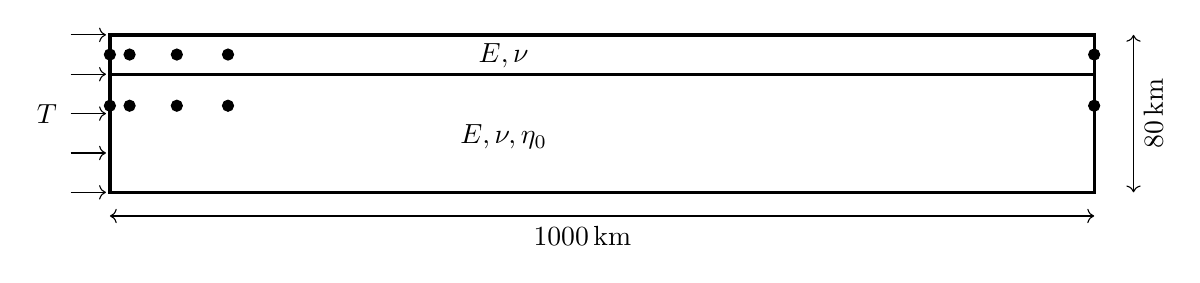
\begin{tikzpicture}
%\draw[step=0.5cm,gray,very thin] (0,0) grid (15,4); %background grid
\draw[very thick] (1,1)--(13.5,1)--(13.5,3)--(1,3)--cycle;  
\draw[very thick] (1,2.5)--(13.5,2.5);  
\draw[<->] (1,0.7)--(13.5,0.7);
\draw[<->] (14,1)--(14,3);
\node[] at (7,0.45) {$\SI{1000}{\km}$};
\node[rotate=90] at (14.25,2) {$\SI{80}{\km}$};
\node[] at (6,2.73) {$E,\nu$};
\node[] at (6,1.7) {$E,\nu,\eta_0$};
\draw[->] (0.5,3)--(0.95,3);
\draw[->] (0.5,2.5)--(0.95,2.5);
\draw[->] (0.5,2)--(0.95,2);
\draw[->] (0.5,1.5)--(0.95,1.5);
\draw[->] (0.5,1)--(0.95,1);
\node[] at (0.2,2) {$T$};

\filldraw[black] (1,2.75) circle (2pt);
\filldraw[black] (1,2.1) circle (2pt);

\filldraw[black] (1.25,2.75) circle (2pt);
\filldraw[black] (1.25,2.1) circle (2pt);

\filldraw[black] (1.85,2.75) circle (2pt);
\filldraw[black] (1.85,2.1) circle (2pt);

\filldraw[black] (2.5,2.75) circle (2pt);
\filldraw[black] (2.5,2.1) circle (2pt);

\filldraw[black] (13.5,2.75) circle (2pt);
\filldraw[black] (13.5,2.1) circle (2pt);
\end{tikzpicture}
\end{center}


After a thorough read of the paper, I have noticed quite a few problems:
\begin{itemize}
\item the paper is old and has been digitized but the figures are missing a lot of lines/shades/points ... this could be remedied by finding the article in a library.
\item in the intro it is stated: "Here we investigate the response of a lithosphere divided into upper elastic and lower uniform visco-elastic layers to simple boundary force and body force systems." The authors later talk about 'isostatic forces' opposing flexure. This means that buoyancy forces should be taken into account but there is no information about densities or gravity values!
\item little uncertainty about boundary conditions. is it free slip or no-slip on the right side ? Looking at fig 4, it looks like the vertical displacement is zero at x=1000km?
\item a Maxwell elasto-viscous rheology is used but this is only mentioned in the Appendix
\item the dimensions of the thinned or thickened areas is simply not mentioned. 
\item Fig~1 shows triangular elements. No mention is made of resolution, type of element, ndofs, resolution tests, any numerical detail whatsoever. Given the age of the paper, I would guess $P_1$
elements.
\item In the appendix they equate the viscous strain rate to $\sigma/4\eta$. Why 4 ?
\item it is also not clear whether the domain is ALE or fully Lagrangian: does it shorten?
\item the value of $T$ is never specified!
\item the paper was published 45 years ago, it is extremely unlikely any of the two authors is still available 
\end{itemize}

\begin{center}
\fbox{\includegraphics[width=16cm]{images/viscoelasticity/kubo77}}\\
{\captionfont Taken from \textcite{kubo77}. Measurement locations are indicated on 
the setup figure above. probably should be reversed}
\end{center}






%..........................................................
\subsection{Parallel-Plate Viscometer Problem - SNAC manual \label{v-e-snac}}

A parallel-plate viscometer problem is simulated, in which viscoelastic material is squeezed between two
parallel plates. The plates are moving at a constant velocity, $v_0$. Each plate has the length of $2L$ and 
is at a distance $2h$ from the other. No slip is assumed between the material and the plates. The approximate
analytical solution is given in the book by \textcite{jaeg69} (1969).

Model Setup: $L = 10~\si{\meter}$, $h=5~\si{\meter}$, viscosity $\eta=10^9~\si{\pascal\second}$, 
bulk modulus $K= 1.5~\si{\giga\pascal}$, shear modulus $\mu = 500~\si{\mega\pascal}$,
$v_0 = 10^{-4}~\si{\meter\per\second}$, $dt = 1~\si{\second}$ (results compared after 500 time steps),
mesh size: $20\times 10~\si{\meter}$, each element is a $1~\si{\meter}$ cube.

Due to the assumption of the original problem setup, artificial forces should be added to left and right
surfaces.

\begin{center}
\includegraphics[width=8cm]{images/viscoelasticity/snac_5}
\includegraphics[width=8cm]{images/viscoelasticity/snac_6}\\
{\captionfont 
Left: The initial mesh (blue) with the velocity boundary condition (red arrows);
Right: The second invariant of stress and velocities plotted on the deformed mesh. Colored arrows are
for SNAC’s solution, black ones for the analytic solution.}
\end{center}

$K=\lambda + \frac23 \mu$ so $\lambda=\frac{3500}{3}MPa$ ?

From wikipedia\footnote{\url{https://en.wikipedia.org/wiki/Lame_parameters}}
\[
\nu = \frac{3K-2\mu}{2(3K+\mu)} 
= \frac{4500-2*500}{2(4500+500)}
= \frac{3500}{10000}
= 0.35
\]
so we find that the material is {\color{orange} compressible $\nu=0.35$}

\[
E=\frac{9K\mu}{3K+\mu} 
=\frac{9*1500*500 MPa^2}{4500+500 MPa}
=\frac{9*1500*500}{5000} MPa
= 1350Mpa
\]


%..........................................................
\subsection{Relaxation after extention - Hassani syllabus}


{\color{orange} compressible $\nu=0.25$}

Un essai de relaxation consiste à imposer à un instant donné une déformation que 
l’on maintient constante par la suite. On observe alors comment évolue la contrainte au cours du temps.

The setup of the experiment is shown in the following figure:

\begin{center}
\includegraphics[width=9cm]{images/viscoelasticity/hassani_1}
\end{center}

The total duration of the experiment is $T=\SI{5}{\year}\simeq \SI{15.75e7}{\second}$.
The duration of the loading is $T/10=\SI{6}{months}$ while the duration 
of the subsequent relaxation is then $9T/10\simeq 4.5~\si{\year}$.

The loading velocity is $v=\SI{1}{\mm\per\year}\simeq \SI{3.17e-11}{\meter\per\second}$.
The sample has size $L\times L/2 = 20\times10\si{cm}$ and 
the strain rate is then $v/L \simeq \SI{1.5e-10}{\per\second}$.
Young's modulus is set to \SI{1e11}{\pascal} and the Poisson ratio is 0.25, i.e.
$\mu=40~\si{GPa}$. The viscosity is set to $\eta_0=\SI{1e18}{\pascal\second}$.
The Maxwell time is then $t_M=\eta/\mu=0.8~\si{\year}$, which is also the time it takes 
to reduce the maximum stress by a factor $e$.

\begin{center}
\includegraphics[width=6cm]{images/viscoelasticity/hassani_2}
\end{center}







%-------------------------------------------------------------------------
\subsection{Role of elasticity in slab bending - \textcite{fogm14} (2014)}

\begin{center}
\includegraphics[width=8cm]{images/viscoelasticity/fogm14b}
\includegraphics[width=8.5cm]{images/viscoelasticity/fogm14c}\\
\end{center}












%-------------------------------------------------------------------------
\subsection{Shear test in 2D - \textcite{famc14} (2014)}

This experiment consists of a viscoelastic material undergoing simple shear at a constant 
rate from a time $t_0$ though to $t_{max}$. At $t_{max}$, the shearing velocity is taken 
to zero using a no-slip velocity boundary condition. The viscoelastic stresses then decay
with time while the material deformation rate remains zero. The $xy$ component of stored 
stress, i.e. the nonviscous portion of the total stress, is given by
\begin{align}
\tau_{xy}^{stor} 
&= 
\exp -\frac{\mu}{\eta}t 
\left(
C_2 \cos\left( \frac{Vt}{h}\right)
-C_1 \sin\left( \frac{Vt}{h}\right)
\right)
-C_2 & \textrm{if} \; t<t_{max} \nn\\
&= \left[\exp -\frac{\mu}{\eta}t_{max} 
\left(
C_2 \cos\left( \frac{Vt}{h}\right)
-C_1 \sin\left( \frac{Vt}{h}\right)
\right)
-C_2 \right] \exp -\frac{\mu}{\eta}(t-t_{max})
& \textrm{if} \; t>t_{max} 
\end{align}
where $V$ is the shear velocity along the top wall boundary, 
$h$ is the height of the box,
\[
C_1=-\frac{V^2 \eta^2 \mu}{\mu^2 h^2 + V^2 \eta^2}
\]
\[
C_2=-\frac{Vh\eta \mu^2}{\mu^2 h^2 + V^2 \eta^2}
\]



\begin{center}
\includegraphics[width=8cm]{images/viscoelasticity/famc14a}\\
\captionfont{The xy component of dimensionless stored stress with dimensionless time 
for the 2-D viscoelastic material undergoing simple shear and relaxation. Nondimensional 
material parameters of $\eta=10^2$, $\mu=10^2$, $t_M=1$, $V=0.05$, $h=1$ 
with $\Delta t_e\in[0.01,1]$ and $\Delta t_c=\frac13 \Delta t_e$.
}
\end{center}

Figure above shows the resulting xy component of the deviatoric stored stress term for a 2-D viscoelastic material across a range of $\Delta t_e$. 
At longer $\Delta t_e$, the stored stress appears under resolved, indicating these larger elastic time step values capture dynamics that occur on time scales approximately equal to or greater than the Maxwell relaxation time, that is with a portion of viscous deformation. For shorter $\Delta t_e$,
the numerically calculated stress approaches the analytic solution, indicating that the elastic time step is
sufficiently small to fully capture the elastic stored stresses produced within the material under the
applied strain rate.







%-------------------------------------------------------------------------
\subsection{Tortion test in 3D - \textcite{famc14} (2014)}

insert here eq 9 of paper

The analytic solution outlined by equation (9) can be extended from this 
essentially 1-D test into 3-D by applying the shear velocity in the x-z plane. 
Testing of the full viscoelastic implementation including the
rotation terms is possible by placing this 3-D shear test in a 
coordinate system under going solid body rotation. 

\begin{center}
\includegraphics[width=8cm]{images/viscoelasticity/famc14b}\\
\captionfont{
The $xy$ and $yz$ stress components of a material undergoing simple shear within 
a 3D rotating reference frame. Nondimensional material parameters of 
$\eta=100$, $\mu=100$, $\alpha=1$, $V=0.3$, $h=1$, $t_{max}=0.5$
and $\omega=42$. Note the coordinate system for this test has the $y$ axis in the vertical 
with the $z$ axis in plane. Results for a first (crosses) and 
fourth- (lines) order accurate Jaumann stress rate integration scheme are shown 
in comparison to the analytical solution (black) given by equation (9) within the rotating frame.
}
\end{center}

Figure above shows the evolution of the stress in comparison to the analytical solution of equation (9)
placed within the rotating frame. The rotating frame is achieved by imposing a velocity boundary condition
of a constant solid body rotation about the y axis in addition to the shearing rate. The stress within this
rotating frame is given by equation (9), with the stress in the nonrotating frame found by 
applying a rotation matrix, $R$, to the nonrotating stress solution. 
That is, $\tau=R^{-1}\tau'R$, where $'$ denotes the rotated frame, $R$ is
the rotation matrix about the y axis given by 
\[
R= \left(
\begin{array}{ccc}
\cos\theta &0 & \sin\theta \\
0 & 1 & 0 \\
-\sin\theta & 0 & \cos\theta
\end{array}
\right)
\]
with $\theta=\omega t$, $\omega$ being the dimensionless rotation rate. 
The stress components shown in Figure 1b from within the 
nonrotating frame can then be given by $\tau^{stor}_{xy}=\tau^{stor'}_{xy} \cos\theta$
and $\tau^{stor}_{yz}=\tau^{stor'}_{yz} \sin\theta$.
It can be seen that, using a higher-order Jaumann stress rate advection scheme 
results in accurate stress advection and rotation within the full
3-D space plus time domain. It should be noted here that the velocity field used in 
this test was chosen to rigorously test the rotational terms in equation (6). 
Whether these rotational terms are required for individual models is dependent upon 
the model setup. For subducting slabs at a constant curvature, the individual 
parcels of material experience purely rotational effects, accounting for this within the stress history term
would then be required for consistency.

{\color{red} finish!}










%-------------------------------------------------------------------------
\subsection{Cylindrical tunnel - Segall book (?)}

{\color{orange} compressible $\nu=0.25$}

communicated to me by L .van de Wiel.

This is a cylindrical tunnel (2D magma chamber) in an infinite space, with certain radius.
The material close around the hole is warm, and and such viscous. The material further from the hole is cold, and purely elastic. (accomplished by setting and absurdly high viscosity) 
There is a clear transition radius between the two properties
The hole contains a pressure, causing the space to expand.

After the initial elastic deformation, viscous deformation continues in the viscous region of the domain.
I have the implementation of the analytical solution attached to save you time.

See plot with radial deformation for t=0 (green), t=300s (red), t=600s (blue), and t=3000s (black).
thin line is analytic, points are numeric.
(with parameters and size parameters as in analytic.f)


\begin{center}
\includegraphics[width=8cm]{images/viscoelasticity/radialDisp}
\end{center}










%..........................................................
\subsection{Relevant literature \& various notes}



\begin{itemize}
\item convection of viscoelastic fluids: 
\textcite{hard91}, \textcite{momy93}, 
\textcite{zhgm96}, \textcite{modm02}, 
\textcite{mure05}, \textcite{likh05a},  
\textcite{likh05b}, \textcite{fukk08}


\item stress buildup associated with viscoelastic rheology 
\textcite{kubo77}, \textcite{kupa84}, \textcite{pocp93}, \textcite{mapo09}

\item viscoelastic effects on geodynamical pbs involving gravitational instability 
\textcite{pocp93,kabe07,bumo08,scbe08}, 
\textcite{hamy95} 

\item large strain  eulerian viscoelasticity 
\textcite{scps01,vapy01,coll06,moql07,fukk08,poso08}

\end{itemize}

\textcite{famc14} states 
``Funiciello et al. [2003] implemented a viscoelastic rheology in numerical models of subduction, performing a
range of numerical simulations to investigate its effect on subducting slab dynamics. Similar methodologies have addressed the details of viscoelastic stress within the bending zone during subduction, although a comparison between viscous and viscoelastic rheology was lacking [Capitanio et al., 2009; Capitanio and Morra, 2012].
Muhlhaus and Regenauer-Lieb [2005] and Moresi et al. [2002] have studied the role of elasticity in mantle convection, comparing the viscous case to that of viscoelastic, and Kaus and Becker [2007] discussed the effect of elasticity on layered Rayleigh-Taylor instabilities. However, a systematic study into the effects of elastic stresses on models of free subduction has yet to be completed. Morra and Regenauer-Lieb [2006], Funiciello et al. [2003], Capitanio et al. [2007], Yamato et al. [2007], and Royden and Husson [2006] have included a viscoelastic slab in subduction models, without explicitly studying the effects of the elastic component across a range of parameters.''


Check early paper by Braun \& Beaumont (1987) \cite{brbe87}

\textcite{asmo12} (2012)
\textcite{hepk14} (2014)
\textcite{daws16} (2016)
\textcite{thkp15} (2015)
\textcite{beps10} (2010)
\textcite{samb20} (2020)
\textcite{vosc15} (2015)
\textcite{nalr12} (2012)
\textcite{pelt74} (1974)
 \label{chapt:viscoelasticity} %%%%%%%%%%%%%%%%%%%%%%%%%%%%%%%%%%%

%%%%%%%%%%%%%%%%%%%%%%%%%%%%%%%%%%%%%%%%%%%%%%%%%%%%%%%%%%%%%%%%%%%%%%%%%%%%%%%%%%%%%%%%%%%%%%%%%%%
%\chapter{Geophysical data} %%%%%%%%%%%%%%%%%%%%%%%%%%%%%%%%%%%%%%%%%%%%%%%%%%%%%%%%%%%%%%%%%%%%%%%
\chapter{Geophysical data} 

\newpage %-----------------------------------------------------------------------------------------
\section{The PREM model} \label{ss:prem} \input{prem} %--------------------------------------------
\newpage %-----------------------------------------------------------------------------------------
\section{From 1D tomography to density/temperature} \begin{flushright} {\tiny {\color{gray} \tt dlvsdlnro.tex}} \end{flushright}
%~~~~~~~~~~~~~~~~~~~~~~~~~~~~~~~~~~~~~~~~~~~~~~~~~~~~~~~~~~~~~~~~~~~~~~~~~~~

The mantle is heterogeneous but it is also inaccessible. This means that 
one must rely on indirect methods 
to probe its structure. Seismic tomography is a technique for imaging 
the subsurface of the Earth with seismic waves produced by earthquakes or explosions. 
P-, S-, and surface waves can be used for tomographic models of different resolutions.

Seismic velocity is a meaningful parameter for the interior dynamics of the
Earth because there exists a direct relation between seismic velocity and density. 
Such a relation was analysed experimentally by (for instance) Barton (1986) who 
used laboratory measurements of P-wave seismic velocity and density of rocks \cite{bart86}. 

Fourty years later or so, a crucial question remains: what is the exact form of the 
relation between density and seismic velocity for the entire Earth's mantle?

I will here not go into the details of the underlying theories and 
their approximations but will show a few useful results. 

From tomography to density, the workflow is usually as follows:
\[
d \ln V_p \rightarrow d \ln V_s \rightarrow d \ln \rho \rightarrow d\rho
\]
Note that if the method is based on shear wave tomography the conversion $d \ln V_p \rightarrow d \ln V_s$
is not necessary. 
Also the last step $d \ln \rho \rightarrow d\rho$ requires a background density field, 
often taken to be either the PREM model or AK135 (see Section~\ref{ss:prem}). 

On the following plots are shown radial averages of the 
ratio $d \ln V_s/d\ln V_p$ and/or $d\ln \rho/d \ln V_s$:

\begin{center}
\includegraphics[width=7cm]{images/thermal_expansion/pape95}\\
{\captionfont Taken from \textcite{pape95} (1995).}
\end{center}

\begin{center}
\includegraphics[height=5cm]{images/dlnvsdlnrho/moek16b}
\includegraphics[height=5cm]{images/dlnvsdlnrho/moek16a}\\
{\captionfont Taken from Moulik \& Ekstrom (2016) \cite{moek16}}
\end{center}

\begin{center}
\includegraphics[height=6cm]{images/dlnvsdlnrho/xi.pdf}\\
{\captionfont Profiles of scaling factor $\xi=d \ln \rho/d\ln V_s$. Data from 
Steinberger \& Calderwood (2006) \cite{stca06} and Moulik \& Ekstrom (2016) \cite{moek16}.
Data available in images/dlnrhodlnvs/} 
\end{center}

Then
\[
\delta \ln(\rho(r,\theta,\phi)) = \xi(r) \cdot \delta \ln (V_s(r,\theta,\phi) )
\]
with  
\[
\delta \ln (\rho(r,\theta,\phi)) = \frac{ \delta \rho(r,\theta,\phi)}{\rho_{ref}(r)}
\]
where $\rho_{ref}$ is a radial profile, PREM for instance in the case of S40RTS 
so finally 
\[
\delta \rho(r,\theta,\phi) 
= \rho_{ref}(r) \cdot  \delta \ln(\rho(r,\theta,\phi)) 
= \rho_{ref}(r)\cdot \xi(r) \cdot \delta \ln(V_s(r,\theta,\phi)) 
\]






\Literature: \cite{roma01}
 %----------------------------
\newpage %-----------------------------------------------------------------------------------------
\section{Earth radial viscosity profile \label{ss:viscprof}} \begin{flushright} {\tiny {\color{gray} \tt viscosity\_profile.tex}} \end{flushright}
%~~~~~~~~~~~~~~~~~~~~~~~~~~~~~~~~~~~~~~~~~~~~~~~~~~~~~~~~~~~~~~~~~~~~~~~~~~~~~~~~~~~~~~~~~~~~~~~~~~


\begin{center}
\includegraphics[width=6cm]{images/viscosity_profile/hamy95}\\
{\captionfont \nineteenninetyfive: Taken from Hanyk \etal (1995) \cite{hamy95}. 
$\eta(z)=(1+214.3z\exp-16.7(0.7-z)^2)\times 10^{21}\si{pascal\second}$ }
\end{center}

\begin{center}
\includegraphics[width=6cm]{images/viscosity_profile/csyu97}\\
{\captionfont \nineteenninetyseven: Taken from Cserepes \& Yuen (1997) \cite{csyu97}} 
\end{center}

\begin{center}
\includegraphics[width=8cm]{images/viscosity_profile/pape98}\\
{\captionfont \nineteenninetyeight: Taken from \textcite{pape98} (1998).} 
\end{center}

\begin{center}
\includegraphics[width=5cm]{images/viscosity_profile/yohk01}\\
{\captionfont \twothousandone:Radial viscosity profile of the reference model. 3-layered model is adopted: 
the lithosphere (0 km to 150 km), the upper mantle (150 km to 670km) 
and the lower mantle (670 km to 2900 km). Taken from \cite{yohk01}}
\end{center}


\begin{center}
\includegraphics[height=6cm]{images/viscosity_profile/profiles_steinberger}
\includegraphics[height=6cm]{images/viscosity_profile/stca06-fig4}\\
{\captionfont \twothousandsix:
Non-optimized, normalized viscosity profiles, as sent by B. Steinberger,
corresponding to fig.~4 in Steinberger \& Calderwood (2006) \cite{stca06}.}
\end{center}

\begin{center}
\includegraphics[height=6cm]{images/viscosity_profile/mofm08}\\
{\captionfont Taken from \textcite{mofm08} (2008).}
\end{center}


\begin{center}
\includegraphics[width=11cm]{images/viscosity_profile/capd11}\\
{\captionfont \twothousandeleven: Taken from Cadio \etal \cite{capd11}.
Mantle viscosity structure employed in calculating synthetic geoid anomalies. 
Red: VR (Ricard \etal, 1993); Blue: VMF (Mitrovica and Forte, 2004); Cyan: VMF-LVZ (Mitrovica
and Forte, 2004); Green: VSC (Steinberger and Calderwood, 2006); Orange: VYN (Yoshida and Nakakuki, 2009).}
\end{center}

\begin{center}
\includegraphics[width=11cm]{images/viscosity_profile/civs12-fig1}\\
{\captionfont \twothousandtwelve: Taken from Ciskova \etal \cite{civs12}.}
\end{center}

\begin{center}
\includegraphics[width=6cm]{images/viscosity_profile/kaps14}\\
{\captionfont \twothousandfourteen Taken from Kaban \etal  \cite{kaps14}.
(Black) reference radial viscosity from (Steinberger and Calderwood 2006); 
(Blue) alternative viscosity model of Kaban and Trubitsyn (2012); 
(Light Grey) limits of viscosity variations in the model with LVV (Petrunin \etal 2013).
}
\end{center}

\begin{center}
\includegraphics[width=14cm]{images/viscosity_profile/profiles}\\
{\captionfont Steinberger (2016) \cite{stei16}; 
Ciskova \etal (2012) \cite{civs12}.}
\end{center}

\begin{center}
\includegraphics[width=5cm]{images/viscosity_profile/kani19}\\
{\captionfont \twothousandnineteen: Taken from Kaneko \etal \cite{kani19} (2019).}
\end{center}

\begin{center}
\includegraphics[width=6cm]{images/viscosity_profile/nemi23}\\
{\captionfont \twothousandtwentythree: Taken from \textcite{nemi23} (2023).}
\end{center}

\begin{center}
\includegraphics[width=10cm]{images/viscosity_profile/pldp24}\\
{\captionfont \twothousandtwentyfour: Taken from \textcite{pldp24} (2024).}
\end{center}



\Literature:
\begin{itemize} 
\item Viscosity profile of the lower mantle \cite{elss85}
\item Matyska \etal (2011) \cite{mayw11}
\item Flament (2019) \cite{flam19}
\item Mitrovica \& Forte \cite{mifo04}
\item King \& Masters \cite{kima92}
\item Rudolph \etal \cite{rull15}
\item steinberger \& holme \cite{stho08}
\item steinberger \cite{stei16}
\item Cadek \& Yuen \cite{cayu93}
\item supp of \cite{badw17}
\end{itemize} 
 %-----------
\newpage %-----------------------------------------------------------------------------------------
\section{Earth radial temperature profile \label{ss:adiab}} \begin{flushright} {\tiny {\color{gray} adiabatic.tex}} \end{flushright}
%~~~~~~~~~~~~~~~~~~~~~~~~~~~~~~~~~~~~~~~~~~~~~~~~~~~~~~~~~~~~~~~~~~~~~~~~~~~~~~~~~~~~~~~~~~~~~~~~~~

The method of manufactured solutions is a relatively simple way of carrying out

We start by the first sentence of Bunge (2005) \cite{bung05}:
"The average temperature increase through Earth's
crust and mantle is called the geotherm. Its basic form is
assumed to consist of adiabatic regions where temperatures 
rise only slightly with depth, and of narrow thermal
boundary layers where temperatures increase rapidly
over a depth of a few hundred kilometers (Jeanloz and
Morris, 1986) \cite{jemo86}."

Before we look further at the equations behind this temperature profile, 
we must look at the basic assumption we make about
the type of convection taking place in the mantle:
layered convection vs. whole mantle convection, as
depicted here: 

\begin{center}
\includegraphics[width=12cm]{images/adiabatic/modes}\\
{\captionfont Taken from \url{https://geologyengineering.com/2020/05/mantle-convection/}}
\end{center}

\noindent Indeed, the type of convection is then expected to have an strong influence 
on the radial temperature profile: 

\begin{center}
\includegraphics[width=10cm]{images/adiabatic/drawing.png}
\end{center}

This is also to be found in Poirier's book \cite{poirier}:
\begin{center}
\includegraphics[width=11cm]{images/adiabatic/poirier}\\
{\captionfont Schematic diagrams of (a) whole-mantle and (b) layered convection
models, with corresponding temperature and viscosity profiles (after 
Peltier \& Jarvis (1982) \cite{peja82}.)}
\end{center}


The two-layered convection hypothesis relies essentially 
on the viscosity jump at the 660 discontinuity and seems 
to be generally accepted.
It also forms the basis of {\v{C}}adek \& van den Berg (1998) \cite{cava98}
in which the authors carry out an inversion to obtain 
radial profiles of temperature and viscosity in the Earth's mantle
inferred from the geoid and lateral seismic structure:
\begin{center}
\includegraphics[width=6cm]{images/adiabatic/cava98a.png}
\includegraphics[width=5.5cm]{images/adiabatic/cava98b.png}\\
{\captionfont Taken from \cite{cava98}. 
Left: Parameterization of the geotherm used in the paper;
Right: Four model geotherms reducing the misfit by 70\%. The
differences between the models illustrate uncertainties of the
solution.}
\end{center}

More recently, Katsura \etal (2010) \cite{kayy10} have constructed the following mantle temperature 
and temperature gradient profiles:

\begin{center}
\includegraphics[width=6cm]{images/adiabatic/kayy10a}
\includegraphics[width=6cm]{images/adiabatic/kayy10b}\\
{\captionfont Taken from Katsura \etal (2010) \cite{kayy10}.
Left: The adiabatic temperature distributions in the mantle. The three solid lines
denote the temperature distributions proposed in this study using three different
pressure scales. Those proposed by the previous studies are shown for comparison
(BS81: Brown and Shankland, 1981; IK89: Ito and Katsura, 1989; dS00: da Silva \etal,
2000; SD08: Stacey and Davis, 2008). The mantle solidus proposed by Hirschmann
(2000) is also shown.
Right:
Adiabatic temperature gradient in the mantle. The adiabatic temperature gradient 
abruptly increases in association with the olivine-wadsleyite,
wadsleyite-ringwoodite, ringwoodite-perovskite + periclase transitions, as is the
case for the thermal expansion. The adiabatic temperature gradients given in the
previous studies are also shown for comparison (BS81: Brown and Shankland, 1981;
SD08: Stacey and Davis, 2008 \cite{stacey_davis}).
}
\end{center}


\begin{center}
\includegraphics[width=10cm]{images/adiabatic/nemi23}\\
{\captionfont Taken from \textcite{nemi23}.}
\end{center}


Prof. Steinberger was gracious to communicate to me the data of Steinberger \& Calderwood (2006) \cite{stca06}:
\begin{center}
\includegraphics[width=8.5cm]{images/adiabatic/steinberger/Tprofile.pdf}
\includegraphics[width=8.5cm]{images/adiabatic/steinberger/Tprofile_upper.pdf}\\
{\captionfont Temperature profiles from Steinberger \& Calderwood \cite{stca06}.}
\end{center}

One can gather data from various papers and books and this yields the following 
figure\footnote{It must be said that finding actual data -not figures- is remarkably difficult.}:

\begin{center}
\includegraphics[width=8.5cm]{images/adiabatic/Tprofile.pdf}
\includegraphics[width=8.5cm]{images/adiabatic/Tprofile_upper.pdf}\\
{\captionfont 
Note that the T values of Stacey (1977) \cite{stac77} inexplicably go to 540-550K at the surface. 
The value 545 has therefore been subtracted from the values in the paper. These then 
align remarquably well with those of Katsura \etal
}
\end{center}




We see that there is a remarkable agreement between many studies for the temperature down to 400km 
depth. Most show a step in the profile between 400 and 670km depth but the temperature at 670km
depth seems to be between 1650$\si{\celsius}$ and 1750$\si{\celsius}$.
Further down, the discrepancy between studies increases (effectively boiling down to 
the value of the adiabatic gradient). 100km above the CMB all studies seem to indicate a 
temperature of 2300-2400$\si{\celsius}$. Temperature values at the CMB differ a lot and 
as noted in Bull \etal (2009) \cite{bumr09}: 
"Estimates of CMB temperature vary greatly. [...] 
We impose a surface temperature of 273 K and
investigate three CMB temperatures: 3000 K (consistent with
previous studies of this nature, e.g., Kellogg \etal., 1999 \cite{kehv99}), 3950 K
(consistent with recent results on the double-crossing of Post-
Perovskite, e.g., Hernlund \etal., 2005 \cite{hett05}; van der Hilst \etal, 
2007 \cite{vadw07}; Alf\`e \etal., 2002), and 4800 K (Knittle and Jeanloz, 1991). The 3950 K
temperature is the 'reference' temperature which we use for the
majority of cases."
The CMB temperature is set to $2900-3200\si{\celsius}$ in Fowler \cite{fowler}.


Also, oceanic plates being thinner than continental plates (alongside with different 
radiogenic decay and thermal properties) one can draw two representative mantle 
geotherms \cite{tusc}:

\begin{center}
\includegraphics[width=4cm]{images/adiabatic/tusc.png}\\
{\captionfont Taken from Turcotte \& Schubert \cite{tusc}}
\end{center}




\newpage



[from ASPECT manual]



---------------------------------------------
\paragraph{Isentropic gradient}

The material properties also define the slope of the adiabat (the change in temperature with
pressure at constant entropy) at all pressures and temperatures. Using the cyclic relation,
we can define this slope in terms of partial differentials of the entropy with respect to pressure
and temperature:
\begin{eqnarray}
\left( \frac{\partial T}{\partial p} \right)_{S} 
&=& - \left( \frac{\partial T}{\partial S} \right)_{p} \left( \frac{\partial S}{\partial p} \right)_{T} \\
&=& - \left( \frac{T}{C_p} \right) \left( - \frac{\alpha}{\rho} \right) \\
&=& \frac{\alpha T}{\rho C_p} \label{eq:mm_isentropic_gradient}
\end{eqnarray}
This expression does not pose a constraint on the material properties, but in order to be 
self-consistent, the adiabat must be computed following this relation.

For complex material models, obtaining analytical functions which obey all these relations
may be a non-trivial exercise. Furthermore, it is often not immediately clear when a
given formulation is thermodynamically inconsistent. Indeed, both the
thermodynamic and the geodynamic literature contain many equations of
state and material parameterizations which do not obey these 
relations! This may not invalidate the results obtained with these 
models, but it is a point worth keeping in mind as the geodynamics
community moves to more complicated and more realistic parameterizations.

\emph{A final note of warning: Some compressible formulations in \aspect{}
  (Section~\ref{sec:mass-conservation-approximation}) use the isothermal compressibility,
  while others use the isentropic compressibility. Fully self-consistent material models must
  either specify what approximation of the compressible equations they are consistent with
  (see Section~\ref{sec:approximate-equations}), or have a switch so that they use the correct
  compressibility for each of the different approximations. The conversion between isothermal
  and isentropic compressibilities is given in~\eqref{eq:mm_isentropic_compressibility}.}

--------------------------------------------------

\paragraph{Initial conditions and the adiabatic pressure/temperature}

The thermo-mechanically coupled (Navier-)Stokes 
equations require us to
pose initial conditions for the temperature
Note that the equations
themselves do not require that initial conditions are specified for
the velocity and pressure variables (since there are no time
derivatives on these variables in the model).

Nevertheless, a nonlinear solver will have difficulty converging to
the correct solution if we start with a completely unphysical pressure
for models in which coefficients such as density $\rho$ and viscosity
$\eta$ depend on the pressure and temperature. To this end, \aspect{}
uses pressure and temperature fields $p_{\textrm{ad}}(z),
T_{\textrm{ad}}(z)$ computed in the adiabatic conditions model
(see Section~\ref{parameters:Adiabatic_20conditions_20model}).
By default, these fields satisfy adiabatic conditions:
\begin{align}
\rho C_p \frac{\textrm{d}}{\textrm{d}z} T_{\textrm{ad}}(z)
&=
\frac{\partial\rho}{\partial T} T_{\textrm{ad}}(z) g_z,
\\
\frac{\textrm{d}}{\textrm{d}z} p_{\textrm{ad}}(z)
&=
\rho g_z,
\end{align}
where strictly speaking $g_z$ is the magnitude of the vertical
component of the gravity vector field, but in practice we take the
magnitude of the entire gravity vector.

These equations can be integrated numerically starting at $z=0$, using
the depth dependent gravity field and values of the coefficients
$\rho=\rho(p,T,z), C_p=C_p(p,T,z)$. As starting conditions at $z=0$ we
choose a pressure $p_{\textrm{ad}}(0)$ equal to the average surface
pressure (often chosen to be zero, see Section~\ref{sec:pressure}),
and an adiabatic surface temperature $T_{\textrm{ad}}(0)$ that is
also selected in the input parameter file.
%\index[prmindex]{Adiabatic surface temperature}
%\index[prmindexfull]{Adiabatic surface temperature}

\note{The adiabatic surface temperature is often chosen significantly
  higher than the actual surface temperature. For example, on earth,
  the actual surface temperature is on the order of 290 K, whereas a
  reasonable adiabatic surface temperature is maybe 1600 K. The reason
  is that the bulk of the mantle is more or less in thermal equilibrium
  with a thermal profile that corresponds to the latter temperature,
  whereas the very low actual surface temperature and the very high
  bottom temperature at the core-mantle boundary simply induce a
  thermal boundary layer. Since the temperature and pressure profile
  we compute using the equations above are simply meant to be good
  starting points for nonlinear solvers, it is important to choose
  this profile in such a way that it covers most of the mantle well;
  choosing an adiabatic surface temperature of 290 K would yield a
  temperature and pressure profile that is wrong almost throughout the
  entire mantle.}

For instance, let us consider $\alpha=3\cdot 10^{-5}$, 
$g_z=10$, $C_p=1250$, $\rho=\rho_0(1-\alpha (T-T_0)$ so that 
$\frac{\partial\rho}{\partial T} = -\alpha \rho_0$ 
with $\rho_0=3300$.

Then we must solve the following equation
\[
\rho_0(1-\alpha(T-T_0)) C_p \frac{\textrm{d}T}{\textrm{d}z} 
=
- \alpha T^2  g_z
\]

----------------------------------

In Verhoogen (1951) \cite{verh51}:
As is well known, the adiabatic gradient may be written as
\[
\frac{dT}{dP} = \alpha T /\rho C_p
\]
If hydrostatic equilibrium is assumed, the pressure varies with depth $h$ as 
$dP = \rho g dh$, so that
\[
\frac{d \ln T}{dh} = \frac{\alpha g}{C_p}
\]
from which the temperature $T$ at any depth $h$ may be computed as a function of the temperature
at any assigned depth if the ratio $\alpha/C_p$ 
is known at all depths ($g$, the acceleration of gravity, will
be taken as constant in the mantle).

----------------------------------


----------------------------------

From DyMaLi: In the interior of a convecting medium temperatures follow an adiabatic profile. 
At the top and bottom of a convecting layer thermal boundary layers with large thermal gradients form. 
The interior is thermally well mixed and therefore essentially isothermal, with a slight increase 
of temperatures with depth due to the effect of pressure.
For example in the Earth's mantle the geothermal gradient $\partial T /\partial z$ 
is about 20C/km near the 
surface and about 0.3C/km in the interior of the mantle. This small gradient in the 
interior is the adiabatic gradient. If a small
volume of material is moved to shallower depth is experiences a slight increase in volume 
due to the decreasing pressure and associated with this a slight decrease in temperature. 
This change in temperature is the adiabatic temperature change.

The adiabatic gradient can be determined from the thermodynamics relation between entropy per unit mass S,
temperature T, and pressure P:
\[
dS = \left( \frac{dS}{dT}\right)_P dT +  \left( \frac{dS}{dP}\right)_T dP
=
\frac{C_p }{T} dT - \frac{\alpha}{\rho} dP
\]
In case of a reversible adiabatic process the entropy change is zero, and so the adiabatic gradient is:
\[
\left( \frac{dT}{dP}\right)_S = \frac{\alpha T}{\rho C_p} 
\]
The gradient can also be expressed in terms of depth, remembering that $d p = \rho gdz$ 
in a hydrostatic fluid:
\[
\left( \frac{dT}{dz}\right)_S = \frac{\alpha g T}{C_p} 
\]
Thus to determine the adiabatic gradient one needs values of $\alpha$ 
and $C_p$ with depth. These are obtained from laboratory experiments.

One also needs an estimate of density as a function of depth, which is generally determined
from seismology. 
Integration of the adiabatic gradient in terms of pressure then gives
temperature as a function of pressure. 
Temperature as a function of depth is obtained by integrating the density
distribution to obtain g as a function of depth.

not finished
----------------------------------

Vol07\_02

This adiabaticity hypothesis should, however, not
be taken too literally (Jeanloz and Morris, 1987 \cite{jemo87}). In
most numerical simulations, the resulting averaged
geotherm can be far (a few hundred kelvins) from
adiabatic (Bunge \etal, 2001 \cite{burm01}). First, radioactive 
heating, dissipation, and diffusion are never totally
negligible, second, even if each fluid parcel follows
its own adiabatic geotherm, the average geotherm
may not correspond to any particular adiabat.



----------------------------------
From Steinberger oct 26th, 2020:

Yes, I think the temperature below the lithosphere is still fairly well-constrained, based on magmas produced on mid-oceanic ridges (away from plumes) if one takes these as representative. Regarding Dannberg and Sobolev (not Solomatov!) I don't know why it is lower. In their supplementary figures, the extrapolation to the surface is actually $\sim 1250\si{\kelvin}$, not $1250\si{\celsius}$, which is even less. Perhaps best to directly ask Juliane about this.

How the temperature increases with depth is more uncertain; the temperature gradient is often taken as adiabatic; that's what I also assumed in the 2006 paper, then it is defined by a ordinary differential equation (eq. 12 in that paper). I think the main uncertainty is the thermal expansivity. In my model, it strongly decreases with depth, I guess that is why my models have a lower temperature in the lower mantle than other models. I think that strong decrease in expansivity is still the consensus, but I didn't closely follow the literature recently. But the temperature gradient between the thermal boundary layers may actually be subadiabatic, hence even lower, due to cold slabs sinking to and accumulating above the CMB, and hot plume material feeding into the asthenosphere, below the lithosphere. So, yes, I would say the difference in the deep mantle (if not more) reflects the current state in the community.

And I think the uncertainites of CMB temperature are even larger. And I would of course be happy if you host my data on a public github repo. Just for the viscosity profile, there should be some explanation given that it shouldn't necessarily be taken "at face value" but that (like in the 2006 paper) it is possible to multiply different parts of the profile with different "scaling viscosities".

----------------------------------

\Literature: 
{\it On the thermal gradient in the Earth's deep interior}, Tirone (2016) \cite{tiro16} \\
{\it Is the mantle geotherm subadiabatic}, Jeanloz \& Morris (1987) \cite{jemo87} \\
{\it Mantle convection, the asthenosphere, and Earth's thermal history} King (2015) \cite{king15}\\

check section 7.7 in Fowler !

boundary layer jape82

evolution shpe79
 %--------------------
\newpage %-----------------------------------------------------------------------------------------
\section{Earth radial thermal expansion profile} \begin{flushright} {\tiny {\color{gray} thermal\_expansion\_profile.tex}} \end{flushright}


\begin{center}
\includegraphics[width=7cm]{images/thermal_expansion/pape95}\\
{\captionfont 
Taken from \textcite{pape95} (1995).}
\end{center}

\begin{center}
\includegraphics[width=10cm]{images/thermal_expansion/buja04}\\
{\captionfont 
Taken from \textcite{buja04} (2004). To dimensionalize, multiply 
the thermal expansivity (thick solid line) 
by $\alpha_0=2\cdot 10^{-5}~\si{\per\kelvin}$.
}
\end{center}


\begin{center}
\includegraphics[width=10cm]{images/thermal_expansion/stca06.jpg}\\
{\captionfont Taken from \textcite{stca06}.}
\end{center}

see Matyska \etal (2011) \cite{mayw11}

Mantle convection with internal heating and pressure-dependent thermal expansivity, Leitch \etal (1991) \cite{leys91}

Eq(8) of Hassan \etal \cite{hafg15}

\begin{center}
\includegraphics[width=10cm]{images/thermal_expansion/nemi23}\\
{\captionfont Taken from \textcite{nemi23}.}
\end{center}
 %---------------
\newpage %-----------------------------------------------------------------------------------------
\section{Earth radial density profile} \begin{flushright} {\tiny {\color{gray} density\_profile.tex}} \end{flushright}
%~~~~~~~~~~~~~~~~~~~~~~~~~~~~~~~~~~~~~~~~~~~~~~~~~~~~~~~~~~~~~~~~~~~~~~~~~~~~~~~~~~~~~~~~~~~~~~~~~~

\begin{center}
\includegraphics[width=12cm]{images/density_profile/density_profile}
\end{center}

\Literature: Kennett (1998) \cite{kenn98}

\textcolor[RGB]{220,220,220}{\rule{\linewidth}{0.2pt}}

\begin{center}
\includegraphics[width=8cm]{images/density_profile/chmo95}\\
{\captionfont Taken from \textcite{chmo95} (1995).
A model for average crustal petrology versus depth consistent with average velocity depth
profile (solid circles) and velocity depth curves for common rock types (open symbols). 
Variations of density and SiO 2 content with depth are from rock percentages
shown on the left.} 
\end{center}


\textcolor[RGB]{220,220,220}{\rule{\linewidth}{0.2pt}}

Let us look at the density and pressure profiles in a 1D isothermal 'planet'. 
We start from 
\[
-\vec\nabla p + \rho \vec{g} = \vec{0}
\]
In 1D, and assuming $\vec{g}=-g \vec{e}_z$:
\[
-\frac{dp}{dz}-\rho g=0
\]
or
\[
\frac{dp}{dz}= -\rho g
\]
Assuming $\rho$ and $g$ constant in the domain $z\in [0,L]$, we can solve this ODE and we obtain:
\[
p(z) = \rho g (L-z)
\]
Let us now turn to the case of an isothermal but compressible fluid. 
Its density is now given by 
\[
\rho(p) = \rho_0(1-\beta p)
\]
where $\beta$ is the compressibility (assumed to be constant in the domain). We must then solve
\begin{eqnarray}
\frac{dp}{dz}= -\rho_0(1-\beta p) g
&\Rightarrow&
\frac{dp}{1-\beta p} = -\rho_0 g dz \nonumber\\
&\Rightarrow&
\int \frac{dp}{1-\beta p} = -\int \rho_0 g dz \nonumber\\
&\Rightarrow&
-\frac{1}{\beta} \ln (1-\beta p) = -\rho_0 g z + C \nonumber\\
&\Rightarrow&
\ln (1-\beta p) = \beta \rho_0 g z + D \nonumber\\
&\Rightarrow&
1 -\beta p = \exp \left( \beta \rho_0 g z + D  \right) \nonumber\\
&\Rightarrow&
p(z) = \frac{1}{\beta} \left[ 1- \exp \left( \beta \rho_0 g z + D  \right) \right] \nonumber\\
\end{eqnarray}
At $z=L$ we require $p=0$ so we obtain
\[
p(z) = \frac{1}{\beta} \left[ 1- \exp \left( \beta \rho_0 g (z-L)  \right) \right]
\]
Note that when the compressibility tends to zero, by virtue of 
\[
\exp x \sim 1 + x + \frac{x^2}{2} + ...
\]
for $x\rightarrow 0$ we then recover the linear pressure profile above.

Let us now take $\rho_0=\SI{4000}{\kg\per\cubic\meter}$, 
$g=\SI{10}{\meter\per\square\second}$ and $\beta=4\cdot 10^{-12}~\si{\per\pascal}$ \cite{gadb20} 
and $L=3000~\si{\km}$.

\begin{center}
\includegraphics[width=12cm]{images/density_profile/pressure}
\end{center}

TODO: produce same plot with density

\begin{center}
\includegraphics[width=6cm]{images/density_profile/nemi23}\\
{\captionfont Taken from \textcite{nemi23}.}
\end{center}
 %-----------------------------------
\newpage %-----------------------------------------------------------------------------------------
\section{Earth radial thermal conductivity profile} \begin{flushright} {\tiny {\color{gray} thermal\_conductivity\_profile.tex}} \end{flushright}

\begin{center}
\includegraphics[width=10cm]{images/thermal_conductivity/nemi23}\\
{\captionfont Taken from \textcite{nemi23}.}
\end{center}
 %---------
 \label{chapt:geophysical_data} %%%%%%%%%%%%%%%%%%%%%%%%%%%%%%%%%


%%%%%%%%%%%%%%%%%%%%%%%%%%%%%%%%%%%%%%%%%%%%%%%%%%%%%%%%%%%%%%%%%%%%%%%%%%%%%%%%%%%%%%%%%%%%%%%%%%%
%%%%%%%%%%%%%%%%%%%%%%%%%%%%%%%%%%%%%%%%%%%%%%%%%%%%%%%%%%%%%%%%%%%%%%%%%%%%%%%%%%%%%%%%%%%%%%%%%%%
\appendix %%%%%%%%%%%%%%%%%%%%%%%%%%%%%%%%%%%%%%%%%%%%%%%%%%%%%%%%%%%%%%%%%%%%%%%%%%%%%%%%%%%%%%%%%
%%%%%%%%%%%%%%%%%%%%%%%%%%%%%%%%%%%%%%%%%%%%%%%%%%%%%%%%%%%%%%%%%%%%%%%%%%%%%%%%%%%%%%%%%%%%%%%%%%%
%%%%%%%%%%%%%%%%%%%%%%%%%%%%%%%%%%%%%%%%%%%%%%%%%%%%%%%%%%%%%%%%%%%%%%%%%%%%%%%%%%%%%%%%%%%%%%%%%%%

\chapter{Matrix properties} \input{matrices} %%%%%%%%%%%%%%%%%%%%%%%%%%%%%%%%%%%%%%%%%%%%%%%%%%%%%%
\chapter{Don't be a hero - unless you have to} \input{hero} %%%%%%%%%%%%%%%%%%%%%%%%%%%%%%%%%%%%%%%
\chapter{Some useful Python commands} \begin{flushright} {\tiny {\color{gray} app\_useful\_python.tex}} \end{flushright}

%--------------------------
\subsection{Sparse matrices}

So far, the best way I have found to deal with sparse matrices is to 
declare the matrix as a 'lil\_matrix' (linked list).

\begin{lstlisting}
from scipy.sparse import csr_matrix, lil_matrix
A_mat = lil_matrix((Nfem,Nfem),dtype=np.float64)
\end{lstlisting}

One then adds terms to it as if it was a full/dense matrix. 
Once the assembly is done, the conversion to CSR format is trivial:

\begin{lstlisting}
A_mat=A_mat.tocsr()
\end{lstlisting}

Finally the solver can be called:

\begin{lstlisting}
sol=sps.linalg.spsolve(A_mat,rhs)
\end{lstlisting}

%--------------------------
\subsection{condition number}

if the matrix has been declared as lil\_matrix, first convert it to a dense matrix:
\begin{lstlisting}
A_mat=A_mat.dense()
\end{lstlisting}
The condition number of the matrix is simply obtained as follows:
\begin{lstlisting}
from numpy import linalg as LA
print(LA.cond(A_mat))
\end{lstlisting}

%--------------------------
\subsection{Weird stuff}

Python is touted as the one language students should learn 
and master. However it is a language which allows *way* too 
much liberty in its syntax and encourages students to be sloppy. 

For instance the following code runs just fine:

\begin{lstlisting}
for k in range(0,5): 
    for k in range(0,5):
        for k in range(0,5):
            print (k)
\end{lstlisting}

This alone should disqualify this language. It is easy to see the obvious problem with this code, but adding a few lines of code in between each 'for' line hides the problem and the absence of any warning makes this code a nightmare to debug.

Here is another example:

\begin{lstlisting}
import numpy as np

Told=np.full(10,123)

Tnew=np.zeros(10)
for i in range(0,10):
    Tnew[i]=np.sqrt(i**5)

print(Tnew)

Told[:]=Tnew[:]

print(Told)
\end{lstlisting}
If Told is not defined explicitely as a float, then the 
numer 123 will decide of its type (in this case 
integer). If `123' is changed into `123.' then the 
array will be initialised as an array of floats.
In the first case 
\begin{verbatim}
Told is [  0   1   5  15  32  55  88 129 181 243]
\end{verbatim}
while in the second case it is equal to 
\begin{verbatim}
[  0.           1.           5.65685425  15.58845727  32.
  55.90169944  88.18163074 129.64181424 181.01933598 243.        ] 
\end{verbatim}
This is very dangerous since our students are not taught 
number representation.

\begin{verbatim}
https://www.w3schools.com/python/default.asp

https://www.codecademy.com/learn/learn-python

https://learnpythonthehardway.org/book/
\end{verbatim}

%----------------------------------
\subsection{Making simple 2D plots}

\begin{lstlisting}
import matplotlib.pyplot as plt

# number of points
N=100

# a despicable way of filling two arrays
x_data=[]
y_data=[]
for i in range(0,N):
    x=i
    y=i**2+2*i+1.
    x_data.append(x)
    y_data.append(y)

# generating a 2D figure with the data
plt.figure()
plt.plot(x_data,y_data, label = 'name of data')
plt.xlabel('x-axis label')
plt.ylabel('y-axis label')
plt.legend()
plt.savefig('myplot.pdf', bbox_inches='tight')
plt.show()
\end{lstlisting}

\begin{center}
\includegraphics[width=7cm]{images/python/myplot}
\end{center}



%----------------------------------
\subsection{Making simple 3D plots of scatter}

\begin{lstlisting}
fig = plt.figure()
ax = plt.axes(projection='3d')
ax.set_title("insert here text for title")
size = ..some value..
ax.scatter3D(x, y, z, s = size)
\end{lstlisting}




%----------------------------------
\subsection{How to debug your code}


Debugging a FE code is by no means trivial. There is (at least) a grid, a connectivity array, basis functions and their derivatives, the elemental matrices and rhs, the assembly, boundary conditions, and a call to a solver before the solution (if the solver returns one!) can be visualised. 
\begin{itemize}
\item First and foremost, make sure that your grid of points is correct.
For instance, you can resort to exporting it to an ascii file as follows:
\begin{lstlisting}
np.savetxt('velocity.ascii',np.array([x,y,u,v]).T,header='# x,y,u,v')
\end{lstlisting}
In two dimensions, you should set for example nelx=3 and nely=2, so that 
for $Q_1$ elements the grid counts 12 points. Then make sure the coordinates and the order of the points makes sense. 
Repeat the process for pressure nodes, temperature nodes, etc ...

\item Then it is time to check the connectivity array(s). 
\begin{lstlisting}
for iel in range (0,nel):
   print ("iel=",iel)
   for k in range(0,m)
      print ("node ",icon[0,iel],"at pos.",x[icon[0,iel]], y[icon[0,iel]])
\end{lstlisting}
This displays the list of nodes and their positions making each element.
Repeat the process for every connectivity array.

\item We can go on with testing that the all basis functions are 1 on their node and  zero elsewhere:
\begin{lstlisting}
for i in range(0,m):
   print ('node',i,':',NNV(rnodes[i],snodes[i]))
\end{lstlisting}
here the arrays rnodes and snodes contain the (r,s) coordinates of the m nodes 

\item test jacobian, compute volume of domain

\item sum(dNNNdx)=0

\item print nodes where bc 

\end{itemize}

%----------------------------------
\subsection{Optional arguments}

Courtesy of Henry Brett.

\begin{lstlisting}
def myfunc(a,b, *optional_arguments, **keyword_arguments):
    print(a)
    print(b)
    for ar in optional_arguments:
        print(ar)
    d=keyword_arguments.get("d", None)
    print(d)
    

a="dog"
b="cat"
myfunc(a,b,"shrek","fiona",d="donkey")
\end{lstlisting}

%----------------------------------
\subsection{drawing and filling quadrilaterals}

\begin{lstlisting}
import matplotlib.pyplot as plt

plt.figure(figsize=(3, 3))
plt.axis('equal')

x=(1,1.5,1.6,0.8)
y=(0,-0.1,1.5,1.2)
plt.fill(x, y,"b")

x=(0,0.5,0.6,-0.2)
y=(0,-0.4,1.1,1.1)
plt.fill(x, y,"r")

plt.savefig('xxx.pdf')
plt.show()

\end{lstlisting}

\begin{center}
\includegraphics[width=5cm]{images/python/xxx}
\end{center}






 %%%%%%%%%%%%%%%%%%%%%%%%%%%%%%%%%%%
\chapter{Some useful maths} \input{app_maths} \label{app_maths} %%%%%%%%%%%%%%%%%%%%%%%%%%%%%%%%%%%
\chapter{Elemental matrices for simple geometries}\label{app:mm} \begin{flushright} {\tiny {\color{gray} app\_elemental\_matrix.tex}} \end{flushright}

In what follows I compute the mass matrix for a variety of reference elements.
If you wish to use these in a code, do not forget to take the jacobian 
of the transformation/mapping into account. 

%---------------------------
\subsection{1D segments}

%.....................................
\subsubsection{Linear basis functions}

Let us start with the mass matrix (which we encountered in 
Section~\ref{sec:diff1D} -- although we leave the $\rho C_p$ term out):
\begin{equation}
{\bm M}_e=\int_{\Omega_e} \vec{N}^T \vec{N} dV
= \int_{-1}^{+1} \vec{N}^T \vec{N} dr
\end{equation}
on the reference element, with 
\[
{\vec N}^T = 
\left(
\begin{array}{c}
N_1(r) \\ N_2(r)
\end{array}
\right)
=
\frac{1}{2}
\left(
\begin{array}{c}
1-r \\ 1+r
\end{array}
\right)
\]
We have 
\begin{eqnarray}
\int_{-1}^{+1} N_1(r) N_1(r) dr &=& 2/3 \\ 
\int_{-1}^{+1} N_1(r) N_2(r) dr &=& 1/3 \\
\int_{-1}^{+1} N_2(r) N_2(r) dr &=& 2/3
\end{eqnarray}

Following the procedure in Section~\ref{sec:diff1D} we arrive at
\[
{\bm M}^e= \frac{1}{3} 
\left(
\begin{array}{cc}
2  & 1 \\
1 & 2
\end{array}
\right)
\]
The lumped mass matrix is then
\begin{eqnarray}
\bar{\bm M}^e 
&=&
\frac{1}{3}
\left(
\begin{array}{cc}
2+1  & 0 \\
0 & 1+2
\end{array}
\right)
=
\left(
\begin{array}{cc}
1  & 0 \\
0 & 1
\end{array}
\right)
\end{eqnarray}

\begin{remark} 
The sum of all the terms in the mass matrix must be equal to 2. Indeed:
\begin{eqnarray}
\sum_{ij} M_{ij} 
&=&\sum_{ij} \int_{-1}^{+1} N_i N_j dr \nn\\
&=&\int_{-1}^{+1} (N_1N_1+N_1N_2+N_2N_1+N_2N_2) dr\nn\\
&=&\int_{-1}^{+1} [N_1(N_1+N_2)+N_2(N_1+N_2)]dr\nn\\
&=&\int_{-1}^{+1} (N_1 + N_2) dr\nn\\
&=& 2\nn
\end{eqnarray}
\end{remark}


%.....................................
\subsubsection{Quadratic basis functions}
There are now three nodes in the segment so that the mass matrix 
is now a $3\times3$ matrix. We have (see Section~\ref{sec:bf1}) 
\begin{equation}
{\vec N}^T(r) = 
\left(
\begin{array}{c}
N_1(r) \\ 
N_2(r) \\ 
N_3(r) 
\end{array}
\right)
=
\left(
\begin{array}{c}
\frac{1}{2} r (r-1) \\
1-r^2 \\
\frac{1}{2} r (r+1) 
\end{array}
\right)
\end{equation}
We then have to compute
\begin{eqnarray}
\int_{-1}^{+1} N_1(r) N_1(r) dr &=& \frac{8}{30}  = 0.26666 \nn\\
\int_{-1}^{+1} N_1(r) N_2(r) dr &=& \frac{4}{30}  =0.13333  \nn\\
\int_{-1}^{+1} N_1(r) N_3(r) dr &=& -\frac{2}{30} =-0.06666...\nn\\ 
\int_{-1}^{+1} N_2(r) N_2(r) dr &=& \frac{16}{15} = 1.06666 \nn\\
\int_{-1}^{+1} N_2(r) N_3(r) dr &=& \frac{4}{30}  =0.13333 \nn\\
\int_{-1}^{+1} N_3(r) N_3(r) dr &=& \frac{8}{30} = 0.26666  \nn
\end{eqnarray}
and finally 
\begin{equation}
{\bm M}^e 
=
\frac{1}{30}
\left(
\begin{array}{ccc}
8  & 4 & -2 \\
4  & 32 & 4 \\
-2 & 4 & 8
\end{array}
\right)
\end{equation}


The lumped mass matrix is then
\begin{eqnarray}
\bar{\bm M}^e 
&=&
\frac{1}{30}
\left(
\begin{array}{ccc}
8 + 4  -2 & 0 & 0\\
0 & 4 + 32 + 4 \\
0 & 0 & -2 + 4 + 8
\end{array}
\right) \nn\\
&=&
\frac{1}{30}
\left(
\begin{array}{ccc}
10 & 0 & 0\\
0 & 40 & 0\\
0 & 0 & 10 
\end{array}
\right) \nn\\
&=&
\frac{1}{3}
\left(
\begin{array}{ccc}
1 & 0 & 0\\
0 & 4 & 0\\
0 & 0 & 1 
\end{array}
\right) 
\end{eqnarray}

We can easily verify that
\[
\sum_{ij} M_{ij} = 2
\qquad
\qquad
\sum_{ij} \bar{M}_{ij} = 2
\]


%.....................................
\subsubsection{Cubic basis functions}
There are now four nodes in the segment so that the mass matrix 
is now a $4\times4$ matrix. We have (see Section~\ref{sec:bf3}) 
\begin{equation}
{\vec N}^T(r) = 
\left(
\begin{array}{c}
N_1(r) \\ 
N_2(r) \\ 
N_3(r) \\ 
N_4(r) 
\end{array}
\right)
=
\frac{1}{16}
\left(
\begin{array}{c}
 -1+  r+9r^2- 9r^3  \\ 
  9-27r-9r^2+27r^3  \\
  9+27r-9r^2-27r^3  \\
 -1-  r+9r^2+ 9r^3  
\end{array}
\right)
\end{equation}


\begin{eqnarray}
\int_{-1}^{+1} N_1(r) N_1(r) dr &=&  \frac{1}{256}\frac{4096}{105} \nn\\ 
\int_{-1}^{+1} N_1(r) N_2(r) dr &=&  \frac{1}{256}\frac{1056}{35} \nn\\
\int_{-1}^{+1} N_1(r) N_3(r) dr &=& -\frac{1}{256}\frac{384}{35} \nn\\
\int_{-1}^{+1} N_1(r) N_4(r) dr &=&  \frac{1}{256}\frac{608}{105} \nn\\
\int_{-1}^{+1} N_2(r) N_2(r) dr &=&  \frac{1}{256}\frac{6912}{35} \nn\\
\int_{-1}^{+1} N_2(r) N_3(r) dr &=& -\frac{1}{256}\frac{864}{35} \nn\\
\int_{-1}^{+1} N_2(r) N_4(r) dr &=& -\frac{1}{256}\frac{384}{35} \nn\\
\int_{-1}^{+1} N_3(r) N_3(r) dr &=&  \frac{1}{256}\frac{6912}{35}\nn\\
\int_{-1}^{+1} N_3(r) N_4(r) dr &=&  \frac{1}{256}\frac{1056}{35}\nn\\
\int_{-1}^{+1} N_4(r) N_4(r) dr &=&  \frac{1}{256}\frac{4096}{105}\nn
\end{eqnarray}

and finally 
\begin{equation}
{\bm M}^e 
=
\frac{1}{16}\frac{1}{105}
\left(
\begin{array}{cccc}
256 & 198 & -72  & 38  \\
198 & 1296 & -162 & -72 \\
-72 & -162 & 1296 & 198 \\
38 & -72 & 198 & 256
\end{array}
\right)
\end{equation}

The lumped mass matrix is then
\begin{eqnarray}
\bar{\bm M}^e 
&=&
\frac{1}{16}\frac{1}{105}
\left(
\begin{array}{cccc}
256 + 198 -72  +38 & 0 & 0 & 0  \\
0 & 198 + 1296  -162 -72 & 0 & 0\\
0 & 0 & -72 -162 + 1296 + 198 & 0\\
0 & 0 & 0 & 38 -72 + 198 + 256
\end{array}
\right) \nn\\
&=&
\frac{1}{16}\frac{1}{105}
\left(
\begin{array}{cccc}
420 & 0 & 0 & 0  \\
0 & 1260 & 0 & 0\\
0 & 0 & 1260 & 0\\
0 & 0 & 0 & 420
\end{array}
\right) \nn\\
&=&
\frac{1}{4}
\left(
\begin{array}{cccc}
1 & 0 & 0 & 0  \\
0 & 3 & 0 & 0\\
0 & 0 & 3 & 0\\
0 & 0 & 0 & 1
\end{array}
\right) \nn
\end{eqnarray}


We can easily verify that
\[
\sum_{ij} M_{ij} = 2
\qquad
\qquad
\sum_{ij} \bar{M}_{ij} = 2
\]


%.....................................
\subsubsection{Quartic basis functions}
There are now five nodes in the segment so that the mass matrix 
is now a $5\times5$ matrix. We have (see Section~\ref{sec:bf4}) 
\begin{equation}
{\vec N}^T(r) = 
\left(
\begin{array}{c}
N_1(r) \\ 
N_2(r) \\ 
N_3(r) \\ 
N_4(r) \\ 
N_5(r) 
\end{array}
\right)
=
\frac{1}{6}
\left(
\begin{array}{c}
  r- r^2 -4r^3 +4r^4 \\
  -8r+16 r^2 +8r^3 -16 r^4  \\
6 -30r^2+24r^4   \\
  8r+16 r^2 -8r^3 -16 r^4  \\
  -r- r^2 +4r^3 +4r^4
\end{array}
\right)
\end{equation}


\begin{eqnarray}
\int_{-1}^{+1} N_1(r) N_1(r) dr &=& \frac{1}{36}\frac{1168}{315} \nn\\ 
\int_{-1}^{+1} N_1(r) N_2(r) dr &=& \frac{1}{36}\frac{1184}{315} \nn\\ 
\int_{-1}^{+1} N_1(r) N_3(r) dr &=&-\frac{1}{36}\frac{232}{105}  \nn\\ 
\int_{-1}^{+1} N_1(r) N_4(r) dr &=& \frac{1}{36}\frac{32}{45}    \nn\\ 
\int_{-1}^{+1} N_1(r) N_5(r) dr &=&-\frac{1}{36}\frac{116}{315}  \nn\\ 
\int_{-1}^{+1} N_2(r) N_2(r) dr &=& \frac{1}{36}\frac{1024}{45}  \nn\\ 
\int_{-1}^{+1} N_2(r) N_3(r) dr &=&-\frac{1}{36}\frac{512}{105}  \nn\\ 
\int_{-1}^{+1} N_2(r) N_4(r) dr &=& \frac{1}{36}\frac{1024}{315} \nn\\ 
\int_{-1}^{+1} N_2(r) N_5(r) dr &=& \frac{1}{36}\frac{32}{45}    \nn\\ 
\int_{-1}^{+1} N_3(r) N_3(r) dr &=& \frac{1}{36}\frac{832}{35}    \nn\\ 
\int_{-1}^{+1} N_3(r) N_4(r) dr &=& -\frac{1}{36}\frac{512}{105}    \nn\\ 
\int_{-1}^{+1} N_3(r) N_5(r) dr &=& -\frac{1}{36}\frac{232}{105}    \nn\\ 
\int_{-1}^{+1} N_4(r) N_4(r) dr &=& \frac{1}{36}\frac{1024}{45}    \nn\\ 
\int_{-1}^{+1} N_4(r) N_5(r) dr &=& \frac{1}{36}\frac{1184}{315}    \nn\\ 
\int_{-1}^{+1} N_5(r) N_5(r) dr &=& \frac{1}{36}\frac{1168}{315}    
\end{eqnarray}


\begin{equation}
{\bm M}^e
=\frac{1}{36}
\frac{1}{315}
\left(
\begin{array}{ccccc}
1168 & 1184 & -696 & 224 & -116 \\
1184 & 7168   & -1536  &  1024 &  224 \\
-696 & -1536 & 7488  & -1536  & -696  \\
224   & 1024 & -1536 & 7168 & 1184 \\
-116 & 224   & -696 & 1184 & 1168
\end{array}
\right)
\end{equation}

The lumped mass matrix is then
\begin{eqnarray}
\bar{\bm M}^e 
&=&
=\frac{1}{36}
\frac{1}{315}
\left(
\begin{array}{ccccc}
1764 &0&0&0&0\\
0&8064 &0&0&0\\
0&0&3024 &0&0\\
0&0&0&8064 &0\\
0&0&0&0&1764 
\end{array}
\right)
=
\frac{1}{45}
\left(
\begin{array}{ccccc}
7 &0&0&0&0 \\
0&32 &0&0&0 \\
0&0&12  &0&0 \\
0&0&0&32   &0 \\
0&0&0&0&7      \\
\end{array}
\right)
\end{eqnarray}


We can once again easily verify that
\[
\sum_{ij} M_{ij} = 2
\qquad
\qquad
\sum_{ij} \bar{M}_{ij} = 2
\]


Note that all the integrals above were done very conveniently 
with the WolframAlpha software/website\footnote{\url{https://www.wolframalpha.com/}}.
Example:

\begin{center}
\includegraphics[width=12cm]{images/app_massmatrix/wolframalpha}
\end{center}







%---------------------------
\subsection{Quadrilaterals: rectangular linear elements} \label{app:qrle}

\subsubsection{Mass matrix}

We assume that each element is a rectangle of size $h_x \times h_y$. 
We start from the linear basis functions in the reference element as a function of $r,s$:
\begin{eqnarray}
N_1(r,s) &=& \frac{1}{4}(1-r)(1-s) \\ 
N_2(r,s) &=& \frac{1}{4}(1+r)(1-s) \\ 
N_3(r,s) &=& \frac{1}{4}(1+r)(1+s) \\ 
N_3(r,s) &=& \frac{1}{4}(1-r)(1+s) 
\end{eqnarray}
and their derivatives:
\begin{eqnarray}
\partial_r N_1(r,s) &=& -\frac{1}{4}(1-s) \nn\\
\partial_r N_2(r,s) &=& \frac{1}{4}(1-s) \nn\\
\partial_r N_3(r,s) &=& \frac{1}{4}(1+s) \nn\\
\partial_r N_4(r,s) &=& -\frac{1}{4}(1+s) \nn\\
\partial_s N_1(r,s) &=& -\frac{1}{4}(1-r) \nn\\
\partial_s N_2(r,s) &=& -\frac{1}{4}(1+r) \nn\\
\partial_s N_3(r,s) &=& \frac{1}{4}(1+r) \nn\\
\partial_s N_4(r,s) &=& \frac{1}{4}(1-r) \nn
\end{eqnarray}
We wish to compute the integral of a function $f(x,y)$ over the rectangular element:
\begin{eqnarray}
\iint f(x,y) dx dy 
&=& \iint f(x(r,s),y(r,s)) \left| \frac{\partial (x,y)}{\partial (r,s) } \right|  dr ds \\
&=& \iint f(x(r,s),y(r,s)) 
\left| 
\begin{array}{cc}
\partial x/\partial r & \partial x/\partial s \\ \\
\partial y/\partial r & \partial y/\partial s 
\end{array}
\right|  dr ds 
\end{eqnarray}
From 
\[
x(r,s)=\sum_{i=1}^4 N_i(r,s) x_i 
\qquad \text{andd} \qquad 
y(r,s)=\sum_{i=1}^4 N_i(r,s) y_i 
\]
we can write
\begin{eqnarray}
\frac{\partial x}{\partial r}(r,s)
&=&\frac{\partial N_1}{\partial r} x_1+\frac{\partial N_2}{\partial r} x_2
+\frac{\partial N_3}{\partial r} x_3+\frac{\partial N_4}{\partial r} x_4 \nn\\
&=& -\frac{1}{4}(1-s) x_1 + \frac{1}{4}(1-s) x_2 + \frac{1}{4}(1+s) x_3 - \frac{1}{4}(1+s) x_4 \nn\\
&=& \frac{1}{4} ( -x_1 +x_2 +x_3 -x_4  +s (x_1 -x_2 +x_3 -x_4)   )  \nn\\
&=& \frac{1}{4} ( h_x+h_x  +s (x_1 -x_2 +x_2 -x_1)   )  \nn\\
&=& \frac{1}{2} h_x \nn\\
\frac{\partial x}{\partial s}(r,s)
&=&\frac{\partial N_1}{\partial s} x_1+\frac{\partial N_2}{\partial s} x_2
+\frac{\partial N_3}{\partial s} x_3+\frac{\partial N_4}{\partial s} x_4 \nn\\
&=& -\frac{1}{4}(1-r)x_1 - \frac{1}{4}(1+r)x_2 +\frac{1}{4}(1+r)x_3 +\frac{1}{4}(1-r)x_4 \nn\\
&=& \frac{1}{4} ( -x_1 -x_2 +x_3+x_4 + r(x_1-x_2+x_3-x_4) ) \nn\\ 
&=& \frac{1}{4} ( -x_1 -x_2 +x_2+x_1 + r(x_1-x_2+x_2-x_1) ) \nn\\
&=& 0 \nn\\ 
\frac{\partial y}{\partial r}(r,s)
&=& 0 \nn\\
\frac{\partial y}{\partial s}(r,s)
&=& \frac{1}{2} h_y
\end{eqnarray}
Then 
\[
\left| 
\begin{array}{cc}
\partial x/\partial r & \partial x/\partial s \\ \\
\partial y/\partial r & \partial y/\partial s 
\end{array}
\right|  
=
\left| 
\begin{array}{cc}
h_x & 0 \\
0 & h_y 
\end{array}
\right|  
= \frac{h_xh_y}{4}
\]
and finally  
\begin{eqnarray}
\boxed{
\iint_\square f(x,y) dx dy =  \frac{h_xh_y}{4} \int_{-1}^{1} \int_{-1}^{1} f(x(r,s),y(r,s)) dr ds
}
\end{eqnarray}
Then the mass matrix is given by
\begin{eqnarray}
{\bm M}_e 
&=&   \frac{h_xh_y}{4} \int_{-1}^1 \int_{-1}^{1}
\left(
\begin{array}{cccc}
N_1(r,s)N_1(r,s) &  N_1(r,s)N_2(r,s) &  N_1(r,s)N_3(r,s) & N_1(r,s)N_4(r,s) \\
N_2(r,s)N_1(r,s) &  N_2(r,s)N_2(r,s) &  N_2(r,s)N_3(r,s) & N_2(r,s)N_4(r,s) \\
N_3(r,s)N_1(r,s) &  N_3(r,s)N_2(r,s) &  N_3(r,s)N_3(r,s) & N_3(r,s)N_4(r,s) \\
N_4(r,s)N_1(r,s) &  N_4(r,s)N_2(r,s) &  N_4(r,s)N_3(r,s) & N_4(r,s)N_4(r,s) 
\end{array}
\right)
dr ds\nn\\
&=&
\frac{h_x h_y}{9}
\left(
\begin{array}{cccc}
1 & 1/2 & 1/4 & 1/2 \\ \\ 
1/2 & 1   & 1/2 & 1/4 \\ \\
1/4 & 1/2 & 1 & 1/2 \\ \\
1/2 & 1/4 & 1/2 & 1  
\end{array}
\right)
\end{eqnarray}

%__________________________________
\subsubsection{Diffusion matrix}


\[
{\bm K}_d^e = k \frac{h_xh_y}{4} \int_{-1}^{+1}\int_{-1}^{+1}
{\bm B}^T(r,s) \cdot {\bm B}(r,s) \; dr ds
\]
with
\[
{\bm B}(r,s) =
\left(
\begin{array}{cccc}
-\frac{1}{h_x} \frac12 (1-s) &
\frac{1}{h_x} \frac12 (1-s) &
\frac{1}{h_x} \frac12 (1+s) &
-\frac{1}{h_x} \frac12 (1+s) \\ \\
-\frac{1}{h_y} \frac12 (1-r) &
-\frac{1}{h_y} \frac12 (1+r) &
\frac{1}{h_y} \frac12 (1+r) &
\frac{1}{h_y} \frac12 (1-r) \\ \\
\end{array}
\right)
\]
Then 
\begin{eqnarray}
&& {\bm B}^T(r,s) \cdot {\bm B}(r,s) \\
&=&
\left(
\begin{array}{cc}
-\frac{1}{h_x} \frac12 (1-s) & -\frac{1}{h_y} \frac12 (1-r) \\
\frac{1}{h_x} \frac12 (1-s) & -\frac{1}{h_y} \frac12 (1+r) \\
\frac{1}{h_x} \frac12 (1+s) & \frac{1}{h_y} \frac12 (1+r)  \\
-\frac{1}{h_x} \frac12 (1+s) & \frac{1}{h_y} \frac12 (1-r) 
\end{array}
\right)
\cdot
\left(
\begin{array}{cccc}
-\frac{1}{h_x} \frac12 (1-s) &
\frac{1}{h_x} \frac12 (1-s) &
\frac{1}{h_x} \frac12 (1+s) &
-\frac{1}{h_x} \frac12 (1+s) \\ \\
-\frac{1}{h_y} \frac12 (1-r) &
-\frac{1}{h_y} \frac12 (1+r) &
\frac{1}{h_y} \frac12 (1+r) &
\frac{1}{h_y} \frac12 (1-r) 
\end{array}
\right) \\
&=&
\frac{1}{4h_x^2}
\left(
\begin{array}{cc}
-(1-s) & -  (1-r) \\
 (1-s) & - (1+r) \\
 (1+s) &  (1+r)  \\
-(1+s) &  (1-r) 
\end{array}
\right)
\cdot
\left(
\begin{array}{cccc}
-(1-s) &  (1-s) &
 (1+s) & -(1+s) \\ 
-(1-r) & -(1+r) &
 (1+r) &  (1-r) 
\end{array}
\right) \\
&=& 
\frac{1}{4h_x^2}
\left(
\begin{array}{cccc}
(1-r)^2 & (1-r^2) & -(1-r^2) & -(1-r)^2 \\
(1-r^2) & (1+r)^2 & -(1+r)^2 & -(1-r^2) \\
-(1-r^2) & -(1+r)^2 & (1+r)^2 & (1-r^2) \\
-(1-r)^2 & -(1-r^2) & (1-r^2) & (1-r)^2
\end{array}
\right) \\
&=& 
\frac{1}{4h_y^2}
\left(
\begin{array}{cccc}
(1-s)^2 & -(1-s)^2 & -(1-s^2) & (1-s^2) \\
-(1-s)^2 & (1-s)^2 & (1-s^2) & -(1-s^2) \\
-(1-s^2) & (1-s^2) & (1+s)^2 & - (1+s)^2 \\
(1-s^2) & -(1-s^2) & -(1+s)^2 & (1+s)^2 
\end{array}
\right) \\
\end{eqnarray}
So in the end 
\begin{eqnarray}
{\bm K}_d^e 
&=& k \frac{h_xh_y}{4} \int_{-1}^{+1}\int_{-1}^{+1}
\frac{1}{4h_x^2}
\left(
\begin{array}{cccc}
(1-r)^2 & (1-r^2) & -(1-r^2) & -(1-r)^2 \\
(1-r^2) & (1+r)^2 & -(1+r)^2 & -(1-r^2) \\
-(1-r^2) & -(1+r)^2 & (1+r)^2 & (1-r^2) \\
-(1-r)^2 & -(1-r^2) & (1-r^2) & (1-r)^2
\end{array}
\right)
dr ds \\
&+&
\frac{h_xh_y}{4} \int_{-1}^{+1}\int_{-1}^{+1}
\frac{1}{4h_y^2}
\left(
\begin{array}{cccc}
(1-s)^2 & -(1-s)^2 & -(1-s^2) & (1-s^2) \\
-(1-s)^2 & (1-s)^2 & (1-s^2) & -(1-s^2) \\
-(1-s^2) & (1-s^2) & (1+s)^2 & - (1+s)^2 \\
(1-s^2) & -(1-s^2) & -(1+s)^2 & (1+s)^2 
\end{array}
\right) dr ds \\
&=& k \frac{k h_y}{8 h_x} \int_{-1}^{+1}
\left(
\begin{array}{cccc}
(1-r)^2 & (1-r^2) & -(1-r^2) & -(1-r)^2 \\
(1-r^2) & (1+r)^2 & -(1+r)^2 & -(1-r^2) \\
-(1-r^2) & -(1+r)^2 & (1+r)^2 & (1-r^2) \\
-(1-r)^2 & -(1-r^2) & (1-r^2) & (1-r)^2
\end{array}
\right)
dr  \\
&+&
\frac{k h_x}{8 h_y} \int_{-1}^{+1}
\left(
\begin{array}{cccc}
(1-s)^2 & -(1-s)^2 & -(1-s^2) & (1-s^2) \\
-(1-s)^2 & (1-s)^2 & (1-s^2) & -(1-s^2) \\
-(1-s^2) & (1-s^2) & (1+s)^2 & - (1+s)^2 \\
(1-s^2) & -(1-s^2) & -(1+s)^2 & (1+s)^2 
\end{array}
\right) ds \\
&=& 
k \frac{k h_y}{8 h_x} \frac{4}{3}
\left(
\begin{array}{cccc}
2 &1 &-1 &2 \\
1 &2 &-2 &-1\\
-1 &-2 &2 &1\\
-2 &-1 &1 &2 
\end{array}
\right) 
+
\frac{k h_x}{8 h_y} \frac{4}{3}
\left(
\begin{array}{cccc}
2 &-2 &-1 &1 \\
-2 &2 & 1 &-1 \\
-1 &1 & 2 &-2 \\
1 &-1 &-2 &2 
\end{array}
\right)  \\
&=& 
\frac{k h_x h_y }{6}
\left(
\begin{array}{cccc}
 \frac{2}{h_x^2}+\frac{2}{h_y^2} &
-\frac{2}{h_x^2}+\frac{1}{h_y^2} &
-\frac{1}{h_x^2}-\frac{1}{h_y^2} &
 \frac{1}{h_x^2}-\frac{2}{h_y^2} \\
-\frac{2}{h_x^2}+\frac{1}{h_y^2} &
 \frac{2}{h_x^2}+\frac{2}{h_y^2} &
 \frac{1}{h_x^2}-\frac{2}{h_y^2} &
-\frac{1}{h_x^2}-\frac{1}{h_y^2} \\
-\frac{1}{h_x^2}-\frac{1}{h_y^2} &
 \frac{1}{h_x^2}-\frac{2}{h_y^2} &
 \frac{2}{h_x^2}+\frac{2}{h_y^2} &
-\frac{2}{h_x^2}+\frac{1}{h_y^2} \\
 \frac{1}{h_x^2}-\frac{2}{h_y^2} &
-\frac{1}{h_x^2}-\frac{1}{h_y^2} &
-\frac{2}{h_x^2}+\frac{1}{h_y^2} &
 \frac{2}{h_x^2}+\frac{2}{h_y^2} 
\end{array}
\right)  
\end{eqnarray}


%__________________________________
\subsubsection{Advection matrix}

\[
{\bm K}_a = \rho C_p \frac{h_xh_y}{4}
\int_{-1}^{+1} \int_{-1}^{+1} {\bm N}^T(r,s) (\vec\upnu \cdot {\bm B}(r,s)) \; dr ds
\]
with 
\[
\vec\upnu \cdot  {\bm B}(r,s) 
=
\left(
-\frac{u}{2h_x}(1-s)\!-\!\frac{v}{2h_y}(1-r) \quad
 \frac{u}{2h_x}(1-s)\!-\!\frac{v}{2h_y}(1+r) \quad
 \frac{u}{2h_x}(1+s)\!+\!\frac{v}{2h_y}(1+r) \quad
-\frac{u}{2h_x}(1+s)\!+\!\frac{v}{2h_y}(1-r) 
\right)
\]
Assuming that the velocity is constant within the element (which is almost always not true!), we can write:
\begin{eqnarray}
{\bm K}_a 
&=&
\rho C_p \frac{h_xh_y}{16}\frac{v}{2h_y}
\int_{-1}^{+1} \int_{-1}^{+1} 
\left(
\begin{array}{c}
(1-r)(1-s)\\
(1+r)(1-s)\\
(1+r)(1+s)\\
(1-r)(1+s)
\end{array}
\right)
\left(
-(1-r) \quad
-(1+r) \quad
(1+r) \quad
(1-r) 
\right) \;
dr ds \\
&+& 
\rho C_p \frac{h_xh_y}{16}\frac{u}{2h_x}
\int_{-1}^{+1} \int_{-1}^{+1} 
\left(
\begin{array}{c}
(1-r)(1-s)\\
(1+r)(1-s)\\
(1+r)(1+s)\\
(1-r)(1+s)
\end{array}
\right)
\left(
-(1-s) \quad
(1-s) \quad
(1+s) \quad
-(1+s) 
\right) \;
dr ds  \\
&=&
\rho C_p \frac{h_x v}{32}
\int_{-1}^{+1} \int_{-1}^{+1} 
\left(
\begin{array}{c}
(1-r)(1-s)\\
(1+r)(1-s)\\
(1+r)(1+s)\\
(1-r)(1+s)
\end{array}
\right)
\left(
-(1-r) \quad
-(1+r) \quad
(1+r) \quad
(1-r) 
\right) \;
dr ds \\
&+& 
\rho C_p \frac{h_y u}{32}
\int_{-1}^{+1} \int_{-1}^{+1} 
\left(
\begin{array}{c}
(1-r)(1-s)\\
(1+r)(1-s)\\
(1+r)(1+s)\\
(1-r)(1+s)
\end{array}
\right)
\left(
-(1-s) \quad
(1-s) \quad
(1+s) \quad
-(1+s) 
\right) \;
dr ds  \\
&=& 
\rho C_p \frac{1}{12} 
\left(
v h_x 
\left(
\begin{array}{cccc}
-2 &-1 &1 &2 \\
-1 &-2 &2 &1 \\
-1 &-2 &2 &1 \\
-2 &-1 &1 &2
\end{array}
\right)
+ u h_y
\left(
\begin{array}{cccc}
-2 &2 &1 &-1 \\
-2 &2 &1 &-1 \\
-1 &1 &2 &-2 \\
-1 &1 &2 &-2
\end{array}
\right)
\right)
\end{eqnarray}
and finally
\[
{\bm K}_a
=
\frac{\rho C_p}{3}
\left(
\begin{array}{cccc}
-\frac{1}{2} u h_y  -\frac{1}{2} v h_x & 
 \frac{1}{2} u h_y  -\frac{1}{4} v h_x & 
 \frac{1}{4} u h_y  +\frac{1}{4} v h_x & 
-\frac{1}{4} u h_y  +\frac{1}{2} v h_x \\ \\
-\frac{1}{2} u h_y  -\frac{1}{4} v h_x & 
 \frac{1}{2} u h_y  -\frac{1}{2} v h_x & 
 \frac{1}{4} u h_y  +\frac{1}{2} v h_x & 
-\frac{1}{4} u h_y  +\frac{1}{4} v h_x \\ \\
-\frac{1}{4} u h_y  -\frac{1}{4} v h_x & 
 \frac{1}{4} u h_y  -\frac{1}{2} v h_x & 
 \frac{1}{2} u h_y  +\frac{1}{2} v h_x & 
-\frac{1}{2} u h_y  +\frac{1}{4} v h_x \\ \\
-\frac{1}{4} u h_y  -\frac{1}{2} v h_x & 
 \frac{1}{4} u h_y  -\frac{1}{4} v h_x & 
 \frac{1}{2} u h_y  +\frac{1}{4} v h_x & 
-\frac{1}{2} u h_y  +\frac{1}{2} v h_x 
\end{array}
\right)
\]









\subsubsection{Matrices for D.G.}

In the context of Discontinuous Galerkin methods we will need
\begin{eqnarray}
{\bm J}_x 
&=& \int_\square \partial_x \vec{N}^T (x,y) \vec{N}(x,y) dxdy \nn\\
{\bm J}_y 
&=& \int_\square \partial_y \vec{N}^T (x,y) \vec{N}(x,y) dxdy \nn\\
\end{eqnarray}
We have 
\[
\partial_x N_i(x,y) = \frac{\partial N_i}{\partial r}\frac{\partial r}{\partial x}
\qquad
\text{and}
\qquad
\partial_y N_i(x,y) = \frac{\partial N_i}{\partial s}\frac{\partial s}{\partial y}
\]
Since 
\[
r=\frac{2}{h_x}(x-x_0)-1 
\qquad
\text{and}
\qquad
s=\frac{2}{h_y}(y-y_0)-1 
\]
then 
\[
\frac{\partial r}{\partial x} = \frac{2}{h_x}
\qquad
\frac{\partial s}{\partial y} = \frac{2}{h_y}
\]
so 
\begin{eqnarray}
{\bm J}_x 
&=& \int_\square \partial_x \vec{N}^T (x,y) \vec{N}(x,y) dxdy \nn\\
&=& \frac{2}{h_x}\frac{h_xh_y}{4} \int_{-1}^{+1}\int_{-1}^{+1} \partial_r \vec{N}^T(r,s)\vec{N}(r,s) drds \nn\\
&=& \frac{h_y}{2} \int_{-1}^{+1}\int_{-1}^{+1} 
\left(
\begin{array}{cccc}
-\frac{1}{4} (1-s) \\
+\frac{1}{4} (1-s) \\
+\frac{1}{4} (1+s) \\
-\frac{1}{4} (1+s) 
\end{array}
\right)
\left(
\begin{array}{cccc}
\frac{1}{4}(1-r) (1-s) &
\frac{1}{4}(1+r) (1-s) &
\frac{1}{4}(1+r) (1+s) &
\frac{1}{4}(1-r) (1+s) 
\end{array}
\right)
 drds \nn\\
&=& 
\frac{h_y}{32} \int_{-1}^{+1}\int_{-1}^{+1} 
\left(
\begin{array}{cccc}
-(1-r) (1-s)^2 & -(1+r) (1-s)^2 & -(1+r) (1-s^2) & -(1-r) (1-s^2) \\
 (1-r) (1-s)^2 &  (1+r) (1-s)^2 &  (1+r) (1-s^2) &  (1-r) (1-s^2) \\
 (1-r) (1-s^2) &  (1+r) (1-s^2) &  (1+r) (1+s)^2 &  (1-r) (1+s)^2 \\
-(1-r) (1-s^2) & -(1+r) (1-s^2) & -(1+r) (1+s)^2 & -(1-r) (1+s)^2 
\end{array}
\right)
 drds \nn\\
&=&
\frac{h_y}{32} 
\left(
\begin{array}{cccc}
-16/3 & -16/3 & -8/3 & -8/3 \\
 16/3 &  16/3 &  8/3 & 8/3 \\
  8/3 &   8/3 & 16/3 & 16/3 \\
- 8/3 &  - 8/3 & -16/3 & -16/3 
\end{array}
\right)
\nn\\
&=&
\frac{h_y}{12} 
\left(
\begin{array}{cccc}
-2 & -2 & -1 & -1 \\
 2 &  2 &  1 & 1 \\
  1 &   1 & 2 & 2 \\
- 1 &  - 1 & -2 & -2
\end{array}
\right)
\nn\\
{\bm J}_y 
&=& \int_\square \partial_y \vec{N}^T (x,y) \vec{N}(x,y) dxdy \nn\\
&=& \frac{2}{h_y}\frac{h_xh_y}{4} \int_{-1}^{+1}\int_{-1}^{+1} 
\left( \begin{array}{cccc}
-\frac{1}{4} (1-r) \\
-\frac{1}{4} (1+r) \\
+\frac{1}{4} (1+r) \\
+\frac{1}{4} (1-r) 
\end{array} \right)
\left(
\begin{array}{cccc}
\frac{1}{4}(1-r) (1-s) &
\frac{1}{4}(1+r) (1-s) &
\frac{1}{4}(1+r) (1+s) &
\frac{1}{4}(1-r) (1+s) 
\end{array}
\right)
 drds \nn\\
&=& \frac{h_x}{32} \int_{-1}^{+1}\int_{-1}^{+1} 
\left(
\begin{array}{cccc}
-(1-r)^2 (1-s) & -(1-r^2) (1-s) & -(1-r^2) (1+s) & -(1-r)^2 (1+s)  \\
-(1-r^2) (1-s) & -(1+r)^2 (1-s) & -(1+r)^2 (1+s) & -(1-r^2) (1+s)  \\
 (1-r^2) (1-s) &  (1+r)^2 (1-s) &  (1+r)^2 (1+s) &  (1-r^2) (1+s)  \\
 (1-r)^2 (1-s) & (1-r^2) (1-s) & (1-r^2) (1+s) & (1-r)^2 (1+s)  
\end{array}
\right)
dr ds \nn\\
&=& \frac{h_x}{32} 
\left(
\begin{array}{cccc}
-16/3 & -8/3 & -8/3 & -16/3 \\
-8/3 & -16/3 & -16/3 & -8/3  \\
 8/3 &  16/3 &  16/3 &  8/3  \\
16/3 & 8/3 & 8/3 & 16/3 
\end{array}
\right) \nn\\
&=& \frac{h_x}{12} 
\left(
\begin{array}{cccc}
-2 & -1 & -1 & -2 \\
-1 & -2 & -2 & -1  \\
 1 &  2 &  2 &  1  \\
2 & 1 & 1 & 2 
\end{array}
\right) 
\end{eqnarray}

\newpage
\paragraph{Computing matrix ${\bm C}_1$}
\[
{\bm C}_1
=\int_{\partial\Omega_1} \vec{N}^T(x,y) \vec{N}(x,y) d\Gamma
\]

The edge $\partial\Omega_1$ is bounded by the coordinates of nodes $x_1,y_1$
and $x_2,y_2$. This segment can be parameterised by $t\in[0,1]$:
\[
\vec{r}(t) = (1-t)\left(\begin{array}{c} x_1 \\ y_1 \end{array} \right) + 
t \left(\begin{array}{c} x_2 \\ y_2 \end{array} \right)
=
\left(\begin{array}{c} (x_2-x_1)t +x_1 \\ (y_2-y_1)t+y_1 \end{array} \right) 
\]

Let us assume that $C$ is a smooth curve and that it is given by the 
parametric equations $x=h(t)$, $y=g(t)$ and $a\leq t \leq b$. The line integral 
of a function $f(x,y)$ over $C$ is computed as follows. 
\[
\int_C f(x,y) ds = \int_a^b f(h(t),g(t)) \sqrt{\left(\frac{dx}{dt}\right)^2 + \left(\frac{dy}{dt}\right)^2} dt
\]
In our case $dx/dt=x_2-x_1$ and $dy/dt=y_2-y_1$ so 
\[
\sqrt{\left(\frac{dx}{dt}\right)^2 + \left(\frac{dy}{dt}\right)^2}
=\sqrt{(x_2-x_1)^2+(y_2-y_1)^2} = h_x
\]
Then 
\begin{eqnarray}
{\bm C}_1
&=&\int_{\partial\Omega_1} \vec{N}^T(x,y) \vec{N}(x,y) d\Gamma \nn\\
&=&
\left(
\begin{array}{cccc}
\int_{\partial\Omega_1} N_1(x,y)N_1(x,y) d\Gamma & 
\int_{\partial\Omega_1} N_1(x,y)N_2(x,y) d\Gamma &
\int_{\partial\Omega_1} N_1(x,y)N_3(x,y) d\Gamma & 
\int_{\partial\Omega_1} N_1(x,y)N_4(x,y) d\Gamma \\
\int_{\partial\Omega_1} N_2(x,y)N_1(x,y) d\Gamma & 
\int_{\partial\Omega_1} N_2(x,y)N_2(x,y) d\Gamma &
\int_{\partial\Omega_1} N_2(x,y)N_3(x,y) d\Gamma &
\int_{\partial\Omega_1} N_2(x,y)N_4(x,y) d\Gamma \\
\int_{\partial\Omega_1} N_3(x,y)N_1(x,y) d\Gamma & 
\int_{\partial\Omega_1} N_3(x,y)N_2(x,y) d\Gamma &
\int_{\partial\Omega_1} N_3(x,y)N_3(x,y) d\Gamma & 
\int_{\partial\Omega_1} N_3(x,y)N_4(x,y) d\Gamma \\ 
\int_{\partial\Omega_1} N_4(x,y)N_1(x,y) d\Gamma & 
\int_{\partial\Omega_1} N_4(x,y)N_2(x,y) d\Gamma &
\int_{\partial\Omega_1} N_4(x,y)N_3(x,y) d\Gamma & 
\int_{\partial\Omega_1} N_4(x,y)N_4(x,y) d\Gamma 
\end{array}
\right) \nn\\
&=&
h_x
\left(
\begin{array}{cccc}
\int_{0}^1 N_1(x(t),y(t))N_1(x(t),y(t)) dt & 
\int_{0}^1 N_1(x(t),y(t))N_2(x(t),y(t)) dt &
\int_{0}^1 N_1(x(t),y(t))N_3(x(t),y(t)) dt &
\int_{0}^1 N_1(x(t),y(t))N_4(x(t),y(t)) dt \\\\
\int_{0}^1 N_2(x(t),y(t))N_1(x(t),y(t)) dt & 
\int_{0}^1 N_2(x(t),y(t))N_2(x(t),y(t)) dt &
\int_{0}^1 N_2(x(t),y(t))N_3(x(t),y(t)) dt & 
\int_{0}^1 N_2(x(t),y(t))N_4(x(t),y(t)) dt \\\\
\int_{0}^1 N_3(x(t),y(t))N_1(x(t),y(t)) dt & 
\int_{0}^1 N_3(x(t),y(t))N_2(x(t),y(t)) dt &
\int_{0}^1 N_3(x(t),y(t))N_3(x(t),y(t)) dt &
\int_{0}^1 N_3(x(t),y(t))N_4(x(t),y(t)) dt \\\\
\int_{0}^1 N_4(x(t),y(t))N_1(x(t),y(t)) dt & 
\int_{0}^1 N_4(x(t),y(t))N_2(x(t),y(t)) dt &
\int_{0}^1 N_4(x(t),y(t))N_3(x(t),y(t)) dt &
\int_{0}^1 N_4(x(t),y(t))N_4(x(t),y(t)) dt \\\\
\end{array}
\right) \nn\\
\end{eqnarray}
On this edge $y_1=y_2$ so $y(t)=y_1$.
\begin{eqnarray}
N_1(x(t),y(t)) 
&=&  \frac{x_3-x(t)}{x_3-x_1} \frac{y_3-y(t)}{y_3-y_1} \nn\\
&=&  \frac{x_3- (x_2-x_1)t -x_1  }{x_3-x_1} \frac{y_3 -y_1  }{y_3-y_1} \nn\\
&=&  \frac{x_3-x_1 -(x_3-x_1)t }{x_3-x_1} \frac{y_3-y_1 }{y_3-y_1} \nn\\
&=&  (1-t) \\ 
N_2(x(t),y(t)) 
&=&  \frac{x(t)-x_1}{x_2-x_1} \frac{y_3-y(t)}{y_3-y_2} \nn\\
&=&  \frac{(x_2-x_1)t +x_1   -x_1}{x_2-x_1} \frac{y_3 -y_1}{y_3-y_2} \nn\\
&=&  t \\ 
N_3(x(t),y(t)) &=&  0  \qquad \text{by construction on edge 1} \\
N_4(x(t),y(t)) &=&  0  \qquad \text{by construction on edge 1} 
\end{eqnarray}





so that
\begin{eqnarray}
{\bm C}_1 
&=&
h_x
\left(
\begin{array}{cccc}
\int_{0}^1 (1-t)^2 dt & 
\int_{0}^1 (1-t)t  dt &
0 & 
0 \\
\int_{0}^1 t(1-t) dt & 
\int_{0}^1 t^2 dt &
0 &
0 \\
0 & 0 & 0 & 0 \\
0 & 0 & 0 & 0 
\end{array}
\right) \nn\\
&=&
h_x
\left(
\begin{array}{cccc}
1/3 & 1/6 & 0 & 0\\
1/6 & 1/3 & 0 & 0 \\
0 & 0 & 0 & 0 \\
0 & 0 & 0 & 0 
\end{array}
\right) \nn\\
&=&
\frac{h_x}{6}
\left(
\begin{array}{cccc}
2 & 1 & 0 & 0\\
1 & 2 & 0 & 0 \\
0 & 0 & 0 & 0 \\
0 & 0 & 0 & 0 
\end{array}
\right) 
\end{eqnarray}


\paragraph{Computing matrix ${\bm C}_3$}

\begin{verbatim}
             edge3 
           4-------3
           |       |
           |       |
           |       |
           1-------2
\end{verbatim}

\[
{\bm C}_3
=\int_{\partial\Omega_3} \vec{N}^T(x,y) \vec{N}(x,y) d\Gamma
=\int_{3\rightarrow 4} \vec{N}^T(x,y) \vec{N}(x,y) d\Gamma
\]

The edge $\partial\Omega_3$ is bounded by the coordinates of nodes $x_3,y_3$
and $x_4,y_4$. This segment can be parameterised by $t\in[0,1]$:
\[
\vec{r}(t) = (1-t)\left(\begin{array}{c} x_3 \\ y_3 \end{array} \right) + 
t \left(\begin{array}{c} x_4 \\ y_4 \end{array} \right)
= \left(\begin{array}{c} (x_4-x_3)t +x_3 \\ (y_4-y_3)t+y_3 \end{array} \right) 
= \left(\begin{array}{c} (x_4-x_3)t +x_3 \\ y_3 \end{array} \right) 
\]
since $y_3=y_4$.
Here again the jacobian of the transformation is $h_x$.

\begin{eqnarray}
N_1(x(t),y(t)) &=&  0  \qquad \text{by construction on edge 3} \nn\\
N_2(x(t),y(t)) &=&  0  \qquad \text{by construction on edge 3} \nn\\ 
N_3(x(t),y(t)) 
&=& \frac{x(t)-x_1}{x_3-x_1} \frac{y(t)-y_1}{y_3-y_1} \nn\\ 
&=& \frac{(x_4-x_3)t +x_3  -x_1}{x_3-x_1} \frac{y_3-y_1}{y_3-y_1} \nn\\ 
&=& \frac{(x_4-x_3)t +x_3  -x_1}{x_3-x_1}  \nn\\ 
&=& 1-t \nn\\
N_4(x(t),y(t)) 
&=& \frac{x(t)-x_3}{x_4-x_3} \frac{y(t)-y_1}{y_4-y_1} \nn\\ 
&=& \frac{(x_4-x_3)t +x_3  -x_3}{x_4-x_3} \frac{y_3-y_1}{y_4-y_1} \nn\\ 
&=& t 
\end{eqnarray}
Then 

\begin{eqnarray}
{\bm C}_3 
&=&
h_x
\left(
\begin{array}{cccc}
0 & 0 & 0 & 0 \\
0 & 0 & 0 & 0 \\ 
0 & 0 & \int_{0}^1 (1-t)^2 dt & \int_{0}^1 (1-t)t  dt \\
0 & 0 & \int_{0}^1 t(1-t) dt & \int_{0}^1 t^2 dt 
\end{array}
\right) \nn\\
&=& 
h_x
\left(
\begin{array}{cccc}
0 & 0 & 0 & 0 \\ 
0 & 0 & 0 & 0  \\
0 & 0 & 1/3 & 1/6 \\
0 & 0 & 1/6 & 1/3 
\end{array}
\right) \nn\\
&=& 
\frac{h_x}{6}
\left(
\begin{array}{cccc}
0 & 0 & 0 & 0 \\ 
0 & 0 & 0 & 0  \\
0 & 0 & 2 & 1 \\
0 & 0 & 1 & 2 
\end{array}
\right) 
\end{eqnarray}



%............................................................................................
\subsubsection{The $\K$ and $\G$ matrices for $Q_1 \times P_0$ in 2D \label{app:q1p0_elmats}}


Let us consider a regular grid composed of $nelx \times nely$ rectangular linear elements on a domain of dimensions $L_x\times L_y$. We are here interested in the elemental matrices $\K_e$ and $\G_e$. Borrowing (for example) from stone~1 we can write a simple code which compute these matrices by means of numerical integration. This code is available there: {\tt python\_codes/Gel/compute\_K\_G\_S\_q1p0.py}.

We start with square elements and a constant viscosity $\eta=1$. We find that $\K_e$ is independent of the resolution (i.e. independent of $nelx=nely$):
\[
\K_e=
\left(
\begin{array}{cccccccc}
1    & 0.25 & -0.5 & -0.25 & -0.5  & -0.25 & 0     & 0.25 \\
0.25 & 1    & 0.25 & 0     & -0.25 & -0.5  & -0.25 & -0.5 \\
-0.5 & 0.25 & 1    & -0.25 &     0 & -0.25 & - 0.5 & 0.25 \\
-0.25 & 0 & -0.25 & 1 & 0.25 & -0.5 & 0.25 & -0.5 \\
-0.5 & -0.25 & 0 & 0.25 & 1 & 0.25 & -0.5 & -0.25 \\
-0.25 & -0.5 & -0.25 & -0.5 & 0.25 & 1 & 0.25 & 0 \\
0 & -0.25 & -0.5 & 0.25 & -0.5 & 0.25 & 1 & -0.25 \\
0.25 & -0.5 & 0.25 & -0.5 & -0.25 & 0 & -0.25 & 1 
\end{array}
\right)
\]
and its lumped version $\tilde{\K}_{i,j}=\sum\limits_j | \K_{i,j}|$ is:
\[
\tilde{\K}_e=
\left(
\begin{array}{cccccccc}
3 & 0 & 0 & 0 & 0 & 0 \\
0 & 3 & 0 & 0 & 0 & 0 \\
0 & 0 & 3 & 0 & 0 & 0 \\
0 & 0 & 0 & 3 & 0 & 0 \\
0 & 0 & 0 & 0 & 3 & 0 \\
0 & 0 & 0 & 0 & 0 & 3 
\end{array}
\right)
\]
Let us now turn to non-square elements. Let us print $\K_e$ and $\G_e$ for 2 resolutions, 4x8 and 8x4:
\[
\K_e=
\left(
\begin{array}{cccccccc}
 1&  0.25&  0& -0.25& -0.5& -0.25& -0.5&  0.25\\
 0.25&  1.5&  0.25&  0.5& -0.25& -0.75& -0.25& -1.25\\
 0&  0.25&  1& -0.25& -0.5& -0.25& -0.5&  0.25\\
-0.25&  0.5& -0.25&  1.5&  0.25& -1.25&  0.25& -0.75\\
-0.5& -0.25& -0.5&  0.25&  1&  0.25& 0& -0.25\\
-0.25& -0.75& -0.25& -1.25&  0.25&  1.5&  0.25&  0.5\\
-0.5& -0.25& -0.5&  0.25& 0&  0.25&  1& -0.25\\
 0.25& -1.25&  0.25& -0.75& -0.25&  0.5& -0.25&  1.5
\end{array}
\right)
\qquad
\G_e = 
\left(
\begin{array}{c}
 0.0625\\
 0.125\\
-0.0625\\
 0.125\\
-0.0625\\
-0.125\\
 0.0625\\
-0.125
\end{array}
\right)
\]
 

\[
\K_e=
\left(
\begin{array}{cccccccc}
 1.5&  0.25& -1.25& -0.25& -0.75& -0.25&  0.5&  0.25\\
 0.25&  1&  0.25& -0.5& -0.25& -0.5& -0.25&  0\\
-1.25&  0.25&  1.5& -0.25&  0.5& -0.25& -0.75&  0.25\\
-0.25& -0.5& -0.25&  1&  0.25&  0&  0.25& -0.5\\
-0.75& -0.25&  0.5&  0.25&  1.5&  0.25& -1.25& -0.25\\
-0.25& -0.5& -0.25&  0&  0.25&  1&  0.25& -0.5\\
 0.5& -0.25& -0.75&  0.25& -1.25&  0.25&  1.5& -0.25\\
 0.25& 0&  0.25& -0.5& -0.25& -0.5& -0.25&  1
\end{array}
\right)
\qquad
\G_e = 
\left(
\begin{array}{c}
 0.125\\
 0.0625\\
-0.125\\
 0.0625\\
-0.125\\
-0.0625\\
 0.125\\
-0.0625
\end{array}
\right)
\]

We find that both matrices $K_e$ and $\G_e$ are different from each other and different from the ones obtained with square elements. We have no other choice than computing these by hand in order to express these as a function of $h_x$ and $h_y$. Let us start with $\K_e$:

\begin{eqnarray}
\K_e 
&=& \iint_{\Omega_e} {\bm B}^T \cdot {\bm C}_\eta \cdot {\bm B} \; dV 
= \int_{x_1}^{x_3}\int_{y_1}^{y_3} 
{\bm B}^T(x,y) \cdot {\bm C}_\eta \cdot {\bm B}(x,y) \; dx dy 
\quad \qquad\text{with}\qquad \quad
{\bm C}_\eta = \eta \left(\begin{array}{ccc}
2 &0 &0\\
0 &2 &0\\
0 &0 &1 
\end{array}\right) \nn
\end{eqnarray}
In a rectangle bounded by $[x_1,x_3]\times[y_1,y_3]$ the basis functions are given by:
\begin{eqnarray}
{\bN}_1^\upnu(x,y) &=& \left( \frac{x_3 -x }{h_x}  \right) \left( \frac{y_3 -y }{h_y}  \right) \nn\\
{\bN}_2^\upnu(x,y) &=& \left( \frac{x - x_1}{h_x}  \right) \left( \frac{y_3 -y }{h_y}  \right) \nn\\
{\bN}_3^\upnu(x,y) &=& \left( \frac{x - x_1}{h_x}  \right) \left( \frac{y - y_1}{h_y}  \right) \nn\\
{\bN}_4^\upnu(x,y) &=& \left( \frac{x_3 -x }{h_x}  \right) \left( \frac{y - y_1}{h_y}  \right) \nn 
\end{eqnarray}
so that 
\begin{eqnarray}
\frac{\partial \bN_1^\upnu}{\partial x} &=&-\frac{1}{h_x}\frac{y_3-y}{h_y}=-\frac{1}{h_x}\frac12 (1-s)\nn\\
\frac{\partial \bN_2^\upnu}{\partial x} &=& \frac{1}{h_x}\frac{y_3-y}{h_y}=+\frac{1}{h_x}\frac12 (1-s)\nn\\
\frac{\partial \bN_3^\upnu}{\partial x} &=& \frac{1}{h_x}\frac{y-y_1}{h_y}=+\frac{1}{h_x}\frac12 (1+s)\nn\\
\frac{\partial \bN_4^\upnu}{\partial x} &=&-\frac{1}{h_x}\frac{y-y_1}{h_y}=-\frac{1}{h_x}\frac12 (1+s)\nn\\
\nn\\
\frac{\partial \bN_1^\upnu}{\partial y} &=&-\frac{1}{h_y}\frac{x_3-x}{h_x}=-\frac{1}{h_y}\frac12 (1-r)\nn\\
\frac{\partial \bN_2^\upnu}{\partial y} &=&-\frac{1}{h_y}\frac{x-x_1}{h_x}=-\frac{1}{h_y}\frac12 (1+r)\nn\\
\frac{\partial \bN_3^\upnu}{\partial y} &=& \frac{1}{h_y}\frac{x-x_1}{h_x}=+\frac{1}{h_y}\frac12 (1+r)\nn\\
\frac{\partial \bN_4^\upnu}{\partial y} &=& \frac{1}{h_y}\frac{x_3-x}{h_x}=+\frac{1}{h_y}\frac12 (1-r)
\nn
\end{eqnarray}
The matrix ${\bm B}$ is given by 
\[
{\bm B}(x,y)=
\left(
\begin{array}{cccccccccc}
\frac{\partial \bN_1^\upnu}{\partial x} & 0 & 
\frac{\partial \bN_2^\upnu}{\partial x} & 0 & 
\frac{\partial \bN_3^\upnu}{\partial x} & 0 & 
\frac{\partial \bN_4^\upnu}{\partial x} & 0
\\  \\
0 & \frac{\partial \bN_1^\upnu}{\partial y} & 
0 & \frac{\partial \bN_2^\upnu}{\partial y} &
0 & \frac{\partial \bN_3^\upnu}{\partial y} & 
0 & \frac{\partial \bN_4^\upnu}{\partial y} 
\\ \\
 \frac{\partial \bN_1^\upnu}{\partial y} 
&\frac{\partial \bN_1^\upnu}{\partial x} &  
 \frac{\partial \bN_2^\upnu}{\partial y} 
&\frac{\partial \bN_2^\upnu}{\partial x} & 
 \frac{\partial \bN_3^\upnu}{\partial y} 
&\frac{\partial \bN_3^\upnu}{\partial x} &   
 \frac{\partial \bN_4^\upnu}{\partial y} 
&\frac{\partial \bN_4^\upnu}{\partial x}  
\end{array}
\right) 
\]
so that 
\[
{\bm C}_\eta \cdot {\bm B} 
=
\eta
\left(
\begin{array}{cccccccccc}
2\frac{\partial \bN_1^\upnu}{\partial x} & 0 & 
2\frac{\partial \bN_2^\upnu}{\partial x} & 0 & 
2\frac{\partial \bN_3^\upnu}{\partial x} & 0 & 
2\frac{\partial \bN_4^\upnu}{\partial x} & 0
\\  \\
0 & 2\frac{\partial \bN_1^\upnu}{\partial y} & 
0 & 2\frac{\partial \bN_2^\upnu}{\partial y} &
0 & 2\frac{\partial \bN_3^\upnu}{\partial y} & 
0 & 2\frac{\partial \bN_4^\upnu}{\partial y} 
\\ \\
\frac{\partial \bN_1^\upnu}{\partial y} &  
\frac{\partial \bN_1^\upnu}{\partial x} &  
\frac{\partial \bN_2^\upnu}{\partial y} &  
\frac{\partial \bN_2^\upnu}{\partial x} & 
\frac{\partial \bN_3^\upnu}{\partial y} &  
\frac{\partial \bN_3^\upnu}{\partial x} &   
\frac{\partial \bN_4^\upnu}{\partial y} &  
\frac{\partial \bN_4^\upnu}{\partial x}  
\end{array}
\right) 
\]

\newpage
Let us start with the diagonal terms 
\begin{eqnarray}
\K_{11} 
&=& \int_{x_1}^{x_3} \int_{y_1}^{y_3} 
\left({\bm B}^T \cdot {\bm C}_\eta \cdot {\bm B}\right)_{11} dx dy \nn\\
&=& \int_{x_1}^{x_3} \int_{y_1}^{y_3}
\left[
2 \left( \frac{\partial \bN_1^\upnu}{\partial x}  \right)^2 + 
\left( \frac{\partial \bN_1^\upnu}{\partial y} \right)^2
\right] dxdy \nn\\
&=& \frac{h_xh_y}{4} \int_{-1}^{+1} \int_{-1}^{+1} 
\left[ 
2 \left( -\frac{1}{h_x}\frac12 (1-s) \right)^2
+ \left( -\frac{1}{h_y}\frac12 (1-r) \right)^2
\right] drds \nn\\
&=& \frac{h_xh_y}{4} \int_{-1}^{+1} \int_{-1}^{+1} 
\left[ 
 \frac{1}{2h_x^2} \left( 1-s \right)^2
+ \frac{1}{4h_y^2} \left( 1-r \right)^2
\right] drds \nn\\
&=& \frac{h_xh_y}{4} \left[ \frac{1}{h_x^2} \frac83 + 
\frac{1}{2h_y^2} \frac83 \right] \nn\\
&=& \frac{1}{3} \left( \frac{2h_y}{h_x} + \frac{h_x}{h_y} \right) 
\nn\\
%------------------------------------------------------------
\K_{22} 
&=& \int_{x_1}^{x_3} \int_{y_1}^{y_3} 
\left({\bm B}^T \cdot {\bm C}_\eta \cdot {\bm B}\right)_{22} dx dy \nn\\
&=& \int_{x_1}^{x_3} \int_{y_1}^{y_3}
\left[
\left( \frac{\partial \bN_1^\upnu}{\partial x}  \right)^2 + 
2\left( \frac{\partial \bN_1^\upnu}{\partial y} \right)^2
\right] dxdy \nn\\
&=& \frac{h_xh_y}{4} \int_{-1}^{+1} \int_{-1}^{+1} 
\left[ 
 \left( -\frac{1}{h_x}\frac12 (1-s) \right)^2
+2 \left( -\frac{1}{h_y}\frac12 (1-r) \right)^2
\right] drds \nn\\
&=& \frac{h_xh_y}{4} \left[ \frac{1}{2h_x^2} \frac83 + 
\frac{1}{h_y^2} \frac83 \right] \nn\\
&=& \frac{1}{3} \left( \frac{h_y}{h_x} + \frac{2h_x}{h_y} \right) \nn\\
%------------------------------------------------------------
\K_{33} 
&=& \int_{x_1}^{x_3} \int_{y_1}^{y_3} 
\left({\bm B}^T \cdot {\bm C}_\eta \cdot {\bm B}\right)_{33} dx dy \nn\\
&=& \int_{x_1}^{x_3} \int_{y_1}^{y_3}
\left[
2 \left( \frac{\partial \bN_2^\upnu}{\partial x}  \right)^2 + 
\left( \frac{\partial \bN_2^\upnu}{\partial y} \right)^2
\right] dxdy \nn\\
&=& \K_{11} \nn\\
%------------------------------------------------------------
\K_{44} 
&=& \int_{x_1}^{x_3} \int_{y_1}^{y_3} 
\left({\bm B}^T \cdot {\bm C}_\eta \cdot {\bm B}\right)_{44} dx dy \nn\\
&=& \int_{x_1}^{x_3} \int_{y_1}^{y_3}
\left[
 \left( \frac{\partial \bN_2^\upnu}{\partial x}  \right)^2 + 
2\left( \frac{\partial \bN_2^\upnu}{\partial y} \right)^2
\right] dxdy \nn\\
&=& \K_{22} \nn\\
\K_{55} &=& \K_{11} \nn\\
\K_{66} &=& \K_{22} \nn\\
\K_{77} &=& \K_{11} \nn\\
\K_{88} &=& \K_{22} \nn
\end{eqnarray}


Let us now focus on the first row of $\K$:
\begin{eqnarray}
\K_{12} 
&=& \int_{x_1}^{x_3} \int_{y_1}^{y_3} 
\left({\bm B}^T \cdot {\bm C}_\eta \cdot {\bm B}\right)_{11} dx dy \nn\\
&=& \int_{x_1}^{x_3} \int_{y_1}^{y_3}
\left[
\frac{\partial \bN_1^\upnu}{\partial x}
\frac{\partial \bN_1^\upnu}{\partial y}
\right] dxdy \nn\\
&=&  \frac{h_xh_y}{4} \int_{-1}^{+1} \int_{-1}^{+1} 
\left[
-\frac{1}{h_x}\frac12 (1-s) \cdot 
-\frac{1}{h_y}\frac12 (1-r) 
\right] drds \nn\\
&=&  \frac{1}{16} \int_{-1}^{+1} \int_{-1}^{+1}  (1-s) (1-r)   drds \nn\\
&=&  \frac14 \nn\\
%------------------------------------------
\K_{13} 
&=& \int_{x_1}^{x_3} \int_{y_1}^{y_3} 
\left({\bm B}^T \cdot {\bm C}_\eta \cdot {\bm B}\right)_{13} dx dy \nn\\
&=& \int_{x_1}^{x_3} \int_{y_1}^{y_3}
\left[
2\frac{\partial \bN_1^\upnu}{\partial x}\frac{\partial \bN_2^\upnu}{\partial x} 
+\frac{\partial \bN_1^\upnu}{\partial y}\frac{\partial \bN_2^\upnu}{\partial y}
\right] dxdy \nn\\
&=& \frac{h_xh_y}{4} \int_{-1}^{+1} \int_{-1}^{+1} 
\left[ 
-2 \frac{1}{h_x}\frac12 (1-s)\cdot  \frac{1}{h_x}\frac12 (1-s)
-\frac{1}{h_y}\frac12 (1-r)\cdot -\frac{1}{h_y}\frac12 (1+r) 
\right] drds \nn\\
&=& \frac{h_xh_y}{4} \int_{-1}^{+1} \int_{-1}^{+1} 
\left[ 
- \frac{1}{2h_x^2}  (1-s) (1-s)
+\frac{1}{4h_y^2} (1-r) (1+r) 
\right] drds \nn\\
&=& \frac{h_xh_y}{4} 
\left[ - \frac{1}{2h_x^2} 2 \frac83 + \frac{1}{4h_y^2} \frac43 2 \right] \nn\\
&=& \frac{1}{3}\! \left( - \frac{2h_y}{h_x}  + \frac{h_x}{2h_y} \right) \nn\\
%------------------------------------------
\K_{14} 
&=& \int_{x_1}^{x_3} \int_{y_1}^{y_3} 
\left({\bm B}^T \cdot {\bm C}_\eta \cdot {\bm B}\right)_{11} dx dy \nn\\
&=& \int_{x_1}^{x_3} \int_{y_1}^{y_3}
\left[
\frac{\partial \bN_2^\upnu}{\partial x}
\frac{\partial \bN_1^\upnu}{\partial y}
\right] dxdy \nn\\
&=& -\frac14 \nn\\
%----------------------------------------------------------------
\K_{15} 
&=& \int_{x_1}^{x_3} \int_{y_1}^{y_3} 
\left({\bm B}^T \cdot {\bm C}_\eta \cdot {\bm B}\right)_{15} dx dy \nn\\
&=& \int_{x_1}^{x_3} \int_{y_1}^{y_3}
\left[
2\frac{\partial \bN_1^\upnu}{\partial x}\frac{\partial \bN_3^\upnu}{\partial x} 
+\frac{\partial \bN_1^\upnu}{\partial y}\frac{\partial \bN_3^\upnu}{\partial y}
\right] dxdy \nn\\
&=& \frac{h_xh_y}{4} \int_{-1}^{+1} \int_{-1}^{+1} 
\left[ 
-2 \frac{1}{h_x}\frac12 (1-s)\cdot  \frac{1}{h_x}\frac12 (1+s)
-\frac{1}{h_y}\frac12 (1-r)\cdot \frac{1}{h_y}\frac12 (1+r) 
\right] drds \nn\\
&=& \frac{h_xh_y}{4}
\left[
-\frac{1}{2h_x^2} \frac43 2 - \frac{1}{4h_y^2} \frac43 2
\right] \nn\\
&=&\frac13 \left( -\frac{h_y}{h_x} - \frac{h_x}{2h_y}  \right) \nn\\
%------------------------------------------
\K_{16} &=& -\frac14 \nn\\
%----------------------------------------------------------------
\K_{17} 
&=& \int_{x_1}^{x_3} \int_{y_1}^{y_3} 
\left({\bm B}^T \cdot {\bm C}_\eta \cdot {\bm B}\right)_{17} dx dy \nn\\
&=& \int_{x_1}^{x_3} \int_{y_1}^{y_3}
\left[
2\frac{\partial \bN_1^\upnu}{\partial x}\frac{\partial \bN_4^\upnu}{\partial x} 
+\frac{\partial \bN_1^\upnu}{\partial y}\frac{\partial \bN_4^\upnu}{\partial y}
\right] dxdy \nn\\
&=& \frac{h_xh_y}{4} \int_{-1}^{+1} \int_{-1}^{+1} 
\left[ 
-2 \frac{1}{h_x}\frac12 (1-s)\cdot  -\frac{1}{h_x}\frac12 (1+s)
-\frac{1}{h_y}\frac12 (1-r)\cdot \frac{1}{h_y}\frac12 (1-r) 
\right] drds \nn\\
&=& \frac{h_xh_y}{4}
\left[
\frac{1}{2h_x^2} 2 \frac43 - \frac{1}{4h_y^2} \frac83 2
\right] \nn\\
&=& \frac13 \left( \frac{h_y}{h_x} - \frac{h_x}{h_y}  \right) \nn\\
%------------------------------------------
\K_{18} &=& \frac14 \nn
\end{eqnarray}

\newpage
And now the other rows:
\begin{eqnarray}
%------------------------------------------
\K_{23} &=& \frac14 \nn\\
%------------------------------------------
\K_{24} &=& -\K_{17} \nn\\
%------------------------------------------
\K_{25} &=& -\frac14 \nn\\
%------------------------------------------
\K_{26} 
&=& \int_{x_1}^{x_3} \int_{y_1}^{y_3} 
\left({\bm B}^T \cdot {\bm C}_\eta \cdot {\bm B}\right)_{26} dx dy \nn\\
&=& \int_{x_1}^{x_3} \int_{y_1}^{y_3}
\left[
2\frac{\partial \bN_1^\upnu}{\partial y}\frac{\partial \bN_3^\upnu}{\partial y} 
+\frac{\partial \bN_1^\upnu}{\partial x}\frac{\partial \bN_3^\upnu}{\partial x}
\right] dxdy \nn\\
&=& \frac{h_xh_y}{4} \int_{-1}^{+1} \int_{-1}^{+1} 
\left[ 
-2 \frac{1}{h_y}\frac12 (1-r)\cdot  \frac{1}{h_y}\frac12 (1+r)
-\frac{1}{h_x}\frac12 (1-s) \cdot \frac{1}{h_x}\frac12 (1+s) 
\right] drds \nn\\
&=& \frac{h_xh_y}{4}
\left[
-\frac{1}{2h_y^2} \frac43 2
-\frac{1}{4h_x^2} 2 \frac43
\right] \nn\\
&=& \frac13 \left( -\frac{h_x}{h_y} - \frac{h_y}{2h_x} \right) \nn\\
%------------------------------------------
\K_{27} &=& -\frac14 \nn\\
%------------------------------------------
\K_{28}
&=& \int_{x_1}^{x_3} \int_{y_1}^{y_3} 
\left({\bm B}^T \cdot {\bm C}_\eta \cdot {\bm B}\right)_{17} dx dy \nn\\
&=& \int_{x_1}^{x_3} \int_{y_1}^{y_3}
\left[
2\frac{\partial \bN_1^\upnu}{\partial y}\frac{\partial \bN_4^\upnu}{\partial y} 
+\frac{\partial \bN_1^\upnu}{\partial x}\frac{\partial \bN_4^\upnu}{\partial x}
\right] dxdy \nn\\
&=& \frac{h_xh_y}{4} \int_{-1}^{+1} \int_{-1}^{+1} 
\left[ 
-2 \frac{1}{h_y}\frac12 (1-r)\cdot  \frac{1}{h_y}\frac12 (1-r)
-\frac{1}{h_x}\frac12 (1-s) \cdot -\frac{1}{h_x}\frac12 (1+s) 
\right] drds \nn\\
&=& \frac{h_xh_y}{4} 
\left[
-\frac{1}{2h_y^2} \frac83 2 + \frac{1}{4h_x^2} 2 \frac43 
\right] \nn\\
&=& \frac{1}{3} \left(-\frac{2h_x}{h_y} + \frac{h_y}{2h_x} \right) \nn\\
%------------------------------------------
\K_{34} &=& -\frac14 \nn\\
%------------------------------------------
\K_{35} &=& \K_{17} \nn\\
%------------------------------------------
\K_{36} &=& -\frac14 \nn\\
%------------------------------------------
\K_{37} &=& \K_{15} \nn\\
%------------------------------------------
\K_{38} &=& +\frac14   \nn\\
\K_{45} &=& \frac14 \nn\\
\K_{46} &=& \K_{28} \nn\\
\K_{47} &=& \frac14 \nn\\
\K_{48} &=& \K_{26} \nn\\
\K_{56} &=& \frac14 \nn\\
\K_{57} &=& \K_{13} \nn\\
\K_{58} &=& -\frac14 \nn\\
\K_{67} &=& \frac14 \nn\\
\K_{68} &=& -\K_{17} \nn\\
\K_{78} &=& -\frac14 \nn
\end{eqnarray}




\newpage

so that (matrix $\K_e$ is symmetric so only half is shown here)\footnote{Values above are fully checked, values in matrix below should be re-checked to be sure}:
\begin{scriptsize}
\[
\left(
\begin{array}{cccccccc}
%row1
{\color{teal} \frac{1}{3}\! \left( \frac{2h_y}{h_x}\! +\! \frac{h_x}{h_y} \right)  }
& \frac14 
& {\color{red} \frac{1}{3}\! 
\left( - \frac{2h_y}{h_x}  + \frac{h_x}{2h_y} \right)}
&-\frac14 
& {\color{blue} \frac13\!\left( -\frac{h_y}{h_x} - \frac{h_x}{2h_y}\right)}
&-\frac14 
& {\color{olive}\frac13\! \left( \frac{h_y}{h_x} - \frac{h_x}{h_y}\right)}
& \frac14 \\ \\
%row2--------------------------------------------------------------------
.
& {\color{purple} \frac{1}{3}\! \left( \frac{h_y}{h_x} + \frac{2h_x}{h_y} \right) }
& \frac14 
& -{\color{olive}\frac13 \left( \frac{h_y}{h_x} - \frac{h_x}{h_y}  \right)}
& -\frac14
& {\color{orange} \frac13 \left( -\frac{h_x}{h_y} - \frac{h_y}{2h_x} \right)}
& -\frac14
& {\color{brown}\frac{1}{3} \left(-\frac{2h_x}{h_y} + \frac{h_y}{2h_x} \right)} \\ \\
%row3--------------------------------------------------------------------
. & .
& {\color{teal} \frac{1}{3}\! \left( \frac{2h_y}{h_x} + \frac{h_x}{h_y} \right) }
& -\frac14
& {\color{olive}\frac13\! \left( \frac{h_y}{h_x} - \frac{h_x}{h_y}\right)}
& -\frac14
& {\color{blue} \frac13\!\left( -\frac{h_y}{h_x} - \frac{h_x}{2h_y}\right)}
& \frac14\\ \\
%row4--------------------------------------------------------------------
. & . & .
& {\color{purple} \frac{1}{3}\! \left( \frac{h_y}{h_x} + \frac{2h_x}{h_y} \right) }
& \frac14
& {\color{brown}\frac{1}{3} \left(-\frac{2h_x}{h_y} + \frac{h_y}{2h_x} \right)}
& \frac14
& {\color{orange} \frac13 \left( -\frac{h_x}{h_y} - \frac{h_y}{2h_x} \right)} \\ \\
%row5--------------------------------------------------------------------
.  &.  &. &.
& {\color{teal}\frac{1}{3}\! \left( \frac{2h_y}{h_x} + \frac{h_x}{h_y} \right) }
& \frac14
& {\color{red} \frac{1}{3}\! \left( - \frac{2h_y}{h_x}  + \frac{h_x}{2h_y} \right)}
& -\frac14 \\ \\
%row6--------------------------------------------------------------------
. & . &. &. &.
& {\color{purple} \frac{1}{3}\!\left(\frac{h_y}{h_x}\! +\!\frac{2h_x}{h_y} \right) }
& \frac14
& -{\color{olive}\frac13 \left( \frac{h_y}{h_x} - \frac{h_x}{h_y}  \right)}
\\ \\
%row7--------------------------------------------------------------------
. &.  &. &. &. &.
& {\color{teal} \frac{1}{3}\! \left( \frac{2h_y}{h_x} + \frac{h_x}{h_y} \right) }
& -\frac14\\ \\
%row8--------------------------------------------------------------------
. &.  &. &. &. &. &. 
& {\color{purple} \frac{1}{3}\! \left( \frac{h_y}{h_x} + \frac{2h_x}{h_y} \right)} \\
\end{array}
\right)
\]
\end{scriptsize}

For reference I present here under 3 matrices obtained with three coarse resolutions:
\begin{itemize}
\item $4\times 4$ mesh
\begin{verbatim}
[[ 1.0000  0.2500 -0.5000 -0.2500 -0.5000 -0.2500  0.0000  0.2500]
 [ 0.2500  1.0000  0.2500 -0.0000 -0.2500 -0.5000 -0.2500 -0.5000]
 [-0.5000  0.2500  1.0000 -0.2500  0.0000 -0.2500 -0.5000  0.2500]
 [-0.2500 -0.0000 -0.2500  1.0000  0.2500 -0.5000  0.2500 -0.5000]
 [-0.5000 -0.2500  0.0000  0.2500  1.0000  0.2500 -0.5000 -0.2500]
 [-0.2500 -0.5000 -0.2500 -0.5000  0.2500  1.0000  0.2500 -0.0000]
 [ 0.0000 -0.2500 -0.5000  0.2500 -0.5000  0.2500  1.0000 -0.2500]
 [ 0.2500 -0.5000  0.2500 -0.5000 -0.2500 -0.0000 -0.2500  1.0000]]
\end{verbatim}
\item $7\times 5$ mesh
\begin{verbatim}
[[ 1.1714  0.2500 -0.8143 -0.2500 -0.5857 -0.2500  0.2286  0.2500]
 [ 0.2500  0.9429  0.2500 -0.2286 -0.2500 -0.4714 -0.2500 -0.2429]
 [-0.8143  0.2500  1.1714 -0.2500  0.2286 -0.2500 -0.5857  0.2500]
 [-0.2500 -0.2286 -0.2500  0.9429  0.2500 -0.2429  0.2500 -0.4714]
 [-0.5857 -0.2500  0.2286  0.2500  1.1714  0.2500 -0.8143 -0.2500]
 [-0.2500 -0.4714 -0.2500 -0.2429  0.2500  0.9429  0.2500 -0.2286]
 [ 0.2286 -0.2500 -0.5857  0.2500 -0.8143  0.2500  1.1714 -0.2500]
 [ 0.2500 -0.2429  0.2500 -0.4714 -0.2500 -0.2286 -0.2500  0.9429]]
\end{verbatim}
\item $5\times 7$ mesh
\begin{verbatim}
[[ 0.9429  0.2500 -0.2429 -0.2500 -0.4714 -0.2500 -0.2286  0.2500]
 [ 0.2500  1.1714  0.2500  0.2286 -0.2500 -0.5857 -0.2500 -0.8143]
 [-0.2429  0.2500  0.9429 -0.2500 -0.2286 -0.2500 -0.4714  0.2500]
 [-0.2500  0.2286 -0.2500  1.1714  0.2500 -0.8143  0.2500 -0.5857]
 [-0.4714 -0.2500 -0.2286  0.2500  0.9429  0.2500 -0.2429 -0.2500]
 [-0.2500 -0.5857 -0.2500 -0.8143  0.2500  1.1714  0.2500  0.2286]
 [-0.2286 -0.2500 -0.4714  0.2500 -0.2429  0.2500  0.9429 -0.2500]
 [ 0.2500 -0.8143  0.2500 -0.5857 -0.2500  0.2286 -0.2500  1.1714]]
\end{verbatim}
\end{itemize}
Turning now to the lumped version of $\K_e$, 
and because the sum of $\pm 1/4$ terms always add up to 1, we find:
\begin{eqnarray}
\tilde{\K}_{11} &=& |\K_{11}| + |\K_{13}| + |\K_{15}| + |\K_{17}| +1 \nn\\
\tilde{\K}_{22} &=& |\K_{22}| + |\K_{24}| + |\K_{26}| + |\K_{28}| +1 \nn\\
\tilde{\K}_{33} &=& |\K_{31}| + |\K_{33}| + |\K_{35}| + |\K_{37}| +1 \nn\\
\tilde{\K}_{44} &=& |\K_{42}| + |\K_{44}| + |\K_{46}| + |\K_{48}| +1 \nn\\
\tilde{\K}_{55} &=& |\K_{51}| + |\K_{53}| + |\K_{55}| + |\K_{57}| +1 \nn\\
\tilde{\K}_{66} &=& |\K_{62}| + |\K_{64}| + |\K_{66}| + |\K_{68}| +1 \nn\\
\tilde{\K}_{77} &=& |\K_{71}| + |\K_{73}| + |\K_{75}| + |\K_{77}| +1 \nn\\
\tilde{\K}_{88} &=& |\K_{82}| + |\K_{84}| + |\K_{86}| + |\K_{88}| +1 \nn
\end{eqnarray}
Turning now to the $\G_e$ matrix, we find:
\[
\G_e = -\int_{\Omega_e} {\bm B}^T \cdot {\bm \bN}^p \;
dV
=-\int_{\Omega_e}
\left(
\begin{array}{c}
\frac{\partial \bN_1}{\partial x} \\
\frac{\partial \bN_1}{\partial y} \\
\frac{\partial \bN_2}{\partial x} \\
\frac{\partial \bN_2}{\partial y} \\
\frac{\partial \bN_3}{\partial x} \\
\frac{\partial \bN_3}{\partial y} \\
\frac{\partial \bN_4}{\partial x} \\
\frac{\partial \bN_4}{\partial y} 
\end{array}
\right)
dV
=-
\frac{h_xh_y}{4} \int_{-1}^{+1}\int_{-1}^{+1}
\left(
\begin{array}{c}
-\frac{1}{h_x}\frac12 (1-s)\\
-\frac{1}{h_y}\frac12 (1-r)\\
+\frac{1}{h_x}\frac12 (1-s)\\
-\frac{1}{h_y}\frac12 (1+r)\\
+\frac{1}{h_x}\frac12 (1+s)\\
+\frac{1}{h_y}\frac12 (1+r)\\
-\frac{1}{h_x}\frac12 (1+s)\\
+\frac{1}{h_y}\frac12 (1-r)
\end{array}
\right)
drds
=
\left(
\begin{array}{c}
h_y/2\\
h_x/2\\
-h_y/2\\
+h_x/2\\
-h_y/2\\
-h_x/2\\
+h_y/2\\
-h_x/2
\end{array}
\right)
\]
which is Eq.~(3.65) in \textcite{elsw}.
Since the pressure is constant inside each element, then $\G_{el}$ is $(ndof_V*m_V,m_P)=(8\times 1)$.







%---------------------------
\subsection{Quadrilaterals: rectangular quadratic elements} \label{app:qrqe}

\input{tikz/tikz_q22d}

\[
\vec{\bN}(r,s) 
=
\left(
\begin{array}{c}
\bN_1(r,s) \\ 
\bN_2(r,s) \\
\bN_3(r,s) \\
\bN_4(r,s) \\
\bN_5(r,s) \\
\bN_6(r,s) \\
\bN_7(r,s) \\
\bN_8(r,s) \\
\bN_9(r,s) 
\end{array}
\right)
=
\left(
\begin{array}{c}
\bN_1(r) \bN_1(s) \\
\bN_2(r) \bN_1(s) \\
\bN_3(r) \bN_1(s) \\
\bN_1(r) \bN_2(s) \\
\bN_2(r) \bN_2(s) \\
\bN_3(r) \bN_2(s) \\
\bN_1(r) \bN_3(s) \\
\bN_2(r) \bN_3(s) \\
\bN_3(r) \bN_3(s) 
\end{array}
\right)
=
\left(
\begin{array}{c}
 \frac{1}{2}r(r-1)  \frac{1}{2}s(s-1)\\
     (1-r^2)        \frac{1}{2}s(s-1)\\
 \frac{1}{2}r(r+1)  \frac{1}{2}s(s-1)\\
 \frac{1}{2}r(r-1)  (1-s^2)\\
     (1-r^2)        (1-s^2)
 \frac{1}{2}r(r+1)  (1-s^2)\\
 \frac{1}{2}r(r-1)  \frac{1}{2}s(s+1)\\
     (1-r^2)        \frac{1}{2}s(s+1)\\
 \frac{1}{2}r(r+1)  \frac{1}{2}s(s+1)\\
\end{array}
\right)
\]
The mass matrix on the reference element is then
\[
{\bm M}^e =
\iint_\square
\left(
\begin{array}{ccccccccc}
\bN_1 \bN_1 & \bN_1 \bN_2 & \bN_1 \bN_3 & \bN_1 \bN_4 & \bN_1 \bN_5 & \bN_1 \bN_6 & \bN_1 \bN_7 & \bN_1 \bN_8 & \bN_1 \bN_9 \\ 
\bN_2 \bN_1 & \bN_2 \bN_2 & \bN_2 \bN_3 & \bN_2 \bN_4 & \bN_2 \bN_5 & \bN_2 \bN_6 & \bN_2 \bN_7 & \bN_2 \bN_8 & \bN_2 \bN_9 \\ 
\dots \\
\bN_9 \bN_1 & \bN_9 \bN_2 & \bN_9 \bN_3 & \bN_9 \bN_4 & \bN_9 \bN_5 & \bN_9 \bN_6 & \bN_9 \bN_7 & \bN_9 \bN_8 & \bN_9 \bN_9 
\end{array}
\right)
dr ds
\]
with for example\footnote{Thank you WolframAlpha again!}
\begin{eqnarray}
\iint_\square \bN_1(r,s) \bN_1(r,s) \; drds &=&  \frac{16}{225} \\
\iint_\square \bN_1(r,s) \bN_2(r,s) \; drds &=& \frac{8}{225} \\ 
\iint_\square \bN_1(r,s) \bN_3(r,s) \; drds &=&  -\frac{4}{225} \\
\iint_\square \bN_1(r,s) \bN_8(r,s) \; drds &=&  \frac{-2}{225} \\
\iint_\square \bN_1(r,s) \bN_9(r,s) \; drds &=&  \frac{1}{225} \\
\iint_\square \bN_5(r,s) \bN_5(r,s) \; drds &=&  \frac{256}{225} \\
\end{eqnarray}

In \stone~107, we find for a 3x2 mesh on domain 6x4:
\begin{verbatim}
M = 
[[ 16.   8.  -4.   8.   4.  -2.  -4.  -2.   1.]
 [  8.  64.   8.   4.  32.   4.  -2. -16.  -2.]
 [ -4.   8.  16.  -2.   4.   8.   1.  -2.  -4.]
 [  8.   4.  -2.  64.  32. -16.   8.   4.  -2.]
 [  4.  32.   4.  32. 256.  32.   4.  32.   4.]
 [ -2.   4.   8. -16.  32.  64.  -2.   4.   8.]
 [ -4.  -2.   1.   8.   4.  -2.  16.   8.  -4.]
 [ -2. -16.  -2.   4.  32.   4.   8.  64.   8.]
 [  1.  -2.  -4.  -2.   4.   8.  -4.   8.  16.]] / 225
\end{verbatim}







\newpage
%---------------------------
\subsection{Hexahedra: cuboid elements}

We here assume that each element is a cuboid\footnote{\url{https://en.wikipedia.org/wiki/Cuboid}}. 
We set the domain size to $L_x=4$, $L_x=3$ and $L_z=2$, with $nelx=4$, 
$nely=3$ and $nelz=2$. Here again the viscosity is set to $\eta=1$ so that 
we find that 
\begin{footnotesize}
\[
\K_{el}=\frac{1}{8\cdot 9}
\left(
\begin{array}{cccccccccccccccccccccccc}
32&   6&   6&  -8&  -6&  -6& -10&  -6&  -3&   4&   6&   3&   4&   3&    6& -10&  -3&  -6&  -8&  -3&  -3&  -4&   3&   3\\
 6&  32&   6&   6&   4&   3&  -6& -10&  -3&  -6&  -8&  -6&   3&   4&    6&   3&  -4&   3&  -3&  -8&  -3&  -3& -10&  -6\\
 6&   6&  32&   6&   3&   4&   3&   3&  -4&   3&   6&   4&  -6&  -6&   -8&  -6&  -3& -10&  -3&  -3&  -8&  -3&  -6& -10\\
-8&   6&   6&  32&  -6&  -6&   4&  -6&  -3& -10&   6&   3& -10&   3&    6&   4&  -3&  -6&  -4&  -3&  -3&  -8&   3&   3\\
-6&   4&   3&  -6&  32&   6&   6&  -8&  -6&   6& -10&  -3&  -3&  -4&    3&  -3&   4&   6&   3& -10&  -6&   3&  -8&  -3\\
-6&   3&   4&  -6&   6&  32&  -3&   6&   4&  -3&   3&  -4&   6&  -3&  -10&   6&  -6&  -8&   3&  -6& -10&   3&  -3&  -8\\
10&  -6&   3&   4&   6&  -3&  32&   6&  -6&  -8&  -6&   6&  -8&  -3&    3&  -4&   3&  -3&   4&   3&  -6& -10&  -3&   6\\
-6& -10&   3&  -6&  -8&   6&   6&  32&  -6&   6&   4&  -3&  -3&  -8&    3&  -3& -10&   6&   3&   4&  -6&   3&  -4&  -3\\
-3&  -3&  -4&  -3&  -6&   4&  -6&  -6&  32&  -6&  -3&   4&   3&   3&   -8&   3&   6& -10&   6&   6&  -8&   6&   3& -10\\
 4&  -6&   3& -10&   6&  -3&  -8&   6&  -6&  32&  -6&   6&  -4&  -3&    3&  -8&   3&  -3& -10&   3&  -6&   4&  -3&   6\\
 6&  -8&   6&   6& -10&   3&  -6&   4&  -3&  -6&  32&  -6&   3& -10&    6&   3&  -8&   3&  -3&  -4&  -3&  -3&   4&  -6\\
 3&  -6&   4&   3&  -3&  -4&   6&  -3&   4&   6&  -6&  32&  -3&   6&  -10&  -3&   3&  -8&  -6&   3& -10&  -6&   6&  -8\\
 4&   3&  -6& -10&  -3&   6&  -8&  -3&   3&  -4&   3&  -3&  32&   6&   -6&  -8&  -6&   6& -10&  -6&   3&   4&   6&  -3\\
 3&   4&  -6&   3&  -4&  -3&  -3&  -8&   3&  -3& -10&   6&   6&  32&   -6&   6&   4&  -3&  -6& -10&   3&  -6&  -8&   6\\
 6&   6&  -8&   6&   3& -10&   3&   3&  -8&   3&   6& -10&  -6&  -6&   32&  -6&  -3&   4&  -3&  -3&  -4&  -3&  -6&   4\\
10&   3&  -6&   4&  -3&   6&  -4&  -3&   3&  -8&   3&  -3&  -8&   6&   -6&  32&  -6&   6&   4&  -6&   3& -10&   6&  -3\\
-3&  -4&  -3&  -3&   4&  -6&   3& -10&   6&   3&  -8&   3&  -6&   4&   -3&  -6&  32&  -6&   6&  -8&   6&   6& -10&   3\\
-6&   3& -10&  -6&   6&  -8&  -3&   6& -10&  -3&   3&  -8&   6&  -3&    4&   6&  -6&  32&   3&  -6&   4&   3&  -3&  -4\\
-8&  -3&  -3&  -4&   3&   3&   4&   3&   6& -10&  -3&  -6& -10&  -6&   -3&   4&   6&   3&  32&   6&   6&  -8&  -6&  -6\\
-3&  -8&  -3&  -3& -10&  -6&   3&   4&   6&   3&  -4&   3&  -6& -10&   -3&  -6&  -8&  -6&   6&  32&   6&   6&   4&   3\\
-3&  -3&  -8&  -3&  -6& -10&  -6&  -6&  -8&  -6&  -3& -10&   3&   3&   -4&   3&   6&   4&   6&   6&  32&   6&   3&   4\\
-4&  -3&  -3&  -8&   3&   3& -10&   3&   6&   4&  -3&  -6&   4&  -6&   -3& -10&   6&   3&  -8&   6&   6&  32&  -6&  -6\\
 3& -10&  -6&   3&  -8&  -3&  -3&  -4&   3&  -3&   4&   6&   6&  -8&   -6&   6& -10&  -3&  -6&   4&   3&  -6&  32&   6\\
 3&  -6& -10&   37  -3&  -8&   6&  -3& -10&   6&  -6&  -8&  -3&   6&    4&  -3&   3&  -4&  -6&   3&   4&  -6&   6&  32
\end{array}
\right)
\]
\end{footnotesize}
and 
\begin{scriptsize}
\[
\G_{el}=\frac{1}{2\cdot 9}
\left(
\begin{array}{c}
 1\\
 1\\
 1\\
-1\\
 1\\
 1\\
-1\\
-1\\
 1\\
 1\\
-1\\
 1\\
 1\\
 1\\
-1\\
-1\\
 1\\
-1\\
-1\\
-1\\
-1\\
 1\\
-1\\
-1
\end{array}
\right)
\]
\end{scriptsize}


\newpage
%---------------------------------------
\subsection{Triangles: linear elements} \label{ss:tle}

We start from the linear basis functions in the reference triangle given as a function of $r,s$:
\begin{eqnarray}
\bN_1(r,s) &=& 1-r-s \\
\bN_2(r,s) &=& r \\
\bN_3(r,s) &=& s
\end{eqnarray}
and their derivatives:
\begin{eqnarray}
\partial_r \bN_1(r,s) &=& -1 \nonumber\\
\partial_r \bN_2(r,s) &=& 1 \nonumber\\
\partial_r \bN_3(r,s) &=& 0 \nonumber\\
\partial_s \bN_1(r,s) &=& -1 \nonumber\\
\partial_s \bN_2(r,s) &=& 0\nonumber\\
\partial_s \bN_3(r,s) &=& 1\nonumber
\end{eqnarray}
We wish to compute the integral of a function $f(x,y)$ over the triangle by means of a change of variables
$(x,y)\rightarrow (r,s)$:
\begin{eqnarray}
\iint f(x,y) dx dy 
&=& \iint f(x(r,s),y(r,s)) \left| \frac{\partial (x,y)}{\partial (r,s) } \right|  dr ds \nonumber\\
&=& \iint f(x(r,s),y(r,s)) 
\left| 
\begin{array}{cc}
\partial x/\partial r & \partial x/\partial s \\ \\
\partial y/\partial r & \partial y/\partial s 
\end{array}
\right|  dr ds 
\end{eqnarray}
From 
\[
x(r,s)=\sum_{i=1}^3 \bN_i(r,s) x_i 
\qquad \text{and} \qquad 
y(r,s)=\sum_{i=1}^3 \bN_i(r,s) y_i 
\]
we can write
\begin{eqnarray}
\frac{\partial x}{\partial r}(r,s)
&=&\sum_{i=1}^3 \frac{\partial \bN_i}{\partial r} x_i
=\frac{\partial \bN_1}{\partial r} x_1+\frac{\partial \bN_2}{\partial r} x_2+\frac{\partial \bN_3}{\partial r} x_3
=- x_1+ x_2 \nonumber\\
\frac{\partial x}{\partial s}(r,s)
&=&\sum_{i=1}^3 \frac{\partial \bN_i}{\partial s} x_i
=\frac{\partial \bN_1}{\partial s} x_1+\frac{\partial \bN_2}{\partial s} x_2+\frac{\partial \bN_3}{\partial s} x_3
=- x_1+ x_3
\nonumber\\
\frac{\partial y}{\partial r}(r,s)
&=&\sum_{i=1}^3 \frac{\partial \bN_i}{\partial r} y_i
=\frac{\partial \bN_1}{\partial r} x_1+\frac{\partial \bN_2}{\partial r} x_2+\frac{\partial \bN_3}{\partial r} y_3
=- y_1+ y_2
\nonumber\\
\frac{\partial y}{\partial s}(r,s)
&=&\sum_{i=1}^3 \frac{\partial \bN_i}{\partial s} y_i
=\frac{\partial \bN_1}{\partial s} y_1+\frac{\partial \bN_2}{\partial s} y_2+\frac{\partial \bN_3}{\partial s} y_3
=- y_1+ y_3
\end{eqnarray}
Then 
\[
\left| 
\begin{array}{cc}
\partial x/\partial r & \partial x/\partial s \\ \\
\partial y/\partial r & \partial y/\partial s 
\end{array}
\right|  
=
\left| 
\begin{array}{cc}
- x_1+ x_2 & - x_1+ x_3 \\
- y_1+ y_2 & - y_1+ y_3 
\end{array}
\right|  
=
(x_2-x_1)(y_3-y_1)-(y_2-y_1)(x_3-x_1)
= 2S
\]
where $S$ is the area of the triangle and which is independent of $(r,s)$.
Looking at the reference element, we find that when $r$ goes from 0 to 1, 
$s$ can only take values between 0 and $1-r$.
\begin{center}
\includegraphics[width=4cm]{images/elemental_mat/triangle}
\end{center}
Then the bounds of the integrals are simply: 
\begin{eqnarray}
\iint_\triangle f(x,y) dx dy &=& 2S \int_0^{1} \left(\int_0^{1-r} f(x(r,s),y(r,s))  ds \right) dr 
\end{eqnarray}
and the mass matrix is given by
\begin{eqnarray}
{\bm M}_e 
&=& 2S \int_{0}^1 \left[ \int_{0}^{1-r}
\left(
\begin{array}{ccc}
(1-r-s)^2 & (1-r-s)r & (1-r-s)s \\
(1-r-s)r & r^2 & rs \\
(1-r-s)s & rs & s^2 
\end{array}
\right)
 ds \right] dr \\
&=& 
2S \int_{0}^1 
\left(
\begin{array}{ccc}
\int_0^{1-r} (1-r-s)^2 ds &\int_0^{1-r} (1-r-s)r ds& \int_0^{1-r} (1-r-s)s ds \\ \\
\int_0^{1-r} (1-r-s)r ds  &\int_0^{1-r} r^2 ds     & \int_0^{1-r} rs ds \\ \\
\int_0^{1-r} (1-r-s)s ds  &\int_0^{1-r} rs ds      & \int_0^{1-r} s^2 ds
\end{array}
\right)
 dr \\
&=& 
2S
\left(
\begin{array}{ccc}
1/12 & 1/24 & 1/24 \\
1/24 & 1/12 & 1/24 \\
1/24 & 1/24 & 1/12
\end{array}
\right)
\\
&=&
\frac{S}{12}
\left(
\begin{array}{ccc}
2 & 1 & 1 \\
1 & 2 & 1 \\
1 & 1 & 2
\end{array}
\right)
\end{eqnarray}
This is Eq.(4.10e) of \textcite{li06}. 
Also note that in the context of the heat transport equation this matrix is multiplied 
by $\rho C_p$.

We will then compute the ${\bm J}_x$ and ${\bm J}_y$ matrices.
We start from the basis functions expressed in the $(x,y)$ coordinate system:
\begin{eqnarray}
\bN_1(x,y) &=& \frac{1}{2S} \left( x_2y_3-x_3y_2+(y_2-y_3)x+(x_3-x_2)y   \right) \nn\\
\bN_2(x,y) &=& \frac{1}{2S} \left( x_3y_1-x_1y_3+(y_3-y_1)x+(x_1-x_3)y   \right) \nn\\
\bN_3(x,y) &=& \frac{1}{2S} \left( x_1y_2-x_2y_1+(y_1-y_2)x+(x_2-x_1)y   \right) \nn
\end{eqnarray}
where $S$ is the area of the element.
We then have 
\begin{eqnarray}
\partial_x \bN_1(x,y) &=& \frac{1}{2S}  (y_2-y_3) \nn\\
\partial_x \bN_2(x,y) &=& \frac{1}{2S}  (y_3-y_1) \nn\\
\partial_x \bN_3(x,y) &=& \frac{1}{2S}  (y_1-y_2) \nn\\
\partial_y \bN_1(x,y) &=& \frac{1}{2S}  (x_3-x_2) \nn\\
\partial_y \bN_2(x,y) &=& \frac{1}{2S}  (x_1-x_3) \nn\\
\partial_y \bN_3(x,y) &=& \frac{1}{2S}  (x_2-x_1) \nn
\end{eqnarray}
We start with
\begin{eqnarray}
{\bm J}_x
&=& \iint_\triangle  \partial_x \vec{\bN}^T \vec{\bN} dV \nn\\
&=&  \iint_\triangle 
\left(
\begin{array}{c}
\frac{1}{2S}(y_2-y_3) \\
\frac{1}{2S}(y_3-y_1) \\
\frac{1}{2S}(y_1-y_2)
\end{array}
\right)
\left(
\begin{array}{ccc}
N_1(x,y) & N_2(x,y) & N_3(x,y) 
\end{array}
\right) dx dy \nn\\
&=& \frac{1}{2S} 
\left(
\begin{array}{ccc}
y_{23} \iint_\triangle \bN_1 dx dy & y_{23} \iint_\triangle \bN_2 dx dy & y_{23} \iint_\triangle \bN_3 dx dy \\
y_{31} \iint_\triangle \bN_1 dx dy & y_{31} \iint_\triangle \bN_2 dx dy & y_{31} \iint_\triangle \bN_3 dx dy \\
y_{12} \iint_\triangle \bN_1 dx dy & y_{12} \iint_\triangle \bN_2 dx dy & y_{12} \iint_\triangle \bN_3 dx dy 
\end{array}
\right) 
\end{eqnarray}
where we have introduced the notation $x_{ij}=x_i-x_j$.
We then need to compute
\begin{eqnarray}
\iint_\triangle \bN_1(x,y) dx dy 
&=& 2S \int_0^{1} \left(\int_0^{1-r} \bN_1(x(r,s),y(r,s))  ds \right) dr \nonumber\\ 
&=& 2S \int_0^{1} \left(\int_0^{1-r} (1-r-s)  ds \right) dr \nonumber\\ 
&=& 2S \frac{1}{6} \label{eq:elmats:1}\\ 
\iint_\triangle \bN_2(x,y) dx dy 
&=& 2S \int_0^{1} \left(\int_0^{1-r} \bN_2(x(r,s),y(r,s))  ds \right) dr \nonumber\\ 
&=& 2S \int_0^{1} \left(\int_0^{1-r} r  ds \right) dr \nonumber\\ 
&=& 2S \frac{1}{6} \label{eq:elmats:2}\\ 
\iint_\triangle \bN_3(x,y) dx dy 
&=& 2S \int_0^{1} \left(\int_0^{1-r} \bN_3(x(r,s),y(r,s))  ds \right) dr \nonumber\\ 
&=& 2S \int_0^{1} \left(\int_0^{1-r} s  ds \right) dr \nonumber\\ 
&=& 2S \frac{1}{6} \label{eq:elmats:3} 
\end{eqnarray}
\todo[inline]{verify!!}
Finally:
\[
{\bm J}_x
=
\frac{1}{6}
\left(
\begin{array}{ccc}
y_{23} & y_{23} & y_{23} \\ 
y_{31} & y_{31} & y_{31} \\ 
y_{12} & y_{12} & y_{12}  
\end{array}
\right) 
\]

Likewise
\begin{eqnarray}
{\bm J}_y
&=& \iint_\triangle  \partial_y \vec{\bN}^T \vec{\bN} dV \nn\\
&=&  \iint_\triangle 
\left(
\begin{array}{c}
\frac{1}{2S}(x_3-x_2) \\
\frac{1}{2S}(x_1-x_3) \\
\frac{1}{2S}(x_2-x_1)
\end{array}
\right)
\left(
\begin{array}{ccc}
\bN_1(x,y) & \bN_2(x,y) & \bN_3(x,y) 
\end{array}
\right) dx dy \nn\\
&=&
\frac{1}{6}
\left(
\begin{array}{ccc}
x_{32} & x_{32} & x_{32} \\ 
x_{13} & x_{13} & x_{13} \\ 
x_{21} & x_{21} & x_{21}  
\end{array}
\right) 
\end{eqnarray}

We now turn to the other two matrices, the advection $\K_a$ and diffusion $\K_d$ matrices.
The gradient matrix ${\bm B}$ is given by 
\[
{\bm B} = 
\left(
\begin{array}{ccc}
\partial_x \bN_1 & \partial_x \bN_2 & \partial_x \bN_3 \\
\partial_y \bN_1 & \partial_y \bN_2 & \partial_y \bN_3 \\
\end{array}
\right)
=
\frac{1}{2S}
\left(
\begin{array}{ccc}
y_{23} & y_{31} & y_{12} \\
x_{32} & x_{13} & x_{21}
\end{array}
\right)
\]
then 
\[
{\bm K}_d 
= \iint_\triangle {\bm B}^T k {\bm B} \; dV
= \iint_\triangle \frac{k}{4S^2}
\left(
\begin{array}{cc}
y_{23} & x_{32} \\ 
y_{31} & x_{13} \\
y_{12} & x_{21}
\end{array}
\right)
\cdot
\left(
\begin{array}{ccc}
y_{23} & y_{31} & y_{12} \\
x_{32} & x_{13} & x_{21}
\end{array}
\right)
\; dV
\]
If $k$ is constant within the element, then 
\[
{\bm K}_d 
= \frac{k}{4S}
\left(
\begin{array}{cc}
y_{23} & x_{32} \\ 
y_{31} & x_{13} \\
y_{12} & x_{21}
\end{array}
\right)
\cdot
\left(
\begin{array}{ccc}
y_{23} & y_{31} & y_{12} \\
x_{32} & x_{13} & x_{21}
\end{array}
\right)
\]
Turning now to the advection matrix
\begin{eqnarray}
{\bm K}_a 
&=& \iint_\triangle \vec{\bN}^T \vec{\upnu}\cdot {\bm B} \; dV \nn\\
&=& \iint_\triangle \vec{\bN}^T(x,y) \vec{\upnu}(x,y)\cdot {\bm B}(x,y) \; dx dy \nn\\
&=& 2S \iint_\triangle \vec{\bN}^T(x(r,s),y(r,s)) \vec{\upnu}(x(r,s),y(r,s))\cdot {\bm B}(x(r,s),y(r,s)) \; dr ds \nn\\
&=& 2S \iint_\triangle 
\left(
\begin{array}{c} 
1-r-s \\ r \\ s 
\end{array}
\right)
\vec{\upnu}(x(r,s),y(r,s))\cdot 
\frac{1}{2S}
\left(
\begin{array}{ccc}
y_{23} & y_{31} & y_{12} \\
x_{32} & x_{13} & x_{21}
\end{array}
\right)
\; dr ds \nn\\
&=&  \iint_\triangle 
\left(
\begin{array}{c} 
\bN_1(r,s) \\ \bN_2(r,s) \\ \bN_3(r,s)
\end{array}
\right)
\vec{\upnu}(x(r,s),y(r,s))\cdot 
\left(
\begin{array}{ccc}
y_{23} & y_{31} & y_{12} \\
x_{32} & x_{13} & x_{21}
\end{array}
\right)
\; dr ds \nn
\end{eqnarray}
If the velocity is constant within the element (rather rare case) then this can be integrated exactly.
If not, a quadrature rule must be used. 

Let us assume that indeed velocity is constant inside the element. Then 
$\vec{\upnu}(x(r,s),y(r,s))=(u_0,v_0)$ and then
\begin{eqnarray}
{\bm K}_a 
&=&  \iint_\triangle 
\left(
\begin{array}{c} 
\bN_1(r,s) \\ \bN_2(r,s) \\ \bN_3(r,s)
\end{array}
\right)
(u_0,v_0)\cdot 
\left(
\begin{array}{ccc}
y_{23} & y_{31} & y_{12} \\
x_{32} & x_{13} & x_{21}
\end{array}
\right)
\; dr ds \nn \\
&=&  \iint_\triangle 
\left(
\begin{array}{c} 
\bN_1(r,s) \\ \bN_2(r,s) \\ \bN_3(r,s)
\end{array}
\right)
\left(
\begin{array}{ccc}
u_0 y_{23} + v_0 x_{32} &
u_0 y_{31} + v_0 x_{13} &
u_0 y_{12} + v_0 x_{21}
\end{array}
\right)
\; dr ds \nn \\
\end{eqnarray}
Using Eqs.~\eqref{eq:elmats:1},\eqref{eq:elmats:2},\eqref{eq:elmats:3}
we arrive at
\begin{eqnarray}
{\bm K}_a 
&=& 
\frac{S}{3}
\left(
\begin{array}{c} 
1 \\ 1 \\ 1
\end{array}
\right)
\left(
\begin{array}{ccc}
u_0 y_{23} + v_0 x_{32} &
u_0 y_{31} + v_0 x_{13} &
u_0 y_{12} + v_0 x_{21}
\end{array}
\right)
\end{eqnarray}















\newpage
\[
{\bm C}_1
=\int_{\partial\Omega_1} \vec{N}^T(x,y) \vec{N}(x,y) d\Gamma
\]
The edge $\partial\Omega_1$ is bounded by the coordinates of nodes $x_1,y_1$
and $x_2,y_2$. This segment can be parameterised by $t\in[0,1]$:
\[
\vec{r}(t) = (1-t)\left(\begin{array}{c} x_1 \\ y_1 \end{array} \right) + 
t \left(\begin{array}{c} x_2 \\ y_2 \end{array} \right)
=
\left(\begin{array}{c} (x_2-x_1)t +x_1 \\ (y_2-y_1)t+y_1 \end{array} \right) 
\]

Let us assume that $C$ is a smooth curve and that it is given by the 
parametric equations $x=h(t)$, $y=g(t)$ and $a\leq t \leq b$. The line integral 
of a function $f(x,y)$ over $C$ is computed as follows. 
\[
\int_C f(x,y) ds = \int_a^b f(h(t),g(t)) \sqrt{\left(\frac{dx}{dt}\right)^2 + \left(\frac{dy}{dt}\right)^2} dt
\]
In our case $dx/dt=x_2-x_1$ and $dy/dt=y_2-y_1$ so 
\[
\sqrt{\left(\frac{dx}{dt}\right)^2 + \left(\frac{dy}{dt}\right)^2}
=\sqrt{(x_2-x_1)^2+(y_2-y_1)^2} = L_1
\]
Then 
\begin{eqnarray}
{\bm C}_1
&=&\int_{\partial\Omega_1} \vec{N}^T(x,y) \vec{N}(x,y) d\Gamma \nn\\
&=&
\left(
\begin{array}{ccc}
\int_{\partial\Omega_1} N_1(x,y)N_1(x,y) d\Gamma & 
\int_{\partial\Omega_1} N_1(x,y)N_2(x,y) d\Gamma &
\int_{\partial\Omega_1} N_1(x,y)N_3(x,y) d\Gamma \\
\int_{\partial\Omega_1} N_2(x,y)N_1(x,y) d\Gamma & 
\int_{\partial\Omega_1} N_2(x,y)N_2(x,y) d\Gamma &
\int_{\partial\Omega_1} N_2(x,y)N_3(x,y) d\Gamma \\
\int_{\partial\Omega_1} N_3(x,y)N_1(x,y) d\Gamma & 
\int_{\partial\Omega_1} N_3(x,y)N_2(x,y) d\Gamma &
\int_{\partial\Omega_1} N_3(x,y)N_3(x,y) d\Gamma 
\end{array}
\right) \nn\\
&=&
L_1
\left(
\begin{array}{ccc}
\int_{0}^1 N_1(x(t),y(t))N_1(x(t),y(t)) dt & 
\int_{0}^1 N_1(x(t),y(t))N_2(x(t),y(t)) dt &
\int_{0}^1 N_1(x(t),y(t))N_3(x(t),y(t)) dt \\\\
\int_{0}^1 N_2(x(t),y(t))N_1(x(t),y(t)) dt & 
\int_{0}^1 N_2(x(t),y(t))N_2(x(t),y(t)) dt &
\int_{0}^1 N_2(x(t),y(t))N_3(x(t),y(t)) dt \\\\
\int_{0}^1 N_3(x(t),y(t))N_1(x(t),y(t)) dt & 
\int_{0}^1 N_3(x(t),y(t))N_2(x(t),y(t)) dt &
\int_{0}^1 N_3(x(t),y(t))N_3(x(t),y(t)) dt
\end{array}
\right) \nn\\
\end{eqnarray}

We are about to compute the individual terms of the matrix
one by one but we will need:
\begin{eqnarray}
S
&=& \frac{1}{2} [(x_1-x_3)(y_2-y_3)-(x_2-x_3)(y_1-y_3)]  \nn\\
&=&  \frac{1}{2} [x_1y_2 -x_1y_3 -x_3y_2 + x_3y_3 -x_2y_1 + x_2y_3 + x_3y_1 - x_3y_3] \nn\\
&=&  \frac{1}{2} [x_1y_2 -x_1y_3 -x_3y_2 -x_2y_1 + x_2y_3 + x_3y_1 ] \nn\\
\end{eqnarray}
and 
\begin{eqnarray}
N_1(x(t),y(t)) 
&=&\frac{1}{2S} [  x_2y_3-x_3y_2+(y_2-y_3)x(t)+(x_3-x_2)y(t) ] \nn\\
&=&\frac{1}{2S} [  x_2y_3-x_3y_2+y_{23}(x_{21} t +x_1)  +x_{32}  (y_{21} t+y_1) ] \nn\\
&=&\frac{1}{2S} [ x_2y_3-x_3y_2 +y_{23}x_1+x_{32}y_1 + (y_{23}x_{21}+x_{32}y_{21}) t  ] \nn\\
&=&\frac{1}{2S} [ \underbrace{x_2y_3-x_3y_2 +x_1y_2-x_1y_3 +x_{3}y_1-x_2y_1}_{2S} \\ 
&& + (x_2y_2-x_1y_2-x_2y_3+x_1y_3 + x_3y_2 - x_3y_1 - x_2y_2 + x_2y_1  ) t  ]  \nn\\
&=&\frac{1}{2S} [ 2S - (\underbrace{x_1y_2+x_2y_3-x_1y_3 - x_3y_2 + x_3y_1 - x_2y_1}_{2S}  ) t  ]  \nn\\
&=&\frac{1}{2S} [ 2S - 2S  t  ] \nn\\
&=&1-t \\
N_2(x(t),y(t)) 
&=& \frac{1}{2S} [ x_3y_1-x_1y_3+(y_3-y_1)(x_{21} t +x_1)+(x_1-x_3)(y_{21} t+y_1)  ] \nn\\
&=& \frac{1}{2S} [ x_3y_1-x_1y_3+(y_3-y_1)x_1+(x_1-x_3)y_1 + (y_{31}x_{21}+x_{13}y_{21}) t ] \nn\\
&=& \frac{1}{2S} [ x_3y_1-x_1y_3+x_1y_3 -x_1y_1+ x_1y_1 -x_3y_1 + (y_{31}x_{21}+x_{13}y_{21}) t ] \nn\\
&=& \frac{1}{2S}   (y_{31}x_{21}+x_{13}y_{21}) t  \nn\\
&=& t \\ 
N_3(x(t),y(t)) 
&=& \frac{1}{2S} ( x_1y_2-x_2y_1+(y_1-y_2)x(t)+(x_2-x_1)y(t)   ) \nn\\
&=& \frac{1}{2S} ( x_1y_2-x_2y_1+(y_1-y_2)( x_{21} t +x_1 )+(x_2-x_1)(y_{21} t+y_1 )   ) \nn\\
&=& \frac{1}{2S} ( x_1y_2-x_2y_1+(y_1-y_2)x_1 +(x_2-x_1)y_1 + (y_{12}x_{21}+x_{21}y_{21})t  ) \nn\\
&=& \frac{1}{2S} ( x_1y_2-x_2y_1+x_1y_1-x_1y_2 +x_2y_1-x_1y_1 + (y_{12}x_{21}-x_{21}y_{12})t     ) \nn\\
&=& 0
\end{eqnarray}


then 

\begin{eqnarray}
\int_{0}^1 N_1(x(t),y(t))N_1(x(t),y(t)) dt 
&=& \int_{0}^1 (1-t)^2 dt = 1/3 \\ 
\int_{0}^1 N_1(x(t),y(t))N_2(x(t),y(t)) dt 
&=& \int_{0}^1 (1-t)t dt = 1/6 \\ 
\int_{0}^1 N_1(x(t),y(t))N_3(x(t),y(t)) dt
&=& 0 \\
\int_{0}^1 N_2(x(t),y(t))N_2(x(t),y(t)) dt 
&=& \int_{0}^1 t^2 dt = 1/3 \\ 
\int_{0}^1 N_2(x(t),y(t))N_3(x(t),y(t)) dt
&=& 0 \\
\int_{0}^1 N_3(x(t),y(t))N_3(x(t),y(t)) dt
&=& 0 
\end{eqnarray}
and finally 
\begin{eqnarray}
{\bm C}_1
&=&\int_{\partial\Omega_1} \vec{N}^T(x,y) \vec{N}(x,y) d\Gamma 
= \frac{L_1}{6}
\left(
\begin{array}{ccc}
2 & 1 & 0 \\
1 & 2 & 0 \\
0 & 0 & 0 
\end{array}
\right) \\
{\bm C}_2 &=&\int_{\partial\Omega_2} \vec{N}^T(x,y) \vec{N}(x,y) d\Gamma 
= \frac{L_2}{6}
\left(
\begin{array}{ccc}
0 & 0 & 0 \\
0 & 2 & 1 \\
0 & 1 & 2 
\end{array}
\right) \\
{\bm C}_3 &=&\int_{\partial\Omega_3} \vec{N}^T(x,y) \vec{N}(x,y) d\Gamma 
= \frac{L_3}{6}
\left(
\begin{array}{ccc}
2 & 0 & 1 \\
0 & 0 & 0 \\
1 & 0 & 2 
\end{array}
\right) 
\end{eqnarray}





 %%%%%
\chapter{Finite element terminology in various languages} \input{languagesFEM} %%%%%%%%%%%%%%%%%%%%
\chapter{Fun modelling} Because sometimes numerical modelling {\sl is} fun ...

\begin{center}
\begin{minipage}{0.45\textwidth}
\centering
\includegraphics[width=8cm]{images/interesting/mega03}\\
{\tiny Pressures produced when penguins pooh - calculations on avian defaecation \cite{mega03}}
\end{minipage}\hfill
\begin{minipage}{0.45\textwidth}
\centering
\includegraphics[width=8cm]{images/interesting/akds14}\\
{\tiny Clothes washing simulations \cite{akds14}}
\end{minipage}
\end{center}

%.....................................
\par\noindent\rule{\textwidth}{0.4pt}

\begin{center}
\begin{minipage}{0.45\textwidth}
\centering
\includegraphics[width=8cm]{images/interesting/grle81}\\
{\tiny \cite{grle81}}
\end{minipage}\hfill
\begin{minipage}{0.45\textwidth}
\centering
\includegraphics[width=8cm]{images/interesting/pefc89}\\
{\tiny \cite{pefc89}}
\end{minipage}
\end{center}

%.....................................
\par\noindent\rule{\textwidth}{0.4pt}

\begin{center}
\includegraphics[width=14cm]{images/interesting/futo85}\\
{\tiny Lithospheric thickness anomaly near the trench and possible driving force of subduction \cite{futo85}}
\end{center}

%.....................................
\par\noindent\rule{\textwidth}{0.4pt}

\begin{center}
\includegraphics[width=6cm]{images/interesting/stbb86}\\
{\tiny Convergent margin tectonics \cite{stbb86}}
\end{center}


%.....................................
\par\noindent\rule{\textwidth}{0.4pt}
\begin{center}
\includegraphics[width=10cm]{images/interesting/ziwu91} {\tiny \cite{ziwu91}}
\end{center}

%.....................................
\par\noindent\rule{\textwidth}{0.4pt}
\begin{center}
\includegraphics[width=10cm]{images/interesting/sibs13} {\tiny \cite{sibs13}}
\end{center}

%.....................................
\par\noindent\rule{\textwidth}{0.4pt}
\begin{center}
\includegraphics[width=10cm]{images/interesting/hapo08} {\tiny \cite{hapo08}}
\end{center}

%.....................................
\par\noindent\rule{\textwidth}{0.4pt}
\begin{center}
\includegraphics[width=6cm]{images/interesting/bobx20} {\tiny \cite{bobx20}}
\end{center}

%.....................................
\par\noindent\rule{\textwidth}{0.4pt}
\begin{center}
\includegraphics[width=6cm]{images/interesting/issm14}\\ {\captionfont
Effect of soccer shoe upper on ball behaviour in curve kicks \cite{issm14}}
\end{center}

%.....................................
\par\noindent\rule{\textwidth}{0.4pt}
\begin{center}
\includegraphics[width=6cm]{images/interesting/vidal} {\captionfont \cite{vidal}}
\end{center}


%.....................................
\par\noindent\rule{\textwidth}{0.4pt}
\begin{center}
\includegraphics[width=6cm]{images/interesting/reyu98} {\captionfont \cite{reyu98}}
\end{center}

%.....................................
\par\noindent\rule{\textwidth}{0.4pt}
\begin{center}
\includegraphics[width=6cm]{images/interesting/scpo98} {\captionfont \cite{scpo98}}
\end{center}

%.....................................
\par\noindent\rule{\textwidth}{0.4pt}
\begin{center}
\includegraphics[width=12cm]{images/interesting/Untitled2}\\ 
\includegraphics[width=7cm]{images/interesting/Untitled1} 
\includegraphics[width=7cm]{images/interesting/Untitled3} \\
\includegraphics[width=7cm]{images/interesting/Untitled4} 
\end{center}




 %%%%%%%%%%%%%%%%%%%%%%%%%%%%%%%%%%%%%%%%%%%%%%%%%%%%%%%
\chapter{Beautiful/interesting images from computational geodynamics}\input{beautiful} %%%%%%%%%%%%
\chapter{Working with Git from the terminal} 
\subsection{Contributing to \aspect}

\begin{enumerate}
\item make sure that you  have an account on GitHub (say, \verb"https://github.com/myusername") 
and carry out a proper setup on your local computer as follows:\\
\verb'$ git config --global user.name "firstname lastname" '\\
\verb'$ git config --global user.email your@email'

\item On github.com, fork the official \aspect repository to your repository:\\
go to \verb"https://github.com/geodynamics/aspect"
and click on the 'fork' button on the upper right corner of the screen.

\item On your machine, in a terminal, clone your repository with \\
\verb"$ git clone git@github.com:myusername/aspect.git". 
This is now your main\footnote{previously 'master', although this term should not be used anymore} branch.

\item 
Follow the instructions at \url{https://docs.github.com/en/authentication/connecting-to-github-with-ssh/adding-a-new-ssh-key-to-your-github-account}
to add a new SSH key to your GitHub account.
 
\item create a remote of your (online) repository\\
\verb"$ git remote add origin git@github.com:myusername/aspect.git"
and in order to avoid potential confusion later on, we shall rename our github repo as follows:\\
\verb"$ git remote rename origin myusername" 

\item Also create a remote of the official version with\\
\verb"$ git remote add upstream https://github.com/myusername/aspect"

\item Do \verb"$git remote -v" which shows you the URLs that git 
has stored for the shortname to be used when reading and writing to that remote.
\begin{verbatim}
$ git remote -v
myusername	git@github.com:myusername/aspect.git (fetch)
myusername	git@github.com:myusername/aspect.git (push)
upstream	https://github.com/geodynamics/aspect.git (fetch)
upstream	https://github.com/geodynamics/aspect.git (push)
\end{verbatim}

\end{enumerate}


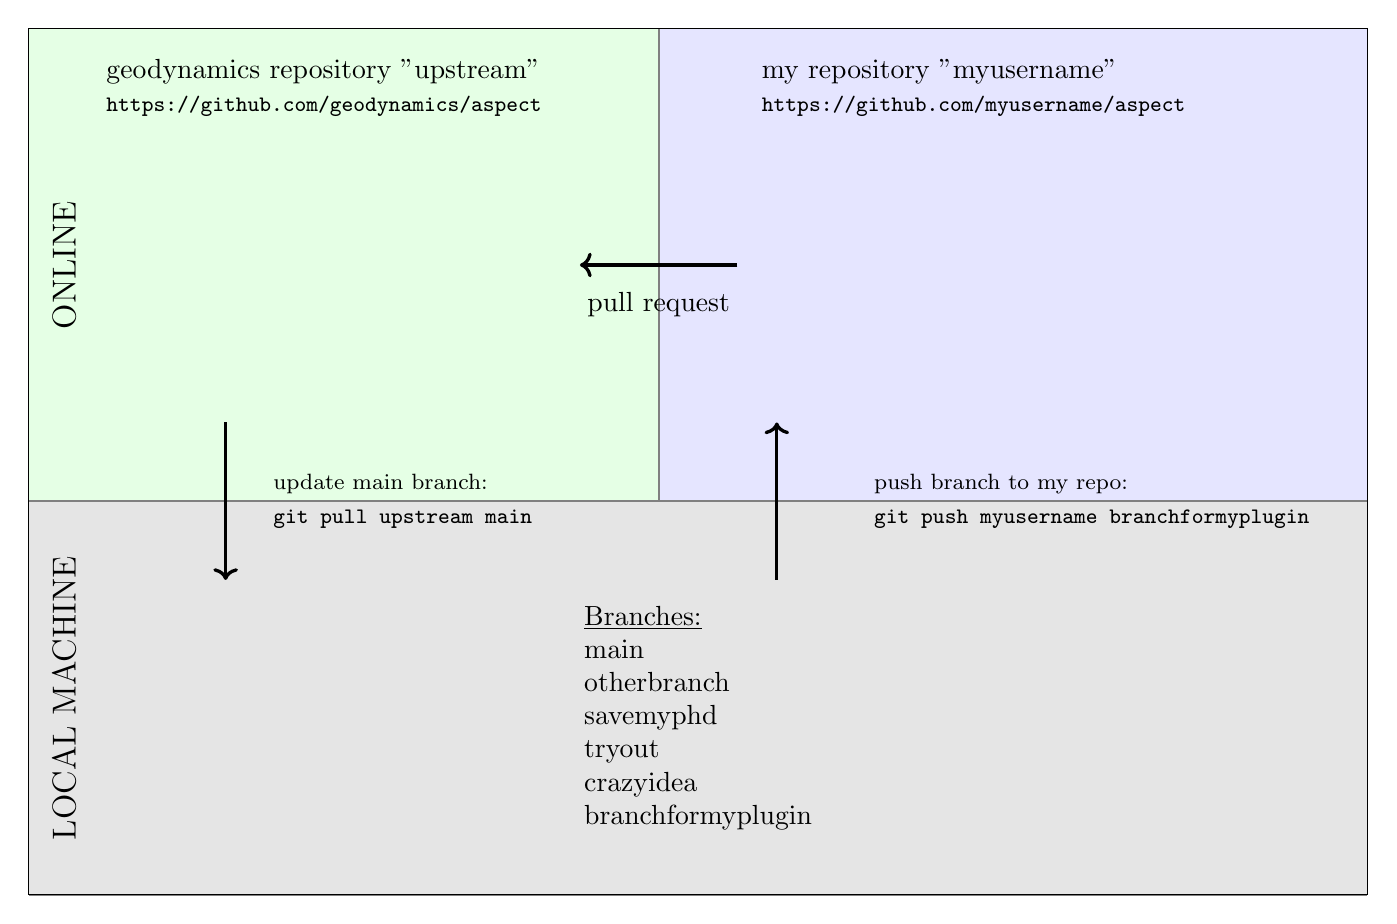
\begin{tikzpicture}
\draw[step=0.5cm,gray,very thin] (0,0) grid (17,11); %background grid

\draw[fill=gray!20] (0,0) rectangle (17,5);
\draw[fill=green!10] (0,5) rectangle (8,11); 
\draw[fill=blue!10] (8,5) rectangle (17,11); 

\draw[gray,thick] (0,5) -- (17,5); %horizontal line
\draw[gray,thick] (8,5) -- (8,11); %vertical line
%\draw[thick] (12,5) -- (12,11); %vertical line

\node[align=left] at (3.75,10.25) {geodynamics repository "upstream"\\ \footnotesize \verb"https://github.com/geodynamics/aspect"};

\node[align=left] at (12,10.25) {my repository "myusername"\\ \footnotesize \verb"https://github.com/myusername/aspect"};

\node[rotate=90] at (0.45,8) {\large ONLINE};
\node[rotate=90] at (0.45,2.5) {\large LOCAL MACHINE};

\draw[->,very thick] (9,8) -- (7,8);
\node[align=left] at (8,7.5) {pull request};

\node[align=left] at (8.5,2.25) {\underline{Branches:}\\main\\otherbranch\\savemyphd\\tryout\\crazyidea\\branchformyplugin};

\draw[->,very thick] (2.5,6) -- (2.5,4);
\node[align=left] at (4.75,5) {\footnotesize update main branch:\\
\footnotesize \verb"git pull upstream main"};

\draw[->,very thick] (9.5,4) -- (9.5,6);
\node[align=left] at (13.5,5) {\footnotesize push branch to my repo:\\
\footnotesize \verb"git push myusername branchformyplugin"};

\end{tikzpicture}


%..............................................
\paragraph{Very concretely, if you wish to contribute:} 

Let us assume that you have found a typo in the file ``physics.cc'' and you wish to 
fix this problem. 

\begin{enumerate}
\item
If this is the very first time you use git, the following instruction is not needed. If not, 
make sure that your terminal points at your main branch:
\verb"$ git checkout main"

\item
Then, make sure you update your local version:
\verb"$ git pull upstream main" 
and also update your own repo online:
\verb"$ git push username main"

\item
Create a new branch with a self explanatory name:
\verb"$ git branch fix_typo"
Then do \verb"$ git branch" to see all your branches. The one that is coloured is 
the active branch. In order to switch to this new branch, do 
\verb"$ git checkout fix_typo". Redo \verb"$ git branch" to verify that 
the branch 'fix\_typo' is highlighted.

\item
Edit the file physics.cc, correct the typo, save and exit. 
Do \verb"$ git status" and you should see the filename highlighted next to 'modified'. 

\item before we go any further, we need to run the indenting script with astyle. 
In the build directory run \verb'$ make indent'.
Note that you need a specific version of astyle, see \url{https://github.com/geodynamics/aspect/wiki/Indenting-code-and-installing-the-correct-version-of-astyle} 

\item add a changelog entry in doc/modules/changes. Look at the entries and find the one that resembles your contribution the most. Use it to 
write your entry.

\item If this is the only modification you wish to communicate, you then need to add and commit 
it as follows:
\begin{verbatim}
$ git add physics.cc
\end{verbatim}
If you do \verb'$ git status' again, the file should have changed colour. 
Then do
\begin{verbatim}
$ git commit -m "message"
\end{verbatim}
where 'message' is a very short description of the modification (e.g. 'I fixed a typo').

\item We now need to bring this modification online 
\begin{verbatim}
$ git push myusername fix_typo
\end{verbatim}

\item You are nearly done. The last step takes place on github.com: when you log onto 
your own github fieldstone page, you should see a large green rectangle "Compare and pull request".
Click on this button, follow the instructions.

\item a new page opens, entitled "Open a pull request" (PR). If necessary, add a detailed description of 
the pull request (this makes sense when you contribute a piece of code, or a whole new section, etc ...).
Later you will be able to review the requested changes at the bottom. In the end, simply click "Create pull request".

\item Once you have done so, \aspect developers will then review it. 
If they have no comment, the PR will be accepted and your modification will 
then be incorporated in the main repo. If they have comments, you will be notified via github and a 
back-and-forth discussion will ensue until the PR is accepted. 

\item if the reviewers have comments. Edit/change your file(s). 
Then add these (\verb'git add ...'), and commit again (\verb'git commit -m "msg"')
and push as before. \\
OR: better: \\
\verb'git commit --amend -a' so that you don't have to squash/fixup afterwards



\item After the PR has been accepted, the branch is no longer needed. Switch back to your local main branch:
\$ \verb"git checkout main ".
Update your local main and online repo (see step \# 2) and then delete the no-longer-needed 
branch as follows:
\begin{verbatim}
$ git branch -d fix_typo
\end{verbatim}
\end{enumerate}

-----------------------------------

If there is a pb with your PR and u need to rebase. For example if your 2 PRs modify the same line (say for example reference.bib - 
in that case better spread your changes to different locations in the reference.bib)

\begin{itemize}
\item carry out modifications as required by reviewers
\item \verb'git add' files, and \verb' git commit'
\item \verb'git checkout main'
\item \verb'git branch', make sure you are indeed back on main
\item \verb'git pull upstream main'. depending how much happened in the last hours/days it will display a bunch of files/updates
\item \verb'git checkout my_branch'
\item \verb'git rebase main'. Follow instructions, resolve conflicts in indicated files. 
\verb'git add problematic_file'. 
Finish with \verb'git rebase --continue'. 
\item \verb'git push -f cedrict my_branch'
\end{itemize}

To configure the editor used by git (do it once):
\begin{verbatim}
git config --global core.editor "vim"
\end{verbatim}


git stash 
git stash pop


git log


\newpage
how to squash/fixup:

git rebase -i main $->$  

A similar window as this will open:

\begin{center}
\includegraphics[width=10cm]{images/github/aaa}
\end{center}

Since we wish to squash (or rather fixup!) we do:

\begin{center}
\includegraphics[width=10cm]{images/github/bbb}
\end{center}

save and exit

do git diff

\newpage




%%%%%%%%%%%%%%%%%%%%%%%%%%%%%%%%%%%%%%%%%%%%%%%%%%%%%%%%%%%%%%%%%%%%%%%%%%%%%%%%%%%%%%%%%%%%%%%%%
\newpage

\subsection{Contributing a cookbook in \aspect}

\begin{enumerate}
\item Download/update/install \aspect 
\item In the cookbooks folder, create a new folder: \verb'$ mkdir my_cool_setup'
\item In this folder, place your .prm file, say my\_cool\_setup.prm
\item Make sure your .prm file is clean, commented, and contains a header with a concise
description of what the experiment is, and/or in which publication it originates.
\item In the folder, create a new folder:  \verb'$ mkdir doc'
\item In this folder create the file my\_cool\_setup.md file which contains the 
text for the cookbook. Look at other cookbooks md files for examples of how 
to include a figure, an equation, cite publications, etc ...
\item Place in this same folder all figures pertaining 
to the cookbook entry in the manual. 
\item go to \verb'/doc/sphinx/user/cookbooks/' and add your cookbook to the list in 
(for example) \verb'geophysical-setups.md'
\item if you with to cite publications, add them to \verb'/doc/sphinx/references.bib'
\item In order to generate the manual, go to /doc/sphinx and do \verb"$ make html"

\item if you wish to re-generate the part of the manual that comes from the documentation
of .cc files, then got to \verb'\build' and \verb'make' the code, then do in \verb'/doc/': 
\begin{verbatim}
./update_parameters.sh /home/absolute/path/aspect/build/aspect
\end{verbatim}
and then do \verb'make html'. If you re-modify the .cc file, you need to redo all 3 steps.

\item If there is no error, you should be able to open the file \verb'/doc/sphinx/\_build/html/index.html'
with firefox
\item if the referencing of the figures does not work correctly, simply do 
\verb'make clean' and then make html again.
\item before you make a pull request, make sure you run \verb'make indent'
\end{enumerate}



%%%%%%%%%%%%%%%%%%%%%%%%%%%%%%%%%%%%%%%%%%%%%%%%%%%%%%%%%%%%%%%%%%%%%%%%%%%%%%%%%%%%%%%%%%%%%%%%%
%%%%%%%%%%%%%%%%%%%%%%%%%%%%%%%%%%%%%%%%%%%%%%%%%%%%%%%%%%%%%%%%%%%%%%%%%%%%%%%%%%%%%%%%%%%%%%%%%
%%%%%%%%%%%%%%%%%%%%%%%%%%%%%%%%%%%%%%%%%%%%%%%%%%%%%%%%%%%%%%%%%%%%%%%%%%%%%%%%%%%%%%%%%%%%%%%%%
\newpage
\subsection{Contributing to fieldstone}

\begin{mdframed}[backgroundcolor=red!5]
This appendix was contributed by E. van der Wiel.
\end{mdframed}


\begin{enumerate}
\item make sure that you  have an account on GitHub (say, \verb"https://github.com/myusername") 
and carry out a proper setup on your local computer as follows:\\
\$ \verb'git config --global user.name "firstname lastname" '\\
\$ \verb'git config --global user.email your@email'

\item On github.com, fork the official fieldstone 
repository to your repository:\\
go to \verb"https://github.com/cedrict/fieldstone" 
and click on the 'fork' button on the upper right corner of the screen.
\item On your machine, in a terminal, clone your repository with \\
\$ \verb"git clone git@github.com:myusername/fieldstone.git". This is now your main\footnote{also 'master', although this term should not be used anymore} branch.

\item On your machine, find your security key \footnote{
Note that you can create a public key as follows: 
{\tt https://help.github.com/articles/generating-ssh-keys/}}
 with \$ \verb"less ~/.ssh/id_dsa.pub" and copy this into github.com 
so you can push to your repository. See \url{https://help.github.com/en/articles/connecting-to-github-with-ssh} on how to configure github with ssh support (no more login/password to type -- if you have cloned the repository wish ssh, not html).
Please also check the instructions at \url{https://help.github.com/en/articles/connecting-to-github-with-ssh}.  
 
\item create a remote of your (online) repository\\
\verb"git remote add origin git@github.com:myusername/fieldstone.git"
and in order to avoid potential confusion later on, we shall rename our github repo as follows:\\
\$ \verb"git remote rename origin myusername" 

\item Also create a remote of the official version with\\
\$ \verb"git remote add upstream https://github.com/cedrict/fieldstone"

\end{enumerate}


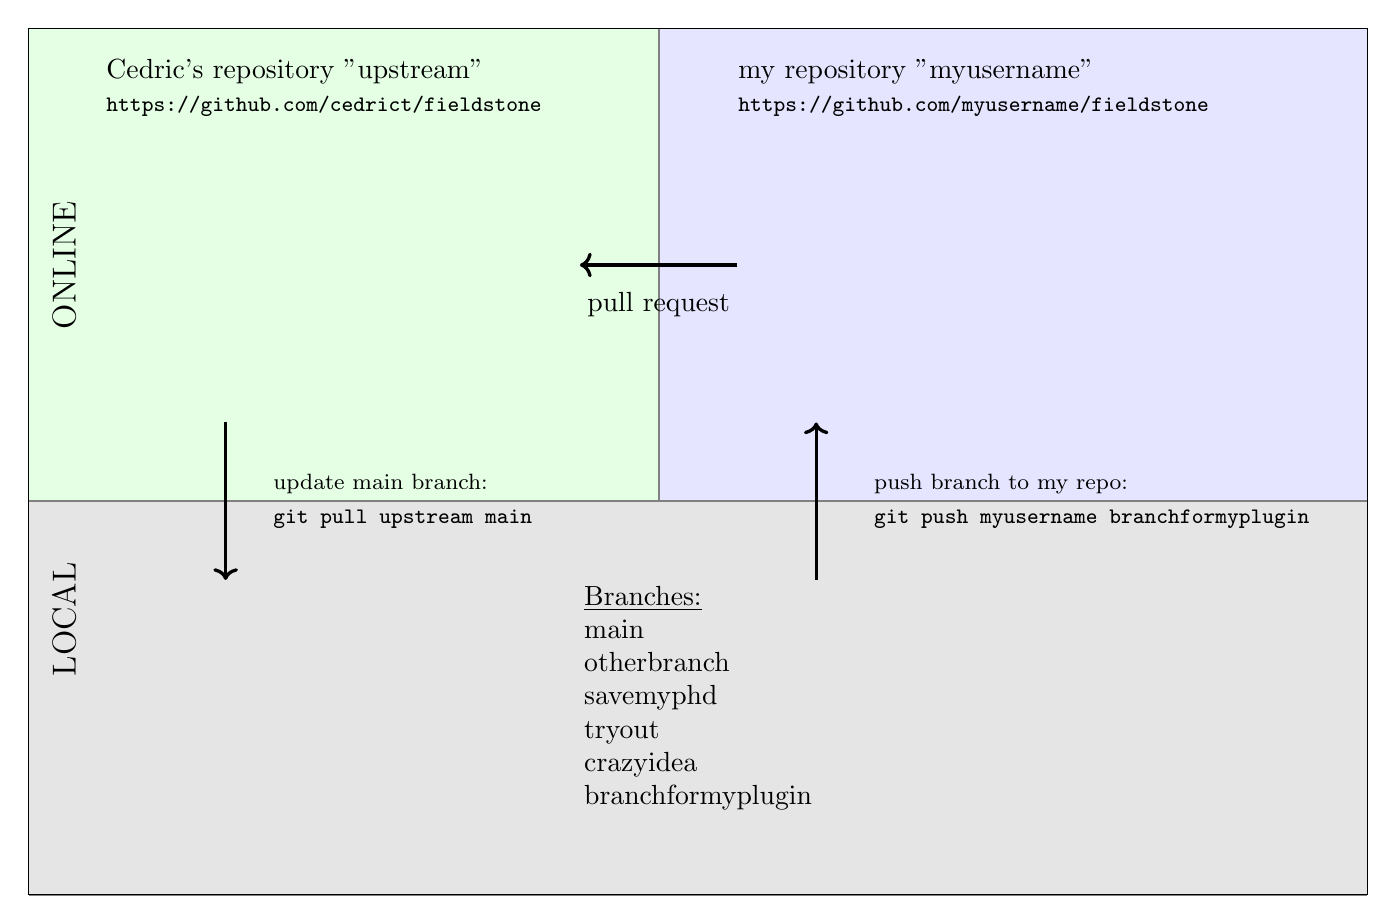
\begin{tikzpicture}
\draw[step=0.5cm,gray,very thin] (0,0) grid (17,11); %background grid

\draw[fill=gray!20] (0,0) rectangle (17,5);
\draw[fill=green!10] (0,5) rectangle (8,11); 
\draw[fill=blue!10] (8,5) rectangle (17,11); 

\draw[gray,thick] (0,5) -- (17,5); %horizontal line
\draw[gray,thick] (8,5) -- (8,11); %vertical line
%\draw[thick] (12,5) -- (12,11); %vertical line

\node[align=left] at (3.75,10.25) {Cedric's repository "upstream"\\ \footnotesize \verb"https://github.com/cedrict/fieldstone"};

\node[align=left] at (12,10.25) {my repository "myusername"\\ \footnotesize \verb"https://github.com/myusername/fieldstone"};

\node[rotate=90] at (0.45,8) {\large ONLINE};
\node[rotate=90] at (0.45,3.5) {\large LOCAL};

\draw[->,very thick] (9,8) -- (7,8);
\node[align=left] at (8,7.5) {pull request};

\node[align=left] at (8.5,2.5) {\underline{Branches:}\\main\\otherbranch\\savemyphd\\tryout\\crazyidea\\branchformyplugin};

\draw[->,very thick] (2.5,6) -- (2.5,4);
\node[align=left] at (4.75,5) {\footnotesize update main branch:\\
\footnotesize \verb"git pull upstream main"};

\draw[->,very thick] (10,4) -- (10,6);
\node[align=left] at (13.5,5) {\footnotesize push branch to my repo:\\
\footnotesize \verb"git push myusername branchformyplugin"};

\end{tikzpicture}


%..............................................
\paragraph{Very concretely, if you wish to contribute:} 

Let us assume that you have found a typo in the file "physics.tex" and you wish to 
report the problem to me. The easiest way is to write me an email with the nature of the 
problem and the proposed fix. Although I will be grateful for your contribution,
this approach can be improved upon by using git's "pull request" command. 



\begin{enumerate}
\item
If this is the very first time you use git, the following instruction is not needed. If not, 
make sure that your terminal points at your main branch:
\verb"$ git checkout master"

\item
Then, make sure you update your local version:
\verb"$ git pull upstream master" 
and also update your own repo online:
\verb"$ git push"

\item
Create a new branch with a self explanatory name:
\verb"$ git branch fix_typo"
Then do \$ \verb"git branch" to see all your branches. The one that is coloured is 
the active branch. In order to switch to this new branch, do 
\verb"$ git checkout fix_typo". Redo \verb"$ git branch" to verify that 
the branch 'fix\_typo' is highlighted.


\item
Edit the file and correct the typo, save and exit. 
Do \verb"$ git status" and you should see the filename highlighted next to 'modified'. 

\item If this is the only modification you wish to communicate, you then need to add and commit 
it as follows:
\begin{verbatim}
$ git add physics.tex
\end{verbatim}
If you do git status again, the file should have changed colour (?). 
Then do
\begin{verbatim}
$ git commit -m "message"
\end{verbatim}
where 'message' is a very short description of the modification (e.g. 'I fixed a typo').

\item We now need to bring this modification online 
\begin{verbatim}
$ git push myusername fix_typo
\end{verbatim}

\item You are nearly done. The last step takes place on github.com: when you log onto 
your own github fieldstone page, you should see a large green rectangle "Compare and pull request".
Click on this button.

\item a new page opens, entitled "Open a pull request". If necessary, add a detailed description of 
the pull request (this makes sense when you contribute a piece of code, or a whole new section, etc ...).
You can review the requested changes at the bottom. In the end, simply click "Create pull request".

\item Once you have done so, I will receive an email which notifies me of the pull request. I will 
then review it. If I have no comment, I will accept the PR and your modification will 
then be incorporated in the master repo. If I have comments, you will be notified via github and a 
back-and-forth discussion will ensue until I accept the PR. 

\item After the PR has been accepted, the branch is no longer needed. Switch back to your local master branch:
\$ \verb"git checkout master ".
Update your local master and online repo (see step \# 2) and then delete the no-longer-needed 
branch as follows:
\begin{verbatim}
$ git branch -d fix_typo
\end{verbatim}
\end{enumerate}

\newpage
\begin{center}
\includegraphics[width=9cm]{images/github/1}\\
\includegraphics[width=9cm]{images/github/2}\\
\includegraphics[width=9cm]{images/github/3}\\
\includegraphics[width=9cm]{images/github/4}\\
\includegraphics[width=9cm]{images/github/6}\\
{\captionfont Screen captures of the procedure described above as 
carried out by E. van der Wiel on his Apple laptop.}
\end{center}
















































\newpage
%%%%%%%%%%%%%%%%%%%%%%%%%%%%%%%%%%%%%%%%%%%%%%%%%%%%%%%%%%%%%%%%%%%%%%%%%%%%%%%%%%%%%%%%%%%%%%%%%%%%%%%%%
In what follows we summarize the most important commands one should and remember while working with github. 
After creating an account one can 'fork' a repository (repo) in the online environment. This repository is a 
copy from the master directory of the developer and should not be used to adapt or change, as changes from the developer (updates) should be obtained in this 'fork', or as it could also be called; your master branch. 
  
In order to be able to work within a repository, for instance, to run and compile different programs, you should have you own branch of the repository in which YOU CAN make changes. The following commands should be used to make, copy and publish your own version of the repo to your local device and the online github environment.

\begin{center}
\begin{tabular}{p{6cm}|p{9cm}}
\textbf{command} &  \textbf{what it does} \\
\hline
  git branch & shows all branches of your repository and highlights the one you're in. \\
  git checkout -b \textless my\_own\_branch\textgreater & This makes your own branch called "my\_own\_branch". \\
  git push origin \textless my\_own\_branch\textgreater & This pushes your own, local, branch to as a second branch in the online repo of github. \\
  git checkout \textless name\textgreater & changing the branch your working in (e.g. master or my\_own\_branch). Or replace the name with a hyphen to switch to the last branch.\\
  git branch -d \textless my\_own\_branch\textgreater & Delete your local branch. \\
  \end{tabular}
\end{center}

  The following commands should be used in order to update your own local branches from updates made by somewhere else (upstream/master is the main repository). One should do this for the local master branch and, where possible as well for the different local branches you have committed changes to already. 

  
\begin{center}
\begin{tabular}{p{6cm}|p{9cm}}
\textbf{command} &  \textbf{what it does} \\
\hline
git checkout master & To make sure you are in the right branch \\
  git fetch upstream & to fetch updates from upstream repositories to you own local branch (e.g. to update your master branch. \\
  git merge upstream/master & Command to update the branch with the fethched repo from 'upstream'. \\
  git push origin master & To level your own online repository again with the one on your local drive (and thus the one upstream). \\
  git checkout \textless my\_own\_branch\textgreater & To switch to your own adapted branch of the repo. \\
  git merge master & Used from another branch working directory to combine the new released version of the master repo with the one where all your own changes are put. -\textgreater Then git finds all conflicts in different files which you need to resolve. \\
  git add . & This adds the resolved issues in your own local branch (not master). After which you are able to commit and push your changes back to the online respository. 
\end{tabular}
\end{center}


While you are working in your own branch you can change, add or delete files in any amount you want. However, always check whether your changes do not inflict the outcome of for instance your code. And when uploading from your terminal: if you commit and then push from master branch your changes will automatically be inserted in the online version of your master branch, when done from another branch it will be shown as a pull request towards your master branch. This request can than, for instance be forwarded to the main repo.\\

\begin{center}
\begin{tabular}{p{6cm}|p{9cm}}
\textbf{command} &  \textbf{what it does} \\
\hline
  git commit -a & This will send your changes/updates from your branch as a commit to your own local branch. \\
  git push origin \textless changes\textgreater & To update the remote repository (on Github) from you local repository (in this case the 'changes' branch). (Actually upload the new version). Online one can then judge what to do with it. !! this is a pull request towards your own fork/local\_branch \\ 
  git status & Showing the status of your current branch; it shows which files are different between the master file and your adapted branch. \\
  git diff \textless changes\textgreater& This shows the exact differences between the different branches; one can simply ask for the difference between two branches when pwd in one branch ask for the other branch. \\ 
  git merge \textless my\_own\_branch\textgreater & When used from the master branch (or any other???) this accepts the changes made in your branch and puts them in your local(!) master branch. \\ 
  git pull origin master & if the main repository changes, one can pull the newest version towards it's own master file. While keeping your own branches alive with you own changes and vica versa: by running this command the origin/master (remote file) will be cloned and updated to the working branch you are in. \\
  git stash (apply) & ?? While updating your local branch, sometimes git wants to overrule your own changes, with this command you can 'stash' them to look at the differences later. ?? \\
\end{tabular}
\end{center}

 %%%%%%%%%%%%%%%%%%%%%%%%%%%%%%%%%%%%%%%
\chapter{Writing a report as homework \label{app:grading}} \begin{flushright} {\tiny {\color{gray} app\_grading.tex}} \end{flushright}
%~~~~~~~~~~~~~~~~~~~~~~~~~~~~~~~~~~~~~~~~~~~~~~~~~~~~~~~~~~~~~~~~~~~~~~~~~~~~~~~~~~~~~~~~~~~~~~~~~~


\begin{itemize}
\item 
The document should contain your full name and student number on the first page. 
\item 
The file should be a pdf which name contains your family name
\item 
Layout: is the document visually pleasing? Is it well structured? 
\item Is there a complete bibliography (when applicable)?
\item Does the structure follows this: Introduction - Methods - Results - Discussion - Conclusion - Appendix ?
\item 
Figures: Are they properly numbered? captioned? all figures must be referenced in the text. 
Are they of good enough quality (no visible pixels)? are they readable? are all axis labelled?
\item 
Text: Overall quality of the language. Are there still typos? Do all sentence make sense?
\item if you wish to show lines of code, use verbatim or lstlisting\footnote{\url{https://en.wikibooks.org/wiki/LaTeX/Source_Code_Listings}} 
\item 
Discussion: are the results properly discussed, analyzed? are potential problems, errors, limitations discussed?
\item 
Conclusion: Are the findings/results summarized and generalized?
\end{itemize}

\begin{center}
\begin{tabular}{cc}
\hline
No & Yes \\
\hline
\hline
$6.67*10^{-11}$ & $6.67 \times 10^{-11}$ \\
$kg/m^3$ &  kg/m$^{3}$ or kg.m$^{-3}$\\
1x1 & 1$\times$1\\
$cos$ & $\cos$\\
docx file & pdf file \\
'if you do this'& passive form \\ 
\hline
\end{tabular}
\end{center}




%.....................................
\par\noindent\rule{\textwidth}{0.4pt}
\begin{center}
\includegraphics[width=10cm]{images/grading/grey}\\
No grey background
\end{center}


%.....................................
\par\noindent\rule{\textwidth}{0.4pt}
\begin{center}
\includegraphics[width=10cm]{images/grading/numbers}\\
No lists/arrays with numbers
\end{center}

%.....................................
\par\noindent\rule{\textwidth}{0.4pt}
\begin{center}
\includegraphics[width=10cm]{images/grading/arrows2}\\
Too many arrows\\
\includegraphics[width=9cm]{images/grading/arrows1}\\
Poor choice of arrow colour
\end{center}

%.....................................
\par\noindent\rule{\textwidth}{0.4pt}
\begin{center}
\includegraphics[width=8cm]{images/grading/pixels1}
\includegraphics[width=7cm]{images/grading/pixels2}\\
Be careful about how you export your figures. These are unreadable.
\end{center}
 
%.....................................
\par\noindent\rule{\textwidth}{0.4pt}
\begin{center}
\includegraphics[width=8cm]{images/grading/eqs1}\\
Parenthesis too small
\end{center}

%.....................................
\par\noindent\rule{\textwidth}{0.4pt}
\begin{center}
\includegraphics[width=9cm]{images/grading/eqs2}\\
1.6E+10 is not acceptable. Replace by $1.6\cdot 10^{10}$
\end{center}

%.....................................
\par\noindent\rule{\textwidth}{0.4pt}
\begin{center}
\includegraphics[width=7cm]{images/grading/eqs3}\\
Equation number is too close to the equation itself. Use labels, 
do not number equations by hand.
\end{center}

%.....................................
\par\noindent\rule{\textwidth}{0.4pt}
\begin{center}
\includegraphics[width=9cm]{images/grading/eqs4}\\
Formatting of both axis lead to unreadable figure.
\end{center}

%.....................................
\par\noindent\rule{\textwidth}{0.4pt}
\begin{center}
\includegraphics[width=9cm]{images/grading/eqs5}\\
In \LaTeX{}  use \verb!\sum\limits!
\end{center}

%.....................................
\par\noindent\rule{\textwidth}{0.4pt}
\begin{center}
\includegraphics[width=9cm]{images/grading/eqs6}\\
Are so many digits necessary?
\end{center}

%.....................................
\par\noindent\rule{\textwidth}{0.4pt}
\begin{center}
\includegraphics[width=12cm]{images/grading/width}\\
use \verb!\usepackage[cm]{fullpage}! to allow for wider text.
\end{center}

%.....................................
\par\noindent\rule{\textwidth}{0.4pt}
\begin{center}
\includegraphics[width=10cm]{images/grading/figs1}\\
This figure style is to be avoided. Simply use dots and/or lines.
\end{center}

%.....................................
\par\noindent\rule{\textwidth}{0.4pt}
\begin{center}
\includegraphics[width=8cm]{images/grading/figs2}
\end{center}

%.....................................
\par\noindent\rule{\textwidth}{0.4pt}
\begin{center}
\includegraphics[width=6cm]{images/grading/loglogpb}\\
Here Ra and Nu are plotted in log-log scale, not log(Ra) and log(Nu).
\end{center}

%.....................................
\par\noindent\rule{\textwidth}{0.4pt}
\begin{center}
\includegraphics[width=10cm]{images/grading/dots}\\
The dots at the beginning and end of the lines are not necessary.
\end{center}

%.....................................
\par\noindent\rule{\textwidth}{0.4pt}
\begin{center}
\includegraphics[width=11cm]{images/grading/you}\\
Never {\it never} use 'you'. 
\end{center}

%.....................................
\par\noindent\rule{\textwidth}{0.4pt}
\begin{center}
\includegraphics[width=10cm]{images/grading/cross}\\
Do not use 'X' but $\times$ (\verb|\times|).
\end{center}




%------------------------------------------------------------
\subsection{Computational Geodynamics Report}

All the comments above apply, with additional instructions:
\begin{itemize}
\item report should be in \LaTeX 
\item The document should contain your full name and student number on the first page. 
\item The report file should be a pdf which name contains your family name
\item not more than 25 pages. If more, use appendices wisely.
\item document should be structured in two main parts: FDM and FEM.
\item no equations unless necessary to the discussion (still mention the equation that 
you are solving but refer to an external document/article/book for example).
\item use lstlisting package to include code
\item use {\verb| \usepackage[cm]{fullpage} |} to format your document
\item all codes either in appendix or in zip file (bearing your name).
\item a decent introduction (half page to one page) which links the topic of this course to geosciences.
\item discussion of results (stability, convergence, influence of resolution, remarks of all kinds).
\item if you did not succeed in doing a particular exercise, please explain what you think the problem is, 
how you know it is not working, etc ...
\item think about colormaps, image compression
\item DEADLINE: July 16th, 2023, 23:59 
\end{itemize}


I will use this table to grade your reports:

\vspace{2cm}


\begin{tabular}{|p{5cm}|p{.35cm}|p{.35cm}|p{.35cm}|p{.35cm}|p{.35cm}|p{.35cm}|p{.35cm}|p{.35cm}|p{.35cm}|p{.35cm}|p{.35cm}|p{.35cm}|p{.35cm}|p{.35cm}|p{.35cm}|}
&&&&&&&&&&&&&&& \\
\hline
title, names, student nb &&&&&&&&&&&&&&& \\\hline
\LaTeX ? &&&&&&&&&&&&&&& \\\hline
document layout &&&&&&&&&&&&&&& \\\hline
equations look &&&&&&&&&&&&&&& \\\hline
equations numbered  &&&&&&&&&&&&&&& \\\hline
use of equations &&&&&&&&&&&&&&& \\\hline
figs: caption &&&&&&&&&&&&&&& \\\hline
figs: pixels? &&&&&&&&&&&&&&& \\\hline
figs: correct? &&&&&&&&&&&&&&& \\\hline
English grammar &&&&&&&&&&&&&&& \\\hline
Typos 
Introduction &&&&&&&&&&&&&&& \\\hline
methods/results &&&&&&&&&&&&&&& \\\hline
Discussion/Conclusion  &&&&&&&&&&&&&&& \\\hline
Extra work? &&&&&&&&&&&&&&& \\\hline
Bibliography &&&&&&&&&&&&&&& \\\hline
code layout &&&&&&&&&&&&&&& \\\hline 
code style &&&&&&&&&&&&&&& \\\hline
code accuracy &&&&&&&&&&&&&&& \\\hline
\end{tabular}

 %%%%%%%%%%%%%%%%%%%%
\chapter{Analytical expressions for $\G_{el}$} \label{app:Gel} 


The elemental matrix $\G_{el}$ is given by (see Section~\ref{sec:mixed}):

\[
\G_{el} = -\int_{\Omega_e} {\bm B}^T \cdot {\bm N} d\Omega
= -\int_{\Omega_e}
\left(
\begin{array}{ccc}
\partial_x \bN_1^\upnu & 0 & \partial_y \bN_1^\upnu \\
0 & \partial_y \bN_1^\upnu & \partial_x \bN_1^\upnu \\
\partial_x \bN_2^\upnu & 0 & \partial_y \bN_2^\upnu \\
0 & \partial_y \bN_2^\upnu & \partial_x \bN_2^\upnu \\
\dots & \dots & \dots \\
\dots & \dots & \dots \\
\partial_x \bN_{m_\upnu}^\upnu & 0 & \partial_y \bN_{m_\upnu}^\upnu \\
0 & \partial_y \bN_{m_\upnu}^\upnu & \partial_x \bN_{m_\upnu}^\upnu 
\end{array}
\right)
\cdot
\left(
\begin{array}{cccc}
\bN_1^p & \bN_2^p & \dots & \bN_{m_p}^p \\ 
\bN_1^p & \bN_2^p & \dots & \bN_{m_p}^p \\ 
0 & 0 & \dots & 0
\end{array}
\right)
d\Omega
\]

In what follows I set out to compute this elemental matrix for the reference element $[-1:1]\times[-1:1]$.
All of the integrals were computed with WolframAlpha\footnote{\url{https://www.wolframalpha.com/}} 
since it allowed me to copy-paste
the \LaTeX code directly into the website prompt area and obtain the value of these integrals.


%-------------------------------------------------------------------
\subsection{$Q_1\times P_0$ element (2d case)}

For this element, $m_\upnu=4$ and $m_p=1$ so $\G_{el}$ is
a $8\times 1$ matrix:
\[
\G_{el} = -\int_{\Omega_e} {\bm B}^T \cdot {\bm N} d\Omega
= -\int_{\Omega_e}
\left(
\begin{array}{ccc}
\partial_r \bN_1^\upnu & 0 & \partial_s \bN_1^\upnu \\
0 & \partial_s \bN_1^\upnu & \partial_r \bN_1^\upnu \\
\partial_r \bN_2^\upnu & 0 & \partial_s \bN_2^\upnu \\
0 & \partial_s \bN_2^\upnu & \partial_r \bN_2^\upnu \\
\partial_r \bN_3^\upnu & 0 & \partial_s \bN_3^\upnu \\
0 & \partial_s \bN_3^\upnu & \partial_r \bN_3^\upnu \\
\partial_r \bN_4^\upnu & 0 & \partial_s \bN_4^\upnu \\
0 & \partial_s \bN_4^\upnu & \partial_r \bN_4^\upnu 
\end{array}
\right)
\cdot
\left(
\begin{array}{c}
\bN_1^p  \\ 
\bN_1^p  \\ 
0 
\end{array}
\right)
d\Omega
\]
also, since $\bN_1^p(r,s)=1$ then
\[
\G_{el} = -\int_{\Omega_e} {\bm B}^T \cdot {\bm N} d\Omega
= -\int_{\Omega_e}
\left(
\begin{array}{ccc}
\partial_r \bN_1^\upnu  \\
\partial_s \bN_1^\upnu  \\
\partial_r \bN_2^\upnu  \\
\partial_s \bN_2^\upnu  \\
\partial_r \bN_3^\upnu  \\
\partial_s \bN_3^\upnu  \\
\partial_r \bN_4^\upnu  \\
\partial_s \bN_4^\upnu  
\end{array}
\right)
d\Omega
=
\left(
\begin{array}{c}
 1\\
 1\\
-1\\
 1\\
-1\\
-1\\
 1\\
-1
\end{array}
\right)
\]

A macro element made of a single element makes no sense since if velocity
is prescribed on all sides there is not a single velocity dof left.

We then consider the following macro-element:

\begin{verbatim}
velocity      pressure
7====8====9   .====.====.
|    |    |   |  3 |  4 |
4====5====6   .====.====.   NV=9
|    |    |   |  1 |  2 |   
1====2====3   .====.====.   NP=4
\end{verbatim}


The assembled $\G$ matrix is then $18 \times 4$:
\[
\G = 
\left(
\begin{array}{cccc}
  1  &   0 &   0 &   0  \\ 
  1  &   0 &   0 &   0  \\ 
 -1  &   1 &   0 &   0  \\ 
  1  &   1 &   0 &   0  \\ 
  0  &  -1 &   0 &   0  \\ 
  0  &   1 &   0 &   0  \\ 
  1  &   0 &   1 &   0  \\ 
 -1  &   0 &   1 &   0  \\ 
 -1  &   1 &  -1 &   1  \\ 
 -1  &  -1 &   1 &   1  \\ 
  0  &  -1 &   0 &  -1  \\ 
  0  &  -1 &   0 &   1  \\ 
  0  &   0 &   1 &   0  \\ 
  0  &   0 &  -1 &   0  \\ 
  0  &   0 &  -1 &   1  \\ 
  0  &   0 &  -1 &  -1  \\ 
  0  &   0 &   0 &  -1  \\ 
  0  &   0 &   0 &  -1  
\end{array}
\right)
\]
After applying boundary conditions on nodes 1,2,3,4,6,7,8,9:

\[
\G = 
\left(
\begin{array}{cccc}
  0  &   0 &   0 &   0  \\ 
  0  &   0 &   0 &   0  \\ 
  0  &   0 &   0 &   0  \\ 
  0  &   0 &   0 &   0  \\ 
  0  &   0 &   0 &   0  \\ 
  0  &   0 &   0 &   0  \\ 
  0  &   0 &   0 &   0  \\ 
  0  &   0 &   0 &   0  \\ 
 -1  &   1 &  -1 &   1  \\ 
 -1  &  -1 &   1 &   1  \\ 
  0  &   0 &   0 &   0  \\ 
  0  &   0 &   0 &   0  \\ 
  0  &   0 &   0 &   0  \\ 
  0  &   0 &   0 &   0  \\ 
  0  &   0 &   0 &   0  \\ 
  0  &   0 &   0 &   0  \\ 
  0  &   0 &   0 &   0  \\ 
  0  &   0 &   0 &   0  
\end{array}
\right)
\]
or, defining $\tilde{\G}$ as the remaining matrix when the zero lines have been removed:
\[
\tilde{\G} = 
\left(
\begin{array}{cccc}
 -1  &   1 &  -1 &   1  \\ 
 -1  &  -1 &   1 &   1  
\end{array}
\right)
\]
The null space is of size two, spawn by the two vectors:
\begin{verbatim}
[[-0.1  0.7]
 [ 0.7  0.1]
 [ 0.7  0.1]
 [-0.1  0.7]]
\end{verbatim}

The means that we have two pressure solutions $\vec{\cal P}_{1,2}$ (and any linear combination of these 2) 
which are such that $\G\cdot\vec{\cal P}=\vec{0}$
while we would ideally want a single one, the constant vector.

In the book (which?) the authors proceed to show that any such macro-element
made of rectangles has a spurious mode.

See code {\tt python\_codes/Gel/macro\_element\_q1p0.py}


%-------------------------------------------------------------------
\subsection{$Q_1\times P_0$ element (3d case)}

For this element, $m_\upnu=8$ and $m_p=1$ so $\G_{el}$ is
a $3*8\times 1$ matrix:
\[
\G_{el} = -\int_{\Omega_e} {\bm B}^T \cdot {\bm N} d\Omega
= -\int_{\Omega_e}
\left(
\begin{array}{cccccc}
\partial_r \bN_1^\upnu & 0 & 0 & \partial_s \bN_1^\upnu  & \partial_t \bN_1^\upnu & 0 \\
0 & \partial_s \bN_1^\upnu  & 0 & \partial_r \bN_1^\upnu  & 0 & \partial_t \bN_1^\upnu \\
0 & 0 & \partial_t \bN_1^\upnu  & 0 & \partial_r \bN_1^\upnu  & \partial_s \bN_1^\upnu \\
\dots  & \dots & \dots  & \dots & \dots  & \dots \\
\dots  & \dots & \dots  & \dots & \dots  & \dots \\
\partial_r \bN_8^\upnu & 0 & 0 & \partial_s \bN_8^\upnu  & \partial_t \bN_8^\upnu & 0 \\
0 & \partial_s \bN_8^\upnu  & 0 & \partial_r \bN_8^\upnu  & 0 & \partial_t \bN_8^\upnu \\
0 & 0 & \partial_t \bN_8^\upnu  & 0 & \partial_r \bN_8^\upnu  & \partial_s \bN_8^\upnu 
\end{array}
\right)
\cdot
\left(
\begin{array}{c}
\bN_1^p  \\ 
\bN_1^p  \\ 
\bN_1^p  \\ 
0 \\
0 \\
0 
\end{array}
\right)
d\Omega
\]
also, since $\bN_1^p(r,s)=1$ then
\[
\G_{el} = -\int_{\Omega_e} {\bm B}^T \cdot {\bm N} d\Omega
= -\int_{\Omega_e}
\left(
\begin{array}{ccc}
\partial_r \bN_1^\upnu  \\
\partial_s \bN_1^\upnu  \\
\partial_t \bN_1^\upnu  \\
\partial_r \bN_2^\upnu  \\
\partial_s \bN_2^\upnu  \\
\partial_t \bN_2^\upnu  \\
\partial_r \bN_3^\upnu  \\
\partial_s \bN_3^\upnu  \\
\partial_t \bN_3^\upnu  \\
\partial_r \bN_4^\upnu  \\
\partial_s \bN_4^\upnu  \\
\partial_t \bN_4^\upnu  \\
\partial_r \bN_5^\upnu  \\
\partial_s \bN_5^\upnu  \\
\partial_t \bN_5^\upnu  \\
\partial_r \bN_6^\upnu  \\
\partial_s \bN_6^\upnu  \\
\partial_t \bN_6^\upnu  \\
\partial_r \bN_7^\upnu  \\
\partial_s \bN_7^\upnu  \\
\partial_t \bN_7^\upnu  \\
\partial_r \bN_8^\upnu  \\
\partial_s \bN_8^\upnu  \\
\partial_t \bN_8^\upnu  
\end{array}
\right)
d\Omega
=
-
\left(
\begin{array}{c}
\int_{-1}^{+1}\int_{-1}^{+1}\int_{-1}^{+1} \frac{1}{8}(-1)(1-s)(1-t) dr ds dt \\
\int_{-1}^{+1}\int_{-1}^{+1}\int_{-1}^{+1} \frac{1}{8}(1-r)(-1)(1-t) dr ds dt \\
\int_{-1}^{+1}\int_{-1}^{+1}\int_{-1}^{+1} \frac{1}{8}(1-r)(1-s)(-1) dr ds dt \\
\int_{-1}^{+1}\int_{-1}^{+1}\int_{-1}^{+1} \frac{1}{8}(+1)(1-s)(1-t) dr ds dt \\
\int_{-1}^{+1}\int_{-1}^{+1}\int_{-1}^{+1} \frac{1}{8}(1+r)(-1)(1-t) dr ds dt \\
\int_{-1}^{+1}\int_{-1}^{+1}\int_{-1}^{+1} \frac{1}{8}(1+r)(1-s)(-1) dr ds dt \\
\int_{-1}^{+1}\int_{-1}^{+1}\int_{-1}^{+1} \frac{1}{8}(+1)(1+s)(1-t) dr ds dt \\
\int_{-1}^{+1}\int_{-1}^{+1}\int_{-1}^{+1} \frac{1}{8}(1+r)(+1)(1-t) dr ds dt \\
\int_{-1}^{+1}\int_{-1}^{+1}\int_{-1}^{+1} \frac{1}{8}(1+r)(1+s)(-1) dr ds dt \\
\int_{-1}^{+1}\int_{-1}^{+1}\int_{-1}^{+1} \frac{1}{8}(-1)(1+s)(1-t) dr ds dt \\
\int_{-1}^{+1}\int_{-1}^{+1}\int_{-1}^{+1} \frac{1}{8}(1-r)(+1)(1-t) dr ds dt \\
\int_{-1}^{+1}\int_{-1}^{+1}\int_{-1}^{+1} \frac{1}{8}(1-r)(1+s)(-1) dr ds dt \\
\int_{-1}^{+1}\int_{-1}^{+1}\int_{-1}^{+1} \frac{1}{8}(-1)(1-s)(1+t) dr ds dt \\
\int_{-1}^{+1}\int_{-1}^{+1}\int_{-1}^{+1} \frac{1}{8}(1-r)(-1)(1+t) dr ds dt \\
\int_{-1}^{+1}\int_{-1}^{+1}\int_{-1}^{+1} \frac{1}{8}(1-r)(1-s)(+1) dr ds dt \\
\int_{-1}^{+1}\int_{-1}^{+1}\int_{-1}^{+1} \frac{1}{8}(+1)(1-s)(1+t) dr ds dt \\
\int_{-1}^{+1}\int_{-1}^{+1}\int_{-1}^{+1} \frac{1}{8}(1+r)(-1)(1+t) dr ds dt \\
\int_{-1}^{+1}\int_{-1}^{+1}\int_{-1}^{+1} \frac{1}{8}(1+r)(1-s)(+1) dr ds dt \\
\int_{-1}^{+1}\int_{-1}^{+1}\int_{-1}^{+1} \frac{1}{8}(+1)(1+s)(1+t) dr ds dt \\
\int_{-1}^{+1}\int_{-1}^{+1}\int_{-1}^{+1} \frac{1}{8}(1+r)(+1)(1+t) dr ds dt \\
\int_{-1}^{+1}\int_{-1}^{+1}\int_{-1}^{+1} \frac{1}{8}(1+r)(1+s)(+1) dr ds dt \\
\int_{-1}^{+1}\int_{-1}^{+1}\int_{-1}^{+1} \frac{1}{8}(-1)(1+s)(1+t) dr ds dt \\
\int_{-1}^{+1}\int_{-1}^{+1}\int_{-1}^{+1} \frac{1}{8}(1-r)(+1)(1+t) dr ds dt \\
\int_{-1}^{+1}\int_{-1}^{+1}\int_{-1}^{+1} \frac{1}{8}(1-r)(1+s)(+1) dr ds dt 
\end{array}
\right)
=
\left(
\begin{array}{c}
 1\\
 1\\
 1\\
-1\\
 1\\
 1\\
-1\\
-1\\
 1\\
 1\\
-1\\
 1\\
 1\\
 1\\
-1\\
-1\\
 1\\
-1\\
-1\\
-1\\
-1\\
 1\\
-1\\
-1
\end{array}
\right)
\]

If we consider a macro-element $2\times 2 \times 2$ of size $L_x=L_y=L_z=4$, apply velocity b.c on the all sides
we are left with
\[
\tilde{G} = 
\left(
\begin{array}{cccccccc}
-1 &-1 &-1 &-1 & 1 & 1 & 1 & 1\\
-1 &-1 & 1 & 1 &-1 &-1 & 1 & 1\\
-1 & 1 &-1 & 1 &-1 & 1 &-1 & 1
\end{array}
\right)
\]

Null space has dimension 5:
\begin{verbatim}
[[-0.35355339  0.35355339  0.35355339  0.35355339  0.35355339]
 [ 0.35355339 -0.35355339 -0.35355339  0.35355339  0.35355339]
 [ 0.35355339 -0.35355339  0.35355339 -0.35355339  0.35355339]
 [ 0.41990569  0.58009431  0.19336477  0.19336477 -0.19336477]
 [ 0.58009431  0.41990569 -0.19336477 -0.19336477  0.19336477]
 [ 0.19336477 -0.19336477  0.74028293  0.03317615 -0.03317615]
 [ 0.19336477 -0.19336477  0.03317615  0.74028293 -0.03317615]
 [-0.19336477  0.19336477 -0.03317615 -0.03317615  0.74028293]]
\end{verbatim}



%-------------------------------------------------------------------
\subsection{$Q_1\times Q_1$ element (2d case)}

For this element, $m_\upnu=4$ and $m_p=4$ so $\G_{el}$ is a $8\times 4$ matrix:

\begin{eqnarray}
\G_{el} 
&=& -\int_{\Omega_e} {\bm B}^T \cdot {\bm N} d\Omega \\
&=& -\int_{\Omega_e}
\left(
\begin{array}{ccc}
\partial_r \bN_1^\upnu & 0 & \partial_s \bN_1^\upnu \\
0 & \partial_s \bN_1^\upnu & \partial_r \bN_1^\upnu \\
\partial_r \bN_2^\upnu & 0 & \partial_s \bN_2^\upnu \\
0 & \partial_s \bN_2^\upnu & \partial_r \bN_2^\upnu \\
\partial_r \bN_3^\upnu & 0 & \partial_s \bN_3^\upnu \\
0 & \partial_s \bN_3^\upnu & \partial_r \bN_3^\upnu \\
\partial_r \bN_4^\upnu & 0 & \partial_s \bN_4^\upnu \\
0 & \partial_s \bN_4^\upnu & \partial_r \bN_4^\upnu \\
\end{array}
\right)
\cdot
\left(
\begin{array}{cccc}
\bN_1^p & \bN_2^p & \bN_3^p & \bN_{4}^p \\ 
\bN_1^p & \bN_2^p & \bN_3^p & \bN_{4}^p \\ 
0 & 0 & \dots & 0
\end{array}
\right)
d\Omega \\
&=&
-\int_{\Omega_e}
\left(
\begin{array}{cccc}
\bN_1^p\partial_r \bN_1^\upnu & \bN_2^p\partial_r \bN_1^\upnu & \bN_3^p\partial_r \bN_1^\upnu & \bN_4^p\partial_r \bN_1^\upnu \\
\bN_1^p\partial_s \bN_1^\upnu & \bN_2^p\partial_s \bN_1^\upnu & \bN_3^p\partial_s \bN_1^\upnu & \bN_4^p\partial_s \bN_1^\upnu \\
\bN_1^p\partial_r \bN_2^\upnu & \bN_2^p\partial_r \bN_2^\upnu & \bN_3^p\partial_r \bN_2^\upnu & \bN_4^p\partial_r \bN_2^\upnu \\
\bN_1^p\partial_s \bN_2^\upnu & \bN_2^p\partial_s \bN_2^\upnu & \bN_3^p\partial_s \bN_2^\upnu & \bN_4^p\partial_s \bN_2^\upnu \\
\bN_1^p\partial_r \bN_3^\upnu & \bN_2^p\partial_r \bN_3^\upnu & \bN_3^p\partial_r \bN_3^\upnu & \bN_4^p\partial_r \bN_3^\upnu \\
\bN_1^p\partial_s \bN_3^\upnu & \bN_2^p\partial_s \bN_3^\upnu & \bN_3^p\partial_s \bN_3^\upnu & \bN_4^p\partial_s \bN_3^\upnu \\
\bN_1^p\partial_r \bN_4^\upnu & \bN_2^p\partial_r \bN_4^\upnu & \bN_3^p\partial_r \bN_4^\upnu & \bN_4^p\partial_r \bN_4^\upnu \\
\bN_1^p\partial_s \bN_4^\upnu & \bN_2^p\partial_s \bN_4^\upnu & \bN_3^p\partial_s \bN_4^\upnu & \bN_4^p\partial_s \bN_4^\upnu 
\end{array}
\right)
d\Omega \\
\end{eqnarray}
We have $\bN_i^\upnu = \bN_i^p $ with $i=1,2,3,4$, so we can drop the superscripts and we can write:
\begin{eqnarray}
\G_{el} 
&=&
-\int_{\Omega_e}
\left(
\begin{array}{cccc}
\bN_1\partial_r \bN_1 & \bN_2\partial_r \bN_1 & \bN_3\partial_r \bN_1 & \bN_4\partial_r \bN_1 \\
\bN_1\partial_s \bN_1 & \bN_2\partial_s \bN_1 & \bN_3\partial_s \bN_1 & \bN_4\partial_s \bN_1 \\
\bN_1\partial_r \bN_2 & \bN_2\partial_r \bN_2 & \bN_3\partial_r \bN_2 & \bN_4\partial_r \bN_2 \\
\bN_1\partial_s \bN_2 & \bN_2\partial_s \bN_2 & \bN_3\partial_s \bN_2 & \bN_4\partial_s \bN_2 \\
\bN_1\partial_r \bN_3 & \bN_2\partial_r \bN_3 & \bN_3\partial_r \bN_3 & \bN_4\partial_r \bN_3 \\
\bN_1\partial_s \bN_3 & \bN_2\partial_s \bN_3 & \bN_3\partial_s \bN_3 & \bN_4\partial_s \bN_3 \\
\bN_1\partial_r \bN_4 & \bN_2\partial_r \bN_4 & \bN_3\partial_r \bN_4 & \bN_4\partial_r \bN_4 \\
\bN_1\partial_s \bN_4 & \bN_2\partial_s \bN_4 & \bN_3\partial_s \bN_4 & \bN_4\partial_s \bN_4 
\end{array}
\right)
d\Omega 
\end{eqnarray}

\begin{tiny}

\begin{eqnarray}
\int_{\Omega_e}\bN_1\partial_r \bN_1 d\Omega&=&\int_{-1}^{+1}\int_{-1}^{+1} \frac{1}{4}(1-r)(1-s) \frac{1}{4}(-1)(1-s) dr ds = -1/3 \nn\\
\int_{\Omega_e}\bN_1\partial_s \bN_1 d\Omega&=&\int_{-1}^{+1}\int_{-1}^{+1} \frac{1}{4}(1-r)(1-s) \frac{1}{4}(1-r)(-1) dr ds = -1/3 \nn\\
\int_{\Omega_e}\bN_1\partial_r \bN_2 d\Omega&=&\int_{-1}^{+1}\int_{-1}^{+1} \frac{1}{4}(1-r)(1-s) \frac{1}{4}(+1)(1-s) dr ds = 1/3 \nn\\
\int_{\Omega_e}\bN_1\partial_s \bN_2 d\Omega&=&\int_{-1}^{+1}\int_{-1}^{+1} \frac{1}{4}(1-r)(1-s) \frac{1}{4}(1+r)(-1) dr ds = -1/6 \nn\\
\int_{\Omega_e}\bN_1\partial_r \bN_3 d\Omega&=&\int_{-1}^{+1}\int_{-1}^{+1} \frac{1}{4}(1-r)(1-s) \frac{1}{4}(+1)(1+s) dr ds = 1/6 \nn\\
\int_{\Omega_e}\bN_1\partial_s \bN_3 d\Omega&=&\int_{-1}^{+1}\int_{-1}^{+1} \frac{1}{4}(1-r)(1-s) \frac{1}{4}(1+r)(+1) dr ds = 1/6 \nn\\
\int_{\Omega_e}\bN_1\partial_r \bN_4 d\Omega&=&\int_{-1}^{+1}\int_{-1}^{+1} \frac{1}{4}(1-r)(1-s) \frac{1}{4}(-1)(1+s) dr ds = -1/6 \nn\\
\int_{\Omega_e}\bN_1\partial_s \bN_4 d\Omega&=&\int_{-1}^{+1}\int_{-1}^{+1} \frac{1}{4}(1-r)(1-s) \frac{1}{4}(1-r)(+1) dr ds = 1/3 \nn
\end{eqnarray}

\begin{eqnarray}
\int_{\Omega_e}\bN_2\partial_r \bN_1 d\Omega&=& \int_{-1}^{+1}\int_{-1}^{+1} \frac{1}{4}(1+r)(1-s) \frac{1}{4}(-1)(1-s) dr ds = -1/3 \nn\\
\int_{\Omega_e}\bN_2\partial_s \bN_1 d\Omega&=& \int_{-1}^{+1}\int_{-1}^{+1} \frac{1}{4}(1+r)(1-s) \frac{1}{4}(1-r)(-1) dr ds = -1/6 \nn\\
\int_{\Omega_e}\bN_2\partial_r \bN_2 d\Omega&=& \int_{-1}^{+1}\int_{-1}^{+1} \frac{1}{4}(1+r)(1-s) \frac{1}{4}(+1)(1-s) dr ds = 1/3 \nn\\
\int_{\Omega_e}\bN_2\partial_s \bN_2 d\Omega&=& \int_{-1}^{+1}\int_{-1}^{+1} \frac{1}{4}(1+r)(1-s) \frac{1}{4}(1+r)(-1) dr ds = -1/3 \nn\\
\int_{\Omega_e}\bN_2\partial_r \bN_3 d\Omega&=& \int_{-1}^{+1}\int_{-1}^{+1} \frac{1}{4}(1+r)(1-s) \frac{1}{4}(+1)(1+s) dr ds = 1/6 \nn\\
\int_{\Omega_e}\bN_2\partial_s \bN_3 d\Omega&=& \int_{-1}^{+1}\int_{-1}^{+1} \frac{1}{4}(1+r)(1-s) \frac{1}{4}(1+r)(+1) dr ds = 1/3  \nn\\
\int_{\Omega_e}\bN_2\partial_r \bN_4 d\Omega&=& \int_{-1}^{+1}\int_{-1}^{+1} \frac{1}{4}(1+r)(1-s) \frac{1}{4}(-1)(1+s) dr ds = -1/6 \nn\\
\int_{\Omega_e}\bN_2\partial_s \bN_4 d\Omega&=& \int_{-1}^{+1}\int_{-1}^{+1} \frac{1}{4}(1+r)(1-s) \frac{1}{4}(1-r)(+1) dr ds = 1/6 \nn
\end{eqnarray}

\begin{eqnarray}
\int_{\Omega_e}  \bN_3\partial_r \bN_1 d\Omega&=& \int_{-1}^{+1}\int_{-1}^{+1} \frac{1}{4}(1+r)(1+s) \frac{1}{4}(-1)(1-s) dr ds = -1/6 \nn\\
\int_{\Omega_e}  \bN_3\partial_s \bN_1 d\Omega&=& \int_{-1}^{+1}\int_{-1}^{+1} \frac{1}{4}(1+r)(1+s) \frac{1}{4}(1-r)(-1) dr ds = -1/6 \nn\\
\int_{\Omega_e}  \bN_3\partial_r \bN_2 d\Omega&=& \int_{-1}^{+1}\int_{-1}^{+1} \frac{1}{4}(1+r)(1+s) \frac{1}{4}(+1)(1-s) dr ds = 1/6 \nn\\
\int_{\Omega_e}  \bN_3\partial_s \bN_2 d\Omega&=& \int_{-1}^{+1}\int_{-1}^{+1} \frac{1}{4}(1+r)(1+s) \frac{1}{4}(1+r)(-1) dr ds = -1/3 \nn\\
\int_{\Omega_e}  \bN_3\partial_r \bN_3 d\Omega&=& \int_{-1}^{+1}\int_{-1}^{+1} \frac{1}{4}(1+r)(1+s) \frac{1}{4}(+1)(1+s) dr ds = 1/3 \nn\\
\int_{\Omega_e}  \bN_3\partial_s \bN_3 d\Omega&=& \int_{-1}^{+1}\int_{-1}^{+1} \frac{1}{4}(1+r)(1+s) \frac{1}{4}(1+r)(+1) dr ds = 1/3  \nn\\
\int_{\Omega_e}  \bN_3\partial_r \bN_4 d\Omega&=& \int_{-1}^{+1}\int_{-1}^{+1} \frac{1}{4}(1+r)(1+s) \frac{1}{4}(-1)(1+s) dr ds = -1/3 \nn\\
\int_{\Omega_e}  \bN_3\partial_s \bN_4 d\Omega&=& \int_{-1}^{+1}\int_{-1}^{+1} \frac{1}{4}(1+r)(1+s) \frac{1}{4}(1-r)(+1) dr ds = 1/6 \nn
\end{eqnarray}

\begin{eqnarray}
\int_{\Omega_e}  \bN_4\partial_r \bN_1 d\Omega&=& \int_{-1}^{+1}\int_{-1}^{+1} \frac{1}{4}(1-r)(1+s) \frac{1}{4}(-1)(1-s) dr ds = -1/6 \nn\\
\int_{\Omega_e}  \bN_4\partial_s \bN_1 d\Omega&=& \int_{-1}^{+1}\int_{-1}^{+1} \frac{1}{4}(1-r)(1+s) \frac{1}{4}(1-r)(-1) dr ds = -1/3 \nn\\
\int_{\Omega_e}  \bN_4\partial_r \bN_2 d\Omega&=& \int_{-1}^{+1}\int_{-1}^{+1} \frac{1}{4}(1-r)(1+s) \frac{1}{4}(+1)(1-s) dr ds = 1/6 \nn\\
\int_{\Omega_e}  \bN_4\partial_s \bN_2 d\Omega&=& \int_{-1}^{+1}\int_{-1}^{+1} \frac{1}{4}(1-r)(1+s) \frac{1}{4}(1+r)(-1) dr ds = -1/6\nn\\
\int_{\Omega_e}  \bN_4\partial_r \bN_3 d\Omega&=& \int_{-1}^{+1}\int_{-1}^{+1} \frac{1}{4}(1-r)(1+s) \frac{1}{4}(+1)(1+s) dr ds =  1/3 \nn\\
\int_{\Omega_e}  \bN_4\partial_s \bN_3 d\Omega&=& \int_{-1}^{+1}\int_{-1}^{+1} \frac{1}{4}(1-r)(1+s) \frac{1}{4}(1+r)(+1) dr ds = 1/6  \nn\\
\int_{\Omega_e}  \bN_4\partial_r \bN_4 d\Omega&=& \int_{-1}^{+1}\int_{-1}^{+1} \frac{1}{4}(1-r)(1+s) \frac{1}{4}(-1)(1+s) dr ds = -1/3 \nn\\
\int_{\Omega_e}  \bN_4\partial_s \bN_4 d\Omega&=& \int_{-1}^{+1}\int_{-1}^{+1} \frac{1}{4}(1-r)(1+s) \frac{1}{4}(1-r)(+1) dr ds = 1/3 \nn
\end{eqnarray}

\end{tiny}

Putting it all together:

\begin{eqnarray}
\G_{el} 
&=&
-
\left(
\begin{array}{cccc}
-1/3 & -1/3  & -1/6 &  -1/6  \\
-1/3 & -1/6  & -1/6 &  -1/3  \\
1/3  & 1/3   & 1/6  &   1/6 \\
-1/6 & -1/3  & -1/3 &  -1/6  \\
1/6 & 1/6    & 1/3  &   1/3 \\
1/6 & 1/3    & 1/3  &   1/6 \\
-1/6 & -1/6   & -1/3 &  -1/3  \\
1/3 & 1/6    & 1/6  &   1/3 \\
\end{array}
\right)
=
\frac{1}{6}
\left(
\begin{array}{cccc}
 2&  2&  1&  1\\
 2&  1&  1&  2\\
-2& -2& -1& -1\\
 1&  2&  2&  1\\
-1& -1& -2& -2\\
-1& -2& -2& -1\\
 1&  1&  2&  2\\
-2& -1& -1& -2
\end{array}
\right)
\end{eqnarray}

I have implemented a $3\times 3$ quadrature integration to numerically compute the matrix in the 
file {\tt python\_codes/Gel/programQ1Q1.py}. The code returns:
\begin{verbatim}
[[ 0.33333333  0.33333333  0.16666667  0.16666667]
 [ 0.33333333  0.16666667  0.16666667  0.33333333]
 [-0.33333333 -0.33333333 -0.16666667 -0.16666667]
 [ 0.16666667  0.33333333  0.33333333  0.16666667]
 [-0.16666667 -0.16666667 -0.33333333 -0.33333333]
 [-0.16666667 -0.33333333 -0.33333333 -0.16666667]
 [ 0.16666667  0.16666667  0.33333333  0.33333333]
 [-0.33333333 -0.16666667 -0.16666667 -0.33333333]]
\end{verbatim}
which is indeed what we have obtained above.where???????

Similarly to the Q1P0 element, a macroelement made of a single element has
zero left over vel dof after b.c. are applied on all sides, so we
resort to the following macroelement:

\begin{verbatim}
velocity      pressure
7====8====9   7====8====9
|    |    |   |    |    |
4====5====6   4====5====6   NV=9
|    |    |   |    |    |   
1====2====3   1====2====3   NP=9
\end{verbatim}

After assembly we have $\G$ is a $ndofV*NV\times ndofP*NP=18*9$ matrix:
\[
\G=
\frac{1}{6}
\left(
\begin{array}{ccccccccc}
  2  &   2 &   0 &   1 &   1 &    0 &   0 &   0 &   0 \\ 
  2  &   1 &   0 &   2 &   1 &    0 &   0 &   0 &   0 \\ 
 -2  &   0 &   2 &  -1 &   0 &    1 &   0 &   0 &   0 \\ 
  1  &   4 &   1 &   1 &   4 &    1 &   0 &   0 &   0 \\ 
  0  &  -2 &  -2 &   0 &  -1 &   -1 &   0 &   0 &   0 \\ 
  0  &   1 &   2 &   0 &   1 &    2 &   0 &   0 &   0 \\ 
  1  &   1 &   0 &   4 &   4 &    0 &   1 &   1 &   0 \\ 
 -2  &  -1 &   0 &   0 &   0 &    0 &   2 &   1 &   0 \\ 
 -1  &   0 &   1 &  -4 &   0 &    4 &  -1 &   0 &   1 \\ 
 -1  &  -4 &  -1 &   0 &   0 &    0 &   1 &   4 &   1 \\ 
  0  &  -1 &  -1 &   0 &  -4 &   -4 &   0 &  -1 &  -1 \\ 
  0  &  -1 &  -2 &   0 &   0 &    0 &   0 &   1 &   2 \\ 
  0  &   0 &   0 &   1 &   1 &    0 &   2 &   2 &   0 \\ 
  0  &   0 &   0 &  -2 &  -1 &    0 &  -2 &  -1 &   0 \\ 
  0  &   0 &   0 &  -1 &   0 &    1 &  -2 &   0 &   2 \\ 
  0  &   0 &   0 &  -1 &  -4 &   -1 &  -1 &  -4 &  -1 \\ 
  0  &   0 &   0 &   0 &  -1 &   -1 &   0 &  -2 &  -2 \\ 
  0  &   0 &   0 &   0 &  -1 &   -2 &   0 &  -1 &  -2 
\end{array}
\right)
\]
and after imposing boundary conditions on nodes 1,2,3,4,6,7,8,9:
\[
\G=
\frac{1}{6}
\left(
\begin{array}{ccccccccc}
  0  &   0 &   0 &   0 &   0 &    0 &   0 &   0 &   0 \\ 
  0  &   0 &   0 &   0 &   0 &    0 &   0 &   0 &   0 \\ 
  0  &   0 &   0 &   0 &   0 &    0 &   0 &   0 &   0 \\ 
  0  &   0 &   0 &   0 &   0 &    0 &   0 &   0 &   0 \\ 
  0  &   0 &   0 &   0 &   0 &    0 &   0 &   0 &   0 \\ 
  0  &   0 &   0 &   0 &   0 &    0 &   0 &   0 &   0 \\ 
  0  &   0 &   0 &   0 &   0 &    0 &   0 &   0 &   0 \\ 
  0  &   0 &   0 &   0 &   0 &    0 &   0 &   0 &   0 \\ 
 -1  &   0 &   1 &  -4 &   0 &    4 &  -1 &   0 &   1 \\ 
 -1  &  -4 &  -1 &   0 &   0 &    0 &   1 &   4 &   1 \\ 
  0  &   0 &   0 &   0 &   0 &    0 &   0 &   0 &   0 \\ 
  0  &   0 &   0 &   0 &   0 &    0 &   0 &   0 &   0 \\ 
  0  &   0 &   0 &   0 &   0 &    0 &   0 &   0 &   0 \\ 
  0  &   0 &   0 &   0 &   0 &    0 &   0 &   0 &   0 \\ 
  0  &   0 &   0 &   0 &   0 &    0 &   0 &   0 &   0 \\ 
  0  &   0 &   0 &   0 &   0 &    0 &   0 &   0 &   0 \\ 
  0  &   0 &   0 &   0 &   0 &    0 &   0 &   0 &   0 \\ 
  0  &   0 &   0 &   0 &   0 &    0 &   0 &   0 &   0 
\end{array}
\right)
\]
or,
\[
\tilde{\G}=
\frac{1}{6}
\left(
\begin{array}{ccccccccc}
 -1  &   0 &   1 &  -4 &   0 &    4 &  -1 &   0 &   1 \\ 
 -1  &  -4 &  -1 &   0 &   0 &    0 &   1 &   4 &   1 
\end{array}
\right)
\]
When passed to {\sl null\_space} as argument it returns the following nullspace:
\begin{verbatim}
[[ 1.47619e-01 -6.57142e-01 -7.40148e-18  6.57142e-01 -1.47619e-01  6.66666e-02  1.80952e-01]
 [-1.90476e-01  9.52380e-02 -7.40148e-17 -9.52380e-02  1.90476e-01  6.66666e-01  1.42857e-01]
 [ 9.57142e-01  1.04761e-01 -7.40148e-18 -1.04761e-01  4.28571e-02  6.66666e-02 -9.52380e-03]
 [ 9.52380e-02  6.19047e-01  2.34780e-34  3.80952e-01 -9.52380e-02 -2.11471e-18  9.52380e-02]
 [-8.45884e-18  4.22942e-18  1.00000e+00 -4.22942e-18  8.45884e-18  2.96059e-17  6.34413e-18]
 [-9.52380e-02  3.80952e-01  5.35591e-34  6.19047e-01  9.52380e-02 -4.82418e-18 -9.52380e-02]
 [ 4.28571e-02 -1.04761e-01  7.40148e-18  1.04761e-01  9.57142e-01 -6.66666e-02  9.52380e-03]
 [ 7.61904e-02 -3.80952e-02  2.96059e-17  3.80952e-02 -7.61904e-02  7.33333e-01 -5.71428e-02]
 [-4.76190e-03  8.57142e-02  7.40148e-18 -8.57142e-02  4.76190e-03 -6.66666e-02  9.61904e-01]]
\end{verbatim}
which is very bad: the dimension of the nullspace is 9!

%Note that it does not mean that this element is unstable (see Q2Q1) since it is a sufficient
%but not necessary condition. We could test with larger macroelements (see Q2Q1) and these could
%prove to have a properly sized nullspace.

See code {\tt python\_codes/Gel/macro\_element\_q1q1.py}


%-------------------------------------------------------------------
\subsection{$Q_2 \times Q_1$ element}

\begin{eqnarray}
\G_{el} 
&=& -\int_{\Omega_e} {\bm B}^T \cdot {\bm N} d\Omega \nn\\
&=& -\int_{\Omega_e}
\left(
\begin{array}{ccc}
\partial_x \bN_1^\upnu & 0 & \partial_y \bN_1^\upnu \\
0 & \partial_y \bN_1^\upnu & \partial_x \bN_1^\upnu \\
\partial_x \bN_2^\upnu & 0 & \partial_y \bN_2^\upnu \\
0 & \partial_y \bN_2^\upnu & \partial_x \bN_2^\upnu \\
\partial_x \bN_3^\upnu & 0 & \partial_y \bN_1^\upnu \\
0 & \partial_y \bN_3^\upnu & \partial_x \bN_1^\upnu \\
\partial_x \bN_4^\upnu & 0 & \partial_y \bN_2^\upnu \\
0 & \partial_y \bN_4^\upnu & \partial_x \bN_2^\upnu \\
\partial_x \bN_5^\upnu & 0 & \partial_y \bN_1^\upnu \\
0 & \partial_y \bN_5^\upnu & \partial_x \bN_1^\upnu \\
\partial_x \bN_6^\upnu & 0 & \partial_y \bN_2^\upnu \\
0 & \partial_y \bN_6^\upnu & \partial_x \bN_2^\upnu \\
\partial_x \bN_7^\upnu & 0 & \partial_y \bN_1^\upnu \\
0 & \partial_y \bN_7^\upnu & \partial_x \bN_1^\upnu \\
\partial_x \bN_8^\upnu & 0 & \partial_y \bN_2^\upnu \\
0 & \partial_y \bN_8^\upnu & \partial_x \bN_2^\upnu \\
\partial_x \bN_9^\upnu & 0 & \partial_y \bN_1^\upnu \\
0 & \partial_y \bN_9^\upnu & \partial_x \bN_1^\upnu 
\end{array}
\right)
\cdot
\left(
\begin{array}{cccc}
\bN_1^p & \bN_2^p & \bN_3^p & \bN_4^p \\ 
\bN_1^p & \bN_2^p & \bN_3^p & \bN_4^p \\
0 & 0 & \dots & 0
\end{array}
\right)
d\Omega \nn\\
&=&
-\int_{\Omega_e}
\left(
\begin{array}{cccc}
\bN_1^p\partial_r \bN_1^\upnu & \bN_2^p\partial_r \bN_1^\upnu & \bN_3^p\partial_r \bN_1^\upnu & \bN_4^p\partial_r \bN_1^\upnu \\
\bN_1^p\partial_s \bN_1^\upnu & \bN_2^p\partial_s \bN_1^\upnu & \bN_3^p\partial_s \bN_1^\upnu & \bN_4^p\partial_s \bN_1^\upnu \\
\bN_1^p\partial_r \bN_2^\upnu & \bN_2^p\partial_r \bN_2^\upnu & \bN_3^p\partial_r \bN_2^\upnu & \bN_4^p\partial_r \bN_2^\upnu \\
\bN_1^p\partial_s \bN_2^\upnu & \bN_2^p\partial_s \bN_2^\upnu & \bN_3^p\partial_s \bN_2^\upnu & \bN_4^p\partial_s \bN_2^\upnu \\
\bN_1^p\partial_r \bN_3^\upnu & \bN_2^p\partial_r \bN_3^\upnu & \bN_3^p\partial_r \bN_3^\upnu & \bN_4^p\partial_r \bN_3^\upnu \\
\bN_1^p\partial_s \bN_3^\upnu & \bN_2^p\partial_s \bN_3^\upnu & \bN_3^p\partial_s \bN_3^\upnu & \bN_4^p\partial_s \bN_3^\upnu \\
\bN_1^p\partial_r \bN_4^\upnu & \bN_2^p\partial_r \bN_4^\upnu & \bN_3^p\partial_r \bN_4^\upnu & \bN_4^p\partial_r \bN_4^\upnu \\
\bN_1^p\partial_s \bN_4^\upnu & \bN_2^p\partial_s \bN_4^\upnu & \bN_3^p\partial_s \bN_4^\upnu & \bN_4^p\partial_s \bN_4^\upnu \\
\bN_1^p\partial_r \bN_5^\upnu & \bN_2^p\partial_r \bN_5^\upnu & \bN_3^p\partial_r \bN_5^\upnu & \bN_4^p\partial_r \bN_5^\upnu \\
\bN_1^p\partial_s \bN_5^\upnu & \bN_2^p\partial_s \bN_5^\upnu & \bN_3^p\partial_s \bN_5^\upnu & \bN_4^p\partial_s \bN_5^\upnu \\
\bN_1^p\partial_r \bN_6^\upnu & \bN_2^p\partial_r \bN_6^\upnu & \bN_3^p\partial_r \bN_6^\upnu & \bN_4^p\partial_r \bN_6^\upnu \\
\bN_1^p\partial_s \bN_6^\upnu & \bN_2^p\partial_s \bN_6^\upnu & \bN_3^p\partial_s \bN_6^\upnu & \bN_4^p\partial_s \bN_6^\upnu \\
\bN_1^p\partial_r \bN_7^\upnu & \bN_2^p\partial_r \bN_7^\upnu & \bN_3^p\partial_r \bN_7^\upnu & \bN_4^p\partial_r \bN_7^\upnu \\
\bN_1^p\partial_s \bN_7^\upnu & \bN_2^p\partial_s \bN_7^\upnu & \bN_3^p\partial_s \bN_7^\upnu & \bN_4^p\partial_s \bN_7^\upnu \\
\bN_1^p\partial_r \bN_8^\upnu & \bN_2^p\partial_r \bN_8^\upnu & \bN_3^p\partial_r \bN_8^\upnu & \bN_4^p\partial_r \bN_8^\upnu \\
\bN_1^p\partial_s \bN_8^\upnu & \bN_2^p\partial_s \bN_8^\upnu & \bN_3^p\partial_s \bN_8^\upnu & \bN_4^p\partial_s \bN_8^\upnu \\
\bN_1^p\partial_r \bN_9^\upnu & \bN_2^p\partial_r \bN_9^\upnu & \bN_3^p\partial_r \bN_9^\upnu & \bN_4^p\partial_r \bN_9^\upnu \\
\bN_1^p\partial_s \bN_9^\upnu & \bN_2^p\partial_s \bN_9^\upnu & \bN_3^p\partial_s \bN_9^\upnu & \bN_4^p\partial_s \bN_9^\upnu 
\end{array}
\right)
d\Omega 
\end{eqnarray}


\begin{tiny}

\begin{eqnarray}
\int_{\Omega_e}  \bN_1^p \partial_r \bN_1^\upnu d\Omega &=&  
\int_{-1}^{+1}\int_{-1}^{+1}\frac{1}{4}(1-r)(1-s) \frac{1}{2}(2r-1) \frac{1}{2}s(s-1) dr ds = -5/18 \nn\\
\int_{\Omega_e}  \bN_2^p \partial_s \bN_1^\upnu d\Omega &=&  
\int_{-1}^{+1}\int_{-1}^{+1}\frac{1}{4}(1-r)(1-s) \frac{1}{2}r(r-1) \frac{1}{2}(2s-1) dr ds = -5/18 \nn\\
\int_{\Omega_e}  \bN_3^p \partial_r \bN_1^\upnu d\Omega &=&  
\int_{-1}^{+1}\int_{-1}^{+1}\frac{1}{4}(1+r)(1-s) \frac{1}{2}(2r-1) \frac{1}{2}s(s-1) dr ds = -1/18 \nn\\
\int_{\Omega_e}  \bN_4^p \partial_s \bN_1^\upnu d\Omega &=&  
\int_{-1}^{+1}\int_{-1}^{+1}\frac{1}{4}(1+r)(1-s) \frac{1}{2}r(r-1) \frac{1}{2}(2s-1) dr ds = 0 \nn\\
\int_{\Omega_e}  \bN_1^p \partial_r \bN_1^\upnu d\Omega &=&  
\int_{-1}^{+1}\int_{-1}^{+1}\frac{1}{4}(1+r)(1+s) \frac{1}{2}(2r-1) \frac{1}{2}s(s-1) dr ds = 0 \nn\\
\int_{\Omega_e}  \bN_2^p \partial_s \bN_1^\upnu d\Omega &=&  
\int_{-1}^{+1}\int_{-1}^{+1}\frac{1}{4}(1+r)(1+s) \frac{1}{2}r(r-1) \frac{1}{2}(2s-1) dr ds = 0 \nn\\
\int_{\Omega_e}  \bN_3^p \partial_r \bN_1^\upnu d\Omega &=&  
\int_{-1}^{+1}\int_{-1}^{+1}\frac{1}{4}(1-r)(1+s) \frac{1}{2}(2r-1) \frac{1}{2}s(s-1) dr ds = 0 \nn\\
\int_{\Omega_e}  \bN_4^p \partial_s \bN_1^\upnu d\Omega &=&  
\int_{-1}^{+1}\int_{-1}^{+1}\frac{1}{4}(1-r)(1+s) \frac{1}{2}r(r-1) \frac{1}{2}(2s-1) dr ds = -1/18 \nn
\end{eqnarray}

... same procedure for 1,2,3,4,5,6,7...

\begin{eqnarray}
\int_{\Omega_e}  \bN_1^p \partial_r \bN_9^\upnu d\Omega &=&  
\int_{-1}^{+1}\int_{-1}^{+1}\frac{1}{4}(1-r)(1-s)    (-2r)(1-s^2)  drds = 4/9 \nn\\
\int_{\Omega_e}  \bN_2^p \partial_s \bN_9^\upnu d\Omega &=&  
\int_{-1}^{+1}\int_{-1}^{+1}\frac{1}{4}(1-r)(1-s)    (1-r^2)(-2s)  drds = 4/9 \nn\\
\int_{\Omega_e}  \bN_3^p \partial_r \bN_9^\upnu d\Omega &=&  
\int_{-1}^{+1}\int_{-1}^{+1}\frac{1}{4}(1+r)(1-s)    (-2r)(1-s^2)  drds = -4/9 \nn\\
\int_{\Omega_e}  \bN_4^p \partial_s \bN_9^\upnu d\Omega &=&  
\int_{-1}^{+1}\int_{-1}^{+1}\frac{1}{4}(1+r)(1-s)    (1-r^2)(-2s)  drds = 4/9 \nn\\
\int_{\Omega_e}  \bN_1^p \partial_r \bN_9^\upnu d\Omega &=&  
\int_{-1}^{+1}\int_{-1}^{+1}\frac{1}{4}(1+r)(1+s)    (-2r)(1-s^2)  drds = -4/9 \nn\\
\int_{\Omega_e}  \bN_2^p \partial_s \bN_9^\upnu d\Omega &=&  
\int_{-1}^{+1}\int_{-1}^{+1}\frac{1}{4}(1+r)(1+s)    (1-r^2)(-2s)  drds = -4/9  \nn\\
\int_{\Omega_e}  \bN_3^p \partial_r \bN_9^\upnu d\Omega &=&  
\int_{-1}^{+1}\int_{-1}^{+1}\frac{1}{4}(1-r)(1+s)    (-2r)(1-s^2)  drds = 4/9 \nn\\
\int_{\Omega_e}  \bN_4^p \partial_s \bN_9^\upnu d\Omega &=&  
\int_{-1}^{+1}\int_{-1}^{+1}\frac{1}{4}(1-r)(1+s)    (1-r^2)(-2s)  drds = -4/9 \nn
\end{eqnarray}
\end{tiny}

We obtain
\[
\tilde{\G}_{el}=
-\int_{\Omega_e}
\left(
\begin{array}{cccc}
N_1^p\partial_r N_9^\upnu & N_2^p\partial_r N_9^\upnu & N_3^p\partial_r N_9^\upnu & N_4^p\partial_r N_9^\upnu \\
N_1^p\partial_s N_9^\upnu & N_2^p\partial_s N_9^\upnu & N_3^p\partial_s N_9^\upnu & N_4^p\partial_s N_9^\upnu 
\end{array}
\right)
d\Omega 
=
- \frac{4}{9}
\left(
\begin{array}{cccc}
1 &-1 &-1 &1 \\
1 &1 &-1 &-1 
\end{array}
\right)
\]
which is identical to Eq.(3.53) of \textcite{elsw}.
I have implemented a 3x3 quadrature integration to numerically compute the matrix
in the file {\tt python\_codes/Gel/programQ2Q1.py}:

\begin{verbatim}
[[ 2.77777778e-01  5.55555556e-02  1.73472348e-18  3.68628739e-18]
 [ 2.77777778e-01 -1.29020059e-17 -3.46944695e-18  5.55555556e-02]
 [-5.55555556e-02 -2.77777778e-01 -2.77555756e-17 -3.03576608e-18]
 [-2.19008839e-17  2.77777778e-01  5.55555556e-02 -4.33680869e-18]
 [-3.46944695e-18 -1.38777878e-17 -2.77777778e-01 -5.55555556e-02]
 [ 2.60208521e-18 -5.55555556e-02 -2.77777778e-01  6.93889390e-18]
 [ 4.01154804e-18  4.33680869e-18  5.55555556e-02  2.77777778e-01]
 [-5.55555556e-02  6.07153217e-18  2.08166817e-17 -2.77777778e-01]
 [-2.22222222e-01  2.22222222e-01  0.00000000e+00 -8.67361738e-19]
 [ 5.55555556e-01  5.55555556e-01  1.11111111e-01  1.11111111e-01]
 [-1.11111111e-01 -5.55555556e-01 -5.55555556e-01 -1.11111111e-01]
 [-8.67361738e-19 -2.22222222e-01  2.22222222e-01  6.93889390e-18]
 [-8.67361738e-18 -6.93889390e-18  2.22222222e-01 -2.22222222e-01]
 [-1.11111111e-01 -1.11111111e-01 -5.55555556e-01 -5.55555556e-01]
 [ 5.55555556e-01  1.11111111e-01  1.11111111e-01  5.55555556e-01]
 [-2.22222222e-01 -5.20417043e-18  6.93889390e-18  2.22222222e-01]
 [-4.44444444e-01  4.44444444e-01  4.44444444e-01 -4.44444444e-01]
 [-4.44444444e-01 -4.44444444e-01  4.44444444e-01  4.44444444e-01]]
\end{verbatim}
or,
\[
\G_{el} 
=\frac{1}{18}
\left(
\begin{array}{cccc}
5 &1 &0 &0 \\
5 &0 &0 &1 \\
-1 &-5 &0 &0\\ 
0 &5 &1 &0\\
0 &0 &-5 &-1 \\
0 &-1 &-5 &0 \\
0 &0& 1& 5\\
-1 &0 &0& -5\\
-4 &4 &0 &0\\
10 &10& 2 &2\\
-2 &-10 &-10 &-2\\
0 &-4 &4& 0\\
0 &0 &4 &-4\\
-2 &-2& -10 &-10\\
10 &2 &2 &10\\
-4 &0 &0 &4\\
-8 &8 &8 &-8 \\
-8 &-8 &8 &8
\end{array}
\right)
\]
Reading \textcite{elsw} we see that this element is stable but patches of
even and odd elements actually are needed to establish the stability of the element.










%-------------------------------------------------------------------
\subsection{$Q_1^+\times Q_1$ element}

{\color{red} I need to revisit this section, add bN, etc ....}


For the quadrilateral MINI element, $m_\upnu=5$ and $m_p=4$ so $\G_{el}$ is
a $10\times 4$ matrix:
\begin{eqnarray}
\G_{el} 
&=& -\int_{\Omega_e} {\bm B}^T \cdot {\bm N} d\Omega \\
&=& -\int_{\Omega_e}
\left(
\begin{array}{ccc}
\partial_r N_1^\upnu & 0 & \partial_s N_1^\upnu \\
0 & \partial_s N_1^\upnu & \partial_r N_1^\upnu \\
\partial_r N_2^\upnu & 0 & \partial_s N_2^\upnu \\
0 & \partial_s N_2^\upnu & \partial_r N_2^\upnu \\
\partial_r N_3^\upnu & 0 & \partial_s N_3^\upnu \\
0 & \partial_s N_3^\upnu & \partial_r N_3^\upnu \\
\partial_r N_4^\upnu & 0 & \partial_s N_4^\upnu \\
0 & \partial_s N_4^\upnu & \partial_r N_4^\upnu \\
\partial_r N_5^\upnu & 0 & \partial_s N_5^\upnu \\
0 & \partial_s N_5^\upnu & \partial_r N_5^\upnu 
\end{array}
\right)
\cdot
\left(
\begin{array}{cccc}
N_1^p & N_2^p & N_3^p & N_{4}^p \\ 
N_1^p & N_2^p & N_3^p & N_{4}^p \\ 
0 & 0 & \dots & 0
\end{array}
\right)
d\Omega \\
&=&
-\int_{\Omega_e}
\left(
\begin{array}{cccc}
N_1^p\partial_r N_1^\upnu & N_2^p\partial_r N_1^\upnu & N_3^p\partial_r N_1^\upnu & N_4^p\partial_r N_1^\upnu \\
N_1^p\partial_s N_1^\upnu & N_2^p\partial_s N_1^\upnu & N_3^p\partial_s N_1^\upnu & N_4^p\partial_s N_1^\upnu \\
N_1^p\partial_r N_2^\upnu & N_2^p\partial_r N_2^\upnu & N_3^p\partial_r N_2^\upnu & N_4^p\partial_r N_2^\upnu \\
N_1^p\partial_s N_2^\upnu & N_2^p\partial_s N_2^\upnu & N_3^p\partial_s N_2^\upnu & N_4^p\partial_s N_2^\upnu \\
N_1^p\partial_r N_3^\upnu & N_2^p\partial_r N_3^\upnu & N_3^p\partial_r N_3^\upnu & N_4^p\partial_r N_3^\upnu \\
N_1^p\partial_s N_3^\upnu & N_2^p\partial_s N_3^\upnu & N_3^p\partial_s N_3^\upnu & N_4^p\partial_s N_3^\upnu \\
N_1^p\partial_r N_4^\upnu & N_2^p\partial_r N_4^\upnu & N_3^p\partial_r N_4^\upnu & N_4^p\partial_r N_4^\upnu \\
N_1^p\partial_s N_4^\upnu & N_2^p\partial_s N_4^\upnu & N_3^p\partial_s N_4^\upnu & N_4^p\partial_s N_4^\upnu \\
N_1^p\partial_r N_5^\upnu & N_2^p\partial_r N_5^\upnu & N_3^p\partial_r N_5^\upnu & N_4^p\partial_r N_5^\upnu \\
N_1^p\partial_s N_5^\upnu & N_2^p\partial_s N_5^\upnu & N_3^p\partial_s N_5^\upnu & N_4^p\partial_s N_5^\upnu 
\end{array}
\right)
d\Omega 
\end{eqnarray}

We have :
\begin{eqnarray} 
N_1^\upnu &=& N_1^p - \frac{1}{4}b(r,s)  \\
N_2^\upnu &=& N_2^p - \frac{1}{4}b(r,s)  \\
N_3^\upnu &=& N_3^p - \frac{1}{4}b(r,s)  \\
N_4^\upnu &=& N_4^p - \frac{1}{4}b(r,s)  \\
N_5^\upnu &=& b(r,s)  
\end{eqnarray}
so that (once again I drop the superscripts)
\begin{small}
\begin{eqnarray}
\G_{el} =
-\int_{\Omega_e}
\left(
\begin{array}{cccc}
N_1\partial_r N_1 & N_2\partial_r N_1 & N_3\partial_r N_1 & N_4\partial_r N_1 \\
N_1\partial_s N_1 & N_2\partial_s N_1 & N_3\partial_s N_1 & N_4\partial_s N_1 \\
N_1\partial_r N_2 & N_2\partial_r N_2 & N_3\partial_r N_2 & N_4\partial_r N_2 \\
N_1\partial_s N_2 & N_2\partial_s N_2 & N_3\partial_s N_2 & N_4\partial_s N_2 \\
N_1\partial_r N_3 & N_2\partial_r N_3 & N_3\partial_r N_3 & N_4\partial_r N_3 \\
N_1\partial_s N_3 & N_2\partial_s N_3 & N_3\partial_s N_3 & N_4\partial_s N_3 \\
N_1\partial_r N_4 & N_2\partial_r N_4 & N_3\partial_r N_4 & N_4\partial_r N_4 \\
N_1\partial_s N_4 & N_2\partial_s N_4 & N_3\partial_s N_4 & N_4\partial_s N_4 \\
0 & 0 & 0 & 0 \\
0 & 0 & 0 & 0 
\end{array}
\right)
d\Omega 
+
\frac{1}{4}\int_{\Omega_e}
\left(
\begin{array}{cccc}
N_1\partial_r b & N_2\partial_r b & N_3\partial_r b & N_4\partial_r b \\
N_1\partial_s b & N_2\partial_s b & N_3\partial_s b & N_4\partial_s b\\
N_1\partial_r b & N_2\partial_r b & N_3\partial_r b & N_4\partial_r b\\
N_1\partial_s b & N_2\partial_s b & N_3\partial_s b & N_4\partial_s b\\
N_1\partial_r b & N_2\partial_r b & N_3\partial_r b & N_4\partial_r b\\
N_1\partial_s b & N_2\partial_s b & N_3\partial_s b & N_4\partial_s b\\
N_1\partial_r b & N_2\partial_r b & N_3\partial_r b & N_4\partial_r b\\
N_1\partial_s b & N_2\partial_s b & N_3\partial_s b & N_4\partial_s b\\
-4N_1\partial_r b & -4N_2\partial_r b & -4N_3\partial_r b & -4N_4\partial_r b \\
-4N_1\partial_s b & -4N_2\partial_s b & -4N_3\partial_s b & -4N_4\partial_s b
\end{array}
\right)
d\Omega \nonumber
\end{eqnarray}
\end{small}

The matrix which only contains $N_i$ functions is in fact the $\G_{el}$ matrix for standard $Q_1\times Q_1$ elements
as we have seen in the previous section so we need not recompute it. 

\subsubsection{Bubble function 1}
Let us now assume the bubble is bubble 1:
\begin{eqnarray}
b_1(r,s)&=&(1-r)(1-s)(1-r^2)(1-s^2) \nn\\
\partial_r b_1(r,s) &=& (3r^2-2r-1)(1-s)(1-s^2) \nn\\
\partial_s b_1(r,s) &=& (3s^2-2s-1)(1-r)(1-r^2) \nn
\end{eqnarray}

\begin{tiny}
\begin{eqnarray}
\frac{1}{4} \int_{-1}^{+1}\int_{-1}^{+1} N_1 \partial_r b_1 drds &=& \frac{1}{4} \int_{-1}^{+1}\int_{-1}^{+1} \frac{1}{4}(1-r)(1-s) (3r^2-2r-1)(1-s)(1-s^2) dr ds = 2/15 \nn\\
\frac{1}{4} \int_{-1}^{+1}\int_{-1}^{+1} N_1 \partial_s b_1 drds &=& \frac{1}{4} \int_{-1}^{+1}\int_{-1}^{+1} \frac{1}{4}(1-r)(1-s) (3s^2-2s-1)(1-r)(1-r^2) dr ds = 2/15 \nn\\
\frac{1}{4} \int_{-1}^{+1}\int_{-1}^{+1} N_2 \partial_r b_1 drds &=& \frac{1}{4} \int_{-1}^{+1}\int_{-1}^{+1} \frac{1}{4}(1+r)(1-s) (3r^2-2r-1)(1-s)(1-s^2) dr ds = -2/15 \nn\\
\frac{1}{4} \int_{-1}^{+1}\int_{-1}^{+1} N_2 \partial_s b_1 drds &=& \frac{1}{4} \int_{-1}^{+1}\int_{-1}^{+1} \frac{1}{4}(1+r)(1-s) (3s^2-2s-1)(1-r)(1-r^2) dr ds = 4/45 \nn\\
\frac{1}{4} \int_{-1}^{+1}\int_{-1}^{+1} N_3 \partial_r b_1 drds &=& \frac{1}{4} \int_{-1}^{+1}\int_{-1}^{+1} \frac{1}{4}(1+r)(1+s) (3r^2-2r-1)(1-s)(1-s^2) dr ds = -4/45 \nn\\
\frac{1}{4} \int_{-1}^{+1}\int_{-1}^{+1} N_3 \partial_s b_1 drds &=& \frac{1}{4} \int_{-1}^{+1}\int_{-1}^{+1} \frac{1}{4}(1+r)(1+s) (3s^2-2s-1)(1-r)(1-r^2) dr ds = -4/45 \nn\\
\frac{1}{4} \int_{-1}^{+1}\int_{-1}^{+1} N_4 \partial_r b_1 drds &=& \frac{1}{4} \int_{-1}^{+1}\int_{-1}^{+1} \frac{1}{4}(1-r)(1+s) (3r^2-2r-1)(1-s)(1-s^2) dr ds = 4/45 \nn\\
\frac{1}{4} \int_{-1}^{+1}\int_{-1}^{+1} N_4 \partial_s b_1 drds &=& \frac{1}{4} \int_{-1}^{+1}\int_{-1}^{+1} \frac{1}{4}(1-r)(1+s) (3s^2-2s-1)(1-r)(1-r^2) dr ds = -2/15 \nn
\end{eqnarray}
\end{tiny}


\begin{eqnarray}
\G_{el} 
&=&
-
\left(
\begin{array}{cccc}
-1/3 & -1/3  & -1/6 &  -1/6  \\
-1/3 & -1/6  & -1/6 &  -1/3  \\
1/3  & 1/3   & 1/6  &   1/6 \\
-1/6 & -1/3  & -1/3 &  -1/6  \\
1/6 & 1/6    & 1/3  &   1/3 \\
1/6 & 1/3    & 1/3  &   1/6 \\
-1/6 & -1/6   & -1/3 &  -1/3  \\
1/3 & 1/6    & 1/6  &   1/3 \\
0 & 0 & 0 & 0   \\
0 & 0 & 0 & 0     
\end{array}
\right)
+
\left(
\begin{array}{cccc}
2/15 & -2/15   & -4/45   & 4/45 \\
2/15 & 4/45   & -4/45   & -2/15  \\
2/15 & -2/15   & -4/45   & 4/45  \\
2/15 & 4/45   & -4/45   & -2/15  \\
2/15 & -2/15   & -4/45   & 4/45  \\
2/15 & 4/45   & -4/45   & -2/15  \\
2/15 & -2/15   & -4/45   & 4/45  \\
2/15 & 4/45   & -4/45   & -2/15  \\
-8/15 & 8/15  & 16/45   & -16/45  \\
-8/15 & -16/45 & 16/45   & 8/15  
\end{array}
\right) 
\end{eqnarray}

I have implemented a 3x3 quadrature integration to numerically compute the matrix in the file {\tt python\_codes/Gel/programQ1pQ1.py}.
The code returns:
\begin{verbatim}
[[ 0.46666667  0.2         0.07777778  0.25555556]
 [ 0.46666667  0.25555556  0.07777778  0.2       ]
 [-0.2        -0.46666667 -0.25555556 -0.07777778]
 [ 0.3         0.42222222  0.24444444  0.03333333]
 [-0.03333333 -0.3        -0.42222222 -0.24444444]
 [-0.03333333 -0.24444444 -0.42222222 -0.3       ]
 [ 0.3         0.03333333  0.24444444  0.42222222]
 [-0.2        -0.07777778 -0.25555556 -0.46666667]
 [-0.53333333  0.53333333  0.35555556 -0.35555556]
 [-0.53333333 -0.35555556  0.35555556  0.53333333]]
\end{verbatim}
which is indeed what we have obtained above.
It can be rewritten
\[
\G_{el}=
\frac{1}{90}
\left(
\begin{array}{cccc}
 42&  18&   7&  23\\
 42&  23&   7&  18\\
-18& -42& -23&  -7\\
 27&  38&  22&   3\\
 -3& -27& -38& -22\\
 -3& -22& -38& -27\\
 27&   3&  22&  38\\
-18&  -7& -23& -42\\
-48&  48&  32& -32\\
-48& -32&  32&  48
\end{array}
\right) 
\]


Let us now build a macroelement of size LxxLy=4x4 made of 2x2 elements.
Each element has a Gel like the one above since they are of size 2x2:
\begin{verbatim}
velocity      pressure
7====8====9   7====8====9
| 12 | 13 |   |    |    |
4====5====6   4====5====6   NV=13
| 10 | 11 |   |    |    |   
1====2====3   1====2====3   NP=9
\end{verbatim}

I am here following the approach by Lamichhane \cite{lami17}
but I am not sure why he did not use a single element macro-element?
Probably because when applying bc on all four nodes of a single element, 
the left over matrix $\tilde{G}_{el}$ is composed of the last two rows of $\G_{el}$
and this has a nullspace of dimension 2.


After assembly we have $\G$ is a $ndofV*NV\times ndofP*NP=26*9$ matrix:
\[
\G=
\frac{1}{90}
\left(
\begin{array}{ccccccccc}
 42  &  18 &   0 &  23 &   7 &    0 &   0 &   0 &   0 \\ 
 42  &  23 &   0 &  18 &   7 &    0 &   0 &   0 &   0 \\ 
-18  &   0 &  18 &  -7 &   0 &    7 &   0 &   0 &   0 \\ 
 27  &  80 &  23 &   3 &  40 &    7 &   0 &   0 &   0 \\ 
  0  & -18 & -42 &   0 &  -7 &  -23 &   0 &   0 &   0 \\ 
  0  &  27 &  38 &   0 &   3 &   22 &   0 &   0 &   0 \\ 
 27  &   3 &   0 &  80 &  40 &    0 &  23 &   7 &   0 \\ 
-18  &  -7 &   0 &   0 &   0 &    0 &  18 &   7 &   0 \\ 
 -3  &   0 &   3 & -40 &   0 &   40 &  -7 &   0 &   7 \\ 
 -3  & -40 &  -7 &   0 &   0 &    0 &   3 &  40 &   7 \\ 
  0  &  -3 & -27 &   0 & -40 &  -80 &   0 &  -7 & -23 \\ 
  0  &  -3 & -22 &   0 &   0 &    0 &   0 &   3 &  22 \\ 
  0  &   0 &   0 &  27 &   3 &    0 &  38 &  22 &   0 \\ 
  0  &   0 &   0 & -18 &  -7 &    0 & -42 & -23 &   0 \\ 
  0  &   0 &   0 &  -3 &   0 &    3 & -22 &   0 &  22 \\ 
  0  &   0 &   0 &  -3 & -40 &   -7 & -27 & -80 & -23 \\ 
  0  &   0 &   0 &   0 &  -3 &  -27 &   0 & -22 & -38 \\ 
  0  &   0 &   0 &   0 &  -3 &  -22 &   0 & -27 & -38 \\ 
-48  &  48 &   0 & -32 &  32 &    0 &   0 &   0 &   0 \\ 
-48  & -32 &   0 &  48 &  32 &    0 &   0 &   0 &   0 \\ 
  0  & -48 &  48 &   0 & -32 &   32 &   0 &   0 &   0 \\ 
  0  & -48 & -32 &   0 &  48 &   32 &   0 &   0 &   0 \\ 
  0  &   0 &   0 & -48 &  48 &    0 & -32 &  32 &   0 \\ 
  0  &   0 &   0 & -48 & -32 &    0 &  48 &  32 &   0 \\ 
  0  &   0 &   0 &   0 & -48 &   48 &   0 & -32 &  32 \\ 
  0  &   0 &   0 &   0 & -48 &  -32 &   0 &  48 &  32 
\end{array}
\right)
\]

After boundary conditions on Vnodes 1,2,3,4,6,7,8,9, the matrix $G$ looks like:
\[
\G=
\frac{1}{90}
\left(
\begin{array}{ccccccccc}
  0  &   0 &   0 &   0 &   0 &    0 &   0 &   0 &   0 \\ 
  0  &   0 &   0 &   0 &   0 &    0 &   0 &   0 &   0 \\ 
  0  &   0 &   0 &   0 &   0 &    0 &   0 &   0 &   0 \\ 
  0  &   0 &   0 &   0 &   0 &    0 &   0 &   0 &   0 \\ 
  0  &   0 &   0 &   0 &   0 &    0 &   0 &   0 &   0 \\ 
  0  &   0 &   0 &   0 &   0 &    0 &   0 &   0 &   0 \\ 
  0  &   0 &   0 &   0 &   0 &    0 &   0 &   0 &   0 \\ 
  0  &   0 &   0 &   0 &   0 &    0 &   0 &   0 &   0 \\ 
 -3  &   0 &   3 & -40 &   0 &   40 &  -7 &   0 &   7 \\ 
 -3  & -40 &  -7 &   0 &   0 &    0 &   3 &  40 &   7 \\ 
  0  &   0 &   0 &   0 &   0 &    0 &   0 &   0 &   0 \\ 
  0  &   0 &   0 &   0 &   0 &    0 &   0 &   0 &   0 \\ 
  0  &   0 &   0 &   0 &   0 &    0 &   0 &   0 &   0 \\ 
  0  &   0 &   0 &   0 &   0 &    0 &   0 &   0 &   0 \\ 
  0  &   0 &   0 &   0 &   0 &    0 &   0 &   0 &   0 \\ 
  0  &   0 &   0 &   0 &   0 &    0 &   0 &   0 &   0 \\ 
  0  &   0 &   0 &   0 &   0 &    0 &   0 &   0 &   0 \\ 
  0  &   0 &   0 &   0 &   0 &    0 &   0 &   0 &   0 \\ 
-48  &  48 &   0 & -32 &  32 &    0 &   0 &   0 &   0 \\ 
-48  & -32 &   0 &  48 &  32 &    0 &   0 &   0 &   0 \\ 
  0  & -48 &  48 &   0 & -32 &   32 &   0 &   0 &   0 \\ 
  0  & -48 & -32 &   0 &  48 &   32 &   0 &   0 &   0 \\ 
  0  &   0 &   0 & -48 &  48 &    0 & -32 &  32 &   0 \\ 
  0  &   0 &   0 & -48 & -32 &    0 &  48 &  32 &   0 \\ 
  0  &   0 &   0 &   0 & -48 &   48 &   0 & -32 &  32 \\ 
  0  &   0 &   0 &   0 & -48 &  -32 &   0 &  48 &  32 
\end{array}
\right)
\]
or, removing the lines with only zeros, we arrive at a $10\times9$ matrix 
as in Lamichhane \cite{lami17}:
\[
\tilde{\G}
=
\frac{1}{90}
\left(
\begin{array}{ccccccccc}
 -3  &   0 &   3 & -40 &   0 &   40 &  -7 &   0 &   7 \\ 
 -3  & -40 &  -7 &   0 &   0 &    0 &   3 &  40 &   7 \\ 
-48  &  48 &   0 & -32 &  32 &    0 &   0 &   0 &   0 \\ 
-48  & -32 &   0 &  48 &  32 &    0 &   0 &   0 &   0 \\ 
  0  & -48 &  48 &   0 & -32 &   32 &   0 &   0 &   0 \\ 
  0  & -48 & -32 &   0 &  48 &   32 &   0 &   0 &   0 \\ 
  0  &   0 &   0 & -48 &  48 &    0 & -32 &  32 &   0 \\ 
  0  &   0 &   0 & -48 & -32 &    0 &  48 &  32 &   0 \\ 
  0  &   0 &   0 &   0 & -48 &   48 &   0 & -32 &  32 \\ 
  0  &   0 &   0 &   0 & -48 &  -32 &   0 &  48 &  32 
\end{array}
\right)
\] 

This matrix is then passed as argument to the {\sl null\_space} function 
which returns a single vector such that $ker(\tilde{\G})=(1,1,1,1,1,1,1,1,1)$.


It must be said that the matrix above contains similar values 
as the one in \cite{lami17}
as well as the same number of nonzeros. 
Similarities:  16 times $\pm 48/90=\pm 8/15 =2\cdot 4/15$  
and 16 times $\pm 32/90=\pm 16/45 = 2 \cdot 8/45$ as 
in the paper (aside from scaling factor 2). 
However the 12 remaining values differ ? 



\subsubsection{Bubble function 2}
When looking at bubble 2 with $\beta=1/4$, we get 

\[
\G_{el}=
\frac{1}{180}
\left(
\begin{array}{cccc}
 79&  41&   9&  51\\
 79&  51&   9&  41\\
-41& -79& -51&  -9\\
 49&  81&  39&  11\\
-11& -49& -81& -39\\
-11& -39& -81& -49\\
 49&  11&  39&  81\\
-41&  -9& -51& -79\\
-76&  76&  84& -84\\
-76& -84&  84&  76
\end{array}
\right)
\]

After assembly we have $\G$ is a $ndofV*NV\times ndofP*NP=26*9$ matrix:

\[
\G=
\frac{1}{180}
\left(
\begin{array}{ccccccccc}
 79  &  41 &   0 &  51 &   9 &    0 &   0 &   0 &   0 \\ 
 79  &  51 &   0 &  41 &   9 &    0 &   0 &   0 &   0 \\ 
-41  &   0 &  41 &  -9 &   0 &    9 &   0 &   0 &   0 \\ 
 49  & 160 &  51 &  11 &  80 &    9 &   0 &   0 &   0 \\ 
  0  & -41 & -79 &   0 &  -9 &  -51 &   0 &   0 &   0 \\ 
  0  &  49 &  81 &   0 &  11 &   39 &   0 &   0 &   0 \\ 
 49  &  11 &   0 & 160 &  80 &    0 &  51 &   9 &   0 \\ 
-41  &  -9 &   0 &   0 &   0 &    0 &  41 &   9 &   0 \\ 
-11  &   0 &  11 & -80 &   0 &   80 &  -9 &   0 &   9 \\ 
-11  & -80 &  -9 &   0 &   0 &    0 &  11 &  80 &   9 \\ 
  0  & -11 & -49 &   0 & -80 &  -160 &   0 &  -9 & -51 \\ 
  0  & -11 & -39 &   0 &   0 &    0 &   0 &  11 &  39 \\ 
  0  &   0 &   0 &  49 &  11 &    0 &  81 &  39 &   0 \\ 
  0  &   0 &   0 & -41 &  -9 &    0 & -79 & -51 &   0 \\ 
  0  &   0 &   0 & -11 &   0 &   11 & -39 &   0 &  39 \\ 
  0  &   0 &   0 & -11 & -80 &   -9 & -49 & -160 & -51 \\ 
  0  &   0 &   0 &   0 & -11 &  -49 &   0 & -39 & -81 \\ 
  0  &   0 &   0 &   0 & -11 &  -39 &   0 & -49 & -81 \\ 
-76  &  76 &   0 & -84 &  84 &    0 &   0 &   0 &   0 \\ 
-76  & -84 &   0 &  76 &  84 &    0 &   0 &   0 &   0 \\ 
  0  & -76 &  76 &   0 & -84 &   84 &   0 &   0 &   0 \\ 
  0  & -76 & -84 &   0 &  76 &   84 &   0 &   0 &   0 \\ 
  0  &   0 &   0 & -76 &  76 &    0 & -84 &  84 &   0 \\ 
  0  &   0 &   0 & -76 & -84 &    0 &  76 &  84 &   0 \\ 
  0  &   0 &   0 &   0 & -76 &   76 &   0 & -84 &  84 \\ 
  0  &   0 &   0 &   0 & -76 &  -84 &   0 &  76 &  84 
\end{array}
\right)
\]
After boundary conditions are applied:
\[
\G=
\frac{1}{180}
\left(
\begin{array}{ccccccccc}
 0  &   0 &   0 &   0 &   0 &    0 &   0 &   0 &   0 \\ 
  0  &   0 &   0 &   0 &   0 &    0 &   0 &   0 &   0 \\ 
  0  &   0 &   0 &   0 &   0 &    0 &   0 &   0 &   0 \\ 
  0  &   0 &   0 &   0 &   0 &    0 &   0 &   0 &   0 \\ 
  0  &   0 &   0 &   0 &   0 &    0 &   0 &   0 &   0 \\ 
  0  &   0 &   0 &   0 &   0 &    0 &   0 &   0 &   0 \\ 
  0  &   0 &   0 &   0 &   0 &    0 &   0 &   0 &   0 \\ 
  0  &   0 &   0 &   0 &   0 &    0 &   0 &   0 &   0 \\ 
-11  &   0 &  11 & -80 &   0 &   80 &  -9 &   0 &   9 \\ 
-11  & -80 &  -9 &   0 &   0 &    0 &  11 &  80 &   9 \\ 
  0  &   0 &   0 &   0 &   0 &    0 &   0 &   0 &   0 \\ 
  0  &   0 &   0 &   0 &   0 &    0 &   0 &   0 &   0 \\ 
  0  &   0 &   0 &   0 &   0 &    0 &   0 &   0 &   0 \\ 
  0  &   0 &   0 &   0 &   0 &    0 &   0 &   0 &   0 \\ 
  0  &   0 &   0 &   0 &   0 &    0 &   0 &   0 &   0 \\ 
  0  &   0 &   0 &   0 &   0 &    0 &   0 &   0 &   0 \\ 
  0  &   0 &   0 &   0 &   0 &    0 &   0 &   0 &   0 \\ 
  0  &   0 &   0 &   0 &   0 &    0 &   0 &   0 &   0 \\ 
-76  &  76 &   0 & -84 &  84 &    0 &   0 &   0 &   0 \\ 
-76  & -84 &   0 &  76 &  84 &    0 &   0 &   0 &   0 \\ 
  0  & -76 &  76 &   0 & -84 &   84 &   0 &   0 &   0 \\ 
  0  & -76 & -84 &   0 &  76 &   84 &   0 &   0 &   0 \\ 
  0  &   0 &   0 & -76 &  76 &    0 & -84 &  84 &   0 \\ 
  0  &   0 &   0 & -76 & -84 &    0 &  76 &  84 &   0 \\ 
  0  &   0 &   0 &   0 & -76 &   76 &   0 & -84 &  84 \\ 
  0  &   0 &   0 &   0 & -76 &  -84 &   0 &  76 &  84 
\end{array}
\right)
\]
or,
\[
\tilde{\G}
=
\frac{1}{180}
\left(
\begin{array}{ccccccccc}
-11  &   0 &  11 & -80 &   0 &   80 &  -9 &   0 &   9 \\ 
-11  & -80 &  -9 &   0 &   0 &    0 &  11 &  80 &   9 \\ 
-76  &  76 &   0 & -84 &  84 &    0 &   0 &   0 &   0 \\ 
-76  & -84 &   0 &  76 &  84 &    0 &   0 &   0 &   0 \\ 
  0  & -76 &  76 &   0 & -84 &   84 &   0 &   0 &   0 \\ 
  0  & -76 & -84 &   0 &  76 &   84 &   0 &   0 &   0 \\ 
  0  &   0 &   0 & -76 &  76 &    0 & -84 &  84 &   0 \\ 
  0  &   0 &   0 & -76 & -84 &    0 &  76 &  84 &   0 \\ 
  0  &   0 &   0 &   0 & -76 &   76 &   0 & -84 &  84 \\ 
  0  &   0 &   0 &   0 & -76 &  -84 &   0 &  76 &  84 
\end{array}
\right)
\]

We make the same observation as for bubble 1: 
when this matrix is passed as argument to the {\sl null\_space} function, 
it returns a single vector such that $ker(\tilde{\G})=(1,1,1,1,1,1,1,1,1)$.


\paragraph{Special case: $\beta=0$} The bubble is then 
\[
b(r,s)=(1-r^2)(1-s^2)
\]
We repeat the same process and arrive at

\[
\G_{el}=
\frac{1}{18}
\left(
\begin{array}{cccc}
 8&  4&  1&  5\\
 8&  5&  1&  4\\
-4& -8& -5& -1\\
 5&  8&  4&  1\\
-1& -5& -8& -4\\
-1& -4& -8& -5\\
 5&  1&  4&  8\\
-4& -1& -5& -8\\
-8&  8&  8& -8\\
-8& -8&  8&  8
\end{array}
\right)
\]
and 
\[
\tilde{\G}
=
\frac{1}{18}
\left(
\begin{array}{ccccccccc}
 -1  &   0 &   1 &  -8 &   0 &    8 &  -1 &   0 &   1 \\ 
 -1  &  -8 &  -1 &   0 &   0 &    0 &   1 &   8 &   1 \\ 
 -8  &   8 &   0 &  -8 &   8 &    0 &   0 &   0 &   0 \\ 
 -8  &  -8 &   0 &   8 &   8 &    0 &   0 &   0 &   0 \\ 
  0  &  -8 &   8 &   0 &  -8 &    8 &   0 &   0 &   0 \\ 
  0  &  -8 &  -8 &   0 &   8 &    8 &   0 &   0 &   0 \\ 
  0  &   0 &   0 &  -8 &   8 &    0 &  -8 &   8 &   0 \\ 
  0  &   0 &   0 &  -8 &  -8 &    0 &   8 &   8 &   0 \\ 
  0  &   0 &   0 &   0 &  -8 &    8 &   0 &  -8 &   8 \\ 
  0  &   0 &   0 &   0 &  -8 &   -8 &   0 &   8 &   8 \
\end{array}
\right)
\]




Finally the {\sl null\_space} function returns:
\begin{verbatim}
[[ 0.27870965 -0.34974409]
 [ 0.39102578  0.31160686]
 [ 0.27870965 -0.34974409]
 [ 0.39102578  0.31160686]
 [ 0.27870965 -0.34974409]
 [ 0.39102578  0.31160686]
 [ 0.27870965 -0.34974409]
 [ 0.39102578  0.31160686]
 [ 0.27870965 -0.34974409]]
\end{verbatim}
i.e. the null space has dimension 2, so that the element is then not stable. 



See code {\tt python\_codes/Gel/macro\_element\_q1pq1.py}



%-------------------------------------------------------------------
\subsection{$Q_1^+\times Q_1$ element in 3D}



For the quadrilateral MINI element, $m_\upnu=9$ and $m_p=8$ so $\G_{el}$ is
a $27\times 8$ matrix (obtained with $10^3$ quadrature points, no difference
with $6^3$ points).

\[
\G_{el} = -\int_{\Omega_e} {\bm B}^T \cdot {\bm N} d\Omega
= -\int_{\Omega_e}
\left(
\begin{array}{cccccc}
\partial_r N_1^\upnu & 0 & 0 & \partial_s N_1^\upnu  & \partial_t N_1^\upnu & 0 \\
0 & \partial_s N_1^\upnu  & 0 & \partial_r N_1^\upnu  & 0 & \partial_t N_1^\upnu \\
0 & 0 & \partial_t N_1^\upnu  & 0 & \partial_r N_1^\upnu  & \partial_s N_1^\upnu \\
\dots  & \dots & \dots  & \dots & \dots  & \dots \\
\dots  & \dots & \dots  & \dots & \dots  & \dots \\
\dots  & \dots & \dots  & \dots & \dots  & \dots \\
\partial_r N_{27}^\upnu & 0 & 0 & \partial_s N_{27}^\upnu  & \partial_t N_{27}^\upnu & 0 \\
0 & \partial_s N_{27}^\upnu  & 0 & \partial_r N_{27}^\upnu  & 0 & \partial_t N_{27}^\upnu \\
0 & 0 & \partial_t N_{27}^\upnu  & 0 & \partial_r N_{27}^\upnu  & \partial_s N_{27}^\upnu 
\end{array}
\right)
\cdot
\left(
\begin{array}{cccc}
N_1^p & N_2^p & \dots & N_{8}^p \\ 
N_1^p & N_2^p & \dots & N_{8}^p \\ 
N_1^p & N_2^p & \dots & N_{8}^p \\ 
0 & 0 & \dots & 0 \\ 
0 & 0 & \dots & 0 \\ 
0 & 0 & \dots & 0 
\end{array}
\right)
d\Omega
\]


\begin{tiny}

\[
\G_{el}=
-\int_{\Omega_e}
\left(
\begin{array}{cccccccc}
N_1^p\partial_r N_1^\upnu & N_2^p\partial_r N_1^\upnu & N_3^p\partial_r N_1^\upnu & N_4^p\partial_r N_1^\upnu & 
N_5^p\partial_r N_6^\upnu & N_2^p\partial_r N_1^\upnu & N_7^p\partial_r N_1^\upnu & N_8^p\partial_r N_1^\upnu \\ \\ 
N_1^p\partial_s N_1^\upnu & N_2^p\partial_s N_1^\upnu & N_3^p\partial_s N_1^\upnu & N_4^p\partial_s N_1^\upnu & 
N_5^p\partial_s N_6^\upnu & N_2^p\partial_s N_1^\upnu & N_7^p\partial_s N_1^\upnu & N_8^p\partial_s N_1^\upnu \\ \\
N_1^p\partial_t N_1^\upnu & N_2^p\partial_t N_1^\upnu & N_3^p\partial_t N_1^\upnu & N_4^p\partial_t N_1^\upnu &
N_5^p\partial_t N_6^\upnu & N_2^p\partial_t N_1^\upnu & N_7^p\partial_t N_1^\upnu & N_8^p\partial_t N_1^\upnu \\ 
\\
N_1^p\partial_r N_2^\upnu & N_2^p\partial_r N_2^\upnu & N_3^p\partial_r N_2^\upnu & N_4^p\partial_r N_2^\upnu &
N_5^p\partial_r N_2^\upnu & N_6^p\partial_r N_2^\upnu & N_7^p\partial_r N_2^\upnu & N_8^p\partial_r N_2^\upnu \\ \\
N_1^p\partial_s N_2^\upnu & N_2^p\partial_s N_2^\upnu & N_3^p\partial_s N_2^\upnu & N_4^p\partial_s N_2^\upnu &
N_5^p\partial_s N_2^\upnu & N_6^p\partial_s N_2^\upnu & N_7^p\partial_s N_2^\upnu & N_8^p\partial_s N_2^\upnu \\ \\
N_1^p\partial_t N_2^\upnu & N_2^p\partial_t N_2^\upnu & N_3^p\partial_t N_2^\upnu & N_4^p\partial_t N_2^\upnu &
N_5^p\partial_t N_2^\upnu & N_6^p\partial_t N_2^\upnu & N_7^p\partial_t N_2^\upnu & N_8^p\partial_t N_2^\upnu \\ 
\\
N_1^p\partial_r N_3^\upnu & N_2^p\partial_r N_3^\upnu & N_3^p\partial_r N_3^\upnu & N_4^p\partial_r N_3^\upnu &
N_5^p\partial_r N_3^\upnu & N_6^p\partial_r N_3^\upnu & N_7^p\partial_r N_3^\upnu & N_8^p\partial_r N_3^\upnu \\ \\
N_1^p\partial_s N_3^\upnu & N_2^p\partial_s N_3^\upnu & N_3^p\partial_s N_3^\upnu & N_4^p\partial_s N_3^\upnu &
N_5^p\partial_s N_3^\upnu & N_6^p\partial_s N_3^\upnu & N_7^p\partial_s N_3^\upnu & N_8^p\partial_s N_3^\upnu \\ \\
N_1^p\partial_t N_3^\upnu & N_2^p\partial_t N_3^\upnu & N_3^p\partial_t N_3^\upnu & N_4^p\partial_t N_3^\upnu &
N_5^p\partial_t N_3^\upnu & N_6^p\partial_t N_3^\upnu & N_7^p\partial_t N_3^\upnu & N_8^p\partial_t N_3^\upnu \\
\\
N_1^p\partial_r N_4^\upnu & N_2^p\partial_r N_4^\upnu & N_3^p\partial_r N_4^\upnu & N_4^p\partial_r N_4^\upnu &
N_5^p\partial_r N_4^\upnu & N_6^p\partial_r N_4^\upnu & N_7^p\partial_r N_4^\upnu & N_8^p\partial_r N_4^\upnu \\ \\
N_1^p\partial_s N_4^\upnu & N_2^p\partial_s N_4^\upnu & N_3^p\partial_s N_4^\upnu & N_4^p\partial_s N_4^\upnu &
N_5^p\partial_s N_4^\upnu & N_6^p\partial_s N_4^\upnu & N_7^p\partial_s N_4^\upnu & N_8^p\partial_s N_4^\upnu \\ \\
N_1^p\partial_t N_4^\upnu & N_2^p\partial_t N_4^\upnu & N_3^p\partial_t N_4^\upnu & N_4^p\partial_t N_4^\upnu &
N_5^p\partial_t N_4^\upnu & N_6^p\partial_t N_4^\upnu & N_7^p\partial_t N_4^\upnu & N_8^p\partial_t N_4^\upnu \\
\\
N_1^p\partial_r N_5^\upnu & N_2^p\partial_r N_5^\upnu & N_3^p\partial_r N_5^\upnu & N_4^p\partial_r N_5^\upnu \\
N_1^p\partial_s N_5^\upnu & N_2^p\partial_s N_5^\upnu & N_3^p\partial_s N_5^\upnu & N_4^p\partial_s N_5^\upnu \\
N_1^p\partial_t N_5^\upnu & N_2^p\partial_t N_5^\upnu & N_3^p\partial_t N_5^\upnu & N_4^p\partial_t N_5^\upnu \\
N_1^p\partial_r N_6^\upnu & N_2^p\partial_r N_6^\upnu & N_3^p\partial_r N_6^\upnu & N_4^p\partial_r N_6^\upnu \\
N_1^p\partial_s N_6^\upnu & N_2^p\partial_s N_6^\upnu & N_3^p\partial_s N_6^\upnu & N_4^p\partial_s N_6^\upnu \\
N_1^p\partial_t N_6^\upnu & N_2^p\partial_t N_6^\upnu & N_3^p\partial_t N_6^\upnu & N_4^p\partial_t N_6^\upnu \\
N_1^p\partial_r N_7^\upnu & N_2^p\partial_r N_7^\upnu & N_3^p\partial_r N_7^\upnu & N_4^p\partial_r N_7^\upnu \\
N_1^p\partial_s N_7^\upnu & N_2^p\partial_s N_7^\upnu & N_3^p\partial_s N_7^\upnu & N_4^p\partial_s N_7^\upnu \\
N_1^p\partial_t N_7^\upnu & N_2^p\partial_t N_7^\upnu & N_3^p\partial_t N_7^\upnu & N_4^p\partial_t N_7^\upnu \\
N_1^p\partial_r N_8^\upnu & N_2^p\partial_r N_8^\upnu & N_3^p\partial_r N_8^\upnu & N_4^p\partial_r N_8^\upnu \\
N_1^p\partial_s N_8^\upnu & N_2^p\partial_s N_8^\upnu & N_3^p\partial_s N_8^\upnu & N_4^p\partial_s N_8^\upnu \\
N_1^p\partial_t N_8^\upnu & N_2^p\partial_t N_8^\upnu & N_3^p\partial_t N_8^\upnu & N_4^p\partial_t N_8^\upnu \\
N_1^p\partial_r N_9^\upnu & N_2^p\partial_r N_9^\upnu & N_3^p\partial_r N_9^\upnu & N_4^p\partial_r N_9^\upnu \\
N_1^p\partial_s N_9^\upnu & N_2^p\partial_s N_9^\upnu & N_3^p\partial_s N_9^\upnu & N_4^p\partial_s N_9^\upnu \\
N_1^p\partial_t N_9^\upnu & N_2^p\partial_t N_9^\upnu & N_3^p\partial_t N_9^\upnu & N_4^p\partial_t N_9^\upnu 
\end{array}
\right)
d\Omega 
=- \G_{el}^{Q_1\times Q_1} + 
\]

\end{tiny}

\begin{eqnarray}
\int\int\int N_1^p\partial_r N_1^\upnu drdsdt &=&   
\int\int\int N_1\partial_r N_1 drdsdt -\frac{1}{8}  \int\int\int N_1\partial_r b\; drdsdt  \\ 
&=& \frac{8}{27} - \frac{1}{8} \frac{4}{75} = \frac{1}{1350}( 400 - 9 ) =  \frac{372}{1350} \\ 
\int\int\int N_2^p\partial_r N_1^\upnu drdsdt &=&   
\int\int\int N_2\partial_r N_1 drdsdt -\frac{1}{8}  \int\int\int N_2\partial_r b\; drdsdt  \\  
&=& \frac{4}{27} - \frac{1}{8} \\
\int\int\int N_3^p\partial_r N_1^\upnu drdsdt &=&   
\int\int\int N_3\partial_r N_1 drdsdt -\frac{1}{8}  \int\int\int N_3\partial_r b\; drdsdt  \\  
&=& \frac{2}{27} -\frac{1}{8} \\
\int\int\int N_4^p\partial_r N_1^\upnu drdsdt &=&   
\int\int\int N_4\partial_r N_1 drdsdt -\frac{1}{8}  \int\int\int N_4\partial_r b\; drdsdt  \\  
&=& \frac{4}{27} \\
\int\int\int N_5^p\partial_r N_1^\upnu drdsdt &=&   
\int\int\int N_5\partial_r N_1 drdsdt -\frac{1}{8}  \int\int\int N_5\partial_r b\; drdsdt  \\  
&=& \frac{4}{27} \\
\int\int\int N_6^p\partial_r N_1^\upnu drdsdt &=&   
\int\int\int N_6\partial_r N_1 drdsdt -\frac{1}{8}  \int\int\int N_6\partial_r b\; drdsdt  \\  
&=& \frac{2}{27} \\
\int\int\int N_7^p\partial_r N_1^\upnu drdsdt &=&   
\int\int\int N_7\partial_r N_1 drdsdt -\frac{1}{8}  \int\int\int N_7\partial_r b\; drdsdt  \\  
&=& \frac{1}{27} \\
\int\int\int N_8^p\partial_r N_1^\upnu drdsdt &=&   
\int\int\int N_8\partial_r N_1 drdsdt -\frac{1}{8}  \int\int\int N_8\partial_r b\; drdsdt  \\  
&=& \frac{2}{27} \\
\end{eqnarray}




For bubble function \#1:
\[
\G_{el}=
\frac{1}{1350}
\left(
\begin{array}{ccccccccc}
 372&  228&  102&  198&  198&  102&   43&  107\\
 372&  198&  102&  228&  198&  107&   43&  102\\
 372&  198&  107&  198&  228&  102&   43&  102\\
-228& -372& -198& -102& -102& -198& -107&  -43\\
 222&  348&  252&   78&  123&  182&  118&   27\\
 222&  348&  182&  123&   78&  252&  118&   27\\
 -78& -222& -348& -252&  -27& -123& -182& -118\\
 -78& -252& -348& -222&  -27& -118& -182& -123\\
 147&  198&  332&  198&    3&  102&  268&  102\\
 222&   78&  252&  348&  123&   27&  118&  182\\
-228& -102& -198& -372& -102&  -43& -107& -198\\
 222&  123&  182&  348&   78&   27&  118&  252\\
 222&   78&   27&  123&  348&  252&  118&  182\\
 222&  123&   27&   78&  348&  182&  118&  252\\
-228& -102&  -43& -102& -372& -198& -107& -198\\
 -78& -222& -123&  -27& -252& -348& -182& -118\\
 147&  198&  102&    3&  198&  332&  268&  102\\
 -78& -252& -118&  -27& -222& -348& -182& -123\\
  -3& -147& -198& -102& -102& -198& -332& -268\\
  -3& -102& -198& -147& -102& -268& -332& -198\\
  -3& -102& -268& -102& -147& -198& -332& -198\\
 147&    3&  102&  198&  198&  102&  268&  332\\
 -78&  -27& -123& -222& -252& -118& -182& -348\\
 -78&  -27& -118& -252& -222& -123& -182& -348\\
-576&  576&  384& -384& -384&  384&  256& -256\\
-576& -384&  384&  576& -384& -256&  256&  384\\
-576& -384& -256& -384&  576&  384&  256&  384
\end{array}
\right)
\]

Considering a 2x2x2 macroelement of size 4x4x4. 
Then NV=3*3*3+8=35, NP=3*3*3=27
Matrix $\G$ is 3*35x27=105*27

After bc are imposed on all nodes on the boundary, 
9 Vnodes are still free (8 bubble nodes and the node in the 
middle), i.e. 9*3 dofs = 27 and there are
3x3x3=27 pressure nodes. So $\tilde{G}$ is 27*27. no less. 

We get 
\[
\tilde{G} =
\frac{1}{1350}
\left(
\begin{array}{ccccccccccccccccccccccccccc}
jfg ljh hg l
\end{array}
\right)
\]

I have tried all kinds of bubbles but I usually arrive at a
null space of dimension 3 to 5... typically for bubble 1, dim=5, 
while for bubble=2 dim=3. 











 %%%%%%%%%%%%%%%%%%%%
\chapter{Computational Geophysics GEO4-1427 - projects} \begin{flushright} {\tiny {\color{gray} compgeo.tex}} \end{flushright}

\section{Convection in a box *}

This exercise builds on your existing 2D advection-diffusion code. 
Scale up the benchmark described in Section~\ref{sec:ldc_anal} so that 
it runs in a 1000x1000 km domain with Earth-like parameters and velocities
(the maximum velocity is denoted by $\upnu_{conv}$ and will be varied).
Start with an initial zero temperature field and Earth-like boundary conditions 
on the top and bottom, e.g. $T=20$ at the top and $T=1000$ at the bottom. 
Set $k=3$, $C_p=1250$ and $\rho=3000$.

Run the code until steady state is reached. Implement an algorithm which computes the average 
temperature 
\[
<T> = \frac{1}{L_xL_y} \iint T(x,y) dx dy
\]
in the domain and plot it as a function of time.
Also compute the root mean square velocity in the domain:
\[
\upnu_{rms} = \sqrt{   \frac{1}{L_xL_y} \iint (u^2+v^2) dx dy  }
\]
Plot the steady state $<T>$ and $\upnu_{rms} $ as a function of the resolution $h$. 
Plot the temperature on the $x=L_x/2$ line for different values 
of $\upnu_{conv}$.
When possible, make a link with the Mantle Dynamics practical. 

Bonus: Compute and plot the heat flux $\vec{q}=-\vec\nabla T$ in the center of the elements.

%-------------------------------------------
\section{Corner flow subduction *}

\begin{itemize}
\item In this experiment the velocity is prescribed in geometrically simple subducting and overriding plates,
while the velocity in the mantle is computed by means of an analytical solution coined 'corner flow velocity'.
Details are to be found in G.K. Batchelor, {\it An introduction to fluid dynamics}. Cambridge University Press, 1967.
\item Write a function which prescribes the velocity in a lithospheric sized domain.
\item Use this velocity to drive the system in time (choose the appropriate values for the coefficients in the heat 
transport equation)
\item prescribe a constant temperature value at the top, and fix the temperature on both sides, but only in the 
plates (along lengths $l_1$ and $l_2$. Choose an appropriate plate temperature model.
\item Run the model over millions of years with different velocities.
\item Measure the depth of the isotherm $800^\circ$ as a function of time (bonus). 
\item Is steady state ever reached ?
\end{itemize}

If all goes well, you should be able to recover similar results:

\begin{center}
a)\includegraphics[width=6cm]{images/compgeo/corner1}
\hspace{1cm}
b)\includegraphics[width=7cm]{images/compgeo/corner2}\\
{\captionfont 3D setup with prescribed velocity. b) example of temperature field evolution}
\end{center}

{\color{red} what are l1, l2 ? rephrase !}

%-------------------------------------------
\section{From 2D to 3D **}

Rewrite your 2D FEM advection-diffusion code so that it now runs on a cube. 
You will need to create a new connectivity array, compute new elemental matrices, etc ...
Center the cube on the origin of the axis system.

Compute the steady-state solution of a problem without heat advection. The domain is a unit cube,
$k=\rho=C_p=1$. A temperature $T_{max}=1$ is prescribed at the bottom and $T_{min}=0$ at the top. 

Same problem when these boundary conditions are now prescribed on the faces.

Prescribe an temperature field such that it is 1 everywhere in the domain but 
2 inside a sphere of radius 0.1 centered at $(0.66,0.66,0.66)$.
This time no diffusion takes place but we wish to advect the field using the velocity
$\vec\upnu=(y,x,0)$. What is the highest resolution that is achievable on your computer?


%-------------------------------------------
\section{Triangular linear elements */**}

Redo the 2D advection-diffusion exercises with triangular elements.
You will need to make a new icon array, and recompute the mass matrix 
and other matrices. The triangular elements are constructed by splitting 
square elements along the diagonal.
See Section~\ref{ss:p1} for the basis functions and their derivatives.
See Appendix~\ref{ss:tle} for the calculations of the matrices.  

%------------------------------------
\section{Triangular linear elements ***}

Same exercise as above, with an additional task: run the benchmark
presented in Section~\ref{sec:hfcyl}.
For this you will need to generate a mesh 
such that nodes are placed on the perimeter of the cylinder and there is 
no node inside the cylinder:

\includegraphics[width=8cm]{images/compgeo/hole}

You can build it 
by hand, or you can use an external mesher library (see Delaunay triangulation inside scipy).
Vary the heat conduction coefficient to show the effect of diffusion on the obtained
steady state temperature field.  



%---------------------------------------
\section{Diffusion of topography ****}

In a 2D plane assign each node an initial topography $h(x,y,t=0)$ given by 
\[
h(x,y,t=0)= h_0 \sin(\pi x/L_x) + \xi(x,y) \delta h
\]
where $L_x$ and $L_y$ are the dimensions of the domain, $h_0$ is the 
height of the orogen, $xi(x,y)$ is a random perturbation in $[-1,1]$
and $\delta h$ is the amplitude of the perturbation.

We wish to 'erode' the topography by means of a (nonlinear) diffusion law
as in section 2.1.1 of Burov \& Cloetingh \cite{bucl97}.

\begin{enumerate}
\item What are the physical parameters needed to carry out this experiment? 
What are the appropriate boundary conditions? 
What is the steady state? What are the relevant time scales? How should we choose the time step?
\item Write a code which solves the linear diffusion equation until steady state is reached.
Explore the effect of $\delta h$. Compute the slope $\vec\nabla h$ inside each element and plot 
its time evolution. 
\item Implement the nonlinear diffusion law and run the model once again. 
\item If a source term is added to the diffusion equation it is in fact a vertical velocity
($\partial h/\partial t$ has the dimensions of a velocity). Add a source term which generates 
uplift in a symmetric and asymmetric manner.  
\end{enumerate}

\Literature  \cite{thsh14} \cite{ster20}, also check Appendix H. 

%-----------------------------------------------
\section{An example of a hand-built triangular mesh}

We start from a 8x5 domain which is tesselated as follows:

\begin{center}
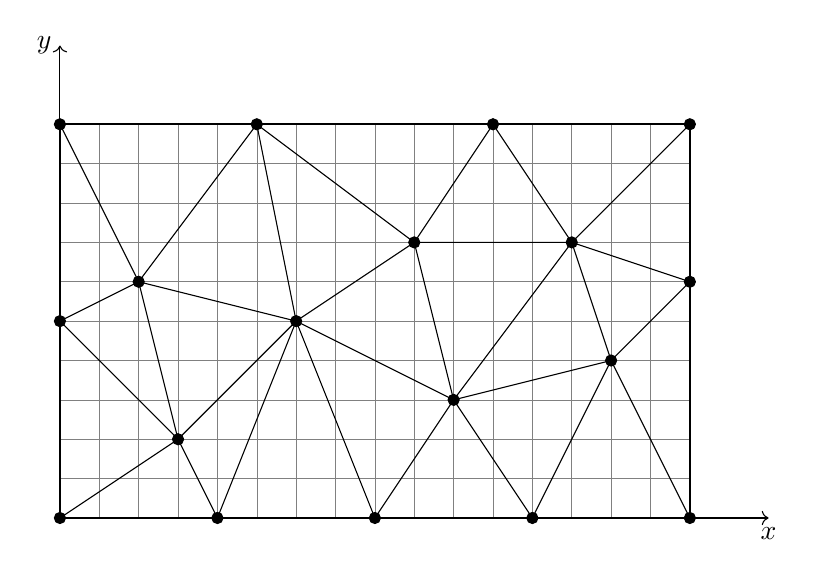
\begin{tikzpicture}
%\draw[fill=gray!8,gray!8](0,0) rectangle (10,7);
\draw[step=0.5cm,gray,very thin] (1,1) grid (9,6); %background grid
\draw[thick] (1,1) -- (9,1) -- (9,6) -- (1,6) -- cycle;  

\draw[thin,->] (1,1) -- (10,1) ; %horizontal axis
\draw[thin,->] (1,1) -- (1,7) ; %horizontal axis
\node[] at (10,0.8){$x$};
\node[] at (0.8,7){$y$};

\draw[] (1,1) -- (2.5,2) -- (4,3.5) -- (5.5,4.5) -- (6.5,6);  %1 6 11 13 14
\draw[] (3,1) -- (4,3.5) -- (6,2.5) -- (7.5,4.5) -- (9,6) ;  %2 11 12 15 16
\draw[] (3,1) -- (2.5,2) -- (1,3.5) -- (2,4) -- (1,6) ;  %2 6 7 8 9
\draw[] (5,1) -- (6,2.5) -- (7,1) -- (8,3) -- (9,4) -- (7.5,4.5) -- (6.5,6) ;  %3 12 4 18 17 15 14
\draw[] (3.5,6) -- (2,4) -- (4,3.5) -- (5,1) ;  %10 8 11 3
\draw[] (2.5,2) -- (2,4) ; %6 8
\draw[] (4,3.5) -- (3.5,6) -- (5.5,4.5) -- (7.5,4.5) ;  %11 10 13 15
\draw[] (9,1) -- (8,3) -- (6,2.5) -- (5.5,4.5) ;  %5 18 12 13
\draw[] (7.5,4.5) -- (8,3) ; %15 18

\draw[black,fill=black] (1,1)     circle (2pt); 
\draw[black,fill=black] (3,1)     circle (2pt); 
\draw[black,fill=black] (5,1)     circle (2pt); 
\draw[black,fill=black] (7,1)     circle (2pt); 
\draw[black,fill=black] (9,1)     circle (2pt); 
\draw[black,fill=black] (2.5,2)   circle (2pt); 
\draw[black,fill=black] (1,3.5)   circle (2pt); 
\draw[black,fill=black] (2,4)     circle (2pt); 
\draw[black,fill=black] (1,6)     circle (2pt); 
\draw[black,fill=black] (3.5,6)   circle (2pt); 
\draw[black,fill=black] (4,3.5)   circle (2pt); 
\draw[black,fill=black] (6,2.5)   circle (2pt); 
\draw[black,fill=black] (5.5,4.5) circle (2pt); 
\draw[black,fill=black] (6.5,6)   circle (2pt); 
\draw[black,fill=black] (7.5,4.5) circle (2pt); 
\draw[black,fill=black] (9,6)     circle (2pt); 
\draw[black,fill=black] (9,4)     circle (2pt); 
\draw[black,fill=black] (8,3)     circle (2pt); 

\end{tikzpicture}\\
\end{center}
         
We can first label the nodes:

\begin{center}
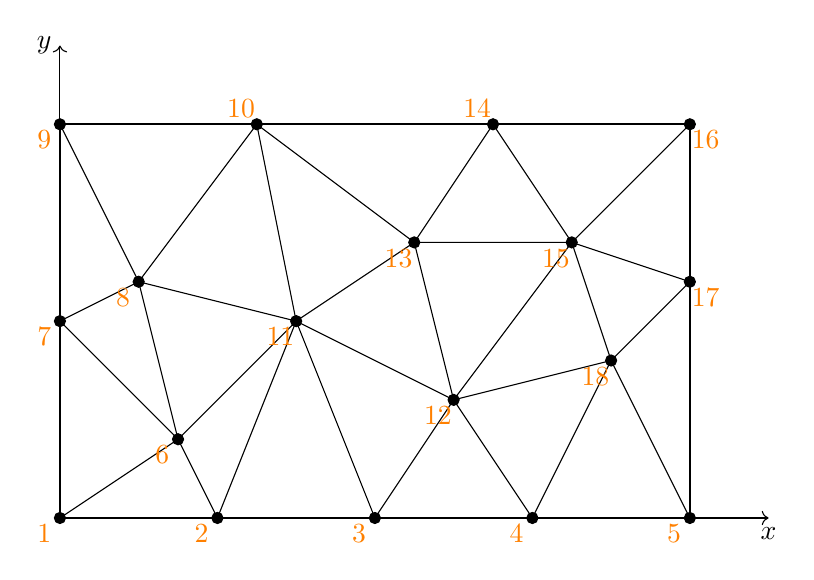
\begin{tikzpicture}
%\draw[fill=gray!5,gray!5](0,0) rectangle (10,7);
%\draw[step=0.5cm,gray,very thin] (1,1) grid (9,6); %background grid
\draw[thick] (1,1) -- (9,1) -- (9,6) -- (1,6) -- cycle;  

\draw[thin,->] (1,1) -- (10,1) ; %horizontal axis
\draw[thin,->] (1,1) -- (1,7) ; %horizontal axis
\node[] at (10,0.8){$x$};
\node[] at (0.8,7){$y$};


\draw[] (1,1) -- (2.5,2) -- (4,3.5) -- (5.5,4.5) -- (6.5,6);  %1 6 11 13 14
\draw[] (3,1) -- (4,3.5) -- (6,2.5) -- (7.5,4.5) -- (9,6) ;  %2 11 12 15 16
\draw[] (3,1) -- (2.5,2) -- (1,3.5) -- (2,4) -- (1,6) ;  %2 6 7 8 9
\draw[] (5,1) -- (6,2.5) -- (7,1) -- (8,3) -- (9,4) -- (7.5,4.5) -- (6.5,6) ;  %3 12 4 18 17 15 14
\draw[] (3.5,6) -- (2,4) -- (4,3.5) -- (5,1) ;  %10 8 11 3
\draw[] (2.5,2) -- (2,4) ; %6 8
\draw[] (4,3.5) -- (3.5,6) -- (5.5,4.5) -- (7.5,4.5) ;  %11 10 13 15
\draw[] (9,1) -- (8,3) -- (6,2.5) -- (5.5,4.5) ;  %5 18 12 13
\draw[] (7.5,4.5) -- (8,3) ; %15 18

\draw[black,fill=black] (1,1)     circle (2pt); \node[] at (0.8,0.8){\color{orange} 1}; %1
\draw[black,fill=black] (3,1)     circle (2pt); \node[] at (2.8,0.8){\color{orange} 2}; %2
\draw[black,fill=black] (5,1)     circle (2pt); \node[] at (4.8,0.8){\color{orange} 3}; %3
\draw[black,fill=black] (7,1)     circle (2pt); \node[] at (6.8,0.8){\color{orange} 4}; %4
\draw[black,fill=black] (9,1)     circle (2pt); \node[] at (8.8,0.8){\color{orange} 5}; %5
\draw[black,fill=black] (2.5,2)   circle (2pt); \node[] at (2.3,1.8){\color{orange} 6}; %6
\draw[black,fill=black] (1,3.5)   circle (2pt); \node[] at (0.8,3.3){\color{orange} 7}; %7
\draw[black,fill=black] (2,4)     circle (2pt); \node[] at (1.8,3.8){\color{orange} 8}; %8
\draw[black,fill=black] (1,6)     circle (2pt); \node[] at (0.8,5.8){\color{orange} 9}; %9
\draw[black,fill=black] (3.5,6)   circle (2pt); \node[] at (3.3,6.2){\color{orange} 10};%10
\draw[black,fill=black] (4,3.5)   circle (2pt); \node[] at (3.8,3.3){\color{orange} 11};%11
\draw[black,fill=black] (6,2.5)   circle (2pt); \node[] at (5.8,2.3){\color{orange} 12};%12
\draw[black,fill=black] (5.5,4.5) circle (2pt); \node[] at (5.3,4.3){\color{orange} 13};%13
\draw[black,fill=black] (6.5,6)   circle (2pt); \node[] at (6.3,6.2){\color{orange} 14};%14
\draw[black,fill=black] (7.5,4.5) circle (2pt); \node[] at (7.3,4.3){\color{orange} 15};%15
\draw[black,fill=black] (9,6)     circle (2pt); \node[] at (9.2,5.8){\color{orange} 16};%16
\draw[black,fill=black] (9,4)     circle (2pt); \node[] at (9.2,3.8){\color{orange} 17};%17
\draw[black,fill=black] (8,3)     circle (2pt); \node[] at (7.8,2.8){\color{orange} 18};%18
\end{tikzpicture}\\
\end{center}

and then label the elements:

\begin{center}
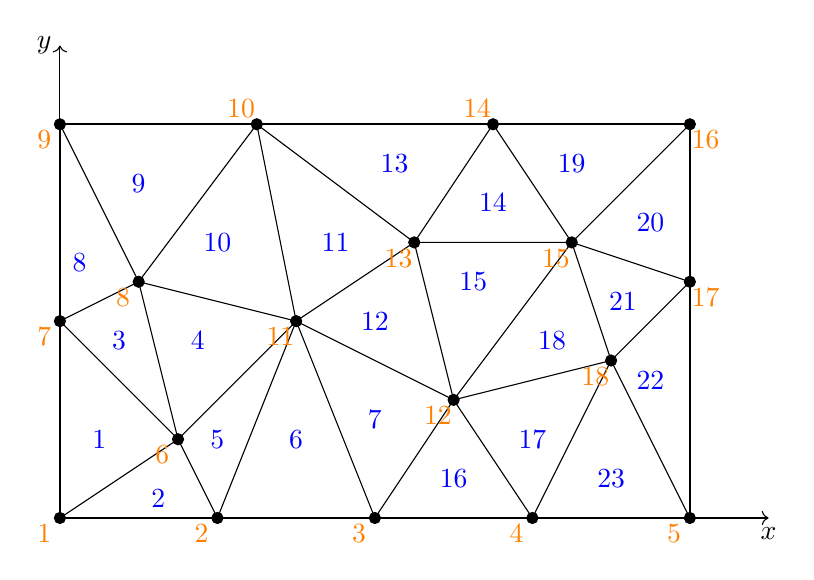
\begin{tikzpicture}
%\draw[fill=gray!5,gray!5](0,0) rectangle (10,7);
%\draw[step=0.5cm,gray,very thin] (1,1) grid (9,6); %background grid
\draw[thick] (1,1) -- (9,1) -- (9,6) -- (1,6) -- cycle;  

\draw[thin,->] (1,1) -- (10,1) ; %horizontal axis
\draw[thin,->] (1,1) -- (1,7) ; %horizontal axis
\node[] at (10,0.8){$x$};
\node[] at (0.8,7){$y$};


\draw[] (1,1) -- (2.5,2) -- (4,3.5) -- (5.5,4.5) -- (6.5,6);  %1 6 11 13 14
\draw[] (3,1) -- (4,3.5) -- (6,2.5) -- (7.5,4.5) -- (9,6) ;  %2 11 12 15 16
\draw[] (3,1) -- (2.5,2) -- (1,3.5) -- (2,4) -- (1,6) ;  %2 6 7 8 9
\draw[] (5,1) -- (6,2.5) -- (7,1) -- (8,3) -- (9,4) -- (7.5,4.5) -- (6.5,6) ;  %3 12 4 18 17 15 14
\draw[] (3.5,6) -- (2,4) -- (4,3.5) -- (5,1) ;  %10 8 11 3
\draw[] (2.5,2) -- (2,4) ; %6 8
\draw[] (4,3.5) -- (3.5,6) -- (5.5,4.5) -- (7.5,4.5) ;  %11 10 13 15
\draw[] (9,1) -- (8,3) -- (6,2.5) -- (5.5,4.5) ;  %5 18 12 13
\draw[] (7.5,4.5) -- (8,3) ; %15 18

\draw[black,fill=black] (1,1)     circle (2pt); \node[] at (0.8,0.8){\color{orange} 1}; %1
\draw[black,fill=black] (3,1)     circle (2pt); \node[] at (2.8,0.8){\color{orange} 2}; %2
\draw[black,fill=black] (5,1)     circle (2pt); \node[] at (4.8,0.8){\color{orange} 3}; %3
\draw[black,fill=black] (7,1)     circle (2pt); \node[] at (6.8,0.8){\color{orange} 4}; %4
\draw[black,fill=black] (9,1)     circle (2pt); \node[] at (8.8,0.8){\color{orange} 5}; %5
\draw[black,fill=black] (2.5,2)   circle (2pt); \node[] at (2.3,1.8){\color{orange} 6}; %6
\draw[black,fill=black] (1,3.5)   circle (2pt); \node[] at (0.8,3.3){\color{orange} 7}; %7
\draw[black,fill=black] (2,4)     circle (2pt); \node[] at (1.8,3.8){\color{orange} 8}; %8
\draw[black,fill=black] (1,6)     circle (2pt); \node[] at (0.8,5.8){\color{orange} 9}; %9
\draw[black,fill=black] (3.5,6)   circle (2pt); \node[] at (3.3,6.2){\color{orange} 10};%10
\draw[black,fill=black] (4,3.5)   circle (2pt); \node[] at (3.8,3.3){\color{orange} 11};%11
\draw[black,fill=black] (6,2.5)   circle (2pt); \node[] at (5.8,2.3){\color{orange} 12};%12
\draw[black,fill=black] (5.5,4.5) circle (2pt); \node[] at (5.3,4.3){\color{orange} 13};%13
\draw[black,fill=black] (6.5,6)   circle (2pt); \node[] at (6.3,6.2){\color{orange} 14};%14
\draw[black,fill=black] (7.5,4.5) circle (2pt); \node[] at (7.3,4.3){\color{orange} 15};%15
\draw[black,fill=black] (9,6)     circle (2pt); \node[] at (9.2,5.8){\color{orange} 16};%16
\draw[black,fill=black] (9,4)     circle (2pt); \node[] at (9.2,3.8){\color{orange} 17};%17
\draw[black,fill=black] (8,3)     circle (2pt); \node[] at (7.8,2.8){\color{orange} 18};%18


\node[] at (1.5,2) {\color{blue}1};
\node[] at (2.25,1.25) {\color{blue}2};
\node[] at (1.75,3.25) {\color{blue}3};
\node[] at (2.75,3.25) {\color{blue}4};
\node[] at (3,2) {\color{blue}5};
\node[] at (4,2) {\color{blue}6};
\node[] at (5,2.25) {\color{blue}7};
\node[] at (1.25,4.25) {\color{blue}8};
\node[] at (2,5.25) {\color{blue}9};
\node[] at (3,4.5) {\color{blue}10};
\node[] at (4.5,4.5) {\color{blue}11};
\node[] at (5,3.5) {\color{blue}12};
\node[] at (5.25,5.5) {\color{blue}13};
\node[] at (6.5,5) {\color{blue}14};
\node[] at (6.25,4) {\color{blue}15};
\node[] at (6,1.5) {\color{blue}16};
\node[] at (7,2) {\color{blue}17};
\node[] at (7.25,3.25) {\color{blue}18};
\node[] at (7.5,5.5) {\color{blue}19};
\node[] at (8.5,4.75) {\color{blue}20};
\node[] at (8.15,3.75) {\color{blue}21};
\node[] at (8.5,2.75) {\color{blue}22};
\node[] at (8,1.5) {\color{blue}23};


\end{tikzpicture}\\
\end{center}

We can finally build the connectivity array by hand:

\noindent
icon(1,{\color{blue}1})={\color{orange}1}\\
icon(2,{\color{blue}1})={\color{orange}6}\\
icon(3,{\color{blue}1})={\color{orange}7}\\
icon(1,{\color{blue}2})={\color{orange}1}\\
icon(2,{\color{blue}2})={\color{orange}2}\\
icon(3,{\color{blue}2})={\color{orange}6}\\
icon(1,{\color{blue}3})={\color{orange}7}\\
icon(2,{\color{blue}3})={\color{orange}6}\\
icon(3,{\color{blue}3})={\color{orange}8}\\
...\\
icon(1,{\color{blue}12})={\color{orange}11}\\
icon(2,{\color{blue}12})={\color{orange}12}\\
icon(3,{\color{blue}12})={\color{orange}13}\\
...\\
icon(1,{\color{blue}19})={\color{orange}14}\\
icon(2,{\color{blue}19})={\color{orange}15}\\
icon(3,{\color{blue}19})={\color{orange}16}\\


The labelling of nodes and elements above is done by a human so it starts at 1. When 
implementing this in python, you know what to do ...


%-----------------------------------------------
\section{How to visualise data on a triangular mesh with Paraview}

If arrays {\tt x,y} contain the coordinates of the nodes, your connectivity array is called {\tt icon},
and your mesh consistes of {\tt nel} elements and comprises {\tt nnp} nodes, you can use the following code
to generate a vtu file to be opened with Paraview. You also need a temperature array {\tt T}.

\begin{center}
Code at \url{https://raw.githubusercontent.com/cedrict/fieldstone/master/images/compgeo/mesh_visu.py}
\end{center}

\lstinputlisting[language=python]{images/compgeo/mesh_visu.py}


%==============================================================================
\section{Writing a report as homework \label{app:grading}} 

\begin{itemize}
\item 
The document should contain your full name and student number on the first page. 
\item 
The file should be a pdf which name contains your family name
\item 
Layout: is the document visually pleasing? Is it well structured? 
\item Is there a complete bibliography (when applicable)?
\item Does the structure follows this: Introduction - Methods - Results - Discussion - Conclusion - Appendix ?
\item 
Figures: Are they properly numbered? captioned? all figures must be referenced in the text. 
Are they of good enough quality (no visible pixels)? are they readable? are all axis labelled?
\item 
Text: Overall quality of the language. Are there still typos? Do all sentence make sense?
\item if you wish to show lines of code, use verbatim or lstlisting\footnote{\url{https://en.wikibooks.org/wiki/LaTeX/Source_Code_Listings}} 
\item 
Discussion: are the results properly discussed, analyzed? are potential problems, errors, limitations discussed?
\item 
Conclusion: Are the findings/results summarized and generalized?
\end{itemize}

\begin{center}
\begin{tabular}{cc}
\hline
No & Yes \\
\hline
\hline
$6.67*10^{-11}$ & $6.67 \times 10^{-11}$ \\
$kg/m^3$ &  kg/m$^{3}$ or kg.m$^{-3}$\\
1x1 & 1$\times$1\\
$cos$ & $\cos$\\
docx file & pdf file \\
'if you do this'& passive form \\ 
\hline
\end{tabular}
\end{center}




%.....................................
\par\noindent\rule{\textwidth}{0.4pt}
\begin{center}
\includegraphics[width=10cm]{images/grading/grey}\\
No grey background
\end{center}


%.....................................
\par\noindent\rule{\textwidth}{0.4pt}
\begin{center}
\includegraphics[width=10cm]{images/grading/numbers}\\
No lists/arrays with numbers
\end{center}

%.....................................
\par\noindent\rule{\textwidth}{0.4pt}
\begin{center}
\includegraphics[width=10cm]{images/grading/arrows2}\\
Too many arrows\\
\includegraphics[width=9cm]{images/grading/arrows1}\\
Poor choice of arrow colour
\end{center}

%.....................................
\par\noindent\rule{\textwidth}{0.4pt}
\begin{center}
\includegraphics[width=8cm]{images/grading/pixels1}
\includegraphics[width=7cm]{images/grading/pixels2}\\
Be careful about how you export your figures. These are unreadable.
\end{center}
 
%.....................................
\par\noindent\rule{\textwidth}{0.4pt}
\begin{center}
\includegraphics[width=8cm]{images/grading/eqs1}\\
Parenthesis too small
\end{center}

%.....................................
\par\noindent\rule{\textwidth}{0.4pt}
\begin{center}
\includegraphics[width=9cm]{images/grading/eqs2}\\
1.6E+10 is not acceptable. Replace by $1.6\cdot 10^{10}$
\end{center}

%.....................................
\par\noindent\rule{\textwidth}{0.4pt}
\begin{center}
\includegraphics[width=7cm]{images/grading/eqs3}\\
Equation number is too close to the equation itself. Use labels, 
do not number equations by hand.
\end{center}

%.....................................
\par\noindent\rule{\textwidth}{0.4pt}
\begin{center}
\includegraphics[width=9cm]{images/grading/eqs4}\\
Formatting of both axis lead to unreadable figure.
\end{center}

%.....................................
\par\noindent\rule{\textwidth}{0.4pt}
\begin{center}
\includegraphics[width=9cm]{images/grading/eqs5}\\
In \LaTeX{}  use \verb!\sum\limits!
\end{center}

%.....................................
\par\noindent\rule{\textwidth}{0.4pt}
\begin{center}
\includegraphics[width=9cm]{images/grading/eqs6}\\
Are so many digits necessary?
\end{center}

%.....................................
\par\noindent\rule{\textwidth}{0.4pt}
\begin{center}
\includegraphics[width=12cm]{images/grading/width}\\
use \verb!\usepackage[cm]{fullpage}! to allow for wider text.
\end{center}

%.....................................
\par\noindent\rule{\textwidth}{0.4pt}
\begin{center}
\includegraphics[width=10cm]{images/grading/figs1}\\
This figure style is to be avoided. Simply use dots and/or lines.
\end{center}

%.....................................
\par\noindent\rule{\textwidth}{0.4pt}
\begin{center}
\includegraphics[width=8cm]{images/grading/figs2}
\end{center}

%.....................................
\par\noindent\rule{\textwidth}{0.4pt}
\begin{center}
\includegraphics[width=6cm]{images/grading/loglogpb}\\
Here Ra and Nu are plotted in log-log scale, not log(Ra) and log(Nu).
\end{center}

%.....................................
\par\noindent\rule{\textwidth}{0.4pt}
\begin{center}
\includegraphics[width=10cm]{images/grading/dots}\\
The dots at the beginning and end of the lines are not necessary.
\end{center}

%.....................................
\par\noindent\rule{\textwidth}{0.4pt}
\begin{center}
\includegraphics[width=11cm]{images/grading/you}\\
Never {\it never} use 'you'. 
\end{center}

%.....................................
\par\noindent\rule{\textwidth}{0.4pt}
\begin{center}
\includegraphics[width=10cm]{images/grading/cross}\\
Do not use 'X' but $\times$ (\verb|\times|).
\end{center}




\begin{itemize}
\item The report should be in \LaTeX 
\item The document should contain your full name and student number on the first page. 
\item The report file should be a pdf which name contains your family name
\item not more than 25 pages. If more, use appendices wisely.
\item document should be structured in two main parts: FDM and FEM.
\item no equations unless necessary to the discussion (still mention the equation that 
you are solving but refer to an external document/article/book for example).
\item use lstlisting package to include code
\item use {\verb| \usepackage[cm]{fullpage} |} to format your document
\item all codes either in appendix or in zip file (bearing your name).
\item a decent introduction (half page to one page) which links the topic of this course to geosciences.
\item discussion of results (stability, convergence, influence of resolution, remarks of all kinds).
\item if you did not succeed in doing a particular exercise, please explain what you think the problem is, 
how you know it is not working, etc ...
\item think about colormaps, image compression
%\item DEADLINE: July 16th, 2023, 23:59 
\end{itemize}


I will use this table to grade your reports:

\vspace{2cm}


\begin{tabular}{|p{5cm}|p{.35cm}|p{.35cm}|p{.35cm}|p{.35cm}|p{.35cm}|p{.35cm}|p{.35cm}|p{.35cm}|p{.35cm}|p{.35cm}|p{.35cm}|p{.35cm}|p{.35cm}|p{.35cm}|p{.35cm}|}
&&&&&&&&&&&&&&& \\
\hline
title, names, student nb &&&&&&&&&&&&&&& \\\hline
\LaTeX ? &&&&&&&&&&&&&&& \\\hline
document layout &&&&&&&&&&&&&&& \\\hline
equations look &&&&&&&&&&&&&&& \\\hline
equations numbered  &&&&&&&&&&&&&&& \\\hline
use of equations &&&&&&&&&&&&&&& \\\hline
figs: caption &&&&&&&&&&&&&&& \\\hline
figs: pixels? &&&&&&&&&&&&&&& \\\hline
figs: correct? &&&&&&&&&&&&&&& \\\hline
English grammar &&&&&&&&&&&&&&& \\\hline
Typos 
Introduction &&&&&&&&&&&&&&& \\\hline
methods/results &&&&&&&&&&&&&&& \\\hline
Discussion/Conclusion  &&&&&&&&&&&&&&& \\\hline
Extra work? &&&&&&&&&&&&&&& \\\hline
Bibliography &&&&&&&&&&&&&&& \\\hline
code layout &&&&&&&&&&&&&&& \\\hline 
code style &&&&&&&&&&&&&&& \\\hline
code accuracy &&&&&&&&&&&&&&& \\\hline
\end{tabular}





 %%%%%%%%%%%%%%%%%%%%%%%%%%%
\chapter{Using prisms in forward gravity modelling \label{app:prisms}} \input{app_prisms} %%%%%%%%%
\chapter{Solutions to exercises of GEO3-1313 \label{app:gravsols}} 
%------------------------------
\subsection{Problem 1}

\begin{center}
\includegraphics[width=4cm]{images/sphcoord}
\end{center}

\begin{eqnarray}
I 
&=& \frac{1}{3} (I_x + I_y + I_z ) \nn\\
&=& 
\frac{1}{3} \iiint_V \rho(r) (y^2+z^2) dV +
\frac{1}{3} \iiint_V \rho(r) (x^2+z^2) dV +
\frac{1}{3} \iiint_V \rho(r) (x^2+y^2) dV \nn\\
&=&
\frac{1}{3} \iiint_V \rho(r) (2x^2 + 2y^2+2z^2) dV \nn\\
&=&
\frac{2}{3} \iiint_V \rho(r) r^2 dV \nn\\
&=& \frac{2}{3} \iiint_V \rho(r) r^2 r^2 \sin\theta dr \; d\theta \; d\phi \nn\\
&=& \frac{2}{3} \int_0^R \int_0^\pi \int_0^{2\pi}    \rho(r) r^2 r^2 \sin\theta dr \; d\theta \; d\phi \nn\\
&=& \frac{2}{3} \left(\int_0^\pi \sin\theta d\theta \right)
\left( \int_0^{2\pi} d\phi \right)  \int_0^R   \rho(r) r^4 dr \nn\\
&=& \frac{8\pi}{3}  \int_0^R   \rho(r) r^4 dr 
\end{eqnarray}

Alternative solution:
$I$ is evaluated for the special case where the rotation axis is the $z$-axis, 
where $d = r sin\theta$. 
Substitution in $I=\int_V \rho d^2 dV$ yields
\begin{eqnarray}
I
&=& \iiint_V \rho(r) (r^2 \sin^2\theta ) dV  \nn\\
&=& \int_0^R \int_0^\pi \int_0^{2\pi} \rho(r) ( r^2 \sin^2\theta ) r^2 \sin\theta dr \; d\theta \; d\phi \nn\\
&=& \left(\int_0^\pi \sin^3 \theta d\theta \right)
\left( \int_0^{2\pi} d\phi \right)  \int_0^R   \rho(r) r^4 dr \nn
\end{eqnarray}
By writing $\sin^3\theta = \sin\theta (1-\cos^2\theta)$ we can operate a change of variables $u=\cos \theta$,
and we arrive at $\int \sin^3 \theta d\theta=4/3$ (skipping a few steps here) 
and we obtain the expected result.






\newpage
%------------------------------
\subsection{Problem 2}

For a uniform sphere, we have $\rho(r)=\rho_0$. Then 

\begin{eqnarray}
I 
&=& \frac{8\pi}{3}  \int_0^R   \rho_0 r^4 dr \nn\\
&=& \frac{8\pi}{3}\rho_0  \int_0^R  r^4 dr \nn\\
&=& \frac{8\pi}{15}\rho_0 R^5  \int_0^R  r^4 dr \nn
\end{eqnarray}

The mass of the sphere is
\begin{eqnarray}
M 
&=& \iiint_V \rho(r) dV \nn\\
&=& \rho_0 \int_0^R \int_0^\pi \int_0^{2\pi}   r^2 \sin\theta dr \; d\theta \; d\phi \nn\\
&=& \rho_0 \frac{4}{3} \pi R^3
\end{eqnarray}

In the end we get
\[
I = \frac{2}{5} M R^2
\]


When all the mass is concentrated in the center, then $\rho(r)= \rho_0 \delta(r)$ where 
$\delta$ is the Dirac delta function\footnote{\url{https://en.wikipedia.org/wiki/Dirac_delta_function}}.
Then 
\begin{eqnarray}
I 
&=& \frac{8\pi}{3}  \int_0^R   \rho_0 \delta(r) r^4 dr \nn\\
&=& \frac{8\pi}{3} \rho_0  \int_0^R  \delta(r) r^4 dr \nn\\
&=& 0
\end{eqnarray}

When all the mass is concentrated in a shell of zero thickness of radius $R$, 
then $\rho(r)= \rho_0 \delta(r-R)$, so 
\begin{eqnarray}
I 
&=& \frac{8\pi}{3}  \int_0^R   \rho_0 \delta(r-R) r^4 dr \nn\\
&=& \frac{8\pi}{3} \rho_0  \int_0^R  \delta(r-R) r^4 dr \nn\\
&=& \frac{8\pi}{3} \rho_0  R^4
\end{eqnarray}
Conversely, its mass is 
\begin{eqnarray}
M 
&=& \iiint_V \rho(r) dV \nn\\
&=& \rho_0 \int_0^R \int_0^\pi \int_0^{2\pi} \delta(r-R)  r^2 \sin\theta dr \; d\theta \; d\phi \nn\\
&=& \rho_0 4  \pi R^2
\end{eqnarray}
and then 
\[
I = \frac{2}{3} M R^2
\]



\newpage
%------------------------------
\subsection{Problem 3}


\begin{eqnarray}
\langle \rho \rangle 
&=& \frac{1}{V} \iiint_V \rho dV \nn\\
&=& \frac{1}{\frac{4}{3}\pi R^3} \iiint_V \rho(r) r^2 \sin\theta dr \; d\theta d\phi \nn\\
&=& \frac{1}{\frac{4}{3}\pi R^3}  4\pi \int_0^R \rho(r) r^2  dr \nn\\
&=& \frac{3}{R^3}   \int_0^R \rho(r) r^2  dr  \label{appgravsols3}
\end{eqnarray}

We then turn to the moment of inertia:
\begin{eqnarray}
I 
&=& \frac{8\pi}{3} \int_0^R \rho(r) r^4 dr \label{appgravsols2}\\
&=& f M R^2 \label{appgravsols1}
\end{eqnarray}
where 
\[
M 
= \iiint_V \rho(r) dV 
= V \; \underbrace{\frac{1}{V} \iiint_V \rho(r) dV }_{\langle\rho\rangle}
= \frac{4}{3}\pi R^3 \langle\rho\rangle
\]
We then insert this expression of $M$ in Eq.~\eqref{appgravsols1}:
\[
I
= f \frac{4}{3}\pi R^3 \langle\rho\rangle R^2
= f \frac{4}{3}\pi R^5 \langle\rho\rangle 
\]
Equating this to Eq.~\ref{appgravsols2} yields
\[
\frac{8\pi}{3} \int_0^R \rho(r) r^4 dr = f \frac{4}{3}\pi R^5 \langle\rho\rangle
\]
or, 
\begin{equation}
f \langle \rho \rangle R^5 = 2 \int_0^R \rho(r) r^4 dr  \label{appgravsols4}
\end{equation}


We now make use of the expression for the density:
\[
\rho(r) =
\left\{
\begin{array}{ll}
\rho_c & 0\leq r \leq R_c \\
\rho_m & R_c\leq r \leq R 
\end{array}
\right.
\]
Then Eq.~\eqref{appgravsols3} yields
\begin{eqnarray}
\langle \rho \rangle 
&=& \frac{3}{R^3}   \int_0^R \rho(r) r^2  dr \nn\\
&=& \frac{3}{R^3} \left(   \int_0^{R_c} \rho_c r^2  dr +  \int_{R_c}^R \rho_m r^2  dr \right) \nn\\
&=& \frac{3}{R^3} \left(  \frac{R_c^3}{3} \rho_c  +   \frac{1}{3}(R^3-R_c^3) \rho_m \right) \nn\\
&=&   \frac{R_c^3}{R^3} \rho_c  +   (1-\frac{R_c^3}{R^3}) \rho_m  \nn\\
&=&   \left(\frac{R_c}{R}\right)^3 \rho_c  +   \left[1-\left(\frac{R_c}{R}\right)^3\right] \rho_m 
\end{eqnarray}
We know $\rho_m$, but not $\rho_c$, so we write:
\begin{equation}
\rho_c 
=\rho_m \left[ 1 + \left(\frac{R}{R_c}\right)^3 \left(\frac{\langle \rho \rangle}{\rho_m} -1\right) \right]
\label{appgravsols5} 
\end{equation}

We now turn to Eq.~\eqref{appgravsols4}. Since 
\begin{eqnarray}
2 \int_0^R \rho(r) r^4 dr 
&=&   2 \int_0^{R_c} \rho_c r^4 dr +  2 \int_{R_c}^R \rho_m r^4 dr \nn\\
&=& \frac{2}{5} \left[ R_c^5  \rho_c + (R^5-R_c^5) \rho_m  \right]  \nn
\end{eqnarray}
then 
\[
f \langle \rho \rangle R^5 = \frac{2}{5} \left[ R_c^5  \rho_c + (R^5-R_c^5) \rho_m  \right] 
\]
or, 
\[
\frac{5 f \langle \rho \rangle R^5}{2 \rho_m} =   R_c^5  \frac{\rho_c}{\rho_m} + (R^5-R_c^5)  
\]
\[
\frac{5 f \langle \rho \rangle R^5}{2 \rho_m} =   R_c^5  (\frac{\rho_c}{\rho_m}-1) + R^5)  
\]
Now dividing by $R^5$ on each side:
\[
\frac{5 f \langle \rho \rangle }{2 \rho_m} =  \left(\frac{R_c}{R}\right)^5    \left(\frac{\rho_c}{\rho_m}-1 \right) + 1 
\]
Using Eq.~\eqref{appgravsols5}, we can write 
\[
\frac{\rho_c}{\rho_m}-1  = 
\left(\frac{R}{R_c}\right)^3 \left(\frac{\langle \rho \rangle}{\rho_m} -1\right) 
\]
so finally
\[
\frac{5 f \langle \rho \rangle }{2 \rho_m} - 1=  \left(\frac{R_c}{R}\right)^5     
\left(\frac{R}{R_c}\right)^3 \left(\frac{\langle \rho \rangle}{\rho_m} -1\right) 
\]
or, 
\[
\frac{5 f \langle \rho \rangle }{2 \rho_m} - 1=  \left(\frac{R_c}{R}\right)^2     
 \left(\frac{\langle \rho \rangle}{\rho_m} -1\right) 
\]
and then 
\[
\left(\frac{R_c}{R}\right)
=
\left( 
\frac{ \frac{5 f \langle \rho \rangle }{2 \rho_m} - 1  }{  \left(\frac{\langle \rho \rangle}{\rho_m} -1\right)  }
\right)^{1/2}
\]




\newpage
%------------------------------
\subsection{Problem 4}

Assume a uniform mantle $\rho_m$ and core $\rho_c$. For the total mass we have 
\[
M=\int_V \rho dV = 4\pi \int_0^R \rho(r) r^2 dr 
=
\frac{4\pi}{3} R_c^3 \rho_c + \frac{4\pi}{3} (R^3-R_c^3) \rho_m
\]
For the moment of inertia we have,
\[
I 
= \frac{8\pi}{3} \int_0^R \rho(r) r^4 dr
= 
\frac{8\pi}{15} R_c^5 \rho_c + \frac{8\pi}{15} (R^5-R_c^5) \rho_m
\]
In matrix form the above equations become:
\[
\left(
\begin{array}{cc}
\frac{4\pi}{3} R_c^3  & \frac{4\pi}{3} (R^3-R_c^3) \\
\frac{8\pi}{15} R_c^5 &  \frac{8\pi}{15} (R^5-R_c^5) 
\end{array}
\right)
\cdot
\left(
\begin{array}{cc}
\rho_c \\ \rho_m
\end{array}
\right)
=
\left(
\begin{array}{cc}
M & I
\end{array}
\right)
\]
We use Cramers rule
\[
\left(
\begin{array}{cc}
a11 & a12 \\
a21 & a22
\end{array}
\right)
\cdot
\left(
\begin{array}{c}
x_1 \\ x_2
\end{array}
\right)
=
\left(
\begin{array}{c}
b_1 \\ b_2
\end{array}
\right)
\qquad
\Rightarrow
\qquad
\left(
\begin{array}{c}
x_1 \\ x_2
\end{array}
\right)
=
\frac{1}{\Delta}
\left(
\begin{array}{cc}
a22 & -a12 \\
-a21 & a11
\end{array}
\right)
\cdot
\left(
\begin{array}{c}
b_1 \\ b_2
\end{array}
\right)
\]
In our case the determinant of the matrix is 
\[
\Delta = \frac{32\pi^2}{45}\left[ R_c^3(R^5-R_c^3)-R_c^5(R^3-R_c^3)   \right]
\]



%------------------------------
\subsection{Problem 5}

skipped 

%------------------------------
\subsection{Problem 6}

see lecture notes


%------------------------------
\subsection{Problem 7}

\[
g = \frac{{\cal G}M}{R^2} = \frac{6.67e-11*5.97e24}{6371000^2} \simeq 9.8
\]

%------------------------------
\subsection{Problem 8}

\[
p_{CMB} = \int \rho g dz \simeq \rho_0 g_0 (R_{Earth}-R_{CMB}) \simeq 127.5GPa
\]


\newpage
%------------------------------
\subsection{Problem 9}

\[
U(\vec{r}) 
= -\frac{{\cal G} m_1}{|\vec{r}_1 - \vec{r}|} 
= -\frac{{\cal G} m_1}{\sqrt{(x_1-x)^2+(y_1-y)^2+(z_1-z)^2}} 
\]

\[
\vec\nabla U = 
\left(
\begin{array}{c}
\partial_x U \\
\partial_y U \\
\partial_z U 
\end{array}
\right)
\]

We have 
\begin{eqnarray}
\partial_x U 
&=&  -{\cal G} m_1 \frac{\partial }{\partial x} \frac{1}{\sqrt{(x_1-x)^2+(y_1-y)^2+(z_1-z)^2}} \nn\\
&=&  -{\cal G} m_1 \cdot -\frac{1}{2}  \frac{-2(x_1-x)}{[(x_1-x)^2+(y_1-y)^2+(z_1-z)^2]^{3/2}} \nn\\
&=&  {\cal G} m_1  \frac{1}{[(x_1-x)^2+(y_1-y)^2+(z_1-z)^2]} \frac{-(x_1-x)}{\sqrt{(x_1-x)^2+(y_1-y)^2+(z_1-z)^2}} \nn\\
&=&  {\cal G} m_1  \frac{1}{|\vec{r}_1 - \vec{r}|^2} \frac{-(x_1-x)}{\sqrt{(x_1-x)^2+(y_1-y)^2+(z_1-z)^2}} \nn
\end{eqnarray}
We repeat this operation for $\partial_y$ and $\partial_z$ and finally:

\[
-\vec\nabla U = 
\left(
\begin{array}{c}
\partial_x U \\
\partial_y U \\
\partial_z U 
\end{array}
\right)
=  {\cal G} m_1  \frac{1}{|\vec{r}_1 - \vec{r}|^2} 
\left(
\begin{array}{c}
\frac{(x_1-x)}{|\vec{r}_1 - \vec{r}|} \\
\frac{(y_1-y)}{|\vec{r}_1 - \vec{r}|} \\
\frac{(z_1-z)}{|\vec{r}_1 - \vec{r}|} \\
\end{array}
\right)
=
\frac{ {\cal G} m_1}{|\vec{r}_1 - \vec{r}|^2} \vec{e}_{\vec{r}_1\vec{r}} = \vec{g}
\]


%------------------------------
\subsection{Problem 10}

\[
\int_V \Delta U dV
=
\int_V 4\pi {\cal G} \rho dV
=
4\pi {\cal G} \int_V M \delta(\vec{r}-\vec{r}_0) dV
=
4 \pi {\cal G} M
\] 


\[
\int_V \Delta U dV 
=
\int_V \vec\nabla^2 U dV
=
\int_V \vec\nabla \cdot \vec\nabla U dV
=
\int_\Gamma \vec\nabla U \cdot \vec n dS
=
\int_\Gamma ( - \vec{g}) \cdot \vec n dS
=
\int_\Gamma g  dS
=
4\pi r^2 g
\]

Note that we have $\vec{g}$ which is pointing towards the center and therefore has the 
opposite direction to $\vec{n}$ which is normal to the shell surface so that $( - \vec{g}) \cdot \vec n = g$.
Also the integral on $\Gamma$ is at constant radius so $g(r)$ can be taken out of the integral.

Finally we obtain 
\[
g = \frac{{\cal G} M}{r^2}
\]

%------------------------------
\subsection{Problem 11}

We start from  $ \vec\nabla^2 U = 4\pi {\cal G}\rho $.
We then have 
\[
[\vec\nabla^2] [U] = [{\cal G}][\rho ]
\]
so 
\[
[U]=  [{\cal G}][\rho ] / [\vec\nabla^2]
= M^{-1} L^3 T^{-2} \cdot M L^{-3} \cdot L^2
= L^2 T^{-2} 
= \underbrace{ML^2 T^{-2}}_{energy} / M 
\]
(see lecture notes on physical dimensions)

%------------------------------
\subsection{Problem 12}

Escape velocity is speed at which kinetic energy is equal to gravitational 
potential energy, i.e. 
\[
\frac{1}{2}m v^2 = m g H
\]
so $v=\sqrt{2gH}$ and since $g={\cal G}M/R^2$
then the escape velocity at the surface (i.e. $H=R$) is given by
\[
v = \sqrt{2 {\cal G} M/ R}
\]

\[
v_{earth} \simeq 11.2 km/s
\]
\[
v_{moon} \simeq 2.4 km/s
\]

See \url{https://www.newworldencyclopedia.org/entry/Escape_velocity}

%------------------------------
\subsection{Problem 13}

\begin{eqnarray}
E 
&=& - \int_V \rho U dV \nn\\
&=& - \int_V \rho_0  U(r) r^2 \sin\theta \; dr d\theta d\phi \nn\\
&=& - 4 \pi \rho_0 \int_0^R r^2 U(r) dr \nn\\
&=& - 4\pi\rho_0 \int_0^R r^2 \left[ \frac{2\pi}{3}{\cal G} \rho_0 r^2 - \frac{3}{2} \frac{{\cal G} M}{R}  \right] dr \nn\\
&=& - \frac{8\pi^2\rho_0^2}{3} {\cal G} \int_0^R r^4 dr  
+ 6 \rho_0 \pi  \frac{{\cal G} M}{R} \int_0^R r^2  dr \nn\\
&=& ... \nn\\
&=& \frac{8 \pi}{5} \rho_0 M R^2 {\cal G}
\end{eqnarray}

%------------------------------
\subsection{Problem 14}

We start from the Laplace operator in spherical coordinates:
\[
\Delta = \frac{1}{r^2} \frac{\partial }{\partial r}\left( r^2 \frac{\partial }{\partial r}\right)
+\frac{1}{r^2 \sin\theta} \frac{\partial }{\partial \theta}
\left(
\sin\theta \frac{\partial }{\partial\theta}
\right)
+ \frac{1}{r^2 \sin^2\theta} \frac{\partial^2 }{\partial\phi^2}
\]
Because of the symmetry of the problem, the solution is expected to only depend on $r$, and not on $\theta$
nor $\phi$, so that $\partial_\theta \rightarrow 0$ and $\partial_\phi \rightarrow 0$ in the equation above. 
We end up with:
\[
\Delta = \frac{1}{r^2} \frac{\partial }{\partial r}\left( r^2 \frac{\partial }{\partial r}\right)
\]
Inside the planet, the density is not zero, so we need to solve a Poisson equation
\[
\Delta U = \frac{1}{r^2} \frac{\partial }{\partial r}\left( r^2 \frac{\partial U}{\partial r}\right)
= 4 \pi {\cal G} \rho_0  
\]
Outside the planet the density is zero and we need to solve a Laplace equation:
\[
\Delta U = \frac{1}{r^2} \frac{\partial }{\partial r}\left( r^2 \frac{\partial U}{\partial r}\right)
= 0 
\]

We start with the Poisson equation which we rewrite as follows:
\[
\frac{\partial }{\partial r}\left( r^2 \frac{\partial U}{\partial r}\right)
= 4 \pi {\cal G} \rho_0 r^2 
\]
We integrate once and obtain
\[
r^2 \frac{\partial U}{\partial r}
= \frac{4 \pi}{3} {\cal G} \rho_0 r^3 + A 
\]
where $A$ is a constant to be specified later. We divide by $r^2$ and obtain 
\[
\frac{\partial U}{\partial r}
= \frac{4 \pi}{3} {\cal G} \rho_0 r + \frac{A}{r^2}
\]
The radial component of the gradient operator is simply $\partial_r$ so that the equation 
above is (save a minus sign) $g_r$:
\[
g_r(r) = - \frac{4 \pi}{3} {\cal G} \rho_0 r - \frac{A}{r^2}
\]
When $r\rightarrow 0$ the gravity acceleration must remain finite so we need to set $A=0$. Then 
\[
\boxed{
g_r(r)|_{inside} = - \frac{4 \pi}{3} {\cal G} \rho_0 r 
}
\]
We integrate once more and obtain 
\[
U(r)|_{inside} = \frac{2\pi}{3}{\cal G} \rho_0 r^2 + B
\]
where $B$ is a constant.

We now turn to the Laplace equation outside the planet which yields
\[
r^2 \frac{\partial U}{\partial r}  = C 
\]
where $C$ is a constant. Then it follows that 
\[
\frac{\partial U}{\partial r}  = \frac{C}{r^2} 
\]
or, 
\[
U(r) = -\frac{C}{r} + D
\]
When $r \rightarrow \infty$ the potential tends to zero, so that $D=0$. 
Then 
\[
\boxed{
U(r)_{outside} = -\frac{C}{r}
}
\]
and from $g_r(r)=-\partial_r U$ we get
\[
g_r(r)|_{outside} = -\frac{C}{r^2}
\]

We have solved the Poisson and Laplace equations but remain two constants to be specified. 
In order to do so we invoke the continuity of the gravity acceleration and potential at the 
surface of the planet:
\begin{eqnarray}
g_r(r=R)|_{inside}&=&g_r(r=R)|_{outside} \nn\\
U(r=R)|_{inside}&=&U(r=R)|_{outside} \nn
\end{eqnarray}

The first continuity condition yields
\[
-\frac{C}{R^2} = -\frac{4\pi}{3} {\cal G} \rho_0 R
\]
i.e., $C = M {\cal G}$. 
The second continuity condition then yields
\[
-\frac{C}{R} = -\frac{M {\cal G}}{R} = 
\frac{2\pi}{3}{\cal G} \rho_0 R^2 + B
\]
i.e. $B = -\frac32 \frac{M {\cal G}}{R}$.

If all the mass is concentrated at the origin then by definition
\[
g_r(r) = \frac{M {\cal G}}{r^2} 
\qquad
U(r) = -\frac{M {\cal G}}{R} 
\]

Finally
\[
P(r) = -\int_r^R \rho(r') g(r') dr' = \int_r^R \rho_0 \frac{4\pi}{3} {\cal G} \rho_0 r' dr' 
= \frac{2 \pi}{3} {\cal G} \rho_0^2 (R^2-r^2)
\]


%------------------------------
\subsection{Problem 15}

We start from \eqref{equiv_potential}, i.e
\[
U(r)   = - \int_r^{\infty} \frac{Gm(r')}{r'^2} dr'
\]

Outside the sphere, $r>R$ and the mass at any location $r'>R$ is simply $M$.
Then 
\[
U(r)   = - \int_r^{\infty} \frac{GM}{r'^2} dr' = -\frac{{\cal G}M}{r}
\]


When $r<R$ we can split the integral in two:
\[
U(r)   = - \int_r^{R} \frac{Gm(r')}{r'^2} dr'  - \int_R^{\infty} \frac{Gm(r')}{r'^2} dr'
\]
We have just computed the second term so we focus on the first one. In this integral the mass 
$m(r')= \frac{4}{3}\pi r'^3 \rho_0$ so that 
\[
U(r)   = - \int_r^{R} \frac{G}{r'^2} \frac{4}{3}\pi r'^3 \rho_0  dr'   -\frac{{\cal G}M}{r} 
=-\frac{1}{2} \frac{4}{3}\pi {\cal G} (R^2-r^2)  -\frac{{\cal G}M}{r}
= \frac{2\pi}{3} \rho_0 {\cal G} r^2 - \frac{3}{2} \frac{{\cal G}M}{r}
\]


 %%%%%%%%%%%
\chapter{A quick guide to Paraview and gnuplot \label{app:plot}} \subsection{Paraview \label{app:paraview}}

\subsubsection*{Installation procedure}

If you have Ubuntu, type the following in a terminal and follow the instructions. 
\begin{verbatim}
sudo apt-get install paraview
\end{verbatim}
Upon completion, type 'paraview' followed by Enter in the terminal and your screen should look similar to Screen Capture 1.

If you run Windows or MacOS\footnote{You could also use Home Brew 
\url{https://formulae.brew.sh/cask/paraview}}, go to \url{www.paraview.org}. 
Click on 'download'. The website automatically detects your 
OS\footnote{\url{https://en.wikipedia.org/wiki/Operating_system}}. 
Download the latest version(.exe for Windows, .dmg for Apple), and install it on your computer. 
Find the icon on your computer, double click on it and your screen should look similar to Screen Capture 1.

\begin{center}
\includegraphics[width=10cm]{images/paraview/p1}\\
{\captionfont Screen Capture 1.}
\end{center}

%---------------------------------------
\subsubsection*{Opening a file}

Press Ctrl+O on your keyboard or click File$>$Open$>$ and the following window should appear after you press the 
green button Apply:

\begin{center}
\includegraphics[width=10cm]{images/paraview/p2}\\
{\captionfont Left click of the mouse allows you to move the domain in the plotting area, 
Right click allows you to zoom in and out.}
\end{center}

Select the .vtu file you wish to import in the session or a whole list of them. 
Your Paraview session should then look like this:
 
\begin{center}
\includegraphics[width=10cm]{images/paraview/p3}\\
{\captionfont 1: click on this icon to change the background colour to white;\\
2: click this icon for plotting vector field arrows and follow instructions below;\\
3: click this icon for isocontours and follow the intructions below.\\}
\end{center}


\begin{center}
\includegraphics[width=10cm]{images/paraview/p4}\\
{\captionfont 4: click on this menu to select the field you wish to plot;\\
5: click on this menu and select Surface With Edges to see the mesh;\\
6: click on this icon to remove the red-yellow-green axis in the plotting area.\\}
\end{center}



%--------------------------------------
\subsubsection*{Colours and log scale}

I have loaded the .vtu file, chosen a white background, zoomed in, selected the temperature field, so that 
my screen looks now like this (I have also moved the colour bar):

\begin{center}
\includegraphics[width=10cm]{images/paraview/p5}\\
{\captionfont 7: change the range of the variable; \\
8: change the colour scale; \\
9: change the number of colours inside the scale; \\
10: switch on logarithmic scale.}
\end{center}

When it comes to choosing colours, please see: 
\textcite{crsh20} and  \textcite{vacp22}.


\begin{center}
\includegraphics[width=10cm]{images/paraview/p11}\\
{\captionfont If you find that the circled area is missing on your screen, 
go to View and click on Color Map Editor.}
\end{center}

\todo[inline]{add how to add color scales}

%--------------------------------------
\subsubsection*{Isocontours}

Having clicked on the icon numbered 3 in the panels above, 
your screen should look like this:

\begin{center}
\includegraphics[width=10cm]{images/paraview/p7}\\
{\captionfont 11: value of the isocontour; \\
12: add or remove an isocontour;\\
13: toggle the background grey square and the isocontours on/off by clicking on their respective eye.}
\end{center}


\begin{center}
\includegraphics[width=8cm]{images/paraview/p8}
\includegraphics[width=8cm]{images/paraview/p9}\\
{\captionfont Left: If you want automatically generated isocontours, 
remove the existing one and click on 20. A small window opens: 
fill the min/max/number values and click OK.
Right: Having obtained these isocontours you can change the colour of the lines 
by clicking on 19.}
\end{center}

%---------------------------------------------------------------
\subsubsection*{Vector field arrows}

\begin{center}
\includegraphics[width=10cm]{images/paraview/p10}\\
{\captionfont In order to obtain such arrows, make sure that you go through points 14 and 15.\\ 
Then click on the icon 16. In order to change the scale of the arrows change the value in 17.}
\end{center}


%----------------------------------
\subsubsection*{Exporting to png}

File$>$Save Screenshot. Click OK on the first panel. Enter the name of the file you have chosen and click OK.   

%----------------------------------
\subsubsection*{Exporting line data}

Filters $>$ Data Analysis $>$ Plot Over Line.  

\begin{center}
\includegraphics[width=10cm]{images/paraview/p13}\\
{\captionfont You can change the coordinates of the beginning and the end of the line.} 
\end{center}

%---------------------------------------
\subsubsection*{Getting rid of 'Apply'}

It can be annoying to have to press Apply all the time so if you wish to bypass it, got to Edit $>$ Settings, and 
tick the 'Auto Apply' box in the window that appears.

%---------------------------------------
\subsubsection*{Multiple vtu files at once}

\begin{center}
\includegraphics[width=10cm]{images/paraview/p14}\\
{\captionfont You can load multiple vtu files or the same one multiple times and move each where you want it.} 
\end{center}

%---------------------------------------
\subsubsection*{Warp by scalar}

\begin{center}
\includegraphics[width=6cm]{images/paraview/p15a}
\includegraphics[width=6cm]{images/paraview/p15b}\\
{\captionfont Filters > Alphabetical > Warp By Scalar} 
\end{center}






 \subsection{gnuplot}

gnuplot is a famous and widely used command-line program that can 
generate two- and three-dimensional plots of functions, data, and data fits.
It dates back to 1986 and runs on all operating systems (Linux, Unix, Microsoft Windows, macOS). 

\url{http://www.gnuplot.info/}

\url{http://www.gnuplotting.org/}

\url{http://lowrank.net/gnuplot/index-e.html}

The gray boxes indicate that its content takes place in the terminal.

%----------------------------------------
\subsubsection*{Installing gnuplot}

If you are using Ubuntu, you can install gnuplot as follows:


\begin{mdframed}[backgroundcolor=gray!10]
\begin{verbatim}
> sudo apt-get install gnuplot
\end{verbatim}
\end{mdframed}


%----------------------------------------
\subsubsection*{Interactive use}

In the following pages I explain how to use the gnuplot program from the terminal.
Having done so, in the terminal simply type

\begin{mdframed}[backgroundcolor=gray!10]
\begin{verbatim}
> gnuplot
\end{verbatim}
\end{mdframed}

The following should then appear:

\begin{mdframed}[backgroundcolor=gray!10]
\begin{verbatim}

	G N U P L O T
	Version 5.2 patchlevel 2    last modified 2017-11-01 

	Copyright (C) 1986-1993, 1998, 2004, 2007-2017
	Thomas Williams, Colin Kelley and many others

	gnuplot home:     http://www.gnuplot.info
	faq, bugs, etc:   type "help FAQ"
	immediate help:   type "help"  (plot window: hit 'h')

Terminal type is now 'wxt'

gnuplot>
\end{verbatim}
\end{mdframed}

The prompt means that gnuplot is expecting instructions. We start by making sure that 
the terminal type is such that a window appears in this interactive mode. We test this 
by plotting a simple function, $f(x)=x$:

\begin{mdframed}[backgroundcolor=gray!10]
\begin{verbatim}
gnuplot> plot x
\end{verbatim}
\end{mdframed}


You should then obtain something similar:

\begin{center}
\includegraphics[width=7cm]{images/gnuplot/gnuplot1}
\end{center}

You can specify the $x$ range, change the function to $x^2+\sqrt{x}$ and label the axes as follows:

\begin{mdframed}[backgroundcolor=gray!10]
\begin{verbatim}
gnuplot> set xlabel 'time'
gnuplot> set ylabel 'cost'
gnuplot> plot[-5:7] x**2+sqrt(x)
\end{verbatim}
\end{mdframed}

\begin{center}
\includegraphics[width=7cm]{images/gnuplot/gnuplot2}
\end{center}
We can also plot functions of both $x$ and $y$ as follows:
\begin{mdframed}[backgroundcolor=gray!10]
\begin{verbatim}
gnuplot> splot x*y, x**2+y
\end{verbatim}
\end{mdframed}
and we get
\begin{center}
\includegraphics[width=7cm]{images/gnuplot/gnuplot3}
\end{center}

Another nice feature in the interactive is the fact that you can use the left button of the mouse
to rotate the plot! 

Finally, let us assume that there is a file {\filenamefont results.dat} in the folder and that it contains 
results from experimental measurements or numerical values organised in columns as follows:
\begin{verbatim}
 1e17 8 0 256000 384000 4.91094e-12 -0.00533647 -714769 0
 1e17 32 0 256000 384000 1.96438e-11 -0.0213459 -2.85908e+06 0
 1e17 128 0 256000 384000 7.8575e-11 -0.0853835 -1.14363e+07 0
 2e17 8 0 256000 384000 3.43871e-12 -0.00533555 -714753 0
 2e17 32 0 256000 384000 1.37548e-11 -0.0213422 -2.85901e+06 0
 2e17 128 0 256000 384000 5.50193e-11 -0.0853688 -1.1436e+07 0
 4e17 8 0 256000 384000 4.13458e-12 -0.00533372 -714720 0
 ...
 67108864e17 128 0 256000 384000 -5.28841e-12 -0.0212269 -1.27701e+07 0
 134217728e17 8 0 256000 384000 2.93622e-13 -0.00132619 -798163 0
 134217728e17 32 0 256000 384000 1.17449e-12 -0.00530475 -3.19265e+06 0
 134217728e17 128 0 256000 384000 4.69795e-12 -0.021219 -1.27706e+07 0
 268435456e17 8 0 256000 384000 4.03077e-13 -0.00132594 -798181 0
 268435456e17 32 0 256000 384000 1.61231e-12 -0.00530376 -3.19272e+06 0
 268435456e17 128 0 256000 384000 6.44923e-12 -0.0212151 -1.27709e+07 0
\end{verbatim} 
In this case we may with to plot the 6th column as a function of the 1st one:
\begin{mdframed}[backgroundcolor=gray!10]
\begin{verbatim}
plot 'results.dat' using 1:6 with linespoint linewidth 2 title 'velocity'
\end{verbatim}
\end{mdframed}
\begin{center}
\includegraphics[width=7cm]{images/gnuplot/gnuplot4}
\end{center}
Since typing these instructions time and time again is a bit tedious gnuplot 
allows the user to use short versions of these commands:
\begin{mdframed}[backgroundcolor=gray!10]
\begin{verbatim}
gnuplot> plot 'results.dat' u 1:6 w lp lw 2 t 'velocity'
\end{verbatim}
\end{mdframed}
We see that the range of $x$ values spans many order of magnitudes so we wish to use 
a logarithmic scale on the $x$-axis. 
\begin{mdframed}[backgroundcolor=gray!10]
\begin{verbatim}
gnuplot> set log x
\end{verbatim}
\end{mdframed}
Also, I can combine data with analytical function:
\begin{mdframed}[backgroundcolor=gray!10]
\begin{verbatim}
gnuplot> set log x
gnuplot> plot 'results.dat' u 1:6 w lp lw 2 t 'velocity', 1e7/x lw 3 , 6e-11 
\end{verbatim}
\end{mdframed}

\begin{center}
\includegraphics[width=7cm]{images/gnuplot/gnuplot5}
\end{center}
Finally, we may wish to export the plot to a file, say a pdf file. We must then 
re-assign the terminal, give a name to the file and re-plot:
\begin{mdframed}[backgroundcolor=gray!10]
\begin{verbatim}
gnuplot> set term pdf
gnuplot> set output 'results.pdf'
gnuplot> plot 'results.dat' u 1:6 w lp lw 2 t 'velocity', 1e7/x lw 3 , 6e-11 
\end{verbatim}
\end{mdframed}
You can exit the session by typing
\begin{mdframed}[backgroundcolor=gray!10]
\begin{verbatim}
gnuplot> exit 
\end{verbatim}
\end{mdframed}
You should find {\filenamefont results.pdf} in your folder next to {\filenamefont results.dat}.

%----------------------------------------
\subsubsection*{Scripting gnuplot}

Although the interactive approach is very useful its workflow 
is not practical if one wishes (for instance) to produce the same plot 
with different data, or to communicate a figure to another scientist. 

We will therefore now turn to scripting. The idea is simple: 
write all the gnuplot commands in a text file, say {\filenamefont script.gnuplot} 
and pass this script as argument to gnuplot:
\begin{mdframed}[backgroundcolor=gray!10]
\begin{verbatim}
> gnuplot script.gnuplot 
\end{verbatim}
\end{mdframed}
This file contains the following:
\begin{verbatim}
set term pdf font "Times,12pt"
set output 'results.pdf'
set grid
set xlabel 'x'
set ylabel 'cost'
set log x
set title 'my title above the plot'
plot 'results.dat' u 1:6 w lp lw 2 t 'velocity', 1e7/x lw 3 t 'fit' , 6e-11 t 'threshold'
\end{verbatim}

\begin{center}
\includegraphics[width=7cm]{images/gnuplot/results.pdf}
\end{center}
Note that I have added a title to the plot as well. 



%----------------------------------------
\subsubsection*{Greek letters}

In order to display Greek letters the {\tt /Symbol} command:

\begin{verbatim}
set xlabel '{/Symbol d}{/Symbol r}' 
\end{verbatim}

\begin{tabular}{ll|ll|ll|ll}
\hline
Alphabet&Symbol  &Alphabet 	&Symbol   &Alphabet 	&Symbol  &Alphabet 	&Symbol  \\
\hline
\hline
A 	&Alpha 	 &N 		&Nu 	  &a 		&alpha ($\alpha$)     &n 		&nu  $\nu$\\
B 	&Beta 	 &O 		&Omicron  &b 		&beta  ($\beta$)      &o 		&omicron  \\
C 	&Chi 	 &P 		&Pi 	  &c 		&chi   ($\chi$)	      &p 		&pi  $\pi$\\
D 	&Delta 	 &Q 		&Theta 	  &d 		&delta  ($\delta$)    &q 		&theta $\theta$ \\
E 	&Epsilon &R 		&Rho 	  &e 		&epsilon ($\epsilon$) &r 		&rho  $\rho$\\
F 	&Phi 	 &S 		&Sigma 	  &f 		&phi 	($\phi$)      &s 		&sigma  $\sigma$\\
G 	&Gamma 	 &T 		&Tau 	  &g 		&gamma 	($\gamma$)    &t 		&tau  $\tau$\\
H 	&Eta 	 &U 		&Upsilon  &h 		&eta 	($\eta$)      &u 		&upsilon  $\upsilon$\\
I 	&iota 	 &W 		&Omega 	  &i 		&iota 	($\iota$)     &w 		&omega  $\omega$\\
K 	&Kappa 	 &X 		&Xi 	  &k 		&kappa 	($\kappa$)    &x 		&xi  $\xi$\\
L 	&Lambda  &Y 		&Psi 	  &l 		&lambda  ($\lambda$)  &y 		&psi  $\psi$\\
M 	&Mu 	 &Z 		&Zeta 	  &m 		&mu 	($\mu$)       &z 		&zeta $\zeta$\\
\hline
\end{tabular}


%----------------------------------------
\subsubsection*{piecewise function}

You can define piecewise functions as follows:
\begin{verbatim}
f(x) = x<a  ? 1 : 1/0
g(x) = x>=a ? 1 : 1/0 
\end{verbatim}
and then use these functions like any function, e.g.:
\begin{verbatim}
plot[-10:12] f(x),g(x)
\end{verbatim}



%----------------------------------------
\subsubsection*{linetype and dashtype}

There are essentially three ways of plotting data: 
\begin{verbatim}
plot 'results.dat' u 1:6 w l 
plot 'results.dat' u 1:6 w p
plot 'results.dat' u 1:6 w lp
\end{verbatim}
corresponding to (from left to right):
\begin{center}
\includegraphics[width=5cm]{images/gnuplot/results_a.pdf}
\includegraphics[width=5cm]{images/gnuplot/results_b.pdf}
\includegraphics[width=5cm]{images/gnuplot/results_c.pdf}
\end{center}

The following script
\begin{verbatim}
set output 'linetypes.pdf'
plot[][]\
x+0  w l lt 0 t 'linetype 1',\
x+1  w l lt 1 t 'linetype 2',\
x+2  w l lt 2 t 'linetype 3',\
x+3  w l lt 3 t 'linetype 4',\
x+4  w l lt 4 t 'linetype 5',\
x+5  w l lt 5 t 'linetype 6',\
x+6  w l lt 6 t 'linetype 7',\
x+7  w l lt 7 t 'linetype 8',\
x+8  w l lt 8 t 'linetype 9',\
x+9  w l lt 9 t 'linetype 10',\
x+10 w l lt 10 t 'linetype 11',\
x+11 w l lt 11 t 'linetype 12'
\end{verbatim}
generates the following plot:
\begin{center}
\includegraphics[width=7cm]{images/gnuplot/linetypes.pdf}
\end{center}
We see that the colours repeat from linetype 10. 
Fortunately we can also combine linetypes with dashtypes.
The following script
\begin{verbatim}
set output 'dashtypes.pdf'
plot[][]\
x+1  w l lt 1  dt 1 t 'linetype 2',\
x+2  w l lt 2  dt 2 t 'linetype 3',\
x+3  w l lt 3  dt 3 t 'linetype 4',\
x+4  w l lt 4  dt 4 t 'linetype 5',\
x+5  w l lt 5  dt 5 t 'linetype 6',\
x+6  w l lt 6  dt 6 t 'linetype 7',\
x+7  w l lt 7  dt 7 t 'linetype 8',\
x+8  w l lt 8  dt 8 t 'linetype 9',\
x+9  w l lt 9  dt 9 t 'linetype 10',\
x+10 w l lt 10 dt 10 t 'linetype 11',\
x+11 w l lt 11 dt 11 t 'linetype 12' 
\end{verbatim}
generates the following plot
\begin{center}
\includegraphics[width=7cm]{images/gnuplot/dashtypes.pdf}
\end{center}
and we see that there are only 5 different dash types. 

Finally, we turn to point types.
The following script
\begin{verbatim}
set output 'pointtypes.pdf'
plot[][]\
x+0  w p pt 0  ps .5 t 'linetype 1',\
x+1  w p pt 1  ps .5 t 'linetype 2',\
x+2  w p pt 2  ps .5 t 'linetype 3',\
x+3  w p pt 3  ps .5 t 'linetype 4',\
x+4  w p pt 4  ps .5 t 'linetype 5',\
x+5  w p pt 5  ps .5 t 'linetype 6',\
x+6  w p pt 6  ps .5 t 'linetype 7',\
x+7  w p pt 7  ps .5 t 'linetype 8',\
x+8  w p pt 8  ps .5 t 'linetype 9',\
x+10 w p pt 10 ps .5 t 'pointtype 10',\
x+11 w p pt 11 ps .5 t 'pointtype 11',\
x+12 w p pt 12 ps .5 t 'pointtype 12',\
x+13 w p pt 12 ps .5 t 'pointtype 13',\
x+14 w p pt 12 ps .5 t 'pointtype 14' 
\end{verbatim}
generates the following plot
\begin{center}
\includegraphics[width=7cm]{images/gnuplot/pointtypes.pdf}
\end{center}
Note that I have used the {\tt ps} command ('point size') to make the points 50\% smaller 
than normal. 


%----------------------------------------
\subsubsection*{Moving the 'key'}

The default is inside top right, but it can be changed, e.g.:
\begin{verbatim}
set key outside
set key bottom left
\end{verbatim}
corresponding to (from left to right):
\begin{center}
\includegraphics[width=6cm]{images/gnuplot/results_d.pdf}
\includegraphics[width=6cm]{images/gnuplot/results_e.pdf}
\end{center}

%----------------------------------------
\subsubsection*{Plotting arrows}

Let us now turn to the {\filenamefont velocity.dat} file which consists of 
four columns: x, y, $\upnu_x$ and $\upnu_y$.

\begin{verbatim}
set output 'velocity_1.pdf'
set xlabel 'x' 
set ylabel 'y' 
set xtics 0.125
set ytics 0.333333333333
set grid
set size square
plot[0:1][0:1]\
'velocity.dat' u 1:2:3:4 w vectors lt -1 notitle 
\end{verbatim}
Note that I have required the plot to be square, that the tics on the 
$x$-axis should be spaced 0.125 while the tics on the $y$-axis should be 
spaced 0.333. 
We obtain the left plot a): 

\begin{center}
\includegraphics[width=8cm]{images/gnuplot/velocity_1.pdf}
\includegraphics[width=8cm]{images/gnuplot/velocity_2.pdf}
\end{center}

The arrows are too small, so we scale each vector component by a factor 4.
All we need to do is as follows:

\begin{verbatim}
plot[0:1][0:1]\
'velocity.dat' u 1:2:($3*4):($4*4) w vectors lt -1 notitle
\end{verbatim}

Note the dollar sign which 
means that gnuplot takes the value in column 3 or 4 and multiplies it by 4.
The resulting figure is shown in b).

%----------------------------------------
\subsubsection*{Powers of 10}

\begin{verbatim}
set format y "10^{%L}"
\end{verbatim}


%----------------------------------------
\subsubsection*{Least square fit}

Assuming we have a file containing data, e.g. {\tt data.ascii}, that 
we want to fit by means of a linear relationship over the range $[-1,+1]$:
\begin{verbatim}
f(x)=a*x+b 
fit [-1:1] f(x) 'data.ascii' u 1:2 via a,b
\end{verbatim}
This should return a few lines in the console indicating whether 
convergence was reached and then also the $a$ and $b$ values. 
In order to plot the line, simply do:
\begin{verbatim}
plot[] 'data.ascii' u 1:2, f(x)
\end{verbatim}


%----------------------------------------
\subsubsection*{coloring areas}


\begin{verbatim}
set style rect fc lt -1 fs solid 0.1 noborder
set obj rect from 0, graph 0 to 15, graph 1
\end{verbatim}


%----------------------------------------
\subsubsection*{vertical line}

To draw a vertical line from the bottom to the top of the graph at x=3, use: 
\begin{verbatim}
set arrow from 3, graph 0 to 3, graph 1 nohead
\end{verbatim}


%----------------------------------------------------
\subsubsection*{Show list of all available colors}

In an interactive gnuplot session type:

\begin{verbatim}
> show colors
\end{verbatim}


%----------------------------------------------------
\subsubsection*{Piecewise functions}

\begin{verbatim}
f(x) = x<a ? 1: 1/0
g(x) = x>=a ? 1: 1/0
\end{verbatim}
Note that the 1/0 results in an infinity which will not plot.






\chapter{A few \LaTeX features} 
\begin{center}
\includegraphics[width=5cm]{images/latex/latex_humour}
\end{center}

%----------------------------
\subsection*{newcommand}

This features allows to define new commands which can then be used throughout the document. 
In {\filenamefont manual.tex} you will find

\begin{verbatim}
\newcommand{\K}{{\mathbb{K}}}
\newcommand{\Ranb}{{\mathsf{Ra}}}
\newcommand{\nineteeneightysix}{{\color{violet}\bf 1986}}
\end{verbatim}

which correspond to $\K$, $\Ranb$ and \nineteeneightysix.


%----------------------------
\subsection*{fullpage package}

How to extend margins for the whole document (such as this one):
\begin{verbatim}
\usepackage[cm]{fullpage}
\end{verbatim}


%----------------------------
\subsection*{siunitx package}

\begin{verbatim}
\usepackage{siunitx} 
\DeclareSIUnit\year{yr}
\end{verbatim}


%----------------------------
\subsection*{tikz}


\begin{verbatim}
\usetikzlibrary{arrows, arrows.meta}
\end{verbatim}


%----------------------------
\subsection*{include verbatim material inside a line}

\begin{verbatim}
\verb"git pull upstream master" and then eat an ice cream.
\end{verbatim}
results in
\verb"git pull upstream master" and then eat an ice cream.

%------------------------------
\subsection*{bibliography}

opla

\verb|\footfullcite|


%------------------------------
\subsection*{how to refer to a latex document from another document?}

This is the first latex file names {\tt manual.tex}. It contains sections and equations, all labelled.
\begin{verbatim}
\documentclass[a4paper]{book}
\begin{document}
\chapter{opla1} \label{ch1}
\section{meuh} \label{ss1}
\subsection{popo}
opla \ref{ch1} opla \ref{ss1}
\begin{equation}
\alpha= \beta \label{eq:one}
\end{equation}
\end{document}
\end{verbatim}

This second file will load the {\tt manual.aux} with the 'xr' package
and then all labels of that file are now available in this file:

\begin{verbatim}
\documentclass[a4paper]{article}
\usepackage{amsmath}

\usepackage{xr}
\externaldocument[MMM-]{manual}

\begin{document}

opla

the introduction to volume1 (\ref{MMM-ss1})
see \eqref{MMM-eq:one}

\end{document}
\end{verbatim}

 %%%%%%%%%%%%%%%%%%%%%%%%%%%%%%%%%%%%%%%%%%%%%%%%%
\chapter{Linux how to} \input{app_linux_howto} %%%%%%%%%%%%%%%%%%%%%%%%%%%%%%%%%%%%%%%%%%%%%%%%%%%%
\chapter{on using Fortran} 
Cool video: Fortran in 100s \url{https://youtu.be/NMWzgy8FsKs?si=KekMuUVEm6kt1zIe}

%--------------------------------------------------
\subsection{Full matrix multiplications in fortran}

In fortran there is the intrinsic function {\sl matmul}. However, it turns out that 
it is not always the fastest option to carry out (full) matrix multiplications.

This code is designed to test this:

\begin{lstlisting}[language=Fortran]
program test
implicit none
! The order of the square matrices is 2000.
integer(kind=4)::n=1000
! Calculate the matrix multiplications:
! i) c:=a*b in a triple do-loop.
! ii) d:=a*b by matmul(a,b).
! iii) e:=a*b by dgemm in INTEL MKL.
real(kind=8),allocatable::a(:,:),b(:,:),c(:,:),d(:,:),e(:,:)
real(kind=8)::alpha,beta
integer(kind=4)::i,j,k,lda,ldb,lde
real(kind=8)::start,finish

allocate(a(n,n),b(n,n),c(n,n),d(n,n),e(n,n))
alpha=1.0;beta=1.0
lda=n;ldb=n;lde=n

! Generate the matrices, a and b, randomly.
call cpu_time(start)
call random_seed()
do j=1, n
do i=1, n
call random_number(a(i,j))
call random_number(b(i,j))
enddo
enddo
call cpu_time(finish)
write(unit=6,fmt=100) "The generation of two matrices takes ",finish-start," seconds."

! i) c:=a*b in a triple do-loop.
call cpu_time(start)
c=0.0D0
do j=1, n
do i=1, n
do k=1, n
c(i,j)=c(i,j)+a(i,k)*b(k,j)
enddo
enddo
enddo
call cpu_time(finish)
write(unit=6,fmt=100) "A triple do-loop takes ",finish-start," seconds."

! ii) d:=a*b by matmul(a,b).
call cpu_time(start)
d=0.0D0
d=matmul(a,b)
call cpu_time(finish)
write(unit=6,fmt=100) "A matmul(a,b) function takes ",finish-start," seconds."

! iii) e:=a*b by dgemm in INTEL MKL.
call cpu_time(start)
e=0.0D0
call dgemm("N","N",n,n,n,alpha,a,lda,b,ldb,beta,e,lde)
call cpu_time(finish)
write(unit=6,fmt=100) "A DGEMM subroutine takes ",finish-start," seconds."

deallocate(a,b,c,d,e)

stop
100 format(A,F8.3,A)
end program test
\end{lstlisting}

It is compiled as follows:
\begin{verbatim}
> gfortran -O3 prog.f90 -lblas
\end{verbatim}

For $100\times100$ matrices:
\begin{verbatim}
The generation of two matrices takes    0.004 seconds.
A triple do-loop takes    0.009 seconds.
A matmul(a,b) function takes    0.001 seconds.
A DGEMM subroutine takes    0.000 seconds.
\end{verbatim}

For $1000\times1000$ matrices:
\begin{verbatim}
The generation of two matrices takes    0.123 seconds.
A triple do-loop takes    1.527 seconds.
A matmul(a,b) function takes    0.080 seconds.
A DGEMM subroutine takes    0.054 seconds.
\end{verbatim}

For $1000\times2000$ matrices:
\begin{verbatim}
The generation of two matrices takes    0.392 seconds.
A triple do-loop takes   33.785 seconds.
A matmul(a,b) function takes    0.725 seconds.
A DGEMM subroutine takes    0.455 seconds.
\end{verbatim}


%--------------------------------------------------
\subsection{A simple example of an Interface}

\begin{lstlisting}[language=Fortran]
program kwadraat

implicit none

integer, parameter :: IntegerRoot = 6
real,    parameter :: RealRoot = 4.5

Interface Square  
    function RealSquare(root)
        real :: root
        real :: RealSquare
    end function

    function IntegerSquare(root)
        integer :: root
        integer :: IntegerSquare
    end function
end interface


write(*,*) "Integer square: ", Square(IntegerRoot)
write(*,*) "Real square:    ", Square(realRoot)

end program

function IntegerSquare(root)
    implicit none
    integer :: root, IntegerSquare
    IntegerSquare = root**2
end function

function RealSquare(root)
    implicit none
    real :: root, RealSquare
    RealSquare = root*root
end function
\end{lstlisting}
 %%%%%%%%%%%%%%%%%%%%%%%%%%%%%%%%%%%%%%%%%%%%%%%%%%%%
\chapter{mineral parameters} \input{app_mineralparameters} %%%%%%%%%%%%%%%%%%%%%%%%%%%%%%%%%%%%%%%%
\chapter{Invariants \label{app:invariants}} 
Remember: ${\III}_{1,2,3}$ are moment invariants while
${\KKK}_{1,2,3}$ are principal invariants.

\index{general}{Principal Invariant}
\index{general}{Moment Invariant}

%%%%%%%%%%%%%%%%%%%%%%%%%%%%%%%%%%%%%%%%%%%%%%%%%%%%%%%%%
\subsection*{Second invariants}

Remembering that the deviatoric stress tensor ${\bm \tau}$ is symmetric:
\begin{eqnarray}
{\III}_2(\bm\tau) 
&=& \frac12 {\bm \tau}:{\bm \tau} \nn\\
&=& \frac12 ( \tau_{xx}^2 + \tau_{yy}^2 +\tau_{zz}^2 + 2\tau_{xy}^2+ 2\tau_{xz}^2+ 2\tau_{yz}^2) 
\nn\\
\nn\\
{\III}_2(\bm\tau) 
&=& \frac12 \sum_{ij} \tau_{ij}\tau_{ji}  \nn\\
&=& \frac12 \sum_{ij} \tau_{ij}\tau_{ij}  \qquad (\rm{\bm\tau \; is\; symm}) \nn\\
&=& \frac12 {\bm \tau}:{\bm \tau} 
\nn\\
\nn\\
{\III}_2(\bm\tau) 
&=& \frac12 {\rm tr} [{\bm \tau}\cdot {\bm \tau}] \nn\\
&=& \frac{1}{2}{\rm tr} 
\left[
\left(
\begin{array}{ccc}
\tau_{xx}^2 + \tau_{xy}\tau_{yx} + \tau_{xz}\tau_{zx} & \cdot & \cdot \\
\cdot & \tau_{yx}\tau_{xy} + \tau_{yy}^2  + \tau_{yz}\tau_{zy} & \cdot  \\
\cdot & \cdot & \tau_{zx}\tau_{xz} + \tau_{zy}\tau_{yz} + \tau_{zz}^2 
\end{array}
\right)
\right] \nn\\
&=& \frac{1}{2}{\rm tr} 
\left[
\left(
\begin{array}{ccc}
\tau_{xx}^2 + \tau_{xy}^2 + \tau_{xz}^2 & \cdot & \cdot \\
\cdot & \tau_{xy}^2 + \tau_{yy}^2  + \tau_{yz}^2 & \cdot  \\
\cdot & \cdot & \tau_{xz}^2 + \tau_{yz}^2 + \tau_{zz}^2 
\end{array}
\right)
\right] \qquad ( \rm {\bm\tau\;  is\; symm}) \nn\\
&=& \frac12 ( \tau_{xx}^2 + \tau_{yy}^2 +\tau_{zz}^2 + 2\tau_{xy}^2+ 2\tau_{xz}^2+ 2\tau_{yz}^2)
\end{eqnarray}


\begin{eqnarray}
{\KKK}_2({\bm \sigma}) 
&=& \frac{1}{2}[{\rm tr}({\bm \sigma}) ^2 - {\rm tr}({\bm \sigma}^2)] \nonumber\\
&=& \frac12 \left[  (\sigma_{xx}+\sigma_{yy}+\sigma_{zz})^2  
- ( \sigma_{xx}^2 + \sigma_{xy}\sigma_{yx} + \sigma_{xz}\sigma_{zx}  
+\sigma_{yy}^2 + \sigma_{xy}\sigma_{yx} + \sigma_{yz}\sigma_{zy}
+\sigma_{zz}^2 + \sigma_{xz}\sigma_{zx} + \sigma_{yz}\sigma_{zy}
) \right] \nn\\
&=& \frac12 \left[  (\sigma_{xx}+\sigma_{yy}+\sigma_{zz})^2  
- ( \sigma_{xx}^2 +\sigma_{yy}^2 +\sigma_{zz}^2
+ 2\sigma_{xy}\sigma_{yx} + 2\sigma_{xz}\sigma_{zx}  + 2\sigma_{yz}\sigma_{zy} ) \right] \nn\\
&=& \frac12 \left[  
\sigma_{xx}^2 + \sigma_{yy}^2 + \sigma_{zz}^2
+2 \sigma_{xx}\sigma_{yy}
+2 \sigma_{xx}\sigma_{zz}
+ 2 \sigma_{yy}\sigma_{zz}
- ( \sigma_{xx}^2 +\sigma_{yy}^2 +\sigma_{zz}^2
+ 2\sigma_{xy}\sigma_{yx} + 2\sigma_{xz}\sigma_{zx}  + 2\sigma_{yz}\sigma_{zy} ) \right] \nn\\
&=& \frac12 \left[  
2 \sigma_{xx}\sigma_{yy}
+2 \sigma_{xx}\sigma_{zz}
+ 2 \sigma_{yy}\sigma_{zz}
- ( 2\sigma_{xy}\sigma_{yx} + 2\sigma_{xz}\sigma_{zx}  + 2\sigma_{yz}\sigma_{zy} ) \right] \nn\\
&=& 
\sigma_{xx}\sigma_{yy} + \sigma_{xx}\sigma_{zz} + \sigma_{yy}\sigma_{zz}
- \sigma_{xy}\sigma_{yx} - \sigma_{xz}\sigma_{zx}  - \sigma_{yz}\sigma_{zy} 
\\
&=& \sigma_{xx}\sigma_{yy}+\sigma_{yy}\sigma_{zz}+\sigma_{xx}\sigma_{zz}
-\sigma_{xy}^2 -\sigma_{xz}^2 -\sigma_{yz}^2 
\end{eqnarray}











\newpage
Let us now express the second invariant of the deviatoric stress tensor 
as a function of the invariants of the full stress tensor (just to be sure
I have carried this out twice in what follows): 

\begin{eqnarray}
{\III}_2(\bm \tau)
&=& \frac12 \sum_{ij} \tau_{ij}\tau_{ji}  \nn\\
&=& \frac12 \sum_{ij} 
\left(\sigma_{ij}-\frac13 {\III}_1(\bm\sigma) \delta_{ij}\right)
\left(\sigma_{ij}-\frac13 {\III}_1(\bm\sigma) \delta_{ij}\right) \nn\\
&=& \frac12 \sum_{ij} 
\left[
\sigma_{ij}\sigma_{ij} 
+
\sigma_{ij}
\left(-\frac13 {\III}_1(\bm\sigma) \delta_{ij}\right)
+
\sigma_{ij}
\left(-\frac13 {\III}_1(\bm\sigma) \delta_{ij}\right)
+
\left(-\frac13 {\III}_1(\bm\sigma) \delta_{ij}\right)
\left(-\frac13 {\III}_1(\bm\sigma) \delta_{ij}\right) 
\right] \nn\\
&=& \frac12 \sum_{ij} 
\left[
\sigma_{ij}\sigma_{ij} 
-\frac23
{\III}_1(\bm\sigma) 
\sigma_{ij}
\delta_{ij}
+
\frac19 {\III}_1(\bm\sigma)^2 \delta_{ij}
\right] \nn\\
&=& 
\underbrace{\frac12 \sum_{ij} \sigma_{ij}\sigma_{ij} }_{{\III}_2(\bm\sigma)}
-\frac13
{\III}_1(\bm\sigma) 
\underbrace{\sum_{ij}  \sigma_{ij}  \delta_{ij}}_{{\III}_1(\bm\sigma)}
+
\frac{1}{18}
{\III}_1(\bm\sigma)^2 
\underbrace{\sum_{ij} \delta_{ij}}_{3} \nn\\
&=& {\III}_2(\bm\sigma)
- \frac13  {\III}_1(\bm\sigma)^2 + \frac16  {\III}_1(\bm\sigma)^2 \nn\\
&=& -\frac16  {\III}_1(\bm\sigma)^2 +  {\III}_2(\bm\sigma)
\nn\\
\nn\\
{\III}_2(\bm\tau) 
&=& \frac12 \bm\tau:\bm\tau \nn\\
&=& \frac12 ( \tau_{xx}^2 + \tau_{yy}^2 +\tau_{zz}^2)  + \tau_{xy}^2+ \tau_{xz}^2+ \tau_{yz}^2 \nn\\
&=& \frac12 \left(
(\sigma_{xx}-\frac13{\III}_1(\bm\sigma))^2 + 
(\sigma_{yy}-\frac13{\III}_1(\bm\sigma))^2 + 
(\sigma_{zz}-\frac13{\III}_1(\bm\sigma))^2  
\right)
+ \sigma_{xy}^2+ \sigma_{xz}^2+ \sigma_{yz}^2 \nn\\
&=& \frac12 \left(
\sigma_{xx}^2-\frac23\sigma_{xx}{\III}_1(\bm\sigma) + \frac19 {\III}_1(\bm\sigma)^2+
\sigma_{yy}^2-\frac23\sigma_{yy}{\III}_1(\bm\sigma) + \frac19 {\III}_1(\bm\sigma)^2+
\sigma_{zz}^2-\frac23\sigma_{zz}{\III}_1(\bm\sigma) + \frac19 {\III}_1(\bm\sigma)^2
\right)
+ \sigma_{xy}^2+ \sigma_{xz}^2+ \sigma_{yz}^2 \nn\\
&=& \frac12 \left(
\sigma_{xx}^2 + \sigma_{yy}^2 + \sigma_{zz}^2
-\frac23(\sigma_{xx}+\sigma_{yy}+\sigma_{zz})
{\III}_1(\bm\sigma) + \frac13 {\III}_1(\bm\sigma)^2
\right)
+ \sigma_{xy}^2+ \sigma_{xz}^2+ \sigma_{yz}^2 \nn\\
&=& \frac12 \left(
\sigma_{xx}^2 + \sigma_{yy}^2 + \sigma_{zz}^2
-\frac23
{\III}_1(\bm\sigma)^2 + \frac13 {\III}_1(\bm\sigma)^2
\right)
+ \sigma_{xy}^2+ \sigma_{xz}^2+ \sigma_{yz}^2 \nn\\
&=& 
\frac12 \left(
\sigma_{xx}^2 + \sigma_{yy}^2 + \sigma_{zz}^2
-\frac13 {\III}_1(\bm\sigma)^2 
\right)
+ \sigma_{xy}^2+ \sigma_{xz}^2+ \sigma_{yz}^2 \nn\\
&=&
-\frac16 {\III}_1(\bm\sigma)^2 + 
\frac12 \left(
\sigma_{xx}^2 + \sigma_{yy}^2 + \sigma_{zz}^2
\right)
+ \sigma_{xy}^2+ \sigma_{xz}^2+ \sigma_{yz}^2 \nn\\
&=&
-\frac16 {\III}_1(\bm\sigma)^2 + {\III}_2(\bm\sigma)
\end{eqnarray}
So there is no doubt:
\begin{mdframed}[backgroundcolor=blue!5]
\[
{\III}_2(\bm\tau) =  -\frac16 {\III}_1(\bm\sigma)^2 + {\III}_2(\bm\sigma)
\]
\end{mdframed}
Note that this relationship is often found is a very confusing 
form where moment invariants ${\KKK}_{1,2,3}$ are used instead of 
principal invariants ${\III}_{1,2,3}$ (although the letter $I$ is used!). 
We have established that ${\III}_2(\bm\sigma)=\frac12 {\KKK}_1(\bm\sigma)^2-{\KKK}_2(\bm\sigma)$
with ${\KKK}_1(\bm\sigma)={\III}_1(\bm\sigma)$ so that 
\[
{\III}_2(\bm\tau) 
= -\frac16 {\III}_1(\bm\sigma)^2 + {\III}_2(\bm\sigma)
= -\frac16 {\KKK}_1(\bm\sigma)^2 + \frac12 {\KKK}_1(\bm\sigma)^2-{\KKK}_2(\bm\sigma) 
= \frac13 {\KKK}_1(\bm\sigma)^2 - {\KKK}_2(\bm\sigma)
\]
that is:
\begin{mdframed}[backgroundcolor=blue!5]
\[
{\III}_2(\bm\tau) =  
\frac13 {\KKK}_1(\bm\sigma)^2 - {\KKK}_2(\bm\sigma)
\]
\end{mdframed}


If one replaces ${\KKK}$'s by ${\III}$'s then one finds the formula in the literature 
\footnote{\url{https://www.pantelisliolios.com/deviatoric-stress-and-invariants/}}
\footnote{\url{https://en.wikipedia.org/wiki/Cauchy_stress_tensor}}.





\newpage
%%%%%%%%%%%%%%%%%%%%%%%%%%%%%%%%%%%%%%%%%%%%%%%%%%%%%%%%%
\subsection*{third invariants}

Let us now look at the third invariant:
\begin{eqnarray}
{\III}_3(\bm\tau) 
&=& \frac13 \sum_{ijk} \tau_{ij}\tau_{jk}\tau_{ki} \nn\\
&=& \frac{1}{3}(\tau_{xx}^3 + \tau_{yy}^3 + \tau_{zz}^3) 
+\tau_{xx}(\tau_{xy}^2 + \tau_{xz}^2 ) 
+\tau_{yy}(\tau_{xy}^2 + \tau_{yz}^2 ) 
+\tau_{zz}(\tau_{xz}^2 + \tau_{yz}^2 ) 
+2\tau_{xy}\tau_{xz}\tau_{yz} 
\nn\\
\nn\\
I_3(\bm\tau) 
&=& {\rm det}(\bm \tau)  \nn\\
&=& \tau_{xx}   ( \tau_{yy}\tau_{zz} - \tau_{yz}^2   ) 
-\tau_{yx} (\tau_{xy}\tau_{zz} - \tau_{zy} \tau_{xz}  )
+\tau_{zx} (\tau_{xy}\tau_{yz} - \tau_{yy}\tau_{xz}  )\nn\\
&=&
\tau_{xx}   \tau_{yy}\tau_{zz} 
-\tau_{xx} \tau_{yz}^2   
-\tau_{zz} \tau_{xy}^2
+\tau_{xy}\tau_{yz}\tau_{yz}
+\tau_{xy}\tau_{yz}\tau_{yz}
-\tau_{yy} \tau_{xz}^2 \nn\\
&=&
\tau_{xx}   \tau_{yy}\tau_{zz} 
-\tau_{xx} \tau_{yz}^2   
-\tau_{zz} \tau_{xy}^2
+2\tau_{xy}\tau_{yz}\tau_{yz}
-\tau_{yy} \tau_{xz}^2 \nn\\
&=&
\tau_{xx}   \tau_{yy}\tau_{zz} 
-(-\tau_{yy}-\tau_{zz} )\tau_{yz}^2   
-(-\tau_{xx}-\tau_{yy}) \tau_{xy}^2
+2\tau_{xy}\tau_{yz}\tau_{yz}
-(-\tau_{xx}-\tau_{zz}) \tau_{xz}^2 \nn\\
&=& 
\tau_{xx}   \tau_{yy}\tau_{zz} 
+\tau_{xx}(\tau_{xy}^2 + \tau_{xz}^2 )
+\tau_{yy}(\tau_{xy}^2 + \tau_{yz}^2 )
+\tau_{zz}(\tau_{xz}^2 + \tau_{yz}^2 )
+2\tau_{xy}\tau_{xz}\tau_{yz} \nn
\end{eqnarray}
The first term is still different than $\frac13(\tau_{xx}^3 + \tau_{yy}^3 + \tau_{zz}^3)$... or is it?
Let us have a go using the fact that $\bm\tau$ is deviatoric:
\begin{eqnarray}
\tau_{xx}\tau_{yy}\tau_{zz}
&=&\tau_{xx}(-\tau_{xx}-\tau_{zz})(-\tau_{xx}-\tau_{yy}) \nn\\
&=&\tau_{xx}(\tau_{xx}^2+\tau_{xx}\tau_{yy}+\tau_{xx}\tau_{zz}+\tau_{yy}\tau_{zz})\nn\\
&=&\tau_{xx}^3+\tau_{xx}^2\tau_{yy}+\tau_{xx}^2\tau_{zz}+\tau_{xx}\tau_{yy}\tau_{zz}\nn\\
\tau_{xx}\tau_{yy}\tau_{zz}
&=& (-\tau_{yy}-\tau_{zz})\tau_{yy}(-\tau_{xx}-\tau_{yy})\nn\\
&=& \tau_{yy}(\tau_{xx}\tau_{yy} + \tau_{yy}^2 + \tau_{xx}\tau_{zz} + \tau_{yy}\tau_{zz} )\nn\\
&=& \tau_{xx}\tau_{yy}^2 + \tau_{yy}^3 + \tau_{xx}\tau_{yy}\tau_{zz} + \tau_{yy}^2\tau_{zz} \nn\\
\tau_{xx}\tau_{yy}\tau_{zz}
&=& (-\tau_{yy}-\tau_{zz})(-\tau_{xx}-\tau_{zz}) \tau_{zz}\nn\\
&=& \tau_{zz}(\tau_{xx}\tau_{yy}+\tau_{yy}\tau_{zz}+\tau_{xx}\tau_{zz} + \tau_{zz}^2  ) \nn\\
&=& \tau_{xx}\tau_{yy}\tau_{zz}+\tau_{yy}\tau_{zz}^2+\tau_{xx}\tau_{zz}^2 + \tau_{zz}^3  \nn\\
\Rightarrow \qquad \tau_{xx}\tau_{yy}\tau_{zz} 
&=&\frac13
(\tau_{xx}\tau_{yy}\tau_{zz}+
\tau_{xx}\tau_{yy}\tau_{zz}+
\tau_{xx}\tau_{yy}\tau_{zz}
)\nn\\
&=&\frac13(\tau_{xx}^3+\tau_{xx}^2\tau_{yy}+\tau_{xx}^2\tau_{zz}+\tau_{xx}\tau_{yy}\tau_{zz} \nn\\
&&+ \tau_{xx}\tau_{yy}^2 + \tau_{yy}^3 + \tau_{xx}\tau_{yy}\tau_{zz} + \tau_{yy}^2\tau_{zz} \nn\\
&&+ \tau_{xx}\tau_{yy}\tau_{zz}+\tau_{yy}\tau_{zz}^2+\tau_{xx}\tau_{zz}^2 + \tau_{zz}^3 ) \nn\\
&=& \frac13 [\tau_{xx}^3+\tau_{yy}^3+\tau_{zz}^3 
+\tau_{xx}\tau_{yy}(\underbrace{ \tau_{xx}+\tau_{yy}+\tau_{zz}}_{=0}) 
+  \tau_{xx}\tau_{zz}(\underbrace{ \tau_{xx}+\tau_{yy}+\tau_{zz}}_{=0}) 
+  \tau_{yy}\tau_{zz}(\underbrace{ \tau_{xx}+\tau_{yy}+\tau_{zz}}_{=0}) ] \nn\\
&=& \frac13 (\tau_{xx}^3+\tau_{yy}^3+\tau_{zz}^3)  \nn
\end{eqnarray}


Let us now turn to $I_3(\bm\tau) = \frac13 {\rm tr} [{\bm \tau}\cdot {\bm \tau} \cdot {\bm \tau}]$. 
Assuming the tensor $\bm\tau$ to be symmetric then 
\[
{\bm \tau}=
\left(
\begin{array}{ccc}
a & d & e \\
d & b & f \\
e & f & c
\end{array}
\right)
\]
then, thanks to \url{https://www.wolframalpha.com/} I find that 
\begin{tiny}
\[
{\bm \tau}\cdot {\bm \tau} \cdot {\bm \tau}
=\left(
\begin{array}{ccc}
a (a^2 + d^2 + e^2) + d (a d + b d + e f) + e (a e + c e + d f)& 
d (a^2 + d^2 + e^2) + b (a d + b d + e f) + f (a e + c e + d f)&
e (a^2 + d^2 + e^2) + f (a d + b d + e f) + c (a e + c e + d f)\\
a (a d + b d + e f) + d (b^2 + d^2 + f^2) + e (b f + c f + d e)& 
d (a d + b d + e f) + b (b^2 + d^2 + f^2) + f (b f + c f + d e)& 
e (a d + b d + e f) + f (b^2 + d^2 + f^2) + c (b f + c f + d e)\\
a (a e + c e + d f) + d (b f + c f + d e) + e (c^2 + e^2 + f^2)& 
d (a e + c e + d f) + b (b f + c f + d e) + f (c^2 + e^2 + f^2)& 
e (a e + c e + d f) + f (b f + c f + d e) + c (c^2 + e^2 + f^2)
\end{array}
\right)
\]
\end{tiny}
and then 
\begin{eqnarray}
\frac13{\rm tr} [{\bm \tau}\cdot {\bm \tau} \cdot {\bm \tau}] 
&=&
\frac13 (a^3 + b^3 + c^3) +  c (e^2+f^2) +  a (d^2 + e^2) + 2 d e f +  b (d^2 + f^2) \nn\\
&=&
\frac13 (\tau_{xx}^3+\tau_{yy}^3+\tau_{zz}^3)
+ \tau_{xx}(\tau_{xy}^2+\tau_{xz}^2)
+ \tau_{yy}(\tau_{xy}^2+\tau_{yz}^2)
+ \tau_{zz}(\tau_{xz}^2+\tau_{yz}^2)
+ 2 \tau_{xy}\tau_{xz}\tau_{yz} \nn
\end{eqnarray}


%If now 
%\[
%{\bm T}=
%\left(
%\begin{array}{ccc}
%a-(a+b+c)/3 & d & e \\
%d & b-(a+b+c)/3 & f \\
%e & f & c-(a+b+c)/3
%\end{array}
%\right)
%\]
%then
%\begin{eqnarray}
%\frac13{\rm tr} [{\bm T}\cdot {\bm T} \cdot {\bm T}] 
%=
%\frac13 (2 a^3 - a^2 (b + c) - a (b^2 + c^2 - 7 d^2 - 7 e^2 + 2 f^2) 
%+ 2 b^3 - b^2 c - b (c^2 - 7 d^2 + 2 e^2 - 7 f^2) + 2 c^3 - 2 c d^2 + 7 c e^2 + 7 c f^2 + 18 d e f)
%\end{eqnarray}


\newpage
Let us now express the third invariant of the deviatoric stress tensor 
as a function of the invariants of the full stress tensor (just to be sure
I have carried this out twice in what follows): 


\begin{eqnarray}
{\III}_3(\bm\tau) 
&=& \frac13 \sum_{ijk} \tau_{ij}\tau_{jk}\tau_{ki} \nn\\
&=& \frac13 \sum_{ijk} 
\left(\sigma_{ij}-\frac13 {\III}_1(\bm\sigma) \delta_{ij}\right)
\tau_{jk}\tau_{ki} \nn\\
&=& \frac13 \sum_{ijk} 
\left[ 
\sigma_{ij}
\tau_{jk}\tau_{ki} 
-\frac13 {\III}_1(\bm\sigma) \delta_{ij}
\tau_{jk}\tau_{ki} 
\right]
\nn\\
&=& \frac13 
\sum_{ijk} 
\sigma_{ij}
\tau_{jk}\tau_{ki} 
-\frac19
\sum_{ijk} 
 {\III}_1(\bm\sigma) \delta_{ij}
\tau_{jk}\tau_{ki}
\nn\\
&=& \frac13 
\sum_{ijk} 
\sigma_{ij}
\tau_{jk}\tau_{ki} 
-\frac19
 {\III}_1(\bm\sigma) 
\sum_{ik} 
\tau_{ik}\tau_{ki}  
\nn\\
&=& \frac13 
\sum_{ijk} 
\sigma_{ij}
\tau_{jk}\tau_{ki} 
-\frac29
 {\III}_1(\bm\sigma)  
\underbrace{\frac12
\sum_{ik} 
\tau_{ik}\tau_{ki}}_{{\III}_2(\bm\tau)}
\nn\\
&=& \frac13 
\sum_{ijk} 
\sigma_{ij}
\tau_{jk}\tau_{ki} 
-\frac29  {\III}_1(\bm\sigma)  {\III}_2(\bm\tau)
\nn\\
&=& \frac13 
\sum_{ijk} 
\sigma_{ij}
\left(\sigma_{jk}-\frac13 {\III}_1(\bm\sigma)  \delta_{jk}\right)
\left(\sigma_{ki}-\frac13 {\III}_1(\bm\sigma)  \delta_{ki}\right)
-\frac29  {\III}_1(\bm\sigma)    {\III}_2(\bm\tau) 
\nn\\
&=& \frac13 
\sum_{ijk} \left( 
\sigma_{ij} \sigma_{jk} \sigma_{ki}
-\sigma_{ij}\sigma_{jk}\frac13 {\III}_1(\bm\sigma)  \delta_{ki}
-\sigma_{ij}\sigma_{ki}\frac13 {\III}_1(\bm\sigma)  \delta_{jk}
+ \sigma_{ij} \frac19 {\III}_1(\bm\sigma) ^2 \delta_{jk} \delta_{ki}
\right)
-\frac29  {\III}_1(\bm\sigma) {\III}_2(\bm\tau)
\nn\\
&=& 
\frac13 \sum_{ijk} \sigma_{ij} \sigma_{jk} \sigma_{ki} 
-\frac13 \sum_{ijk} \sigma_{ij}\sigma_{jk}\frac13 {\III}_1(\bm\sigma)  \delta_{ki}
-\frac13 \sum_{ijk} \sigma_{ij}\sigma_{ki}\frac13 {\III}_1(\bm\sigma)  \delta_{jk}
+\frac13 \sum_{ijk}  \sigma_{ij} \frac19 {\III}_1(\bm\sigma) ^2 \delta_{jk} \delta_{ki}
-\frac29  {\III}_1(\bm\sigma) {\III}_2(\bm\tau)
\nn\\
&=& 
\underbrace{\frac13 \sum_{ijk} \sigma_{ij} \sigma_{jk} \sigma_{ki}}_{{\III}_3(\bm\sigma)}
-\frac19 {\III}_1(\bm\sigma)  \sum_{ij} \sigma_{ij}\sigma_{ji} 
-\frac19 {\III}_1(\bm\sigma)  \sum_{ij} \sigma_{ij}\sigma_{ji} 
+\frac{1}{27} {\III}_1(\bm\sigma) ^2
\underbrace{\sum_{ijk}  \sigma_{ij}   \delta_{jk} \delta_{ki} }_{{\III}_1(\bm\sigma) }
-\frac29  {\III}_1(\bm\sigma)      {\III}_2(\bm\tau)
\nn\\
&=& 
{\III}_3(\bm\sigma)
-\frac29 {\III}_1(\bm\sigma)  \underbrace{\frac12 \sum_{ij} \sigma_{ij}\sigma_{ji} }_{{\III}_2(\bm\sigma)}
-\frac29 {\III}_1(\bm\sigma)  \underbrace{\frac12 \sum_{ij} \sigma_{ij}\sigma_{ji} }_{{\III}_2(\bm\sigma)}
+\frac{1}{27} {\III}_1(\bm\sigma)^3
-\frac29  {\III}_1(\bm\sigma)   {\III}_2(\bm\tau) 
\nn\\
&=& 
{\III}_3(\bm\sigma)
-\frac49 {\III}_1(\bm\sigma)  {\III}_2(\bm\sigma) 
+\frac{1}{27} {\III}_1(\bm\sigma) ^3
-\frac29  {\III}_1(\bm\sigma)     {\III}_2(\bm\tau) \nn
\end{eqnarray}
Then we use ${\III}_2(\bm\tau) = -\frac16 {\III}_1(\bm\sigma)^2 + {\III}_2(\bm\sigma)$ so 
\begin{eqnarray}
{\III}_3(\bm\tau) 
&=& 
{\III}_3(\bm\sigma)  -\frac49 {\III}_1(\bm\sigma)  {\III}_2   
+\frac{1}{27} {\III}_1(\bm\sigma) ^3   -\frac29  {\III}_1(\bm\sigma)   
\left(-\frac16 {\III}_1(\bm\sigma) ^2 + {\III}_2(\bm\sigma)   \right) \nn\\
&=& 
{\III}_3(\bm\sigma)  -\frac49 {\III}_1(\bm\sigma) {\III}_2   +\frac{1}{27} {\III}_1(\bm\sigma)^3   
+\frac{1}{27}  {\III}_1(\bm\sigma) ^3  -\frac29  {\III}_1(\bm\sigma) {\III}_2(\bm\sigma) \nn\\
&=& \frac{2}{27} {\III}_1(\bm\sigma)^3 
-\frac23 {\III}_1(\bm\sigma){\III}_2(\bm\sigma) + {\III}_3(\bm \sigma) \nn
\end{eqnarray}







\newpage

We start this time from
\begin{eqnarray}
{\III}_3(\bm\tau) 
&=& 
\frac{1}{3}(\tau_{xx}^3 + \tau_{yy}^2 + \tau_{zz}^3) 
+\tau_{xx}(\tau_{xy}^2 + \tau_{xz}^2 ) 
+\tau_{yy}(\tau_{xy}^2 + \tau_{yz}^2 ) 
+\tau_{zz}(\tau_{xz}^2 + \tau_{yz}^2 ) 
+2\tau_{xy}\tau_{yz}\tau_{yz} \nn
\end{eqnarray}
We have
\begin{eqnarray}
\tau_{xx}^3 
&=& \left(\sigma_{xx}-\frac13 {\III}_1(\bm\sigma) \right)^3 \nn\\
&=& \sigma_{xx}^3 - 3\sigma_{xx}^2 \frac13 {\cal I}_1(\bm\sigma) 
+ 3 \sigma_{xx} \frac19  {\cal I}_1(\bm\sigma)^2 - \frac{1}{27} {\cal I}_1(\bm\sigma)^3  \nn\\
\tau_{yy}^3 
&=& \left(\sigma_{yy}-\frac13 {\III}_1(\bm\sigma) \right)^3 \nn\\
&=& \sigma_{yy}^3 - 3\sigma_{yy}^2 \frac13 {\cal I}_1(\bm\sigma) 
+ 3 \sigma_{yy} \frac19  {\cal I}_1(\bm\sigma)^2 - \frac{1}{27} {\cal I}_1(\bm\sigma)^3  \nn\\
\tau_{zz}^3 
&=& \left(\sigma_{zz}-\frac13 {\cal I}_1(\bm\sigma) \right)^3 \nn\\
&=& \sigma_{zz}^3 - 3\sigma_{zz}^2 \frac13 {\cal I}_1(\bm\sigma) 
+ 3 \sigma_{zz} \frac19  {\cal I}_1(\bm\sigma)^2 - \frac{1}{27} {\cal I}_1(\bm\sigma)^3  \nn
\end{eqnarray}
Then 
\begin{eqnarray}
\tau_{xx}^3 + \tau_{yy}^2 + \tau_{zz}^3 
&=&
\sigma_{xx}^3 - 3\sigma_{xx}^2 \frac13 {\cal I}_1(\bm\sigma) 
+ 3 \sigma_{xx} \frac19  {\cal I}_1(\bm\sigma)^2 - \frac{1}{27} {\cal I}_1(\bm\sigma)^3  \nn\\
&+& \sigma_{yy}^3 - 3\sigma_{yy}^2 \frac13 {\cal I}_1(\bm\sigma) 
+ 3 \sigma_{yy} \frac19  {\cal I}_1(\bm\sigma)^2 - \frac{1}{27} {\cal I}_1(\bm\sigma)^3  \nn\\
&+& \sigma_{zz}^3 - 3\sigma_{zz}^2 \frac13 {\cal I}_1(\bm\sigma) 
+ 3 \sigma_{zz} \frac19  {\cal I}_1(\bm\sigma)^2 - \frac{1}{27} {\cal I}_1(\bm\sigma)^3 \nn\\
&=&
\sigma_{xx}^3 + \sigma_{yy}^3 + \sigma_{zz}^3
-{\cal I}_1(\bm\sigma) (\sigma_{xx}^2+\sigma_{yy}^2+\sigma_{zz}^2)
+\frac13 (\sigma_{xx} + \sigma_{yy} + \sigma_{zz}) {\cal I}_1(\bm\sigma)^2
-\frac19 {\cal I}_1(\bm\sigma)^3 \nn\\
&=&
\sigma_{xx}^3 + \sigma_{yy}^3 + \sigma_{zz}^3
-{\cal I}_1(\bm\sigma) (\sigma_{xx}^2+\sigma_{yy}^2+\sigma_{zz}^2)
+\frac13 {\cal I}_1(\bm\sigma)^3
-\frac19 {\cal I}_1(\bm\sigma)^3 \nn\\
&=&
\sigma_{xx}^3 + \sigma_{yy}^3 + \sigma_{zz}^3
-{\cal I}_1(\bm\sigma) (\sigma_{xx}^2+\sigma_{yy}^2+\sigma_{zz}^2)
+\frac29 {\cal I}_1(\bm\sigma)^3 \nn
\end{eqnarray}

\begin{eqnarray}
{\III}_3(\bm\tau) 
&=& 
\frac{1}{3}(\tau_{xx}^3 + \tau_{yy}^2 + \tau_{zz}^3) 
+\tau_{xx}(\tau_{xy}^2 + \tau_{xz}^2 ) 
+\tau_{yy}(\tau_{xy}^2 + \tau_{yz}^2 ) 
+\tau_{zz}(\tau_{xz}^2 + \tau_{yz}^2 ) 
+2\tau_{xy}\tau_{yz}\tau_{yz} \nn\\
&=& 
\frac{1}{3}(\sigma_{xx}^3 + \sigma_{yy}^3 + \sigma_{zz}^3)
-\frac13{\cal I}_1(\bm\sigma) (\sigma_{xx}^2+\sigma_{yy}^2+\sigma_{zz}^2)
+\frac{2}{27} {\cal I}_1(\bm\sigma)^3 \nn\\
&& 
+(\sigma_{xx}-\frac13 {\cal I}_1(\bm\sigma))(\sigma_{xy}^2 + \sigma_{xz}^2 ) 
+(\sigma_{yy}-\frac13 {\cal I}_1(\bm\sigma))(\sigma_{xy}^2 + \sigma_{yz}^2 ) 
+(\sigma_{zz}-\frac13 {\cal I}_1(\bm\sigma))(\sigma_{xz}^2 + \sigma_{yz}^2 ) 
+2\sigma_{xy}\sigma_{yz}\sigma_{yz} \nn\\
&=& 
\frac{1}{3}(\sigma_{xx}^3 + \sigma_{yy}^3 + \sigma_{zz}^3)
-\frac13{\cal I}_1(\bm\sigma) (\sigma_{xx}^2+\sigma_{yy}^2+\sigma_{zz}^2
+ \sigma_{xy}^2 + \sigma_{xz}^2
+\sigma_{xy}^2 + \sigma_{yz}^2
+\sigma_{xz}^2 + \sigma_{yz}^2 
)
+\frac{2}{27} {\III}_1(\bm\sigma)^3 \nn\\
&& 
+\sigma_{xx}(\sigma_{xy}^2 + \sigma_{xz}^2 ) 
+\sigma_{yy}(\sigma_{xy}^2 + \sigma_{yz}^2 ) 
+\sigma_{zz}(\sigma_{xz}^2 + \sigma_{yz}^2 ) 
+2\sigma_{xy}\sigma_{yz}\sigma_{yz} \nn\\
&=& 
\frac{1}{3}(\sigma_{xx}^3 + \sigma_{yy}^3 + \sigma_{zz}^3)
-\frac13{\III}_1(\bm\sigma) (\sigma_{xx}^2+\sigma_{yy}^2+\sigma_{zz}^2
+ 2\sigma_{xy}^2 + 2\sigma_{xz}^2 + 2\sigma_{yz}^2  )
+\frac{2}{27} {\III}_1(\bm\sigma)^3 \nn\\
&& 
+\sigma_{xx}(\sigma_{xy}^2 + \sigma_{xz}^2 ) 
+\sigma_{yy}(\sigma_{xy}^2 + \sigma_{yz}^2 ) 
+\sigma_{zz}(\sigma_{xz}^2 + \sigma_{yz}^2 ) 
+2\sigma_{xy}\sigma_{yz}\sigma_{yz} \nn\\
&=& 
\frac{1}{3}(\sigma_{xx}^3 + \sigma_{yy}^3 + \sigma_{zz}^3)
-\frac23{\III}_1(\bm\sigma)
\underbrace{\frac12  (\sigma_{xx}^2+\sigma_{yy}^2+\sigma_{zz}^2
+ 2\sigma_{xy}^2 + 2\sigma_{xz}^2 + 2\sigma_{yz}^2  )}_{{\III}_2(\bm\sigma)}
+\frac{2}{27} {\III}_1(\bm\sigma)^3 \nn\\
&& 
+\sigma_{xx}(\sigma_{xy}^2 + \sigma_{xz}^2 ) 
+\sigma_{yy}(\sigma_{xy}^2 + \sigma_{yz}^2 ) 
+\sigma_{zz}(\sigma_{xz}^2 + \sigma_{yz}^2 ) 
+2\sigma_{xy}\sigma_{yz}\sigma_{yz} \nn\\
&=& \frac{2}{27}  {\III}_1(\bm\sigma)^3 - \frac23{\III}_1(\bm\sigma) {\III}_2(\bm\sigma)
+{\III}_3(\bm\sigma) \nn
\end{eqnarray}

Then, without doubt

\begin{mdframed}[backgroundcolor=blue!5]
\[
{\III}_3(\bm\tau) =
 \frac{2}{27}  {\III}_1(\bm\sigma)^3 - \frac23{\III}_1(\bm\sigma) {\III}_2(\bm\sigma)
+{\III}_3(\bm\sigma)
\]
\end{mdframed}

Let us now rewrite this relationship as a function of the principal invariants using the 
following relationships:
\begin{eqnarray}
{\III}_1({\bm \sigma})&=& {\KKK}_1({\bm \sigma}) \nn\\ 
{\III}_2({\bm \sigma})&=& \frac{1}{2}{\KKK}_1({\bm \sigma})^2-{\KKK}_2({\bm \sigma}) \nn\\
{\III}_3({\bm \sigma})&=& \frac{1}{3}{\KKK}_1({\bm \sigma})^3-{\KKK}_1({\bm \sigma}) \nn
{\KKK}_2({\bm \sigma}) +{\KKK}_3({\bm \sigma})
\end{eqnarray}

\begin{eqnarray}
{\cal I}_3(\bm\tau) 
&=& \frac{2}{27} {\cal I}_1(\bm\sigma)^3 
-\frac23 {\cal I}_1(\bm\sigma){\cal I}_2(\bm\sigma) + {\cal I}_3(\bm \sigma) \nn\\
&=& \frac{2}{27} {\cal K}_1(\bm\sigma)^3
-\frac23 {\cal K}_1(\bm\sigma)  \left( \frac{1}{2}{\cal K}_1({\bm \sigma})^2 -{\cal K}_2({\bm \sigma}) \right)
+ \frac{1}{3}{\cal K}_1({\bm \sigma})^3 -{\cal K}_1({\bm \sigma}) 
{\cal K}_2({\bm \sigma}) +{\cal K}_3({\bm \sigma}) \nn\\
&=& \frac{2}{27} {\cal K}_1(\bm\sigma)^3
-\frac13 {\cal K}_1(\bm\sigma)^3 
+\frac23 {\cal K}_1(\bm\sigma)  {\cal K}_2({\bm \sigma}) 
+ \frac{1}{3}{\cal K}_1({\bm \sigma})^3 -{\cal K}_1({\bm \sigma}) {\cal K}_2({\bm \sigma}) 
+{\cal K}_3({\bm \sigma}) \nn\\
&=& \frac{2}{27} {\cal K}_1(\bm\sigma)^3
-\frac13 {\cal K}_1(\bm\sigma)  {\cal K}_2({\bm \sigma}) 
+{\cal K}_3({\bm \sigma}) 
\end{eqnarray}

\begin{mdframed}[backgroundcolor=blue!5]
\begin{equation}
{\III}_3(\bm\tau) 
= 
\frac{2}{27} {\KKK}_1(\bm\sigma)^3 -\frac13 {\KKK}_1(\bm\sigma)  {\KKK}_2({\bm \sigma}) +{\KKK}_3({\bm \sigma}) 
\end{equation}
\end{mdframed}

If one replaces the ${\KKK}$'s by $I$'s then one finds the formula in the literature 
\footnote{\url{https://www.pantelisliolios.com/deviatoric-stress-and-invariants/}}
\footnote{\url{https://en.wikipedia.org/wiki/Cauchy_stress_tensor}}.


\begin{eqnarray}
\frac{\partial {\cal I}_3(\bm\tau)}{\partial \bm\sigma} 
&=&
\frac{\partial }{\partial \bm\sigma} 
\left( \frac{2}{27} {\cal I}_1(\bm\sigma)^3 
- \frac{2}{3} {\cal I}_1(\bm\sigma){\cal I}_2(\bm\sigma) + {\cal I}_3(\bm\sigma) \right) \nn\\
&=& 
\frac{2}{9} {\cal I}_1(\bm\sigma)^2  
\underbrace{ \frac{\partial  {\cal I}_1(\bm\sigma)}{\partial \bm\sigma} }_{\bm 1} 
-\frac23 
\underbrace{ \frac{\partial {\cal I}_1(\bm\sigma)}{\partial \bm\sigma}}_{\bm 1}   {\cal I}_2(\bm\sigma) 
-\frac23 {\cal I}_1(\bm\sigma)  
\underbrace{ \frac{\partial  {\cal I}_2(\bm\sigma)}{\partial \bm\sigma} }_{\bm \sigma}
+ 
\underbrace{\frac{\partial {\cal I}_3(\bm\sigma)}{\partial \bm\sigma}}_{\bm\sigma\cdot\bm\sigma}  \nn\\
&=& 
\frac{2}{9} {\cal I}_1(\bm\sigma)^2 {\bm 1} 
-\frac23 {\bm 1}   {\cal I}_2(\bm\sigma) 
-\frac23 {\cal I}_1(\bm\sigma)  {\bm \sigma}
+ \bm\sigma\cdot\bm\sigma \nn\\
&=& \left(\frac29 {\cal I}_1(\bm\sigma)^2 - \frac23  {\cal I}_2(\bm\sigma)    \right)  {\bm 1}
-\frac23 {\cal I}_1(\bm\sigma)  {\bm \sigma}
+ \bm\sigma\cdot\bm\sigma
\end{eqnarray}
Using ${\cal I}_2(\bm\tau) = -\frac16 {\cal I}_1(\bm\sigma)^2 + {\cal I}_2(\bm\sigma)$:
\begin{eqnarray}
\frac{\partial {\cal I}_3(\bm\tau)}{\partial \bm\sigma} 
&=& \left(\frac29 {\cal I}_1(\bm\sigma)^2 - \frac23  {\cal I}_2(\bm\tau) 
-\frac19 {\cal I}_1(\bm\sigma)^2    \right)  {\bm 1}
-\frac23 {\cal I}_1(\bm\sigma)  {\bm \sigma}
+ \bm\sigma\cdot\bm\sigma \nn\\
&=& \left(\frac19 {\cal I}_1(\bm\sigma)^2 - \frac23  {\cal I}_2(\bm\tau) \right)  {\bm 1}
-\frac23 {\cal I}_1(\bm\sigma)  {\bm \sigma}
+ \bm\sigma\cdot\bm\sigma \nn\\
&=& \left(\frac19 {\cal I}_1(\bm\sigma)^2 - \frac23  {\cal I}_2(\bm\tau) \right)  {\bm 1}
-\frac23 {\cal I}_1(\bm\sigma)  \left( \bm\tau + \frac13 {\cal I}_1(\bm\sigma) {\bm 1} \right)
+ \left( \bm\tau + \frac13 {\cal I}_1(\bm\sigma) {\bm 1} \right)
\cdot \left( \bm\tau + \frac13 {\cal I}_1(\bm\sigma) {\bm 1} \right) \nn\\
&=& \left(\frac19 {\cal I}_1(\bm\sigma)^2 - \frac23  {\cal I}_2(\bm\tau) \right)  {\bm 1}
-\frac23 {\cal I}_1(\bm\sigma)  \bm\tau 
-\frac29 {\cal I}_1(\bm\sigma)^2   {\bm 1}
+ \bm\tau\cdot\bm\tau
+\frac23  {\cal I}_1(\bm\sigma) \bm\tau
+\frac19 {\cal I}_1(\bm\sigma)^2   {\bm 1} \nn\\
&=&
\bm\tau\cdot\bm\tau
-
\frac23  {\III}_2(\bm\tau)  {\bm 1}
\end{eqnarray}
which is the so-called Hill tensor\footnote{\url{https://en.wikipedia.org/wiki/Lode_coordinates}}.

Note that this tensor is deviatoric:
\[
{\rm tr}\left[  \bm\tau\cdot\bm\tau - \frac23  {\III}_2(\bm\tau)  {\bm 1}  \right] =
{\rm tr}[\bm\tau\cdot\bm\tau] - 2  {\III}_2(\bm\tau) = 2  {\III}_2(\bm\tau) -2  {\III}_2(\bm\tau) = 0 
\]

\newpage
%%%%%%%%%%%%%%%%%%%%%%%%%%%%%%%%%%%%%%%%%%%%%%%%%%%%%%%%%
\subsection*{Derivatives}

The derivatives of the invariants with respect to the stress tensor
are tensors given as follows:


\begin{eqnarray}
\frac{\partial {\III}_1(\bm\sigma)}{\partial \bm\sigma}
&=& 
\left(
\begin{array}{ccc}
\frac{\partial {\III}_1(\bm\sigma)}{\partial \sigma_{xx}} & 
\frac{\partial {\III}_1(\bm\sigma)}{\partial \sigma_{xy}} & 
\frac{\partial {\III}_1(\bm\sigma)}{\partial \sigma_{xz}} \\
\frac{\partial {\III}_1(\bm\sigma)}{\partial \sigma_{yx}} & 
\frac{\partial {\III}_1(\bm\sigma)}{\partial \sigma_{yy}} & 
\frac{\partial {\III}_1(\bm\sigma)}{\partial \sigma_{yz}} \\
\frac{\partial {\III}_1(\bm\sigma)}{\partial \sigma_{zx}} & 
\frac{\partial {\III}_1(\bm\sigma)}{\partial \sigma_{zy}} & 
\frac{\partial {\III}_1(\bm\sigma)}{\partial \sigma_{zz}} 
\end{array}
\right)
=
\left(
\begin{array}{ccc}
1 & 0 & 0 \\
0 & 1 & 0 \\
0 & 0 & 1 
\end{array}
\right)
=
{\bm 1}
\\
\nn\\
\frac{\partial {\III}_2(\bm\sigma)}{\partial \bm\sigma}
&=& 
\left(
\begin{array}{ccc}
\frac{\partial {\III}_2(\bm\sigma)}{\partial \sigma_{xx}} & 
\frac{\partial {\III}_2(\bm\sigma)}{\partial \sigma_{xy}} & 
\frac{\partial {\III}_2(\bm\sigma)}{\partial \sigma_{xz}} \\
\frac{\partial {\III}_2(\bm\sigma)}{\partial \sigma_{yx}} & 
\frac{\partial {\III}_2(\bm\sigma)}{\partial \sigma_{yy}} & 
\frac{\partial {\III}_2(\bm\sigma)}{\partial \sigma_{yz}} \\
\frac{\partial {\III}_2(\bm\sigma)}{\partial \sigma_{zx}} & 
\frac{\partial {\III}_2(\bm\sigma)}{\partial \sigma_{zy}} & 
\frac{\partial {\III}_2(\bm\sigma)}{\partial \sigma_{zz}} 
\end{array}
\right)
=
\frac{1}{2}
\left(
\begin{array}{ccc}
2 \sigma_{xx} & 2 \sigma_{xy} & 2 \sigma_{xz} \\
2 \sigma_{yx} & 2 \sigma_{yy} & 2 \sigma_{yz} \\
2 \sigma_{zx} & 2 \sigma_{zy} & 2 \sigma_{zz} 
\end{array}
\right)
= {\bm \sigma}
\\
\nn\\
\frac{\partial {\III}_3(\bm\sigma)}{\partial \bm\sigma}
&=& 
\left(
\begin{array}{ccc}
\frac{\partial {\III}_3(\bm\sigma)}{\partial \sigma_{xx}} & 
\frac{\partial {\III}_3(\bm\sigma)}{\partial \sigma_{xy}} & 
\frac{\partial {\III}_3(\bm\sigma)}{\partial \sigma_{xz}} \\
\frac{\partial {\III}_3(\bm\sigma)}{\partial \sigma_{yx}} & 
\frac{\partial {\III}_3(\bm\sigma)}{\partial \sigma_{yy}} & 
\frac{\partial {\III}_3(\bm\sigma)}{\partial \sigma_{yz}} \\
\frac{\partial {\III}_3(\bm\sigma)}{\partial \sigma_{zx}} & 
\frac{\partial {\III}_3(\bm\sigma)}{\partial \sigma_{zy}} & 
\frac{\partial {\III}_3(\bm\sigma)}{\partial \sigma_{zz}} 
\end{array}
\right) \nn\\
&=&
\left(
\begin{array}{ccc}
\sigma_{xx}^2+\sigma_{xy}^2+\sigma_{xz}^2 & 
\sigma_{xx}\sigma_{xy} + \sigma_{yy}\sigma_{xy} + \sigma_{xz}\sigma_{yz} & 
\sigma_{xx}\sigma_{xz} + \sigma_{zz}\sigma_{xz} + \sigma_{xy}\sigma_{yz} \\
... &
\sigma_{yy}^2 + \sigma_{xy}^2 +\sigma_{yz}^2 & ...
\\
... & ...  &  ...
\sigma_{zz}^2 + \sigma_{xz}^2 + \sigma_{yz}^2
\end{array}
\right) \nn\\
&=& \bm\sigma \cdot \bm\sigma
\end{eqnarray}
where we have used the generic form of the second and third invariants, 
i.e. not assuming the tensors to be symmetric so that (for example)
$\sigma_{xz}$ and $\sigma_{zx}$ are distinct quantities.






%%%%%%%%%%%%%%%%%%%%%%%%%%%%%%%%%%%%%%%%%%%%%%%%%%%%%%%%%%%%%%%%%%%%%%%%%%%%%%%%%%%%%
The Lod\'e angle $\uptheta_{\rm L}(\bm\tau)$ 
is actually a function of ${\III}_2(\bm\tau)$ and ${\III}_3(\bm\tau)$ as follows:
\[
\sin 3\uptheta_{\rm L}(\bm\tau) = 
-\frac{3\sqrt{3}}{2}  \frac{{\III}_3(\bm\tau)}{{\III}_2(\bm\tau)^{3/2}} 
\]
Since this quantity unambiguously depends on the deviatoric stress tensor, 
I will omit the '$(\bm\tau)$' dependency in what follows.
Then
\begin{eqnarray}
\frac{\partial }{\partial {\III}_2(\bm\tau)} \sin 3\uptheta_{\rm L}
&=&3\cos 3\uptheta_{\rm L}(\bm\tau)  \frac{\partial \uptheta_{\rm L}}{\partial {\III}_2(\bm\tau)}\nn\\
\frac{\partial }{\partial {\III}_3(\bm\tau)} \sin 3\uptheta_{\rm L}
&=&3 \cos 3\uptheta_{\rm L}(\bm\tau)  \frac{\partial \uptheta_{\rm L}}{\partial {\III}_3(\bm\tau)}\nn
\end{eqnarray}
so that 
\begin{eqnarray}
\frac{\partial \uptheta_{\rm L}}{\partial {\III}_2(\bm\tau)}
&=&\frac{1}{3 \cos 3\uptheta_{\rm L}} 
\frac{\partial }{\partial {\III}_2(\bm\tau)} \sin 3\uptheta_{\rm L}  \nonumber\\
&=&\frac{1}{3 \cos 3\uptheta_{\rm L}} 
\frac{\partial }{\partial {\III}_2(\bm\tau)}
\left(-\frac{3\sqrt{3}}{2}  \frac{{\III}_3(\bm\tau)}{{\III}_2(\bm\tau)^{3/2}} \right) \nonumber\\
&=&\frac{1}{3 \cos 3\uptheta_{\rm L}} 
\left(-\frac{3\sqrt{3}}{2}  \frac{{\III}_3(\bm\tau)}{{\III}_2(\bm\tau)^{3/2}} \right)
\left( -\frac32 \frac{1}{ {\III}_2(\bm\tau)}\right) \nonumber\\
&=&\frac{1}{3 \cos 3\uptheta_{\rm L}} 
\sin 3\uptheta_{\rm L}
\left( -\frac32 \frac{1}{ {\III}_2(\bm\tau)}\right) \nonumber\\
&=& -\frac12 \tan 3\uptheta_{\rm L} \frac{1}{ {\III}_2(\bm\tau)}  
\nn\\
\nn\\
\frac{\partial \uptheta_{\rm L}}{\partial {\cal I}_3(\bm\tau)}
&=&\frac{1}{3 \cos 3\uptheta_{\rm L}} 
\frac{\partial }{\partial {\cal I}_3(\bm\tau)} \sin 3\uptheta_{\rm L} \nonumber \\
&=&\frac{1}{3 \cos 3\uptheta_{\rm L}} 
\frac{\partial }{\partial {\cal I}_3(\bm\tau)} 
\left(
-\frac{3\sqrt{3}}{2}  \frac{{\cal I}_3(\bm\tau)}{{\cal I}_2(\bm\tau)^{3/2}} 
\right) \nonumber\\
&=&\frac{1}{3 \cos 3\uptheta_{\rm L}} 
\left(
-\frac{3\sqrt{3}}{2}  \frac{1}{ {\cal I}_2(\bm\tau)^{3/2}} 
\right) \nonumber\\
&=&\frac{1}{3 \cos 3\uptheta_{\rm L}} 
\left(
-\frac{3\sqrt{3}}{2}  \frac{{\cal I}_3(\bm\tau)}{{\cal I}_2(\bm\tau)^{3/2}} 
\right)
\frac{1}{{\cal I}_3(\bm\tau)} \nn\\
&=&\frac{1}{3 \cos 3\uptheta_{\rm L}} 
\sin 3 \uptheta_{\rm L}
\frac{1}{{\cal I}_3(\bm\tau)}\nn \\
&=& \frac13 \tan 3\uptheta_{\rm L} \frac{1}{{\cal I}_3(\bm\tau)} \nn
\end{eqnarray}
We have just established the useful relationships
\begin{mdframed}[backgroundcolor=blue!5]
\begin{eqnarray}
\frac{\partial \uptheta_{\rm L}}{\partial {\cal I}_2(\bm\tau)}
&=& -\frac12 \tan 3\uptheta_{\rm L} \frac{1}{ {\cal I}_2(\bm\tau)}  \label{eq:dthetadI2} \\
\frac{\partial \uptheta_{\rm L}}{\partial {\cal I}_3(\bm\tau)}
&=& \frac13 \tan 3\uptheta_{\rm L} \frac{1}{{\cal I}_3(\bm\tau)}   \label{eq:dthetadI3}
\end{eqnarray}
\end{mdframed}
and in the end we can write
\begin{eqnarray}
\frac{\partial \uptheta_{\rm L}}{\partial \bm\sigma}
&=&
\frac{\partial \uptheta_{\rm L}(\bm\tau)}{\partial {\cal I}_2(\bm\tau)}
\frac{\partial {\cal I}_2(\bm\tau)}{\partial \bm\sigma}
+
\frac{\partial \uptheta_{\rm L}(\bm\tau)}{\partial {\cal I}_3(\bm\tau)}
\frac{\partial {\cal I}_3(\bm\tau)}{\partial \bm\sigma} \nn\\
&=&
\left(-\frac12 \tan 3\uptheta_{\rm L} \frac{1}{ {\cal I}_2(\bm\tau)}  \right)
\frac{\partial {\cal I}_2(\bm\tau)}{\partial \bm\sigma} 
+ 
\left(\frac13 \tan 3\uptheta_{\rm L} \frac{1}{{\cal I}_3(\bm\tau)} \right)
 \frac{\partial  {\cal I}_3(\bm\tau)}{\partial \bm\sigma} \nn\\
&=&
\tan 3\uptheta_{\rm L}
\left[
-\frac12  \frac{1}{ {\cal I}_2(\bm\tau)}
 \frac{\partial {\cal I}_2(\bm\tau)}{\partial \bm\sigma} 
+ \frac13 \frac{1}{{\cal I}_3(\bm\tau)} 
 \frac{\partial {\cal I}_3(\bm\tau)}{\partial \bm\sigma} 
\right]
\nn\\
&=&
\frac{\sin 3\uptheta_{\rm L}}{\cos 3\uptheta_{\rm L}}
\left[
-\frac12  \frac{1}{ {\cal I}_2(\bm\tau)}
 \frac{\partial {\cal I}_2(\bm\tau)}{\partial \bm\sigma} 
+ \frac13 \frac{1}{{\cal I}_3(\bm\tau)} 
 \frac{\partial {\cal I}_3(\bm\tau)}{\partial \bm\sigma} 
\right]
\nn\\
&=&
\frac{1}{\cos 3\uptheta_{\rm L}}
\left(-\frac{3\sqrt{3}}{2}  \frac{{\cal I}_3(\bm\tau)}{{\cal I}_2(\bm\tau)^{3/2}} \right)
\left[
-\frac12  \frac{1}{ {\cal I}_2(\bm\tau)}
 \frac{\partial {\cal I}_2(\bm\tau)}{\partial \bm\sigma} 
+ \frac13 \frac{1}{{\cal I}_3(\bm\tau)} 
 \frac{\partial {\cal I}_3(\bm\tau)}{\partial \bm\sigma} 
\right]
\nn\\
&=&
-\frac{\sqrt{3}}{2\cos 3\uptheta_{\rm L}}
\left[
-\frac32  \frac{ {\cal I}_3(\bm\tau)   }{ {\cal I}_2(\bm\tau)^{5/2}}
\; \frac{\partial {\cal I}_2(\bm\tau)}{\partial \bm\sigma} 
+  \frac{1}{{\cal I}_2(\bm\tau)^{3/2}} 
\; \frac{\partial {\cal I}_3(\bm\tau)}{\partial \bm\sigma} 
\right]
\end{eqnarray}
i.e.
\begin{mdframed}[backgroundcolor=blue!5]
\begin{eqnarray}
\frac{\partial \uptheta_{\rm L}}{\partial \bm\sigma}
=
&=&
-\frac{\sqrt{3}}{2\cos 3\uptheta_{\rm L}}
\left[
-\frac32  \frac{ {\cal I}_3(\bm\tau)   }{ {\cal I}_2(\bm\tau)^{5/2}}
\; \frac{\partial {\cal I}_2(\bm\tau)}{\partial \bm\sigma} 
+  \frac{1}{{\cal I}_2(\bm\tau)^{3/2}} 
\; \frac{\partial  {\cal I}_3(\bm\tau)}{\partial \bm\sigma} 
\right]
\end{eqnarray}
\end{mdframed}
which is Eq.~(7.68) of Owen \& Hinton:
\begin{center}
\fbox{\includegraphics[width=10cm]{images/invariants/owenhinton3}}\\
{\captionfont Taken from \textcite{owhi}}
\end{center}


 %%%%%%%%%%%%%%%%%%%%%%%%%%%%%%%%
\chapter{The $\Gamma$ tensor in plasticity} 

WARNING: this is not finished. 

Let us start from 
\[
\vec{\dot{\varepsilon}} = {\bm \Gamma}(\vec\sigma)\cdot \vec\sigma
\]
Note that we will later need $\bm\Gamma^{-1}$ which begs the question 
of it being invertible... 
In \textcite{zien75}, the author states: ``In many forms of the 
visco-plastic law the relationship $\vec{\dot{\varepsilon}} = {\bm \Gamma}(\vec\sigma)\cdot \vec\sigma$ is such that no volumetric strain rate 
exists i.e. the material is incompressible. 
Now ${\bm \Gamma}$ does not posses an inverse''.


%-------------------------------------------
\subsection{Computing the ${\Gamma}$ matrix}


Let us first establish that we can write quite generally in the isotropic case
\[
\frac{\partial Q}{\partial \vec\sigma} = {\bm \Gamma}_0 \cdot \vec{\sigma}
\]
By applying the chain rule we can write
\begin{eqnarray}
\frac{\partial Q}{\partial \vec\sigma} 
&=&
\frac{\partial Q}{\partial {\III}_1(\bm\sigma)} 
\frac{\partial {\III}_1(\bm\sigma)}{\partial \vec\sigma} 
+
\frac{\partial Q}{\partial {\III}_2(\bm\tau)} 
\frac{\partial {\III}_2(\bm\tau)}{\partial \vec\sigma}
+
\frac{\partial Q}{\partial {\III}_3(\bm\tau)} 
\frac{\partial {\III}_3(\bm\tau)}{\partial \vec\sigma} \nonumber\\
&=&\left(
\frac{\partial Q}{\partial {\III}_1(\bm\sigma)} {\bm M}_1(\bm\sigma)
+
\frac{\partial Q}{\partial {\III}_2(\bm\tau)}  {\bm M}_2(\bm\sigma)
+
\frac{\partial Q}{\partial {\III}_3(\bm\tau)}  {\bm M}_3(\bm\sigma)
\right) \cdot \vec\sigma
\end{eqnarray}
All we have to do now is to compute the three symmetric matrices ${\bm M}_{1,2,3}(\bm\sigma)$ which independent of $F$ or $Q$.

%............................
\subsubsection{Computing matrix $M_1$}


\begin{eqnarray}
\frac{\partial {\III}_1(\bm\sigma)}{\partial \vec\sigma} 
&=& \frac{\partial }{\partial \vec\sigma} (\sigma_{xx}+\sigma_{yy}+\sigma_{zz})\nonumber\\
&=& \left(
\begin{array}{c}
\frac{\partial }{\partial \sigma_{xx}} (\sigma_{xx}+\sigma_{yy}+\sigma_{zz}) \\
\frac{\partial }{\partial \sigma_{yy}} (\sigma_{xx}+\sigma_{yy}+\sigma_{zz}) \\
\frac{\partial }{\partial \sigma_{zz}} (\sigma_{xx}+\sigma_{yy}+\sigma_{zz}) \\
\frac{\partial }{\partial \sigma_{xy}} (\sigma_{xx}+\sigma_{yy}+\sigma_{zz}) \\
\frac{\partial }{\partial \sigma_{xz}} (\sigma_{xx}+\sigma_{yy}+\sigma_{zz}) \\
\frac{\partial }{\partial \sigma_{yz}} (\sigma_{xx}+\sigma_{yy}+\sigma_{zz}) 
\end{array}
\right) \nonumber\\
&=& \left(
\begin{array}{c}
1 \\ 1 \\ 1 \\ 0 \\ 0 \\ 0 
\end{array}
\right) \nonumber\\
&=&
\frac{1}{\sigma_{xx}+\sigma_{yy}+\sigma_{zz}}
\left(
\begin{array}{cccccc}
1 & 1 & 1 & 0 & 0 & 0 \\
1 & 1 & 1 & 0 & 0 & 0 \\
1 & 1 & 1 & 0 & 0 & 0 \\
0 & 0 & 0 & 0 & 0 & 0 \\
0 & 0 & 0 & 0 & 0 & 0 \\
0 & 0 & 0 & 0 & 0 & 0 
\end{array}
\right) \cdot \vec\sigma \nonumber\\
&=&
\underbrace{
\frac{1}{{\III}_1(\bm\sigma)}
\left(
\begin{array}{cccccc}
1 & 1 & 1 & 0 & 0 & 0 \\
1 & 1 & 1 & 0 & 0 & 0 \\
1 & 1 & 1 & 0 & 0 & 0 \\
0 & 0 & 0 & 0 & 0 & 0 \\
0 & 0 & 0 & 0 & 0 & 0 \\
0 & 0 & 0 & 0 & 0 & 0 
\end{array}
\right)}_{{\bm M}_1(\bm\sigma)}
\cdot \vec\sigma
\end{eqnarray}


%.......................................
\subsubsection{Computing matrix $M_2$}


We start from 
\begin{eqnarray}
{\III}_2({\bm \tau})   
%&=&
%\frac{1}{2}(\tau_{xx}^2 + \tau_{yy}^2 + \tau_{zz}^2 ) + \tau_{xy}^2 + %\tau_{xz}^2 + \tau_{yz}^2  \nonumber\\
&=&
\frac{1}{6}\left[(\sigma_{xx}-\sigma_{yy})^2 + (\sigma_{yy}-\sigma_{zz})^2 + (\sigma_{xx}-\sigma_{zz})^2 \right]  + \sigma_{xy}^2 + \sigma_{xz}^2 + \sigma_{yz}^2  
\end{eqnarray}
Then
\begin{eqnarray}
\frac{\partial {\III}_2(\bm\tau)}{\partial \vec\sigma}  
&=& \left(
\begin{array}{c}
\frac{\partial }{\partial \sigma_{xx}} {\III}_2(\bm\tau) \\
\frac{\partial }{\partial \sigma_{yy}} {\III}_2(\bm\tau) \\
\frac{\partial }{\partial \sigma_{zz}} {\III}_2(\bm\tau) \\
\frac{\partial }{\partial \sigma_{xy}} {\III}_2(\bm\tau) \\
\frac{\partial }{\partial \sigma_{xz}} {\III}_2(\bm\tau) \\
\frac{\partial }{\partial \sigma_{yz}} {\III}_2(\bm\tau) 
\end{array}
\right) \nonumber\\
&=&
\left(
\begin{array}{c}
\frac16(2 (\sigma_{xx}-\sigma_{yy}) + 2(\sigma_{xx}-\sigma_{zz}) ) \\
\frac16(-2(\sigma_{xx}-\sigma_{yy}) + 2(\sigma_{yy}-\sigma_{zz}) ) \\
\frac16(-2(\sigma_{yy}-\sigma_{zz}) - 2(\sigma_{xx}-\sigma_{zz}) ) \\
2 \sigma_{xy} \\
2 \sigma_{xz} \\
2 \sigma_{yz} 
\end{array}
\right) \nonumber\\
&=&
\left(
\begin{array}{c}
\frac23 \sigma_{xx} -\frac13\sigma_{yy} -\frac13\sigma_{zz}  \\
-\frac23 \sigma_{xx} +\frac43\sigma_{yy} -\frac23\sigma_{zz}  \\
-\frac23\sigma_{xx} -\frac23\sigma_{yy} +\frac43\sigma_{zz} \\
2 \sigma_{xy} \\
2 \sigma_{xz} \\
2 \sigma_{yz} 
\end{array}
\right) \nonumber\\
&=&
\underbrace{
\left(
\begin{array}{cccccc}
2/3 & -1/3 & -1/3 & 0 & 0 & 0 \\
-1/3 & 2/3 & -1/3 & 0 & 0 & 0 \\
-1/3 & -1/3 & 2/3 & 0 & 0 & 0 \\
0 & 0 & 0 & 2 & 0 & 0 \\
0 & 0 & 0 & 0 & 2 & 0 \\
0 & 0 & 0 & 0 & 0 & 2
\end{array}
\right)}_{{\bm M}_2(\bm\sigma)}
\cdot \vec\sigma
\end{eqnarray}
This is the same matrix as in Eq.~(13.11) in \textcite{zien75} (1975).

Another look at it using tensors: we start this time from 
\begin{eqnarray}
{\III}_2({\bm \tau})   
%&=&
%\frac{1}{2}(\tau_{xx}^2 + \tau_{yy}^2 + \tau_{zz}^2 
%+ \tau_{xy}^2 + \tau_{xz}^2 + \tau_{yz}^2 + \tau_{yx}^2 + \tau_{zx}^2 + \tau_{zy}^2) \\
&=&
\frac{1}{6}\left[(\sigma_{xx}-\sigma_{yy})^2 + (\sigma_{yy}-\sigma_{zz})^2 + (\sigma_{xx}-\sigma_{zz})^2 \right]  
+\frac12( \sigma_{xy}^2 + \sigma_{xz}^2 + \sigma_{yz}^2  
+ \sigma_{yx}^2 + \sigma_{zx}^2 + \sigma_{zy}^2) 
\end{eqnarray}
Then
\begin{eqnarray}
\frac{\partial {\III}_2(\bm\tau)}{\partial \bm\sigma}  
&=&
\left(
\begin{array}{ccc}
\frac{\partial {\III}_2(\bm\tau)}{\partial \sigma_{xx}} &   
\frac{\partial {\III}_2(\bm\tau)}{\partial \sigma_{xy}} &   
\frac{\partial {\III}_2(\bm\tau)}{\partial \sigma_{xz}} \\
\frac{\partial {\III}_2(\bm\tau)}{\partial \sigma_{yx}} &   
\frac{\partial {\III}_2(\bm\tau)}{\partial \sigma_{yy}} &   
\frac{\partial {\III}_2(\bm\tau)}{\partial \sigma_{yz}} \\
\frac{\partial {\III}_2(\bm\tau)}{\partial \sigma_{zx}} &   
\frac{\partial {\III}_2(\bm\tau)}{\partial \sigma_{zy}} &   
\frac{\partial {\III}_2(\bm\tau)}{\partial \sigma_{zz}} 
\end{array}
\right) \nonumber\\
&=&
\left(
\begin{array}{ccc}
\frac23 \sigma_{xx} -\frac13\sigma_{yy} -\frac13\sigma_{zz} & \sigma_{xy}& \sigma_{xz} \\
\sigma_{yx}&-\frac23 \sigma_{xx} +\frac43\sigma_{yy} -\frac23\sigma_{zz} & \sigma_{yz}\\
\sigma_{zx}& \sigma_{zy}& -\frac23\sigma_{xx} -\frac23\sigma_{yy} +\frac43\sigma_{zz} 
\end{array}
\right) \nonumber\\
&=&{\bm\sigma} - \frac13 {\III}_1(\bm\sigma)\bm 1 \nonumber\\
&=& \bm \tau \label{eq:dI2dtau}
\end{eqnarray}









%............................
\subsubsection{Computing matrix $M_3$}

The third invariant proves to be the most annoying:
\begin{eqnarray}
{\III}_3({\bm \tau}) 
&=& \frac13 \sum_{i,j,k} \tau_{ij}\tau_{jk}\tau_{ki} \\
&=& \frac{1}{3} \tau_{xx} (  \tau_{xx}^2 + 3 \tau_{xy}^2 + 3 \tau_{xz}^2  )     \nonumber\\
&+& \frac{1}{3} \tau_{yy} (3 \tau_{xy}^2 +   \tau_{yy}^2 + 3 \tau_{yz}^2  )     \nonumber\\
&+& \frac{1}{3} \tau_{zz} (3 \tau_{xz}^2 + 3 \tau_{yz}^2 +   \tau_{zz}^2)       \nonumber\\
&+& 2 \tau_{xy} \tau_{xz} \tau_{yz}  
\end{eqnarray}
Then 

\begin{eqnarray}
\frac{\partial {\III}_3(\bm\tau)}{\partial \vec\sigma}  
&=& \left(
\begin{array}{c}
\frac{\partial }{\partial \sigma_{xx}} {\III}_3(\bm\tau) \\
\frac{\partial }{\partial \sigma_{yy}} {\III}_3(\bm\tau) \\
\frac{\partial }{\partial \sigma_{zz}} {\III}_3(\bm\tau) \\
\frac{\partial }{\partial \sigma_{xy}} {\III}_3(\bm\tau) \\
\frac{\partial }{\partial \sigma_{xz}} {\III}_3(\bm\tau) \\
\frac{\partial }{\partial \sigma_{yz}} {\III}_3(\bm\tau) 
\end{array}
\right) \nonumber\\
&=& \left(
\begin{array}{c}
\frac{\partial }{\partial \tau_{xx}} {\III}_3(\bm\tau) 
\frac{\partial \tau_{xx}}{\partial \sigma_{xx}}\\
\frac{\partial }{\partial \tau_{yy}} {\III}_3(\bm\tau) 
\frac{\partial \tau_{yy}}{\partial \sigma_{yy}}\\
\frac{\partial }{\partial \tau_{zz}} {\III}_3(\bm\tau)
\frac{\partial \tau_{zz}}{\partial \sigma_{zz}}\\
\frac{\partial }{\partial \tau_{xy}} {\III}_3(\bm\tau)
\frac{\partial \tau_{xy}}{\partial \sigma_{xy}}\\
\frac{\partial }{\partial \tau_{xz}} {\III}_3(\bm\tau)
\frac{\partial \tau_{xz}}{\partial \sigma_{xz}}\\
\frac{\partial }{\partial \tau_{yz}} {\III}_3(\bm\tau)
\frac{\partial \tau_{yz}}{\partial \sigma_{yz}}\\
\end{array}
\right) \nonumber\\
&=& \left(
\begin{array}{c}
\frac{\partial }{\partial \tau_{xx}} {\III}_3(\bm\tau) \frac23 \\
\frac{\partial }{\partial \tau_{yy}} {\III}_3(\bm\tau) \frac23 \\
\frac{\partial }{\partial \tau_{zz}} {\III}_3(\bm\tau) \frac23 \\
\frac{\partial }{\partial \tau_{xy}} {\III}_3(\bm\tau)  1\\
\frac{\partial }{\partial \tau_{xz}} {\III}_3(\bm\tau)  1\\
\frac{\partial }{\partial \tau_{yz}} {\III}_3(\bm\tau)  1\\
\end{array}
\right) \nonumber\\
&=& \left(
\begin{array}{c}
\frac{\partial }{\partial \tau_{xx}} {\III}_3(\bm\tau) \frac23 \\
\frac{\partial }{\partial \tau_{yy}} {\III}_3(\bm\tau) \frac23 \\
\frac{\partial }{\partial \tau_{zz}} {\III}_3(\bm\tau) \frac23 \\
2\tau_{xx}\tau_{xy} +2 \tau_{yy}\tau_{xy} + 2 \tau_{xz}\tau_{yz} \\
2\tau_{xx}\tau_{xz} +2 \tau_{zz}\tau_{xz} + 2 \tau_{xy}\tau_{yz} \\
2\tau_{yy}\tau_{yz} +2 \tau_{zz}\tau_{yz} + 2 \tau_{xy}\tau{xz} 
\end{array}
\right) \\
&=& \left(
\begin{array}{c}
(\tau_{xx}^2 +  \tau_{xy}^2 +  \tau_{xz}^2 ) \frac23 \\
(\tau_{xy}^2 +  \tau_{yy}^2 +  \tau_{yz}^2 ) \frac23 \\
(\tau_{xz}^2 +  \tau_{yz}^2 +  \tau_{zz}^2 ) \frac23 \\
2\tau_{xx}\tau_{xy} +2 \tau_{yy}\tau_{xy} + 2 \tau_{xz}\tau_{yz} \\
2\tau_{xx}\tau_{xz} +2 \tau_{zz}\tau_{xz} + 2 \tau_{xy}\tau_{yz} \\
2\tau_{yy}\tau_{yz} +2 \tau_{zz}\tau_{yz} + 2 \tau_{xy}\tau{xz} 
\end{array}
\right) 
\end{eqnarray}

We have ${\bm\tau}=\bm\sigma -\frac13 {\III}_1(\bm\sigma) {\bm 1}$
so 
\begin{align}
\tau_{xx} &= \sigma_{xx}-\frac13{\III}_1 & \Rightarrow 
\tau_{xx}^2 &= (\sigma_{xx}-\frac13{\III}_1)^2
=\sigma_{xx}^2 -\frac23 \sigma_{xx} {\III}_1 + \frac19{\III}_1^2
\\
\tau_{yy} &= \sigma_{yy}-\frac13{\III}_1 & \Rightarrow 
\tau_{yy}^2 &= (\sigma_{yy}-\frac13{\III}_1)^2
=\sigma_{yy}^2 -\frac23 \sigma_{yy} {\III}_1 + \frac19{\III}_1^2
\\
\tau_{zz} &= \sigma_{zz}-\frac13{\III}_1 & \Rightarrow
\tau_{zz}^2 &= (\sigma_{zz}-\frac13{\III}_1)^2
=\sigma_{zz}^2 -\frac23 \sigma_{zz} {\III}_1 + \frac19{\III}_1^2
\end{align}

Finally
\begin{eqnarray}
\frac{\partial {\III}_3(\bm\tau)}{\partial \vec\sigma}  
&=& \left(
\begin{array}{c}
(\sigma_{xx}^2 -\frac23 \sigma_{xx} {\III}_1 + \frac19{\III}_1^2 +  \sigma_{xy}^2 +  \sigma_{xz}^2 ) \frac23 \\
(\sigma_{xy}^2 +  \sigma_{yy}^2 -\frac23 \sigma_{yy} {\III}_1 + \frac19{\III}_1^2 +  \sigma_{yz}^2 ) \frac23 \\
(\sigma_{xz}^2 +  \sigma_{yz}^2 + \sigma_{zz}^2 -\frac23 \sigma_{zz} {\III}_1 + \frac19{\III}_1^2 ) \frac23 \\
2(\sigma_{xx}-\frac13{\III}_1)\sigma_{xy} +2 (\sigma_{yy}-\frac13{\III}_1)\sigma_{xy} + 2 \sigma_{xz}\sigma_{yz} \\
2(\sigma_{xx}-\frac13{\III}_1)\sigma_{xz} +2 (\sigma_{zz}-\frac13{\III}_1)\sigma_{xz} + 2 \sigma_{xy}\sigma_{yz} \\
2(\sigma_{yy}-\frac13{\III}_1)\sigma_{yz} +2 (\sigma_{zz}-\frac13{\III}_1)\sigma_{yz} + 2 \sigma_{xy}\sigma{xz} 
\end{array}
\right) \\
&=& \left(
\begin{array}{c}
(\sigma_{xx}^2 -\frac23 \sigma_{xx} {\III}_1  +  \sigma_{xy}^2 +  \sigma_{xz}^2 ) \frac23 \\
(\sigma_{xy}^2 +  \sigma_{yy}^2 -\frac23 \sigma_{yy} {\III}_1  +  \sigma_{yz}^2 ) \frac23 \\
(\sigma_{xz}^2 +  \sigma_{yz}^2 + \sigma_{zz}^2 -\frac23 \sigma_{zz} {\III}_1  ) \frac23 \\
2\sigma_{xx}\sigma_{xy} +2 \sigma_{yy}\sigma_{xy} + 2 \sigma_{xz}\sigma_{yz} \\
2\sigma_{xx}\sigma_{xz} +2 \sigma_{zz}\sigma_{xz} + 2 \sigma_{xy}\sigma_{yz} \\
2\sigma_{yy}\sigma_{yz} +2 \sigma_{zz}\sigma_{yz} + 2 \sigma_{xy}\sigma{xz} 
\end{array}
\right) 
+
\left(
\begin{array}{c}
\frac19{\III}_1^2 \frac23\\
\frac19{\III}_1^2 \frac23\\
\frac19{\III}_1^2 \frac23\\
-\frac43{\III}_1 \sigma_{xy} \\
-\frac43{\III}_1 \sigma_{xz} \\
-\frac43{\III}_1 \sigma_{yz} \\
\end{array}
\right) \nonumber\\
&=&
\left(
\begin{array}{c}
(\sigma_{xx}^2 -\frac23 \sigma_{xx} {\III}_1  +  \sigma_{xy}^2 +  \sigma_{xz}^2 ) \frac23 \\
(\sigma_{xy}^2 +  \sigma_{yy}^2 -\frac23 \sigma_{yy} {\III}_1  +  \sigma_{yz}^2 ) \frac23 \\
(\sigma_{xz}^2 +  \sigma_{yz}^2 + \sigma_{zz}^2 -\frac23 \sigma_{zz} {\III}_1  ) \frac23 \\
2(\sigma_{xx}+\sigma_{yy})\sigma_{xy} + 2 \sigma_{xz}\sigma_{yz} \\
2(\sigma_{xx}+\sigma_{zz})\sigma_{xz} + 2 \sigma_{xy}\sigma_{yz} \\
2(\sigma_{yy}+\sigma_{zz})\sigma_{yz} + 2 \sigma_{xy}\sigma{xz} 
\end{array}
\right) 
+
\frac{2}{3}{\III}_1
\left(
\begin{array}{c}
\frac19{\III}_1 \\
\frac19{\III}_1 \\
\frac19{\III}_1 \\
-2\sigma_{xy} \\
-2\sigma_{xz} \\
-2\sigma_{yz} \\
\end{array}
\right) \\
&=&
\left(
\begin{array}{c}
(\sigma_{xx}^2 -\frac23 \sigma_{xx} {\III}_1  +  \sigma_{xy}^2 +  \sigma_{xz}^2 ) \frac23 \\
(\sigma_{xy}^2 +  \sigma_{yy}^2 -\frac23 \sigma_{yy} {\III}_1  +  \sigma_{yz}^2 ) \frac23 \\
(\sigma_{xz}^2 +  \sigma_{yz}^2 + \sigma_{zz}^2 -\frac23 \sigma_{zz} {\III}_1  ) \frac23 \\
2({\III}_1-\sigma_{zz})\sigma_{xy} + 2 \sigma_{xz}\sigma_{yz} \\
2({\III}_1-\sigma_{yy})\sigma_{xz} + 2 \sigma_{xy}\sigma_{yz} \\
2({\III}_1-\sigma_{xx})\sigma_{yz} + 2 \sigma_{xy}\sigma{xz} 
\end{array}
\right) 
+
\frac{2}{3}{\III}_1
\left(
\begin{array}{cccccc}
\frac13 \sigma_{xx} & \frac13 \sigma_{yy} & \frac13 \sigma_{zz} && \\
\frac13 \sigma_{xx} & \frac13 \sigma_{yy} & \frac13 \sigma_{zz} && \\
\frac13 \sigma_{xx} & \frac13 \sigma_{yy} & \frac13 \sigma_{zz} && \\
 &&&-2 \\
&&&&-2 \\
&&&&&-2 \\
\end{array}
\right)
\cdot
\left(
\begin{array}{c}
\sigma_{xx}\\
\sigma_{yy}\\
\sigma_{zz}\\
\sigma_{xy}\\
\sigma_{xz}\\
\sigma_{yz}
\end{array}
\right)
\end{eqnarray}




FINISH!!!!! not complicated but no rush. Also try to see whether it matches
table I of \textcite{zico74} - note the different ordering of terms in vector
\begin{eqnarray}
&&
\left(
\begin{array}{cccccc}
\frac13 \sigma_{xx} & \frac13\sigma_{zz} & \frac13\sigma_{yy} & 
-\frac23 \sigma_{yz} & \frac13\sigma_{xz} & \frac13\sigma_{xy}\\
\frac13\sigma_{zz} & \frac13\sigma_{yy} & \frac13 \sigma_{xx} &
\frac13 \sigma_{yz} & -\frac23\sigma_{xz} & \frac13\sigma_{xy}\\
\frac13\sigma_{yy} & \frac13 \sigma_{xx} & \frac13\sigma_{zz} &
\frac13 \sigma_{yz} & \frac13\sigma_{xz} & -\frac23\sigma_{xy}\\
-\frac23 \sigma_{yz} & \frac13 \sigma_{yz} & \frac13 \sigma_{yz}&
-\sigma_{xx} & \sigma_{xy} & \sigma_{xz} \\
\frac13\sigma_{xz} & -\frac23\sigma_{xz} & \frac13\sigma_{xz} &
\sigma_{xy} & -\sigma_{yy} & \sigma_{yz} \\
\frac13\sigma_{xy} & \frac13\sigma_{xy} & -\frac23\sigma_{xy} &
\sigma_{xz} & \sigma_{yz} & -\sigma_{zz}
\end{array}
\right)
\cdot
\left(
\begin{array}{c}
\sigma_{xx}\\
\sigma_{yy}\\
\sigma_{zz}\\
\sigma_{yz}\\
\sigma_{xz}\\
\sigma_{xy}
\end{array}
\right)\\
&=&
\frac13
\left(
\begin{array}{cccccc}
 \sigma_{xx} & \sigma_{zz} & \sigma_{yy} & 
-2 \sigma_{yz} & \sigma_{xz} & \sigma_{xy}\\
\sigma_{zz} & \sigma_{yy} &  \sigma_{xx} &
 \sigma_{yz} & -2\sigma_{xz} & \sigma_{xy}\\
\sigma_{yy} & \sigma_{xx} & \sigma_{zz} &
 \sigma_{yz} & \sigma_{xz} & -2\sigma_{xy}\\
-2 \sigma_{yz} & \sigma_{yz} &  \sigma_{yz} &
-3\sigma_{xx} & 3\sigma_{xy} & 3\sigma_{xz} \\
\sigma_{xz} & -2\sigma_{xz} & \sigma_{xz} &
3\sigma_{xy} & -3\sigma_{yy} & 3\sigma_{yz} \\
\sigma_{xy} & \sigma_{xy} & -2\sigma_{xy} &
3\sigma_{xz} & 3\sigma_{yz} & -3\sigma_{zz}
\end{array}
\right)
\cdot
\left(
\begin{array}{c}
\sigma_{xx}\\
\sigma_{yy}\\
\sigma_{zz}\\
\sigma_{yz}\\
\sigma_{xz}\\
\sigma_{xy}
\end{array}
\right)\\
&=&
\left(
\begin{array}{c}
\sigma_{xx}^2+2\sigma_{yy}\sigma_{zz}
-\sigma_{xy}\sigma_{yz}+\sigma_{xz}^2\\
\sigma_{yy}^2+2\sigma_{xx}\sigma_{zz}
+2\sigma_{xy}\sigma_{yz}-2\sigma_{xz}^2\\
\sigma_{zz}^2+2\sigma_{xx}\sigma_{yy}
-\sigma_{xy}\sigma_{yz}+\sigma_{xz}^2\\
(-2\sigma_{xx}+\sigma_{yy}+\sigma_{zz})\sigma_{yz} 
-3\sigma_{xx}\sigma_{xy}
+3\sigma_{xy}\sigma_{xz}
+3\sigma_{xz}\sigma_{yz}\\
(\sigma_{xx}-2\sigma_{yy}+\sigma_{zz})\sigma_{xz} 
+3\sigma_{xy}^2
-3\sigma_{yy}\sigma_{xz}
+3\sigma_{yz}^2\\
(\sigma_{xx}+\sigma_{yy}-2\sigma_{zz})\sigma_{xy} \\

+3\sigma_{xy}\sigma_{xz}
+3\sigma_{xz}\sigma_{xz}
-3\sigma_{xz}\sigma_{yz}\\


\end{array}
\right)
\end{eqnarray}

 %%%%%%%%%%%%%%%%%%%%%%%%%%%%%%%
\chapter{Using gmsh \label{app:gmsh}} \input{app_gmsh} %%%%%%%%%%%%%%%%%%%%%%%%%%%%%%%%%%%%%%%%%%%%
\chapter{Directional derivative, total and material derivative \label{app:ders}} 
The following is a brief review of some basics of differential calculus which underlie many
derivations in continuum mechanics.

%.......................................
\subsection{Directional derivative}

Let's start with a 2-dimensional example of a function $f$ of the two variables $x$ and $y$, hence
$f(x,y)$.

Consider an arbitrary point ($x_0,y_0$) in the domain of $f$. 
We want to determine the rate of change of $f$ in any direction in $(x_0,y_0)$.

Let $(x_1,y_1)$ be another point and define the unit vector
points from $(x_0,y_0)$ in the direction of $(x_1,y_1)$ as:
\[
\vec{n} = 
\left(
\begin{array}{c}
n_1 \\ n_2
\end{array}
\right)
=
\frac{1}{d}
\left(
\begin{array}{c}
x_1-x_0 \\ 
y_1-y_0
\end{array}
\right)
\qquad\text{with}\qquad
d=\sqrt{(x_1-x_0)^2+(y_1-y_0)^2}
\]
The line segment connecting the two points can be
parameterised as:
\begin{eqnarray}
x &=& x_0 + s n_1 \nn\\
y &=& y_0 + s n_2 \qquad \text{,} \quad s\in[0,d]
\label{aybntr}
\end{eqnarray}
Note that $s$, the arclength parameter, has the same dimension as the coordinates. On this
line the function $f$ is described by the 1-D function $f(s) = f(x(s), y(s))$, $s \in [0;d]$. 
The rate of change of $f(x,y)$ in the direction of $\vec{n}$ at some point $(x(s),y(s))$ 
on the line is then $\partial f(s)/\partial s$. 
This derivative can be related to the original coordinates as follows using the change
rule of partial differentiation:
\[
\frac{d f(s)}{d s}
=
\frac{f(x(s),y(s))}{ds}
=
\frac{\partial f}{\partial x}
\frac{\partial x}{\partial s}
+
\frac{\partial f}{\partial y}
\frac{\partial y}{\partial s}
\]
Using Eq.~\eqref{aybntr} this gives:
\begin{equation}
\frac{d f(s)}{d s}
=
\frac{\partial f}{\partial x} n_1
+
\frac{\partial f}{\partial y} n_2
=
\vec\nabla f \cdot \vec{n}
\label{sgeoete}
\end{equation}
This is the so-called directional derivative which can be computed in any point $(x,y)$ and
direction $\vec{n}$ as long as the two basic partial derivatives 
$\partial f/\partial x$ and $\partial f/\partial y$, which give the rate of
change in the positive direction of the two axes, respectively, exist in $(x,y)$.

Importantly,
$df(s)/ds$ can be directly compared to $\partial f/\partial x$ and 
$\partial f/\partial y$ because all derivatives have the
same physical dimension in any application by virtue of the parameterisation \eqref{aybntr}. 
A change of parameterisation parameter affects the l.h.s. of \eqref{sgeoete}
but not the r.h.s because the latter depends on the $x$ and $y$ 
coordinates and the unit vector n (which by definition \eqref{aybntr} is
dimensionless). A change of parameterisation variable from arc-length s to time $t=s/v$ will
change the l.h.s. into
\[
\frac{df}{ds} = \frac{df}{dt} \frac{dt}{ds} = \frac{1}{v} \frac{df}{dt}
\]
Substituting this result in \eqref{sgeoete} and rewriting gives another type of directional derivative:
\[
\frac{df(t)}{dt} = \vec\nabla \cdot \vec{\upnu}
\]
where $\vec{upnu}=\upnu \vec{n}$ can be interpreted as the local velocity vector, 
but only if this would be useful
in the context of what $f$ physically represents. Such re-parameterisation is useful in case
one explicitly wants to determine the rate-of-change of $f$ with respect to a parameter
different from the arc-length $s$. The material derivative of continuum mechanics is an
example of such a scaled directional derivative (see below).



%.......................................
\subsection{Total differential}

We can make the result \eqref{sgeoete} independent of parameterization as follows. 
By differentiating \eqref{aybntr} to $s$, we find
\begin{equation}
dx(s) = n_1 ds \qquad \text{and} \qquad dy(s)=n_2 ds
\label{jsbwrdjdsix}
\end{equation}
If we align the differential vector $d\vec{r}=(dx,dy)^T$ 
with the line segment we can write $d\vec{r} = (dx(s),dy(s))^T$.
By using \eqref{jsbwrdjdsix} we get $d\vec{r}(s)=\vec{n} ds$ 
and $|d\vec{r}|=ds = \sqrt{dx^2+dy^2}$ because $\vec{n}$ is 
of unit length.
These relations between $d\vec{r}$, $dx$, $dy$, and $ds$, all with the same physical dimension,
are general used.
Next, rewriting \eqref{sgeoete} as $df(s)=(\vec\nabla \cdot \vec{n})ds = \vec\nabla \cdot (\vec{n} ds)$
gives:
\[
df(s) = \vec\nabla f \cdot d\vec{r}(s)
\]
Because the line segment $(x_0,y_0)\rightarrow(x_1,y_1)$ is arbitrarily chosen we can as well write
\begin{equation}
df = \vec\nabla f \cdot d\vec{r} 
= \frac{\partial f}{\partial x} dx + \frac{\partial f}{\partial y} dy
\label{qfgagsyeight}
\end{equation}
Equation \eqref{qfgagsyeight} is called the {\bf total differential} of $f(x,y)$ 
which holds in each point $(x,y)$ where the partial derivatives are calculated.

This leads to the following interpretation: Given a function $f(x,y)$ 
then in any point $(x,y)$ in which the partial derivatives
$\partial f/\partial x$ and $\partial f/\partial y$ exist we can compute 
the change $df$ in $f$ that occurs when going from $(x,y) \rightarrow (x + dx, y + dy)$ as
\eqref{qfgagsyeight}, where $df =f(x + dx, y + dy) - f(x, y)$. 
This holds for every choice, including $0$ or negative, of the
differential steps $dx$ and $dy$.

Generalisation to $N$-dimensional space: For any multi-parameter function $f(x_1,...x_N)$
equation \eqref{qfgagsyeight} generalizes to the total differential
\[
df=
\frac{\partial f}{\partial x_1} dx_1
+ ...
\frac{\partial f}{\partial x_N} dx_N
=
\vec\nabla f^T \cdot d\vec{r}
\]
Similarly, equations \eqref{aybntr} and \eqref{sgeoete} can be generalized to functions of any number of
parameters by parameterising the line connecting points $(x_1^0,...x_N^0)$ and 
$(x_1,...x_N)$:
\begin{eqnarray}
x_1 &=& x_1^0 + s n_1 \nn\\
   & ...&  \nn\\
x_N &=& x_N^0 + s n_N \nn
\end{eqnarray}
with $s\in[0;d]$ and $d=\sqrt{(x_1-x_1^0)^2 + (x_N-x_N^0)^2}$.

Direction of maximal change: It follows from \eqref{sgeoete} or \eqref{qfgagsyeight} 
that the change of a function is
largest if $\vec\nabla f \cdot d\vec{r}$ is maximum which occurs in any chosen point when 
$\vec\nabla f$ is parallel to $d\vec{r}$.
This implies that in every point the gradient vector $\vec\nabla f$ 
always points in the direction of maximum change of $f$ and that 
$| \vec\nabla f|= | df(s)/ds |$ is that maximum change.


{\it Calculating a normal vector}:
Suppose that $f(x_1, ... ,x_N) = k$ is the level surface of function $f$
for the constant $k$ (for example the irregular and time-dependent temperature surface
$T(t,x_1,x_2,x_3) = 20$ degrees in a room full of people). 
The equation $f(x_1, ... ,x_N) = k$  implicitly defines the 
$(N-1)$-dimensional surface in $N$-dimensional space of all points for
which $f=k$. We want to determine in any chosen point of this surface the vector $\vec{n}$
that is perpendicular to the surface. This is done as follows:
Consider \eqref{qfgagsyeight}: $ df = \vec\nabla f \cdot d\vec{r}$
and take $d\vec{r}$ to be a step from a point $(x_1,...x_N)$
on $f=k$ along the level surface, 
i.e. $d\vec{r}$ lies in the level surface. 
In this case $df = 0$ because $f=k$ on the level
surface. We find from \eqref{qfgagsyeight} that $\vec\nabla f \cdot d\vec{r}=0$, 
implying that $\vec\nabla f$ is perpendicular to $d\vec{r}$. Hence,
$\vec\nabla f$ is a vector which is always normal to a level surface. The unit normal in any point
$(x_1,...x_N)$ on the level surface is then calculated as: 
$\vec{n}= \vec\nabla f/ \left|\vec\nabla f \right|$
where $\vec\nabla f$ is the gradient in that point.

A corollary of this result is that if one calculates $\vec\nabla f$ 
in some point $(x_1^0,...x_N^0)$ in $N$-space, then one also knows the local 
direction of the level surface $f(x_1,...x_N) = f(x_1^0,...x_N^0)$ 
that passes through $(x_1^0,...x_N^0)$.


%.......................................
\subsection{The material derivative}

In continuum mechanics we distinguish the spatial coordinates $x_1,x_2,x_3$ and time $t$. Hence
any function defined on this 4-parameter space is written as $f(t,x_1,x_2,x_3)$. The total
differential (10) is then
\begin{equation}
df=
\frac{\partial f}{\partial t} dt
+\frac{\partial f}{\partial x_1} dx_1
+\frac{\partial f}{\partial x_2} dx_2
+\frac{\partial f}{\partial x_3} dx_3
\label{eqjdkfdkfeleven}
\end{equation}
In principle, the time differential $dt$ and spatial differentials $dx_i$ 
can be arbitrarily chosen.
For instance, taking $dt=0$ that only the spatial changes in the function 
at fixed time are
considered, while taking $dx_i=0$ focuses on the temporal variation 
in a chosen fixed point.
Generally, in continuum mechanics a special choice is made for 
the directional derivative,
which involves the local direction of the flow. 
This direction is given at any point $(x_1,x_2,x_3)$
and any time $t$ by the velocity vector
\begin{equation}
\vec\upnu(t,x_1,x_2,x_3)=\frac{d\vec{r}}{dt}
\end{equation}
where $d\vec{r}$ is the spatial step taken by a flow particle 
from $(x_1,x_2,x_3)\rightarrow (x_1+dx_1,x_2+dx_2,x_3+dx_3)$ 
during the time interval $t \rightarrow t + dt$. 
Hence, the flow direction $d\vec{r}$ in point
$(x_1,x_2,x_3)$ depends on the time $t$ such that 
$d\vec{r}(t) = v(t,x_1,x_2,x_3)dt$.

Taking $\vec\upnu=(\upnu_1,\upnu_2,\upnu_3)^T$ equation \eqref{eqjdkfdkfeleven} 
becomes
\[
df=
\frac{\partial f}{\partial t} dt
+\frac{\partial f}{\partial x_1} \upnu_1 dt 
+\frac{\partial f}{\partial x_2} \upnu_2 dt 
+\frac{\partial f}{\partial x_3} \upnu_3 dt 
\]
Dividing by $\delta t$ yields
\[
\frac{Df}{Dt}
=\frac{\partial f}{\partial t} 
+\frac{\partial f}{\partial x_1} \upnu_1 
+\frac{\partial f}{\partial x_2} \upnu_2 
+\frac{\partial f}{\partial x_3} \upnu_3
= 
=\frac{\partial f}{\partial t} 
+\vec\upnu \cdot \vec\nabla f
\]
This equation is called the material derivative of $f$ 
and describes the rate of change of $f$ with time in the local direction of
the flow.





FINISH

%.......................................
\subsection{Material derivative of a volume integral \label{app:matdervi}} 


Let $F(\vec{r},t)$ be some scalar function depending on spatial coordinates $\vec{r}$ and time $t$ and
$V(t)$ a volume that may also depend on $t$. Define the volume integral 
\[
I(t) = \int_{V(t)} F(\vec{r},t) dV.
\] 
For example, if $F$ is density, then $I(t)$ is the mass contained in the volume.

Assume a deforming medium with incremental displacement field $\vec{s}(\vec{r},t)$. 
Consider the
deformation that occurs between $t$ and $t+\Delta t$ in which $\Delta t$ is a very small time step such
that we can write that a particle at position $\vec{r}$ at time $t$ will be displaced to 
$\vec{r} + \Delta \vec{r}$ at $t + \Delta t$.

Then
\[
\Delta \vec{r} 
= \vec{s}(\vec{r},t+\Delta t)-\vec{s}(\vec{r},t)
= \frac{\vec{s}(\vec{r},t+\Delta t)-\vec{s}(\vec{r},t)}{\Delta t} \Delta t
= \vec{\upnu} \Delta t
\]
where 
$\vec{\upnu}=d\vec{s}/dt$ is the velocity vector at $(\vec{r},t)$.


The volume $V(t)$ will deform to $V'(t + \Delta t)$. 
The material derivative of $I(t)$ is defined as:
\begin{equation}
\frac{DI}{Dt}
=
\frac{D}{Dt}
\int_{V(t)} F(\vec{r},t) dV
=
\lim_{\Delta t \rightarrow 0} \frac{1}{\Delta t}
\left[
\int_{V'(t+\Delta t)} F(\vec{r}+\Delta \vec{r},t+\Delta t) dV' - \int_{V(t)} F(\vec{r},t)  dV
\right]
\end{equation}
For incremental $\Delta t$ we can approximate
\[
F(\vec{r}+\Delta \vec{r},t+\Delta t)
= F(\vec{r},t)
+\frac{\partial F}{\partial x_j}v_j \Delta t + \frac{\partial F}{\partial t} \Delta t
= F(\vec{r},t) + \frac{DF}{Dt} \Delta t
\]
Further, from continuum mechanics we have for the volume change associated with the
incremental displacement field $\vec{s}(\vec{r}, t)$:
\[
\frac{dV'-dV}{dV'} = \vec\nabla \cdot \vec{s} = \vec\nabla \cdot (\vec\upnu \Delta t)
\]
or
\[
dV' = \left( 1 + \frac{\partial v_j}{\partial x_j} \Delta t \right) dV
\]
Using these results
\[
F(\vec{r}+\Delta \vec{r},t+\Delta t) dV'
=
\left(
 F(\vec{r},t) + \frac{DF}{Dt} \Delta t
\right)
\left( 1 + \frac{\partial v_j}{\partial x_j} \Delta t \right) dV
=
F(\vec{r},t)  dV +  \frac{DF}{Dt} \Delta t dV + F(\vec{r},t) \frac{\partial v_j}{\partial x_j} 
\Delta t dV + \frac{DF}{Dt}  \frac{\partial v_j}{\partial x_j} \Delta t^2 dV
\]
such that now the integration over $V'$ can be replaced by an integration over $V$:
\[
\int_{V'(t+\delta t)}  F(\vec{r}+\Delta \vec{r},t+\Delta t) dV'
\simeq
\int_{V(t)} F(\vec{r},t) dV
+ 
\int_{V(t)} 
\left[
\left( \frac{DF}{Dt} + \frac{\partial v_j}{\partial x_j}  \right) \Delta t 
+\frac{DF}{Dt}  \frac{\partial v_j}{\partial x_j} \Delta t^2
\right] dV
\]
Substituting this result in the above definition of the material derivative
\[
\frac{DI}{Dt}
=
\lim_{\Delta t \rightarrow 0} \frac{1}{\Delta t}
\left[
\int_{V(t)} 
\left( \frac{DF}{Dt} + \frac{\partial v_j}{\partial x_j}  \right) \Delta t 
+\frac{DF}{Dt}  \frac{\partial v_j}{\partial x_j} \Delta t^2  \quad  dV
\right]
\]
This leads to material derivative of a volume integral:
\[
\frac{D}{Dt} \int_{V(t)} F fV = \int_{V(t)} \frac{DF}{Dt} + F \frac{\partial v_j}{\partial x_j}  \quad dV
\]








 %

\printbibliography

\newpage
\printindex{general}{General index}
\printindex{contributors}{Contributors}

\end{document}
